\documentclass[slides]{beamer}
% compile with lualatex --shell-escape presentation.tex

\useoutertheme[progressbar=foot]{metropolis}
\useinnertheme{metropolis}
\usefonttheme{metropolis}
\usecolortheme{metropolis}
\usecolortheme{imperial}
\usepackage{bm}
\usepackage{amsmath}
\usepackage{ulem}  % for crossing out text
\usepackage{makecell}
\usepackage{hyperref}

\usefonttheme[onlymath]{serif}
\usepackage{natbib}
%\usepackage[natbib, maxcitenames=3, mincitenames=1, style=apa]{biblatex}
\usepackage{adjustbox}
\usepackage{tabto}
\usepackage[english]{babel}
\usepackage[utf8x]{inputenc}
\usepackage{commath}
\usepackage{pifont}
\usepackage{pgfplots,tikz}
\usetikzlibrary[topaths]
\usetikzlibrary{shapes,arrows,calc,graphs,trees}
\usetikzlibrary{positioning, snakes, automata, backgrounds, petri, fit}
\usetikzlibrary{arrows.meta}
\usetikzlibrary{graphs.standard}
\usetikzlibrary{automata}
\usetikzlibrary{patterns}
\usepackage{shellesc}
\usetikzlibrary{external}
%\tikzset{external/system call={xelatex -shell-escape
%    -halt-on-error -interaction=batchmode -jobname "\image" "\texsource"}}
\tikzexternalize[optimize=false,prefix=tikz/]
\usepackage{graphicx}
% \usepackage{subfig}
\usepackage{datetime}
\usepackage[T1]{fontenc}
\usepackage{listings}
\usepackage{mathtools}
\usepackage{color}
\usepackage{multirow,multicol,booktabs}
\definecolor{orange}{rgb}{1,0.5,0}

\definecolor{icOrange}{rgb}{0.82,0.25,0}
\colorlet{myGreen}{green!80!black}
        \colorlet{smtGreen}{green!70!black}

        \newdate{date}{01}{08}{2018}

\newcommand{\isoSpacing}{\ \ \ \ \ \ \ \ \ \ }
\setlength{\abovedisplayskip}{-5pt}
\setlength{\belowdisplayskip}{-5pt}
\setlength{\abovedisplayshortskip}{-5pt}
\setlength{\belowdisplayshortskip}{-5pt}
%\setbeamertemplate{frame
%footer}{\insertshortauthor~(\insertshortinstitute)\hfill\insertshorttitle\hfill}

\pgfmathdeclarefunction{gauss}{2}{%
	\pgfmathparse{1/(#2*sqrt(2*pi))*exp(-((x-#1)^2)/(2*#2^2))}%
}
\pgfmathsetseed{2}

\newcommand{\brownian}[2]{% points, advance, rand factor, options, end label
	\draw[#1] (0,1.5)
	\foreach \x in {1,...,100}
	{
		-- ++(0.02,0.005+rand*0.02)
	}
	\foreach \x in {1,...,100}
	{
		-- ++(0.02,0.02+rand*0.06)
	}
	node[right] {#2};
}

\setbeamertemplate{footline}
  {
    \leavevmode%
    \hbox{%
    \begin{beamercolorbox}[wd=.35\paperwidth,ht=2.25ex,dp=1ex,center]{author}%
      \usebeamerfont{author in head/foot}\insertshortauthor
    \end{beamercolorbox}%
    \begin{beamercolorbox}[wd=.3\paperwidth,ht=2.25ex,dp=1ex,center]{title}%
      \usebeamerfont{title in head/foot}\insertshorttitle
    \end{beamercolorbox}%
    \begin{beamercolorbox}[wd=.35\paperwidth,ht=2.25ex,dp=1ex,right]{date}%
      \usebeamerfont{date in head/foot}\hspace*{3ex}\insertframenumber{} / \inserttotalframenumber\hspace*{1ex}
    \end{beamercolorbox}}%
    \vskip0pt%
  }


%\setsansfont[BoldFont={Fira Sans}, ItalicFont={Fira Sans Light Italic}]{Fira Sans Light}
\title[Data-driven optimization \& degradation]{Data-driven optimization of processes with degrading equipment \vspace{-10pt}}

% Ines and Ruth as co-authors
\author[J. Wiebe, I. Cec\'ilio, R. Misener]{Johannes Wiebe\inst{1}, In\^{e}s
Cec\'{i}lio\inst{2}, Ruth Misener\inst{1}}
\institute[Imperial College London]{
    \inst{1} Department of Computing, Imperial College London, London, UK \and
    \inst{2} Schlumberger Research Cambridge, Cambridge, UK
London
}
% Ines and Ruth as supervisors
%\author[J. Wiebe]{Johannes Wiebe\inst{1}}
%\institute[Imperial College London]{Supervisors: Ruth Misener\inst{1}, Ines
%    Cecilio\inst{2}\\[\baselineskip]
%    \inst{1} Department of Computing, Imperial College London, London, UK \and
%    \inst{2} Schlumberger Research Cambridge, Cambridge, UK
%London
%}
\date{\displaydate{date}}

\begin{document}

\tikzexternaldisable
\begin{frame}[noframenumbering,plain]
  \begin{tikzpicture}[overlay, remember picture]
  \node[anchor=north west, %anchor is upper left corner of the graphic
      xshift=7pt, %shifting around
      yshift=-6pt]
     at (current page.north west) %left upper corner of the page
     {
\includegraphics[width=0.29\textwidth]{Imperial_1_Pantone_solid.eps}};
  \end{tikzpicture}
  \begin{tikzpicture}[overlay, remember picture]
  \node[anchor=north east, %anchor is upper left corner of the graphic
      xshift=-170pt, %shifting around
      yshift=-4pt]
     at (current page.north east) %left upper corner of the page
     {
\includegraphics[width=0.23\textwidth]{COG_logo}};
  \end{tikzpicture}
  \begin{tikzpicture}[overlay, remember picture]
  \node[anchor=north east, %anchor is upper left corner of the graphic
      xshift=-88pt, %shifting around
      yshift=-10pt]
     at (current page.north east) %left upper corner of the page
     {
\includegraphics[width=0.23\textwidth]{logo_hipeds_v3.pdf}};
  \end{tikzpicture}
  \begin{tikzpicture}[overlay, remember picture]
  \node[anchor=north east, %anchor is upper left corner of the graphic
  xshift=-4pt, %shifting around
  yshift=-10pt]
  at (current page.north east) %left upper corner of the page
  {
\includegraphics[width=0.23\textwidth]{Schlumberger}};
  \end{tikzpicture}
    \maketitle
\end{frame}


\tikzexternalenable
\begin{frame}{Motivation: Why degradation matters}
    \centering
    \tikzsetnextfilename{p2}
    %\documentclass[tikz]{standalone}
%\usepackage{tikz}
%\usetikzlibrary{positioning, arrows, shapes, snakes, automata, backgrounds, petri}


%\begin{document}
	\begin{tikzpicture}[node distance=0.35cm and 1.25cm,>=stealth',bend angle=45,auto]
    \scriptsize
	
	\tikzstyle{state}=[circle,thick,draw=imperialExampleText,fill=imperialExampleText!20,minimum size=4mm]
	\tikzstyle{task}=[rectangle,thick,draw=impDarkBlue,
	fill=impLightBlue!20,minimum size=4mm]
	\tikzstyle{unit}=[rectangle,thick,draw=imperialAlertText,
	fill=imperialAlertText!20,minimum size=4mm]
	
	\node[label=Feed A] [state] (fa)					{};
	
	\node [task] (h) [right= of fa] 						{Heating}
	edge [pre]				(fa);
	
	\node[label=Hot A] [state] (ha) [right= of h]		{}
	edge [pre]				(h);
	
	\node [task] (r1) [right= of ha] 					{Reaction 1}
	edge [pre]	node [below] 	{40\%}			(ha);
	
	\node [label=Int. AB] [state] (iab) [right= of r1]	{}
	edge [pre]	node [below] 	{60\%}			(r1);
	
	\node [label=Product 1] [state] (p1) [above= of r1]	{}
	edge [pre]	node [right] 	{40\%}			(r1);
	
	\node [label=left:{Int. BC}] [state] (ibc) [below= of r1]	{}
	edge [post]	node [right]		{60\%}			(r1);
	
	\node [task] (r2) [below= of ibc]					{Reaction 2}
	edge [post]				(ibc);
	
	\node [label=Feed B] [state] (fb) [left= of r2]		{}
	edge [post]	node [below] 	{50\%}				(r2);
	
	\node [label=Feed C] [state] (fc) [below right= of r2] {}
	edge [post, bend left]	node [below left]	{50\%}		(r2);
	
	\node [task] (r3) [above right= of fc] 				{Reaction 3}
	edge [pre, bend left]	node [below right]	{20\%}	(fc)
	edge [pre, bend left]	node [below left]		{80\%}	(iab);
	
	\node [label=Impure E] [state] (ie) [above= of r3]	{}
	edge [pre]							(r3);
	
	\node [task] (s) [right= of ie] 						{Separation}
	edge [pre]							(ie)
	edge [post, bend right]	node [above right]	{10\%}		(iab);
	
	\node [label=below:{Product 2}] [state] (p2) [below= of s]			{}
	edge [pre]	node [right]	{90\%}						(s);

    \node [below left] at (current bounding box.north east)
    {\tiny Kondili, Pantelides and Sargent (1993)};

%\node [label=above:{Units:}] [unit] (reactor1) [below= of fa]                          {Reactor
%1};
%\node [unit] (heater) [right= of reactor1]                          {Heater};
%\node [unit] (reactor2) [below= of reactor1]                          {Reactor
%2};
%\node [unit] (still) [right= of reactor2]                          {Still};
	
	\end{tikzpicture}
%\end{document}
\\[0.5\baselineskip]
    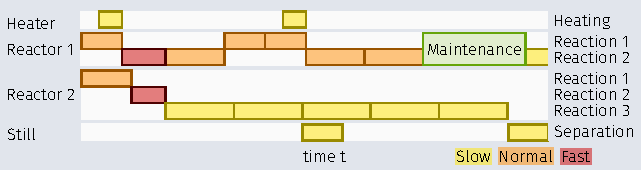
\includegraphics{schedule}
\end{frame}

\begin{frame}[t]{Starting point: Process level MI(N)LP model}
    %\vspace{-10pt}
    \begin{equation*}
    \begin{aligned}
        & \underset{\bm{x},\bm{m}\visible<2->{, {\color{icOrange}\bm{h}}}}{\text{min}}
    && \text{cost}(\bm{x}, \bm{m}\visible<2->{,{\color{icOrange}\bm{h}}})\\
    & \text{s.t.}
    && \text{process model}(\bm{x}, \bm{m}\visible<2->{,{\color{icOrange}\bm{h}}})
    &&& \text{(eg. balance equations)}\\
    &
    && \text{maintenance model}(\bm{x}, \bm{m} \visible<2->{,{\color{icOrange}\bm{h}}})
    &&& \text{(eg. types of maint.)}\\ \visible<2->{&
    && {\color{icOrange}\text{health model}(\bm{x}, \bm{m}, \bm{h})},
    &&& \text{(eq. prognosis model)}}
    \end{aligned}
    \end{equation*}
    where $\bm{x}$ are process variables, $\bm{m}$ are maintenance
    variables\visible<2->{, and {\color{icOrange}$\bm{h}$ are health related variables}.}
    \vspace{5pt}
\only<1-3>{
    \visible<3>{
        \begin{block}{Related Work}
            \small

            Vassiliads and Pistikopoulos (2001); Liu, Yahia and Papageorgiou
            (2014); Xenos, et int., Thornhill (2016); Aguirre and Papageorgiou
            (2018); Biondi, Sand and Harjunkoski (2017); Yildirim, Gebraeel and
            Sun (2017); Ba\c{s}\c{c}iftci, Ahmed, Gebraeel and Yildirim (2018)
            %\citet*{Vassiliadis2001,Liu2014,Xenos2016,Aguirre2018,Biondi2017,Yildirim2017,Basciftci2018}
        \end{block}
    }
}
\only<4->{
    \begin{exampleblock}{Idea}
        Combine process level \textbf{MI(N)LP scheduling \& planning} with more sophisticated (stochastic) \textbf{degradation modelling} and \textbf{robust optimization}.
    \end{exampleblock}
}
\end{frame}

\begin{frame}{What is degradation modelling?}
\only<1>{
    \centering
    \tikzsetnextfilename{deg-sig}
    % Created by tikzDevice version 0.11 on 2018-07-28 20:27:34
% !TEX encoding = UTF-8 Unicode
\begin{tikzpicture}[x=1pt,y=1pt]
\definecolor{fillColor}{RGB}{255,255,255}
\path[use as bounding box,fill=fillColor,fill opacity=0.00] (0,0) rectangle (308.59,216.81);
\begin{scope}
\path[clip] (  0.00,  0.00) rectangle (308.59,216.81);
\definecolor{drawColor}{RGB}{255,255,255}
\definecolor{fillColor}{RGB}{225,229,236}

\path[draw=drawColor,line width= 0.6pt,line join=round,line cap=round,fill=fillColor] (  0.00,  0.00) rectangle (308.59,216.81);
\end{scope}
\begin{scope}
\path[clip] ( 39.22, 30.56) rectangle (303.09,211.31);
\definecolor{fillColor}{gray}{0.98}

\path[fill=fillColor] ( 39.22, 30.56) rectangle (303.09,211.31);
\definecolor{drawColor}{RGB}{210,64,0}

\path[draw=drawColor,line width= 0.6pt,dash pattern=on 4pt off 4pt ,line join=round] ( 51.22,203.09) --
	( 51.46,203.09) --
	( 51.70,203.09) --
	( 51.94,203.09) --
	( 52.18,203.09) --
	( 52.42,203.09) --
	( 52.66,203.09) --
	( 52.90,203.09) --
	( 53.14,203.09) --
	( 53.38,203.09) --
	( 53.62,203.09) --
	( 53.86,203.09) --
	( 54.09,203.09) --
	( 54.33,203.09) --
	( 54.57,203.09) --
	( 54.81,203.09) --
	( 55.05,203.09) --
	( 55.29,203.09) --
	( 55.53,203.09) --
	( 55.77,203.09) --
	( 56.01,203.09) --
	( 56.25,203.09) --
	( 56.49,203.09) --
	( 56.73,203.09) --
	( 56.97,203.09) --
	( 57.21,203.09) --
	( 57.45,203.09) --
	( 57.69,203.09) --
	( 57.93,203.09) --
	( 58.17,203.09) --
	( 58.41,203.09) --
	( 58.65,203.09) --
	( 58.89,203.09) --
	( 59.13,203.09) --
	( 59.37,203.09) --
	( 59.61,203.09) --
	( 59.85,203.09) --
	( 60.09,203.09) --
	( 60.33,203.09) --
	( 60.57,203.09) --
	( 60.81,203.09) --
	( 61.05,203.09) --
	( 61.29,203.09) --
	( 61.53,203.09) --
	( 61.77,203.09) --
	( 62.01,203.09) --
	( 62.25,203.09) --
	( 62.49,203.09) --
	( 62.73,203.09) --
	( 62.97,203.09) --
	( 63.21,203.09) --
	( 63.45,203.09) --
	( 63.69,203.09) --
	( 63.93,203.09) --
	( 64.17,203.09) --
	( 64.41,203.09) --
	( 64.65,203.09) --
	( 64.89,203.09) --
	( 65.13,203.09) --
	( 65.37,203.09) --
	( 65.61,203.09) --
	( 65.85,203.09) --
	( 66.09,203.09) --
	( 66.33,203.09) --
	( 66.57,203.09) --
	( 66.81,203.09) --
	( 67.05,203.09) --
	( 67.29,203.09) --
	( 67.53,203.09) --
	( 67.77,203.09) --
	( 68.01,203.09) --
	( 68.25,203.09) --
	( 68.49,203.09) --
	( 68.73,203.09) --
	( 68.97,203.09) --
	( 69.21,203.09) --
	( 69.45,203.09) --
	( 69.69,203.09) --
	( 69.93,203.09) --
	( 70.17,203.09) --
	( 70.41,203.09) --
	( 70.65,203.09) --
	( 70.89,203.09) --
	( 71.13,203.09) --
	( 71.37,203.09) --
	( 71.61,203.09) --
	( 71.85,203.09) --
	( 72.09,203.09) --
	( 72.33,203.09) --
	( 72.57,203.09) --
	( 72.81,203.09) --
	( 73.05,203.09) --
	( 73.29,203.09) --
	( 73.53,203.09) --
	( 73.77,203.09) --
	( 74.01,203.09) --
	( 74.25,203.09) --
	( 74.48,203.09) --
	( 74.72,203.09) --
	( 74.96,203.09) --
	( 75.20,203.09) --
	( 75.44,203.09) --
	( 75.68,203.09) --
	( 75.92,203.09) --
	( 76.16,203.09) --
	( 76.40,203.09) --
	( 76.64,203.09) --
	( 76.88,203.09) --
	( 77.12,203.09) --
	( 77.36,203.09) --
	( 77.60,203.09) --
	( 77.84,203.09) --
	( 78.08,203.09) --
	( 78.32,203.09) --
	( 78.56,203.09) --
	( 78.80,203.09) --
	( 79.04,203.09) --
	( 79.28,203.09) --
	( 79.52,203.09) --
	( 79.76,203.09) --
	( 80.00,203.09) --
	( 80.24,203.09) --
	( 80.48,203.09) --
	( 80.72,203.09) --
	( 80.96,203.09) --
	( 81.20,203.09) --
	( 81.44,203.09) --
	( 81.68,203.09) --
	( 81.92,203.09) --
	( 82.16,203.09) --
	( 82.40,203.09) --
	( 82.64,203.09) --
	( 82.88,203.09) --
	( 83.12,203.09) --
	( 83.36,203.09) --
	( 83.60,203.09) --
	( 83.84,203.09) --
	( 84.08,203.09) --
	( 84.32,203.09) --
	( 84.56,203.09) --
	( 84.80,203.09) --
	( 85.04,203.09) --
	( 85.28,203.09) --
	( 85.52,203.09) --
	( 85.76,203.09) --
	( 86.00,203.09) --
	( 86.24,203.09) --
	( 86.48,203.09) --
	( 86.72,203.09) --
	( 86.96,203.09) --
	( 87.20,203.09) --
	( 87.44,203.09) --
	( 87.68,203.09) --
	( 87.92,203.09) --
	( 88.16,203.09) --
	( 88.40,203.09) --
	( 88.64,203.09) --
	( 88.88,203.09) --
	( 89.12,203.09) --
	( 89.36,203.09) --
	( 89.60,203.09) --
	( 89.84,203.09) --
	( 90.08,203.09) --
	( 90.32,203.09) --
	( 90.56,203.09) --
	( 90.80,203.09) --
	( 91.04,203.09) --
	( 91.28,203.09) --
	( 91.52,203.09) --
	( 91.76,203.09) --
	( 92.00,203.09) --
	( 92.24,203.09) --
	( 92.48,203.09) --
	( 92.72,203.09) --
	( 92.96,203.09) --
	( 93.20,203.09) --
	( 93.44,203.09) --
	( 93.68,203.09) --
	( 93.92,203.09) --
	( 94.16,203.09) --
	( 94.40,203.09) --
	( 94.64,203.09) --
	( 94.87,203.09) --
	( 95.11,203.09) --
	( 95.35,203.09) --
	( 95.59,203.09) --
	( 95.83,203.09) --
	( 96.07,203.09) --
	( 96.31,203.09) --
	( 96.55,203.09) --
	( 96.79,203.09) --
	( 97.03,203.09) --
	( 97.27,203.09) --
	( 97.51,203.09) --
	( 97.75,203.09) --
	( 97.99,203.09) --
	( 98.23,203.09) --
	( 98.47,203.09) --
	( 98.71,203.09) --
	( 98.95,203.09) --
	( 99.19,203.09) --
	( 99.43,203.09) --
	( 99.67,203.09) --
	( 99.91,203.09) --
	(100.15,203.09) --
	(100.39,203.09) --
	(100.63,203.09) --
	(100.87,203.09) --
	(101.11,203.09) --
	(101.35,203.09) --
	(101.59,203.09) --
	(101.83,203.09) --
	(102.07,203.09) --
	(102.31,203.09) --
	(102.55,203.09) --
	(102.79,203.09) --
	(103.03,203.09) --
	(103.27,203.09) --
	(103.51,203.09) --
	(103.75,203.09) --
	(103.99,203.09) --
	(104.23,203.09) --
	(104.47,203.09) --
	(104.71,203.09) --
	(104.95,203.09) --
	(105.19,203.09) --
	(105.43,203.09) --
	(105.67,203.09) --
	(105.91,203.09) --
	(106.15,203.09) --
	(106.39,203.09) --
	(106.63,203.09) --
	(106.87,203.09) --
	(107.11,203.09) --
	(107.35,203.09) --
	(107.59,203.09) --
	(107.83,203.09) --
	(108.07,203.09) --
	(108.31,203.09) --
	(108.55,203.09) --
	(108.79,203.09) --
	(109.03,203.09) --
	(109.27,203.09) --
	(109.51,203.09) --
	(109.75,203.09) --
	(109.99,203.09) --
	(110.23,203.09) --
	(110.47,203.09) --
	(110.71,203.09) --
	(110.95,203.09) --
	(111.19,203.09) --
	(111.43,203.09) --
	(111.67,203.09) --
	(111.91,203.09) --
	(112.15,203.09) --
	(112.39,203.09) --
	(112.63,203.09) --
	(112.87,203.09) --
	(113.11,203.09) --
	(113.35,203.09) --
	(113.59,203.09) --
	(113.83,203.09) --
	(114.07,203.09) --
	(114.31,203.09) --
	(114.55,203.09) --
	(114.79,203.09) --
	(115.03,203.09) --
	(115.26,203.09) --
	(115.50,203.09) --
	(115.74,203.09) --
	(115.98,203.09) --
	(116.22,203.09) --
	(116.46,203.09) --
	(116.70,203.09) --
	(116.94,203.09) --
	(117.18,203.09) --
	(117.42,203.09) --
	(117.66,203.09) --
	(117.90,203.09) --
	(118.14,203.09) --
	(118.38,203.09) --
	(118.62,203.09) --
	(118.86,203.09) --
	(119.10,203.09) --
	(119.34,203.09) --
	(119.58,203.09) --
	(119.82,203.09) --
	(120.06,203.09) --
	(120.30,203.09) --
	(120.54,203.09) --
	(120.78,203.09) --
	(121.02,203.09) --
	(121.26,203.09) --
	(121.50,203.09) --
	(121.74,203.09) --
	(121.98,203.09) --
	(122.22,203.09) --
	(122.46,203.09) --
	(122.70,203.09) --
	(122.94,203.09) --
	(123.18,203.09) --
	(123.42,203.09) --
	(123.66,203.09) --
	(123.90,203.09) --
	(124.14,203.09) --
	(124.38,203.09) --
	(124.62,203.09) --
	(124.86,203.09) --
	(125.10,203.09) --
	(125.34,203.09) --
	(125.58,203.09) --
	(125.82,203.09) --
	(126.06,203.09) --
	(126.30,203.09) --
	(126.54,203.09) --
	(126.78,203.09) --
	(127.02,203.09) --
	(127.26,203.09) --
	(127.50,203.09) --
	(127.74,203.09) --
	(127.98,203.09) --
	(128.22,203.09) --
	(128.46,203.09) --
	(128.70,203.09) --
	(128.94,203.09) --
	(129.18,203.09) --
	(129.42,203.09) --
	(129.66,203.09) --
	(129.90,203.09) --
	(130.14,203.09) --
	(130.38,203.09) --
	(130.62,203.09) --
	(130.86,203.09) --
	(131.10,203.09) --
	(131.34,203.09) --
	(131.58,203.09) --
	(131.82,203.09) --
	(132.06,203.09) --
	(132.30,203.09) --
	(132.54,203.09) --
	(132.78,203.09) --
	(133.02,203.09) --
	(133.26,203.09) --
	(133.50,203.09) --
	(133.74,203.09) --
	(133.98,203.09) --
	(134.22,203.09) --
	(134.46,203.09) --
	(134.70,203.09) --
	(134.94,203.09) --
	(135.18,203.09) --
	(135.42,203.09) --
	(135.65,203.09) --
	(135.89,203.09) --
	(136.13,203.09) --
	(136.37,203.09) --
	(136.61,203.09) --
	(136.85,203.09) --
	(137.09,203.09) --
	(137.33,203.09) --
	(137.57,203.09) --
	(137.81,203.09) --
	(138.05,203.09) --
	(138.29,203.09) --
	(138.53,203.09) --
	(138.77,203.09) --
	(139.01,203.09) --
	(139.25,203.09) --
	(139.49,203.09) --
	(139.73,203.09) --
	(139.97,203.09) --
	(140.21,203.09) --
	(140.45,203.09) --
	(140.69,203.09) --
	(140.93,203.09) --
	(141.17,203.09) --
	(141.41,203.09) --
	(141.65,203.09) --
	(141.89,203.09) --
	(142.13,203.09) --
	(142.37,203.09) --
	(142.61,203.09) --
	(142.85,203.09) --
	(143.09,203.09) --
	(143.33,203.09) --
	(143.57,203.09) --
	(143.81,203.09) --
	(144.05,203.09) --
	(144.29,203.09) --
	(144.53,203.09) --
	(144.77,203.09) --
	(145.01,203.09) --
	(145.25,203.09) --
	(145.49,203.09) --
	(145.73,203.09) --
	(145.97,203.09) --
	(146.21,203.09) --
	(146.45,203.09) --
	(146.69,203.09) --
	(146.93,203.09) --
	(147.17,203.09) --
	(147.41,203.09) --
	(147.65,203.09) --
	(147.89,203.09) --
	(148.13,203.09) --
	(148.37,203.09) --
	(148.61,203.09) --
	(148.85,203.09) --
	(149.09,203.09) --
	(149.33,203.09) --
	(149.57,203.09) --
	(149.81,203.09) --
	(150.05,203.09) --
	(150.29,203.09) --
	(150.53,203.09) --
	(150.77,203.09) --
	(151.01,203.09) --
	(151.25,203.09) --
	(151.49,203.09) --
	(151.73,203.09) --
	(151.97,203.09) --
	(152.21,203.09) --
	(152.45,203.09) --
	(152.69,203.09) --
	(152.93,203.09) --
	(153.17,203.09) --
	(153.41,203.09) --
	(153.65,203.09) --
	(153.89,203.09) --
	(154.13,203.09) --
	(154.37,203.09) --
	(154.61,203.09) --
	(154.85,203.09) --
	(155.09,203.09) --
	(155.33,203.09) --
	(155.57,203.09) --
	(155.81,203.09) --
	(156.04,203.09) --
	(156.28,203.09) --
	(156.52,203.09) --
	(156.76,203.09) --
	(157.00,203.09) --
	(157.24,203.09) --
	(157.48,203.09) --
	(157.72,203.09) --
	(157.96,203.09) --
	(158.20,203.09) --
	(158.44,203.09) --
	(158.68,203.09) --
	(158.92,203.09) --
	(159.16,203.09) --
	(159.40,203.09) --
	(159.64,203.09) --
	(159.88,203.09) --
	(160.12,203.09) --
	(160.36,203.09) --
	(160.60,203.09) --
	(160.84,203.09) --
	(161.08,203.09) --
	(161.32,203.09) --
	(161.56,203.09) --
	(161.80,203.09) --
	(162.04,203.09) --
	(162.28,203.09) --
	(162.52,203.09) --
	(162.76,203.09) --
	(163.00,203.09) --
	(163.24,203.09) --
	(163.48,203.09) --
	(163.72,203.09) --
	(163.96,203.09) --
	(164.20,203.09) --
	(164.44,203.09) --
	(164.68,203.09) --
	(164.92,203.09) --
	(165.16,203.09) --
	(165.40,203.09) --
	(165.64,203.09) --
	(165.88,203.09) --
	(166.12,203.09) --
	(166.36,203.09) --
	(166.60,203.09) --
	(166.84,203.09) --
	(167.08,203.09) --
	(167.32,203.09) --
	(167.56,203.09) --
	(167.80,203.09) --
	(168.04,203.09) --
	(168.28,203.09) --
	(168.52,203.09) --
	(168.76,203.09) --
	(169.00,203.09) --
	(169.24,203.09) --
	(169.48,203.09) --
	(169.72,203.09) --
	(169.96,203.09) --
	(170.20,203.09) --
	(170.44,203.09) --
	(170.68,203.09) --
	(170.92,203.09) --
	(171.16,203.09) --
	(171.40,203.09) --
	(171.64,203.09) --
	(171.88,203.09) --
	(172.12,203.09) --
	(172.36,203.09) --
	(172.60,203.09) --
	(172.84,203.09) --
	(173.08,203.09) --
	(173.32,203.09) --
	(173.56,203.09) --
	(173.80,203.09) --
	(174.04,203.09) --
	(174.28,203.09) --
	(174.52,203.09) --
	(174.76,203.09) --
	(175.00,203.09) --
	(175.24,203.09) --
	(175.48,203.09) --
	(175.72,203.09) --
	(175.96,203.09) --
	(176.20,203.09) --
	(176.43,203.09) --
	(176.67,203.09) --
	(176.91,203.09) --
	(177.15,203.09) --
	(177.39,203.09) --
	(177.63,203.09) --
	(177.87,203.09) --
	(178.11,203.09) --
	(178.35,203.09) --
	(178.59,203.09) --
	(178.83,203.09) --
	(179.07,203.09) --
	(179.31,203.09) --
	(179.55,203.09) --
	(179.79,203.09) --
	(180.03,203.09) --
	(180.27,203.09) --
	(180.51,203.09) --
	(180.75,203.09) --
	(180.99,203.09) --
	(181.23,203.09) --
	(181.47,203.09) --
	(181.71,203.09) --
	(181.95,203.09) --
	(182.19,203.09) --
	(182.43,203.09) --
	(182.67,203.09) --
	(182.91,203.09) --
	(183.15,203.09) --
	(183.39,203.09) --
	(183.63,203.09) --
	(183.87,203.09) --
	(184.11,203.09) --
	(184.35,203.09) --
	(184.59,203.09) --
	(184.83,203.09) --
	(185.07,203.09) --
	(185.31,203.09) --
	(185.55,203.09) --
	(185.79,203.09) --
	(186.03,203.09) --
	(186.27,203.09) --
	(186.51,203.09) --
	(186.75,203.09) --
	(186.99,203.09) --
	(187.23,203.09) --
	(187.47,203.09) --
	(187.71,203.09) --
	(187.95,203.09) --
	(188.19,203.09) --
	(188.43,203.09) --
	(188.67,203.09) --
	(188.91,203.09) --
	(189.15,203.09) --
	(189.39,203.09) --
	(189.63,203.09) --
	(189.87,203.09) --
	(190.11,203.09) --
	(190.35,203.09) --
	(190.59,203.09) --
	(190.83,203.09) --
	(191.07,203.09) --
	(191.31,203.09) --
	(191.55,203.09) --
	(191.79,203.09) --
	(192.03,203.09) --
	(192.27,203.09) --
	(192.51,203.09) --
	(192.75,203.09) --
	(192.99,203.09) --
	(193.23,203.09) --
	(193.47,203.09) --
	(193.71,203.09) --
	(193.95,203.09) --
	(194.19,203.09) --
	(194.43,203.09) --
	(194.67,203.09) --
	(194.91,203.09) --
	(195.15,203.09) --
	(195.39,203.09) --
	(195.63,203.09) --
	(195.87,203.09) --
	(196.11,203.09) --
	(196.35,203.09) --
	(196.59,203.09) --
	(196.82,203.09) --
	(197.06,203.09) --
	(197.30,203.09) --
	(197.54,203.09) --
	(197.78,203.09) --
	(198.02,203.09) --
	(198.26,203.09) --
	(198.50,203.09) --
	(198.74,203.09) --
	(198.98,203.09) --
	(199.22,203.09) --
	(199.46,203.09) --
	(199.70,203.09) --
	(199.94,203.09) --
	(200.18,203.09) --
	(200.42,203.09) --
	(200.66,203.09) --
	(200.90,203.09) --
	(201.14,203.09) --
	(201.38,203.09) --
	(201.62,203.09) --
	(201.86,203.09) --
	(202.10,203.09) --
	(202.34,203.09) --
	(202.58,203.09) --
	(202.82,203.09) --
	(203.06,203.09) --
	(203.30,203.09) --
	(203.54,203.09) --
	(203.78,203.09) --
	(204.02,203.09) --
	(204.26,203.09) --
	(204.50,203.09) --
	(204.74,203.09) --
	(204.98,203.09) --
	(205.22,203.09) --
	(205.46,203.09) --
	(205.70,203.09) --
	(205.94,203.09) --
	(206.18,203.09) --
	(206.42,203.09) --
	(206.66,203.09) --
	(206.90,203.09) --
	(207.14,203.09) --
	(207.38,203.09) --
	(207.62,203.09) --
	(207.86,203.09) --
	(208.10,203.09) --
	(208.34,203.09) --
	(208.58,203.09) --
	(208.82,203.09) --
	(209.06,203.09) --
	(209.30,203.09) --
	(209.54,203.09) --
	(209.78,203.09) --
	(210.02,203.09) --
	(210.26,203.09) --
	(210.50,203.09) --
	(210.74,203.09) --
	(210.98,203.09) --
	(211.22,203.09) --
	(211.46,203.09) --
	(211.70,203.09) --
	(211.94,203.09) --
	(212.18,203.09) --
	(212.42,203.09) --
	(212.66,203.09) --
	(212.90,203.09) --
	(213.14,203.09) --
	(213.38,203.09) --
	(213.62,203.09) --
	(213.86,203.09) --
	(214.10,203.09) --
	(214.34,203.09) --
	(214.58,203.09) --
	(214.82,203.09) --
	(215.06,203.09) --
	(215.30,203.09) --
	(215.54,203.09) --
	(215.78,203.09) --
	(216.02,203.09) --
	(216.26,203.09) --
	(216.50,203.09) --
	(216.74,203.09) --
	(216.98,203.09) --
	(217.21,203.09) --
	(217.45,203.09) --
	(217.69,203.09) --
	(217.93,203.09) --
	(218.17,203.09) --
	(218.41,203.09) --
	(218.65,203.09) --
	(218.89,203.09) --
	(219.13,203.09) --
	(219.37,203.09) --
	(219.61,203.09) --
	(219.85,203.09) --
	(220.09,203.09) --
	(220.33,203.09) --
	(220.57,203.09) --
	(220.81,203.09) --
	(221.05,203.09) --
	(221.29,203.09) --
	(221.53,203.09) --
	(221.77,203.09) --
	(222.01,203.09) --
	(222.25,203.09) --
	(222.49,203.09) --
	(222.73,203.09) --
	(222.97,203.09) --
	(223.21,203.09) --
	(223.45,203.09) --
	(223.69,203.09) --
	(223.93,203.09) --
	(224.17,203.09) --
	(224.41,203.09) --
	(224.65,203.09) --
	(224.89,203.09) --
	(225.13,203.09) --
	(225.37,203.09) --
	(225.61,203.09) --
	(225.85,203.09) --
	(226.09,203.09) --
	(226.33,203.09) --
	(226.57,203.09) --
	(226.81,203.09) --
	(227.05,203.09) --
	(227.29,203.09) --
	(227.53,203.09) --
	(227.77,203.09) --
	(228.01,203.09) --
	(228.25,203.09) --
	(228.49,203.09) --
	(228.73,203.09) --
	(228.97,203.09) --
	(229.21,203.09) --
	(229.45,203.09) --
	(229.69,203.09) --
	(229.93,203.09) --
	(230.17,203.09) --
	(230.41,203.09) --
	(230.65,203.09) --
	(230.89,203.09) --
	(231.13,203.09) --
	(231.37,203.09) --
	(231.61,203.09) --
	(231.85,203.09) --
	(232.09,203.09) --
	(232.33,203.09) --
	(232.57,203.09) --
	(232.81,203.09) --
	(233.05,203.09) --
	(233.29,203.09) --
	(233.53,203.09) --
	(233.77,203.09) --
	(234.01,203.09) --
	(234.25,203.09) --
	(234.49,203.09) --
	(234.73,203.09) --
	(234.97,203.09) --
	(235.21,203.09) --
	(235.45,203.09) --
	(235.69,203.09) --
	(235.93,203.09) --
	(236.17,203.09) --
	(236.41,203.09) --
	(236.65,203.09) --
	(236.89,203.09) --
	(237.13,203.09) --
	(237.37,203.09) --
	(237.60,203.09) --
	(237.84,203.09) --
	(238.08,203.09) --
	(238.32,203.09) --
	(238.56,203.09) --
	(238.80,203.09) --
	(239.04,203.09) --
	(239.28,203.09) --
	(239.52,203.09) --
	(239.76,203.09) --
	(240.00,203.09) --
	(240.24,203.09) --
	(240.48,203.09) --
	(240.72,203.09) --
	(240.96,203.09) --
	(241.20,203.09) --
	(241.44,203.09) --
	(241.68,203.09) --
	(241.92,203.09) --
	(242.16,203.09) --
	(242.40,203.09) --
	(242.64,203.09) --
	(242.88,203.09) --
	(243.12,203.09) --
	(243.36,203.09) --
	(243.60,203.09) --
	(243.84,203.09) --
	(244.08,203.09) --
	(244.32,203.09) --
	(244.56,203.09) --
	(244.80,203.09) --
	(245.04,203.09) --
	(245.28,203.09) --
	(245.52,203.09) --
	(245.76,203.09) --
	(246.00,203.09) --
	(246.24,203.09) --
	(246.48,203.09) --
	(246.72,203.09) --
	(246.96,203.09) --
	(247.20,203.09) --
	(247.44,203.09) --
	(247.68,203.09) --
	(247.92,203.09) --
	(248.16,203.09) --
	(248.40,203.09) --
	(248.64,203.09) --
	(248.88,203.09) --
	(249.12,203.09) --
	(249.36,203.09) --
	(249.60,203.09) --
	(249.84,203.09) --
	(250.08,203.09) --
	(250.32,203.09) --
	(250.56,203.09) --
	(250.80,203.09) --
	(251.04,203.09) --
	(251.28,203.09) --
	(251.52,203.09) --
	(251.76,203.09) --
	(252.00,203.09) --
	(252.24,203.09) --
	(252.48,203.09) --
	(252.72,203.09) --
	(252.96,203.09) --
	(253.20,203.09) --
	(253.44,203.09) --
	(253.68,203.09) --
	(253.92,203.09) --
	(254.16,203.09) --
	(254.40,203.09) --
	(254.64,203.09) --
	(254.88,203.09) --
	(255.12,203.09) --
	(255.36,203.09) --
	(255.60,203.09) --
	(255.84,203.09) --
	(256.08,203.09) --
	(256.32,203.09) --
	(256.56,203.09) --
	(256.80,203.09) --
	(257.04,203.09) --
	(257.28,203.09) --
	(257.52,203.09) --
	(257.76,203.09) --
	(257.99,203.09) --
	(258.23,203.09) --
	(258.47,203.09) --
	(258.71,203.09) --
	(258.95,203.09) --
	(259.19,203.09) --
	(259.43,203.09) --
	(259.67,203.09) --
	(259.91,203.09) --
	(260.15,203.09) --
	(260.39,203.09) --
	(260.63,203.09) --
	(260.87,203.09) --
	(261.11,203.09) --
	(261.35,203.09) --
	(261.59,203.09) --
	(261.83,203.09) --
	(262.07,203.09) --
	(262.31,203.09) --
	(262.55,203.09) --
	(262.79,203.09) --
	(263.03,203.09) --
	(263.27,203.09) --
	(263.51,203.09) --
	(263.75,203.09) --
	(263.99,203.09) --
	(264.23,203.09) --
	(264.47,203.09) --
	(264.71,203.09) --
	(264.95,203.09) --
	(265.19,203.09) --
	(265.43,203.09) --
	(265.67,203.09) --
	(265.91,203.09) --
	(266.15,203.09) --
	(266.39,203.09) --
	(266.63,203.09) --
	(266.87,203.09) --
	(267.11,203.09) --
	(267.35,203.09) --
	(267.59,203.09) --
	(267.83,203.09) --
	(268.07,203.09) --
	(268.31,203.09) --
	(268.55,203.09) --
	(268.79,203.09) --
	(269.03,203.09) --
	(269.27,203.09) --
	(269.51,203.09) --
	(269.75,203.09) --
	(269.99,203.09) --
	(270.23,203.09) --
	(270.47,203.09) --
	(270.71,203.09) --
	(270.95,203.09) --
	(271.19,203.09) --
	(271.43,203.09) --
	(271.67,203.09) --
	(271.91,203.09) --
	(272.15,203.09) --
	(272.39,203.09) --
	(272.63,203.09) --
	(272.87,203.09) --
	(273.11,203.09) --
	(273.35,203.09) --
	(273.59,203.09) --
	(273.83,203.09) --
	(274.07,203.09) --
	(274.31,203.09) --
	(274.55,203.09) --
	(274.79,203.09) --
	(275.03,203.09) --
	(275.27,203.09) --
	(275.51,203.09) --
	(275.75,203.09) --
	(275.99,203.09) --
	(276.23,203.09) --
	(276.47,203.09) --
	(276.71,203.09) --
	(276.95,203.09) --
	(277.19,203.09) --
	(277.43,203.09) --
	(277.67,203.09) --
	(277.91,203.09) --
	(278.15,203.09) --
	(278.39,203.09) --
	(278.62,203.09) --
	(278.86,203.09) --
	(279.10,203.09) --
	(279.34,203.09) --
	(279.58,203.09) --
	(279.82,203.09) --
	(280.06,203.09) --
	(280.30,203.09) --
	(280.54,203.09) --
	(280.78,203.09) --
	(281.02,203.09) --
	(281.26,203.09) --
	(281.50,203.09) --
	(281.74,203.09) --
	(281.98,203.09) --
	(282.22,203.09) --
	(282.46,203.09) --
	(282.70,203.09) --
	(282.94,203.09) --
	(283.18,203.09) --
	(283.42,203.09) --
	(283.66,203.09) --
	(283.90,203.09) --
	(284.14,203.09) --
	(284.38,203.09) --
	(284.62,203.09) --
	(284.86,203.09) --
	(285.10,203.09) --
	(285.34,203.09) --
	(285.58,203.09) --
	(285.82,203.09) --
	(286.06,203.09) --
	(286.30,203.09) --
	(286.54,203.09) --
	(286.78,203.09) --
	(287.02,203.09) --
	(287.26,203.09) --
	(287.50,203.09) --
	(287.74,203.09) --
	(287.98,203.09) --
	(288.22,203.09) --
	(288.46,203.09) --
	(288.70,203.09) --
	(288.94,203.09) --
	(289.18,203.09) --
	(289.42,203.09) --
	(289.66,203.09) --
	(289.90,203.09) --
	(290.14,203.09) --
	(290.38,203.09) --
	(290.62,203.09) --
	(290.86,203.09) --
	(291.10,203.09);

\node[text=drawColor,anchor=base,inner sep=0pt, outer sep=0pt, scale=  1.10] at ( 81.20,191.08) {$s^{max}$};

\node[text=drawColor,anchor=base,inner sep=0pt, outer sep=0pt, scale=  1.10] at ( 81.20,191.08) {$s^{max}$};

\node[text=drawColor,anchor=base,inner sep=0pt, outer sep=0pt, scale=  1.10] at ( 81.20,191.08) {$s^{max}$};

\node[text=drawColor,anchor=base,inner sep=0pt, outer sep=0pt, scale=  1.10] at ( 81.20,191.08) {$s^{max}$};

\node[text=drawColor,anchor=base,inner sep=0pt, outer sep=0pt, scale=  1.10] at ( 81.20,191.08) {$s^{max}$};

\node[text=drawColor,anchor=base,inner sep=0pt, outer sep=0pt, scale=  1.10] at ( 81.20,191.08) {$s^{max}$};

\node[text=drawColor,anchor=base,inner sep=0pt, outer sep=0pt, scale=  1.10] at ( 81.20,191.08) {$s^{max}$};

\node[text=drawColor,anchor=base,inner sep=0pt, outer sep=0pt, scale=  1.10] at ( 81.20,191.08) {$s^{max}$};

\node[text=drawColor,anchor=base,inner sep=0pt, outer sep=0pt, scale=  1.10] at ( 81.20,191.08) {$s^{max}$};

\node[text=drawColor,anchor=base,inner sep=0pt, outer sep=0pt, scale=  1.10] at ( 81.20,191.08) {$s^{max}$};

\node[text=drawColor,anchor=base,inner sep=0pt, outer sep=0pt, scale=  1.10] at ( 81.20,191.08) {$s^{max}$};

\node[text=drawColor,anchor=base,inner sep=0pt, outer sep=0pt, scale=  1.10] at ( 81.20,191.08) {$s^{max}$};

\node[text=drawColor,anchor=base,inner sep=0pt, outer sep=0pt, scale=  1.10] at ( 81.20,191.08) {$s^{max}$};

\node[text=drawColor,anchor=base,inner sep=0pt, outer sep=0pt, scale=  1.10] at ( 81.20,191.08) {$s^{max}$};

\node[text=drawColor,anchor=base,inner sep=0pt, outer sep=0pt, scale=  1.10] at ( 81.20,191.08) {$s^{max}$};

\node[text=drawColor,anchor=base,inner sep=0pt, outer sep=0pt, scale=  1.10] at ( 81.20,191.08) {$s^{max}$};

\node[text=drawColor,anchor=base,inner sep=0pt, outer sep=0pt, scale=  1.10] at ( 81.20,191.08) {$s^{max}$};

\node[text=drawColor,anchor=base,inner sep=0pt, outer sep=0pt, scale=  1.10] at ( 81.20,191.08) {$s^{max}$};

\node[text=drawColor,anchor=base,inner sep=0pt, outer sep=0pt, scale=  1.10] at ( 81.20,191.08) {$s^{max}$};

\node[text=drawColor,anchor=base,inner sep=0pt, outer sep=0pt, scale=  1.10] at ( 81.20,191.08) {$s^{max}$};

\node[text=drawColor,anchor=base,inner sep=0pt, outer sep=0pt, scale=  1.10] at ( 81.20,191.08) {$s^{max}$};

\node[text=drawColor,anchor=base,inner sep=0pt, outer sep=0pt, scale=  1.10] at ( 81.20,191.08) {$s^{max}$};

\node[text=drawColor,anchor=base,inner sep=0pt, outer sep=0pt, scale=  1.10] at ( 81.20,191.08) {$s^{max}$};

\node[text=drawColor,anchor=base,inner sep=0pt, outer sep=0pt, scale=  1.10] at ( 81.20,191.08) {$s^{max}$};

\node[text=drawColor,anchor=base,inner sep=0pt, outer sep=0pt, scale=  1.10] at ( 81.20,191.08) {$s^{max}$};

\node[text=drawColor,anchor=base,inner sep=0pt, outer sep=0pt, scale=  1.10] at ( 81.20,191.08) {$s^{max}$};

\node[text=drawColor,anchor=base,inner sep=0pt, outer sep=0pt, scale=  1.10] at ( 81.20,191.08) {$s^{max}$};

\node[text=drawColor,anchor=base,inner sep=0pt, outer sep=0pt, scale=  1.10] at ( 81.20,191.08) {$s^{max}$};

\node[text=drawColor,anchor=base,inner sep=0pt, outer sep=0pt, scale=  1.10] at ( 81.20,191.08) {$s^{max}$};

\node[text=drawColor,anchor=base,inner sep=0pt, outer sep=0pt, scale=  1.10] at ( 81.20,191.08) {$s^{max}$};

\node[text=drawColor,anchor=base,inner sep=0pt, outer sep=0pt, scale=  1.10] at ( 81.20,191.08) {$s^{max}$};

\node[text=drawColor,anchor=base,inner sep=0pt, outer sep=0pt, scale=  1.10] at ( 81.20,191.08) {$s^{max}$};

\node[text=drawColor,anchor=base,inner sep=0pt, outer sep=0pt, scale=  1.10] at ( 81.20,191.08) {$s^{max}$};

\node[text=drawColor,anchor=base,inner sep=0pt, outer sep=0pt, scale=  1.10] at ( 81.20,191.08) {$s^{max}$};

\node[text=drawColor,anchor=base,inner sep=0pt, outer sep=0pt, scale=  1.10] at ( 81.20,191.08) {$s^{max}$};

\node[text=drawColor,anchor=base,inner sep=0pt, outer sep=0pt, scale=  1.10] at ( 81.20,191.08) {$s^{max}$};

\node[text=drawColor,anchor=base,inner sep=0pt, outer sep=0pt, scale=  1.10] at ( 81.20,191.08) {$s^{max}$};

\node[text=drawColor,anchor=base,inner sep=0pt, outer sep=0pt, scale=  1.10] at ( 81.20,191.08) {$s^{max}$};

\node[text=drawColor,anchor=base,inner sep=0pt, outer sep=0pt, scale=  1.10] at ( 81.20,191.08) {$s^{max}$};

\node[text=drawColor,anchor=base,inner sep=0pt, outer sep=0pt, scale=  1.10] at ( 81.20,191.08) {$s^{max}$};

\node[text=drawColor,anchor=base,inner sep=0pt, outer sep=0pt, scale=  1.10] at ( 81.20,191.08) {$s^{max}$};

\node[text=drawColor,anchor=base,inner sep=0pt, outer sep=0pt, scale=  1.10] at ( 81.20,191.08) {$s^{max}$};

\node[text=drawColor,anchor=base,inner sep=0pt, outer sep=0pt, scale=  1.10] at ( 81.20,191.08) {$s^{max}$};

\node[text=drawColor,anchor=base,inner sep=0pt, outer sep=0pt, scale=  1.10] at ( 81.20,191.08) {$s^{max}$};

\node[text=drawColor,anchor=base,inner sep=0pt, outer sep=0pt, scale=  1.10] at ( 81.20,191.08) {$s^{max}$};

\node[text=drawColor,anchor=base,inner sep=0pt, outer sep=0pt, scale=  1.10] at ( 81.20,191.08) {$s^{max}$};

\node[text=drawColor,anchor=base,inner sep=0pt, outer sep=0pt, scale=  1.10] at ( 81.20,191.08) {$s^{max}$};

\node[text=drawColor,anchor=base,inner sep=0pt, outer sep=0pt, scale=  1.10] at ( 81.20,191.08) {$s^{max}$};

\node[text=drawColor,anchor=base,inner sep=0pt, outer sep=0pt, scale=  1.10] at ( 81.20,191.08) {$s^{max}$};

\node[text=drawColor,anchor=base,inner sep=0pt, outer sep=0pt, scale=  1.10] at ( 81.20,191.08) {$s^{max}$};

\node[text=drawColor,anchor=base,inner sep=0pt, outer sep=0pt, scale=  1.10] at ( 81.20,191.08) {$s^{max}$};

\node[text=drawColor,anchor=base,inner sep=0pt, outer sep=0pt, scale=  1.10] at ( 81.20,191.08) {$s^{max}$};

\node[text=drawColor,anchor=base,inner sep=0pt, outer sep=0pt, scale=  1.10] at ( 81.20,191.08) {$s^{max}$};

\node[text=drawColor,anchor=base,inner sep=0pt, outer sep=0pt, scale=  1.10] at ( 81.20,191.08) {$s^{max}$};

\node[text=drawColor,anchor=base,inner sep=0pt, outer sep=0pt, scale=  1.10] at ( 81.20,191.08) {$s^{max}$};

\node[text=drawColor,anchor=base,inner sep=0pt, outer sep=0pt, scale=  1.10] at ( 81.20,191.08) {$s^{max}$};

\node[text=drawColor,anchor=base,inner sep=0pt, outer sep=0pt, scale=  1.10] at ( 81.20,191.08) {$s^{max}$};

\node[text=drawColor,anchor=base,inner sep=0pt, outer sep=0pt, scale=  1.10] at ( 81.20,191.08) {$s^{max}$};

\node[text=drawColor,anchor=base,inner sep=0pt, outer sep=0pt, scale=  1.10] at ( 81.20,191.08) {$s^{max}$};

\node[text=drawColor,anchor=base,inner sep=0pt, outer sep=0pt, scale=  1.10] at ( 81.20,191.08) {$s^{max}$};

\node[text=drawColor,anchor=base,inner sep=0pt, outer sep=0pt, scale=  1.10] at ( 81.20,191.08) {$s^{max}$};

\node[text=drawColor,anchor=base,inner sep=0pt, outer sep=0pt, scale=  1.10] at ( 81.20,191.08) {$s^{max}$};

\node[text=drawColor,anchor=base,inner sep=0pt, outer sep=0pt, scale=  1.10] at ( 81.20,191.08) {$s^{max}$};

\node[text=drawColor,anchor=base,inner sep=0pt, outer sep=0pt, scale=  1.10] at ( 81.20,191.08) {$s^{max}$};

\node[text=drawColor,anchor=base,inner sep=0pt, outer sep=0pt, scale=  1.10] at ( 81.20,191.08) {$s^{max}$};

\node[text=drawColor,anchor=base,inner sep=0pt, outer sep=0pt, scale=  1.10] at ( 81.20,191.08) {$s^{max}$};

\node[text=drawColor,anchor=base,inner sep=0pt, outer sep=0pt, scale=  1.10] at ( 81.20,191.08) {$s^{max}$};

\node[text=drawColor,anchor=base,inner sep=0pt, outer sep=0pt, scale=  1.10] at ( 81.20,191.08) {$s^{max}$};

\node[text=drawColor,anchor=base,inner sep=0pt, outer sep=0pt, scale=  1.10] at ( 81.20,191.08) {$s^{max}$};

\node[text=drawColor,anchor=base,inner sep=0pt, outer sep=0pt, scale=  1.10] at ( 81.20,191.08) {$s^{max}$};

\node[text=drawColor,anchor=base,inner sep=0pt, outer sep=0pt, scale=  1.10] at ( 81.20,191.08) {$s^{max}$};

\node[text=drawColor,anchor=base,inner sep=0pt, outer sep=0pt, scale=  1.10] at ( 81.20,191.08) {$s^{max}$};

\node[text=drawColor,anchor=base,inner sep=0pt, outer sep=0pt, scale=  1.10] at ( 81.20,191.08) {$s^{max}$};

\node[text=drawColor,anchor=base,inner sep=0pt, outer sep=0pt, scale=  1.10] at ( 81.20,191.08) {$s^{max}$};

\node[text=drawColor,anchor=base,inner sep=0pt, outer sep=0pt, scale=  1.10] at ( 81.20,191.08) {$s^{max}$};

\node[text=drawColor,anchor=base,inner sep=0pt, outer sep=0pt, scale=  1.10] at ( 81.20,191.08) {$s^{max}$};

\node[text=drawColor,anchor=base,inner sep=0pt, outer sep=0pt, scale=  1.10] at ( 81.20,191.08) {$s^{max}$};

\node[text=drawColor,anchor=base,inner sep=0pt, outer sep=0pt, scale=  1.10] at ( 81.20,191.08) {$s^{max}$};

\node[text=drawColor,anchor=base,inner sep=0pt, outer sep=0pt, scale=  1.10] at ( 81.20,191.08) {$s^{max}$};

\node[text=drawColor,anchor=base,inner sep=0pt, outer sep=0pt, scale=  1.10] at ( 81.20,191.08) {$s^{max}$};

\node[text=drawColor,anchor=base,inner sep=0pt, outer sep=0pt, scale=  1.10] at ( 81.20,191.08) {$s^{max}$};

\node[text=drawColor,anchor=base,inner sep=0pt, outer sep=0pt, scale=  1.10] at ( 81.20,191.08) {$s^{max}$};

\node[text=drawColor,anchor=base,inner sep=0pt, outer sep=0pt, scale=  1.10] at ( 81.20,191.08) {$s^{max}$};

\node[text=drawColor,anchor=base,inner sep=0pt, outer sep=0pt, scale=  1.10] at ( 81.20,191.08) {$s^{max}$};

\node[text=drawColor,anchor=base,inner sep=0pt, outer sep=0pt, scale=  1.10] at ( 81.20,191.08) {$s^{max}$};

\node[text=drawColor,anchor=base,inner sep=0pt, outer sep=0pt, scale=  1.10] at ( 81.20,191.08) {$s^{max}$};

\node[text=drawColor,anchor=base,inner sep=0pt, outer sep=0pt, scale=  1.10] at ( 81.20,191.08) {$s^{max}$};

\node[text=drawColor,anchor=base,inner sep=0pt, outer sep=0pt, scale=  1.10] at ( 81.20,191.08) {$s^{max}$};

\node[text=drawColor,anchor=base,inner sep=0pt, outer sep=0pt, scale=  1.10] at ( 81.20,191.08) {$s^{max}$};

\node[text=drawColor,anchor=base,inner sep=0pt, outer sep=0pt, scale=  1.10] at ( 81.20,191.08) {$s^{max}$};

\node[text=drawColor,anchor=base,inner sep=0pt, outer sep=0pt, scale=  1.10] at ( 81.20,191.08) {$s^{max}$};

\node[text=drawColor,anchor=base,inner sep=0pt, outer sep=0pt, scale=  1.10] at ( 81.20,191.08) {$s^{max}$};

\node[text=drawColor,anchor=base,inner sep=0pt, outer sep=0pt, scale=  1.10] at ( 81.20,191.08) {$s^{max}$};

\node[text=drawColor,anchor=base,inner sep=0pt, outer sep=0pt, scale=  1.10] at ( 81.20,191.08) {$s^{max}$};

\node[text=drawColor,anchor=base,inner sep=0pt, outer sep=0pt, scale=  1.10] at ( 81.20,191.08) {$s^{max}$};

\node[text=drawColor,anchor=base,inner sep=0pt, outer sep=0pt, scale=  1.10] at ( 81.20,191.08) {$s^{max}$};

\node[text=drawColor,anchor=base,inner sep=0pt, outer sep=0pt, scale=  1.10] at ( 81.20,191.08) {$s^{max}$};

\node[text=drawColor,anchor=base,inner sep=0pt, outer sep=0pt, scale=  1.10] at ( 81.20,191.08) {$s^{max}$};

\node[text=drawColor,anchor=base,inner sep=0pt, outer sep=0pt, scale=  1.10] at ( 81.20,191.08) {$s^{max}$};

\node[text=drawColor,anchor=base,inner sep=0pt, outer sep=0pt, scale=  1.10] at ( 81.20,191.08) {$s^{max}$};

\node[text=drawColor,anchor=base,inner sep=0pt, outer sep=0pt, scale=  1.10] at ( 81.20,191.08) {$s^{max}$};

\node[text=drawColor,anchor=base,inner sep=0pt, outer sep=0pt, scale=  1.10] at ( 81.20,191.08) {$s^{max}$};

\node[text=drawColor,anchor=base,inner sep=0pt, outer sep=0pt, scale=  1.10] at ( 81.20,191.08) {$s^{max}$};

\node[text=drawColor,anchor=base,inner sep=0pt, outer sep=0pt, scale=  1.10] at ( 81.20,191.08) {$s^{max}$};

\node[text=drawColor,anchor=base,inner sep=0pt, outer sep=0pt, scale=  1.10] at ( 81.20,191.08) {$s^{max}$};

\node[text=drawColor,anchor=base,inner sep=0pt, outer sep=0pt, scale=  1.10] at ( 81.20,191.08) {$s^{max}$};

\node[text=drawColor,anchor=base,inner sep=0pt, outer sep=0pt, scale=  1.10] at ( 81.20,191.08) {$s^{max}$};

\node[text=drawColor,anchor=base,inner sep=0pt, outer sep=0pt, scale=  1.10] at ( 81.20,191.08) {$s^{max}$};

\node[text=drawColor,anchor=base,inner sep=0pt, outer sep=0pt, scale=  1.10] at ( 81.20,191.08) {$s^{max}$};

\node[text=drawColor,anchor=base,inner sep=0pt, outer sep=0pt, scale=  1.10] at ( 81.20,191.08) {$s^{max}$};

\node[text=drawColor,anchor=base,inner sep=0pt, outer sep=0pt, scale=  1.10] at ( 81.20,191.08) {$s^{max}$};

\node[text=drawColor,anchor=base,inner sep=0pt, outer sep=0pt, scale=  1.10] at ( 81.20,191.08) {$s^{max}$};

\node[text=drawColor,anchor=base,inner sep=0pt, outer sep=0pt, scale=  1.10] at ( 81.20,191.08) {$s^{max}$};

\node[text=drawColor,anchor=base,inner sep=0pt, outer sep=0pt, scale=  1.10] at ( 81.20,191.08) {$s^{max}$};

\node[text=drawColor,anchor=base,inner sep=0pt, outer sep=0pt, scale=  1.10] at ( 81.20,191.08) {$s^{max}$};

\node[text=drawColor,anchor=base,inner sep=0pt, outer sep=0pt, scale=  1.10] at ( 81.20,191.08) {$s^{max}$};

\node[text=drawColor,anchor=base,inner sep=0pt, outer sep=0pt, scale=  1.10] at ( 81.20,191.08) {$s^{max}$};

\node[text=drawColor,anchor=base,inner sep=0pt, outer sep=0pt, scale=  1.10] at ( 81.20,191.08) {$s^{max}$};

\node[text=drawColor,anchor=base,inner sep=0pt, outer sep=0pt, scale=  1.10] at ( 81.20,191.08) {$s^{max}$};

\node[text=drawColor,anchor=base,inner sep=0pt, outer sep=0pt, scale=  1.10] at ( 81.20,191.08) {$s^{max}$};

\node[text=drawColor,anchor=base,inner sep=0pt, outer sep=0pt, scale=  1.10] at ( 81.20,191.08) {$s^{max}$};

\node[text=drawColor,anchor=base,inner sep=0pt, outer sep=0pt, scale=  1.10] at ( 81.20,191.08) {$s^{max}$};

\node[text=drawColor,anchor=base,inner sep=0pt, outer sep=0pt, scale=  1.10] at ( 81.20,191.08) {$s^{max}$};

\node[text=drawColor,anchor=base,inner sep=0pt, outer sep=0pt, scale=  1.10] at ( 81.20,191.08) {$s^{max}$};

\node[text=drawColor,anchor=base,inner sep=0pt, outer sep=0pt, scale=  1.10] at ( 81.20,191.08) {$s^{max}$};

\node[text=drawColor,anchor=base,inner sep=0pt, outer sep=0pt, scale=  1.10] at ( 81.20,191.08) {$s^{max}$};

\node[text=drawColor,anchor=base,inner sep=0pt, outer sep=0pt, scale=  1.10] at ( 81.20,191.08) {$s^{max}$};

\node[text=drawColor,anchor=base,inner sep=0pt, outer sep=0pt, scale=  1.10] at ( 81.20,191.08) {$s^{max}$};

\node[text=drawColor,anchor=base,inner sep=0pt, outer sep=0pt, scale=  1.10] at ( 81.20,191.08) {$s^{max}$};

\node[text=drawColor,anchor=base,inner sep=0pt, outer sep=0pt, scale=  1.10] at ( 81.20,191.08) {$s^{max}$};

\node[text=drawColor,anchor=base,inner sep=0pt, outer sep=0pt, scale=  1.10] at ( 81.20,191.08) {$s^{max}$};

\node[text=drawColor,anchor=base,inner sep=0pt, outer sep=0pt, scale=  1.10] at ( 81.20,191.08) {$s^{max}$};

\node[text=drawColor,anchor=base,inner sep=0pt, outer sep=0pt, scale=  1.10] at ( 81.20,191.08) {$s^{max}$};

\node[text=drawColor,anchor=base,inner sep=0pt, outer sep=0pt, scale=  1.10] at ( 81.20,191.08) {$s^{max}$};

\node[text=drawColor,anchor=base,inner sep=0pt, outer sep=0pt, scale=  1.10] at ( 81.20,191.08) {$s^{max}$};

\node[text=drawColor,anchor=base,inner sep=0pt, outer sep=0pt, scale=  1.10] at ( 81.20,191.08) {$s^{max}$};

\node[text=drawColor,anchor=base,inner sep=0pt, outer sep=0pt, scale=  1.10] at ( 81.20,191.08) {$s^{max}$};

\node[text=drawColor,anchor=base,inner sep=0pt, outer sep=0pt, scale=  1.10] at ( 81.20,191.08) {$s^{max}$};

\node[text=drawColor,anchor=base,inner sep=0pt, outer sep=0pt, scale=  1.10] at ( 81.20,191.08) {$s^{max}$};

\node[text=drawColor,anchor=base,inner sep=0pt, outer sep=0pt, scale=  1.10] at ( 81.20,191.08) {$s^{max}$};

\node[text=drawColor,anchor=base,inner sep=0pt, outer sep=0pt, scale=  1.10] at ( 81.20,191.08) {$s^{max}$};

\node[text=drawColor,anchor=base,inner sep=0pt, outer sep=0pt, scale=  1.10] at ( 81.20,191.08) {$s^{max}$};

\node[text=drawColor,anchor=base,inner sep=0pt, outer sep=0pt, scale=  1.10] at ( 81.20,191.08) {$s^{max}$};

\node[text=drawColor,anchor=base,inner sep=0pt, outer sep=0pt, scale=  1.10] at ( 81.20,191.08) {$s^{max}$};

\node[text=drawColor,anchor=base,inner sep=0pt, outer sep=0pt, scale=  1.10] at ( 81.20,191.08) {$s^{max}$};

\node[text=drawColor,anchor=base,inner sep=0pt, outer sep=0pt, scale=  1.10] at ( 81.20,191.08) {$s^{max}$};

\node[text=drawColor,anchor=base,inner sep=0pt, outer sep=0pt, scale=  1.10] at ( 81.20,191.08) {$s^{max}$};

\node[text=drawColor,anchor=base,inner sep=0pt, outer sep=0pt, scale=  1.10] at ( 81.20,191.08) {$s^{max}$};

\node[text=drawColor,anchor=base,inner sep=0pt, outer sep=0pt, scale=  1.10] at ( 81.20,191.08) {$s^{max}$};

\node[text=drawColor,anchor=base,inner sep=0pt, outer sep=0pt, scale=  1.10] at ( 81.20,191.08) {$s^{max}$};

\node[text=drawColor,anchor=base,inner sep=0pt, outer sep=0pt, scale=  1.10] at ( 81.20,191.08) {$s^{max}$};

\node[text=drawColor,anchor=base,inner sep=0pt, outer sep=0pt, scale=  1.10] at ( 81.20,191.08) {$s^{max}$};

\node[text=drawColor,anchor=base,inner sep=0pt, outer sep=0pt, scale=  1.10] at ( 81.20,191.08) {$s^{max}$};

\node[text=drawColor,anchor=base,inner sep=0pt, outer sep=0pt, scale=  1.10] at ( 81.20,191.08) {$s^{max}$};

\node[text=drawColor,anchor=base,inner sep=0pt, outer sep=0pt, scale=  1.10] at ( 81.20,191.08) {$s^{max}$};

\node[text=drawColor,anchor=base,inner sep=0pt, outer sep=0pt, scale=  1.10] at ( 81.20,191.08) {$s^{max}$};

\node[text=drawColor,anchor=base,inner sep=0pt, outer sep=0pt, scale=  1.10] at ( 81.20,191.08) {$s^{max}$};

\node[text=drawColor,anchor=base,inner sep=0pt, outer sep=0pt, scale=  1.10] at ( 81.20,191.08) {$s^{max}$};

\node[text=drawColor,anchor=base,inner sep=0pt, outer sep=0pt, scale=  1.10] at ( 81.20,191.08) {$s^{max}$};

\node[text=drawColor,anchor=base,inner sep=0pt, outer sep=0pt, scale=  1.10] at ( 81.20,191.08) {$s^{max}$};

\node[text=drawColor,anchor=base,inner sep=0pt, outer sep=0pt, scale=  1.10] at ( 81.20,191.08) {$s^{max}$};

\node[text=drawColor,anchor=base,inner sep=0pt, outer sep=0pt, scale=  1.10] at ( 81.20,191.08) {$s^{max}$};

\node[text=drawColor,anchor=base,inner sep=0pt, outer sep=0pt, scale=  1.10] at ( 81.20,191.08) {$s^{max}$};

\node[text=drawColor,anchor=base,inner sep=0pt, outer sep=0pt, scale=  1.10] at ( 81.20,191.08) {$s^{max}$};

\node[text=drawColor,anchor=base,inner sep=0pt, outer sep=0pt, scale=  1.10] at ( 81.20,191.08) {$s^{max}$};

\node[text=drawColor,anchor=base,inner sep=0pt, outer sep=0pt, scale=  1.10] at ( 81.20,191.08) {$s^{max}$};

\node[text=drawColor,anchor=base,inner sep=0pt, outer sep=0pt, scale=  1.10] at ( 81.20,191.08) {$s^{max}$};

\node[text=drawColor,anchor=base,inner sep=0pt, outer sep=0pt, scale=  1.10] at ( 81.20,191.08) {$s^{max}$};

\node[text=drawColor,anchor=base,inner sep=0pt, outer sep=0pt, scale=  1.10] at ( 81.20,191.08) {$s^{max}$};

\node[text=drawColor,anchor=base,inner sep=0pt, outer sep=0pt, scale=  1.10] at ( 81.20,191.08) {$s^{max}$};

\node[text=drawColor,anchor=base,inner sep=0pt, outer sep=0pt, scale=  1.10] at ( 81.20,191.08) {$s^{max}$};

\node[text=drawColor,anchor=base,inner sep=0pt, outer sep=0pt, scale=  1.10] at ( 81.20,191.08) {$s^{max}$};

\node[text=drawColor,anchor=base,inner sep=0pt, outer sep=0pt, scale=  1.10] at ( 81.20,191.08) {$s^{max}$};

\node[text=drawColor,anchor=base,inner sep=0pt, outer sep=0pt, scale=  1.10] at ( 81.20,191.08) {$s^{max}$};

\node[text=drawColor,anchor=base,inner sep=0pt, outer sep=0pt, scale=  1.10] at ( 81.20,191.08) {$s^{max}$};

\node[text=drawColor,anchor=base,inner sep=0pt, outer sep=0pt, scale=  1.10] at ( 81.20,191.08) {$s^{max}$};

\node[text=drawColor,anchor=base,inner sep=0pt, outer sep=0pt, scale=  1.10] at ( 81.20,191.08) {$s^{max}$};

\node[text=drawColor,anchor=base,inner sep=0pt, outer sep=0pt, scale=  1.10] at ( 81.20,191.08) {$s^{max}$};

\node[text=drawColor,anchor=base,inner sep=0pt, outer sep=0pt, scale=  1.10] at ( 81.20,191.08) {$s^{max}$};

\node[text=drawColor,anchor=base,inner sep=0pt, outer sep=0pt, scale=  1.10] at ( 81.20,191.08) {$s^{max}$};

\node[text=drawColor,anchor=base,inner sep=0pt, outer sep=0pt, scale=  1.10] at ( 81.20,191.08) {$s^{max}$};

\node[text=drawColor,anchor=base,inner sep=0pt, outer sep=0pt, scale=  1.10] at ( 81.20,191.08) {$s^{max}$};

\node[text=drawColor,anchor=base,inner sep=0pt, outer sep=0pt, scale=  1.10] at ( 81.20,191.08) {$s^{max}$};

\node[text=drawColor,anchor=base,inner sep=0pt, outer sep=0pt, scale=  1.10] at ( 81.20,191.08) {$s^{max}$};

\node[text=drawColor,anchor=base,inner sep=0pt, outer sep=0pt, scale=  1.10] at ( 81.20,191.08) {$s^{max}$};

\node[text=drawColor,anchor=base,inner sep=0pt, outer sep=0pt, scale=  1.10] at ( 81.20,191.08) {$s^{max}$};

\node[text=drawColor,anchor=base,inner sep=0pt, outer sep=0pt, scale=  1.10] at ( 81.20,191.08) {$s^{max}$};

\node[text=drawColor,anchor=base,inner sep=0pt, outer sep=0pt, scale=  1.10] at ( 81.20,191.08) {$s^{max}$};

\node[text=drawColor,anchor=base,inner sep=0pt, outer sep=0pt, scale=  1.10] at ( 81.20,191.08) {$s^{max}$};

\node[text=drawColor,anchor=base,inner sep=0pt, outer sep=0pt, scale=  1.10] at ( 81.20,191.08) {$s^{max}$};

\node[text=drawColor,anchor=base,inner sep=0pt, outer sep=0pt, scale=  1.10] at ( 81.20,191.08) {$s^{max}$};

\node[text=drawColor,anchor=base,inner sep=0pt, outer sep=0pt, scale=  1.10] at ( 81.20,191.08) {$s^{max}$};

\node[text=drawColor,anchor=base,inner sep=0pt, outer sep=0pt, scale=  1.10] at ( 81.20,191.08) {$s^{max}$};

\node[text=drawColor,anchor=base,inner sep=0pt, outer sep=0pt, scale=  1.10] at ( 81.20,191.08) {$s^{max}$};

\node[text=drawColor,anchor=base,inner sep=0pt, outer sep=0pt, scale=  1.10] at ( 81.20,191.08) {$s^{max}$};

\node[text=drawColor,anchor=base,inner sep=0pt, outer sep=0pt, scale=  1.10] at ( 81.20,191.08) {$s^{max}$};

\node[text=drawColor,anchor=base,inner sep=0pt, outer sep=0pt, scale=  1.10] at ( 81.20,191.08) {$s^{max}$};

\node[text=drawColor,anchor=base,inner sep=0pt, outer sep=0pt, scale=  1.10] at ( 81.20,191.08) {$s^{max}$};

\node[text=drawColor,anchor=base,inner sep=0pt, outer sep=0pt, scale=  1.10] at ( 81.20,191.08) {$s^{max}$};

\node[text=drawColor,anchor=base,inner sep=0pt, outer sep=0pt, scale=  1.10] at ( 81.20,191.08) {$s^{max}$};

\node[text=drawColor,anchor=base,inner sep=0pt, outer sep=0pt, scale=  1.10] at ( 81.20,191.08) {$s^{max}$};

\node[text=drawColor,anchor=base,inner sep=0pt, outer sep=0pt, scale=  1.10] at ( 81.20,191.08) {$s^{max}$};

\node[text=drawColor,anchor=base,inner sep=0pt, outer sep=0pt, scale=  1.10] at ( 81.20,191.08) {$s^{max}$};

\node[text=drawColor,anchor=base,inner sep=0pt, outer sep=0pt, scale=  1.10] at ( 81.20,191.08) {$s^{max}$};

\node[text=drawColor,anchor=base,inner sep=0pt, outer sep=0pt, scale=  1.10] at ( 81.20,191.08) {$s^{max}$};

\node[text=drawColor,anchor=base,inner sep=0pt, outer sep=0pt, scale=  1.10] at ( 81.20,191.08) {$s^{max}$};

\node[text=drawColor,anchor=base,inner sep=0pt, outer sep=0pt, scale=  1.10] at ( 81.20,191.08) {$s^{max}$};

\node[text=drawColor,anchor=base,inner sep=0pt, outer sep=0pt, scale=  1.10] at ( 81.20,191.08) {$s^{max}$};

\node[text=drawColor,anchor=base,inner sep=0pt, outer sep=0pt, scale=  1.10] at ( 81.20,191.08) {$s^{max}$};

\node[text=drawColor,anchor=base,inner sep=0pt, outer sep=0pt, scale=  1.10] at ( 81.20,191.08) {$s^{max}$};

\node[text=drawColor,anchor=base,inner sep=0pt, outer sep=0pt, scale=  1.10] at ( 81.20,191.08) {$s^{max}$};

\node[text=drawColor,anchor=base,inner sep=0pt, outer sep=0pt, scale=  1.10] at ( 81.20,191.08) {$s^{max}$};

\node[text=drawColor,anchor=base,inner sep=0pt, outer sep=0pt, scale=  1.10] at ( 81.20,191.08) {$s^{max}$};

\node[text=drawColor,anchor=base,inner sep=0pt, outer sep=0pt, scale=  1.10] at ( 81.20,191.08) {$s^{max}$};

\node[text=drawColor,anchor=base,inner sep=0pt, outer sep=0pt, scale=  1.10] at ( 81.20,191.08) {$s^{max}$};

\node[text=drawColor,anchor=base,inner sep=0pt, outer sep=0pt, scale=  1.10] at ( 81.20,191.08) {$s^{max}$};

\node[text=drawColor,anchor=base,inner sep=0pt, outer sep=0pt, scale=  1.10] at ( 81.20,191.08) {$s^{max}$};

\node[text=drawColor,anchor=base,inner sep=0pt, outer sep=0pt, scale=  1.10] at ( 81.20,191.08) {$s^{max}$};

\node[text=drawColor,anchor=base,inner sep=0pt, outer sep=0pt, scale=  1.10] at ( 81.20,191.08) {$s^{max}$};

\node[text=drawColor,anchor=base,inner sep=0pt, outer sep=0pt, scale=  1.10] at ( 81.20,191.08) {$s^{max}$};

\node[text=drawColor,anchor=base,inner sep=0pt, outer sep=0pt, scale=  1.10] at ( 81.20,191.08) {$s^{max}$};

\node[text=drawColor,anchor=base,inner sep=0pt, outer sep=0pt, scale=  1.10] at ( 81.20,191.08) {$s^{max}$};

\node[text=drawColor,anchor=base,inner sep=0pt, outer sep=0pt, scale=  1.10] at ( 81.20,191.08) {$s^{max}$};

\node[text=drawColor,anchor=base,inner sep=0pt, outer sep=0pt, scale=  1.10] at ( 81.20,191.08) {$s^{max}$};

\node[text=drawColor,anchor=base,inner sep=0pt, outer sep=0pt, scale=  1.10] at ( 81.20,191.08) {$s^{max}$};

\node[text=drawColor,anchor=base,inner sep=0pt, outer sep=0pt, scale=  1.10] at ( 81.20,191.08) {$s^{max}$};

\node[text=drawColor,anchor=base,inner sep=0pt, outer sep=0pt, scale=  1.10] at ( 81.20,191.08) {$s^{max}$};

\node[text=drawColor,anchor=base,inner sep=0pt, outer sep=0pt, scale=  1.10] at ( 81.20,191.08) {$s^{max}$};

\node[text=drawColor,anchor=base,inner sep=0pt, outer sep=0pt, scale=  1.10] at ( 81.20,191.08) {$s^{max}$};

\node[text=drawColor,anchor=base,inner sep=0pt, outer sep=0pt, scale=  1.10] at ( 81.20,191.08) {$s^{max}$};

\node[text=drawColor,anchor=base,inner sep=0pt, outer sep=0pt, scale=  1.10] at ( 81.20,191.08) {$s^{max}$};

\node[text=drawColor,anchor=base,inner sep=0pt, outer sep=0pt, scale=  1.10] at ( 81.20,191.08) {$s^{max}$};

\node[text=drawColor,anchor=base,inner sep=0pt, outer sep=0pt, scale=  1.10] at ( 81.20,191.08) {$s^{max}$};

\node[text=drawColor,anchor=base,inner sep=0pt, outer sep=0pt, scale=  1.10] at ( 81.20,191.08) {$s^{max}$};

\node[text=drawColor,anchor=base,inner sep=0pt, outer sep=0pt, scale=  1.10] at ( 81.20,191.08) {$s^{max}$};

\node[text=drawColor,anchor=base,inner sep=0pt, outer sep=0pt, scale=  1.10] at ( 81.20,191.08) {$s^{max}$};

\node[text=drawColor,anchor=base,inner sep=0pt, outer sep=0pt, scale=  1.10] at ( 81.20,191.08) {$s^{max}$};

\node[text=drawColor,anchor=base,inner sep=0pt, outer sep=0pt, scale=  1.10] at ( 81.20,191.08) {$s^{max}$};

\node[text=drawColor,anchor=base,inner sep=0pt, outer sep=0pt, scale=  1.10] at ( 81.20,191.08) {$s^{max}$};

\node[text=drawColor,anchor=base,inner sep=0pt, outer sep=0pt, scale=  1.10] at ( 81.20,191.08) {$s^{max}$};

\node[text=drawColor,anchor=base,inner sep=0pt, outer sep=0pt, scale=  1.10] at ( 81.20,191.08) {$s^{max}$};

\node[text=drawColor,anchor=base,inner sep=0pt, outer sep=0pt, scale=  1.10] at ( 81.20,191.08) {$s^{max}$};

\node[text=drawColor,anchor=base,inner sep=0pt, outer sep=0pt, scale=  1.10] at ( 81.20,191.08) {$s^{max}$};

\node[text=drawColor,anchor=base,inner sep=0pt, outer sep=0pt, scale=  1.10] at ( 81.20,191.08) {$s^{max}$};

\node[text=drawColor,anchor=base,inner sep=0pt, outer sep=0pt, scale=  1.10] at ( 81.20,191.08) {$s^{max}$};

\node[text=drawColor,anchor=base,inner sep=0pt, outer sep=0pt, scale=  1.10] at ( 81.20,191.08) {$s^{max}$};

\node[text=drawColor,anchor=base,inner sep=0pt, outer sep=0pt, scale=  1.10] at ( 81.20,191.08) {$s^{max}$};

\node[text=drawColor,anchor=base,inner sep=0pt, outer sep=0pt, scale=  1.10] at ( 81.20,191.08) {$s^{max}$};

\node[text=drawColor,anchor=base,inner sep=0pt, outer sep=0pt, scale=  1.10] at ( 81.20,191.08) {$s^{max}$};

\node[text=drawColor,anchor=base,inner sep=0pt, outer sep=0pt, scale=  1.10] at ( 81.20,191.08) {$s^{max}$};

\node[text=drawColor,anchor=base,inner sep=0pt, outer sep=0pt, scale=  1.10] at ( 81.20,191.08) {$s^{max}$};

\node[text=drawColor,anchor=base,inner sep=0pt, outer sep=0pt, scale=  1.10] at ( 81.20,191.08) {$s^{max}$};

\node[text=drawColor,anchor=base,inner sep=0pt, outer sep=0pt, scale=  1.10] at ( 81.20,191.08) {$s^{max}$};

\node[text=drawColor,anchor=base,inner sep=0pt, outer sep=0pt, scale=  1.10] at ( 81.20,191.08) {$s^{max}$};

\node[text=drawColor,anchor=base,inner sep=0pt, outer sep=0pt, scale=  1.10] at ( 81.20,191.08) {$s^{max}$};

\node[text=drawColor,anchor=base,inner sep=0pt, outer sep=0pt, scale=  1.10] at ( 81.20,191.08) {$s^{max}$};

\node[text=drawColor,anchor=base,inner sep=0pt, outer sep=0pt, scale=  1.10] at ( 81.20,191.08) {$s^{max}$};

\node[text=drawColor,anchor=base,inner sep=0pt, outer sep=0pt, scale=  1.10] at ( 81.20,191.08) {$s^{max}$};

\node[text=drawColor,anchor=base,inner sep=0pt, outer sep=0pt, scale=  1.10] at ( 81.20,191.08) {$s^{max}$};

\node[text=drawColor,anchor=base,inner sep=0pt, outer sep=0pt, scale=  1.10] at ( 81.20,191.08) {$s^{max}$};

\node[text=drawColor,anchor=base,inner sep=0pt, outer sep=0pt, scale=  1.10] at ( 81.20,191.08) {$s^{max}$};

\node[text=drawColor,anchor=base,inner sep=0pt, outer sep=0pt, scale=  1.10] at ( 81.20,191.08) {$s^{max}$};

\node[text=drawColor,anchor=base,inner sep=0pt, outer sep=0pt, scale=  1.10] at ( 81.20,191.08) {$s^{max}$};

\node[text=drawColor,anchor=base,inner sep=0pt, outer sep=0pt, scale=  1.10] at ( 81.20,191.08) {$s^{max}$};

\node[text=drawColor,anchor=base,inner sep=0pt, outer sep=0pt, scale=  1.10] at ( 81.20,191.08) {$s^{max}$};

\node[text=drawColor,anchor=base,inner sep=0pt, outer sep=0pt, scale=  1.10] at ( 81.20,191.08) {$s^{max}$};

\node[text=drawColor,anchor=base,inner sep=0pt, outer sep=0pt, scale=  1.10] at ( 81.20,191.08) {$s^{max}$};

\node[text=drawColor,anchor=base,inner sep=0pt, outer sep=0pt, scale=  1.10] at ( 81.20,191.08) {$s^{max}$};

\node[text=drawColor,anchor=base,inner sep=0pt, outer sep=0pt, scale=  1.10] at ( 81.20,191.08) {$s^{max}$};

\node[text=drawColor,anchor=base,inner sep=0pt, outer sep=0pt, scale=  1.10] at ( 81.20,191.08) {$s^{max}$};

\node[text=drawColor,anchor=base,inner sep=0pt, outer sep=0pt, scale=  1.10] at ( 81.20,191.08) {$s^{max}$};

\node[text=drawColor,anchor=base,inner sep=0pt, outer sep=0pt, scale=  1.10] at ( 81.20,191.08) {$s^{max}$};

\node[text=drawColor,anchor=base,inner sep=0pt, outer sep=0pt, scale=  1.10] at ( 81.20,191.08) {$s^{max}$};

\node[text=drawColor,anchor=base,inner sep=0pt, outer sep=0pt, scale=  1.10] at ( 81.20,191.08) {$s^{max}$};

\node[text=drawColor,anchor=base,inner sep=0pt, outer sep=0pt, scale=  1.10] at ( 81.20,191.08) {$s^{max}$};

\node[text=drawColor,anchor=base,inner sep=0pt, outer sep=0pt, scale=  1.10] at ( 81.20,191.08) {$s^{max}$};

\node[text=drawColor,anchor=base,inner sep=0pt, outer sep=0pt, scale=  1.10] at ( 81.20,191.08) {$s^{max}$};

\node[text=drawColor,anchor=base,inner sep=0pt, outer sep=0pt, scale=  1.10] at ( 81.20,191.08) {$s^{max}$};

\node[text=drawColor,anchor=base,inner sep=0pt, outer sep=0pt, scale=  1.10] at ( 81.20,191.08) {$s^{max}$};

\node[text=drawColor,anchor=base,inner sep=0pt, outer sep=0pt, scale=  1.10] at ( 81.20,191.08) {$s^{max}$};

\node[text=drawColor,anchor=base,inner sep=0pt, outer sep=0pt, scale=  1.10] at ( 81.20,191.08) {$s^{max}$};

\node[text=drawColor,anchor=base,inner sep=0pt, outer sep=0pt, scale=  1.10] at ( 81.20,191.08) {$s^{max}$};

\node[text=drawColor,anchor=base,inner sep=0pt, outer sep=0pt, scale=  1.10] at ( 81.20,191.08) {$s^{max}$};

\node[text=drawColor,anchor=base,inner sep=0pt, outer sep=0pt, scale=  1.10] at ( 81.20,191.08) {$s^{max}$};

\node[text=drawColor,anchor=base,inner sep=0pt, outer sep=0pt, scale=  1.10] at ( 81.20,191.08) {$s^{max}$};

\node[text=drawColor,anchor=base,inner sep=0pt, outer sep=0pt, scale=  1.10] at ( 81.20,191.08) {$s^{max}$};

\node[text=drawColor,anchor=base,inner sep=0pt, outer sep=0pt, scale=  1.10] at ( 81.20,191.08) {$s^{max}$};

\node[text=drawColor,anchor=base,inner sep=0pt, outer sep=0pt, scale=  1.10] at ( 81.20,191.08) {$s^{max}$};

\node[text=drawColor,anchor=base,inner sep=0pt, outer sep=0pt, scale=  1.10] at ( 81.20,191.08) {$s^{max}$};

\node[text=drawColor,anchor=base,inner sep=0pt, outer sep=0pt, scale=  1.10] at ( 81.20,191.08) {$s^{max}$};

\node[text=drawColor,anchor=base,inner sep=0pt, outer sep=0pt, scale=  1.10] at ( 81.20,191.08) {$s^{max}$};

\node[text=drawColor,anchor=base,inner sep=0pt, outer sep=0pt, scale=  1.10] at ( 81.20,191.08) {$s^{max}$};

\node[text=drawColor,anchor=base,inner sep=0pt, outer sep=0pt, scale=  1.10] at ( 81.20,191.08) {$s^{max}$};

\node[text=drawColor,anchor=base,inner sep=0pt, outer sep=0pt, scale=  1.10] at ( 81.20,191.08) {$s^{max}$};

\node[text=drawColor,anchor=base,inner sep=0pt, outer sep=0pt, scale=  1.10] at ( 81.20,191.08) {$s^{max}$};

\node[text=drawColor,anchor=base,inner sep=0pt, outer sep=0pt, scale=  1.10] at ( 81.20,191.08) {$s^{max}$};

\node[text=drawColor,anchor=base,inner sep=0pt, outer sep=0pt, scale=  1.10] at ( 81.20,191.08) {$s^{max}$};

\node[text=drawColor,anchor=base,inner sep=0pt, outer sep=0pt, scale=  1.10] at ( 81.20,191.08) {$s^{max}$};

\node[text=drawColor,anchor=base,inner sep=0pt, outer sep=0pt, scale=  1.10] at ( 81.20,191.08) {$s^{max}$};

\node[text=drawColor,anchor=base,inner sep=0pt, outer sep=0pt, scale=  1.10] at ( 81.20,191.08) {$s^{max}$};

\node[text=drawColor,anchor=base,inner sep=0pt, outer sep=0pt, scale=  1.10] at ( 81.20,191.08) {$s^{max}$};

\node[text=drawColor,anchor=base,inner sep=0pt, outer sep=0pt, scale=  1.10] at ( 81.20,191.08) {$s^{max}$};

\node[text=drawColor,anchor=base,inner sep=0pt, outer sep=0pt, scale=  1.10] at ( 81.20,191.08) {$s^{max}$};

\node[text=drawColor,anchor=base,inner sep=0pt, outer sep=0pt, scale=  1.10] at ( 81.20,191.08) {$s^{max}$};

\node[text=drawColor,anchor=base,inner sep=0pt, outer sep=0pt, scale=  1.10] at ( 81.20,191.08) {$s^{max}$};

\node[text=drawColor,anchor=base,inner sep=0pt, outer sep=0pt, scale=  1.10] at ( 81.20,191.08) {$s^{max}$};

\node[text=drawColor,anchor=base,inner sep=0pt, outer sep=0pt, scale=  1.10] at ( 81.20,191.08) {$s^{max}$};

\node[text=drawColor,anchor=base,inner sep=0pt, outer sep=0pt, scale=  1.10] at ( 81.20,191.08) {$s^{max}$};

\node[text=drawColor,anchor=base,inner sep=0pt, outer sep=0pt, scale=  1.10] at ( 81.20,191.08) {$s^{max}$};

\node[text=drawColor,anchor=base,inner sep=0pt, outer sep=0pt, scale=  1.10] at ( 81.20,191.08) {$s^{max}$};

\node[text=drawColor,anchor=base,inner sep=0pt, outer sep=0pt, scale=  1.10] at ( 81.20,191.08) {$s^{max}$};

\node[text=drawColor,anchor=base,inner sep=0pt, outer sep=0pt, scale=  1.10] at ( 81.20,191.08) {$s^{max}$};

\node[text=drawColor,anchor=base,inner sep=0pt, outer sep=0pt, scale=  1.10] at ( 81.20,191.08) {$s^{max}$};

\node[text=drawColor,anchor=base,inner sep=0pt, outer sep=0pt, scale=  1.10] at ( 81.20,191.08) {$s^{max}$};

\node[text=drawColor,anchor=base,inner sep=0pt, outer sep=0pt, scale=  1.10] at ( 81.20,191.08) {$s^{max}$};

\node[text=drawColor,anchor=base,inner sep=0pt, outer sep=0pt, scale=  1.10] at ( 81.20,191.08) {$s^{max}$};

\node[text=drawColor,anchor=base,inner sep=0pt, outer sep=0pt, scale=  1.10] at ( 81.20,191.08) {$s^{max}$};

\node[text=drawColor,anchor=base,inner sep=0pt, outer sep=0pt, scale=  1.10] at ( 81.20,191.08) {$s^{max}$};

\node[text=drawColor,anchor=base,inner sep=0pt, outer sep=0pt, scale=  1.10] at ( 81.20,191.08) {$s^{max}$};

\node[text=drawColor,anchor=base,inner sep=0pt, outer sep=0pt, scale=  1.10] at ( 81.20,191.08) {$s^{max}$};

\node[text=drawColor,anchor=base,inner sep=0pt, outer sep=0pt, scale=  1.10] at ( 81.20,191.08) {$s^{max}$};

\node[text=drawColor,anchor=base,inner sep=0pt, outer sep=0pt, scale=  1.10] at ( 81.20,191.08) {$s^{max}$};

\node[text=drawColor,anchor=base,inner sep=0pt, outer sep=0pt, scale=  1.10] at ( 81.20,191.08) {$s^{max}$};

\node[text=drawColor,anchor=base,inner sep=0pt, outer sep=0pt, scale=  1.10] at ( 81.20,191.08) {$s^{max}$};

\node[text=drawColor,anchor=base,inner sep=0pt, outer sep=0pt, scale=  1.10] at ( 81.20,191.08) {$s^{max}$};

\node[text=drawColor,anchor=base,inner sep=0pt, outer sep=0pt, scale=  1.10] at ( 81.20,191.08) {$s^{max}$};

\node[text=drawColor,anchor=base,inner sep=0pt, outer sep=0pt, scale=  1.10] at ( 81.20,191.08) {$s^{max}$};

\node[text=drawColor,anchor=base,inner sep=0pt, outer sep=0pt, scale=  1.10] at ( 81.20,191.08) {$s^{max}$};

\node[text=drawColor,anchor=base,inner sep=0pt, outer sep=0pt, scale=  1.10] at ( 81.20,191.08) {$s^{max}$};

\node[text=drawColor,anchor=base,inner sep=0pt, outer sep=0pt, scale=  1.10] at ( 81.20,191.08) {$s^{max}$};

\node[text=drawColor,anchor=base,inner sep=0pt, outer sep=0pt, scale=  1.10] at ( 81.20,191.08) {$s^{max}$};

\node[text=drawColor,anchor=base,inner sep=0pt, outer sep=0pt, scale=  1.10] at ( 81.20,191.08) {$s^{max}$};

\node[text=drawColor,anchor=base,inner sep=0pt, outer sep=0pt, scale=  1.10] at ( 81.20,191.08) {$s^{max}$};

\node[text=drawColor,anchor=base,inner sep=0pt, outer sep=0pt, scale=  1.10] at ( 81.20,191.08) {$s^{max}$};

\node[text=drawColor,anchor=base,inner sep=0pt, outer sep=0pt, scale=  1.10] at ( 81.20,191.08) {$s^{max}$};

\node[text=drawColor,anchor=base,inner sep=0pt, outer sep=0pt, scale=  1.10] at ( 81.20,191.08) {$s^{max}$};

\node[text=drawColor,anchor=base,inner sep=0pt, outer sep=0pt, scale=  1.10] at ( 81.20,191.08) {$s^{max}$};

\node[text=drawColor,anchor=base,inner sep=0pt, outer sep=0pt, scale=  1.10] at ( 81.20,191.08) {$s^{max}$};

\node[text=drawColor,anchor=base,inner sep=0pt, outer sep=0pt, scale=  1.10] at ( 81.20,191.08) {$s^{max}$};

\node[text=drawColor,anchor=base,inner sep=0pt, outer sep=0pt, scale=  1.10] at ( 81.20,191.08) {$s^{max}$};

\node[text=drawColor,anchor=base,inner sep=0pt, outer sep=0pt, scale=  1.10] at ( 81.20,191.08) {$s^{max}$};

\node[text=drawColor,anchor=base,inner sep=0pt, outer sep=0pt, scale=  1.10] at ( 81.20,191.08) {$s^{max}$};

\node[text=drawColor,anchor=base,inner sep=0pt, outer sep=0pt, scale=  1.10] at ( 81.20,191.08) {$s^{max}$};

\node[text=drawColor,anchor=base,inner sep=0pt, outer sep=0pt, scale=  1.10] at ( 81.20,191.08) {$s^{max}$};

\node[text=drawColor,anchor=base,inner sep=0pt, outer sep=0pt, scale=  1.10] at ( 81.20,191.08) {$s^{max}$};

\node[text=drawColor,anchor=base,inner sep=0pt, outer sep=0pt, scale=  1.10] at ( 81.20,191.08) {$s^{max}$};

\node[text=drawColor,anchor=base,inner sep=0pt, outer sep=0pt, scale=  1.10] at ( 81.20,191.08) {$s^{max}$};

\node[text=drawColor,anchor=base,inner sep=0pt, outer sep=0pt, scale=  1.10] at ( 81.20,191.08) {$s^{max}$};

\node[text=drawColor,anchor=base,inner sep=0pt, outer sep=0pt, scale=  1.10] at ( 81.20,191.08) {$s^{max}$};

\node[text=drawColor,anchor=base,inner sep=0pt, outer sep=0pt, scale=  1.10] at ( 81.20,191.08) {$s^{max}$};

\node[text=drawColor,anchor=base,inner sep=0pt, outer sep=0pt, scale=  1.10] at ( 81.20,191.08) {$s^{max}$};

\node[text=drawColor,anchor=base,inner sep=0pt, outer sep=0pt, scale=  1.10] at ( 81.20,191.08) {$s^{max}$};

\node[text=drawColor,anchor=base,inner sep=0pt, outer sep=0pt, scale=  1.10] at ( 81.20,191.08) {$s^{max}$};

\node[text=drawColor,anchor=base,inner sep=0pt, outer sep=0pt, scale=  1.10] at ( 81.20,191.08) {$s^{max}$};

\node[text=drawColor,anchor=base,inner sep=0pt, outer sep=0pt, scale=  1.10] at ( 81.20,191.08) {$s^{max}$};

\node[text=drawColor,anchor=base,inner sep=0pt, outer sep=0pt, scale=  1.10] at ( 81.20,191.08) {$s^{max}$};

\node[text=drawColor,anchor=base,inner sep=0pt, outer sep=0pt, scale=  1.10] at ( 81.20,191.08) {$s^{max}$};

\node[text=drawColor,anchor=base,inner sep=0pt, outer sep=0pt, scale=  1.10] at ( 81.20,191.08) {$s^{max}$};

\node[text=drawColor,anchor=base,inner sep=0pt, outer sep=0pt, scale=  1.10] at ( 81.20,191.08) {$s^{max}$};

\node[text=drawColor,anchor=base,inner sep=0pt, outer sep=0pt, scale=  1.10] at ( 81.20,191.08) {$s^{max}$};

\node[text=drawColor,anchor=base,inner sep=0pt, outer sep=0pt, scale=  1.10] at ( 81.20,191.08) {$s^{max}$};

\node[text=drawColor,anchor=base,inner sep=0pt, outer sep=0pt, scale=  1.10] at ( 81.20,191.08) {$s^{max}$};

\node[text=drawColor,anchor=base,inner sep=0pt, outer sep=0pt, scale=  1.10] at ( 81.20,191.08) {$s^{max}$};

\node[text=drawColor,anchor=base,inner sep=0pt, outer sep=0pt, scale=  1.10] at ( 81.20,191.08) {$s^{max}$};

\node[text=drawColor,anchor=base,inner sep=0pt, outer sep=0pt, scale=  1.10] at ( 81.20,191.08) {$s^{max}$};

\node[text=drawColor,anchor=base,inner sep=0pt, outer sep=0pt, scale=  1.10] at ( 81.20,191.08) {$s^{max}$};

\node[text=drawColor,anchor=base,inner sep=0pt, outer sep=0pt, scale=  1.10] at ( 81.20,191.08) {$s^{max}$};

\node[text=drawColor,anchor=base,inner sep=0pt, outer sep=0pt, scale=  1.10] at ( 81.20,191.08) {$s^{max}$};

\node[text=drawColor,anchor=base,inner sep=0pt, outer sep=0pt, scale=  1.10] at ( 81.20,191.08) {$s^{max}$};

\node[text=drawColor,anchor=base,inner sep=0pt, outer sep=0pt, scale=  1.10] at ( 81.20,191.08) {$s^{max}$};

\node[text=drawColor,anchor=base,inner sep=0pt, outer sep=0pt, scale=  1.10] at ( 81.20,191.08) {$s^{max}$};

\node[text=drawColor,anchor=base,inner sep=0pt, outer sep=0pt, scale=  1.10] at ( 81.20,191.08) {$s^{max}$};

\node[text=drawColor,anchor=base,inner sep=0pt, outer sep=0pt, scale=  1.10] at ( 81.20,191.08) {$s^{max}$};

\node[text=drawColor,anchor=base,inner sep=0pt, outer sep=0pt, scale=  1.10] at ( 81.20,191.08) {$s^{max}$};

\node[text=drawColor,anchor=base,inner sep=0pt, outer sep=0pt, scale=  1.10] at ( 81.20,191.08) {$s^{max}$};

\node[text=drawColor,anchor=base,inner sep=0pt, outer sep=0pt, scale=  1.10] at ( 81.20,191.08) {$s^{max}$};

\node[text=drawColor,anchor=base,inner sep=0pt, outer sep=0pt, scale=  1.10] at ( 81.20,191.08) {$s^{max}$};

\node[text=drawColor,anchor=base,inner sep=0pt, outer sep=0pt, scale=  1.10] at ( 81.20,191.08) {$s^{max}$};

\node[text=drawColor,anchor=base,inner sep=0pt, outer sep=0pt, scale=  1.10] at ( 81.20,191.08) {$s^{max}$};

\node[text=drawColor,anchor=base,inner sep=0pt, outer sep=0pt, scale=  1.10] at ( 81.20,191.08) {$s^{max}$};

\node[text=drawColor,anchor=base,inner sep=0pt, outer sep=0pt, scale=  1.10] at ( 81.20,191.08) {$s^{max}$};

\node[text=drawColor,anchor=base,inner sep=0pt, outer sep=0pt, scale=  1.10] at ( 81.20,191.08) {$s^{max}$};

\node[text=drawColor,anchor=base,inner sep=0pt, outer sep=0pt, scale=  1.10] at ( 81.20,191.08) {$s^{max}$};

\node[text=drawColor,anchor=base,inner sep=0pt, outer sep=0pt, scale=  1.10] at ( 81.20,191.08) {$s^{max}$};

\node[text=drawColor,anchor=base,inner sep=0pt, outer sep=0pt, scale=  1.10] at ( 81.20,191.08) {$s^{max}$};

\node[text=drawColor,anchor=base,inner sep=0pt, outer sep=0pt, scale=  1.10] at ( 81.20,191.08) {$s^{max}$};

\node[text=drawColor,anchor=base,inner sep=0pt, outer sep=0pt, scale=  1.10] at ( 81.20,191.08) {$s^{max}$};

\node[text=drawColor,anchor=base,inner sep=0pt, outer sep=0pt, scale=  1.10] at ( 81.20,191.08) {$s^{max}$};

\node[text=drawColor,anchor=base,inner sep=0pt, outer sep=0pt, scale=  1.10] at ( 81.20,191.08) {$s^{max}$};

\node[text=drawColor,anchor=base,inner sep=0pt, outer sep=0pt, scale=  1.10] at ( 81.20,191.08) {$s^{max}$};

\node[text=drawColor,anchor=base,inner sep=0pt, outer sep=0pt, scale=  1.10] at ( 81.20,191.08) {$s^{max}$};

\node[text=drawColor,anchor=base,inner sep=0pt, outer sep=0pt, scale=  1.10] at ( 81.20,191.08) {$s^{max}$};

\node[text=drawColor,anchor=base,inner sep=0pt, outer sep=0pt, scale=  1.10] at ( 81.20,191.08) {$s^{max}$};

\node[text=drawColor,anchor=base,inner sep=0pt, outer sep=0pt, scale=  1.10] at ( 81.20,191.08) {$s^{max}$};

\node[text=drawColor,anchor=base,inner sep=0pt, outer sep=0pt, scale=  1.10] at ( 81.20,191.08) {$s^{max}$};

\node[text=drawColor,anchor=base,inner sep=0pt, outer sep=0pt, scale=  1.10] at ( 81.20,191.08) {$s^{max}$};

\node[text=drawColor,anchor=base,inner sep=0pt, outer sep=0pt, scale=  1.10] at ( 81.20,191.08) {$s^{max}$};

\node[text=drawColor,anchor=base,inner sep=0pt, outer sep=0pt, scale=  1.10] at ( 81.20,191.08) {$s^{max}$};

\node[text=drawColor,anchor=base,inner sep=0pt, outer sep=0pt, scale=  1.10] at ( 81.20,191.08) {$s^{max}$};

\node[text=drawColor,anchor=base,inner sep=0pt, outer sep=0pt, scale=  1.10] at ( 81.20,191.08) {$s^{max}$};

\node[text=drawColor,anchor=base,inner sep=0pt, outer sep=0pt, scale=  1.10] at ( 81.20,191.08) {$s^{max}$};

\node[text=drawColor,anchor=base,inner sep=0pt, outer sep=0pt, scale=  1.10] at ( 81.20,191.08) {$s^{max}$};

\node[text=drawColor,anchor=base,inner sep=0pt, outer sep=0pt, scale=  1.10] at ( 81.20,191.08) {$s^{max}$};

\node[text=drawColor,anchor=base,inner sep=0pt, outer sep=0pt, scale=  1.10] at ( 81.20,191.08) {$s^{max}$};

\node[text=drawColor,anchor=base,inner sep=0pt, outer sep=0pt, scale=  1.10] at ( 81.20,191.08) {$s^{max}$};

\node[text=drawColor,anchor=base,inner sep=0pt, outer sep=0pt, scale=  1.10] at ( 81.20,191.08) {$s^{max}$};

\node[text=drawColor,anchor=base,inner sep=0pt, outer sep=0pt, scale=  1.10] at ( 81.20,191.08) {$s^{max}$};

\node[text=drawColor,anchor=base,inner sep=0pt, outer sep=0pt, scale=  1.10] at ( 81.20,191.08) {$s^{max}$};

\node[text=drawColor,anchor=base,inner sep=0pt, outer sep=0pt, scale=  1.10] at ( 81.20,191.08) {$s^{max}$};

\node[text=drawColor,anchor=base,inner sep=0pt, outer sep=0pt, scale=  1.10] at ( 81.20,191.08) {$s^{max}$};

\node[text=drawColor,anchor=base,inner sep=0pt, outer sep=0pt, scale=  1.10] at ( 81.20,191.08) {$s^{max}$};

\node[text=drawColor,anchor=base,inner sep=0pt, outer sep=0pt, scale=  1.10] at ( 81.20,191.08) {$s^{max}$};

\node[text=drawColor,anchor=base,inner sep=0pt, outer sep=0pt, scale=  1.10] at ( 81.20,191.08) {$s^{max}$};

\node[text=drawColor,anchor=base,inner sep=0pt, outer sep=0pt, scale=  1.10] at ( 81.20,191.08) {$s^{max}$};

\node[text=drawColor,anchor=base,inner sep=0pt, outer sep=0pt, scale=  1.10] at ( 81.20,191.08) {$s^{max}$};

\node[text=drawColor,anchor=base,inner sep=0pt, outer sep=0pt, scale=  1.10] at ( 81.20,191.08) {$s^{max}$};

\node[text=drawColor,anchor=base,inner sep=0pt, outer sep=0pt, scale=  1.10] at ( 81.20,191.08) {$s^{max}$};

\node[text=drawColor,anchor=base,inner sep=0pt, outer sep=0pt, scale=  1.10] at ( 81.20,191.08) {$s^{max}$};

\node[text=drawColor,anchor=base,inner sep=0pt, outer sep=0pt, scale=  1.10] at ( 81.20,191.08) {$s^{max}$};

\node[text=drawColor,anchor=base,inner sep=0pt, outer sep=0pt, scale=  1.10] at ( 81.20,191.08) {$s^{max}$};

\node[text=drawColor,anchor=base,inner sep=0pt, outer sep=0pt, scale=  1.10] at ( 81.20,191.08) {$s^{max}$};

\node[text=drawColor,anchor=base,inner sep=0pt, outer sep=0pt, scale=  1.10] at ( 81.20,191.08) {$s^{max}$};

\node[text=drawColor,anchor=base,inner sep=0pt, outer sep=0pt, scale=  1.10] at ( 81.20,191.08) {$s^{max}$};

\node[text=drawColor,anchor=base,inner sep=0pt, outer sep=0pt, scale=  1.10] at ( 81.20,191.08) {$s^{max}$};

\node[text=drawColor,anchor=base,inner sep=0pt, outer sep=0pt, scale=  1.10] at ( 81.20,191.08) {$s^{max}$};

\node[text=drawColor,anchor=base,inner sep=0pt, outer sep=0pt, scale=  1.10] at ( 81.20,191.08) {$s^{max}$};

\node[text=drawColor,anchor=base,inner sep=0pt, outer sep=0pt, scale=  1.10] at ( 81.20,191.08) {$s^{max}$};

\node[text=drawColor,anchor=base,inner sep=0pt, outer sep=0pt, scale=  1.10] at ( 81.20,191.08) {$s^{max}$};

\node[text=drawColor,anchor=base,inner sep=0pt, outer sep=0pt, scale=  1.10] at ( 81.20,191.08) {$s^{max}$};

\node[text=drawColor,anchor=base,inner sep=0pt, outer sep=0pt, scale=  1.10] at ( 81.20,191.08) {$s^{max}$};

\node[text=drawColor,anchor=base,inner sep=0pt, outer sep=0pt, scale=  1.10] at ( 81.20,191.08) {$s^{max}$};

\node[text=drawColor,anchor=base,inner sep=0pt, outer sep=0pt, scale=  1.10] at ( 81.20,191.08) {$s^{max}$};

\node[text=drawColor,anchor=base,inner sep=0pt, outer sep=0pt, scale=  1.10] at ( 81.20,191.08) {$s^{max}$};

\node[text=drawColor,anchor=base,inner sep=0pt, outer sep=0pt, scale=  1.10] at ( 81.20,191.08) {$s^{max}$};

\node[text=drawColor,anchor=base,inner sep=0pt, outer sep=0pt, scale=  1.10] at ( 81.20,191.08) {$s^{max}$};

\node[text=drawColor,anchor=base,inner sep=0pt, outer sep=0pt, scale=  1.10] at ( 81.20,191.08) {$s^{max}$};

\node[text=drawColor,anchor=base,inner sep=0pt, outer sep=0pt, scale=  1.10] at ( 81.20,191.08) {$s^{max}$};

\node[text=drawColor,anchor=base,inner sep=0pt, outer sep=0pt, scale=  1.10] at ( 81.20,191.08) {$s^{max}$};

\node[text=drawColor,anchor=base,inner sep=0pt, outer sep=0pt, scale=  1.10] at ( 81.20,191.08) {$s^{max}$};

\node[text=drawColor,anchor=base,inner sep=0pt, outer sep=0pt, scale=  1.10] at ( 81.20,191.08) {$s^{max}$};

\node[text=drawColor,anchor=base,inner sep=0pt, outer sep=0pt, scale=  1.10] at ( 81.20,191.08) {$s^{max}$};

\node[text=drawColor,anchor=base,inner sep=0pt, outer sep=0pt, scale=  1.10] at ( 81.20,191.08) {$s^{max}$};

\node[text=drawColor,anchor=base,inner sep=0pt, outer sep=0pt, scale=  1.10] at ( 81.20,191.08) {$s^{max}$};

\node[text=drawColor,anchor=base,inner sep=0pt, outer sep=0pt, scale=  1.10] at ( 81.20,191.08) {$s^{max}$};

\node[text=drawColor,anchor=base,inner sep=0pt, outer sep=0pt, scale=  1.10] at ( 81.20,191.08) {$s^{max}$};

\node[text=drawColor,anchor=base,inner sep=0pt, outer sep=0pt, scale=  1.10] at ( 81.20,191.08) {$s^{max}$};

\node[text=drawColor,anchor=base,inner sep=0pt, outer sep=0pt, scale=  1.10] at ( 81.20,191.08) {$s^{max}$};

\node[text=drawColor,anchor=base,inner sep=0pt, outer sep=0pt, scale=  1.10] at ( 81.20,191.08) {$s^{max}$};

\node[text=drawColor,anchor=base,inner sep=0pt, outer sep=0pt, scale=  1.10] at ( 81.20,191.08) {$s^{max}$};

\node[text=drawColor,anchor=base,inner sep=0pt, outer sep=0pt, scale=  1.10] at ( 81.20,191.08) {$s^{max}$};

\node[text=drawColor,anchor=base,inner sep=0pt, outer sep=0pt, scale=  1.10] at ( 81.20,191.08) {$s^{max}$};

\node[text=drawColor,anchor=base,inner sep=0pt, outer sep=0pt, scale=  1.10] at ( 81.20,191.08) {$s^{max}$};

\node[text=drawColor,anchor=base,inner sep=0pt, outer sep=0pt, scale=  1.10] at ( 81.20,191.08) {$s^{max}$};

\node[text=drawColor,anchor=base,inner sep=0pt, outer sep=0pt, scale=  1.10] at ( 81.20,191.08) {$s^{max}$};

\node[text=drawColor,anchor=base,inner sep=0pt, outer sep=0pt, scale=  1.10] at ( 81.20,191.08) {$s^{max}$};

\node[text=drawColor,anchor=base,inner sep=0pt, outer sep=0pt, scale=  1.10] at ( 81.20,191.08) {$s^{max}$};

\node[text=drawColor,anchor=base,inner sep=0pt, outer sep=0pt, scale=  1.10] at ( 81.20,191.08) {$s^{max}$};

\node[text=drawColor,anchor=base,inner sep=0pt, outer sep=0pt, scale=  1.10] at ( 81.20,191.08) {$s^{max}$};

\node[text=drawColor,anchor=base,inner sep=0pt, outer sep=0pt, scale=  1.10] at ( 81.20,191.08) {$s^{max}$};

\node[text=drawColor,anchor=base,inner sep=0pt, outer sep=0pt, scale=  1.10] at ( 81.20,191.08) {$s^{max}$};

\node[text=drawColor,anchor=base,inner sep=0pt, outer sep=0pt, scale=  1.10] at ( 81.20,191.08) {$s^{max}$};

\node[text=drawColor,anchor=base,inner sep=0pt, outer sep=0pt, scale=  1.10] at ( 81.20,191.08) {$s^{max}$};

\node[text=drawColor,anchor=base,inner sep=0pt, outer sep=0pt, scale=  1.10] at ( 81.20,191.08) {$s^{max}$};

\node[text=drawColor,anchor=base,inner sep=0pt, outer sep=0pt, scale=  1.10] at ( 81.20,191.08) {$s^{max}$};

\node[text=drawColor,anchor=base,inner sep=0pt, outer sep=0pt, scale=  1.10] at ( 81.20,191.08) {$s^{max}$};

\node[text=drawColor,anchor=base,inner sep=0pt, outer sep=0pt, scale=  1.10] at ( 81.20,191.08) {$s^{max}$};

\node[text=drawColor,anchor=base,inner sep=0pt, outer sep=0pt, scale=  1.10] at ( 81.20,191.08) {$s^{max}$};

\node[text=drawColor,anchor=base,inner sep=0pt, outer sep=0pt, scale=  1.10] at ( 81.20,191.08) {$s^{max}$};

\node[text=drawColor,anchor=base,inner sep=0pt, outer sep=0pt, scale=  1.10] at ( 81.20,191.08) {$s^{max}$};

\node[text=drawColor,anchor=base,inner sep=0pt, outer sep=0pt, scale=  1.10] at ( 81.20,191.08) {$s^{max}$};

\node[text=drawColor,anchor=base,inner sep=0pt, outer sep=0pt, scale=  1.10] at ( 81.20,191.08) {$s^{max}$};

\node[text=drawColor,anchor=base,inner sep=0pt, outer sep=0pt, scale=  1.10] at ( 81.20,191.08) {$s^{max}$};

\node[text=drawColor,anchor=base,inner sep=0pt, outer sep=0pt, scale=  1.10] at ( 81.20,191.08) {$s^{max}$};

\node[text=drawColor,anchor=base,inner sep=0pt, outer sep=0pt, scale=  1.10] at ( 81.20,191.08) {$s^{max}$};

\node[text=drawColor,anchor=base,inner sep=0pt, outer sep=0pt, scale=  1.10] at ( 81.20,191.08) {$s^{max}$};

\node[text=drawColor,anchor=base,inner sep=0pt, outer sep=0pt, scale=  1.10] at ( 81.20,191.08) {$s^{max}$};

\node[text=drawColor,anchor=base,inner sep=0pt, outer sep=0pt, scale=  1.10] at ( 81.20,191.08) {$s^{max}$};

\node[text=drawColor,anchor=base,inner sep=0pt, outer sep=0pt, scale=  1.10] at ( 81.20,191.08) {$s^{max}$};

\node[text=drawColor,anchor=base,inner sep=0pt, outer sep=0pt, scale=  1.10] at ( 81.20,191.08) {$s^{max}$};

\node[text=drawColor,anchor=base,inner sep=0pt, outer sep=0pt, scale=  1.10] at ( 81.20,191.08) {$s^{max}$};

\node[text=drawColor,anchor=base,inner sep=0pt, outer sep=0pt, scale=  1.10] at ( 81.20,191.08) {$s^{max}$};

\node[text=drawColor,anchor=base,inner sep=0pt, outer sep=0pt, scale=  1.10] at ( 81.20,191.08) {$s^{max}$};

\node[text=drawColor,anchor=base,inner sep=0pt, outer sep=0pt, scale=  1.10] at ( 81.20,191.08) {$s^{max}$};

\node[text=drawColor,anchor=base,inner sep=0pt, outer sep=0pt, scale=  1.10] at ( 81.20,191.08) {$s^{max}$};

\node[text=drawColor,anchor=base,inner sep=0pt, outer sep=0pt, scale=  1.10] at ( 81.20,191.08) {$s^{max}$};

\node[text=drawColor,anchor=base,inner sep=0pt, outer sep=0pt, scale=  1.10] at ( 81.20,191.08) {$s^{max}$};

\node[text=drawColor,anchor=base,inner sep=0pt, outer sep=0pt, scale=  1.10] at ( 81.20,191.08) {$s^{max}$};

\node[text=drawColor,anchor=base,inner sep=0pt, outer sep=0pt, scale=  1.10] at ( 81.20,191.08) {$s^{max}$};

\node[text=drawColor,anchor=base,inner sep=0pt, outer sep=0pt, scale=  1.10] at ( 81.20,191.08) {$s^{max}$};

\node[text=drawColor,anchor=base,inner sep=0pt, outer sep=0pt, scale=  1.10] at ( 81.20,191.08) {$s^{max}$};

\node[text=drawColor,anchor=base,inner sep=0pt, outer sep=0pt, scale=  1.10] at ( 81.20,191.08) {$s^{max}$};

\node[text=drawColor,anchor=base,inner sep=0pt, outer sep=0pt, scale=  1.10] at ( 81.20,191.08) {$s^{max}$};

\node[text=drawColor,anchor=base,inner sep=0pt, outer sep=0pt, scale=  1.10] at ( 81.20,191.08) {$s^{max}$};

\node[text=drawColor,anchor=base,inner sep=0pt, outer sep=0pt, scale=  1.10] at ( 81.20,191.08) {$s^{max}$};

\node[text=drawColor,anchor=base,inner sep=0pt, outer sep=0pt, scale=  1.10] at ( 81.20,191.08) {$s^{max}$};

\node[text=drawColor,anchor=base,inner sep=0pt, outer sep=0pt, scale=  1.10] at ( 81.20,191.08) {$s^{max}$};

\node[text=drawColor,anchor=base,inner sep=0pt, outer sep=0pt, scale=  1.10] at ( 81.20,191.08) {$s^{max}$};

\node[text=drawColor,anchor=base,inner sep=0pt, outer sep=0pt, scale=  1.10] at ( 81.20,191.08) {$s^{max}$};

\node[text=drawColor,anchor=base,inner sep=0pt, outer sep=0pt, scale=  1.10] at ( 81.20,191.08) {$s^{max}$};

\node[text=drawColor,anchor=base,inner sep=0pt, outer sep=0pt, scale=  1.10] at ( 81.20,191.08) {$s^{max}$};

\node[text=drawColor,anchor=base,inner sep=0pt, outer sep=0pt, scale=  1.10] at ( 81.20,191.08) {$s^{max}$};

\node[text=drawColor,anchor=base,inner sep=0pt, outer sep=0pt, scale=  1.10] at ( 81.20,191.08) {$s^{max}$};

\node[text=drawColor,anchor=base,inner sep=0pt, outer sep=0pt, scale=  1.10] at ( 81.20,191.08) {$s^{max}$};

\node[text=drawColor,anchor=base,inner sep=0pt, outer sep=0pt, scale=  1.10] at ( 81.20,191.08) {$s^{max}$};

\node[text=drawColor,anchor=base,inner sep=0pt, outer sep=0pt, scale=  1.10] at ( 81.20,191.08) {$s^{max}$};

\node[text=drawColor,anchor=base,inner sep=0pt, outer sep=0pt, scale=  1.10] at ( 81.20,191.08) {$s^{max}$};

\node[text=drawColor,anchor=base,inner sep=0pt, outer sep=0pt, scale=  1.10] at ( 81.20,191.08) {$s^{max}$};

\node[text=drawColor,anchor=base,inner sep=0pt, outer sep=0pt, scale=  1.10] at ( 81.20,191.08) {$s^{max}$};

\node[text=drawColor,anchor=base,inner sep=0pt, outer sep=0pt, scale=  1.10] at ( 81.20,191.08) {$s^{max}$};

\node[text=drawColor,anchor=base,inner sep=0pt, outer sep=0pt, scale=  1.10] at ( 81.20,191.08) {$s^{max}$};

\node[text=drawColor,anchor=base,inner sep=0pt, outer sep=0pt, scale=  1.10] at ( 81.20,191.08) {$s^{max}$};

\node[text=drawColor,anchor=base,inner sep=0pt, outer sep=0pt, scale=  1.10] at ( 81.20,191.08) {$s^{max}$};

\node[text=drawColor,anchor=base,inner sep=0pt, outer sep=0pt, scale=  1.10] at ( 81.20,191.08) {$s^{max}$};

\node[text=drawColor,anchor=base,inner sep=0pt, outer sep=0pt, scale=  1.10] at ( 81.20,191.08) {$s^{max}$};

\node[text=drawColor,anchor=base,inner sep=0pt, outer sep=0pt, scale=  1.10] at ( 81.20,191.08) {$s^{max}$};

\node[text=drawColor,anchor=base,inner sep=0pt, outer sep=0pt, scale=  1.10] at ( 81.20,191.08) {$s^{max}$};

\node[text=drawColor,anchor=base,inner sep=0pt, outer sep=0pt, scale=  1.10] at ( 81.20,191.08) {$s^{max}$};

\node[text=drawColor,anchor=base,inner sep=0pt, outer sep=0pt, scale=  1.10] at ( 81.20,191.08) {$s^{max}$};

\node[text=drawColor,anchor=base,inner sep=0pt, outer sep=0pt, scale=  1.10] at ( 81.20,191.08) {$s^{max}$};

\node[text=drawColor,anchor=base,inner sep=0pt, outer sep=0pt, scale=  1.10] at ( 81.20,191.08) {$s^{max}$};

\node[text=drawColor,anchor=base,inner sep=0pt, outer sep=0pt, scale=  1.10] at ( 81.20,191.08) {$s^{max}$};

\node[text=drawColor,anchor=base,inner sep=0pt, outer sep=0pt, scale=  1.10] at ( 81.20,191.08) {$s^{max}$};

\node[text=drawColor,anchor=base,inner sep=0pt, outer sep=0pt, scale=  1.10] at ( 81.20,191.08) {$s^{max}$};

\node[text=drawColor,anchor=base,inner sep=0pt, outer sep=0pt, scale=  1.10] at ( 81.20,191.08) {$s^{max}$};

\node[text=drawColor,anchor=base,inner sep=0pt, outer sep=0pt, scale=  1.10] at ( 81.20,191.08) {$s^{max}$};

\node[text=drawColor,anchor=base,inner sep=0pt, outer sep=0pt, scale=  1.10] at ( 81.20,191.08) {$s^{max}$};

\node[text=drawColor,anchor=base,inner sep=0pt, outer sep=0pt, scale=  1.10] at ( 81.20,191.08) {$s^{max}$};

\node[text=drawColor,anchor=base,inner sep=0pt, outer sep=0pt, scale=  1.10] at ( 81.20,191.08) {$s^{max}$};

\node[text=drawColor,anchor=base,inner sep=0pt, outer sep=0pt, scale=  1.10] at ( 81.20,191.08) {$s^{max}$};

\node[text=drawColor,anchor=base,inner sep=0pt, outer sep=0pt, scale=  1.10] at ( 81.20,191.08) {$s^{max}$};

\node[text=drawColor,anchor=base,inner sep=0pt, outer sep=0pt, scale=  1.10] at ( 81.20,191.08) {$s^{max}$};

\node[text=drawColor,anchor=base,inner sep=0pt, outer sep=0pt, scale=  1.10] at ( 81.20,191.08) {$s^{max}$};

\node[text=drawColor,anchor=base,inner sep=0pt, outer sep=0pt, scale=  1.10] at ( 81.20,191.08) {$s^{max}$};

\node[text=drawColor,anchor=base,inner sep=0pt, outer sep=0pt, scale=  1.10] at ( 81.20,191.08) {$s^{max}$};

\node[text=drawColor,anchor=base,inner sep=0pt, outer sep=0pt, scale=  1.10] at ( 81.20,191.08) {$s^{max}$};

\node[text=drawColor,anchor=base,inner sep=0pt, outer sep=0pt, scale=  1.10] at ( 81.20,191.08) {$s^{max}$};

\node[text=drawColor,anchor=base,inner sep=0pt, outer sep=0pt, scale=  1.10] at ( 81.20,191.08) {$s^{max}$};

\node[text=drawColor,anchor=base,inner sep=0pt, outer sep=0pt, scale=  1.10] at ( 81.20,191.08) {$s^{max}$};

\node[text=drawColor,anchor=base,inner sep=0pt, outer sep=0pt, scale=  1.10] at ( 81.20,191.08) {$s^{max}$};

\node[text=drawColor,anchor=base,inner sep=0pt, outer sep=0pt, scale=  1.10] at ( 81.20,191.08) {$s^{max}$};

\node[text=drawColor,anchor=base,inner sep=0pt, outer sep=0pt, scale=  1.10] at ( 81.20,191.08) {$s^{max}$};

\node[text=drawColor,anchor=base,inner sep=0pt, outer sep=0pt, scale=  1.10] at ( 81.20,191.08) {$s^{max}$};

\node[text=drawColor,anchor=base,inner sep=0pt, outer sep=0pt, scale=  1.10] at ( 81.20,191.08) {$s^{max}$};

\node[text=drawColor,anchor=base,inner sep=0pt, outer sep=0pt, scale=  1.10] at ( 81.20,191.08) {$s^{max}$};

\node[text=drawColor,anchor=base,inner sep=0pt, outer sep=0pt, scale=  1.10] at ( 81.20,191.08) {$s^{max}$};

\node[text=drawColor,anchor=base,inner sep=0pt, outer sep=0pt, scale=  1.10] at ( 81.20,191.08) {$s^{max}$};

\node[text=drawColor,anchor=base,inner sep=0pt, outer sep=0pt, scale=  1.10] at ( 81.20,191.08) {$s^{max}$};

\node[text=drawColor,anchor=base,inner sep=0pt, outer sep=0pt, scale=  1.10] at ( 81.20,191.08) {$s^{max}$};

\node[text=drawColor,anchor=base,inner sep=0pt, outer sep=0pt, scale=  1.10] at ( 81.20,191.08) {$s^{max}$};

\node[text=drawColor,anchor=base,inner sep=0pt, outer sep=0pt, scale=  1.10] at ( 81.20,191.08) {$s^{max}$};

\node[text=drawColor,anchor=base,inner sep=0pt, outer sep=0pt, scale=  1.10] at ( 81.20,191.08) {$s^{max}$};

\node[text=drawColor,anchor=base,inner sep=0pt, outer sep=0pt, scale=  1.10] at ( 81.20,191.08) {$s^{max}$};

\node[text=drawColor,anchor=base,inner sep=0pt, outer sep=0pt, scale=  1.10] at ( 81.20,191.08) {$s^{max}$};

\node[text=drawColor,anchor=base,inner sep=0pt, outer sep=0pt, scale=  1.10] at ( 81.20,191.08) {$s^{max}$};

\node[text=drawColor,anchor=base,inner sep=0pt, outer sep=0pt, scale=  1.10] at ( 81.20,191.08) {$s^{max}$};

\node[text=drawColor,anchor=base,inner sep=0pt, outer sep=0pt, scale=  1.10] at ( 81.20,191.08) {$s^{max}$};

\node[text=drawColor,anchor=base,inner sep=0pt, outer sep=0pt, scale=  1.10] at ( 81.20,191.08) {$s^{max}$};

\node[text=drawColor,anchor=base,inner sep=0pt, outer sep=0pt, scale=  1.10] at ( 81.20,191.08) {$s^{max}$};

\node[text=drawColor,anchor=base,inner sep=0pt, outer sep=0pt, scale=  1.10] at ( 81.20,191.08) {$s^{max}$};

\node[text=drawColor,anchor=base,inner sep=0pt, outer sep=0pt, scale=  1.10] at ( 81.20,191.08) {$s^{max}$};

\node[text=drawColor,anchor=base,inner sep=0pt, outer sep=0pt, scale=  1.10] at ( 81.20,191.08) {$s^{max}$};

\node[text=drawColor,anchor=base,inner sep=0pt, outer sep=0pt, scale=  1.10] at ( 81.20,191.08) {$s^{max}$};

\node[text=drawColor,anchor=base,inner sep=0pt, outer sep=0pt, scale=  1.10] at ( 81.20,191.08) {$s^{max}$};

\node[text=drawColor,anchor=base,inner sep=0pt, outer sep=0pt, scale=  1.10] at ( 81.20,191.08) {$s^{max}$};

\node[text=drawColor,anchor=base,inner sep=0pt, outer sep=0pt, scale=  1.10] at ( 81.20,191.08) {$s^{max}$};

\node[text=drawColor,anchor=base,inner sep=0pt, outer sep=0pt, scale=  1.10] at ( 81.20,191.08) {$s^{max}$};

\node[text=drawColor,anchor=base,inner sep=0pt, outer sep=0pt, scale=  1.10] at ( 81.20,191.08) {$s^{max}$};

\node[text=drawColor,anchor=base,inner sep=0pt, outer sep=0pt, scale=  1.10] at ( 81.20,191.08) {$s^{max}$};

\node[text=drawColor,anchor=base,inner sep=0pt, outer sep=0pt, scale=  1.10] at ( 81.20,191.08) {$s^{max}$};

\node[text=drawColor,anchor=base,inner sep=0pt, outer sep=0pt, scale=  1.10] at ( 81.20,191.08) {$s^{max}$};

\node[text=drawColor,anchor=base,inner sep=0pt, outer sep=0pt, scale=  1.10] at ( 81.20,191.08) {$s^{max}$};

\node[text=drawColor,anchor=base,inner sep=0pt, outer sep=0pt, scale=  1.10] at ( 81.20,191.08) {$s^{max}$};

\node[text=drawColor,anchor=base,inner sep=0pt, outer sep=0pt, scale=  1.10] at ( 81.20,191.08) {$s^{max}$};

\node[text=drawColor,anchor=base,inner sep=0pt, outer sep=0pt, scale=  1.10] at ( 81.20,191.08) {$s^{max}$};

\node[text=drawColor,anchor=base,inner sep=0pt, outer sep=0pt, scale=  1.10] at ( 81.20,191.08) {$s^{max}$};

\node[text=drawColor,anchor=base,inner sep=0pt, outer sep=0pt, scale=  1.10] at ( 81.20,191.08) {$s^{max}$};

\node[text=drawColor,anchor=base,inner sep=0pt, outer sep=0pt, scale=  1.10] at ( 81.20,191.08) {$s^{max}$};

\node[text=drawColor,anchor=base,inner sep=0pt, outer sep=0pt, scale=  1.10] at ( 81.20,191.08) {$s^{max}$};

\node[text=drawColor,anchor=base,inner sep=0pt, outer sep=0pt, scale=  1.10] at ( 81.20,191.08) {$s^{max}$};

\node[text=drawColor,anchor=base,inner sep=0pt, outer sep=0pt, scale=  1.10] at ( 81.20,191.08) {$s^{max}$};

\node[text=drawColor,anchor=base,inner sep=0pt, outer sep=0pt, scale=  1.10] at ( 81.20,191.08) {$s^{max}$};

\node[text=drawColor,anchor=base,inner sep=0pt, outer sep=0pt, scale=  1.10] at ( 81.20,191.08) {$s^{max}$};

\node[text=drawColor,anchor=base,inner sep=0pt, outer sep=0pt, scale=  1.10] at ( 81.20,191.08) {$s^{max}$};

\node[text=drawColor,anchor=base,inner sep=0pt, outer sep=0pt, scale=  1.10] at ( 81.20,191.08) {$s^{max}$};

\node[text=drawColor,anchor=base,inner sep=0pt, outer sep=0pt, scale=  1.10] at ( 81.20,191.08) {$s^{max}$};

\node[text=drawColor,anchor=base,inner sep=0pt, outer sep=0pt, scale=  1.10] at ( 81.20,191.08) {$s^{max}$};

\node[text=drawColor,anchor=base,inner sep=0pt, outer sep=0pt, scale=  1.10] at ( 81.20,191.08) {$s^{max}$};

\node[text=drawColor,anchor=base,inner sep=0pt, outer sep=0pt, scale=  1.10] at ( 81.20,191.08) {$s^{max}$};

\node[text=drawColor,anchor=base,inner sep=0pt, outer sep=0pt, scale=  1.10] at ( 81.20,191.08) {$s^{max}$};

\node[text=drawColor,anchor=base,inner sep=0pt, outer sep=0pt, scale=  1.10] at ( 81.20,191.08) {$s^{max}$};

\node[text=drawColor,anchor=base,inner sep=0pt, outer sep=0pt, scale=  1.10] at ( 81.20,191.08) {$s^{max}$};

\node[text=drawColor,anchor=base,inner sep=0pt, outer sep=0pt, scale=  1.10] at ( 81.20,191.08) {$s^{max}$};

\node[text=drawColor,anchor=base,inner sep=0pt, outer sep=0pt, scale=  1.10] at ( 81.20,191.08) {$s^{max}$};

\node[text=drawColor,anchor=base,inner sep=0pt, outer sep=0pt, scale=  1.10] at ( 81.20,191.08) {$s^{max}$};

\node[text=drawColor,anchor=base,inner sep=0pt, outer sep=0pt, scale=  1.10] at ( 81.20,191.08) {$s^{max}$};

\node[text=drawColor,anchor=base,inner sep=0pt, outer sep=0pt, scale=  1.10] at ( 81.20,191.08) {$s^{max}$};

\node[text=drawColor,anchor=base,inner sep=0pt, outer sep=0pt, scale=  1.10] at ( 81.20,191.08) {$s^{max}$};

\node[text=drawColor,anchor=base,inner sep=0pt, outer sep=0pt, scale=  1.10] at ( 81.20,191.08) {$s^{max}$};

\node[text=drawColor,anchor=base,inner sep=0pt, outer sep=0pt, scale=  1.10] at ( 81.20,191.08) {$s^{max}$};

\node[text=drawColor,anchor=base,inner sep=0pt, outer sep=0pt, scale=  1.10] at ( 81.20,191.08) {$s^{max}$};

\node[text=drawColor,anchor=base,inner sep=0pt, outer sep=0pt, scale=  1.10] at ( 81.20,191.08) {$s^{max}$};

\node[text=drawColor,anchor=base,inner sep=0pt, outer sep=0pt, scale=  1.10] at ( 81.20,191.08) {$s^{max}$};

\node[text=drawColor,anchor=base,inner sep=0pt, outer sep=0pt, scale=  1.10] at ( 81.20,191.08) {$s^{max}$};

\node[text=drawColor,anchor=base,inner sep=0pt, outer sep=0pt, scale=  1.10] at ( 81.20,191.08) {$s^{max}$};

\node[text=drawColor,anchor=base,inner sep=0pt, outer sep=0pt, scale=  1.10] at ( 81.20,191.08) {$s^{max}$};

\node[text=drawColor,anchor=base,inner sep=0pt, outer sep=0pt, scale=  1.10] at ( 81.20,191.08) {$s^{max}$};

\node[text=drawColor,anchor=base,inner sep=0pt, outer sep=0pt, scale=  1.10] at ( 81.20,191.08) {$s^{max}$};

\node[text=drawColor,anchor=base,inner sep=0pt, outer sep=0pt, scale=  1.10] at ( 81.20,191.08) {$s^{max}$};

\node[text=drawColor,anchor=base,inner sep=0pt, outer sep=0pt, scale=  1.10] at ( 81.20,191.08) {$s^{max}$};

\node[text=drawColor,anchor=base,inner sep=0pt, outer sep=0pt, scale=  1.10] at ( 81.20,191.08) {$s^{max}$};

\node[text=drawColor,anchor=base,inner sep=0pt, outer sep=0pt, scale=  1.10] at ( 81.20,191.08) {$s^{max}$};

\node[text=drawColor,anchor=base,inner sep=0pt, outer sep=0pt, scale=  1.10] at ( 81.20,191.08) {$s^{max}$};

\node[text=drawColor,anchor=base,inner sep=0pt, outer sep=0pt, scale=  1.10] at ( 81.20,191.08) {$s^{max}$};

\node[text=drawColor,anchor=base,inner sep=0pt, outer sep=0pt, scale=  1.10] at ( 81.20,191.08) {$s^{max}$};

\node[text=drawColor,anchor=base,inner sep=0pt, outer sep=0pt, scale=  1.10] at ( 81.20,191.08) {$s^{max}$};

\node[text=drawColor,anchor=base,inner sep=0pt, outer sep=0pt, scale=  1.10] at ( 81.20,191.08) {$s^{max}$};

\node[text=drawColor,anchor=base,inner sep=0pt, outer sep=0pt, scale=  1.10] at ( 81.20,191.08) {$s^{max}$};

\node[text=drawColor,anchor=base,inner sep=0pt, outer sep=0pt, scale=  1.10] at ( 81.20,191.08) {$s^{max}$};

\node[text=drawColor,anchor=base,inner sep=0pt, outer sep=0pt, scale=  1.10] at ( 81.20,191.08) {$s^{max}$};

\node[text=drawColor,anchor=base,inner sep=0pt, outer sep=0pt, scale=  1.10] at ( 81.20,191.08) {$s^{max}$};

\node[text=drawColor,anchor=base,inner sep=0pt, outer sep=0pt, scale=  1.10] at ( 81.20,191.08) {$s^{max}$};

\node[text=drawColor,anchor=base,inner sep=0pt, outer sep=0pt, scale=  1.10] at ( 81.20,191.08) {$s^{max}$};

\node[text=drawColor,anchor=base,inner sep=0pt, outer sep=0pt, scale=  1.10] at ( 81.20,191.08) {$s^{max}$};

\node[text=drawColor,anchor=base,inner sep=0pt, outer sep=0pt, scale=  1.10] at ( 81.20,191.08) {$s^{max}$};

\node[text=drawColor,anchor=base,inner sep=0pt, outer sep=0pt, scale=  1.10] at ( 81.20,191.08) {$s^{max}$};

\node[text=drawColor,anchor=base,inner sep=0pt, outer sep=0pt, scale=  1.10] at ( 81.20,191.08) {$s^{max}$};

\node[text=drawColor,anchor=base,inner sep=0pt, outer sep=0pt, scale=  1.10] at ( 81.20,191.08) {$s^{max}$};

\node[text=drawColor,anchor=base,inner sep=0pt, outer sep=0pt, scale=  1.10] at ( 81.20,191.08) {$s^{max}$};

\node[text=drawColor,anchor=base,inner sep=0pt, outer sep=0pt, scale=  1.10] at ( 81.20,191.08) {$s^{max}$};

\node[text=drawColor,anchor=base,inner sep=0pt, outer sep=0pt, scale=  1.10] at ( 81.20,191.08) {$s^{max}$};

\node[text=drawColor,anchor=base,inner sep=0pt, outer sep=0pt, scale=  1.10] at ( 81.20,191.08) {$s^{max}$};

\node[text=drawColor,anchor=base,inner sep=0pt, outer sep=0pt, scale=  1.10] at ( 81.20,191.08) {$s^{max}$};

\node[text=drawColor,anchor=base,inner sep=0pt, outer sep=0pt, scale=  1.10] at ( 81.20,191.08) {$s^{max}$};

\node[text=drawColor,anchor=base,inner sep=0pt, outer sep=0pt, scale=  1.10] at ( 81.20,191.08) {$s^{max}$};

\node[text=drawColor,anchor=base,inner sep=0pt, outer sep=0pt, scale=  1.10] at ( 81.20,191.08) {$s^{max}$};

\node[text=drawColor,anchor=base,inner sep=0pt, outer sep=0pt, scale=  1.10] at ( 81.20,191.08) {$s^{max}$};

\node[text=drawColor,anchor=base,inner sep=0pt, outer sep=0pt, scale=  1.10] at ( 81.20,191.08) {$s^{max}$};

\node[text=drawColor,anchor=base,inner sep=0pt, outer sep=0pt, scale=  1.10] at ( 81.20,191.08) {$s^{max}$};

\node[text=drawColor,anchor=base,inner sep=0pt, outer sep=0pt, scale=  1.10] at ( 81.20,191.08) {$s^{max}$};

\node[text=drawColor,anchor=base,inner sep=0pt, outer sep=0pt, scale=  1.10] at ( 81.20,191.08) {$s^{max}$};

\node[text=drawColor,anchor=base,inner sep=0pt, outer sep=0pt, scale=  1.10] at ( 81.20,191.08) {$s^{max}$};

\node[text=drawColor,anchor=base,inner sep=0pt, outer sep=0pt, scale=  1.10] at ( 81.20,191.08) {$s^{max}$};

\node[text=drawColor,anchor=base,inner sep=0pt, outer sep=0pt, scale=  1.10] at ( 81.20,191.08) {$s^{max}$};

\node[text=drawColor,anchor=base,inner sep=0pt, outer sep=0pt, scale=  1.10] at ( 81.20,191.08) {$s^{max}$};

\node[text=drawColor,anchor=base,inner sep=0pt, outer sep=0pt, scale=  1.10] at ( 81.20,191.08) {$s^{max}$};

\node[text=drawColor,anchor=base,inner sep=0pt, outer sep=0pt, scale=  1.10] at ( 81.20,191.08) {$s^{max}$};

\node[text=drawColor,anchor=base,inner sep=0pt, outer sep=0pt, scale=  1.10] at ( 81.20,191.08) {$s^{max}$};

\node[text=drawColor,anchor=base,inner sep=0pt, outer sep=0pt, scale=  1.10] at ( 81.20,191.08) {$s^{max}$};

\node[text=drawColor,anchor=base,inner sep=0pt, outer sep=0pt, scale=  1.10] at ( 81.20,191.08) {$s^{max}$};

\node[text=drawColor,anchor=base,inner sep=0pt, outer sep=0pt, scale=  1.10] at ( 81.20,191.08) {$s^{max}$};

\node[text=drawColor,anchor=base,inner sep=0pt, outer sep=0pt, scale=  1.10] at ( 81.20,191.08) {$s^{max}$};

\node[text=drawColor,anchor=base,inner sep=0pt, outer sep=0pt, scale=  1.10] at ( 81.20,191.08) {$s^{max}$};

\node[text=drawColor,anchor=base,inner sep=0pt, outer sep=0pt, scale=  1.10] at ( 81.20,191.08) {$s^{max}$};

\node[text=drawColor,anchor=base,inner sep=0pt, outer sep=0pt, scale=  1.10] at ( 81.20,191.08) {$s^{max}$};

\node[text=drawColor,anchor=base,inner sep=0pt, outer sep=0pt, scale=  1.10] at ( 81.20,191.08) {$s^{max}$};

\node[text=drawColor,anchor=base,inner sep=0pt, outer sep=0pt, scale=  1.10] at ( 81.20,191.08) {$s^{max}$};

\node[text=drawColor,anchor=base,inner sep=0pt, outer sep=0pt, scale=  1.10] at ( 81.20,191.08) {$s^{max}$};

\node[text=drawColor,anchor=base,inner sep=0pt, outer sep=0pt, scale=  1.10] at ( 81.20,191.08) {$s^{max}$};

\node[text=drawColor,anchor=base,inner sep=0pt, outer sep=0pt, scale=  1.10] at ( 81.20,191.08) {$s^{max}$};

\node[text=drawColor,anchor=base,inner sep=0pt, outer sep=0pt, scale=  1.10] at ( 81.20,191.08) {$s^{max}$};

\node[text=drawColor,anchor=base,inner sep=0pt, outer sep=0pt, scale=  1.10] at ( 81.20,191.08) {$s^{max}$};

\node[text=drawColor,anchor=base,inner sep=0pt, outer sep=0pt, scale=  1.10] at ( 81.20,191.08) {$s^{max}$};

\node[text=drawColor,anchor=base,inner sep=0pt, outer sep=0pt, scale=  1.10] at ( 81.20,191.08) {$s^{max}$};

\node[text=drawColor,anchor=base,inner sep=0pt, outer sep=0pt, scale=  1.10] at ( 81.20,191.08) {$s^{max}$};

\node[text=drawColor,anchor=base,inner sep=0pt, outer sep=0pt, scale=  1.10] at ( 81.20,191.08) {$s^{max}$};

\node[text=drawColor,anchor=base,inner sep=0pt, outer sep=0pt, scale=  1.10] at ( 81.20,191.08) {$s^{max}$};

\node[text=drawColor,anchor=base,inner sep=0pt, outer sep=0pt, scale=  1.10] at ( 81.20,191.08) {$s^{max}$};

\node[text=drawColor,anchor=base,inner sep=0pt, outer sep=0pt, scale=  1.10] at ( 81.20,191.08) {$s^{max}$};

\node[text=drawColor,anchor=base,inner sep=0pt, outer sep=0pt, scale=  1.10] at ( 81.20,191.08) {$s^{max}$};

\node[text=drawColor,anchor=base,inner sep=0pt, outer sep=0pt, scale=  1.10] at ( 81.20,191.08) {$s^{max}$};

\node[text=drawColor,anchor=base,inner sep=0pt, outer sep=0pt, scale=  1.10] at ( 81.20,191.08) {$s^{max}$};

\node[text=drawColor,anchor=base,inner sep=0pt, outer sep=0pt, scale=  1.10] at ( 81.20,191.08) {$s^{max}$};

\node[text=drawColor,anchor=base,inner sep=0pt, outer sep=0pt, scale=  1.10] at ( 81.20,191.08) {$s^{max}$};

\node[text=drawColor,anchor=base,inner sep=0pt, outer sep=0pt, scale=  1.10] at ( 81.20,191.08) {$s^{max}$};

\node[text=drawColor,anchor=base,inner sep=0pt, outer sep=0pt, scale=  1.10] at ( 81.20,191.08) {$s^{max}$};

\node[text=drawColor,anchor=base,inner sep=0pt, outer sep=0pt, scale=  1.10] at ( 81.20,191.08) {$s^{max}$};

\node[text=drawColor,anchor=base,inner sep=0pt, outer sep=0pt, scale=  1.10] at ( 81.20,191.08) {$s^{max}$};

\node[text=drawColor,anchor=base,inner sep=0pt, outer sep=0pt, scale=  1.10] at ( 81.20,191.08) {$s^{max}$};

\node[text=drawColor,anchor=base,inner sep=0pt, outer sep=0pt, scale=  1.10] at ( 81.20,191.08) {$s^{max}$};

\node[text=drawColor,anchor=base,inner sep=0pt, outer sep=0pt, scale=  1.10] at ( 81.20,191.08) {$s^{max}$};

\node[text=drawColor,anchor=base,inner sep=0pt, outer sep=0pt, scale=  1.10] at ( 81.20,191.08) {$s^{max}$};

\node[text=drawColor,anchor=base,inner sep=0pt, outer sep=0pt, scale=  1.10] at ( 81.20,191.08) {$s^{max}$};

\node[text=drawColor,anchor=base,inner sep=0pt, outer sep=0pt, scale=  1.10] at ( 81.20,191.08) {$s^{max}$};

\node[text=drawColor,anchor=base,inner sep=0pt, outer sep=0pt, scale=  1.10] at ( 81.20,191.08) {$s^{max}$};

\node[text=drawColor,anchor=base,inner sep=0pt, outer sep=0pt, scale=  1.10] at ( 81.20,191.08) {$s^{max}$};

\node[text=drawColor,anchor=base,inner sep=0pt, outer sep=0pt, scale=  1.10] at ( 81.20,191.08) {$s^{max}$};

\node[text=drawColor,anchor=base,inner sep=0pt, outer sep=0pt, scale=  1.10] at ( 81.20,191.08) {$s^{max}$};

\node[text=drawColor,anchor=base,inner sep=0pt, outer sep=0pt, scale=  1.10] at ( 81.20,191.08) {$s^{max}$};

\node[text=drawColor,anchor=base,inner sep=0pt, outer sep=0pt, scale=  1.10] at ( 81.20,191.08) {$s^{max}$};

\node[text=drawColor,anchor=base,inner sep=0pt, outer sep=0pt, scale=  1.10] at ( 81.20,191.08) {$s^{max}$};

\node[text=drawColor,anchor=base,inner sep=0pt, outer sep=0pt, scale=  1.10] at ( 81.20,191.08) {$s^{max}$};

\node[text=drawColor,anchor=base,inner sep=0pt, outer sep=0pt, scale=  1.10] at ( 81.20,191.08) {$s^{max}$};

\node[text=drawColor,anchor=base,inner sep=0pt, outer sep=0pt, scale=  1.10] at ( 81.20,191.08) {$s^{max}$};

\node[text=drawColor,anchor=base,inner sep=0pt, outer sep=0pt, scale=  1.10] at ( 81.20,191.08) {$s^{max}$};

\node[text=drawColor,anchor=base,inner sep=0pt, outer sep=0pt, scale=  1.10] at ( 81.20,191.08) {$s^{max}$};

\node[text=drawColor,anchor=base,inner sep=0pt, outer sep=0pt, scale=  1.10] at ( 81.20,191.08) {$s^{max}$};

\node[text=drawColor,anchor=base,inner sep=0pt, outer sep=0pt, scale=  1.10] at ( 81.20,191.08) {$s^{max}$};

\node[text=drawColor,anchor=base,inner sep=0pt, outer sep=0pt, scale=  1.10] at ( 81.20,191.08) {$s^{max}$};

\node[text=drawColor,anchor=base,inner sep=0pt, outer sep=0pt, scale=  1.10] at ( 81.20,191.08) {$s^{max}$};

\node[text=drawColor,anchor=base,inner sep=0pt, outer sep=0pt, scale=  1.10] at ( 81.20,191.08) {$s^{max}$};

\node[text=drawColor,anchor=base,inner sep=0pt, outer sep=0pt, scale=  1.10] at ( 81.20,191.08) {$s^{max}$};

\node[text=drawColor,anchor=base,inner sep=0pt, outer sep=0pt, scale=  1.10] at ( 81.20,191.08) {$s^{max}$};

\node[text=drawColor,anchor=base,inner sep=0pt, outer sep=0pt, scale=  1.10] at ( 81.20,191.08) {$s^{max}$};

\node[text=drawColor,anchor=base,inner sep=0pt, outer sep=0pt, scale=  1.10] at ( 81.20,191.08) {$s^{max}$};

\node[text=drawColor,anchor=base,inner sep=0pt, outer sep=0pt, scale=  1.10] at ( 81.20,191.08) {$s^{max}$};

\node[text=drawColor,anchor=base,inner sep=0pt, outer sep=0pt, scale=  1.10] at ( 81.20,191.08) {$s^{max}$};

\node[text=drawColor,anchor=base,inner sep=0pt, outer sep=0pt, scale=  1.10] at ( 81.20,191.08) {$s^{max}$};

\node[text=drawColor,anchor=base,inner sep=0pt, outer sep=0pt, scale=  1.10] at ( 81.20,191.08) {$s^{max}$};

\node[text=drawColor,anchor=base,inner sep=0pt, outer sep=0pt, scale=  1.10] at ( 81.20,191.08) {$s^{max}$};

\node[text=drawColor,anchor=base,inner sep=0pt, outer sep=0pt, scale=  1.10] at ( 81.20,191.08) {$s^{max}$};

\node[text=drawColor,anchor=base,inner sep=0pt, outer sep=0pt, scale=  1.10] at ( 81.20,191.08) {$s^{max}$};

\node[text=drawColor,anchor=base,inner sep=0pt, outer sep=0pt, scale=  1.10] at ( 81.20,191.08) {$s^{max}$};

\node[text=drawColor,anchor=base,inner sep=0pt, outer sep=0pt, scale=  1.10] at ( 81.20,191.08) {$s^{max}$};

\node[text=drawColor,anchor=base,inner sep=0pt, outer sep=0pt, scale=  1.10] at ( 81.20,191.08) {$s^{max}$};

\node[text=drawColor,anchor=base,inner sep=0pt, outer sep=0pt, scale=  1.10] at ( 81.20,191.08) {$s^{max}$};

\node[text=drawColor,anchor=base,inner sep=0pt, outer sep=0pt, scale=  1.10] at ( 81.20,191.08) {$s^{max}$};

\node[text=drawColor,anchor=base,inner sep=0pt, outer sep=0pt, scale=  1.10] at ( 81.20,191.08) {$s^{max}$};

\node[text=drawColor,anchor=base,inner sep=0pt, outer sep=0pt, scale=  1.10] at ( 81.20,191.08) {$s^{max}$};

\node[text=drawColor,anchor=base,inner sep=0pt, outer sep=0pt, scale=  1.10] at ( 81.20,191.08) {$s^{max}$};

\node[text=drawColor,anchor=base,inner sep=0pt, outer sep=0pt, scale=  1.10] at ( 81.20,191.08) {$s^{max}$};

\node[text=drawColor,anchor=base,inner sep=0pt, outer sep=0pt, scale=  1.10] at ( 81.20,191.08) {$s^{max}$};

\node[text=drawColor,anchor=base,inner sep=0pt, outer sep=0pt, scale=  1.10] at ( 81.20,191.08) {$s^{max}$};

\node[text=drawColor,anchor=base,inner sep=0pt, outer sep=0pt, scale=  1.10] at ( 81.20,191.08) {$s^{max}$};

\node[text=drawColor,anchor=base,inner sep=0pt, outer sep=0pt, scale=  1.10] at ( 81.20,191.08) {$s^{max}$};

\node[text=drawColor,anchor=base,inner sep=0pt, outer sep=0pt, scale=  1.10] at ( 81.20,191.08) {$s^{max}$};

\node[text=drawColor,anchor=base,inner sep=0pt, outer sep=0pt, scale=  1.10] at ( 81.20,191.08) {$s^{max}$};

\node[text=drawColor,anchor=base,inner sep=0pt, outer sep=0pt, scale=  1.10] at ( 81.20,191.08) {$s^{max}$};

\node[text=drawColor,anchor=base,inner sep=0pt, outer sep=0pt, scale=  1.10] at ( 81.20,191.08) {$s^{max}$};

\node[text=drawColor,anchor=base,inner sep=0pt, outer sep=0pt, scale=  1.10] at ( 81.20,191.08) {$s^{max}$};

\node[text=drawColor,anchor=base,inner sep=0pt, outer sep=0pt, scale=  1.10] at ( 81.20,191.08) {$s^{max}$};

\node[text=drawColor,anchor=base,inner sep=0pt, outer sep=0pt, scale=  1.10] at ( 81.20,191.08) {$s^{max}$};

\node[text=drawColor,anchor=base,inner sep=0pt, outer sep=0pt, scale=  1.10] at ( 81.20,191.08) {$s^{max}$};

\node[text=drawColor,anchor=base,inner sep=0pt, outer sep=0pt, scale=  1.10] at ( 81.20,191.08) {$s^{max}$};

\node[text=drawColor,anchor=base,inner sep=0pt, outer sep=0pt, scale=  1.10] at ( 81.20,191.08) {$s^{max}$};

\node[text=drawColor,anchor=base,inner sep=0pt, outer sep=0pt, scale=  1.10] at ( 81.20,191.08) {$s^{max}$};

\node[text=drawColor,anchor=base,inner sep=0pt, outer sep=0pt, scale=  1.10] at ( 81.20,191.08) {$s^{max}$};

\node[text=drawColor,anchor=base,inner sep=0pt, outer sep=0pt, scale=  1.10] at ( 81.20,191.08) {$s^{max}$};

\node[text=drawColor,anchor=base,inner sep=0pt, outer sep=0pt, scale=  1.10] at ( 81.20,191.08) {$s^{max}$};

\node[text=drawColor,anchor=base,inner sep=0pt, outer sep=0pt, scale=  1.10] at ( 81.20,191.08) {$s^{max}$};

\node[text=drawColor,anchor=base,inner sep=0pt, outer sep=0pt, scale=  1.10] at ( 81.20,191.08) {$s^{max}$};

\node[text=drawColor,anchor=base,inner sep=0pt, outer sep=0pt, scale=  1.10] at ( 81.20,191.08) {$s^{max}$};

\node[text=drawColor,anchor=base,inner sep=0pt, outer sep=0pt, scale=  1.10] at ( 81.20,191.08) {$s^{max}$};

\node[text=drawColor,anchor=base,inner sep=0pt, outer sep=0pt, scale=  1.10] at ( 81.20,191.08) {$s^{max}$};

\node[text=drawColor,anchor=base,inner sep=0pt, outer sep=0pt, scale=  1.10] at ( 81.20,191.08) {$s^{max}$};

\node[text=drawColor,anchor=base,inner sep=0pt, outer sep=0pt, scale=  1.10] at ( 81.20,191.08) {$s^{max}$};

\node[text=drawColor,anchor=base,inner sep=0pt, outer sep=0pt, scale=  1.10] at ( 81.20,191.08) {$s^{max}$};

\node[text=drawColor,anchor=base,inner sep=0pt, outer sep=0pt, scale=  1.10] at ( 81.20,191.08) {$s^{max}$};

\node[text=drawColor,anchor=base,inner sep=0pt, outer sep=0pt, scale=  1.10] at ( 81.20,191.08) {$s^{max}$};

\node[text=drawColor,anchor=base,inner sep=0pt, outer sep=0pt, scale=  1.10] at ( 81.20,191.08) {$s^{max}$};

\node[text=drawColor,anchor=base,inner sep=0pt, outer sep=0pt, scale=  1.10] at ( 81.20,191.08) {$s^{max}$};

\node[text=drawColor,anchor=base,inner sep=0pt, outer sep=0pt, scale=  1.10] at ( 81.20,191.08) {$s^{max}$};

\node[text=drawColor,anchor=base,inner sep=0pt, outer sep=0pt, scale=  1.10] at ( 81.20,191.08) {$s^{max}$};

\node[text=drawColor,anchor=base,inner sep=0pt, outer sep=0pt, scale=  1.10] at ( 81.20,191.08) {$s^{max}$};

\node[text=drawColor,anchor=base,inner sep=0pt, outer sep=0pt, scale=  1.10] at ( 81.20,191.08) {$s^{max}$};

\node[text=drawColor,anchor=base,inner sep=0pt, outer sep=0pt, scale=  1.10] at ( 81.20,191.08) {$s^{max}$};

\node[text=drawColor,anchor=base,inner sep=0pt, outer sep=0pt, scale=  1.10] at ( 81.20,191.08) {$s^{max}$};

\node[text=drawColor,anchor=base,inner sep=0pt, outer sep=0pt, scale=  1.10] at ( 81.20,191.08) {$s^{max}$};

\node[text=drawColor,anchor=base,inner sep=0pt, outer sep=0pt, scale=  1.10] at ( 81.20,191.08) {$s^{max}$};

\node[text=drawColor,anchor=base,inner sep=0pt, outer sep=0pt, scale=  1.10] at ( 81.20,191.08) {$s^{max}$};

\node[text=drawColor,anchor=base,inner sep=0pt, outer sep=0pt, scale=  1.10] at ( 81.20,191.08) {$s^{max}$};

\node[text=drawColor,anchor=base,inner sep=0pt, outer sep=0pt, scale=  1.10] at ( 81.20,191.08) {$s^{max}$};

\node[text=drawColor,anchor=base,inner sep=0pt, outer sep=0pt, scale=  1.10] at ( 81.20,191.08) {$s^{max}$};

\node[text=drawColor,anchor=base,inner sep=0pt, outer sep=0pt, scale=  1.10] at ( 81.20,191.08) {$s^{max}$};

\node[text=drawColor,anchor=base,inner sep=0pt, outer sep=0pt, scale=  1.10] at ( 81.20,191.08) {$s^{max}$};

\node[text=drawColor,anchor=base,inner sep=0pt, outer sep=0pt, scale=  1.10] at ( 81.20,191.08) {$s^{max}$};

\node[text=drawColor,anchor=base,inner sep=0pt, outer sep=0pt, scale=  1.10] at ( 81.20,191.08) {$s^{max}$};

\node[text=drawColor,anchor=base,inner sep=0pt, outer sep=0pt, scale=  1.10] at ( 81.20,191.08) {$s^{max}$};

\node[text=drawColor,anchor=base,inner sep=0pt, outer sep=0pt, scale=  1.10] at ( 81.20,191.08) {$s^{max}$};

\node[text=drawColor,anchor=base,inner sep=0pt, outer sep=0pt, scale=  1.10] at ( 81.20,191.08) {$s^{max}$};

\node[text=drawColor,anchor=base,inner sep=0pt, outer sep=0pt, scale=  1.10] at ( 81.20,191.08) {$s^{max}$};

\node[text=drawColor,anchor=base,inner sep=0pt, outer sep=0pt, scale=  1.10] at ( 81.20,191.08) {$s^{max}$};

\node[text=drawColor,anchor=base,inner sep=0pt, outer sep=0pt, scale=  1.10] at ( 81.20,191.08) {$s^{max}$};

\node[text=drawColor,anchor=base,inner sep=0pt, outer sep=0pt, scale=  1.10] at ( 81.20,191.08) {$s^{max}$};

\node[text=drawColor,anchor=base,inner sep=0pt, outer sep=0pt, scale=  1.10] at ( 81.20,191.08) {$s^{max}$};

\node[text=drawColor,anchor=base,inner sep=0pt, outer sep=0pt, scale=  1.10] at ( 81.20,191.08) {$s^{max}$};

\node[text=drawColor,anchor=base,inner sep=0pt, outer sep=0pt, scale=  1.10] at ( 81.20,191.08) {$s^{max}$};

\node[text=drawColor,anchor=base,inner sep=0pt, outer sep=0pt, scale=  1.10] at ( 81.20,191.08) {$s^{max}$};

\node[text=drawColor,anchor=base,inner sep=0pt, outer sep=0pt, scale=  1.10] at ( 81.20,191.08) {$s^{max}$};

\node[text=drawColor,anchor=base,inner sep=0pt, outer sep=0pt, scale=  1.10] at ( 81.20,191.08) {$s^{max}$};

\node[text=drawColor,anchor=base,inner sep=0pt, outer sep=0pt, scale=  1.10] at ( 81.20,191.08) {$s^{max}$};

\node[text=drawColor,anchor=base,inner sep=0pt, outer sep=0pt, scale=  1.10] at ( 81.20,191.08) {$s^{max}$};

\node[text=drawColor,anchor=base,inner sep=0pt, outer sep=0pt, scale=  1.10] at ( 81.20,191.08) {$s^{max}$};

\node[text=drawColor,anchor=base,inner sep=0pt, outer sep=0pt, scale=  1.10] at ( 81.20,191.08) {$s^{max}$};

\node[text=drawColor,anchor=base,inner sep=0pt, outer sep=0pt, scale=  1.10] at ( 81.20,191.08) {$s^{max}$};

\node[text=drawColor,anchor=base,inner sep=0pt, outer sep=0pt, scale=  1.10] at ( 81.20,191.08) {$s^{max}$};

\node[text=drawColor,anchor=base,inner sep=0pt, outer sep=0pt, scale=  1.10] at ( 81.20,191.08) {$s^{max}$};

\node[text=drawColor,anchor=base,inner sep=0pt, outer sep=0pt, scale=  1.10] at ( 81.20,191.08) {$s^{max}$};

\node[text=drawColor,anchor=base,inner sep=0pt, outer sep=0pt, scale=  1.10] at ( 81.20,191.08) {$s^{max}$};

\node[text=drawColor,anchor=base,inner sep=0pt, outer sep=0pt, scale=  1.10] at ( 81.20,191.08) {$s^{max}$};

\node[text=drawColor,anchor=base,inner sep=0pt, outer sep=0pt, scale=  1.10] at ( 81.20,191.08) {$s^{max}$};

\node[text=drawColor,anchor=base,inner sep=0pt, outer sep=0pt, scale=  1.10] at ( 81.20,191.08) {$s^{max}$};

\node[text=drawColor,anchor=base,inner sep=0pt, outer sep=0pt, scale=  1.10] at ( 81.20,191.08) {$s^{max}$};

\node[text=drawColor,anchor=base,inner sep=0pt, outer sep=0pt, scale=  1.10] at ( 81.20,191.08) {$s^{max}$};

\node[text=drawColor,anchor=base,inner sep=0pt, outer sep=0pt, scale=  1.10] at ( 81.20,191.08) {$s^{max}$};

\node[text=drawColor,anchor=base,inner sep=0pt, outer sep=0pt, scale=  1.10] at ( 81.20,191.08) {$s^{max}$};

\node[text=drawColor,anchor=base,inner sep=0pt, outer sep=0pt, scale=  1.10] at ( 81.20,191.08) {$s^{max}$};

\node[text=drawColor,anchor=base,inner sep=0pt, outer sep=0pt, scale=  1.10] at ( 81.20,191.08) {$s^{max}$};

\node[text=drawColor,anchor=base,inner sep=0pt, outer sep=0pt, scale=  1.10] at ( 81.20,191.08) {$s^{max}$};

\node[text=drawColor,anchor=base,inner sep=0pt, outer sep=0pt, scale=  1.10] at ( 81.20,191.08) {$s^{max}$};

\node[text=drawColor,anchor=base,inner sep=0pt, outer sep=0pt, scale=  1.10] at ( 81.20,191.08) {$s^{max}$};

\node[text=drawColor,anchor=base,inner sep=0pt, outer sep=0pt, scale=  1.10] at ( 81.20,191.08) {$s^{max}$};

\node[text=drawColor,anchor=base,inner sep=0pt, outer sep=0pt, scale=  1.10] at ( 81.20,191.08) {$s^{max}$};

\node[text=drawColor,anchor=base,inner sep=0pt, outer sep=0pt, scale=  1.10] at ( 81.20,191.08) {$s^{max}$};

\node[text=drawColor,anchor=base,inner sep=0pt, outer sep=0pt, scale=  1.10] at ( 81.20,191.08) {$s^{max}$};

\node[text=drawColor,anchor=base,inner sep=0pt, outer sep=0pt, scale=  1.10] at ( 81.20,191.08) {$s^{max}$};

\node[text=drawColor,anchor=base,inner sep=0pt, outer sep=0pt, scale=  1.10] at ( 81.20,191.08) {$s^{max}$};

\node[text=drawColor,anchor=base,inner sep=0pt, outer sep=0pt, scale=  1.10] at ( 81.20,191.08) {$s^{max}$};

\node[text=drawColor,anchor=base,inner sep=0pt, outer sep=0pt, scale=  1.10] at ( 81.20,191.08) {$s^{max}$};

\node[text=drawColor,anchor=base,inner sep=0pt, outer sep=0pt, scale=  1.10] at ( 81.20,191.08) {$s^{max}$};

\node[text=drawColor,anchor=base,inner sep=0pt, outer sep=0pt, scale=  1.10] at ( 81.20,191.08) {$s^{max}$};

\node[text=drawColor,anchor=base,inner sep=0pt, outer sep=0pt, scale=  1.10] at ( 81.20,191.08) {$s^{max}$};

\node[text=drawColor,anchor=base,inner sep=0pt, outer sep=0pt, scale=  1.10] at ( 81.20,191.08) {$s^{max}$};

\node[text=drawColor,anchor=base,inner sep=0pt, outer sep=0pt, scale=  1.10] at ( 81.20,191.08) {$s^{max}$};

\node[text=drawColor,anchor=base,inner sep=0pt, outer sep=0pt, scale=  1.10] at ( 81.20,191.08) {$s^{max}$};

\node[text=drawColor,anchor=base,inner sep=0pt, outer sep=0pt, scale=  1.10] at ( 81.20,191.08) {$s^{max}$};

\node[text=drawColor,anchor=base,inner sep=0pt, outer sep=0pt, scale=  1.10] at ( 81.20,191.08) {$s^{max}$};

\node[text=drawColor,anchor=base,inner sep=0pt, outer sep=0pt, scale=  1.10] at ( 81.20,191.08) {$s^{max}$};

\node[text=drawColor,anchor=base,inner sep=0pt, outer sep=0pt, scale=  1.10] at ( 81.20,191.08) {$s^{max}$};

\node[text=drawColor,anchor=base,inner sep=0pt, outer sep=0pt, scale=  1.10] at ( 81.20,191.08) {$s^{max}$};

\node[text=drawColor,anchor=base,inner sep=0pt, outer sep=0pt, scale=  1.10] at ( 81.20,191.08) {$s^{max}$};

\node[text=drawColor,anchor=base,inner sep=0pt, outer sep=0pt, scale=  1.10] at ( 81.20,191.08) {$s^{max}$};

\node[text=drawColor,anchor=base,inner sep=0pt, outer sep=0pt, scale=  1.10] at ( 81.20,191.08) {$s^{max}$};

\node[text=drawColor,anchor=base,inner sep=0pt, outer sep=0pt, scale=  1.10] at ( 81.20,191.08) {$s^{max}$};

\node[text=drawColor,anchor=base,inner sep=0pt, outer sep=0pt, scale=  1.10] at ( 81.20,191.08) {$s^{max}$};

\node[text=drawColor,anchor=base,inner sep=0pt, outer sep=0pt, scale=  1.10] at ( 81.20,191.08) {$s^{max}$};

\node[text=drawColor,anchor=base,inner sep=0pt, outer sep=0pt, scale=  1.10] at ( 81.20,191.08) {$s^{max}$};

\node[text=drawColor,anchor=base,inner sep=0pt, outer sep=0pt, scale=  1.10] at ( 81.20,191.08) {$s^{max}$};

\node[text=drawColor,anchor=base,inner sep=0pt, outer sep=0pt, scale=  1.10] at ( 81.20,191.08) {$s^{max}$};

\node[text=drawColor,anchor=base,inner sep=0pt, outer sep=0pt, scale=  1.10] at ( 81.20,191.08) {$s^{max}$};

\node[text=drawColor,anchor=base,inner sep=0pt, outer sep=0pt, scale=  1.10] at ( 81.20,191.08) {$s^{max}$};

\node[text=drawColor,anchor=base,inner sep=0pt, outer sep=0pt, scale=  1.10] at ( 81.20,191.08) {$s^{max}$};

\node[text=drawColor,anchor=base,inner sep=0pt, outer sep=0pt, scale=  1.10] at ( 81.20,191.08) {$s^{max}$};

\node[text=drawColor,anchor=base,inner sep=0pt, outer sep=0pt, scale=  1.10] at ( 81.20,191.08) {$s^{max}$};

\node[text=drawColor,anchor=base,inner sep=0pt, outer sep=0pt, scale=  1.10] at ( 81.20,191.08) {$s^{max}$};

\node[text=drawColor,anchor=base,inner sep=0pt, outer sep=0pt, scale=  1.10] at ( 81.20,191.08) {$s^{max}$};

\node[text=drawColor,anchor=base,inner sep=0pt, outer sep=0pt, scale=  1.10] at ( 81.20,191.08) {$s^{max}$};

\node[text=drawColor,anchor=base,inner sep=0pt, outer sep=0pt, scale=  1.10] at ( 81.20,191.08) {$s^{max}$};

\node[text=drawColor,anchor=base,inner sep=0pt, outer sep=0pt, scale=  1.10] at ( 81.20,191.08) {$s^{max}$};

\node[text=drawColor,anchor=base,inner sep=0pt, outer sep=0pt, scale=  1.10] at ( 81.20,191.08) {$s^{max}$};

\node[text=drawColor,anchor=base,inner sep=0pt, outer sep=0pt, scale=  1.10] at ( 81.20,191.08) {$s^{max}$};

\node[text=drawColor,anchor=base,inner sep=0pt, outer sep=0pt, scale=  1.10] at ( 81.20,191.08) {$s^{max}$};

\node[text=drawColor,anchor=base,inner sep=0pt, outer sep=0pt, scale=  1.10] at ( 81.20,191.08) {$s^{max}$};

\node[text=drawColor,anchor=base,inner sep=0pt, outer sep=0pt, scale=  1.10] at ( 81.20,191.08) {$s^{max}$};

\node[text=drawColor,anchor=base,inner sep=0pt, outer sep=0pt, scale=  1.10] at ( 81.20,191.08) {$s^{max}$};

\node[text=drawColor,anchor=base,inner sep=0pt, outer sep=0pt, scale=  1.10] at ( 81.20,191.08) {$s^{max}$};

\node[text=drawColor,anchor=base,inner sep=0pt, outer sep=0pt, scale=  1.10] at ( 81.20,191.08) {$s^{max}$};

\node[text=drawColor,anchor=base,inner sep=0pt, outer sep=0pt, scale=  1.10] at ( 81.20,191.08) {$s^{max}$};

\node[text=drawColor,anchor=base,inner sep=0pt, outer sep=0pt, scale=  1.10] at ( 81.20,191.08) {$s^{max}$};

\node[text=drawColor,anchor=base,inner sep=0pt, outer sep=0pt, scale=  1.10] at ( 81.20,191.08) {$s^{max}$};

\node[text=drawColor,anchor=base,inner sep=0pt, outer sep=0pt, scale=  1.10] at ( 81.20,191.08) {$s^{max}$};

\node[text=drawColor,anchor=base,inner sep=0pt, outer sep=0pt, scale=  1.10] at ( 81.20,191.08) {$s^{max}$};

\node[text=drawColor,anchor=base,inner sep=0pt, outer sep=0pt, scale=  1.10] at ( 81.20,191.08) {$s^{max}$};

\node[text=drawColor,anchor=base,inner sep=0pt, outer sep=0pt, scale=  1.10] at ( 81.20,191.08) {$s^{max}$};

\node[text=drawColor,anchor=base,inner sep=0pt, outer sep=0pt, scale=  1.10] at ( 81.20,191.08) {$s^{max}$};

\node[text=drawColor,anchor=base,inner sep=0pt, outer sep=0pt, scale=  1.10] at ( 81.20,191.08) {$s^{max}$};

\node[text=drawColor,anchor=base,inner sep=0pt, outer sep=0pt, scale=  1.10] at ( 81.20,191.08) {$s^{max}$};

\node[text=drawColor,anchor=base,inner sep=0pt, outer sep=0pt, scale=  1.10] at ( 81.20,191.08) {$s^{max}$};

\node[text=drawColor,anchor=base,inner sep=0pt, outer sep=0pt, scale=  1.10] at ( 81.20,191.08) {$s^{max}$};

\node[text=drawColor,anchor=base,inner sep=0pt, outer sep=0pt, scale=  1.10] at ( 81.20,191.08) {$s^{max}$};

\node[text=drawColor,anchor=base,inner sep=0pt, outer sep=0pt, scale=  1.10] at ( 81.20,191.08) {$s^{max}$};

\node[text=drawColor,anchor=base,inner sep=0pt, outer sep=0pt, scale=  1.10] at ( 81.20,191.08) {$s^{max}$};

\node[text=drawColor,anchor=base,inner sep=0pt, outer sep=0pt, scale=  1.10] at ( 81.20,191.08) {$s^{max}$};

\node[text=drawColor,anchor=base,inner sep=0pt, outer sep=0pt, scale=  1.10] at ( 81.20,191.08) {$s^{max}$};

\node[text=drawColor,anchor=base,inner sep=0pt, outer sep=0pt, scale=  1.10] at ( 81.20,191.08) {$s^{max}$};

\node[text=drawColor,anchor=base,inner sep=0pt, outer sep=0pt, scale=  1.10] at ( 81.20,191.08) {$s^{max}$};

\node[text=drawColor,anchor=base,inner sep=0pt, outer sep=0pt, scale=  1.10] at ( 81.20,191.08) {$s^{max}$};

\node[text=drawColor,anchor=base,inner sep=0pt, outer sep=0pt, scale=  1.10] at ( 81.20,191.08) {$s^{max}$};

\node[text=drawColor,anchor=base,inner sep=0pt, outer sep=0pt, scale=  1.10] at ( 81.20,191.08) {$s^{max}$};

\node[text=drawColor,anchor=base,inner sep=0pt, outer sep=0pt, scale=  1.10] at ( 81.20,191.08) {$s^{max}$};

\node[text=drawColor,anchor=base,inner sep=0pt, outer sep=0pt, scale=  1.10] at ( 81.20,191.08) {$s^{max}$};

\node[text=drawColor,anchor=base,inner sep=0pt, outer sep=0pt, scale=  1.10] at ( 81.20,191.08) {$s^{max}$};

\node[text=drawColor,anchor=base,inner sep=0pt, outer sep=0pt, scale=  1.10] at ( 81.20,191.08) {$s^{max}$};

\node[text=drawColor,anchor=base,inner sep=0pt, outer sep=0pt, scale=  1.10] at ( 81.20,191.08) {$s^{max}$};

\node[text=drawColor,anchor=base,inner sep=0pt, outer sep=0pt, scale=  1.10] at ( 81.20,191.08) {$s^{max}$};

\node[text=drawColor,anchor=base,inner sep=0pt, outer sep=0pt, scale=  1.10] at ( 81.20,191.08) {$s^{max}$};

\node[text=drawColor,anchor=base,inner sep=0pt, outer sep=0pt, scale=  1.10] at ( 81.20,191.08) {$s^{max}$};

\node[text=drawColor,anchor=base,inner sep=0pt, outer sep=0pt, scale=  1.10] at ( 81.20,191.08) {$s^{max}$};

\node[text=drawColor,anchor=base,inner sep=0pt, outer sep=0pt, scale=  1.10] at ( 81.20,191.08) {$s^{max}$};

\node[text=drawColor,anchor=base,inner sep=0pt, outer sep=0pt, scale=  1.10] at ( 81.20,191.08) {$s^{max}$};

\node[text=drawColor,anchor=base,inner sep=0pt, outer sep=0pt, scale=  1.10] at ( 81.20,191.08) {$s^{max}$};

\node[text=drawColor,anchor=base,inner sep=0pt, outer sep=0pt, scale=  1.10] at ( 81.20,191.08) {$s^{max}$};

\node[text=drawColor,anchor=base,inner sep=0pt, outer sep=0pt, scale=  1.10] at ( 81.20,191.08) {$s^{max}$};

\node[text=drawColor,anchor=base,inner sep=0pt, outer sep=0pt, scale=  1.10] at ( 81.20,191.08) {$s^{max}$};

\node[text=drawColor,anchor=base,inner sep=0pt, outer sep=0pt, scale=  1.10] at ( 81.20,191.08) {$s^{max}$};

\node[text=drawColor,anchor=base,inner sep=0pt, outer sep=0pt, scale=  1.10] at ( 81.20,191.08) {$s^{max}$};

\node[text=drawColor,anchor=base,inner sep=0pt, outer sep=0pt, scale=  1.10] at ( 81.20,191.08) {$s^{max}$};

\node[text=drawColor,anchor=base,inner sep=0pt, outer sep=0pt, scale=  1.10] at ( 81.20,191.08) {$s^{max}$};

\node[text=drawColor,anchor=base,inner sep=0pt, outer sep=0pt, scale=  1.10] at ( 81.20,191.08) {$s^{max}$};

\node[text=drawColor,anchor=base,inner sep=0pt, outer sep=0pt, scale=  1.10] at ( 81.20,191.08) {$s^{max}$};

\node[text=drawColor,anchor=base,inner sep=0pt, outer sep=0pt, scale=  1.10] at ( 81.20,191.08) {$s^{max}$};

\node[text=drawColor,anchor=base,inner sep=0pt, outer sep=0pt, scale=  1.10] at ( 81.20,191.08) {$s^{max}$};

\node[text=drawColor,anchor=base,inner sep=0pt, outer sep=0pt, scale=  1.10] at ( 81.20,191.08) {$s^{max}$};

\node[text=drawColor,anchor=base,inner sep=0pt, outer sep=0pt, scale=  1.10] at ( 81.20,191.08) {$s^{max}$};

\node[text=drawColor,anchor=base,inner sep=0pt, outer sep=0pt, scale=  1.10] at ( 81.20,191.08) {$s^{max}$};

\node[text=drawColor,anchor=base,inner sep=0pt, outer sep=0pt, scale=  1.10] at ( 81.20,191.08) {$s^{max}$};

\node[text=drawColor,anchor=base,inner sep=0pt, outer sep=0pt, scale=  1.10] at ( 81.20,191.08) {$s^{max}$};

\node[text=drawColor,anchor=base,inner sep=0pt, outer sep=0pt, scale=  1.10] at ( 81.20,191.08) {$s^{max}$};

\node[text=drawColor,anchor=base,inner sep=0pt, outer sep=0pt, scale=  1.10] at ( 81.20,191.08) {$s^{max}$};

\node[text=drawColor,anchor=base,inner sep=0pt, outer sep=0pt, scale=  1.10] at ( 81.20,191.08) {$s^{max}$};

\node[text=drawColor,anchor=base,inner sep=0pt, outer sep=0pt, scale=  1.10] at ( 81.20,191.08) {$s^{max}$};

\node[text=drawColor,anchor=base,inner sep=0pt, outer sep=0pt, scale=  1.10] at ( 81.20,191.08) {$s^{max}$};

\node[text=drawColor,anchor=base,inner sep=0pt, outer sep=0pt, scale=  1.10] at ( 81.20,191.08) {$s^{max}$};

\node[text=drawColor,anchor=base,inner sep=0pt, outer sep=0pt, scale=  1.10] at ( 81.20,191.08) {$s^{max}$};

\node[text=drawColor,anchor=base,inner sep=0pt, outer sep=0pt, scale=  1.10] at ( 81.20,191.08) {$s^{max}$};

\node[text=drawColor,anchor=base,inner sep=0pt, outer sep=0pt, scale=  1.10] at ( 81.20,191.08) {$s^{max}$};

\node[text=drawColor,anchor=base,inner sep=0pt, outer sep=0pt, scale=  1.10] at ( 81.20,191.08) {$s^{max}$};

\node[text=drawColor,anchor=base,inner sep=0pt, outer sep=0pt, scale=  1.10] at ( 81.20,191.08) {$s^{max}$};

\node[text=drawColor,anchor=base,inner sep=0pt, outer sep=0pt, scale=  1.10] at ( 81.20,191.08) {$s^{max}$};

\node[text=drawColor,anchor=base,inner sep=0pt, outer sep=0pt, scale=  1.10] at ( 81.20,191.08) {$s^{max}$};

\node[text=drawColor,anchor=base,inner sep=0pt, outer sep=0pt, scale=  1.10] at ( 81.20,191.08) {$s^{max}$};

\node[text=drawColor,anchor=base,inner sep=0pt, outer sep=0pt, scale=  1.10] at ( 81.20,191.08) {$s^{max}$};

\node[text=drawColor,anchor=base,inner sep=0pt, outer sep=0pt, scale=  1.10] at ( 81.20,191.08) {$s^{max}$};

\node[text=drawColor,anchor=base,inner sep=0pt, outer sep=0pt, scale=  1.10] at ( 81.20,191.08) {$s^{max}$};

\node[text=drawColor,anchor=base,inner sep=0pt, outer sep=0pt, scale=  1.10] at ( 81.20,191.08) {$s^{max}$};

\node[text=drawColor,anchor=base,inner sep=0pt, outer sep=0pt, scale=  1.10] at ( 81.20,191.08) {$s^{max}$};

\node[text=drawColor,anchor=base,inner sep=0pt, outer sep=0pt, scale=  1.10] at ( 81.20,191.08) {$s^{max}$};

\node[text=drawColor,anchor=base,inner sep=0pt, outer sep=0pt, scale=  1.10] at ( 81.20,191.08) {$s^{max}$};

\node[text=drawColor,anchor=base,inner sep=0pt, outer sep=0pt, scale=  1.10] at ( 81.20,191.08) {$s^{max}$};

\node[text=drawColor,anchor=base,inner sep=0pt, outer sep=0pt, scale=  1.10] at ( 81.20,191.08) {$s^{max}$};

\node[text=drawColor,anchor=base,inner sep=0pt, outer sep=0pt, scale=  1.10] at ( 81.20,191.08) {$s^{max}$};

\node[text=drawColor,anchor=base,inner sep=0pt, outer sep=0pt, scale=  1.10] at ( 81.20,191.08) {$s^{max}$};

\node[text=drawColor,anchor=base,inner sep=0pt, outer sep=0pt, scale=  1.10] at ( 81.20,191.08) {$s^{max}$};

\node[text=drawColor,anchor=base,inner sep=0pt, outer sep=0pt, scale=  1.10] at ( 81.20,191.08) {$s^{max}$};

\node[text=drawColor,anchor=base,inner sep=0pt, outer sep=0pt, scale=  1.10] at ( 81.20,191.08) {$s^{max}$};

\node[text=drawColor,anchor=base,inner sep=0pt, outer sep=0pt, scale=  1.10] at ( 81.20,191.08) {$s^{max}$};

\node[text=drawColor,anchor=base,inner sep=0pt, outer sep=0pt, scale=  1.10] at ( 81.20,191.08) {$s^{max}$};

\node[text=drawColor,anchor=base,inner sep=0pt, outer sep=0pt, scale=  1.10] at ( 81.20,191.08) {$s^{max}$};

\node[text=drawColor,anchor=base,inner sep=0pt, outer sep=0pt, scale=  1.10] at ( 81.20,191.08) {$s^{max}$};

\node[text=drawColor,anchor=base,inner sep=0pt, outer sep=0pt, scale=  1.10] at ( 81.20,191.08) {$s^{max}$};

\node[text=drawColor,anchor=base,inner sep=0pt, outer sep=0pt, scale=  1.10] at ( 81.20,191.08) {$s^{max}$};

\node[text=drawColor,anchor=base,inner sep=0pt, outer sep=0pt, scale=  1.10] at ( 81.20,191.08) {$s^{max}$};

\node[text=drawColor,anchor=base,inner sep=0pt, outer sep=0pt, scale=  1.10] at ( 81.20,191.08) {$s^{max}$};

\node[text=drawColor,anchor=base,inner sep=0pt, outer sep=0pt, scale=  1.10] at ( 81.20,191.08) {$s^{max}$};

\node[text=drawColor,anchor=base,inner sep=0pt, outer sep=0pt, scale=  1.10] at ( 81.20,191.08) {$s^{max}$};

\node[text=drawColor,anchor=base,inner sep=0pt, outer sep=0pt, scale=  1.10] at ( 81.20,191.08) {$s^{max}$};

\node[text=drawColor,anchor=base,inner sep=0pt, outer sep=0pt, scale=  1.10] at ( 81.20,191.08) {$s^{max}$};

\node[text=drawColor,anchor=base,inner sep=0pt, outer sep=0pt, scale=  1.10] at ( 81.20,191.08) {$s^{max}$};

\node[text=drawColor,anchor=base,inner sep=0pt, outer sep=0pt, scale=  1.10] at ( 81.20,191.08) {$s^{max}$};

\node[text=drawColor,anchor=base,inner sep=0pt, outer sep=0pt, scale=  1.10] at ( 81.20,191.08) {$s^{max}$};

\node[text=drawColor,anchor=base,inner sep=0pt, outer sep=0pt, scale=  1.10] at ( 81.20,191.08) {$s^{max}$};

\node[text=drawColor,anchor=base,inner sep=0pt, outer sep=0pt, scale=  1.10] at ( 81.20,191.08) {$s^{max}$};

\node[text=drawColor,anchor=base,inner sep=0pt, outer sep=0pt, scale=  1.10] at ( 81.20,191.08) {$s^{max}$};

\node[text=drawColor,anchor=base,inner sep=0pt, outer sep=0pt, scale=  1.10] at ( 81.20,191.08) {$s^{max}$};

\node[text=drawColor,anchor=base,inner sep=0pt, outer sep=0pt, scale=  1.10] at ( 81.20,191.08) {$s^{max}$};

\node[text=drawColor,anchor=base,inner sep=0pt, outer sep=0pt, scale=  1.10] at ( 81.20,191.08) {$s^{max}$};

\node[text=drawColor,anchor=base,inner sep=0pt, outer sep=0pt, scale=  1.10] at ( 81.20,191.08) {$s^{max}$};

\node[text=drawColor,anchor=base,inner sep=0pt, outer sep=0pt, scale=  1.10] at ( 81.20,191.08) {$s^{max}$};

\node[text=drawColor,anchor=base,inner sep=0pt, outer sep=0pt, scale=  1.10] at ( 81.20,191.08) {$s^{max}$};

\node[text=drawColor,anchor=base,inner sep=0pt, outer sep=0pt, scale=  1.10] at ( 81.20,191.08) {$s^{max}$};

\node[text=drawColor,anchor=base,inner sep=0pt, outer sep=0pt, scale=  1.10] at ( 81.20,191.08) {$s^{max}$};

\node[text=drawColor,anchor=base,inner sep=0pt, outer sep=0pt, scale=  1.10] at ( 81.20,191.08) {$s^{max}$};

\node[text=drawColor,anchor=base,inner sep=0pt, outer sep=0pt, scale=  1.10] at ( 81.20,191.08) {$s^{max}$};

\node[text=drawColor,anchor=base,inner sep=0pt, outer sep=0pt, scale=  1.10] at ( 81.20,191.08) {$s^{max}$};

\node[text=drawColor,anchor=base,inner sep=0pt, outer sep=0pt, scale=  1.10] at ( 81.20,191.08) {$s^{max}$};

\node[text=drawColor,anchor=base,inner sep=0pt, outer sep=0pt, scale=  1.10] at ( 81.20,191.08) {$s^{max}$};

\node[text=drawColor,anchor=base,inner sep=0pt, outer sep=0pt, scale=  1.10] at ( 81.20,191.08) {$s^{max}$};

\node[text=drawColor,anchor=base,inner sep=0pt, outer sep=0pt, scale=  1.10] at ( 81.20,191.08) {$s^{max}$};

\node[text=drawColor,anchor=base,inner sep=0pt, outer sep=0pt, scale=  1.10] at ( 81.20,191.08) {$s^{max}$};

\node[text=drawColor,anchor=base,inner sep=0pt, outer sep=0pt, scale=  1.10] at ( 81.20,191.08) {$s^{max}$};

\node[text=drawColor,anchor=base,inner sep=0pt, outer sep=0pt, scale=  1.10] at ( 81.20,191.08) {$s^{max}$};

\node[text=drawColor,anchor=base,inner sep=0pt, outer sep=0pt, scale=  1.10] at ( 81.20,191.08) {$s^{max}$};

\node[text=drawColor,anchor=base,inner sep=0pt, outer sep=0pt, scale=  1.10] at ( 81.20,191.08) {$s^{max}$};

\node[text=drawColor,anchor=base,inner sep=0pt, outer sep=0pt, scale=  1.10] at ( 81.20,191.08) {$s^{max}$};

\node[text=drawColor,anchor=base,inner sep=0pt, outer sep=0pt, scale=  1.10] at ( 81.20,191.08) {$s^{max}$};

\node[text=drawColor,anchor=base,inner sep=0pt, outer sep=0pt, scale=  1.10] at ( 81.20,191.08) {$s^{max}$};

\node[text=drawColor,anchor=base,inner sep=0pt, outer sep=0pt, scale=  1.10] at ( 81.20,191.08) {$s^{max}$};

\node[text=drawColor,anchor=base,inner sep=0pt, outer sep=0pt, scale=  1.10] at ( 81.20,191.08) {$s^{max}$};

\node[text=drawColor,anchor=base,inner sep=0pt, outer sep=0pt, scale=  1.10] at ( 81.20,191.08) {$s^{max}$};

\node[text=drawColor,anchor=base,inner sep=0pt, outer sep=0pt, scale=  1.10] at ( 81.20,191.08) {$s^{max}$};

\node[text=drawColor,anchor=base,inner sep=0pt, outer sep=0pt, scale=  1.10] at ( 81.20,191.08) {$s^{max}$};

\node[text=drawColor,anchor=base,inner sep=0pt, outer sep=0pt, scale=  1.10] at ( 81.20,191.08) {$s^{max}$};

\node[text=drawColor,anchor=base,inner sep=0pt, outer sep=0pt, scale=  1.10] at ( 81.20,191.08) {$s^{max}$};

\node[text=drawColor,anchor=base,inner sep=0pt, outer sep=0pt, scale=  1.10] at ( 81.20,191.08) {$s^{max}$};

\node[text=drawColor,anchor=base,inner sep=0pt, outer sep=0pt, scale=  1.10] at ( 81.20,191.08) {$s^{max}$};

\node[text=drawColor,anchor=base,inner sep=0pt, outer sep=0pt, scale=  1.10] at ( 81.20,191.08) {$s^{max}$};

\node[text=drawColor,anchor=base,inner sep=0pt, outer sep=0pt, scale=  1.10] at ( 81.20,191.08) {$s^{max}$};

\node[text=drawColor,anchor=base,inner sep=0pt, outer sep=0pt, scale=  1.10] at ( 81.20,191.08) {$s^{max}$};

\node[text=drawColor,anchor=base,inner sep=0pt, outer sep=0pt, scale=  1.10] at ( 81.20,191.08) {$s^{max}$};

\node[text=drawColor,anchor=base,inner sep=0pt, outer sep=0pt, scale=  1.10] at ( 81.20,191.08) {$s^{max}$};

\node[text=drawColor,anchor=base,inner sep=0pt, outer sep=0pt, scale=  1.10] at ( 81.20,191.08) {$s^{max}$};

\node[text=drawColor,anchor=base,inner sep=0pt, outer sep=0pt, scale=  1.10] at ( 81.20,191.08) {$s^{max}$};

\node[text=drawColor,anchor=base,inner sep=0pt, outer sep=0pt, scale=  1.10] at ( 81.20,191.08) {$s^{max}$};

\node[text=drawColor,anchor=base,inner sep=0pt, outer sep=0pt, scale=  1.10] at ( 81.20,191.08) {$s^{max}$};

\node[text=drawColor,anchor=base,inner sep=0pt, outer sep=0pt, scale=  1.10] at ( 81.20,191.08) {$s^{max}$};

\node[text=drawColor,anchor=base,inner sep=0pt, outer sep=0pt, scale=  1.10] at ( 81.20,191.08) {$s^{max}$};

\node[text=drawColor,anchor=base,inner sep=0pt, outer sep=0pt, scale=  1.10] at ( 81.20,191.08) {$s^{max}$};

\node[text=drawColor,anchor=base,inner sep=0pt, outer sep=0pt, scale=  1.10] at ( 81.20,191.08) {$s^{max}$};

\node[text=drawColor,anchor=base,inner sep=0pt, outer sep=0pt, scale=  1.10] at ( 81.20,191.08) {$s^{max}$};

\node[text=drawColor,anchor=base,inner sep=0pt, outer sep=0pt, scale=  1.10] at ( 81.20,191.08) {$s^{max}$};

\node[text=drawColor,anchor=base,inner sep=0pt, outer sep=0pt, scale=  1.10] at ( 81.20,191.08) {$s^{max}$};

\node[text=drawColor,anchor=base,inner sep=0pt, outer sep=0pt, scale=  1.10] at ( 81.20,191.08) {$s^{max}$};

\node[text=drawColor,anchor=base,inner sep=0pt, outer sep=0pt, scale=  1.10] at ( 81.20,191.08) {$s^{max}$};

\node[text=drawColor,anchor=base,inner sep=0pt, outer sep=0pt, scale=  1.10] at ( 81.20,191.08) {$s^{max}$};

\node[text=drawColor,anchor=base,inner sep=0pt, outer sep=0pt, scale=  1.10] at ( 81.20,191.08) {$s^{max}$};

\node[text=drawColor,anchor=base,inner sep=0pt, outer sep=0pt, scale=  1.10] at ( 81.20,191.08) {$s^{max}$};

\node[text=drawColor,anchor=base,inner sep=0pt, outer sep=0pt, scale=  1.10] at ( 81.20,191.08) {$s^{max}$};

\node[text=drawColor,anchor=base,inner sep=0pt, outer sep=0pt, scale=  1.10] at ( 81.20,191.08) {$s^{max}$};

\node[text=drawColor,anchor=base,inner sep=0pt, outer sep=0pt, scale=  1.10] at ( 81.20,191.08) {$s^{max}$};

\node[text=drawColor,anchor=base,inner sep=0pt, outer sep=0pt, scale=  1.10] at ( 81.20,191.08) {$s^{max}$};

\node[text=drawColor,anchor=base,inner sep=0pt, outer sep=0pt, scale=  1.10] at ( 81.20,191.08) {$s^{max}$};

\node[text=drawColor,anchor=base,inner sep=0pt, outer sep=0pt, scale=  1.10] at ( 81.20,191.08) {$s^{max}$};
\definecolor{drawColor}{RGB}{0,52,92}

\node[text=drawColor,anchor=base,inner sep=0pt, outer sep=0pt, scale=  1.10] at ( 57.21, 92.48) {$s^{init}$};

\node[text=drawColor,anchor=base,inner sep=0pt, outer sep=0pt, scale=  1.10] at ( 57.21, 92.48) {$s^{init}$};

\node[text=drawColor,anchor=base,inner sep=0pt, outer sep=0pt, scale=  1.10] at ( 57.21, 92.48) {$s^{init}$};

\node[text=drawColor,anchor=base,inner sep=0pt, outer sep=0pt, scale=  1.10] at ( 57.21, 92.48) {$s^{init}$};

\node[text=drawColor,anchor=base,inner sep=0pt, outer sep=0pt, scale=  1.10] at ( 57.21, 92.48) {$s^{init}$};

\node[text=drawColor,anchor=base,inner sep=0pt, outer sep=0pt, scale=  1.10] at ( 57.21, 92.48) {$s^{init}$};

\node[text=drawColor,anchor=base,inner sep=0pt, outer sep=0pt, scale=  1.10] at ( 57.21, 92.48) {$s^{init}$};

\node[text=drawColor,anchor=base,inner sep=0pt, outer sep=0pt, scale=  1.10] at ( 57.21, 92.48) {$s^{init}$};

\node[text=drawColor,anchor=base,inner sep=0pt, outer sep=0pt, scale=  1.10] at ( 57.21, 92.48) {$s^{init}$};

\node[text=drawColor,anchor=base,inner sep=0pt, outer sep=0pt, scale=  1.10] at ( 57.21, 92.48) {$s^{init}$};

\node[text=drawColor,anchor=base,inner sep=0pt, outer sep=0pt, scale=  1.10] at ( 57.21, 92.48) {$s^{init}$};

\node[text=drawColor,anchor=base,inner sep=0pt, outer sep=0pt, scale=  1.10] at ( 57.21, 92.48) {$s^{init}$};

\node[text=drawColor,anchor=base,inner sep=0pt, outer sep=0pt, scale=  1.10] at ( 57.21, 92.48) {$s^{init}$};

\node[text=drawColor,anchor=base,inner sep=0pt, outer sep=0pt, scale=  1.10] at ( 57.21, 92.48) {$s^{init}$};

\node[text=drawColor,anchor=base,inner sep=0pt, outer sep=0pt, scale=  1.10] at ( 57.21, 92.48) {$s^{init}$};

\node[text=drawColor,anchor=base,inner sep=0pt, outer sep=0pt, scale=  1.10] at ( 57.21, 92.48) {$s^{init}$};

\node[text=drawColor,anchor=base,inner sep=0pt, outer sep=0pt, scale=  1.10] at ( 57.21, 92.48) {$s^{init}$};

\node[text=drawColor,anchor=base,inner sep=0pt, outer sep=0pt, scale=  1.10] at ( 57.21, 92.48) {$s^{init}$};

\node[text=drawColor,anchor=base,inner sep=0pt, outer sep=0pt, scale=  1.10] at ( 57.21, 92.48) {$s^{init}$};

\node[text=drawColor,anchor=base,inner sep=0pt, outer sep=0pt, scale=  1.10] at ( 57.21, 92.48) {$s^{init}$};

\node[text=drawColor,anchor=base,inner sep=0pt, outer sep=0pt, scale=  1.10] at ( 57.21, 92.48) {$s^{init}$};

\node[text=drawColor,anchor=base,inner sep=0pt, outer sep=0pt, scale=  1.10] at ( 57.21, 92.48) {$s^{init}$};

\node[text=drawColor,anchor=base,inner sep=0pt, outer sep=0pt, scale=  1.10] at ( 57.21, 92.48) {$s^{init}$};

\node[text=drawColor,anchor=base,inner sep=0pt, outer sep=0pt, scale=  1.10] at ( 57.21, 92.48) {$s^{init}$};

\node[text=drawColor,anchor=base,inner sep=0pt, outer sep=0pt, scale=  1.10] at ( 57.21, 92.48) {$s^{init}$};

\node[text=drawColor,anchor=base,inner sep=0pt, outer sep=0pt, scale=  1.10] at ( 57.21, 92.48) {$s^{init}$};

\node[text=drawColor,anchor=base,inner sep=0pt, outer sep=0pt, scale=  1.10] at ( 57.21, 92.48) {$s^{init}$};

\node[text=drawColor,anchor=base,inner sep=0pt, outer sep=0pt, scale=  1.10] at ( 57.21, 92.48) {$s^{init}$};

\node[text=drawColor,anchor=base,inner sep=0pt, outer sep=0pt, scale=  1.10] at ( 57.21, 92.48) {$s^{init}$};

\node[text=drawColor,anchor=base,inner sep=0pt, outer sep=0pt, scale=  1.10] at ( 57.21, 92.48) {$s^{init}$};

\node[text=drawColor,anchor=base,inner sep=0pt, outer sep=0pt, scale=  1.10] at ( 57.21, 92.48) {$s^{init}$};

\node[text=drawColor,anchor=base,inner sep=0pt, outer sep=0pt, scale=  1.10] at ( 57.21, 92.48) {$s^{init}$};

\node[text=drawColor,anchor=base,inner sep=0pt, outer sep=0pt, scale=  1.10] at ( 57.21, 92.48) {$s^{init}$};

\node[text=drawColor,anchor=base,inner sep=0pt, outer sep=0pt, scale=  1.10] at ( 57.21, 92.48) {$s^{init}$};

\node[text=drawColor,anchor=base,inner sep=0pt, outer sep=0pt, scale=  1.10] at ( 57.21, 92.48) {$s^{init}$};

\node[text=drawColor,anchor=base,inner sep=0pt, outer sep=0pt, scale=  1.10] at ( 57.21, 92.48) {$s^{init}$};

\node[text=drawColor,anchor=base,inner sep=0pt, outer sep=0pt, scale=  1.10] at ( 57.21, 92.48) {$s^{init}$};

\node[text=drawColor,anchor=base,inner sep=0pt, outer sep=0pt, scale=  1.10] at ( 57.21, 92.48) {$s^{init}$};

\node[text=drawColor,anchor=base,inner sep=0pt, outer sep=0pt, scale=  1.10] at ( 57.21, 92.48) {$s^{init}$};

\node[text=drawColor,anchor=base,inner sep=0pt, outer sep=0pt, scale=  1.10] at ( 57.21, 92.48) {$s^{init}$};

\node[text=drawColor,anchor=base,inner sep=0pt, outer sep=0pt, scale=  1.10] at ( 57.21, 92.48) {$s^{init}$};

\node[text=drawColor,anchor=base,inner sep=0pt, outer sep=0pt, scale=  1.10] at ( 57.21, 92.48) {$s^{init}$};

\node[text=drawColor,anchor=base,inner sep=0pt, outer sep=0pt, scale=  1.10] at ( 57.21, 92.48) {$s^{init}$};

\node[text=drawColor,anchor=base,inner sep=0pt, outer sep=0pt, scale=  1.10] at ( 57.21, 92.48) {$s^{init}$};

\node[text=drawColor,anchor=base,inner sep=0pt, outer sep=0pt, scale=  1.10] at ( 57.21, 92.48) {$s^{init}$};

\node[text=drawColor,anchor=base,inner sep=0pt, outer sep=0pt, scale=  1.10] at ( 57.21, 92.48) {$s^{init}$};

\node[text=drawColor,anchor=base,inner sep=0pt, outer sep=0pt, scale=  1.10] at ( 57.21, 92.48) {$s^{init}$};

\node[text=drawColor,anchor=base,inner sep=0pt, outer sep=0pt, scale=  1.10] at ( 57.21, 92.48) {$s^{init}$};

\node[text=drawColor,anchor=base,inner sep=0pt, outer sep=0pt, scale=  1.10] at ( 57.21, 92.48) {$s^{init}$};

\node[text=drawColor,anchor=base,inner sep=0pt, outer sep=0pt, scale=  1.10] at ( 57.21, 92.48) {$s^{init}$};

\node[text=drawColor,anchor=base,inner sep=0pt, outer sep=0pt, scale=  1.10] at ( 57.21, 92.48) {$s^{init}$};

\node[text=drawColor,anchor=base,inner sep=0pt, outer sep=0pt, scale=  1.10] at ( 57.21, 92.48) {$s^{init}$};

\node[text=drawColor,anchor=base,inner sep=0pt, outer sep=0pt, scale=  1.10] at ( 57.21, 92.48) {$s^{init}$};

\node[text=drawColor,anchor=base,inner sep=0pt, outer sep=0pt, scale=  1.10] at ( 57.21, 92.48) {$s^{init}$};

\node[text=drawColor,anchor=base,inner sep=0pt, outer sep=0pt, scale=  1.10] at ( 57.21, 92.48) {$s^{init}$};

\node[text=drawColor,anchor=base,inner sep=0pt, outer sep=0pt, scale=  1.10] at ( 57.21, 92.48) {$s^{init}$};

\node[text=drawColor,anchor=base,inner sep=0pt, outer sep=0pt, scale=  1.10] at ( 57.21, 92.48) {$s^{init}$};

\node[text=drawColor,anchor=base,inner sep=0pt, outer sep=0pt, scale=  1.10] at ( 57.21, 92.48) {$s^{init}$};

\node[text=drawColor,anchor=base,inner sep=0pt, outer sep=0pt, scale=  1.10] at ( 57.21, 92.48) {$s^{init}$};

\node[text=drawColor,anchor=base,inner sep=0pt, outer sep=0pt, scale=  1.10] at ( 57.21, 92.48) {$s^{init}$};

\node[text=drawColor,anchor=base,inner sep=0pt, outer sep=0pt, scale=  1.10] at ( 57.21, 92.48) {$s^{init}$};

\node[text=drawColor,anchor=base,inner sep=0pt, outer sep=0pt, scale=  1.10] at ( 57.21, 92.48) {$s^{init}$};

\node[text=drawColor,anchor=base,inner sep=0pt, outer sep=0pt, scale=  1.10] at ( 57.21, 92.48) {$s^{init}$};

\node[text=drawColor,anchor=base,inner sep=0pt, outer sep=0pt, scale=  1.10] at ( 57.21, 92.48) {$s^{init}$};

\node[text=drawColor,anchor=base,inner sep=0pt, outer sep=0pt, scale=  1.10] at ( 57.21, 92.48) {$s^{init}$};

\node[text=drawColor,anchor=base,inner sep=0pt, outer sep=0pt, scale=  1.10] at ( 57.21, 92.48) {$s^{init}$};

\node[text=drawColor,anchor=base,inner sep=0pt, outer sep=0pt, scale=  1.10] at ( 57.21, 92.48) {$s^{init}$};

\node[text=drawColor,anchor=base,inner sep=0pt, outer sep=0pt, scale=  1.10] at ( 57.21, 92.48) {$s^{init}$};

\node[text=drawColor,anchor=base,inner sep=0pt, outer sep=0pt, scale=  1.10] at ( 57.21, 92.48) {$s^{init}$};

\node[text=drawColor,anchor=base,inner sep=0pt, outer sep=0pt, scale=  1.10] at ( 57.21, 92.48) {$s^{init}$};

\node[text=drawColor,anchor=base,inner sep=0pt, outer sep=0pt, scale=  1.10] at ( 57.21, 92.48) {$s^{init}$};

\node[text=drawColor,anchor=base,inner sep=0pt, outer sep=0pt, scale=  1.10] at ( 57.21, 92.48) {$s^{init}$};

\node[text=drawColor,anchor=base,inner sep=0pt, outer sep=0pt, scale=  1.10] at ( 57.21, 92.48) {$s^{init}$};

\node[text=drawColor,anchor=base,inner sep=0pt, outer sep=0pt, scale=  1.10] at ( 57.21, 92.48) {$s^{init}$};

\node[text=drawColor,anchor=base,inner sep=0pt, outer sep=0pt, scale=  1.10] at ( 57.21, 92.48) {$s^{init}$};

\node[text=drawColor,anchor=base,inner sep=0pt, outer sep=0pt, scale=  1.10] at ( 57.21, 92.48) {$s^{init}$};

\node[text=drawColor,anchor=base,inner sep=0pt, outer sep=0pt, scale=  1.10] at ( 57.21, 92.48) {$s^{init}$};

\node[text=drawColor,anchor=base,inner sep=0pt, outer sep=0pt, scale=  1.10] at ( 57.21, 92.48) {$s^{init}$};

\node[text=drawColor,anchor=base,inner sep=0pt, outer sep=0pt, scale=  1.10] at ( 57.21, 92.48) {$s^{init}$};

\node[text=drawColor,anchor=base,inner sep=0pt, outer sep=0pt, scale=  1.10] at ( 57.21, 92.48) {$s^{init}$};

\node[text=drawColor,anchor=base,inner sep=0pt, outer sep=0pt, scale=  1.10] at ( 57.21, 92.48) {$s^{init}$};

\node[text=drawColor,anchor=base,inner sep=0pt, outer sep=0pt, scale=  1.10] at ( 57.21, 92.48) {$s^{init}$};

\node[text=drawColor,anchor=base,inner sep=0pt, outer sep=0pt, scale=  1.10] at ( 57.21, 92.48) {$s^{init}$};

\node[text=drawColor,anchor=base,inner sep=0pt, outer sep=0pt, scale=  1.10] at ( 57.21, 92.48) {$s^{init}$};

\node[text=drawColor,anchor=base,inner sep=0pt, outer sep=0pt, scale=  1.10] at ( 57.21, 92.48) {$s^{init}$};

\node[text=drawColor,anchor=base,inner sep=0pt, outer sep=0pt, scale=  1.10] at ( 57.21, 92.48) {$s^{init}$};

\node[text=drawColor,anchor=base,inner sep=0pt, outer sep=0pt, scale=  1.10] at ( 57.21, 92.48) {$s^{init}$};

\node[text=drawColor,anchor=base,inner sep=0pt, outer sep=0pt, scale=  1.10] at ( 57.21, 92.48) {$s^{init}$};

\node[text=drawColor,anchor=base,inner sep=0pt, outer sep=0pt, scale=  1.10] at ( 57.21, 92.48) {$s^{init}$};

\node[text=drawColor,anchor=base,inner sep=0pt, outer sep=0pt, scale=  1.10] at ( 57.21, 92.48) {$s^{init}$};

\node[text=drawColor,anchor=base,inner sep=0pt, outer sep=0pt, scale=  1.10] at ( 57.21, 92.48) {$s^{init}$};

\node[text=drawColor,anchor=base,inner sep=0pt, outer sep=0pt, scale=  1.10] at ( 57.21, 92.48) {$s^{init}$};

\node[text=drawColor,anchor=base,inner sep=0pt, outer sep=0pt, scale=  1.10] at ( 57.21, 92.48) {$s^{init}$};

\node[text=drawColor,anchor=base,inner sep=0pt, outer sep=0pt, scale=  1.10] at ( 57.21, 92.48) {$s^{init}$};

\node[text=drawColor,anchor=base,inner sep=0pt, outer sep=0pt, scale=  1.10] at ( 57.21, 92.48) {$s^{init}$};

\node[text=drawColor,anchor=base,inner sep=0pt, outer sep=0pt, scale=  1.10] at ( 57.21, 92.48) {$s^{init}$};

\node[text=drawColor,anchor=base,inner sep=0pt, outer sep=0pt, scale=  1.10] at ( 57.21, 92.48) {$s^{init}$};

\node[text=drawColor,anchor=base,inner sep=0pt, outer sep=0pt, scale=  1.10] at ( 57.21, 92.48) {$s^{init}$};

\node[text=drawColor,anchor=base,inner sep=0pt, outer sep=0pt, scale=  1.10] at ( 57.21, 92.48) {$s^{init}$};

\node[text=drawColor,anchor=base,inner sep=0pt, outer sep=0pt, scale=  1.10] at ( 57.21, 92.48) {$s^{init}$};

\node[text=drawColor,anchor=base,inner sep=0pt, outer sep=0pt, scale=  1.10] at ( 57.21, 92.48) {$s^{init}$};

\node[text=drawColor,anchor=base,inner sep=0pt, outer sep=0pt, scale=  1.10] at ( 57.21, 92.48) {$s^{init}$};

\node[text=drawColor,anchor=base,inner sep=0pt, outer sep=0pt, scale=  1.10] at ( 57.21, 92.48) {$s^{init}$};

\node[text=drawColor,anchor=base,inner sep=0pt, outer sep=0pt, scale=  1.10] at ( 57.21, 92.48) {$s^{init}$};

\node[text=drawColor,anchor=base,inner sep=0pt, outer sep=0pt, scale=  1.10] at ( 57.21, 92.48) {$s^{init}$};

\node[text=drawColor,anchor=base,inner sep=0pt, outer sep=0pt, scale=  1.10] at ( 57.21, 92.48) {$s^{init}$};

\node[text=drawColor,anchor=base,inner sep=0pt, outer sep=0pt, scale=  1.10] at ( 57.21, 92.48) {$s^{init}$};

\node[text=drawColor,anchor=base,inner sep=0pt, outer sep=0pt, scale=  1.10] at ( 57.21, 92.48) {$s^{init}$};

\node[text=drawColor,anchor=base,inner sep=0pt, outer sep=0pt, scale=  1.10] at ( 57.21, 92.48) {$s^{init}$};

\node[text=drawColor,anchor=base,inner sep=0pt, outer sep=0pt, scale=  1.10] at ( 57.21, 92.48) {$s^{init}$};

\node[text=drawColor,anchor=base,inner sep=0pt, outer sep=0pt, scale=  1.10] at ( 57.21, 92.48) {$s^{init}$};

\node[text=drawColor,anchor=base,inner sep=0pt, outer sep=0pt, scale=  1.10] at ( 57.21, 92.48) {$s^{init}$};

\node[text=drawColor,anchor=base,inner sep=0pt, outer sep=0pt, scale=  1.10] at ( 57.21, 92.48) {$s^{init}$};

\node[text=drawColor,anchor=base,inner sep=0pt, outer sep=0pt, scale=  1.10] at ( 57.21, 92.48) {$s^{init}$};

\node[text=drawColor,anchor=base,inner sep=0pt, outer sep=0pt, scale=  1.10] at ( 57.21, 92.48) {$s^{init}$};

\node[text=drawColor,anchor=base,inner sep=0pt, outer sep=0pt, scale=  1.10] at ( 57.21, 92.48) {$s^{init}$};

\node[text=drawColor,anchor=base,inner sep=0pt, outer sep=0pt, scale=  1.10] at ( 57.21, 92.48) {$s^{init}$};

\node[text=drawColor,anchor=base,inner sep=0pt, outer sep=0pt, scale=  1.10] at ( 57.21, 92.48) {$s^{init}$};

\node[text=drawColor,anchor=base,inner sep=0pt, outer sep=0pt, scale=  1.10] at ( 57.21, 92.48) {$s^{init}$};

\node[text=drawColor,anchor=base,inner sep=0pt, outer sep=0pt, scale=  1.10] at ( 57.21, 92.48) {$s^{init}$};

\node[text=drawColor,anchor=base,inner sep=0pt, outer sep=0pt, scale=  1.10] at ( 57.21, 92.48) {$s^{init}$};

\node[text=drawColor,anchor=base,inner sep=0pt, outer sep=0pt, scale=  1.10] at ( 57.21, 92.48) {$s^{init}$};

\node[text=drawColor,anchor=base,inner sep=0pt, outer sep=0pt, scale=  1.10] at ( 57.21, 92.48) {$s^{init}$};

\node[text=drawColor,anchor=base,inner sep=0pt, outer sep=0pt, scale=  1.10] at ( 57.21, 92.48) {$s^{init}$};

\node[text=drawColor,anchor=base,inner sep=0pt, outer sep=0pt, scale=  1.10] at ( 57.21, 92.48) {$s^{init}$};

\node[text=drawColor,anchor=base,inner sep=0pt, outer sep=0pt, scale=  1.10] at ( 57.21, 92.48) {$s^{init}$};

\node[text=drawColor,anchor=base,inner sep=0pt, outer sep=0pt, scale=  1.10] at ( 57.21, 92.48) {$s^{init}$};

\node[text=drawColor,anchor=base,inner sep=0pt, outer sep=0pt, scale=  1.10] at ( 57.21, 92.48) {$s^{init}$};

\node[text=drawColor,anchor=base,inner sep=0pt, outer sep=0pt, scale=  1.10] at ( 57.21, 92.48) {$s^{init}$};

\node[text=drawColor,anchor=base,inner sep=0pt, outer sep=0pt, scale=  1.10] at ( 57.21, 92.48) {$s^{init}$};

\node[text=drawColor,anchor=base,inner sep=0pt, outer sep=0pt, scale=  1.10] at ( 57.21, 92.48) {$s^{init}$};

\node[text=drawColor,anchor=base,inner sep=0pt, outer sep=0pt, scale=  1.10] at ( 57.21, 92.48) {$s^{init}$};

\node[text=drawColor,anchor=base,inner sep=0pt, outer sep=0pt, scale=  1.10] at ( 57.21, 92.48) {$s^{init}$};

\node[text=drawColor,anchor=base,inner sep=0pt, outer sep=0pt, scale=  1.10] at ( 57.21, 92.48) {$s^{init}$};

\node[text=drawColor,anchor=base,inner sep=0pt, outer sep=0pt, scale=  1.10] at ( 57.21, 92.48) {$s^{init}$};

\node[text=drawColor,anchor=base,inner sep=0pt, outer sep=0pt, scale=  1.10] at ( 57.21, 92.48) {$s^{init}$};

\node[text=drawColor,anchor=base,inner sep=0pt, outer sep=0pt, scale=  1.10] at ( 57.21, 92.48) {$s^{init}$};

\node[text=drawColor,anchor=base,inner sep=0pt, outer sep=0pt, scale=  1.10] at ( 57.21, 92.48) {$s^{init}$};

\node[text=drawColor,anchor=base,inner sep=0pt, outer sep=0pt, scale=  1.10] at ( 57.21, 92.48) {$s^{init}$};

\node[text=drawColor,anchor=base,inner sep=0pt, outer sep=0pt, scale=  1.10] at ( 57.21, 92.48) {$s^{init}$};

\node[text=drawColor,anchor=base,inner sep=0pt, outer sep=0pt, scale=  1.10] at ( 57.21, 92.48) {$s^{init}$};

\node[text=drawColor,anchor=base,inner sep=0pt, outer sep=0pt, scale=  1.10] at ( 57.21, 92.48) {$s^{init}$};

\node[text=drawColor,anchor=base,inner sep=0pt, outer sep=0pt, scale=  1.10] at ( 57.21, 92.48) {$s^{init}$};

\node[text=drawColor,anchor=base,inner sep=0pt, outer sep=0pt, scale=  1.10] at ( 57.21, 92.48) {$s^{init}$};

\node[text=drawColor,anchor=base,inner sep=0pt, outer sep=0pt, scale=  1.10] at ( 57.21, 92.48) {$s^{init}$};

\node[text=drawColor,anchor=base,inner sep=0pt, outer sep=0pt, scale=  1.10] at ( 57.21, 92.48) {$s^{init}$};

\node[text=drawColor,anchor=base,inner sep=0pt, outer sep=0pt, scale=  1.10] at ( 57.21, 92.48) {$s^{init}$};

\node[text=drawColor,anchor=base,inner sep=0pt, outer sep=0pt, scale=  1.10] at ( 57.21, 92.48) {$s^{init}$};

\node[text=drawColor,anchor=base,inner sep=0pt, outer sep=0pt, scale=  1.10] at ( 57.21, 92.48) {$s^{init}$};

\node[text=drawColor,anchor=base,inner sep=0pt, outer sep=0pt, scale=  1.10] at ( 57.21, 92.48) {$s^{init}$};

\node[text=drawColor,anchor=base,inner sep=0pt, outer sep=0pt, scale=  1.10] at ( 57.21, 92.48) {$s^{init}$};

\node[text=drawColor,anchor=base,inner sep=0pt, outer sep=0pt, scale=  1.10] at ( 57.21, 92.48) {$s^{init}$};

\node[text=drawColor,anchor=base,inner sep=0pt, outer sep=0pt, scale=  1.10] at ( 57.21, 92.48) {$s^{init}$};

\node[text=drawColor,anchor=base,inner sep=0pt, outer sep=0pt, scale=  1.10] at ( 57.21, 92.48) {$s^{init}$};

\node[text=drawColor,anchor=base,inner sep=0pt, outer sep=0pt, scale=  1.10] at ( 57.21, 92.48) {$s^{init}$};

\node[text=drawColor,anchor=base,inner sep=0pt, outer sep=0pt, scale=  1.10] at ( 57.21, 92.48) {$s^{init}$};

\node[text=drawColor,anchor=base,inner sep=0pt, outer sep=0pt, scale=  1.10] at ( 57.21, 92.48) {$s^{init}$};

\node[text=drawColor,anchor=base,inner sep=0pt, outer sep=0pt, scale=  1.10] at ( 57.21, 92.48) {$s^{init}$};

\node[text=drawColor,anchor=base,inner sep=0pt, outer sep=0pt, scale=  1.10] at ( 57.21, 92.48) {$s^{init}$};

\node[text=drawColor,anchor=base,inner sep=0pt, outer sep=0pt, scale=  1.10] at ( 57.21, 92.48) {$s^{init}$};

\node[text=drawColor,anchor=base,inner sep=0pt, outer sep=0pt, scale=  1.10] at ( 57.21, 92.48) {$s^{init}$};

\node[text=drawColor,anchor=base,inner sep=0pt, outer sep=0pt, scale=  1.10] at ( 57.21, 92.48) {$s^{init}$};

\node[text=drawColor,anchor=base,inner sep=0pt, outer sep=0pt, scale=  1.10] at ( 57.21, 92.48) {$s^{init}$};

\node[text=drawColor,anchor=base,inner sep=0pt, outer sep=0pt, scale=  1.10] at ( 57.21, 92.48) {$s^{init}$};

\node[text=drawColor,anchor=base,inner sep=0pt, outer sep=0pt, scale=  1.10] at ( 57.21, 92.48) {$s^{init}$};

\node[text=drawColor,anchor=base,inner sep=0pt, outer sep=0pt, scale=  1.10] at ( 57.21, 92.48) {$s^{init}$};

\node[text=drawColor,anchor=base,inner sep=0pt, outer sep=0pt, scale=  1.10] at ( 57.21, 92.48) {$s^{init}$};

\node[text=drawColor,anchor=base,inner sep=0pt, outer sep=0pt, scale=  1.10] at ( 57.21, 92.48) {$s^{init}$};

\node[text=drawColor,anchor=base,inner sep=0pt, outer sep=0pt, scale=  1.10] at ( 57.21, 92.48) {$s^{init}$};

\node[text=drawColor,anchor=base,inner sep=0pt, outer sep=0pt, scale=  1.10] at ( 57.21, 92.48) {$s^{init}$};

\node[text=drawColor,anchor=base,inner sep=0pt, outer sep=0pt, scale=  1.10] at ( 57.21, 92.48) {$s^{init}$};

\node[text=drawColor,anchor=base,inner sep=0pt, outer sep=0pt, scale=  1.10] at ( 57.21, 92.48) {$s^{init}$};

\node[text=drawColor,anchor=base,inner sep=0pt, outer sep=0pt, scale=  1.10] at ( 57.21, 92.48) {$s^{init}$};

\node[text=drawColor,anchor=base,inner sep=0pt, outer sep=0pt, scale=  1.10] at ( 57.21, 92.48) {$s^{init}$};

\node[text=drawColor,anchor=base,inner sep=0pt, outer sep=0pt, scale=  1.10] at ( 57.21, 92.48) {$s^{init}$};

\node[text=drawColor,anchor=base,inner sep=0pt, outer sep=0pt, scale=  1.10] at ( 57.21, 92.48) {$s^{init}$};

\node[text=drawColor,anchor=base,inner sep=0pt, outer sep=0pt, scale=  1.10] at ( 57.21, 92.48) {$s^{init}$};

\node[text=drawColor,anchor=base,inner sep=0pt, outer sep=0pt, scale=  1.10] at ( 57.21, 92.48) {$s^{init}$};

\node[text=drawColor,anchor=base,inner sep=0pt, outer sep=0pt, scale=  1.10] at ( 57.21, 92.48) {$s^{init}$};

\node[text=drawColor,anchor=base,inner sep=0pt, outer sep=0pt, scale=  1.10] at ( 57.21, 92.48) {$s^{init}$};

\node[text=drawColor,anchor=base,inner sep=0pt, outer sep=0pt, scale=  1.10] at ( 57.21, 92.48) {$s^{init}$};

\node[text=drawColor,anchor=base,inner sep=0pt, outer sep=0pt, scale=  1.10] at ( 57.21, 92.48) {$s^{init}$};

\node[text=drawColor,anchor=base,inner sep=0pt, outer sep=0pt, scale=  1.10] at ( 57.21, 92.48) {$s^{init}$};

\node[text=drawColor,anchor=base,inner sep=0pt, outer sep=0pt, scale=  1.10] at ( 57.21, 92.48) {$s^{init}$};

\node[text=drawColor,anchor=base,inner sep=0pt, outer sep=0pt, scale=  1.10] at ( 57.21, 92.48) {$s^{init}$};

\node[text=drawColor,anchor=base,inner sep=0pt, outer sep=0pt, scale=  1.10] at ( 57.21, 92.48) {$s^{init}$};

\node[text=drawColor,anchor=base,inner sep=0pt, outer sep=0pt, scale=  1.10] at ( 57.21, 92.48) {$s^{init}$};

\node[text=drawColor,anchor=base,inner sep=0pt, outer sep=0pt, scale=  1.10] at ( 57.21, 92.48) {$s^{init}$};

\node[text=drawColor,anchor=base,inner sep=0pt, outer sep=0pt, scale=  1.10] at ( 57.21, 92.48) {$s^{init}$};

\node[text=drawColor,anchor=base,inner sep=0pt, outer sep=0pt, scale=  1.10] at ( 57.21, 92.48) {$s^{init}$};

\node[text=drawColor,anchor=base,inner sep=0pt, outer sep=0pt, scale=  1.10] at ( 57.21, 92.48) {$s^{init}$};

\node[text=drawColor,anchor=base,inner sep=0pt, outer sep=0pt, scale=  1.10] at ( 57.21, 92.48) {$s^{init}$};

\node[text=drawColor,anchor=base,inner sep=0pt, outer sep=0pt, scale=  1.10] at ( 57.21, 92.48) {$s^{init}$};

\node[text=drawColor,anchor=base,inner sep=0pt, outer sep=0pt, scale=  1.10] at ( 57.21, 92.48) {$s^{init}$};

\node[text=drawColor,anchor=base,inner sep=0pt, outer sep=0pt, scale=  1.10] at ( 57.21, 92.48) {$s^{init}$};

\node[text=drawColor,anchor=base,inner sep=0pt, outer sep=0pt, scale=  1.10] at ( 57.21, 92.48) {$s^{init}$};

\node[text=drawColor,anchor=base,inner sep=0pt, outer sep=0pt, scale=  1.10] at ( 57.21, 92.48) {$s^{init}$};

\node[text=drawColor,anchor=base,inner sep=0pt, outer sep=0pt, scale=  1.10] at ( 57.21, 92.48) {$s^{init}$};

\node[text=drawColor,anchor=base,inner sep=0pt, outer sep=0pt, scale=  1.10] at ( 57.21, 92.48) {$s^{init}$};

\node[text=drawColor,anchor=base,inner sep=0pt, outer sep=0pt, scale=  1.10] at ( 57.21, 92.48) {$s^{init}$};

\node[text=drawColor,anchor=base,inner sep=0pt, outer sep=0pt, scale=  1.10] at ( 57.21, 92.48) {$s^{init}$};

\node[text=drawColor,anchor=base,inner sep=0pt, outer sep=0pt, scale=  1.10] at ( 57.21, 92.48) {$s^{init}$};

\node[text=drawColor,anchor=base,inner sep=0pt, outer sep=0pt, scale=  1.10] at ( 57.21, 92.48) {$s^{init}$};

\node[text=drawColor,anchor=base,inner sep=0pt, outer sep=0pt, scale=  1.10] at ( 57.21, 92.48) {$s^{init}$};

\node[text=drawColor,anchor=base,inner sep=0pt, outer sep=0pt, scale=  1.10] at ( 57.21, 92.48) {$s^{init}$};

\node[text=drawColor,anchor=base,inner sep=0pt, outer sep=0pt, scale=  1.10] at ( 57.21, 92.48) {$s^{init}$};

\node[text=drawColor,anchor=base,inner sep=0pt, outer sep=0pt, scale=  1.10] at ( 57.21, 92.48) {$s^{init}$};

\node[text=drawColor,anchor=base,inner sep=0pt, outer sep=0pt, scale=  1.10] at ( 57.21, 92.48) {$s^{init}$};

\node[text=drawColor,anchor=base,inner sep=0pt, outer sep=0pt, scale=  1.10] at ( 57.21, 92.48) {$s^{init}$};

\node[text=drawColor,anchor=base,inner sep=0pt, outer sep=0pt, scale=  1.10] at ( 57.21, 92.48) {$s^{init}$};

\node[text=drawColor,anchor=base,inner sep=0pt, outer sep=0pt, scale=  1.10] at ( 57.21, 92.48) {$s^{init}$};

\node[text=drawColor,anchor=base,inner sep=0pt, outer sep=0pt, scale=  1.10] at ( 57.21, 92.48) {$s^{init}$};

\node[text=drawColor,anchor=base,inner sep=0pt, outer sep=0pt, scale=  1.10] at ( 57.21, 92.48) {$s^{init}$};

\node[text=drawColor,anchor=base,inner sep=0pt, outer sep=0pt, scale=  1.10] at ( 57.21, 92.48) {$s^{init}$};

\node[text=drawColor,anchor=base,inner sep=0pt, outer sep=0pt, scale=  1.10] at ( 57.21, 92.48) {$s^{init}$};

\node[text=drawColor,anchor=base,inner sep=0pt, outer sep=0pt, scale=  1.10] at ( 57.21, 92.48) {$s^{init}$};

\node[text=drawColor,anchor=base,inner sep=0pt, outer sep=0pt, scale=  1.10] at ( 57.21, 92.48) {$s^{init}$};

\node[text=drawColor,anchor=base,inner sep=0pt, outer sep=0pt, scale=  1.10] at ( 57.21, 92.48) {$s^{init}$};

\node[text=drawColor,anchor=base,inner sep=0pt, outer sep=0pt, scale=  1.10] at ( 57.21, 92.48) {$s^{init}$};

\node[text=drawColor,anchor=base,inner sep=0pt, outer sep=0pt, scale=  1.10] at ( 57.21, 92.48) {$s^{init}$};

\node[text=drawColor,anchor=base,inner sep=0pt, outer sep=0pt, scale=  1.10] at ( 57.21, 92.48) {$s^{init}$};

\node[text=drawColor,anchor=base,inner sep=0pt, outer sep=0pt, scale=  1.10] at ( 57.21, 92.48) {$s^{init}$};

\node[text=drawColor,anchor=base,inner sep=0pt, outer sep=0pt, scale=  1.10] at ( 57.21, 92.48) {$s^{init}$};

\node[text=drawColor,anchor=base,inner sep=0pt, outer sep=0pt, scale=  1.10] at ( 57.21, 92.48) {$s^{init}$};

\node[text=drawColor,anchor=base,inner sep=0pt, outer sep=0pt, scale=  1.10] at ( 57.21, 92.48) {$s^{init}$};

\node[text=drawColor,anchor=base,inner sep=0pt, outer sep=0pt, scale=  1.10] at ( 57.21, 92.48) {$s^{init}$};

\node[text=drawColor,anchor=base,inner sep=0pt, outer sep=0pt, scale=  1.10] at ( 57.21, 92.48) {$s^{init}$};

\node[text=drawColor,anchor=base,inner sep=0pt, outer sep=0pt, scale=  1.10] at ( 57.21, 92.48) {$s^{init}$};

\node[text=drawColor,anchor=base,inner sep=0pt, outer sep=0pt, scale=  1.10] at ( 57.21, 92.48) {$s^{init}$};

\node[text=drawColor,anchor=base,inner sep=0pt, outer sep=0pt, scale=  1.10] at ( 57.21, 92.48) {$s^{init}$};

\node[text=drawColor,anchor=base,inner sep=0pt, outer sep=0pt, scale=  1.10] at ( 57.21, 92.48) {$s^{init}$};

\node[text=drawColor,anchor=base,inner sep=0pt, outer sep=0pt, scale=  1.10] at ( 57.21, 92.48) {$s^{init}$};

\node[text=drawColor,anchor=base,inner sep=0pt, outer sep=0pt, scale=  1.10] at ( 57.21, 92.48) {$s^{init}$};

\node[text=drawColor,anchor=base,inner sep=0pt, outer sep=0pt, scale=  1.10] at ( 57.21, 92.48) {$s^{init}$};

\node[text=drawColor,anchor=base,inner sep=0pt, outer sep=0pt, scale=  1.10] at ( 57.21, 92.48) {$s^{init}$};

\node[text=drawColor,anchor=base,inner sep=0pt, outer sep=0pt, scale=  1.10] at ( 57.21, 92.48) {$s^{init}$};

\node[text=drawColor,anchor=base,inner sep=0pt, outer sep=0pt, scale=  1.10] at ( 57.21, 92.48) {$s^{init}$};

\node[text=drawColor,anchor=base,inner sep=0pt, outer sep=0pt, scale=  1.10] at ( 57.21, 92.48) {$s^{init}$};

\node[text=drawColor,anchor=base,inner sep=0pt, outer sep=0pt, scale=  1.10] at ( 57.21, 92.48) {$s^{init}$};

\node[text=drawColor,anchor=base,inner sep=0pt, outer sep=0pt, scale=  1.10] at ( 57.21, 92.48) {$s^{init}$};

\node[text=drawColor,anchor=base,inner sep=0pt, outer sep=0pt, scale=  1.10] at ( 57.21, 92.48) {$s^{init}$};

\node[text=drawColor,anchor=base,inner sep=0pt, outer sep=0pt, scale=  1.10] at ( 57.21, 92.48) {$s^{init}$};

\node[text=drawColor,anchor=base,inner sep=0pt, outer sep=0pt, scale=  1.10] at ( 57.21, 92.48) {$s^{init}$};

\node[text=drawColor,anchor=base,inner sep=0pt, outer sep=0pt, scale=  1.10] at ( 57.21, 92.48) {$s^{init}$};

\node[text=drawColor,anchor=base,inner sep=0pt, outer sep=0pt, scale=  1.10] at ( 57.21, 92.48) {$s^{init}$};

\node[text=drawColor,anchor=base,inner sep=0pt, outer sep=0pt, scale=  1.10] at ( 57.21, 92.48) {$s^{init}$};

\node[text=drawColor,anchor=base,inner sep=0pt, outer sep=0pt, scale=  1.10] at ( 57.21, 92.48) {$s^{init}$};

\node[text=drawColor,anchor=base,inner sep=0pt, outer sep=0pt, scale=  1.10] at ( 57.21, 92.48) {$s^{init}$};

\node[text=drawColor,anchor=base,inner sep=0pt, outer sep=0pt, scale=  1.10] at ( 57.21, 92.48) {$s^{init}$};

\node[text=drawColor,anchor=base,inner sep=0pt, outer sep=0pt, scale=  1.10] at ( 57.21, 92.48) {$s^{init}$};

\node[text=drawColor,anchor=base,inner sep=0pt, outer sep=0pt, scale=  1.10] at ( 57.21, 92.48) {$s^{init}$};

\node[text=drawColor,anchor=base,inner sep=0pt, outer sep=0pt, scale=  1.10] at ( 57.21, 92.48) {$s^{init}$};

\node[text=drawColor,anchor=base,inner sep=0pt, outer sep=0pt, scale=  1.10] at ( 57.21, 92.48) {$s^{init}$};

\node[text=drawColor,anchor=base,inner sep=0pt, outer sep=0pt, scale=  1.10] at ( 57.21, 92.48) {$s^{init}$};

\node[text=drawColor,anchor=base,inner sep=0pt, outer sep=0pt, scale=  1.10] at ( 57.21, 92.48) {$s^{init}$};

\node[text=drawColor,anchor=base,inner sep=0pt, outer sep=0pt, scale=  1.10] at ( 57.21, 92.48) {$s^{init}$};

\node[text=drawColor,anchor=base,inner sep=0pt, outer sep=0pt, scale=  1.10] at ( 57.21, 92.48) {$s^{init}$};

\node[text=drawColor,anchor=base,inner sep=0pt, outer sep=0pt, scale=  1.10] at ( 57.21, 92.48) {$s^{init}$};

\node[text=drawColor,anchor=base,inner sep=0pt, outer sep=0pt, scale=  1.10] at ( 57.21, 92.48) {$s^{init}$};

\node[text=drawColor,anchor=base,inner sep=0pt, outer sep=0pt, scale=  1.10] at ( 57.21, 92.48) {$s^{init}$};

\node[text=drawColor,anchor=base,inner sep=0pt, outer sep=0pt, scale=  1.10] at ( 57.21, 92.48) {$s^{init}$};

\node[text=drawColor,anchor=base,inner sep=0pt, outer sep=0pt, scale=  1.10] at ( 57.21, 92.48) {$s^{init}$};

\node[text=drawColor,anchor=base,inner sep=0pt, outer sep=0pt, scale=  1.10] at ( 57.21, 92.48) {$s^{init}$};

\node[text=drawColor,anchor=base,inner sep=0pt, outer sep=0pt, scale=  1.10] at ( 57.21, 92.48) {$s^{init}$};

\node[text=drawColor,anchor=base,inner sep=0pt, outer sep=0pt, scale=  1.10] at ( 57.21, 92.48) {$s^{init}$};

\node[text=drawColor,anchor=base,inner sep=0pt, outer sep=0pt, scale=  1.10] at ( 57.21, 92.48) {$s^{init}$};

\node[text=drawColor,anchor=base,inner sep=0pt, outer sep=0pt, scale=  1.10] at ( 57.21, 92.48) {$s^{init}$};

\node[text=drawColor,anchor=base,inner sep=0pt, outer sep=0pt, scale=  1.10] at ( 57.21, 92.48) {$s^{init}$};

\node[text=drawColor,anchor=base,inner sep=0pt, outer sep=0pt, scale=  1.10] at ( 57.21, 92.48) {$s^{init}$};

\node[text=drawColor,anchor=base,inner sep=0pt, outer sep=0pt, scale=  1.10] at ( 57.21, 92.48) {$s^{init}$};

\node[text=drawColor,anchor=base,inner sep=0pt, outer sep=0pt, scale=  1.10] at ( 57.21, 92.48) {$s^{init}$};

\node[text=drawColor,anchor=base,inner sep=0pt, outer sep=0pt, scale=  1.10] at ( 57.21, 92.48) {$s^{init}$};

\node[text=drawColor,anchor=base,inner sep=0pt, outer sep=0pt, scale=  1.10] at ( 57.21, 92.48) {$s^{init}$};

\node[text=drawColor,anchor=base,inner sep=0pt, outer sep=0pt, scale=  1.10] at ( 57.21, 92.48) {$s^{init}$};

\node[text=drawColor,anchor=base,inner sep=0pt, outer sep=0pt, scale=  1.10] at ( 57.21, 92.48) {$s^{init}$};

\node[text=drawColor,anchor=base,inner sep=0pt, outer sep=0pt, scale=  1.10] at ( 57.21, 92.48) {$s^{init}$};

\node[text=drawColor,anchor=base,inner sep=0pt, outer sep=0pt, scale=  1.10] at ( 57.21, 92.48) {$s^{init}$};

\node[text=drawColor,anchor=base,inner sep=0pt, outer sep=0pt, scale=  1.10] at ( 57.21, 92.48) {$s^{init}$};

\node[text=drawColor,anchor=base,inner sep=0pt, outer sep=0pt, scale=  1.10] at ( 57.21, 92.48) {$s^{init}$};

\node[text=drawColor,anchor=base,inner sep=0pt, outer sep=0pt, scale=  1.10] at ( 57.21, 92.48) {$s^{init}$};

\node[text=drawColor,anchor=base,inner sep=0pt, outer sep=0pt, scale=  1.10] at ( 57.21, 92.48) {$s^{init}$};

\node[text=drawColor,anchor=base,inner sep=0pt, outer sep=0pt, scale=  1.10] at ( 57.21, 92.48) {$s^{init}$};

\node[text=drawColor,anchor=base,inner sep=0pt, outer sep=0pt, scale=  1.10] at ( 57.21, 92.48) {$s^{init}$};

\node[text=drawColor,anchor=base,inner sep=0pt, outer sep=0pt, scale=  1.10] at ( 57.21, 92.48) {$s^{init}$};

\node[text=drawColor,anchor=base,inner sep=0pt, outer sep=0pt, scale=  1.10] at ( 57.21, 92.48) {$s^{init}$};

\node[text=drawColor,anchor=base,inner sep=0pt, outer sep=0pt, scale=  1.10] at ( 57.21, 92.48) {$s^{init}$};

\node[text=drawColor,anchor=base,inner sep=0pt, outer sep=0pt, scale=  1.10] at ( 57.21, 92.48) {$s^{init}$};

\node[text=drawColor,anchor=base,inner sep=0pt, outer sep=0pt, scale=  1.10] at ( 57.21, 92.48) {$s^{init}$};

\node[text=drawColor,anchor=base,inner sep=0pt, outer sep=0pt, scale=  1.10] at ( 57.21, 92.48) {$s^{init}$};

\node[text=drawColor,anchor=base,inner sep=0pt, outer sep=0pt, scale=  1.10] at ( 57.21, 92.48) {$s^{init}$};

\node[text=drawColor,anchor=base,inner sep=0pt, outer sep=0pt, scale=  1.10] at ( 57.21, 92.48) {$s^{init}$};

\node[text=drawColor,anchor=base,inner sep=0pt, outer sep=0pt, scale=  1.10] at ( 57.21, 92.48) {$s^{init}$};

\node[text=drawColor,anchor=base,inner sep=0pt, outer sep=0pt, scale=  1.10] at ( 57.21, 92.48) {$s^{init}$};

\node[text=drawColor,anchor=base,inner sep=0pt, outer sep=0pt, scale=  1.10] at ( 57.21, 92.48) {$s^{init}$};

\node[text=drawColor,anchor=base,inner sep=0pt, outer sep=0pt, scale=  1.10] at ( 57.21, 92.48) {$s^{init}$};

\node[text=drawColor,anchor=base,inner sep=0pt, outer sep=0pt, scale=  1.10] at ( 57.21, 92.48) {$s^{init}$};

\node[text=drawColor,anchor=base,inner sep=0pt, outer sep=0pt, scale=  1.10] at ( 57.21, 92.48) {$s^{init}$};

\node[text=drawColor,anchor=base,inner sep=0pt, outer sep=0pt, scale=  1.10] at ( 57.21, 92.48) {$s^{init}$};

\node[text=drawColor,anchor=base,inner sep=0pt, outer sep=0pt, scale=  1.10] at ( 57.21, 92.48) {$s^{init}$};

\node[text=drawColor,anchor=base,inner sep=0pt, outer sep=0pt, scale=  1.10] at ( 57.21, 92.48) {$s^{init}$};

\node[text=drawColor,anchor=base,inner sep=0pt, outer sep=0pt, scale=  1.10] at ( 57.21, 92.48) {$s^{init}$};

\node[text=drawColor,anchor=base,inner sep=0pt, outer sep=0pt, scale=  1.10] at ( 57.21, 92.48) {$s^{init}$};

\node[text=drawColor,anchor=base,inner sep=0pt, outer sep=0pt, scale=  1.10] at ( 57.21, 92.48) {$s^{init}$};

\node[text=drawColor,anchor=base,inner sep=0pt, outer sep=0pt, scale=  1.10] at ( 57.21, 92.48) {$s^{init}$};

\node[text=drawColor,anchor=base,inner sep=0pt, outer sep=0pt, scale=  1.10] at ( 57.21, 92.48) {$s^{init}$};

\node[text=drawColor,anchor=base,inner sep=0pt, outer sep=0pt, scale=  1.10] at ( 57.21, 92.48) {$s^{init}$};

\node[text=drawColor,anchor=base,inner sep=0pt, outer sep=0pt, scale=  1.10] at ( 57.21, 92.48) {$s^{init}$};

\node[text=drawColor,anchor=base,inner sep=0pt, outer sep=0pt, scale=  1.10] at ( 57.21, 92.48) {$s^{init}$};

\node[text=drawColor,anchor=base,inner sep=0pt, outer sep=0pt, scale=  1.10] at ( 57.21, 92.48) {$s^{init}$};

\node[text=drawColor,anchor=base,inner sep=0pt, outer sep=0pt, scale=  1.10] at ( 57.21, 92.48) {$s^{init}$};

\node[text=drawColor,anchor=base,inner sep=0pt, outer sep=0pt, scale=  1.10] at ( 57.21, 92.48) {$s^{init}$};

\node[text=drawColor,anchor=base,inner sep=0pt, outer sep=0pt, scale=  1.10] at ( 57.21, 92.48) {$s^{init}$};

\node[text=drawColor,anchor=base,inner sep=0pt, outer sep=0pt, scale=  1.10] at ( 57.21, 92.48) {$s^{init}$};

\node[text=drawColor,anchor=base,inner sep=0pt, outer sep=0pt, scale=  1.10] at ( 57.21, 92.48) {$s^{init}$};

\node[text=drawColor,anchor=base,inner sep=0pt, outer sep=0pt, scale=  1.10] at ( 57.21, 92.48) {$s^{init}$};

\node[text=drawColor,anchor=base,inner sep=0pt, outer sep=0pt, scale=  1.10] at ( 57.21, 92.48) {$s^{init}$};

\node[text=drawColor,anchor=base,inner sep=0pt, outer sep=0pt, scale=  1.10] at ( 57.21, 92.48) {$s^{init}$};

\node[text=drawColor,anchor=base,inner sep=0pt, outer sep=0pt, scale=  1.10] at ( 57.21, 92.48) {$s^{init}$};

\node[text=drawColor,anchor=base,inner sep=0pt, outer sep=0pt, scale=  1.10] at ( 57.21, 92.48) {$s^{init}$};

\node[text=drawColor,anchor=base,inner sep=0pt, outer sep=0pt, scale=  1.10] at ( 57.21, 92.48) {$s^{init}$};

\node[text=drawColor,anchor=base,inner sep=0pt, outer sep=0pt, scale=  1.10] at ( 57.21, 92.48) {$s^{init}$};

\node[text=drawColor,anchor=base,inner sep=0pt, outer sep=0pt, scale=  1.10] at ( 57.21, 92.48) {$s^{init}$};

\node[text=drawColor,anchor=base,inner sep=0pt, outer sep=0pt, scale=  1.10] at ( 57.21, 92.48) {$s^{init}$};

\node[text=drawColor,anchor=base,inner sep=0pt, outer sep=0pt, scale=  1.10] at ( 57.21, 92.48) {$s^{init}$};

\node[text=drawColor,anchor=base,inner sep=0pt, outer sep=0pt, scale=  1.10] at ( 57.21, 92.48) {$s^{init}$};

\node[text=drawColor,anchor=base,inner sep=0pt, outer sep=0pt, scale=  1.10] at ( 57.21, 92.48) {$s^{init}$};

\node[text=drawColor,anchor=base,inner sep=0pt, outer sep=0pt, scale=  1.10] at ( 57.21, 92.48) {$s^{init}$};

\node[text=drawColor,anchor=base,inner sep=0pt, outer sep=0pt, scale=  1.10] at ( 57.21, 92.48) {$s^{init}$};

\node[text=drawColor,anchor=base,inner sep=0pt, outer sep=0pt, scale=  1.10] at ( 57.21, 92.48) {$s^{init}$};

\node[text=drawColor,anchor=base,inner sep=0pt, outer sep=0pt, scale=  1.10] at ( 57.21, 92.48) {$s^{init}$};

\node[text=drawColor,anchor=base,inner sep=0pt, outer sep=0pt, scale=  1.10] at ( 57.21, 92.48) {$s^{init}$};

\node[text=drawColor,anchor=base,inner sep=0pt, outer sep=0pt, scale=  1.10] at ( 57.21, 92.48) {$s^{init}$};

\node[text=drawColor,anchor=base,inner sep=0pt, outer sep=0pt, scale=  1.10] at ( 57.21, 92.48) {$s^{init}$};

\node[text=drawColor,anchor=base,inner sep=0pt, outer sep=0pt, scale=  1.10] at ( 57.21, 92.48) {$s^{init}$};

\node[text=drawColor,anchor=base,inner sep=0pt, outer sep=0pt, scale=  1.10] at ( 57.21, 92.48) {$s^{init}$};

\node[text=drawColor,anchor=base,inner sep=0pt, outer sep=0pt, scale=  1.10] at ( 57.21, 92.48) {$s^{init}$};

\node[text=drawColor,anchor=base,inner sep=0pt, outer sep=0pt, scale=  1.10] at ( 57.21, 92.48) {$s^{init}$};

\node[text=drawColor,anchor=base,inner sep=0pt, outer sep=0pt, scale=  1.10] at ( 57.21, 92.48) {$s^{init}$};

\node[text=drawColor,anchor=base,inner sep=0pt, outer sep=0pt, scale=  1.10] at ( 57.21, 92.48) {$s^{init}$};

\node[text=drawColor,anchor=base,inner sep=0pt, outer sep=0pt, scale=  1.10] at ( 57.21, 92.48) {$s^{init}$};

\node[text=drawColor,anchor=base,inner sep=0pt, outer sep=0pt, scale=  1.10] at ( 57.21, 92.48) {$s^{init}$};

\node[text=drawColor,anchor=base,inner sep=0pt, outer sep=0pt, scale=  1.10] at ( 57.21, 92.48) {$s^{init}$};

\node[text=drawColor,anchor=base,inner sep=0pt, outer sep=0pt, scale=  1.10] at ( 57.21, 92.48) {$s^{init}$};

\node[text=drawColor,anchor=base,inner sep=0pt, outer sep=0pt, scale=  1.10] at ( 57.21, 92.48) {$s^{init}$};

\node[text=drawColor,anchor=base,inner sep=0pt, outer sep=0pt, scale=  1.10] at ( 57.21, 92.48) {$s^{init}$};

\node[text=drawColor,anchor=base,inner sep=0pt, outer sep=0pt, scale=  1.10] at ( 57.21, 92.48) {$s^{init}$};

\node[text=drawColor,anchor=base,inner sep=0pt, outer sep=0pt, scale=  1.10] at ( 57.21, 92.48) {$s^{init}$};

\node[text=drawColor,anchor=base,inner sep=0pt, outer sep=0pt, scale=  1.10] at ( 57.21, 92.48) {$s^{init}$};

\node[text=drawColor,anchor=base,inner sep=0pt, outer sep=0pt, scale=  1.10] at ( 57.21, 92.48) {$s^{init}$};

\node[text=drawColor,anchor=base,inner sep=0pt, outer sep=0pt, scale=  1.10] at ( 57.21, 92.48) {$s^{init}$};

\node[text=drawColor,anchor=base,inner sep=0pt, outer sep=0pt, scale=  1.10] at ( 57.21, 92.48) {$s^{init}$};

\node[text=drawColor,anchor=base,inner sep=0pt, outer sep=0pt, scale=  1.10] at ( 57.21, 92.48) {$s^{init}$};

\node[text=drawColor,anchor=base,inner sep=0pt, outer sep=0pt, scale=  1.10] at ( 57.21, 92.48) {$s^{init}$};

\node[text=drawColor,anchor=base,inner sep=0pt, outer sep=0pt, scale=  1.10] at ( 57.21, 92.48) {$s^{init}$};

\node[text=drawColor,anchor=base,inner sep=0pt, outer sep=0pt, scale=  1.10] at ( 57.21, 92.48) {$s^{init}$};

\node[text=drawColor,anchor=base,inner sep=0pt, outer sep=0pt, scale=  1.10] at ( 57.21, 92.48) {$s^{init}$};

\node[text=drawColor,anchor=base,inner sep=0pt, outer sep=0pt, scale=  1.10] at ( 57.21, 92.48) {$s^{init}$};

\node[text=drawColor,anchor=base,inner sep=0pt, outer sep=0pt, scale=  1.10] at ( 57.21, 92.48) {$s^{init}$};

\node[text=drawColor,anchor=base,inner sep=0pt, outer sep=0pt, scale=  1.10] at ( 57.21, 92.48) {$s^{init}$};

\node[text=drawColor,anchor=base,inner sep=0pt, outer sep=0pt, scale=  1.10] at ( 57.21, 92.48) {$s^{init}$};

\node[text=drawColor,anchor=base,inner sep=0pt, outer sep=0pt, scale=  1.10] at ( 57.21, 92.48) {$s^{init}$};

\node[text=drawColor,anchor=base,inner sep=0pt, outer sep=0pt, scale=  1.10] at ( 57.21, 92.48) {$s^{init}$};

\node[text=drawColor,anchor=base,inner sep=0pt, outer sep=0pt, scale=  1.10] at ( 57.21, 92.48) {$s^{init}$};

\node[text=drawColor,anchor=base,inner sep=0pt, outer sep=0pt, scale=  1.10] at ( 57.21, 92.48) {$s^{init}$};

\node[text=drawColor,anchor=base,inner sep=0pt, outer sep=0pt, scale=  1.10] at ( 57.21, 92.48) {$s^{init}$};

\node[text=drawColor,anchor=base,inner sep=0pt, outer sep=0pt, scale=  1.10] at ( 57.21, 92.48) {$s^{init}$};

\node[text=drawColor,anchor=base,inner sep=0pt, outer sep=0pt, scale=  1.10] at ( 57.21, 92.48) {$s^{init}$};

\node[text=drawColor,anchor=base,inner sep=0pt, outer sep=0pt, scale=  1.10] at ( 57.21, 92.48) {$s^{init}$};

\node[text=drawColor,anchor=base,inner sep=0pt, outer sep=0pt, scale=  1.10] at ( 57.21, 92.48) {$s^{init}$};

\node[text=drawColor,anchor=base,inner sep=0pt, outer sep=0pt, scale=  1.10] at ( 57.21, 92.48) {$s^{init}$};

\node[text=drawColor,anchor=base,inner sep=0pt, outer sep=0pt, scale=  1.10] at ( 57.21, 92.48) {$s^{init}$};

\node[text=drawColor,anchor=base,inner sep=0pt, outer sep=0pt, scale=  1.10] at ( 57.21, 92.48) {$s^{init}$};

\node[text=drawColor,anchor=base,inner sep=0pt, outer sep=0pt, scale=  1.10] at ( 57.21, 92.48) {$s^{init}$};

\node[text=drawColor,anchor=base,inner sep=0pt, outer sep=0pt, scale=  1.10] at ( 57.21, 92.48) {$s^{init}$};

\node[text=drawColor,anchor=base,inner sep=0pt, outer sep=0pt, scale=  1.10] at ( 57.21, 92.48) {$s^{init}$};

\node[text=drawColor,anchor=base,inner sep=0pt, outer sep=0pt, scale=  1.10] at ( 57.21, 92.48) {$s^{init}$};

\node[text=drawColor,anchor=base,inner sep=0pt, outer sep=0pt, scale=  1.10] at ( 57.21, 92.48) {$s^{init}$};

\node[text=drawColor,anchor=base,inner sep=0pt, outer sep=0pt, scale=  1.10] at ( 57.21, 92.48) {$s^{init}$};

\node[text=drawColor,anchor=base,inner sep=0pt, outer sep=0pt, scale=  1.10] at ( 57.21, 92.48) {$s^{init}$};

\node[text=drawColor,anchor=base,inner sep=0pt, outer sep=0pt, scale=  1.10] at ( 57.21, 92.48) {$s^{init}$};

\node[text=drawColor,anchor=base,inner sep=0pt, outer sep=0pt, scale=  1.10] at ( 57.21, 92.48) {$s^{init}$};

\node[text=drawColor,anchor=base,inner sep=0pt, outer sep=0pt, scale=  1.10] at ( 57.21, 92.48) {$s^{init}$};

\node[text=drawColor,anchor=base,inner sep=0pt, outer sep=0pt, scale=  1.10] at ( 57.21, 92.48) {$s^{init}$};

\node[text=drawColor,anchor=base,inner sep=0pt, outer sep=0pt, scale=  1.10] at ( 57.21, 92.48) {$s^{init}$};

\node[text=drawColor,anchor=base,inner sep=0pt, outer sep=0pt, scale=  1.10] at ( 57.21, 92.48) {$s^{init}$};

\node[text=drawColor,anchor=base,inner sep=0pt, outer sep=0pt, scale=  1.10] at ( 57.21, 92.48) {$s^{init}$};

\node[text=drawColor,anchor=base,inner sep=0pt, outer sep=0pt, scale=  1.10] at ( 57.21, 92.48) {$s^{init}$};

\node[text=drawColor,anchor=base,inner sep=0pt, outer sep=0pt, scale=  1.10] at ( 57.21, 92.48) {$s^{init}$};

\node[text=drawColor,anchor=base,inner sep=0pt, outer sep=0pt, scale=  1.10] at ( 57.21, 92.48) {$s^{init}$};

\node[text=drawColor,anchor=base,inner sep=0pt, outer sep=0pt, scale=  1.10] at ( 57.21, 92.48) {$s^{init}$};

\node[text=drawColor,anchor=base,inner sep=0pt, outer sep=0pt, scale=  1.10] at ( 57.21, 92.48) {$s^{init}$};

\node[text=drawColor,anchor=base,inner sep=0pt, outer sep=0pt, scale=  1.10] at ( 57.21, 92.48) {$s^{init}$};

\node[text=drawColor,anchor=base,inner sep=0pt, outer sep=0pt, scale=  1.10] at ( 57.21, 92.48) {$s^{init}$};

\node[text=drawColor,anchor=base,inner sep=0pt, outer sep=0pt, scale=  1.10] at ( 57.21, 92.48) {$s^{init}$};

\node[text=drawColor,anchor=base,inner sep=0pt, outer sep=0pt, scale=  1.10] at ( 57.21, 92.48) {$s^{init}$};

\node[text=drawColor,anchor=base,inner sep=0pt, outer sep=0pt, scale=  1.10] at ( 57.21, 92.48) {$s^{init}$};

\node[text=drawColor,anchor=base,inner sep=0pt, outer sep=0pt, scale=  1.10] at ( 57.21, 92.48) {$s^{init}$};

\node[text=drawColor,anchor=base,inner sep=0pt, outer sep=0pt, scale=  1.10] at ( 57.21, 92.48) {$s^{init}$};

\node[text=drawColor,anchor=base,inner sep=0pt, outer sep=0pt, scale=  1.10] at ( 57.21, 92.48) {$s^{init}$};

\node[text=drawColor,anchor=base,inner sep=0pt, outer sep=0pt, scale=  1.10] at ( 57.21, 92.48) {$s^{init}$};

\node[text=drawColor,anchor=base,inner sep=0pt, outer sep=0pt, scale=  1.10] at ( 57.21, 92.48) {$s^{init}$};

\node[text=drawColor,anchor=base,inner sep=0pt, outer sep=0pt, scale=  1.10] at ( 57.21, 92.48) {$s^{init}$};

\node[text=drawColor,anchor=base,inner sep=0pt, outer sep=0pt, scale=  1.10] at ( 57.21, 92.48) {$s^{init}$};

\node[text=drawColor,anchor=base,inner sep=0pt, outer sep=0pt, scale=  1.10] at ( 57.21, 92.48) {$s^{init}$};

\node[text=drawColor,anchor=base,inner sep=0pt, outer sep=0pt, scale=  1.10] at ( 57.21, 92.48) {$s^{init}$};

\node[text=drawColor,anchor=base,inner sep=0pt, outer sep=0pt, scale=  1.10] at ( 57.21, 92.48) {$s^{init}$};

\node[text=drawColor,anchor=base,inner sep=0pt, outer sep=0pt, scale=  1.10] at ( 57.21, 92.48) {$s^{init}$};

\node[text=drawColor,anchor=base,inner sep=0pt, outer sep=0pt, scale=  1.10] at ( 57.21, 92.48) {$s^{init}$};

\node[text=drawColor,anchor=base,inner sep=0pt, outer sep=0pt, scale=  1.10] at ( 57.21, 92.48) {$s^{init}$};

\node[text=drawColor,anchor=base,inner sep=0pt, outer sep=0pt, scale=  1.10] at ( 57.21, 92.48) {$s^{init}$};

\node[text=drawColor,anchor=base,inner sep=0pt, outer sep=0pt, scale=  1.10] at ( 57.21, 92.48) {$s^{init}$};

\node[text=drawColor,anchor=base,inner sep=0pt, outer sep=0pt, scale=  1.10] at ( 57.21, 92.48) {$s^{init}$};

\node[text=drawColor,anchor=base,inner sep=0pt, outer sep=0pt, scale=  1.10] at ( 57.21, 92.48) {$s^{init}$};

\node[text=drawColor,anchor=base,inner sep=0pt, outer sep=0pt, scale=  1.10] at ( 57.21, 92.48) {$s^{init}$};

\node[text=drawColor,anchor=base,inner sep=0pt, outer sep=0pt, scale=  1.10] at ( 57.21, 92.48) {$s^{init}$};

\node[text=drawColor,anchor=base,inner sep=0pt, outer sep=0pt, scale=  1.10] at ( 57.21, 92.48) {$s^{init}$};

\node[text=drawColor,anchor=base,inner sep=0pt, outer sep=0pt, scale=  1.10] at ( 57.21, 92.48) {$s^{init}$};

\node[text=drawColor,anchor=base,inner sep=0pt, outer sep=0pt, scale=  1.10] at ( 57.21, 92.48) {$s^{init}$};

\node[text=drawColor,anchor=base,inner sep=0pt, outer sep=0pt, scale=  1.10] at ( 57.21, 92.48) {$s^{init}$};

\node[text=drawColor,anchor=base,inner sep=0pt, outer sep=0pt, scale=  1.10] at ( 57.21, 92.48) {$s^{init}$};

\node[text=drawColor,anchor=base,inner sep=0pt, outer sep=0pt, scale=  1.10] at ( 57.21, 92.48) {$s^{init}$};

\node[text=drawColor,anchor=base,inner sep=0pt, outer sep=0pt, scale=  1.10] at ( 57.21, 92.48) {$s^{init}$};

\node[text=drawColor,anchor=base,inner sep=0pt, outer sep=0pt, scale=  1.10] at ( 57.21, 92.48) {$s^{init}$};

\node[text=drawColor,anchor=base,inner sep=0pt, outer sep=0pt, scale=  1.10] at ( 57.21, 92.48) {$s^{init}$};

\node[text=drawColor,anchor=base,inner sep=0pt, outer sep=0pt, scale=  1.10] at ( 57.21, 92.48) {$s^{init}$};

\node[text=drawColor,anchor=base,inner sep=0pt, outer sep=0pt, scale=  1.10] at ( 57.21, 92.48) {$s^{init}$};

\node[text=drawColor,anchor=base,inner sep=0pt, outer sep=0pt, scale=  1.10] at ( 57.21, 92.48) {$s^{init}$};

\node[text=drawColor,anchor=base,inner sep=0pt, outer sep=0pt, scale=  1.10] at ( 57.21, 92.48) {$s^{init}$};

\node[text=drawColor,anchor=base,inner sep=0pt, outer sep=0pt, scale=  1.10] at ( 57.21, 92.48) {$s^{init}$};

\node[text=drawColor,anchor=base,inner sep=0pt, outer sep=0pt, scale=  1.10] at ( 57.21, 92.48) {$s^{init}$};

\node[text=drawColor,anchor=base,inner sep=0pt, outer sep=0pt, scale=  1.10] at ( 57.21, 92.48) {$s^{init}$};

\node[text=drawColor,anchor=base,inner sep=0pt, outer sep=0pt, scale=  1.10] at ( 57.21, 92.48) {$s^{init}$};

\node[text=drawColor,anchor=base,inner sep=0pt, outer sep=0pt, scale=  1.10] at ( 57.21, 92.48) {$s^{init}$};

\node[text=drawColor,anchor=base,inner sep=0pt, outer sep=0pt, scale=  1.10] at ( 57.21, 92.48) {$s^{init}$};

\node[text=drawColor,anchor=base,inner sep=0pt, outer sep=0pt, scale=  1.10] at ( 57.21, 92.48) {$s^{init}$};

\node[text=drawColor,anchor=base,inner sep=0pt, outer sep=0pt, scale=  1.10] at ( 57.21, 92.48) {$s^{init}$};

\node[text=drawColor,anchor=base,inner sep=0pt, outer sep=0pt, scale=  1.10] at ( 57.21, 92.48) {$s^{init}$};

\node[text=drawColor,anchor=base,inner sep=0pt, outer sep=0pt, scale=  1.10] at ( 57.21, 92.48) {$s^{init}$};

\node[text=drawColor,anchor=base,inner sep=0pt, outer sep=0pt, scale=  1.10] at ( 57.21, 92.48) {$s^{init}$};

\node[text=drawColor,anchor=base,inner sep=0pt, outer sep=0pt, scale=  1.10] at ( 57.21, 92.48) {$s^{init}$};

\node[text=drawColor,anchor=base,inner sep=0pt, outer sep=0pt, scale=  1.10] at ( 57.21, 92.48) {$s^{init}$};

\node[text=drawColor,anchor=base,inner sep=0pt, outer sep=0pt, scale=  1.10] at ( 57.21, 92.48) {$s^{init}$};

\node[text=drawColor,anchor=base,inner sep=0pt, outer sep=0pt, scale=  1.10] at ( 57.21, 92.48) {$s^{init}$};

\node[text=drawColor,anchor=base,inner sep=0pt, outer sep=0pt, scale=  1.10] at ( 57.21, 92.48) {$s^{init}$};

\node[text=drawColor,anchor=base,inner sep=0pt, outer sep=0pt, scale=  1.10] at ( 57.21, 92.48) {$s^{init}$};

\node[text=drawColor,anchor=base,inner sep=0pt, outer sep=0pt, scale=  1.10] at ( 57.21, 92.48) {$s^{init}$};

\node[text=drawColor,anchor=base,inner sep=0pt, outer sep=0pt, scale=  1.10] at ( 57.21, 92.48) {$s^{init}$};

\node[text=drawColor,anchor=base,inner sep=0pt, outer sep=0pt, scale=  1.10] at ( 57.21, 92.48) {$s^{init}$};

\node[text=drawColor,anchor=base,inner sep=0pt, outer sep=0pt, scale=  1.10] at ( 57.21, 92.48) {$s^{init}$};

\node[text=drawColor,anchor=base,inner sep=0pt, outer sep=0pt, scale=  1.10] at ( 57.21, 92.48) {$s^{init}$};

\node[text=drawColor,anchor=base,inner sep=0pt, outer sep=0pt, scale=  1.10] at ( 57.21, 92.48) {$s^{init}$};

\node[text=drawColor,anchor=base,inner sep=0pt, outer sep=0pt, scale=  1.10] at ( 57.21, 92.48) {$s^{init}$};

\node[text=drawColor,anchor=base,inner sep=0pt, outer sep=0pt, scale=  1.10] at ( 57.21, 92.48) {$s^{init}$};

\node[text=drawColor,anchor=base,inner sep=0pt, outer sep=0pt, scale=  1.10] at ( 57.21, 92.48) {$s^{init}$};

\node[text=drawColor,anchor=base,inner sep=0pt, outer sep=0pt, scale=  1.10] at ( 57.21, 92.48) {$s^{init}$};

\node[text=drawColor,anchor=base,inner sep=0pt, outer sep=0pt, scale=  1.10] at ( 57.21, 92.48) {$s^{init}$};

\node[text=drawColor,anchor=base,inner sep=0pt, outer sep=0pt, scale=  1.10] at ( 57.21, 92.48) {$s^{init}$};

\node[text=drawColor,anchor=base,inner sep=0pt, outer sep=0pt, scale=  1.10] at ( 57.21, 92.48) {$s^{init}$};

\node[text=drawColor,anchor=base,inner sep=0pt, outer sep=0pt, scale=  1.10] at ( 57.21, 92.48) {$s^{init}$};

\node[text=drawColor,anchor=base,inner sep=0pt, outer sep=0pt, scale=  1.10] at ( 57.21, 92.48) {$s^{init}$};

\node[text=drawColor,anchor=base,inner sep=0pt, outer sep=0pt, scale=  1.10] at ( 57.21, 92.48) {$s^{init}$};

\node[text=drawColor,anchor=base,inner sep=0pt, outer sep=0pt, scale=  1.10] at ( 57.21, 92.48) {$s^{init}$};

\node[text=drawColor,anchor=base,inner sep=0pt, outer sep=0pt, scale=  1.10] at ( 57.21, 92.48) {$s^{init}$};

\node[text=drawColor,anchor=base,inner sep=0pt, outer sep=0pt, scale=  1.10] at ( 57.21, 92.48) {$s^{init}$};

\node[text=drawColor,anchor=base,inner sep=0pt, outer sep=0pt, scale=  1.10] at ( 57.21, 92.48) {$s^{init}$};

\node[text=drawColor,anchor=base,inner sep=0pt, outer sep=0pt, scale=  1.10] at ( 57.21, 92.48) {$s^{init}$};

\node[text=drawColor,anchor=base,inner sep=0pt, outer sep=0pt, scale=  1.10] at ( 57.21, 92.48) {$s^{init}$};

\node[text=drawColor,anchor=base,inner sep=0pt, outer sep=0pt, scale=  1.10] at ( 57.21, 92.48) {$s^{init}$};

\node[text=drawColor,anchor=base,inner sep=0pt, outer sep=0pt, scale=  1.10] at ( 57.21, 92.48) {$s^{init}$};

\node[text=drawColor,anchor=base,inner sep=0pt, outer sep=0pt, scale=  1.10] at ( 57.21, 92.48) {$s^{init}$};

\node[text=drawColor,anchor=base,inner sep=0pt, outer sep=0pt, scale=  1.10] at ( 57.21, 92.48) {$s^{init}$};

\node[text=drawColor,anchor=base,inner sep=0pt, outer sep=0pt, scale=  1.10] at ( 57.21, 92.48) {$s^{init}$};

\node[text=drawColor,anchor=base,inner sep=0pt, outer sep=0pt, scale=  1.10] at ( 57.21, 92.48) {$s^{init}$};

\node[text=drawColor,anchor=base,inner sep=0pt, outer sep=0pt, scale=  1.10] at ( 57.21, 92.48) {$s^{init}$};

\node[text=drawColor,anchor=base,inner sep=0pt, outer sep=0pt, scale=  1.10] at ( 57.21, 92.48) {$s^{init}$};

\node[text=drawColor,anchor=base,inner sep=0pt, outer sep=0pt, scale=  1.10] at ( 57.21, 92.48) {$s^{init}$};

\node[text=drawColor,anchor=base,inner sep=0pt, outer sep=0pt, scale=  1.10] at ( 57.21, 92.48) {$s^{init}$};

\node[text=drawColor,anchor=base,inner sep=0pt, outer sep=0pt, scale=  1.10] at ( 57.21, 92.48) {$s^{init}$};

\node[text=drawColor,anchor=base,inner sep=0pt, outer sep=0pt, scale=  1.10] at ( 57.21, 92.48) {$s^{init}$};

\node[text=drawColor,anchor=base,inner sep=0pt, outer sep=0pt, scale=  1.10] at ( 57.21, 92.48) {$s^{init}$};

\node[text=drawColor,anchor=base,inner sep=0pt, outer sep=0pt, scale=  1.10] at ( 57.21, 92.48) {$s^{init}$};

\node[text=drawColor,anchor=base,inner sep=0pt, outer sep=0pt, scale=  1.10] at ( 57.21, 92.48) {$s^{init}$};

\node[text=drawColor,anchor=base,inner sep=0pt, outer sep=0pt, scale=  1.10] at ( 57.21, 92.48) {$s^{init}$};

\node[text=drawColor,anchor=base,inner sep=0pt, outer sep=0pt, scale=  1.10] at ( 57.21, 92.48) {$s^{init}$};

\node[text=drawColor,anchor=base,inner sep=0pt, outer sep=0pt, scale=  1.10] at ( 57.21, 92.48) {$s^{init}$};

\node[text=drawColor,anchor=base,inner sep=0pt, outer sep=0pt, scale=  1.10] at ( 57.21, 92.48) {$s^{init}$};

\node[text=drawColor,anchor=base,inner sep=0pt, outer sep=0pt, scale=  1.10] at ( 57.21, 92.48) {$s^{init}$};

\node[text=drawColor,anchor=base,inner sep=0pt, outer sep=0pt, scale=  1.10] at ( 57.21, 92.48) {$s^{init}$};

\node[text=drawColor,anchor=base,inner sep=0pt, outer sep=0pt, scale=  1.10] at ( 57.21, 92.48) {$s^{init}$};

\node[text=drawColor,anchor=base,inner sep=0pt, outer sep=0pt, scale=  1.10] at ( 57.21, 92.48) {$s^{init}$};

\node[text=drawColor,anchor=base,inner sep=0pt, outer sep=0pt, scale=  1.10] at ( 57.21, 92.48) {$s^{init}$};

\node[text=drawColor,anchor=base,inner sep=0pt, outer sep=0pt, scale=  1.10] at ( 57.21, 92.48) {$s^{init}$};

\node[text=drawColor,anchor=base,inner sep=0pt, outer sep=0pt, scale=  1.10] at ( 57.21, 92.48) {$s^{init}$};

\node[text=drawColor,anchor=base,inner sep=0pt, outer sep=0pt, scale=  1.10] at ( 57.21, 92.48) {$s^{init}$};

\node[text=drawColor,anchor=base,inner sep=0pt, outer sep=0pt, scale=  1.10] at ( 57.21, 92.48) {$s^{init}$};

\node[text=drawColor,anchor=base,inner sep=0pt, outer sep=0pt, scale=  1.10] at ( 57.21, 92.48) {$s^{init}$};

\node[text=drawColor,anchor=base,inner sep=0pt, outer sep=0pt, scale=  1.10] at ( 57.21, 92.48) {$s^{init}$};

\node[text=drawColor,anchor=base,inner sep=0pt, outer sep=0pt, scale=  1.10] at ( 57.21, 92.48) {$s^{init}$};

\node[text=drawColor,anchor=base,inner sep=0pt, outer sep=0pt, scale=  1.10] at ( 57.21, 92.48) {$s^{init}$};

\node[text=drawColor,anchor=base,inner sep=0pt, outer sep=0pt, scale=  1.10] at ( 57.21, 92.48) {$s^{init}$};

\node[text=drawColor,anchor=base,inner sep=0pt, outer sep=0pt, scale=  1.10] at ( 57.21, 92.48) {$s^{init}$};

\node[text=drawColor,anchor=base,inner sep=0pt, outer sep=0pt, scale=  1.10] at ( 57.21, 92.48) {$s^{init}$};

\node[text=drawColor,anchor=base,inner sep=0pt, outer sep=0pt, scale=  1.10] at ( 57.21, 92.48) {$s^{init}$};

\node[text=drawColor,anchor=base,inner sep=0pt, outer sep=0pt, scale=  1.10] at ( 57.21, 92.48) {$s^{init}$};

\node[text=drawColor,anchor=base,inner sep=0pt, outer sep=0pt, scale=  1.10] at ( 57.21, 92.48) {$s^{init}$};

\node[text=drawColor,anchor=base,inner sep=0pt, outer sep=0pt, scale=  1.10] at ( 57.21, 92.48) {$s^{init}$};

\node[text=drawColor,anchor=base,inner sep=0pt, outer sep=0pt, scale=  1.10] at ( 57.21, 92.48) {$s^{init}$};

\node[text=drawColor,anchor=base,inner sep=0pt, outer sep=0pt, scale=  1.10] at ( 57.21, 92.48) {$s^{init}$};

\node[text=drawColor,anchor=base,inner sep=0pt, outer sep=0pt, scale=  1.10] at ( 57.21, 92.48) {$s^{init}$};

\node[text=drawColor,anchor=base,inner sep=0pt, outer sep=0pt, scale=  1.10] at ( 57.21, 92.48) {$s^{init}$};

\node[text=drawColor,anchor=base,inner sep=0pt, outer sep=0pt, scale=  1.10] at ( 57.21, 92.48) {$s^{init}$};

\node[text=drawColor,anchor=base,inner sep=0pt, outer sep=0pt, scale=  1.10] at ( 57.21, 92.48) {$s^{init}$};

\node[text=drawColor,anchor=base,inner sep=0pt, outer sep=0pt, scale=  1.10] at ( 57.21, 92.48) {$s^{init}$};

\node[text=drawColor,anchor=base,inner sep=0pt, outer sep=0pt, scale=  1.10] at ( 57.21, 92.48) {$s^{init}$};

\node[text=drawColor,anchor=base,inner sep=0pt, outer sep=0pt, scale=  1.10] at ( 57.21, 92.48) {$s^{init}$};

\node[text=drawColor,anchor=base,inner sep=0pt, outer sep=0pt, scale=  1.10] at ( 57.21, 92.48) {$s^{init}$};

\node[text=drawColor,anchor=base,inner sep=0pt, outer sep=0pt, scale=  1.10] at ( 57.21, 92.48) {$s^{init}$};

\node[text=drawColor,anchor=base,inner sep=0pt, outer sep=0pt, scale=  1.10] at ( 57.21, 92.48) {$s^{init}$};

\node[text=drawColor,anchor=base,inner sep=0pt, outer sep=0pt, scale=  1.10] at ( 57.21, 92.48) {$s^{init}$};

\node[text=drawColor,anchor=base,inner sep=0pt, outer sep=0pt, scale=  1.10] at ( 57.21, 92.48) {$s^{init}$};

\node[text=drawColor,anchor=base,inner sep=0pt, outer sep=0pt, scale=  1.10] at ( 57.21, 92.48) {$s^{init}$};

\node[text=drawColor,anchor=base,inner sep=0pt, outer sep=0pt, scale=  1.10] at ( 57.21, 92.48) {$s^{init}$};

\node[text=drawColor,anchor=base,inner sep=0pt, outer sep=0pt, scale=  1.10] at ( 57.21, 92.48) {$s^{init}$};

\node[text=drawColor,anchor=base,inner sep=0pt, outer sep=0pt, scale=  1.10] at ( 57.21, 92.48) {$s^{init}$};

\node[text=drawColor,anchor=base,inner sep=0pt, outer sep=0pt, scale=  1.10] at ( 57.21, 92.48) {$s^{init}$};

\node[text=drawColor,anchor=base,inner sep=0pt, outer sep=0pt, scale=  1.10] at ( 57.21, 92.48) {$s^{init}$};

\node[text=drawColor,anchor=base,inner sep=0pt, outer sep=0pt, scale=  1.10] at ( 57.21, 92.48) {$s^{init}$};

\node[text=drawColor,anchor=base,inner sep=0pt, outer sep=0pt, scale=  1.10] at ( 57.21, 92.48) {$s^{init}$};

\node[text=drawColor,anchor=base,inner sep=0pt, outer sep=0pt, scale=  1.10] at ( 57.21, 92.48) {$s^{init}$};

\node[text=drawColor,anchor=base,inner sep=0pt, outer sep=0pt, scale=  1.10] at ( 57.21, 92.48) {$s^{init}$};

\node[text=drawColor,anchor=base,inner sep=0pt, outer sep=0pt, scale=  1.10] at ( 57.21, 92.48) {$s^{init}$};

\node[text=drawColor,anchor=base,inner sep=0pt, outer sep=0pt, scale=  1.10] at ( 57.21, 92.48) {$s^{init}$};

\node[text=drawColor,anchor=base,inner sep=0pt, outer sep=0pt, scale=  1.10] at ( 57.21, 92.48) {$s^{init}$};

\node[text=drawColor,anchor=base,inner sep=0pt, outer sep=0pt, scale=  1.10] at ( 57.21, 92.48) {$s^{init}$};

\node[text=drawColor,anchor=base,inner sep=0pt, outer sep=0pt, scale=  1.10] at ( 57.21, 92.48) {$s^{init}$};

\node[text=drawColor,anchor=base,inner sep=0pt, outer sep=0pt, scale=  1.10] at ( 57.21, 92.48) {$s^{init}$};

\node[text=drawColor,anchor=base,inner sep=0pt, outer sep=0pt, scale=  1.10] at ( 57.21, 92.48) {$s^{init}$};

\node[text=drawColor,anchor=base,inner sep=0pt, outer sep=0pt, scale=  1.10] at ( 57.21, 92.48) {$s^{init}$};

\node[text=drawColor,anchor=base,inner sep=0pt, outer sep=0pt, scale=  1.10] at ( 57.21, 92.48) {$s^{init}$};

\node[text=drawColor,anchor=base,inner sep=0pt, outer sep=0pt, scale=  1.10] at ( 57.21, 92.48) {$s^{init}$};

\node[text=drawColor,anchor=base,inner sep=0pt, outer sep=0pt, scale=  1.10] at ( 57.21, 92.48) {$s^{init}$};

\node[text=drawColor,anchor=base,inner sep=0pt, outer sep=0pt, scale=  1.10] at ( 57.21, 92.48) {$s^{init}$};

\node[text=drawColor,anchor=base,inner sep=0pt, outer sep=0pt, scale=  1.10] at ( 57.21, 92.48) {$s^{init}$};

\node[text=drawColor,anchor=base,inner sep=0pt, outer sep=0pt, scale=  1.10] at ( 57.21, 92.48) {$s^{init}$};

\node[text=drawColor,anchor=base,inner sep=0pt, outer sep=0pt, scale=  1.10] at ( 57.21, 92.48) {$s^{init}$};

\node[text=drawColor,anchor=base,inner sep=0pt, outer sep=0pt, scale=  1.10] at ( 57.21, 92.48) {$s^{init}$};

\node[text=drawColor,anchor=base,inner sep=0pt, outer sep=0pt, scale=  1.10] at ( 57.21, 92.48) {$s^{init}$};

\node[text=drawColor,anchor=base,inner sep=0pt, outer sep=0pt, scale=  1.10] at ( 57.21, 92.48) {$s^{init}$};

\node[text=drawColor,anchor=base,inner sep=0pt, outer sep=0pt, scale=  1.10] at ( 57.21, 92.48) {$s^{init}$};

\node[text=drawColor,anchor=base,inner sep=0pt, outer sep=0pt, scale=  1.10] at ( 57.21, 92.48) {$s^{init}$};

\node[text=drawColor,anchor=base,inner sep=0pt, outer sep=0pt, scale=  1.10] at ( 57.21, 92.48) {$s^{init}$};

\node[text=drawColor,anchor=base,inner sep=0pt, outer sep=0pt, scale=  1.10] at ( 57.21, 92.48) {$s^{init}$};

\node[text=drawColor,anchor=base,inner sep=0pt, outer sep=0pt, scale=  1.10] at ( 57.21, 92.48) {$s^{init}$};

\node[text=drawColor,anchor=base,inner sep=0pt, outer sep=0pt, scale=  1.10] at ( 57.21, 92.48) {$s^{init}$};

\node[text=drawColor,anchor=base,inner sep=0pt, outer sep=0pt, scale=  1.10] at ( 57.21, 92.48) {$s^{init}$};

\node[text=drawColor,anchor=base,inner sep=0pt, outer sep=0pt, scale=  1.10] at ( 57.21, 92.48) {$s^{init}$};

\node[text=drawColor,anchor=base,inner sep=0pt, outer sep=0pt, scale=  1.10] at ( 57.21, 92.48) {$s^{init}$};

\node[text=drawColor,anchor=base,inner sep=0pt, outer sep=0pt, scale=  1.10] at ( 57.21, 92.48) {$s^{init}$};

\node[text=drawColor,anchor=base,inner sep=0pt, outer sep=0pt, scale=  1.10] at ( 57.21, 92.48) {$s^{init}$};

\node[text=drawColor,anchor=base,inner sep=0pt, outer sep=0pt, scale=  1.10] at ( 57.21, 92.48) {$s^{init}$};

\node[text=drawColor,anchor=base,inner sep=0pt, outer sep=0pt, scale=  1.10] at ( 57.21, 92.48) {$s^{init}$};

\node[text=drawColor,anchor=base,inner sep=0pt, outer sep=0pt, scale=  1.10] at ( 57.21, 92.48) {$s^{init}$};

\node[text=drawColor,anchor=base,inner sep=0pt, outer sep=0pt, scale=  1.10] at ( 57.21, 92.48) {$s^{init}$};

\node[text=drawColor,anchor=base,inner sep=0pt, outer sep=0pt, scale=  1.10] at ( 57.21, 92.48) {$s^{init}$};

\node[text=drawColor,anchor=base,inner sep=0pt, outer sep=0pt, scale=  1.10] at ( 57.21, 92.48) {$s^{init}$};

\node[text=drawColor,anchor=base,inner sep=0pt, outer sep=0pt, scale=  1.10] at ( 57.21, 92.48) {$s^{init}$};

\node[text=drawColor,anchor=base,inner sep=0pt, outer sep=0pt, scale=  1.10] at ( 57.21, 92.48) {$s^{init}$};

\node[text=drawColor,anchor=base,inner sep=0pt, outer sep=0pt, scale=  1.10] at ( 57.21, 92.48) {$s^{init}$};

\node[text=drawColor,anchor=base,inner sep=0pt, outer sep=0pt, scale=  1.10] at ( 57.21, 92.48) {$s^{init}$};

\node[text=drawColor,anchor=base,inner sep=0pt, outer sep=0pt, scale=  1.10] at ( 57.21, 92.48) {$s^{init}$};

\node[text=drawColor,anchor=base,inner sep=0pt, outer sep=0pt, scale=  1.10] at ( 57.21, 92.48) {$s^{init}$};

\node[text=drawColor,anchor=base,inner sep=0pt, outer sep=0pt, scale=  1.10] at ( 57.21, 92.48) {$s^{init}$};

\node[text=drawColor,anchor=base,inner sep=0pt, outer sep=0pt, scale=  1.10] at ( 57.21, 92.48) {$s^{init}$};

\node[text=drawColor,anchor=base,inner sep=0pt, outer sep=0pt, scale=  1.10] at ( 57.21, 92.48) {$s^{init}$};

\node[text=drawColor,anchor=base,inner sep=0pt, outer sep=0pt, scale=  1.10] at ( 57.21, 92.48) {$s^{init}$};

\node[text=drawColor,anchor=base,inner sep=0pt, outer sep=0pt, scale=  1.10] at ( 57.21, 92.48) {$s^{init}$};

\node[text=drawColor,anchor=base,inner sep=0pt, outer sep=0pt, scale=  1.10] at ( 57.21, 92.48) {$s^{init}$};

\node[text=drawColor,anchor=base,inner sep=0pt, outer sep=0pt, scale=  1.10] at ( 57.21, 92.48) {$s^{init}$};

\node[text=drawColor,anchor=base,inner sep=0pt, outer sep=0pt, scale=  1.10] at ( 57.21, 92.48) {$s^{init}$};

\node[text=drawColor,anchor=base,inner sep=0pt, outer sep=0pt, scale=  1.10] at ( 57.21, 92.48) {$s^{init}$};

\node[text=drawColor,anchor=base,inner sep=0pt, outer sep=0pt, scale=  1.10] at ( 57.21, 92.48) {$s^{init}$};

\node[text=drawColor,anchor=base,inner sep=0pt, outer sep=0pt, scale=  1.10] at ( 57.21, 92.48) {$s^{init}$};

\node[text=drawColor,anchor=base,inner sep=0pt, outer sep=0pt, scale=  1.10] at ( 57.21, 92.48) {$s^{init}$};

\node[text=drawColor,anchor=base,inner sep=0pt, outer sep=0pt, scale=  1.10] at ( 57.21, 92.48) {$s^{init}$};

\node[text=drawColor,anchor=base,inner sep=0pt, outer sep=0pt, scale=  1.10] at ( 57.21, 92.48) {$s^{init}$};

\node[text=drawColor,anchor=base,inner sep=0pt, outer sep=0pt, scale=  1.10] at ( 57.21, 92.48) {$s^{init}$};

\node[text=drawColor,anchor=base,inner sep=0pt, outer sep=0pt, scale=  1.10] at ( 57.21, 92.48) {$s^{init}$};

\node[text=drawColor,anchor=base,inner sep=0pt, outer sep=0pt, scale=  1.10] at ( 57.21, 92.48) {$s^{init}$};

\node[text=drawColor,anchor=base,inner sep=0pt, outer sep=0pt, scale=  1.10] at ( 57.21, 92.48) {$s^{init}$};

\node[text=drawColor,anchor=base,inner sep=0pt, outer sep=0pt, scale=  1.10] at ( 57.21, 92.48) {$s^{init}$};

\node[text=drawColor,anchor=base,inner sep=0pt, outer sep=0pt, scale=  1.10] at ( 57.21, 92.48) {$s^{init}$};

\node[text=drawColor,anchor=base,inner sep=0pt, outer sep=0pt, scale=  1.10] at ( 57.21, 92.48) {$s^{init}$};

\node[text=drawColor,anchor=base,inner sep=0pt, outer sep=0pt, scale=  1.10] at ( 57.21, 92.48) {$s^{init}$};

\node[text=drawColor,anchor=base,inner sep=0pt, outer sep=0pt, scale=  1.10] at ( 57.21, 92.48) {$s^{init}$};

\node[text=drawColor,anchor=base,inner sep=0pt, outer sep=0pt, scale=  1.10] at ( 57.21, 92.48) {$s^{init}$};

\node[text=drawColor,anchor=base,inner sep=0pt, outer sep=0pt, scale=  1.10] at ( 57.21, 92.48) {$s^{init}$};

\node[text=drawColor,anchor=base,inner sep=0pt, outer sep=0pt, scale=  1.10] at ( 57.21, 92.48) {$s^{init}$};

\node[text=drawColor,anchor=base,inner sep=0pt, outer sep=0pt, scale=  1.10] at ( 57.21, 92.48) {$s^{init}$};

\node[text=drawColor,anchor=base,inner sep=0pt, outer sep=0pt, scale=  1.10] at ( 57.21, 92.48) {$s^{init}$};

\node[text=drawColor,anchor=base,inner sep=0pt, outer sep=0pt, scale=  1.10] at ( 57.21, 92.48) {$s^{init}$};

\node[text=drawColor,anchor=base,inner sep=0pt, outer sep=0pt, scale=  1.10] at ( 57.21, 92.48) {$s^{init}$};

\node[text=drawColor,anchor=base,inner sep=0pt, outer sep=0pt, scale=  1.10] at ( 57.21, 92.48) {$s^{init}$};

\node[text=drawColor,anchor=base,inner sep=0pt, outer sep=0pt, scale=  1.10] at ( 57.21, 92.48) {$s^{init}$};

\node[text=drawColor,anchor=base,inner sep=0pt, outer sep=0pt, scale=  1.10] at ( 57.21, 92.48) {$s^{init}$};

\node[text=drawColor,anchor=base,inner sep=0pt, outer sep=0pt, scale=  1.10] at ( 57.21, 92.48) {$s^{init}$};

\node[text=drawColor,anchor=base,inner sep=0pt, outer sep=0pt, scale=  1.10] at ( 57.21, 92.48) {$s^{init}$};

\node[text=drawColor,anchor=base,inner sep=0pt, outer sep=0pt, scale=  1.10] at ( 57.21, 92.48) {$s^{init}$};

\node[text=drawColor,anchor=base,inner sep=0pt, outer sep=0pt, scale=  1.10] at ( 57.21, 92.48) {$s^{init}$};

\node[text=drawColor,anchor=base,inner sep=0pt, outer sep=0pt, scale=  1.10] at ( 57.21, 92.48) {$s^{init}$};

\node[text=drawColor,anchor=base,inner sep=0pt, outer sep=0pt, scale=  1.10] at ( 57.21, 92.48) {$s^{init}$};

\node[text=drawColor,anchor=base,inner sep=0pt, outer sep=0pt, scale=  1.10] at ( 57.21, 92.48) {$s^{init}$};

\node[text=drawColor,anchor=base,inner sep=0pt, outer sep=0pt, scale=  1.10] at ( 57.21, 92.48) {$s^{init}$};

\node[text=drawColor,anchor=base,inner sep=0pt, outer sep=0pt, scale=  1.10] at ( 57.21, 92.48) {$s^{init}$};

\node[text=drawColor,anchor=base,inner sep=0pt, outer sep=0pt, scale=  1.10] at ( 57.21, 92.48) {$s^{init}$};

\node[text=drawColor,anchor=base,inner sep=0pt, outer sep=0pt, scale=  1.10] at ( 57.21, 92.48) {$s^{init}$};

\node[text=drawColor,anchor=base,inner sep=0pt, outer sep=0pt, scale=  1.10] at ( 57.21, 92.48) {$s^{init}$};

\node[text=drawColor,anchor=base,inner sep=0pt, outer sep=0pt, scale=  1.10] at ( 57.21, 92.48) {$s^{init}$};

\node[text=drawColor,anchor=base,inner sep=0pt, outer sep=0pt, scale=  1.10] at ( 57.21, 92.48) {$s^{init}$};

\node[text=drawColor,anchor=base,inner sep=0pt, outer sep=0pt, scale=  1.10] at ( 57.21, 92.48) {$s^{init}$};

\node[text=drawColor,anchor=base,inner sep=0pt, outer sep=0pt, scale=  1.10] at ( 57.21, 92.48) {$s^{init}$};

\node[text=drawColor,anchor=base,inner sep=0pt, outer sep=0pt, scale=  1.10] at ( 57.21, 92.48) {$s^{init}$};

\node[text=drawColor,anchor=base,inner sep=0pt, outer sep=0pt, scale=  1.10] at ( 57.21, 92.48) {$s^{init}$};

\node[text=drawColor,anchor=base,inner sep=0pt, outer sep=0pt, scale=  1.10] at ( 57.21, 92.48) {$s^{init}$};

\node[text=drawColor,anchor=base,inner sep=0pt, outer sep=0pt, scale=  1.10] at ( 57.21, 92.48) {$s^{init}$};

\node[text=drawColor,anchor=base,inner sep=0pt, outer sep=0pt, scale=  1.10] at ( 57.21, 92.48) {$s^{init}$};

\node[text=drawColor,anchor=base,inner sep=0pt, outer sep=0pt, scale=  1.10] at ( 57.21, 92.48) {$s^{init}$};

\node[text=drawColor,anchor=base,inner sep=0pt, outer sep=0pt, scale=  1.10] at ( 57.21, 92.48) {$s^{init}$};

\node[text=drawColor,anchor=base,inner sep=0pt, outer sep=0pt, scale=  1.10] at ( 57.21, 92.48) {$s^{init}$};

\node[text=drawColor,anchor=base,inner sep=0pt, outer sep=0pt, scale=  1.10] at ( 57.21, 92.48) {$s^{init}$};

\node[text=drawColor,anchor=base,inner sep=0pt, outer sep=0pt, scale=  1.10] at ( 57.21, 92.48) {$s^{init}$};

\node[text=drawColor,anchor=base,inner sep=0pt, outer sep=0pt, scale=  1.10] at ( 57.21, 92.48) {$s^{init}$};

\node[text=drawColor,anchor=base,inner sep=0pt, outer sep=0pt, scale=  1.10] at ( 57.21, 92.48) {$s^{init}$};

\node[text=drawColor,anchor=base,inner sep=0pt, outer sep=0pt, scale=  1.10] at ( 57.21, 92.48) {$s^{init}$};

\node[text=drawColor,anchor=base,inner sep=0pt, outer sep=0pt, scale=  1.10] at ( 57.21, 92.48) {$s^{init}$};

\node[text=drawColor,anchor=base,inner sep=0pt, outer sep=0pt, scale=  1.10] at ( 57.21, 92.48) {$s^{init}$};

\node[text=drawColor,anchor=base,inner sep=0pt, outer sep=0pt, scale=  1.10] at ( 57.21, 92.48) {$s^{init}$};

\node[text=drawColor,anchor=base,inner sep=0pt, outer sep=0pt, scale=  1.10] at ( 57.21, 92.48) {$s^{init}$};

\node[text=drawColor,anchor=base,inner sep=0pt, outer sep=0pt, scale=  1.10] at ( 57.21, 92.48) {$s^{init}$};

\node[text=drawColor,anchor=base,inner sep=0pt, outer sep=0pt, scale=  1.10] at ( 57.21, 92.48) {$s^{init}$};

\node[text=drawColor,anchor=base,inner sep=0pt, outer sep=0pt, scale=  1.10] at ( 57.21, 92.48) {$s^{init}$};

\node[text=drawColor,anchor=base,inner sep=0pt, outer sep=0pt, scale=  1.10] at ( 57.21, 92.48) {$s^{init}$};

\node[text=drawColor,anchor=base,inner sep=0pt, outer sep=0pt, scale=  1.10] at ( 57.21, 92.48) {$s^{init}$};

\node[text=drawColor,anchor=base,inner sep=0pt, outer sep=0pt, scale=  1.10] at ( 57.21, 92.48) {$s^{init}$};

\node[text=drawColor,anchor=base,inner sep=0pt, outer sep=0pt, scale=  1.10] at ( 57.21, 92.48) {$s^{init}$};

\node[text=drawColor,anchor=base,inner sep=0pt, outer sep=0pt, scale=  1.10] at ( 57.21, 92.48) {$s^{init}$};

\node[text=drawColor,anchor=base,inner sep=0pt, outer sep=0pt, scale=  1.10] at ( 57.21, 92.48) {$s^{init}$};

\node[text=drawColor,anchor=base,inner sep=0pt, outer sep=0pt, scale=  1.10] at ( 57.21, 92.48) {$s^{init}$};

\node[text=drawColor,anchor=base,inner sep=0pt, outer sep=0pt, scale=  1.10] at ( 57.21, 92.48) {$s^{init}$};

\node[text=drawColor,anchor=base,inner sep=0pt, outer sep=0pt, scale=  1.10] at ( 57.21, 92.48) {$s^{init}$};

\node[text=drawColor,anchor=base,inner sep=0pt, outer sep=0pt, scale=  1.10] at ( 57.21, 92.48) {$s^{init}$};

\node[text=drawColor,anchor=base,inner sep=0pt, outer sep=0pt, scale=  1.10] at ( 57.21, 92.48) {$s^{init}$};

\node[text=drawColor,anchor=base,inner sep=0pt, outer sep=0pt, scale=  1.10] at ( 57.21, 92.48) {$s^{init}$};

\node[text=drawColor,anchor=base,inner sep=0pt, outer sep=0pt, scale=  1.10] at ( 57.21, 92.48) {$s^{init}$};

\node[text=drawColor,anchor=base,inner sep=0pt, outer sep=0pt, scale=  1.10] at ( 57.21, 92.48) {$s^{init}$};

\node[text=drawColor,anchor=base,inner sep=0pt, outer sep=0pt, scale=  1.10] at ( 57.21, 92.48) {$s^{init}$};

\node[text=drawColor,anchor=base,inner sep=0pt, outer sep=0pt, scale=  1.10] at ( 57.21, 92.48) {$s^{init}$};

\node[text=drawColor,anchor=base,inner sep=0pt, outer sep=0pt, scale=  1.10] at ( 57.21, 92.48) {$s^{init}$};

\node[text=drawColor,anchor=base,inner sep=0pt, outer sep=0pt, scale=  1.10] at ( 57.21, 92.48) {$s^{init}$};

\node[text=drawColor,anchor=base,inner sep=0pt, outer sep=0pt, scale=  1.10] at ( 57.21, 92.48) {$s^{init}$};

\node[text=drawColor,anchor=base,inner sep=0pt, outer sep=0pt, scale=  1.10] at ( 57.21, 92.48) {$s^{init}$};

\node[text=drawColor,anchor=base,inner sep=0pt, outer sep=0pt, scale=  1.10] at ( 57.21, 92.48) {$s^{init}$};

\node[text=drawColor,anchor=base,inner sep=0pt, outer sep=0pt, scale=  1.10] at ( 57.21, 92.48) {$s^{init}$};

\node[text=drawColor,anchor=base,inner sep=0pt, outer sep=0pt, scale=  1.10] at ( 57.21, 92.48) {$s^{init}$};

\node[text=drawColor,anchor=base,inner sep=0pt, outer sep=0pt, scale=  1.10] at ( 57.21, 92.48) {$s^{init}$};

\node[text=drawColor,anchor=base,inner sep=0pt, outer sep=0pt, scale=  1.10] at ( 57.21, 92.48) {$s^{init}$};

\node[text=drawColor,anchor=base,inner sep=0pt, outer sep=0pt, scale=  1.10] at ( 57.21, 92.48) {$s^{init}$};

\node[text=drawColor,anchor=base,inner sep=0pt, outer sep=0pt, scale=  1.10] at ( 57.21, 92.48) {$s^{init}$};

\node[text=drawColor,anchor=base,inner sep=0pt, outer sep=0pt, scale=  1.10] at ( 57.21, 92.48) {$s^{init}$};

\node[text=drawColor,anchor=base,inner sep=0pt, outer sep=0pt, scale=  1.10] at ( 57.21, 92.48) {$s^{init}$};

\node[text=drawColor,anchor=base,inner sep=0pt, outer sep=0pt, scale=  1.10] at ( 57.21, 92.48) {$s^{init}$};

\node[text=drawColor,anchor=base,inner sep=0pt, outer sep=0pt, scale=  1.10] at ( 57.21, 92.48) {$s^{init}$};

\node[text=drawColor,anchor=base,inner sep=0pt, outer sep=0pt, scale=  1.10] at ( 57.21, 92.48) {$s^{init}$};

\node[text=drawColor,anchor=base,inner sep=0pt, outer sep=0pt, scale=  1.10] at ( 57.21, 92.48) {$s^{init}$};

\node[text=drawColor,anchor=base,inner sep=0pt, outer sep=0pt, scale=  1.10] at ( 57.21, 92.48) {$s^{init}$};

\node[text=drawColor,anchor=base,inner sep=0pt, outer sep=0pt, scale=  1.10] at ( 57.21, 92.48) {$s^{init}$};

\node[text=drawColor,anchor=base,inner sep=0pt, outer sep=0pt, scale=  1.10] at ( 57.21, 92.48) {$s^{init}$};

\node[text=drawColor,anchor=base,inner sep=0pt, outer sep=0pt, scale=  1.10] at ( 57.21, 92.48) {$s^{init}$};

\node[text=drawColor,anchor=base,inner sep=0pt, outer sep=0pt, scale=  1.10] at ( 57.21, 92.48) {$s^{init}$};

\node[text=drawColor,anchor=base,inner sep=0pt, outer sep=0pt, scale=  1.10] at ( 57.21, 92.48) {$s^{init}$};

\node[text=drawColor,anchor=base,inner sep=0pt, outer sep=0pt, scale=  1.10] at ( 57.21, 92.48) {$s^{init}$};

\node[text=drawColor,anchor=base,inner sep=0pt, outer sep=0pt, scale=  1.10] at ( 57.21, 92.48) {$s^{init}$};

\node[text=drawColor,anchor=base,inner sep=0pt, outer sep=0pt, scale=  1.10] at ( 57.21, 92.48) {$s^{init}$};

\node[text=drawColor,anchor=base,inner sep=0pt, outer sep=0pt, scale=  1.10] at ( 57.21, 92.48) {$s^{init}$};

\node[text=drawColor,anchor=base,inner sep=0pt, outer sep=0pt, scale=  1.10] at ( 57.21, 92.48) {$s^{init}$};

\node[text=drawColor,anchor=base,inner sep=0pt, outer sep=0pt, scale=  1.10] at ( 57.21, 92.48) {$s^{init}$};

\node[text=drawColor,anchor=base,inner sep=0pt, outer sep=0pt, scale=  1.10] at ( 57.21, 92.48) {$s^{init}$};

\node[text=drawColor,anchor=base,inner sep=0pt, outer sep=0pt, scale=  1.10] at ( 57.21, 92.48) {$s^{init}$};

\node[text=drawColor,anchor=base,inner sep=0pt, outer sep=0pt, scale=  1.10] at ( 57.21, 92.48) {$s^{init}$};

\node[text=drawColor,anchor=base,inner sep=0pt, outer sep=0pt, scale=  1.10] at ( 57.21, 92.48) {$s^{init}$};

\node[text=drawColor,anchor=base,inner sep=0pt, outer sep=0pt, scale=  1.10] at ( 57.21, 92.48) {$s^{init}$};

\node[text=drawColor,anchor=base,inner sep=0pt, outer sep=0pt, scale=  1.10] at ( 57.21, 92.48) {$s^{init}$};

\node[text=drawColor,anchor=base,inner sep=0pt, outer sep=0pt, scale=  1.10] at ( 57.21, 92.48) {$s^{init}$};

\node[text=drawColor,anchor=base,inner sep=0pt, outer sep=0pt, scale=  1.10] at ( 57.21, 92.48) {$s^{init}$};

\node[text=drawColor,anchor=base,inner sep=0pt, outer sep=0pt, scale=  1.10] at ( 57.21, 92.48) {$s^{init}$};

\node[text=drawColor,anchor=base,inner sep=0pt, outer sep=0pt, scale=  1.10] at ( 57.21, 92.48) {$s^{init}$};

\node[text=drawColor,anchor=base,inner sep=0pt, outer sep=0pt, scale=  1.10] at ( 57.21, 92.48) {$s^{init}$};

\node[text=drawColor,anchor=base,inner sep=0pt, outer sep=0pt, scale=  1.10] at ( 57.21, 92.48) {$s^{init}$};

\node[text=drawColor,anchor=base,inner sep=0pt, outer sep=0pt, scale=  1.10] at ( 57.21, 92.48) {$s^{init}$};

\node[text=drawColor,anchor=base,inner sep=0pt, outer sep=0pt, scale=  1.10] at ( 57.21, 92.48) {$s^{init}$};

\node[text=drawColor,anchor=base,inner sep=0pt, outer sep=0pt, scale=  1.10] at ( 57.21, 92.48) {$s^{init}$};

\node[text=drawColor,anchor=base,inner sep=0pt, outer sep=0pt, scale=  1.10] at ( 57.21, 92.48) {$s^{init}$};

\node[text=drawColor,anchor=base,inner sep=0pt, outer sep=0pt, scale=  1.10] at ( 57.21, 92.48) {$s^{init}$};

\node[text=drawColor,anchor=base,inner sep=0pt, outer sep=0pt, scale=  1.10] at ( 57.21, 92.48) {$s^{init}$};

\node[text=drawColor,anchor=base,inner sep=0pt, outer sep=0pt, scale=  1.10] at ( 57.21, 92.48) {$s^{init}$};

\node[text=drawColor,anchor=base,inner sep=0pt, outer sep=0pt, scale=  1.10] at ( 57.21, 92.48) {$s^{init}$};

\node[text=drawColor,anchor=base,inner sep=0pt, outer sep=0pt, scale=  1.10] at ( 57.21, 92.48) {$s^{init}$};

\node[text=drawColor,anchor=base,inner sep=0pt, outer sep=0pt, scale=  1.10] at ( 57.21, 92.48) {$s^{init}$};

\node[text=drawColor,anchor=base,inner sep=0pt, outer sep=0pt, scale=  1.10] at ( 57.21, 92.48) {$s^{init}$};

\node[text=drawColor,anchor=base,inner sep=0pt, outer sep=0pt, scale=  1.10] at ( 57.21, 92.48) {$s^{init}$};

\node[text=drawColor,anchor=base,inner sep=0pt, outer sep=0pt, scale=  1.10] at ( 57.21, 92.48) {$s^{init}$};

\node[text=drawColor,anchor=base,inner sep=0pt, outer sep=0pt, scale=  1.10] at ( 57.21, 92.48) {$s^{init}$};

\node[text=drawColor,anchor=base,inner sep=0pt, outer sep=0pt, scale=  1.10] at ( 57.21, 92.48) {$s^{init}$};

\node[text=drawColor,anchor=base,inner sep=0pt, outer sep=0pt, scale=  1.10] at ( 57.21, 92.48) {$s^{init}$};

\node[text=drawColor,anchor=base,inner sep=0pt, outer sep=0pt, scale=  1.10] at ( 57.21, 92.48) {$s^{init}$};

\node[text=drawColor,anchor=base,inner sep=0pt, outer sep=0pt, scale=  1.10] at ( 57.21, 92.48) {$s^{init}$};

\node[text=drawColor,anchor=base,inner sep=0pt, outer sep=0pt, scale=  1.10] at ( 57.21, 92.48) {$s^{init}$};

\node[text=drawColor,anchor=base,inner sep=0pt, outer sep=0pt, scale=  1.10] at ( 57.21, 92.48) {$s^{init}$};

\node[text=drawColor,anchor=base,inner sep=0pt, outer sep=0pt, scale=  1.10] at ( 57.21, 92.48) {$s^{init}$};

\node[text=drawColor,anchor=base,inner sep=0pt, outer sep=0pt, scale=  1.10] at ( 57.21, 92.48) {$s^{init}$};

\node[text=drawColor,anchor=base,inner sep=0pt, outer sep=0pt, scale=  1.10] at ( 57.21, 92.48) {$s^{init}$};

\node[text=drawColor,anchor=base,inner sep=0pt, outer sep=0pt, scale=  1.10] at ( 57.21, 92.48) {$s^{init}$};

\node[text=drawColor,anchor=base,inner sep=0pt, outer sep=0pt, scale=  1.10] at ( 57.21, 92.48) {$s^{init}$};

\node[text=drawColor,anchor=base,inner sep=0pt, outer sep=0pt, scale=  1.10] at ( 57.21, 92.48) {$s^{init}$};

\node[text=drawColor,anchor=base,inner sep=0pt, outer sep=0pt, scale=  1.10] at ( 57.21, 92.48) {$s^{init}$};

\node[text=drawColor,anchor=base,inner sep=0pt, outer sep=0pt, scale=  1.10] at ( 57.21, 92.48) {$s^{init}$};

\node[text=drawColor,anchor=base,inner sep=0pt, outer sep=0pt, scale=  1.10] at ( 57.21, 92.48) {$s^{init}$};

\node[text=drawColor,anchor=base,inner sep=0pt, outer sep=0pt, scale=  1.10] at ( 57.21, 92.48) {$s^{init}$};

\node[text=drawColor,anchor=base,inner sep=0pt, outer sep=0pt, scale=  1.10] at ( 57.21, 92.48) {$s^{init}$};

\node[text=drawColor,anchor=base,inner sep=0pt, outer sep=0pt, scale=  1.10] at ( 57.21, 92.48) {$s^{init}$};

\node[text=drawColor,anchor=base,inner sep=0pt, outer sep=0pt, scale=  1.10] at ( 57.21, 92.48) {$s^{init}$};

\node[text=drawColor,anchor=base,inner sep=0pt, outer sep=0pt, scale=  1.10] at ( 57.21, 92.48) {$s^{init}$};

\node[text=drawColor,anchor=base,inner sep=0pt, outer sep=0pt, scale=  1.10] at ( 57.21, 92.48) {$s^{init}$};

\node[text=drawColor,anchor=base,inner sep=0pt, outer sep=0pt, scale=  1.10] at ( 57.21, 92.48) {$s^{init}$};

\node[text=drawColor,anchor=base,inner sep=0pt, outer sep=0pt, scale=  1.10] at ( 57.21, 92.48) {$s^{init}$};

\node[text=drawColor,anchor=base,inner sep=0pt, outer sep=0pt, scale=  1.10] at ( 57.21, 92.48) {$s^{init}$};

\node[text=drawColor,anchor=base,inner sep=0pt, outer sep=0pt, scale=  1.10] at ( 57.21, 92.48) {$s^{init}$};

\node[text=drawColor,anchor=base,inner sep=0pt, outer sep=0pt, scale=  1.10] at ( 57.21, 92.48) {$s^{init}$};

\node[text=drawColor,anchor=base,inner sep=0pt, outer sep=0pt, scale=  1.10] at ( 57.21, 92.48) {$s^{init}$};

\node[text=drawColor,anchor=base,inner sep=0pt, outer sep=0pt, scale=  1.10] at ( 57.21, 92.48) {$s^{init}$};

\node[text=drawColor,anchor=base,inner sep=0pt, outer sep=0pt, scale=  1.10] at ( 57.21, 92.48) {$s^{init}$};

\node[text=drawColor,anchor=base,inner sep=0pt, outer sep=0pt, scale=  1.10] at ( 57.21, 92.48) {$s^{init}$};

\node[text=drawColor,anchor=base,inner sep=0pt, outer sep=0pt, scale=  1.10] at ( 57.21, 92.48) {$s^{init}$};

\node[text=drawColor,anchor=base,inner sep=0pt, outer sep=0pt, scale=  1.10] at ( 57.21, 92.48) {$s^{init}$};

\node[text=drawColor,anchor=base,inner sep=0pt, outer sep=0pt, scale=  1.10] at ( 57.21, 92.48) {$s^{init}$};

\node[text=drawColor,anchor=base,inner sep=0pt, outer sep=0pt, scale=  1.10] at ( 57.21, 92.48) {$s^{init}$};

\node[text=drawColor,anchor=base,inner sep=0pt, outer sep=0pt, scale=  1.10] at ( 57.21, 92.48) {$s^{init}$};

\node[text=drawColor,anchor=base,inner sep=0pt, outer sep=0pt, scale=  1.10] at ( 57.21, 92.48) {$s^{init}$};

\node[text=drawColor,anchor=base,inner sep=0pt, outer sep=0pt, scale=  1.10] at ( 57.21, 92.48) {$s^{init}$};

\node[text=drawColor,anchor=base,inner sep=0pt, outer sep=0pt, scale=  1.10] at ( 57.21, 92.48) {$s^{init}$};

\node[text=drawColor,anchor=base,inner sep=0pt, outer sep=0pt, scale=  1.10] at ( 57.21, 92.48) {$s^{init}$};

\node[text=drawColor,anchor=base,inner sep=0pt, outer sep=0pt, scale=  1.10] at ( 57.21, 92.48) {$s^{init}$};

\node[text=drawColor,anchor=base,inner sep=0pt, outer sep=0pt, scale=  1.10] at ( 57.21, 92.48) {$s^{init}$};

\node[text=drawColor,anchor=base,inner sep=0pt, outer sep=0pt, scale=  1.10] at ( 57.21, 92.48) {$s^{init}$};

\node[text=drawColor,anchor=base,inner sep=0pt, outer sep=0pt, scale=  1.10] at ( 57.21, 92.48) {$s^{init}$};

\node[text=drawColor,anchor=base,inner sep=0pt, outer sep=0pt, scale=  1.10] at ( 57.21, 92.48) {$s^{init}$};

\node[text=drawColor,anchor=base,inner sep=0pt, outer sep=0pt, scale=  1.10] at ( 57.21, 92.48) {$s^{init}$};

\node[text=drawColor,anchor=base,inner sep=0pt, outer sep=0pt, scale=  1.10] at ( 57.21, 92.48) {$s^{init}$};

\node[text=drawColor,anchor=base,inner sep=0pt, outer sep=0pt, scale=  1.10] at ( 57.21, 92.48) {$s^{init}$};

\node[text=drawColor,anchor=base,inner sep=0pt, outer sep=0pt, scale=  1.10] at ( 57.21, 92.48) {$s^{init}$};

\node[text=drawColor,anchor=base,inner sep=0pt, outer sep=0pt, scale=  1.10] at ( 57.21, 92.48) {$s^{init}$};

\node[text=drawColor,anchor=base,inner sep=0pt, outer sep=0pt, scale=  1.10] at ( 57.21, 92.48) {$s^{init}$};

\node[text=drawColor,anchor=base,inner sep=0pt, outer sep=0pt, scale=  1.10] at ( 57.21, 92.48) {$s^{init}$};

\node[text=drawColor,anchor=base,inner sep=0pt, outer sep=0pt, scale=  1.10] at ( 57.21, 92.48) {$s^{init}$};

\node[text=drawColor,anchor=base,inner sep=0pt, outer sep=0pt, scale=  1.10] at ( 57.21, 92.48) {$s^{init}$};

\node[text=drawColor,anchor=base,inner sep=0pt, outer sep=0pt, scale=  1.10] at ( 57.21, 92.48) {$s^{init}$};

\node[text=drawColor,anchor=base,inner sep=0pt, outer sep=0pt, scale=  1.10] at ( 57.21, 92.48) {$s^{init}$};

\node[text=drawColor,anchor=base,inner sep=0pt, outer sep=0pt, scale=  1.10] at ( 57.21, 92.48) {$s^{init}$};

\node[text=drawColor,anchor=base,inner sep=0pt, outer sep=0pt, scale=  1.10] at ( 57.21, 92.48) {$s^{init}$};

\node[text=drawColor,anchor=base,inner sep=0pt, outer sep=0pt, scale=  1.10] at ( 57.21, 92.48) {$s^{init}$};

\node[text=drawColor,anchor=base,inner sep=0pt, outer sep=0pt, scale=  1.10] at ( 57.21, 92.48) {$s^{init}$};

\node[text=drawColor,anchor=base,inner sep=0pt, outer sep=0pt, scale=  1.10] at ( 57.21, 92.48) {$s^{init}$};

\node[text=drawColor,anchor=base,inner sep=0pt, outer sep=0pt, scale=  1.10] at ( 57.21, 92.48) {$s^{init}$};

\node[text=drawColor,anchor=base,inner sep=0pt, outer sep=0pt, scale=  1.10] at ( 57.21, 92.48) {$s^{init}$};

\node[text=drawColor,anchor=base,inner sep=0pt, outer sep=0pt, scale=  1.10] at ( 57.21, 92.48) {$s^{init}$};

\node[text=drawColor,anchor=base,inner sep=0pt, outer sep=0pt, scale=  1.10] at ( 57.21, 92.48) {$s^{init}$};

\node[text=drawColor,anchor=base,inner sep=0pt, outer sep=0pt, scale=  1.10] at ( 57.21, 92.48) {$s^{init}$};

\node[text=drawColor,anchor=base,inner sep=0pt, outer sep=0pt, scale=  1.10] at ( 57.21, 92.48) {$s^{init}$};

\node[text=drawColor,anchor=base,inner sep=0pt, outer sep=0pt, scale=  1.10] at ( 57.21, 92.48) {$s^{init}$};

\node[text=drawColor,anchor=base,inner sep=0pt, outer sep=0pt, scale=  1.10] at ( 57.21, 92.48) {$s^{init}$};

\node[text=drawColor,anchor=base,inner sep=0pt, outer sep=0pt, scale=  1.10] at ( 57.21, 92.48) {$s^{init}$};

\node[text=drawColor,anchor=base,inner sep=0pt, outer sep=0pt, scale=  1.10] at ( 57.21, 92.48) {$s^{init}$};

\node[text=drawColor,anchor=base,inner sep=0pt, outer sep=0pt, scale=  1.10] at ( 57.21, 92.48) {$s^{init}$};

\node[text=drawColor,anchor=base,inner sep=0pt, outer sep=0pt, scale=  1.10] at ( 57.21, 92.48) {$s^{init}$};

\node[text=drawColor,anchor=base,inner sep=0pt, outer sep=0pt, scale=  1.10] at ( 57.21, 92.48) {$s^{init}$};

\node[text=drawColor,anchor=base,inner sep=0pt, outer sep=0pt, scale=  1.10] at ( 57.21, 92.48) {$s^{init}$};

\node[text=drawColor,anchor=base,inner sep=0pt, outer sep=0pt, scale=  1.10] at ( 57.21, 92.48) {$s^{init}$};

\node[text=drawColor,anchor=base,inner sep=0pt, outer sep=0pt, scale=  1.10] at ( 57.21, 92.48) {$s^{init}$};

\node[text=drawColor,anchor=base,inner sep=0pt, outer sep=0pt, scale=  1.10] at ( 57.21, 92.48) {$s^{init}$};

\node[text=drawColor,anchor=base,inner sep=0pt, outer sep=0pt, scale=  1.10] at ( 57.21, 92.48) {$s^{init}$};

\node[text=drawColor,anchor=base,inner sep=0pt, outer sep=0pt, scale=  1.10] at ( 57.21, 92.48) {$s^{init}$};

\node[text=drawColor,anchor=base,inner sep=0pt, outer sep=0pt, scale=  1.10] at ( 57.21, 92.48) {$s^{init}$};

\node[text=drawColor,anchor=base,inner sep=0pt, outer sep=0pt, scale=  1.10] at ( 57.21, 92.48) {$s^{init}$};

\node[text=drawColor,anchor=base,inner sep=0pt, outer sep=0pt, scale=  1.10] at ( 57.21, 92.48) {$s^{init}$};

\node[text=drawColor,anchor=base,inner sep=0pt, outer sep=0pt, scale=  1.10] at ( 57.21, 92.48) {$s^{init}$};

\node[text=drawColor,anchor=base,inner sep=0pt, outer sep=0pt, scale=  1.10] at ( 57.21, 92.48) {$s^{init}$};

\node[text=drawColor,anchor=base,inner sep=0pt, outer sep=0pt, scale=  1.10] at ( 57.21, 92.48) {$s^{init}$};

\node[text=drawColor,anchor=base,inner sep=0pt, outer sep=0pt, scale=  1.10] at ( 57.21, 92.48) {$s^{init}$};

\node[text=drawColor,anchor=base,inner sep=0pt, outer sep=0pt, scale=  1.10] at ( 57.21, 92.48) {$s^{init}$};

\node[text=drawColor,anchor=base,inner sep=0pt, outer sep=0pt, scale=  1.10] at ( 57.21, 92.48) {$s^{init}$};

\node[text=drawColor,anchor=base,inner sep=0pt, outer sep=0pt, scale=  1.10] at ( 57.21, 92.48) {$s^{init}$};

\node[text=drawColor,anchor=base,inner sep=0pt, outer sep=0pt, scale=  1.10] at ( 57.21, 92.48) {$s^{init}$};

\node[text=drawColor,anchor=base,inner sep=0pt, outer sep=0pt, scale=  1.10] at ( 57.21, 92.48) {$s^{init}$};

\node[text=drawColor,anchor=base,inner sep=0pt, outer sep=0pt, scale=  1.10] at ( 57.21, 92.48) {$s^{init}$};

\node[text=drawColor,anchor=base,inner sep=0pt, outer sep=0pt, scale=  1.10] at ( 57.21, 92.48) {$s^{init}$};

\node[text=drawColor,anchor=base,inner sep=0pt, outer sep=0pt, scale=  1.10] at ( 57.21, 92.48) {$s^{init}$};

\node[text=drawColor,anchor=base,inner sep=0pt, outer sep=0pt, scale=  1.10] at ( 57.21, 92.48) {$s^{init}$};

\node[text=drawColor,anchor=base,inner sep=0pt, outer sep=0pt, scale=  1.10] at ( 57.21, 92.48) {$s^{init}$};

\node[text=drawColor,anchor=base,inner sep=0pt, outer sep=0pt, scale=  1.10] at ( 57.21, 92.48) {$s^{init}$};

\node[text=drawColor,anchor=base,inner sep=0pt, outer sep=0pt, scale=  1.10] at ( 57.21, 92.48) {$s^{init}$};

\node[text=drawColor,anchor=base,inner sep=0pt, outer sep=0pt, scale=  1.10] at ( 57.21, 92.48) {$s^{init}$};

\node[text=drawColor,anchor=base,inner sep=0pt, outer sep=0pt, scale=  1.10] at ( 57.21, 92.48) {$s^{init}$};

\node[text=drawColor,anchor=base,inner sep=0pt, outer sep=0pt, scale=  1.10] at ( 57.21, 92.48) {$s^{init}$};

\node[text=drawColor,anchor=base,inner sep=0pt, outer sep=0pt, scale=  1.10] at ( 57.21, 92.48) {$s^{init}$};

\node[text=drawColor,anchor=base,inner sep=0pt, outer sep=0pt, scale=  1.10] at ( 57.21, 92.48) {$s^{init}$};

\node[text=drawColor,anchor=base,inner sep=0pt, outer sep=0pt, scale=  1.10] at ( 57.21, 92.48) {$s^{init}$};

\node[text=drawColor,anchor=base,inner sep=0pt, outer sep=0pt, scale=  1.10] at ( 57.21, 92.48) {$s^{init}$};

\node[text=drawColor,anchor=base,inner sep=0pt, outer sep=0pt, scale=  1.10] at ( 57.21, 92.48) {$s^{init}$};

\node[text=drawColor,anchor=base,inner sep=0pt, outer sep=0pt, scale=  1.10] at ( 57.21, 92.48) {$s^{init}$};

\node[text=drawColor,anchor=base,inner sep=0pt, outer sep=0pt, scale=  1.10] at ( 57.21, 92.48) {$s^{init}$};

\node[text=drawColor,anchor=base,inner sep=0pt, outer sep=0pt, scale=  1.10] at ( 57.21, 92.48) {$s^{init}$};

\node[text=drawColor,anchor=base,inner sep=0pt, outer sep=0pt, scale=  1.10] at ( 57.21, 92.48) {$s^{init}$};

\node[text=drawColor,anchor=base,inner sep=0pt, outer sep=0pt, scale=  1.10] at ( 57.21, 92.48) {$s^{init}$};

\node[text=drawColor,anchor=base,inner sep=0pt, outer sep=0pt, scale=  1.10] at ( 57.21, 92.48) {$s^{init}$};

\node[text=drawColor,anchor=base,inner sep=0pt, outer sep=0pt, scale=  1.10] at ( 57.21, 92.48) {$s^{init}$};

\node[text=drawColor,anchor=base,inner sep=0pt, outer sep=0pt, scale=  1.10] at ( 57.21, 92.48) {$s^{init}$};

\node[text=drawColor,anchor=base,inner sep=0pt, outer sep=0pt, scale=  1.10] at ( 57.21, 92.48) {$s^{init}$};

\node[text=drawColor,anchor=base,inner sep=0pt, outer sep=0pt, scale=  1.10] at ( 57.21, 92.48) {$s^{init}$};

\node[text=drawColor,anchor=base,inner sep=0pt, outer sep=0pt, scale=  1.10] at ( 57.21, 92.48) {$s^{init}$};

\node[text=drawColor,anchor=base,inner sep=0pt, outer sep=0pt, scale=  1.10] at ( 57.21, 92.48) {$s^{init}$};

\node[text=drawColor,anchor=base,inner sep=0pt, outer sep=0pt, scale=  1.10] at ( 57.21, 92.48) {$s^{init}$};

\node[text=drawColor,anchor=base,inner sep=0pt, outer sep=0pt, scale=  1.10] at ( 57.21, 92.48) {$s^{init}$};

\node[text=drawColor,anchor=base,inner sep=0pt, outer sep=0pt, scale=  1.10] at ( 57.21, 92.48) {$s^{init}$};

\node[text=drawColor,anchor=base,inner sep=0pt, outer sep=0pt, scale=  1.10] at ( 57.21, 92.48) {$s^{init}$};

\node[text=drawColor,anchor=base,inner sep=0pt, outer sep=0pt, scale=  1.10] at ( 57.21, 92.48) {$s^{init}$};

\node[text=drawColor,anchor=base,inner sep=0pt, outer sep=0pt, scale=  1.10] at ( 57.21, 92.48) {$s^{init}$};

\node[text=drawColor,anchor=base,inner sep=0pt, outer sep=0pt, scale=  1.10] at ( 57.21, 92.48) {$s^{init}$};

\node[text=drawColor,anchor=base,inner sep=0pt, outer sep=0pt, scale=  1.10] at ( 57.21, 92.48) {$s^{init}$};

\node[text=drawColor,anchor=base,inner sep=0pt, outer sep=0pt, scale=  1.10] at ( 57.21, 92.48) {$s^{init}$};

\node[text=drawColor,anchor=base,inner sep=0pt, outer sep=0pt, scale=  1.10] at ( 57.21, 92.48) {$s^{init}$};

\node[text=drawColor,anchor=base,inner sep=0pt, outer sep=0pt, scale=  1.10] at ( 57.21, 92.48) {$s^{init}$};

\node[text=drawColor,anchor=base,inner sep=0pt, outer sep=0pt, scale=  1.10] at ( 57.21, 92.48) {$s^{init}$};

\node[text=drawColor,anchor=base,inner sep=0pt, outer sep=0pt, scale=  1.10] at ( 57.21, 92.48) {$s^{init}$};

\node[text=drawColor,anchor=base,inner sep=0pt, outer sep=0pt, scale=  1.10] at ( 57.21, 92.48) {$s^{init}$};

\node[text=drawColor,anchor=base,inner sep=0pt, outer sep=0pt, scale=  1.10] at ( 57.21, 92.48) {$s^{init}$};

\node[text=drawColor,anchor=base,inner sep=0pt, outer sep=0pt, scale=  1.10] at ( 57.21, 92.48) {$s^{init}$};

\node[text=drawColor,anchor=base,inner sep=0pt, outer sep=0pt, scale=  1.10] at ( 57.21, 92.48) {$s^{init}$};

\node[text=drawColor,anchor=base,inner sep=0pt, outer sep=0pt, scale=  1.10] at ( 57.21, 92.48) {$s^{init}$};

\node[text=drawColor,anchor=base,inner sep=0pt, outer sep=0pt, scale=  1.10] at ( 57.21, 92.48) {$s^{init}$};

\node[text=drawColor,anchor=base,inner sep=0pt, outer sep=0pt, scale=  1.10] at ( 57.21, 92.48) {$s^{init}$};

\node[text=drawColor,anchor=base,inner sep=0pt, outer sep=0pt, scale=  1.10] at ( 57.21, 92.48) {$s^{init}$};

\node[text=drawColor,anchor=base,inner sep=0pt, outer sep=0pt, scale=  1.10] at ( 57.21, 92.48) {$s^{init}$};

\node[text=drawColor,anchor=base,inner sep=0pt, outer sep=0pt, scale=  1.10] at ( 57.21, 92.48) {$s^{init}$};

\node[text=drawColor,anchor=base,inner sep=0pt, outer sep=0pt, scale=  1.10] at ( 57.21, 92.48) {$s^{init}$};

\node[text=drawColor,anchor=base,inner sep=0pt, outer sep=0pt, scale=  1.10] at ( 57.21, 92.48) {$s^{init}$};

\node[text=drawColor,anchor=base,inner sep=0pt, outer sep=0pt, scale=  1.10] at ( 57.21, 92.48) {$s^{init}$};

\node[text=drawColor,anchor=base,inner sep=0pt, outer sep=0pt, scale=  1.10] at ( 57.21, 92.48) {$s^{init}$};

\node[text=drawColor,anchor=base,inner sep=0pt, outer sep=0pt, scale=  1.10] at ( 57.21, 92.48) {$s^{init}$};

\node[text=drawColor,anchor=base,inner sep=0pt, outer sep=0pt, scale=  1.10] at ( 57.21, 92.48) {$s^{init}$};

\node[text=drawColor,anchor=base,inner sep=0pt, outer sep=0pt, scale=  1.10] at ( 57.21, 92.48) {$s^{init}$};

\node[text=drawColor,anchor=base,inner sep=0pt, outer sep=0pt, scale=  1.10] at ( 57.21, 92.48) {$s^{init}$};

\node[text=drawColor,anchor=base,inner sep=0pt, outer sep=0pt, scale=  1.10] at ( 57.21, 92.48) {$s^{init}$};

\node[text=drawColor,anchor=base,inner sep=0pt, outer sep=0pt, scale=  1.10] at ( 57.21, 92.48) {$s^{init}$};

\node[text=drawColor,anchor=base,inner sep=0pt, outer sep=0pt, scale=  1.10] at ( 57.21, 92.48) {$s^{init}$};

\node[text=drawColor,anchor=base,inner sep=0pt, outer sep=0pt, scale=  1.10] at ( 57.21, 92.48) {$s^{init}$};

\node[text=drawColor,anchor=base,inner sep=0pt, outer sep=0pt, scale=  1.10] at ( 57.21, 92.48) {$s^{init}$};

\node[text=drawColor,anchor=base,inner sep=0pt, outer sep=0pt, scale=  1.10] at ( 57.21, 92.48) {$s^{init}$};

\node[text=drawColor,anchor=base,inner sep=0pt, outer sep=0pt, scale=  1.10] at ( 57.21, 92.48) {$s^{init}$};

\node[text=drawColor,anchor=base,inner sep=0pt, outer sep=0pt, scale=  1.10] at ( 57.21, 92.48) {$s^{init}$};

\node[text=drawColor,anchor=base,inner sep=0pt, outer sep=0pt, scale=  1.10] at ( 57.21, 92.48) {$s^{init}$};

\node[text=drawColor,anchor=base,inner sep=0pt, outer sep=0pt, scale=  1.10] at ( 57.21, 92.48) {$s^{init}$};

\node[text=drawColor,anchor=base,inner sep=0pt, outer sep=0pt, scale=  1.10] at ( 57.21, 92.48) {$s^{init}$};

\node[text=drawColor,anchor=base,inner sep=0pt, outer sep=0pt, scale=  1.10] at ( 57.21, 92.48) {$s^{init}$};

\node[text=drawColor,anchor=base,inner sep=0pt, outer sep=0pt, scale=  1.10] at ( 57.21, 92.48) {$s^{init}$};

\node[text=drawColor,anchor=base,inner sep=0pt, outer sep=0pt, scale=  1.10] at ( 57.21, 92.48) {$s^{init}$};

\node[text=drawColor,anchor=base,inner sep=0pt, outer sep=0pt, scale=  1.10] at ( 57.21, 92.48) {$s^{init}$};

\node[text=drawColor,anchor=base,inner sep=0pt, outer sep=0pt, scale=  1.10] at ( 57.21, 92.48) {$s^{init}$};

\node[text=drawColor,anchor=base,inner sep=0pt, outer sep=0pt, scale=  1.10] at ( 57.21, 92.48) {$s^{init}$};

\node[text=drawColor,anchor=base,inner sep=0pt, outer sep=0pt, scale=  1.10] at ( 57.21, 92.48) {$s^{init}$};

\node[text=drawColor,anchor=base,inner sep=0pt, outer sep=0pt, scale=  1.10] at ( 57.21, 92.48) {$s^{init}$};

\node[text=drawColor,anchor=base,inner sep=0pt, outer sep=0pt, scale=  1.10] at ( 57.21, 92.48) {$s^{init}$};

\node[text=drawColor,anchor=base,inner sep=0pt, outer sep=0pt, scale=  1.10] at ( 57.21, 92.48) {$s^{init}$};

\node[text=drawColor,anchor=base,inner sep=0pt, outer sep=0pt, scale=  1.10] at ( 57.21, 92.48) {$s^{init}$};

\node[text=drawColor,anchor=base,inner sep=0pt, outer sep=0pt, scale=  1.10] at ( 57.21, 92.48) {$s^{init}$};

\node[text=drawColor,anchor=base,inner sep=0pt, outer sep=0pt, scale=  1.10] at ( 57.21, 92.48) {$s^{init}$};

\node[text=drawColor,anchor=base,inner sep=0pt, outer sep=0pt, scale=  1.10] at ( 57.21, 92.48) {$s^{init}$};

\node[text=drawColor,anchor=base,inner sep=0pt, outer sep=0pt, scale=  1.10] at ( 57.21, 92.48) {$s^{init}$};

\node[text=drawColor,anchor=base,inner sep=0pt, outer sep=0pt, scale=  1.10] at ( 57.21, 92.48) {$s^{init}$};

\node[text=drawColor,anchor=base,inner sep=0pt, outer sep=0pt, scale=  1.10] at ( 57.21, 92.48) {$s^{init}$};

\node[text=drawColor,anchor=base,inner sep=0pt, outer sep=0pt, scale=  1.10] at ( 57.21, 92.48) {$s^{init}$};

\node[text=drawColor,anchor=base,inner sep=0pt, outer sep=0pt, scale=  1.10] at ( 57.21, 92.48) {$s^{init}$};

\node[text=drawColor,anchor=base,inner sep=0pt, outer sep=0pt, scale=  1.10] at ( 57.21, 92.48) {$s^{init}$};

\node[text=drawColor,anchor=base,inner sep=0pt, outer sep=0pt, scale=  1.10] at ( 57.21, 92.48) {$s^{init}$};

\node[text=drawColor,anchor=base,inner sep=0pt, outer sep=0pt, scale=  1.10] at ( 57.21, 92.48) {$s^{init}$};

\node[text=drawColor,anchor=base,inner sep=0pt, outer sep=0pt, scale=  1.10] at ( 57.21, 92.48) {$s^{init}$};

\node[text=drawColor,anchor=base,inner sep=0pt, outer sep=0pt, scale=  1.10] at ( 57.21, 92.48) {$s^{init}$};

\node[text=drawColor,anchor=base,inner sep=0pt, outer sep=0pt, scale=  1.10] at ( 57.21, 92.48) {$s^{init}$};

\node[text=drawColor,anchor=base,inner sep=0pt, outer sep=0pt, scale=  1.10] at ( 57.21, 92.48) {$s^{init}$};

\node[text=drawColor,anchor=base,inner sep=0pt, outer sep=0pt, scale=  1.10] at ( 57.21, 92.48) {$s^{init}$};

\node[text=drawColor,anchor=base,inner sep=0pt, outer sep=0pt, scale=  1.10] at ( 57.21, 92.48) {$s^{init}$};

\node[text=drawColor,anchor=base,inner sep=0pt, outer sep=0pt, scale=  1.10] at ( 57.21, 92.48) {$s^{init}$};

\node[text=drawColor,anchor=base,inner sep=0pt, outer sep=0pt, scale=  1.10] at ( 57.21, 92.48) {$s^{init}$};

\node[text=drawColor,anchor=base,inner sep=0pt, outer sep=0pt, scale=  1.10] at ( 57.21, 92.48) {$s^{init}$};

\node[text=drawColor,anchor=base,inner sep=0pt, outer sep=0pt, scale=  1.10] at ( 57.21, 92.48) {$s^{init}$};

\node[text=drawColor,anchor=base,inner sep=0pt, outer sep=0pt, scale=  1.10] at ( 57.21, 92.48) {$s^{init}$};

\node[text=drawColor,anchor=base,inner sep=0pt, outer sep=0pt, scale=  1.10] at ( 57.21, 92.48) {$s^{init}$};

\node[text=drawColor,anchor=base,inner sep=0pt, outer sep=0pt, scale=  1.10] at ( 57.21, 92.48) {$s^{init}$};

\node[text=drawColor,anchor=base,inner sep=0pt, outer sep=0pt, scale=  1.10] at ( 57.21, 92.48) {$s^{init}$};

\node[text=drawColor,anchor=base,inner sep=0pt, outer sep=0pt, scale=  1.10] at ( 57.21, 92.48) {$s^{init}$};

\node[text=drawColor,anchor=base,inner sep=0pt, outer sep=0pt, scale=  1.10] at ( 57.21, 92.48) {$s^{init}$};

\node[text=drawColor,anchor=base,inner sep=0pt, outer sep=0pt, scale=  1.10] at ( 57.21, 92.48) {$s^{init}$};

\node[text=drawColor,anchor=base,inner sep=0pt, outer sep=0pt, scale=  1.10] at ( 57.21, 92.48) {$s^{init}$};

\node[text=drawColor,anchor=base,inner sep=0pt, outer sep=0pt, scale=  1.10] at ( 57.21, 92.48) {$s^{init}$};

\node[text=drawColor,anchor=base,inner sep=0pt, outer sep=0pt, scale=  1.10] at ( 57.21, 92.48) {$s^{init}$};

\node[text=drawColor,anchor=base,inner sep=0pt, outer sep=0pt, scale=  1.10] at ( 57.21, 92.48) {$s^{init}$};

\node[text=drawColor,anchor=base,inner sep=0pt, outer sep=0pt, scale=  1.10] at ( 57.21, 92.48) {$s^{init}$};

\node[text=drawColor,anchor=base,inner sep=0pt, outer sep=0pt, scale=  1.10] at ( 57.21, 92.48) {$s^{init}$};

\node[text=drawColor,anchor=base,inner sep=0pt, outer sep=0pt, scale=  1.10] at ( 57.21, 92.48) {$s^{init}$};

\node[text=drawColor,anchor=base,inner sep=0pt, outer sep=0pt, scale=  1.10] at ( 57.21, 92.48) {$s^{init}$};

\node[text=drawColor,anchor=base,inner sep=0pt, outer sep=0pt, scale=  1.10] at ( 57.21, 92.48) {$s^{init}$};

\node[text=drawColor,anchor=base,inner sep=0pt, outer sep=0pt, scale=  1.10] at ( 57.21, 92.48) {$s^{init}$};

\node[text=drawColor,anchor=base,inner sep=0pt, outer sep=0pt, scale=  1.10] at ( 57.21, 92.48) {$s^{init}$};

\node[text=drawColor,anchor=base,inner sep=0pt, outer sep=0pt, scale=  1.10] at ( 57.21, 92.48) {$s^{init}$};

\node[text=drawColor,anchor=base,inner sep=0pt, outer sep=0pt, scale=  1.10] at ( 57.21, 92.48) {$s^{init}$};

\node[text=drawColor,anchor=base,inner sep=0pt, outer sep=0pt, scale=  1.10] at ( 57.21, 92.48) {$s^{init}$};

\node[text=drawColor,anchor=base,inner sep=0pt, outer sep=0pt, scale=  1.10] at ( 57.21, 92.48) {$s^{init}$};

\node[text=drawColor,anchor=base,inner sep=0pt, outer sep=0pt, scale=  1.10] at ( 57.21, 92.48) {$s^{init}$};

\node[text=drawColor,anchor=base,inner sep=0pt, outer sep=0pt, scale=  1.10] at ( 57.21, 92.48) {$s^{init}$};

\node[text=drawColor,anchor=base,inner sep=0pt, outer sep=0pt, scale=  1.10] at ( 57.21, 92.48) {$s^{init}$};

\node[text=drawColor,anchor=base,inner sep=0pt, outer sep=0pt, scale=  1.10] at ( 57.21, 92.48) {$s^{init}$};

\node[text=drawColor,anchor=base,inner sep=0pt, outer sep=0pt, scale=  1.10] at ( 57.21, 92.48) {$s^{init}$};

\node[text=drawColor,anchor=base,inner sep=0pt, outer sep=0pt, scale=  1.10] at ( 57.21, 92.48) {$s^{init}$};

\node[text=drawColor,anchor=base,inner sep=0pt, outer sep=0pt, scale=  1.10] at ( 57.21, 92.48) {$s^{init}$};

\node[text=drawColor,anchor=base,inner sep=0pt, outer sep=0pt, scale=  1.10] at ( 57.21, 92.48) {$s^{init}$};

\node[text=drawColor,anchor=base,inner sep=0pt, outer sep=0pt, scale=  1.10] at ( 57.21, 92.48) {$s^{init}$};

\node[text=drawColor,anchor=base,inner sep=0pt, outer sep=0pt, scale=  1.10] at ( 57.21, 92.48) {$s^{init}$};

\node[text=drawColor,anchor=base,inner sep=0pt, outer sep=0pt, scale=  1.10] at ( 57.21, 92.48) {$s^{init}$};

\node[text=drawColor,anchor=base,inner sep=0pt, outer sep=0pt, scale=  1.10] at ( 57.21, 92.48) {$s^{init}$};

\node[text=drawColor,anchor=base,inner sep=0pt, outer sep=0pt, scale=  1.10] at ( 57.21, 92.48) {$s^{init}$};

\node[text=drawColor,anchor=base,inner sep=0pt, outer sep=0pt, scale=  1.10] at ( 57.21, 92.48) {$s^{init}$};

\node[text=drawColor,anchor=base,inner sep=0pt, outer sep=0pt, scale=  1.10] at ( 57.21, 92.48) {$s^{init}$};

\node[text=drawColor,anchor=base,inner sep=0pt, outer sep=0pt, scale=  1.10] at ( 57.21, 92.48) {$s^{init}$};

\node[text=drawColor,anchor=base,inner sep=0pt, outer sep=0pt, scale=  1.10] at ( 57.21, 92.48) {$s^{init}$};

\node[text=drawColor,anchor=base,inner sep=0pt, outer sep=0pt, scale=  1.10] at ( 57.21, 92.48) {$s^{init}$};

\node[text=drawColor,anchor=base,inner sep=0pt, outer sep=0pt, scale=  1.10] at ( 57.21, 92.48) {$s^{init}$};

\node[text=drawColor,anchor=base,inner sep=0pt, outer sep=0pt, scale=  1.10] at ( 57.21, 92.48) {$s^{init}$};

\node[text=drawColor,anchor=base,inner sep=0pt, outer sep=0pt, scale=  1.10] at ( 57.21, 92.48) {$s^{init}$};

\node[text=drawColor,anchor=base,inner sep=0pt, outer sep=0pt, scale=  1.10] at ( 57.21, 92.48) {$s^{init}$};

\node[text=drawColor,anchor=base,inner sep=0pt, outer sep=0pt, scale=  1.10] at ( 57.21, 92.48) {$s^{init}$};

\node[text=drawColor,anchor=base,inner sep=0pt, outer sep=0pt, scale=  1.10] at ( 57.21, 92.48) {$s^{init}$};

\node[text=drawColor,anchor=base,inner sep=0pt, outer sep=0pt, scale=  1.10] at ( 57.21, 92.48) {$s^{init}$};

\node[text=drawColor,anchor=base,inner sep=0pt, outer sep=0pt, scale=  1.10] at ( 57.21, 92.48) {$s^{init}$};

\node[text=drawColor,anchor=base,inner sep=0pt, outer sep=0pt, scale=  1.10] at ( 57.21, 92.48) {$s^{init}$};

\node[text=drawColor,anchor=base,inner sep=0pt, outer sep=0pt, scale=  1.10] at ( 57.21, 92.48) {$s^{init}$};

\node[text=drawColor,anchor=base,inner sep=0pt, outer sep=0pt, scale=  1.10] at ( 57.21, 92.48) {$s^{init}$};

\node[text=drawColor,anchor=base,inner sep=0pt, outer sep=0pt, scale=  1.10] at ( 57.21, 92.48) {$s^{init}$};

\node[text=drawColor,anchor=base,inner sep=0pt, outer sep=0pt, scale=  1.10] at ( 57.21, 92.48) {$s^{init}$};

\node[text=drawColor,anchor=base,inner sep=0pt, outer sep=0pt, scale=  1.10] at ( 57.21, 92.48) {$s^{init}$};

\node[text=drawColor,anchor=base,inner sep=0pt, outer sep=0pt, scale=  1.10] at ( 57.21, 92.48) {$s^{init}$};

\node[text=drawColor,anchor=base,inner sep=0pt, outer sep=0pt, scale=  1.10] at ( 57.21, 92.48) {$s^{init}$};

\node[text=drawColor,anchor=base,inner sep=0pt, outer sep=0pt, scale=  1.10] at ( 57.21, 92.48) {$s^{init}$};

\node[text=drawColor,anchor=base,inner sep=0pt, outer sep=0pt, scale=  1.10] at ( 57.21, 92.48) {$s^{init}$};

\node[text=drawColor,anchor=base,inner sep=0pt, outer sep=0pt, scale=  1.10] at ( 57.21, 92.48) {$s^{init}$};

\node[text=drawColor,anchor=base,inner sep=0pt, outer sep=0pt, scale=  1.10] at ( 57.21, 92.48) {$s^{init}$};

\node[text=drawColor,anchor=base,inner sep=0pt, outer sep=0pt, scale=  1.10] at ( 57.21, 92.48) {$s^{init}$};

\node[text=drawColor,anchor=base,inner sep=0pt, outer sep=0pt, scale=  1.10] at ( 57.21, 92.48) {$s^{init}$};

\node[text=drawColor,anchor=base,inner sep=0pt, outer sep=0pt, scale=  1.10] at ( 57.21, 92.48) {$s^{init}$};

\node[text=drawColor,anchor=base,inner sep=0pt, outer sep=0pt, scale=  1.10] at ( 57.21, 92.48) {$s^{init}$};

\node[text=drawColor,anchor=base,inner sep=0pt, outer sep=0pt, scale=  1.10] at ( 57.21, 92.48) {$s^{init}$};

\node[text=drawColor,anchor=base,inner sep=0pt, outer sep=0pt, scale=  1.10] at ( 57.21, 92.48) {$s^{init}$};

\node[text=drawColor,anchor=base,inner sep=0pt, outer sep=0pt, scale=  1.10] at ( 57.21, 92.48) {$s^{init}$};

\node[text=drawColor,anchor=base,inner sep=0pt, outer sep=0pt, scale=  1.10] at ( 57.21, 92.48) {$s^{init}$};

\node[text=drawColor,anchor=base,inner sep=0pt, outer sep=0pt, scale=  1.10] at ( 57.21, 92.48) {$s^{init}$};

\node[text=drawColor,anchor=base,inner sep=0pt, outer sep=0pt, scale=  1.10] at ( 57.21, 92.48) {$s^{init}$};

\node[text=drawColor,anchor=base,inner sep=0pt, outer sep=0pt, scale=  1.10] at ( 57.21, 92.48) {$s^{init}$};

\node[text=drawColor,anchor=base,inner sep=0pt, outer sep=0pt, scale=  1.10] at ( 57.21, 92.48) {$s^{init}$};

\node[text=drawColor,anchor=base,inner sep=0pt, outer sep=0pt, scale=  1.10] at ( 57.21, 92.48) {$s^{init}$};

\node[text=drawColor,anchor=base,inner sep=0pt, outer sep=0pt, scale=  1.10] at ( 57.21, 92.48) {$s^{init}$};

\node[text=drawColor,anchor=base,inner sep=0pt, outer sep=0pt, scale=  1.10] at ( 57.21, 92.48) {$s^{init}$};

\node[text=drawColor,anchor=base,inner sep=0pt, outer sep=0pt, scale=  1.10] at ( 57.21, 92.48) {$s^{init}$};

\node[text=drawColor,anchor=base,inner sep=0pt, outer sep=0pt, scale=  1.10] at ( 57.21, 92.48) {$s^{init}$};

\node[text=drawColor,anchor=base,inner sep=0pt, outer sep=0pt, scale=  1.10] at ( 57.21, 92.48) {$s^{init}$};

\node[text=drawColor,anchor=base,inner sep=0pt, outer sep=0pt, scale=  1.10] at ( 57.21, 92.48) {$s^{init}$};

\node[text=drawColor,anchor=base,inner sep=0pt, outer sep=0pt, scale=  1.10] at ( 57.21, 92.48) {$s^{init}$};

\node[text=drawColor,anchor=base,inner sep=0pt, outer sep=0pt, scale=  1.10] at ( 57.21, 92.48) {$s^{init}$};

\node[text=drawColor,anchor=base,inner sep=0pt, outer sep=0pt, scale=  1.10] at ( 57.21, 92.48) {$s^{init}$};

\node[text=drawColor,anchor=base,inner sep=0pt, outer sep=0pt, scale=  1.10] at ( 57.21, 92.48) {$s^{init}$};

\node[text=drawColor,anchor=base,inner sep=0pt, outer sep=0pt, scale=  1.10] at ( 57.21, 92.48) {$s^{init}$};

\node[text=drawColor,anchor=base,inner sep=0pt, outer sep=0pt, scale=  1.10] at ( 57.21, 92.48) {$s^{init}$};

\node[text=drawColor,anchor=base,inner sep=0pt, outer sep=0pt, scale=  1.10] at ( 57.21, 92.48) {$s^{init}$};

\node[text=drawColor,anchor=base,inner sep=0pt, outer sep=0pt, scale=  1.10] at ( 57.21, 92.48) {$s^{init}$};

\node[text=drawColor,anchor=base,inner sep=0pt, outer sep=0pt, scale=  1.10] at ( 57.21, 92.48) {$s^{init}$};

\node[text=drawColor,anchor=base,inner sep=0pt, outer sep=0pt, scale=  1.10] at ( 57.21, 92.48) {$s^{init}$};

\node[text=drawColor,anchor=base,inner sep=0pt, outer sep=0pt, scale=  1.10] at ( 57.21, 92.48) {$s^{init}$};

\node[text=drawColor,anchor=base,inner sep=0pt, outer sep=0pt, scale=  1.10] at ( 57.21, 92.48) {$s^{init}$};

\node[text=drawColor,anchor=base,inner sep=0pt, outer sep=0pt, scale=  1.10] at ( 57.21, 92.48) {$s^{init}$};

\node[text=drawColor,anchor=base,inner sep=0pt, outer sep=0pt, scale=  1.10] at ( 57.21, 92.48) {$s^{init}$};

\node[text=drawColor,anchor=base,inner sep=0pt, outer sep=0pt, scale=  1.10] at ( 57.21, 92.48) {$s^{init}$};

\node[text=drawColor,anchor=base,inner sep=0pt, outer sep=0pt, scale=  1.10] at ( 57.21, 92.48) {$s^{init}$};

\node[text=drawColor,anchor=base,inner sep=0pt, outer sep=0pt, scale=  1.10] at ( 57.21, 92.48) {$s^{init}$};

\node[text=drawColor,anchor=base,inner sep=0pt, outer sep=0pt, scale=  1.10] at ( 57.21, 92.48) {$s^{init}$};

\node[text=drawColor,anchor=base,inner sep=0pt, outer sep=0pt, scale=  1.10] at ( 57.21, 92.48) {$s^{init}$};

\node[text=drawColor,anchor=base,inner sep=0pt, outer sep=0pt, scale=  1.10] at (117.18, 43.19) {$s^{0}$};

\node[text=drawColor,anchor=base,inner sep=0pt, outer sep=0pt, scale=  1.10] at (117.18, 43.19) {$s^{0}$};

\node[text=drawColor,anchor=base,inner sep=0pt, outer sep=0pt, scale=  1.10] at (117.18, 43.19) {$s^{0}$};

\node[text=drawColor,anchor=base,inner sep=0pt, outer sep=0pt, scale=  1.10] at (117.18, 43.19) {$s^{0}$};

\node[text=drawColor,anchor=base,inner sep=0pt, outer sep=0pt, scale=  1.10] at (117.18, 43.19) {$s^{0}$};

\node[text=drawColor,anchor=base,inner sep=0pt, outer sep=0pt, scale=  1.10] at (117.18, 43.19) {$s^{0}$};

\node[text=drawColor,anchor=base,inner sep=0pt, outer sep=0pt, scale=  1.10] at (117.18, 43.19) {$s^{0}$};

\node[text=drawColor,anchor=base,inner sep=0pt, outer sep=0pt, scale=  1.10] at (117.18, 43.19) {$s^{0}$};

\node[text=drawColor,anchor=base,inner sep=0pt, outer sep=0pt, scale=  1.10] at (117.18, 43.19) {$s^{0}$};

\node[text=drawColor,anchor=base,inner sep=0pt, outer sep=0pt, scale=  1.10] at (117.18, 43.19) {$s^{0}$};

\node[text=drawColor,anchor=base,inner sep=0pt, outer sep=0pt, scale=  1.10] at (117.18, 43.19) {$s^{0}$};

\node[text=drawColor,anchor=base,inner sep=0pt, outer sep=0pt, scale=  1.10] at (117.18, 43.19) {$s^{0}$};

\node[text=drawColor,anchor=base,inner sep=0pt, outer sep=0pt, scale=  1.10] at (117.18, 43.19) {$s^{0}$};

\node[text=drawColor,anchor=base,inner sep=0pt, outer sep=0pt, scale=  1.10] at (117.18, 43.19) {$s^{0}$};

\node[text=drawColor,anchor=base,inner sep=0pt, outer sep=0pt, scale=  1.10] at (117.18, 43.19) {$s^{0}$};

\node[text=drawColor,anchor=base,inner sep=0pt, outer sep=0pt, scale=  1.10] at (117.18, 43.19) {$s^{0}$};

\node[text=drawColor,anchor=base,inner sep=0pt, outer sep=0pt, scale=  1.10] at (117.18, 43.19) {$s^{0}$};

\node[text=drawColor,anchor=base,inner sep=0pt, outer sep=0pt, scale=  1.10] at (117.18, 43.19) {$s^{0}$};

\node[text=drawColor,anchor=base,inner sep=0pt, outer sep=0pt, scale=  1.10] at (117.18, 43.19) {$s^{0}$};

\node[text=drawColor,anchor=base,inner sep=0pt, outer sep=0pt, scale=  1.10] at (117.18, 43.19) {$s^{0}$};

\node[text=drawColor,anchor=base,inner sep=0pt, outer sep=0pt, scale=  1.10] at (117.18, 43.19) {$s^{0}$};

\node[text=drawColor,anchor=base,inner sep=0pt, outer sep=0pt, scale=  1.10] at (117.18, 43.19) {$s^{0}$};

\node[text=drawColor,anchor=base,inner sep=0pt, outer sep=0pt, scale=  1.10] at (117.18, 43.19) {$s^{0}$};

\node[text=drawColor,anchor=base,inner sep=0pt, outer sep=0pt, scale=  1.10] at (117.18, 43.19) {$s^{0}$};

\node[text=drawColor,anchor=base,inner sep=0pt, outer sep=0pt, scale=  1.10] at (117.18, 43.19) {$s^{0}$};

\node[text=drawColor,anchor=base,inner sep=0pt, outer sep=0pt, scale=  1.10] at (117.18, 43.19) {$s^{0}$};

\node[text=drawColor,anchor=base,inner sep=0pt, outer sep=0pt, scale=  1.10] at (117.18, 43.19) {$s^{0}$};

\node[text=drawColor,anchor=base,inner sep=0pt, outer sep=0pt, scale=  1.10] at (117.18, 43.19) {$s^{0}$};

\node[text=drawColor,anchor=base,inner sep=0pt, outer sep=0pt, scale=  1.10] at (117.18, 43.19) {$s^{0}$};

\node[text=drawColor,anchor=base,inner sep=0pt, outer sep=0pt, scale=  1.10] at (117.18, 43.19) {$s^{0}$};

\node[text=drawColor,anchor=base,inner sep=0pt, outer sep=0pt, scale=  1.10] at (117.18, 43.19) {$s^{0}$};

\node[text=drawColor,anchor=base,inner sep=0pt, outer sep=0pt, scale=  1.10] at (117.18, 43.19) {$s^{0}$};

\node[text=drawColor,anchor=base,inner sep=0pt, outer sep=0pt, scale=  1.10] at (117.18, 43.19) {$s^{0}$};

\node[text=drawColor,anchor=base,inner sep=0pt, outer sep=0pt, scale=  1.10] at (117.18, 43.19) {$s^{0}$};

\node[text=drawColor,anchor=base,inner sep=0pt, outer sep=0pt, scale=  1.10] at (117.18, 43.19) {$s^{0}$};

\node[text=drawColor,anchor=base,inner sep=0pt, outer sep=0pt, scale=  1.10] at (117.18, 43.19) {$s^{0}$};

\node[text=drawColor,anchor=base,inner sep=0pt, outer sep=0pt, scale=  1.10] at (117.18, 43.19) {$s^{0}$};

\node[text=drawColor,anchor=base,inner sep=0pt, outer sep=0pt, scale=  1.10] at (117.18, 43.19) {$s^{0}$};

\node[text=drawColor,anchor=base,inner sep=0pt, outer sep=0pt, scale=  1.10] at (117.18, 43.19) {$s^{0}$};

\node[text=drawColor,anchor=base,inner sep=0pt, outer sep=0pt, scale=  1.10] at (117.18, 43.19) {$s^{0}$};

\node[text=drawColor,anchor=base,inner sep=0pt, outer sep=0pt, scale=  1.10] at (117.18, 43.19) {$s^{0}$};

\node[text=drawColor,anchor=base,inner sep=0pt, outer sep=0pt, scale=  1.10] at (117.18, 43.19) {$s^{0}$};

\node[text=drawColor,anchor=base,inner sep=0pt, outer sep=0pt, scale=  1.10] at (117.18, 43.19) {$s^{0}$};

\node[text=drawColor,anchor=base,inner sep=0pt, outer sep=0pt, scale=  1.10] at (117.18, 43.19) {$s^{0}$};

\node[text=drawColor,anchor=base,inner sep=0pt, outer sep=0pt, scale=  1.10] at (117.18, 43.19) {$s^{0}$};

\node[text=drawColor,anchor=base,inner sep=0pt, outer sep=0pt, scale=  1.10] at (117.18, 43.19) {$s^{0}$};

\node[text=drawColor,anchor=base,inner sep=0pt, outer sep=0pt, scale=  1.10] at (117.18, 43.19) {$s^{0}$};

\node[text=drawColor,anchor=base,inner sep=0pt, outer sep=0pt, scale=  1.10] at (117.18, 43.19) {$s^{0}$};

\node[text=drawColor,anchor=base,inner sep=0pt, outer sep=0pt, scale=  1.10] at (117.18, 43.19) {$s^{0}$};

\node[text=drawColor,anchor=base,inner sep=0pt, outer sep=0pt, scale=  1.10] at (117.18, 43.19) {$s^{0}$};

\node[text=drawColor,anchor=base,inner sep=0pt, outer sep=0pt, scale=  1.10] at (117.18, 43.19) {$s^{0}$};

\node[text=drawColor,anchor=base,inner sep=0pt, outer sep=0pt, scale=  1.10] at (117.18, 43.19) {$s^{0}$};

\node[text=drawColor,anchor=base,inner sep=0pt, outer sep=0pt, scale=  1.10] at (117.18, 43.19) {$s^{0}$};

\node[text=drawColor,anchor=base,inner sep=0pt, outer sep=0pt, scale=  1.10] at (117.18, 43.19) {$s^{0}$};

\node[text=drawColor,anchor=base,inner sep=0pt, outer sep=0pt, scale=  1.10] at (117.18, 43.19) {$s^{0}$};

\node[text=drawColor,anchor=base,inner sep=0pt, outer sep=0pt, scale=  1.10] at (117.18, 43.19) {$s^{0}$};

\node[text=drawColor,anchor=base,inner sep=0pt, outer sep=0pt, scale=  1.10] at (117.18, 43.19) {$s^{0}$};

\node[text=drawColor,anchor=base,inner sep=0pt, outer sep=0pt, scale=  1.10] at (117.18, 43.19) {$s^{0}$};

\node[text=drawColor,anchor=base,inner sep=0pt, outer sep=0pt, scale=  1.10] at (117.18, 43.19) {$s^{0}$};

\node[text=drawColor,anchor=base,inner sep=0pt, outer sep=0pt, scale=  1.10] at (117.18, 43.19) {$s^{0}$};

\node[text=drawColor,anchor=base,inner sep=0pt, outer sep=0pt, scale=  1.10] at (117.18, 43.19) {$s^{0}$};

\node[text=drawColor,anchor=base,inner sep=0pt, outer sep=0pt, scale=  1.10] at (117.18, 43.19) {$s^{0}$};

\node[text=drawColor,anchor=base,inner sep=0pt, outer sep=0pt, scale=  1.10] at (117.18, 43.19) {$s^{0}$};

\node[text=drawColor,anchor=base,inner sep=0pt, outer sep=0pt, scale=  1.10] at (117.18, 43.19) {$s^{0}$};

\node[text=drawColor,anchor=base,inner sep=0pt, outer sep=0pt, scale=  1.10] at (117.18, 43.19) {$s^{0}$};

\node[text=drawColor,anchor=base,inner sep=0pt, outer sep=0pt, scale=  1.10] at (117.18, 43.19) {$s^{0}$};

\node[text=drawColor,anchor=base,inner sep=0pt, outer sep=0pt, scale=  1.10] at (117.18, 43.19) {$s^{0}$};

\node[text=drawColor,anchor=base,inner sep=0pt, outer sep=0pt, scale=  1.10] at (117.18, 43.19) {$s^{0}$};

\node[text=drawColor,anchor=base,inner sep=0pt, outer sep=0pt, scale=  1.10] at (117.18, 43.19) {$s^{0}$};

\node[text=drawColor,anchor=base,inner sep=0pt, outer sep=0pt, scale=  1.10] at (117.18, 43.19) {$s^{0}$};

\node[text=drawColor,anchor=base,inner sep=0pt, outer sep=0pt, scale=  1.10] at (117.18, 43.19) {$s^{0}$};

\node[text=drawColor,anchor=base,inner sep=0pt, outer sep=0pt, scale=  1.10] at (117.18, 43.19) {$s^{0}$};

\node[text=drawColor,anchor=base,inner sep=0pt, outer sep=0pt, scale=  1.10] at (117.18, 43.19) {$s^{0}$};

\node[text=drawColor,anchor=base,inner sep=0pt, outer sep=0pt, scale=  1.10] at (117.18, 43.19) {$s^{0}$};

\node[text=drawColor,anchor=base,inner sep=0pt, outer sep=0pt, scale=  1.10] at (117.18, 43.19) {$s^{0}$};

\node[text=drawColor,anchor=base,inner sep=0pt, outer sep=0pt, scale=  1.10] at (117.18, 43.19) {$s^{0}$};

\node[text=drawColor,anchor=base,inner sep=0pt, outer sep=0pt, scale=  1.10] at (117.18, 43.19) {$s^{0}$};

\node[text=drawColor,anchor=base,inner sep=0pt, outer sep=0pt, scale=  1.10] at (117.18, 43.19) {$s^{0}$};

\node[text=drawColor,anchor=base,inner sep=0pt, outer sep=0pt, scale=  1.10] at (117.18, 43.19) {$s^{0}$};

\node[text=drawColor,anchor=base,inner sep=0pt, outer sep=0pt, scale=  1.10] at (117.18, 43.19) {$s^{0}$};

\node[text=drawColor,anchor=base,inner sep=0pt, outer sep=0pt, scale=  1.10] at (117.18, 43.19) {$s^{0}$};

\node[text=drawColor,anchor=base,inner sep=0pt, outer sep=0pt, scale=  1.10] at (117.18, 43.19) {$s^{0}$};

\node[text=drawColor,anchor=base,inner sep=0pt, outer sep=0pt, scale=  1.10] at (117.18, 43.19) {$s^{0}$};

\node[text=drawColor,anchor=base,inner sep=0pt, outer sep=0pt, scale=  1.10] at (117.18, 43.19) {$s^{0}$};

\node[text=drawColor,anchor=base,inner sep=0pt, outer sep=0pt, scale=  1.10] at (117.18, 43.19) {$s^{0}$};

\node[text=drawColor,anchor=base,inner sep=0pt, outer sep=0pt, scale=  1.10] at (117.18, 43.19) {$s^{0}$};

\node[text=drawColor,anchor=base,inner sep=0pt, outer sep=0pt, scale=  1.10] at (117.18, 43.19) {$s^{0}$};

\node[text=drawColor,anchor=base,inner sep=0pt, outer sep=0pt, scale=  1.10] at (117.18, 43.19) {$s^{0}$};

\node[text=drawColor,anchor=base,inner sep=0pt, outer sep=0pt, scale=  1.10] at (117.18, 43.19) {$s^{0}$};

\node[text=drawColor,anchor=base,inner sep=0pt, outer sep=0pt, scale=  1.10] at (117.18, 43.19) {$s^{0}$};

\node[text=drawColor,anchor=base,inner sep=0pt, outer sep=0pt, scale=  1.10] at (117.18, 43.19) {$s^{0}$};

\node[text=drawColor,anchor=base,inner sep=0pt, outer sep=0pt, scale=  1.10] at (117.18, 43.19) {$s^{0}$};

\node[text=drawColor,anchor=base,inner sep=0pt, outer sep=0pt, scale=  1.10] at (117.18, 43.19) {$s^{0}$};

\node[text=drawColor,anchor=base,inner sep=0pt, outer sep=0pt, scale=  1.10] at (117.18, 43.19) {$s^{0}$};

\node[text=drawColor,anchor=base,inner sep=0pt, outer sep=0pt, scale=  1.10] at (117.18, 43.19) {$s^{0}$};

\node[text=drawColor,anchor=base,inner sep=0pt, outer sep=0pt, scale=  1.10] at (117.18, 43.19) {$s^{0}$};

\node[text=drawColor,anchor=base,inner sep=0pt, outer sep=0pt, scale=  1.10] at (117.18, 43.19) {$s^{0}$};

\node[text=drawColor,anchor=base,inner sep=0pt, outer sep=0pt, scale=  1.10] at (117.18, 43.19) {$s^{0}$};

\node[text=drawColor,anchor=base,inner sep=0pt, outer sep=0pt, scale=  1.10] at (117.18, 43.19) {$s^{0}$};

\node[text=drawColor,anchor=base,inner sep=0pt, outer sep=0pt, scale=  1.10] at (117.18, 43.19) {$s^{0}$};

\node[text=drawColor,anchor=base,inner sep=0pt, outer sep=0pt, scale=  1.10] at (117.18, 43.19) {$s^{0}$};

\node[text=drawColor,anchor=base,inner sep=0pt, outer sep=0pt, scale=  1.10] at (117.18, 43.19) {$s^{0}$};

\node[text=drawColor,anchor=base,inner sep=0pt, outer sep=0pt, scale=  1.10] at (117.18, 43.19) {$s^{0}$};

\node[text=drawColor,anchor=base,inner sep=0pt, outer sep=0pt, scale=  1.10] at (117.18, 43.19) {$s^{0}$};

\node[text=drawColor,anchor=base,inner sep=0pt, outer sep=0pt, scale=  1.10] at (117.18, 43.19) {$s^{0}$};

\node[text=drawColor,anchor=base,inner sep=0pt, outer sep=0pt, scale=  1.10] at (117.18, 43.19) {$s^{0}$};

\node[text=drawColor,anchor=base,inner sep=0pt, outer sep=0pt, scale=  1.10] at (117.18, 43.19) {$s^{0}$};

\node[text=drawColor,anchor=base,inner sep=0pt, outer sep=0pt, scale=  1.10] at (117.18, 43.19) {$s^{0}$};

\node[text=drawColor,anchor=base,inner sep=0pt, outer sep=0pt, scale=  1.10] at (117.18, 43.19) {$s^{0}$};

\node[text=drawColor,anchor=base,inner sep=0pt, outer sep=0pt, scale=  1.10] at (117.18, 43.19) {$s^{0}$};

\node[text=drawColor,anchor=base,inner sep=0pt, outer sep=0pt, scale=  1.10] at (117.18, 43.19) {$s^{0}$};

\node[text=drawColor,anchor=base,inner sep=0pt, outer sep=0pt, scale=  1.10] at (117.18, 43.19) {$s^{0}$};

\node[text=drawColor,anchor=base,inner sep=0pt, outer sep=0pt, scale=  1.10] at (117.18, 43.19) {$s^{0}$};

\node[text=drawColor,anchor=base,inner sep=0pt, outer sep=0pt, scale=  1.10] at (117.18, 43.19) {$s^{0}$};

\node[text=drawColor,anchor=base,inner sep=0pt, outer sep=0pt, scale=  1.10] at (117.18, 43.19) {$s^{0}$};

\node[text=drawColor,anchor=base,inner sep=0pt, outer sep=0pt, scale=  1.10] at (117.18, 43.19) {$s^{0}$};

\node[text=drawColor,anchor=base,inner sep=0pt, outer sep=0pt, scale=  1.10] at (117.18, 43.19) {$s^{0}$};

\node[text=drawColor,anchor=base,inner sep=0pt, outer sep=0pt, scale=  1.10] at (117.18, 43.19) {$s^{0}$};

\node[text=drawColor,anchor=base,inner sep=0pt, outer sep=0pt, scale=  1.10] at (117.18, 43.19) {$s^{0}$};

\node[text=drawColor,anchor=base,inner sep=0pt, outer sep=0pt, scale=  1.10] at (117.18, 43.19) {$s^{0}$};

\node[text=drawColor,anchor=base,inner sep=0pt, outer sep=0pt, scale=  1.10] at (117.18, 43.19) {$s^{0}$};

\node[text=drawColor,anchor=base,inner sep=0pt, outer sep=0pt, scale=  1.10] at (117.18, 43.19) {$s^{0}$};

\node[text=drawColor,anchor=base,inner sep=0pt, outer sep=0pt, scale=  1.10] at (117.18, 43.19) {$s^{0}$};

\node[text=drawColor,anchor=base,inner sep=0pt, outer sep=0pt, scale=  1.10] at (117.18, 43.19) {$s^{0}$};

\node[text=drawColor,anchor=base,inner sep=0pt, outer sep=0pt, scale=  1.10] at (117.18, 43.19) {$s^{0}$};

\node[text=drawColor,anchor=base,inner sep=0pt, outer sep=0pt, scale=  1.10] at (117.18, 43.19) {$s^{0}$};

\node[text=drawColor,anchor=base,inner sep=0pt, outer sep=0pt, scale=  1.10] at (117.18, 43.19) {$s^{0}$};

\node[text=drawColor,anchor=base,inner sep=0pt, outer sep=0pt, scale=  1.10] at (117.18, 43.19) {$s^{0}$};

\node[text=drawColor,anchor=base,inner sep=0pt, outer sep=0pt, scale=  1.10] at (117.18, 43.19) {$s^{0}$};

\node[text=drawColor,anchor=base,inner sep=0pt, outer sep=0pt, scale=  1.10] at (117.18, 43.19) {$s^{0}$};

\node[text=drawColor,anchor=base,inner sep=0pt, outer sep=0pt, scale=  1.10] at (117.18, 43.19) {$s^{0}$};

\node[text=drawColor,anchor=base,inner sep=0pt, outer sep=0pt, scale=  1.10] at (117.18, 43.19) {$s^{0}$};

\node[text=drawColor,anchor=base,inner sep=0pt, outer sep=0pt, scale=  1.10] at (117.18, 43.19) {$s^{0}$};

\node[text=drawColor,anchor=base,inner sep=0pt, outer sep=0pt, scale=  1.10] at (117.18, 43.19) {$s^{0}$};

\node[text=drawColor,anchor=base,inner sep=0pt, outer sep=0pt, scale=  1.10] at (117.18, 43.19) {$s^{0}$};

\node[text=drawColor,anchor=base,inner sep=0pt, outer sep=0pt, scale=  1.10] at (117.18, 43.19) {$s^{0}$};

\node[text=drawColor,anchor=base,inner sep=0pt, outer sep=0pt, scale=  1.10] at (117.18, 43.19) {$s^{0}$};

\node[text=drawColor,anchor=base,inner sep=0pt, outer sep=0pt, scale=  1.10] at (117.18, 43.19) {$s^{0}$};

\node[text=drawColor,anchor=base,inner sep=0pt, outer sep=0pt, scale=  1.10] at (117.18, 43.19) {$s^{0}$};

\node[text=drawColor,anchor=base,inner sep=0pt, outer sep=0pt, scale=  1.10] at (117.18, 43.19) {$s^{0}$};

\node[text=drawColor,anchor=base,inner sep=0pt, outer sep=0pt, scale=  1.10] at (117.18, 43.19) {$s^{0}$};

\node[text=drawColor,anchor=base,inner sep=0pt, outer sep=0pt, scale=  1.10] at (117.18, 43.19) {$s^{0}$};

\node[text=drawColor,anchor=base,inner sep=0pt, outer sep=0pt, scale=  1.10] at (117.18, 43.19) {$s^{0}$};

\node[text=drawColor,anchor=base,inner sep=0pt, outer sep=0pt, scale=  1.10] at (117.18, 43.19) {$s^{0}$};

\node[text=drawColor,anchor=base,inner sep=0pt, outer sep=0pt, scale=  1.10] at (117.18, 43.19) {$s^{0}$};

\node[text=drawColor,anchor=base,inner sep=0pt, outer sep=0pt, scale=  1.10] at (117.18, 43.19) {$s^{0}$};

\node[text=drawColor,anchor=base,inner sep=0pt, outer sep=0pt, scale=  1.10] at (117.18, 43.19) {$s^{0}$};

\node[text=drawColor,anchor=base,inner sep=0pt, outer sep=0pt, scale=  1.10] at (117.18, 43.19) {$s^{0}$};

\node[text=drawColor,anchor=base,inner sep=0pt, outer sep=0pt, scale=  1.10] at (117.18, 43.19) {$s^{0}$};

\node[text=drawColor,anchor=base,inner sep=0pt, outer sep=0pt, scale=  1.10] at (117.18, 43.19) {$s^{0}$};

\node[text=drawColor,anchor=base,inner sep=0pt, outer sep=0pt, scale=  1.10] at (117.18, 43.19) {$s^{0}$};

\node[text=drawColor,anchor=base,inner sep=0pt, outer sep=0pt, scale=  1.10] at (117.18, 43.19) {$s^{0}$};

\node[text=drawColor,anchor=base,inner sep=0pt, outer sep=0pt, scale=  1.10] at (117.18, 43.19) {$s^{0}$};

\node[text=drawColor,anchor=base,inner sep=0pt, outer sep=0pt, scale=  1.10] at (117.18, 43.19) {$s^{0}$};

\node[text=drawColor,anchor=base,inner sep=0pt, outer sep=0pt, scale=  1.10] at (117.18, 43.19) {$s^{0}$};

\node[text=drawColor,anchor=base,inner sep=0pt, outer sep=0pt, scale=  1.10] at (117.18, 43.19) {$s^{0}$};

\node[text=drawColor,anchor=base,inner sep=0pt, outer sep=0pt, scale=  1.10] at (117.18, 43.19) {$s^{0}$};

\node[text=drawColor,anchor=base,inner sep=0pt, outer sep=0pt, scale=  1.10] at (117.18, 43.19) {$s^{0}$};

\node[text=drawColor,anchor=base,inner sep=0pt, outer sep=0pt, scale=  1.10] at (117.18, 43.19) {$s^{0}$};

\node[text=drawColor,anchor=base,inner sep=0pt, outer sep=0pt, scale=  1.10] at (117.18, 43.19) {$s^{0}$};

\node[text=drawColor,anchor=base,inner sep=0pt, outer sep=0pt, scale=  1.10] at (117.18, 43.19) {$s^{0}$};

\node[text=drawColor,anchor=base,inner sep=0pt, outer sep=0pt, scale=  1.10] at (117.18, 43.19) {$s^{0}$};

\node[text=drawColor,anchor=base,inner sep=0pt, outer sep=0pt, scale=  1.10] at (117.18, 43.19) {$s^{0}$};

\node[text=drawColor,anchor=base,inner sep=0pt, outer sep=0pt, scale=  1.10] at (117.18, 43.19) {$s^{0}$};

\node[text=drawColor,anchor=base,inner sep=0pt, outer sep=0pt, scale=  1.10] at (117.18, 43.19) {$s^{0}$};

\node[text=drawColor,anchor=base,inner sep=0pt, outer sep=0pt, scale=  1.10] at (117.18, 43.19) {$s^{0}$};

\node[text=drawColor,anchor=base,inner sep=0pt, outer sep=0pt, scale=  1.10] at (117.18, 43.19) {$s^{0}$};

\node[text=drawColor,anchor=base,inner sep=0pt, outer sep=0pt, scale=  1.10] at (117.18, 43.19) {$s^{0}$};

\node[text=drawColor,anchor=base,inner sep=0pt, outer sep=0pt, scale=  1.10] at (117.18, 43.19) {$s^{0}$};

\node[text=drawColor,anchor=base,inner sep=0pt, outer sep=0pt, scale=  1.10] at (117.18, 43.19) {$s^{0}$};

\node[text=drawColor,anchor=base,inner sep=0pt, outer sep=0pt, scale=  1.10] at (117.18, 43.19) {$s^{0}$};

\node[text=drawColor,anchor=base,inner sep=0pt, outer sep=0pt, scale=  1.10] at (117.18, 43.19) {$s^{0}$};

\node[text=drawColor,anchor=base,inner sep=0pt, outer sep=0pt, scale=  1.10] at (117.18, 43.19) {$s^{0}$};

\node[text=drawColor,anchor=base,inner sep=0pt, outer sep=0pt, scale=  1.10] at (117.18, 43.19) {$s^{0}$};

\node[text=drawColor,anchor=base,inner sep=0pt, outer sep=0pt, scale=  1.10] at (117.18, 43.19) {$s^{0}$};

\node[text=drawColor,anchor=base,inner sep=0pt, outer sep=0pt, scale=  1.10] at (117.18, 43.19) {$s^{0}$};

\node[text=drawColor,anchor=base,inner sep=0pt, outer sep=0pt, scale=  1.10] at (117.18, 43.19) {$s^{0}$};

\node[text=drawColor,anchor=base,inner sep=0pt, outer sep=0pt, scale=  1.10] at (117.18, 43.19) {$s^{0}$};

\node[text=drawColor,anchor=base,inner sep=0pt, outer sep=0pt, scale=  1.10] at (117.18, 43.19) {$s^{0}$};

\node[text=drawColor,anchor=base,inner sep=0pt, outer sep=0pt, scale=  1.10] at (117.18, 43.19) {$s^{0}$};

\node[text=drawColor,anchor=base,inner sep=0pt, outer sep=0pt, scale=  1.10] at (117.18, 43.19) {$s^{0}$};

\node[text=drawColor,anchor=base,inner sep=0pt, outer sep=0pt, scale=  1.10] at (117.18, 43.19) {$s^{0}$};

\node[text=drawColor,anchor=base,inner sep=0pt, outer sep=0pt, scale=  1.10] at (117.18, 43.19) {$s^{0}$};

\node[text=drawColor,anchor=base,inner sep=0pt, outer sep=0pt, scale=  1.10] at (117.18, 43.19) {$s^{0}$};

\node[text=drawColor,anchor=base,inner sep=0pt, outer sep=0pt, scale=  1.10] at (117.18, 43.19) {$s^{0}$};

\node[text=drawColor,anchor=base,inner sep=0pt, outer sep=0pt, scale=  1.10] at (117.18, 43.19) {$s^{0}$};

\node[text=drawColor,anchor=base,inner sep=0pt, outer sep=0pt, scale=  1.10] at (117.18, 43.19) {$s^{0}$};

\node[text=drawColor,anchor=base,inner sep=0pt, outer sep=0pt, scale=  1.10] at (117.18, 43.19) {$s^{0}$};

\node[text=drawColor,anchor=base,inner sep=0pt, outer sep=0pt, scale=  1.10] at (117.18, 43.19) {$s^{0}$};

\node[text=drawColor,anchor=base,inner sep=0pt, outer sep=0pt, scale=  1.10] at (117.18, 43.19) {$s^{0}$};

\node[text=drawColor,anchor=base,inner sep=0pt, outer sep=0pt, scale=  1.10] at (117.18, 43.19) {$s^{0}$};

\node[text=drawColor,anchor=base,inner sep=0pt, outer sep=0pt, scale=  1.10] at (117.18, 43.19) {$s^{0}$};

\node[text=drawColor,anchor=base,inner sep=0pt, outer sep=0pt, scale=  1.10] at (117.18, 43.19) {$s^{0}$};

\node[text=drawColor,anchor=base,inner sep=0pt, outer sep=0pt, scale=  1.10] at (117.18, 43.19) {$s^{0}$};

\node[text=drawColor,anchor=base,inner sep=0pt, outer sep=0pt, scale=  1.10] at (117.18, 43.19) {$s^{0}$};

\node[text=drawColor,anchor=base,inner sep=0pt, outer sep=0pt, scale=  1.10] at (117.18, 43.19) {$s^{0}$};

\node[text=drawColor,anchor=base,inner sep=0pt, outer sep=0pt, scale=  1.10] at (117.18, 43.19) {$s^{0}$};

\node[text=drawColor,anchor=base,inner sep=0pt, outer sep=0pt, scale=  1.10] at (117.18, 43.19) {$s^{0}$};

\node[text=drawColor,anchor=base,inner sep=0pt, outer sep=0pt, scale=  1.10] at (117.18, 43.19) {$s^{0}$};

\node[text=drawColor,anchor=base,inner sep=0pt, outer sep=0pt, scale=  1.10] at (117.18, 43.19) {$s^{0}$};

\node[text=drawColor,anchor=base,inner sep=0pt, outer sep=0pt, scale=  1.10] at (117.18, 43.19) {$s^{0}$};

\node[text=drawColor,anchor=base,inner sep=0pt, outer sep=0pt, scale=  1.10] at (117.18, 43.19) {$s^{0}$};

\node[text=drawColor,anchor=base,inner sep=0pt, outer sep=0pt, scale=  1.10] at (117.18, 43.19) {$s^{0}$};

\node[text=drawColor,anchor=base,inner sep=0pt, outer sep=0pt, scale=  1.10] at (117.18, 43.19) {$s^{0}$};

\node[text=drawColor,anchor=base,inner sep=0pt, outer sep=0pt, scale=  1.10] at (117.18, 43.19) {$s^{0}$};

\node[text=drawColor,anchor=base,inner sep=0pt, outer sep=0pt, scale=  1.10] at (117.18, 43.19) {$s^{0}$};

\node[text=drawColor,anchor=base,inner sep=0pt, outer sep=0pt, scale=  1.10] at (117.18, 43.19) {$s^{0}$};

\node[text=drawColor,anchor=base,inner sep=0pt, outer sep=0pt, scale=  1.10] at (117.18, 43.19) {$s^{0}$};

\node[text=drawColor,anchor=base,inner sep=0pt, outer sep=0pt, scale=  1.10] at (117.18, 43.19) {$s^{0}$};

\node[text=drawColor,anchor=base,inner sep=0pt, outer sep=0pt, scale=  1.10] at (117.18, 43.19) {$s^{0}$};

\node[text=drawColor,anchor=base,inner sep=0pt, outer sep=0pt, scale=  1.10] at (117.18, 43.19) {$s^{0}$};

\node[text=drawColor,anchor=base,inner sep=0pt, outer sep=0pt, scale=  1.10] at (117.18, 43.19) {$s^{0}$};

\node[text=drawColor,anchor=base,inner sep=0pt, outer sep=0pt, scale=  1.10] at (117.18, 43.19) {$s^{0}$};

\node[text=drawColor,anchor=base,inner sep=0pt, outer sep=0pt, scale=  1.10] at (117.18, 43.19) {$s^{0}$};

\node[text=drawColor,anchor=base,inner sep=0pt, outer sep=0pt, scale=  1.10] at (117.18, 43.19) {$s^{0}$};

\node[text=drawColor,anchor=base,inner sep=0pt, outer sep=0pt, scale=  1.10] at (117.18, 43.19) {$s^{0}$};

\node[text=drawColor,anchor=base,inner sep=0pt, outer sep=0pt, scale=  1.10] at (117.18, 43.19) {$s^{0}$};

\node[text=drawColor,anchor=base,inner sep=0pt, outer sep=0pt, scale=  1.10] at (117.18, 43.19) {$s^{0}$};

\node[text=drawColor,anchor=base,inner sep=0pt, outer sep=0pt, scale=  1.10] at (117.18, 43.19) {$s^{0}$};

\node[text=drawColor,anchor=base,inner sep=0pt, outer sep=0pt, scale=  1.10] at (117.18, 43.19) {$s^{0}$};

\node[text=drawColor,anchor=base,inner sep=0pt, outer sep=0pt, scale=  1.10] at (117.18, 43.19) {$s^{0}$};

\node[text=drawColor,anchor=base,inner sep=0pt, outer sep=0pt, scale=  1.10] at (117.18, 43.19) {$s^{0}$};

\node[text=drawColor,anchor=base,inner sep=0pt, outer sep=0pt, scale=  1.10] at (117.18, 43.19) {$s^{0}$};

\node[text=drawColor,anchor=base,inner sep=0pt, outer sep=0pt, scale=  1.10] at (117.18, 43.19) {$s^{0}$};

\node[text=drawColor,anchor=base,inner sep=0pt, outer sep=0pt, scale=  1.10] at (117.18, 43.19) {$s^{0}$};

\node[text=drawColor,anchor=base,inner sep=0pt, outer sep=0pt, scale=  1.10] at (117.18, 43.19) {$s^{0}$};

\node[text=drawColor,anchor=base,inner sep=0pt, outer sep=0pt, scale=  1.10] at (117.18, 43.19) {$s^{0}$};

\node[text=drawColor,anchor=base,inner sep=0pt, outer sep=0pt, scale=  1.10] at (117.18, 43.19) {$s^{0}$};

\node[text=drawColor,anchor=base,inner sep=0pt, outer sep=0pt, scale=  1.10] at (117.18, 43.19) {$s^{0}$};

\node[text=drawColor,anchor=base,inner sep=0pt, outer sep=0pt, scale=  1.10] at (117.18, 43.19) {$s^{0}$};

\node[text=drawColor,anchor=base,inner sep=0pt, outer sep=0pt, scale=  1.10] at (117.18, 43.19) {$s^{0}$};

\node[text=drawColor,anchor=base,inner sep=0pt, outer sep=0pt, scale=  1.10] at (117.18, 43.19) {$s^{0}$};

\node[text=drawColor,anchor=base,inner sep=0pt, outer sep=0pt, scale=  1.10] at (117.18, 43.19) {$s^{0}$};

\node[text=drawColor,anchor=base,inner sep=0pt, outer sep=0pt, scale=  1.10] at (117.18, 43.19) {$s^{0}$};

\node[text=drawColor,anchor=base,inner sep=0pt, outer sep=0pt, scale=  1.10] at (117.18, 43.19) {$s^{0}$};

\node[text=drawColor,anchor=base,inner sep=0pt, outer sep=0pt, scale=  1.10] at (117.18, 43.19) {$s^{0}$};

\node[text=drawColor,anchor=base,inner sep=0pt, outer sep=0pt, scale=  1.10] at (117.18, 43.19) {$s^{0}$};

\node[text=drawColor,anchor=base,inner sep=0pt, outer sep=0pt, scale=  1.10] at (117.18, 43.19) {$s^{0}$};

\node[text=drawColor,anchor=base,inner sep=0pt, outer sep=0pt, scale=  1.10] at (117.18, 43.19) {$s^{0}$};

\node[text=drawColor,anchor=base,inner sep=0pt, outer sep=0pt, scale=  1.10] at (117.18, 43.19) {$s^{0}$};

\node[text=drawColor,anchor=base,inner sep=0pt, outer sep=0pt, scale=  1.10] at (117.18, 43.19) {$s^{0}$};

\node[text=drawColor,anchor=base,inner sep=0pt, outer sep=0pt, scale=  1.10] at (117.18, 43.19) {$s^{0}$};

\node[text=drawColor,anchor=base,inner sep=0pt, outer sep=0pt, scale=  1.10] at (117.18, 43.19) {$s^{0}$};

\node[text=drawColor,anchor=base,inner sep=0pt, outer sep=0pt, scale=  1.10] at (117.18, 43.19) {$s^{0}$};

\node[text=drawColor,anchor=base,inner sep=0pt, outer sep=0pt, scale=  1.10] at (117.18, 43.19) {$s^{0}$};

\node[text=drawColor,anchor=base,inner sep=0pt, outer sep=0pt, scale=  1.10] at (117.18, 43.19) {$s^{0}$};

\node[text=drawColor,anchor=base,inner sep=0pt, outer sep=0pt, scale=  1.10] at (117.18, 43.19) {$s^{0}$};

\node[text=drawColor,anchor=base,inner sep=0pt, outer sep=0pt, scale=  1.10] at (117.18, 43.19) {$s^{0}$};

\node[text=drawColor,anchor=base,inner sep=0pt, outer sep=0pt, scale=  1.10] at (117.18, 43.19) {$s^{0}$};

\node[text=drawColor,anchor=base,inner sep=0pt, outer sep=0pt, scale=  1.10] at (117.18, 43.19) {$s^{0}$};

\node[text=drawColor,anchor=base,inner sep=0pt, outer sep=0pt, scale=  1.10] at (117.18, 43.19) {$s^{0}$};

\node[text=drawColor,anchor=base,inner sep=0pt, outer sep=0pt, scale=  1.10] at (117.18, 43.19) {$s^{0}$};

\node[text=drawColor,anchor=base,inner sep=0pt, outer sep=0pt, scale=  1.10] at (117.18, 43.19) {$s^{0}$};

\node[text=drawColor,anchor=base,inner sep=0pt, outer sep=0pt, scale=  1.10] at (117.18, 43.19) {$s^{0}$};

\node[text=drawColor,anchor=base,inner sep=0pt, outer sep=0pt, scale=  1.10] at (117.18, 43.19) {$s^{0}$};

\node[text=drawColor,anchor=base,inner sep=0pt, outer sep=0pt, scale=  1.10] at (117.18, 43.19) {$s^{0}$};

\node[text=drawColor,anchor=base,inner sep=0pt, outer sep=0pt, scale=  1.10] at (117.18, 43.19) {$s^{0}$};

\node[text=drawColor,anchor=base,inner sep=0pt, outer sep=0pt, scale=  1.10] at (117.18, 43.19) {$s^{0}$};

\node[text=drawColor,anchor=base,inner sep=0pt, outer sep=0pt, scale=  1.10] at (117.18, 43.19) {$s^{0}$};

\node[text=drawColor,anchor=base,inner sep=0pt, outer sep=0pt, scale=  1.10] at (117.18, 43.19) {$s^{0}$};

\node[text=drawColor,anchor=base,inner sep=0pt, outer sep=0pt, scale=  1.10] at (117.18, 43.19) {$s^{0}$};

\node[text=drawColor,anchor=base,inner sep=0pt, outer sep=0pt, scale=  1.10] at (117.18, 43.19) {$s^{0}$};

\node[text=drawColor,anchor=base,inner sep=0pt, outer sep=0pt, scale=  1.10] at (117.18, 43.19) {$s^{0}$};

\node[text=drawColor,anchor=base,inner sep=0pt, outer sep=0pt, scale=  1.10] at (117.18, 43.19) {$s^{0}$};

\node[text=drawColor,anchor=base,inner sep=0pt, outer sep=0pt, scale=  1.10] at (117.18, 43.19) {$s^{0}$};

\node[text=drawColor,anchor=base,inner sep=0pt, outer sep=0pt, scale=  1.10] at (117.18, 43.19) {$s^{0}$};

\node[text=drawColor,anchor=base,inner sep=0pt, outer sep=0pt, scale=  1.10] at (117.18, 43.19) {$s^{0}$};

\node[text=drawColor,anchor=base,inner sep=0pt, outer sep=0pt, scale=  1.10] at (117.18, 43.19) {$s^{0}$};

\node[text=drawColor,anchor=base,inner sep=0pt, outer sep=0pt, scale=  1.10] at (117.18, 43.19) {$s^{0}$};

\node[text=drawColor,anchor=base,inner sep=0pt, outer sep=0pt, scale=  1.10] at (117.18, 43.19) {$s^{0}$};

\node[text=drawColor,anchor=base,inner sep=0pt, outer sep=0pt, scale=  1.10] at (117.18, 43.19) {$s^{0}$};

\node[text=drawColor,anchor=base,inner sep=0pt, outer sep=0pt, scale=  1.10] at (117.18, 43.19) {$s^{0}$};

\node[text=drawColor,anchor=base,inner sep=0pt, outer sep=0pt, scale=  1.10] at (117.18, 43.19) {$s^{0}$};

\node[text=drawColor,anchor=base,inner sep=0pt, outer sep=0pt, scale=  1.10] at (117.18, 43.19) {$s^{0}$};

\node[text=drawColor,anchor=base,inner sep=0pt, outer sep=0pt, scale=  1.10] at (117.18, 43.19) {$s^{0}$};

\node[text=drawColor,anchor=base,inner sep=0pt, outer sep=0pt, scale=  1.10] at (117.18, 43.19) {$s^{0}$};

\node[text=drawColor,anchor=base,inner sep=0pt, outer sep=0pt, scale=  1.10] at (117.18, 43.19) {$s^{0}$};

\node[text=drawColor,anchor=base,inner sep=0pt, outer sep=0pt, scale=  1.10] at (117.18, 43.19) {$s^{0}$};

\node[text=drawColor,anchor=base,inner sep=0pt, outer sep=0pt, scale=  1.10] at (117.18, 43.19) {$s^{0}$};

\node[text=drawColor,anchor=base,inner sep=0pt, outer sep=0pt, scale=  1.10] at (117.18, 43.19) {$s^{0}$};

\node[text=drawColor,anchor=base,inner sep=0pt, outer sep=0pt, scale=  1.10] at (117.18, 43.19) {$s^{0}$};

\node[text=drawColor,anchor=base,inner sep=0pt, outer sep=0pt, scale=  1.10] at (117.18, 43.19) {$s^{0}$};

\node[text=drawColor,anchor=base,inner sep=0pt, outer sep=0pt, scale=  1.10] at (117.18, 43.19) {$s^{0}$};

\node[text=drawColor,anchor=base,inner sep=0pt, outer sep=0pt, scale=  1.10] at (117.18, 43.19) {$s^{0}$};

\node[text=drawColor,anchor=base,inner sep=0pt, outer sep=0pt, scale=  1.10] at (117.18, 43.19) {$s^{0}$};

\node[text=drawColor,anchor=base,inner sep=0pt, outer sep=0pt, scale=  1.10] at (117.18, 43.19) {$s^{0}$};

\node[text=drawColor,anchor=base,inner sep=0pt, outer sep=0pt, scale=  1.10] at (117.18, 43.19) {$s^{0}$};

\node[text=drawColor,anchor=base,inner sep=0pt, outer sep=0pt, scale=  1.10] at (117.18, 43.19) {$s^{0}$};

\node[text=drawColor,anchor=base,inner sep=0pt, outer sep=0pt, scale=  1.10] at (117.18, 43.19) {$s^{0}$};

\node[text=drawColor,anchor=base,inner sep=0pt, outer sep=0pt, scale=  1.10] at (117.18, 43.19) {$s^{0}$};

\node[text=drawColor,anchor=base,inner sep=0pt, outer sep=0pt, scale=  1.10] at (117.18, 43.19) {$s^{0}$};

\node[text=drawColor,anchor=base,inner sep=0pt, outer sep=0pt, scale=  1.10] at (117.18, 43.19) {$s^{0}$};

\node[text=drawColor,anchor=base,inner sep=0pt, outer sep=0pt, scale=  1.10] at (117.18, 43.19) {$s^{0}$};

\node[text=drawColor,anchor=base,inner sep=0pt, outer sep=0pt, scale=  1.10] at (117.18, 43.19) {$s^{0}$};

\node[text=drawColor,anchor=base,inner sep=0pt, outer sep=0pt, scale=  1.10] at (117.18, 43.19) {$s^{0}$};

\node[text=drawColor,anchor=base,inner sep=0pt, outer sep=0pt, scale=  1.10] at (117.18, 43.19) {$s^{0}$};

\node[text=drawColor,anchor=base,inner sep=0pt, outer sep=0pt, scale=  1.10] at (117.18, 43.19) {$s^{0}$};

\node[text=drawColor,anchor=base,inner sep=0pt, outer sep=0pt, scale=  1.10] at (117.18, 43.19) {$s^{0}$};

\node[text=drawColor,anchor=base,inner sep=0pt, outer sep=0pt, scale=  1.10] at (117.18, 43.19) {$s^{0}$};

\node[text=drawColor,anchor=base,inner sep=0pt, outer sep=0pt, scale=  1.10] at (117.18, 43.19) {$s^{0}$};

\node[text=drawColor,anchor=base,inner sep=0pt, outer sep=0pt, scale=  1.10] at (117.18, 43.19) {$s^{0}$};

\node[text=drawColor,anchor=base,inner sep=0pt, outer sep=0pt, scale=  1.10] at (117.18, 43.19) {$s^{0}$};

\node[text=drawColor,anchor=base,inner sep=0pt, outer sep=0pt, scale=  1.10] at (117.18, 43.19) {$s^{0}$};

\node[text=drawColor,anchor=base,inner sep=0pt, outer sep=0pt, scale=  1.10] at (117.18, 43.19) {$s^{0}$};

\node[text=drawColor,anchor=base,inner sep=0pt, outer sep=0pt, scale=  1.10] at (117.18, 43.19) {$s^{0}$};

\node[text=drawColor,anchor=base,inner sep=0pt, outer sep=0pt, scale=  1.10] at (117.18, 43.19) {$s^{0}$};

\node[text=drawColor,anchor=base,inner sep=0pt, outer sep=0pt, scale=  1.10] at (117.18, 43.19) {$s^{0}$};

\node[text=drawColor,anchor=base,inner sep=0pt, outer sep=0pt, scale=  1.10] at (117.18, 43.19) {$s^{0}$};

\node[text=drawColor,anchor=base,inner sep=0pt, outer sep=0pt, scale=  1.10] at (117.18, 43.19) {$s^{0}$};

\node[text=drawColor,anchor=base,inner sep=0pt, outer sep=0pt, scale=  1.10] at (117.18, 43.19) {$s^{0}$};

\node[text=drawColor,anchor=base,inner sep=0pt, outer sep=0pt, scale=  1.10] at (117.18, 43.19) {$s^{0}$};

\node[text=drawColor,anchor=base,inner sep=0pt, outer sep=0pt, scale=  1.10] at (117.18, 43.19) {$s^{0}$};

\node[text=drawColor,anchor=base,inner sep=0pt, outer sep=0pt, scale=  1.10] at (117.18, 43.19) {$s^{0}$};

\node[text=drawColor,anchor=base,inner sep=0pt, outer sep=0pt, scale=  1.10] at (117.18, 43.19) {$s^{0}$};

\node[text=drawColor,anchor=base,inner sep=0pt, outer sep=0pt, scale=  1.10] at (117.18, 43.19) {$s^{0}$};

\node[text=drawColor,anchor=base,inner sep=0pt, outer sep=0pt, scale=  1.10] at (117.18, 43.19) {$s^{0}$};

\node[text=drawColor,anchor=base,inner sep=0pt, outer sep=0pt, scale=  1.10] at (117.18, 43.19) {$s^{0}$};

\node[text=drawColor,anchor=base,inner sep=0pt, outer sep=0pt, scale=  1.10] at (117.18, 43.19) {$s^{0}$};

\node[text=drawColor,anchor=base,inner sep=0pt, outer sep=0pt, scale=  1.10] at (117.18, 43.19) {$s^{0}$};

\node[text=drawColor,anchor=base,inner sep=0pt, outer sep=0pt, scale=  1.10] at (117.18, 43.19) {$s^{0}$};

\node[text=drawColor,anchor=base,inner sep=0pt, outer sep=0pt, scale=  1.10] at (117.18, 43.19) {$s^{0}$};

\node[text=drawColor,anchor=base,inner sep=0pt, outer sep=0pt, scale=  1.10] at (117.18, 43.19) {$s^{0}$};

\node[text=drawColor,anchor=base,inner sep=0pt, outer sep=0pt, scale=  1.10] at (117.18, 43.19) {$s^{0}$};

\node[text=drawColor,anchor=base,inner sep=0pt, outer sep=0pt, scale=  1.10] at (117.18, 43.19) {$s^{0}$};

\node[text=drawColor,anchor=base,inner sep=0pt, outer sep=0pt, scale=  1.10] at (117.18, 43.19) {$s^{0}$};

\node[text=drawColor,anchor=base,inner sep=0pt, outer sep=0pt, scale=  1.10] at (117.18, 43.19) {$s^{0}$};

\node[text=drawColor,anchor=base,inner sep=0pt, outer sep=0pt, scale=  1.10] at (117.18, 43.19) {$s^{0}$};

\node[text=drawColor,anchor=base,inner sep=0pt, outer sep=0pt, scale=  1.10] at (117.18, 43.19) {$s^{0}$};

\node[text=drawColor,anchor=base,inner sep=0pt, outer sep=0pt, scale=  1.10] at (117.18, 43.19) {$s^{0}$};

\node[text=drawColor,anchor=base,inner sep=0pt, outer sep=0pt, scale=  1.10] at (117.18, 43.19) {$s^{0}$};

\node[text=drawColor,anchor=base,inner sep=0pt, outer sep=0pt, scale=  1.10] at (117.18, 43.19) {$s^{0}$};

\node[text=drawColor,anchor=base,inner sep=0pt, outer sep=0pt, scale=  1.10] at (117.18, 43.19) {$s^{0}$};

\node[text=drawColor,anchor=base,inner sep=0pt, outer sep=0pt, scale=  1.10] at (117.18, 43.19) {$s^{0}$};

\node[text=drawColor,anchor=base,inner sep=0pt, outer sep=0pt, scale=  1.10] at (117.18, 43.19) {$s^{0}$};

\node[text=drawColor,anchor=base,inner sep=0pt, outer sep=0pt, scale=  1.10] at (117.18, 43.19) {$s^{0}$};

\node[text=drawColor,anchor=base,inner sep=0pt, outer sep=0pt, scale=  1.10] at (117.18, 43.19) {$s^{0}$};

\node[text=drawColor,anchor=base,inner sep=0pt, outer sep=0pt, scale=  1.10] at (117.18, 43.19) {$s^{0}$};

\node[text=drawColor,anchor=base,inner sep=0pt, outer sep=0pt, scale=  1.10] at (117.18, 43.19) {$s^{0}$};

\node[text=drawColor,anchor=base,inner sep=0pt, outer sep=0pt, scale=  1.10] at (117.18, 43.19) {$s^{0}$};

\node[text=drawColor,anchor=base,inner sep=0pt, outer sep=0pt, scale=  1.10] at (117.18, 43.19) {$s^{0}$};

\node[text=drawColor,anchor=base,inner sep=0pt, outer sep=0pt, scale=  1.10] at (117.18, 43.19) {$s^{0}$};

\node[text=drawColor,anchor=base,inner sep=0pt, outer sep=0pt, scale=  1.10] at (117.18, 43.19) {$s^{0}$};

\node[text=drawColor,anchor=base,inner sep=0pt, outer sep=0pt, scale=  1.10] at (117.18, 43.19) {$s^{0}$};

\node[text=drawColor,anchor=base,inner sep=0pt, outer sep=0pt, scale=  1.10] at (117.18, 43.19) {$s^{0}$};

\node[text=drawColor,anchor=base,inner sep=0pt, outer sep=0pt, scale=  1.10] at (117.18, 43.19) {$s^{0}$};

\node[text=drawColor,anchor=base,inner sep=0pt, outer sep=0pt, scale=  1.10] at (117.18, 43.19) {$s^{0}$};

\node[text=drawColor,anchor=base,inner sep=0pt, outer sep=0pt, scale=  1.10] at (117.18, 43.19) {$s^{0}$};

\node[text=drawColor,anchor=base,inner sep=0pt, outer sep=0pt, scale=  1.10] at (117.18, 43.19) {$s^{0}$};

\node[text=drawColor,anchor=base,inner sep=0pt, outer sep=0pt, scale=  1.10] at (117.18, 43.19) {$s^{0}$};

\node[text=drawColor,anchor=base,inner sep=0pt, outer sep=0pt, scale=  1.10] at (117.18, 43.19) {$s^{0}$};

\node[text=drawColor,anchor=base,inner sep=0pt, outer sep=0pt, scale=  1.10] at (117.18, 43.19) {$s^{0}$};

\node[text=drawColor,anchor=base,inner sep=0pt, outer sep=0pt, scale=  1.10] at (117.18, 43.19) {$s^{0}$};

\node[text=drawColor,anchor=base,inner sep=0pt, outer sep=0pt, scale=  1.10] at (117.18, 43.19) {$s^{0}$};

\node[text=drawColor,anchor=base,inner sep=0pt, outer sep=0pt, scale=  1.10] at (117.18, 43.19) {$s^{0}$};

\node[text=drawColor,anchor=base,inner sep=0pt, outer sep=0pt, scale=  1.10] at (117.18, 43.19) {$s^{0}$};

\node[text=drawColor,anchor=base,inner sep=0pt, outer sep=0pt, scale=  1.10] at (117.18, 43.19) {$s^{0}$};

\node[text=drawColor,anchor=base,inner sep=0pt, outer sep=0pt, scale=  1.10] at (117.18, 43.19) {$s^{0}$};

\node[text=drawColor,anchor=base,inner sep=0pt, outer sep=0pt, scale=  1.10] at (117.18, 43.19) {$s^{0}$};

\node[text=drawColor,anchor=base,inner sep=0pt, outer sep=0pt, scale=  1.10] at (117.18, 43.19) {$s^{0}$};

\node[text=drawColor,anchor=base,inner sep=0pt, outer sep=0pt, scale=  1.10] at (117.18, 43.19) {$s^{0}$};

\node[text=drawColor,anchor=base,inner sep=0pt, outer sep=0pt, scale=  1.10] at (117.18, 43.19) {$s^{0}$};

\node[text=drawColor,anchor=base,inner sep=0pt, outer sep=0pt, scale=  1.10] at (117.18, 43.19) {$s^{0}$};

\node[text=drawColor,anchor=base,inner sep=0pt, outer sep=0pt, scale=  1.10] at (117.18, 43.19) {$s^{0}$};

\node[text=drawColor,anchor=base,inner sep=0pt, outer sep=0pt, scale=  1.10] at (117.18, 43.19) {$s^{0}$};

\node[text=drawColor,anchor=base,inner sep=0pt, outer sep=0pt, scale=  1.10] at (117.18, 43.19) {$s^{0}$};

\node[text=drawColor,anchor=base,inner sep=0pt, outer sep=0pt, scale=  1.10] at (117.18, 43.19) {$s^{0}$};

\node[text=drawColor,anchor=base,inner sep=0pt, outer sep=0pt, scale=  1.10] at (117.18, 43.19) {$s^{0}$};

\node[text=drawColor,anchor=base,inner sep=0pt, outer sep=0pt, scale=  1.10] at (117.18, 43.19) {$s^{0}$};

\node[text=drawColor,anchor=base,inner sep=0pt, outer sep=0pt, scale=  1.10] at (117.18, 43.19) {$s^{0}$};

\node[text=drawColor,anchor=base,inner sep=0pt, outer sep=0pt, scale=  1.10] at (117.18, 43.19) {$s^{0}$};

\node[text=drawColor,anchor=base,inner sep=0pt, outer sep=0pt, scale=  1.10] at (117.18, 43.19) {$s^{0}$};

\node[text=drawColor,anchor=base,inner sep=0pt, outer sep=0pt, scale=  1.10] at (117.18, 43.19) {$s^{0}$};

\node[text=drawColor,anchor=base,inner sep=0pt, outer sep=0pt, scale=  1.10] at (117.18, 43.19) {$s^{0}$};

\node[text=drawColor,anchor=base,inner sep=0pt, outer sep=0pt, scale=  1.10] at (117.18, 43.19) {$s^{0}$};

\node[text=drawColor,anchor=base,inner sep=0pt, outer sep=0pt, scale=  1.10] at (117.18, 43.19) {$s^{0}$};

\node[text=drawColor,anchor=base,inner sep=0pt, outer sep=0pt, scale=  1.10] at (117.18, 43.19) {$s^{0}$};

\node[text=drawColor,anchor=base,inner sep=0pt, outer sep=0pt, scale=  1.10] at (117.18, 43.19) {$s^{0}$};

\node[text=drawColor,anchor=base,inner sep=0pt, outer sep=0pt, scale=  1.10] at (117.18, 43.19) {$s^{0}$};

\node[text=drawColor,anchor=base,inner sep=0pt, outer sep=0pt, scale=  1.10] at (117.18, 43.19) {$s^{0}$};

\node[text=drawColor,anchor=base,inner sep=0pt, outer sep=0pt, scale=  1.10] at (117.18, 43.19) {$s^{0}$};

\node[text=drawColor,anchor=base,inner sep=0pt, outer sep=0pt, scale=  1.10] at (117.18, 43.19) {$s^{0}$};

\node[text=drawColor,anchor=base,inner sep=0pt, outer sep=0pt, scale=  1.10] at (117.18, 43.19) {$s^{0}$};

\node[text=drawColor,anchor=base,inner sep=0pt, outer sep=0pt, scale=  1.10] at (117.18, 43.19) {$s^{0}$};

\node[text=drawColor,anchor=base,inner sep=0pt, outer sep=0pt, scale=  1.10] at (117.18, 43.19) {$s^{0}$};

\node[text=drawColor,anchor=base,inner sep=0pt, outer sep=0pt, scale=  1.10] at (117.18, 43.19) {$s^{0}$};

\node[text=drawColor,anchor=base,inner sep=0pt, outer sep=0pt, scale=  1.10] at (117.18, 43.19) {$s^{0}$};

\node[text=drawColor,anchor=base,inner sep=0pt, outer sep=0pt, scale=  1.10] at (117.18, 43.19) {$s^{0}$};

\node[text=drawColor,anchor=base,inner sep=0pt, outer sep=0pt, scale=  1.10] at (117.18, 43.19) {$s^{0}$};

\node[text=drawColor,anchor=base,inner sep=0pt, outer sep=0pt, scale=  1.10] at (117.18, 43.19) {$s^{0}$};

\node[text=drawColor,anchor=base,inner sep=0pt, outer sep=0pt, scale=  1.10] at (117.18, 43.19) {$s^{0}$};

\node[text=drawColor,anchor=base,inner sep=0pt, outer sep=0pt, scale=  1.10] at (117.18, 43.19) {$s^{0}$};

\node[text=drawColor,anchor=base,inner sep=0pt, outer sep=0pt, scale=  1.10] at (117.18, 43.19) {$s^{0}$};

\node[text=drawColor,anchor=base,inner sep=0pt, outer sep=0pt, scale=  1.10] at (117.18, 43.19) {$s^{0}$};

\node[text=drawColor,anchor=base,inner sep=0pt, outer sep=0pt, scale=  1.10] at (117.18, 43.19) {$s^{0}$};

\node[text=drawColor,anchor=base,inner sep=0pt, outer sep=0pt, scale=  1.10] at (117.18, 43.19) {$s^{0}$};

\node[text=drawColor,anchor=base,inner sep=0pt, outer sep=0pt, scale=  1.10] at (117.18, 43.19) {$s^{0}$};

\node[text=drawColor,anchor=base,inner sep=0pt, outer sep=0pt, scale=  1.10] at (117.18, 43.19) {$s^{0}$};

\node[text=drawColor,anchor=base,inner sep=0pt, outer sep=0pt, scale=  1.10] at (117.18, 43.19) {$s^{0}$};

\node[text=drawColor,anchor=base,inner sep=0pt, outer sep=0pt, scale=  1.10] at (117.18, 43.19) {$s^{0}$};

\node[text=drawColor,anchor=base,inner sep=0pt, outer sep=0pt, scale=  1.10] at (117.18, 43.19) {$s^{0}$};

\node[text=drawColor,anchor=base,inner sep=0pt, outer sep=0pt, scale=  1.10] at (117.18, 43.19) {$s^{0}$};

\node[text=drawColor,anchor=base,inner sep=0pt, outer sep=0pt, scale=  1.10] at (117.18, 43.19) {$s^{0}$};

\node[text=drawColor,anchor=base,inner sep=0pt, outer sep=0pt, scale=  1.10] at (117.18, 43.19) {$s^{0}$};

\node[text=drawColor,anchor=base,inner sep=0pt, outer sep=0pt, scale=  1.10] at (117.18, 43.19) {$s^{0}$};

\node[text=drawColor,anchor=base,inner sep=0pt, outer sep=0pt, scale=  1.10] at (117.18, 43.19) {$s^{0}$};

\node[text=drawColor,anchor=base,inner sep=0pt, outer sep=0pt, scale=  1.10] at (117.18, 43.19) {$s^{0}$};

\node[text=drawColor,anchor=base,inner sep=0pt, outer sep=0pt, scale=  1.10] at (117.18, 43.19) {$s^{0}$};

\node[text=drawColor,anchor=base,inner sep=0pt, outer sep=0pt, scale=  1.10] at (117.18, 43.19) {$s^{0}$};

\node[text=drawColor,anchor=base,inner sep=0pt, outer sep=0pt, scale=  1.10] at (117.18, 43.19) {$s^{0}$};

\node[text=drawColor,anchor=base,inner sep=0pt, outer sep=0pt, scale=  1.10] at (117.18, 43.19) {$s^{0}$};

\node[text=drawColor,anchor=base,inner sep=0pt, outer sep=0pt, scale=  1.10] at (117.18, 43.19) {$s^{0}$};

\node[text=drawColor,anchor=base,inner sep=0pt, outer sep=0pt, scale=  1.10] at (117.18, 43.19) {$s^{0}$};

\node[text=drawColor,anchor=base,inner sep=0pt, outer sep=0pt, scale=  1.10] at (117.18, 43.19) {$s^{0}$};

\node[text=drawColor,anchor=base,inner sep=0pt, outer sep=0pt, scale=  1.10] at (117.18, 43.19) {$s^{0}$};

\node[text=drawColor,anchor=base,inner sep=0pt, outer sep=0pt, scale=  1.10] at (117.18, 43.19) {$s^{0}$};

\node[text=drawColor,anchor=base,inner sep=0pt, outer sep=0pt, scale=  1.10] at (117.18, 43.19) {$s^{0}$};

\node[text=drawColor,anchor=base,inner sep=0pt, outer sep=0pt, scale=  1.10] at (117.18, 43.19) {$s^{0}$};

\node[text=drawColor,anchor=base,inner sep=0pt, outer sep=0pt, scale=  1.10] at (117.18, 43.19) {$s^{0}$};

\node[text=drawColor,anchor=base,inner sep=0pt, outer sep=0pt, scale=  1.10] at (117.18, 43.19) {$s^{0}$};

\node[text=drawColor,anchor=base,inner sep=0pt, outer sep=0pt, scale=  1.10] at (117.18, 43.19) {$s^{0}$};

\node[text=drawColor,anchor=base,inner sep=0pt, outer sep=0pt, scale=  1.10] at (117.18, 43.19) {$s^{0}$};

\node[text=drawColor,anchor=base,inner sep=0pt, outer sep=0pt, scale=  1.10] at (117.18, 43.19) {$s^{0}$};

\node[text=drawColor,anchor=base,inner sep=0pt, outer sep=0pt, scale=  1.10] at (117.18, 43.19) {$s^{0}$};

\node[text=drawColor,anchor=base,inner sep=0pt, outer sep=0pt, scale=  1.10] at (117.18, 43.19) {$s^{0}$};

\node[text=drawColor,anchor=base,inner sep=0pt, outer sep=0pt, scale=  1.10] at (117.18, 43.19) {$s^{0}$};

\node[text=drawColor,anchor=base,inner sep=0pt, outer sep=0pt, scale=  1.10] at (117.18, 43.19) {$s^{0}$};

\node[text=drawColor,anchor=base,inner sep=0pt, outer sep=0pt, scale=  1.10] at (117.18, 43.19) {$s^{0}$};

\node[text=drawColor,anchor=base,inner sep=0pt, outer sep=0pt, scale=  1.10] at (117.18, 43.19) {$s^{0}$};

\node[text=drawColor,anchor=base,inner sep=0pt, outer sep=0pt, scale=  1.10] at (117.18, 43.19) {$s^{0}$};

\node[text=drawColor,anchor=base,inner sep=0pt, outer sep=0pt, scale=  1.10] at (117.18, 43.19) {$s^{0}$};

\node[text=drawColor,anchor=base,inner sep=0pt, outer sep=0pt, scale=  1.10] at (117.18, 43.19) {$s^{0}$};

\node[text=drawColor,anchor=base,inner sep=0pt, outer sep=0pt, scale=  1.10] at (117.18, 43.19) {$s^{0}$};

\node[text=drawColor,anchor=base,inner sep=0pt, outer sep=0pt, scale=  1.10] at (117.18, 43.19) {$s^{0}$};

\node[text=drawColor,anchor=base,inner sep=0pt, outer sep=0pt, scale=  1.10] at (117.18, 43.19) {$s^{0}$};

\node[text=drawColor,anchor=base,inner sep=0pt, outer sep=0pt, scale=  1.10] at (117.18, 43.19) {$s^{0}$};

\node[text=drawColor,anchor=base,inner sep=0pt, outer sep=0pt, scale=  1.10] at (117.18, 43.19) {$s^{0}$};

\node[text=drawColor,anchor=base,inner sep=0pt, outer sep=0pt, scale=  1.10] at (117.18, 43.19) {$s^{0}$};

\node[text=drawColor,anchor=base,inner sep=0pt, outer sep=0pt, scale=  1.10] at (117.18, 43.19) {$s^{0}$};

\node[text=drawColor,anchor=base,inner sep=0pt, outer sep=0pt, scale=  1.10] at (117.18, 43.19) {$s^{0}$};

\node[text=drawColor,anchor=base,inner sep=0pt, outer sep=0pt, scale=  1.10] at (117.18, 43.19) {$s^{0}$};

\node[text=drawColor,anchor=base,inner sep=0pt, outer sep=0pt, scale=  1.10] at (117.18, 43.19) {$s^{0}$};

\node[text=drawColor,anchor=base,inner sep=0pt, outer sep=0pt, scale=  1.10] at (117.18, 43.19) {$s^{0}$};

\node[text=drawColor,anchor=base,inner sep=0pt, outer sep=0pt, scale=  1.10] at (117.18, 43.19) {$s^{0}$};

\node[text=drawColor,anchor=base,inner sep=0pt, outer sep=0pt, scale=  1.10] at (117.18, 43.19) {$s^{0}$};

\node[text=drawColor,anchor=base,inner sep=0pt, outer sep=0pt, scale=  1.10] at (117.18, 43.19) {$s^{0}$};

\node[text=drawColor,anchor=base,inner sep=0pt, outer sep=0pt, scale=  1.10] at (117.18, 43.19) {$s^{0}$};

\node[text=drawColor,anchor=base,inner sep=0pt, outer sep=0pt, scale=  1.10] at (117.18, 43.19) {$s^{0}$};

\node[text=drawColor,anchor=base,inner sep=0pt, outer sep=0pt, scale=  1.10] at (117.18, 43.19) {$s^{0}$};

\node[text=drawColor,anchor=base,inner sep=0pt, outer sep=0pt, scale=  1.10] at (117.18, 43.19) {$s^{0}$};

\node[text=drawColor,anchor=base,inner sep=0pt, outer sep=0pt, scale=  1.10] at (117.18, 43.19) {$s^{0}$};

\node[text=drawColor,anchor=base,inner sep=0pt, outer sep=0pt, scale=  1.10] at (117.18, 43.19) {$s^{0}$};

\node[text=drawColor,anchor=base,inner sep=0pt, outer sep=0pt, scale=  1.10] at (117.18, 43.19) {$s^{0}$};

\node[text=drawColor,anchor=base,inner sep=0pt, outer sep=0pt, scale=  1.10] at (117.18, 43.19) {$s^{0}$};

\node[text=drawColor,anchor=base,inner sep=0pt, outer sep=0pt, scale=  1.10] at (117.18, 43.19) {$s^{0}$};

\node[text=drawColor,anchor=base,inner sep=0pt, outer sep=0pt, scale=  1.10] at (117.18, 43.19) {$s^{0}$};

\node[text=drawColor,anchor=base,inner sep=0pt, outer sep=0pt, scale=  1.10] at (117.18, 43.19) {$s^{0}$};

\node[text=drawColor,anchor=base,inner sep=0pt, outer sep=0pt, scale=  1.10] at (117.18, 43.19) {$s^{0}$};

\node[text=drawColor,anchor=base,inner sep=0pt, outer sep=0pt, scale=  1.10] at (117.18, 43.19) {$s^{0}$};

\node[text=drawColor,anchor=base,inner sep=0pt, outer sep=0pt, scale=  1.10] at (117.18, 43.19) {$s^{0}$};

\node[text=drawColor,anchor=base,inner sep=0pt, outer sep=0pt, scale=  1.10] at (117.18, 43.19) {$s^{0}$};

\node[text=drawColor,anchor=base,inner sep=0pt, outer sep=0pt, scale=  1.10] at (117.18, 43.19) {$s^{0}$};

\node[text=drawColor,anchor=base,inner sep=0pt, outer sep=0pt, scale=  1.10] at (117.18, 43.19) {$s^{0}$};

\node[text=drawColor,anchor=base,inner sep=0pt, outer sep=0pt, scale=  1.10] at (117.18, 43.19) {$s^{0}$};

\node[text=drawColor,anchor=base,inner sep=0pt, outer sep=0pt, scale=  1.10] at (117.18, 43.19) {$s^{0}$};

\node[text=drawColor,anchor=base,inner sep=0pt, outer sep=0pt, scale=  1.10] at (117.18, 43.19) {$s^{0}$};

\node[text=drawColor,anchor=base,inner sep=0pt, outer sep=0pt, scale=  1.10] at (117.18, 43.19) {$s^{0}$};

\node[text=drawColor,anchor=base,inner sep=0pt, outer sep=0pt, scale=  1.10] at (117.18, 43.19) {$s^{0}$};

\node[text=drawColor,anchor=base,inner sep=0pt, outer sep=0pt, scale=  1.10] at (117.18, 43.19) {$s^{0}$};

\node[text=drawColor,anchor=base,inner sep=0pt, outer sep=0pt, scale=  1.10] at (117.18, 43.19) {$s^{0}$};

\node[text=drawColor,anchor=base,inner sep=0pt, outer sep=0pt, scale=  1.10] at (117.18, 43.19) {$s^{0}$};

\node[text=drawColor,anchor=base,inner sep=0pt, outer sep=0pt, scale=  1.10] at (117.18, 43.19) {$s^{0}$};

\node[text=drawColor,anchor=base,inner sep=0pt, outer sep=0pt, scale=  1.10] at (117.18, 43.19) {$s^{0}$};

\node[text=drawColor,anchor=base,inner sep=0pt, outer sep=0pt, scale=  1.10] at (117.18, 43.19) {$s^{0}$};

\node[text=drawColor,anchor=base,inner sep=0pt, outer sep=0pt, scale=  1.10] at (117.18, 43.19) {$s^{0}$};

\node[text=drawColor,anchor=base,inner sep=0pt, outer sep=0pt, scale=  1.10] at (117.18, 43.19) {$s^{0}$};

\node[text=drawColor,anchor=base,inner sep=0pt, outer sep=0pt, scale=  1.10] at (117.18, 43.19) {$s^{0}$};

\node[text=drawColor,anchor=base,inner sep=0pt, outer sep=0pt, scale=  1.10] at (117.18, 43.19) {$s^{0}$};

\node[text=drawColor,anchor=base,inner sep=0pt, outer sep=0pt, scale=  1.10] at (117.18, 43.19) {$s^{0}$};

\node[text=drawColor,anchor=base,inner sep=0pt, outer sep=0pt, scale=  1.10] at (117.18, 43.19) {$s^{0}$};

\node[text=drawColor,anchor=base,inner sep=0pt, outer sep=0pt, scale=  1.10] at (117.18, 43.19) {$s^{0}$};

\node[text=drawColor,anchor=base,inner sep=0pt, outer sep=0pt, scale=  1.10] at (117.18, 43.19) {$s^{0}$};

\node[text=drawColor,anchor=base,inner sep=0pt, outer sep=0pt, scale=  1.10] at (117.18, 43.19) {$s^{0}$};

\node[text=drawColor,anchor=base,inner sep=0pt, outer sep=0pt, scale=  1.10] at (117.18, 43.19) {$s^{0}$};

\node[text=drawColor,anchor=base,inner sep=0pt, outer sep=0pt, scale=  1.10] at (117.18, 43.19) {$s^{0}$};

\node[text=drawColor,anchor=base,inner sep=0pt, outer sep=0pt, scale=  1.10] at (117.18, 43.19) {$s^{0}$};

\node[text=drawColor,anchor=base,inner sep=0pt, outer sep=0pt, scale=  1.10] at (117.18, 43.19) {$s^{0}$};

\node[text=drawColor,anchor=base,inner sep=0pt, outer sep=0pt, scale=  1.10] at (117.18, 43.19) {$s^{0}$};

\node[text=drawColor,anchor=base,inner sep=0pt, outer sep=0pt, scale=  1.10] at (117.18, 43.19) {$s^{0}$};

\node[text=drawColor,anchor=base,inner sep=0pt, outer sep=0pt, scale=  1.10] at (117.18, 43.19) {$s^{0}$};

\node[text=drawColor,anchor=base,inner sep=0pt, outer sep=0pt, scale=  1.10] at (117.18, 43.19) {$s^{0}$};

\node[text=drawColor,anchor=base,inner sep=0pt, outer sep=0pt, scale=  1.10] at (117.18, 43.19) {$s^{0}$};

\node[text=drawColor,anchor=base,inner sep=0pt, outer sep=0pt, scale=  1.10] at (117.18, 43.19) {$s^{0}$};

\node[text=drawColor,anchor=base,inner sep=0pt, outer sep=0pt, scale=  1.10] at (117.18, 43.19) {$s^{0}$};

\node[text=drawColor,anchor=base,inner sep=0pt, outer sep=0pt, scale=  1.10] at (117.18, 43.19) {$s^{0}$};

\node[text=drawColor,anchor=base,inner sep=0pt, outer sep=0pt, scale=  1.10] at (117.18, 43.19) {$s^{0}$};

\node[text=drawColor,anchor=base,inner sep=0pt, outer sep=0pt, scale=  1.10] at (117.18, 43.19) {$s^{0}$};

\node[text=drawColor,anchor=base,inner sep=0pt, outer sep=0pt, scale=  1.10] at (117.18, 43.19) {$s^{0}$};

\node[text=drawColor,anchor=base,inner sep=0pt, outer sep=0pt, scale=  1.10] at (117.18, 43.19) {$s^{0}$};

\node[text=drawColor,anchor=base,inner sep=0pt, outer sep=0pt, scale=  1.10] at (117.18, 43.19) {$s^{0}$};

\node[text=drawColor,anchor=base,inner sep=0pt, outer sep=0pt, scale=  1.10] at (117.18, 43.19) {$s^{0}$};

\node[text=drawColor,anchor=base,inner sep=0pt, outer sep=0pt, scale=  1.10] at (117.18, 43.19) {$s^{0}$};

\node[text=drawColor,anchor=base,inner sep=0pt, outer sep=0pt, scale=  1.10] at (117.18, 43.19) {$s^{0}$};

\node[text=drawColor,anchor=base,inner sep=0pt, outer sep=0pt, scale=  1.10] at (117.18, 43.19) {$s^{0}$};

\node[text=drawColor,anchor=base,inner sep=0pt, outer sep=0pt, scale=  1.10] at (117.18, 43.19) {$s^{0}$};

\node[text=drawColor,anchor=base,inner sep=0pt, outer sep=0pt, scale=  1.10] at (117.18, 43.19) {$s^{0}$};

\node[text=drawColor,anchor=base,inner sep=0pt, outer sep=0pt, scale=  1.10] at (117.18, 43.19) {$s^{0}$};

\node[text=drawColor,anchor=base,inner sep=0pt, outer sep=0pt, scale=  1.10] at (117.18, 43.19) {$s^{0}$};

\node[text=drawColor,anchor=base,inner sep=0pt, outer sep=0pt, scale=  1.10] at (117.18, 43.19) {$s^{0}$};

\node[text=drawColor,anchor=base,inner sep=0pt, outer sep=0pt, scale=  1.10] at (117.18, 43.19) {$s^{0}$};

\node[text=drawColor,anchor=base,inner sep=0pt, outer sep=0pt, scale=  1.10] at (117.18, 43.19) {$s^{0}$};

\node[text=drawColor,anchor=base,inner sep=0pt, outer sep=0pt, scale=  1.10] at (117.18, 43.19) {$s^{0}$};

\node[text=drawColor,anchor=base,inner sep=0pt, outer sep=0pt, scale=  1.10] at (117.18, 43.19) {$s^{0}$};

\node[text=drawColor,anchor=base,inner sep=0pt, outer sep=0pt, scale=  1.10] at (117.18, 43.19) {$s^{0}$};

\node[text=drawColor,anchor=base,inner sep=0pt, outer sep=0pt, scale=  1.10] at (117.18, 43.19) {$s^{0}$};

\node[text=drawColor,anchor=base,inner sep=0pt, outer sep=0pt, scale=  1.10] at (117.18, 43.19) {$s^{0}$};

\node[text=drawColor,anchor=base,inner sep=0pt, outer sep=0pt, scale=  1.10] at (117.18, 43.19) {$s^{0}$};

\node[text=drawColor,anchor=base,inner sep=0pt, outer sep=0pt, scale=  1.10] at (117.18, 43.19) {$s^{0}$};

\node[text=drawColor,anchor=base,inner sep=0pt, outer sep=0pt, scale=  1.10] at (117.18, 43.19) {$s^{0}$};

\node[text=drawColor,anchor=base,inner sep=0pt, outer sep=0pt, scale=  1.10] at (117.18, 43.19) {$s^{0}$};

\node[text=drawColor,anchor=base,inner sep=0pt, outer sep=0pt, scale=  1.10] at (117.18, 43.19) {$s^{0}$};

\node[text=drawColor,anchor=base,inner sep=0pt, outer sep=0pt, scale=  1.10] at (117.18, 43.19) {$s^{0}$};

\node[text=drawColor,anchor=base,inner sep=0pt, outer sep=0pt, scale=  1.10] at (117.18, 43.19) {$s^{0}$};

\node[text=drawColor,anchor=base,inner sep=0pt, outer sep=0pt, scale=  1.10] at (117.18, 43.19) {$s^{0}$};

\node[text=drawColor,anchor=base,inner sep=0pt, outer sep=0pt, scale=  1.10] at (117.18, 43.19) {$s^{0}$};

\node[text=drawColor,anchor=base,inner sep=0pt, outer sep=0pt, scale=  1.10] at (117.18, 43.19) {$s^{0}$};

\node[text=drawColor,anchor=base,inner sep=0pt, outer sep=0pt, scale=  1.10] at (117.18, 43.19) {$s^{0}$};

\node[text=drawColor,anchor=base,inner sep=0pt, outer sep=0pt, scale=  1.10] at (117.18, 43.19) {$s^{0}$};

\node[text=drawColor,anchor=base,inner sep=0pt, outer sep=0pt, scale=  1.10] at (117.18, 43.19) {$s^{0}$};

\node[text=drawColor,anchor=base,inner sep=0pt, outer sep=0pt, scale=  1.10] at (117.18, 43.19) {$s^{0}$};

\node[text=drawColor,anchor=base,inner sep=0pt, outer sep=0pt, scale=  1.10] at (117.18, 43.19) {$s^{0}$};

\node[text=drawColor,anchor=base,inner sep=0pt, outer sep=0pt, scale=  1.10] at (117.18, 43.19) {$s^{0}$};

\node[text=drawColor,anchor=base,inner sep=0pt, outer sep=0pt, scale=  1.10] at (117.18, 43.19) {$s^{0}$};

\node[text=drawColor,anchor=base,inner sep=0pt, outer sep=0pt, scale=  1.10] at (117.18, 43.19) {$s^{0}$};

\node[text=drawColor,anchor=base,inner sep=0pt, outer sep=0pt, scale=  1.10] at (117.18, 43.19) {$s^{0}$};

\node[text=drawColor,anchor=base,inner sep=0pt, outer sep=0pt, scale=  1.10] at (117.18, 43.19) {$s^{0}$};

\node[text=drawColor,anchor=base,inner sep=0pt, outer sep=0pt, scale=  1.10] at (117.18, 43.19) {$s^{0}$};

\node[text=drawColor,anchor=base,inner sep=0pt, outer sep=0pt, scale=  1.10] at (117.18, 43.19) {$s^{0}$};

\node[text=drawColor,anchor=base,inner sep=0pt, outer sep=0pt, scale=  1.10] at (117.18, 43.19) {$s^{0}$};

\node[text=drawColor,anchor=base,inner sep=0pt, outer sep=0pt, scale=  1.10] at (117.18, 43.19) {$s^{0}$};

\node[text=drawColor,anchor=base,inner sep=0pt, outer sep=0pt, scale=  1.10] at (117.18, 43.19) {$s^{0}$};

\node[text=drawColor,anchor=base,inner sep=0pt, outer sep=0pt, scale=  1.10] at (117.18, 43.19) {$s^{0}$};

\node[text=drawColor,anchor=base,inner sep=0pt, outer sep=0pt, scale=  1.10] at (117.18, 43.19) {$s^{0}$};

\node[text=drawColor,anchor=base,inner sep=0pt, outer sep=0pt, scale=  1.10] at (117.18, 43.19) {$s^{0}$};

\node[text=drawColor,anchor=base,inner sep=0pt, outer sep=0pt, scale=  1.10] at (117.18, 43.19) {$s^{0}$};

\node[text=drawColor,anchor=base,inner sep=0pt, outer sep=0pt, scale=  1.10] at (117.18, 43.19) {$s^{0}$};

\node[text=drawColor,anchor=base,inner sep=0pt, outer sep=0pt, scale=  1.10] at (117.18, 43.19) {$s^{0}$};

\node[text=drawColor,anchor=base,inner sep=0pt, outer sep=0pt, scale=  1.10] at (117.18, 43.19) {$s^{0}$};

\node[text=drawColor,anchor=base,inner sep=0pt, outer sep=0pt, scale=  1.10] at (117.18, 43.19) {$s^{0}$};

\node[text=drawColor,anchor=base,inner sep=0pt, outer sep=0pt, scale=  1.10] at (117.18, 43.19) {$s^{0}$};

\node[text=drawColor,anchor=base,inner sep=0pt, outer sep=0pt, scale=  1.10] at (117.18, 43.19) {$s^{0}$};

\node[text=drawColor,anchor=base,inner sep=0pt, outer sep=0pt, scale=  1.10] at (117.18, 43.19) {$s^{0}$};

\node[text=drawColor,anchor=base,inner sep=0pt, outer sep=0pt, scale=  1.10] at (117.18, 43.19) {$s^{0}$};

\node[text=drawColor,anchor=base,inner sep=0pt, outer sep=0pt, scale=  1.10] at (117.18, 43.19) {$s^{0}$};

\node[text=drawColor,anchor=base,inner sep=0pt, outer sep=0pt, scale=  1.10] at (117.18, 43.19) {$s^{0}$};

\node[text=drawColor,anchor=base,inner sep=0pt, outer sep=0pt, scale=  1.10] at (117.18, 43.19) {$s^{0}$};

\node[text=drawColor,anchor=base,inner sep=0pt, outer sep=0pt, scale=  1.10] at (117.18, 43.19) {$s^{0}$};

\node[text=drawColor,anchor=base,inner sep=0pt, outer sep=0pt, scale=  1.10] at (117.18, 43.19) {$s^{0}$};

\node[text=drawColor,anchor=base,inner sep=0pt, outer sep=0pt, scale=  1.10] at (117.18, 43.19) {$s^{0}$};

\node[text=drawColor,anchor=base,inner sep=0pt, outer sep=0pt, scale=  1.10] at (117.18, 43.19) {$s^{0}$};

\node[text=drawColor,anchor=base,inner sep=0pt, outer sep=0pt, scale=  1.10] at (117.18, 43.19) {$s^{0}$};

\node[text=drawColor,anchor=base,inner sep=0pt, outer sep=0pt, scale=  1.10] at (117.18, 43.19) {$s^{0}$};

\node[text=drawColor,anchor=base,inner sep=0pt, outer sep=0pt, scale=  1.10] at (117.18, 43.19) {$s^{0}$};

\node[text=drawColor,anchor=base,inner sep=0pt, outer sep=0pt, scale=  1.10] at (117.18, 43.19) {$s^{0}$};

\node[text=drawColor,anchor=base,inner sep=0pt, outer sep=0pt, scale=  1.10] at (117.18, 43.19) {$s^{0}$};

\node[text=drawColor,anchor=base,inner sep=0pt, outer sep=0pt, scale=  1.10] at (117.18, 43.19) {$s^{0}$};

\node[text=drawColor,anchor=base,inner sep=0pt, outer sep=0pt, scale=  1.10] at (117.18, 43.19) {$s^{0}$};

\node[text=drawColor,anchor=base,inner sep=0pt, outer sep=0pt, scale=  1.10] at (117.18, 43.19) {$s^{0}$};

\node[text=drawColor,anchor=base,inner sep=0pt, outer sep=0pt, scale=  1.10] at (117.18, 43.19) {$s^{0}$};

\node[text=drawColor,anchor=base,inner sep=0pt, outer sep=0pt, scale=  1.10] at (117.18, 43.19) {$s^{0}$};

\node[text=drawColor,anchor=base,inner sep=0pt, outer sep=0pt, scale=  1.10] at (117.18, 43.19) {$s^{0}$};

\node[text=drawColor,anchor=base,inner sep=0pt, outer sep=0pt, scale=  1.10] at (117.18, 43.19) {$s^{0}$};

\node[text=drawColor,anchor=base,inner sep=0pt, outer sep=0pt, scale=  1.10] at (117.18, 43.19) {$s^{0}$};

\node[text=drawColor,anchor=base,inner sep=0pt, outer sep=0pt, scale=  1.10] at (117.18, 43.19) {$s^{0}$};

\node[text=drawColor,anchor=base,inner sep=0pt, outer sep=0pt, scale=  1.10] at (117.18, 43.19) {$s^{0}$};

\node[text=drawColor,anchor=base,inner sep=0pt, outer sep=0pt, scale=  1.10] at (117.18, 43.19) {$s^{0}$};

\node[text=drawColor,anchor=base,inner sep=0pt, outer sep=0pt, scale=  1.10] at (117.18, 43.19) {$s^{0}$};

\node[text=drawColor,anchor=base,inner sep=0pt, outer sep=0pt, scale=  1.10] at (117.18, 43.19) {$s^{0}$};

\node[text=drawColor,anchor=base,inner sep=0pt, outer sep=0pt, scale=  1.10] at (117.18, 43.19) {$s^{0}$};

\node[text=drawColor,anchor=base,inner sep=0pt, outer sep=0pt, scale=  1.10] at (117.18, 43.19) {$s^{0}$};

\node[text=drawColor,anchor=base,inner sep=0pt, outer sep=0pt, scale=  1.10] at (117.18, 43.19) {$s^{0}$};

\node[text=drawColor,anchor=base,inner sep=0pt, outer sep=0pt, scale=  1.10] at (117.18, 43.19) {$s^{0}$};

\node[text=drawColor,anchor=base,inner sep=0pt, outer sep=0pt, scale=  1.10] at (117.18, 43.19) {$s^{0}$};

\node[text=drawColor,anchor=base,inner sep=0pt, outer sep=0pt, scale=  1.10] at (117.18, 43.19) {$s^{0}$};

\node[text=drawColor,anchor=base,inner sep=0pt, outer sep=0pt, scale=  1.10] at (117.18, 43.19) {$s^{0}$};

\node[text=drawColor,anchor=base,inner sep=0pt, outer sep=0pt, scale=  1.10] at (117.18, 43.19) {$s^{0}$};

\node[text=drawColor,anchor=base,inner sep=0pt, outer sep=0pt, scale=  1.10] at (117.18, 43.19) {$s^{0}$};

\node[text=drawColor,anchor=base,inner sep=0pt, outer sep=0pt, scale=  1.10] at (117.18, 43.19) {$s^{0}$};

\node[text=drawColor,anchor=base,inner sep=0pt, outer sep=0pt, scale=  1.10] at (117.18, 43.19) {$s^{0}$};

\node[text=drawColor,anchor=base,inner sep=0pt, outer sep=0pt, scale=  1.10] at (117.18, 43.19) {$s^{0}$};

\node[text=drawColor,anchor=base,inner sep=0pt, outer sep=0pt, scale=  1.10] at (117.18, 43.19) {$s^{0}$};

\node[text=drawColor,anchor=base,inner sep=0pt, outer sep=0pt, scale=  1.10] at (117.18, 43.19) {$s^{0}$};

\node[text=drawColor,anchor=base,inner sep=0pt, outer sep=0pt, scale=  1.10] at (117.18, 43.19) {$s^{0}$};

\node[text=drawColor,anchor=base,inner sep=0pt, outer sep=0pt, scale=  1.10] at (117.18, 43.19) {$s^{0}$};

\node[text=drawColor,anchor=base,inner sep=0pt, outer sep=0pt, scale=  1.10] at (117.18, 43.19) {$s^{0}$};

\node[text=drawColor,anchor=base,inner sep=0pt, outer sep=0pt, scale=  1.10] at (117.18, 43.19) {$s^{0}$};

\node[text=drawColor,anchor=base,inner sep=0pt, outer sep=0pt, scale=  1.10] at (117.18, 43.19) {$s^{0}$};

\node[text=drawColor,anchor=base,inner sep=0pt, outer sep=0pt, scale=  1.10] at (117.18, 43.19) {$s^{0}$};

\node[text=drawColor,anchor=base,inner sep=0pt, outer sep=0pt, scale=  1.10] at (117.18, 43.19) {$s^{0}$};

\node[text=drawColor,anchor=base,inner sep=0pt, outer sep=0pt, scale=  1.10] at (117.18, 43.19) {$s^{0}$};

\node[text=drawColor,anchor=base,inner sep=0pt, outer sep=0pt, scale=  1.10] at (117.18, 43.19) {$s^{0}$};

\node[text=drawColor,anchor=base,inner sep=0pt, outer sep=0pt, scale=  1.10] at (117.18, 43.19) {$s^{0}$};

\node[text=drawColor,anchor=base,inner sep=0pt, outer sep=0pt, scale=  1.10] at (117.18, 43.19) {$s^{0}$};

\node[text=drawColor,anchor=base,inner sep=0pt, outer sep=0pt, scale=  1.10] at (117.18, 43.19) {$s^{0}$};

\node[text=drawColor,anchor=base,inner sep=0pt, outer sep=0pt, scale=  1.10] at (117.18, 43.19) {$s^{0}$};

\node[text=drawColor,anchor=base,inner sep=0pt, outer sep=0pt, scale=  1.10] at (117.18, 43.19) {$s^{0}$};

\node[text=drawColor,anchor=base,inner sep=0pt, outer sep=0pt, scale=  1.10] at (117.18, 43.19) {$s^{0}$};

\node[text=drawColor,anchor=base,inner sep=0pt, outer sep=0pt, scale=  1.10] at (117.18, 43.19) {$s^{0}$};

\node[text=drawColor,anchor=base,inner sep=0pt, outer sep=0pt, scale=  1.10] at (117.18, 43.19) {$s^{0}$};

\node[text=drawColor,anchor=base,inner sep=0pt, outer sep=0pt, scale=  1.10] at (117.18, 43.19) {$s^{0}$};

\node[text=drawColor,anchor=base,inner sep=0pt, outer sep=0pt, scale=  1.10] at (117.18, 43.19) {$s^{0}$};

\node[text=drawColor,anchor=base,inner sep=0pt, outer sep=0pt, scale=  1.10] at (117.18, 43.19) {$s^{0}$};

\node[text=drawColor,anchor=base,inner sep=0pt, outer sep=0pt, scale=  1.10] at (117.18, 43.19) {$s^{0}$};

\node[text=drawColor,anchor=base,inner sep=0pt, outer sep=0pt, scale=  1.10] at (117.18, 43.19) {$s^{0}$};

\node[text=drawColor,anchor=base,inner sep=0pt, outer sep=0pt, scale=  1.10] at (117.18, 43.19) {$s^{0}$};

\node[text=drawColor,anchor=base,inner sep=0pt, outer sep=0pt, scale=  1.10] at (117.18, 43.19) {$s^{0}$};

\node[text=drawColor,anchor=base,inner sep=0pt, outer sep=0pt, scale=  1.10] at (117.18, 43.19) {$s^{0}$};

\node[text=drawColor,anchor=base,inner sep=0pt, outer sep=0pt, scale=  1.10] at (117.18, 43.19) {$s^{0}$};

\node[text=drawColor,anchor=base,inner sep=0pt, outer sep=0pt, scale=  1.10] at (117.18, 43.19) {$s^{0}$};

\node[text=drawColor,anchor=base,inner sep=0pt, outer sep=0pt, scale=  1.10] at (117.18, 43.19) {$s^{0}$};

\node[text=drawColor,anchor=base,inner sep=0pt, outer sep=0pt, scale=  1.10] at (117.18, 43.19) {$s^{0}$};

\node[text=drawColor,anchor=base,inner sep=0pt, outer sep=0pt, scale=  1.10] at (117.18, 43.19) {$s^{0}$};

\node[text=drawColor,anchor=base,inner sep=0pt, outer sep=0pt, scale=  1.10] at (117.18, 43.19) {$s^{0}$};

\node[text=drawColor,anchor=base,inner sep=0pt, outer sep=0pt, scale=  1.10] at (117.18, 43.19) {$s^{0}$};

\node[text=drawColor,anchor=base,inner sep=0pt, outer sep=0pt, scale=  1.10] at (117.18, 43.19) {$s^{0}$};

\node[text=drawColor,anchor=base,inner sep=0pt, outer sep=0pt, scale=  1.10] at (117.18, 43.19) {$s^{0}$};

\node[text=drawColor,anchor=base,inner sep=0pt, outer sep=0pt, scale=  1.10] at (117.18, 43.19) {$s^{0}$};

\node[text=drawColor,anchor=base,inner sep=0pt, outer sep=0pt, scale=  1.10] at (117.18, 43.19) {$s^{0}$};

\node[text=drawColor,anchor=base,inner sep=0pt, outer sep=0pt, scale=  1.10] at (117.18, 43.19) {$s^{0}$};

\node[text=drawColor,anchor=base,inner sep=0pt, outer sep=0pt, scale=  1.10] at (117.18, 43.19) {$s^{0}$};

\node[text=drawColor,anchor=base,inner sep=0pt, outer sep=0pt, scale=  1.10] at (117.18, 43.19) {$s^{0}$};

\node[text=drawColor,anchor=base,inner sep=0pt, outer sep=0pt, scale=  1.10] at (117.18, 43.19) {$s^{0}$};

\node[text=drawColor,anchor=base,inner sep=0pt, outer sep=0pt, scale=  1.10] at (117.18, 43.19) {$s^{0}$};

\node[text=drawColor,anchor=base,inner sep=0pt, outer sep=0pt, scale=  1.10] at (117.18, 43.19) {$s^{0}$};

\node[text=drawColor,anchor=base,inner sep=0pt, outer sep=0pt, scale=  1.10] at (117.18, 43.19) {$s^{0}$};

\node[text=drawColor,anchor=base,inner sep=0pt, outer sep=0pt, scale=  1.10] at (117.18, 43.19) {$s^{0}$};

\node[text=drawColor,anchor=base,inner sep=0pt, outer sep=0pt, scale=  1.10] at (117.18, 43.19) {$s^{0}$};

\node[text=drawColor,anchor=base,inner sep=0pt, outer sep=0pt, scale=  1.10] at (117.18, 43.19) {$s^{0}$};

\node[text=drawColor,anchor=base,inner sep=0pt, outer sep=0pt, scale=  1.10] at (117.18, 43.19) {$s^{0}$};

\node[text=drawColor,anchor=base,inner sep=0pt, outer sep=0pt, scale=  1.10] at (117.18, 43.19) {$s^{0}$};

\node[text=drawColor,anchor=base,inner sep=0pt, outer sep=0pt, scale=  1.10] at (117.18, 43.19) {$s^{0}$};

\node[text=drawColor,anchor=base,inner sep=0pt, outer sep=0pt, scale=  1.10] at (117.18, 43.19) {$s^{0}$};

\node[text=drawColor,anchor=base,inner sep=0pt, outer sep=0pt, scale=  1.10] at (117.18, 43.19) {$s^{0}$};

\node[text=drawColor,anchor=base,inner sep=0pt, outer sep=0pt, scale=  1.10] at (117.18, 43.19) {$s^{0}$};

\node[text=drawColor,anchor=base,inner sep=0pt, outer sep=0pt, scale=  1.10] at (117.18, 43.19) {$s^{0}$};

\node[text=drawColor,anchor=base,inner sep=0pt, outer sep=0pt, scale=  1.10] at (117.18, 43.19) {$s^{0}$};

\node[text=drawColor,anchor=base,inner sep=0pt, outer sep=0pt, scale=  1.10] at (117.18, 43.19) {$s^{0}$};

\node[text=drawColor,anchor=base,inner sep=0pt, outer sep=0pt, scale=  1.10] at (117.18, 43.19) {$s^{0}$};

\node[text=drawColor,anchor=base,inner sep=0pt, outer sep=0pt, scale=  1.10] at (117.18, 43.19) {$s^{0}$};

\node[text=drawColor,anchor=base,inner sep=0pt, outer sep=0pt, scale=  1.10] at (117.18, 43.19) {$s^{0}$};

\node[text=drawColor,anchor=base,inner sep=0pt, outer sep=0pt, scale=  1.10] at (117.18, 43.19) {$s^{0}$};

\node[text=drawColor,anchor=base,inner sep=0pt, outer sep=0pt, scale=  1.10] at (117.18, 43.19) {$s^{0}$};

\node[text=drawColor,anchor=base,inner sep=0pt, outer sep=0pt, scale=  1.10] at (117.18, 43.19) {$s^{0}$};

\node[text=drawColor,anchor=base,inner sep=0pt, outer sep=0pt, scale=  1.10] at (117.18, 43.19) {$s^{0}$};

\node[text=drawColor,anchor=base,inner sep=0pt, outer sep=0pt, scale=  1.10] at (117.18, 43.19) {$s^{0}$};

\node[text=drawColor,anchor=base,inner sep=0pt, outer sep=0pt, scale=  1.10] at (117.18, 43.19) {$s^{0}$};

\node[text=drawColor,anchor=base,inner sep=0pt, outer sep=0pt, scale=  1.10] at (117.18, 43.19) {$s^{0}$};

\node[text=drawColor,anchor=base,inner sep=0pt, outer sep=0pt, scale=  1.10] at (117.18, 43.19) {$s^{0}$};

\node[text=drawColor,anchor=base,inner sep=0pt, outer sep=0pt, scale=  1.10] at (117.18, 43.19) {$s^{0}$};

\node[text=drawColor,anchor=base,inner sep=0pt, outer sep=0pt, scale=  1.10] at (117.18, 43.19) {$s^{0}$};

\node[text=drawColor,anchor=base,inner sep=0pt, outer sep=0pt, scale=  1.10] at (117.18, 43.19) {$s^{0}$};

\node[text=drawColor,anchor=base,inner sep=0pt, outer sep=0pt, scale=  1.10] at (117.18, 43.19) {$s^{0}$};

\node[text=drawColor,anchor=base,inner sep=0pt, outer sep=0pt, scale=  1.10] at (117.18, 43.19) {$s^{0}$};

\node[text=drawColor,anchor=base,inner sep=0pt, outer sep=0pt, scale=  1.10] at (117.18, 43.19) {$s^{0}$};

\node[text=drawColor,anchor=base,inner sep=0pt, outer sep=0pt, scale=  1.10] at (117.18, 43.19) {$s^{0}$};

\node[text=drawColor,anchor=base,inner sep=0pt, outer sep=0pt, scale=  1.10] at (117.18, 43.19) {$s^{0}$};

\node[text=drawColor,anchor=base,inner sep=0pt, outer sep=0pt, scale=  1.10] at (117.18, 43.19) {$s^{0}$};

\node[text=drawColor,anchor=base,inner sep=0pt, outer sep=0pt, scale=  1.10] at (117.18, 43.19) {$s^{0}$};

\node[text=drawColor,anchor=base,inner sep=0pt, outer sep=0pt, scale=  1.10] at (117.18, 43.19) {$s^{0}$};

\node[text=drawColor,anchor=base,inner sep=0pt, outer sep=0pt, scale=  1.10] at (117.18, 43.19) {$s^{0}$};

\node[text=drawColor,anchor=base,inner sep=0pt, outer sep=0pt, scale=  1.10] at (117.18, 43.19) {$s^{0}$};

\node[text=drawColor,anchor=base,inner sep=0pt, outer sep=0pt, scale=  1.10] at (117.18, 43.19) {$s^{0}$};

\node[text=drawColor,anchor=base,inner sep=0pt, outer sep=0pt, scale=  1.10] at (117.18, 43.19) {$s^{0}$};

\node[text=drawColor,anchor=base,inner sep=0pt, outer sep=0pt, scale=  1.10] at (117.18, 43.19) {$s^{0}$};

\node[text=drawColor,anchor=base,inner sep=0pt, outer sep=0pt, scale=  1.10] at (117.18, 43.19) {$s^{0}$};

\node[text=drawColor,anchor=base,inner sep=0pt, outer sep=0pt, scale=  1.10] at (117.18, 43.19) {$s^{0}$};

\node[text=drawColor,anchor=base,inner sep=0pt, outer sep=0pt, scale=  1.10] at (117.18, 43.19) {$s^{0}$};

\node[text=drawColor,anchor=base,inner sep=0pt, outer sep=0pt, scale=  1.10] at (117.18, 43.19) {$s^{0}$};

\node[text=drawColor,anchor=base,inner sep=0pt, outer sep=0pt, scale=  1.10] at (117.18, 43.19) {$s^{0}$};

\node[text=drawColor,anchor=base,inner sep=0pt, outer sep=0pt, scale=  1.10] at (117.18, 43.19) {$s^{0}$};

\node[text=drawColor,anchor=base,inner sep=0pt, outer sep=0pt, scale=  1.10] at (117.18, 43.19) {$s^{0}$};

\node[text=drawColor,anchor=base,inner sep=0pt, outer sep=0pt, scale=  1.10] at (117.18, 43.19) {$s^{0}$};

\node[text=drawColor,anchor=base,inner sep=0pt, outer sep=0pt, scale=  1.10] at (117.18, 43.19) {$s^{0}$};

\node[text=drawColor,anchor=base,inner sep=0pt, outer sep=0pt, scale=  1.10] at (117.18, 43.19) {$s^{0}$};

\node[text=drawColor,anchor=base,inner sep=0pt, outer sep=0pt, scale=  1.10] at (117.18, 43.19) {$s^{0}$};

\node[text=drawColor,anchor=base,inner sep=0pt, outer sep=0pt, scale=  1.10] at (117.18, 43.19) {$s^{0}$};

\node[text=drawColor,anchor=base,inner sep=0pt, outer sep=0pt, scale=  1.10] at (117.18, 43.19) {$s^{0}$};

\node[text=drawColor,anchor=base,inner sep=0pt, outer sep=0pt, scale=  1.10] at (117.18, 43.19) {$s^{0}$};

\node[text=drawColor,anchor=base,inner sep=0pt, outer sep=0pt, scale=  1.10] at (117.18, 43.19) {$s^{0}$};

\node[text=drawColor,anchor=base,inner sep=0pt, outer sep=0pt, scale=  1.10] at (117.18, 43.19) {$s^{0}$};

\node[text=drawColor,anchor=base,inner sep=0pt, outer sep=0pt, scale=  1.10] at (117.18, 43.19) {$s^{0}$};

\node[text=drawColor,anchor=base,inner sep=0pt, outer sep=0pt, scale=  1.10] at (117.18, 43.19) {$s^{0}$};

\node[text=drawColor,anchor=base,inner sep=0pt, outer sep=0pt, scale=  1.10] at (117.18, 43.19) {$s^{0}$};

\node[text=drawColor,anchor=base,inner sep=0pt, outer sep=0pt, scale=  1.10] at (117.18, 43.19) {$s^{0}$};

\node[text=drawColor,anchor=base,inner sep=0pt, outer sep=0pt, scale=  1.10] at (117.18, 43.19) {$s^{0}$};

\node[text=drawColor,anchor=base,inner sep=0pt, outer sep=0pt, scale=  1.10] at (117.18, 43.19) {$s^{0}$};

\node[text=drawColor,anchor=base,inner sep=0pt, outer sep=0pt, scale=  1.10] at (117.18, 43.19) {$s^{0}$};

\node[text=drawColor,anchor=base,inner sep=0pt, outer sep=0pt, scale=  1.10] at (117.18, 43.19) {$s^{0}$};

\node[text=drawColor,anchor=base,inner sep=0pt, outer sep=0pt, scale=  1.10] at (117.18, 43.19) {$s^{0}$};

\node[text=drawColor,anchor=base,inner sep=0pt, outer sep=0pt, scale=  1.10] at (117.18, 43.19) {$s^{0}$};

\node[text=drawColor,anchor=base,inner sep=0pt, outer sep=0pt, scale=  1.10] at (117.18, 43.19) {$s^{0}$};

\node[text=drawColor,anchor=base,inner sep=0pt, outer sep=0pt, scale=  1.10] at (117.18, 43.19) {$s^{0}$};

\node[text=drawColor,anchor=base,inner sep=0pt, outer sep=0pt, scale=  1.10] at (117.18, 43.19) {$s^{0}$};

\node[text=drawColor,anchor=base,inner sep=0pt, outer sep=0pt, scale=  1.10] at (117.18, 43.19) {$s^{0}$};

\node[text=drawColor,anchor=base,inner sep=0pt, outer sep=0pt, scale=  1.10] at (117.18, 43.19) {$s^{0}$};

\node[text=drawColor,anchor=base,inner sep=0pt, outer sep=0pt, scale=  1.10] at (117.18, 43.19) {$s^{0}$};

\node[text=drawColor,anchor=base,inner sep=0pt, outer sep=0pt, scale=  1.10] at (117.18, 43.19) {$s^{0}$};

\node[text=drawColor,anchor=base,inner sep=0pt, outer sep=0pt, scale=  1.10] at (117.18, 43.19) {$s^{0}$};

\node[text=drawColor,anchor=base,inner sep=0pt, outer sep=0pt, scale=  1.10] at (117.18, 43.19) {$s^{0}$};

\node[text=drawColor,anchor=base,inner sep=0pt, outer sep=0pt, scale=  1.10] at (117.18, 43.19) {$s^{0}$};

\node[text=drawColor,anchor=base,inner sep=0pt, outer sep=0pt, scale=  1.10] at (117.18, 43.19) {$s^{0}$};

\node[text=drawColor,anchor=base,inner sep=0pt, outer sep=0pt, scale=  1.10] at (117.18, 43.19) {$s^{0}$};

\node[text=drawColor,anchor=base,inner sep=0pt, outer sep=0pt, scale=  1.10] at (117.18, 43.19) {$s^{0}$};

\node[text=drawColor,anchor=base,inner sep=0pt, outer sep=0pt, scale=  1.10] at (117.18, 43.19) {$s^{0}$};

\node[text=drawColor,anchor=base,inner sep=0pt, outer sep=0pt, scale=  1.10] at (117.18, 43.19) {$s^{0}$};

\node[text=drawColor,anchor=base,inner sep=0pt, outer sep=0pt, scale=  1.10] at (117.18, 43.19) {$s^{0}$};

\node[text=drawColor,anchor=base,inner sep=0pt, outer sep=0pt, scale=  1.10] at (117.18, 43.19) {$s^{0}$};

\node[text=drawColor,anchor=base,inner sep=0pt, outer sep=0pt, scale=  1.10] at (117.18, 43.19) {$s^{0}$};

\node[text=drawColor,anchor=base,inner sep=0pt, outer sep=0pt, scale=  1.10] at (117.18, 43.19) {$s^{0}$};

\node[text=drawColor,anchor=base,inner sep=0pt, outer sep=0pt, scale=  1.10] at (117.18, 43.19) {$s^{0}$};

\node[text=drawColor,anchor=base,inner sep=0pt, outer sep=0pt, scale=  1.10] at (117.18, 43.19) {$s^{0}$};

\node[text=drawColor,anchor=base,inner sep=0pt, outer sep=0pt, scale=  1.10] at (117.18, 43.19) {$s^{0}$};

\node[text=drawColor,anchor=base,inner sep=0pt, outer sep=0pt, scale=  1.10] at (117.18, 43.19) {$s^{0}$};

\node[text=drawColor,anchor=base,inner sep=0pt, outer sep=0pt, scale=  1.10] at (117.18, 43.19) {$s^{0}$};

\node[text=drawColor,anchor=base,inner sep=0pt, outer sep=0pt, scale=  1.10] at (117.18, 43.19) {$s^{0}$};

\node[text=drawColor,anchor=base,inner sep=0pt, outer sep=0pt, scale=  1.10] at (117.18, 43.19) {$s^{0}$};

\node[text=drawColor,anchor=base,inner sep=0pt, outer sep=0pt, scale=  1.10] at (117.18, 43.19) {$s^{0}$};

\node[text=drawColor,anchor=base,inner sep=0pt, outer sep=0pt, scale=  1.10] at (117.18, 43.19) {$s^{0}$};

\node[text=drawColor,anchor=base,inner sep=0pt, outer sep=0pt, scale=  1.10] at (117.18, 43.19) {$s^{0}$};

\node[text=drawColor,anchor=base,inner sep=0pt, outer sep=0pt, scale=  1.10] at (117.18, 43.19) {$s^{0}$};

\node[text=drawColor,anchor=base,inner sep=0pt, outer sep=0pt, scale=  1.10] at (117.18, 43.19) {$s^{0}$};

\node[text=drawColor,anchor=base,inner sep=0pt, outer sep=0pt, scale=  1.10] at (117.18, 43.19) {$s^{0}$};

\node[text=drawColor,anchor=base,inner sep=0pt, outer sep=0pt, scale=  1.10] at (117.18, 43.19) {$s^{0}$};

\node[text=drawColor,anchor=base,inner sep=0pt, outer sep=0pt, scale=  1.10] at (117.18, 43.19) {$s^{0}$};

\node[text=drawColor,anchor=base,inner sep=0pt, outer sep=0pt, scale=  1.10] at (117.18, 43.19) {$s^{0}$};

\node[text=drawColor,anchor=base,inner sep=0pt, outer sep=0pt, scale=  1.10] at (117.18, 43.19) {$s^{0}$};

\node[text=drawColor,anchor=base,inner sep=0pt, outer sep=0pt, scale=  1.10] at (117.18, 43.19) {$s^{0}$};

\node[text=drawColor,anchor=base,inner sep=0pt, outer sep=0pt, scale=  1.10] at (117.18, 43.19) {$s^{0}$};

\node[text=drawColor,anchor=base,inner sep=0pt, outer sep=0pt, scale=  1.10] at (117.18, 43.19) {$s^{0}$};

\node[text=drawColor,anchor=base,inner sep=0pt, outer sep=0pt, scale=  1.10] at (117.18, 43.19) {$s^{0}$};

\node[text=drawColor,anchor=base,inner sep=0pt, outer sep=0pt, scale=  1.10] at (117.18, 43.19) {$s^{0}$};

\node[text=drawColor,anchor=base,inner sep=0pt, outer sep=0pt, scale=  1.10] at (117.18, 43.19) {$s^{0}$};

\node[text=drawColor,anchor=base,inner sep=0pt, outer sep=0pt, scale=  1.10] at (117.18, 43.19) {$s^{0}$};

\node[text=drawColor,anchor=base,inner sep=0pt, outer sep=0pt, scale=  1.10] at (117.18, 43.19) {$s^{0}$};

\node[text=drawColor,anchor=base,inner sep=0pt, outer sep=0pt, scale=  1.10] at (117.18, 43.19) {$s^{0}$};

\node[text=drawColor,anchor=base,inner sep=0pt, outer sep=0pt, scale=  1.10] at (117.18, 43.19) {$s^{0}$};

\node[text=drawColor,anchor=base,inner sep=0pt, outer sep=0pt, scale=  1.10] at (117.18, 43.19) {$s^{0}$};

\node[text=drawColor,anchor=base,inner sep=0pt, outer sep=0pt, scale=  1.10] at (117.18, 43.19) {$s^{0}$};

\node[text=drawColor,anchor=base,inner sep=0pt, outer sep=0pt, scale=  1.10] at (117.18, 43.19) {$s^{0}$};

\node[text=drawColor,anchor=base,inner sep=0pt, outer sep=0pt, scale=  1.10] at (117.18, 43.19) {$s^{0}$};

\node[text=drawColor,anchor=base,inner sep=0pt, outer sep=0pt, scale=  1.10] at (117.18, 43.19) {$s^{0}$};

\node[text=drawColor,anchor=base,inner sep=0pt, outer sep=0pt, scale=  1.10] at (117.18, 43.19) {$s^{0}$};

\node[text=drawColor,anchor=base,inner sep=0pt, outer sep=0pt, scale=  1.10] at (117.18, 43.19) {$s^{0}$};

\node[text=drawColor,anchor=base,inner sep=0pt, outer sep=0pt, scale=  1.10] at (117.18, 43.19) {$s^{0}$};

\node[text=drawColor,anchor=base,inner sep=0pt, outer sep=0pt, scale=  1.10] at (117.18, 43.19) {$s^{0}$};

\node[text=drawColor,anchor=base,inner sep=0pt, outer sep=0pt, scale=  1.10] at (117.18, 43.19) {$s^{0}$};

\node[text=drawColor,anchor=base,inner sep=0pt, outer sep=0pt, scale=  1.10] at (117.18, 43.19) {$s^{0}$};

\node[text=drawColor,anchor=base,inner sep=0pt, outer sep=0pt, scale=  1.10] at (117.18, 43.19) {$s^{0}$};

\node[text=drawColor,anchor=base,inner sep=0pt, outer sep=0pt, scale=  1.10] at (117.18, 43.19) {$s^{0}$};

\node[text=drawColor,anchor=base,inner sep=0pt, outer sep=0pt, scale=  1.10] at (117.18, 43.19) {$s^{0}$};

\node[text=drawColor,anchor=base,inner sep=0pt, outer sep=0pt, scale=  1.10] at (117.18, 43.19) {$s^{0}$};

\node[text=drawColor,anchor=base,inner sep=0pt, outer sep=0pt, scale=  1.10] at (117.18, 43.19) {$s^{0}$};

\node[text=drawColor,anchor=base,inner sep=0pt, outer sep=0pt, scale=  1.10] at (117.18, 43.19) {$s^{0}$};

\node[text=drawColor,anchor=base,inner sep=0pt, outer sep=0pt, scale=  1.10] at (117.18, 43.19) {$s^{0}$};

\node[text=drawColor,anchor=base,inner sep=0pt, outer sep=0pt, scale=  1.10] at (117.18, 43.19) {$s^{0}$};

\node[text=drawColor,anchor=base,inner sep=0pt, outer sep=0pt, scale=  1.10] at (117.18, 43.19) {$s^{0}$};

\node[text=drawColor,anchor=base,inner sep=0pt, outer sep=0pt, scale=  1.10] at (117.18, 43.19) {$s^{0}$};

\node[text=drawColor,anchor=base,inner sep=0pt, outer sep=0pt, scale=  1.10] at (117.18, 43.19) {$s^{0}$};

\node[text=drawColor,anchor=base,inner sep=0pt, outer sep=0pt, scale=  1.10] at (117.18, 43.19) {$s^{0}$};

\node[text=drawColor,anchor=base,inner sep=0pt, outer sep=0pt, scale=  1.10] at (117.18, 43.19) {$s^{0}$};

\node[text=drawColor,anchor=base,inner sep=0pt, outer sep=0pt, scale=  1.10] at (117.18, 43.19) {$s^{0}$};

\node[text=drawColor,anchor=base,inner sep=0pt, outer sep=0pt, scale=  1.10] at (117.18, 43.19) {$s^{0}$};

\node[text=drawColor,anchor=base,inner sep=0pt, outer sep=0pt, scale=  1.10] at (117.18, 43.19) {$s^{0}$};

\node[text=drawColor,anchor=base,inner sep=0pt, outer sep=0pt, scale=  1.10] at (117.18, 43.19) {$s^{0}$};

\node[text=drawColor,anchor=base,inner sep=0pt, outer sep=0pt, scale=  1.10] at (117.18, 43.19) {$s^{0}$};

\node[text=drawColor,anchor=base,inner sep=0pt, outer sep=0pt, scale=  1.10] at (117.18, 43.19) {$s^{0}$};

\node[text=drawColor,anchor=base,inner sep=0pt, outer sep=0pt, scale=  1.10] at (117.18, 43.19) {$s^{0}$};

\node[text=drawColor,anchor=base,inner sep=0pt, outer sep=0pt, scale=  1.10] at (117.18, 43.19) {$s^{0}$};

\node[text=drawColor,anchor=base,inner sep=0pt, outer sep=0pt, scale=  1.10] at (117.18, 43.19) {$s^{0}$};

\node[text=drawColor,anchor=base,inner sep=0pt, outer sep=0pt, scale=  1.10] at (117.18, 43.19) {$s^{0}$};

\node[text=drawColor,anchor=base,inner sep=0pt, outer sep=0pt, scale=  1.10] at (117.18, 43.19) {$s^{0}$};

\node[text=drawColor,anchor=base,inner sep=0pt, outer sep=0pt, scale=  1.10] at (117.18, 43.19) {$s^{0}$};

\node[text=drawColor,anchor=base,inner sep=0pt, outer sep=0pt, scale=  1.10] at (117.18, 43.19) {$s^{0}$};

\node[text=drawColor,anchor=base,inner sep=0pt, outer sep=0pt, scale=  1.10] at (117.18, 43.19) {$s^{0}$};

\node[text=drawColor,anchor=base,inner sep=0pt, outer sep=0pt, scale=  1.10] at (117.18, 43.19) {$s^{0}$};

\node[text=drawColor,anchor=base,inner sep=0pt, outer sep=0pt, scale=  1.10] at (117.18, 43.19) {$s^{0}$};

\node[text=drawColor,anchor=base,inner sep=0pt, outer sep=0pt, scale=  1.10] at (117.18, 43.19) {$s^{0}$};

\node[text=drawColor,anchor=base,inner sep=0pt, outer sep=0pt, scale=  1.10] at (117.18, 43.19) {$s^{0}$};

\node[text=drawColor,anchor=base,inner sep=0pt, outer sep=0pt, scale=  1.10] at (117.18, 43.19) {$s^{0}$};

\node[text=drawColor,anchor=base,inner sep=0pt, outer sep=0pt, scale=  1.10] at (117.18, 43.19) {$s^{0}$};

\node[text=drawColor,anchor=base,inner sep=0pt, outer sep=0pt, scale=  1.10] at (117.18, 43.19) {$s^{0}$};

\node[text=drawColor,anchor=base,inner sep=0pt, outer sep=0pt, scale=  1.10] at (117.18, 43.19) {$s^{0}$};

\node[text=drawColor,anchor=base,inner sep=0pt, outer sep=0pt, scale=  1.10] at (117.18, 43.19) {$s^{0}$};

\node[text=drawColor,anchor=base,inner sep=0pt, outer sep=0pt, scale=  1.10] at (117.18, 43.19) {$s^{0}$};

\node[text=drawColor,anchor=base,inner sep=0pt, outer sep=0pt, scale=  1.10] at (117.18, 43.19) {$s^{0}$};

\node[text=drawColor,anchor=base,inner sep=0pt, outer sep=0pt, scale=  1.10] at (117.18, 43.19) {$s^{0}$};

\node[text=drawColor,anchor=base,inner sep=0pt, outer sep=0pt, scale=  1.10] at (117.18, 43.19) {$s^{0}$};

\node[text=drawColor,anchor=base,inner sep=0pt, outer sep=0pt, scale=  1.10] at (117.18, 43.19) {$s^{0}$};

\node[text=drawColor,anchor=base,inner sep=0pt, outer sep=0pt, scale=  1.10] at (117.18, 43.19) {$s^{0}$};

\node[text=drawColor,anchor=base,inner sep=0pt, outer sep=0pt, scale=  1.10] at (117.18, 43.19) {$s^{0}$};

\node[text=drawColor,anchor=base,inner sep=0pt, outer sep=0pt, scale=  1.10] at (117.18, 43.19) {$s^{0}$};

\node[text=drawColor,anchor=base,inner sep=0pt, outer sep=0pt, scale=  1.10] at (117.18, 43.19) {$s^{0}$};

\node[text=drawColor,anchor=base,inner sep=0pt, outer sep=0pt, scale=  1.10] at (117.18, 43.19) {$s^{0}$};

\node[text=drawColor,anchor=base,inner sep=0pt, outer sep=0pt, scale=  1.10] at (117.18, 43.19) {$s^{0}$};

\node[text=drawColor,anchor=base,inner sep=0pt, outer sep=0pt, scale=  1.10] at (117.18, 43.19) {$s^{0}$};

\node[text=drawColor,anchor=base,inner sep=0pt, outer sep=0pt, scale=  1.10] at (117.18, 43.19) {$s^{0}$};

\node[text=drawColor,anchor=base,inner sep=0pt, outer sep=0pt, scale=  1.10] at (117.18, 43.19) {$s^{0}$};

\node[text=drawColor,anchor=base,inner sep=0pt, outer sep=0pt, scale=  1.10] at (117.18, 43.19) {$s^{0}$};

\node[text=drawColor,anchor=base,inner sep=0pt, outer sep=0pt, scale=  1.10] at (117.18, 43.19) {$s^{0}$};

\node[text=drawColor,anchor=base,inner sep=0pt, outer sep=0pt, scale=  1.10] at (117.18, 43.19) {$s^{0}$};

\node[text=drawColor,anchor=base,inner sep=0pt, outer sep=0pt, scale=  1.10] at (117.18, 43.19) {$s^{0}$};

\node[text=drawColor,anchor=base,inner sep=0pt, outer sep=0pt, scale=  1.10] at (117.18, 43.19) {$s^{0}$};

\node[text=drawColor,anchor=base,inner sep=0pt, outer sep=0pt, scale=  1.10] at (117.18, 43.19) {$s^{0}$};

\node[text=drawColor,anchor=base,inner sep=0pt, outer sep=0pt, scale=  1.10] at (117.18, 43.19) {$s^{0}$};

\node[text=drawColor,anchor=base,inner sep=0pt, outer sep=0pt, scale=  1.10] at (117.18, 43.19) {$s^{0}$};

\node[text=drawColor,anchor=base,inner sep=0pt, outer sep=0pt, scale=  1.10] at (117.18, 43.19) {$s^{0}$};

\node[text=drawColor,anchor=base,inner sep=0pt, outer sep=0pt, scale=  1.10] at (117.18, 43.19) {$s^{0}$};

\node[text=drawColor,anchor=base,inner sep=0pt, outer sep=0pt, scale=  1.10] at (117.18, 43.19) {$s^{0}$};

\node[text=drawColor,anchor=base,inner sep=0pt, outer sep=0pt, scale=  1.10] at (117.18, 43.19) {$s^{0}$};

\node[text=drawColor,anchor=base,inner sep=0pt, outer sep=0pt, scale=  1.10] at (117.18, 43.19) {$s^{0}$};

\node[text=drawColor,anchor=base,inner sep=0pt, outer sep=0pt, scale=  1.10] at (117.18, 43.19) {$s^{0}$};

\node[text=drawColor,anchor=base,inner sep=0pt, outer sep=0pt, scale=  1.10] at (117.18, 43.19) {$s^{0}$};

\node[text=drawColor,anchor=base,inner sep=0pt, outer sep=0pt, scale=  1.10] at (117.18, 43.19) {$s^{0}$};

\node[text=drawColor,anchor=base,inner sep=0pt, outer sep=0pt, scale=  1.10] at (117.18, 43.19) {$s^{0}$};

\node[text=drawColor,anchor=base,inner sep=0pt, outer sep=0pt, scale=  1.10] at (117.18, 43.19) {$s^{0}$};

\node[text=drawColor,anchor=base,inner sep=0pt, outer sep=0pt, scale=  1.10] at (117.18, 43.19) {$s^{0}$};

\node[text=drawColor,anchor=base,inner sep=0pt, outer sep=0pt, scale=  1.10] at (117.18, 43.19) {$s^{0}$};

\node[text=drawColor,anchor=base,inner sep=0pt, outer sep=0pt, scale=  1.10] at (117.18, 43.19) {$s^{0}$};

\node[text=drawColor,anchor=base,inner sep=0pt, outer sep=0pt, scale=  1.10] at (117.18, 43.19) {$s^{0}$};

\node[text=drawColor,anchor=base,inner sep=0pt, outer sep=0pt, scale=  1.10] at (117.18, 43.19) {$s^{0}$};

\node[text=drawColor,anchor=base,inner sep=0pt, outer sep=0pt, scale=  1.10] at (117.18, 43.19) {$s^{0}$};

\node[text=drawColor,anchor=base,inner sep=0pt, outer sep=0pt, scale=  1.10] at (117.18, 43.19) {$s^{0}$};

\node[text=drawColor,anchor=base,inner sep=0pt, outer sep=0pt, scale=  1.10] at (117.18, 43.19) {$s^{0}$};

\node[text=drawColor,anchor=base,inner sep=0pt, outer sep=0pt, scale=  1.10] at (117.18, 43.19) {$s^{0}$};

\node[text=drawColor,anchor=base,inner sep=0pt, outer sep=0pt, scale=  1.10] at (117.18, 43.19) {$s^{0}$};

\node[text=drawColor,anchor=base,inner sep=0pt, outer sep=0pt, scale=  1.10] at (117.18, 43.19) {$s^{0}$};

\node[text=drawColor,anchor=base,inner sep=0pt, outer sep=0pt, scale=  1.10] at (117.18, 43.19) {$s^{0}$};

\node[text=drawColor,anchor=base,inner sep=0pt, outer sep=0pt, scale=  1.10] at (117.18, 43.19) {$s^{0}$};

\node[text=drawColor,anchor=base,inner sep=0pt, outer sep=0pt, scale=  1.10] at (117.18, 43.19) {$s^{0}$};

\node[text=drawColor,anchor=base,inner sep=0pt, outer sep=0pt, scale=  1.10] at (117.18, 43.19) {$s^{0}$};

\node[text=drawColor,anchor=base,inner sep=0pt, outer sep=0pt, scale=  1.10] at (117.18, 43.19) {$s^{0}$};

\node[text=drawColor,anchor=base,inner sep=0pt, outer sep=0pt, scale=  1.10] at (117.18, 43.19) {$s^{0}$};

\node[text=drawColor,anchor=base,inner sep=0pt, outer sep=0pt, scale=  1.10] at (117.18, 43.19) {$s^{0}$};

\node[text=drawColor,anchor=base,inner sep=0pt, outer sep=0pt, scale=  1.10] at (117.18, 43.19) {$s^{0}$};

\node[text=drawColor,anchor=base,inner sep=0pt, outer sep=0pt, scale=  1.10] at (117.18, 43.19) {$s^{0}$};

\node[text=drawColor,anchor=base,inner sep=0pt, outer sep=0pt, scale=  1.10] at (117.18, 43.19) {$s^{0}$};

\node[text=drawColor,anchor=base,inner sep=0pt, outer sep=0pt, scale=  1.10] at (117.18, 43.19) {$s^{0}$};

\node[text=drawColor,anchor=base,inner sep=0pt, outer sep=0pt, scale=  1.10] at (117.18, 43.19) {$s^{0}$};

\node[text=drawColor,anchor=base,inner sep=0pt, outer sep=0pt, scale=  1.10] at (117.18, 43.19) {$s^{0}$};

\node[text=drawColor,anchor=base,inner sep=0pt, outer sep=0pt, scale=  1.10] at (117.18, 43.19) {$s^{0}$};

\node[text=drawColor,anchor=base,inner sep=0pt, outer sep=0pt, scale=  1.10] at (117.18, 43.19) {$s^{0}$};

\node[text=drawColor,anchor=base,inner sep=0pt, outer sep=0pt, scale=  1.10] at (117.18, 43.19) {$s^{0}$};

\node[text=drawColor,anchor=base,inner sep=0pt, outer sep=0pt, scale=  1.10] at (117.18, 43.19) {$s^{0}$};

\node[text=drawColor,anchor=base,inner sep=0pt, outer sep=0pt, scale=  1.10] at (117.18, 43.19) {$s^{0}$};

\node[text=drawColor,anchor=base,inner sep=0pt, outer sep=0pt, scale=  1.10] at (117.18, 43.19) {$s^{0}$};

\node[text=drawColor,anchor=base,inner sep=0pt, outer sep=0pt, scale=  1.10] at (117.18, 43.19) {$s^{0}$};

\node[text=drawColor,anchor=base,inner sep=0pt, outer sep=0pt, scale=  1.10] at (117.18, 43.19) {$s^{0}$};

\node[text=drawColor,anchor=base,inner sep=0pt, outer sep=0pt, scale=  1.10] at (117.18, 43.19) {$s^{0}$};

\node[text=drawColor,anchor=base,inner sep=0pt, outer sep=0pt, scale=  1.10] at (117.18, 43.19) {$s^{0}$};

\node[text=drawColor,anchor=base,inner sep=0pt, outer sep=0pt, scale=  1.10] at (117.18, 43.19) {$s^{0}$};

\node[text=drawColor,anchor=base,inner sep=0pt, outer sep=0pt, scale=  1.10] at (117.18, 43.19) {$s^{0}$};

\node[text=drawColor,anchor=base,inner sep=0pt, outer sep=0pt, scale=  1.10] at (117.18, 43.19) {$s^{0}$};

\node[text=drawColor,anchor=base,inner sep=0pt, outer sep=0pt, scale=  1.10] at (117.18, 43.19) {$s^{0}$};

\node[text=drawColor,anchor=base,inner sep=0pt, outer sep=0pt, scale=  1.10] at (117.18, 43.19) {$s^{0}$};

\node[text=drawColor,anchor=base,inner sep=0pt, outer sep=0pt, scale=  1.10] at (117.18, 43.19) {$s^{0}$};

\node[text=drawColor,anchor=base,inner sep=0pt, outer sep=0pt, scale=  1.10] at (117.18, 43.19) {$s^{0}$};

\node[text=drawColor,anchor=base,inner sep=0pt, outer sep=0pt, scale=  1.10] at (117.18, 43.19) {$s^{0}$};

\node[text=drawColor,anchor=base,inner sep=0pt, outer sep=0pt, scale=  1.10] at (117.18, 43.19) {$s^{0}$};

\node[text=drawColor,anchor=base,inner sep=0pt, outer sep=0pt, scale=  1.10] at (117.18, 43.19) {$s^{0}$};

\node[text=drawColor,anchor=base,inner sep=0pt, outer sep=0pt, scale=  1.10] at (117.18, 43.19) {$s^{0}$};

\node[text=drawColor,anchor=base,inner sep=0pt, outer sep=0pt, scale=  1.10] at (117.18, 43.19) {$s^{0}$};

\node[text=drawColor,anchor=base,inner sep=0pt, outer sep=0pt, scale=  1.10] at (117.18, 43.19) {$s^{0}$};

\node[text=drawColor,anchor=base,inner sep=0pt, outer sep=0pt, scale=  1.10] at (117.18, 43.19) {$s^{0}$};

\node[text=drawColor,anchor=base,inner sep=0pt, outer sep=0pt, scale=  1.10] at (117.18, 43.19) {$s^{0}$};

\node[text=drawColor,anchor=base,inner sep=0pt, outer sep=0pt, scale=  1.10] at (117.18, 43.19) {$s^{0}$};

\node[text=drawColor,anchor=base,inner sep=0pt, outer sep=0pt, scale=  1.10] at (117.18, 43.19) {$s^{0}$};

\node[text=drawColor,anchor=base,inner sep=0pt, outer sep=0pt, scale=  1.10] at (117.18, 43.19) {$s^{0}$};

\node[text=drawColor,anchor=base,inner sep=0pt, outer sep=0pt, scale=  1.10] at (117.18, 43.19) {$s^{0}$};

\node[text=drawColor,anchor=base,inner sep=0pt, outer sep=0pt, scale=  1.10] at (117.18, 43.19) {$s^{0}$};

\node[text=drawColor,anchor=base,inner sep=0pt, outer sep=0pt, scale=  1.10] at (117.18, 43.19) {$s^{0}$};

\node[text=drawColor,anchor=base,inner sep=0pt, outer sep=0pt, scale=  1.10] at (117.18, 43.19) {$s^{0}$};

\node[text=drawColor,anchor=base,inner sep=0pt, outer sep=0pt, scale=  1.10] at (117.18, 43.19) {$s^{0}$};

\node[text=drawColor,anchor=base,inner sep=0pt, outer sep=0pt, scale=  1.10] at (117.18, 43.19) {$s^{0}$};

\node[text=drawColor,anchor=base,inner sep=0pt, outer sep=0pt, scale=  1.10] at (117.18, 43.19) {$s^{0}$};

\node[text=drawColor,anchor=base,inner sep=0pt, outer sep=0pt, scale=  1.10] at (117.18, 43.19) {$s^{0}$};

\node[text=drawColor,anchor=base,inner sep=0pt, outer sep=0pt, scale=  1.10] at (117.18, 43.19) {$s^{0}$};

\node[text=drawColor,anchor=base,inner sep=0pt, outer sep=0pt, scale=  1.10] at (117.18, 43.19) {$s^{0}$};

\node[text=drawColor,anchor=base,inner sep=0pt, outer sep=0pt, scale=  1.10] at (117.18, 43.19) {$s^{0}$};

\node[text=drawColor,anchor=base,inner sep=0pt, outer sep=0pt, scale=  1.10] at (117.18, 43.19) {$s^{0}$};

\node[text=drawColor,anchor=base,inner sep=0pt, outer sep=0pt, scale=  1.10] at (117.18, 43.19) {$s^{0}$};

\node[text=drawColor,anchor=base,inner sep=0pt, outer sep=0pt, scale=  1.10] at (117.18, 43.19) {$s^{0}$};

\node[text=drawColor,anchor=base,inner sep=0pt, outer sep=0pt, scale=  1.10] at (117.18, 43.19) {$s^{0}$};

\node[text=drawColor,anchor=base,inner sep=0pt, outer sep=0pt, scale=  1.10] at (117.18, 43.19) {$s^{0}$};

\node[text=drawColor,anchor=base,inner sep=0pt, outer sep=0pt, scale=  1.10] at (117.18, 43.19) {$s^{0}$};

\node[text=drawColor,anchor=base,inner sep=0pt, outer sep=0pt, scale=  1.10] at (117.18, 43.19) {$s^{0}$};

\node[text=drawColor,anchor=base,inner sep=0pt, outer sep=0pt, scale=  1.10] at (117.18, 43.19) {$s^{0}$};

\node[text=drawColor,anchor=base,inner sep=0pt, outer sep=0pt, scale=  1.10] at (117.18, 43.19) {$s^{0}$};

\node[text=drawColor,anchor=base,inner sep=0pt, outer sep=0pt, scale=  1.10] at (117.18, 43.19) {$s^{0}$};

\node[text=drawColor,anchor=base,inner sep=0pt, outer sep=0pt, scale=  1.10] at (117.18, 43.19) {$s^{0}$};

\node[text=drawColor,anchor=base,inner sep=0pt, outer sep=0pt, scale=  1.10] at (117.18, 43.19) {$s^{0}$};

\node[text=drawColor,anchor=base,inner sep=0pt, outer sep=0pt, scale=  1.10] at (117.18, 43.19) {$s^{0}$};

\node[text=drawColor,anchor=base,inner sep=0pt, outer sep=0pt, scale=  1.10] at (117.18, 43.19) {$s^{0}$};

\node[text=drawColor,anchor=base,inner sep=0pt, outer sep=0pt, scale=  1.10] at (117.18, 43.19) {$s^{0}$};

\node[text=drawColor,anchor=base,inner sep=0pt, outer sep=0pt, scale=  1.10] at (117.18, 43.19) {$s^{0}$};

\node[text=drawColor,anchor=base,inner sep=0pt, outer sep=0pt, scale=  1.10] at (117.18, 43.19) {$s^{0}$};

\node[text=drawColor,anchor=base,inner sep=0pt, outer sep=0pt, scale=  1.10] at (117.18, 43.19) {$s^{0}$};

\node[text=drawColor,anchor=base,inner sep=0pt, outer sep=0pt, scale=  1.10] at (117.18, 43.19) {$s^{0}$};

\node[text=drawColor,anchor=base,inner sep=0pt, outer sep=0pt, scale=  1.10] at (117.18, 43.19) {$s^{0}$};

\node[text=drawColor,anchor=base,inner sep=0pt, outer sep=0pt, scale=  1.10] at (117.18, 43.19) {$s^{0}$};

\node[text=drawColor,anchor=base,inner sep=0pt, outer sep=0pt, scale=  1.10] at (117.18, 43.19) {$s^{0}$};

\node[text=drawColor,anchor=base,inner sep=0pt, outer sep=0pt, scale=  1.10] at (117.18, 43.19) {$s^{0}$};

\node[text=drawColor,anchor=base,inner sep=0pt, outer sep=0pt, scale=  1.10] at (117.18, 43.19) {$s^{0}$};

\node[text=drawColor,anchor=base,inner sep=0pt, outer sep=0pt, scale=  1.10] at (117.18, 43.19) {$s^{0}$};

\node[text=drawColor,anchor=base,inner sep=0pt, outer sep=0pt, scale=  1.10] at (117.18, 43.19) {$s^{0}$};

\node[text=drawColor,anchor=base,inner sep=0pt, outer sep=0pt, scale=  1.10] at (117.18, 43.19) {$s^{0}$};

\node[text=drawColor,anchor=base,inner sep=0pt, outer sep=0pt, scale=  1.10] at (117.18, 43.19) {$s^{0}$};

\node[text=drawColor,anchor=base,inner sep=0pt, outer sep=0pt, scale=  1.10] at (117.18, 43.19) {$s^{0}$};

\node[text=drawColor,anchor=base,inner sep=0pt, outer sep=0pt, scale=  1.10] at (117.18, 43.19) {$s^{0}$};

\node[text=drawColor,anchor=base,inner sep=0pt, outer sep=0pt, scale=  1.10] at (117.18, 43.19) {$s^{0}$};

\node[text=drawColor,anchor=base,inner sep=0pt, outer sep=0pt, scale=  1.10] at (117.18, 43.19) {$s^{0}$};

\node[text=drawColor,anchor=base,inner sep=0pt, outer sep=0pt, scale=  1.10] at (117.18, 43.19) {$s^{0}$};

\node[text=drawColor,anchor=base,inner sep=0pt, outer sep=0pt, scale=  1.10] at (117.18, 43.19) {$s^{0}$};

\node[text=drawColor,anchor=base,inner sep=0pt, outer sep=0pt, scale=  1.10] at (117.18, 43.19) {$s^{0}$};

\node[text=drawColor,anchor=base,inner sep=0pt, outer sep=0pt, scale=  1.10] at (117.18, 43.19) {$s^{0}$};

\node[text=drawColor,anchor=base,inner sep=0pt, outer sep=0pt, scale=  1.10] at (117.18, 43.19) {$s^{0}$};

\node[text=drawColor,anchor=base,inner sep=0pt, outer sep=0pt, scale=  1.10] at (117.18, 43.19) {$s^{0}$};

\node[text=drawColor,anchor=base,inner sep=0pt, outer sep=0pt, scale=  1.10] at (117.18, 43.19) {$s^{0}$};

\node[text=drawColor,anchor=base,inner sep=0pt, outer sep=0pt, scale=  1.10] at (117.18, 43.19) {$s^{0}$};

\node[text=drawColor,anchor=base,inner sep=0pt, outer sep=0pt, scale=  1.10] at (117.18, 43.19) {$s^{0}$};

\node[text=drawColor,anchor=base,inner sep=0pt, outer sep=0pt, scale=  1.10] at (117.18, 43.19) {$s^{0}$};

\node[text=drawColor,anchor=base,inner sep=0pt, outer sep=0pt, scale=  1.10] at (117.18, 43.19) {$s^{0}$};

\node[text=drawColor,anchor=base,inner sep=0pt, outer sep=0pt, scale=  1.10] at (117.18, 43.19) {$s^{0}$};

\node[text=drawColor,anchor=base,inner sep=0pt, outer sep=0pt, scale=  1.10] at (117.18, 43.19) {$s^{0}$};

\node[text=drawColor,anchor=base,inner sep=0pt, outer sep=0pt, scale=  1.10] at (117.18, 43.19) {$s^{0}$};

\node[text=drawColor,anchor=base,inner sep=0pt, outer sep=0pt, scale=  1.10] at (117.18, 43.19) {$s^{0}$};

\node[text=drawColor,anchor=base,inner sep=0pt, outer sep=0pt, scale=  1.10] at (117.18, 43.19) {$s^{0}$};

\node[text=drawColor,anchor=base,inner sep=0pt, outer sep=0pt, scale=  1.10] at (117.18, 43.19) {$s^{0}$};

\node[text=drawColor,anchor=base,inner sep=0pt, outer sep=0pt, scale=  1.10] at (117.18, 43.19) {$s^{0}$};

\node[text=drawColor,anchor=base,inner sep=0pt, outer sep=0pt, scale=  1.10] at (117.18, 43.19) {$s^{0}$};

\node[text=drawColor,anchor=base,inner sep=0pt, outer sep=0pt, scale=  1.10] at (117.18, 43.19) {$s^{0}$};

\node[text=drawColor,anchor=base,inner sep=0pt, outer sep=0pt, scale=  1.10] at (117.18, 43.19) {$s^{0}$};

\node[text=drawColor,anchor=base,inner sep=0pt, outer sep=0pt, scale=  1.10] at (117.18, 43.19) {$s^{0}$};

\node[text=drawColor,anchor=base,inner sep=0pt, outer sep=0pt, scale=  1.10] at (117.18, 43.19) {$s^{0}$};

\node[text=drawColor,anchor=base,inner sep=0pt, outer sep=0pt, scale=  1.10] at (117.18, 43.19) {$s^{0}$};

\node[text=drawColor,anchor=base,inner sep=0pt, outer sep=0pt, scale=  1.10] at (117.18, 43.19) {$s^{0}$};

\node[text=drawColor,anchor=base,inner sep=0pt, outer sep=0pt, scale=  1.10] at (117.18, 43.19) {$s^{0}$};

\node[text=drawColor,anchor=base,inner sep=0pt, outer sep=0pt, scale=  1.10] at (117.18, 43.19) {$s^{0}$};

\node[text=drawColor,anchor=base,inner sep=0pt, outer sep=0pt, scale=  1.10] at (117.18, 43.19) {$s^{0}$};

\node[text=drawColor,anchor=base,inner sep=0pt, outer sep=0pt, scale=  1.10] at (117.18, 43.19) {$s^{0}$};

\node[text=drawColor,anchor=base,inner sep=0pt, outer sep=0pt, scale=  1.10] at (117.18, 43.19) {$s^{0}$};

\node[text=drawColor,anchor=base,inner sep=0pt, outer sep=0pt, scale=  1.10] at (117.18, 43.19) {$s^{0}$};

\node[text=drawColor,anchor=base,inner sep=0pt, outer sep=0pt, scale=  1.10] at (117.18, 43.19) {$s^{0}$};

\node[text=drawColor,anchor=base,inner sep=0pt, outer sep=0pt, scale=  1.10] at (117.18, 43.19) {$s^{0}$};

\node[text=drawColor,anchor=base,inner sep=0pt, outer sep=0pt, scale=  1.10] at (117.18, 43.19) {$s^{0}$};

\node[text=drawColor,anchor=base,inner sep=0pt, outer sep=0pt, scale=  1.10] at (117.18, 43.19) {$s^{0}$};

\node[text=drawColor,anchor=base,inner sep=0pt, outer sep=0pt, scale=  1.10] at (117.18, 43.19) {$s^{0}$};

\node[text=drawColor,anchor=base,inner sep=0pt, outer sep=0pt, scale=  1.10] at (117.18, 43.19) {$s^{0}$};

\node[text=drawColor,anchor=base,inner sep=0pt, outer sep=0pt, scale=  1.10] at (117.18, 43.19) {$s^{0}$};

\node[text=drawColor,anchor=base,inner sep=0pt, outer sep=0pt, scale=  1.10] at (117.18, 43.19) {$s^{0}$};

\node[text=drawColor,anchor=base,inner sep=0pt, outer sep=0pt, scale=  1.10] at (117.18, 43.19) {$s^{0}$};

\node[text=drawColor,anchor=base,inner sep=0pt, outer sep=0pt, scale=  1.10] at (117.18, 43.19) {$s^{0}$};

\node[text=drawColor,anchor=base,inner sep=0pt, outer sep=0pt, scale=  1.10] at (117.18, 43.19) {$s^{0}$};

\node[text=drawColor,anchor=base,inner sep=0pt, outer sep=0pt, scale=  1.10] at (117.18, 43.19) {$s^{0}$};

\node[text=drawColor,anchor=base,inner sep=0pt, outer sep=0pt, scale=  1.10] at (117.18, 43.19) {$s^{0}$};

\node[text=drawColor,anchor=base,inner sep=0pt, outer sep=0pt, scale=  1.10] at (117.18, 43.19) {$s^{0}$};

\node[text=drawColor,anchor=base,inner sep=0pt, outer sep=0pt, scale=  1.10] at (117.18, 43.19) {$s^{0}$};

\node[text=drawColor,anchor=base,inner sep=0pt, outer sep=0pt, scale=  1.10] at (117.18, 43.19) {$s^{0}$};

\node[text=drawColor,anchor=base,inner sep=0pt, outer sep=0pt, scale=  1.10] at (117.18, 43.19) {$s^{0}$};

\node[text=drawColor,anchor=base,inner sep=0pt, outer sep=0pt, scale=  1.10] at (117.18, 43.19) {$s^{0}$};

\node[text=drawColor,anchor=base,inner sep=0pt, outer sep=0pt, scale=  1.10] at (117.18, 43.19) {$s^{0}$};

\node[text=drawColor,anchor=base,inner sep=0pt, outer sep=0pt, scale=  1.10] at (117.18, 43.19) {$s^{0}$};

\node[text=drawColor,anchor=base,inner sep=0pt, outer sep=0pt, scale=  1.10] at (117.18, 43.19) {$s^{0}$};

\node[text=drawColor,anchor=base,inner sep=0pt, outer sep=0pt, scale=  1.10] at (117.18, 43.19) {$s^{0}$};

\node[text=drawColor,anchor=base,inner sep=0pt, outer sep=0pt, scale=  1.10] at (117.18, 43.19) {$s^{0}$};

\node[text=drawColor,anchor=base,inner sep=0pt, outer sep=0pt, scale=  1.10] at (117.18, 43.19) {$s^{0}$};

\node[text=drawColor,anchor=base,inner sep=0pt, outer sep=0pt, scale=  1.10] at (117.18, 43.19) {$s^{0}$};

\node[text=drawColor,anchor=base,inner sep=0pt, outer sep=0pt, scale=  1.10] at (117.18, 43.19) {$s^{0}$};

\node[text=drawColor,anchor=base,inner sep=0pt, outer sep=0pt, scale=  1.10] at (117.18, 43.19) {$s^{0}$};

\node[text=drawColor,anchor=base,inner sep=0pt, outer sep=0pt, scale=  1.10] at (117.18, 43.19) {$s^{0}$};

\node[text=drawColor,anchor=base,inner sep=0pt, outer sep=0pt, scale=  1.10] at (117.18, 43.19) {$s^{0}$};

\node[text=drawColor,anchor=base,inner sep=0pt, outer sep=0pt, scale=  1.10] at (117.18, 43.19) {$s^{0}$};

\node[text=drawColor,anchor=base,inner sep=0pt, outer sep=0pt, scale=  1.10] at (117.18, 43.19) {$s^{0}$};

\node[text=drawColor,anchor=base,inner sep=0pt, outer sep=0pt, scale=  1.10] at (117.18, 43.19) {$s^{0}$};

\node[text=drawColor,anchor=base,inner sep=0pt, outer sep=0pt, scale=  1.10] at (117.18, 43.19) {$s^{0}$};

\node[text=drawColor,anchor=base,inner sep=0pt, outer sep=0pt, scale=  1.10] at (117.18, 43.19) {$s^{0}$};

\node[text=drawColor,anchor=base,inner sep=0pt, outer sep=0pt, scale=  1.10] at (117.18, 43.19) {$s^{0}$};

\node[text=drawColor,anchor=base,inner sep=0pt, outer sep=0pt, scale=  1.10] at (117.18, 43.19) {$s^{0}$};

\node[text=drawColor,anchor=base,inner sep=0pt, outer sep=0pt, scale=  1.10] at (117.18, 43.19) {$s^{0}$};

\node[text=drawColor,anchor=base,inner sep=0pt, outer sep=0pt, scale=  1.10] at (117.18, 43.19) {$s^{0}$};

\node[text=drawColor,anchor=base,inner sep=0pt, outer sep=0pt, scale=  1.10] at (117.18, 43.19) {$s^{0}$};

\node[text=drawColor,anchor=base,inner sep=0pt, outer sep=0pt, scale=  1.10] at (117.18, 43.19) {$s^{0}$};

\node[text=drawColor,anchor=base,inner sep=0pt, outer sep=0pt, scale=  1.10] at (117.18, 43.19) {$s^{0}$};

\node[text=drawColor,anchor=base,inner sep=0pt, outer sep=0pt, scale=  1.10] at (117.18, 43.19) {$s^{0}$};

\node[text=drawColor,anchor=base,inner sep=0pt, outer sep=0pt, scale=  1.10] at (117.18, 43.19) {$s^{0}$};

\node[text=drawColor,anchor=base,inner sep=0pt, outer sep=0pt, scale=  1.10] at (117.18, 43.19) {$s^{0}$};

\node[text=drawColor,anchor=base,inner sep=0pt, outer sep=0pt, scale=  1.10] at (117.18, 43.19) {$s^{0}$};

\node[text=drawColor,anchor=base,inner sep=0pt, outer sep=0pt, scale=  1.10] at (117.18, 43.19) {$s^{0}$};

\node[text=drawColor,anchor=base,inner sep=0pt, outer sep=0pt, scale=  1.10] at (117.18, 43.19) {$s^{0}$};

\node[text=drawColor,anchor=base,inner sep=0pt, outer sep=0pt, scale=  1.10] at (117.18, 43.19) {$s^{0}$};

\node[text=drawColor,anchor=base,inner sep=0pt, outer sep=0pt, scale=  1.10] at (117.18, 43.19) {$s^{0}$};

\node[text=drawColor,anchor=base,inner sep=0pt, outer sep=0pt, scale=  1.10] at (117.18, 43.19) {$s^{0}$};

\node[text=drawColor,anchor=base,inner sep=0pt, outer sep=0pt, scale=  1.10] at (117.18, 43.19) {$s^{0}$};
\node[inner sep=0pt,outer sep=0pt,anchor=south west,rotate=  0.00] at (129.18, 120.09) {
	\pgfimage[width= 23.99pt,height= 26.33pt,interpolate=true]{deg-sig_ras1}};
\end{scope}
\begin{scope}
\path[clip] ( 39.22, 30.56) rectangle (303.09,211.31);
\node[inner sep=0pt,outer sep=0pt,anchor=south west,rotate=  0.00] at (261.11, 176.01) {
	\pgfimage[width= 14.39pt,height= 21.31pt,interpolate=true]{deg-sig_ras2}};
\end{scope}
\begin{scope}
\path[clip] ( 39.22, 30.56) rectangle (303.09,211.31);
\definecolor{drawColor}{RGB}{0,52,92}

\path[draw=drawColor,line width= 0.6pt,line join=round] ( 51.22,104.88) --
	( 51.46,104.86) --
	( 51.70,105.06) --
	( 51.94,104.93) --
	( 52.18,105.48) --
	( 52.42,105.46) --
	( 52.66,106.09) --
	( 52.90,105.65) --
	( 53.14,105.70) --
	( 53.38,106.17) --
	( 53.62,106.25) --
	( 53.86,106.53) --
	( 54.09,106.73) --
	( 54.33,105.68) --
	( 54.57,106.64) --
	( 54.81,107.61) --
	( 55.05,108.70) --
	( 55.29,108.82) --
	( 55.53,108.94) --
	( 55.77,108.35) --
	( 56.01,108.38) --
	( 56.25,107.71) --
	( 56.49,107.29) --
	( 56.73,107.12) --
	( 56.97,107.08) --
	( 57.21,107.84) --
	( 57.45,107.56) --
	( 57.69,107.02) --
	( 57.93,106.46) --
	( 58.17,106.55) --
	( 58.41,106.74) --
	( 58.65,107.21) --
	( 58.89,107.19) --
	( 59.13,107.59) --
	( 59.37,106.12) --
	( 59.61,105.11) --
	( 59.85,105.52) --
	( 60.09,106.15) --
	( 60.33,106.71) --
	( 60.57,106.05) --
	( 60.81,106.21) --
	( 61.05,105.67) --
	( 61.29,105.86) --
	( 61.53,106.50) --
	( 61.77,107.46) --
	( 62.01,107.07) --
	( 62.25,107.09) --
	( 62.49,107.28) --
	( 62.73,107.04) --
	( 62.97,107.03) --
	( 63.21,106.84) --
	( 63.45,106.50) --
	( 63.69,106.97) --
	( 63.93,106.42) --
	( 64.17,107.04) --
	( 64.41,107.13) --
	( 64.65,107.39) --
	( 64.89,106.68) --
	( 65.13,106.55) --
	( 65.37,106.67) --
	( 65.61,106.32) --
	( 65.85,107.22) --
	( 66.09,108.04) --
	( 66.33,108.33) --
	( 66.57,108.74) --
	( 66.81,108.87) --
	( 67.05,108.80) --
	( 67.29,109.38) --
	( 67.53,108.99) --
	( 67.77,109.04) --
	( 68.01,110.05) --
	( 68.25,110.24) --
	( 68.49,110.41) --
	( 68.73,110.54) --
	( 68.97,110.71) --
	( 69.21,111.63) --
	( 69.45,110.81) --
	( 69.69,112.24) --
	( 69.93,113.58) --
	( 70.17,114.07) --
	( 70.41,113.40) --
	( 70.65,113.98) --
	( 70.89,115.54) --
	( 71.13,114.76) --
	( 71.37,114.92) --
	( 71.61,116.10) --
	( 71.85,117.19) --
	( 72.09,116.71) --
	( 72.33,116.32) --
	( 72.57,115.77) --
	( 72.81,115.26) --
	( 73.05,115.59) --
	( 73.29,115.54) --
	( 73.53,115.62) --
	( 73.77,116.18) --
	( 74.01,117.17) --
	( 74.25,116.92) --
	( 74.48,118.17) --
	( 74.72,118.53) --
	( 74.96,118.98) --
	( 75.20,119.26) --
	( 75.44,119.47) --
	( 75.68,120.14) --
	( 75.92,120.25) --
	( 76.16,120.29) --
	( 76.40,121.25) --
	( 76.64,122.32) --
	( 76.88,123.45) --
	( 77.12,123.83) --
	( 77.36,124.54) --
	( 77.60,124.63) --
	( 77.84,124.82) --
	( 78.08,124.96) --
	( 78.32,125.56) --
	( 78.56,126.73) --
	( 78.80,126.62) --
	( 79.04,126.71) --
	( 79.28,126.47) --
	( 79.52,126.96) --
	( 79.76,128.30) --
	( 80.00,128.15) --
	( 80.24,128.87) --
	( 80.48,128.46) --
	( 80.72,128.74) --
	( 80.96,129.74) --
	( 81.20,129.83) --
	( 81.44,129.94) --
	( 81.68,129.25) --
	( 81.92,129.47) --
	( 82.16,130.12) --
	( 82.40,130.09) --
	( 82.64,131.04) --
	( 82.88,130.97) --
	( 83.12,130.91) --
	( 83.36,131.20) --
	( 83.60,132.36) --
	( 83.84,132.76) --
	( 84.08,133.48) --
	( 84.32,133.97) --
	( 84.56,135.22) --
	( 84.80,136.03) --
	( 85.04,137.32) --
	( 85.28,136.86) --
	( 85.52,136.83) --
	( 85.76,137.67) --
	( 86.00,138.57) --
	( 86.24,138.52) --
	( 86.48,138.46) --
	( 86.72,137.91) --
	( 86.96,138.08) --
	( 87.20,137.82) --
	( 87.44,138.12) --
	( 87.68,138.24) --
	( 87.92,137.52) --
	( 88.16,136.81) --
	( 88.40,137.52) --
	( 88.64,137.73) --
	( 88.88,137.82) --
	( 89.12,137.72) --
	( 89.36,138.40) --
	( 89.60,138.72) --
	( 89.84,139.28) --
	( 90.08,138.91) --
	( 90.32,139.03) --
	( 90.56,140.41) --
	( 90.80,140.78) --
	( 91.04,140.04) --
	( 91.28,140.56) --
	( 91.52,140.32) --
	( 91.76,140.04) --
	( 92.00,141.88) --
	( 92.24,142.35) --
	( 92.48,142.90) --
	( 92.72,142.26) --
	( 92.96,142.62) --
	( 93.20,142.64) --
	( 93.44,143.14) --
	( 93.68,143.61) --
	( 93.92,143.92) --
	( 94.16,143.35) --
	( 94.40,145.20) --
	( 94.64,145.41) --
	( 94.87,145.58) --
	( 95.11,145.70) --
	( 95.35,145.96) --
	( 95.59,146.20) --
	( 95.83,145.47) --
	( 96.07,145.59) --
	( 96.31,146.19) --
	( 96.55,146.19) --
	( 96.79,146.31) --
	( 97.03,145.75) --
	( 97.27,145.92) --
	( 97.51,146.20) --
	( 97.75,145.49) --
	( 97.99,145.32) --
	( 98.23,145.23) --
	( 98.47,145.30) --
	( 98.71,144.79) --
	( 98.95,145.05) --
	( 99.19,144.20) --
	( 99.43,144.68) --
	( 99.67,145.68) --
	( 99.91,146.13) --
	(100.15,146.28) --
	(100.39,145.46) --
	(100.63,145.76) --
	(100.87,146.56) --
	(101.11,147.04) --
	(101.35,146.72) --
	(101.59,147.13) --
	(101.83,147.12) --
	(102.07,147.61) --
	(102.31,148.71) --
	(102.55,148.60) --
	(102.79,148.21) --
	(103.03,148.43) --
	(103.27,147.73) --
	(103.51,148.07) --
	(103.75,148.10) --
	(103.99,148.81) --
	(104.23,149.02) --
	(104.47,149.72) --
	(104.71,150.30) --
	(104.95,148.53) --
	(105.19,149.05) --
	(105.43,149.54) --
	(105.67,149.99) --
	(105.91,150.46) --
	(106.15,150.06) --
	(106.39,150.76) --
	(106.63,151.02) --
	(106.87,151.45) --
	(107.11,151.25) --
	(107.35,150.98) --
	(107.59,151.75) --
	(107.83,150.71) --
	(108.07,151.04) --
	(108.31,152.05) --
	(108.55,151.26) --
	(108.79,152.45) --
	(109.03,152.35) --
	(109.27,152.09) --
	(109.51,152.39) --
	(109.75,151.73) --
	(109.99,150.94) --
	(110.23,150.38) --
	(110.47,150.52) --
	(110.71,150.62) --
	(110.95,150.77) --
	(111.19,151.32) --
	(111.43,151.30) --
	(111.67,151.05) --
	(111.91,150.73) --
	(112.15,151.06) --
	(112.39,151.01) --
	(112.63,150.96) --
	(112.87,151.42) --
	(113.11,151.45) --
	(113.35,151.59) --
	(113.59,152.97) --
	(113.83,153.17) --
	(114.07,153.20) --
	(114.31,153.30) --
	(114.55,153.98) --
	(114.79,153.39) --
	(115.03,153.57) --
	(115.26,154.40) --
	(115.50,154.77) --
	(115.74,154.80) --
	(115.98,154.70) --
	(116.22,154.10) --
	(116.46,154.06) --
	(116.70,154.04) --
	(116.94,154.46) --
	(117.18,155.54) --
	(117.42,156.14) --
	(117.66,157.66) --
	(117.90,158.09) --
	(118.14,158.64) --
	(118.38,158.75) --
	(118.62,158.57) --
	(118.86,159.56) --
	(119.10,160.10) --
	(119.34,160.36) --
	(119.58,161.15) --
	(119.82,162.06) --
	(120.06,162.38) --
	(120.30,162.15) --
	(120.54,161.85) --
	(120.78,162.99) --
	(121.02,163.41) --
	(121.26,164.16) --
	(121.50,164.00) --
	(121.74,163.55) --
	(121.98,164.35) --
	(122.22,165.25) --
	(122.46,166.62) --
	(122.70,167.38) --
	(122.94,168.13) --
	(123.18, 38.91) --
	(123.42, 39.16) --
	(123.66, 38.95) --
	(123.90, 38.77) --
	(124.14, 38.91) --
	(124.38, 40.72) --
	(124.62, 42.05) --
	(124.86, 41.88) --
	(125.10, 42.06) --
	(125.34, 42.51) --
	(125.58, 43.33) --
	(125.82, 43.16) --
	(126.06, 42.98) --
	(126.30, 42.62) --
	(126.54, 43.04) --
	(126.78, 42.86) --
	(127.02, 43.14) --
	(127.26, 42.07) --
	(127.50, 42.75) --
	(127.74, 43.41) --
	(127.98, 44.28) --
	(128.22, 43.77) --
	(128.46, 43.39) --
	(128.70, 42.94) --
	(128.94, 42.86) --
	(129.18, 42.63) --
	(129.42, 42.72) --
	(129.66, 42.51) --
	(129.90, 43.30) --
	(130.14, 43.97) --
	(130.38, 45.21) --
	(130.62, 45.86) --
	(130.86, 46.19) --
	(131.10, 47.03) --
	(131.34, 48.40) --
	(131.58, 48.28) --
	(131.82, 47.72) --
	(132.06, 47.66) --
	(132.30, 47.78) --
	(132.54, 47.49) --
	(132.78, 47.37) --
	(133.02, 47.16) --
	(133.26, 47.04) --
	(133.50, 47.00) --
	(133.74, 46.88) --
	(133.98, 46.75) --
	(134.22, 46.83) --
	(134.46, 46.42) --
	(134.70, 45.43) --
	(134.94, 45.66) --
	(135.18, 46.42) --
	(135.42, 46.74) --
	(135.65, 46.64) --
	(135.89, 47.34) --
	(136.13, 48.81) --
	(136.37, 49.81) --
	(136.61, 49.66) --
	(136.85, 49.95) --
	(137.09, 50.16) --
	(137.33, 50.00) --
	(137.57, 51.39) --
	(137.81, 52.39) --
	(138.05, 51.21) --
	(138.29, 51.21) --
	(138.53, 50.29) --
	(138.77, 50.61) --
	(139.01, 51.05) --
	(139.25, 51.76) --
	(139.49, 51.58) --
	(139.73, 52.24) --
	(139.97, 51.73) --
	(140.21, 51.59) --
	(140.45, 52.65) --
	(140.69, 52.91) --
	(140.93, 53.52) --
	(141.17, 53.95) --
	(141.41, 55.06) --
	(141.65, 55.35) --
	(141.89, 55.23) --
	(142.13, 56.37) --
	(142.37, 56.37) --
	(142.61, 56.54) --
	(142.85, 57.00) --
	(143.09, 56.91) --
	(143.33, 56.53) --
	(143.57, 56.35) --
	(143.81, 56.56) --
	(144.05, 55.81) --
	(144.29, 55.45) --
	(144.53, 56.41) --
	(144.77, 57.17) --
	(145.01, 57.01) --
	(145.25, 57.58) --
	(145.49, 58.38) --
	(145.73, 58.82) --
	(145.97, 59.31) --
	(146.21, 59.04) --
	(146.45, 58.38) --
	(146.69, 58.23) --
	(146.93, 58.23) --
	(147.17, 58.97) --
	(147.41, 59.74) --
	(147.65, 58.62) --
	(147.89, 58.20) --
	(148.13, 58.57) --
	(148.37, 58.27) --
	(148.61, 59.15) --
	(148.85, 58.89) --
	(149.09, 57.03) --
	(149.33, 57.42) --
	(149.57, 57.24) --
	(149.81, 56.86) --
	(150.05, 57.45) --
	(150.29, 58.14) --
	(150.53, 57.79) --
	(150.77, 57.39) --
	(151.01, 58.62) --
	(151.25, 60.08) --
	(151.49, 61.32) --
	(151.73, 61.56) --
	(151.97, 62.29) --
	(152.21, 62.32) --
	(152.45, 63.44) --
	(152.69, 63.10) --
	(152.93, 62.51) --
	(153.17, 62.37) --
	(153.41, 63.13) --
	(153.65, 62.07) --
	(153.89, 63.27) --
	(154.13, 63.97) --
	(154.37, 63.45) --
	(154.61, 63.07) --
	(154.85, 62.49) --
	(155.09, 63.19) --
	(155.33, 63.55) --
	(155.57, 63.14) --
	(155.81, 62.74) --
	(156.04, 62.52) --
	(156.28, 62.41) --
	(156.52, 63.05) --
	(156.76, 63.91) --
	(157.00, 63.80) --
	(157.24, 64.72) --
	(157.48, 64.36) --
	(157.72, 64.46) --
	(157.96, 64.88) --
	(158.20, 64.86) --
	(158.44, 65.71) --
	(158.68, 66.54) --
	(158.92, 66.77) --
	(159.16, 66.76) --
	(159.40, 67.14) --
	(159.64, 67.85) --
	(159.88, 68.09) --
	(160.12, 67.35) --
	(160.36, 68.17) --
	(160.60, 68.12) --
	(160.84, 67.91) --
	(161.08, 69.14) --
	(161.32, 68.79) --
	(161.56, 68.10) --
	(161.80, 68.53) --
	(162.04, 68.72) --
	(162.28, 68.48) --
	(162.52, 69.21) --
	(162.76, 69.08) --
	(163.00, 68.67) --
	(163.24, 69.00) --
	(163.48, 69.34) --
	(163.72, 69.38) --
	(163.96, 70.00) --
	(164.20, 69.58) --
	(164.44, 70.57) --
	(164.68, 70.73) --
	(164.92, 71.44) --
	(165.16, 72.61) --
	(165.40, 72.79) --
	(165.64, 73.58) --
	(165.88, 72.94) --
	(166.12, 74.07) --
	(166.36, 73.78) --
	(166.60, 73.97) --
	(166.84, 74.69) --
	(167.08, 74.73) --
	(167.32, 74.25) --
	(167.56, 75.46) --
	(167.80, 75.65) --
	(168.04, 75.70) --
	(168.28, 75.82) --
	(168.52, 75.85) --
	(168.76, 76.97) --
	(169.00, 77.14) --
	(169.24, 77.47) --
	(169.48, 77.47) --
	(169.72, 77.59) --
	(169.96, 78.01) --
	(170.20, 77.45) --
	(170.44, 77.77) --
	(170.68, 77.83) --
	(170.92, 78.70) --
	(171.16, 79.38) --
	(171.40, 78.66) --
	(171.64, 79.04) --
	(171.88, 80.17) --
	(172.12, 79.41) --
	(172.36, 80.32) --
	(172.60, 79.38) --
	(172.84, 80.05) --
	(173.08, 80.43) --
	(173.32, 81.19) --
	(173.56, 80.78) --
	(173.80, 81.08) --
	(174.04, 82.50) --
	(174.28, 83.07) --
	(174.52, 83.32) --
	(174.76, 82.87) --
	(175.00, 83.60) --
	(175.24, 83.86) --
	(175.48, 84.53) --
	(175.72, 85.02) --
	(175.96, 85.09) --
	(176.20, 85.59) --
	(176.43, 85.87) --
	(176.67, 86.49) --
	(176.91, 86.56) --
	(177.15, 86.35) --
	(177.39, 87.15) --
	(177.63, 85.83) --
	(177.87, 85.86) --
	(178.11, 86.88) --
	(178.35, 87.29) --
	(178.59, 87.62) --
	(178.83, 87.61) --
	(179.07, 88.36) --
	(179.31, 88.39) --
	(179.55, 88.80) --
	(179.79, 89.66) --
	(180.03, 90.63) --
	(180.27, 90.45) --
	(180.51, 90.77) --
	(180.75, 90.77) --
	(180.99, 90.91) --
	(181.23, 90.81) --
	(181.47, 90.39) --
	(181.71, 90.90) --
	(181.95, 90.62) --
	(182.19, 90.03) --
	(182.43, 90.92) --
	(182.67, 91.01) --
	(182.91, 91.54) --
	(183.15, 92.90) --
	(183.39, 93.07) --
	(183.63, 94.09) --
	(183.87, 94.88) --
	(184.11, 96.26) --
	(184.35, 96.29) --
	(184.59, 97.00) --
	(184.83, 96.56) --
	(185.07, 95.24) --
	(185.31, 95.51) --
	(185.55, 96.60) --
	(185.79, 97.78) --
	(186.03, 97.34) --
	(186.27, 97.27) --
	(186.51, 97.76) --
	(186.75, 97.99) --
	(186.99, 98.33) --
	(187.23, 99.09) --
	(187.47, 98.94) --
	(187.71, 99.36) --
	(187.95, 98.12) --
	(188.19, 98.64) --
	(188.43, 99.57) --
	(188.67,100.50) --
	(188.91,100.21) --
	(189.15, 99.83) --
	(189.39,100.26) --
	(189.63,100.65) --
	(189.87,101.47) --
	(190.11,103.21) --
	(190.35,103.31) --
	(190.59,103.02) --
	(190.83,102.72) --
	(191.07,102.73) --
	(191.31,102.65) --
	(191.55,103.22) --
	(191.79,103.15) --
	(192.03,102.76) --
	(192.27,103.20) --
	(192.51,103.43) --
	(192.75,103.94) --
	(192.99,104.67) --
	(193.23,104.90) --
	(193.47,104.23) --
	(193.71,104.99) --
	(193.95,105.93) --
	(194.19,105.92) --
	(194.43,106.40) --
	(194.67,106.49) --
	(194.91,106.92) --
	(195.15,107.13) --
	(195.39,106.65) --
	(195.63,107.50) --
	(195.87,108.97) --
	(196.11,109.44) --
	(196.35,109.97) --
	(196.59,109.43) --
	(196.82,109.91) --
	(197.06,109.87) --
	(197.30,109.41) --
	(197.54,109.79) --
	(197.78,109.77) --
	(198.02,110.03) --
	(198.26,110.98) --
	(198.50,111.24) --
	(198.74,111.89) --
	(198.98,111.92) --
	(199.22,112.65) --
	(199.46,112.54) --
	(199.70,114.09) --
	(199.94,113.20) --
	(200.18,114.01) --
	(200.42,114.90) --
	(200.66,114.58) --
	(200.90,115.07) --
	(201.14,114.94) --
	(201.38,115.76) --
	(201.62,115.57) --
	(201.86,115.62) --
	(202.10,115.41) --
	(202.34,115.16) --
	(202.58,115.51) --
	(202.82,116.97) --
	(203.06,117.36) --
	(203.30,117.43) --
	(203.54,117.01) --
	(203.78,117.82) --
	(204.02,119.36) --
	(204.26,120.36) --
	(204.50,120.89) --
	(204.74,121.11) --
	(204.98,121.05) --
	(205.22,122.19) --
	(205.46,122.46) --
	(205.70,123.27) --
	(205.94,123.72) --
	(206.18,123.97) --
	(206.42,124.70) --
	(206.66,124.67) --
	(206.90,124.57) --
	(207.14,125.94) --
	(207.38,126.27) --
	(207.62,128.02) --
	(207.86,129.25) --
	(208.10,127.92) --
	(208.34,128.17) --
	(208.58,128.24) --
	(208.82,128.67) --
	(209.06,128.35) --
	(209.30,128.15) --
	(209.54,127.91) --
	(209.78,128.05) --
	(210.02,128.34) --
	(210.26,128.14) --
	(210.50,128.29) --
	(210.74,127.98) --
	(210.98,128.43) --
	(211.22,129.82) --
	(211.46,130.24) --
	(211.70,131.23) --
	(211.94,131.13) --
	(212.18,130.39) --
	(212.42,130.39) --
	(212.66,130.84) --
	(212.90,130.70) --
	(213.14,131.24) --
	(213.38,131.85) --
	(213.62,132.96) --
	(213.86,134.09) --
	(214.10,135.11) --
	(214.34,135.59) --
	(214.58,135.25) --
	(214.82,135.54) --
	(215.06,136.36) --
	(215.30,137.28) --
	(215.54,137.48) --
	(215.78,138.68) --
	(216.02,139.34) --
	(216.26,139.80) --
	(216.50,140.55) --
	(216.74,140.94) --
	(216.98,141.25) --
	(217.21,141.85) --
	(217.45,141.71) --
	(217.69,142.26) --
	(217.93,143.08) --
	(218.17,142.25) --
	(218.41,142.81) --
	(218.65,143.83) --
	(218.89,143.72) --
	(219.13,143.43) --
	(219.37,143.65) --
	(219.61,144.25) --
	(219.85,145.75) --
	(220.09,144.88) --
	(220.33,145.32) --
	(220.57,146.58) --
	(220.81,147.26) --
	(221.05,147.74) --
	(221.29,148.41) --
	(221.53,148.88) --
	(221.77,149.58) --
	(222.01,150.81) --
	(222.25,150.09) --
	(222.49,151.14) --
	(222.73,151.86) --
	(222.97,151.57) --
	(223.21,152.25) --
	(223.45,153.82) --
	(223.69,153.28) --
	(223.93,154.30) --
	(224.17,154.80) --
	(224.41,155.31) --
	(224.65,155.08) --
	(224.89,154.16) --
	(225.13,155.23) --
	(225.37,155.79) --
	(225.61,155.39) --
	(225.85,156.63) --
	(226.09,156.93) --
	(226.33,157.27) --
	(226.57,158.11) --
	(226.81,159.03) --
	(227.05,158.88) --
	(227.29,158.17) --
	(227.53,158.92) --
	(227.77,158.96) --
	(228.01,160.50) --
	(228.25,160.36) --
	(228.49,161.85) --
	(228.73,162.98) --
	(228.97,163.31) --
	(229.21,163.84) --
	(229.45,163.46) --
	(229.69,162.28) --
	(229.93,161.91) --
	(230.17,161.78) --
	(230.41,161.65) --
	(230.65,161.22) --
	(230.89,161.99) --
	(231.13,163.19) --
	(231.37,162.99) --
	(231.61,163.21) --
	(231.85,163.41) --
	(232.09,163.20) --
	(232.33,163.59) --
	(232.57,163.33) --
	(232.81,162.69) --
	(233.05,163.09) --
	(233.29,162.77) --
	(233.53,162.62) --
	(233.77,163.72) --
	(234.01,164.30) --
	(234.25,164.61) --
	(234.49,164.78) --
	(234.73,165.51) --
	(234.97,165.96) --
	(235.21,166.71) --
	(235.45,166.84) --
	(235.69,166.50) --
	(235.93,167.34) --
	(236.17,168.36) --
	(236.41,168.91) --
	(236.65,168.64) --
	(236.89,168.97) --
	(237.13,169.40) --
	(237.37,168.88) --
	(237.60,168.94) --
	(237.84,168.80) --
	(238.08,169.17) --
	(238.32,170.33) --
	(238.56,170.48) --
	(238.80,170.65) --
	(239.04,170.94) --
	(239.28,172.00) --
	(239.52,172.25) --
	(239.76,171.68) --
	(240.00,171.20) --
	(240.24,171.42) --
	(240.48,171.31) --
	(240.72,172.01) --
	(240.96,172.25) --
	(241.20,173.60) --
	(241.44,174.80) --
	(241.68,175.21) --
	(241.92,175.28) --
	(242.16,175.69) --
	(242.40,175.89) --
	(242.64,176.46) --
	(242.88,177.69) --
	(243.12,179.12) --
	(243.36,179.60) --
	(243.60,180.42) --
	(243.84,181.70) --
	(244.08,182.55) --
	(244.32,183.79) --
	(244.56,183.99) --
	(244.80,183.80) --
	(245.04,184.20) --
	(245.28,184.64) --
	(245.52,186.10) --
	(245.76,186.25) --
	(246.00,186.66) --
	(246.24,186.36) --
	(246.48,185.97) --
	(246.72,186.07) --
	(246.96,186.17) --
	(247.20,186.07) --
	(247.44,186.32) --
	(247.68,186.84) --
	(247.92,186.90) --
	(248.16,187.76) --
	(248.40,187.96) --
	(248.64,187.81) --
	(248.88,188.26) --
	(249.12,189.15) --
	(249.36,189.90) --
	(249.60,189.83) --
	(249.84,190.77) --
	(250.08,192.23) --
	(250.32,192.53) --
	(250.56,193.45) --
	(250.80,193.97) --
	(251.04,194.24) --
	(251.28,194.50) --
	(251.52,195.03) --
	(251.76,195.05) --
	(252.00,195.96) --
	(252.24,195.37) --
	(252.48,195.73) --
	(252.72,195.38) --
	(252.96,195.45) --
	(253.20,196.06) --
	(253.44,196.78) --
	(253.68,198.39) --
	(253.92,198.52) --
	(254.16,197.83) --
	(254.40,198.24) --
	(254.64,198.22) --
	(254.88,197.95) --
	(255.12,198.49) --
	(255.36,198.08) --
	(255.60,198.83) --
	(255.84,199.01) --
	(256.08,199.01) --
	(256.32,198.90) --
	(256.56,199.12) --
	(256.80,198.33) --
	(257.04,198.78) --
	(257.28,198.64) --
	(257.52,198.93) --
	(257.76,199.01) --
	(257.99,199.56) --
	(258.23,200.12) --
	(258.47,200.85) --
	(258.71,201.94) --
	(258.95,201.00) --
	(259.19,201.55) --
	(259.43,202.71) --
	(259.67,202.45) --
	(259.91,202.54) --
	(260.15,202.92);
\end{scope}
\begin{scope}
\path[clip] (  0.00,  0.00) rectangle (308.59,216.81);
\definecolor{drawColor}{RGB}{0,0,0}

\path[draw=drawColor,line width= 0.6pt,line join=round] ( 39.22, 30.56) --
	( 39.22,211.31);
\end{scope}
\begin{scope}
\path[clip] (  0.00,  0.00) rectangle (308.59,216.81);
\definecolor{drawColor}{RGB}{0,52,92}

\node[text=drawColor,anchor=base east,inner sep=0pt, outer sep=0pt, scale=  0.88] at ( 34.27, 35.74) {0};

\node[text=drawColor,anchor=base east,inner sep=0pt, outer sep=0pt, scale=  0.88] at ( 34.27, 76.82) {25};

\node[text=drawColor,anchor=base east,inner sep=0pt, outer sep=0pt, scale=  0.88] at ( 34.27,117.90) {50};

\node[text=drawColor,anchor=base east,inner sep=0pt, outer sep=0pt, scale=  0.88] at ( 34.27,158.98) {75};

\node[text=drawColor,anchor=base east,inner sep=0pt, outer sep=0pt, scale=  0.88] at ( 34.27,200.06) {100};
\end{scope}
\begin{scope}
\path[clip] (  0.00,  0.00) rectangle (308.59,216.81);
\definecolor{drawColor}{gray}{0.20}

\path[draw=drawColor,line width= 0.6pt,line join=round] ( 36.47, 38.77) --
	( 39.22, 38.77);

\path[draw=drawColor,line width= 0.6pt,line join=round] ( 36.47, 79.85) --
	( 39.22, 79.85);

\path[draw=drawColor,line width= 0.6pt,line join=round] ( 36.47,120.93) --
	( 39.22,120.93);

\path[draw=drawColor,line width= 0.6pt,line join=round] ( 36.47,162.01) --
	( 39.22,162.01);

\path[draw=drawColor,line width= 0.6pt,line join=round] ( 36.47,203.09) --
	( 39.22,203.09);
\end{scope}
\begin{scope}
\path[clip] (  0.00,  0.00) rectangle (308.59,216.81);
\definecolor{drawColor}{RGB}{0,0,0}

\path[draw=drawColor,line width= 0.6pt,line join=round] ( 39.22, 30.56) --
	(303.09, 30.56);
\end{scope}
\begin{scope}
\path[clip] (  0.00,  0.00) rectangle (308.59,216.81);
\definecolor{drawColor}{gray}{0.20}

\path[draw=drawColor,line width= 0.6pt,line join=round] ( 51.22, 27.81) --
	( 51.22, 30.56);

\path[draw=drawColor,line width= 0.6pt,line join=round] (111.19, 27.81) --
	(111.19, 30.56);

\path[draw=drawColor,line width= 0.6pt,line join=round] (171.16, 27.81) --
	(171.16, 30.56);

\path[draw=drawColor,line width= 0.6pt,line join=round] (231.13, 27.81) --
	(231.13, 30.56);

\path[draw=drawColor,line width= 0.6pt,line join=round] (291.10, 27.81) --
	(291.10, 30.56);
\end{scope}
\begin{scope}
\path[clip] (  0.00,  0.00) rectangle (308.59,216.81);
\definecolor{drawColor}{RGB}{0,52,92}

\node[text=drawColor,anchor=base,inner sep=0pt, outer sep=0pt, scale=  0.88] at ( 51.22, 19.55) {0};

\node[text=drawColor,anchor=base,inner sep=0pt, outer sep=0pt, scale=  0.88] at (111.19, 19.55) {50};

\node[text=drawColor,anchor=base,inner sep=0pt, outer sep=0pt, scale=  0.88] at (171.16, 19.55) {100};

\node[text=drawColor,anchor=base,inner sep=0pt, outer sep=0pt, scale=  0.88] at (231.13, 19.55) {150};

\node[text=drawColor,anchor=base,inner sep=0pt, outer sep=0pt, scale=  0.88] at (291.10, 19.55) {200};
\end{scope}
\begin{scope}
\path[clip] (  0.00,  0.00) rectangle (308.59,216.81);
\definecolor{drawColor}{RGB}{0,52,92}

\node[text=drawColor,anchor=base,inner sep=0pt, outer sep=0pt, scale=  1.10] at (171.16,  6.47) {time $t$};
\end{scope}
\begin{scope}
\path[clip] (  0.00,  0.00) rectangle (308.59,216.81);
\definecolor{drawColor}{RGB}{0,52,92}

\node[text=drawColor,rotate= 90.00,anchor=base,inner sep=0pt, outer sep=0pt, scale=  1.10] at ( 13.08,120.93) {degradation signal $s^{meas}(t)$};
\end{scope}
\end{tikzpicture}

}

\only<2-4>{
    The degradation signal $s^{meas}(t)$ can be modelled by a stochastic process :
    \begin{equation*}
        S(t) = \{S_t : t \in T\},
    \end{equation*}
    where $S_t$ is a random variable \citep{Alaswad2016}.
\visible<3->{
    \begin{block}{Often used: L\'evy type processes \citep{Applebaum2004}}
    \begin{itemize}
        \item Independent increments: $S_{t_2} - S_{t_1}, ..., S_{t_n} - S_{t_{n-1}}$ are independent for any $0 < t_1 < t_2 < ... < t_n < \infty$
        \item Stationary increments: $S_t - S_s$ and $S_{t-s}$ have the same distribution for any $s<t$
        %\item Continuity in probability: $\lim_{h \rightarrow 0} P(|{S_{t+h} - S_t}| > \epsilon) = 0$ for any $\epsilon > 0$, $t \geq 0$.
    \end{itemize}
    \end{block}
}
\visible<4>{
    Therefore
        %\begin{equation*}
           $S_{t} - S_{t-\Delta t} = D \sim
           \mathcal{D}(\boldsymbol{\Theta}, \Delta t)$, where
           $\boldsymbol{\Theta}$ are parameters of distribution $\mathcal{D}$.
        %\end{equation*}
}
}
\only<5>{
    \centering
    \tikzsetnextfilename{deg-sig2}
    % Created by tikzDevice version 0.11 on 2018-05-22 16:51:31
% !TEX encoding = UTF-8 Unicode
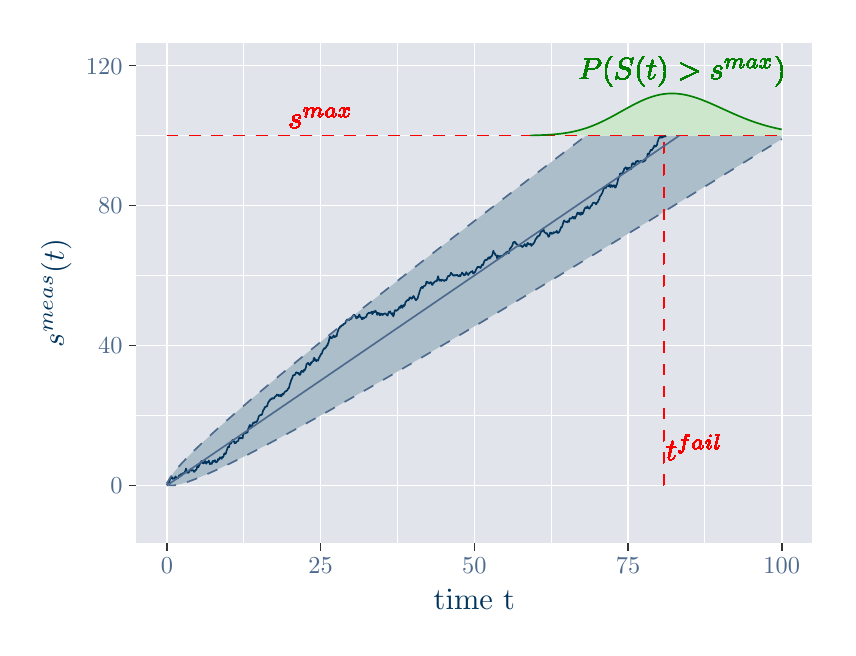
\begin{tikzpicture}[x=1pt,y=1pt]
\definecolor{fillColor}{RGB}{255,255,255}
\path[use as bounding box,fill=fillColor,fill opacity=0.00] (0,0) rectangle (289.08,216.81);
\begin{scope}
\path[clip] (  0.00,  0.00) rectangle (289.08,216.81);
\definecolor{drawColor}{RGB}{255,255,255}
\definecolor{fillColor}{RGB}{255,255,255}

\path[draw=drawColor,line width= 0.6pt,line join=round,line cap=round,fill=fillColor] (  0.00,  0.00) rectangle (289.08,216.81);
\end{scope}
\begin{scope}
\path[clip] ( 39.22, 30.56) rectangle (283.58,211.31);
\definecolor{fillColor}{RGB}{225,229,235}

\path[fill=fillColor] ( 39.22, 30.56) rectangle (283.58,211.31);
\definecolor{drawColor}{RGB}{255,255,255}

\path[draw=drawColor,line width= 0.3pt,line join=round] ( 39.22, 76.69) --
	(283.58, 76.69);

\path[draw=drawColor,line width= 0.3pt,line join=round] ( 39.22,127.25) --
	(283.58,127.25);

\path[draw=drawColor,line width= 0.3pt,line join=round] ( 39.22,177.81) --
	(283.58,177.81);

\path[draw=drawColor,line width= 0.3pt,line join=round] ( 78.10, 30.56) --
	( 78.10,211.31);

\path[draw=drawColor,line width= 0.3pt,line join=round] (133.63, 30.56) --
	(133.63,211.31);

\path[draw=drawColor,line width= 0.3pt,line join=round] (189.17, 30.56) --
	(189.17,211.31);

\path[draw=drawColor,line width= 0.3pt,line join=round] (244.70, 30.56) --
	(244.70,211.31);

\path[draw=drawColor,line width= 0.6pt,line join=round] ( 39.22, 51.41) --
	(283.58, 51.41);

\path[draw=drawColor,line width= 0.6pt,line join=round] ( 39.22,101.97) --
	(283.58,101.97);

\path[draw=drawColor,line width= 0.6pt,line join=round] ( 39.22,152.53) --
	(283.58,152.53);

\path[draw=drawColor,line width= 0.6pt,line join=round] ( 39.22,203.09) --
	(283.58,203.09);

\path[draw=drawColor,line width= 0.6pt,line join=round] ( 50.33, 30.56) --
	( 50.33,211.31);

\path[draw=drawColor,line width= 0.6pt,line join=round] (105.87, 30.56) --
	(105.87,211.31);

\path[draw=drawColor,line width= 0.6pt,line join=round] (161.40, 30.56) --
	(161.40,211.31);

\path[draw=drawColor,line width= 0.6pt,line join=round] (216.94, 30.56) --
	(216.94,211.31);

\path[draw=drawColor,line width= 0.6pt,line join=round] (272.47, 30.56) --
	(272.47,211.31);
\definecolor{fillColor}{RGB}{173,190,203}

\path[fill=fillColor] ( 50.33, 51.41) --
	( 50.55, 52.45) --
	( 50.77, 52.96) --
	( 51.00, 53.39) --
	( 51.22, 53.78) --
	( 51.44, 54.14) --
	( 51.66, 54.48) --
	( 51.88, 54.80) --
	( 52.11, 55.12) --
	( 52.33, 55.42) --
	( 52.55, 55.71) --
	( 52.77, 56.00) --
	( 53.00, 56.28) --
	( 53.22, 56.56) --
	( 53.44, 56.83) --
	( 53.66, 57.10) --
	( 53.88, 57.36) --
	( 54.11, 57.62) --
	( 54.33, 57.88) --
	( 54.55, 58.13) --
	( 54.77, 58.38) --
	( 54.99, 58.63) --
	( 55.22, 58.88) --
	( 55.44, 59.12) --
	( 55.66, 59.36) --
	( 55.88, 59.60) --
	( 56.11, 59.84) --
	( 56.33, 60.08) --
	( 56.55, 60.31) --
	( 56.77, 60.55) --
	( 56.99, 60.78) --
	( 57.22, 61.01) --
	( 57.44, 61.24) --
	( 57.66, 61.47) --
	( 57.88, 61.70) --
	( 58.10, 61.93) --
	( 58.33, 62.15) --
	( 58.55, 62.38) --
	( 58.77, 62.60) --
	( 58.99, 62.82) --
	( 59.22, 63.04) --
	( 59.44, 63.26) --
	( 59.66, 63.48) --
	( 59.88, 63.70) --
	( 60.10, 63.92) --
	( 60.33, 64.14) --
	( 60.55, 64.36) --
	( 60.77, 64.57) --
	( 60.99, 64.79) --
	( 61.21, 65.00) --
	( 61.44, 65.22) --
	( 61.66, 65.43) --
	( 61.88, 65.64) --
	( 62.10, 65.86) --
	( 62.33, 66.07) --
	( 62.55, 66.28) --
	( 62.77, 66.49) --
	( 62.99, 66.70) --
	( 63.21, 66.91) --
	( 63.44, 67.12) --
	( 63.66, 67.33) --
	( 63.88, 67.54) --
	( 64.10, 67.74) --
	( 64.32, 67.95) --
	( 64.55, 68.16) --
	( 64.77, 68.36) --
	( 64.99, 68.57) --
	( 65.21, 68.78) --
	( 65.44, 68.98) --
	( 65.66, 69.19) --
	( 65.88, 69.39) --
	( 66.10, 69.59) --
	( 66.32, 69.80) --
	( 66.55, 70.00) --
	( 66.77, 70.20) --
	( 66.99, 70.41) --
	( 67.21, 70.61) --
	( 67.43, 70.81) --
	( 67.66, 71.01) --
	( 67.88, 71.21) --
	( 68.10, 71.41) --
	( 68.32, 71.61) --
	( 68.55, 71.82) --
	( 68.77, 72.02) --
	( 68.99, 72.22) --
	( 69.21, 72.41) --
	( 69.43, 72.61) --
	( 69.66, 72.81) --
	( 69.88, 73.01) --
	( 70.10, 73.21) --
	( 70.32, 73.41) --
	( 70.54, 73.61) --
	( 70.77, 73.80) --
	( 70.99, 74.00) --
	( 71.21, 74.20) --
	( 71.43, 74.40) --
	( 71.66, 74.59) --
	( 71.88, 74.79) --
	( 72.10, 74.98) --
	( 72.32, 75.18) --
	( 72.54, 75.38) --
	( 72.77, 75.57) --
	( 72.99, 75.77) --
	( 73.21, 75.96) --
	( 73.43, 76.16) --
	( 73.65, 76.35) --
	( 73.88, 76.55) --
	( 74.10, 76.74) --
	( 74.32, 76.93) --
	( 74.54, 77.13) --
	( 74.77, 77.32) --
	( 74.99, 77.52) --
	( 75.21, 77.71) --
	( 75.43, 77.90) --
	( 75.65, 78.10) --
	( 75.88, 78.29) --
	( 76.10, 78.48) --
	( 76.32, 78.67) --
	( 76.54, 78.87) --
	( 76.76, 79.06) --
	( 76.99, 79.25) --
	( 77.21, 79.44) --
	( 77.43, 79.63) --
	( 77.65, 79.82) --
	( 77.88, 80.02) --
	( 78.10, 80.21) --
	( 78.32, 80.40) --
	( 78.54, 80.59) --
	( 78.76, 80.78) --
	( 78.99, 80.97) --
	( 79.21, 81.16) --
	( 79.43, 81.35) --
	( 79.65, 81.54) --
	( 79.87, 81.73) --
	( 80.10, 81.92) --
	( 80.32, 82.11) --
	( 80.54, 82.30) --
	( 80.76, 82.49) --
	( 80.99, 82.68) --
	( 81.21, 82.87) --
	( 81.43, 83.05) --
	( 81.65, 83.24) --
	( 81.87, 83.43) --
	( 82.10, 83.62) --
	( 82.32, 83.81) --
	( 82.54, 84.00) --
	( 82.76, 84.19) --
	( 82.98, 84.37) --
	( 83.21, 84.56) --
	( 83.43, 84.75) --
	( 83.65, 84.94) --
	( 83.87, 85.12) --
	( 84.10, 85.31) --
	( 84.32, 85.50) --
	( 84.54, 85.69) --
	( 84.76, 85.87) --
	( 84.98, 86.06) --
	( 85.21, 86.25) --
	( 85.43, 86.43) --
	( 85.65, 86.62) --
	( 85.87, 86.81) --
	( 86.09, 86.99) --
	( 86.32, 87.18) --
	( 86.54, 87.37) --
	( 86.76, 87.55) --
	( 86.98, 87.74) --
	( 87.21, 87.92) --
	( 87.43, 88.11) --
	( 87.65, 88.29) --
	( 87.87, 88.48) --
	( 88.09, 88.67) --
	( 88.32, 88.85) --
	( 88.54, 89.04) --
	( 88.76, 89.22) --
	( 88.98, 89.41) --
	( 89.20, 89.59) --
	( 89.43, 89.78) --
	( 89.65, 89.96) --
	( 89.87, 90.15) --
	( 90.09, 90.33) --
	( 90.32, 90.51) --
	( 90.54, 90.70) --
	( 90.76, 90.88) --
	( 90.98, 91.07) --
	( 91.20, 91.25) --
	( 91.43, 91.44) --
	( 91.65, 91.62) --
	( 91.87, 91.80) --
	( 92.09, 91.99) --
	( 92.31, 92.17) --
	( 92.54, 92.35) --
	( 92.76, 92.54) --
	( 92.98, 92.72) --
	( 93.20, 92.91) --
	( 93.43, 93.09) --
	( 93.65, 93.27) --
	( 93.87, 93.45) --
	( 94.09, 93.64) --
	( 94.31, 93.82) --
	( 94.54, 94.00) --
	( 94.76, 94.19) --
	( 94.98, 94.37) --
	( 95.20, 94.55) --
	( 95.42, 94.73) --
	( 95.65, 94.92) --
	( 95.87, 95.10) --
	( 96.09, 95.28) --
	( 96.31, 95.46) --
	( 96.54, 95.65) --
	( 96.76, 95.83) --
	( 96.98, 96.01) --
	( 97.20, 96.19) --
	( 97.42, 96.37) --
	( 97.65, 96.56) --
	( 97.87, 96.74) --
	( 98.09, 96.92) --
	( 98.31, 97.10) --
	( 98.53, 97.28) --
	( 98.76, 97.46) --
	( 98.98, 97.65) --
	( 99.20, 97.83) --
	( 99.42, 98.01) --
	( 99.65, 98.19) --
	( 99.87, 98.37) --
	(100.09, 98.55) --
	(100.31, 98.73) --
	(100.53, 98.91) --
	(100.76, 99.09) --
	(100.98, 99.28) --
	(101.20, 99.46) --
	(101.42, 99.64) --
	(101.64, 99.82) --
	(101.87,100.00) --
	(102.09,100.18) --
	(102.31,100.36) --
	(102.53,100.54) --
	(102.76,100.72) --
	(102.98,100.90) --
	(103.20,101.08) --
	(103.42,101.26) --
	(103.64,101.44) --
	(103.87,101.62) --
	(104.09,101.80) --
	(104.31,101.98) --
	(104.53,102.16) --
	(104.75,102.34) --
	(104.98,102.52) --
	(105.20,102.70) --
	(105.42,102.88) --
	(105.64,103.06) --
	(105.87,103.24) --
	(106.09,103.42) --
	(106.31,103.60) --
	(106.53,103.78) --
	(106.75,103.96) --
	(106.98,104.14) --
	(107.20,104.31) --
	(107.42,104.49) --
	(107.64,104.67) --
	(107.86,104.85) --
	(108.09,105.03) --
	(108.31,105.21) --
	(108.53,105.39) --
	(108.75,105.57) --
	(108.98,105.75) --
	(109.20,105.92) --
	(109.42,106.10) --
	(109.64,106.28) --
	(109.86,106.46) --
	(110.09,106.64) --
	(110.31,106.82) --
	(110.53,107.00) --
	(110.75,107.17) --
	(110.97,107.35) --
	(111.20,107.53) --
	(111.42,107.71) --
	(111.64,107.89) --
	(111.86,108.07) --
	(112.09,108.24) --
	(112.31,108.42) --
	(112.53,108.60) --
	(112.75,108.78) --
	(112.97,108.96) --
	(113.20,109.13) --
	(113.42,109.31) --
	(113.64,109.49) --
	(113.86,109.67) --
	(114.08,109.84) --
	(114.31,110.02) --
	(114.53,110.20) --
	(114.75,110.38) --
	(114.97,110.55) --
	(115.20,110.73) --
	(115.42,110.91) --
	(115.64,111.09) --
	(115.86,111.26) --
	(116.08,111.44) --
	(116.31,111.62) --
	(116.53,111.80) --
	(116.75,111.97) --
	(116.97,112.15) --
	(117.19,112.33) --
	(117.42,112.50) --
	(117.64,112.68) --
	(117.86,112.86) --
	(118.08,113.03) --
	(118.31,113.21) --
	(118.53,113.39) --
	(118.75,113.56) --
	(118.97,113.74) --
	(119.19,113.92) --
	(119.42,114.09) --
	(119.64,114.27) --
	(119.86,114.45) --
	(120.08,114.62) --
	(120.30,114.80) --
	(120.53,114.98) --
	(120.75,115.15) --
	(120.97,115.33) --
	(121.19,115.51) --
	(121.42,115.68) --
	(121.64,115.86) --
	(121.86,116.04) --
	(122.08,116.21) --
	(122.30,116.39) --
	(122.53,116.56) --
	(122.75,116.74) --
	(122.97,116.92) --
	(123.19,117.09) --
	(123.41,117.27) --
	(123.64,117.44) --
	(123.86,117.62) --
	(124.08,117.79) --
	(124.30,117.97) --
	(124.53,118.15) --
	(124.75,118.32) --
	(124.97,118.50) --
	(125.19,118.67) --
	(125.41,118.85) --
	(125.64,119.02) --
	(125.86,119.20) --
	(126.08,119.38) --
	(126.30,119.55) --
	(126.52,119.73) --
	(126.75,119.90) --
	(126.97,120.08) --
	(127.19,120.25) --
	(127.41,120.43) --
	(127.64,120.60) --
	(127.86,120.78) --
	(128.08,120.95) --
	(128.30,121.13) --
	(128.52,121.30) --
	(128.75,121.48) --
	(128.97,121.65) --
	(129.19,121.83) --
	(129.41,122.00) --
	(129.63,122.18) --
	(129.86,122.35) --
	(130.08,122.53) --
	(130.30,122.70) --
	(130.52,122.88) --
	(130.75,123.05) --
	(130.97,123.23) --
	(131.19,123.40) --
	(131.41,123.58) --
	(131.63,123.75) --
	(131.86,123.93) --
	(132.08,124.10) --
	(132.30,124.28) --
	(132.52,124.45) --
	(132.74,124.63) --
	(132.97,124.80) --
	(133.19,124.97) --
	(133.41,125.15) --
	(133.63,125.32) --
	(133.86,125.50) --
	(134.08,125.67) --
	(134.30,125.85) --
	(134.52,126.02) --
	(134.74,126.19) --
	(134.97,126.37) --
	(135.19,126.54) --
	(135.41,126.72) --
	(135.63,126.89) --
	(135.85,127.07) --
	(136.08,127.24) --
	(136.30,127.41) --
	(136.52,127.59) --
	(136.74,127.76) --
	(136.97,127.94) --
	(137.19,128.11) --
	(137.41,128.28) --
	(137.63,128.46) --
	(137.85,128.63) --
	(138.08,128.80) --
	(138.30,128.98) --
	(138.52,129.15) --
	(138.74,129.33) --
	(138.96,129.50) --
	(139.19,129.67) --
	(139.41,129.85) --
	(139.63,130.02) --
	(139.85,130.19) --
	(140.08,130.37) --
	(140.30,130.54) --
	(140.52,130.72) --
	(140.74,130.89) --
	(140.96,131.06) --
	(141.19,131.24) --
	(141.41,131.41) --
	(141.63,131.58) --
	(141.85,131.76) --
	(142.07,131.93) --
	(142.30,132.10) --
	(142.52,132.28) --
	(142.74,132.45) --
	(142.96,132.62) --
	(143.19,132.80) --
	(143.41,132.97) --
	(143.63,133.14) --
	(143.85,133.31) --
	(144.07,133.49) --
	(144.30,133.66) --
	(144.52,133.83) --
	(144.74,134.01) --
	(144.96,134.18) --
	(145.18,134.35) --
	(145.41,134.53) --
	(145.63,134.70) --
	(145.85,134.87) --
	(146.07,135.04) --
	(146.30,135.22) --
	(146.52,135.39) --
	(146.74,135.56) --
	(146.96,135.74) --
	(147.18,135.91) --
	(147.41,136.08) --
	(147.63,136.25) --
	(147.85,136.43) --
	(148.07,136.60) --
	(148.29,136.77) --
	(148.52,136.94) --
	(148.74,137.12) --
	(148.96,137.29) --
	(149.18,137.46) --
	(149.41,137.63) --
	(149.63,137.81) --
	(149.85,137.98) --
	(150.07,138.15) --
	(150.29,138.32) --
	(150.52,138.50) --
	(150.74,138.67) --
	(150.96,138.84) --
	(151.18,139.01) --
	(151.40,139.19) --
	(151.63,139.36) --
	(151.85,139.53) --
	(152.07,139.70) --
	(152.29,139.88) --
	(152.52,140.05) --
	(152.74,140.22) --
	(152.96,140.39) --
	(153.18,140.56) --
	(153.40,140.74) --
	(153.63,140.91) --
	(153.85,141.08) --
	(154.07,141.25) --
	(154.29,141.42) --
	(154.51,141.60) --
	(154.74,141.77) --
	(154.96,141.94) --
	(155.18,142.11) --
	(155.40,142.28) --
	(155.63,142.46) --
	(155.85,142.63) --
	(156.07,142.80) --
	(156.29,142.97) --
	(156.51,143.14) --
	(156.74,143.31) --
	(156.96,143.49) --
	(157.18,143.66) --
	(157.40,143.83) --
	(157.62,144.00) --
	(157.85,144.17) --
	(158.07,144.35) --
	(158.29,144.52) --
	(158.51,144.69) --
	(158.74,144.86) --
	(158.96,145.03) --
	(159.18,145.20) --
	(159.40,145.37) --
	(159.62,145.55) --
	(159.85,145.72) --
	(160.07,145.89) --
	(160.29,146.06) --
	(160.51,146.23) --
	(160.73,146.40) --
	(160.96,146.57) --
	(161.18,146.75) --
	(161.40,146.92) --
	(161.62,147.09) --
	(161.85,147.26) --
	(162.07,147.43) --
	(162.29,147.60) --
	(162.51,147.77) --
	(162.73,147.95) --
	(162.96,148.12) --
	(163.18,148.29) --
	(163.40,148.46) --
	(163.62,148.63) --
	(163.84,148.80) --
	(164.07,148.97) --
	(164.29,149.14) --
	(164.51,149.31) --
	(164.73,149.49) --
	(164.96,149.66) --
	(165.18,149.83) --
	(165.40,150.00) --
	(165.62,150.17) --
	(165.84,150.34) --
	(166.07,150.51) --
	(166.29,150.68) --
	(166.51,150.85) --
	(166.73,151.02) --
	(166.95,151.20) --
	(167.18,151.37) --
	(167.40,151.54) --
	(167.62,151.71) --
	(167.84,151.88) --
	(168.07,152.05) --
	(168.29,152.22) --
	(168.51,152.39) --
	(168.73,152.56) --
	(168.95,152.73) --
	(169.18,152.90) --
	(169.40,153.07) --
	(169.62,153.24) --
	(169.84,153.41) --
	(170.06,153.59) --
	(170.29,153.76) --
	(170.51,153.93) --
	(170.73,154.10) --
	(170.95,154.27) --
	(171.18,154.44) --
	(171.40,154.61) --
	(171.62,154.78) --
	(171.84,154.95) --
	(172.06,155.12) --
	(172.29,155.29) --
	(172.51,155.46) --
	(172.73,155.63) --
	(172.95,155.80) --
	(173.17,155.97) --
	(173.40,156.14) --
	(173.62,156.31) --
	(173.84,156.48) --
	(174.06,156.65) --
	(174.29,156.82) --
	(174.51,156.99) --
	(174.73,157.16) --
	(174.95,157.33) --
	(175.17,157.51) --
	(175.40,157.68) --
	(175.62,157.85) --
	(175.84,158.02) --
	(176.06,158.19) --
	(176.28,158.36) --
	(176.51,158.53) --
	(176.73,158.70) --
	(176.95,158.87) --
	(177.17,159.04) --
	(177.40,159.21) --
	(177.62,159.38) --
	(177.84,159.55) --
	(178.06,159.72) --
	(178.28,159.89) --
	(178.51,160.06) --
	(178.73,160.23) --
	(178.95,160.40) --
	(179.17,160.57) --
	(179.39,160.74) --
	(179.62,160.91) --
	(179.84,161.08) --
	(180.06,161.25) --
	(180.28,161.42) --
	(180.51,161.59) --
	(180.73,161.76) --
	(180.95,161.93) --
	(181.17,162.10) --
	(181.39,162.27) --
	(181.62,162.43) --
	(181.84,162.60) --
	(182.06,162.77) --
	(182.28,162.94) --
	(182.50,163.11) --
	(182.73,163.28) --
	(182.95,163.45) --
	(183.17,163.62) --
	(183.39,163.79) --
	(183.62,163.96) --
	(183.84,164.13) --
	(184.06,164.30) --
	(184.28,164.47) --
	(184.50,164.64) --
	(184.73,164.81) --
	(184.95,164.98) --
	(185.17,165.15) --
	(185.39,165.32) --
	(185.61,165.49) --
	(185.84,165.66) --
	(186.06,165.83) --
	(186.28,166.00) --
	(186.50,166.17) --
	(186.73,166.34) --
	(186.95,166.50) --
	(187.17,166.67) --
	(187.39,166.84) --
	(187.61,167.01) --
	(187.84,167.18) --
	(188.06,167.35) --
	(188.28,167.52) --
	(188.50,167.69) --
	(188.72,167.86) --
	(188.95,168.03) --
	(189.17,168.20) --
	(189.39,168.37) --
	(189.61,168.54) --
	(189.84,168.71) --
	(190.06,168.88) --
	(190.28,169.04) --
	(190.50,169.21) --
	(190.72,169.38) --
	(190.95,169.55) --
	(191.17,169.72) --
	(191.39,169.89) --
	(191.61,170.06) --
	(191.83,170.23) --
	(192.06,170.40) --
	(192.28,170.57) --
	(192.50,170.74) --
	(192.72,170.90) --
	(192.95,171.07) --
	(193.17,171.24) --
	(193.39,171.41) --
	(193.61,171.58) --
	(193.83,171.75) --
	(194.06,171.92) --
	(194.28,172.09) --
	(194.50,172.26) --
	(194.72,172.43) --
	(194.94,172.59) --
	(195.17,172.76) --
	(195.39,172.93) --
	(195.61,173.10) --
	(195.83,173.27) --
	(196.06,173.44) --
	(196.28,173.61) --
	(196.50,173.78) --
	(196.72,173.95) --
	(196.94,174.11) --
	(197.17,174.28) --
	(197.39,174.45) --
	(197.61,174.62) --
	(197.83,174.79) --
	(198.05,174.96) --
	(198.28,175.13) --
	(198.50,175.30) --
	(198.72,175.46) --
	(198.94,175.63) --
	(199.17,175.80) --
	(199.39,175.97) --
	(199.61,176.14) --
	(199.83,176.31) --
	(200.05,176.48) --
	(200.28,176.64) --
	(200.50,176.81) --
	(200.72,176.98) --
	(200.94,177.15) --
	(201.16,177.32) --
	(201.39,177.49) --
	(201.61,177.66) --
	(201.83,177.81) --
	(202.05,177.81) --
	(202.28,177.81) --
	(202.50,177.81) --
	(202.72,177.81) --
	(202.94,177.81) --
	(203.16,177.81) --
	(203.39,177.81) --
	(203.61,177.81) --
	(203.83,177.81) --
	(204.05,177.81) --
	(204.27,177.81) --
	(204.50,177.81) --
	(204.72,177.81) --
	(204.94,177.81) --
	(205.16,177.81) --
	(205.39,177.81) --
	(205.61,177.81) --
	(205.83,177.81) --
	(206.05,177.81) --
	(206.27,177.81) --
	(206.50,177.81) --
	(206.72,177.81) --
	(206.94,177.81) --
	(207.16,177.81) --
	(207.38,177.81) --
	(207.61,177.81) --
	(207.83,177.81) --
	(208.05,177.81) --
	(208.27,177.81) --
	(208.50,177.81) --
	(208.72,177.81) --
	(208.94,177.81) --
	(209.16,177.81) --
	(209.38,177.81) --
	(209.61,177.81) --
	(209.83,177.81) --
	(210.05,177.81) --
	(210.27,177.81) --
	(210.49,177.81) --
	(210.72,177.81) --
	(210.94,177.81) --
	(211.16,177.81) --
	(211.38,177.81) --
	(211.61,177.81) --
	(211.83,177.81) --
	(212.05,177.81) --
	(212.27,177.81) --
	(212.49,177.81) --
	(212.72,177.81) --
	(212.94,177.81) --
	(213.16,177.81) --
	(213.38,177.81) --
	(213.60,177.81) --
	(213.83,177.81) --
	(214.05,177.81) --
	(214.27,177.81) --
	(214.49,177.81) --
	(214.72,177.81) --
	(214.94,177.81) --
	(215.16,177.81) --
	(215.38,177.81) --
	(215.60,177.81) --
	(215.83,177.81) --
	(216.05,177.81) --
	(216.27,177.81) --
	(216.49,177.81) --
	(216.71,177.81) --
	(216.94,177.81) --
	(217.16,177.81) --
	(217.38,177.81) --
	(217.60,177.81) --
	(217.83,177.81) --
	(218.05,177.81) --
	(218.27,177.81) --
	(218.49,177.81) --
	(218.71,177.81) --
	(218.94,177.81) --
	(219.16,177.81) --
	(219.38,177.81) --
	(219.60,177.81) --
	(219.82,177.81) --
	(220.05,177.81) --
	(220.27,177.81) --
	(220.49,177.81) --
	(220.71,177.81) --
	(220.94,177.81) --
	(221.16,177.81) --
	(221.38,177.81) --
	(221.60,177.81) --
	(221.82,177.81) --
	(222.05,177.81) --
	(222.27,177.81) --
	(222.49,177.81) --
	(222.71,177.81) --
	(222.93,177.81) --
	(223.16,177.81) --
	(223.38,177.81) --
	(223.60,177.81) --
	(223.82,177.81) --
	(224.05,177.81) --
	(224.27,177.81) --
	(224.49,177.81) --
	(224.71,177.81) --
	(224.93,177.81) --
	(225.16,177.81) --
	(225.38,177.81) --
	(225.60,177.81) --
	(225.82,177.81) --
	(226.04,177.81) --
	(226.27,177.81) --
	(226.49,177.81) --
	(226.71,177.81) --
	(226.93,177.81) --
	(227.16,177.81) --
	(227.38,177.81) --
	(227.60,177.81) --
	(227.82,177.81) --
	(228.04,177.81) --
	(228.27,177.81) --
	(228.49,177.81) --
	(228.71,177.81) --
	(228.93,177.81) --
	(229.15,177.81) --
	(229.38,177.81) --
	(229.60,177.81) --
	(229.82,177.81) --
	(230.04,177.81) --
	(230.27,177.81) --
	(230.49,177.81) --
	(230.71,177.81) --
	(230.93,177.81) --
	(231.15,177.81) --
	(231.38,177.81) --
	(231.60,177.81) --
	(231.82,177.81) --
	(232.04,177.81) --
	(232.26,177.81) --
	(232.49,177.81) --
	(232.71,177.81) --
	(232.93,177.81) --
	(233.15,177.81) --
	(233.38,177.81) --
	(233.60,177.81) --
	(233.82,177.81) --
	(234.04,177.81) --
	(234.26,177.81) --
	(234.49,177.81) --
	(234.71,177.81) --
	(234.93,177.81) --
	(235.15,177.81) --
	(235.37,177.81) --
	(235.60,177.81) --
	(235.82,177.81) --
	(236.04,177.81) --
	(236.26,177.81) --
	(236.49,177.81) --
	(236.71,177.81) --
	(236.93,177.81) --
	(237.15,177.81) --
	(237.37,177.81) --
	(237.60,177.81) --
	(237.82,177.81) --
	(238.04,177.81) --
	(238.26,177.81) --
	(238.48,177.81) --
	(238.71,177.81) --
	(238.93,177.81) --
	(239.15,177.81) --
	(239.37,177.81) --
	(239.60,177.81) --
	(239.82,177.81) --
	(240.04,177.81) --
	(240.26,177.81) --
	(240.48,177.81) --
	(240.71,177.81) --
	(240.93,177.81) --
	(241.15,177.81) --
	(241.37,177.81) --
	(241.59,177.81) --
	(241.82,177.81) --
	(242.04,177.81) --
	(242.26,177.81) --
	(242.48,177.81) --
	(242.71,177.81) --
	(242.93,177.81) --
	(243.15,177.81) --
	(243.37,177.81) --
	(243.59,177.81) --
	(243.82,177.81) --
	(244.04,177.81) --
	(244.26,177.81) --
	(244.48,177.81) --
	(244.70,177.81) --
	(244.93,177.81) --
	(245.15,177.81) --
	(245.37,177.81) --
	(245.59,177.81) --
	(245.82,177.81) --
	(246.04,177.81) --
	(246.26,177.81) --
	(246.48,177.81) --
	(246.70,177.81) --
	(246.93,177.81) --
	(247.15,177.81) --
	(247.37,177.81) --
	(247.59,177.81) --
	(247.81,177.81) --
	(248.04,177.81) --
	(248.26,177.81) --
	(248.48,177.81) --
	(248.70,177.81) --
	(248.93,177.81) --
	(249.15,177.81) --
	(249.37,177.81) --
	(249.59,177.81) --
	(249.81,177.81) --
	(250.04,177.81) --
	(250.26,177.81) --
	(250.48,177.81) --
	(250.70,177.81) --
	(250.92,177.81) --
	(251.15,177.81) --
	(251.37,177.81) --
	(251.59,177.81) --
	(251.81,177.81) --
	(252.04,177.81) --
	(252.26,177.81) --
	(252.48,177.81) --
	(252.70,177.81) --
	(252.92,177.81) --
	(253.15,177.81) --
	(253.37,177.81) --
	(253.59,177.81) --
	(253.81,177.81) --
	(254.03,177.81) --
	(254.26,177.81) --
	(254.48,177.81) --
	(254.70,177.81) --
	(254.92,177.81) --
	(255.15,177.81) --
	(255.37,177.81) --
	(255.59,177.81) --
	(255.81,177.81) --
	(256.03,177.81) --
	(256.26,177.81) --
	(256.48,177.81) --
	(256.70,177.81) --
	(256.92,177.81) --
	(257.14,177.81) --
	(257.37,177.81) --
	(257.59,177.81) --
	(257.81,177.81) --
	(258.03,177.81) --
	(258.26,177.81) --
	(258.48,177.81) --
	(258.70,177.81) --
	(258.92,177.81) --
	(259.14,177.81) --
	(259.37,177.81) --
	(259.59,177.81) --
	(259.81,177.81) --
	(260.03,177.81) --
	(260.25,177.81) --
	(260.48,177.81) --
	(260.70,177.81) --
	(260.92,177.81) --
	(261.14,177.81) --
	(261.37,177.81) --
	(261.59,177.81) --
	(261.81,177.81) --
	(262.03,177.81) --
	(262.25,177.81) --
	(262.48,177.81) --
	(262.70,177.81) --
	(262.92,177.81) --
	(263.14,177.81) --
	(263.36,177.81) --
	(263.59,177.81) --
	(263.81,177.81) --
	(264.03,177.81) --
	(264.25,177.81) --
	(264.48,177.81) --
	(264.70,177.81) --
	(264.92,177.81) --
	(265.14,177.81) --
	(265.36,177.81) --
	(265.59,177.81) --
	(265.81,177.81) --
	(266.03,177.81) --
	(266.25,177.81) --
	(266.47,177.81) --
	(266.70,177.81) --
	(266.92,177.81) --
	(267.14,177.81) --
	(267.36,177.81) --
	(267.59,177.81) --
	(267.81,177.81) --
	(268.03,177.81) --
	(268.25,177.81) --
	(268.47,177.81) --
	(268.70,177.81) --
	(268.92,177.81) --
	(269.14,177.81) --
	(269.36,177.81) --
	(269.58,177.81) --
	(269.81,177.81) --
	(270.03,177.81) --
	(270.25,177.81) --
	(270.47,177.81) --
	(270.70,177.81) --
	(270.92,177.81) --
	(271.14,177.81) --
	(271.36,177.81) --
	(271.58,177.81) --
	(271.81,177.81) --
	(272.03,177.81) --
	(272.25,177.81) --
	(272.47,177.81) --
	(272.47,176.56) --
	(272.25,176.42) --
	(272.03,176.28) --
	(271.81,176.15) --
	(271.58,176.01) --
	(271.36,175.87) --
	(271.14,175.73) --
	(270.92,175.60) --
	(270.70,175.46) --
	(270.47,175.32) --
	(270.25,175.18) --
	(270.03,175.04) --
	(269.81,174.91) --
	(269.58,174.77) --
	(269.36,174.63) --
	(269.14,174.49) --
	(268.92,174.36) --
	(268.70,174.22) --
	(268.47,174.08) --
	(268.25,173.94) --
	(268.03,173.81) --
	(267.81,173.67) --
	(267.59,173.53) --
	(267.36,173.39) --
	(267.14,173.26) --
	(266.92,173.12) --
	(266.70,172.98) --
	(266.47,172.84) --
	(266.25,172.70) --
	(266.03,172.57) --
	(265.81,172.43) --
	(265.59,172.29) --
	(265.36,172.15) --
	(265.14,172.02) --
	(264.92,171.88) --
	(264.70,171.74) --
	(264.48,171.60) --
	(264.25,171.47) --
	(264.03,171.33) --
	(263.81,171.19) --
	(263.59,171.05) --
	(263.36,170.92) --
	(263.14,170.78) --
	(262.92,170.64) --
	(262.70,170.50) --
	(262.48,170.37) --
	(262.25,170.23) --
	(262.03,170.09) --
	(261.81,169.95) --
	(261.59,169.82) --
	(261.37,169.68) --
	(261.14,169.54) --
	(260.92,169.41) --
	(260.70,169.27) --
	(260.48,169.13) --
	(260.25,168.99) --
	(260.03,168.86) --
	(259.81,168.72) --
	(259.59,168.58) --
	(259.37,168.44) --
	(259.14,168.31) --
	(258.92,168.17) --
	(258.70,168.03) --
	(258.48,167.89) --
	(258.26,167.76) --
	(258.03,167.62) --
	(257.81,167.48) --
	(257.59,167.35) --
	(257.37,167.21) --
	(257.14,167.07) --
	(256.92,166.93) --
	(256.70,166.80) --
	(256.48,166.66) --
	(256.26,166.52) --
	(256.03,166.38) --
	(255.81,166.25) --
	(255.59,166.11) --
	(255.37,165.97) --
	(255.15,165.84) --
	(254.92,165.70) --
	(254.70,165.56) --
	(254.48,165.42) --
	(254.26,165.29) --
	(254.03,165.15) --
	(253.81,165.01) --
	(253.59,164.88) --
	(253.37,164.74) --
	(253.15,164.60) --
	(252.92,164.46) --
	(252.70,164.33) --
	(252.48,164.19) --
	(252.26,164.05) --
	(252.04,163.92) --
	(251.81,163.78) --
	(251.59,163.64) --
	(251.37,163.50) --
	(251.15,163.37) --
	(250.92,163.23) --
	(250.70,163.09) --
	(250.48,162.96) --
	(250.26,162.82) --
	(250.04,162.68) --
	(249.81,162.54) --
	(249.59,162.41) --
	(249.37,162.27) --
	(249.15,162.13) --
	(248.93,162.00) --
	(248.70,161.86) --
	(248.48,161.72) --
	(248.26,161.59) --
	(248.04,161.45) --
	(247.81,161.31) --
	(247.59,161.18) --
	(247.37,161.04) --
	(247.15,160.90) --
	(246.93,160.76) --
	(246.70,160.63) --
	(246.48,160.49) --
	(246.26,160.35) --
	(246.04,160.22) --
	(245.82,160.08) --
	(245.59,159.94) --
	(245.37,159.81) --
	(245.15,159.67) --
	(244.93,159.53) --
	(244.70,159.40) --
	(244.48,159.26) --
	(244.26,159.12) --
	(244.04,158.99) --
	(243.82,158.85) --
	(243.59,158.71) --
	(243.37,158.58) --
	(243.15,158.44) --
	(242.93,158.30) --
	(242.71,158.16) --
	(242.48,158.03) --
	(242.26,157.89) --
	(242.04,157.75) --
	(241.82,157.62) --
	(241.59,157.48) --
	(241.37,157.34) --
	(241.15,157.21) --
	(240.93,157.07) --
	(240.71,156.93) --
	(240.48,156.80) --
	(240.26,156.66) --
	(240.04,156.52) --
	(239.82,156.39) --
	(239.60,156.25) --
	(239.37,156.11) --
	(239.15,155.98) --
	(238.93,155.84) --
	(238.71,155.71) --
	(238.48,155.57) --
	(238.26,155.43) --
	(238.04,155.30) --
	(237.82,155.16) --
	(237.60,155.02) --
	(237.37,154.89) --
	(237.15,154.75) --
	(236.93,154.61) --
	(236.71,154.48) --
	(236.49,154.34) --
	(236.26,154.20) --
	(236.04,154.07) --
	(235.82,153.93) --
	(235.60,153.79) --
	(235.37,153.66) --
	(235.15,153.52) --
	(234.93,153.38) --
	(234.71,153.25) --
	(234.49,153.11) --
	(234.26,152.98) --
	(234.04,152.84) --
	(233.82,152.70) --
	(233.60,152.57) --
	(233.38,152.43) --
	(233.15,152.29) --
	(232.93,152.16) --
	(232.71,152.02) --
	(232.49,151.88) --
	(232.26,151.75) --
	(232.04,151.61) --
	(231.82,151.48) --
	(231.60,151.34) --
	(231.38,151.20) --
	(231.15,151.07) --
	(230.93,150.93) --
	(230.71,150.79) --
	(230.49,150.66) --
	(230.27,150.52) --
	(230.04,150.39) --
	(229.82,150.25) --
	(229.60,150.11) --
	(229.38,149.98) --
	(229.15,149.84) --
	(228.93,149.70) --
	(228.71,149.57) --
	(228.49,149.43) --
	(228.27,149.30) --
	(228.04,149.16) --
	(227.82,149.02) --
	(227.60,148.89) --
	(227.38,148.75) --
	(227.16,148.62) --
	(226.93,148.48) --
	(226.71,148.34) --
	(226.49,148.21) --
	(226.27,148.07) --
	(226.04,147.93) --
	(225.82,147.80) --
	(225.60,147.66) --
	(225.38,147.53) --
	(225.16,147.39) --
	(224.93,147.25) --
	(224.71,147.12) --
	(224.49,146.98) --
	(224.27,146.85) --
	(224.05,146.71) --
	(223.82,146.58) --
	(223.60,146.44) --
	(223.38,146.30) --
	(223.16,146.17) --
	(222.93,146.03) --
	(222.71,145.90) --
	(222.49,145.76) --
	(222.27,145.62) --
	(222.05,145.49) --
	(221.82,145.35) --
	(221.60,145.22) --
	(221.38,145.08) --
	(221.16,144.94) --
	(220.94,144.81) --
	(220.71,144.67) --
	(220.49,144.54) --
	(220.27,144.40) --
	(220.05,144.27) --
	(219.82,144.13) --
	(219.60,143.99) --
	(219.38,143.86) --
	(219.16,143.72) --
	(218.94,143.59) --
	(218.71,143.45) --
	(218.49,143.32) --
	(218.27,143.18) --
	(218.05,143.04) --
	(217.83,142.91) --
	(217.60,142.77) --
	(217.38,142.64) --
	(217.16,142.50) --
	(216.94,142.37) --
	(216.71,142.23) --
	(216.49,142.09) --
	(216.27,141.96) --
	(216.05,141.82) --
	(215.83,141.69) --
	(215.60,141.55) --
	(215.38,141.42) --
	(215.16,141.28) --
	(214.94,141.15) --
	(214.72,141.01) --
	(214.49,140.87) --
	(214.27,140.74) --
	(214.05,140.60) --
	(213.83,140.47) --
	(213.60,140.33) --
	(213.38,140.20) --
	(213.16,140.06) --
	(212.94,139.93) --
	(212.72,139.79) --
	(212.49,139.66) --
	(212.27,139.52) --
	(212.05,139.38) --
	(211.83,139.25) --
	(211.61,139.11) --
	(211.38,138.98) --
	(211.16,138.84) --
	(210.94,138.71) --
	(210.72,138.57) --
	(210.49,138.44) --
	(210.27,138.30) --
	(210.05,138.17) --
	(209.83,138.03) --
	(209.61,137.90) --
	(209.38,137.76) --
	(209.16,137.63) --
	(208.94,137.49) --
	(208.72,137.36) --
	(208.50,137.22) --
	(208.27,137.08) --
	(208.05,136.95) --
	(207.83,136.81) --
	(207.61,136.68) --
	(207.38,136.54) --
	(207.16,136.41) --
	(206.94,136.27) --
	(206.72,136.14) --
	(206.50,136.00) --
	(206.27,135.87) --
	(206.05,135.73) --
	(205.83,135.60) --
	(205.61,135.46) --
	(205.39,135.33) --
	(205.16,135.19) --
	(204.94,135.06) --
	(204.72,134.92) --
	(204.50,134.79) --
	(204.27,134.65) --
	(204.05,134.52) --
	(203.83,134.38) --
	(203.61,134.25) --
	(203.39,134.11) --
	(203.16,133.98) --
	(202.94,133.84) --
	(202.72,133.71) --
	(202.50,133.57) --
	(202.28,133.44) --
	(202.05,133.30) --
	(201.83,133.17) --
	(201.61,133.03) --
	(201.39,132.90) --
	(201.16,132.76) --
	(200.94,132.63) --
	(200.72,132.50) --
	(200.50,132.36) --
	(200.28,132.23) --
	(200.05,132.09) --
	(199.83,131.96) --
	(199.61,131.82) --
	(199.39,131.69) --
	(199.17,131.55) --
	(198.94,131.42) --
	(198.72,131.28) --
	(198.50,131.15) --
	(198.28,131.01) --
	(198.05,130.88) --
	(197.83,130.74) --
	(197.61,130.61) --
	(197.39,130.47) --
	(197.17,130.34) --
	(196.94,130.21) --
	(196.72,130.07) --
	(196.50,129.94) --
	(196.28,129.80) --
	(196.06,129.67) --
	(195.83,129.53) --
	(195.61,129.40) --
	(195.39,129.26) --
	(195.17,129.13) --
	(194.94,129.00) --
	(194.72,128.86) --
	(194.50,128.73) --
	(194.28,128.59) --
	(194.06,128.46) --
	(193.83,128.32) --
	(193.61,128.19) --
	(193.39,128.05) --
	(193.17,127.92) --
	(192.95,127.79) --
	(192.72,127.65) --
	(192.50,127.52) --
	(192.28,127.38) --
	(192.06,127.25) --
	(191.83,127.11) --
	(191.61,126.98) --
	(191.39,126.85) --
	(191.17,126.71) --
	(190.95,126.58) --
	(190.72,126.44) --
	(190.50,126.31) --
	(190.28,126.17) --
	(190.06,126.04) --
	(189.84,125.91) --
	(189.61,125.77) --
	(189.39,125.64) --
	(189.17,125.50) --
	(188.95,125.37) --
	(188.72,125.24) --
	(188.50,125.10) --
	(188.28,124.97) --
	(188.06,124.83) --
	(187.84,124.70) --
	(187.61,124.57) --
	(187.39,124.43) --
	(187.17,124.30) --
	(186.95,124.16) --
	(186.73,124.03) --
	(186.50,123.90) --
	(186.28,123.76) --
	(186.06,123.63) --
	(185.84,123.49) --
	(185.61,123.36) --
	(185.39,123.23) --
	(185.17,123.09) --
	(184.95,122.96) --
	(184.73,122.82) --
	(184.50,122.69) --
	(184.28,122.56) --
	(184.06,122.42) --
	(183.84,122.29) --
	(183.62,122.16) --
	(183.39,122.02) --
	(183.17,121.89) --
	(182.95,121.76) --
	(182.73,121.62) --
	(182.50,121.49) --
	(182.28,121.35) --
	(182.06,121.22) --
	(181.84,121.09) --
	(181.62,120.95) --
	(181.39,120.82) --
	(181.17,120.69) --
	(180.95,120.55) --
	(180.73,120.42) --
	(180.51,120.29) --
	(180.28,120.15) --
	(180.06,120.02) --
	(179.84,119.88) --
	(179.62,119.75) --
	(179.39,119.62) --
	(179.17,119.48) --
	(178.95,119.35) --
	(178.73,119.22) --
	(178.51,119.08) --
	(178.28,118.95) --
	(178.06,118.82) --
	(177.84,118.68) --
	(177.62,118.55) --
	(177.40,118.42) --
	(177.17,118.28) --
	(176.95,118.15) --
	(176.73,118.02) --
	(176.51,117.88) --
	(176.28,117.75) --
	(176.06,117.62) --
	(175.84,117.49) --
	(175.62,117.35) --
	(175.40,117.22) --
	(175.17,117.09) --
	(174.95,116.95) --
	(174.73,116.82) --
	(174.51,116.69) --
	(174.29,116.55) --
	(174.06,116.42) --
	(173.84,116.29) --
	(173.62,116.15) --
	(173.40,116.02) --
	(173.17,115.89) --
	(172.95,115.76) --
	(172.73,115.62) --
	(172.51,115.49) --
	(172.29,115.36) --
	(172.06,115.22) --
	(171.84,115.09) --
	(171.62,114.96) --
	(171.40,114.82) --
	(171.18,114.69) --
	(170.95,114.56) --
	(170.73,114.43) --
	(170.51,114.29) --
	(170.29,114.16) --
	(170.06,114.03) --
	(169.84,113.90) --
	(169.62,113.76) --
	(169.40,113.63) --
	(169.18,113.50) --
	(168.95,113.36) --
	(168.73,113.23) --
	(168.51,113.10) --
	(168.29,112.97) --
	(168.07,112.83) --
	(167.84,112.70) --
	(167.62,112.57) --
	(167.40,112.44) --
	(167.18,112.30) --
	(166.95,112.17) --
	(166.73,112.04) --
	(166.51,111.91) --
	(166.29,111.77) --
	(166.07,111.64) --
	(165.84,111.51) --
	(165.62,111.38) --
	(165.40,111.24) --
	(165.18,111.11) --
	(164.96,110.98) --
	(164.73,110.85) --
	(164.51,110.72) --
	(164.29,110.58) --
	(164.07,110.45) --
	(163.84,110.32) --
	(163.62,110.19) --
	(163.40,110.05) --
	(163.18,109.92) --
	(162.96,109.79) --
	(162.73,109.66) --
	(162.51,109.53) --
	(162.29,109.39) --
	(162.07,109.26) --
	(161.85,109.13) --
	(161.62,109.00) --
	(161.40,108.86) --
	(161.18,108.73) --
	(160.96,108.60) --
	(160.73,108.47) --
	(160.51,108.34) --
	(160.29,108.21) --
	(160.07,108.07) --
	(159.85,107.94) --
	(159.62,107.81) --
	(159.40,107.68) --
	(159.18,107.55) --
	(158.96,107.41) --
	(158.74,107.28) --
	(158.51,107.15) --
	(158.29,107.02) --
	(158.07,106.89) --
	(157.85,106.76) --
	(157.62,106.62) --
	(157.40,106.49) --
	(157.18,106.36) --
	(156.96,106.23) --
	(156.74,106.10) --
	(156.51,105.97) --
	(156.29,105.83) --
	(156.07,105.70) --
	(155.85,105.57) --
	(155.63,105.44) --
	(155.40,105.31) --
	(155.18,105.18) --
	(154.96,105.05) --
	(154.74,104.91) --
	(154.51,104.78) --
	(154.29,104.65) --
	(154.07,104.52) --
	(153.85,104.39) --
	(153.63,104.26) --
	(153.40,104.13) --
	(153.18,103.99) --
	(152.96,103.86) --
	(152.74,103.73) --
	(152.52,103.60) --
	(152.29,103.47) --
	(152.07,103.34) --
	(151.85,103.21) --
	(151.63,103.08) --
	(151.40,102.95) --
	(151.18,102.81) --
	(150.96,102.68) --
	(150.74,102.55) --
	(150.52,102.42) --
	(150.29,102.29) --
	(150.07,102.16) --
	(149.85,102.03) --
	(149.63,101.90) --
	(149.41,101.77) --
	(149.18,101.64) --
	(148.96,101.50) --
	(148.74,101.37) --
	(148.52,101.24) --
	(148.29,101.11) --
	(148.07,100.98) --
	(147.85,100.85) --
	(147.63,100.72) --
	(147.41,100.59) --
	(147.18,100.46) --
	(146.96,100.33) --
	(146.74,100.20) --
	(146.52,100.07) --
	(146.30, 99.94) --
	(146.07, 99.81) --
	(145.85, 99.68) --
	(145.63, 99.55) --
	(145.41, 99.41) --
	(145.18, 99.28) --
	(144.96, 99.15) --
	(144.74, 99.02) --
	(144.52, 98.89) --
	(144.30, 98.76) --
	(144.07, 98.63) --
	(143.85, 98.50) --
	(143.63, 98.37) --
	(143.41, 98.24) --
	(143.19, 98.11) --
	(142.96, 97.98) --
	(142.74, 97.85) --
	(142.52, 97.72) --
	(142.30, 97.59) --
	(142.07, 97.46) --
	(141.85, 97.33) --
	(141.63, 97.20) --
	(141.41, 97.07) --
	(141.19, 96.94) --
	(140.96, 96.81) --
	(140.74, 96.68) --
	(140.52, 96.55) --
	(140.30, 96.42) --
	(140.08, 96.29) --
	(139.85, 96.16) --
	(139.63, 96.03) --
	(139.41, 95.90) --
	(139.19, 95.77) --
	(138.96, 95.64) --
	(138.74, 95.51) --
	(138.52, 95.38) --
	(138.30, 95.25) --
	(138.08, 95.12) --
	(137.85, 95.00) --
	(137.63, 94.87) --
	(137.41, 94.74) --
	(137.19, 94.61) --
	(136.97, 94.48) --
	(136.74, 94.35) --
	(136.52, 94.22) --
	(136.30, 94.09) --
	(136.08, 93.96) --
	(135.85, 93.83) --
	(135.63, 93.70) --
	(135.41, 93.57) --
	(135.19, 93.44) --
	(134.97, 93.31) --
	(134.74, 93.18) --
	(134.52, 93.06) --
	(134.30, 92.93) --
	(134.08, 92.80) --
	(133.86, 92.67) --
	(133.63, 92.54) --
	(133.41, 92.41) --
	(133.19, 92.28) --
	(132.97, 92.15) --
	(132.74, 92.02) --
	(132.52, 91.89) --
	(132.30, 91.77) --
	(132.08, 91.64) --
	(131.86, 91.51) --
	(131.63, 91.38) --
	(131.41, 91.25) --
	(131.19, 91.12) --
	(130.97, 90.99) --
	(130.75, 90.87) --
	(130.52, 90.74) --
	(130.30, 90.61) --
	(130.08, 90.48) --
	(129.86, 90.35) --
	(129.63, 90.22) --
	(129.41, 90.09) --
	(129.19, 89.97) --
	(128.97, 89.84) --
	(128.75, 89.71) --
	(128.52, 89.58) --
	(128.30, 89.45) --
	(128.08, 89.32) --
	(127.86, 89.20) --
	(127.64, 89.07) --
	(127.41, 88.94) --
	(127.19, 88.81) --
	(126.97, 88.68) --
	(126.75, 88.56) --
	(126.52, 88.43) --
	(126.30, 88.30) --
	(126.08, 88.17) --
	(125.86, 88.04) --
	(125.64, 87.92) --
	(125.41, 87.79) --
	(125.19, 87.66) --
	(124.97, 87.53) --
	(124.75, 87.41) --
	(124.53, 87.28) --
	(124.30, 87.15) --
	(124.08, 87.02) --
	(123.86, 86.90) --
	(123.64, 86.77) --
	(123.41, 86.64) --
	(123.19, 86.51) --
	(122.97, 86.39) --
	(122.75, 86.26) --
	(122.53, 86.13) --
	(122.30, 86.00) --
	(122.08, 85.88) --
	(121.86, 85.75) --
	(121.64, 85.62) --
	(121.42, 85.50) --
	(121.19, 85.37) --
	(120.97, 85.24) --
	(120.75, 85.11) --
	(120.53, 84.99) --
	(120.30, 84.86) --
	(120.08, 84.73) --
	(119.86, 84.61) --
	(119.64, 84.48) --
	(119.42, 84.35) --
	(119.19, 84.23) --
	(118.97, 84.10) --
	(118.75, 83.97) --
	(118.53, 83.85) --
	(118.31, 83.72) --
	(118.08, 83.59) --
	(117.86, 83.47) --
	(117.64, 83.34) --
	(117.42, 83.21) --
	(117.19, 83.09) --
	(116.97, 82.96) --
	(116.75, 82.83) --
	(116.53, 82.71) --
	(116.31, 82.58) --
	(116.08, 82.46) --
	(115.86, 82.33) --
	(115.64, 82.20) --
	(115.42, 82.08) --
	(115.20, 81.95) --
	(114.97, 81.83) --
	(114.75, 81.70) --
	(114.53, 81.57) --
	(114.31, 81.45) --
	(114.08, 81.32) --
	(113.86, 81.20) --
	(113.64, 81.07) --
	(113.42, 80.95) --
	(113.20, 80.82) --
	(112.97, 80.69) --
	(112.75, 80.57) --
	(112.53, 80.44) --
	(112.31, 80.32) --
	(112.09, 80.19) --
	(111.86, 80.07) --
	(111.64, 79.94) --
	(111.42, 79.82) --
	(111.20, 79.69) --
	(110.97, 79.57) --
	(110.75, 79.44) --
	(110.53, 79.32) --
	(110.31, 79.19) --
	(110.09, 79.07) --
	(109.86, 78.94) --
	(109.64, 78.82) --
	(109.42, 78.69) --
	(109.20, 78.57) --
	(108.98, 78.44) --
	(108.75, 78.32) --
	(108.53, 78.19) --
	(108.31, 78.07) --
	(108.09, 77.95) --
	(107.86, 77.82) --
	(107.64, 77.70) --
	(107.42, 77.57) --
	(107.20, 77.45) --
	(106.98, 77.32) --
	(106.75, 77.20) --
	(106.53, 77.08) --
	(106.31, 76.95) --
	(106.09, 76.83) --
	(105.87, 76.70) --
	(105.64, 76.58) --
	(105.42, 76.46) --
	(105.20, 76.33) --
	(104.98, 76.21) --
	(104.75, 76.09) --
	(104.53, 75.96) --
	(104.31, 75.84) --
	(104.09, 75.72) --
	(103.87, 75.59) --
	(103.64, 75.47) --
	(103.42, 75.35) --
	(103.20, 75.22) --
	(102.98, 75.10) --
	(102.76, 74.98) --
	(102.53, 74.85) --
	(102.31, 74.73) --
	(102.09, 74.61) --
	(101.87, 74.48) --
	(101.64, 74.36) --
	(101.42, 74.24) --
	(101.20, 74.12) --
	(100.98, 73.99) --
	(100.76, 73.87) --
	(100.53, 73.75) --
	(100.31, 73.63) --
	(100.09, 73.50) --
	( 99.87, 73.38) --
	( 99.65, 73.26) --
	( 99.42, 73.14) --
	( 99.20, 73.01) --
	( 98.98, 72.89) --
	( 98.76, 72.77) --
	( 98.53, 72.65) --
	( 98.31, 72.53) --
	( 98.09, 72.41) --
	( 97.87, 72.28) --
	( 97.65, 72.16) --
	( 97.42, 72.04) --
	( 97.20, 71.92) --
	( 96.98, 71.80) --
	( 96.76, 71.68) --
	( 96.54, 71.56) --
	( 96.31, 71.43) --
	( 96.09, 71.31) --
	( 95.87, 71.19) --
	( 95.65, 71.07) --
	( 95.42, 70.95) --
	( 95.20, 70.83) --
	( 94.98, 70.71) --
	( 94.76, 70.59) --
	( 94.54, 70.47) --
	( 94.31, 70.35) --
	( 94.09, 70.23) --
	( 93.87, 70.11) --
	( 93.65, 69.99) --
	( 93.43, 69.87) --
	( 93.20, 69.75) --
	( 92.98, 69.63) --
	( 92.76, 69.51) --
	( 92.54, 69.39) --
	( 92.31, 69.27) --
	( 92.09, 69.15) --
	( 91.87, 69.03) --
	( 91.65, 68.91) --
	( 91.43, 68.79) --
	( 91.20, 68.67) --
	( 90.98, 68.55) --
	( 90.76, 68.43) --
	( 90.54, 68.31) --
	( 90.32, 68.19) --
	( 90.09, 68.07) --
	( 89.87, 67.96) --
	( 89.65, 67.84) --
	( 89.43, 67.72) --
	( 89.20, 67.60) --
	( 88.98, 67.48) --
	( 88.76, 67.36) --
	( 88.54, 67.24) --
	( 88.32, 67.13) --
	( 88.09, 67.01) --
	( 87.87, 66.89) --
	( 87.65, 66.77) --
	( 87.43, 66.66) --
	( 87.21, 66.54) --
	( 86.98, 66.42) --
	( 86.76, 66.30) --
	( 86.54, 66.19) --
	( 86.32, 66.07) --
	( 86.09, 65.95) --
	( 85.87, 65.83) --
	( 85.65, 65.72) --
	( 85.43, 65.60) --
	( 85.21, 65.48) --
	( 84.98, 65.37) --
	( 84.76, 65.25) --
	( 84.54, 65.13) --
	( 84.32, 65.02) --
	( 84.10, 64.90) --
	( 83.87, 64.79) --
	( 83.65, 64.67) --
	( 83.43, 64.55) --
	( 83.21, 64.44) --
	( 82.98, 64.32) --
	( 82.76, 64.21) --
	( 82.54, 64.09) --
	( 82.32, 63.98) --
	( 82.10, 63.86) --
	( 81.87, 63.75) --
	( 81.65, 63.63) --
	( 81.43, 63.52) --
	( 81.21, 63.40) --
	( 80.99, 63.29) --
	( 80.76, 63.18) --
	( 80.54, 63.06) --
	( 80.32, 62.95) --
	( 80.10, 62.83) --
	( 79.87, 62.72) --
	( 79.65, 62.61) --
	( 79.43, 62.49) --
	( 79.21, 62.38) --
	( 78.99, 62.27) --
	( 78.76, 62.15) --
	( 78.54, 62.04) --
	( 78.32, 61.93) --
	( 78.10, 61.82) --
	( 77.88, 61.70) --
	( 77.65, 61.59) --
	( 77.43, 61.48) --
	( 77.21, 61.37) --
	( 76.99, 61.26) --
	( 76.76, 61.15) --
	( 76.54, 61.03) --
	( 76.32, 60.92) --
	( 76.10, 60.81) --
	( 75.88, 60.70) --
	( 75.65, 60.59) --
	( 75.43, 60.48) --
	( 75.21, 60.37) --
	( 74.99, 60.26) --
	( 74.77, 60.15) --
	( 74.54, 60.04) --
	( 74.32, 59.93) --
	( 74.10, 59.82) --
	( 73.88, 59.71) --
	( 73.65, 59.60) --
	( 73.43, 59.50) --
	( 73.21, 59.39) --
	( 72.99, 59.28) --
	( 72.77, 59.17) --
	( 72.54, 59.06) --
	( 72.32, 58.96) --
	( 72.10, 58.85) --
	( 71.88, 58.74) --
	( 71.66, 58.63) --
	( 71.43, 58.53) --
	( 71.21, 58.42) --
	( 70.99, 58.31) --
	( 70.77, 58.21) --
	( 70.54, 58.10) --
	( 70.32, 58.00) --
	( 70.10, 57.89) --
	( 69.88, 57.79) --
	( 69.66, 57.68) --
	( 69.43, 57.58) --
	( 69.21, 57.47) --
	( 68.99, 57.37) --
	( 68.77, 57.27) --
	( 68.55, 57.16) --
	( 68.32, 57.06) --
	( 68.10, 56.96) --
	( 67.88, 56.86) --
	( 67.66, 56.75) --
	( 67.43, 56.65) --
	( 67.21, 56.55) --
	( 66.99, 56.45) --
	( 66.77, 56.35) --
	( 66.55, 56.25) --
	( 66.32, 56.15) --
	( 66.10, 56.05) --
	( 65.88, 55.95) --
	( 65.66, 55.85) --
	( 65.44, 55.75) --
	( 65.21, 55.65) --
	( 64.99, 55.56) --
	( 64.77, 55.46) --
	( 64.55, 55.36) --
	( 64.32, 55.26) --
	( 64.10, 55.17) --
	( 63.88, 55.07) --
	( 63.66, 54.98) --
	( 63.44, 54.88) --
	( 63.21, 54.79) --
	( 62.99, 54.70) --
	( 62.77, 54.60) --
	( 62.55, 54.51) --
	( 62.33, 54.42) --
	( 62.10, 54.33) --
	( 61.88, 54.23) --
	( 61.66, 54.14) --
	( 61.44, 54.05) --
	( 61.21, 53.97) --
	( 60.99, 53.88) --
	( 60.77, 53.79) --
	( 60.55, 53.70) --
	( 60.33, 53.62) --
	( 60.10, 53.53) --
	( 59.88, 53.44) --
	( 59.66, 53.36) --
	( 59.44, 53.28) --
	( 59.22, 53.19) --
	( 58.99, 53.11) --
	( 58.77, 53.03) --
	( 58.55, 52.95) --
	( 58.33, 52.87) --
	( 58.10, 52.79) --
	( 57.88, 52.72) --
	( 57.66, 52.64) --
	( 57.44, 52.57) --
	( 57.22, 52.49) --
	( 56.99, 52.42) --
	( 56.77, 52.35) --
	( 56.55, 52.28) --
	( 56.33, 52.21) --
	( 56.11, 52.15) --
	( 55.88, 52.08) --
	( 55.66, 52.02) --
	( 55.44, 51.96) --
	( 55.22, 51.90) --
	( 54.99, 51.84) --
	( 54.77, 51.79) --
	( 54.55, 51.74) --
	( 54.33, 51.69) --
	( 54.11, 51.64) --
	( 53.88, 51.60) --
	( 53.66, 51.56) --
	( 53.44, 51.52) --
	( 53.22, 51.49) --
	( 53.00, 51.46) --
	( 52.77, 51.44) --
	( 52.55, 51.42) --
	( 52.33, 51.42) --
	( 52.11, 51.41) --
	( 51.88, 51.42) --
	( 51.66, 51.44) --
	( 51.44, 51.48) --
	( 51.22, 51.54) --
	( 51.00, 51.62) --
	( 50.77, 51.75) --
	( 50.55, 51.96) --
	( 50.33, 52.69) --
	cycle;
\definecolor{fillColor}{RGB}{205,231,205}

\path[fill=fillColor] (181.62,177.88) --
	(181.84,177.88) --
	(182.06,177.89) --
	(182.28,177.89) --
	(182.50,177.90) --
	(182.73,177.90) --
	(182.95,177.91) --
	(183.17,177.91) --
	(183.39,177.92) --
	(183.62,177.92) --
	(183.84,177.93) --
	(184.06,177.94) --
	(184.28,177.94) --
	(184.50,177.95) --
	(184.73,177.96) --
	(184.95,177.96) --
	(185.17,177.97) --
	(185.39,177.98) --
	(185.61,177.99) --
	(185.84,178.00) --
	(186.06,178.00) --
	(186.28,178.01) --
	(186.50,178.02) --
	(186.73,178.03) --
	(186.95,178.05) --
	(187.17,178.06) --
	(187.39,178.07) --
	(187.61,178.08) --
	(187.84,178.09) --
	(188.06,178.11) --
	(188.28,178.12) --
	(188.50,178.13) --
	(188.72,178.15) --
	(188.95,178.16) --
	(189.17,178.18) --
	(189.39,178.20) --
	(189.61,178.21) --
	(189.84,178.23) --
	(190.06,178.25) --
	(190.28,178.27) --
	(190.50,178.29) --
	(190.72,178.31) --
	(190.95,178.33) --
	(191.17,178.35) --
	(191.39,178.37) --
	(191.61,178.39) --
	(191.83,178.42) --
	(192.06,178.44) --
	(192.28,178.47) --
	(192.50,178.49) --
	(192.72,178.52) --
	(192.95,178.55) --
	(193.17,178.58) --
	(193.39,178.61) --
	(193.61,178.64) --
	(193.83,178.67) --
	(194.06,178.70) --
	(194.28,178.74) --
	(194.50,178.77) --
	(194.72,178.80) --
	(194.94,178.84) --
	(195.17,178.88) --
	(195.39,178.92) --
	(195.61,178.96) --
	(195.83,179.00) --
	(196.06,179.04) --
	(196.28,179.08) --
	(196.50,179.12) --
	(196.72,179.17) --
	(196.94,179.21) --
	(197.17,179.26) --
	(197.39,179.31) --
	(197.61,179.36) --
	(197.83,179.41) --
	(198.05,179.46) --
	(198.28,179.51) --
	(198.50,179.57) --
	(198.72,179.62) --
	(198.94,179.68) --
	(199.17,179.74) --
	(199.39,179.80) --
	(199.61,179.86) --
	(199.83,179.92) --
	(200.05,179.98) --
	(200.28,180.05) --
	(200.50,180.11) --
	(200.72,180.18) --
	(200.94,180.25) --
	(201.16,180.32) --
	(201.39,180.39) --
	(201.61,180.46) --
	(201.83,180.53) --
	(202.05,180.61) --
	(202.28,180.68) --
	(202.50,180.76) --
	(202.72,180.84) --
	(202.94,180.92) --
	(203.16,181.00) --
	(203.39,181.08) --
	(203.61,181.17) --
	(203.83,181.25) --
	(204.05,181.34) --
	(204.27,181.43) --
	(204.50,181.52) --
	(204.72,181.61) --
	(204.94,181.70) --
	(205.16,181.79) --
	(205.39,181.89) --
	(205.61,181.98) --
	(205.83,182.08) --
	(206.05,182.17) --
	(206.27,182.27) --
	(206.50,182.37) --
	(206.72,182.48) --
	(206.94,182.58) --
	(207.16,182.68) --
	(207.38,182.79) --
	(207.61,182.89) --
	(207.83,183.00) --
	(208.05,183.11) --
	(208.27,183.21) --
	(208.50,183.32) --
	(208.72,183.43) --
	(208.94,183.55) --
	(209.16,183.66) --
	(209.38,183.77) --
	(209.61,183.89) --
	(209.83,184.00) --
	(210.05,184.12) --
	(210.27,184.23) --
	(210.49,184.35) --
	(210.72,184.47) --
	(210.94,184.59) --
	(211.16,184.71) --
	(211.38,184.83) --
	(211.61,184.95) --
	(211.83,185.07) --
	(212.05,185.19) --
	(212.27,185.31) --
	(212.49,185.43) --
	(212.72,185.56) --
	(212.94,185.68) --
	(213.16,185.80) --
	(213.38,185.93) --
	(213.60,186.05) --
	(213.83,186.17) --
	(214.05,186.30) --
	(214.27,186.42) --
	(214.49,186.55) --
	(214.72,186.67) --
	(214.94,186.80) --
	(215.16,186.92) --
	(215.38,187.04) --
	(215.60,187.17) --
	(215.83,187.29) --
	(216.05,187.41) --
	(216.27,187.54) --
	(216.49,187.66) --
	(216.71,187.78) --
	(216.94,187.90) --
	(217.16,188.03) --
	(217.38,188.15) --
	(217.60,188.27) --
	(217.83,188.39) --
	(218.05,188.50) --
	(218.27,188.62) --
	(218.49,188.74) --
	(218.71,188.86) --
	(218.94,188.97) --
	(219.16,189.09) --
	(219.38,189.20) --
	(219.60,189.32) --
	(219.82,189.43) --
	(220.05,189.54) --
	(220.27,189.65) --
	(220.49,189.76) --
	(220.71,189.86) --
	(220.94,189.97) --
	(221.16,190.08) --
	(221.38,190.18) --
	(221.60,190.28) --
	(221.82,190.38) --
	(222.05,190.48) --
	(222.27,190.58) --
	(222.49,190.68) --
	(222.71,190.77) --
	(222.93,190.87) --
	(223.16,190.96) --
	(223.38,191.05) --
	(223.60,191.14) --
	(223.82,191.22) --
	(224.05,191.31) --
	(224.27,191.39) --
	(224.49,191.47) --
	(224.71,191.55) --
	(224.93,191.63) --
	(225.16,191.71) --
	(225.38,191.78) --
	(225.60,191.85) --
	(225.82,191.92) --
	(226.04,191.99) --
	(226.27,192.06) --
	(226.49,192.12) --
	(226.71,192.18) --
	(226.93,192.24) --
	(227.16,192.30) --
	(227.38,192.36) --
	(227.60,192.41) --
	(227.82,192.46) --
	(228.04,192.51) --
	(228.27,192.56) --
	(228.49,192.61) --
	(228.71,192.65) --
	(228.93,192.69) --
	(229.15,192.73) --
	(229.38,192.76) --
	(229.60,192.80) --
	(229.82,192.83) --
	(230.04,192.86) --
	(230.27,192.88) --
	(230.49,192.91) --
	(230.71,192.93) --
	(230.93,192.95) --
	(231.15,192.97) --
	(231.38,192.99) --
	(231.60,193.00) --
	(231.82,193.01) --
	(232.04,193.02) --
	(232.26,193.03) --
	(232.49,193.03) --
	(232.71,193.03) --
	(232.93,193.03) --
	(233.15,193.03) --
	(233.38,193.03) --
	(233.60,193.02) --
	(233.82,193.01) --
	(234.04,193.00) --
	(234.26,192.99) --
	(234.49,192.97) --
	(234.71,192.95) --
	(234.93,192.93) --
	(235.15,192.91) --
	(235.37,192.89) --
	(235.60,192.86) --
	(235.82,192.83) --
	(236.04,192.80) --
	(236.26,192.77) --
	(236.49,192.74) --
	(236.71,192.70) --
	(236.93,192.66) --
	(237.15,192.62) --
	(237.37,192.58) --
	(237.60,192.54) --
	(237.82,192.49) --
	(238.04,192.44) --
	(238.26,192.39) --
	(238.48,192.34) --
	(238.71,192.29) --
	(238.93,192.24) --
	(239.15,192.18) --
	(239.37,192.12) --
	(239.60,192.06) --
	(239.82,192.00) --
	(240.04,191.94) --
	(240.26,191.87) --
	(240.48,191.81) --
	(240.71,191.74) --
	(240.93,191.67) --
	(241.15,191.60) --
	(241.37,191.53) --
	(241.59,191.46) --
	(241.82,191.38) --
	(242.04,191.31) --
	(242.26,191.23) --
	(242.48,191.15) --
	(242.71,191.07) --
	(242.93,190.99) --
	(243.15,190.91) --
	(243.37,190.82) --
	(243.59,190.74) --
	(243.82,190.66) --
	(244.04,190.57) --
	(244.26,190.48) --
	(244.48,190.39) --
	(244.70,190.31) --
	(244.93,190.22) --
	(245.15,190.13) --
	(245.37,190.03) --
	(245.59,189.94) --
	(245.82,189.85) --
	(246.04,189.76) --
	(246.26,189.66) --
	(246.48,189.57) --
	(246.70,189.47) --
	(246.93,189.37) --
	(247.15,189.28) --
	(247.37,189.18) --
	(247.59,189.08) --
	(247.81,188.98) --
	(248.04,188.89) --
	(248.26,188.79) --
	(248.48,188.69) --
	(248.70,188.59) --
	(248.93,188.49) --
	(249.15,188.39) --
	(249.37,188.29) --
	(249.59,188.19) --
	(249.81,188.08) --
	(250.04,187.98) --
	(250.26,187.88) --
	(250.48,187.78) --
	(250.70,187.68) --
	(250.92,187.58) --
	(251.15,187.48) --
	(251.37,187.38) --
	(251.59,187.27) --
	(251.81,187.17) --
	(252.04,187.07) --
	(252.26,186.97) --
	(252.48,186.87) --
	(252.70,186.77) --
	(252.92,186.67) --
	(253.15,186.57) --
	(253.37,186.47) --
	(253.59,186.37) --
	(253.81,186.27) --
	(254.03,186.17) --
	(254.26,186.07) --
	(254.48,185.97) --
	(254.70,185.87) --
	(254.92,185.77) --
	(255.15,185.67) --
	(255.37,185.58) --
	(255.59,185.48) --
	(255.81,185.38) --
	(256.03,185.29) --
	(256.26,185.19) --
	(256.48,185.10) --
	(256.70,185.00) --
	(256.92,184.91) --
	(257.14,184.81) --
	(257.37,184.72) --
	(257.59,184.63) --
	(257.81,184.54) --
	(258.03,184.44) --
	(258.26,184.35) --
	(258.48,184.26) --
	(258.70,184.17) --
	(258.92,184.08) --
	(259.14,184.00) --
	(259.37,183.91) --
	(259.59,183.82) --
	(259.81,183.73) --
	(260.03,183.65) --
	(260.25,183.56) --
	(260.48,183.48) --
	(260.70,183.40) --
	(260.92,183.31) --
	(261.14,183.23) --
	(261.37,183.15) --
	(261.59,183.07) --
	(261.81,182.99) --
	(262.03,182.91) --
	(262.25,182.83) --
	(262.48,182.75) --
	(262.70,182.68) --
	(262.92,182.60) --
	(263.14,182.52) --
	(263.36,182.45) --
	(263.59,182.38) --
	(263.81,182.30) --
	(264.03,182.23) --
	(264.25,182.16) --
	(264.48,182.09) --
	(264.70,182.02) --
	(264.92,181.95) --
	(265.14,181.88) --
	(265.36,181.81) --
	(265.59,181.74) --
	(265.81,181.68) --
	(266.03,181.61) --
	(266.25,181.55) --
	(266.47,181.48) --
	(266.70,181.42) --
	(266.92,181.36) --
	(267.14,181.30) --
	(267.36,181.24) --
	(267.59,181.18) --
	(267.81,181.12) --
	(268.03,181.06) --
	(268.25,181.00) --
	(268.47,180.94) --
	(268.70,180.89) --
	(268.92,180.83) --
	(269.14,180.78) --
	(269.36,180.72) --
	(269.58,180.67) --
	(269.81,180.62) --
	(270.03,180.57) --
	(270.25,180.52) --
	(270.47,180.46) --
	(270.70,180.42) --
	(270.92,180.37) --
	(271.14,180.32) --
	(271.36,180.27) --
	(271.58,180.22) --
	(271.81,180.18) --
	(272.03,180.13) --
	(272.25,180.09) --
	(272.47,180.04) --
	(272.47,177.81) --
	(272.25,177.81) --
	(272.03,177.81) --
	(271.81,177.81) --
	(271.58,177.81) --
	(271.36,177.81) --
	(271.14,177.81) --
	(270.92,177.81) --
	(270.70,177.81) --
	(270.47,177.81) --
	(270.25,177.81) --
	(270.03,177.81) --
	(269.81,177.81) --
	(269.58,177.81) --
	(269.36,177.81) --
	(269.14,177.81) --
	(268.92,177.81) --
	(268.70,177.81) --
	(268.47,177.81) --
	(268.25,177.81) --
	(268.03,177.81) --
	(267.81,177.81) --
	(267.59,177.81) --
	(267.36,177.81) --
	(267.14,177.81) --
	(266.92,177.81) --
	(266.70,177.81) --
	(266.47,177.81) --
	(266.25,177.81) --
	(266.03,177.81) --
	(265.81,177.81) --
	(265.59,177.81) --
	(265.36,177.81) --
	(265.14,177.81) --
	(264.92,177.81) --
	(264.70,177.81) --
	(264.48,177.81) --
	(264.25,177.81) --
	(264.03,177.81) --
	(263.81,177.81) --
	(263.59,177.81) --
	(263.36,177.81) --
	(263.14,177.81) --
	(262.92,177.81) --
	(262.70,177.81) --
	(262.48,177.81) --
	(262.25,177.81) --
	(262.03,177.81) --
	(261.81,177.81) --
	(261.59,177.81) --
	(261.37,177.81) --
	(261.14,177.81) --
	(260.92,177.81) --
	(260.70,177.81) --
	(260.48,177.81) --
	(260.25,177.81) --
	(260.03,177.81) --
	(259.81,177.81) --
	(259.59,177.81) --
	(259.37,177.81) --
	(259.14,177.81) --
	(258.92,177.81) --
	(258.70,177.81) --
	(258.48,177.81) --
	(258.26,177.81) --
	(258.03,177.81) --
	(257.81,177.81) --
	(257.59,177.81) --
	(257.37,177.81) --
	(257.14,177.81) --
	(256.92,177.81) --
	(256.70,177.81) --
	(256.48,177.81) --
	(256.26,177.81) --
	(256.03,177.81) --
	(255.81,177.81) --
	(255.59,177.81) --
	(255.37,177.81) --
	(255.15,177.81) --
	(254.92,177.81) --
	(254.70,177.81) --
	(254.48,177.81) --
	(254.26,177.81) --
	(254.03,177.81) --
	(253.81,177.81) --
	(253.59,177.81) --
	(253.37,177.81) --
	(253.15,177.81) --
	(252.92,177.81) --
	(252.70,177.81) --
	(252.48,177.81) --
	(252.26,177.81) --
	(252.04,177.81) --
	(251.81,177.81) --
	(251.59,177.81) --
	(251.37,177.81) --
	(251.15,177.81) --
	(250.92,177.81) --
	(250.70,177.81) --
	(250.48,177.81) --
	(250.26,177.81) --
	(250.04,177.81) --
	(249.81,177.81) --
	(249.59,177.81) --
	(249.37,177.81) --
	(249.15,177.81) --
	(248.93,177.81) --
	(248.70,177.81) --
	(248.48,177.81) --
	(248.26,177.81) --
	(248.04,177.81) --
	(247.81,177.81) --
	(247.59,177.81) --
	(247.37,177.81) --
	(247.15,177.81) --
	(246.93,177.81) --
	(246.70,177.81) --
	(246.48,177.81) --
	(246.26,177.81) --
	(246.04,177.81) --
	(245.82,177.81) --
	(245.59,177.81) --
	(245.37,177.81) --
	(245.15,177.81) --
	(244.93,177.81) --
	(244.70,177.81) --
	(244.48,177.81) --
	(244.26,177.81) --
	(244.04,177.81) --
	(243.82,177.81) --
	(243.59,177.81) --
	(243.37,177.81) --
	(243.15,177.81) --
	(242.93,177.81) --
	(242.71,177.81) --
	(242.48,177.81) --
	(242.26,177.81) --
	(242.04,177.81) --
	(241.82,177.81) --
	(241.59,177.81) --
	(241.37,177.81) --
	(241.15,177.81) --
	(240.93,177.81) --
	(240.71,177.81) --
	(240.48,177.81) --
	(240.26,177.81) --
	(240.04,177.81) --
	(239.82,177.81) --
	(239.60,177.81) --
	(239.37,177.81) --
	(239.15,177.81) --
	(238.93,177.81) --
	(238.71,177.81) --
	(238.48,177.81) --
	(238.26,177.81) --
	(238.04,177.81) --
	(237.82,177.81) --
	(237.60,177.81) --
	(237.37,177.81) --
	(237.15,177.81) --
	(236.93,177.81) --
	(236.71,177.81) --
	(236.49,177.81) --
	(236.26,177.81) --
	(236.04,177.81) --
	(235.82,177.81) --
	(235.60,177.81) --
	(235.37,177.81) --
	(235.15,177.81) --
	(234.93,177.81) --
	(234.71,177.81) --
	(234.49,177.81) --
	(234.26,177.81) --
	(234.04,177.81) --
	(233.82,177.81) --
	(233.60,177.81) --
	(233.38,177.81) --
	(233.15,177.81) --
	(232.93,177.81) --
	(232.71,177.81) --
	(232.49,177.81) --
	(232.26,177.81) --
	(232.04,177.81) --
	(231.82,177.81) --
	(231.60,177.81) --
	(231.38,177.81) --
	(231.15,177.81) --
	(230.93,177.81) --
	(230.71,177.81) --
	(230.49,177.81) --
	(230.27,177.81) --
	(230.04,177.81) --
	(229.82,177.81) --
	(229.60,177.81) --
	(229.38,177.81) --
	(229.15,177.81) --
	(228.93,177.81) --
	(228.71,177.81) --
	(228.49,177.81) --
	(228.27,177.81) --
	(228.04,177.81) --
	(227.82,177.81) --
	(227.60,177.81) --
	(227.38,177.81) --
	(227.16,177.81) --
	(226.93,177.81) --
	(226.71,177.81) --
	(226.49,177.81) --
	(226.27,177.81) --
	(226.04,177.81) --
	(225.82,177.81) --
	(225.60,177.81) --
	(225.38,177.81) --
	(225.16,177.81) --
	(224.93,177.81) --
	(224.71,177.81) --
	(224.49,177.81) --
	(224.27,177.81) --
	(224.05,177.81) --
	(223.82,177.81) --
	(223.60,177.81) --
	(223.38,177.81) --
	(223.16,177.81) --
	(222.93,177.81) --
	(222.71,177.81) --
	(222.49,177.81) --
	(222.27,177.81) --
	(222.05,177.81) --
	(221.82,177.81) --
	(221.60,177.81) --
	(221.38,177.81) --
	(221.16,177.81) --
	(220.94,177.81) --
	(220.71,177.81) --
	(220.49,177.81) --
	(220.27,177.81) --
	(220.05,177.81) --
	(219.82,177.81) --
	(219.60,177.81) --
	(219.38,177.81) --
	(219.16,177.81) --
	(218.94,177.81) --
	(218.71,177.81) --
	(218.49,177.81) --
	(218.27,177.81) --
	(218.05,177.81) --
	(217.83,177.81) --
	(217.60,177.81) --
	(217.38,177.81) --
	(217.16,177.81) --
	(216.94,177.81) --
	(216.71,177.81) --
	(216.49,177.81) --
	(216.27,177.81) --
	(216.05,177.81) --
	(215.83,177.81) --
	(215.60,177.81) --
	(215.38,177.81) --
	(215.16,177.81) --
	(214.94,177.81) --
	(214.72,177.81) --
	(214.49,177.81) --
	(214.27,177.81) --
	(214.05,177.81) --
	(213.83,177.81) --
	(213.60,177.81) --
	(213.38,177.81) --
	(213.16,177.81) --
	(212.94,177.81) --
	(212.72,177.81) --
	(212.49,177.81) --
	(212.27,177.81) --
	(212.05,177.81) --
	(211.83,177.81) --
	(211.61,177.81) --
	(211.38,177.81) --
	(211.16,177.81) --
	(210.94,177.81) --
	(210.72,177.81) --
	(210.49,177.81) --
	(210.27,177.81) --
	(210.05,177.81) --
	(209.83,177.81) --
	(209.61,177.81) --
	(209.38,177.81) --
	(209.16,177.81) --
	(208.94,177.81) --
	(208.72,177.81) --
	(208.50,177.81) --
	(208.27,177.81) --
	(208.05,177.81) --
	(207.83,177.81) --
	(207.61,177.81) --
	(207.38,177.81) --
	(207.16,177.81) --
	(206.94,177.81) --
	(206.72,177.81) --
	(206.50,177.81) --
	(206.27,177.81) --
	(206.05,177.81) --
	(205.83,177.81) --
	(205.61,177.81) --
	(205.39,177.81) --
	(205.16,177.81) --
	(204.94,177.81) --
	(204.72,177.81) --
	(204.50,177.81) --
	(204.27,177.81) --
	(204.05,177.81) --
	(203.83,177.81) --
	(203.61,177.81) --
	(203.39,177.81) --
	(203.16,177.81) --
	(202.94,177.81) --
	(202.72,177.81) --
	(202.50,177.81) --
	(202.28,177.81) --
	(202.05,177.81) --
	(201.83,177.81) --
	(201.61,177.81) --
	(201.39,177.81) --
	(201.16,177.81) --
	(200.94,177.81) --
	(200.72,177.81) --
	(200.50,177.81) --
	(200.28,177.81) --
	(200.05,177.81) --
	(199.83,177.81) --
	(199.61,177.81) --
	(199.39,177.81) --
	(199.17,177.81) --
	(198.94,177.81) --
	(198.72,177.81) --
	(198.50,177.81) --
	(198.28,177.81) --
	(198.05,177.81) --
	(197.83,177.81) --
	(197.61,177.81) --
	(197.39,177.81) --
	(197.17,177.81) --
	(196.94,177.81) --
	(196.72,177.81) --
	(196.50,177.81) --
	(196.28,177.81) --
	(196.06,177.81) --
	(195.83,177.81) --
	(195.61,177.81) --
	(195.39,177.81) --
	(195.17,177.81) --
	(194.94,177.81) --
	(194.72,177.81) --
	(194.50,177.81) --
	(194.28,177.81) --
	(194.06,177.81) --
	(193.83,177.81) --
	(193.61,177.81) --
	(193.39,177.81) --
	(193.17,177.81) --
	(192.95,177.81) --
	(192.72,177.81) --
	(192.50,177.81) --
	(192.28,177.81) --
	(192.06,177.81) --
	(191.83,177.81) --
	(191.61,177.81) --
	(191.39,177.81) --
	(191.17,177.81) --
	(190.95,177.81) --
	(190.72,177.81) --
	(190.50,177.81) --
	(190.28,177.81) --
	(190.06,177.81) --
	(189.84,177.81) --
	(189.61,177.81) --
	(189.39,177.81) --
	(189.17,177.81) --
	(188.95,177.81) --
	(188.72,177.81) --
	(188.50,177.81) --
	(188.28,177.81) --
	(188.06,177.81) --
	(187.84,177.81) --
	(187.61,177.81) --
	(187.39,177.81) --
	(187.17,177.81) --
	(186.95,177.81) --
	(186.73,177.81) --
	(186.50,177.81) --
	(186.28,177.81) --
	(186.06,177.81) --
	(185.84,177.81) --
	(185.61,177.81) --
	(185.39,177.81) --
	(185.17,177.81) --
	(184.95,177.81) --
	(184.73,177.81) --
	(184.50,177.81) --
	(184.28,177.81) --
	(184.06,177.81) --
	(183.84,177.81) --
	(183.62,177.81) --
	(183.39,177.81) --
	(183.17,177.81) --
	(182.95,177.81) --
	(182.73,177.81) --
	(182.50,177.81) --
	(182.28,177.81) --
	(182.06,177.81) --
	(181.84,177.81) --
	(181.62,177.81) --
	cycle;
\definecolor{drawColor}{RGB}{255,0,0}

\path[draw=drawColor,line width= 0.6pt,dash pattern=on 4pt off 4pt ,line join=round] ( 50.33,177.81) --
	( 50.55,177.81) --
	( 50.77,177.81) --
	( 51.00,177.81) --
	( 51.22,177.81) --
	( 51.44,177.81) --
	( 51.66,177.81) --
	( 51.88,177.81) --
	( 52.11,177.81) --
	( 52.33,177.81) --
	( 52.55,177.81) --
	( 52.77,177.81) --
	( 53.00,177.81) --
	( 53.22,177.81) --
	( 53.44,177.81) --
	( 53.66,177.81) --
	( 53.88,177.81) --
	( 54.11,177.81) --
	( 54.33,177.81) --
	( 54.55,177.81) --
	( 54.77,177.81) --
	( 54.99,177.81) --
	( 55.22,177.81) --
	( 55.44,177.81) --
	( 55.66,177.81) --
	( 55.88,177.81) --
	( 56.11,177.81) --
	( 56.33,177.81) --
	( 56.55,177.81) --
	( 56.77,177.81) --
	( 56.99,177.81) --
	( 57.22,177.81) --
	( 57.44,177.81) --
	( 57.66,177.81) --
	( 57.88,177.81) --
	( 58.10,177.81) --
	( 58.33,177.81) --
	( 58.55,177.81) --
	( 58.77,177.81) --
	( 58.99,177.81) --
	( 59.22,177.81) --
	( 59.44,177.81) --
	( 59.66,177.81) --
	( 59.88,177.81) --
	( 60.10,177.81) --
	( 60.33,177.81) --
	( 60.55,177.81) --
	( 60.77,177.81) --
	( 60.99,177.81) --
	( 61.21,177.81) --
	( 61.44,177.81) --
	( 61.66,177.81) --
	( 61.88,177.81) --
	( 62.10,177.81) --
	( 62.33,177.81) --
	( 62.55,177.81) --
	( 62.77,177.81) --
	( 62.99,177.81) --
	( 63.21,177.81) --
	( 63.44,177.81) --
	( 63.66,177.81) --
	( 63.88,177.81) --
	( 64.10,177.81) --
	( 64.32,177.81) --
	( 64.55,177.81) --
	( 64.77,177.81) --
	( 64.99,177.81) --
	( 65.21,177.81) --
	( 65.44,177.81) --
	( 65.66,177.81) --
	( 65.88,177.81) --
	( 66.10,177.81) --
	( 66.32,177.81) --
	( 66.55,177.81) --
	( 66.77,177.81) --
	( 66.99,177.81) --
	( 67.21,177.81) --
	( 67.43,177.81) --
	( 67.66,177.81) --
	( 67.88,177.81) --
	( 68.10,177.81) --
	( 68.32,177.81) --
	( 68.55,177.81) --
	( 68.77,177.81) --
	( 68.99,177.81) --
	( 69.21,177.81) --
	( 69.43,177.81) --
	( 69.66,177.81) --
	( 69.88,177.81) --
	( 70.10,177.81) --
	( 70.32,177.81) --
	( 70.54,177.81) --
	( 70.77,177.81) --
	( 70.99,177.81) --
	( 71.21,177.81) --
	( 71.43,177.81) --
	( 71.66,177.81) --
	( 71.88,177.81) --
	( 72.10,177.81) --
	( 72.32,177.81) --
	( 72.54,177.81) --
	( 72.77,177.81) --
	( 72.99,177.81) --
	( 73.21,177.81) --
	( 73.43,177.81) --
	( 73.65,177.81) --
	( 73.88,177.81) --
	( 74.10,177.81) --
	( 74.32,177.81) --
	( 74.54,177.81) --
	( 74.77,177.81) --
	( 74.99,177.81) --
	( 75.21,177.81) --
	( 75.43,177.81) --
	( 75.65,177.81) --
	( 75.88,177.81) --
	( 76.10,177.81) --
	( 76.32,177.81) --
	( 76.54,177.81) --
	( 76.76,177.81) --
	( 76.99,177.81) --
	( 77.21,177.81) --
	( 77.43,177.81) --
	( 77.65,177.81) --
	( 77.88,177.81) --
	( 78.10,177.81) --
	( 78.32,177.81) --
	( 78.54,177.81) --
	( 78.76,177.81) --
	( 78.99,177.81) --
	( 79.21,177.81) --
	( 79.43,177.81) --
	( 79.65,177.81) --
	( 79.87,177.81) --
	( 80.10,177.81) --
	( 80.32,177.81) --
	( 80.54,177.81) --
	( 80.76,177.81) --
	( 80.99,177.81) --
	( 81.21,177.81) --
	( 81.43,177.81) --
	( 81.65,177.81) --
	( 81.87,177.81) --
	( 82.10,177.81) --
	( 82.32,177.81) --
	( 82.54,177.81) --
	( 82.76,177.81) --
	( 82.98,177.81) --
	( 83.21,177.81) --
	( 83.43,177.81) --
	( 83.65,177.81) --
	( 83.87,177.81) --
	( 84.10,177.81) --
	( 84.32,177.81) --
	( 84.54,177.81) --
	( 84.76,177.81) --
	( 84.98,177.81) --
	( 85.21,177.81) --
	( 85.43,177.81) --
	( 85.65,177.81) --
	( 85.87,177.81) --
	( 86.09,177.81) --
	( 86.32,177.81) --
	( 86.54,177.81) --
	( 86.76,177.81) --
	( 86.98,177.81) --
	( 87.21,177.81) --
	( 87.43,177.81) --
	( 87.65,177.81) --
	( 87.87,177.81) --
	( 88.09,177.81) --
	( 88.32,177.81) --
	( 88.54,177.81) --
	( 88.76,177.81) --
	( 88.98,177.81) --
	( 89.20,177.81) --
	( 89.43,177.81) --
	( 89.65,177.81) --
	( 89.87,177.81) --
	( 90.09,177.81) --
	( 90.32,177.81) --
	( 90.54,177.81) --
	( 90.76,177.81) --
	( 90.98,177.81) --
	( 91.20,177.81) --
	( 91.43,177.81) --
	( 91.65,177.81) --
	( 91.87,177.81) --
	( 92.09,177.81) --
	( 92.31,177.81) --
	( 92.54,177.81) --
	( 92.76,177.81) --
	( 92.98,177.81) --
	( 93.20,177.81) --
	( 93.43,177.81) --
	( 93.65,177.81) --
	( 93.87,177.81) --
	( 94.09,177.81) --
	( 94.31,177.81) --
	( 94.54,177.81) --
	( 94.76,177.81) --
	( 94.98,177.81) --
	( 95.20,177.81) --
	( 95.42,177.81) --
	( 95.65,177.81) --
	( 95.87,177.81) --
	( 96.09,177.81) --
	( 96.31,177.81) --
	( 96.54,177.81) --
	( 96.76,177.81) --
	( 96.98,177.81) --
	( 97.20,177.81) --
	( 97.42,177.81) --
	( 97.65,177.81) --
	( 97.87,177.81) --
	( 98.09,177.81) --
	( 98.31,177.81) --
	( 98.53,177.81) --
	( 98.76,177.81) --
	( 98.98,177.81) --
	( 99.20,177.81) --
	( 99.42,177.81) --
	( 99.65,177.81) --
	( 99.87,177.81) --
	(100.09,177.81) --
	(100.31,177.81) --
	(100.53,177.81) --
	(100.76,177.81) --
	(100.98,177.81) --
	(101.20,177.81) --
	(101.42,177.81) --
	(101.64,177.81) --
	(101.87,177.81) --
	(102.09,177.81) --
	(102.31,177.81) --
	(102.53,177.81) --
	(102.76,177.81) --
	(102.98,177.81) --
	(103.20,177.81) --
	(103.42,177.81) --
	(103.64,177.81) --
	(103.87,177.81) --
	(104.09,177.81) --
	(104.31,177.81) --
	(104.53,177.81) --
	(104.75,177.81) --
	(104.98,177.81) --
	(105.20,177.81) --
	(105.42,177.81) --
	(105.64,177.81) --
	(105.87,177.81) --
	(106.09,177.81) --
	(106.31,177.81) --
	(106.53,177.81) --
	(106.75,177.81) --
	(106.98,177.81) --
	(107.20,177.81) --
	(107.42,177.81) --
	(107.64,177.81) --
	(107.86,177.81) --
	(108.09,177.81) --
	(108.31,177.81) --
	(108.53,177.81) --
	(108.75,177.81) --
	(108.98,177.81) --
	(109.20,177.81) --
	(109.42,177.81) --
	(109.64,177.81) --
	(109.86,177.81) --
	(110.09,177.81) --
	(110.31,177.81) --
	(110.53,177.81) --
	(110.75,177.81) --
	(110.97,177.81) --
	(111.20,177.81) --
	(111.42,177.81) --
	(111.64,177.81) --
	(111.86,177.81) --
	(112.09,177.81) --
	(112.31,177.81) --
	(112.53,177.81) --
	(112.75,177.81) --
	(112.97,177.81) --
	(113.20,177.81) --
	(113.42,177.81) --
	(113.64,177.81) --
	(113.86,177.81) --
	(114.08,177.81) --
	(114.31,177.81) --
	(114.53,177.81) --
	(114.75,177.81) --
	(114.97,177.81) --
	(115.20,177.81) --
	(115.42,177.81) --
	(115.64,177.81) --
	(115.86,177.81) --
	(116.08,177.81) --
	(116.31,177.81) --
	(116.53,177.81) --
	(116.75,177.81) --
	(116.97,177.81) --
	(117.19,177.81) --
	(117.42,177.81) --
	(117.64,177.81) --
	(117.86,177.81) --
	(118.08,177.81) --
	(118.31,177.81) --
	(118.53,177.81) --
	(118.75,177.81) --
	(118.97,177.81) --
	(119.19,177.81) --
	(119.42,177.81) --
	(119.64,177.81) --
	(119.86,177.81) --
	(120.08,177.81) --
	(120.30,177.81) --
	(120.53,177.81) --
	(120.75,177.81) --
	(120.97,177.81) --
	(121.19,177.81) --
	(121.42,177.81) --
	(121.64,177.81) --
	(121.86,177.81) --
	(122.08,177.81) --
	(122.30,177.81) --
	(122.53,177.81) --
	(122.75,177.81) --
	(122.97,177.81) --
	(123.19,177.81) --
	(123.41,177.81) --
	(123.64,177.81) --
	(123.86,177.81) --
	(124.08,177.81) --
	(124.30,177.81) --
	(124.53,177.81) --
	(124.75,177.81) --
	(124.97,177.81) --
	(125.19,177.81) --
	(125.41,177.81) --
	(125.64,177.81) --
	(125.86,177.81) --
	(126.08,177.81) --
	(126.30,177.81) --
	(126.52,177.81) --
	(126.75,177.81) --
	(126.97,177.81) --
	(127.19,177.81) --
	(127.41,177.81) --
	(127.64,177.81) --
	(127.86,177.81) --
	(128.08,177.81) --
	(128.30,177.81) --
	(128.52,177.81) --
	(128.75,177.81) --
	(128.97,177.81) --
	(129.19,177.81) --
	(129.41,177.81) --
	(129.63,177.81) --
	(129.86,177.81) --
	(130.08,177.81) --
	(130.30,177.81) --
	(130.52,177.81) --
	(130.75,177.81) --
	(130.97,177.81) --
	(131.19,177.81) --
	(131.41,177.81) --
	(131.63,177.81) --
	(131.86,177.81) --
	(132.08,177.81) --
	(132.30,177.81) --
	(132.52,177.81) --
	(132.74,177.81) --
	(132.97,177.81) --
	(133.19,177.81) --
	(133.41,177.81) --
	(133.63,177.81) --
	(133.86,177.81) --
	(134.08,177.81) --
	(134.30,177.81) --
	(134.52,177.81) --
	(134.74,177.81) --
	(134.97,177.81) --
	(135.19,177.81) --
	(135.41,177.81) --
	(135.63,177.81) --
	(135.85,177.81) --
	(136.08,177.81) --
	(136.30,177.81) --
	(136.52,177.81) --
	(136.74,177.81) --
	(136.97,177.81) --
	(137.19,177.81) --
	(137.41,177.81) --
	(137.63,177.81) --
	(137.85,177.81) --
	(138.08,177.81) --
	(138.30,177.81) --
	(138.52,177.81) --
	(138.74,177.81) --
	(138.96,177.81) --
	(139.19,177.81) --
	(139.41,177.81) --
	(139.63,177.81) --
	(139.85,177.81) --
	(140.08,177.81) --
	(140.30,177.81) --
	(140.52,177.81) --
	(140.74,177.81) --
	(140.96,177.81) --
	(141.19,177.81) --
	(141.41,177.81) --
	(141.63,177.81) --
	(141.85,177.81) --
	(142.07,177.81) --
	(142.30,177.81) --
	(142.52,177.81) --
	(142.74,177.81) --
	(142.96,177.81) --
	(143.19,177.81) --
	(143.41,177.81) --
	(143.63,177.81) --
	(143.85,177.81) --
	(144.07,177.81) --
	(144.30,177.81) --
	(144.52,177.81) --
	(144.74,177.81) --
	(144.96,177.81) --
	(145.18,177.81) --
	(145.41,177.81) --
	(145.63,177.81) --
	(145.85,177.81) --
	(146.07,177.81) --
	(146.30,177.81) --
	(146.52,177.81) --
	(146.74,177.81) --
	(146.96,177.81) --
	(147.18,177.81) --
	(147.41,177.81) --
	(147.63,177.81) --
	(147.85,177.81) --
	(148.07,177.81) --
	(148.29,177.81) --
	(148.52,177.81) --
	(148.74,177.81) --
	(148.96,177.81) --
	(149.18,177.81) --
	(149.41,177.81) --
	(149.63,177.81) --
	(149.85,177.81) --
	(150.07,177.81) --
	(150.29,177.81) --
	(150.52,177.81) --
	(150.74,177.81) --
	(150.96,177.81) --
	(151.18,177.81) --
	(151.40,177.81) --
	(151.63,177.81) --
	(151.85,177.81) --
	(152.07,177.81) --
	(152.29,177.81) --
	(152.52,177.81) --
	(152.74,177.81) --
	(152.96,177.81) --
	(153.18,177.81) --
	(153.40,177.81) --
	(153.63,177.81) --
	(153.85,177.81) --
	(154.07,177.81) --
	(154.29,177.81) --
	(154.51,177.81) --
	(154.74,177.81) --
	(154.96,177.81) --
	(155.18,177.81) --
	(155.40,177.81) --
	(155.63,177.81) --
	(155.85,177.81) --
	(156.07,177.81) --
	(156.29,177.81) --
	(156.51,177.81) --
	(156.74,177.81) --
	(156.96,177.81) --
	(157.18,177.81) --
	(157.40,177.81) --
	(157.62,177.81) --
	(157.85,177.81) --
	(158.07,177.81) --
	(158.29,177.81) --
	(158.51,177.81) --
	(158.74,177.81) --
	(158.96,177.81) --
	(159.18,177.81) --
	(159.40,177.81) --
	(159.62,177.81) --
	(159.85,177.81) --
	(160.07,177.81) --
	(160.29,177.81) --
	(160.51,177.81) --
	(160.73,177.81) --
	(160.96,177.81) --
	(161.18,177.81) --
	(161.40,177.81) --
	(161.62,177.81) --
	(161.85,177.81) --
	(162.07,177.81) --
	(162.29,177.81) --
	(162.51,177.81) --
	(162.73,177.81) --
	(162.96,177.81) --
	(163.18,177.81) --
	(163.40,177.81) --
	(163.62,177.81) --
	(163.84,177.81) --
	(164.07,177.81) --
	(164.29,177.81) --
	(164.51,177.81) --
	(164.73,177.81) --
	(164.96,177.81) --
	(165.18,177.81) --
	(165.40,177.81) --
	(165.62,177.81) --
	(165.84,177.81) --
	(166.07,177.81) --
	(166.29,177.81) --
	(166.51,177.81) --
	(166.73,177.81) --
	(166.95,177.81) --
	(167.18,177.81) --
	(167.40,177.81) --
	(167.62,177.81) --
	(167.84,177.81) --
	(168.07,177.81) --
	(168.29,177.81) --
	(168.51,177.81) --
	(168.73,177.81) --
	(168.95,177.81) --
	(169.18,177.81) --
	(169.40,177.81) --
	(169.62,177.81) --
	(169.84,177.81) --
	(170.06,177.81) --
	(170.29,177.81) --
	(170.51,177.81) --
	(170.73,177.81) --
	(170.95,177.81) --
	(171.18,177.81) --
	(171.40,177.81) --
	(171.62,177.81) --
	(171.84,177.81) --
	(172.06,177.81) --
	(172.29,177.81) --
	(172.51,177.81) --
	(172.73,177.81) --
	(172.95,177.81) --
	(173.17,177.81) --
	(173.40,177.81) --
	(173.62,177.81) --
	(173.84,177.81) --
	(174.06,177.81) --
	(174.29,177.81) --
	(174.51,177.81) --
	(174.73,177.81) --
	(174.95,177.81) --
	(175.17,177.81) --
	(175.40,177.81) --
	(175.62,177.81) --
	(175.84,177.81) --
	(176.06,177.81) --
	(176.28,177.81) --
	(176.51,177.81) --
	(176.73,177.81) --
	(176.95,177.81) --
	(177.17,177.81) --
	(177.40,177.81) --
	(177.62,177.81) --
	(177.84,177.81) --
	(178.06,177.81) --
	(178.28,177.81) --
	(178.51,177.81) --
	(178.73,177.81) --
	(178.95,177.81) --
	(179.17,177.81) --
	(179.39,177.81) --
	(179.62,177.81) --
	(179.84,177.81) --
	(180.06,177.81) --
	(180.28,177.81) --
	(180.51,177.81) --
	(180.73,177.81) --
	(180.95,177.81) --
	(181.17,177.81) --
	(181.39,177.81) --
	(181.62,177.81) --
	(181.84,177.81) --
	(182.06,177.81) --
	(182.28,177.81) --
	(182.50,177.81) --
	(182.73,177.81) --
	(182.95,177.81) --
	(183.17,177.81) --
	(183.39,177.81) --
	(183.62,177.81) --
	(183.84,177.81) --
	(184.06,177.81) --
	(184.28,177.81) --
	(184.50,177.81) --
	(184.73,177.81) --
	(184.95,177.81) --
	(185.17,177.81) --
	(185.39,177.81) --
	(185.61,177.81) --
	(185.84,177.81) --
	(186.06,177.81) --
	(186.28,177.81) --
	(186.50,177.81) --
	(186.73,177.81) --
	(186.95,177.81) --
	(187.17,177.81) --
	(187.39,177.81) --
	(187.61,177.81) --
	(187.84,177.81) --
	(188.06,177.81) --
	(188.28,177.81) --
	(188.50,177.81) --
	(188.72,177.81) --
	(188.95,177.81) --
	(189.17,177.81) --
	(189.39,177.81) --
	(189.61,177.81) --
	(189.84,177.81) --
	(190.06,177.81) --
	(190.28,177.81) --
	(190.50,177.81) --
	(190.72,177.81) --
	(190.95,177.81) --
	(191.17,177.81) --
	(191.39,177.81) --
	(191.61,177.81) --
	(191.83,177.81) --
	(192.06,177.81) --
	(192.28,177.81) --
	(192.50,177.81) --
	(192.72,177.81) --
	(192.95,177.81) --
	(193.17,177.81) --
	(193.39,177.81) --
	(193.61,177.81) --
	(193.83,177.81) --
	(194.06,177.81) --
	(194.28,177.81) --
	(194.50,177.81) --
	(194.72,177.81) --
	(194.94,177.81) --
	(195.17,177.81) --
	(195.39,177.81) --
	(195.61,177.81) --
	(195.83,177.81) --
	(196.06,177.81) --
	(196.28,177.81) --
	(196.50,177.81) --
	(196.72,177.81) --
	(196.94,177.81) --
	(197.17,177.81) --
	(197.39,177.81) --
	(197.61,177.81) --
	(197.83,177.81) --
	(198.05,177.81) --
	(198.28,177.81) --
	(198.50,177.81) --
	(198.72,177.81) --
	(198.94,177.81) --
	(199.17,177.81) --
	(199.39,177.81) --
	(199.61,177.81) --
	(199.83,177.81) --
	(200.05,177.81) --
	(200.28,177.81) --
	(200.50,177.81) --
	(200.72,177.81) --
	(200.94,177.81) --
	(201.16,177.81) --
	(201.39,177.81) --
	(201.61,177.81) --
	(201.83,177.81) --
	(202.05,177.81) --
	(202.28,177.81) --
	(202.50,177.81) --
	(202.72,177.81) --
	(202.94,177.81) --
	(203.16,177.81) --
	(203.39,177.81) --
	(203.61,177.81) --
	(203.83,177.81) --
	(204.05,177.81) --
	(204.27,177.81) --
	(204.50,177.81) --
	(204.72,177.81) --
	(204.94,177.81) --
	(205.16,177.81) --
	(205.39,177.81) --
	(205.61,177.81) --
	(205.83,177.81) --
	(206.05,177.81) --
	(206.27,177.81) --
	(206.50,177.81) --
	(206.72,177.81) --
	(206.94,177.81) --
	(207.16,177.81) --
	(207.38,177.81) --
	(207.61,177.81) --
	(207.83,177.81) --
	(208.05,177.81) --
	(208.27,177.81) --
	(208.50,177.81) --
	(208.72,177.81) --
	(208.94,177.81) --
	(209.16,177.81) --
	(209.38,177.81) --
	(209.61,177.81) --
	(209.83,177.81) --
	(210.05,177.81) --
	(210.27,177.81) --
	(210.49,177.81) --
	(210.72,177.81) --
	(210.94,177.81) --
	(211.16,177.81) --
	(211.38,177.81) --
	(211.61,177.81) --
	(211.83,177.81) --
	(212.05,177.81) --
	(212.27,177.81) --
	(212.49,177.81) --
	(212.72,177.81) --
	(212.94,177.81) --
	(213.16,177.81) --
	(213.38,177.81) --
	(213.60,177.81) --
	(213.83,177.81) --
	(214.05,177.81) --
	(214.27,177.81) --
	(214.49,177.81) --
	(214.72,177.81) --
	(214.94,177.81) --
	(215.16,177.81) --
	(215.38,177.81) --
	(215.60,177.81) --
	(215.83,177.81) --
	(216.05,177.81) --
	(216.27,177.81) --
	(216.49,177.81) --
	(216.71,177.81) --
	(216.94,177.81) --
	(217.16,177.81) --
	(217.38,177.81) --
	(217.60,177.81) --
	(217.83,177.81) --
	(218.05,177.81) --
	(218.27,177.81) --
	(218.49,177.81) --
	(218.71,177.81) --
	(218.94,177.81) --
	(219.16,177.81) --
	(219.38,177.81) --
	(219.60,177.81) --
	(219.82,177.81) --
	(220.05,177.81) --
	(220.27,177.81) --
	(220.49,177.81) --
	(220.71,177.81) --
	(220.94,177.81) --
	(221.16,177.81) --
	(221.38,177.81) --
	(221.60,177.81) --
	(221.82,177.81) --
	(222.05,177.81) --
	(222.27,177.81) --
	(222.49,177.81) --
	(222.71,177.81) --
	(222.93,177.81) --
	(223.16,177.81) --
	(223.38,177.81) --
	(223.60,177.81) --
	(223.82,177.81) --
	(224.05,177.81) --
	(224.27,177.81) --
	(224.49,177.81) --
	(224.71,177.81) --
	(224.93,177.81) --
	(225.16,177.81) --
	(225.38,177.81) --
	(225.60,177.81) --
	(225.82,177.81) --
	(226.04,177.81) --
	(226.27,177.81) --
	(226.49,177.81) --
	(226.71,177.81) --
	(226.93,177.81) --
	(227.16,177.81) --
	(227.38,177.81) --
	(227.60,177.81) --
	(227.82,177.81) --
	(228.04,177.81) --
	(228.27,177.81) --
	(228.49,177.81) --
	(228.71,177.81) --
	(228.93,177.81) --
	(229.15,177.81) --
	(229.38,177.81) --
	(229.60,177.81) --
	(229.82,177.81) --
	(230.04,177.81) --
	(230.27,177.81) --
	(230.49,177.81) --
	(230.71,177.81) --
	(230.93,177.81) --
	(231.15,177.81) --
	(231.38,177.81) --
	(231.60,177.81) --
	(231.82,177.81) --
	(232.04,177.81) --
	(232.26,177.81) --
	(232.49,177.81) --
	(232.71,177.81) --
	(232.93,177.81) --
	(233.15,177.81) --
	(233.38,177.81) --
	(233.60,177.81) --
	(233.82,177.81) --
	(234.04,177.81) --
	(234.26,177.81) --
	(234.49,177.81) --
	(234.71,177.81) --
	(234.93,177.81) --
	(235.15,177.81) --
	(235.37,177.81) --
	(235.60,177.81) --
	(235.82,177.81) --
	(236.04,177.81) --
	(236.26,177.81) --
	(236.49,177.81) --
	(236.71,177.81) --
	(236.93,177.81) --
	(237.15,177.81) --
	(237.37,177.81) --
	(237.60,177.81) --
	(237.82,177.81) --
	(238.04,177.81) --
	(238.26,177.81) --
	(238.48,177.81) --
	(238.71,177.81) --
	(238.93,177.81) --
	(239.15,177.81) --
	(239.37,177.81) --
	(239.60,177.81) --
	(239.82,177.81) --
	(240.04,177.81) --
	(240.26,177.81) --
	(240.48,177.81) --
	(240.71,177.81) --
	(240.93,177.81) --
	(241.15,177.81) --
	(241.37,177.81) --
	(241.59,177.81) --
	(241.82,177.81) --
	(242.04,177.81) --
	(242.26,177.81) --
	(242.48,177.81) --
	(242.71,177.81) --
	(242.93,177.81) --
	(243.15,177.81) --
	(243.37,177.81) --
	(243.59,177.81) --
	(243.82,177.81) --
	(244.04,177.81) --
	(244.26,177.81) --
	(244.48,177.81) --
	(244.70,177.81) --
	(244.93,177.81) --
	(245.15,177.81) --
	(245.37,177.81) --
	(245.59,177.81) --
	(245.82,177.81) --
	(246.04,177.81) --
	(246.26,177.81) --
	(246.48,177.81) --
	(246.70,177.81) --
	(246.93,177.81) --
	(247.15,177.81) --
	(247.37,177.81) --
	(247.59,177.81) --
	(247.81,177.81) --
	(248.04,177.81) --
	(248.26,177.81) --
	(248.48,177.81) --
	(248.70,177.81) --
	(248.93,177.81) --
	(249.15,177.81) --
	(249.37,177.81) --
	(249.59,177.81) --
	(249.81,177.81) --
	(250.04,177.81) --
	(250.26,177.81) --
	(250.48,177.81) --
	(250.70,177.81) --
	(250.92,177.81) --
	(251.15,177.81) --
	(251.37,177.81) --
	(251.59,177.81) --
	(251.81,177.81) --
	(252.04,177.81) --
	(252.26,177.81) --
	(252.48,177.81) --
	(252.70,177.81) --
	(252.92,177.81) --
	(253.15,177.81) --
	(253.37,177.81) --
	(253.59,177.81) --
	(253.81,177.81) --
	(254.03,177.81) --
	(254.26,177.81) --
	(254.48,177.81) --
	(254.70,177.81) --
	(254.92,177.81) --
	(255.15,177.81) --
	(255.37,177.81) --
	(255.59,177.81) --
	(255.81,177.81) --
	(256.03,177.81) --
	(256.26,177.81) --
	(256.48,177.81) --
	(256.70,177.81) --
	(256.92,177.81) --
	(257.14,177.81) --
	(257.37,177.81) --
	(257.59,177.81) --
	(257.81,177.81) --
	(258.03,177.81) --
	(258.26,177.81) --
	(258.48,177.81) --
	(258.70,177.81) --
	(258.92,177.81) --
	(259.14,177.81) --
	(259.37,177.81) --
	(259.59,177.81) --
	(259.81,177.81) --
	(260.03,177.81) --
	(260.25,177.81) --
	(260.48,177.81) --
	(260.70,177.81) --
	(260.92,177.81) --
	(261.14,177.81) --
	(261.37,177.81) --
	(261.59,177.81) --
	(261.81,177.81) --
	(262.03,177.81) --
	(262.25,177.81) --
	(262.48,177.81) --
	(262.70,177.81) --
	(262.92,177.81) --
	(263.14,177.81) --
	(263.36,177.81) --
	(263.59,177.81) --
	(263.81,177.81) --
	(264.03,177.81) --
	(264.25,177.81) --
	(264.48,177.81) --
	(264.70,177.81) --
	(264.92,177.81) --
	(265.14,177.81) --
	(265.36,177.81) --
	(265.59,177.81) --
	(265.81,177.81) --
	(266.03,177.81) --
	(266.25,177.81) --
	(266.47,177.81) --
	(266.70,177.81) --
	(266.92,177.81) --
	(267.14,177.81) --
	(267.36,177.81) --
	(267.59,177.81) --
	(267.81,177.81) --
	(268.03,177.81) --
	(268.25,177.81) --
	(268.47,177.81) --
	(268.70,177.81) --
	(268.92,177.81) --
	(269.14,177.81) --
	(269.36,177.81) --
	(269.58,177.81) --
	(269.81,177.81) --
	(270.03,177.81) --
	(270.25,177.81) --
	(270.47,177.81) --
	(270.70,177.81) --
	(270.92,177.81) --
	(271.14,177.81) --
	(271.36,177.81) --
	(271.58,177.81) --
	(271.81,177.81) --
	(272.03,177.81) --
	(272.25,177.81) --
	(272.47,177.81);

\node[text=drawColor,anchor=base,inner sep=0pt, outer sep=0pt, scale=  1.10] at (105.87,180.33) {$s^{max}$};

\node[text=drawColor,anchor=base,inner sep=0pt, outer sep=0pt, scale=  1.10] at (105.87,180.33) {$s^{max}$};

\node[text=drawColor,anchor=base,inner sep=0pt, outer sep=0pt, scale=  1.10] at (105.87,180.33) {$s^{max}$};

\node[text=drawColor,anchor=base,inner sep=0pt, outer sep=0pt, scale=  1.10] at (105.87,180.33) {$s^{max}$};

\node[text=drawColor,anchor=base,inner sep=0pt, outer sep=0pt, scale=  1.10] at (105.87,180.33) {$s^{max}$};

\node[text=drawColor,anchor=base,inner sep=0pt, outer sep=0pt, scale=  1.10] at (105.87,180.33) {$s^{max}$};

\node[text=drawColor,anchor=base,inner sep=0pt, outer sep=0pt, scale=  1.10] at (105.87,180.33) {$s^{max}$};

\node[text=drawColor,anchor=base,inner sep=0pt, outer sep=0pt, scale=  1.10] at (105.87,180.33) {$s^{max}$};

\node[text=drawColor,anchor=base,inner sep=0pt, outer sep=0pt, scale=  1.10] at (105.87,180.33) {$s^{max}$};

\node[text=drawColor,anchor=base,inner sep=0pt, outer sep=0pt, scale=  1.10] at (105.87,180.33) {$s^{max}$};

\node[text=drawColor,anchor=base,inner sep=0pt, outer sep=0pt, scale=  1.10] at (105.87,180.33) {$s^{max}$};

\node[text=drawColor,anchor=base,inner sep=0pt, outer sep=0pt, scale=  1.10] at (105.87,180.33) {$s^{max}$};

\node[text=drawColor,anchor=base,inner sep=0pt, outer sep=0pt, scale=  1.10] at (105.87,180.33) {$s^{max}$};

\node[text=drawColor,anchor=base,inner sep=0pt, outer sep=0pt, scale=  1.10] at (105.87,180.33) {$s^{max}$};

\node[text=drawColor,anchor=base,inner sep=0pt, outer sep=0pt, scale=  1.10] at (105.87,180.33) {$s^{max}$};

\node[text=drawColor,anchor=base,inner sep=0pt, outer sep=0pt, scale=  1.10] at (105.87,180.33) {$s^{max}$};

\node[text=drawColor,anchor=base,inner sep=0pt, outer sep=0pt, scale=  1.10] at (105.87,180.33) {$s^{max}$};

\node[text=drawColor,anchor=base,inner sep=0pt, outer sep=0pt, scale=  1.10] at (105.87,180.33) {$s^{max}$};

\node[text=drawColor,anchor=base,inner sep=0pt, outer sep=0pt, scale=  1.10] at (105.87,180.33) {$s^{max}$};

\node[text=drawColor,anchor=base,inner sep=0pt, outer sep=0pt, scale=  1.10] at (105.87,180.33) {$s^{max}$};

\node[text=drawColor,anchor=base,inner sep=0pt, outer sep=0pt, scale=  1.10] at (105.87,180.33) {$s^{max}$};

\node[text=drawColor,anchor=base,inner sep=0pt, outer sep=0pt, scale=  1.10] at (105.87,180.33) {$s^{max}$};

\node[text=drawColor,anchor=base,inner sep=0pt, outer sep=0pt, scale=  1.10] at (105.87,180.33) {$s^{max}$};

\node[text=drawColor,anchor=base,inner sep=0pt, outer sep=0pt, scale=  1.10] at (105.87,180.33) {$s^{max}$};

\node[text=drawColor,anchor=base,inner sep=0pt, outer sep=0pt, scale=  1.10] at (105.87,180.33) {$s^{max}$};

\node[text=drawColor,anchor=base,inner sep=0pt, outer sep=0pt, scale=  1.10] at (105.87,180.33) {$s^{max}$};

\node[text=drawColor,anchor=base,inner sep=0pt, outer sep=0pt, scale=  1.10] at (105.87,180.33) {$s^{max}$};

\node[text=drawColor,anchor=base,inner sep=0pt, outer sep=0pt, scale=  1.10] at (105.87,180.33) {$s^{max}$};

\node[text=drawColor,anchor=base,inner sep=0pt, outer sep=0pt, scale=  1.10] at (105.87,180.33) {$s^{max}$};

\node[text=drawColor,anchor=base,inner sep=0pt, outer sep=0pt, scale=  1.10] at (105.87,180.33) {$s^{max}$};

\node[text=drawColor,anchor=base,inner sep=0pt, outer sep=0pt, scale=  1.10] at (105.87,180.33) {$s^{max}$};

\node[text=drawColor,anchor=base,inner sep=0pt, outer sep=0pt, scale=  1.10] at (105.87,180.33) {$s^{max}$};

\node[text=drawColor,anchor=base,inner sep=0pt, outer sep=0pt, scale=  1.10] at (105.87,180.33) {$s^{max}$};

\node[text=drawColor,anchor=base,inner sep=0pt, outer sep=0pt, scale=  1.10] at (105.87,180.33) {$s^{max}$};

\node[text=drawColor,anchor=base,inner sep=0pt, outer sep=0pt, scale=  1.10] at (105.87,180.33) {$s^{max}$};

\node[text=drawColor,anchor=base,inner sep=0pt, outer sep=0pt, scale=  1.10] at (105.87,180.33) {$s^{max}$};

\node[text=drawColor,anchor=base,inner sep=0pt, outer sep=0pt, scale=  1.10] at (105.87,180.33) {$s^{max}$};

\node[text=drawColor,anchor=base,inner sep=0pt, outer sep=0pt, scale=  1.10] at (105.87,180.33) {$s^{max}$};

\node[text=drawColor,anchor=base,inner sep=0pt, outer sep=0pt, scale=  1.10] at (105.87,180.33) {$s^{max}$};

\node[text=drawColor,anchor=base,inner sep=0pt, outer sep=0pt, scale=  1.10] at (105.87,180.33) {$s^{max}$};

\node[text=drawColor,anchor=base,inner sep=0pt, outer sep=0pt, scale=  1.10] at (105.87,180.33) {$s^{max}$};

\node[text=drawColor,anchor=base,inner sep=0pt, outer sep=0pt, scale=  1.10] at (105.87,180.33) {$s^{max}$};

\node[text=drawColor,anchor=base,inner sep=0pt, outer sep=0pt, scale=  1.10] at (105.87,180.33) {$s^{max}$};

\node[text=drawColor,anchor=base,inner sep=0pt, outer sep=0pt, scale=  1.10] at (105.87,180.33) {$s^{max}$};

\node[text=drawColor,anchor=base,inner sep=0pt, outer sep=0pt, scale=  1.10] at (105.87,180.33) {$s^{max}$};

\node[text=drawColor,anchor=base,inner sep=0pt, outer sep=0pt, scale=  1.10] at (105.87,180.33) {$s^{max}$};

\node[text=drawColor,anchor=base,inner sep=0pt, outer sep=0pt, scale=  1.10] at (105.87,180.33) {$s^{max}$};

\node[text=drawColor,anchor=base,inner sep=0pt, outer sep=0pt, scale=  1.10] at (105.87,180.33) {$s^{max}$};

\node[text=drawColor,anchor=base,inner sep=0pt, outer sep=0pt, scale=  1.10] at (105.87,180.33) {$s^{max}$};

\node[text=drawColor,anchor=base,inner sep=0pt, outer sep=0pt, scale=  1.10] at (105.87,180.33) {$s^{max}$};

\node[text=drawColor,anchor=base,inner sep=0pt, outer sep=0pt, scale=  1.10] at (105.87,180.33) {$s^{max}$};

\node[text=drawColor,anchor=base,inner sep=0pt, outer sep=0pt, scale=  1.10] at (105.87,180.33) {$s^{max}$};

\node[text=drawColor,anchor=base,inner sep=0pt, outer sep=0pt, scale=  1.10] at (105.87,180.33) {$s^{max}$};

\node[text=drawColor,anchor=base,inner sep=0pt, outer sep=0pt, scale=  1.10] at (105.87,180.33) {$s^{max}$};

\node[text=drawColor,anchor=base,inner sep=0pt, outer sep=0pt, scale=  1.10] at (105.87,180.33) {$s^{max}$};

\node[text=drawColor,anchor=base,inner sep=0pt, outer sep=0pt, scale=  1.10] at (105.87,180.33) {$s^{max}$};

\node[text=drawColor,anchor=base,inner sep=0pt, outer sep=0pt, scale=  1.10] at (105.87,180.33) {$s^{max}$};

\node[text=drawColor,anchor=base,inner sep=0pt, outer sep=0pt, scale=  1.10] at (105.87,180.33) {$s^{max}$};

\node[text=drawColor,anchor=base,inner sep=0pt, outer sep=0pt, scale=  1.10] at (105.87,180.33) {$s^{max}$};

\node[text=drawColor,anchor=base,inner sep=0pt, outer sep=0pt, scale=  1.10] at (105.87,180.33) {$s^{max}$};

\node[text=drawColor,anchor=base,inner sep=0pt, outer sep=0pt, scale=  1.10] at (105.87,180.33) {$s^{max}$};

\node[text=drawColor,anchor=base,inner sep=0pt, outer sep=0pt, scale=  1.10] at (105.87,180.33) {$s^{max}$};

\node[text=drawColor,anchor=base,inner sep=0pt, outer sep=0pt, scale=  1.10] at (105.87,180.33) {$s^{max}$};

\node[text=drawColor,anchor=base,inner sep=0pt, outer sep=0pt, scale=  1.10] at (105.87,180.33) {$s^{max}$};

\node[text=drawColor,anchor=base,inner sep=0pt, outer sep=0pt, scale=  1.10] at (105.87,180.33) {$s^{max}$};

\node[text=drawColor,anchor=base,inner sep=0pt, outer sep=0pt, scale=  1.10] at (105.87,180.33) {$s^{max}$};

\node[text=drawColor,anchor=base,inner sep=0pt, outer sep=0pt, scale=  1.10] at (105.87,180.33) {$s^{max}$};

\node[text=drawColor,anchor=base,inner sep=0pt, outer sep=0pt, scale=  1.10] at (105.87,180.33) {$s^{max}$};

\node[text=drawColor,anchor=base,inner sep=0pt, outer sep=0pt, scale=  1.10] at (105.87,180.33) {$s^{max}$};

\node[text=drawColor,anchor=base,inner sep=0pt, outer sep=0pt, scale=  1.10] at (105.87,180.33) {$s^{max}$};

\node[text=drawColor,anchor=base,inner sep=0pt, outer sep=0pt, scale=  1.10] at (105.87,180.33) {$s^{max}$};

\node[text=drawColor,anchor=base,inner sep=0pt, outer sep=0pt, scale=  1.10] at (105.87,180.33) {$s^{max}$};

\node[text=drawColor,anchor=base,inner sep=0pt, outer sep=0pt, scale=  1.10] at (105.87,180.33) {$s^{max}$};

\node[text=drawColor,anchor=base,inner sep=0pt, outer sep=0pt, scale=  1.10] at (105.87,180.33) {$s^{max}$};

\node[text=drawColor,anchor=base,inner sep=0pt, outer sep=0pt, scale=  1.10] at (105.87,180.33) {$s^{max}$};

\node[text=drawColor,anchor=base,inner sep=0pt, outer sep=0pt, scale=  1.10] at (105.87,180.33) {$s^{max}$};

\node[text=drawColor,anchor=base,inner sep=0pt, outer sep=0pt, scale=  1.10] at (105.87,180.33) {$s^{max}$};

\node[text=drawColor,anchor=base,inner sep=0pt, outer sep=0pt, scale=  1.10] at (105.87,180.33) {$s^{max}$};

\node[text=drawColor,anchor=base,inner sep=0pt, outer sep=0pt, scale=  1.10] at (105.87,180.33) {$s^{max}$};

\node[text=drawColor,anchor=base,inner sep=0pt, outer sep=0pt, scale=  1.10] at (105.87,180.33) {$s^{max}$};

\node[text=drawColor,anchor=base,inner sep=0pt, outer sep=0pt, scale=  1.10] at (105.87,180.33) {$s^{max}$};

\node[text=drawColor,anchor=base,inner sep=0pt, outer sep=0pt, scale=  1.10] at (105.87,180.33) {$s^{max}$};

\node[text=drawColor,anchor=base,inner sep=0pt, outer sep=0pt, scale=  1.10] at (105.87,180.33) {$s^{max}$};

\node[text=drawColor,anchor=base,inner sep=0pt, outer sep=0pt, scale=  1.10] at (105.87,180.33) {$s^{max}$};

\node[text=drawColor,anchor=base,inner sep=0pt, outer sep=0pt, scale=  1.10] at (105.87,180.33) {$s^{max}$};

\node[text=drawColor,anchor=base,inner sep=0pt, outer sep=0pt, scale=  1.10] at (105.87,180.33) {$s^{max}$};

\node[text=drawColor,anchor=base,inner sep=0pt, outer sep=0pt, scale=  1.10] at (105.87,180.33) {$s^{max}$};

\node[text=drawColor,anchor=base,inner sep=0pt, outer sep=0pt, scale=  1.10] at (105.87,180.33) {$s^{max}$};

\node[text=drawColor,anchor=base,inner sep=0pt, outer sep=0pt, scale=  1.10] at (105.87,180.33) {$s^{max}$};

\node[text=drawColor,anchor=base,inner sep=0pt, outer sep=0pt, scale=  1.10] at (105.87,180.33) {$s^{max}$};

\node[text=drawColor,anchor=base,inner sep=0pt, outer sep=0pt, scale=  1.10] at (105.87,180.33) {$s^{max}$};

\node[text=drawColor,anchor=base,inner sep=0pt, outer sep=0pt, scale=  1.10] at (105.87,180.33) {$s^{max}$};

\node[text=drawColor,anchor=base,inner sep=0pt, outer sep=0pt, scale=  1.10] at (105.87,180.33) {$s^{max}$};

\node[text=drawColor,anchor=base,inner sep=0pt, outer sep=0pt, scale=  1.10] at (105.87,180.33) {$s^{max}$};

\node[text=drawColor,anchor=base,inner sep=0pt, outer sep=0pt, scale=  1.10] at (105.87,180.33) {$s^{max}$};

\node[text=drawColor,anchor=base,inner sep=0pt, outer sep=0pt, scale=  1.10] at (105.87,180.33) {$s^{max}$};

\node[text=drawColor,anchor=base,inner sep=0pt, outer sep=0pt, scale=  1.10] at (105.87,180.33) {$s^{max}$};

\node[text=drawColor,anchor=base,inner sep=0pt, outer sep=0pt, scale=  1.10] at (105.87,180.33) {$s^{max}$};

\node[text=drawColor,anchor=base,inner sep=0pt, outer sep=0pt, scale=  1.10] at (105.87,180.33) {$s^{max}$};

\node[text=drawColor,anchor=base,inner sep=0pt, outer sep=0pt, scale=  1.10] at (105.87,180.33) {$s^{max}$};

\node[text=drawColor,anchor=base,inner sep=0pt, outer sep=0pt, scale=  1.10] at (105.87,180.33) {$s^{max}$};

\node[text=drawColor,anchor=base,inner sep=0pt, outer sep=0pt, scale=  1.10] at (105.87,180.33) {$s^{max}$};

\node[text=drawColor,anchor=base,inner sep=0pt, outer sep=0pt, scale=  1.10] at (105.87,180.33) {$s^{max}$};

\node[text=drawColor,anchor=base,inner sep=0pt, outer sep=0pt, scale=  1.10] at (105.87,180.33) {$s^{max}$};

\node[text=drawColor,anchor=base,inner sep=0pt, outer sep=0pt, scale=  1.10] at (105.87,180.33) {$s^{max}$};

\node[text=drawColor,anchor=base,inner sep=0pt, outer sep=0pt, scale=  1.10] at (105.87,180.33) {$s^{max}$};

\node[text=drawColor,anchor=base,inner sep=0pt, outer sep=0pt, scale=  1.10] at (105.87,180.33) {$s^{max}$};

\node[text=drawColor,anchor=base,inner sep=0pt, outer sep=0pt, scale=  1.10] at (105.87,180.33) {$s^{max}$};

\node[text=drawColor,anchor=base,inner sep=0pt, outer sep=0pt, scale=  1.10] at (105.87,180.33) {$s^{max}$};

\node[text=drawColor,anchor=base,inner sep=0pt, outer sep=0pt, scale=  1.10] at (105.87,180.33) {$s^{max}$};

\node[text=drawColor,anchor=base,inner sep=0pt, outer sep=0pt, scale=  1.10] at (105.87,180.33) {$s^{max}$};

\node[text=drawColor,anchor=base,inner sep=0pt, outer sep=0pt, scale=  1.10] at (105.87,180.33) {$s^{max}$};

\node[text=drawColor,anchor=base,inner sep=0pt, outer sep=0pt, scale=  1.10] at (105.87,180.33) {$s^{max}$};

\node[text=drawColor,anchor=base,inner sep=0pt, outer sep=0pt, scale=  1.10] at (105.87,180.33) {$s^{max}$};

\node[text=drawColor,anchor=base,inner sep=0pt, outer sep=0pt, scale=  1.10] at (105.87,180.33) {$s^{max}$};

\node[text=drawColor,anchor=base,inner sep=0pt, outer sep=0pt, scale=  1.10] at (105.87,180.33) {$s^{max}$};

\node[text=drawColor,anchor=base,inner sep=0pt, outer sep=0pt, scale=  1.10] at (105.87,180.33) {$s^{max}$};

\node[text=drawColor,anchor=base,inner sep=0pt, outer sep=0pt, scale=  1.10] at (105.87,180.33) {$s^{max}$};

\node[text=drawColor,anchor=base,inner sep=0pt, outer sep=0pt, scale=  1.10] at (105.87,180.33) {$s^{max}$};

\node[text=drawColor,anchor=base,inner sep=0pt, outer sep=0pt, scale=  1.10] at (105.87,180.33) {$s^{max}$};

\node[text=drawColor,anchor=base,inner sep=0pt, outer sep=0pt, scale=  1.10] at (105.87,180.33) {$s^{max}$};

\node[text=drawColor,anchor=base,inner sep=0pt, outer sep=0pt, scale=  1.10] at (105.87,180.33) {$s^{max}$};

\node[text=drawColor,anchor=base,inner sep=0pt, outer sep=0pt, scale=  1.10] at (105.87,180.33) {$s^{max}$};

\node[text=drawColor,anchor=base,inner sep=0pt, outer sep=0pt, scale=  1.10] at (105.87,180.33) {$s^{max}$};

\node[text=drawColor,anchor=base,inner sep=0pt, outer sep=0pt, scale=  1.10] at (105.87,180.33) {$s^{max}$};

\node[text=drawColor,anchor=base,inner sep=0pt, outer sep=0pt, scale=  1.10] at (105.87,180.33) {$s^{max}$};

\node[text=drawColor,anchor=base,inner sep=0pt, outer sep=0pt, scale=  1.10] at (105.87,180.33) {$s^{max}$};

\node[text=drawColor,anchor=base,inner sep=0pt, outer sep=0pt, scale=  1.10] at (105.87,180.33) {$s^{max}$};

\node[text=drawColor,anchor=base,inner sep=0pt, outer sep=0pt, scale=  1.10] at (105.87,180.33) {$s^{max}$};

\node[text=drawColor,anchor=base,inner sep=0pt, outer sep=0pt, scale=  1.10] at (105.87,180.33) {$s^{max}$};

\node[text=drawColor,anchor=base,inner sep=0pt, outer sep=0pt, scale=  1.10] at (105.87,180.33) {$s^{max}$};

\node[text=drawColor,anchor=base,inner sep=0pt, outer sep=0pt, scale=  1.10] at (105.87,180.33) {$s^{max}$};

\node[text=drawColor,anchor=base,inner sep=0pt, outer sep=0pt, scale=  1.10] at (105.87,180.33) {$s^{max}$};

\node[text=drawColor,anchor=base,inner sep=0pt, outer sep=0pt, scale=  1.10] at (105.87,180.33) {$s^{max}$};

\node[text=drawColor,anchor=base,inner sep=0pt, outer sep=0pt, scale=  1.10] at (105.87,180.33) {$s^{max}$};

\node[text=drawColor,anchor=base,inner sep=0pt, outer sep=0pt, scale=  1.10] at (105.87,180.33) {$s^{max}$};

\node[text=drawColor,anchor=base,inner sep=0pt, outer sep=0pt, scale=  1.10] at (105.87,180.33) {$s^{max}$};

\node[text=drawColor,anchor=base,inner sep=0pt, outer sep=0pt, scale=  1.10] at (105.87,180.33) {$s^{max}$};

\node[text=drawColor,anchor=base,inner sep=0pt, outer sep=0pt, scale=  1.10] at (105.87,180.33) {$s^{max}$};

\node[text=drawColor,anchor=base,inner sep=0pt, outer sep=0pt, scale=  1.10] at (105.87,180.33) {$s^{max}$};

\node[text=drawColor,anchor=base,inner sep=0pt, outer sep=0pt, scale=  1.10] at (105.87,180.33) {$s^{max}$};

\node[text=drawColor,anchor=base,inner sep=0pt, outer sep=0pt, scale=  1.10] at (105.87,180.33) {$s^{max}$};

\node[text=drawColor,anchor=base,inner sep=0pt, outer sep=0pt, scale=  1.10] at (105.87,180.33) {$s^{max}$};

\node[text=drawColor,anchor=base,inner sep=0pt, outer sep=0pt, scale=  1.10] at (105.87,180.33) {$s^{max}$};

\node[text=drawColor,anchor=base,inner sep=0pt, outer sep=0pt, scale=  1.10] at (105.87,180.33) {$s^{max}$};

\node[text=drawColor,anchor=base,inner sep=0pt, outer sep=0pt, scale=  1.10] at (105.87,180.33) {$s^{max}$};

\node[text=drawColor,anchor=base,inner sep=0pt, outer sep=0pt, scale=  1.10] at (105.87,180.33) {$s^{max}$};

\node[text=drawColor,anchor=base,inner sep=0pt, outer sep=0pt, scale=  1.10] at (105.87,180.33) {$s^{max}$};

\node[text=drawColor,anchor=base,inner sep=0pt, outer sep=0pt, scale=  1.10] at (105.87,180.33) {$s^{max}$};

\node[text=drawColor,anchor=base,inner sep=0pt, outer sep=0pt, scale=  1.10] at (105.87,180.33) {$s^{max}$};

\node[text=drawColor,anchor=base,inner sep=0pt, outer sep=0pt, scale=  1.10] at (105.87,180.33) {$s^{max}$};

\node[text=drawColor,anchor=base,inner sep=0pt, outer sep=0pt, scale=  1.10] at (105.87,180.33) {$s^{max}$};

\node[text=drawColor,anchor=base,inner sep=0pt, outer sep=0pt, scale=  1.10] at (105.87,180.33) {$s^{max}$};

\node[text=drawColor,anchor=base,inner sep=0pt, outer sep=0pt, scale=  1.10] at (105.87,180.33) {$s^{max}$};

\node[text=drawColor,anchor=base,inner sep=0pt, outer sep=0pt, scale=  1.10] at (105.87,180.33) {$s^{max}$};

\node[text=drawColor,anchor=base,inner sep=0pt, outer sep=0pt, scale=  1.10] at (105.87,180.33) {$s^{max}$};

\node[text=drawColor,anchor=base,inner sep=0pt, outer sep=0pt, scale=  1.10] at (105.87,180.33) {$s^{max}$};

\node[text=drawColor,anchor=base,inner sep=0pt, outer sep=0pt, scale=  1.10] at (105.87,180.33) {$s^{max}$};

\node[text=drawColor,anchor=base,inner sep=0pt, outer sep=0pt, scale=  1.10] at (105.87,180.33) {$s^{max}$};

\node[text=drawColor,anchor=base,inner sep=0pt, outer sep=0pt, scale=  1.10] at (105.87,180.33) {$s^{max}$};

\node[text=drawColor,anchor=base,inner sep=0pt, outer sep=0pt, scale=  1.10] at (105.87,180.33) {$s^{max}$};

\node[text=drawColor,anchor=base,inner sep=0pt, outer sep=0pt, scale=  1.10] at (105.87,180.33) {$s^{max}$};

\node[text=drawColor,anchor=base,inner sep=0pt, outer sep=0pt, scale=  1.10] at (105.87,180.33) {$s^{max}$};

\node[text=drawColor,anchor=base,inner sep=0pt, outer sep=0pt, scale=  1.10] at (105.87,180.33) {$s^{max}$};

\node[text=drawColor,anchor=base,inner sep=0pt, outer sep=0pt, scale=  1.10] at (105.87,180.33) {$s^{max}$};

\node[text=drawColor,anchor=base,inner sep=0pt, outer sep=0pt, scale=  1.10] at (105.87,180.33) {$s^{max}$};

\node[text=drawColor,anchor=base,inner sep=0pt, outer sep=0pt, scale=  1.10] at (105.87,180.33) {$s^{max}$};

\node[text=drawColor,anchor=base,inner sep=0pt, outer sep=0pt, scale=  1.10] at (105.87,180.33) {$s^{max}$};

\node[text=drawColor,anchor=base,inner sep=0pt, outer sep=0pt, scale=  1.10] at (105.87,180.33) {$s^{max}$};

\node[text=drawColor,anchor=base,inner sep=0pt, outer sep=0pt, scale=  1.10] at (105.87,180.33) {$s^{max}$};

\node[text=drawColor,anchor=base,inner sep=0pt, outer sep=0pt, scale=  1.10] at (105.87,180.33) {$s^{max}$};

\node[text=drawColor,anchor=base,inner sep=0pt, outer sep=0pt, scale=  1.10] at (105.87,180.33) {$s^{max}$};

\node[text=drawColor,anchor=base,inner sep=0pt, outer sep=0pt, scale=  1.10] at (105.87,180.33) {$s^{max}$};

\node[text=drawColor,anchor=base,inner sep=0pt, outer sep=0pt, scale=  1.10] at (105.87,180.33) {$s^{max}$};

\node[text=drawColor,anchor=base,inner sep=0pt, outer sep=0pt, scale=  1.10] at (105.87,180.33) {$s^{max}$};

\node[text=drawColor,anchor=base,inner sep=0pt, outer sep=0pt, scale=  1.10] at (105.87,180.33) {$s^{max}$};

\node[text=drawColor,anchor=base,inner sep=0pt, outer sep=0pt, scale=  1.10] at (105.87,180.33) {$s^{max}$};

\node[text=drawColor,anchor=base,inner sep=0pt, outer sep=0pt, scale=  1.10] at (105.87,180.33) {$s^{max}$};

\node[text=drawColor,anchor=base,inner sep=0pt, outer sep=0pt, scale=  1.10] at (105.87,180.33) {$s^{max}$};

\node[text=drawColor,anchor=base,inner sep=0pt, outer sep=0pt, scale=  1.10] at (105.87,180.33) {$s^{max}$};

\node[text=drawColor,anchor=base,inner sep=0pt, outer sep=0pt, scale=  1.10] at (105.87,180.33) {$s^{max}$};

\node[text=drawColor,anchor=base,inner sep=0pt, outer sep=0pt, scale=  1.10] at (105.87,180.33) {$s^{max}$};

\node[text=drawColor,anchor=base,inner sep=0pt, outer sep=0pt, scale=  1.10] at (105.87,180.33) {$s^{max}$};

\node[text=drawColor,anchor=base,inner sep=0pt, outer sep=0pt, scale=  1.10] at (105.87,180.33) {$s^{max}$};

\node[text=drawColor,anchor=base,inner sep=0pt, outer sep=0pt, scale=  1.10] at (105.87,180.33) {$s^{max}$};

\node[text=drawColor,anchor=base,inner sep=0pt, outer sep=0pt, scale=  1.10] at (105.87,180.33) {$s^{max}$};

\node[text=drawColor,anchor=base,inner sep=0pt, outer sep=0pt, scale=  1.10] at (105.87,180.33) {$s^{max}$};

\node[text=drawColor,anchor=base,inner sep=0pt, outer sep=0pt, scale=  1.10] at (105.87,180.33) {$s^{max}$};

\node[text=drawColor,anchor=base,inner sep=0pt, outer sep=0pt, scale=  1.10] at (105.87,180.33) {$s^{max}$};

\node[text=drawColor,anchor=base,inner sep=0pt, outer sep=0pt, scale=  1.10] at (105.87,180.33) {$s^{max}$};

\node[text=drawColor,anchor=base,inner sep=0pt, outer sep=0pt, scale=  1.10] at (105.87,180.33) {$s^{max}$};

\node[text=drawColor,anchor=base,inner sep=0pt, outer sep=0pt, scale=  1.10] at (105.87,180.33) {$s^{max}$};

\node[text=drawColor,anchor=base,inner sep=0pt, outer sep=0pt, scale=  1.10] at (105.87,180.33) {$s^{max}$};

\node[text=drawColor,anchor=base,inner sep=0pt, outer sep=0pt, scale=  1.10] at (105.87,180.33) {$s^{max}$};

\node[text=drawColor,anchor=base,inner sep=0pt, outer sep=0pt, scale=  1.10] at (105.87,180.33) {$s^{max}$};

\node[text=drawColor,anchor=base,inner sep=0pt, outer sep=0pt, scale=  1.10] at (105.87,180.33) {$s^{max}$};

\node[text=drawColor,anchor=base,inner sep=0pt, outer sep=0pt, scale=  1.10] at (105.87,180.33) {$s^{max}$};

\node[text=drawColor,anchor=base,inner sep=0pt, outer sep=0pt, scale=  1.10] at (105.87,180.33) {$s^{max}$};

\node[text=drawColor,anchor=base,inner sep=0pt, outer sep=0pt, scale=  1.10] at (105.87,180.33) {$s^{max}$};

\node[text=drawColor,anchor=base,inner sep=0pt, outer sep=0pt, scale=  1.10] at (105.87,180.33) {$s^{max}$};

\node[text=drawColor,anchor=base,inner sep=0pt, outer sep=0pt, scale=  1.10] at (105.87,180.33) {$s^{max}$};

\node[text=drawColor,anchor=base,inner sep=0pt, outer sep=0pt, scale=  1.10] at (105.87,180.33) {$s^{max}$};

\node[text=drawColor,anchor=base,inner sep=0pt, outer sep=0pt, scale=  1.10] at (105.87,180.33) {$s^{max}$};

\node[text=drawColor,anchor=base,inner sep=0pt, outer sep=0pt, scale=  1.10] at (105.87,180.33) {$s^{max}$};

\node[text=drawColor,anchor=base,inner sep=0pt, outer sep=0pt, scale=  1.10] at (105.87,180.33) {$s^{max}$};

\node[text=drawColor,anchor=base,inner sep=0pt, outer sep=0pt, scale=  1.10] at (105.87,180.33) {$s^{max}$};

\node[text=drawColor,anchor=base,inner sep=0pt, outer sep=0pt, scale=  1.10] at (105.87,180.33) {$s^{max}$};

\node[text=drawColor,anchor=base,inner sep=0pt, outer sep=0pt, scale=  1.10] at (105.87,180.33) {$s^{max}$};

\node[text=drawColor,anchor=base,inner sep=0pt, outer sep=0pt, scale=  1.10] at (105.87,180.33) {$s^{max}$};

\node[text=drawColor,anchor=base,inner sep=0pt, outer sep=0pt, scale=  1.10] at (105.87,180.33) {$s^{max}$};

\node[text=drawColor,anchor=base,inner sep=0pt, outer sep=0pt, scale=  1.10] at (105.87,180.33) {$s^{max}$};

\node[text=drawColor,anchor=base,inner sep=0pt, outer sep=0pt, scale=  1.10] at (105.87,180.33) {$s^{max}$};

\node[text=drawColor,anchor=base,inner sep=0pt, outer sep=0pt, scale=  1.10] at (105.87,180.33) {$s^{max}$};

\node[text=drawColor,anchor=base,inner sep=0pt, outer sep=0pt, scale=  1.10] at (105.87,180.33) {$s^{max}$};

\node[text=drawColor,anchor=base,inner sep=0pt, outer sep=0pt, scale=  1.10] at (105.87,180.33) {$s^{max}$};

\node[text=drawColor,anchor=base,inner sep=0pt, outer sep=0pt, scale=  1.10] at (105.87,180.33) {$s^{max}$};

\node[text=drawColor,anchor=base,inner sep=0pt, outer sep=0pt, scale=  1.10] at (105.87,180.33) {$s^{max}$};

\node[text=drawColor,anchor=base,inner sep=0pt, outer sep=0pt, scale=  1.10] at (105.87,180.33) {$s^{max}$};

\node[text=drawColor,anchor=base,inner sep=0pt, outer sep=0pt, scale=  1.10] at (105.87,180.33) {$s^{max}$};

\node[text=drawColor,anchor=base,inner sep=0pt, outer sep=0pt, scale=  1.10] at (105.87,180.33) {$s^{max}$};

\node[text=drawColor,anchor=base,inner sep=0pt, outer sep=0pt, scale=  1.10] at (105.87,180.33) {$s^{max}$};

\node[text=drawColor,anchor=base,inner sep=0pt, outer sep=0pt, scale=  1.10] at (105.87,180.33) {$s^{max}$};

\node[text=drawColor,anchor=base,inner sep=0pt, outer sep=0pt, scale=  1.10] at (105.87,180.33) {$s^{max}$};

\node[text=drawColor,anchor=base,inner sep=0pt, outer sep=0pt, scale=  1.10] at (105.87,180.33) {$s^{max}$};

\node[text=drawColor,anchor=base,inner sep=0pt, outer sep=0pt, scale=  1.10] at (105.87,180.33) {$s^{max}$};

\node[text=drawColor,anchor=base,inner sep=0pt, outer sep=0pt, scale=  1.10] at (105.87,180.33) {$s^{max}$};

\node[text=drawColor,anchor=base,inner sep=0pt, outer sep=0pt, scale=  1.10] at (105.87,180.33) {$s^{max}$};

\node[text=drawColor,anchor=base,inner sep=0pt, outer sep=0pt, scale=  1.10] at (105.87,180.33) {$s^{max}$};

\node[text=drawColor,anchor=base,inner sep=0pt, outer sep=0pt, scale=  1.10] at (105.87,180.33) {$s^{max}$};

\node[text=drawColor,anchor=base,inner sep=0pt, outer sep=0pt, scale=  1.10] at (105.87,180.33) {$s^{max}$};

\node[text=drawColor,anchor=base,inner sep=0pt, outer sep=0pt, scale=  1.10] at (105.87,180.33) {$s^{max}$};

\node[text=drawColor,anchor=base,inner sep=0pt, outer sep=0pt, scale=  1.10] at (105.87,180.33) {$s^{max}$};

\node[text=drawColor,anchor=base,inner sep=0pt, outer sep=0pt, scale=  1.10] at (105.87,180.33) {$s^{max}$};

\node[text=drawColor,anchor=base,inner sep=0pt, outer sep=0pt, scale=  1.10] at (105.87,180.33) {$s^{max}$};

\node[text=drawColor,anchor=base,inner sep=0pt, outer sep=0pt, scale=  1.10] at (105.87,180.33) {$s^{max}$};

\node[text=drawColor,anchor=base,inner sep=0pt, outer sep=0pt, scale=  1.10] at (105.87,180.33) {$s^{max}$};

\node[text=drawColor,anchor=base,inner sep=0pt, outer sep=0pt, scale=  1.10] at (105.87,180.33) {$s^{max}$};

\node[text=drawColor,anchor=base,inner sep=0pt, outer sep=0pt, scale=  1.10] at (105.87,180.33) {$s^{max}$};

\node[text=drawColor,anchor=base,inner sep=0pt, outer sep=0pt, scale=  1.10] at (105.87,180.33) {$s^{max}$};

\node[text=drawColor,anchor=base,inner sep=0pt, outer sep=0pt, scale=  1.10] at (105.87,180.33) {$s^{max}$};

\node[text=drawColor,anchor=base,inner sep=0pt, outer sep=0pt, scale=  1.10] at (105.87,180.33) {$s^{max}$};

\node[text=drawColor,anchor=base,inner sep=0pt, outer sep=0pt, scale=  1.10] at (105.87,180.33) {$s^{max}$};

\node[text=drawColor,anchor=base,inner sep=0pt, outer sep=0pt, scale=  1.10] at (105.87,180.33) {$s^{max}$};

\node[text=drawColor,anchor=base,inner sep=0pt, outer sep=0pt, scale=  1.10] at (105.87,180.33) {$s^{max}$};

\node[text=drawColor,anchor=base,inner sep=0pt, outer sep=0pt, scale=  1.10] at (105.87,180.33) {$s^{max}$};

\node[text=drawColor,anchor=base,inner sep=0pt, outer sep=0pt, scale=  1.10] at (105.87,180.33) {$s^{max}$};

\node[text=drawColor,anchor=base,inner sep=0pt, outer sep=0pt, scale=  1.10] at (105.87,180.33) {$s^{max}$};

\node[text=drawColor,anchor=base,inner sep=0pt, outer sep=0pt, scale=  1.10] at (105.87,180.33) {$s^{max}$};

\node[text=drawColor,anchor=base,inner sep=0pt, outer sep=0pt, scale=  1.10] at (105.87,180.33) {$s^{max}$};

\node[text=drawColor,anchor=base,inner sep=0pt, outer sep=0pt, scale=  1.10] at (105.87,180.33) {$s^{max}$};

\node[text=drawColor,anchor=base,inner sep=0pt, outer sep=0pt, scale=  1.10] at (105.87,180.33) {$s^{max}$};

\node[text=drawColor,anchor=base,inner sep=0pt, outer sep=0pt, scale=  1.10] at (105.87,180.33) {$s^{max}$};

\node[text=drawColor,anchor=base,inner sep=0pt, outer sep=0pt, scale=  1.10] at (105.87,180.33) {$s^{max}$};

\node[text=drawColor,anchor=base,inner sep=0pt, outer sep=0pt, scale=  1.10] at (105.87,180.33) {$s^{max}$};

\node[text=drawColor,anchor=base,inner sep=0pt, outer sep=0pt, scale=  1.10] at (105.87,180.33) {$s^{max}$};

\node[text=drawColor,anchor=base,inner sep=0pt, outer sep=0pt, scale=  1.10] at (105.87,180.33) {$s^{max}$};

\node[text=drawColor,anchor=base,inner sep=0pt, outer sep=0pt, scale=  1.10] at (105.87,180.33) {$s^{max}$};

\node[text=drawColor,anchor=base,inner sep=0pt, outer sep=0pt, scale=  1.10] at (105.87,180.33) {$s^{max}$};

\node[text=drawColor,anchor=base,inner sep=0pt, outer sep=0pt, scale=  1.10] at (105.87,180.33) {$s^{max}$};

\node[text=drawColor,anchor=base,inner sep=0pt, outer sep=0pt, scale=  1.10] at (105.87,180.33) {$s^{max}$};

\node[text=drawColor,anchor=base,inner sep=0pt, outer sep=0pt, scale=  1.10] at (105.87,180.33) {$s^{max}$};

\node[text=drawColor,anchor=base,inner sep=0pt, outer sep=0pt, scale=  1.10] at (105.87,180.33) {$s^{max}$};

\node[text=drawColor,anchor=base,inner sep=0pt, outer sep=0pt, scale=  1.10] at (105.87,180.33) {$s^{max}$};

\node[text=drawColor,anchor=base,inner sep=0pt, outer sep=0pt, scale=  1.10] at (105.87,180.33) {$s^{max}$};

\node[text=drawColor,anchor=base,inner sep=0pt, outer sep=0pt, scale=  1.10] at (105.87,180.33) {$s^{max}$};

\node[text=drawColor,anchor=base,inner sep=0pt, outer sep=0pt, scale=  1.10] at (105.87,180.33) {$s^{max}$};

\node[text=drawColor,anchor=base,inner sep=0pt, outer sep=0pt, scale=  1.10] at (105.87,180.33) {$s^{max}$};

\node[text=drawColor,anchor=base,inner sep=0pt, outer sep=0pt, scale=  1.10] at (105.87,180.33) {$s^{max}$};

\node[text=drawColor,anchor=base,inner sep=0pt, outer sep=0pt, scale=  1.10] at (105.87,180.33) {$s^{max}$};

\node[text=drawColor,anchor=base,inner sep=0pt, outer sep=0pt, scale=  1.10] at (105.87,180.33) {$s^{max}$};

\node[text=drawColor,anchor=base,inner sep=0pt, outer sep=0pt, scale=  1.10] at (105.87,180.33) {$s^{max}$};

\node[text=drawColor,anchor=base,inner sep=0pt, outer sep=0pt, scale=  1.10] at (105.87,180.33) {$s^{max}$};

\node[text=drawColor,anchor=base,inner sep=0pt, outer sep=0pt, scale=  1.10] at (105.87,180.33) {$s^{max}$};

\node[text=drawColor,anchor=base,inner sep=0pt, outer sep=0pt, scale=  1.10] at (105.87,180.33) {$s^{max}$};

\node[text=drawColor,anchor=base,inner sep=0pt, outer sep=0pt, scale=  1.10] at (105.87,180.33) {$s^{max}$};

\node[text=drawColor,anchor=base,inner sep=0pt, outer sep=0pt, scale=  1.10] at (105.87,180.33) {$s^{max}$};

\node[text=drawColor,anchor=base,inner sep=0pt, outer sep=0pt, scale=  1.10] at (105.87,180.33) {$s^{max}$};

\node[text=drawColor,anchor=base,inner sep=0pt, outer sep=0pt, scale=  1.10] at (105.87,180.33) {$s^{max}$};

\node[text=drawColor,anchor=base,inner sep=0pt, outer sep=0pt, scale=  1.10] at (105.87,180.33) {$s^{max}$};

\node[text=drawColor,anchor=base,inner sep=0pt, outer sep=0pt, scale=  1.10] at (105.87,180.33) {$s^{max}$};

\node[text=drawColor,anchor=base,inner sep=0pt, outer sep=0pt, scale=  1.10] at (105.87,180.33) {$s^{max}$};

\node[text=drawColor,anchor=base,inner sep=0pt, outer sep=0pt, scale=  1.10] at (105.87,180.33) {$s^{max}$};

\node[text=drawColor,anchor=base,inner sep=0pt, outer sep=0pt, scale=  1.10] at (105.87,180.33) {$s^{max}$};

\node[text=drawColor,anchor=base,inner sep=0pt, outer sep=0pt, scale=  1.10] at (105.87,180.33) {$s^{max}$};

\node[text=drawColor,anchor=base,inner sep=0pt, outer sep=0pt, scale=  1.10] at (105.87,180.33) {$s^{max}$};

\node[text=drawColor,anchor=base,inner sep=0pt, outer sep=0pt, scale=  1.10] at (105.87,180.33) {$s^{max}$};

\node[text=drawColor,anchor=base,inner sep=0pt, outer sep=0pt, scale=  1.10] at (105.87,180.33) {$s^{max}$};

\node[text=drawColor,anchor=base,inner sep=0pt, outer sep=0pt, scale=  1.10] at (105.87,180.33) {$s^{max}$};

\node[text=drawColor,anchor=base,inner sep=0pt, outer sep=0pt, scale=  1.10] at (105.87,180.33) {$s^{max}$};

\node[text=drawColor,anchor=base,inner sep=0pt, outer sep=0pt, scale=  1.10] at (105.87,180.33) {$s^{max}$};

\node[text=drawColor,anchor=base,inner sep=0pt, outer sep=0pt, scale=  1.10] at (105.87,180.33) {$s^{max}$};

\node[text=drawColor,anchor=base,inner sep=0pt, outer sep=0pt, scale=  1.10] at (105.87,180.33) {$s^{max}$};

\node[text=drawColor,anchor=base,inner sep=0pt, outer sep=0pt, scale=  1.10] at (105.87,180.33) {$s^{max}$};

\node[text=drawColor,anchor=base,inner sep=0pt, outer sep=0pt, scale=  1.10] at (105.87,180.33) {$s^{max}$};

\node[text=drawColor,anchor=base,inner sep=0pt, outer sep=0pt, scale=  1.10] at (105.87,180.33) {$s^{max}$};

\node[text=drawColor,anchor=base,inner sep=0pt, outer sep=0pt, scale=  1.10] at (105.87,180.33) {$s^{max}$};

\node[text=drawColor,anchor=base,inner sep=0pt, outer sep=0pt, scale=  1.10] at (105.87,180.33) {$s^{max}$};

\node[text=drawColor,anchor=base,inner sep=0pt, outer sep=0pt, scale=  1.10] at (105.87,180.33) {$s^{max}$};

\node[text=drawColor,anchor=base,inner sep=0pt, outer sep=0pt, scale=  1.10] at (105.87,180.33) {$s^{max}$};

\node[text=drawColor,anchor=base,inner sep=0pt, outer sep=0pt, scale=  1.10] at (105.87,180.33) {$s^{max}$};

\node[text=drawColor,anchor=base,inner sep=0pt, outer sep=0pt, scale=  1.10] at (105.87,180.33) {$s^{max}$};

\node[text=drawColor,anchor=base,inner sep=0pt, outer sep=0pt, scale=  1.10] at (105.87,180.33) {$s^{max}$};

\node[text=drawColor,anchor=base,inner sep=0pt, outer sep=0pt, scale=  1.10] at (105.87,180.33) {$s^{max}$};

\node[text=drawColor,anchor=base,inner sep=0pt, outer sep=0pt, scale=  1.10] at (105.87,180.33) {$s^{max}$};

\node[text=drawColor,anchor=base,inner sep=0pt, outer sep=0pt, scale=  1.10] at (105.87,180.33) {$s^{max}$};

\node[text=drawColor,anchor=base,inner sep=0pt, outer sep=0pt, scale=  1.10] at (105.87,180.33) {$s^{max}$};

\node[text=drawColor,anchor=base,inner sep=0pt, outer sep=0pt, scale=  1.10] at (105.87,180.33) {$s^{max}$};

\node[text=drawColor,anchor=base,inner sep=0pt, outer sep=0pt, scale=  1.10] at (105.87,180.33) {$s^{max}$};

\node[text=drawColor,anchor=base,inner sep=0pt, outer sep=0pt, scale=  1.10] at (105.87,180.33) {$s^{max}$};

\node[text=drawColor,anchor=base,inner sep=0pt, outer sep=0pt, scale=  1.10] at (105.87,180.33) {$s^{max}$};

\node[text=drawColor,anchor=base,inner sep=0pt, outer sep=0pt, scale=  1.10] at (105.87,180.33) {$s^{max}$};

\node[text=drawColor,anchor=base,inner sep=0pt, outer sep=0pt, scale=  1.10] at (105.87,180.33) {$s^{max}$};

\node[text=drawColor,anchor=base,inner sep=0pt, outer sep=0pt, scale=  1.10] at (105.87,180.33) {$s^{max}$};

\node[text=drawColor,anchor=base,inner sep=0pt, outer sep=0pt, scale=  1.10] at (105.87,180.33) {$s^{max}$};

\node[text=drawColor,anchor=base,inner sep=0pt, outer sep=0pt, scale=  1.10] at (105.87,180.33) {$s^{max}$};

\node[text=drawColor,anchor=base,inner sep=0pt, outer sep=0pt, scale=  1.10] at (105.87,180.33) {$s^{max}$};

\node[text=drawColor,anchor=base,inner sep=0pt, outer sep=0pt, scale=  1.10] at (105.87,180.33) {$s^{max}$};

\node[text=drawColor,anchor=base,inner sep=0pt, outer sep=0pt, scale=  1.10] at (105.87,180.33) {$s^{max}$};

\node[text=drawColor,anchor=base,inner sep=0pt, outer sep=0pt, scale=  1.10] at (105.87,180.33) {$s^{max}$};

\node[text=drawColor,anchor=base,inner sep=0pt, outer sep=0pt, scale=  1.10] at (105.87,180.33) {$s^{max}$};

\node[text=drawColor,anchor=base,inner sep=0pt, outer sep=0pt, scale=  1.10] at (105.87,180.33) {$s^{max}$};

\node[text=drawColor,anchor=base,inner sep=0pt, outer sep=0pt, scale=  1.10] at (105.87,180.33) {$s^{max}$};

\node[text=drawColor,anchor=base,inner sep=0pt, outer sep=0pt, scale=  1.10] at (105.87,180.33) {$s^{max}$};

\node[text=drawColor,anchor=base,inner sep=0pt, outer sep=0pt, scale=  1.10] at (105.87,180.33) {$s^{max}$};

\node[text=drawColor,anchor=base,inner sep=0pt, outer sep=0pt, scale=  1.10] at (105.87,180.33) {$s^{max}$};

\node[text=drawColor,anchor=base,inner sep=0pt, outer sep=0pt, scale=  1.10] at (105.87,180.33) {$s^{max}$};

\node[text=drawColor,anchor=base,inner sep=0pt, outer sep=0pt, scale=  1.10] at (105.87,180.33) {$s^{max}$};

\node[text=drawColor,anchor=base,inner sep=0pt, outer sep=0pt, scale=  1.10] at (105.87,180.33) {$s^{max}$};

\node[text=drawColor,anchor=base,inner sep=0pt, outer sep=0pt, scale=  1.10] at (105.87,180.33) {$s^{max}$};

\node[text=drawColor,anchor=base,inner sep=0pt, outer sep=0pt, scale=  1.10] at (105.87,180.33) {$s^{max}$};

\node[text=drawColor,anchor=base,inner sep=0pt, outer sep=0pt, scale=  1.10] at (105.87,180.33) {$s^{max}$};

\node[text=drawColor,anchor=base,inner sep=0pt, outer sep=0pt, scale=  1.10] at (105.87,180.33) {$s^{max}$};

\node[text=drawColor,anchor=base,inner sep=0pt, outer sep=0pt, scale=  1.10] at (105.87,180.33) {$s^{max}$};

\node[text=drawColor,anchor=base,inner sep=0pt, outer sep=0pt, scale=  1.10] at (105.87,180.33) {$s^{max}$};

\node[text=drawColor,anchor=base,inner sep=0pt, outer sep=0pt, scale=  1.10] at (105.87,180.33) {$s^{max}$};

\node[text=drawColor,anchor=base,inner sep=0pt, outer sep=0pt, scale=  1.10] at (105.87,180.33) {$s^{max}$};

\node[text=drawColor,anchor=base,inner sep=0pt, outer sep=0pt, scale=  1.10] at (105.87,180.33) {$s^{max}$};

\node[text=drawColor,anchor=base,inner sep=0pt, outer sep=0pt, scale=  1.10] at (105.87,180.33) {$s^{max}$};

\node[text=drawColor,anchor=base,inner sep=0pt, outer sep=0pt, scale=  1.10] at (105.87,180.33) {$s^{max}$};

\node[text=drawColor,anchor=base,inner sep=0pt, outer sep=0pt, scale=  1.10] at (105.87,180.33) {$s^{max}$};

\node[text=drawColor,anchor=base,inner sep=0pt, outer sep=0pt, scale=  1.10] at (105.87,180.33) {$s^{max}$};

\node[text=drawColor,anchor=base,inner sep=0pt, outer sep=0pt, scale=  1.10] at (105.87,180.33) {$s^{max}$};

\node[text=drawColor,anchor=base,inner sep=0pt, outer sep=0pt, scale=  1.10] at (105.87,180.33) {$s^{max}$};

\node[text=drawColor,anchor=base,inner sep=0pt, outer sep=0pt, scale=  1.10] at (105.87,180.33) {$s^{max}$};

\node[text=drawColor,anchor=base,inner sep=0pt, outer sep=0pt, scale=  1.10] at (105.87,180.33) {$s^{max}$};

\node[text=drawColor,anchor=base,inner sep=0pt, outer sep=0pt, scale=  1.10] at (105.87,180.33) {$s^{max}$};

\node[text=drawColor,anchor=base,inner sep=0pt, outer sep=0pt, scale=  1.10] at (105.87,180.33) {$s^{max}$};

\node[text=drawColor,anchor=base,inner sep=0pt, outer sep=0pt, scale=  1.10] at (105.87,180.33) {$s^{max}$};

\node[text=drawColor,anchor=base,inner sep=0pt, outer sep=0pt, scale=  1.10] at (105.87,180.33) {$s^{max}$};

\node[text=drawColor,anchor=base,inner sep=0pt, outer sep=0pt, scale=  1.10] at (105.87,180.33) {$s^{max}$};

\node[text=drawColor,anchor=base,inner sep=0pt, outer sep=0pt, scale=  1.10] at (105.87,180.33) {$s^{max}$};

\node[text=drawColor,anchor=base,inner sep=0pt, outer sep=0pt, scale=  1.10] at (105.87,180.33) {$s^{max}$};

\node[text=drawColor,anchor=base,inner sep=0pt, outer sep=0pt, scale=  1.10] at (105.87,180.33) {$s^{max}$};

\node[text=drawColor,anchor=base,inner sep=0pt, outer sep=0pt, scale=  1.10] at (105.87,180.33) {$s^{max}$};

\node[text=drawColor,anchor=base,inner sep=0pt, outer sep=0pt, scale=  1.10] at (105.87,180.33) {$s^{max}$};

\node[text=drawColor,anchor=base,inner sep=0pt, outer sep=0pt, scale=  1.10] at (105.87,180.33) {$s^{max}$};

\node[text=drawColor,anchor=base,inner sep=0pt, outer sep=0pt, scale=  1.10] at (105.87,180.33) {$s^{max}$};

\node[text=drawColor,anchor=base,inner sep=0pt, outer sep=0pt, scale=  1.10] at (105.87,180.33) {$s^{max}$};

\node[text=drawColor,anchor=base,inner sep=0pt, outer sep=0pt, scale=  1.10] at (105.87,180.33) {$s^{max}$};

\node[text=drawColor,anchor=base,inner sep=0pt, outer sep=0pt, scale=  1.10] at (105.87,180.33) {$s^{max}$};

\node[text=drawColor,anchor=base,inner sep=0pt, outer sep=0pt, scale=  1.10] at (105.87,180.33) {$s^{max}$};

\node[text=drawColor,anchor=base,inner sep=0pt, outer sep=0pt, scale=  1.10] at (105.87,180.33) {$s^{max}$};

\node[text=drawColor,anchor=base,inner sep=0pt, outer sep=0pt, scale=  1.10] at (105.87,180.33) {$s^{max}$};

\node[text=drawColor,anchor=base,inner sep=0pt, outer sep=0pt, scale=  1.10] at (105.87,180.33) {$s^{max}$};

\node[text=drawColor,anchor=base,inner sep=0pt, outer sep=0pt, scale=  1.10] at (105.87,180.33) {$s^{max}$};

\node[text=drawColor,anchor=base,inner sep=0pt, outer sep=0pt, scale=  1.10] at (105.87,180.33) {$s^{max}$};

\node[text=drawColor,anchor=base,inner sep=0pt, outer sep=0pt, scale=  1.10] at (105.87,180.33) {$s^{max}$};

\node[text=drawColor,anchor=base,inner sep=0pt, outer sep=0pt, scale=  1.10] at (105.87,180.33) {$s^{max}$};

\node[text=drawColor,anchor=base,inner sep=0pt, outer sep=0pt, scale=  1.10] at (105.87,180.33) {$s^{max}$};

\node[text=drawColor,anchor=base,inner sep=0pt, outer sep=0pt, scale=  1.10] at (105.87,180.33) {$s^{max}$};

\node[text=drawColor,anchor=base,inner sep=0pt, outer sep=0pt, scale=  1.10] at (105.87,180.33) {$s^{max}$};

\node[text=drawColor,anchor=base,inner sep=0pt, outer sep=0pt, scale=  1.10] at (105.87,180.33) {$s^{max}$};

\node[text=drawColor,anchor=base,inner sep=0pt, outer sep=0pt, scale=  1.10] at (105.87,180.33) {$s^{max}$};

\node[text=drawColor,anchor=base,inner sep=0pt, outer sep=0pt, scale=  1.10] at (105.87,180.33) {$s^{max}$};

\node[text=drawColor,anchor=base,inner sep=0pt, outer sep=0pt, scale=  1.10] at (105.87,180.33) {$s^{max}$};

\node[text=drawColor,anchor=base,inner sep=0pt, outer sep=0pt, scale=  1.10] at (105.87,180.33) {$s^{max}$};

\node[text=drawColor,anchor=base,inner sep=0pt, outer sep=0pt, scale=  1.10] at (105.87,180.33) {$s^{max}$};

\node[text=drawColor,anchor=base,inner sep=0pt, outer sep=0pt, scale=  1.10] at (105.87,180.33) {$s^{max}$};

\node[text=drawColor,anchor=base,inner sep=0pt, outer sep=0pt, scale=  1.10] at (105.87,180.33) {$s^{max}$};

\node[text=drawColor,anchor=base,inner sep=0pt, outer sep=0pt, scale=  1.10] at (105.87,180.33) {$s^{max}$};

\node[text=drawColor,anchor=base,inner sep=0pt, outer sep=0pt, scale=  1.10] at (105.87,180.33) {$s^{max}$};

\node[text=drawColor,anchor=base,inner sep=0pt, outer sep=0pt, scale=  1.10] at (105.87,180.33) {$s^{max}$};

\node[text=drawColor,anchor=base,inner sep=0pt, outer sep=0pt, scale=  1.10] at (105.87,180.33) {$s^{max}$};

\node[text=drawColor,anchor=base,inner sep=0pt, outer sep=0pt, scale=  1.10] at (105.87,180.33) {$s^{max}$};

\node[text=drawColor,anchor=base,inner sep=0pt, outer sep=0pt, scale=  1.10] at (105.87,180.33) {$s^{max}$};

\node[text=drawColor,anchor=base,inner sep=0pt, outer sep=0pt, scale=  1.10] at (105.87,180.33) {$s^{max}$};

\node[text=drawColor,anchor=base,inner sep=0pt, outer sep=0pt, scale=  1.10] at (105.87,180.33) {$s^{max}$};

\node[text=drawColor,anchor=base,inner sep=0pt, outer sep=0pt, scale=  1.10] at (105.87,180.33) {$s^{max}$};

\node[text=drawColor,anchor=base,inner sep=0pt, outer sep=0pt, scale=  1.10] at (105.87,180.33) {$s^{max}$};

\node[text=drawColor,anchor=base,inner sep=0pt, outer sep=0pt, scale=  1.10] at (105.87,180.33) {$s^{max}$};

\node[text=drawColor,anchor=base,inner sep=0pt, outer sep=0pt, scale=  1.10] at (105.87,180.33) {$s^{max}$};

\node[text=drawColor,anchor=base,inner sep=0pt, outer sep=0pt, scale=  1.10] at (105.87,180.33) {$s^{max}$};

\node[text=drawColor,anchor=base,inner sep=0pt, outer sep=0pt, scale=  1.10] at (105.87,180.33) {$s^{max}$};

\node[text=drawColor,anchor=base,inner sep=0pt, outer sep=0pt, scale=  1.10] at (105.87,180.33) {$s^{max}$};

\node[text=drawColor,anchor=base,inner sep=0pt, outer sep=0pt, scale=  1.10] at (105.87,180.33) {$s^{max}$};

\node[text=drawColor,anchor=base,inner sep=0pt, outer sep=0pt, scale=  1.10] at (105.87,180.33) {$s^{max}$};

\node[text=drawColor,anchor=base,inner sep=0pt, outer sep=0pt, scale=  1.10] at (105.87,180.33) {$s^{max}$};

\node[text=drawColor,anchor=base,inner sep=0pt, outer sep=0pt, scale=  1.10] at (105.87,180.33) {$s^{max}$};

\node[text=drawColor,anchor=base,inner sep=0pt, outer sep=0pt, scale=  1.10] at (105.87,180.33) {$s^{max}$};

\node[text=drawColor,anchor=base,inner sep=0pt, outer sep=0pt, scale=  1.10] at (105.87,180.33) {$s^{max}$};

\node[text=drawColor,anchor=base,inner sep=0pt, outer sep=0pt, scale=  1.10] at (105.87,180.33) {$s^{max}$};

\node[text=drawColor,anchor=base,inner sep=0pt, outer sep=0pt, scale=  1.10] at (105.87,180.33) {$s^{max}$};

\node[text=drawColor,anchor=base,inner sep=0pt, outer sep=0pt, scale=  1.10] at (105.87,180.33) {$s^{max}$};

\node[text=drawColor,anchor=base,inner sep=0pt, outer sep=0pt, scale=  1.10] at (105.87,180.33) {$s^{max}$};

\node[text=drawColor,anchor=base,inner sep=0pt, outer sep=0pt, scale=  1.10] at (105.87,180.33) {$s^{max}$};

\node[text=drawColor,anchor=base,inner sep=0pt, outer sep=0pt, scale=  1.10] at (105.87,180.33) {$s^{max}$};

\node[text=drawColor,anchor=base,inner sep=0pt, outer sep=0pt, scale=  1.10] at (105.87,180.33) {$s^{max}$};

\node[text=drawColor,anchor=base,inner sep=0pt, outer sep=0pt, scale=  1.10] at (105.87,180.33) {$s^{max}$};

\node[text=drawColor,anchor=base,inner sep=0pt, outer sep=0pt, scale=  1.10] at (105.87,180.33) {$s^{max}$};

\node[text=drawColor,anchor=base,inner sep=0pt, outer sep=0pt, scale=  1.10] at (105.87,180.33) {$s^{max}$};

\node[text=drawColor,anchor=base,inner sep=0pt, outer sep=0pt, scale=  1.10] at (105.87,180.33) {$s^{max}$};

\node[text=drawColor,anchor=base,inner sep=0pt, outer sep=0pt, scale=  1.10] at (105.87,180.33) {$s^{max}$};

\node[text=drawColor,anchor=base,inner sep=0pt, outer sep=0pt, scale=  1.10] at (105.87,180.33) {$s^{max}$};

\node[text=drawColor,anchor=base,inner sep=0pt, outer sep=0pt, scale=  1.10] at (105.87,180.33) {$s^{max}$};

\node[text=drawColor,anchor=base,inner sep=0pt, outer sep=0pt, scale=  1.10] at (105.87,180.33) {$s^{max}$};

\node[text=drawColor,anchor=base,inner sep=0pt, outer sep=0pt, scale=  1.10] at (105.87,180.33) {$s^{max}$};

\node[text=drawColor,anchor=base,inner sep=0pt, outer sep=0pt, scale=  1.10] at (105.87,180.33) {$s^{max}$};

\node[text=drawColor,anchor=base,inner sep=0pt, outer sep=0pt, scale=  1.10] at (105.87,180.33) {$s^{max}$};

\node[text=drawColor,anchor=base,inner sep=0pt, outer sep=0pt, scale=  1.10] at (105.87,180.33) {$s^{max}$};

\node[text=drawColor,anchor=base,inner sep=0pt, outer sep=0pt, scale=  1.10] at (105.87,180.33) {$s^{max}$};

\node[text=drawColor,anchor=base,inner sep=0pt, outer sep=0pt, scale=  1.10] at (105.87,180.33) {$s^{max}$};

\node[text=drawColor,anchor=base,inner sep=0pt, outer sep=0pt, scale=  1.10] at (105.87,180.33) {$s^{max}$};

\node[text=drawColor,anchor=base,inner sep=0pt, outer sep=0pt, scale=  1.10] at (105.87,180.33) {$s^{max}$};

\node[text=drawColor,anchor=base,inner sep=0pt, outer sep=0pt, scale=  1.10] at (105.87,180.33) {$s^{max}$};

\node[text=drawColor,anchor=base,inner sep=0pt, outer sep=0pt, scale=  1.10] at (105.87,180.33) {$s^{max}$};

\node[text=drawColor,anchor=base,inner sep=0pt, outer sep=0pt, scale=  1.10] at (105.87,180.33) {$s^{max}$};

\node[text=drawColor,anchor=base,inner sep=0pt, outer sep=0pt, scale=  1.10] at (105.87,180.33) {$s^{max}$};

\node[text=drawColor,anchor=base,inner sep=0pt, outer sep=0pt, scale=  1.10] at (105.87,180.33) {$s^{max}$};

\node[text=drawColor,anchor=base,inner sep=0pt, outer sep=0pt, scale=  1.10] at (105.87,180.33) {$s^{max}$};

\node[text=drawColor,anchor=base,inner sep=0pt, outer sep=0pt, scale=  1.10] at (105.87,180.33) {$s^{max}$};

\node[text=drawColor,anchor=base,inner sep=0pt, outer sep=0pt, scale=  1.10] at (105.87,180.33) {$s^{max}$};

\node[text=drawColor,anchor=base,inner sep=0pt, outer sep=0pt, scale=  1.10] at (105.87,180.33) {$s^{max}$};

\node[text=drawColor,anchor=base,inner sep=0pt, outer sep=0pt, scale=  1.10] at (105.87,180.33) {$s^{max}$};

\node[text=drawColor,anchor=base,inner sep=0pt, outer sep=0pt, scale=  1.10] at (105.87,180.33) {$s^{max}$};

\node[text=drawColor,anchor=base,inner sep=0pt, outer sep=0pt, scale=  1.10] at (105.87,180.33) {$s^{max}$};

\node[text=drawColor,anchor=base,inner sep=0pt, outer sep=0pt, scale=  1.10] at (105.87,180.33) {$s^{max}$};

\node[text=drawColor,anchor=base,inner sep=0pt, outer sep=0pt, scale=  1.10] at (105.87,180.33) {$s^{max}$};

\node[text=drawColor,anchor=base,inner sep=0pt, outer sep=0pt, scale=  1.10] at (105.87,180.33) {$s^{max}$};

\node[text=drawColor,anchor=base,inner sep=0pt, outer sep=0pt, scale=  1.10] at (105.87,180.33) {$s^{max}$};

\node[text=drawColor,anchor=base,inner sep=0pt, outer sep=0pt, scale=  1.10] at (105.87,180.33) {$s^{max}$};

\node[text=drawColor,anchor=base,inner sep=0pt, outer sep=0pt, scale=  1.10] at (105.87,180.33) {$s^{max}$};

\node[text=drawColor,anchor=base,inner sep=0pt, outer sep=0pt, scale=  1.10] at (105.87,180.33) {$s^{max}$};

\node[text=drawColor,anchor=base,inner sep=0pt, outer sep=0pt, scale=  1.10] at (105.87,180.33) {$s^{max}$};

\node[text=drawColor,anchor=base,inner sep=0pt, outer sep=0pt, scale=  1.10] at (105.87,180.33) {$s^{max}$};

\node[text=drawColor,anchor=base,inner sep=0pt, outer sep=0pt, scale=  1.10] at (105.87,180.33) {$s^{max}$};

\node[text=drawColor,anchor=base,inner sep=0pt, outer sep=0pt, scale=  1.10] at (105.87,180.33) {$s^{max}$};

\node[text=drawColor,anchor=base,inner sep=0pt, outer sep=0pt, scale=  1.10] at (105.87,180.33) {$s^{max}$};

\node[text=drawColor,anchor=base,inner sep=0pt, outer sep=0pt, scale=  1.10] at (105.87,180.33) {$s^{max}$};

\node[text=drawColor,anchor=base,inner sep=0pt, outer sep=0pt, scale=  1.10] at (105.87,180.33) {$s^{max}$};

\node[text=drawColor,anchor=base,inner sep=0pt, outer sep=0pt, scale=  1.10] at (105.87,180.33) {$s^{max}$};

\node[text=drawColor,anchor=base,inner sep=0pt, outer sep=0pt, scale=  1.10] at (105.87,180.33) {$s^{max}$};

\node[text=drawColor,anchor=base,inner sep=0pt, outer sep=0pt, scale=  1.10] at (105.87,180.33) {$s^{max}$};

\node[text=drawColor,anchor=base,inner sep=0pt, outer sep=0pt, scale=  1.10] at (105.87,180.33) {$s^{max}$};

\node[text=drawColor,anchor=base,inner sep=0pt, outer sep=0pt, scale=  1.10] at (105.87,180.33) {$s^{max}$};

\node[text=drawColor,anchor=base,inner sep=0pt, outer sep=0pt, scale=  1.10] at (105.87,180.33) {$s^{max}$};

\node[text=drawColor,anchor=base,inner sep=0pt, outer sep=0pt, scale=  1.10] at (105.87,180.33) {$s^{max}$};

\node[text=drawColor,anchor=base,inner sep=0pt, outer sep=0pt, scale=  1.10] at (105.87,180.33) {$s^{max}$};

\node[text=drawColor,anchor=base,inner sep=0pt, outer sep=0pt, scale=  1.10] at (105.87,180.33) {$s^{max}$};

\node[text=drawColor,anchor=base,inner sep=0pt, outer sep=0pt, scale=  1.10] at (105.87,180.33) {$s^{max}$};

\node[text=drawColor,anchor=base,inner sep=0pt, outer sep=0pt, scale=  1.10] at (105.87,180.33) {$s^{max}$};

\node[text=drawColor,anchor=base,inner sep=0pt, outer sep=0pt, scale=  1.10] at (105.87,180.33) {$s^{max}$};

\node[text=drawColor,anchor=base,inner sep=0pt, outer sep=0pt, scale=  1.10] at (105.87,180.33) {$s^{max}$};

\node[text=drawColor,anchor=base,inner sep=0pt, outer sep=0pt, scale=  1.10] at (105.87,180.33) {$s^{max}$};

\node[text=drawColor,anchor=base,inner sep=0pt, outer sep=0pt, scale=  1.10] at (105.87,180.33) {$s^{max}$};

\node[text=drawColor,anchor=base,inner sep=0pt, outer sep=0pt, scale=  1.10] at (105.87,180.33) {$s^{max}$};

\node[text=drawColor,anchor=base,inner sep=0pt, outer sep=0pt, scale=  1.10] at (105.87,180.33) {$s^{max}$};

\node[text=drawColor,anchor=base,inner sep=0pt, outer sep=0pt, scale=  1.10] at (105.87,180.33) {$s^{max}$};

\node[text=drawColor,anchor=base,inner sep=0pt, outer sep=0pt, scale=  1.10] at (105.87,180.33) {$s^{max}$};

\node[text=drawColor,anchor=base,inner sep=0pt, outer sep=0pt, scale=  1.10] at (105.87,180.33) {$s^{max}$};

\node[text=drawColor,anchor=base,inner sep=0pt, outer sep=0pt, scale=  1.10] at (105.87,180.33) {$s^{max}$};

\node[text=drawColor,anchor=base,inner sep=0pt, outer sep=0pt, scale=  1.10] at (105.87,180.33) {$s^{max}$};

\node[text=drawColor,anchor=base,inner sep=0pt, outer sep=0pt, scale=  1.10] at (105.87,180.33) {$s^{max}$};

\node[text=drawColor,anchor=base,inner sep=0pt, outer sep=0pt, scale=  1.10] at (105.87,180.33) {$s^{max}$};

\node[text=drawColor,anchor=base,inner sep=0pt, outer sep=0pt, scale=  1.10] at (105.87,180.33) {$s^{max}$};

\node[text=drawColor,anchor=base,inner sep=0pt, outer sep=0pt, scale=  1.10] at (105.87,180.33) {$s^{max}$};

\node[text=drawColor,anchor=base,inner sep=0pt, outer sep=0pt, scale=  1.10] at (105.87,180.33) {$s^{max}$};

\node[text=drawColor,anchor=base,inner sep=0pt, outer sep=0pt, scale=  1.10] at (105.87,180.33) {$s^{max}$};

\node[text=drawColor,anchor=base,inner sep=0pt, outer sep=0pt, scale=  1.10] at (105.87,180.33) {$s^{max}$};

\node[text=drawColor,anchor=base,inner sep=0pt, outer sep=0pt, scale=  1.10] at (105.87,180.33) {$s^{max}$};

\node[text=drawColor,anchor=base,inner sep=0pt, outer sep=0pt, scale=  1.10] at (105.87,180.33) {$s^{max}$};

\node[text=drawColor,anchor=base,inner sep=0pt, outer sep=0pt, scale=  1.10] at (105.87,180.33) {$s^{max}$};

\node[text=drawColor,anchor=base,inner sep=0pt, outer sep=0pt, scale=  1.10] at (105.87,180.33) {$s^{max}$};

\node[text=drawColor,anchor=base,inner sep=0pt, outer sep=0pt, scale=  1.10] at (105.87,180.33) {$s^{max}$};

\node[text=drawColor,anchor=base,inner sep=0pt, outer sep=0pt, scale=  1.10] at (105.87,180.33) {$s^{max}$};

\node[text=drawColor,anchor=base,inner sep=0pt, outer sep=0pt, scale=  1.10] at (105.87,180.33) {$s^{max}$};

\node[text=drawColor,anchor=base,inner sep=0pt, outer sep=0pt, scale=  1.10] at (105.87,180.33) {$s^{max}$};

\node[text=drawColor,anchor=base,inner sep=0pt, outer sep=0pt, scale=  1.10] at (105.87,180.33) {$s^{max}$};

\node[text=drawColor,anchor=base,inner sep=0pt, outer sep=0pt, scale=  1.10] at (105.87,180.33) {$s^{max}$};

\node[text=drawColor,anchor=base,inner sep=0pt, outer sep=0pt, scale=  1.10] at (105.87,180.33) {$s^{max}$};

\node[text=drawColor,anchor=base,inner sep=0pt, outer sep=0pt, scale=  1.10] at (105.87,180.33) {$s^{max}$};

\node[text=drawColor,anchor=base,inner sep=0pt, outer sep=0pt, scale=  1.10] at (105.87,180.33) {$s^{max}$};

\node[text=drawColor,anchor=base,inner sep=0pt, outer sep=0pt, scale=  1.10] at (105.87,180.33) {$s^{max}$};

\node[text=drawColor,anchor=base,inner sep=0pt, outer sep=0pt, scale=  1.10] at (105.87,180.33) {$s^{max}$};

\node[text=drawColor,anchor=base,inner sep=0pt, outer sep=0pt, scale=  1.10] at (105.87,180.33) {$s^{max}$};

\node[text=drawColor,anchor=base,inner sep=0pt, outer sep=0pt, scale=  1.10] at (105.87,180.33) {$s^{max}$};

\node[text=drawColor,anchor=base,inner sep=0pt, outer sep=0pt, scale=  1.10] at (105.87,180.33) {$s^{max}$};

\node[text=drawColor,anchor=base,inner sep=0pt, outer sep=0pt, scale=  1.10] at (105.87,180.33) {$s^{max}$};

\node[text=drawColor,anchor=base,inner sep=0pt, outer sep=0pt, scale=  1.10] at (105.87,180.33) {$s^{max}$};

\node[text=drawColor,anchor=base,inner sep=0pt, outer sep=0pt, scale=  1.10] at (105.87,180.33) {$s^{max}$};

\node[text=drawColor,anchor=base,inner sep=0pt, outer sep=0pt, scale=  1.10] at (105.87,180.33) {$s^{max}$};

\node[text=drawColor,anchor=base,inner sep=0pt, outer sep=0pt, scale=  1.10] at (105.87,180.33) {$s^{max}$};

\node[text=drawColor,anchor=base,inner sep=0pt, outer sep=0pt, scale=  1.10] at (105.87,180.33) {$s^{max}$};

\node[text=drawColor,anchor=base,inner sep=0pt, outer sep=0pt, scale=  1.10] at (105.87,180.33) {$s^{max}$};

\node[text=drawColor,anchor=base,inner sep=0pt, outer sep=0pt, scale=  1.10] at (105.87,180.33) {$s^{max}$};

\node[text=drawColor,anchor=base,inner sep=0pt, outer sep=0pt, scale=  1.10] at (105.87,180.33) {$s^{max}$};

\node[text=drawColor,anchor=base,inner sep=0pt, outer sep=0pt, scale=  1.10] at (105.87,180.33) {$s^{max}$};

\node[text=drawColor,anchor=base,inner sep=0pt, outer sep=0pt, scale=  1.10] at (105.87,180.33) {$s^{max}$};

\node[text=drawColor,anchor=base,inner sep=0pt, outer sep=0pt, scale=  1.10] at (105.87,180.33) {$s^{max}$};

\node[text=drawColor,anchor=base,inner sep=0pt, outer sep=0pt, scale=  1.10] at (105.87,180.33) {$s^{max}$};

\node[text=drawColor,anchor=base,inner sep=0pt, outer sep=0pt, scale=  1.10] at (105.87,180.33) {$s^{max}$};

\node[text=drawColor,anchor=base,inner sep=0pt, outer sep=0pt, scale=  1.10] at (105.87,180.33) {$s^{max}$};

\node[text=drawColor,anchor=base,inner sep=0pt, outer sep=0pt, scale=  1.10] at (105.87,180.33) {$s^{max}$};

\node[text=drawColor,anchor=base,inner sep=0pt, outer sep=0pt, scale=  1.10] at (105.87,180.33) {$s^{max}$};

\node[text=drawColor,anchor=base,inner sep=0pt, outer sep=0pt, scale=  1.10] at (105.87,180.33) {$s^{max}$};

\node[text=drawColor,anchor=base,inner sep=0pt, outer sep=0pt, scale=  1.10] at (105.87,180.33) {$s^{max}$};

\node[text=drawColor,anchor=base,inner sep=0pt, outer sep=0pt, scale=  1.10] at (105.87,180.33) {$s^{max}$};

\node[text=drawColor,anchor=base,inner sep=0pt, outer sep=0pt, scale=  1.10] at (105.87,180.33) {$s^{max}$};

\node[text=drawColor,anchor=base,inner sep=0pt, outer sep=0pt, scale=  1.10] at (105.87,180.33) {$s^{max}$};

\node[text=drawColor,anchor=base,inner sep=0pt, outer sep=0pt, scale=  1.10] at (105.87,180.33) {$s^{max}$};

\node[text=drawColor,anchor=base,inner sep=0pt, outer sep=0pt, scale=  1.10] at (105.87,180.33) {$s^{max}$};

\node[text=drawColor,anchor=base,inner sep=0pt, outer sep=0pt, scale=  1.10] at (105.87,180.33) {$s^{max}$};

\node[text=drawColor,anchor=base,inner sep=0pt, outer sep=0pt, scale=  1.10] at (105.87,180.33) {$s^{max}$};

\node[text=drawColor,anchor=base,inner sep=0pt, outer sep=0pt, scale=  1.10] at (105.87,180.33) {$s^{max}$};

\node[text=drawColor,anchor=base,inner sep=0pt, outer sep=0pt, scale=  1.10] at (105.87,180.33) {$s^{max}$};

\node[text=drawColor,anchor=base,inner sep=0pt, outer sep=0pt, scale=  1.10] at (105.87,180.33) {$s^{max}$};

\node[text=drawColor,anchor=base,inner sep=0pt, outer sep=0pt, scale=  1.10] at (105.87,180.33) {$s^{max}$};

\node[text=drawColor,anchor=base,inner sep=0pt, outer sep=0pt, scale=  1.10] at (105.87,180.33) {$s^{max}$};

\node[text=drawColor,anchor=base,inner sep=0pt, outer sep=0pt, scale=  1.10] at (105.87,180.33) {$s^{max}$};

\node[text=drawColor,anchor=base,inner sep=0pt, outer sep=0pt, scale=  1.10] at (105.87,180.33) {$s^{max}$};

\node[text=drawColor,anchor=base,inner sep=0pt, outer sep=0pt, scale=  1.10] at (105.87,180.33) {$s^{max}$};

\node[text=drawColor,anchor=base,inner sep=0pt, outer sep=0pt, scale=  1.10] at (105.87,180.33) {$s^{max}$};

\node[text=drawColor,anchor=base,inner sep=0pt, outer sep=0pt, scale=  1.10] at (105.87,180.33) {$s^{max}$};

\node[text=drawColor,anchor=base,inner sep=0pt, outer sep=0pt, scale=  1.10] at (105.87,180.33) {$s^{max}$};

\node[text=drawColor,anchor=base,inner sep=0pt, outer sep=0pt, scale=  1.10] at (105.87,180.33) {$s^{max}$};

\node[text=drawColor,anchor=base,inner sep=0pt, outer sep=0pt, scale=  1.10] at (105.87,180.33) {$s^{max}$};

\node[text=drawColor,anchor=base,inner sep=0pt, outer sep=0pt, scale=  1.10] at (105.87,180.33) {$s^{max}$};

\node[text=drawColor,anchor=base,inner sep=0pt, outer sep=0pt, scale=  1.10] at (105.87,180.33) {$s^{max}$};

\node[text=drawColor,anchor=base,inner sep=0pt, outer sep=0pt, scale=  1.10] at (105.87,180.33) {$s^{max}$};

\node[text=drawColor,anchor=base,inner sep=0pt, outer sep=0pt, scale=  1.10] at (105.87,180.33) {$s^{max}$};

\node[text=drawColor,anchor=base,inner sep=0pt, outer sep=0pt, scale=  1.10] at (105.87,180.33) {$s^{max}$};

\node[text=drawColor,anchor=base,inner sep=0pt, outer sep=0pt, scale=  1.10] at (105.87,180.33) {$s^{max}$};

\node[text=drawColor,anchor=base,inner sep=0pt, outer sep=0pt, scale=  1.10] at (105.87,180.33) {$s^{max}$};

\node[text=drawColor,anchor=base,inner sep=0pt, outer sep=0pt, scale=  1.10] at (105.87,180.33) {$s^{max}$};

\node[text=drawColor,anchor=base,inner sep=0pt, outer sep=0pt, scale=  1.10] at (105.87,180.33) {$s^{max}$};

\node[text=drawColor,anchor=base,inner sep=0pt, outer sep=0pt, scale=  1.10] at (105.87,180.33) {$s^{max}$};

\node[text=drawColor,anchor=base,inner sep=0pt, outer sep=0pt, scale=  1.10] at (105.87,180.33) {$s^{max}$};

\node[text=drawColor,anchor=base,inner sep=0pt, outer sep=0pt, scale=  1.10] at (105.87,180.33) {$s^{max}$};

\node[text=drawColor,anchor=base,inner sep=0pt, outer sep=0pt, scale=  1.10] at (105.87,180.33) {$s^{max}$};

\node[text=drawColor,anchor=base,inner sep=0pt, outer sep=0pt, scale=  1.10] at (105.87,180.33) {$s^{max}$};

\node[text=drawColor,anchor=base,inner sep=0pt, outer sep=0pt, scale=  1.10] at (105.87,180.33) {$s^{max}$};

\node[text=drawColor,anchor=base,inner sep=0pt, outer sep=0pt, scale=  1.10] at (105.87,180.33) {$s^{max}$};

\node[text=drawColor,anchor=base,inner sep=0pt, outer sep=0pt, scale=  1.10] at (105.87,180.33) {$s^{max}$};

\node[text=drawColor,anchor=base,inner sep=0pt, outer sep=0pt, scale=  1.10] at (105.87,180.33) {$s^{max}$};

\node[text=drawColor,anchor=base,inner sep=0pt, outer sep=0pt, scale=  1.10] at (105.87,180.33) {$s^{max}$};

\node[text=drawColor,anchor=base,inner sep=0pt, outer sep=0pt, scale=  1.10] at (105.87,180.33) {$s^{max}$};

\node[text=drawColor,anchor=base,inner sep=0pt, outer sep=0pt, scale=  1.10] at (105.87,180.33) {$s^{max}$};

\node[text=drawColor,anchor=base,inner sep=0pt, outer sep=0pt, scale=  1.10] at (105.87,180.33) {$s^{max}$};

\node[text=drawColor,anchor=base,inner sep=0pt, outer sep=0pt, scale=  1.10] at (105.87,180.33) {$s^{max}$};

\node[text=drawColor,anchor=base,inner sep=0pt, outer sep=0pt, scale=  1.10] at (105.87,180.33) {$s^{max}$};

\node[text=drawColor,anchor=base,inner sep=0pt, outer sep=0pt, scale=  1.10] at (105.87,180.33) {$s^{max}$};

\node[text=drawColor,anchor=base,inner sep=0pt, outer sep=0pt, scale=  1.10] at (105.87,180.33) {$s^{max}$};

\node[text=drawColor,anchor=base,inner sep=0pt, outer sep=0pt, scale=  1.10] at (105.87,180.33) {$s^{max}$};

\node[text=drawColor,anchor=base,inner sep=0pt, outer sep=0pt, scale=  1.10] at (105.87,180.33) {$s^{max}$};

\node[text=drawColor,anchor=base,inner sep=0pt, outer sep=0pt, scale=  1.10] at (105.87,180.33) {$s^{max}$};

\node[text=drawColor,anchor=base,inner sep=0pt, outer sep=0pt, scale=  1.10] at (105.87,180.33) {$s^{max}$};

\node[text=drawColor,anchor=base,inner sep=0pt, outer sep=0pt, scale=  1.10] at (105.87,180.33) {$s^{max}$};

\node[text=drawColor,anchor=base,inner sep=0pt, outer sep=0pt, scale=  1.10] at (105.87,180.33) {$s^{max}$};

\node[text=drawColor,anchor=base,inner sep=0pt, outer sep=0pt, scale=  1.10] at (105.87,180.33) {$s^{max}$};

\node[text=drawColor,anchor=base,inner sep=0pt, outer sep=0pt, scale=  1.10] at (105.87,180.33) {$s^{max}$};

\node[text=drawColor,anchor=base,inner sep=0pt, outer sep=0pt, scale=  1.10] at (105.87,180.33) {$s^{max}$};

\node[text=drawColor,anchor=base,inner sep=0pt, outer sep=0pt, scale=  1.10] at (105.87,180.33) {$s^{max}$};

\node[text=drawColor,anchor=base,inner sep=0pt, outer sep=0pt, scale=  1.10] at (105.87,180.33) {$s^{max}$};

\node[text=drawColor,anchor=base,inner sep=0pt, outer sep=0pt, scale=  1.10] at (105.87,180.33) {$s^{max}$};

\node[text=drawColor,anchor=base,inner sep=0pt, outer sep=0pt, scale=  1.10] at (105.87,180.33) {$s^{max}$};

\node[text=drawColor,anchor=base,inner sep=0pt, outer sep=0pt, scale=  1.10] at (105.87,180.33) {$s^{max}$};

\node[text=drawColor,anchor=base,inner sep=0pt, outer sep=0pt, scale=  1.10] at (105.87,180.33) {$s^{max}$};

\node[text=drawColor,anchor=base,inner sep=0pt, outer sep=0pt, scale=  1.10] at (105.87,180.33) {$s^{max}$};

\node[text=drawColor,anchor=base,inner sep=0pt, outer sep=0pt, scale=  1.10] at (105.87,180.33) {$s^{max}$};

\node[text=drawColor,anchor=base,inner sep=0pt, outer sep=0pt, scale=  1.10] at (105.87,180.33) {$s^{max}$};

\node[text=drawColor,anchor=base,inner sep=0pt, outer sep=0pt, scale=  1.10] at (105.87,180.33) {$s^{max}$};

\node[text=drawColor,anchor=base,inner sep=0pt, outer sep=0pt, scale=  1.10] at (105.87,180.33) {$s^{max}$};

\node[text=drawColor,anchor=base,inner sep=0pt, outer sep=0pt, scale=  1.10] at (105.87,180.33) {$s^{max}$};

\node[text=drawColor,anchor=base,inner sep=0pt, outer sep=0pt, scale=  1.10] at (105.87,180.33) {$s^{max}$};

\node[text=drawColor,anchor=base,inner sep=0pt, outer sep=0pt, scale=  1.10] at (105.87,180.33) {$s^{max}$};

\node[text=drawColor,anchor=base,inner sep=0pt, outer sep=0pt, scale=  1.10] at (105.87,180.33) {$s^{max}$};

\node[text=drawColor,anchor=base,inner sep=0pt, outer sep=0pt, scale=  1.10] at (105.87,180.33) {$s^{max}$};

\node[text=drawColor,anchor=base,inner sep=0pt, outer sep=0pt, scale=  1.10] at (105.87,180.33) {$s^{max}$};

\node[text=drawColor,anchor=base,inner sep=0pt, outer sep=0pt, scale=  1.10] at (105.87,180.33) {$s^{max}$};

\node[text=drawColor,anchor=base,inner sep=0pt, outer sep=0pt, scale=  1.10] at (105.87,180.33) {$s^{max}$};

\node[text=drawColor,anchor=base,inner sep=0pt, outer sep=0pt, scale=  1.10] at (105.87,180.33) {$s^{max}$};

\node[text=drawColor,anchor=base,inner sep=0pt, outer sep=0pt, scale=  1.10] at (105.87,180.33) {$s^{max}$};

\node[text=drawColor,anchor=base,inner sep=0pt, outer sep=0pt, scale=  1.10] at (105.87,180.33) {$s^{max}$};

\node[text=drawColor,anchor=base,inner sep=0pt, outer sep=0pt, scale=  1.10] at (105.87,180.33) {$s^{max}$};

\node[text=drawColor,anchor=base,inner sep=0pt, outer sep=0pt, scale=  1.10] at (105.87,180.33) {$s^{max}$};

\node[text=drawColor,anchor=base,inner sep=0pt, outer sep=0pt, scale=  1.10] at (105.87,180.33) {$s^{max}$};

\node[text=drawColor,anchor=base,inner sep=0pt, outer sep=0pt, scale=  1.10] at (105.87,180.33) {$s^{max}$};

\node[text=drawColor,anchor=base,inner sep=0pt, outer sep=0pt, scale=  1.10] at (105.87,180.33) {$s^{max}$};

\node[text=drawColor,anchor=base,inner sep=0pt, outer sep=0pt, scale=  1.10] at (105.87,180.33) {$s^{max}$};

\node[text=drawColor,anchor=base,inner sep=0pt, outer sep=0pt, scale=  1.10] at (105.87,180.33) {$s^{max}$};

\node[text=drawColor,anchor=base,inner sep=0pt, outer sep=0pt, scale=  1.10] at (105.87,180.33) {$s^{max}$};

\node[text=drawColor,anchor=base,inner sep=0pt, outer sep=0pt, scale=  1.10] at (105.87,180.33) {$s^{max}$};

\node[text=drawColor,anchor=base,inner sep=0pt, outer sep=0pt, scale=  1.10] at (105.87,180.33) {$s^{max}$};

\node[text=drawColor,anchor=base,inner sep=0pt, outer sep=0pt, scale=  1.10] at (105.87,180.33) {$s^{max}$};

\node[text=drawColor,anchor=base,inner sep=0pt, outer sep=0pt, scale=  1.10] at (105.87,180.33) {$s^{max}$};

\node[text=drawColor,anchor=base,inner sep=0pt, outer sep=0pt, scale=  1.10] at (105.87,180.33) {$s^{max}$};

\node[text=drawColor,anchor=base,inner sep=0pt, outer sep=0pt, scale=  1.10] at (105.87,180.33) {$s^{max}$};

\node[text=drawColor,anchor=base,inner sep=0pt, outer sep=0pt, scale=  1.10] at (105.87,180.33) {$s^{max}$};

\node[text=drawColor,anchor=base,inner sep=0pt, outer sep=0pt, scale=  1.10] at (105.87,180.33) {$s^{max}$};

\node[text=drawColor,anchor=base,inner sep=0pt, outer sep=0pt, scale=  1.10] at (105.87,180.33) {$s^{max}$};

\node[text=drawColor,anchor=base,inner sep=0pt, outer sep=0pt, scale=  1.10] at (105.87,180.33) {$s^{max}$};

\node[text=drawColor,anchor=base,inner sep=0pt, outer sep=0pt, scale=  1.10] at (105.87,180.33) {$s^{max}$};

\node[text=drawColor,anchor=base,inner sep=0pt, outer sep=0pt, scale=  1.10] at (105.87,180.33) {$s^{max}$};

\node[text=drawColor,anchor=base,inner sep=0pt, outer sep=0pt, scale=  1.10] at (105.87,180.33) {$s^{max}$};

\node[text=drawColor,anchor=base,inner sep=0pt, outer sep=0pt, scale=  1.10] at (105.87,180.33) {$s^{max}$};

\node[text=drawColor,anchor=base,inner sep=0pt, outer sep=0pt, scale=  1.10] at (105.87,180.33) {$s^{max}$};

\node[text=drawColor,anchor=base,inner sep=0pt, outer sep=0pt, scale=  1.10] at (105.87,180.33) {$s^{max}$};

\node[text=drawColor,anchor=base,inner sep=0pt, outer sep=0pt, scale=  1.10] at (105.87,180.33) {$s^{max}$};

\node[text=drawColor,anchor=base,inner sep=0pt, outer sep=0pt, scale=  1.10] at (105.87,180.33) {$s^{max}$};

\node[text=drawColor,anchor=base,inner sep=0pt, outer sep=0pt, scale=  1.10] at (105.87,180.33) {$s^{max}$};

\node[text=drawColor,anchor=base,inner sep=0pt, outer sep=0pt, scale=  1.10] at (105.87,180.33) {$s^{max}$};

\node[text=drawColor,anchor=base,inner sep=0pt, outer sep=0pt, scale=  1.10] at (105.87,180.33) {$s^{max}$};

\node[text=drawColor,anchor=base,inner sep=0pt, outer sep=0pt, scale=  1.10] at (105.87,180.33) {$s^{max}$};

\node[text=drawColor,anchor=base,inner sep=0pt, outer sep=0pt, scale=  1.10] at (105.87,180.33) {$s^{max}$};

\node[text=drawColor,anchor=base,inner sep=0pt, outer sep=0pt, scale=  1.10] at (105.87,180.33) {$s^{max}$};

\node[text=drawColor,anchor=base,inner sep=0pt, outer sep=0pt, scale=  1.10] at (105.87,180.33) {$s^{max}$};

\node[text=drawColor,anchor=base,inner sep=0pt, outer sep=0pt, scale=  1.10] at (105.87,180.33) {$s^{max}$};

\node[text=drawColor,anchor=base,inner sep=0pt, outer sep=0pt, scale=  1.10] at (105.87,180.33) {$s^{max}$};

\node[text=drawColor,anchor=base,inner sep=0pt, outer sep=0pt, scale=  1.10] at (105.87,180.33) {$s^{max}$};

\node[text=drawColor,anchor=base,inner sep=0pt, outer sep=0pt, scale=  1.10] at (105.87,180.33) {$s^{max}$};

\node[text=drawColor,anchor=base,inner sep=0pt, outer sep=0pt, scale=  1.10] at (105.87,180.33) {$s^{max}$};

\node[text=drawColor,anchor=base,inner sep=0pt, outer sep=0pt, scale=  1.10] at (105.87,180.33) {$s^{max}$};

\node[text=drawColor,anchor=base,inner sep=0pt, outer sep=0pt, scale=  1.10] at (105.87,180.33) {$s^{max}$};

\node[text=drawColor,anchor=base,inner sep=0pt, outer sep=0pt, scale=  1.10] at (105.87,180.33) {$s^{max}$};

\node[text=drawColor,anchor=base,inner sep=0pt, outer sep=0pt, scale=  1.10] at (105.87,180.33) {$s^{max}$};

\node[text=drawColor,anchor=base,inner sep=0pt, outer sep=0pt, scale=  1.10] at (105.87,180.33) {$s^{max}$};

\node[text=drawColor,anchor=base,inner sep=0pt, outer sep=0pt, scale=  1.10] at (105.87,180.33) {$s^{max}$};

\node[text=drawColor,anchor=base,inner sep=0pt, outer sep=0pt, scale=  1.10] at (105.87,180.33) {$s^{max}$};

\node[text=drawColor,anchor=base,inner sep=0pt, outer sep=0pt, scale=  1.10] at (105.87,180.33) {$s^{max}$};

\node[text=drawColor,anchor=base,inner sep=0pt, outer sep=0pt, scale=  1.10] at (105.87,180.33) {$s^{max}$};

\node[text=drawColor,anchor=base,inner sep=0pt, outer sep=0pt, scale=  1.10] at (105.87,180.33) {$s^{max}$};

\node[text=drawColor,anchor=base,inner sep=0pt, outer sep=0pt, scale=  1.10] at (105.87,180.33) {$s^{max}$};

\node[text=drawColor,anchor=base,inner sep=0pt, outer sep=0pt, scale=  1.10] at (105.87,180.33) {$s^{max}$};

\node[text=drawColor,anchor=base,inner sep=0pt, outer sep=0pt, scale=  1.10] at (105.87,180.33) {$s^{max}$};

\node[text=drawColor,anchor=base,inner sep=0pt, outer sep=0pt, scale=  1.10] at (105.87,180.33) {$s^{max}$};

\node[text=drawColor,anchor=base,inner sep=0pt, outer sep=0pt, scale=  1.10] at (105.87,180.33) {$s^{max}$};

\node[text=drawColor,anchor=base,inner sep=0pt, outer sep=0pt, scale=  1.10] at (105.87,180.33) {$s^{max}$};

\node[text=drawColor,anchor=base,inner sep=0pt, outer sep=0pt, scale=  1.10] at (105.87,180.33) {$s^{max}$};

\node[text=drawColor,anchor=base,inner sep=0pt, outer sep=0pt, scale=  1.10] at (105.87,180.33) {$s^{max}$};

\node[text=drawColor,anchor=base,inner sep=0pt, outer sep=0pt, scale=  1.10] at (105.87,180.33) {$s^{max}$};

\node[text=drawColor,anchor=base,inner sep=0pt, outer sep=0pt, scale=  1.10] at (105.87,180.33) {$s^{max}$};

\node[text=drawColor,anchor=base,inner sep=0pt, outer sep=0pt, scale=  1.10] at (105.87,180.33) {$s^{max}$};

\node[text=drawColor,anchor=base,inner sep=0pt, outer sep=0pt, scale=  1.10] at (105.87,180.33) {$s^{max}$};

\node[text=drawColor,anchor=base,inner sep=0pt, outer sep=0pt, scale=  1.10] at (105.87,180.33) {$s^{max}$};

\node[text=drawColor,anchor=base,inner sep=0pt, outer sep=0pt, scale=  1.10] at (105.87,180.33) {$s^{max}$};

\node[text=drawColor,anchor=base,inner sep=0pt, outer sep=0pt, scale=  1.10] at (105.87,180.33) {$s^{max}$};

\node[text=drawColor,anchor=base,inner sep=0pt, outer sep=0pt, scale=  1.10] at (105.87,180.33) {$s^{max}$};

\node[text=drawColor,anchor=base,inner sep=0pt, outer sep=0pt, scale=  1.10] at (105.87,180.33) {$s^{max}$};

\node[text=drawColor,anchor=base,inner sep=0pt, outer sep=0pt, scale=  1.10] at (105.87,180.33) {$s^{max}$};

\node[text=drawColor,anchor=base,inner sep=0pt, outer sep=0pt, scale=  1.10] at (105.87,180.33) {$s^{max}$};

\node[text=drawColor,anchor=base,inner sep=0pt, outer sep=0pt, scale=  1.10] at (105.87,180.33) {$s^{max}$};

\node[text=drawColor,anchor=base,inner sep=0pt, outer sep=0pt, scale=  1.10] at (105.87,180.33) {$s^{max}$};

\node[text=drawColor,anchor=base,inner sep=0pt, outer sep=0pt, scale=  1.10] at (105.87,180.33) {$s^{max}$};

\node[text=drawColor,anchor=base,inner sep=0pt, outer sep=0pt, scale=  1.10] at (105.87,180.33) {$s^{max}$};

\node[text=drawColor,anchor=base,inner sep=0pt, outer sep=0pt, scale=  1.10] at (105.87,180.33) {$s^{max}$};

\node[text=drawColor,anchor=base,inner sep=0pt, outer sep=0pt, scale=  1.10] at (105.87,180.33) {$s^{max}$};

\node[text=drawColor,anchor=base,inner sep=0pt, outer sep=0pt, scale=  1.10] at (105.87,180.33) {$s^{max}$};

\node[text=drawColor,anchor=base,inner sep=0pt, outer sep=0pt, scale=  1.10] at (105.87,180.33) {$s^{max}$};

\node[text=drawColor,anchor=base,inner sep=0pt, outer sep=0pt, scale=  1.10] at (105.87,180.33) {$s^{max}$};

\node[text=drawColor,anchor=base,inner sep=0pt, outer sep=0pt, scale=  1.10] at (105.87,180.33) {$s^{max}$};

\node[text=drawColor,anchor=base,inner sep=0pt, outer sep=0pt, scale=  1.10] at (105.87,180.33) {$s^{max}$};

\node[text=drawColor,anchor=base,inner sep=0pt, outer sep=0pt, scale=  1.10] at (105.87,180.33) {$s^{max}$};

\node[text=drawColor,anchor=base,inner sep=0pt, outer sep=0pt, scale=  1.10] at (105.87,180.33) {$s^{max}$};

\node[text=drawColor,anchor=base,inner sep=0pt, outer sep=0pt, scale=  1.10] at (105.87,180.33) {$s^{max}$};

\node[text=drawColor,anchor=base,inner sep=0pt, outer sep=0pt, scale=  1.10] at (105.87,180.33) {$s^{max}$};

\node[text=drawColor,anchor=base,inner sep=0pt, outer sep=0pt, scale=  1.10] at (105.87,180.33) {$s^{max}$};

\node[text=drawColor,anchor=base,inner sep=0pt, outer sep=0pt, scale=  1.10] at (105.87,180.33) {$s^{max}$};

\node[text=drawColor,anchor=base,inner sep=0pt, outer sep=0pt, scale=  1.10] at (105.87,180.33) {$s^{max}$};

\node[text=drawColor,anchor=base,inner sep=0pt, outer sep=0pt, scale=  1.10] at (105.87,180.33) {$s^{max}$};

\node[text=drawColor,anchor=base,inner sep=0pt, outer sep=0pt, scale=  1.10] at (105.87,180.33) {$s^{max}$};

\node[text=drawColor,anchor=base,inner sep=0pt, outer sep=0pt, scale=  1.10] at (105.87,180.33) {$s^{max}$};

\node[text=drawColor,anchor=base,inner sep=0pt, outer sep=0pt, scale=  1.10] at (105.87,180.33) {$s^{max}$};

\node[text=drawColor,anchor=base,inner sep=0pt, outer sep=0pt, scale=  1.10] at (105.87,180.33) {$s^{max}$};

\node[text=drawColor,anchor=base,inner sep=0pt, outer sep=0pt, scale=  1.10] at (105.87,180.33) {$s^{max}$};

\node[text=drawColor,anchor=base,inner sep=0pt, outer sep=0pt, scale=  1.10] at (105.87,180.33) {$s^{max}$};

\node[text=drawColor,anchor=base,inner sep=0pt, outer sep=0pt, scale=  1.10] at (105.87,180.33) {$s^{max}$};

\node[text=drawColor,anchor=base,inner sep=0pt, outer sep=0pt, scale=  1.10] at (105.87,180.33) {$s^{max}$};

\node[text=drawColor,anchor=base,inner sep=0pt, outer sep=0pt, scale=  1.10] at (105.87,180.33) {$s^{max}$};

\node[text=drawColor,anchor=base,inner sep=0pt, outer sep=0pt, scale=  1.10] at (105.87,180.33) {$s^{max}$};

\node[text=drawColor,anchor=base,inner sep=0pt, outer sep=0pt, scale=  1.10] at (105.87,180.33) {$s^{max}$};

\node[text=drawColor,anchor=base,inner sep=0pt, outer sep=0pt, scale=  1.10] at (105.87,180.33) {$s^{max}$};

\node[text=drawColor,anchor=base,inner sep=0pt, outer sep=0pt, scale=  1.10] at (105.87,180.33) {$s^{max}$};

\node[text=drawColor,anchor=base,inner sep=0pt, outer sep=0pt, scale=  1.10] at (105.87,180.33) {$s^{max}$};

\node[text=drawColor,anchor=base,inner sep=0pt, outer sep=0pt, scale=  1.10] at (105.87,180.33) {$s^{max}$};

\node[text=drawColor,anchor=base,inner sep=0pt, outer sep=0pt, scale=  1.10] at (105.87,180.33) {$s^{max}$};

\node[text=drawColor,anchor=base,inner sep=0pt, outer sep=0pt, scale=  1.10] at (105.87,180.33) {$s^{max}$};

\node[text=drawColor,anchor=base,inner sep=0pt, outer sep=0pt, scale=  1.10] at (105.87,180.33) {$s^{max}$};

\node[text=drawColor,anchor=base,inner sep=0pt, outer sep=0pt, scale=  1.10] at (105.87,180.33) {$s^{max}$};

\node[text=drawColor,anchor=base,inner sep=0pt, outer sep=0pt, scale=  1.10] at (105.87,180.33) {$s^{max}$};

\node[text=drawColor,anchor=base,inner sep=0pt, outer sep=0pt, scale=  1.10] at (105.87,180.33) {$s^{max}$};

\node[text=drawColor,anchor=base,inner sep=0pt, outer sep=0pt, scale=  1.10] at (105.87,180.33) {$s^{max}$};

\node[text=drawColor,anchor=base,inner sep=0pt, outer sep=0pt, scale=  1.10] at (105.87,180.33) {$s^{max}$};

\node[text=drawColor,anchor=base,inner sep=0pt, outer sep=0pt, scale=  1.10] at (105.87,180.33) {$s^{max}$};

\node[text=drawColor,anchor=base,inner sep=0pt, outer sep=0pt, scale=  1.10] at (105.87,180.33) {$s^{max}$};

\node[text=drawColor,anchor=base,inner sep=0pt, outer sep=0pt, scale=  1.10] at (105.87,180.33) {$s^{max}$};

\node[text=drawColor,anchor=base,inner sep=0pt, outer sep=0pt, scale=  1.10] at (105.87,180.33) {$s^{max}$};

\node[text=drawColor,anchor=base,inner sep=0pt, outer sep=0pt, scale=  1.10] at (105.87,180.33) {$s^{max}$};

\node[text=drawColor,anchor=base,inner sep=0pt, outer sep=0pt, scale=  1.10] at (105.87,180.33) {$s^{max}$};

\node[text=drawColor,anchor=base,inner sep=0pt, outer sep=0pt, scale=  1.10] at (105.87,180.33) {$s^{max}$};

\node[text=drawColor,anchor=base,inner sep=0pt, outer sep=0pt, scale=  1.10] at (105.87,180.33) {$s^{max}$};

\node[text=drawColor,anchor=base,inner sep=0pt, outer sep=0pt, scale=  1.10] at (105.87,180.33) {$s^{max}$};

\node[text=drawColor,anchor=base,inner sep=0pt, outer sep=0pt, scale=  1.10] at (105.87,180.33) {$s^{max}$};

\node[text=drawColor,anchor=base,inner sep=0pt, outer sep=0pt, scale=  1.10] at (105.87,180.33) {$s^{max}$};

\node[text=drawColor,anchor=base,inner sep=0pt, outer sep=0pt, scale=  1.10] at (105.87,180.33) {$s^{max}$};

\node[text=drawColor,anchor=base,inner sep=0pt, outer sep=0pt, scale=  1.10] at (105.87,180.33) {$s^{max}$};

\node[text=drawColor,anchor=base,inner sep=0pt, outer sep=0pt, scale=  1.10] at (105.87,180.33) {$s^{max}$};

\node[text=drawColor,anchor=base,inner sep=0pt, outer sep=0pt, scale=  1.10] at (105.87,180.33) {$s^{max}$};

\node[text=drawColor,anchor=base,inner sep=0pt, outer sep=0pt, scale=  1.10] at (105.87,180.33) {$s^{max}$};

\node[text=drawColor,anchor=base,inner sep=0pt, outer sep=0pt, scale=  1.10] at (105.87,180.33) {$s^{max}$};

\node[text=drawColor,anchor=base,inner sep=0pt, outer sep=0pt, scale=  1.10] at (105.87,180.33) {$s^{max}$};

\node[text=drawColor,anchor=base,inner sep=0pt, outer sep=0pt, scale=  1.10] at (105.87,180.33) {$s^{max}$};

\node[text=drawColor,anchor=base,inner sep=0pt, outer sep=0pt, scale=  1.10] at (105.87,180.33) {$s^{max}$};

\node[text=drawColor,anchor=base,inner sep=0pt, outer sep=0pt, scale=  1.10] at (105.87,180.33) {$s^{max}$};

\node[text=drawColor,anchor=base,inner sep=0pt, outer sep=0pt, scale=  1.10] at (105.87,180.33) {$s^{max}$};

\node[text=drawColor,anchor=base,inner sep=0pt, outer sep=0pt, scale=  1.10] at (105.87,180.33) {$s^{max}$};

\node[text=drawColor,anchor=base,inner sep=0pt, outer sep=0pt, scale=  1.10] at (105.87,180.33) {$s^{max}$};

\node[text=drawColor,anchor=base,inner sep=0pt, outer sep=0pt, scale=  1.10] at (105.87,180.33) {$s^{max}$};

\node[text=drawColor,anchor=base,inner sep=0pt, outer sep=0pt, scale=  1.10] at (105.87,180.33) {$s^{max}$};

\node[text=drawColor,anchor=base,inner sep=0pt, outer sep=0pt, scale=  1.10] at (105.87,180.33) {$s^{max}$};

\node[text=drawColor,anchor=base,inner sep=0pt, outer sep=0pt, scale=  1.10] at (105.87,180.33) {$s^{max}$};

\node[text=drawColor,anchor=base,inner sep=0pt, outer sep=0pt, scale=  1.10] at (105.87,180.33) {$s^{max}$};

\node[text=drawColor,anchor=base,inner sep=0pt, outer sep=0pt, scale=  1.10] at (105.87,180.33) {$s^{max}$};

\node[text=drawColor,anchor=base,inner sep=0pt, outer sep=0pt, scale=  1.10] at (105.87,180.33) {$s^{max}$};

\node[text=drawColor,anchor=base,inner sep=0pt, outer sep=0pt, scale=  1.10] at (105.87,180.33) {$s^{max}$};

\node[text=drawColor,anchor=base,inner sep=0pt, outer sep=0pt, scale=  1.10] at (105.87,180.33) {$s^{max}$};

\node[text=drawColor,anchor=base,inner sep=0pt, outer sep=0pt, scale=  1.10] at (105.87,180.33) {$s^{max}$};

\node[text=drawColor,anchor=base,inner sep=0pt, outer sep=0pt, scale=  1.10] at (105.87,180.33) {$s^{max}$};

\node[text=drawColor,anchor=base,inner sep=0pt, outer sep=0pt, scale=  1.10] at (105.87,180.33) {$s^{max}$};

\node[text=drawColor,anchor=base,inner sep=0pt, outer sep=0pt, scale=  1.10] at (105.87,180.33) {$s^{max}$};

\node[text=drawColor,anchor=base,inner sep=0pt, outer sep=0pt, scale=  1.10] at (105.87,180.33) {$s^{max}$};

\node[text=drawColor,anchor=base,inner sep=0pt, outer sep=0pt, scale=  1.10] at (105.87,180.33) {$s^{max}$};

\node[text=drawColor,anchor=base,inner sep=0pt, outer sep=0pt, scale=  1.10] at (105.87,180.33) {$s^{max}$};

\node[text=drawColor,anchor=base,inner sep=0pt, outer sep=0pt, scale=  1.10] at (105.87,180.33) {$s^{max}$};

\node[text=drawColor,anchor=base,inner sep=0pt, outer sep=0pt, scale=  1.10] at (105.87,180.33) {$s^{max}$};

\node[text=drawColor,anchor=base,inner sep=0pt, outer sep=0pt, scale=  1.10] at (105.87,180.33) {$s^{max}$};

\node[text=drawColor,anchor=base,inner sep=0pt, outer sep=0pt, scale=  1.10] at (105.87,180.33) {$s^{max}$};

\node[text=drawColor,anchor=base,inner sep=0pt, outer sep=0pt, scale=  1.10] at (105.87,180.33) {$s^{max}$};

\node[text=drawColor,anchor=base,inner sep=0pt, outer sep=0pt, scale=  1.10] at (105.87,180.33) {$s^{max}$};

\node[text=drawColor,anchor=base,inner sep=0pt, outer sep=0pt, scale=  1.10] at (105.87,180.33) {$s^{max}$};

\node[text=drawColor,anchor=base,inner sep=0pt, outer sep=0pt, scale=  1.10] at (105.87,180.33) {$s^{max}$};

\node[text=drawColor,anchor=base,inner sep=0pt, outer sep=0pt, scale=  1.10] at (105.87,180.33) {$s^{max}$};

\node[text=drawColor,anchor=base,inner sep=0pt, outer sep=0pt, scale=  1.10] at (105.87,180.33) {$s^{max}$};

\node[text=drawColor,anchor=base,inner sep=0pt, outer sep=0pt, scale=  1.10] at (105.87,180.33) {$s^{max}$};

\node[text=drawColor,anchor=base,inner sep=0pt, outer sep=0pt, scale=  1.10] at (105.87,180.33) {$s^{max}$};

\node[text=drawColor,anchor=base,inner sep=0pt, outer sep=0pt, scale=  1.10] at (105.87,180.33) {$s^{max}$};

\node[text=drawColor,anchor=base,inner sep=0pt, outer sep=0pt, scale=  1.10] at (105.87,180.33) {$s^{max}$};

\node[text=drawColor,anchor=base,inner sep=0pt, outer sep=0pt, scale=  1.10] at (105.87,180.33) {$s^{max}$};

\node[text=drawColor,anchor=base,inner sep=0pt, outer sep=0pt, scale=  1.10] at (105.87,180.33) {$s^{max}$};

\node[text=drawColor,anchor=base,inner sep=0pt, outer sep=0pt, scale=  1.10] at (105.87,180.33) {$s^{max}$};

\node[text=drawColor,anchor=base,inner sep=0pt, outer sep=0pt, scale=  1.10] at (105.87,180.33) {$s^{max}$};

\node[text=drawColor,anchor=base,inner sep=0pt, outer sep=0pt, scale=  1.10] at (105.87,180.33) {$s^{max}$};

\node[text=drawColor,anchor=base,inner sep=0pt, outer sep=0pt, scale=  1.10] at (105.87,180.33) {$s^{max}$};

\node[text=drawColor,anchor=base,inner sep=0pt, outer sep=0pt, scale=  1.10] at (105.87,180.33) {$s^{max}$};

\node[text=drawColor,anchor=base,inner sep=0pt, outer sep=0pt, scale=  1.10] at (105.87,180.33) {$s^{max}$};

\node[text=drawColor,anchor=base,inner sep=0pt, outer sep=0pt, scale=  1.10] at (105.87,180.33) {$s^{max}$};

\node[text=drawColor,anchor=base,inner sep=0pt, outer sep=0pt, scale=  1.10] at (105.87,180.33) {$s^{max}$};

\node[text=drawColor,anchor=base,inner sep=0pt, outer sep=0pt, scale=  1.10] at (105.87,180.33) {$s^{max}$};

\node[text=drawColor,anchor=base,inner sep=0pt, outer sep=0pt, scale=  1.10] at (105.87,180.33) {$s^{max}$};

\node[text=drawColor,anchor=base,inner sep=0pt, outer sep=0pt, scale=  1.10] at (105.87,180.33) {$s^{max}$};

\node[text=drawColor,anchor=base,inner sep=0pt, outer sep=0pt, scale=  1.10] at (105.87,180.33) {$s^{max}$};

\node[text=drawColor,anchor=base,inner sep=0pt, outer sep=0pt, scale=  1.10] at (105.87,180.33) {$s^{max}$};

\node[text=drawColor,anchor=base,inner sep=0pt, outer sep=0pt, scale=  1.10] at (105.87,180.33) {$s^{max}$};

\node[text=drawColor,anchor=base,inner sep=0pt, outer sep=0pt, scale=  1.10] at (105.87,180.33) {$s^{max}$};

\node[text=drawColor,anchor=base,inner sep=0pt, outer sep=0pt, scale=  1.10] at (105.87,180.33) {$s^{max}$};

\node[text=drawColor,anchor=base,inner sep=0pt, outer sep=0pt, scale=  1.10] at (105.87,180.33) {$s^{max}$};

\node[text=drawColor,anchor=base,inner sep=0pt, outer sep=0pt, scale=  1.10] at (105.87,180.33) {$s^{max}$};

\node[text=drawColor,anchor=base,inner sep=0pt, outer sep=0pt, scale=  1.10] at (105.87,180.33) {$s^{max}$};

\node[text=drawColor,anchor=base,inner sep=0pt, outer sep=0pt, scale=  1.10] at (105.87,180.33) {$s^{max}$};

\node[text=drawColor,anchor=base,inner sep=0pt, outer sep=0pt, scale=  1.10] at (105.87,180.33) {$s^{max}$};

\node[text=drawColor,anchor=base,inner sep=0pt, outer sep=0pt, scale=  1.10] at (105.87,180.33) {$s^{max}$};

\node[text=drawColor,anchor=base,inner sep=0pt, outer sep=0pt, scale=  1.10] at (105.87,180.33) {$s^{max}$};

\node[text=drawColor,anchor=base,inner sep=0pt, outer sep=0pt, scale=  1.10] at (105.87,180.33) {$s^{max}$};

\node[text=drawColor,anchor=base,inner sep=0pt, outer sep=0pt, scale=  1.10] at (105.87,180.33) {$s^{max}$};

\node[text=drawColor,anchor=base,inner sep=0pt, outer sep=0pt, scale=  1.10] at (105.87,180.33) {$s^{max}$};

\node[text=drawColor,anchor=base,inner sep=0pt, outer sep=0pt, scale=  1.10] at (105.87,180.33) {$s^{max}$};

\node[text=drawColor,anchor=base,inner sep=0pt, outer sep=0pt, scale=  1.10] at (105.87,180.33) {$s^{max}$};

\node[text=drawColor,anchor=base,inner sep=0pt, outer sep=0pt, scale=  1.10] at (105.87,180.33) {$s^{max}$};

\node[text=drawColor,anchor=base,inner sep=0pt, outer sep=0pt, scale=  1.10] at (105.87,180.33) {$s^{max}$};

\node[text=drawColor,anchor=base,inner sep=0pt, outer sep=0pt, scale=  1.10] at (105.87,180.33) {$s^{max}$};

\node[text=drawColor,anchor=base,inner sep=0pt, outer sep=0pt, scale=  1.10] at (105.87,180.33) {$s^{max}$};

\node[text=drawColor,anchor=base,inner sep=0pt, outer sep=0pt, scale=  1.10] at (105.87,180.33) {$s^{max}$};

\node[text=drawColor,anchor=base,inner sep=0pt, outer sep=0pt, scale=  1.10] at (105.87,180.33) {$s^{max}$};

\node[text=drawColor,anchor=base,inner sep=0pt, outer sep=0pt, scale=  1.10] at (105.87,180.33) {$s^{max}$};

\node[text=drawColor,anchor=base,inner sep=0pt, outer sep=0pt, scale=  1.10] at (105.87,180.33) {$s^{max}$};

\node[text=drawColor,anchor=base,inner sep=0pt, outer sep=0pt, scale=  1.10] at (105.87,180.33) {$s^{max}$};

\node[text=drawColor,anchor=base,inner sep=0pt, outer sep=0pt, scale=  1.10] at (105.87,180.33) {$s^{max}$};

\node[text=drawColor,anchor=base,inner sep=0pt, outer sep=0pt, scale=  1.10] at (105.87,180.33) {$s^{max}$};

\node[text=drawColor,anchor=base,inner sep=0pt, outer sep=0pt, scale=  1.10] at (105.87,180.33) {$s^{max}$};

\node[text=drawColor,anchor=base,inner sep=0pt, outer sep=0pt, scale=  1.10] at (105.87,180.33) {$s^{max}$};

\node[text=drawColor,anchor=base,inner sep=0pt, outer sep=0pt, scale=  1.10] at (105.87,180.33) {$s^{max}$};

\node[text=drawColor,anchor=base,inner sep=0pt, outer sep=0pt, scale=  1.10] at (105.87,180.33) {$s^{max}$};

\node[text=drawColor,anchor=base,inner sep=0pt, outer sep=0pt, scale=  1.10] at (105.87,180.33) {$s^{max}$};

\node[text=drawColor,anchor=base,inner sep=0pt, outer sep=0pt, scale=  1.10] at (105.87,180.33) {$s^{max}$};

\node[text=drawColor,anchor=base,inner sep=0pt, outer sep=0pt, scale=  1.10] at (105.87,180.33) {$s^{max}$};

\node[text=drawColor,anchor=base,inner sep=0pt, outer sep=0pt, scale=  1.10] at (105.87,180.33) {$s^{max}$};

\node[text=drawColor,anchor=base,inner sep=0pt, outer sep=0pt, scale=  1.10] at (105.87,180.33) {$s^{max}$};

\node[text=drawColor,anchor=base,inner sep=0pt, outer sep=0pt, scale=  1.10] at (105.87,180.33) {$s^{max}$};

\node[text=drawColor,anchor=base,inner sep=0pt, outer sep=0pt, scale=  1.10] at (105.87,180.33) {$s^{max}$};

\node[text=drawColor,anchor=base,inner sep=0pt, outer sep=0pt, scale=  1.10] at (105.87,180.33) {$s^{max}$};

\node[text=drawColor,anchor=base,inner sep=0pt, outer sep=0pt, scale=  1.10] at (105.87,180.33) {$s^{max}$};

\node[text=drawColor,anchor=base,inner sep=0pt, outer sep=0pt, scale=  1.10] at (105.87,180.33) {$s^{max}$};

\node[text=drawColor,anchor=base,inner sep=0pt, outer sep=0pt, scale=  1.10] at (105.87,180.33) {$s^{max}$};

\node[text=drawColor,anchor=base,inner sep=0pt, outer sep=0pt, scale=  1.10] at (105.87,180.33) {$s^{max}$};

\node[text=drawColor,anchor=base,inner sep=0pt, outer sep=0pt, scale=  1.10] at (105.87,180.33) {$s^{max}$};

\node[text=drawColor,anchor=base,inner sep=0pt, outer sep=0pt, scale=  1.10] at (105.87,180.33) {$s^{max}$};

\node[text=drawColor,anchor=base,inner sep=0pt, outer sep=0pt, scale=  1.10] at (105.87,180.33) {$s^{max}$};

\node[text=drawColor,anchor=base,inner sep=0pt, outer sep=0pt, scale=  1.10] at (105.87,180.33) {$s^{max}$};

\node[text=drawColor,anchor=base,inner sep=0pt, outer sep=0pt, scale=  1.10] at (105.87,180.33) {$s^{max}$};

\node[text=drawColor,anchor=base,inner sep=0pt, outer sep=0pt, scale=  1.10] at (105.87,180.33) {$s^{max}$};

\node[text=drawColor,anchor=base,inner sep=0pt, outer sep=0pt, scale=  1.10] at (105.87,180.33) {$s^{max}$};

\node[text=drawColor,anchor=base,inner sep=0pt, outer sep=0pt, scale=  1.10] at (105.87,180.33) {$s^{max}$};

\node[text=drawColor,anchor=base,inner sep=0pt, outer sep=0pt, scale=  1.10] at (105.87,180.33) {$s^{max}$};

\node[text=drawColor,anchor=base,inner sep=0pt, outer sep=0pt, scale=  1.10] at (105.87,180.33) {$s^{max}$};

\node[text=drawColor,anchor=base,inner sep=0pt, outer sep=0pt, scale=  1.10] at (105.87,180.33) {$s^{max}$};

\node[text=drawColor,anchor=base,inner sep=0pt, outer sep=0pt, scale=  1.10] at (105.87,180.33) {$s^{max}$};

\node[text=drawColor,anchor=base,inner sep=0pt, outer sep=0pt, scale=  1.10] at (105.87,180.33) {$s^{max}$};

\node[text=drawColor,anchor=base,inner sep=0pt, outer sep=0pt, scale=  1.10] at (105.87,180.33) {$s^{max}$};

\node[text=drawColor,anchor=base,inner sep=0pt, outer sep=0pt, scale=  1.10] at (105.87,180.33) {$s^{max}$};

\node[text=drawColor,anchor=base,inner sep=0pt, outer sep=0pt, scale=  1.10] at (105.87,180.33) {$s^{max}$};

\node[text=drawColor,anchor=base,inner sep=0pt, outer sep=0pt, scale=  1.10] at (105.87,180.33) {$s^{max}$};

\node[text=drawColor,anchor=base,inner sep=0pt, outer sep=0pt, scale=  1.10] at (105.87,180.33) {$s^{max}$};

\node[text=drawColor,anchor=base,inner sep=0pt, outer sep=0pt, scale=  1.10] at (105.87,180.33) {$s^{max}$};

\node[text=drawColor,anchor=base,inner sep=0pt, outer sep=0pt, scale=  1.10] at (105.87,180.33) {$s^{max}$};

\node[text=drawColor,anchor=base,inner sep=0pt, outer sep=0pt, scale=  1.10] at (105.87,180.33) {$s^{max}$};

\node[text=drawColor,anchor=base,inner sep=0pt, outer sep=0pt, scale=  1.10] at (105.87,180.33) {$s^{max}$};

\node[text=drawColor,anchor=base,inner sep=0pt, outer sep=0pt, scale=  1.10] at (105.87,180.33) {$s^{max}$};

\node[text=drawColor,anchor=base,inner sep=0pt, outer sep=0pt, scale=  1.10] at (105.87,180.33) {$s^{max}$};

\node[text=drawColor,anchor=base,inner sep=0pt, outer sep=0pt, scale=  1.10] at (105.87,180.33) {$s^{max}$};

\node[text=drawColor,anchor=base,inner sep=0pt, outer sep=0pt, scale=  1.10] at (105.87,180.33) {$s^{max}$};

\node[text=drawColor,anchor=base,inner sep=0pt, outer sep=0pt, scale=  1.10] at (105.87,180.33) {$s^{max}$};

\node[text=drawColor,anchor=base,inner sep=0pt, outer sep=0pt, scale=  1.10] at (105.87,180.33) {$s^{max}$};

\node[text=drawColor,anchor=base,inner sep=0pt, outer sep=0pt, scale=  1.10] at (105.87,180.33) {$s^{max}$};

\node[text=drawColor,anchor=base,inner sep=0pt, outer sep=0pt, scale=  1.10] at (105.87,180.33) {$s^{max}$};

\node[text=drawColor,anchor=base,inner sep=0pt, outer sep=0pt, scale=  1.10] at (105.87,180.33) {$s^{max}$};

\node[text=drawColor,anchor=base,inner sep=0pt, outer sep=0pt, scale=  1.10] at (105.87,180.33) {$s^{max}$};

\node[text=drawColor,anchor=base,inner sep=0pt, outer sep=0pt, scale=  1.10] at (105.87,180.33) {$s^{max}$};

\node[text=drawColor,anchor=base,inner sep=0pt, outer sep=0pt, scale=  1.10] at (105.87,180.33) {$s^{max}$};

\node[text=drawColor,anchor=base,inner sep=0pt, outer sep=0pt, scale=  1.10] at (105.87,180.33) {$s^{max}$};

\node[text=drawColor,anchor=base,inner sep=0pt, outer sep=0pt, scale=  1.10] at (105.87,180.33) {$s^{max}$};

\node[text=drawColor,anchor=base,inner sep=0pt, outer sep=0pt, scale=  1.10] at (105.87,180.33) {$s^{max}$};

\node[text=drawColor,anchor=base,inner sep=0pt, outer sep=0pt, scale=  1.10] at (105.87,180.33) {$s^{max}$};

\node[text=drawColor,anchor=base,inner sep=0pt, outer sep=0pt, scale=  1.10] at (105.87,180.33) {$s^{max}$};

\node[text=drawColor,anchor=base,inner sep=0pt, outer sep=0pt, scale=  1.10] at (105.87,180.33) {$s^{max}$};

\node[text=drawColor,anchor=base,inner sep=0pt, outer sep=0pt, scale=  1.10] at (105.87,180.33) {$s^{max}$};

\node[text=drawColor,anchor=base,inner sep=0pt, outer sep=0pt, scale=  1.10] at (105.87,180.33) {$s^{max}$};

\node[text=drawColor,anchor=base,inner sep=0pt, outer sep=0pt, scale=  1.10] at (105.87,180.33) {$s^{max}$};

\node[text=drawColor,anchor=base,inner sep=0pt, outer sep=0pt, scale=  1.10] at (105.87,180.33) {$s^{max}$};

\node[text=drawColor,anchor=base,inner sep=0pt, outer sep=0pt, scale=  1.10] at (105.87,180.33) {$s^{max}$};

\node[text=drawColor,anchor=base,inner sep=0pt, outer sep=0pt, scale=  1.10] at (105.87,180.33) {$s^{max}$};

\node[text=drawColor,anchor=base,inner sep=0pt, outer sep=0pt, scale=  1.10] at (105.87,180.33) {$s^{max}$};

\node[text=drawColor,anchor=base,inner sep=0pt, outer sep=0pt, scale=  1.10] at (105.87,180.33) {$s^{max}$};

\node[text=drawColor,anchor=base,inner sep=0pt, outer sep=0pt, scale=  1.10] at (105.87,180.33) {$s^{max}$};

\node[text=drawColor,anchor=base,inner sep=0pt, outer sep=0pt, scale=  1.10] at (105.87,180.33) {$s^{max}$};

\node[text=drawColor,anchor=base,inner sep=0pt, outer sep=0pt, scale=  1.10] at (105.87,180.33) {$s^{max}$};

\node[text=drawColor,anchor=base,inner sep=0pt, outer sep=0pt, scale=  1.10] at (105.87,180.33) {$s^{max}$};

\node[text=drawColor,anchor=base,inner sep=0pt, outer sep=0pt, scale=  1.10] at (105.87,180.33) {$s^{max}$};

\node[text=drawColor,anchor=base,inner sep=0pt, outer sep=0pt, scale=  1.10] at (105.87,180.33) {$s^{max}$};

\node[text=drawColor,anchor=base,inner sep=0pt, outer sep=0pt, scale=  1.10] at (105.87,180.33) {$s^{max}$};

\node[text=drawColor,anchor=base,inner sep=0pt, outer sep=0pt, scale=  1.10] at (105.87,180.33) {$s^{max}$};

\node[text=drawColor,anchor=base,inner sep=0pt, outer sep=0pt, scale=  1.10] at (105.87,180.33) {$s^{max}$};

\node[text=drawColor,anchor=base,inner sep=0pt, outer sep=0pt, scale=  1.10] at (105.87,180.33) {$s^{max}$};

\node[text=drawColor,anchor=base,inner sep=0pt, outer sep=0pt, scale=  1.10] at (105.87,180.33) {$s^{max}$};

\node[text=drawColor,anchor=base,inner sep=0pt, outer sep=0pt, scale=  1.10] at (105.87,180.33) {$s^{max}$};

\node[text=drawColor,anchor=base,inner sep=0pt, outer sep=0pt, scale=  1.10] at (105.87,180.33) {$s^{max}$};

\node[text=drawColor,anchor=base,inner sep=0pt, outer sep=0pt, scale=  1.10] at (105.87,180.33) {$s^{max}$};

\node[text=drawColor,anchor=base,inner sep=0pt, outer sep=0pt, scale=  1.10] at (105.87,180.33) {$s^{max}$};

\node[text=drawColor,anchor=base,inner sep=0pt, outer sep=0pt, scale=  1.10] at (105.87,180.33) {$s^{max}$};

\node[text=drawColor,anchor=base,inner sep=0pt, outer sep=0pt, scale=  1.10] at (105.87,180.33) {$s^{max}$};

\node[text=drawColor,anchor=base,inner sep=0pt, outer sep=0pt, scale=  1.10] at (105.87,180.33) {$s^{max}$};

\node[text=drawColor,anchor=base,inner sep=0pt, outer sep=0pt, scale=  1.10] at (105.87,180.33) {$s^{max}$};

\node[text=drawColor,anchor=base,inner sep=0pt, outer sep=0pt, scale=  1.10] at (105.87,180.33) {$s^{max}$};

\node[text=drawColor,anchor=base,inner sep=0pt, outer sep=0pt, scale=  1.10] at (105.87,180.33) {$s^{max}$};

\node[text=drawColor,anchor=base,inner sep=0pt, outer sep=0pt, scale=  1.10] at (105.87,180.33) {$s^{max}$};

\node[text=drawColor,anchor=base,inner sep=0pt, outer sep=0pt, scale=  1.10] at (105.87,180.33) {$s^{max}$};

\node[text=drawColor,anchor=base,inner sep=0pt, outer sep=0pt, scale=  1.10] at (105.87,180.33) {$s^{max}$};

\node[text=drawColor,anchor=base,inner sep=0pt, outer sep=0pt, scale=  1.10] at (105.87,180.33) {$s^{max}$};

\node[text=drawColor,anchor=base,inner sep=0pt, outer sep=0pt, scale=  1.10] at (105.87,180.33) {$s^{max}$};

\node[text=drawColor,anchor=base,inner sep=0pt, outer sep=0pt, scale=  1.10] at (105.87,180.33) {$s^{max}$};

\node[text=drawColor,anchor=base,inner sep=0pt, outer sep=0pt, scale=  1.10] at (105.87,180.33) {$s^{max}$};

\node[text=drawColor,anchor=base,inner sep=0pt, outer sep=0pt, scale=  1.10] at (105.87,180.33) {$s^{max}$};

\node[text=drawColor,anchor=base,inner sep=0pt, outer sep=0pt, scale=  1.10] at (105.87,180.33) {$s^{max}$};

\node[text=drawColor,anchor=base,inner sep=0pt, outer sep=0pt, scale=  1.10] at (105.87,180.33) {$s^{max}$};

\node[text=drawColor,anchor=base,inner sep=0pt, outer sep=0pt, scale=  1.10] at (105.87,180.33) {$s^{max}$};

\node[text=drawColor,anchor=base,inner sep=0pt, outer sep=0pt, scale=  1.10] at (105.87,180.33) {$s^{max}$};

\node[text=drawColor,anchor=base,inner sep=0pt, outer sep=0pt, scale=  1.10] at (105.87,180.33) {$s^{max}$};

\node[text=drawColor,anchor=base,inner sep=0pt, outer sep=0pt, scale=  1.10] at (105.87,180.33) {$s^{max}$};

\node[text=drawColor,anchor=base,inner sep=0pt, outer sep=0pt, scale=  1.10] at (105.87,180.33) {$s^{max}$};

\node[text=drawColor,anchor=base,inner sep=0pt, outer sep=0pt, scale=  1.10] at (105.87,180.33) {$s^{max}$};

\node[text=drawColor,anchor=base,inner sep=0pt, outer sep=0pt, scale=  1.10] at (105.87,180.33) {$s^{max}$};

\node[text=drawColor,anchor=base,inner sep=0pt, outer sep=0pt, scale=  1.10] at (105.87,180.33) {$s^{max}$};

\node[text=drawColor,anchor=base,inner sep=0pt, outer sep=0pt, scale=  1.10] at (105.87,180.33) {$s^{max}$};

\node[text=drawColor,anchor=base,inner sep=0pt, outer sep=0pt, scale=  1.10] at (105.87,180.33) {$s^{max}$};

\node[text=drawColor,anchor=base,inner sep=0pt, outer sep=0pt, scale=  1.10] at (105.87,180.33) {$s^{max}$};

\node[text=drawColor,anchor=base,inner sep=0pt, outer sep=0pt, scale=  1.10] at (105.87,180.33) {$s^{max}$};

\node[text=drawColor,anchor=base,inner sep=0pt, outer sep=0pt, scale=  1.10] at (105.87,180.33) {$s^{max}$};

\node[text=drawColor,anchor=base,inner sep=0pt, outer sep=0pt, scale=  1.10] at (105.87,180.33) {$s^{max}$};

\node[text=drawColor,anchor=base,inner sep=0pt, outer sep=0pt, scale=  1.10] at (105.87,180.33) {$s^{max}$};

\node[text=drawColor,anchor=base,inner sep=0pt, outer sep=0pt, scale=  1.10] at (105.87,180.33) {$s^{max}$};

\node[text=drawColor,anchor=base,inner sep=0pt, outer sep=0pt, scale=  1.10] at (105.87,180.33) {$s^{max}$};

\node[text=drawColor,anchor=base,inner sep=0pt, outer sep=0pt, scale=  1.10] at (105.87,180.33) {$s^{max}$};

\node[text=drawColor,anchor=base,inner sep=0pt, outer sep=0pt, scale=  1.10] at (105.87,180.33) {$s^{max}$};

\node[text=drawColor,anchor=base,inner sep=0pt, outer sep=0pt, scale=  1.10] at (105.87,180.33) {$s^{max}$};

\node[text=drawColor,anchor=base,inner sep=0pt, outer sep=0pt, scale=  1.10] at (105.87,180.33) {$s^{max}$};

\node[text=drawColor,anchor=base,inner sep=0pt, outer sep=0pt, scale=  1.10] at (105.87,180.33) {$s^{max}$};

\node[text=drawColor,anchor=base,inner sep=0pt, outer sep=0pt, scale=  1.10] at (105.87,180.33) {$s^{max}$};

\node[text=drawColor,anchor=base,inner sep=0pt, outer sep=0pt, scale=  1.10] at (105.87,180.33) {$s^{max}$};

\node[text=drawColor,anchor=base,inner sep=0pt, outer sep=0pt, scale=  1.10] at (105.87,180.33) {$s^{max}$};

\node[text=drawColor,anchor=base,inner sep=0pt, outer sep=0pt, scale=  1.10] at (105.87,180.33) {$s^{max}$};

\node[text=drawColor,anchor=base,inner sep=0pt, outer sep=0pt, scale=  1.10] at (105.87,180.33) {$s^{max}$};

\node[text=drawColor,anchor=base,inner sep=0pt, outer sep=0pt, scale=  1.10] at (105.87,180.33) {$s^{max}$};

\node[text=drawColor,anchor=base,inner sep=0pt, outer sep=0pt, scale=  1.10] at (105.87,180.33) {$s^{max}$};

\node[text=drawColor,anchor=base,inner sep=0pt, outer sep=0pt, scale=  1.10] at (105.87,180.33) {$s^{max}$};

\node[text=drawColor,anchor=base,inner sep=0pt, outer sep=0pt, scale=  1.10] at (105.87,180.33) {$s^{max}$};

\node[text=drawColor,anchor=base,inner sep=0pt, outer sep=0pt, scale=  1.10] at (105.87,180.33) {$s^{max}$};

\node[text=drawColor,anchor=base,inner sep=0pt, outer sep=0pt, scale=  1.10] at (105.87,180.33) {$s^{max}$};

\node[text=drawColor,anchor=base,inner sep=0pt, outer sep=0pt, scale=  1.10] at (105.87,180.33) {$s^{max}$};

\node[text=drawColor,anchor=base,inner sep=0pt, outer sep=0pt, scale=  1.10] at (105.87,180.33) {$s^{max}$};

\node[text=drawColor,anchor=base,inner sep=0pt, outer sep=0pt, scale=  1.10] at (105.87,180.33) {$s^{max}$};

\node[text=drawColor,anchor=base,inner sep=0pt, outer sep=0pt, scale=  1.10] at (105.87,180.33) {$s^{max}$};

\node[text=drawColor,anchor=base,inner sep=0pt, outer sep=0pt, scale=  1.10] at (105.87,180.33) {$s^{max}$};

\node[text=drawColor,anchor=base,inner sep=0pt, outer sep=0pt, scale=  1.10] at (105.87,180.33) {$s^{max}$};

\node[text=drawColor,anchor=base,inner sep=0pt, outer sep=0pt, scale=  1.10] at (105.87,180.33) {$s^{max}$};

\node[text=drawColor,anchor=base,inner sep=0pt, outer sep=0pt, scale=  1.10] at (105.87,180.33) {$s^{max}$};

\node[text=drawColor,anchor=base,inner sep=0pt, outer sep=0pt, scale=  1.10] at (105.87,180.33) {$s^{max}$};

\node[text=drawColor,anchor=base,inner sep=0pt, outer sep=0pt, scale=  1.10] at (105.87,180.33) {$s^{max}$};

\node[text=drawColor,anchor=base,inner sep=0pt, outer sep=0pt, scale=  1.10] at (105.87,180.33) {$s^{max}$};

\node[text=drawColor,anchor=base,inner sep=0pt, outer sep=0pt, scale=  1.10] at (105.87,180.33) {$s^{max}$};

\node[text=drawColor,anchor=base,inner sep=0pt, outer sep=0pt, scale=  1.10] at (105.87,180.33) {$s^{max}$};

\node[text=drawColor,anchor=base,inner sep=0pt, outer sep=0pt, scale=  1.10] at (105.87,180.33) {$s^{max}$};

\node[text=drawColor,anchor=base,inner sep=0pt, outer sep=0pt, scale=  1.10] at (105.87,180.33) {$s^{max}$};

\node[text=drawColor,anchor=base,inner sep=0pt, outer sep=0pt, scale=  1.10] at (105.87,180.33) {$s^{max}$};

\node[text=drawColor,anchor=base,inner sep=0pt, outer sep=0pt, scale=  1.10] at (105.87,180.33) {$s^{max}$};

\node[text=drawColor,anchor=base,inner sep=0pt, outer sep=0pt, scale=  1.10] at (105.87,180.33) {$s^{max}$};

\node[text=drawColor,anchor=base,inner sep=0pt, outer sep=0pt, scale=  1.10] at (105.87,180.33) {$s^{max}$};

\node[text=drawColor,anchor=base,inner sep=0pt, outer sep=0pt, scale=  1.10] at (105.87,180.33) {$s^{max}$};

\node[text=drawColor,anchor=base,inner sep=0pt, outer sep=0pt, scale=  1.10] at (105.87,180.33) {$s^{max}$};

\node[text=drawColor,anchor=base,inner sep=0pt, outer sep=0pt, scale=  1.10] at (105.87,180.33) {$s^{max}$};

\node[text=drawColor,anchor=base,inner sep=0pt, outer sep=0pt, scale=  1.10] at (105.87,180.33) {$s^{max}$};

\node[text=drawColor,anchor=base,inner sep=0pt, outer sep=0pt, scale=  1.10] at (105.87,180.33) {$s^{max}$};

\node[text=drawColor,anchor=base,inner sep=0pt, outer sep=0pt, scale=  1.10] at (105.87,180.33) {$s^{max}$};

\node[text=drawColor,anchor=base,inner sep=0pt, outer sep=0pt, scale=  1.10] at (105.87,180.33) {$s^{max}$};

\node[text=drawColor,anchor=base,inner sep=0pt, outer sep=0pt, scale=  1.10] at (105.87,180.33) {$s^{max}$};

\node[text=drawColor,anchor=base,inner sep=0pt, outer sep=0pt, scale=  1.10] at (105.87,180.33) {$s^{max}$};

\node[text=drawColor,anchor=base,inner sep=0pt, outer sep=0pt, scale=  1.10] at (105.87,180.33) {$s^{max}$};

\node[text=drawColor,anchor=base,inner sep=0pt, outer sep=0pt, scale=  1.10] at (105.87,180.33) {$s^{max}$};

\node[text=drawColor,anchor=base,inner sep=0pt, outer sep=0pt, scale=  1.10] at (105.87,180.33) {$s^{max}$};

\node[text=drawColor,anchor=base,inner sep=0pt, outer sep=0pt, scale=  1.10] at (105.87,180.33) {$s^{max}$};

\node[text=drawColor,anchor=base,inner sep=0pt, outer sep=0pt, scale=  1.10] at (105.87,180.33) {$s^{max}$};

\node[text=drawColor,anchor=base,inner sep=0pt, outer sep=0pt, scale=  1.10] at (105.87,180.33) {$s^{max}$};

\node[text=drawColor,anchor=base,inner sep=0pt, outer sep=0pt, scale=  1.10] at (105.87,180.33) {$s^{max}$};

\node[text=drawColor,anchor=base,inner sep=0pt, outer sep=0pt, scale=  1.10] at (105.87,180.33) {$s^{max}$};

\node[text=drawColor,anchor=base,inner sep=0pt, outer sep=0pt, scale=  1.10] at (105.87,180.33) {$s^{max}$};

\node[text=drawColor,anchor=base,inner sep=0pt, outer sep=0pt, scale=  1.10] at (105.87,180.33) {$s^{max}$};

\node[text=drawColor,anchor=base,inner sep=0pt, outer sep=0pt, scale=  1.10] at (105.87,180.33) {$s^{max}$};

\node[text=drawColor,anchor=base,inner sep=0pt, outer sep=0pt, scale=  1.10] at (105.87,180.33) {$s^{max}$};

\node[text=drawColor,anchor=base,inner sep=0pt, outer sep=0pt, scale=  1.10] at (105.87,180.33) {$s^{max}$};

\node[text=drawColor,anchor=base,inner sep=0pt, outer sep=0pt, scale=  1.10] at (105.87,180.33) {$s^{max}$};

\node[text=drawColor,anchor=base,inner sep=0pt, outer sep=0pt, scale=  1.10] at (105.87,180.33) {$s^{max}$};

\node[text=drawColor,anchor=base,inner sep=0pt, outer sep=0pt, scale=  1.10] at (105.87,180.33) {$s^{max}$};

\node[text=drawColor,anchor=base,inner sep=0pt, outer sep=0pt, scale=  1.10] at (105.87,180.33) {$s^{max}$};

\node[text=drawColor,anchor=base,inner sep=0pt, outer sep=0pt, scale=  1.10] at (105.87,180.33) {$s^{max}$};

\node[text=drawColor,anchor=base,inner sep=0pt, outer sep=0pt, scale=  1.10] at (105.87,180.33) {$s^{max}$};

\node[text=drawColor,anchor=base,inner sep=0pt, outer sep=0pt, scale=  1.10] at (105.87,180.33) {$s^{max}$};

\node[text=drawColor,anchor=base,inner sep=0pt, outer sep=0pt, scale=  1.10] at (105.87,180.33) {$s^{max}$};

\node[text=drawColor,anchor=base,inner sep=0pt, outer sep=0pt, scale=  1.10] at (105.87,180.33) {$s^{max}$};

\node[text=drawColor,anchor=base,inner sep=0pt, outer sep=0pt, scale=  1.10] at (105.87,180.33) {$s^{max}$};

\node[text=drawColor,anchor=base,inner sep=0pt, outer sep=0pt, scale=  1.10] at (105.87,180.33) {$s^{max}$};

\node[text=drawColor,anchor=base,inner sep=0pt, outer sep=0pt, scale=  1.10] at (105.87,180.33) {$s^{max}$};

\node[text=drawColor,anchor=base,inner sep=0pt, outer sep=0pt, scale=  1.10] at (105.87,180.33) {$s^{max}$};

\node[text=drawColor,anchor=base,inner sep=0pt, outer sep=0pt, scale=  1.10] at (105.87,180.33) {$s^{max}$};

\node[text=drawColor,anchor=base,inner sep=0pt, outer sep=0pt, scale=  1.10] at (105.87,180.33) {$s^{max}$};

\node[text=drawColor,anchor=base,inner sep=0pt, outer sep=0pt, scale=  1.10] at (105.87,180.33) {$s^{max}$};

\node[text=drawColor,anchor=base,inner sep=0pt, outer sep=0pt, scale=  1.10] at (105.87,180.33) {$s^{max}$};

\node[text=drawColor,anchor=base,inner sep=0pt, outer sep=0pt, scale=  1.10] at (105.87,180.33) {$s^{max}$};

\node[text=drawColor,anchor=base,inner sep=0pt, outer sep=0pt, scale=  1.10] at (105.87,180.33) {$s^{max}$};

\node[text=drawColor,anchor=base,inner sep=0pt, outer sep=0pt, scale=  1.10] at (105.87,180.33) {$s^{max}$};

\node[text=drawColor,anchor=base,inner sep=0pt, outer sep=0pt, scale=  1.10] at (105.87,180.33) {$s^{max}$};

\node[text=drawColor,anchor=base,inner sep=0pt, outer sep=0pt, scale=  1.10] at (105.87,180.33) {$s^{max}$};

\node[text=drawColor,anchor=base,inner sep=0pt, outer sep=0pt, scale=  1.10] at (105.87,180.33) {$s^{max}$};

\node[text=drawColor,anchor=base,inner sep=0pt, outer sep=0pt, scale=  1.10] at (105.87,180.33) {$s^{max}$};

\node[text=drawColor,anchor=base,inner sep=0pt, outer sep=0pt, scale=  1.10] at (105.87,180.33) {$s^{max}$};

\node[text=drawColor,anchor=base,inner sep=0pt, outer sep=0pt, scale=  1.10] at (105.87,180.33) {$s^{max}$};

\node[text=drawColor,anchor=base,inner sep=0pt, outer sep=0pt, scale=  1.10] at (105.87,180.33) {$s^{max}$};

\node[text=drawColor,anchor=base,inner sep=0pt, outer sep=0pt, scale=  1.10] at (105.87,180.33) {$s^{max}$};

\node[text=drawColor,anchor=base,inner sep=0pt, outer sep=0pt, scale=  1.10] at (105.87,180.33) {$s^{max}$};

\node[text=drawColor,anchor=base,inner sep=0pt, outer sep=0pt, scale=  1.10] at (105.87,180.33) {$s^{max}$};

\node[text=drawColor,anchor=base,inner sep=0pt, outer sep=0pt, scale=  1.10] at (105.87,180.33) {$s^{max}$};

\node[text=drawColor,anchor=base,inner sep=0pt, outer sep=0pt, scale=  1.10] at (105.87,180.33) {$s^{max}$};

\node[text=drawColor,anchor=base,inner sep=0pt, outer sep=0pt, scale=  1.10] at (105.87,180.33) {$s^{max}$};

\node[text=drawColor,anchor=base,inner sep=0pt, outer sep=0pt, scale=  1.10] at (105.87,180.33) {$s^{max}$};

\node[text=drawColor,anchor=base,inner sep=0pt, outer sep=0pt, scale=  1.10] at (105.87,180.33) {$s^{max}$};

\node[text=drawColor,anchor=base,inner sep=0pt, outer sep=0pt, scale=  1.10] at (105.87,180.33) {$s^{max}$};

\node[text=drawColor,anchor=base,inner sep=0pt, outer sep=0pt, scale=  1.10] at (240.93, 60.25) {$t^{fail}$};

\node[text=drawColor,anchor=base,inner sep=0pt, outer sep=0pt, scale=  1.10] at (240.93, 60.25) {$t^{fail}$};

\node[text=drawColor,anchor=base,inner sep=0pt, outer sep=0pt, scale=  1.10] at (240.93, 60.25) {$t^{fail}$};

\node[text=drawColor,anchor=base,inner sep=0pt, outer sep=0pt, scale=  1.10] at (240.93, 60.25) {$t^{fail}$};

\node[text=drawColor,anchor=base,inner sep=0pt, outer sep=0pt, scale=  1.10] at (240.93, 60.25) {$t^{fail}$};

\node[text=drawColor,anchor=base,inner sep=0pt, outer sep=0pt, scale=  1.10] at (240.93, 60.25) {$t^{fail}$};

\node[text=drawColor,anchor=base,inner sep=0pt, outer sep=0pt, scale=  1.10] at (240.93, 60.25) {$t^{fail}$};

\node[text=drawColor,anchor=base,inner sep=0pt, outer sep=0pt, scale=  1.10] at (240.93, 60.25) {$t^{fail}$};

\node[text=drawColor,anchor=base,inner sep=0pt, outer sep=0pt, scale=  1.10] at (240.93, 60.25) {$t^{fail}$};

\node[text=drawColor,anchor=base,inner sep=0pt, outer sep=0pt, scale=  1.10] at (240.93, 60.25) {$t^{fail}$};

\node[text=drawColor,anchor=base,inner sep=0pt, outer sep=0pt, scale=  1.10] at (240.93, 60.25) {$t^{fail}$};

\node[text=drawColor,anchor=base,inner sep=0pt, outer sep=0pt, scale=  1.10] at (240.93, 60.25) {$t^{fail}$};

\node[text=drawColor,anchor=base,inner sep=0pt, outer sep=0pt, scale=  1.10] at (240.93, 60.25) {$t^{fail}$};

\node[text=drawColor,anchor=base,inner sep=0pt, outer sep=0pt, scale=  1.10] at (240.93, 60.25) {$t^{fail}$};

\node[text=drawColor,anchor=base,inner sep=0pt, outer sep=0pt, scale=  1.10] at (240.93, 60.25) {$t^{fail}$};

\node[text=drawColor,anchor=base,inner sep=0pt, outer sep=0pt, scale=  1.10] at (240.93, 60.25) {$t^{fail}$};

\node[text=drawColor,anchor=base,inner sep=0pt, outer sep=0pt, scale=  1.10] at (240.93, 60.25) {$t^{fail}$};

\node[text=drawColor,anchor=base,inner sep=0pt, outer sep=0pt, scale=  1.10] at (240.93, 60.25) {$t^{fail}$};

\node[text=drawColor,anchor=base,inner sep=0pt, outer sep=0pt, scale=  1.10] at (240.93, 60.25) {$t^{fail}$};

\node[text=drawColor,anchor=base,inner sep=0pt, outer sep=0pt, scale=  1.10] at (240.93, 60.25) {$t^{fail}$};

\node[text=drawColor,anchor=base,inner sep=0pt, outer sep=0pt, scale=  1.10] at (240.93, 60.25) {$t^{fail}$};

\node[text=drawColor,anchor=base,inner sep=0pt, outer sep=0pt, scale=  1.10] at (240.93, 60.25) {$t^{fail}$};

\node[text=drawColor,anchor=base,inner sep=0pt, outer sep=0pt, scale=  1.10] at (240.93, 60.25) {$t^{fail}$};

\node[text=drawColor,anchor=base,inner sep=0pt, outer sep=0pt, scale=  1.10] at (240.93, 60.25) {$t^{fail}$};

\node[text=drawColor,anchor=base,inner sep=0pt, outer sep=0pt, scale=  1.10] at (240.93, 60.25) {$t^{fail}$};

\node[text=drawColor,anchor=base,inner sep=0pt, outer sep=0pt, scale=  1.10] at (240.93, 60.25) {$t^{fail}$};

\node[text=drawColor,anchor=base,inner sep=0pt, outer sep=0pt, scale=  1.10] at (240.93, 60.25) {$t^{fail}$};

\node[text=drawColor,anchor=base,inner sep=0pt, outer sep=0pt, scale=  1.10] at (240.93, 60.25) {$t^{fail}$};

\node[text=drawColor,anchor=base,inner sep=0pt, outer sep=0pt, scale=  1.10] at (240.93, 60.25) {$t^{fail}$};

\node[text=drawColor,anchor=base,inner sep=0pt, outer sep=0pt, scale=  1.10] at (240.93, 60.25) {$t^{fail}$};

\node[text=drawColor,anchor=base,inner sep=0pt, outer sep=0pt, scale=  1.10] at (240.93, 60.25) {$t^{fail}$};

\node[text=drawColor,anchor=base,inner sep=0pt, outer sep=0pt, scale=  1.10] at (240.93, 60.25) {$t^{fail}$};

\node[text=drawColor,anchor=base,inner sep=0pt, outer sep=0pt, scale=  1.10] at (240.93, 60.25) {$t^{fail}$};

\node[text=drawColor,anchor=base,inner sep=0pt, outer sep=0pt, scale=  1.10] at (240.93, 60.25) {$t^{fail}$};

\node[text=drawColor,anchor=base,inner sep=0pt, outer sep=0pt, scale=  1.10] at (240.93, 60.25) {$t^{fail}$};

\node[text=drawColor,anchor=base,inner sep=0pt, outer sep=0pt, scale=  1.10] at (240.93, 60.25) {$t^{fail}$};

\node[text=drawColor,anchor=base,inner sep=0pt, outer sep=0pt, scale=  1.10] at (240.93, 60.25) {$t^{fail}$};

\node[text=drawColor,anchor=base,inner sep=0pt, outer sep=0pt, scale=  1.10] at (240.93, 60.25) {$t^{fail}$};

\node[text=drawColor,anchor=base,inner sep=0pt, outer sep=0pt, scale=  1.10] at (240.93, 60.25) {$t^{fail}$};

\node[text=drawColor,anchor=base,inner sep=0pt, outer sep=0pt, scale=  1.10] at (240.93, 60.25) {$t^{fail}$};

\node[text=drawColor,anchor=base,inner sep=0pt, outer sep=0pt, scale=  1.10] at (240.93, 60.25) {$t^{fail}$};

\node[text=drawColor,anchor=base,inner sep=0pt, outer sep=0pt, scale=  1.10] at (240.93, 60.25) {$t^{fail}$};

\node[text=drawColor,anchor=base,inner sep=0pt, outer sep=0pt, scale=  1.10] at (240.93, 60.25) {$t^{fail}$};

\node[text=drawColor,anchor=base,inner sep=0pt, outer sep=0pt, scale=  1.10] at (240.93, 60.25) {$t^{fail}$};

\node[text=drawColor,anchor=base,inner sep=0pt, outer sep=0pt, scale=  1.10] at (240.93, 60.25) {$t^{fail}$};

\node[text=drawColor,anchor=base,inner sep=0pt, outer sep=0pt, scale=  1.10] at (240.93, 60.25) {$t^{fail}$};

\node[text=drawColor,anchor=base,inner sep=0pt, outer sep=0pt, scale=  1.10] at (240.93, 60.25) {$t^{fail}$};

\node[text=drawColor,anchor=base,inner sep=0pt, outer sep=0pt, scale=  1.10] at (240.93, 60.25) {$t^{fail}$};

\node[text=drawColor,anchor=base,inner sep=0pt, outer sep=0pt, scale=  1.10] at (240.93, 60.25) {$t^{fail}$};

\node[text=drawColor,anchor=base,inner sep=0pt, outer sep=0pt, scale=  1.10] at (240.93, 60.25) {$t^{fail}$};

\node[text=drawColor,anchor=base,inner sep=0pt, outer sep=0pt, scale=  1.10] at (240.93, 60.25) {$t^{fail}$};

\node[text=drawColor,anchor=base,inner sep=0pt, outer sep=0pt, scale=  1.10] at (240.93, 60.25) {$t^{fail}$};

\node[text=drawColor,anchor=base,inner sep=0pt, outer sep=0pt, scale=  1.10] at (240.93, 60.25) {$t^{fail}$};

\node[text=drawColor,anchor=base,inner sep=0pt, outer sep=0pt, scale=  1.10] at (240.93, 60.25) {$t^{fail}$};

\node[text=drawColor,anchor=base,inner sep=0pt, outer sep=0pt, scale=  1.10] at (240.93, 60.25) {$t^{fail}$};

\node[text=drawColor,anchor=base,inner sep=0pt, outer sep=0pt, scale=  1.10] at (240.93, 60.25) {$t^{fail}$};

\node[text=drawColor,anchor=base,inner sep=0pt, outer sep=0pt, scale=  1.10] at (240.93, 60.25) {$t^{fail}$};

\node[text=drawColor,anchor=base,inner sep=0pt, outer sep=0pt, scale=  1.10] at (240.93, 60.25) {$t^{fail}$};

\node[text=drawColor,anchor=base,inner sep=0pt, outer sep=0pt, scale=  1.10] at (240.93, 60.25) {$t^{fail}$};

\node[text=drawColor,anchor=base,inner sep=0pt, outer sep=0pt, scale=  1.10] at (240.93, 60.25) {$t^{fail}$};

\node[text=drawColor,anchor=base,inner sep=0pt, outer sep=0pt, scale=  1.10] at (240.93, 60.25) {$t^{fail}$};

\node[text=drawColor,anchor=base,inner sep=0pt, outer sep=0pt, scale=  1.10] at (240.93, 60.25) {$t^{fail}$};

\node[text=drawColor,anchor=base,inner sep=0pt, outer sep=0pt, scale=  1.10] at (240.93, 60.25) {$t^{fail}$};

\node[text=drawColor,anchor=base,inner sep=0pt, outer sep=0pt, scale=  1.10] at (240.93, 60.25) {$t^{fail}$};

\node[text=drawColor,anchor=base,inner sep=0pt, outer sep=0pt, scale=  1.10] at (240.93, 60.25) {$t^{fail}$};

\node[text=drawColor,anchor=base,inner sep=0pt, outer sep=0pt, scale=  1.10] at (240.93, 60.25) {$t^{fail}$};

\node[text=drawColor,anchor=base,inner sep=0pt, outer sep=0pt, scale=  1.10] at (240.93, 60.25) {$t^{fail}$};

\node[text=drawColor,anchor=base,inner sep=0pt, outer sep=0pt, scale=  1.10] at (240.93, 60.25) {$t^{fail}$};

\node[text=drawColor,anchor=base,inner sep=0pt, outer sep=0pt, scale=  1.10] at (240.93, 60.25) {$t^{fail}$};

\node[text=drawColor,anchor=base,inner sep=0pt, outer sep=0pt, scale=  1.10] at (240.93, 60.25) {$t^{fail}$};

\node[text=drawColor,anchor=base,inner sep=0pt, outer sep=0pt, scale=  1.10] at (240.93, 60.25) {$t^{fail}$};

\node[text=drawColor,anchor=base,inner sep=0pt, outer sep=0pt, scale=  1.10] at (240.93, 60.25) {$t^{fail}$};

\node[text=drawColor,anchor=base,inner sep=0pt, outer sep=0pt, scale=  1.10] at (240.93, 60.25) {$t^{fail}$};

\node[text=drawColor,anchor=base,inner sep=0pt, outer sep=0pt, scale=  1.10] at (240.93, 60.25) {$t^{fail}$};

\node[text=drawColor,anchor=base,inner sep=0pt, outer sep=0pt, scale=  1.10] at (240.93, 60.25) {$t^{fail}$};

\node[text=drawColor,anchor=base,inner sep=0pt, outer sep=0pt, scale=  1.10] at (240.93, 60.25) {$t^{fail}$};

\node[text=drawColor,anchor=base,inner sep=0pt, outer sep=0pt, scale=  1.10] at (240.93, 60.25) {$t^{fail}$};

\node[text=drawColor,anchor=base,inner sep=0pt, outer sep=0pt, scale=  1.10] at (240.93, 60.25) {$t^{fail}$};

\node[text=drawColor,anchor=base,inner sep=0pt, outer sep=0pt, scale=  1.10] at (240.93, 60.25) {$t^{fail}$};

\node[text=drawColor,anchor=base,inner sep=0pt, outer sep=0pt, scale=  1.10] at (240.93, 60.25) {$t^{fail}$};

\node[text=drawColor,anchor=base,inner sep=0pt, outer sep=0pt, scale=  1.10] at (240.93, 60.25) {$t^{fail}$};

\node[text=drawColor,anchor=base,inner sep=0pt, outer sep=0pt, scale=  1.10] at (240.93, 60.25) {$t^{fail}$};

\node[text=drawColor,anchor=base,inner sep=0pt, outer sep=0pt, scale=  1.10] at (240.93, 60.25) {$t^{fail}$};

\node[text=drawColor,anchor=base,inner sep=0pt, outer sep=0pt, scale=  1.10] at (240.93, 60.25) {$t^{fail}$};

\node[text=drawColor,anchor=base,inner sep=0pt, outer sep=0pt, scale=  1.10] at (240.93, 60.25) {$t^{fail}$};

\node[text=drawColor,anchor=base,inner sep=0pt, outer sep=0pt, scale=  1.10] at (240.93, 60.25) {$t^{fail}$};

\node[text=drawColor,anchor=base,inner sep=0pt, outer sep=0pt, scale=  1.10] at (240.93, 60.25) {$t^{fail}$};

\node[text=drawColor,anchor=base,inner sep=0pt, outer sep=0pt, scale=  1.10] at (240.93, 60.25) {$t^{fail}$};

\node[text=drawColor,anchor=base,inner sep=0pt, outer sep=0pt, scale=  1.10] at (240.93, 60.25) {$t^{fail}$};

\node[text=drawColor,anchor=base,inner sep=0pt, outer sep=0pt, scale=  1.10] at (240.93, 60.25) {$t^{fail}$};

\node[text=drawColor,anchor=base,inner sep=0pt, outer sep=0pt, scale=  1.10] at (240.93, 60.25) {$t^{fail}$};

\node[text=drawColor,anchor=base,inner sep=0pt, outer sep=0pt, scale=  1.10] at (240.93, 60.25) {$t^{fail}$};

\node[text=drawColor,anchor=base,inner sep=0pt, outer sep=0pt, scale=  1.10] at (240.93, 60.25) {$t^{fail}$};

\node[text=drawColor,anchor=base,inner sep=0pt, outer sep=0pt, scale=  1.10] at (240.93, 60.25) {$t^{fail}$};

\node[text=drawColor,anchor=base,inner sep=0pt, outer sep=0pt, scale=  1.10] at (240.93, 60.25) {$t^{fail}$};

\node[text=drawColor,anchor=base,inner sep=0pt, outer sep=0pt, scale=  1.10] at (240.93, 60.25) {$t^{fail}$};

\node[text=drawColor,anchor=base,inner sep=0pt, outer sep=0pt, scale=  1.10] at (240.93, 60.25) {$t^{fail}$};

\node[text=drawColor,anchor=base,inner sep=0pt, outer sep=0pt, scale=  1.10] at (240.93, 60.25) {$t^{fail}$};

\node[text=drawColor,anchor=base,inner sep=0pt, outer sep=0pt, scale=  1.10] at (240.93, 60.25) {$t^{fail}$};

\node[text=drawColor,anchor=base,inner sep=0pt, outer sep=0pt, scale=  1.10] at (240.93, 60.25) {$t^{fail}$};

\node[text=drawColor,anchor=base,inner sep=0pt, outer sep=0pt, scale=  1.10] at (240.93, 60.25) {$t^{fail}$};

\node[text=drawColor,anchor=base,inner sep=0pt, outer sep=0pt, scale=  1.10] at (240.93, 60.25) {$t^{fail}$};

\node[text=drawColor,anchor=base,inner sep=0pt, outer sep=0pt, scale=  1.10] at (240.93, 60.25) {$t^{fail}$};

\node[text=drawColor,anchor=base,inner sep=0pt, outer sep=0pt, scale=  1.10] at (240.93, 60.25) {$t^{fail}$};

\node[text=drawColor,anchor=base,inner sep=0pt, outer sep=0pt, scale=  1.10] at (240.93, 60.25) {$t^{fail}$};

\node[text=drawColor,anchor=base,inner sep=0pt, outer sep=0pt, scale=  1.10] at (240.93, 60.25) {$t^{fail}$};

\node[text=drawColor,anchor=base,inner sep=0pt, outer sep=0pt, scale=  1.10] at (240.93, 60.25) {$t^{fail}$};

\node[text=drawColor,anchor=base,inner sep=0pt, outer sep=0pt, scale=  1.10] at (240.93, 60.25) {$t^{fail}$};

\node[text=drawColor,anchor=base,inner sep=0pt, outer sep=0pt, scale=  1.10] at (240.93, 60.25) {$t^{fail}$};

\node[text=drawColor,anchor=base,inner sep=0pt, outer sep=0pt, scale=  1.10] at (240.93, 60.25) {$t^{fail}$};

\node[text=drawColor,anchor=base,inner sep=0pt, outer sep=0pt, scale=  1.10] at (240.93, 60.25) {$t^{fail}$};

\node[text=drawColor,anchor=base,inner sep=0pt, outer sep=0pt, scale=  1.10] at (240.93, 60.25) {$t^{fail}$};

\node[text=drawColor,anchor=base,inner sep=0pt, outer sep=0pt, scale=  1.10] at (240.93, 60.25) {$t^{fail}$};

\node[text=drawColor,anchor=base,inner sep=0pt, outer sep=0pt, scale=  1.10] at (240.93, 60.25) {$t^{fail}$};

\node[text=drawColor,anchor=base,inner sep=0pt, outer sep=0pt, scale=  1.10] at (240.93, 60.25) {$t^{fail}$};

\node[text=drawColor,anchor=base,inner sep=0pt, outer sep=0pt, scale=  1.10] at (240.93, 60.25) {$t^{fail}$};

\node[text=drawColor,anchor=base,inner sep=0pt, outer sep=0pt, scale=  1.10] at (240.93, 60.25) {$t^{fail}$};

\node[text=drawColor,anchor=base,inner sep=0pt, outer sep=0pt, scale=  1.10] at (240.93, 60.25) {$t^{fail}$};

\node[text=drawColor,anchor=base,inner sep=0pt, outer sep=0pt, scale=  1.10] at (240.93, 60.25) {$t^{fail}$};

\node[text=drawColor,anchor=base,inner sep=0pt, outer sep=0pt, scale=  1.10] at (240.93, 60.25) {$t^{fail}$};

\node[text=drawColor,anchor=base,inner sep=0pt, outer sep=0pt, scale=  1.10] at (240.93, 60.25) {$t^{fail}$};

\node[text=drawColor,anchor=base,inner sep=0pt, outer sep=0pt, scale=  1.10] at (240.93, 60.25) {$t^{fail}$};

\node[text=drawColor,anchor=base,inner sep=0pt, outer sep=0pt, scale=  1.10] at (240.93, 60.25) {$t^{fail}$};

\node[text=drawColor,anchor=base,inner sep=0pt, outer sep=0pt, scale=  1.10] at (240.93, 60.25) {$t^{fail}$};

\node[text=drawColor,anchor=base,inner sep=0pt, outer sep=0pt, scale=  1.10] at (240.93, 60.25) {$t^{fail}$};

\node[text=drawColor,anchor=base,inner sep=0pt, outer sep=0pt, scale=  1.10] at (240.93, 60.25) {$t^{fail}$};

\node[text=drawColor,anchor=base,inner sep=0pt, outer sep=0pt, scale=  1.10] at (240.93, 60.25) {$t^{fail}$};

\node[text=drawColor,anchor=base,inner sep=0pt, outer sep=0pt, scale=  1.10] at (240.93, 60.25) {$t^{fail}$};

\node[text=drawColor,anchor=base,inner sep=0pt, outer sep=0pt, scale=  1.10] at (240.93, 60.25) {$t^{fail}$};

\node[text=drawColor,anchor=base,inner sep=0pt, outer sep=0pt, scale=  1.10] at (240.93, 60.25) {$t^{fail}$};

\node[text=drawColor,anchor=base,inner sep=0pt, outer sep=0pt, scale=  1.10] at (240.93, 60.25) {$t^{fail}$};

\node[text=drawColor,anchor=base,inner sep=0pt, outer sep=0pt, scale=  1.10] at (240.93, 60.25) {$t^{fail}$};

\node[text=drawColor,anchor=base,inner sep=0pt, outer sep=0pt, scale=  1.10] at (240.93, 60.25) {$t^{fail}$};

\node[text=drawColor,anchor=base,inner sep=0pt, outer sep=0pt, scale=  1.10] at (240.93, 60.25) {$t^{fail}$};

\node[text=drawColor,anchor=base,inner sep=0pt, outer sep=0pt, scale=  1.10] at (240.93, 60.25) {$t^{fail}$};

\node[text=drawColor,anchor=base,inner sep=0pt, outer sep=0pt, scale=  1.10] at (240.93, 60.25) {$t^{fail}$};

\node[text=drawColor,anchor=base,inner sep=0pt, outer sep=0pt, scale=  1.10] at (240.93, 60.25) {$t^{fail}$};

\node[text=drawColor,anchor=base,inner sep=0pt, outer sep=0pt, scale=  1.10] at (240.93, 60.25) {$t^{fail}$};

\node[text=drawColor,anchor=base,inner sep=0pt, outer sep=0pt, scale=  1.10] at (240.93, 60.25) {$t^{fail}$};

\node[text=drawColor,anchor=base,inner sep=0pt, outer sep=0pt, scale=  1.10] at (240.93, 60.25) {$t^{fail}$};

\node[text=drawColor,anchor=base,inner sep=0pt, outer sep=0pt, scale=  1.10] at (240.93, 60.25) {$t^{fail}$};

\node[text=drawColor,anchor=base,inner sep=0pt, outer sep=0pt, scale=  1.10] at (240.93, 60.25) {$t^{fail}$};

\node[text=drawColor,anchor=base,inner sep=0pt, outer sep=0pt, scale=  1.10] at (240.93, 60.25) {$t^{fail}$};

\node[text=drawColor,anchor=base,inner sep=0pt, outer sep=0pt, scale=  1.10] at (240.93, 60.25) {$t^{fail}$};

\node[text=drawColor,anchor=base,inner sep=0pt, outer sep=0pt, scale=  1.10] at (240.93, 60.25) {$t^{fail}$};

\node[text=drawColor,anchor=base,inner sep=0pt, outer sep=0pt, scale=  1.10] at (240.93, 60.25) {$t^{fail}$};

\node[text=drawColor,anchor=base,inner sep=0pt, outer sep=0pt, scale=  1.10] at (240.93, 60.25) {$t^{fail}$};

\node[text=drawColor,anchor=base,inner sep=0pt, outer sep=0pt, scale=  1.10] at (240.93, 60.25) {$t^{fail}$};

\node[text=drawColor,anchor=base,inner sep=0pt, outer sep=0pt, scale=  1.10] at (240.93, 60.25) {$t^{fail}$};

\node[text=drawColor,anchor=base,inner sep=0pt, outer sep=0pt, scale=  1.10] at (240.93, 60.25) {$t^{fail}$};

\node[text=drawColor,anchor=base,inner sep=0pt, outer sep=0pt, scale=  1.10] at (240.93, 60.25) {$t^{fail}$};

\node[text=drawColor,anchor=base,inner sep=0pt, outer sep=0pt, scale=  1.10] at (240.93, 60.25) {$t^{fail}$};

\node[text=drawColor,anchor=base,inner sep=0pt, outer sep=0pt, scale=  1.10] at (240.93, 60.25) {$t^{fail}$};

\node[text=drawColor,anchor=base,inner sep=0pt, outer sep=0pt, scale=  1.10] at (240.93, 60.25) {$t^{fail}$};

\node[text=drawColor,anchor=base,inner sep=0pt, outer sep=0pt, scale=  1.10] at (240.93, 60.25) {$t^{fail}$};

\node[text=drawColor,anchor=base,inner sep=0pt, outer sep=0pt, scale=  1.10] at (240.93, 60.25) {$t^{fail}$};

\node[text=drawColor,anchor=base,inner sep=0pt, outer sep=0pt, scale=  1.10] at (240.93, 60.25) {$t^{fail}$};

\node[text=drawColor,anchor=base,inner sep=0pt, outer sep=0pt, scale=  1.10] at (240.93, 60.25) {$t^{fail}$};

\node[text=drawColor,anchor=base,inner sep=0pt, outer sep=0pt, scale=  1.10] at (240.93, 60.25) {$t^{fail}$};

\node[text=drawColor,anchor=base,inner sep=0pt, outer sep=0pt, scale=  1.10] at (240.93, 60.25) {$t^{fail}$};

\node[text=drawColor,anchor=base,inner sep=0pt, outer sep=0pt, scale=  1.10] at (240.93, 60.25) {$t^{fail}$};

\node[text=drawColor,anchor=base,inner sep=0pt, outer sep=0pt, scale=  1.10] at (240.93, 60.25) {$t^{fail}$};

\node[text=drawColor,anchor=base,inner sep=0pt, outer sep=0pt, scale=  1.10] at (240.93, 60.25) {$t^{fail}$};

\node[text=drawColor,anchor=base,inner sep=0pt, outer sep=0pt, scale=  1.10] at (240.93, 60.25) {$t^{fail}$};

\node[text=drawColor,anchor=base,inner sep=0pt, outer sep=0pt, scale=  1.10] at (240.93, 60.25) {$t^{fail}$};

\node[text=drawColor,anchor=base,inner sep=0pt, outer sep=0pt, scale=  1.10] at (240.93, 60.25) {$t^{fail}$};

\node[text=drawColor,anchor=base,inner sep=0pt, outer sep=0pt, scale=  1.10] at (240.93, 60.25) {$t^{fail}$};

\node[text=drawColor,anchor=base,inner sep=0pt, outer sep=0pt, scale=  1.10] at (240.93, 60.25) {$t^{fail}$};

\node[text=drawColor,anchor=base,inner sep=0pt, outer sep=0pt, scale=  1.10] at (240.93, 60.25) {$t^{fail}$};

\node[text=drawColor,anchor=base,inner sep=0pt, outer sep=0pt, scale=  1.10] at (240.93, 60.25) {$t^{fail}$};

\node[text=drawColor,anchor=base,inner sep=0pt, outer sep=0pt, scale=  1.10] at (240.93, 60.25) {$t^{fail}$};

\node[text=drawColor,anchor=base,inner sep=0pt, outer sep=0pt, scale=  1.10] at (240.93, 60.25) {$t^{fail}$};

\node[text=drawColor,anchor=base,inner sep=0pt, outer sep=0pt, scale=  1.10] at (240.93, 60.25) {$t^{fail}$};

\node[text=drawColor,anchor=base,inner sep=0pt, outer sep=0pt, scale=  1.10] at (240.93, 60.25) {$t^{fail}$};

\node[text=drawColor,anchor=base,inner sep=0pt, outer sep=0pt, scale=  1.10] at (240.93, 60.25) {$t^{fail}$};

\node[text=drawColor,anchor=base,inner sep=0pt, outer sep=0pt, scale=  1.10] at (240.93, 60.25) {$t^{fail}$};

\node[text=drawColor,anchor=base,inner sep=0pt, outer sep=0pt, scale=  1.10] at (240.93, 60.25) {$t^{fail}$};

\node[text=drawColor,anchor=base,inner sep=0pt, outer sep=0pt, scale=  1.10] at (240.93, 60.25) {$t^{fail}$};

\node[text=drawColor,anchor=base,inner sep=0pt, outer sep=0pt, scale=  1.10] at (240.93, 60.25) {$t^{fail}$};

\node[text=drawColor,anchor=base,inner sep=0pt, outer sep=0pt, scale=  1.10] at (240.93, 60.25) {$t^{fail}$};

\node[text=drawColor,anchor=base,inner sep=0pt, outer sep=0pt, scale=  1.10] at (240.93, 60.25) {$t^{fail}$};

\node[text=drawColor,anchor=base,inner sep=0pt, outer sep=0pt, scale=  1.10] at (240.93, 60.25) {$t^{fail}$};

\node[text=drawColor,anchor=base,inner sep=0pt, outer sep=0pt, scale=  1.10] at (240.93, 60.25) {$t^{fail}$};

\node[text=drawColor,anchor=base,inner sep=0pt, outer sep=0pt, scale=  1.10] at (240.93, 60.25) {$t^{fail}$};

\node[text=drawColor,anchor=base,inner sep=0pt, outer sep=0pt, scale=  1.10] at (240.93, 60.25) {$t^{fail}$};

\node[text=drawColor,anchor=base,inner sep=0pt, outer sep=0pt, scale=  1.10] at (240.93, 60.25) {$t^{fail}$};

\node[text=drawColor,anchor=base,inner sep=0pt, outer sep=0pt, scale=  1.10] at (240.93, 60.25) {$t^{fail}$};

\node[text=drawColor,anchor=base,inner sep=0pt, outer sep=0pt, scale=  1.10] at (240.93, 60.25) {$t^{fail}$};

\node[text=drawColor,anchor=base,inner sep=0pt, outer sep=0pt, scale=  1.10] at (240.93, 60.25) {$t^{fail}$};

\node[text=drawColor,anchor=base,inner sep=0pt, outer sep=0pt, scale=  1.10] at (240.93, 60.25) {$t^{fail}$};

\node[text=drawColor,anchor=base,inner sep=0pt, outer sep=0pt, scale=  1.10] at (240.93, 60.25) {$t^{fail}$};

\node[text=drawColor,anchor=base,inner sep=0pt, outer sep=0pt, scale=  1.10] at (240.93, 60.25) {$t^{fail}$};

\node[text=drawColor,anchor=base,inner sep=0pt, outer sep=0pt, scale=  1.10] at (240.93, 60.25) {$t^{fail}$};

\node[text=drawColor,anchor=base,inner sep=0pt, outer sep=0pt, scale=  1.10] at (240.93, 60.25) {$t^{fail}$};

\node[text=drawColor,anchor=base,inner sep=0pt, outer sep=0pt, scale=  1.10] at (240.93, 60.25) {$t^{fail}$};

\node[text=drawColor,anchor=base,inner sep=0pt, outer sep=0pt, scale=  1.10] at (240.93, 60.25) {$t^{fail}$};

\node[text=drawColor,anchor=base,inner sep=0pt, outer sep=0pt, scale=  1.10] at (240.93, 60.25) {$t^{fail}$};

\node[text=drawColor,anchor=base,inner sep=0pt, outer sep=0pt, scale=  1.10] at (240.93, 60.25) {$t^{fail}$};

\node[text=drawColor,anchor=base,inner sep=0pt, outer sep=0pt, scale=  1.10] at (240.93, 60.25) {$t^{fail}$};

\node[text=drawColor,anchor=base,inner sep=0pt, outer sep=0pt, scale=  1.10] at (240.93, 60.25) {$t^{fail}$};

\node[text=drawColor,anchor=base,inner sep=0pt, outer sep=0pt, scale=  1.10] at (240.93, 60.25) {$t^{fail}$};

\node[text=drawColor,anchor=base,inner sep=0pt, outer sep=0pt, scale=  1.10] at (240.93, 60.25) {$t^{fail}$};

\node[text=drawColor,anchor=base,inner sep=0pt, outer sep=0pt, scale=  1.10] at (240.93, 60.25) {$t^{fail}$};

\node[text=drawColor,anchor=base,inner sep=0pt, outer sep=0pt, scale=  1.10] at (240.93, 60.25) {$t^{fail}$};

\node[text=drawColor,anchor=base,inner sep=0pt, outer sep=0pt, scale=  1.10] at (240.93, 60.25) {$t^{fail}$};

\node[text=drawColor,anchor=base,inner sep=0pt, outer sep=0pt, scale=  1.10] at (240.93, 60.25) {$t^{fail}$};

\node[text=drawColor,anchor=base,inner sep=0pt, outer sep=0pt, scale=  1.10] at (240.93, 60.25) {$t^{fail}$};

\node[text=drawColor,anchor=base,inner sep=0pt, outer sep=0pt, scale=  1.10] at (240.93, 60.25) {$t^{fail}$};

\node[text=drawColor,anchor=base,inner sep=0pt, outer sep=0pt, scale=  1.10] at (240.93, 60.25) {$t^{fail}$};

\node[text=drawColor,anchor=base,inner sep=0pt, outer sep=0pt, scale=  1.10] at (240.93, 60.25) {$t^{fail}$};

\node[text=drawColor,anchor=base,inner sep=0pt, outer sep=0pt, scale=  1.10] at (240.93, 60.25) {$t^{fail}$};

\node[text=drawColor,anchor=base,inner sep=0pt, outer sep=0pt, scale=  1.10] at (240.93, 60.25) {$t^{fail}$};

\node[text=drawColor,anchor=base,inner sep=0pt, outer sep=0pt, scale=  1.10] at (240.93, 60.25) {$t^{fail}$};

\node[text=drawColor,anchor=base,inner sep=0pt, outer sep=0pt, scale=  1.10] at (240.93, 60.25) {$t^{fail}$};

\node[text=drawColor,anchor=base,inner sep=0pt, outer sep=0pt, scale=  1.10] at (240.93, 60.25) {$t^{fail}$};

\node[text=drawColor,anchor=base,inner sep=0pt, outer sep=0pt, scale=  1.10] at (240.93, 60.25) {$t^{fail}$};

\node[text=drawColor,anchor=base,inner sep=0pt, outer sep=0pt, scale=  1.10] at (240.93, 60.25) {$t^{fail}$};

\node[text=drawColor,anchor=base,inner sep=0pt, outer sep=0pt, scale=  1.10] at (240.93, 60.25) {$t^{fail}$};

\node[text=drawColor,anchor=base,inner sep=0pt, outer sep=0pt, scale=  1.10] at (240.93, 60.25) {$t^{fail}$};

\node[text=drawColor,anchor=base,inner sep=0pt, outer sep=0pt, scale=  1.10] at (240.93, 60.25) {$t^{fail}$};

\node[text=drawColor,anchor=base,inner sep=0pt, outer sep=0pt, scale=  1.10] at (240.93, 60.25) {$t^{fail}$};

\node[text=drawColor,anchor=base,inner sep=0pt, outer sep=0pt, scale=  1.10] at (240.93, 60.25) {$t^{fail}$};

\node[text=drawColor,anchor=base,inner sep=0pt, outer sep=0pt, scale=  1.10] at (240.93, 60.25) {$t^{fail}$};

\node[text=drawColor,anchor=base,inner sep=0pt, outer sep=0pt, scale=  1.10] at (240.93, 60.25) {$t^{fail}$};

\node[text=drawColor,anchor=base,inner sep=0pt, outer sep=0pt, scale=  1.10] at (240.93, 60.25) {$t^{fail}$};

\node[text=drawColor,anchor=base,inner sep=0pt, outer sep=0pt, scale=  1.10] at (240.93, 60.25) {$t^{fail}$};

\node[text=drawColor,anchor=base,inner sep=0pt, outer sep=0pt, scale=  1.10] at (240.93, 60.25) {$t^{fail}$};

\node[text=drawColor,anchor=base,inner sep=0pt, outer sep=0pt, scale=  1.10] at (240.93, 60.25) {$t^{fail}$};

\node[text=drawColor,anchor=base,inner sep=0pt, outer sep=0pt, scale=  1.10] at (240.93, 60.25) {$t^{fail}$};

\node[text=drawColor,anchor=base,inner sep=0pt, outer sep=0pt, scale=  1.10] at (240.93, 60.25) {$t^{fail}$};

\node[text=drawColor,anchor=base,inner sep=0pt, outer sep=0pt, scale=  1.10] at (240.93, 60.25) {$t^{fail}$};

\node[text=drawColor,anchor=base,inner sep=0pt, outer sep=0pt, scale=  1.10] at (240.93, 60.25) {$t^{fail}$};

\node[text=drawColor,anchor=base,inner sep=0pt, outer sep=0pt, scale=  1.10] at (240.93, 60.25) {$t^{fail}$};

\node[text=drawColor,anchor=base,inner sep=0pt, outer sep=0pt, scale=  1.10] at (240.93, 60.25) {$t^{fail}$};

\node[text=drawColor,anchor=base,inner sep=0pt, outer sep=0pt, scale=  1.10] at (240.93, 60.25) {$t^{fail}$};

\node[text=drawColor,anchor=base,inner sep=0pt, outer sep=0pt, scale=  1.10] at (240.93, 60.25) {$t^{fail}$};

\node[text=drawColor,anchor=base,inner sep=0pt, outer sep=0pt, scale=  1.10] at (240.93, 60.25) {$t^{fail}$};

\node[text=drawColor,anchor=base,inner sep=0pt, outer sep=0pt, scale=  1.10] at (240.93, 60.25) {$t^{fail}$};

\node[text=drawColor,anchor=base,inner sep=0pt, outer sep=0pt, scale=  1.10] at (240.93, 60.25) {$t^{fail}$};

\node[text=drawColor,anchor=base,inner sep=0pt, outer sep=0pt, scale=  1.10] at (240.93, 60.25) {$t^{fail}$};

\node[text=drawColor,anchor=base,inner sep=0pt, outer sep=0pt, scale=  1.10] at (240.93, 60.25) {$t^{fail}$};

\node[text=drawColor,anchor=base,inner sep=0pt, outer sep=0pt, scale=  1.10] at (240.93, 60.25) {$t^{fail}$};

\node[text=drawColor,anchor=base,inner sep=0pt, outer sep=0pt, scale=  1.10] at (240.93, 60.25) {$t^{fail}$};

\node[text=drawColor,anchor=base,inner sep=0pt, outer sep=0pt, scale=  1.10] at (240.93, 60.25) {$t^{fail}$};

\node[text=drawColor,anchor=base,inner sep=0pt, outer sep=0pt, scale=  1.10] at (240.93, 60.25) {$t^{fail}$};

\node[text=drawColor,anchor=base,inner sep=0pt, outer sep=0pt, scale=  1.10] at (240.93, 60.25) {$t^{fail}$};

\node[text=drawColor,anchor=base,inner sep=0pt, outer sep=0pt, scale=  1.10] at (240.93, 60.25) {$t^{fail}$};

\node[text=drawColor,anchor=base,inner sep=0pt, outer sep=0pt, scale=  1.10] at (240.93, 60.25) {$t^{fail}$};

\node[text=drawColor,anchor=base,inner sep=0pt, outer sep=0pt, scale=  1.10] at (240.93, 60.25) {$t^{fail}$};

\node[text=drawColor,anchor=base,inner sep=0pt, outer sep=0pt, scale=  1.10] at (240.93, 60.25) {$t^{fail}$};

\node[text=drawColor,anchor=base,inner sep=0pt, outer sep=0pt, scale=  1.10] at (240.93, 60.25) {$t^{fail}$};

\node[text=drawColor,anchor=base,inner sep=0pt, outer sep=0pt, scale=  1.10] at (240.93, 60.25) {$t^{fail}$};

\node[text=drawColor,anchor=base,inner sep=0pt, outer sep=0pt, scale=  1.10] at (240.93, 60.25) {$t^{fail}$};

\node[text=drawColor,anchor=base,inner sep=0pt, outer sep=0pt, scale=  1.10] at (240.93, 60.25) {$t^{fail}$};

\node[text=drawColor,anchor=base,inner sep=0pt, outer sep=0pt, scale=  1.10] at (240.93, 60.25) {$t^{fail}$};

\node[text=drawColor,anchor=base,inner sep=0pt, outer sep=0pt, scale=  1.10] at (240.93, 60.25) {$t^{fail}$};

\node[text=drawColor,anchor=base,inner sep=0pt, outer sep=0pt, scale=  1.10] at (240.93, 60.25) {$t^{fail}$};

\node[text=drawColor,anchor=base,inner sep=0pt, outer sep=0pt, scale=  1.10] at (240.93, 60.25) {$t^{fail}$};

\node[text=drawColor,anchor=base,inner sep=0pt, outer sep=0pt, scale=  1.10] at (240.93, 60.25) {$t^{fail}$};

\node[text=drawColor,anchor=base,inner sep=0pt, outer sep=0pt, scale=  1.10] at (240.93, 60.25) {$t^{fail}$};

\node[text=drawColor,anchor=base,inner sep=0pt, outer sep=0pt, scale=  1.10] at (240.93, 60.25) {$t^{fail}$};

\node[text=drawColor,anchor=base,inner sep=0pt, outer sep=0pt, scale=  1.10] at (240.93, 60.25) {$t^{fail}$};

\node[text=drawColor,anchor=base,inner sep=0pt, outer sep=0pt, scale=  1.10] at (240.93, 60.25) {$t^{fail}$};

\node[text=drawColor,anchor=base,inner sep=0pt, outer sep=0pt, scale=  1.10] at (240.93, 60.25) {$t^{fail}$};

\node[text=drawColor,anchor=base,inner sep=0pt, outer sep=0pt, scale=  1.10] at (240.93, 60.25) {$t^{fail}$};

\node[text=drawColor,anchor=base,inner sep=0pt, outer sep=0pt, scale=  1.10] at (240.93, 60.25) {$t^{fail}$};

\node[text=drawColor,anchor=base,inner sep=0pt, outer sep=0pt, scale=  1.10] at (240.93, 60.25) {$t^{fail}$};

\node[text=drawColor,anchor=base,inner sep=0pt, outer sep=0pt, scale=  1.10] at (240.93, 60.25) {$t^{fail}$};

\node[text=drawColor,anchor=base,inner sep=0pt, outer sep=0pt, scale=  1.10] at (240.93, 60.25) {$t^{fail}$};

\node[text=drawColor,anchor=base,inner sep=0pt, outer sep=0pt, scale=  1.10] at (240.93, 60.25) {$t^{fail}$};

\node[text=drawColor,anchor=base,inner sep=0pt, outer sep=0pt, scale=  1.10] at (240.93, 60.25) {$t^{fail}$};

\node[text=drawColor,anchor=base,inner sep=0pt, outer sep=0pt, scale=  1.10] at (240.93, 60.25) {$t^{fail}$};

\node[text=drawColor,anchor=base,inner sep=0pt, outer sep=0pt, scale=  1.10] at (240.93, 60.25) {$t^{fail}$};

\node[text=drawColor,anchor=base,inner sep=0pt, outer sep=0pt, scale=  1.10] at (240.93, 60.25) {$t^{fail}$};

\node[text=drawColor,anchor=base,inner sep=0pt, outer sep=0pt, scale=  1.10] at (240.93, 60.25) {$t^{fail}$};

\node[text=drawColor,anchor=base,inner sep=0pt, outer sep=0pt, scale=  1.10] at (240.93, 60.25) {$t^{fail}$};

\node[text=drawColor,anchor=base,inner sep=0pt, outer sep=0pt, scale=  1.10] at (240.93, 60.25) {$t^{fail}$};

\node[text=drawColor,anchor=base,inner sep=0pt, outer sep=0pt, scale=  1.10] at (240.93, 60.25) {$t^{fail}$};

\node[text=drawColor,anchor=base,inner sep=0pt, outer sep=0pt, scale=  1.10] at (240.93, 60.25) {$t^{fail}$};

\node[text=drawColor,anchor=base,inner sep=0pt, outer sep=0pt, scale=  1.10] at (240.93, 60.25) {$t^{fail}$};

\node[text=drawColor,anchor=base,inner sep=0pt, outer sep=0pt, scale=  1.10] at (240.93, 60.25) {$t^{fail}$};

\node[text=drawColor,anchor=base,inner sep=0pt, outer sep=0pt, scale=  1.10] at (240.93, 60.25) {$t^{fail}$};

\node[text=drawColor,anchor=base,inner sep=0pt, outer sep=0pt, scale=  1.10] at (240.93, 60.25) {$t^{fail}$};

\node[text=drawColor,anchor=base,inner sep=0pt, outer sep=0pt, scale=  1.10] at (240.93, 60.25) {$t^{fail}$};

\node[text=drawColor,anchor=base,inner sep=0pt, outer sep=0pt, scale=  1.10] at (240.93, 60.25) {$t^{fail}$};

\node[text=drawColor,anchor=base,inner sep=0pt, outer sep=0pt, scale=  1.10] at (240.93, 60.25) {$t^{fail}$};

\node[text=drawColor,anchor=base,inner sep=0pt, outer sep=0pt, scale=  1.10] at (240.93, 60.25) {$t^{fail}$};

\node[text=drawColor,anchor=base,inner sep=0pt, outer sep=0pt, scale=  1.10] at (240.93, 60.25) {$t^{fail}$};

\node[text=drawColor,anchor=base,inner sep=0pt, outer sep=0pt, scale=  1.10] at (240.93, 60.25) {$t^{fail}$};

\node[text=drawColor,anchor=base,inner sep=0pt, outer sep=0pt, scale=  1.10] at (240.93, 60.25) {$t^{fail}$};

\node[text=drawColor,anchor=base,inner sep=0pt, outer sep=0pt, scale=  1.10] at (240.93, 60.25) {$t^{fail}$};

\node[text=drawColor,anchor=base,inner sep=0pt, outer sep=0pt, scale=  1.10] at (240.93, 60.25) {$t^{fail}$};

\node[text=drawColor,anchor=base,inner sep=0pt, outer sep=0pt, scale=  1.10] at (240.93, 60.25) {$t^{fail}$};

\node[text=drawColor,anchor=base,inner sep=0pt, outer sep=0pt, scale=  1.10] at (240.93, 60.25) {$t^{fail}$};

\node[text=drawColor,anchor=base,inner sep=0pt, outer sep=0pt, scale=  1.10] at (240.93, 60.25) {$t^{fail}$};

\node[text=drawColor,anchor=base,inner sep=0pt, outer sep=0pt, scale=  1.10] at (240.93, 60.25) {$t^{fail}$};

\node[text=drawColor,anchor=base,inner sep=0pt, outer sep=0pt, scale=  1.10] at (240.93, 60.25) {$t^{fail}$};

\node[text=drawColor,anchor=base,inner sep=0pt, outer sep=0pt, scale=  1.10] at (240.93, 60.25) {$t^{fail}$};

\node[text=drawColor,anchor=base,inner sep=0pt, outer sep=0pt, scale=  1.10] at (240.93, 60.25) {$t^{fail}$};

\node[text=drawColor,anchor=base,inner sep=0pt, outer sep=0pt, scale=  1.10] at (240.93, 60.25) {$t^{fail}$};

\node[text=drawColor,anchor=base,inner sep=0pt, outer sep=0pt, scale=  1.10] at (240.93, 60.25) {$t^{fail}$};

\node[text=drawColor,anchor=base,inner sep=0pt, outer sep=0pt, scale=  1.10] at (240.93, 60.25) {$t^{fail}$};

\node[text=drawColor,anchor=base,inner sep=0pt, outer sep=0pt, scale=  1.10] at (240.93, 60.25) {$t^{fail}$};

\node[text=drawColor,anchor=base,inner sep=0pt, outer sep=0pt, scale=  1.10] at (240.93, 60.25) {$t^{fail}$};

\node[text=drawColor,anchor=base,inner sep=0pt, outer sep=0pt, scale=  1.10] at (240.93, 60.25) {$t^{fail}$};

\node[text=drawColor,anchor=base,inner sep=0pt, outer sep=0pt, scale=  1.10] at (240.93, 60.25) {$t^{fail}$};

\node[text=drawColor,anchor=base,inner sep=0pt, outer sep=0pt, scale=  1.10] at (240.93, 60.25) {$t^{fail}$};

\node[text=drawColor,anchor=base,inner sep=0pt, outer sep=0pt, scale=  1.10] at (240.93, 60.25) {$t^{fail}$};

\node[text=drawColor,anchor=base,inner sep=0pt, outer sep=0pt, scale=  1.10] at (240.93, 60.25) {$t^{fail}$};

\node[text=drawColor,anchor=base,inner sep=0pt, outer sep=0pt, scale=  1.10] at (240.93, 60.25) {$t^{fail}$};

\node[text=drawColor,anchor=base,inner sep=0pt, outer sep=0pt, scale=  1.10] at (240.93, 60.25) {$t^{fail}$};

\node[text=drawColor,anchor=base,inner sep=0pt, outer sep=0pt, scale=  1.10] at (240.93, 60.25) {$t^{fail}$};

\node[text=drawColor,anchor=base,inner sep=0pt, outer sep=0pt, scale=  1.10] at (240.93, 60.25) {$t^{fail}$};

\node[text=drawColor,anchor=base,inner sep=0pt, outer sep=0pt, scale=  1.10] at (240.93, 60.25) {$t^{fail}$};

\node[text=drawColor,anchor=base,inner sep=0pt, outer sep=0pt, scale=  1.10] at (240.93, 60.25) {$t^{fail}$};

\node[text=drawColor,anchor=base,inner sep=0pt, outer sep=0pt, scale=  1.10] at (240.93, 60.25) {$t^{fail}$};

\node[text=drawColor,anchor=base,inner sep=0pt, outer sep=0pt, scale=  1.10] at (240.93, 60.25) {$t^{fail}$};

\node[text=drawColor,anchor=base,inner sep=0pt, outer sep=0pt, scale=  1.10] at (240.93, 60.25) {$t^{fail}$};

\node[text=drawColor,anchor=base,inner sep=0pt, outer sep=0pt, scale=  1.10] at (240.93, 60.25) {$t^{fail}$};

\node[text=drawColor,anchor=base,inner sep=0pt, outer sep=0pt, scale=  1.10] at (240.93, 60.25) {$t^{fail}$};

\node[text=drawColor,anchor=base,inner sep=0pt, outer sep=0pt, scale=  1.10] at (240.93, 60.25) {$t^{fail}$};

\node[text=drawColor,anchor=base,inner sep=0pt, outer sep=0pt, scale=  1.10] at (240.93, 60.25) {$t^{fail}$};

\node[text=drawColor,anchor=base,inner sep=0pt, outer sep=0pt, scale=  1.10] at (240.93, 60.25) {$t^{fail}$};

\node[text=drawColor,anchor=base,inner sep=0pt, outer sep=0pt, scale=  1.10] at (240.93, 60.25) {$t^{fail}$};

\node[text=drawColor,anchor=base,inner sep=0pt, outer sep=0pt, scale=  1.10] at (240.93, 60.25) {$t^{fail}$};

\node[text=drawColor,anchor=base,inner sep=0pt, outer sep=0pt, scale=  1.10] at (240.93, 60.25) {$t^{fail}$};

\node[text=drawColor,anchor=base,inner sep=0pt, outer sep=0pt, scale=  1.10] at (240.93, 60.25) {$t^{fail}$};

\node[text=drawColor,anchor=base,inner sep=0pt, outer sep=0pt, scale=  1.10] at (240.93, 60.25) {$t^{fail}$};

\node[text=drawColor,anchor=base,inner sep=0pt, outer sep=0pt, scale=  1.10] at (240.93, 60.25) {$t^{fail}$};

\node[text=drawColor,anchor=base,inner sep=0pt, outer sep=0pt, scale=  1.10] at (240.93, 60.25) {$t^{fail}$};

\node[text=drawColor,anchor=base,inner sep=0pt, outer sep=0pt, scale=  1.10] at (240.93, 60.25) {$t^{fail}$};

\node[text=drawColor,anchor=base,inner sep=0pt, outer sep=0pt, scale=  1.10] at (240.93, 60.25) {$t^{fail}$};

\node[text=drawColor,anchor=base,inner sep=0pt, outer sep=0pt, scale=  1.10] at (240.93, 60.25) {$t^{fail}$};

\node[text=drawColor,anchor=base,inner sep=0pt, outer sep=0pt, scale=  1.10] at (240.93, 60.25) {$t^{fail}$};

\node[text=drawColor,anchor=base,inner sep=0pt, outer sep=0pt, scale=  1.10] at (240.93, 60.25) {$t^{fail}$};

\node[text=drawColor,anchor=base,inner sep=0pt, outer sep=0pt, scale=  1.10] at (240.93, 60.25) {$t^{fail}$};

\node[text=drawColor,anchor=base,inner sep=0pt, outer sep=0pt, scale=  1.10] at (240.93, 60.25) {$t^{fail}$};

\node[text=drawColor,anchor=base,inner sep=0pt, outer sep=0pt, scale=  1.10] at (240.93, 60.25) {$t^{fail}$};

\node[text=drawColor,anchor=base,inner sep=0pt, outer sep=0pt, scale=  1.10] at (240.93, 60.25) {$t^{fail}$};

\node[text=drawColor,anchor=base,inner sep=0pt, outer sep=0pt, scale=  1.10] at (240.93, 60.25) {$t^{fail}$};

\node[text=drawColor,anchor=base,inner sep=0pt, outer sep=0pt, scale=  1.10] at (240.93, 60.25) {$t^{fail}$};

\node[text=drawColor,anchor=base,inner sep=0pt, outer sep=0pt, scale=  1.10] at (240.93, 60.25) {$t^{fail}$};

\node[text=drawColor,anchor=base,inner sep=0pt, outer sep=0pt, scale=  1.10] at (240.93, 60.25) {$t^{fail}$};

\node[text=drawColor,anchor=base,inner sep=0pt, outer sep=0pt, scale=  1.10] at (240.93, 60.25) {$t^{fail}$};

\node[text=drawColor,anchor=base,inner sep=0pt, outer sep=0pt, scale=  1.10] at (240.93, 60.25) {$t^{fail}$};

\node[text=drawColor,anchor=base,inner sep=0pt, outer sep=0pt, scale=  1.10] at (240.93, 60.25) {$t^{fail}$};

\node[text=drawColor,anchor=base,inner sep=0pt, outer sep=0pt, scale=  1.10] at (240.93, 60.25) {$t^{fail}$};

\node[text=drawColor,anchor=base,inner sep=0pt, outer sep=0pt, scale=  1.10] at (240.93, 60.25) {$t^{fail}$};

\node[text=drawColor,anchor=base,inner sep=0pt, outer sep=0pt, scale=  1.10] at (240.93, 60.25) {$t^{fail}$};

\node[text=drawColor,anchor=base,inner sep=0pt, outer sep=0pt, scale=  1.10] at (240.93, 60.25) {$t^{fail}$};

\node[text=drawColor,anchor=base,inner sep=0pt, outer sep=0pt, scale=  1.10] at (240.93, 60.25) {$t^{fail}$};

\node[text=drawColor,anchor=base,inner sep=0pt, outer sep=0pt, scale=  1.10] at (240.93, 60.25) {$t^{fail}$};

\node[text=drawColor,anchor=base,inner sep=0pt, outer sep=0pt, scale=  1.10] at (240.93, 60.25) {$t^{fail}$};

\node[text=drawColor,anchor=base,inner sep=0pt, outer sep=0pt, scale=  1.10] at (240.93, 60.25) {$t^{fail}$};

\node[text=drawColor,anchor=base,inner sep=0pt, outer sep=0pt, scale=  1.10] at (240.93, 60.25) {$t^{fail}$};

\node[text=drawColor,anchor=base,inner sep=0pt, outer sep=0pt, scale=  1.10] at (240.93, 60.25) {$t^{fail}$};

\node[text=drawColor,anchor=base,inner sep=0pt, outer sep=0pt, scale=  1.10] at (240.93, 60.25) {$t^{fail}$};

\node[text=drawColor,anchor=base,inner sep=0pt, outer sep=0pt, scale=  1.10] at (240.93, 60.25) {$t^{fail}$};

\node[text=drawColor,anchor=base,inner sep=0pt, outer sep=0pt, scale=  1.10] at (240.93, 60.25) {$t^{fail}$};

\node[text=drawColor,anchor=base,inner sep=0pt, outer sep=0pt, scale=  1.10] at (240.93, 60.25) {$t^{fail}$};

\node[text=drawColor,anchor=base,inner sep=0pt, outer sep=0pt, scale=  1.10] at (240.93, 60.25) {$t^{fail}$};

\node[text=drawColor,anchor=base,inner sep=0pt, outer sep=0pt, scale=  1.10] at (240.93, 60.25) {$t^{fail}$};

\node[text=drawColor,anchor=base,inner sep=0pt, outer sep=0pt, scale=  1.10] at (240.93, 60.25) {$t^{fail}$};

\node[text=drawColor,anchor=base,inner sep=0pt, outer sep=0pt, scale=  1.10] at (240.93, 60.25) {$t^{fail}$};

\node[text=drawColor,anchor=base,inner sep=0pt, outer sep=0pt, scale=  1.10] at (240.93, 60.25) {$t^{fail}$};

\node[text=drawColor,anchor=base,inner sep=0pt, outer sep=0pt, scale=  1.10] at (240.93, 60.25) {$t^{fail}$};

\node[text=drawColor,anchor=base,inner sep=0pt, outer sep=0pt, scale=  1.10] at (240.93, 60.25) {$t^{fail}$};

\node[text=drawColor,anchor=base,inner sep=0pt, outer sep=0pt, scale=  1.10] at (240.93, 60.25) {$t^{fail}$};

\node[text=drawColor,anchor=base,inner sep=0pt, outer sep=0pt, scale=  1.10] at (240.93, 60.25) {$t^{fail}$};

\node[text=drawColor,anchor=base,inner sep=0pt, outer sep=0pt, scale=  1.10] at (240.93, 60.25) {$t^{fail}$};

\node[text=drawColor,anchor=base,inner sep=0pt, outer sep=0pt, scale=  1.10] at (240.93, 60.25) {$t^{fail}$};

\node[text=drawColor,anchor=base,inner sep=0pt, outer sep=0pt, scale=  1.10] at (240.93, 60.25) {$t^{fail}$};

\node[text=drawColor,anchor=base,inner sep=0pt, outer sep=0pt, scale=  1.10] at (240.93, 60.25) {$t^{fail}$};

\node[text=drawColor,anchor=base,inner sep=0pt, outer sep=0pt, scale=  1.10] at (240.93, 60.25) {$t^{fail}$};

\node[text=drawColor,anchor=base,inner sep=0pt, outer sep=0pt, scale=  1.10] at (240.93, 60.25) {$t^{fail}$};

\node[text=drawColor,anchor=base,inner sep=0pt, outer sep=0pt, scale=  1.10] at (240.93, 60.25) {$t^{fail}$};

\node[text=drawColor,anchor=base,inner sep=0pt, outer sep=0pt, scale=  1.10] at (240.93, 60.25) {$t^{fail}$};

\node[text=drawColor,anchor=base,inner sep=0pt, outer sep=0pt, scale=  1.10] at (240.93, 60.25) {$t^{fail}$};

\node[text=drawColor,anchor=base,inner sep=0pt, outer sep=0pt, scale=  1.10] at (240.93, 60.25) {$t^{fail}$};

\node[text=drawColor,anchor=base,inner sep=0pt, outer sep=0pt, scale=  1.10] at (240.93, 60.25) {$t^{fail}$};

\node[text=drawColor,anchor=base,inner sep=0pt, outer sep=0pt, scale=  1.10] at (240.93, 60.25) {$t^{fail}$};

\node[text=drawColor,anchor=base,inner sep=0pt, outer sep=0pt, scale=  1.10] at (240.93, 60.25) {$t^{fail}$};

\node[text=drawColor,anchor=base,inner sep=0pt, outer sep=0pt, scale=  1.10] at (240.93, 60.25) {$t^{fail}$};

\node[text=drawColor,anchor=base,inner sep=0pt, outer sep=0pt, scale=  1.10] at (240.93, 60.25) {$t^{fail}$};

\node[text=drawColor,anchor=base,inner sep=0pt, outer sep=0pt, scale=  1.10] at (240.93, 60.25) {$t^{fail}$};

\node[text=drawColor,anchor=base,inner sep=0pt, outer sep=0pt, scale=  1.10] at (240.93, 60.25) {$t^{fail}$};

\node[text=drawColor,anchor=base,inner sep=0pt, outer sep=0pt, scale=  1.10] at (240.93, 60.25) {$t^{fail}$};

\node[text=drawColor,anchor=base,inner sep=0pt, outer sep=0pt, scale=  1.10] at (240.93, 60.25) {$t^{fail}$};

\node[text=drawColor,anchor=base,inner sep=0pt, outer sep=0pt, scale=  1.10] at (240.93, 60.25) {$t^{fail}$};

\node[text=drawColor,anchor=base,inner sep=0pt, outer sep=0pt, scale=  1.10] at (240.93, 60.25) {$t^{fail}$};

\node[text=drawColor,anchor=base,inner sep=0pt, outer sep=0pt, scale=  1.10] at (240.93, 60.25) {$t^{fail}$};

\node[text=drawColor,anchor=base,inner sep=0pt, outer sep=0pt, scale=  1.10] at (240.93, 60.25) {$t^{fail}$};

\node[text=drawColor,anchor=base,inner sep=0pt, outer sep=0pt, scale=  1.10] at (240.93, 60.25) {$t^{fail}$};

\node[text=drawColor,anchor=base,inner sep=0pt, outer sep=0pt, scale=  1.10] at (240.93, 60.25) {$t^{fail}$};

\node[text=drawColor,anchor=base,inner sep=0pt, outer sep=0pt, scale=  1.10] at (240.93, 60.25) {$t^{fail}$};

\node[text=drawColor,anchor=base,inner sep=0pt, outer sep=0pt, scale=  1.10] at (240.93, 60.25) {$t^{fail}$};

\node[text=drawColor,anchor=base,inner sep=0pt, outer sep=0pt, scale=  1.10] at (240.93, 60.25) {$t^{fail}$};

\node[text=drawColor,anchor=base,inner sep=0pt, outer sep=0pt, scale=  1.10] at (240.93, 60.25) {$t^{fail}$};

\node[text=drawColor,anchor=base,inner sep=0pt, outer sep=0pt, scale=  1.10] at (240.93, 60.25) {$t^{fail}$};

\node[text=drawColor,anchor=base,inner sep=0pt, outer sep=0pt, scale=  1.10] at (240.93, 60.25) {$t^{fail}$};

\node[text=drawColor,anchor=base,inner sep=0pt, outer sep=0pt, scale=  1.10] at (240.93, 60.25) {$t^{fail}$};

\node[text=drawColor,anchor=base,inner sep=0pt, outer sep=0pt, scale=  1.10] at (240.93, 60.25) {$t^{fail}$};

\node[text=drawColor,anchor=base,inner sep=0pt, outer sep=0pt, scale=  1.10] at (240.93, 60.25) {$t^{fail}$};

\node[text=drawColor,anchor=base,inner sep=0pt, outer sep=0pt, scale=  1.10] at (240.93, 60.25) {$t^{fail}$};

\node[text=drawColor,anchor=base,inner sep=0pt, outer sep=0pt, scale=  1.10] at (240.93, 60.25) {$t^{fail}$};

\node[text=drawColor,anchor=base,inner sep=0pt, outer sep=0pt, scale=  1.10] at (240.93, 60.25) {$t^{fail}$};

\node[text=drawColor,anchor=base,inner sep=0pt, outer sep=0pt, scale=  1.10] at (240.93, 60.25) {$t^{fail}$};

\node[text=drawColor,anchor=base,inner sep=0pt, outer sep=0pt, scale=  1.10] at (240.93, 60.25) {$t^{fail}$};

\node[text=drawColor,anchor=base,inner sep=0pt, outer sep=0pt, scale=  1.10] at (240.93, 60.25) {$t^{fail}$};

\node[text=drawColor,anchor=base,inner sep=0pt, outer sep=0pt, scale=  1.10] at (240.93, 60.25) {$t^{fail}$};

\node[text=drawColor,anchor=base,inner sep=0pt, outer sep=0pt, scale=  1.10] at (240.93, 60.25) {$t^{fail}$};

\node[text=drawColor,anchor=base,inner sep=0pt, outer sep=0pt, scale=  1.10] at (240.93, 60.25) {$t^{fail}$};

\node[text=drawColor,anchor=base,inner sep=0pt, outer sep=0pt, scale=  1.10] at (240.93, 60.25) {$t^{fail}$};

\node[text=drawColor,anchor=base,inner sep=0pt, outer sep=0pt, scale=  1.10] at (240.93, 60.25) {$t^{fail}$};

\node[text=drawColor,anchor=base,inner sep=0pt, outer sep=0pt, scale=  1.10] at (240.93, 60.25) {$t^{fail}$};

\node[text=drawColor,anchor=base,inner sep=0pt, outer sep=0pt, scale=  1.10] at (240.93, 60.25) {$t^{fail}$};

\node[text=drawColor,anchor=base,inner sep=0pt, outer sep=0pt, scale=  1.10] at (240.93, 60.25) {$t^{fail}$};

\node[text=drawColor,anchor=base,inner sep=0pt, outer sep=0pt, scale=  1.10] at (240.93, 60.25) {$t^{fail}$};

\node[text=drawColor,anchor=base,inner sep=0pt, outer sep=0pt, scale=  1.10] at (240.93, 60.25) {$t^{fail}$};

\node[text=drawColor,anchor=base,inner sep=0pt, outer sep=0pt, scale=  1.10] at (240.93, 60.25) {$t^{fail}$};

\node[text=drawColor,anchor=base,inner sep=0pt, outer sep=0pt, scale=  1.10] at (240.93, 60.25) {$t^{fail}$};

\node[text=drawColor,anchor=base,inner sep=0pt, outer sep=0pt, scale=  1.10] at (240.93, 60.25) {$t^{fail}$};

\node[text=drawColor,anchor=base,inner sep=0pt, outer sep=0pt, scale=  1.10] at (240.93, 60.25) {$t^{fail}$};

\node[text=drawColor,anchor=base,inner sep=0pt, outer sep=0pt, scale=  1.10] at (240.93, 60.25) {$t^{fail}$};

\node[text=drawColor,anchor=base,inner sep=0pt, outer sep=0pt, scale=  1.10] at (240.93, 60.25) {$t^{fail}$};

\node[text=drawColor,anchor=base,inner sep=0pt, outer sep=0pt, scale=  1.10] at (240.93, 60.25) {$t^{fail}$};

\node[text=drawColor,anchor=base,inner sep=0pt, outer sep=0pt, scale=  1.10] at (240.93, 60.25) {$t^{fail}$};

\node[text=drawColor,anchor=base,inner sep=0pt, outer sep=0pt, scale=  1.10] at (240.93, 60.25) {$t^{fail}$};

\node[text=drawColor,anchor=base,inner sep=0pt, outer sep=0pt, scale=  1.10] at (240.93, 60.25) {$t^{fail}$};

\node[text=drawColor,anchor=base,inner sep=0pt, outer sep=0pt, scale=  1.10] at (240.93, 60.25) {$t^{fail}$};

\node[text=drawColor,anchor=base,inner sep=0pt, outer sep=0pt, scale=  1.10] at (240.93, 60.25) {$t^{fail}$};

\node[text=drawColor,anchor=base,inner sep=0pt, outer sep=0pt, scale=  1.10] at (240.93, 60.25) {$t^{fail}$};

\node[text=drawColor,anchor=base,inner sep=0pt, outer sep=0pt, scale=  1.10] at (240.93, 60.25) {$t^{fail}$};

\node[text=drawColor,anchor=base,inner sep=0pt, outer sep=0pt, scale=  1.10] at (240.93, 60.25) {$t^{fail}$};

\node[text=drawColor,anchor=base,inner sep=0pt, outer sep=0pt, scale=  1.10] at (240.93, 60.25) {$t^{fail}$};

\node[text=drawColor,anchor=base,inner sep=0pt, outer sep=0pt, scale=  1.10] at (240.93, 60.25) {$t^{fail}$};

\node[text=drawColor,anchor=base,inner sep=0pt, outer sep=0pt, scale=  1.10] at (240.93, 60.25) {$t^{fail}$};

\node[text=drawColor,anchor=base,inner sep=0pt, outer sep=0pt, scale=  1.10] at (240.93, 60.25) {$t^{fail}$};

\node[text=drawColor,anchor=base,inner sep=0pt, outer sep=0pt, scale=  1.10] at (240.93, 60.25) {$t^{fail}$};

\node[text=drawColor,anchor=base,inner sep=0pt, outer sep=0pt, scale=  1.10] at (240.93, 60.25) {$t^{fail}$};

\node[text=drawColor,anchor=base,inner sep=0pt, outer sep=0pt, scale=  1.10] at (240.93, 60.25) {$t^{fail}$};

\node[text=drawColor,anchor=base,inner sep=0pt, outer sep=0pt, scale=  1.10] at (240.93, 60.25) {$t^{fail}$};

\node[text=drawColor,anchor=base,inner sep=0pt, outer sep=0pt, scale=  1.10] at (240.93, 60.25) {$t^{fail}$};

\node[text=drawColor,anchor=base,inner sep=0pt, outer sep=0pt, scale=  1.10] at (240.93, 60.25) {$t^{fail}$};

\node[text=drawColor,anchor=base,inner sep=0pt, outer sep=0pt, scale=  1.10] at (240.93, 60.25) {$t^{fail}$};

\node[text=drawColor,anchor=base,inner sep=0pt, outer sep=0pt, scale=  1.10] at (240.93, 60.25) {$t^{fail}$};

\node[text=drawColor,anchor=base,inner sep=0pt, outer sep=0pt, scale=  1.10] at (240.93, 60.25) {$t^{fail}$};

\node[text=drawColor,anchor=base,inner sep=0pt, outer sep=0pt, scale=  1.10] at (240.93, 60.25) {$t^{fail}$};

\node[text=drawColor,anchor=base,inner sep=0pt, outer sep=0pt, scale=  1.10] at (240.93, 60.25) {$t^{fail}$};

\node[text=drawColor,anchor=base,inner sep=0pt, outer sep=0pt, scale=  1.10] at (240.93, 60.25) {$t^{fail}$};

\node[text=drawColor,anchor=base,inner sep=0pt, outer sep=0pt, scale=  1.10] at (240.93, 60.25) {$t^{fail}$};

\node[text=drawColor,anchor=base,inner sep=0pt, outer sep=0pt, scale=  1.10] at (240.93, 60.25) {$t^{fail}$};

\node[text=drawColor,anchor=base,inner sep=0pt, outer sep=0pt, scale=  1.10] at (240.93, 60.25) {$t^{fail}$};

\node[text=drawColor,anchor=base,inner sep=0pt, outer sep=0pt, scale=  1.10] at (240.93, 60.25) {$t^{fail}$};

\node[text=drawColor,anchor=base,inner sep=0pt, outer sep=0pt, scale=  1.10] at (240.93, 60.25) {$t^{fail}$};

\node[text=drawColor,anchor=base,inner sep=0pt, outer sep=0pt, scale=  1.10] at (240.93, 60.25) {$t^{fail}$};

\node[text=drawColor,anchor=base,inner sep=0pt, outer sep=0pt, scale=  1.10] at (240.93, 60.25) {$t^{fail}$};

\node[text=drawColor,anchor=base,inner sep=0pt, outer sep=0pt, scale=  1.10] at (240.93, 60.25) {$t^{fail}$};

\node[text=drawColor,anchor=base,inner sep=0pt, outer sep=0pt, scale=  1.10] at (240.93, 60.25) {$t^{fail}$};

\node[text=drawColor,anchor=base,inner sep=0pt, outer sep=0pt, scale=  1.10] at (240.93, 60.25) {$t^{fail}$};

\node[text=drawColor,anchor=base,inner sep=0pt, outer sep=0pt, scale=  1.10] at (240.93, 60.25) {$t^{fail}$};

\node[text=drawColor,anchor=base,inner sep=0pt, outer sep=0pt, scale=  1.10] at (240.93, 60.25) {$t^{fail}$};

\node[text=drawColor,anchor=base,inner sep=0pt, outer sep=0pt, scale=  1.10] at (240.93, 60.25) {$t^{fail}$};

\node[text=drawColor,anchor=base,inner sep=0pt, outer sep=0pt, scale=  1.10] at (240.93, 60.25) {$t^{fail}$};

\node[text=drawColor,anchor=base,inner sep=0pt, outer sep=0pt, scale=  1.10] at (240.93, 60.25) {$t^{fail}$};

\node[text=drawColor,anchor=base,inner sep=0pt, outer sep=0pt, scale=  1.10] at (240.93, 60.25) {$t^{fail}$};

\node[text=drawColor,anchor=base,inner sep=0pt, outer sep=0pt, scale=  1.10] at (240.93, 60.25) {$t^{fail}$};

\node[text=drawColor,anchor=base,inner sep=0pt, outer sep=0pt, scale=  1.10] at (240.93, 60.25) {$t^{fail}$};

\node[text=drawColor,anchor=base,inner sep=0pt, outer sep=0pt, scale=  1.10] at (240.93, 60.25) {$t^{fail}$};

\node[text=drawColor,anchor=base,inner sep=0pt, outer sep=0pt, scale=  1.10] at (240.93, 60.25) {$t^{fail}$};

\node[text=drawColor,anchor=base,inner sep=0pt, outer sep=0pt, scale=  1.10] at (240.93, 60.25) {$t^{fail}$};

\node[text=drawColor,anchor=base,inner sep=0pt, outer sep=0pt, scale=  1.10] at (240.93, 60.25) {$t^{fail}$};

\node[text=drawColor,anchor=base,inner sep=0pt, outer sep=0pt, scale=  1.10] at (240.93, 60.25) {$t^{fail}$};

\node[text=drawColor,anchor=base,inner sep=0pt, outer sep=0pt, scale=  1.10] at (240.93, 60.25) {$t^{fail}$};

\node[text=drawColor,anchor=base,inner sep=0pt, outer sep=0pt, scale=  1.10] at (240.93, 60.25) {$t^{fail}$};

\node[text=drawColor,anchor=base,inner sep=0pt, outer sep=0pt, scale=  1.10] at (240.93, 60.25) {$t^{fail}$};

\node[text=drawColor,anchor=base,inner sep=0pt, outer sep=0pt, scale=  1.10] at (240.93, 60.25) {$t^{fail}$};

\node[text=drawColor,anchor=base,inner sep=0pt, outer sep=0pt, scale=  1.10] at (240.93, 60.25) {$t^{fail}$};

\node[text=drawColor,anchor=base,inner sep=0pt, outer sep=0pt, scale=  1.10] at (240.93, 60.25) {$t^{fail}$};

\node[text=drawColor,anchor=base,inner sep=0pt, outer sep=0pt, scale=  1.10] at (240.93, 60.25) {$t^{fail}$};

\node[text=drawColor,anchor=base,inner sep=0pt, outer sep=0pt, scale=  1.10] at (240.93, 60.25) {$t^{fail}$};

\node[text=drawColor,anchor=base,inner sep=0pt, outer sep=0pt, scale=  1.10] at (240.93, 60.25) {$t^{fail}$};

\node[text=drawColor,anchor=base,inner sep=0pt, outer sep=0pt, scale=  1.10] at (240.93, 60.25) {$t^{fail}$};

\node[text=drawColor,anchor=base,inner sep=0pt, outer sep=0pt, scale=  1.10] at (240.93, 60.25) {$t^{fail}$};

\node[text=drawColor,anchor=base,inner sep=0pt, outer sep=0pt, scale=  1.10] at (240.93, 60.25) {$t^{fail}$};

\node[text=drawColor,anchor=base,inner sep=0pt, outer sep=0pt, scale=  1.10] at (240.93, 60.25) {$t^{fail}$};

\node[text=drawColor,anchor=base,inner sep=0pt, outer sep=0pt, scale=  1.10] at (240.93, 60.25) {$t^{fail}$};

\node[text=drawColor,anchor=base,inner sep=0pt, outer sep=0pt, scale=  1.10] at (240.93, 60.25) {$t^{fail}$};

\node[text=drawColor,anchor=base,inner sep=0pt, outer sep=0pt, scale=  1.10] at (240.93, 60.25) {$t^{fail}$};

\node[text=drawColor,anchor=base,inner sep=0pt, outer sep=0pt, scale=  1.10] at (240.93, 60.25) {$t^{fail}$};

\node[text=drawColor,anchor=base,inner sep=0pt, outer sep=0pt, scale=  1.10] at (240.93, 60.25) {$t^{fail}$};

\node[text=drawColor,anchor=base,inner sep=0pt, outer sep=0pt, scale=  1.10] at (240.93, 60.25) {$t^{fail}$};

\node[text=drawColor,anchor=base,inner sep=0pt, outer sep=0pt, scale=  1.10] at (240.93, 60.25) {$t^{fail}$};

\node[text=drawColor,anchor=base,inner sep=0pt, outer sep=0pt, scale=  1.10] at (240.93, 60.25) {$t^{fail}$};

\node[text=drawColor,anchor=base,inner sep=0pt, outer sep=0pt, scale=  1.10] at (240.93, 60.25) {$t^{fail}$};

\node[text=drawColor,anchor=base,inner sep=0pt, outer sep=0pt, scale=  1.10] at (240.93, 60.25) {$t^{fail}$};

\node[text=drawColor,anchor=base,inner sep=0pt, outer sep=0pt, scale=  1.10] at (240.93, 60.25) {$t^{fail}$};

\node[text=drawColor,anchor=base,inner sep=0pt, outer sep=0pt, scale=  1.10] at (240.93, 60.25) {$t^{fail}$};

\node[text=drawColor,anchor=base,inner sep=0pt, outer sep=0pt, scale=  1.10] at (240.93, 60.25) {$t^{fail}$};

\node[text=drawColor,anchor=base,inner sep=0pt, outer sep=0pt, scale=  1.10] at (240.93, 60.25) {$t^{fail}$};

\node[text=drawColor,anchor=base,inner sep=0pt, outer sep=0pt, scale=  1.10] at (240.93, 60.25) {$t^{fail}$};

\node[text=drawColor,anchor=base,inner sep=0pt, outer sep=0pt, scale=  1.10] at (240.93, 60.25) {$t^{fail}$};

\node[text=drawColor,anchor=base,inner sep=0pt, outer sep=0pt, scale=  1.10] at (240.93, 60.25) {$t^{fail}$};

\node[text=drawColor,anchor=base,inner sep=0pt, outer sep=0pt, scale=  1.10] at (240.93, 60.25) {$t^{fail}$};

\node[text=drawColor,anchor=base,inner sep=0pt, outer sep=0pt, scale=  1.10] at (240.93, 60.25) {$t^{fail}$};

\node[text=drawColor,anchor=base,inner sep=0pt, outer sep=0pt, scale=  1.10] at (240.93, 60.25) {$t^{fail}$};

\node[text=drawColor,anchor=base,inner sep=0pt, outer sep=0pt, scale=  1.10] at (240.93, 60.25) {$t^{fail}$};

\node[text=drawColor,anchor=base,inner sep=0pt, outer sep=0pt, scale=  1.10] at (240.93, 60.25) {$t^{fail}$};

\node[text=drawColor,anchor=base,inner sep=0pt, outer sep=0pt, scale=  1.10] at (240.93, 60.25) {$t^{fail}$};

\node[text=drawColor,anchor=base,inner sep=0pt, outer sep=0pt, scale=  1.10] at (240.93, 60.25) {$t^{fail}$};

\node[text=drawColor,anchor=base,inner sep=0pt, outer sep=0pt, scale=  1.10] at (240.93, 60.25) {$t^{fail}$};

\node[text=drawColor,anchor=base,inner sep=0pt, outer sep=0pt, scale=  1.10] at (240.93, 60.25) {$t^{fail}$};

\node[text=drawColor,anchor=base,inner sep=0pt, outer sep=0pt, scale=  1.10] at (240.93, 60.25) {$t^{fail}$};

\node[text=drawColor,anchor=base,inner sep=0pt, outer sep=0pt, scale=  1.10] at (240.93, 60.25) {$t^{fail}$};

\node[text=drawColor,anchor=base,inner sep=0pt, outer sep=0pt, scale=  1.10] at (240.93, 60.25) {$t^{fail}$};

\node[text=drawColor,anchor=base,inner sep=0pt, outer sep=0pt, scale=  1.10] at (240.93, 60.25) {$t^{fail}$};

\node[text=drawColor,anchor=base,inner sep=0pt, outer sep=0pt, scale=  1.10] at (240.93, 60.25) {$t^{fail}$};

\node[text=drawColor,anchor=base,inner sep=0pt, outer sep=0pt, scale=  1.10] at (240.93, 60.25) {$t^{fail}$};

\node[text=drawColor,anchor=base,inner sep=0pt, outer sep=0pt, scale=  1.10] at (240.93, 60.25) {$t^{fail}$};

\node[text=drawColor,anchor=base,inner sep=0pt, outer sep=0pt, scale=  1.10] at (240.93, 60.25) {$t^{fail}$};

\node[text=drawColor,anchor=base,inner sep=0pt, outer sep=0pt, scale=  1.10] at (240.93, 60.25) {$t^{fail}$};

\node[text=drawColor,anchor=base,inner sep=0pt, outer sep=0pt, scale=  1.10] at (240.93, 60.25) {$t^{fail}$};

\node[text=drawColor,anchor=base,inner sep=0pt, outer sep=0pt, scale=  1.10] at (240.93, 60.25) {$t^{fail}$};

\node[text=drawColor,anchor=base,inner sep=0pt, outer sep=0pt, scale=  1.10] at (240.93, 60.25) {$t^{fail}$};

\node[text=drawColor,anchor=base,inner sep=0pt, outer sep=0pt, scale=  1.10] at (240.93, 60.25) {$t^{fail}$};

\node[text=drawColor,anchor=base,inner sep=0pt, outer sep=0pt, scale=  1.10] at (240.93, 60.25) {$t^{fail}$};

\node[text=drawColor,anchor=base,inner sep=0pt, outer sep=0pt, scale=  1.10] at (240.93, 60.25) {$t^{fail}$};

\node[text=drawColor,anchor=base,inner sep=0pt, outer sep=0pt, scale=  1.10] at (240.93, 60.25) {$t^{fail}$};

\node[text=drawColor,anchor=base,inner sep=0pt, outer sep=0pt, scale=  1.10] at (240.93, 60.25) {$t^{fail}$};

\node[text=drawColor,anchor=base,inner sep=0pt, outer sep=0pt, scale=  1.10] at (240.93, 60.25) {$t^{fail}$};

\node[text=drawColor,anchor=base,inner sep=0pt, outer sep=0pt, scale=  1.10] at (240.93, 60.25) {$t^{fail}$};

\node[text=drawColor,anchor=base,inner sep=0pt, outer sep=0pt, scale=  1.10] at (240.93, 60.25) {$t^{fail}$};

\node[text=drawColor,anchor=base,inner sep=0pt, outer sep=0pt, scale=  1.10] at (240.93, 60.25) {$t^{fail}$};

\node[text=drawColor,anchor=base,inner sep=0pt, outer sep=0pt, scale=  1.10] at (240.93, 60.25) {$t^{fail}$};

\node[text=drawColor,anchor=base,inner sep=0pt, outer sep=0pt, scale=  1.10] at (240.93, 60.25) {$t^{fail}$};

\node[text=drawColor,anchor=base,inner sep=0pt, outer sep=0pt, scale=  1.10] at (240.93, 60.25) {$t^{fail}$};

\node[text=drawColor,anchor=base,inner sep=0pt, outer sep=0pt, scale=  1.10] at (240.93, 60.25) {$t^{fail}$};

\node[text=drawColor,anchor=base,inner sep=0pt, outer sep=0pt, scale=  1.10] at (240.93, 60.25) {$t^{fail}$};

\node[text=drawColor,anchor=base,inner sep=0pt, outer sep=0pt, scale=  1.10] at (240.93, 60.25) {$t^{fail}$};

\node[text=drawColor,anchor=base,inner sep=0pt, outer sep=0pt, scale=  1.10] at (240.93, 60.25) {$t^{fail}$};

\node[text=drawColor,anchor=base,inner sep=0pt, outer sep=0pt, scale=  1.10] at (240.93, 60.25) {$t^{fail}$};

\node[text=drawColor,anchor=base,inner sep=0pt, outer sep=0pt, scale=  1.10] at (240.93, 60.25) {$t^{fail}$};

\node[text=drawColor,anchor=base,inner sep=0pt, outer sep=0pt, scale=  1.10] at (240.93, 60.25) {$t^{fail}$};

\node[text=drawColor,anchor=base,inner sep=0pt, outer sep=0pt, scale=  1.10] at (240.93, 60.25) {$t^{fail}$};

\node[text=drawColor,anchor=base,inner sep=0pt, outer sep=0pt, scale=  1.10] at (240.93, 60.25) {$t^{fail}$};

\node[text=drawColor,anchor=base,inner sep=0pt, outer sep=0pt, scale=  1.10] at (240.93, 60.25) {$t^{fail}$};

\node[text=drawColor,anchor=base,inner sep=0pt, outer sep=0pt, scale=  1.10] at (240.93, 60.25) {$t^{fail}$};

\node[text=drawColor,anchor=base,inner sep=0pt, outer sep=0pt, scale=  1.10] at (240.93, 60.25) {$t^{fail}$};

\node[text=drawColor,anchor=base,inner sep=0pt, outer sep=0pt, scale=  1.10] at (240.93, 60.25) {$t^{fail}$};

\node[text=drawColor,anchor=base,inner sep=0pt, outer sep=0pt, scale=  1.10] at (240.93, 60.25) {$t^{fail}$};

\node[text=drawColor,anchor=base,inner sep=0pt, outer sep=0pt, scale=  1.10] at (240.93, 60.25) {$t^{fail}$};

\node[text=drawColor,anchor=base,inner sep=0pt, outer sep=0pt, scale=  1.10] at (240.93, 60.25) {$t^{fail}$};

\node[text=drawColor,anchor=base,inner sep=0pt, outer sep=0pt, scale=  1.10] at (240.93, 60.25) {$t^{fail}$};

\node[text=drawColor,anchor=base,inner sep=0pt, outer sep=0pt, scale=  1.10] at (240.93, 60.25) {$t^{fail}$};

\node[text=drawColor,anchor=base,inner sep=0pt, outer sep=0pt, scale=  1.10] at (240.93, 60.25) {$t^{fail}$};

\node[text=drawColor,anchor=base,inner sep=0pt, outer sep=0pt, scale=  1.10] at (240.93, 60.25) {$t^{fail}$};

\node[text=drawColor,anchor=base,inner sep=0pt, outer sep=0pt, scale=  1.10] at (240.93, 60.25) {$t^{fail}$};

\node[text=drawColor,anchor=base,inner sep=0pt, outer sep=0pt, scale=  1.10] at (240.93, 60.25) {$t^{fail}$};

\node[text=drawColor,anchor=base,inner sep=0pt, outer sep=0pt, scale=  1.10] at (240.93, 60.25) {$t^{fail}$};

\node[text=drawColor,anchor=base,inner sep=0pt, outer sep=0pt, scale=  1.10] at (240.93, 60.25) {$t^{fail}$};

\node[text=drawColor,anchor=base,inner sep=0pt, outer sep=0pt, scale=  1.10] at (240.93, 60.25) {$t^{fail}$};

\node[text=drawColor,anchor=base,inner sep=0pt, outer sep=0pt, scale=  1.10] at (240.93, 60.25) {$t^{fail}$};

\node[text=drawColor,anchor=base,inner sep=0pt, outer sep=0pt, scale=  1.10] at (240.93, 60.25) {$t^{fail}$};

\node[text=drawColor,anchor=base,inner sep=0pt, outer sep=0pt, scale=  1.10] at (240.93, 60.25) {$t^{fail}$};

\node[text=drawColor,anchor=base,inner sep=0pt, outer sep=0pt, scale=  1.10] at (240.93, 60.25) {$t^{fail}$};

\node[text=drawColor,anchor=base,inner sep=0pt, outer sep=0pt, scale=  1.10] at (240.93, 60.25) {$t^{fail}$};

\node[text=drawColor,anchor=base,inner sep=0pt, outer sep=0pt, scale=  1.10] at (240.93, 60.25) {$t^{fail}$};

\node[text=drawColor,anchor=base,inner sep=0pt, outer sep=0pt, scale=  1.10] at (240.93, 60.25) {$t^{fail}$};

\node[text=drawColor,anchor=base,inner sep=0pt, outer sep=0pt, scale=  1.10] at (240.93, 60.25) {$t^{fail}$};

\node[text=drawColor,anchor=base,inner sep=0pt, outer sep=0pt, scale=  1.10] at (240.93, 60.25) {$t^{fail}$};

\node[text=drawColor,anchor=base,inner sep=0pt, outer sep=0pt, scale=  1.10] at (240.93, 60.25) {$t^{fail}$};

\node[text=drawColor,anchor=base,inner sep=0pt, outer sep=0pt, scale=  1.10] at (240.93, 60.25) {$t^{fail}$};

\node[text=drawColor,anchor=base,inner sep=0pt, outer sep=0pt, scale=  1.10] at (240.93, 60.25) {$t^{fail}$};

\node[text=drawColor,anchor=base,inner sep=0pt, outer sep=0pt, scale=  1.10] at (240.93, 60.25) {$t^{fail}$};

\node[text=drawColor,anchor=base,inner sep=0pt, outer sep=0pt, scale=  1.10] at (240.93, 60.25) {$t^{fail}$};

\node[text=drawColor,anchor=base,inner sep=0pt, outer sep=0pt, scale=  1.10] at (240.93, 60.25) {$t^{fail}$};

\node[text=drawColor,anchor=base,inner sep=0pt, outer sep=0pt, scale=  1.10] at (240.93, 60.25) {$t^{fail}$};

\node[text=drawColor,anchor=base,inner sep=0pt, outer sep=0pt, scale=  1.10] at (240.93, 60.25) {$t^{fail}$};

\node[text=drawColor,anchor=base,inner sep=0pt, outer sep=0pt, scale=  1.10] at (240.93, 60.25) {$t^{fail}$};

\node[text=drawColor,anchor=base,inner sep=0pt, outer sep=0pt, scale=  1.10] at (240.93, 60.25) {$t^{fail}$};

\node[text=drawColor,anchor=base,inner sep=0pt, outer sep=0pt, scale=  1.10] at (240.93, 60.25) {$t^{fail}$};

\node[text=drawColor,anchor=base,inner sep=0pt, outer sep=0pt, scale=  1.10] at (240.93, 60.25) {$t^{fail}$};

\node[text=drawColor,anchor=base,inner sep=0pt, outer sep=0pt, scale=  1.10] at (240.93, 60.25) {$t^{fail}$};

\node[text=drawColor,anchor=base,inner sep=0pt, outer sep=0pt, scale=  1.10] at (240.93, 60.25) {$t^{fail}$};

\node[text=drawColor,anchor=base,inner sep=0pt, outer sep=0pt, scale=  1.10] at (240.93, 60.25) {$t^{fail}$};

\node[text=drawColor,anchor=base,inner sep=0pt, outer sep=0pt, scale=  1.10] at (240.93, 60.25) {$t^{fail}$};

\node[text=drawColor,anchor=base,inner sep=0pt, outer sep=0pt, scale=  1.10] at (240.93, 60.25) {$t^{fail}$};

\node[text=drawColor,anchor=base,inner sep=0pt, outer sep=0pt, scale=  1.10] at (240.93, 60.25) {$t^{fail}$};

\node[text=drawColor,anchor=base,inner sep=0pt, outer sep=0pt, scale=  1.10] at (240.93, 60.25) {$t^{fail}$};

\node[text=drawColor,anchor=base,inner sep=0pt, outer sep=0pt, scale=  1.10] at (240.93, 60.25) {$t^{fail}$};

\node[text=drawColor,anchor=base,inner sep=0pt, outer sep=0pt, scale=  1.10] at (240.93, 60.25) {$t^{fail}$};

\node[text=drawColor,anchor=base,inner sep=0pt, outer sep=0pt, scale=  1.10] at (240.93, 60.25) {$t^{fail}$};

\node[text=drawColor,anchor=base,inner sep=0pt, outer sep=0pt, scale=  1.10] at (240.93, 60.25) {$t^{fail}$};

\node[text=drawColor,anchor=base,inner sep=0pt, outer sep=0pt, scale=  1.10] at (240.93, 60.25) {$t^{fail}$};

\node[text=drawColor,anchor=base,inner sep=0pt, outer sep=0pt, scale=  1.10] at (240.93, 60.25) {$t^{fail}$};

\node[text=drawColor,anchor=base,inner sep=0pt, outer sep=0pt, scale=  1.10] at (240.93, 60.25) {$t^{fail}$};

\node[text=drawColor,anchor=base,inner sep=0pt, outer sep=0pt, scale=  1.10] at (240.93, 60.25) {$t^{fail}$};

\node[text=drawColor,anchor=base,inner sep=0pt, outer sep=0pt, scale=  1.10] at (240.93, 60.25) {$t^{fail}$};

\node[text=drawColor,anchor=base,inner sep=0pt, outer sep=0pt, scale=  1.10] at (240.93, 60.25) {$t^{fail}$};

\node[text=drawColor,anchor=base,inner sep=0pt, outer sep=0pt, scale=  1.10] at (240.93, 60.25) {$t^{fail}$};

\node[text=drawColor,anchor=base,inner sep=0pt, outer sep=0pt, scale=  1.10] at (240.93, 60.25) {$t^{fail}$};

\node[text=drawColor,anchor=base,inner sep=0pt, outer sep=0pt, scale=  1.10] at (240.93, 60.25) {$t^{fail}$};

\node[text=drawColor,anchor=base,inner sep=0pt, outer sep=0pt, scale=  1.10] at (240.93, 60.25) {$t^{fail}$};

\node[text=drawColor,anchor=base,inner sep=0pt, outer sep=0pt, scale=  1.10] at (240.93, 60.25) {$t^{fail}$};

\node[text=drawColor,anchor=base,inner sep=0pt, outer sep=0pt, scale=  1.10] at (240.93, 60.25) {$t^{fail}$};

\node[text=drawColor,anchor=base,inner sep=0pt, outer sep=0pt, scale=  1.10] at (240.93, 60.25) {$t^{fail}$};

\node[text=drawColor,anchor=base,inner sep=0pt, outer sep=0pt, scale=  1.10] at (240.93, 60.25) {$t^{fail}$};

\node[text=drawColor,anchor=base,inner sep=0pt, outer sep=0pt, scale=  1.10] at (240.93, 60.25) {$t^{fail}$};

\node[text=drawColor,anchor=base,inner sep=0pt, outer sep=0pt, scale=  1.10] at (240.93, 60.25) {$t^{fail}$};

\node[text=drawColor,anchor=base,inner sep=0pt, outer sep=0pt, scale=  1.10] at (240.93, 60.25) {$t^{fail}$};

\node[text=drawColor,anchor=base,inner sep=0pt, outer sep=0pt, scale=  1.10] at (240.93, 60.25) {$t^{fail}$};

\node[text=drawColor,anchor=base,inner sep=0pt, outer sep=0pt, scale=  1.10] at (240.93, 60.25) {$t^{fail}$};

\node[text=drawColor,anchor=base,inner sep=0pt, outer sep=0pt, scale=  1.10] at (240.93, 60.25) {$t^{fail}$};

\node[text=drawColor,anchor=base,inner sep=0pt, outer sep=0pt, scale=  1.10] at (240.93, 60.25) {$t^{fail}$};

\node[text=drawColor,anchor=base,inner sep=0pt, outer sep=0pt, scale=  1.10] at (240.93, 60.25) {$t^{fail}$};

\node[text=drawColor,anchor=base,inner sep=0pt, outer sep=0pt, scale=  1.10] at (240.93, 60.25) {$t^{fail}$};

\node[text=drawColor,anchor=base,inner sep=0pt, outer sep=0pt, scale=  1.10] at (240.93, 60.25) {$t^{fail}$};

\node[text=drawColor,anchor=base,inner sep=0pt, outer sep=0pt, scale=  1.10] at (240.93, 60.25) {$t^{fail}$};

\node[text=drawColor,anchor=base,inner sep=0pt, outer sep=0pt, scale=  1.10] at (240.93, 60.25) {$t^{fail}$};

\node[text=drawColor,anchor=base,inner sep=0pt, outer sep=0pt, scale=  1.10] at (240.93, 60.25) {$t^{fail}$};

\node[text=drawColor,anchor=base,inner sep=0pt, outer sep=0pt, scale=  1.10] at (240.93, 60.25) {$t^{fail}$};

\node[text=drawColor,anchor=base,inner sep=0pt, outer sep=0pt, scale=  1.10] at (240.93, 60.25) {$t^{fail}$};

\node[text=drawColor,anchor=base,inner sep=0pt, outer sep=0pt, scale=  1.10] at (240.93, 60.25) {$t^{fail}$};

\node[text=drawColor,anchor=base,inner sep=0pt, outer sep=0pt, scale=  1.10] at (240.93, 60.25) {$t^{fail}$};

\node[text=drawColor,anchor=base,inner sep=0pt, outer sep=0pt, scale=  1.10] at (240.93, 60.25) {$t^{fail}$};

\node[text=drawColor,anchor=base,inner sep=0pt, outer sep=0pt, scale=  1.10] at (240.93, 60.25) {$t^{fail}$};

\node[text=drawColor,anchor=base,inner sep=0pt, outer sep=0pt, scale=  1.10] at (240.93, 60.25) {$t^{fail}$};

\node[text=drawColor,anchor=base,inner sep=0pt, outer sep=0pt, scale=  1.10] at (240.93, 60.25) {$t^{fail}$};

\node[text=drawColor,anchor=base,inner sep=0pt, outer sep=0pt, scale=  1.10] at (240.93, 60.25) {$t^{fail}$};

\node[text=drawColor,anchor=base,inner sep=0pt, outer sep=0pt, scale=  1.10] at (240.93, 60.25) {$t^{fail}$};

\node[text=drawColor,anchor=base,inner sep=0pt, outer sep=0pt, scale=  1.10] at (240.93, 60.25) {$t^{fail}$};

\node[text=drawColor,anchor=base,inner sep=0pt, outer sep=0pt, scale=  1.10] at (240.93, 60.25) {$t^{fail}$};

\node[text=drawColor,anchor=base,inner sep=0pt, outer sep=0pt, scale=  1.10] at (240.93, 60.25) {$t^{fail}$};

\node[text=drawColor,anchor=base,inner sep=0pt, outer sep=0pt, scale=  1.10] at (240.93, 60.25) {$t^{fail}$};

\node[text=drawColor,anchor=base,inner sep=0pt, outer sep=0pt, scale=  1.10] at (240.93, 60.25) {$t^{fail}$};

\node[text=drawColor,anchor=base,inner sep=0pt, outer sep=0pt, scale=  1.10] at (240.93, 60.25) {$t^{fail}$};

\node[text=drawColor,anchor=base,inner sep=0pt, outer sep=0pt, scale=  1.10] at (240.93, 60.25) {$t^{fail}$};

\node[text=drawColor,anchor=base,inner sep=0pt, outer sep=0pt, scale=  1.10] at (240.93, 60.25) {$t^{fail}$};

\node[text=drawColor,anchor=base,inner sep=0pt, outer sep=0pt, scale=  1.10] at (240.93, 60.25) {$t^{fail}$};

\node[text=drawColor,anchor=base,inner sep=0pt, outer sep=0pt, scale=  1.10] at (240.93, 60.25) {$t^{fail}$};

\node[text=drawColor,anchor=base,inner sep=0pt, outer sep=0pt, scale=  1.10] at (240.93, 60.25) {$t^{fail}$};

\node[text=drawColor,anchor=base,inner sep=0pt, outer sep=0pt, scale=  1.10] at (240.93, 60.25) {$t^{fail}$};

\node[text=drawColor,anchor=base,inner sep=0pt, outer sep=0pt, scale=  1.10] at (240.93, 60.25) {$t^{fail}$};

\node[text=drawColor,anchor=base,inner sep=0pt, outer sep=0pt, scale=  1.10] at (240.93, 60.25) {$t^{fail}$};

\node[text=drawColor,anchor=base,inner sep=0pt, outer sep=0pt, scale=  1.10] at (240.93, 60.25) {$t^{fail}$};

\node[text=drawColor,anchor=base,inner sep=0pt, outer sep=0pt, scale=  1.10] at (240.93, 60.25) {$t^{fail}$};

\node[text=drawColor,anchor=base,inner sep=0pt, outer sep=0pt, scale=  1.10] at (240.93, 60.25) {$t^{fail}$};

\node[text=drawColor,anchor=base,inner sep=0pt, outer sep=0pt, scale=  1.10] at (240.93, 60.25) {$t^{fail}$};

\node[text=drawColor,anchor=base,inner sep=0pt, outer sep=0pt, scale=  1.10] at (240.93, 60.25) {$t^{fail}$};

\node[text=drawColor,anchor=base,inner sep=0pt, outer sep=0pt, scale=  1.10] at (240.93, 60.25) {$t^{fail}$};

\node[text=drawColor,anchor=base,inner sep=0pt, outer sep=0pt, scale=  1.10] at (240.93, 60.25) {$t^{fail}$};

\node[text=drawColor,anchor=base,inner sep=0pt, outer sep=0pt, scale=  1.10] at (240.93, 60.25) {$t^{fail}$};

\node[text=drawColor,anchor=base,inner sep=0pt, outer sep=0pt, scale=  1.10] at (240.93, 60.25) {$t^{fail}$};

\node[text=drawColor,anchor=base,inner sep=0pt, outer sep=0pt, scale=  1.10] at (240.93, 60.25) {$t^{fail}$};

\node[text=drawColor,anchor=base,inner sep=0pt, outer sep=0pt, scale=  1.10] at (240.93, 60.25) {$t^{fail}$};

\node[text=drawColor,anchor=base,inner sep=0pt, outer sep=0pt, scale=  1.10] at (240.93, 60.25) {$t^{fail}$};

\node[text=drawColor,anchor=base,inner sep=0pt, outer sep=0pt, scale=  1.10] at (240.93, 60.25) {$t^{fail}$};

\node[text=drawColor,anchor=base,inner sep=0pt, outer sep=0pt, scale=  1.10] at (240.93, 60.25) {$t^{fail}$};

\node[text=drawColor,anchor=base,inner sep=0pt, outer sep=0pt, scale=  1.10] at (240.93, 60.25) {$t^{fail}$};

\node[text=drawColor,anchor=base,inner sep=0pt, outer sep=0pt, scale=  1.10] at (240.93, 60.25) {$t^{fail}$};

\node[text=drawColor,anchor=base,inner sep=0pt, outer sep=0pt, scale=  1.10] at (240.93, 60.25) {$t^{fail}$};

\node[text=drawColor,anchor=base,inner sep=0pt, outer sep=0pt, scale=  1.10] at (240.93, 60.25) {$t^{fail}$};

\node[text=drawColor,anchor=base,inner sep=0pt, outer sep=0pt, scale=  1.10] at (240.93, 60.25) {$t^{fail}$};

\node[text=drawColor,anchor=base,inner sep=0pt, outer sep=0pt, scale=  1.10] at (240.93, 60.25) {$t^{fail}$};

\node[text=drawColor,anchor=base,inner sep=0pt, outer sep=0pt, scale=  1.10] at (240.93, 60.25) {$t^{fail}$};

\node[text=drawColor,anchor=base,inner sep=0pt, outer sep=0pt, scale=  1.10] at (240.93, 60.25) {$t^{fail}$};

\node[text=drawColor,anchor=base,inner sep=0pt, outer sep=0pt, scale=  1.10] at (240.93, 60.25) {$t^{fail}$};

\node[text=drawColor,anchor=base,inner sep=0pt, outer sep=0pt, scale=  1.10] at (240.93, 60.25) {$t^{fail}$};

\node[text=drawColor,anchor=base,inner sep=0pt, outer sep=0pt, scale=  1.10] at (240.93, 60.25) {$t^{fail}$};

\node[text=drawColor,anchor=base,inner sep=0pt, outer sep=0pt, scale=  1.10] at (240.93, 60.25) {$t^{fail}$};

\node[text=drawColor,anchor=base,inner sep=0pt, outer sep=0pt, scale=  1.10] at (240.93, 60.25) {$t^{fail}$};

\node[text=drawColor,anchor=base,inner sep=0pt, outer sep=0pt, scale=  1.10] at (240.93, 60.25) {$t^{fail}$};

\node[text=drawColor,anchor=base,inner sep=0pt, outer sep=0pt, scale=  1.10] at (240.93, 60.25) {$t^{fail}$};

\node[text=drawColor,anchor=base,inner sep=0pt, outer sep=0pt, scale=  1.10] at (240.93, 60.25) {$t^{fail}$};

\node[text=drawColor,anchor=base,inner sep=0pt, outer sep=0pt, scale=  1.10] at (240.93, 60.25) {$t^{fail}$};

\node[text=drawColor,anchor=base,inner sep=0pt, outer sep=0pt, scale=  1.10] at (240.93, 60.25) {$t^{fail}$};

\node[text=drawColor,anchor=base,inner sep=0pt, outer sep=0pt, scale=  1.10] at (240.93, 60.25) {$t^{fail}$};

\node[text=drawColor,anchor=base,inner sep=0pt, outer sep=0pt, scale=  1.10] at (240.93, 60.25) {$t^{fail}$};

\node[text=drawColor,anchor=base,inner sep=0pt, outer sep=0pt, scale=  1.10] at (240.93, 60.25) {$t^{fail}$};

\node[text=drawColor,anchor=base,inner sep=0pt, outer sep=0pt, scale=  1.10] at (240.93, 60.25) {$t^{fail}$};

\node[text=drawColor,anchor=base,inner sep=0pt, outer sep=0pt, scale=  1.10] at (240.93, 60.25) {$t^{fail}$};

\node[text=drawColor,anchor=base,inner sep=0pt, outer sep=0pt, scale=  1.10] at (240.93, 60.25) {$t^{fail}$};

\node[text=drawColor,anchor=base,inner sep=0pt, outer sep=0pt, scale=  1.10] at (240.93, 60.25) {$t^{fail}$};

\node[text=drawColor,anchor=base,inner sep=0pt, outer sep=0pt, scale=  1.10] at (240.93, 60.25) {$t^{fail}$};

\node[text=drawColor,anchor=base,inner sep=0pt, outer sep=0pt, scale=  1.10] at (240.93, 60.25) {$t^{fail}$};

\node[text=drawColor,anchor=base,inner sep=0pt, outer sep=0pt, scale=  1.10] at (240.93, 60.25) {$t^{fail}$};

\node[text=drawColor,anchor=base,inner sep=0pt, outer sep=0pt, scale=  1.10] at (240.93, 60.25) {$t^{fail}$};

\node[text=drawColor,anchor=base,inner sep=0pt, outer sep=0pt, scale=  1.10] at (240.93, 60.25) {$t^{fail}$};

\node[text=drawColor,anchor=base,inner sep=0pt, outer sep=0pt, scale=  1.10] at (240.93, 60.25) {$t^{fail}$};

\node[text=drawColor,anchor=base,inner sep=0pt, outer sep=0pt, scale=  1.10] at (240.93, 60.25) {$t^{fail}$};

\node[text=drawColor,anchor=base,inner sep=0pt, outer sep=0pt, scale=  1.10] at (240.93, 60.25) {$t^{fail}$};

\node[text=drawColor,anchor=base,inner sep=0pt, outer sep=0pt, scale=  1.10] at (240.93, 60.25) {$t^{fail}$};

\node[text=drawColor,anchor=base,inner sep=0pt, outer sep=0pt, scale=  1.10] at (240.93, 60.25) {$t^{fail}$};

\node[text=drawColor,anchor=base,inner sep=0pt, outer sep=0pt, scale=  1.10] at (240.93, 60.25) {$t^{fail}$};

\node[text=drawColor,anchor=base,inner sep=0pt, outer sep=0pt, scale=  1.10] at (240.93, 60.25) {$t^{fail}$};

\node[text=drawColor,anchor=base,inner sep=0pt, outer sep=0pt, scale=  1.10] at (240.93, 60.25) {$t^{fail}$};

\node[text=drawColor,anchor=base,inner sep=0pt, outer sep=0pt, scale=  1.10] at (240.93, 60.25) {$t^{fail}$};

\node[text=drawColor,anchor=base,inner sep=0pt, outer sep=0pt, scale=  1.10] at (240.93, 60.25) {$t^{fail}$};

\node[text=drawColor,anchor=base,inner sep=0pt, outer sep=0pt, scale=  1.10] at (240.93, 60.25) {$t^{fail}$};

\node[text=drawColor,anchor=base,inner sep=0pt, outer sep=0pt, scale=  1.10] at (240.93, 60.25) {$t^{fail}$};

\node[text=drawColor,anchor=base,inner sep=0pt, outer sep=0pt, scale=  1.10] at (240.93, 60.25) {$t^{fail}$};

\node[text=drawColor,anchor=base,inner sep=0pt, outer sep=0pt, scale=  1.10] at (240.93, 60.25) {$t^{fail}$};

\node[text=drawColor,anchor=base,inner sep=0pt, outer sep=0pt, scale=  1.10] at (240.93, 60.25) {$t^{fail}$};

\node[text=drawColor,anchor=base,inner sep=0pt, outer sep=0pt, scale=  1.10] at (240.93, 60.25) {$t^{fail}$};

\node[text=drawColor,anchor=base,inner sep=0pt, outer sep=0pt, scale=  1.10] at (240.93, 60.25) {$t^{fail}$};

\node[text=drawColor,anchor=base,inner sep=0pt, outer sep=0pt, scale=  1.10] at (240.93, 60.25) {$t^{fail}$};

\node[text=drawColor,anchor=base,inner sep=0pt, outer sep=0pt, scale=  1.10] at (240.93, 60.25) {$t^{fail}$};

\node[text=drawColor,anchor=base,inner sep=0pt, outer sep=0pt, scale=  1.10] at (240.93, 60.25) {$t^{fail}$};

\node[text=drawColor,anchor=base,inner sep=0pt, outer sep=0pt, scale=  1.10] at (240.93, 60.25) {$t^{fail}$};

\node[text=drawColor,anchor=base,inner sep=0pt, outer sep=0pt, scale=  1.10] at (240.93, 60.25) {$t^{fail}$};

\node[text=drawColor,anchor=base,inner sep=0pt, outer sep=0pt, scale=  1.10] at (240.93, 60.25) {$t^{fail}$};

\node[text=drawColor,anchor=base,inner sep=0pt, outer sep=0pt, scale=  1.10] at (240.93, 60.25) {$t^{fail}$};

\node[text=drawColor,anchor=base,inner sep=0pt, outer sep=0pt, scale=  1.10] at (240.93, 60.25) {$t^{fail}$};

\node[text=drawColor,anchor=base,inner sep=0pt, outer sep=0pt, scale=  1.10] at (240.93, 60.25) {$t^{fail}$};

\node[text=drawColor,anchor=base,inner sep=0pt, outer sep=0pt, scale=  1.10] at (240.93, 60.25) {$t^{fail}$};

\node[text=drawColor,anchor=base,inner sep=0pt, outer sep=0pt, scale=  1.10] at (240.93, 60.25) {$t^{fail}$};

\node[text=drawColor,anchor=base,inner sep=0pt, outer sep=0pt, scale=  1.10] at (240.93, 60.25) {$t^{fail}$};

\node[text=drawColor,anchor=base,inner sep=0pt, outer sep=0pt, scale=  1.10] at (240.93, 60.25) {$t^{fail}$};

\node[text=drawColor,anchor=base,inner sep=0pt, outer sep=0pt, scale=  1.10] at (240.93, 60.25) {$t^{fail}$};

\node[text=drawColor,anchor=base,inner sep=0pt, outer sep=0pt, scale=  1.10] at (240.93, 60.25) {$t^{fail}$};

\node[text=drawColor,anchor=base,inner sep=0pt, outer sep=0pt, scale=  1.10] at (240.93, 60.25) {$t^{fail}$};

\node[text=drawColor,anchor=base,inner sep=0pt, outer sep=0pt, scale=  1.10] at (240.93, 60.25) {$t^{fail}$};

\node[text=drawColor,anchor=base,inner sep=0pt, outer sep=0pt, scale=  1.10] at (240.93, 60.25) {$t^{fail}$};

\node[text=drawColor,anchor=base,inner sep=0pt, outer sep=0pt, scale=  1.10] at (240.93, 60.25) {$t^{fail}$};

\node[text=drawColor,anchor=base,inner sep=0pt, outer sep=0pt, scale=  1.10] at (240.93, 60.25) {$t^{fail}$};

\node[text=drawColor,anchor=base,inner sep=0pt, outer sep=0pt, scale=  1.10] at (240.93, 60.25) {$t^{fail}$};

\node[text=drawColor,anchor=base,inner sep=0pt, outer sep=0pt, scale=  1.10] at (240.93, 60.25) {$t^{fail}$};

\node[text=drawColor,anchor=base,inner sep=0pt, outer sep=0pt, scale=  1.10] at (240.93, 60.25) {$t^{fail}$};

\node[text=drawColor,anchor=base,inner sep=0pt, outer sep=0pt, scale=  1.10] at (240.93, 60.25) {$t^{fail}$};

\node[text=drawColor,anchor=base,inner sep=0pt, outer sep=0pt, scale=  1.10] at (240.93, 60.25) {$t^{fail}$};

\node[text=drawColor,anchor=base,inner sep=0pt, outer sep=0pt, scale=  1.10] at (240.93, 60.25) {$t^{fail}$};

\node[text=drawColor,anchor=base,inner sep=0pt, outer sep=0pt, scale=  1.10] at (240.93, 60.25) {$t^{fail}$};

\node[text=drawColor,anchor=base,inner sep=0pt, outer sep=0pt, scale=  1.10] at (240.93, 60.25) {$t^{fail}$};

\node[text=drawColor,anchor=base,inner sep=0pt, outer sep=0pt, scale=  1.10] at (240.93, 60.25) {$t^{fail}$};

\node[text=drawColor,anchor=base,inner sep=0pt, outer sep=0pt, scale=  1.10] at (240.93, 60.25) {$t^{fail}$};

\node[text=drawColor,anchor=base,inner sep=0pt, outer sep=0pt, scale=  1.10] at (240.93, 60.25) {$t^{fail}$};

\node[text=drawColor,anchor=base,inner sep=0pt, outer sep=0pt, scale=  1.10] at (240.93, 60.25) {$t^{fail}$};

\node[text=drawColor,anchor=base,inner sep=0pt, outer sep=0pt, scale=  1.10] at (240.93, 60.25) {$t^{fail}$};

\node[text=drawColor,anchor=base,inner sep=0pt, outer sep=0pt, scale=  1.10] at (240.93, 60.25) {$t^{fail}$};

\node[text=drawColor,anchor=base,inner sep=0pt, outer sep=0pt, scale=  1.10] at (240.93, 60.25) {$t^{fail}$};

\node[text=drawColor,anchor=base,inner sep=0pt, outer sep=0pt, scale=  1.10] at (240.93, 60.25) {$t^{fail}$};

\node[text=drawColor,anchor=base,inner sep=0pt, outer sep=0pt, scale=  1.10] at (240.93, 60.25) {$t^{fail}$};

\node[text=drawColor,anchor=base,inner sep=0pt, outer sep=0pt, scale=  1.10] at (240.93, 60.25) {$t^{fail}$};

\node[text=drawColor,anchor=base,inner sep=0pt, outer sep=0pt, scale=  1.10] at (240.93, 60.25) {$t^{fail}$};

\node[text=drawColor,anchor=base,inner sep=0pt, outer sep=0pt, scale=  1.10] at (240.93, 60.25) {$t^{fail}$};

\node[text=drawColor,anchor=base,inner sep=0pt, outer sep=0pt, scale=  1.10] at (240.93, 60.25) {$t^{fail}$};

\node[text=drawColor,anchor=base,inner sep=0pt, outer sep=0pt, scale=  1.10] at (240.93, 60.25) {$t^{fail}$};

\node[text=drawColor,anchor=base,inner sep=0pt, outer sep=0pt, scale=  1.10] at (240.93, 60.25) {$t^{fail}$};

\node[text=drawColor,anchor=base,inner sep=0pt, outer sep=0pt, scale=  1.10] at (240.93, 60.25) {$t^{fail}$};

\node[text=drawColor,anchor=base,inner sep=0pt, outer sep=0pt, scale=  1.10] at (240.93, 60.25) {$t^{fail}$};

\node[text=drawColor,anchor=base,inner sep=0pt, outer sep=0pt, scale=  1.10] at (240.93, 60.25) {$t^{fail}$};

\node[text=drawColor,anchor=base,inner sep=0pt, outer sep=0pt, scale=  1.10] at (240.93, 60.25) {$t^{fail}$};

\node[text=drawColor,anchor=base,inner sep=0pt, outer sep=0pt, scale=  1.10] at (240.93, 60.25) {$t^{fail}$};

\node[text=drawColor,anchor=base,inner sep=0pt, outer sep=0pt, scale=  1.10] at (240.93, 60.25) {$t^{fail}$};

\node[text=drawColor,anchor=base,inner sep=0pt, outer sep=0pt, scale=  1.10] at (240.93, 60.25) {$t^{fail}$};

\node[text=drawColor,anchor=base,inner sep=0pt, outer sep=0pt, scale=  1.10] at (240.93, 60.25) {$t^{fail}$};

\node[text=drawColor,anchor=base,inner sep=0pt, outer sep=0pt, scale=  1.10] at (240.93, 60.25) {$t^{fail}$};

\node[text=drawColor,anchor=base,inner sep=0pt, outer sep=0pt, scale=  1.10] at (240.93, 60.25) {$t^{fail}$};

\node[text=drawColor,anchor=base,inner sep=0pt, outer sep=0pt, scale=  1.10] at (240.93, 60.25) {$t^{fail}$};

\node[text=drawColor,anchor=base,inner sep=0pt, outer sep=0pt, scale=  1.10] at (240.93, 60.25) {$t^{fail}$};

\node[text=drawColor,anchor=base,inner sep=0pt, outer sep=0pt, scale=  1.10] at (240.93, 60.25) {$t^{fail}$};

\node[text=drawColor,anchor=base,inner sep=0pt, outer sep=0pt, scale=  1.10] at (240.93, 60.25) {$t^{fail}$};

\node[text=drawColor,anchor=base,inner sep=0pt, outer sep=0pt, scale=  1.10] at (240.93, 60.25) {$t^{fail}$};

\node[text=drawColor,anchor=base,inner sep=0pt, outer sep=0pt, scale=  1.10] at (240.93, 60.25) {$t^{fail}$};

\node[text=drawColor,anchor=base,inner sep=0pt, outer sep=0pt, scale=  1.10] at (240.93, 60.25) {$t^{fail}$};

\node[text=drawColor,anchor=base,inner sep=0pt, outer sep=0pt, scale=  1.10] at (240.93, 60.25) {$t^{fail}$};

\node[text=drawColor,anchor=base,inner sep=0pt, outer sep=0pt, scale=  1.10] at (240.93, 60.25) {$t^{fail}$};

\node[text=drawColor,anchor=base,inner sep=0pt, outer sep=0pt, scale=  1.10] at (240.93, 60.25) {$t^{fail}$};

\node[text=drawColor,anchor=base,inner sep=0pt, outer sep=0pt, scale=  1.10] at (240.93, 60.25) {$t^{fail}$};

\node[text=drawColor,anchor=base,inner sep=0pt, outer sep=0pt, scale=  1.10] at (240.93, 60.25) {$t^{fail}$};

\node[text=drawColor,anchor=base,inner sep=0pt, outer sep=0pt, scale=  1.10] at (240.93, 60.25) {$t^{fail}$};

\node[text=drawColor,anchor=base,inner sep=0pt, outer sep=0pt, scale=  1.10] at (240.93, 60.25) {$t^{fail}$};

\node[text=drawColor,anchor=base,inner sep=0pt, outer sep=0pt, scale=  1.10] at (240.93, 60.25) {$t^{fail}$};

\node[text=drawColor,anchor=base,inner sep=0pt, outer sep=0pt, scale=  1.10] at (240.93, 60.25) {$t^{fail}$};

\node[text=drawColor,anchor=base,inner sep=0pt, outer sep=0pt, scale=  1.10] at (240.93, 60.25) {$t^{fail}$};

\node[text=drawColor,anchor=base,inner sep=0pt, outer sep=0pt, scale=  1.10] at (240.93, 60.25) {$t^{fail}$};

\node[text=drawColor,anchor=base,inner sep=0pt, outer sep=0pt, scale=  1.10] at (240.93, 60.25) {$t^{fail}$};

\node[text=drawColor,anchor=base,inner sep=0pt, outer sep=0pt, scale=  1.10] at (240.93, 60.25) {$t^{fail}$};

\node[text=drawColor,anchor=base,inner sep=0pt, outer sep=0pt, scale=  1.10] at (240.93, 60.25) {$t^{fail}$};

\node[text=drawColor,anchor=base,inner sep=0pt, outer sep=0pt, scale=  1.10] at (240.93, 60.25) {$t^{fail}$};

\node[text=drawColor,anchor=base,inner sep=0pt, outer sep=0pt, scale=  1.10] at (240.93, 60.25) {$t^{fail}$};

\node[text=drawColor,anchor=base,inner sep=0pt, outer sep=0pt, scale=  1.10] at (240.93, 60.25) {$t^{fail}$};

\node[text=drawColor,anchor=base,inner sep=0pt, outer sep=0pt, scale=  1.10] at (240.93, 60.25) {$t^{fail}$};

\node[text=drawColor,anchor=base,inner sep=0pt, outer sep=0pt, scale=  1.10] at (240.93, 60.25) {$t^{fail}$};

\node[text=drawColor,anchor=base,inner sep=0pt, outer sep=0pt, scale=  1.10] at (240.93, 60.25) {$t^{fail}$};

\node[text=drawColor,anchor=base,inner sep=0pt, outer sep=0pt, scale=  1.10] at (240.93, 60.25) {$t^{fail}$};

\node[text=drawColor,anchor=base,inner sep=0pt, outer sep=0pt, scale=  1.10] at (240.93, 60.25) {$t^{fail}$};

\node[text=drawColor,anchor=base,inner sep=0pt, outer sep=0pt, scale=  1.10] at (240.93, 60.25) {$t^{fail}$};

\node[text=drawColor,anchor=base,inner sep=0pt, outer sep=0pt, scale=  1.10] at (240.93, 60.25) {$t^{fail}$};

\node[text=drawColor,anchor=base,inner sep=0pt, outer sep=0pt, scale=  1.10] at (240.93, 60.25) {$t^{fail}$};

\node[text=drawColor,anchor=base,inner sep=0pt, outer sep=0pt, scale=  1.10] at (240.93, 60.25) {$t^{fail}$};

\node[text=drawColor,anchor=base,inner sep=0pt, outer sep=0pt, scale=  1.10] at (240.93, 60.25) {$t^{fail}$};

\node[text=drawColor,anchor=base,inner sep=0pt, outer sep=0pt, scale=  1.10] at (240.93, 60.25) {$t^{fail}$};

\node[text=drawColor,anchor=base,inner sep=0pt, outer sep=0pt, scale=  1.10] at (240.93, 60.25) {$t^{fail}$};

\node[text=drawColor,anchor=base,inner sep=0pt, outer sep=0pt, scale=  1.10] at (240.93, 60.25) {$t^{fail}$};

\node[text=drawColor,anchor=base,inner sep=0pt, outer sep=0pt, scale=  1.10] at (240.93, 60.25) {$t^{fail}$};

\node[text=drawColor,anchor=base,inner sep=0pt, outer sep=0pt, scale=  1.10] at (240.93, 60.25) {$t^{fail}$};

\node[text=drawColor,anchor=base,inner sep=0pt, outer sep=0pt, scale=  1.10] at (240.93, 60.25) {$t^{fail}$};

\node[text=drawColor,anchor=base,inner sep=0pt, outer sep=0pt, scale=  1.10] at (240.93, 60.25) {$t^{fail}$};

\node[text=drawColor,anchor=base,inner sep=0pt, outer sep=0pt, scale=  1.10] at (240.93, 60.25) {$t^{fail}$};

\node[text=drawColor,anchor=base,inner sep=0pt, outer sep=0pt, scale=  1.10] at (240.93, 60.25) {$t^{fail}$};

\node[text=drawColor,anchor=base,inner sep=0pt, outer sep=0pt, scale=  1.10] at (240.93, 60.25) {$t^{fail}$};

\node[text=drawColor,anchor=base,inner sep=0pt, outer sep=0pt, scale=  1.10] at (240.93, 60.25) {$t^{fail}$};

\node[text=drawColor,anchor=base,inner sep=0pt, outer sep=0pt, scale=  1.10] at (240.93, 60.25) {$t^{fail}$};

\node[text=drawColor,anchor=base,inner sep=0pt, outer sep=0pt, scale=  1.10] at (240.93, 60.25) {$t^{fail}$};

\node[text=drawColor,anchor=base,inner sep=0pt, outer sep=0pt, scale=  1.10] at (240.93, 60.25) {$t^{fail}$};

\node[text=drawColor,anchor=base,inner sep=0pt, outer sep=0pt, scale=  1.10] at (240.93, 60.25) {$t^{fail}$};

\node[text=drawColor,anchor=base,inner sep=0pt, outer sep=0pt, scale=  1.10] at (240.93, 60.25) {$t^{fail}$};

\node[text=drawColor,anchor=base,inner sep=0pt, outer sep=0pt, scale=  1.10] at (240.93, 60.25) {$t^{fail}$};

\node[text=drawColor,anchor=base,inner sep=0pt, outer sep=0pt, scale=  1.10] at (240.93, 60.25) {$t^{fail}$};

\node[text=drawColor,anchor=base,inner sep=0pt, outer sep=0pt, scale=  1.10] at (240.93, 60.25) {$t^{fail}$};

\node[text=drawColor,anchor=base,inner sep=0pt, outer sep=0pt, scale=  1.10] at (240.93, 60.25) {$t^{fail}$};

\node[text=drawColor,anchor=base,inner sep=0pt, outer sep=0pt, scale=  1.10] at (240.93, 60.25) {$t^{fail}$};

\node[text=drawColor,anchor=base,inner sep=0pt, outer sep=0pt, scale=  1.10] at (240.93, 60.25) {$t^{fail}$};

\node[text=drawColor,anchor=base,inner sep=0pt, outer sep=0pt, scale=  1.10] at (240.93, 60.25) {$t^{fail}$};

\node[text=drawColor,anchor=base,inner sep=0pt, outer sep=0pt, scale=  1.10] at (240.93, 60.25) {$t^{fail}$};

\node[text=drawColor,anchor=base,inner sep=0pt, outer sep=0pt, scale=  1.10] at (240.93, 60.25) {$t^{fail}$};

\node[text=drawColor,anchor=base,inner sep=0pt, outer sep=0pt, scale=  1.10] at (240.93, 60.25) {$t^{fail}$};

\node[text=drawColor,anchor=base,inner sep=0pt, outer sep=0pt, scale=  1.10] at (240.93, 60.25) {$t^{fail}$};

\node[text=drawColor,anchor=base,inner sep=0pt, outer sep=0pt, scale=  1.10] at (240.93, 60.25) {$t^{fail}$};

\node[text=drawColor,anchor=base,inner sep=0pt, outer sep=0pt, scale=  1.10] at (240.93, 60.25) {$t^{fail}$};

\node[text=drawColor,anchor=base,inner sep=0pt, outer sep=0pt, scale=  1.10] at (240.93, 60.25) {$t^{fail}$};

\node[text=drawColor,anchor=base,inner sep=0pt, outer sep=0pt, scale=  1.10] at (240.93, 60.25) {$t^{fail}$};

\node[text=drawColor,anchor=base,inner sep=0pt, outer sep=0pt, scale=  1.10] at (240.93, 60.25) {$t^{fail}$};

\node[text=drawColor,anchor=base,inner sep=0pt, outer sep=0pt, scale=  1.10] at (240.93, 60.25) {$t^{fail}$};

\node[text=drawColor,anchor=base,inner sep=0pt, outer sep=0pt, scale=  1.10] at (240.93, 60.25) {$t^{fail}$};

\node[text=drawColor,anchor=base,inner sep=0pt, outer sep=0pt, scale=  1.10] at (240.93, 60.25) {$t^{fail}$};

\node[text=drawColor,anchor=base,inner sep=0pt, outer sep=0pt, scale=  1.10] at (240.93, 60.25) {$t^{fail}$};

\node[text=drawColor,anchor=base,inner sep=0pt, outer sep=0pt, scale=  1.10] at (240.93, 60.25) {$t^{fail}$};

\node[text=drawColor,anchor=base,inner sep=0pt, outer sep=0pt, scale=  1.10] at (240.93, 60.25) {$t^{fail}$};

\node[text=drawColor,anchor=base,inner sep=0pt, outer sep=0pt, scale=  1.10] at (240.93, 60.25) {$t^{fail}$};

\node[text=drawColor,anchor=base,inner sep=0pt, outer sep=0pt, scale=  1.10] at (240.93, 60.25) {$t^{fail}$};

\node[text=drawColor,anchor=base,inner sep=0pt, outer sep=0pt, scale=  1.10] at (240.93, 60.25) {$t^{fail}$};

\node[text=drawColor,anchor=base,inner sep=0pt, outer sep=0pt, scale=  1.10] at (240.93, 60.25) {$t^{fail}$};

\node[text=drawColor,anchor=base,inner sep=0pt, outer sep=0pt, scale=  1.10] at (240.93, 60.25) {$t^{fail}$};

\node[text=drawColor,anchor=base,inner sep=0pt, outer sep=0pt, scale=  1.10] at (240.93, 60.25) {$t^{fail}$};

\node[text=drawColor,anchor=base,inner sep=0pt, outer sep=0pt, scale=  1.10] at (240.93, 60.25) {$t^{fail}$};

\node[text=drawColor,anchor=base,inner sep=0pt, outer sep=0pt, scale=  1.10] at (240.93, 60.25) {$t^{fail}$};

\node[text=drawColor,anchor=base,inner sep=0pt, outer sep=0pt, scale=  1.10] at (240.93, 60.25) {$t^{fail}$};

\node[text=drawColor,anchor=base,inner sep=0pt, outer sep=0pt, scale=  1.10] at (240.93, 60.25) {$t^{fail}$};

\node[text=drawColor,anchor=base,inner sep=0pt, outer sep=0pt, scale=  1.10] at (240.93, 60.25) {$t^{fail}$};

\node[text=drawColor,anchor=base,inner sep=0pt, outer sep=0pt, scale=  1.10] at (240.93, 60.25) {$t^{fail}$};

\node[text=drawColor,anchor=base,inner sep=0pt, outer sep=0pt, scale=  1.10] at (240.93, 60.25) {$t^{fail}$};

\node[text=drawColor,anchor=base,inner sep=0pt, outer sep=0pt, scale=  1.10] at (240.93, 60.25) {$t^{fail}$};

\node[text=drawColor,anchor=base,inner sep=0pt, outer sep=0pt, scale=  1.10] at (240.93, 60.25) {$t^{fail}$};

\node[text=drawColor,anchor=base,inner sep=0pt, outer sep=0pt, scale=  1.10] at (240.93, 60.25) {$t^{fail}$};

\node[text=drawColor,anchor=base,inner sep=0pt, outer sep=0pt, scale=  1.10] at (240.93, 60.25) {$t^{fail}$};

\node[text=drawColor,anchor=base,inner sep=0pt, outer sep=0pt, scale=  1.10] at (240.93, 60.25) {$t^{fail}$};

\node[text=drawColor,anchor=base,inner sep=0pt, outer sep=0pt, scale=  1.10] at (240.93, 60.25) {$t^{fail}$};

\node[text=drawColor,anchor=base,inner sep=0pt, outer sep=0pt, scale=  1.10] at (240.93, 60.25) {$t^{fail}$};

\node[text=drawColor,anchor=base,inner sep=0pt, outer sep=0pt, scale=  1.10] at (240.93, 60.25) {$t^{fail}$};

\node[text=drawColor,anchor=base,inner sep=0pt, outer sep=0pt, scale=  1.10] at (240.93, 60.25) {$t^{fail}$};

\node[text=drawColor,anchor=base,inner sep=0pt, outer sep=0pt, scale=  1.10] at (240.93, 60.25) {$t^{fail}$};

\node[text=drawColor,anchor=base,inner sep=0pt, outer sep=0pt, scale=  1.10] at (240.93, 60.25) {$t^{fail}$};

\node[text=drawColor,anchor=base,inner sep=0pt, outer sep=0pt, scale=  1.10] at (240.93, 60.25) {$t^{fail}$};

\node[text=drawColor,anchor=base,inner sep=0pt, outer sep=0pt, scale=  1.10] at (240.93, 60.25) {$t^{fail}$};

\node[text=drawColor,anchor=base,inner sep=0pt, outer sep=0pt, scale=  1.10] at (240.93, 60.25) {$t^{fail}$};

\node[text=drawColor,anchor=base,inner sep=0pt, outer sep=0pt, scale=  1.10] at (240.93, 60.25) {$t^{fail}$};

\node[text=drawColor,anchor=base,inner sep=0pt, outer sep=0pt, scale=  1.10] at (240.93, 60.25) {$t^{fail}$};

\node[text=drawColor,anchor=base,inner sep=0pt, outer sep=0pt, scale=  1.10] at (240.93, 60.25) {$t^{fail}$};

\node[text=drawColor,anchor=base,inner sep=0pt, outer sep=0pt, scale=  1.10] at (240.93, 60.25) {$t^{fail}$};

\node[text=drawColor,anchor=base,inner sep=0pt, outer sep=0pt, scale=  1.10] at (240.93, 60.25) {$t^{fail}$};

\node[text=drawColor,anchor=base,inner sep=0pt, outer sep=0pt, scale=  1.10] at (240.93, 60.25) {$t^{fail}$};

\node[text=drawColor,anchor=base,inner sep=0pt, outer sep=0pt, scale=  1.10] at (240.93, 60.25) {$t^{fail}$};

\node[text=drawColor,anchor=base,inner sep=0pt, outer sep=0pt, scale=  1.10] at (240.93, 60.25) {$t^{fail}$};

\node[text=drawColor,anchor=base,inner sep=0pt, outer sep=0pt, scale=  1.10] at (240.93, 60.25) {$t^{fail}$};

\node[text=drawColor,anchor=base,inner sep=0pt, outer sep=0pt, scale=  1.10] at (240.93, 60.25) {$t^{fail}$};

\node[text=drawColor,anchor=base,inner sep=0pt, outer sep=0pt, scale=  1.10] at (240.93, 60.25) {$t^{fail}$};

\node[text=drawColor,anchor=base,inner sep=0pt, outer sep=0pt, scale=  1.10] at (240.93, 60.25) {$t^{fail}$};

\node[text=drawColor,anchor=base,inner sep=0pt, outer sep=0pt, scale=  1.10] at (240.93, 60.25) {$t^{fail}$};

\node[text=drawColor,anchor=base,inner sep=0pt, outer sep=0pt, scale=  1.10] at (240.93, 60.25) {$t^{fail}$};

\node[text=drawColor,anchor=base,inner sep=0pt, outer sep=0pt, scale=  1.10] at (240.93, 60.25) {$t^{fail}$};

\node[text=drawColor,anchor=base,inner sep=0pt, outer sep=0pt, scale=  1.10] at (240.93, 60.25) {$t^{fail}$};

\node[text=drawColor,anchor=base,inner sep=0pt, outer sep=0pt, scale=  1.10] at (240.93, 60.25) {$t^{fail}$};

\node[text=drawColor,anchor=base,inner sep=0pt, outer sep=0pt, scale=  1.10] at (240.93, 60.25) {$t^{fail}$};

\node[text=drawColor,anchor=base,inner sep=0pt, outer sep=0pt, scale=  1.10] at (240.93, 60.25) {$t^{fail}$};

\node[text=drawColor,anchor=base,inner sep=0pt, outer sep=0pt, scale=  1.10] at (240.93, 60.25) {$t^{fail}$};

\node[text=drawColor,anchor=base,inner sep=0pt, outer sep=0pt, scale=  1.10] at (240.93, 60.25) {$t^{fail}$};

\node[text=drawColor,anchor=base,inner sep=0pt, outer sep=0pt, scale=  1.10] at (240.93, 60.25) {$t^{fail}$};

\node[text=drawColor,anchor=base,inner sep=0pt, outer sep=0pt, scale=  1.10] at (240.93, 60.25) {$t^{fail}$};

\node[text=drawColor,anchor=base,inner sep=0pt, outer sep=0pt, scale=  1.10] at (240.93, 60.25) {$t^{fail}$};

\node[text=drawColor,anchor=base,inner sep=0pt, outer sep=0pt, scale=  1.10] at (240.93, 60.25) {$t^{fail}$};

\node[text=drawColor,anchor=base,inner sep=0pt, outer sep=0pt, scale=  1.10] at (240.93, 60.25) {$t^{fail}$};

\node[text=drawColor,anchor=base,inner sep=0pt, outer sep=0pt, scale=  1.10] at (240.93, 60.25) {$t^{fail}$};

\node[text=drawColor,anchor=base,inner sep=0pt, outer sep=0pt, scale=  1.10] at (240.93, 60.25) {$t^{fail}$};

\node[text=drawColor,anchor=base,inner sep=0pt, outer sep=0pt, scale=  1.10] at (240.93, 60.25) {$t^{fail}$};

\node[text=drawColor,anchor=base,inner sep=0pt, outer sep=0pt, scale=  1.10] at (240.93, 60.25) {$t^{fail}$};

\node[text=drawColor,anchor=base,inner sep=0pt, outer sep=0pt, scale=  1.10] at (240.93, 60.25) {$t^{fail}$};

\node[text=drawColor,anchor=base,inner sep=0pt, outer sep=0pt, scale=  1.10] at (240.93, 60.25) {$t^{fail}$};

\node[text=drawColor,anchor=base,inner sep=0pt, outer sep=0pt, scale=  1.10] at (240.93, 60.25) {$t^{fail}$};

\node[text=drawColor,anchor=base,inner sep=0pt, outer sep=0pt, scale=  1.10] at (240.93, 60.25) {$t^{fail}$};

\node[text=drawColor,anchor=base,inner sep=0pt, outer sep=0pt, scale=  1.10] at (240.93, 60.25) {$t^{fail}$};

\node[text=drawColor,anchor=base,inner sep=0pt, outer sep=0pt, scale=  1.10] at (240.93, 60.25) {$t^{fail}$};

\node[text=drawColor,anchor=base,inner sep=0pt, outer sep=0pt, scale=  1.10] at (240.93, 60.25) {$t^{fail}$};

\node[text=drawColor,anchor=base,inner sep=0pt, outer sep=0pt, scale=  1.10] at (240.93, 60.25) {$t^{fail}$};

\node[text=drawColor,anchor=base,inner sep=0pt, outer sep=0pt, scale=  1.10] at (240.93, 60.25) {$t^{fail}$};

\node[text=drawColor,anchor=base,inner sep=0pt, outer sep=0pt, scale=  1.10] at (240.93, 60.25) {$t^{fail}$};

\node[text=drawColor,anchor=base,inner sep=0pt, outer sep=0pt, scale=  1.10] at (240.93, 60.25) {$t^{fail}$};

\node[text=drawColor,anchor=base,inner sep=0pt, outer sep=0pt, scale=  1.10] at (240.93, 60.25) {$t^{fail}$};

\node[text=drawColor,anchor=base,inner sep=0pt, outer sep=0pt, scale=  1.10] at (240.93, 60.25) {$t^{fail}$};

\node[text=drawColor,anchor=base,inner sep=0pt, outer sep=0pt, scale=  1.10] at (240.93, 60.25) {$t^{fail}$};

\node[text=drawColor,anchor=base,inner sep=0pt, outer sep=0pt, scale=  1.10] at (240.93, 60.25) {$t^{fail}$};

\node[text=drawColor,anchor=base,inner sep=0pt, outer sep=0pt, scale=  1.10] at (240.93, 60.25) {$t^{fail}$};

\node[text=drawColor,anchor=base,inner sep=0pt, outer sep=0pt, scale=  1.10] at (240.93, 60.25) {$t^{fail}$};

\node[text=drawColor,anchor=base,inner sep=0pt, outer sep=0pt, scale=  1.10] at (240.93, 60.25) {$t^{fail}$};

\node[text=drawColor,anchor=base,inner sep=0pt, outer sep=0pt, scale=  1.10] at (240.93, 60.25) {$t^{fail}$};

\node[text=drawColor,anchor=base,inner sep=0pt, outer sep=0pt, scale=  1.10] at (240.93, 60.25) {$t^{fail}$};

\node[text=drawColor,anchor=base,inner sep=0pt, outer sep=0pt, scale=  1.10] at (240.93, 60.25) {$t^{fail}$};

\node[text=drawColor,anchor=base,inner sep=0pt, outer sep=0pt, scale=  1.10] at (240.93, 60.25) {$t^{fail}$};

\node[text=drawColor,anchor=base,inner sep=0pt, outer sep=0pt, scale=  1.10] at (240.93, 60.25) {$t^{fail}$};

\node[text=drawColor,anchor=base,inner sep=0pt, outer sep=0pt, scale=  1.10] at (240.93, 60.25) {$t^{fail}$};

\node[text=drawColor,anchor=base,inner sep=0pt, outer sep=0pt, scale=  1.10] at (240.93, 60.25) {$t^{fail}$};

\node[text=drawColor,anchor=base,inner sep=0pt, outer sep=0pt, scale=  1.10] at (240.93, 60.25) {$t^{fail}$};

\node[text=drawColor,anchor=base,inner sep=0pt, outer sep=0pt, scale=  1.10] at (240.93, 60.25) {$t^{fail}$};

\node[text=drawColor,anchor=base,inner sep=0pt, outer sep=0pt, scale=  1.10] at (240.93, 60.25) {$t^{fail}$};

\node[text=drawColor,anchor=base,inner sep=0pt, outer sep=0pt, scale=  1.10] at (240.93, 60.25) {$t^{fail}$};

\node[text=drawColor,anchor=base,inner sep=0pt, outer sep=0pt, scale=  1.10] at (240.93, 60.25) {$t^{fail}$};

\node[text=drawColor,anchor=base,inner sep=0pt, outer sep=0pt, scale=  1.10] at (240.93, 60.25) {$t^{fail}$};

\node[text=drawColor,anchor=base,inner sep=0pt, outer sep=0pt, scale=  1.10] at (240.93, 60.25) {$t^{fail}$};

\node[text=drawColor,anchor=base,inner sep=0pt, outer sep=0pt, scale=  1.10] at (240.93, 60.25) {$t^{fail}$};

\node[text=drawColor,anchor=base,inner sep=0pt, outer sep=0pt, scale=  1.10] at (240.93, 60.25) {$t^{fail}$};

\node[text=drawColor,anchor=base,inner sep=0pt, outer sep=0pt, scale=  1.10] at (240.93, 60.25) {$t^{fail}$};

\node[text=drawColor,anchor=base,inner sep=0pt, outer sep=0pt, scale=  1.10] at (240.93, 60.25) {$t^{fail}$};

\node[text=drawColor,anchor=base,inner sep=0pt, outer sep=0pt, scale=  1.10] at (240.93, 60.25) {$t^{fail}$};

\node[text=drawColor,anchor=base,inner sep=0pt, outer sep=0pt, scale=  1.10] at (240.93, 60.25) {$t^{fail}$};

\node[text=drawColor,anchor=base,inner sep=0pt, outer sep=0pt, scale=  1.10] at (240.93, 60.25) {$t^{fail}$};

\node[text=drawColor,anchor=base,inner sep=0pt, outer sep=0pt, scale=  1.10] at (240.93, 60.25) {$t^{fail}$};

\node[text=drawColor,anchor=base,inner sep=0pt, outer sep=0pt, scale=  1.10] at (240.93, 60.25) {$t^{fail}$};

\node[text=drawColor,anchor=base,inner sep=0pt, outer sep=0pt, scale=  1.10] at (240.93, 60.25) {$t^{fail}$};

\node[text=drawColor,anchor=base,inner sep=0pt, outer sep=0pt, scale=  1.10] at (240.93, 60.25) {$t^{fail}$};

\node[text=drawColor,anchor=base,inner sep=0pt, outer sep=0pt, scale=  1.10] at (240.93, 60.25) {$t^{fail}$};

\node[text=drawColor,anchor=base,inner sep=0pt, outer sep=0pt, scale=  1.10] at (240.93, 60.25) {$t^{fail}$};

\node[text=drawColor,anchor=base,inner sep=0pt, outer sep=0pt, scale=  1.10] at (240.93, 60.25) {$t^{fail}$};

\node[text=drawColor,anchor=base,inner sep=0pt, outer sep=0pt, scale=  1.10] at (240.93, 60.25) {$t^{fail}$};

\node[text=drawColor,anchor=base,inner sep=0pt, outer sep=0pt, scale=  1.10] at (240.93, 60.25) {$t^{fail}$};

\node[text=drawColor,anchor=base,inner sep=0pt, outer sep=0pt, scale=  1.10] at (240.93, 60.25) {$t^{fail}$};

\node[text=drawColor,anchor=base,inner sep=0pt, outer sep=0pt, scale=  1.10] at (240.93, 60.25) {$t^{fail}$};

\node[text=drawColor,anchor=base,inner sep=0pt, outer sep=0pt, scale=  1.10] at (240.93, 60.25) {$t^{fail}$};

\node[text=drawColor,anchor=base,inner sep=0pt, outer sep=0pt, scale=  1.10] at (240.93, 60.25) {$t^{fail}$};

\node[text=drawColor,anchor=base,inner sep=0pt, outer sep=0pt, scale=  1.10] at (240.93, 60.25) {$t^{fail}$};

\node[text=drawColor,anchor=base,inner sep=0pt, outer sep=0pt, scale=  1.10] at (240.93, 60.25) {$t^{fail}$};

\node[text=drawColor,anchor=base,inner sep=0pt, outer sep=0pt, scale=  1.10] at (240.93, 60.25) {$t^{fail}$};

\node[text=drawColor,anchor=base,inner sep=0pt, outer sep=0pt, scale=  1.10] at (240.93, 60.25) {$t^{fail}$};

\node[text=drawColor,anchor=base,inner sep=0pt, outer sep=0pt, scale=  1.10] at (240.93, 60.25) {$t^{fail}$};

\node[text=drawColor,anchor=base,inner sep=0pt, outer sep=0pt, scale=  1.10] at (240.93, 60.25) {$t^{fail}$};

\node[text=drawColor,anchor=base,inner sep=0pt, outer sep=0pt, scale=  1.10] at (240.93, 60.25) {$t^{fail}$};

\node[text=drawColor,anchor=base,inner sep=0pt, outer sep=0pt, scale=  1.10] at (240.93, 60.25) {$t^{fail}$};

\node[text=drawColor,anchor=base,inner sep=0pt, outer sep=0pt, scale=  1.10] at (240.93, 60.25) {$t^{fail}$};

\node[text=drawColor,anchor=base,inner sep=0pt, outer sep=0pt, scale=  1.10] at (240.93, 60.25) {$t^{fail}$};

\node[text=drawColor,anchor=base,inner sep=0pt, outer sep=0pt, scale=  1.10] at (240.93, 60.25) {$t^{fail}$};

\node[text=drawColor,anchor=base,inner sep=0pt, outer sep=0pt, scale=  1.10] at (240.93, 60.25) {$t^{fail}$};

\node[text=drawColor,anchor=base,inner sep=0pt, outer sep=0pt, scale=  1.10] at (240.93, 60.25) {$t^{fail}$};

\node[text=drawColor,anchor=base,inner sep=0pt, outer sep=0pt, scale=  1.10] at (240.93, 60.25) {$t^{fail}$};

\node[text=drawColor,anchor=base,inner sep=0pt, outer sep=0pt, scale=  1.10] at (240.93, 60.25) {$t^{fail}$};

\node[text=drawColor,anchor=base,inner sep=0pt, outer sep=0pt, scale=  1.10] at (240.93, 60.25) {$t^{fail}$};

\node[text=drawColor,anchor=base,inner sep=0pt, outer sep=0pt, scale=  1.10] at (240.93, 60.25) {$t^{fail}$};

\node[text=drawColor,anchor=base,inner sep=0pt, outer sep=0pt, scale=  1.10] at (240.93, 60.25) {$t^{fail}$};

\node[text=drawColor,anchor=base,inner sep=0pt, outer sep=0pt, scale=  1.10] at (240.93, 60.25) {$t^{fail}$};

\node[text=drawColor,anchor=base,inner sep=0pt, outer sep=0pt, scale=  1.10] at (240.93, 60.25) {$t^{fail}$};

\node[text=drawColor,anchor=base,inner sep=0pt, outer sep=0pt, scale=  1.10] at (240.93, 60.25) {$t^{fail}$};

\node[text=drawColor,anchor=base,inner sep=0pt, outer sep=0pt, scale=  1.10] at (240.93, 60.25) {$t^{fail}$};

\node[text=drawColor,anchor=base,inner sep=0pt, outer sep=0pt, scale=  1.10] at (240.93, 60.25) {$t^{fail}$};

\node[text=drawColor,anchor=base,inner sep=0pt, outer sep=0pt, scale=  1.10] at (240.93, 60.25) {$t^{fail}$};

\node[text=drawColor,anchor=base,inner sep=0pt, outer sep=0pt, scale=  1.10] at (240.93, 60.25) {$t^{fail}$};

\node[text=drawColor,anchor=base,inner sep=0pt, outer sep=0pt, scale=  1.10] at (240.93, 60.25) {$t^{fail}$};

\node[text=drawColor,anchor=base,inner sep=0pt, outer sep=0pt, scale=  1.10] at (240.93, 60.25) {$t^{fail}$};

\node[text=drawColor,anchor=base,inner sep=0pt, outer sep=0pt, scale=  1.10] at (240.93, 60.25) {$t^{fail}$};

\node[text=drawColor,anchor=base,inner sep=0pt, outer sep=0pt, scale=  1.10] at (240.93, 60.25) {$t^{fail}$};

\node[text=drawColor,anchor=base,inner sep=0pt, outer sep=0pt, scale=  1.10] at (240.93, 60.25) {$t^{fail}$};

\node[text=drawColor,anchor=base,inner sep=0pt, outer sep=0pt, scale=  1.10] at (240.93, 60.25) {$t^{fail}$};

\node[text=drawColor,anchor=base,inner sep=0pt, outer sep=0pt, scale=  1.10] at (240.93, 60.25) {$t^{fail}$};

\node[text=drawColor,anchor=base,inner sep=0pt, outer sep=0pt, scale=  1.10] at (240.93, 60.25) {$t^{fail}$};

\node[text=drawColor,anchor=base,inner sep=0pt, outer sep=0pt, scale=  1.10] at (240.93, 60.25) {$t^{fail}$};

\node[text=drawColor,anchor=base,inner sep=0pt, outer sep=0pt, scale=  1.10] at (240.93, 60.25) {$t^{fail}$};

\node[text=drawColor,anchor=base,inner sep=0pt, outer sep=0pt, scale=  1.10] at (240.93, 60.25) {$t^{fail}$};

\node[text=drawColor,anchor=base,inner sep=0pt, outer sep=0pt, scale=  1.10] at (240.93, 60.25) {$t^{fail}$};

\node[text=drawColor,anchor=base,inner sep=0pt, outer sep=0pt, scale=  1.10] at (240.93, 60.25) {$t^{fail}$};

\node[text=drawColor,anchor=base,inner sep=0pt, outer sep=0pt, scale=  1.10] at (240.93, 60.25) {$t^{fail}$};

\node[text=drawColor,anchor=base,inner sep=0pt, outer sep=0pt, scale=  1.10] at (240.93, 60.25) {$t^{fail}$};

\node[text=drawColor,anchor=base,inner sep=0pt, outer sep=0pt, scale=  1.10] at (240.93, 60.25) {$t^{fail}$};

\node[text=drawColor,anchor=base,inner sep=0pt, outer sep=0pt, scale=  1.10] at (240.93, 60.25) {$t^{fail}$};

\node[text=drawColor,anchor=base,inner sep=0pt, outer sep=0pt, scale=  1.10] at (240.93, 60.25) {$t^{fail}$};

\node[text=drawColor,anchor=base,inner sep=0pt, outer sep=0pt, scale=  1.10] at (240.93, 60.25) {$t^{fail}$};

\node[text=drawColor,anchor=base,inner sep=0pt, outer sep=0pt, scale=  1.10] at (240.93, 60.25) {$t^{fail}$};

\node[text=drawColor,anchor=base,inner sep=0pt, outer sep=0pt, scale=  1.10] at (240.93, 60.25) {$t^{fail}$};

\node[text=drawColor,anchor=base,inner sep=0pt, outer sep=0pt, scale=  1.10] at (240.93, 60.25) {$t^{fail}$};

\node[text=drawColor,anchor=base,inner sep=0pt, outer sep=0pt, scale=  1.10] at (240.93, 60.25) {$t^{fail}$};

\node[text=drawColor,anchor=base,inner sep=0pt, outer sep=0pt, scale=  1.10] at (240.93, 60.25) {$t^{fail}$};

\node[text=drawColor,anchor=base,inner sep=0pt, outer sep=0pt, scale=  1.10] at (240.93, 60.25) {$t^{fail}$};

\node[text=drawColor,anchor=base,inner sep=0pt, outer sep=0pt, scale=  1.10] at (240.93, 60.25) {$t^{fail}$};

\node[text=drawColor,anchor=base,inner sep=0pt, outer sep=0pt, scale=  1.10] at (240.93, 60.25) {$t^{fail}$};

\node[text=drawColor,anchor=base,inner sep=0pt, outer sep=0pt, scale=  1.10] at (240.93, 60.25) {$t^{fail}$};

\node[text=drawColor,anchor=base,inner sep=0pt, outer sep=0pt, scale=  1.10] at (240.93, 60.25) {$t^{fail}$};

\node[text=drawColor,anchor=base,inner sep=0pt, outer sep=0pt, scale=  1.10] at (240.93, 60.25) {$t^{fail}$};

\node[text=drawColor,anchor=base,inner sep=0pt, outer sep=0pt, scale=  1.10] at (240.93, 60.25) {$t^{fail}$};

\node[text=drawColor,anchor=base,inner sep=0pt, outer sep=0pt, scale=  1.10] at (240.93, 60.25) {$t^{fail}$};

\node[text=drawColor,anchor=base,inner sep=0pt, outer sep=0pt, scale=  1.10] at (240.93, 60.25) {$t^{fail}$};

\node[text=drawColor,anchor=base,inner sep=0pt, outer sep=0pt, scale=  1.10] at (240.93, 60.25) {$t^{fail}$};

\node[text=drawColor,anchor=base,inner sep=0pt, outer sep=0pt, scale=  1.10] at (240.93, 60.25) {$t^{fail}$};

\node[text=drawColor,anchor=base,inner sep=0pt, outer sep=0pt, scale=  1.10] at (240.93, 60.25) {$t^{fail}$};

\node[text=drawColor,anchor=base,inner sep=0pt, outer sep=0pt, scale=  1.10] at (240.93, 60.25) {$t^{fail}$};
\definecolor{drawColor}{RGB}{2,128,2}

\node[text=drawColor,anchor=base,inner sep=0pt, outer sep=0pt, scale=  1.10] at (236.49,198.03) {$P(S(t)>s^{max})$};

\node[text=drawColor,anchor=base,inner sep=0pt, outer sep=0pt, scale=  1.10] at (236.49,198.03) {$P(S(t)>s^{max})$};

\node[text=drawColor,anchor=base,inner sep=0pt, outer sep=0pt, scale=  1.10] at (236.49,198.03) {$P(S(t)>s^{max})$};

\node[text=drawColor,anchor=base,inner sep=0pt, outer sep=0pt, scale=  1.10] at (236.49,198.03) {$P(S(t)>s^{max})$};

\node[text=drawColor,anchor=base,inner sep=0pt, outer sep=0pt, scale=  1.10] at (236.49,198.03) {$P(S(t)>s^{max})$};

\node[text=drawColor,anchor=base,inner sep=0pt, outer sep=0pt, scale=  1.10] at (236.49,198.03) {$P(S(t)>s^{max})$};

\node[text=drawColor,anchor=base,inner sep=0pt, outer sep=0pt, scale=  1.10] at (236.49,198.03) {$P(S(t)>s^{max})$};

\node[text=drawColor,anchor=base,inner sep=0pt, outer sep=0pt, scale=  1.10] at (236.49,198.03) {$P(S(t)>s^{max})$};

\node[text=drawColor,anchor=base,inner sep=0pt, outer sep=0pt, scale=  1.10] at (236.49,198.03) {$P(S(t)>s^{max})$};

\node[text=drawColor,anchor=base,inner sep=0pt, outer sep=0pt, scale=  1.10] at (236.49,198.03) {$P(S(t)>s^{max})$};

\node[text=drawColor,anchor=base,inner sep=0pt, outer sep=0pt, scale=  1.10] at (236.49,198.03) {$P(S(t)>s^{max})$};

\node[text=drawColor,anchor=base,inner sep=0pt, outer sep=0pt, scale=  1.10] at (236.49,198.03) {$P(S(t)>s^{max})$};

\node[text=drawColor,anchor=base,inner sep=0pt, outer sep=0pt, scale=  1.10] at (236.49,198.03) {$P(S(t)>s^{max})$};

\node[text=drawColor,anchor=base,inner sep=0pt, outer sep=0pt, scale=  1.10] at (236.49,198.03) {$P(S(t)>s^{max})$};

\node[text=drawColor,anchor=base,inner sep=0pt, outer sep=0pt, scale=  1.10] at (236.49,198.03) {$P(S(t)>s^{max})$};

\node[text=drawColor,anchor=base,inner sep=0pt, outer sep=0pt, scale=  1.10] at (236.49,198.03) {$P(S(t)>s^{max})$};

\node[text=drawColor,anchor=base,inner sep=0pt, outer sep=0pt, scale=  1.10] at (236.49,198.03) {$P(S(t)>s^{max})$};

\node[text=drawColor,anchor=base,inner sep=0pt, outer sep=0pt, scale=  1.10] at (236.49,198.03) {$P(S(t)>s^{max})$};

\node[text=drawColor,anchor=base,inner sep=0pt, outer sep=0pt, scale=  1.10] at (236.49,198.03) {$P(S(t)>s^{max})$};

\node[text=drawColor,anchor=base,inner sep=0pt, outer sep=0pt, scale=  1.10] at (236.49,198.03) {$P(S(t)>s^{max})$};

\node[text=drawColor,anchor=base,inner sep=0pt, outer sep=0pt, scale=  1.10] at (236.49,198.03) {$P(S(t)>s^{max})$};

\node[text=drawColor,anchor=base,inner sep=0pt, outer sep=0pt, scale=  1.10] at (236.49,198.03) {$P(S(t)>s^{max})$};

\node[text=drawColor,anchor=base,inner sep=0pt, outer sep=0pt, scale=  1.10] at (236.49,198.03) {$P(S(t)>s^{max})$};

\node[text=drawColor,anchor=base,inner sep=0pt, outer sep=0pt, scale=  1.10] at (236.49,198.03) {$P(S(t)>s^{max})$};

\node[text=drawColor,anchor=base,inner sep=0pt, outer sep=0pt, scale=  1.10] at (236.49,198.03) {$P(S(t)>s^{max})$};

\node[text=drawColor,anchor=base,inner sep=0pt, outer sep=0pt, scale=  1.10] at (236.49,198.03) {$P(S(t)>s^{max})$};

\node[text=drawColor,anchor=base,inner sep=0pt, outer sep=0pt, scale=  1.10] at (236.49,198.03) {$P(S(t)>s^{max})$};

\node[text=drawColor,anchor=base,inner sep=0pt, outer sep=0pt, scale=  1.10] at (236.49,198.03) {$P(S(t)>s^{max})$};

\node[text=drawColor,anchor=base,inner sep=0pt, outer sep=0pt, scale=  1.10] at (236.49,198.03) {$P(S(t)>s^{max})$};

\node[text=drawColor,anchor=base,inner sep=0pt, outer sep=0pt, scale=  1.10] at (236.49,198.03) {$P(S(t)>s^{max})$};

\node[text=drawColor,anchor=base,inner sep=0pt, outer sep=0pt, scale=  1.10] at (236.49,198.03) {$P(S(t)>s^{max})$};

\node[text=drawColor,anchor=base,inner sep=0pt, outer sep=0pt, scale=  1.10] at (236.49,198.03) {$P(S(t)>s^{max})$};

\node[text=drawColor,anchor=base,inner sep=0pt, outer sep=0pt, scale=  1.10] at (236.49,198.03) {$P(S(t)>s^{max})$};

\node[text=drawColor,anchor=base,inner sep=0pt, outer sep=0pt, scale=  1.10] at (236.49,198.03) {$P(S(t)>s^{max})$};

\node[text=drawColor,anchor=base,inner sep=0pt, outer sep=0pt, scale=  1.10] at (236.49,198.03) {$P(S(t)>s^{max})$};

\node[text=drawColor,anchor=base,inner sep=0pt, outer sep=0pt, scale=  1.10] at (236.49,198.03) {$P(S(t)>s^{max})$};

\node[text=drawColor,anchor=base,inner sep=0pt, outer sep=0pt, scale=  1.10] at (236.49,198.03) {$P(S(t)>s^{max})$};

\node[text=drawColor,anchor=base,inner sep=0pt, outer sep=0pt, scale=  1.10] at (236.49,198.03) {$P(S(t)>s^{max})$};

\node[text=drawColor,anchor=base,inner sep=0pt, outer sep=0pt, scale=  1.10] at (236.49,198.03) {$P(S(t)>s^{max})$};

\node[text=drawColor,anchor=base,inner sep=0pt, outer sep=0pt, scale=  1.10] at (236.49,198.03) {$P(S(t)>s^{max})$};

\node[text=drawColor,anchor=base,inner sep=0pt, outer sep=0pt, scale=  1.10] at (236.49,198.03) {$P(S(t)>s^{max})$};

\node[text=drawColor,anchor=base,inner sep=0pt, outer sep=0pt, scale=  1.10] at (236.49,198.03) {$P(S(t)>s^{max})$};

\node[text=drawColor,anchor=base,inner sep=0pt, outer sep=0pt, scale=  1.10] at (236.49,198.03) {$P(S(t)>s^{max})$};

\node[text=drawColor,anchor=base,inner sep=0pt, outer sep=0pt, scale=  1.10] at (236.49,198.03) {$P(S(t)>s^{max})$};

\node[text=drawColor,anchor=base,inner sep=0pt, outer sep=0pt, scale=  1.10] at (236.49,198.03) {$P(S(t)>s^{max})$};

\node[text=drawColor,anchor=base,inner sep=0pt, outer sep=0pt, scale=  1.10] at (236.49,198.03) {$P(S(t)>s^{max})$};

\node[text=drawColor,anchor=base,inner sep=0pt, outer sep=0pt, scale=  1.10] at (236.49,198.03) {$P(S(t)>s^{max})$};

\node[text=drawColor,anchor=base,inner sep=0pt, outer sep=0pt, scale=  1.10] at (236.49,198.03) {$P(S(t)>s^{max})$};

\node[text=drawColor,anchor=base,inner sep=0pt, outer sep=0pt, scale=  1.10] at (236.49,198.03) {$P(S(t)>s^{max})$};

\node[text=drawColor,anchor=base,inner sep=0pt, outer sep=0pt, scale=  1.10] at (236.49,198.03) {$P(S(t)>s^{max})$};

\node[text=drawColor,anchor=base,inner sep=0pt, outer sep=0pt, scale=  1.10] at (236.49,198.03) {$P(S(t)>s^{max})$};

\node[text=drawColor,anchor=base,inner sep=0pt, outer sep=0pt, scale=  1.10] at (236.49,198.03) {$P(S(t)>s^{max})$};

\node[text=drawColor,anchor=base,inner sep=0pt, outer sep=0pt, scale=  1.10] at (236.49,198.03) {$P(S(t)>s^{max})$};

\node[text=drawColor,anchor=base,inner sep=0pt, outer sep=0pt, scale=  1.10] at (236.49,198.03) {$P(S(t)>s^{max})$};

\node[text=drawColor,anchor=base,inner sep=0pt, outer sep=0pt, scale=  1.10] at (236.49,198.03) {$P(S(t)>s^{max})$};

\node[text=drawColor,anchor=base,inner sep=0pt, outer sep=0pt, scale=  1.10] at (236.49,198.03) {$P(S(t)>s^{max})$};

\node[text=drawColor,anchor=base,inner sep=0pt, outer sep=0pt, scale=  1.10] at (236.49,198.03) {$P(S(t)>s^{max})$};

\node[text=drawColor,anchor=base,inner sep=0pt, outer sep=0pt, scale=  1.10] at (236.49,198.03) {$P(S(t)>s^{max})$};

\node[text=drawColor,anchor=base,inner sep=0pt, outer sep=0pt, scale=  1.10] at (236.49,198.03) {$P(S(t)>s^{max})$};

\node[text=drawColor,anchor=base,inner sep=0pt, outer sep=0pt, scale=  1.10] at (236.49,198.03) {$P(S(t)>s^{max})$};

\node[text=drawColor,anchor=base,inner sep=0pt, outer sep=0pt, scale=  1.10] at (236.49,198.03) {$P(S(t)>s^{max})$};

\node[text=drawColor,anchor=base,inner sep=0pt, outer sep=0pt, scale=  1.10] at (236.49,198.03) {$P(S(t)>s^{max})$};

\node[text=drawColor,anchor=base,inner sep=0pt, outer sep=0pt, scale=  1.10] at (236.49,198.03) {$P(S(t)>s^{max})$};

\node[text=drawColor,anchor=base,inner sep=0pt, outer sep=0pt, scale=  1.10] at (236.49,198.03) {$P(S(t)>s^{max})$};

\node[text=drawColor,anchor=base,inner sep=0pt, outer sep=0pt, scale=  1.10] at (236.49,198.03) {$P(S(t)>s^{max})$};

\node[text=drawColor,anchor=base,inner sep=0pt, outer sep=0pt, scale=  1.10] at (236.49,198.03) {$P(S(t)>s^{max})$};

\node[text=drawColor,anchor=base,inner sep=0pt, outer sep=0pt, scale=  1.10] at (236.49,198.03) {$P(S(t)>s^{max})$};

\node[text=drawColor,anchor=base,inner sep=0pt, outer sep=0pt, scale=  1.10] at (236.49,198.03) {$P(S(t)>s^{max})$};

\node[text=drawColor,anchor=base,inner sep=0pt, outer sep=0pt, scale=  1.10] at (236.49,198.03) {$P(S(t)>s^{max})$};

\node[text=drawColor,anchor=base,inner sep=0pt, outer sep=0pt, scale=  1.10] at (236.49,198.03) {$P(S(t)>s^{max})$};

\node[text=drawColor,anchor=base,inner sep=0pt, outer sep=0pt, scale=  1.10] at (236.49,198.03) {$P(S(t)>s^{max})$};

\node[text=drawColor,anchor=base,inner sep=0pt, outer sep=0pt, scale=  1.10] at (236.49,198.03) {$P(S(t)>s^{max})$};

\node[text=drawColor,anchor=base,inner sep=0pt, outer sep=0pt, scale=  1.10] at (236.49,198.03) {$P(S(t)>s^{max})$};

\node[text=drawColor,anchor=base,inner sep=0pt, outer sep=0pt, scale=  1.10] at (236.49,198.03) {$P(S(t)>s^{max})$};

\node[text=drawColor,anchor=base,inner sep=0pt, outer sep=0pt, scale=  1.10] at (236.49,198.03) {$P(S(t)>s^{max})$};

\node[text=drawColor,anchor=base,inner sep=0pt, outer sep=0pt, scale=  1.10] at (236.49,198.03) {$P(S(t)>s^{max})$};

\node[text=drawColor,anchor=base,inner sep=0pt, outer sep=0pt, scale=  1.10] at (236.49,198.03) {$P(S(t)>s^{max})$};

\node[text=drawColor,anchor=base,inner sep=0pt, outer sep=0pt, scale=  1.10] at (236.49,198.03) {$P(S(t)>s^{max})$};

\node[text=drawColor,anchor=base,inner sep=0pt, outer sep=0pt, scale=  1.10] at (236.49,198.03) {$P(S(t)>s^{max})$};

\node[text=drawColor,anchor=base,inner sep=0pt, outer sep=0pt, scale=  1.10] at (236.49,198.03) {$P(S(t)>s^{max})$};

\node[text=drawColor,anchor=base,inner sep=0pt, outer sep=0pt, scale=  1.10] at (236.49,198.03) {$P(S(t)>s^{max})$};

\node[text=drawColor,anchor=base,inner sep=0pt, outer sep=0pt, scale=  1.10] at (236.49,198.03) {$P(S(t)>s^{max})$};

\node[text=drawColor,anchor=base,inner sep=0pt, outer sep=0pt, scale=  1.10] at (236.49,198.03) {$P(S(t)>s^{max})$};

\node[text=drawColor,anchor=base,inner sep=0pt, outer sep=0pt, scale=  1.10] at (236.49,198.03) {$P(S(t)>s^{max})$};

\node[text=drawColor,anchor=base,inner sep=0pt, outer sep=0pt, scale=  1.10] at (236.49,198.03) {$P(S(t)>s^{max})$};

\node[text=drawColor,anchor=base,inner sep=0pt, outer sep=0pt, scale=  1.10] at (236.49,198.03) {$P(S(t)>s^{max})$};

\node[text=drawColor,anchor=base,inner sep=0pt, outer sep=0pt, scale=  1.10] at (236.49,198.03) {$P(S(t)>s^{max})$};

\node[text=drawColor,anchor=base,inner sep=0pt, outer sep=0pt, scale=  1.10] at (236.49,198.03) {$P(S(t)>s^{max})$};

\node[text=drawColor,anchor=base,inner sep=0pt, outer sep=0pt, scale=  1.10] at (236.49,198.03) {$P(S(t)>s^{max})$};

\node[text=drawColor,anchor=base,inner sep=0pt, outer sep=0pt, scale=  1.10] at (236.49,198.03) {$P(S(t)>s^{max})$};

\node[text=drawColor,anchor=base,inner sep=0pt, outer sep=0pt, scale=  1.10] at (236.49,198.03) {$P(S(t)>s^{max})$};

\node[text=drawColor,anchor=base,inner sep=0pt, outer sep=0pt, scale=  1.10] at (236.49,198.03) {$P(S(t)>s^{max})$};

\node[text=drawColor,anchor=base,inner sep=0pt, outer sep=0pt, scale=  1.10] at (236.49,198.03) {$P(S(t)>s^{max})$};

\node[text=drawColor,anchor=base,inner sep=0pt, outer sep=0pt, scale=  1.10] at (236.49,198.03) {$P(S(t)>s^{max})$};

\node[text=drawColor,anchor=base,inner sep=0pt, outer sep=0pt, scale=  1.10] at (236.49,198.03) {$P(S(t)>s^{max})$};

\node[text=drawColor,anchor=base,inner sep=0pt, outer sep=0pt, scale=  1.10] at (236.49,198.03) {$P(S(t)>s^{max})$};

\node[text=drawColor,anchor=base,inner sep=0pt, outer sep=0pt, scale=  1.10] at (236.49,198.03) {$P(S(t)>s^{max})$};

\node[text=drawColor,anchor=base,inner sep=0pt, outer sep=0pt, scale=  1.10] at (236.49,198.03) {$P(S(t)>s^{max})$};

\node[text=drawColor,anchor=base,inner sep=0pt, outer sep=0pt, scale=  1.10] at (236.49,198.03) {$P(S(t)>s^{max})$};

\node[text=drawColor,anchor=base,inner sep=0pt, outer sep=0pt, scale=  1.10] at (236.49,198.03) {$P(S(t)>s^{max})$};

\node[text=drawColor,anchor=base,inner sep=0pt, outer sep=0pt, scale=  1.10] at (236.49,198.03) {$P(S(t)>s^{max})$};

\node[text=drawColor,anchor=base,inner sep=0pt, outer sep=0pt, scale=  1.10] at (236.49,198.03) {$P(S(t)>s^{max})$};

\node[text=drawColor,anchor=base,inner sep=0pt, outer sep=0pt, scale=  1.10] at (236.49,198.03) {$P(S(t)>s^{max})$};

\node[text=drawColor,anchor=base,inner sep=0pt, outer sep=0pt, scale=  1.10] at (236.49,198.03) {$P(S(t)>s^{max})$};

\node[text=drawColor,anchor=base,inner sep=0pt, outer sep=0pt, scale=  1.10] at (236.49,198.03) {$P(S(t)>s^{max})$};

\node[text=drawColor,anchor=base,inner sep=0pt, outer sep=0pt, scale=  1.10] at (236.49,198.03) {$P(S(t)>s^{max})$};

\node[text=drawColor,anchor=base,inner sep=0pt, outer sep=0pt, scale=  1.10] at (236.49,198.03) {$P(S(t)>s^{max})$};

\node[text=drawColor,anchor=base,inner sep=0pt, outer sep=0pt, scale=  1.10] at (236.49,198.03) {$P(S(t)>s^{max})$};

\node[text=drawColor,anchor=base,inner sep=0pt, outer sep=0pt, scale=  1.10] at (236.49,198.03) {$P(S(t)>s^{max})$};

\node[text=drawColor,anchor=base,inner sep=0pt, outer sep=0pt, scale=  1.10] at (236.49,198.03) {$P(S(t)>s^{max})$};

\node[text=drawColor,anchor=base,inner sep=0pt, outer sep=0pt, scale=  1.10] at (236.49,198.03) {$P(S(t)>s^{max})$};

\node[text=drawColor,anchor=base,inner sep=0pt, outer sep=0pt, scale=  1.10] at (236.49,198.03) {$P(S(t)>s^{max})$};

\node[text=drawColor,anchor=base,inner sep=0pt, outer sep=0pt, scale=  1.10] at (236.49,198.03) {$P(S(t)>s^{max})$};

\node[text=drawColor,anchor=base,inner sep=0pt, outer sep=0pt, scale=  1.10] at (236.49,198.03) {$P(S(t)>s^{max})$};

\node[text=drawColor,anchor=base,inner sep=0pt, outer sep=0pt, scale=  1.10] at (236.49,198.03) {$P(S(t)>s^{max})$};

\node[text=drawColor,anchor=base,inner sep=0pt, outer sep=0pt, scale=  1.10] at (236.49,198.03) {$P(S(t)>s^{max})$};

\node[text=drawColor,anchor=base,inner sep=0pt, outer sep=0pt, scale=  1.10] at (236.49,198.03) {$P(S(t)>s^{max})$};

\node[text=drawColor,anchor=base,inner sep=0pt, outer sep=0pt, scale=  1.10] at (236.49,198.03) {$P(S(t)>s^{max})$};

\node[text=drawColor,anchor=base,inner sep=0pt, outer sep=0pt, scale=  1.10] at (236.49,198.03) {$P(S(t)>s^{max})$};

\node[text=drawColor,anchor=base,inner sep=0pt, outer sep=0pt, scale=  1.10] at (236.49,198.03) {$P(S(t)>s^{max})$};

\node[text=drawColor,anchor=base,inner sep=0pt, outer sep=0pt, scale=  1.10] at (236.49,198.03) {$P(S(t)>s^{max})$};

\node[text=drawColor,anchor=base,inner sep=0pt, outer sep=0pt, scale=  1.10] at (236.49,198.03) {$P(S(t)>s^{max})$};

\node[text=drawColor,anchor=base,inner sep=0pt, outer sep=0pt, scale=  1.10] at (236.49,198.03) {$P(S(t)>s^{max})$};

\node[text=drawColor,anchor=base,inner sep=0pt, outer sep=0pt, scale=  1.10] at (236.49,198.03) {$P(S(t)>s^{max})$};

\node[text=drawColor,anchor=base,inner sep=0pt, outer sep=0pt, scale=  1.10] at (236.49,198.03) {$P(S(t)>s^{max})$};

\node[text=drawColor,anchor=base,inner sep=0pt, outer sep=0pt, scale=  1.10] at (236.49,198.03) {$P(S(t)>s^{max})$};

\node[text=drawColor,anchor=base,inner sep=0pt, outer sep=0pt, scale=  1.10] at (236.49,198.03) {$P(S(t)>s^{max})$};

\node[text=drawColor,anchor=base,inner sep=0pt, outer sep=0pt, scale=  1.10] at (236.49,198.03) {$P(S(t)>s^{max})$};

\node[text=drawColor,anchor=base,inner sep=0pt, outer sep=0pt, scale=  1.10] at (236.49,198.03) {$P(S(t)>s^{max})$};

\node[text=drawColor,anchor=base,inner sep=0pt, outer sep=0pt, scale=  1.10] at (236.49,198.03) {$P(S(t)>s^{max})$};

\node[text=drawColor,anchor=base,inner sep=0pt, outer sep=0pt, scale=  1.10] at (236.49,198.03) {$P(S(t)>s^{max})$};

\node[text=drawColor,anchor=base,inner sep=0pt, outer sep=0pt, scale=  1.10] at (236.49,198.03) {$P(S(t)>s^{max})$};

\node[text=drawColor,anchor=base,inner sep=0pt, outer sep=0pt, scale=  1.10] at (236.49,198.03) {$P(S(t)>s^{max})$};

\node[text=drawColor,anchor=base,inner sep=0pt, outer sep=0pt, scale=  1.10] at (236.49,198.03) {$P(S(t)>s^{max})$};

\node[text=drawColor,anchor=base,inner sep=0pt, outer sep=0pt, scale=  1.10] at (236.49,198.03) {$P(S(t)>s^{max})$};

\node[text=drawColor,anchor=base,inner sep=0pt, outer sep=0pt, scale=  1.10] at (236.49,198.03) {$P(S(t)>s^{max})$};

\node[text=drawColor,anchor=base,inner sep=0pt, outer sep=0pt, scale=  1.10] at (236.49,198.03) {$P(S(t)>s^{max})$};

\node[text=drawColor,anchor=base,inner sep=0pt, outer sep=0pt, scale=  1.10] at (236.49,198.03) {$P(S(t)>s^{max})$};

\node[text=drawColor,anchor=base,inner sep=0pt, outer sep=0pt, scale=  1.10] at (236.49,198.03) {$P(S(t)>s^{max})$};

\node[text=drawColor,anchor=base,inner sep=0pt, outer sep=0pt, scale=  1.10] at (236.49,198.03) {$P(S(t)>s^{max})$};

\node[text=drawColor,anchor=base,inner sep=0pt, outer sep=0pt, scale=  1.10] at (236.49,198.03) {$P(S(t)>s^{max})$};

\node[text=drawColor,anchor=base,inner sep=0pt, outer sep=0pt, scale=  1.10] at (236.49,198.03) {$P(S(t)>s^{max})$};

\node[text=drawColor,anchor=base,inner sep=0pt, outer sep=0pt, scale=  1.10] at (236.49,198.03) {$P(S(t)>s^{max})$};

\node[text=drawColor,anchor=base,inner sep=0pt, outer sep=0pt, scale=  1.10] at (236.49,198.03) {$P(S(t)>s^{max})$};

\node[text=drawColor,anchor=base,inner sep=0pt, outer sep=0pt, scale=  1.10] at (236.49,198.03) {$P(S(t)>s^{max})$};

\node[text=drawColor,anchor=base,inner sep=0pt, outer sep=0pt, scale=  1.10] at (236.49,198.03) {$P(S(t)>s^{max})$};

\node[text=drawColor,anchor=base,inner sep=0pt, outer sep=0pt, scale=  1.10] at (236.49,198.03) {$P(S(t)>s^{max})$};

\node[text=drawColor,anchor=base,inner sep=0pt, outer sep=0pt, scale=  1.10] at (236.49,198.03) {$P(S(t)>s^{max})$};

\node[text=drawColor,anchor=base,inner sep=0pt, outer sep=0pt, scale=  1.10] at (236.49,198.03) {$P(S(t)>s^{max})$};

\node[text=drawColor,anchor=base,inner sep=0pt, outer sep=0pt, scale=  1.10] at (236.49,198.03) {$P(S(t)>s^{max})$};

\node[text=drawColor,anchor=base,inner sep=0pt, outer sep=0pt, scale=  1.10] at (236.49,198.03) {$P(S(t)>s^{max})$};

\node[text=drawColor,anchor=base,inner sep=0pt, outer sep=0pt, scale=  1.10] at (236.49,198.03) {$P(S(t)>s^{max})$};

\node[text=drawColor,anchor=base,inner sep=0pt, outer sep=0pt, scale=  1.10] at (236.49,198.03) {$P(S(t)>s^{max})$};

\node[text=drawColor,anchor=base,inner sep=0pt, outer sep=0pt, scale=  1.10] at (236.49,198.03) {$P(S(t)>s^{max})$};

\node[text=drawColor,anchor=base,inner sep=0pt, outer sep=0pt, scale=  1.10] at (236.49,198.03) {$P(S(t)>s^{max})$};

\node[text=drawColor,anchor=base,inner sep=0pt, outer sep=0pt, scale=  1.10] at (236.49,198.03) {$P(S(t)>s^{max})$};

\node[text=drawColor,anchor=base,inner sep=0pt, outer sep=0pt, scale=  1.10] at (236.49,198.03) {$P(S(t)>s^{max})$};

\node[text=drawColor,anchor=base,inner sep=0pt, outer sep=0pt, scale=  1.10] at (236.49,198.03) {$P(S(t)>s^{max})$};

\node[text=drawColor,anchor=base,inner sep=0pt, outer sep=0pt, scale=  1.10] at (236.49,198.03) {$P(S(t)>s^{max})$};

\node[text=drawColor,anchor=base,inner sep=0pt, outer sep=0pt, scale=  1.10] at (236.49,198.03) {$P(S(t)>s^{max})$};

\node[text=drawColor,anchor=base,inner sep=0pt, outer sep=0pt, scale=  1.10] at (236.49,198.03) {$P(S(t)>s^{max})$};

\node[text=drawColor,anchor=base,inner sep=0pt, outer sep=0pt, scale=  1.10] at (236.49,198.03) {$P(S(t)>s^{max})$};

\node[text=drawColor,anchor=base,inner sep=0pt, outer sep=0pt, scale=  1.10] at (236.49,198.03) {$P(S(t)>s^{max})$};

\node[text=drawColor,anchor=base,inner sep=0pt, outer sep=0pt, scale=  1.10] at (236.49,198.03) {$P(S(t)>s^{max})$};

\node[text=drawColor,anchor=base,inner sep=0pt, outer sep=0pt, scale=  1.10] at (236.49,198.03) {$P(S(t)>s^{max})$};

\node[text=drawColor,anchor=base,inner sep=0pt, outer sep=0pt, scale=  1.10] at (236.49,198.03) {$P(S(t)>s^{max})$};

\node[text=drawColor,anchor=base,inner sep=0pt, outer sep=0pt, scale=  1.10] at (236.49,198.03) {$P(S(t)>s^{max})$};

\node[text=drawColor,anchor=base,inner sep=0pt, outer sep=0pt, scale=  1.10] at (236.49,198.03) {$P(S(t)>s^{max})$};

\node[text=drawColor,anchor=base,inner sep=0pt, outer sep=0pt, scale=  1.10] at (236.49,198.03) {$P(S(t)>s^{max})$};

\node[text=drawColor,anchor=base,inner sep=0pt, outer sep=0pt, scale=  1.10] at (236.49,198.03) {$P(S(t)>s^{max})$};

\node[text=drawColor,anchor=base,inner sep=0pt, outer sep=0pt, scale=  1.10] at (236.49,198.03) {$P(S(t)>s^{max})$};

\node[text=drawColor,anchor=base,inner sep=0pt, outer sep=0pt, scale=  1.10] at (236.49,198.03) {$P(S(t)>s^{max})$};

\node[text=drawColor,anchor=base,inner sep=0pt, outer sep=0pt, scale=  1.10] at (236.49,198.03) {$P(S(t)>s^{max})$};

\node[text=drawColor,anchor=base,inner sep=0pt, outer sep=0pt, scale=  1.10] at (236.49,198.03) {$P(S(t)>s^{max})$};

\node[text=drawColor,anchor=base,inner sep=0pt, outer sep=0pt, scale=  1.10] at (236.49,198.03) {$P(S(t)>s^{max})$};

\node[text=drawColor,anchor=base,inner sep=0pt, outer sep=0pt, scale=  1.10] at (236.49,198.03) {$P(S(t)>s^{max})$};

\node[text=drawColor,anchor=base,inner sep=0pt, outer sep=0pt, scale=  1.10] at (236.49,198.03) {$P(S(t)>s^{max})$};

\node[text=drawColor,anchor=base,inner sep=0pt, outer sep=0pt, scale=  1.10] at (236.49,198.03) {$P(S(t)>s^{max})$};

\node[text=drawColor,anchor=base,inner sep=0pt, outer sep=0pt, scale=  1.10] at (236.49,198.03) {$P(S(t)>s^{max})$};

\node[text=drawColor,anchor=base,inner sep=0pt, outer sep=0pt, scale=  1.10] at (236.49,198.03) {$P(S(t)>s^{max})$};

\node[text=drawColor,anchor=base,inner sep=0pt, outer sep=0pt, scale=  1.10] at (236.49,198.03) {$P(S(t)>s^{max})$};

\node[text=drawColor,anchor=base,inner sep=0pt, outer sep=0pt, scale=  1.10] at (236.49,198.03) {$P(S(t)>s^{max})$};

\node[text=drawColor,anchor=base,inner sep=0pt, outer sep=0pt, scale=  1.10] at (236.49,198.03) {$P(S(t)>s^{max})$};

\node[text=drawColor,anchor=base,inner sep=0pt, outer sep=0pt, scale=  1.10] at (236.49,198.03) {$P(S(t)>s^{max})$};

\node[text=drawColor,anchor=base,inner sep=0pt, outer sep=0pt, scale=  1.10] at (236.49,198.03) {$P(S(t)>s^{max})$};

\node[text=drawColor,anchor=base,inner sep=0pt, outer sep=0pt, scale=  1.10] at (236.49,198.03) {$P(S(t)>s^{max})$};

\node[text=drawColor,anchor=base,inner sep=0pt, outer sep=0pt, scale=  1.10] at (236.49,198.03) {$P(S(t)>s^{max})$};

\node[text=drawColor,anchor=base,inner sep=0pt, outer sep=0pt, scale=  1.10] at (236.49,198.03) {$P(S(t)>s^{max})$};

\node[text=drawColor,anchor=base,inner sep=0pt, outer sep=0pt, scale=  1.10] at (236.49,198.03) {$P(S(t)>s^{max})$};

\node[text=drawColor,anchor=base,inner sep=0pt, outer sep=0pt, scale=  1.10] at (236.49,198.03) {$P(S(t)>s^{max})$};

\node[text=drawColor,anchor=base,inner sep=0pt, outer sep=0pt, scale=  1.10] at (236.49,198.03) {$P(S(t)>s^{max})$};

\node[text=drawColor,anchor=base,inner sep=0pt, outer sep=0pt, scale=  1.10] at (236.49,198.03) {$P(S(t)>s^{max})$};

\node[text=drawColor,anchor=base,inner sep=0pt, outer sep=0pt, scale=  1.10] at (236.49,198.03) {$P(S(t)>s^{max})$};

\node[text=drawColor,anchor=base,inner sep=0pt, outer sep=0pt, scale=  1.10] at (236.49,198.03) {$P(S(t)>s^{max})$};

\node[text=drawColor,anchor=base,inner sep=0pt, outer sep=0pt, scale=  1.10] at (236.49,198.03) {$P(S(t)>s^{max})$};

\node[text=drawColor,anchor=base,inner sep=0pt, outer sep=0pt, scale=  1.10] at (236.49,198.03) {$P(S(t)>s^{max})$};

\node[text=drawColor,anchor=base,inner sep=0pt, outer sep=0pt, scale=  1.10] at (236.49,198.03) {$P(S(t)>s^{max})$};

\node[text=drawColor,anchor=base,inner sep=0pt, outer sep=0pt, scale=  1.10] at (236.49,198.03) {$P(S(t)>s^{max})$};

\node[text=drawColor,anchor=base,inner sep=0pt, outer sep=0pt, scale=  1.10] at (236.49,198.03) {$P(S(t)>s^{max})$};

\node[text=drawColor,anchor=base,inner sep=0pt, outer sep=0pt, scale=  1.10] at (236.49,198.03) {$P(S(t)>s^{max})$};

\node[text=drawColor,anchor=base,inner sep=0pt, outer sep=0pt, scale=  1.10] at (236.49,198.03) {$P(S(t)>s^{max})$};

\node[text=drawColor,anchor=base,inner sep=0pt, outer sep=0pt, scale=  1.10] at (236.49,198.03) {$P(S(t)>s^{max})$};

\node[text=drawColor,anchor=base,inner sep=0pt, outer sep=0pt, scale=  1.10] at (236.49,198.03) {$P(S(t)>s^{max})$};

\node[text=drawColor,anchor=base,inner sep=0pt, outer sep=0pt, scale=  1.10] at (236.49,198.03) {$P(S(t)>s^{max})$};

\node[text=drawColor,anchor=base,inner sep=0pt, outer sep=0pt, scale=  1.10] at (236.49,198.03) {$P(S(t)>s^{max})$};

\node[text=drawColor,anchor=base,inner sep=0pt, outer sep=0pt, scale=  1.10] at (236.49,198.03) {$P(S(t)>s^{max})$};

\node[text=drawColor,anchor=base,inner sep=0pt, outer sep=0pt, scale=  1.10] at (236.49,198.03) {$P(S(t)>s^{max})$};

\node[text=drawColor,anchor=base,inner sep=0pt, outer sep=0pt, scale=  1.10] at (236.49,198.03) {$P(S(t)>s^{max})$};

\node[text=drawColor,anchor=base,inner sep=0pt, outer sep=0pt, scale=  1.10] at (236.49,198.03) {$P(S(t)>s^{max})$};

\node[text=drawColor,anchor=base,inner sep=0pt, outer sep=0pt, scale=  1.10] at (236.49,198.03) {$P(S(t)>s^{max})$};

\node[text=drawColor,anchor=base,inner sep=0pt, outer sep=0pt, scale=  1.10] at (236.49,198.03) {$P(S(t)>s^{max})$};

\node[text=drawColor,anchor=base,inner sep=0pt, outer sep=0pt, scale=  1.10] at (236.49,198.03) {$P(S(t)>s^{max})$};

\node[text=drawColor,anchor=base,inner sep=0pt, outer sep=0pt, scale=  1.10] at (236.49,198.03) {$P(S(t)>s^{max})$};

\node[text=drawColor,anchor=base,inner sep=0pt, outer sep=0pt, scale=  1.10] at (236.49,198.03) {$P(S(t)>s^{max})$};

\node[text=drawColor,anchor=base,inner sep=0pt, outer sep=0pt, scale=  1.10] at (236.49,198.03) {$P(S(t)>s^{max})$};

\node[text=drawColor,anchor=base,inner sep=0pt, outer sep=0pt, scale=  1.10] at (236.49,198.03) {$P(S(t)>s^{max})$};

\node[text=drawColor,anchor=base,inner sep=0pt, outer sep=0pt, scale=  1.10] at (236.49,198.03) {$P(S(t)>s^{max})$};

\node[text=drawColor,anchor=base,inner sep=0pt, outer sep=0pt, scale=  1.10] at (236.49,198.03) {$P(S(t)>s^{max})$};

\node[text=drawColor,anchor=base,inner sep=0pt, outer sep=0pt, scale=  1.10] at (236.49,198.03) {$P(S(t)>s^{max})$};

\node[text=drawColor,anchor=base,inner sep=0pt, outer sep=0pt, scale=  1.10] at (236.49,198.03) {$P(S(t)>s^{max})$};

\node[text=drawColor,anchor=base,inner sep=0pt, outer sep=0pt, scale=  1.10] at (236.49,198.03) {$P(S(t)>s^{max})$};

\node[text=drawColor,anchor=base,inner sep=0pt, outer sep=0pt, scale=  1.10] at (236.49,198.03) {$P(S(t)>s^{max})$};

\node[text=drawColor,anchor=base,inner sep=0pt, outer sep=0pt, scale=  1.10] at (236.49,198.03) {$P(S(t)>s^{max})$};

\node[text=drawColor,anchor=base,inner sep=0pt, outer sep=0pt, scale=  1.10] at (236.49,198.03) {$P(S(t)>s^{max})$};

\node[text=drawColor,anchor=base,inner sep=0pt, outer sep=0pt, scale=  1.10] at (236.49,198.03) {$P(S(t)>s^{max})$};

\node[text=drawColor,anchor=base,inner sep=0pt, outer sep=0pt, scale=  1.10] at (236.49,198.03) {$P(S(t)>s^{max})$};

\node[text=drawColor,anchor=base,inner sep=0pt, outer sep=0pt, scale=  1.10] at (236.49,198.03) {$P(S(t)>s^{max})$};

\node[text=drawColor,anchor=base,inner sep=0pt, outer sep=0pt, scale=  1.10] at (236.49,198.03) {$P(S(t)>s^{max})$};

\node[text=drawColor,anchor=base,inner sep=0pt, outer sep=0pt, scale=  1.10] at (236.49,198.03) {$P(S(t)>s^{max})$};

\node[text=drawColor,anchor=base,inner sep=0pt, outer sep=0pt, scale=  1.10] at (236.49,198.03) {$P(S(t)>s^{max})$};

\node[text=drawColor,anchor=base,inner sep=0pt, outer sep=0pt, scale=  1.10] at (236.49,198.03) {$P(S(t)>s^{max})$};

\node[text=drawColor,anchor=base,inner sep=0pt, outer sep=0pt, scale=  1.10] at (236.49,198.03) {$P(S(t)>s^{max})$};

\node[text=drawColor,anchor=base,inner sep=0pt, outer sep=0pt, scale=  1.10] at (236.49,198.03) {$P(S(t)>s^{max})$};

\node[text=drawColor,anchor=base,inner sep=0pt, outer sep=0pt, scale=  1.10] at (236.49,198.03) {$P(S(t)>s^{max})$};

\node[text=drawColor,anchor=base,inner sep=0pt, outer sep=0pt, scale=  1.10] at (236.49,198.03) {$P(S(t)>s^{max})$};

\node[text=drawColor,anchor=base,inner sep=0pt, outer sep=0pt, scale=  1.10] at (236.49,198.03) {$P(S(t)>s^{max})$};

\node[text=drawColor,anchor=base,inner sep=0pt, outer sep=0pt, scale=  1.10] at (236.49,198.03) {$P(S(t)>s^{max})$};

\node[text=drawColor,anchor=base,inner sep=0pt, outer sep=0pt, scale=  1.10] at (236.49,198.03) {$P(S(t)>s^{max})$};

\node[text=drawColor,anchor=base,inner sep=0pt, outer sep=0pt, scale=  1.10] at (236.49,198.03) {$P(S(t)>s^{max})$};

\node[text=drawColor,anchor=base,inner sep=0pt, outer sep=0pt, scale=  1.10] at (236.49,198.03) {$P(S(t)>s^{max})$};

\node[text=drawColor,anchor=base,inner sep=0pt, outer sep=0pt, scale=  1.10] at (236.49,198.03) {$P(S(t)>s^{max})$};

\node[text=drawColor,anchor=base,inner sep=0pt, outer sep=0pt, scale=  1.10] at (236.49,198.03) {$P(S(t)>s^{max})$};

\node[text=drawColor,anchor=base,inner sep=0pt, outer sep=0pt, scale=  1.10] at (236.49,198.03) {$P(S(t)>s^{max})$};

\node[text=drawColor,anchor=base,inner sep=0pt, outer sep=0pt, scale=  1.10] at (236.49,198.03) {$P(S(t)>s^{max})$};

\node[text=drawColor,anchor=base,inner sep=0pt, outer sep=0pt, scale=  1.10] at (236.49,198.03) {$P(S(t)>s^{max})$};

\node[text=drawColor,anchor=base,inner sep=0pt, outer sep=0pt, scale=  1.10] at (236.49,198.03) {$P(S(t)>s^{max})$};

\node[text=drawColor,anchor=base,inner sep=0pt, outer sep=0pt, scale=  1.10] at (236.49,198.03) {$P(S(t)>s^{max})$};

\node[text=drawColor,anchor=base,inner sep=0pt, outer sep=0pt, scale=  1.10] at (236.49,198.03) {$P(S(t)>s^{max})$};

\node[text=drawColor,anchor=base,inner sep=0pt, outer sep=0pt, scale=  1.10] at (236.49,198.03) {$P(S(t)>s^{max})$};

\node[text=drawColor,anchor=base,inner sep=0pt, outer sep=0pt, scale=  1.10] at (236.49,198.03) {$P(S(t)>s^{max})$};

\node[text=drawColor,anchor=base,inner sep=0pt, outer sep=0pt, scale=  1.10] at (236.49,198.03) {$P(S(t)>s^{max})$};

\node[text=drawColor,anchor=base,inner sep=0pt, outer sep=0pt, scale=  1.10] at (236.49,198.03) {$P(S(t)>s^{max})$};

\node[text=drawColor,anchor=base,inner sep=0pt, outer sep=0pt, scale=  1.10] at (236.49,198.03) {$P(S(t)>s^{max})$};

\node[text=drawColor,anchor=base,inner sep=0pt, outer sep=0pt, scale=  1.10] at (236.49,198.03) {$P(S(t)>s^{max})$};

\node[text=drawColor,anchor=base,inner sep=0pt, outer sep=0pt, scale=  1.10] at (236.49,198.03) {$P(S(t)>s^{max})$};

\node[text=drawColor,anchor=base,inner sep=0pt, outer sep=0pt, scale=  1.10] at (236.49,198.03) {$P(S(t)>s^{max})$};

\node[text=drawColor,anchor=base,inner sep=0pt, outer sep=0pt, scale=  1.10] at (236.49,198.03) {$P(S(t)>s^{max})$};

\node[text=drawColor,anchor=base,inner sep=0pt, outer sep=0pt, scale=  1.10] at (236.49,198.03) {$P(S(t)>s^{max})$};

\node[text=drawColor,anchor=base,inner sep=0pt, outer sep=0pt, scale=  1.10] at (236.49,198.03) {$P(S(t)>s^{max})$};

\node[text=drawColor,anchor=base,inner sep=0pt, outer sep=0pt, scale=  1.10] at (236.49,198.03) {$P(S(t)>s^{max})$};

\node[text=drawColor,anchor=base,inner sep=0pt, outer sep=0pt, scale=  1.10] at (236.49,198.03) {$P(S(t)>s^{max})$};

\node[text=drawColor,anchor=base,inner sep=0pt, outer sep=0pt, scale=  1.10] at (236.49,198.03) {$P(S(t)>s^{max})$};

\node[text=drawColor,anchor=base,inner sep=0pt, outer sep=0pt, scale=  1.10] at (236.49,198.03) {$P(S(t)>s^{max})$};

\node[text=drawColor,anchor=base,inner sep=0pt, outer sep=0pt, scale=  1.10] at (236.49,198.03) {$P(S(t)>s^{max})$};

\node[text=drawColor,anchor=base,inner sep=0pt, outer sep=0pt, scale=  1.10] at (236.49,198.03) {$P(S(t)>s^{max})$};

\node[text=drawColor,anchor=base,inner sep=0pt, outer sep=0pt, scale=  1.10] at (236.49,198.03) {$P(S(t)>s^{max})$};

\node[text=drawColor,anchor=base,inner sep=0pt, outer sep=0pt, scale=  1.10] at (236.49,198.03) {$P(S(t)>s^{max})$};

\node[text=drawColor,anchor=base,inner sep=0pt, outer sep=0pt, scale=  1.10] at (236.49,198.03) {$P(S(t)>s^{max})$};

\node[text=drawColor,anchor=base,inner sep=0pt, outer sep=0pt, scale=  1.10] at (236.49,198.03) {$P(S(t)>s^{max})$};

\node[text=drawColor,anchor=base,inner sep=0pt, outer sep=0pt, scale=  1.10] at (236.49,198.03) {$P(S(t)>s^{max})$};

\node[text=drawColor,anchor=base,inner sep=0pt, outer sep=0pt, scale=  1.10] at (236.49,198.03) {$P(S(t)>s^{max})$};

\node[text=drawColor,anchor=base,inner sep=0pt, outer sep=0pt, scale=  1.10] at (236.49,198.03) {$P(S(t)>s^{max})$};

\node[text=drawColor,anchor=base,inner sep=0pt, outer sep=0pt, scale=  1.10] at (236.49,198.03) {$P(S(t)>s^{max})$};

\node[text=drawColor,anchor=base,inner sep=0pt, outer sep=0pt, scale=  1.10] at (236.49,198.03) {$P(S(t)>s^{max})$};

\node[text=drawColor,anchor=base,inner sep=0pt, outer sep=0pt, scale=  1.10] at (236.49,198.03) {$P(S(t)>s^{max})$};

\node[text=drawColor,anchor=base,inner sep=0pt, outer sep=0pt, scale=  1.10] at (236.49,198.03) {$P(S(t)>s^{max})$};

\node[text=drawColor,anchor=base,inner sep=0pt, outer sep=0pt, scale=  1.10] at (236.49,198.03) {$P(S(t)>s^{max})$};

\node[text=drawColor,anchor=base,inner sep=0pt, outer sep=0pt, scale=  1.10] at (236.49,198.03) {$P(S(t)>s^{max})$};

\node[text=drawColor,anchor=base,inner sep=0pt, outer sep=0pt, scale=  1.10] at (236.49,198.03) {$P(S(t)>s^{max})$};

\node[text=drawColor,anchor=base,inner sep=0pt, outer sep=0pt, scale=  1.10] at (236.49,198.03) {$P(S(t)>s^{max})$};

\node[text=drawColor,anchor=base,inner sep=0pt, outer sep=0pt, scale=  1.10] at (236.49,198.03) {$P(S(t)>s^{max})$};

\node[text=drawColor,anchor=base,inner sep=0pt, outer sep=0pt, scale=  1.10] at (236.49,198.03) {$P(S(t)>s^{max})$};

\node[text=drawColor,anchor=base,inner sep=0pt, outer sep=0pt, scale=  1.10] at (236.49,198.03) {$P(S(t)>s^{max})$};

\node[text=drawColor,anchor=base,inner sep=0pt, outer sep=0pt, scale=  1.10] at (236.49,198.03) {$P(S(t)>s^{max})$};

\node[text=drawColor,anchor=base,inner sep=0pt, outer sep=0pt, scale=  1.10] at (236.49,198.03) {$P(S(t)>s^{max})$};

\node[text=drawColor,anchor=base,inner sep=0pt, outer sep=0pt, scale=  1.10] at (236.49,198.03) {$P(S(t)>s^{max})$};

\node[text=drawColor,anchor=base,inner sep=0pt, outer sep=0pt, scale=  1.10] at (236.49,198.03) {$P(S(t)>s^{max})$};

\node[text=drawColor,anchor=base,inner sep=0pt, outer sep=0pt, scale=  1.10] at (236.49,198.03) {$P(S(t)>s^{max})$};

\node[text=drawColor,anchor=base,inner sep=0pt, outer sep=0pt, scale=  1.10] at (236.49,198.03) {$P(S(t)>s^{max})$};

\node[text=drawColor,anchor=base,inner sep=0pt, outer sep=0pt, scale=  1.10] at (236.49,198.03) {$P(S(t)>s^{max})$};

\node[text=drawColor,anchor=base,inner sep=0pt, outer sep=0pt, scale=  1.10] at (236.49,198.03) {$P(S(t)>s^{max})$};

\node[text=drawColor,anchor=base,inner sep=0pt, outer sep=0pt, scale=  1.10] at (236.49,198.03) {$P(S(t)>s^{max})$};

\node[text=drawColor,anchor=base,inner sep=0pt, outer sep=0pt, scale=  1.10] at (236.49,198.03) {$P(S(t)>s^{max})$};

\node[text=drawColor,anchor=base,inner sep=0pt, outer sep=0pt, scale=  1.10] at (236.49,198.03) {$P(S(t)>s^{max})$};

\node[text=drawColor,anchor=base,inner sep=0pt, outer sep=0pt, scale=  1.10] at (236.49,198.03) {$P(S(t)>s^{max})$};

\node[text=drawColor,anchor=base,inner sep=0pt, outer sep=0pt, scale=  1.10] at (236.49,198.03) {$P(S(t)>s^{max})$};

\node[text=drawColor,anchor=base,inner sep=0pt, outer sep=0pt, scale=  1.10] at (236.49,198.03) {$P(S(t)>s^{max})$};

\node[text=drawColor,anchor=base,inner sep=0pt, outer sep=0pt, scale=  1.10] at (236.49,198.03) {$P(S(t)>s^{max})$};

\node[text=drawColor,anchor=base,inner sep=0pt, outer sep=0pt, scale=  1.10] at (236.49,198.03) {$P(S(t)>s^{max})$};

\node[text=drawColor,anchor=base,inner sep=0pt, outer sep=0pt, scale=  1.10] at (236.49,198.03) {$P(S(t)>s^{max})$};

\node[text=drawColor,anchor=base,inner sep=0pt, outer sep=0pt, scale=  1.10] at (236.49,198.03) {$P(S(t)>s^{max})$};

\node[text=drawColor,anchor=base,inner sep=0pt, outer sep=0pt, scale=  1.10] at (236.49,198.03) {$P(S(t)>s^{max})$};

\node[text=drawColor,anchor=base,inner sep=0pt, outer sep=0pt, scale=  1.10] at (236.49,198.03) {$P(S(t)>s^{max})$};

\node[text=drawColor,anchor=base,inner sep=0pt, outer sep=0pt, scale=  1.10] at (236.49,198.03) {$P(S(t)>s^{max})$};

\node[text=drawColor,anchor=base,inner sep=0pt, outer sep=0pt, scale=  1.10] at (236.49,198.03) {$P(S(t)>s^{max})$};

\node[text=drawColor,anchor=base,inner sep=0pt, outer sep=0pt, scale=  1.10] at (236.49,198.03) {$P(S(t)>s^{max})$};

\node[text=drawColor,anchor=base,inner sep=0pt, outer sep=0pt, scale=  1.10] at (236.49,198.03) {$P(S(t)>s^{max})$};

\node[text=drawColor,anchor=base,inner sep=0pt, outer sep=0pt, scale=  1.10] at (236.49,198.03) {$P(S(t)>s^{max})$};

\node[text=drawColor,anchor=base,inner sep=0pt, outer sep=0pt, scale=  1.10] at (236.49,198.03) {$P(S(t)>s^{max})$};

\node[text=drawColor,anchor=base,inner sep=0pt, outer sep=0pt, scale=  1.10] at (236.49,198.03) {$P(S(t)>s^{max})$};

\node[text=drawColor,anchor=base,inner sep=0pt, outer sep=0pt, scale=  1.10] at (236.49,198.03) {$P(S(t)>s^{max})$};

\node[text=drawColor,anchor=base,inner sep=0pt, outer sep=0pt, scale=  1.10] at (236.49,198.03) {$P(S(t)>s^{max})$};

\node[text=drawColor,anchor=base,inner sep=0pt, outer sep=0pt, scale=  1.10] at (236.49,198.03) {$P(S(t)>s^{max})$};

\node[text=drawColor,anchor=base,inner sep=0pt, outer sep=0pt, scale=  1.10] at (236.49,198.03) {$P(S(t)>s^{max})$};

\node[text=drawColor,anchor=base,inner sep=0pt, outer sep=0pt, scale=  1.10] at (236.49,198.03) {$P(S(t)>s^{max})$};

\node[text=drawColor,anchor=base,inner sep=0pt, outer sep=0pt, scale=  1.10] at (236.49,198.03) {$P(S(t)>s^{max})$};

\node[text=drawColor,anchor=base,inner sep=0pt, outer sep=0pt, scale=  1.10] at (236.49,198.03) {$P(S(t)>s^{max})$};

\node[text=drawColor,anchor=base,inner sep=0pt, outer sep=0pt, scale=  1.10] at (236.49,198.03) {$P(S(t)>s^{max})$};

\node[text=drawColor,anchor=base,inner sep=0pt, outer sep=0pt, scale=  1.10] at (236.49,198.03) {$P(S(t)>s^{max})$};

\node[text=drawColor,anchor=base,inner sep=0pt, outer sep=0pt, scale=  1.10] at (236.49,198.03) {$P(S(t)>s^{max})$};

\node[text=drawColor,anchor=base,inner sep=0pt, outer sep=0pt, scale=  1.10] at (236.49,198.03) {$P(S(t)>s^{max})$};

\node[text=drawColor,anchor=base,inner sep=0pt, outer sep=0pt, scale=  1.10] at (236.49,198.03) {$P(S(t)>s^{max})$};

\node[text=drawColor,anchor=base,inner sep=0pt, outer sep=0pt, scale=  1.10] at (236.49,198.03) {$P(S(t)>s^{max})$};

\node[text=drawColor,anchor=base,inner sep=0pt, outer sep=0pt, scale=  1.10] at (236.49,198.03) {$P(S(t)>s^{max})$};

\node[text=drawColor,anchor=base,inner sep=0pt, outer sep=0pt, scale=  1.10] at (236.49,198.03) {$P(S(t)>s^{max})$};

\node[text=drawColor,anchor=base,inner sep=0pt, outer sep=0pt, scale=  1.10] at (236.49,198.03) {$P(S(t)>s^{max})$};

\node[text=drawColor,anchor=base,inner sep=0pt, outer sep=0pt, scale=  1.10] at (236.49,198.03) {$P(S(t)>s^{max})$};

\node[text=drawColor,anchor=base,inner sep=0pt, outer sep=0pt, scale=  1.10] at (236.49,198.03) {$P(S(t)>s^{max})$};

\node[text=drawColor,anchor=base,inner sep=0pt, outer sep=0pt, scale=  1.10] at (236.49,198.03) {$P(S(t)>s^{max})$};

\node[text=drawColor,anchor=base,inner sep=0pt, outer sep=0pt, scale=  1.10] at (236.49,198.03) {$P(S(t)>s^{max})$};

\node[text=drawColor,anchor=base,inner sep=0pt, outer sep=0pt, scale=  1.10] at (236.49,198.03) {$P(S(t)>s^{max})$};

\node[text=drawColor,anchor=base,inner sep=0pt, outer sep=0pt, scale=  1.10] at (236.49,198.03) {$P(S(t)>s^{max})$};

\node[text=drawColor,anchor=base,inner sep=0pt, outer sep=0pt, scale=  1.10] at (236.49,198.03) {$P(S(t)>s^{max})$};

\node[text=drawColor,anchor=base,inner sep=0pt, outer sep=0pt, scale=  1.10] at (236.49,198.03) {$P(S(t)>s^{max})$};

\node[text=drawColor,anchor=base,inner sep=0pt, outer sep=0pt, scale=  1.10] at (236.49,198.03) {$P(S(t)>s^{max})$};

\node[text=drawColor,anchor=base,inner sep=0pt, outer sep=0pt, scale=  1.10] at (236.49,198.03) {$P(S(t)>s^{max})$};

\node[text=drawColor,anchor=base,inner sep=0pt, outer sep=0pt, scale=  1.10] at (236.49,198.03) {$P(S(t)>s^{max})$};

\node[text=drawColor,anchor=base,inner sep=0pt, outer sep=0pt, scale=  1.10] at (236.49,198.03) {$P(S(t)>s^{max})$};

\node[text=drawColor,anchor=base,inner sep=0pt, outer sep=0pt, scale=  1.10] at (236.49,198.03) {$P(S(t)>s^{max})$};

\node[text=drawColor,anchor=base,inner sep=0pt, outer sep=0pt, scale=  1.10] at (236.49,198.03) {$P(S(t)>s^{max})$};

\node[text=drawColor,anchor=base,inner sep=0pt, outer sep=0pt, scale=  1.10] at (236.49,198.03) {$P(S(t)>s^{max})$};

\node[text=drawColor,anchor=base,inner sep=0pt, outer sep=0pt, scale=  1.10] at (236.49,198.03) {$P(S(t)>s^{max})$};

\node[text=drawColor,anchor=base,inner sep=0pt, outer sep=0pt, scale=  1.10] at (236.49,198.03) {$P(S(t)>s^{max})$};

\node[text=drawColor,anchor=base,inner sep=0pt, outer sep=0pt, scale=  1.10] at (236.49,198.03) {$P(S(t)>s^{max})$};

\node[text=drawColor,anchor=base,inner sep=0pt, outer sep=0pt, scale=  1.10] at (236.49,198.03) {$P(S(t)>s^{max})$};

\node[text=drawColor,anchor=base,inner sep=0pt, outer sep=0pt, scale=  1.10] at (236.49,198.03) {$P(S(t)>s^{max})$};

\node[text=drawColor,anchor=base,inner sep=0pt, outer sep=0pt, scale=  1.10] at (236.49,198.03) {$P(S(t)>s^{max})$};

\node[text=drawColor,anchor=base,inner sep=0pt, outer sep=0pt, scale=  1.10] at (236.49,198.03) {$P(S(t)>s^{max})$};

\node[text=drawColor,anchor=base,inner sep=0pt, outer sep=0pt, scale=  1.10] at (236.49,198.03) {$P(S(t)>s^{max})$};

\node[text=drawColor,anchor=base,inner sep=0pt, outer sep=0pt, scale=  1.10] at (236.49,198.03) {$P(S(t)>s^{max})$};

\node[text=drawColor,anchor=base,inner sep=0pt, outer sep=0pt, scale=  1.10] at (236.49,198.03) {$P(S(t)>s^{max})$};

\node[text=drawColor,anchor=base,inner sep=0pt, outer sep=0pt, scale=  1.10] at (236.49,198.03) {$P(S(t)>s^{max})$};

\node[text=drawColor,anchor=base,inner sep=0pt, outer sep=0pt, scale=  1.10] at (236.49,198.03) {$P(S(t)>s^{max})$};

\node[text=drawColor,anchor=base,inner sep=0pt, outer sep=0pt, scale=  1.10] at (236.49,198.03) {$P(S(t)>s^{max})$};

\node[text=drawColor,anchor=base,inner sep=0pt, outer sep=0pt, scale=  1.10] at (236.49,198.03) {$P(S(t)>s^{max})$};

\node[text=drawColor,anchor=base,inner sep=0pt, outer sep=0pt, scale=  1.10] at (236.49,198.03) {$P(S(t)>s^{max})$};

\node[text=drawColor,anchor=base,inner sep=0pt, outer sep=0pt, scale=  1.10] at (236.49,198.03) {$P(S(t)>s^{max})$};

\node[text=drawColor,anchor=base,inner sep=0pt, outer sep=0pt, scale=  1.10] at (236.49,198.03) {$P(S(t)>s^{max})$};

\node[text=drawColor,anchor=base,inner sep=0pt, outer sep=0pt, scale=  1.10] at (236.49,198.03) {$P(S(t)>s^{max})$};

\node[text=drawColor,anchor=base,inner sep=0pt, outer sep=0pt, scale=  1.10] at (236.49,198.03) {$P(S(t)>s^{max})$};

\node[text=drawColor,anchor=base,inner sep=0pt, outer sep=0pt, scale=  1.10] at (236.49,198.03) {$P(S(t)>s^{max})$};

\node[text=drawColor,anchor=base,inner sep=0pt, outer sep=0pt, scale=  1.10] at (236.49,198.03) {$P(S(t)>s^{max})$};

\node[text=drawColor,anchor=base,inner sep=0pt, outer sep=0pt, scale=  1.10] at (236.49,198.03) {$P(S(t)>s^{max})$};

\node[text=drawColor,anchor=base,inner sep=0pt, outer sep=0pt, scale=  1.10] at (236.49,198.03) {$P(S(t)>s^{max})$};

\node[text=drawColor,anchor=base,inner sep=0pt, outer sep=0pt, scale=  1.10] at (236.49,198.03) {$P(S(t)>s^{max})$};

\node[text=drawColor,anchor=base,inner sep=0pt, outer sep=0pt, scale=  1.10] at (236.49,198.03) {$P(S(t)>s^{max})$};

\node[text=drawColor,anchor=base,inner sep=0pt, outer sep=0pt, scale=  1.10] at (236.49,198.03) {$P(S(t)>s^{max})$};

\node[text=drawColor,anchor=base,inner sep=0pt, outer sep=0pt, scale=  1.10] at (236.49,198.03) {$P(S(t)>s^{max})$};

\node[text=drawColor,anchor=base,inner sep=0pt, outer sep=0pt, scale=  1.10] at (236.49,198.03) {$P(S(t)>s^{max})$};

\node[text=drawColor,anchor=base,inner sep=0pt, outer sep=0pt, scale=  1.10] at (236.49,198.03) {$P(S(t)>s^{max})$};

\node[text=drawColor,anchor=base,inner sep=0pt, outer sep=0pt, scale=  1.10] at (236.49,198.03) {$P(S(t)>s^{max})$};

\node[text=drawColor,anchor=base,inner sep=0pt, outer sep=0pt, scale=  1.10] at (236.49,198.03) {$P(S(t)>s^{max})$};

\node[text=drawColor,anchor=base,inner sep=0pt, outer sep=0pt, scale=  1.10] at (236.49,198.03) {$P(S(t)>s^{max})$};

\node[text=drawColor,anchor=base,inner sep=0pt, outer sep=0pt, scale=  1.10] at (236.49,198.03) {$P(S(t)>s^{max})$};

\node[text=drawColor,anchor=base,inner sep=0pt, outer sep=0pt, scale=  1.10] at (236.49,198.03) {$P(S(t)>s^{max})$};

\node[text=drawColor,anchor=base,inner sep=0pt, outer sep=0pt, scale=  1.10] at (236.49,198.03) {$P(S(t)>s^{max})$};

\node[text=drawColor,anchor=base,inner sep=0pt, outer sep=0pt, scale=  1.10] at (236.49,198.03) {$P(S(t)>s^{max})$};

\node[text=drawColor,anchor=base,inner sep=0pt, outer sep=0pt, scale=  1.10] at (236.49,198.03) {$P(S(t)>s^{max})$};

\node[text=drawColor,anchor=base,inner sep=0pt, outer sep=0pt, scale=  1.10] at (236.49,198.03) {$P(S(t)>s^{max})$};

\node[text=drawColor,anchor=base,inner sep=0pt, outer sep=0pt, scale=  1.10] at (236.49,198.03) {$P(S(t)>s^{max})$};

\node[text=drawColor,anchor=base,inner sep=0pt, outer sep=0pt, scale=  1.10] at (236.49,198.03) {$P(S(t)>s^{max})$};

\node[text=drawColor,anchor=base,inner sep=0pt, outer sep=0pt, scale=  1.10] at (236.49,198.03) {$P(S(t)>s^{max})$};

\node[text=drawColor,anchor=base,inner sep=0pt, outer sep=0pt, scale=  1.10] at (236.49,198.03) {$P(S(t)>s^{max})$};

\node[text=drawColor,anchor=base,inner sep=0pt, outer sep=0pt, scale=  1.10] at (236.49,198.03) {$P(S(t)>s^{max})$};

\node[text=drawColor,anchor=base,inner sep=0pt, outer sep=0pt, scale=  1.10] at (236.49,198.03) {$P(S(t)>s^{max})$};

\node[text=drawColor,anchor=base,inner sep=0pt, outer sep=0pt, scale=  1.10] at (236.49,198.03) {$P(S(t)>s^{max})$};

\node[text=drawColor,anchor=base,inner sep=0pt, outer sep=0pt, scale=  1.10] at (236.49,198.03) {$P(S(t)>s^{max})$};

\node[text=drawColor,anchor=base,inner sep=0pt, outer sep=0pt, scale=  1.10] at (236.49,198.03) {$P(S(t)>s^{max})$};

\node[text=drawColor,anchor=base,inner sep=0pt, outer sep=0pt, scale=  1.10] at (236.49,198.03) {$P(S(t)>s^{max})$};

\node[text=drawColor,anchor=base,inner sep=0pt, outer sep=0pt, scale=  1.10] at (236.49,198.03) {$P(S(t)>s^{max})$};

\node[text=drawColor,anchor=base,inner sep=0pt, outer sep=0pt, scale=  1.10] at (236.49,198.03) {$P(S(t)>s^{max})$};

\node[text=drawColor,anchor=base,inner sep=0pt, outer sep=0pt, scale=  1.10] at (236.49,198.03) {$P(S(t)>s^{max})$};

\node[text=drawColor,anchor=base,inner sep=0pt, outer sep=0pt, scale=  1.10] at (236.49,198.03) {$P(S(t)>s^{max})$};

\node[text=drawColor,anchor=base,inner sep=0pt, outer sep=0pt, scale=  1.10] at (236.49,198.03) {$P(S(t)>s^{max})$};

\node[text=drawColor,anchor=base,inner sep=0pt, outer sep=0pt, scale=  1.10] at (236.49,198.03) {$P(S(t)>s^{max})$};

\node[text=drawColor,anchor=base,inner sep=0pt, outer sep=0pt, scale=  1.10] at (236.49,198.03) {$P(S(t)>s^{max})$};

\node[text=drawColor,anchor=base,inner sep=0pt, outer sep=0pt, scale=  1.10] at (236.49,198.03) {$P(S(t)>s^{max})$};

\node[text=drawColor,anchor=base,inner sep=0pt, outer sep=0pt, scale=  1.10] at (236.49,198.03) {$P(S(t)>s^{max})$};

\node[text=drawColor,anchor=base,inner sep=0pt, outer sep=0pt, scale=  1.10] at (236.49,198.03) {$P(S(t)>s^{max})$};

\node[text=drawColor,anchor=base,inner sep=0pt, outer sep=0pt, scale=  1.10] at (236.49,198.03) {$P(S(t)>s^{max})$};

\node[text=drawColor,anchor=base,inner sep=0pt, outer sep=0pt, scale=  1.10] at (236.49,198.03) {$P(S(t)>s^{max})$};

\node[text=drawColor,anchor=base,inner sep=0pt, outer sep=0pt, scale=  1.10] at (236.49,198.03) {$P(S(t)>s^{max})$};

\node[text=drawColor,anchor=base,inner sep=0pt, outer sep=0pt, scale=  1.10] at (236.49,198.03) {$P(S(t)>s^{max})$};

\node[text=drawColor,anchor=base,inner sep=0pt, outer sep=0pt, scale=  1.10] at (236.49,198.03) {$P(S(t)>s^{max})$};

\node[text=drawColor,anchor=base,inner sep=0pt, outer sep=0pt, scale=  1.10] at (236.49,198.03) {$P(S(t)>s^{max})$};

\node[text=drawColor,anchor=base,inner sep=0pt, outer sep=0pt, scale=  1.10] at (236.49,198.03) {$P(S(t)>s^{max})$};

\node[text=drawColor,anchor=base,inner sep=0pt, outer sep=0pt, scale=  1.10] at (236.49,198.03) {$P(S(t)>s^{max})$};

\node[text=drawColor,anchor=base,inner sep=0pt, outer sep=0pt, scale=  1.10] at (236.49,198.03) {$P(S(t)>s^{max})$};

\node[text=drawColor,anchor=base,inner sep=0pt, outer sep=0pt, scale=  1.10] at (236.49,198.03) {$P(S(t)>s^{max})$};

\node[text=drawColor,anchor=base,inner sep=0pt, outer sep=0pt, scale=  1.10] at (236.49,198.03) {$P(S(t)>s^{max})$};

\node[text=drawColor,anchor=base,inner sep=0pt, outer sep=0pt, scale=  1.10] at (236.49,198.03) {$P(S(t)>s^{max})$};

\node[text=drawColor,anchor=base,inner sep=0pt, outer sep=0pt, scale=  1.10] at (236.49,198.03) {$P(S(t)>s^{max})$};

\node[text=drawColor,anchor=base,inner sep=0pt, outer sep=0pt, scale=  1.10] at (236.49,198.03) {$P(S(t)>s^{max})$};

\node[text=drawColor,anchor=base,inner sep=0pt, outer sep=0pt, scale=  1.10] at (236.49,198.03) {$P(S(t)>s^{max})$};

\node[text=drawColor,anchor=base,inner sep=0pt, outer sep=0pt, scale=  1.10] at (236.49,198.03) {$P(S(t)>s^{max})$};

\node[text=drawColor,anchor=base,inner sep=0pt, outer sep=0pt, scale=  1.10] at (236.49,198.03) {$P(S(t)>s^{max})$};

\node[text=drawColor,anchor=base,inner sep=0pt, outer sep=0pt, scale=  1.10] at (236.49,198.03) {$P(S(t)>s^{max})$};

\node[text=drawColor,anchor=base,inner sep=0pt, outer sep=0pt, scale=  1.10] at (236.49,198.03) {$P(S(t)>s^{max})$};

\node[text=drawColor,anchor=base,inner sep=0pt, outer sep=0pt, scale=  1.10] at (236.49,198.03) {$P(S(t)>s^{max})$};

\node[text=drawColor,anchor=base,inner sep=0pt, outer sep=0pt, scale=  1.10] at (236.49,198.03) {$P(S(t)>s^{max})$};

\node[text=drawColor,anchor=base,inner sep=0pt, outer sep=0pt, scale=  1.10] at (236.49,198.03) {$P(S(t)>s^{max})$};

\node[text=drawColor,anchor=base,inner sep=0pt, outer sep=0pt, scale=  1.10] at (236.49,198.03) {$P(S(t)>s^{max})$};

\node[text=drawColor,anchor=base,inner sep=0pt, outer sep=0pt, scale=  1.10] at (236.49,198.03) {$P(S(t)>s^{max})$};

\node[text=drawColor,anchor=base,inner sep=0pt, outer sep=0pt, scale=  1.10] at (236.49,198.03) {$P(S(t)>s^{max})$};

\node[text=drawColor,anchor=base,inner sep=0pt, outer sep=0pt, scale=  1.10] at (236.49,198.03) {$P(S(t)>s^{max})$};

\node[text=drawColor,anchor=base,inner sep=0pt, outer sep=0pt, scale=  1.10] at (236.49,198.03) {$P(S(t)>s^{max})$};

\node[text=drawColor,anchor=base,inner sep=0pt, outer sep=0pt, scale=  1.10] at (236.49,198.03) {$P(S(t)>s^{max})$};

\node[text=drawColor,anchor=base,inner sep=0pt, outer sep=0pt, scale=  1.10] at (236.49,198.03) {$P(S(t)>s^{max})$};

\node[text=drawColor,anchor=base,inner sep=0pt, outer sep=0pt, scale=  1.10] at (236.49,198.03) {$P(S(t)>s^{max})$};

\node[text=drawColor,anchor=base,inner sep=0pt, outer sep=0pt, scale=  1.10] at (236.49,198.03) {$P(S(t)>s^{max})$};

\node[text=drawColor,anchor=base,inner sep=0pt, outer sep=0pt, scale=  1.10] at (236.49,198.03) {$P(S(t)>s^{max})$};

\node[text=drawColor,anchor=base,inner sep=0pt, outer sep=0pt, scale=  1.10] at (236.49,198.03) {$P(S(t)>s^{max})$};

\node[text=drawColor,anchor=base,inner sep=0pt, outer sep=0pt, scale=  1.10] at (236.49,198.03) {$P(S(t)>s^{max})$};

\node[text=drawColor,anchor=base,inner sep=0pt, outer sep=0pt, scale=  1.10] at (236.49,198.03) {$P(S(t)>s^{max})$};

\node[text=drawColor,anchor=base,inner sep=0pt, outer sep=0pt, scale=  1.10] at (236.49,198.03) {$P(S(t)>s^{max})$};

\node[text=drawColor,anchor=base,inner sep=0pt, outer sep=0pt, scale=  1.10] at (236.49,198.03) {$P(S(t)>s^{max})$};

\node[text=drawColor,anchor=base,inner sep=0pt, outer sep=0pt, scale=  1.10] at (236.49,198.03) {$P(S(t)>s^{max})$};

\node[text=drawColor,anchor=base,inner sep=0pt, outer sep=0pt, scale=  1.10] at (236.49,198.03) {$P(S(t)>s^{max})$};

\node[text=drawColor,anchor=base,inner sep=0pt, outer sep=0pt, scale=  1.10] at (236.49,198.03) {$P(S(t)>s^{max})$};

\node[text=drawColor,anchor=base,inner sep=0pt, outer sep=0pt, scale=  1.10] at (236.49,198.03) {$P(S(t)>s^{max})$};

\node[text=drawColor,anchor=base,inner sep=0pt, outer sep=0pt, scale=  1.10] at (236.49,198.03) {$P(S(t)>s^{max})$};

\node[text=drawColor,anchor=base,inner sep=0pt, outer sep=0pt, scale=  1.10] at (236.49,198.03) {$P(S(t)>s^{max})$};

\node[text=drawColor,anchor=base,inner sep=0pt, outer sep=0pt, scale=  1.10] at (236.49,198.03) {$P(S(t)>s^{max})$};

\node[text=drawColor,anchor=base,inner sep=0pt, outer sep=0pt, scale=  1.10] at (236.49,198.03) {$P(S(t)>s^{max})$};

\node[text=drawColor,anchor=base,inner sep=0pt, outer sep=0pt, scale=  1.10] at (236.49,198.03) {$P(S(t)>s^{max})$};

\node[text=drawColor,anchor=base,inner sep=0pt, outer sep=0pt, scale=  1.10] at (236.49,198.03) {$P(S(t)>s^{max})$};

\node[text=drawColor,anchor=base,inner sep=0pt, outer sep=0pt, scale=  1.10] at (236.49,198.03) {$P(S(t)>s^{max})$};

\node[text=drawColor,anchor=base,inner sep=0pt, outer sep=0pt, scale=  1.10] at (236.49,198.03) {$P(S(t)>s^{max})$};

\node[text=drawColor,anchor=base,inner sep=0pt, outer sep=0pt, scale=  1.10] at (236.49,198.03) {$P(S(t)>s^{max})$};

\node[text=drawColor,anchor=base,inner sep=0pt, outer sep=0pt, scale=  1.10] at (236.49,198.03) {$P(S(t)>s^{max})$};

\node[text=drawColor,anchor=base,inner sep=0pt, outer sep=0pt, scale=  1.10] at (236.49,198.03) {$P(S(t)>s^{max})$};

\node[text=drawColor,anchor=base,inner sep=0pt, outer sep=0pt, scale=  1.10] at (236.49,198.03) {$P(S(t)>s^{max})$};

\node[text=drawColor,anchor=base,inner sep=0pt, outer sep=0pt, scale=  1.10] at (236.49,198.03) {$P(S(t)>s^{max})$};

\node[text=drawColor,anchor=base,inner sep=0pt, outer sep=0pt, scale=  1.10] at (236.49,198.03) {$P(S(t)>s^{max})$};

\node[text=drawColor,anchor=base,inner sep=0pt, outer sep=0pt, scale=  1.10] at (236.49,198.03) {$P(S(t)>s^{max})$};

\node[text=drawColor,anchor=base,inner sep=0pt, outer sep=0pt, scale=  1.10] at (236.49,198.03) {$P(S(t)>s^{max})$};

\node[text=drawColor,anchor=base,inner sep=0pt, outer sep=0pt, scale=  1.10] at (236.49,198.03) {$P(S(t)>s^{max})$};

\node[text=drawColor,anchor=base,inner sep=0pt, outer sep=0pt, scale=  1.10] at (236.49,198.03) {$P(S(t)>s^{max})$};

\node[text=drawColor,anchor=base,inner sep=0pt, outer sep=0pt, scale=  1.10] at (236.49,198.03) {$P(S(t)>s^{max})$};

\node[text=drawColor,anchor=base,inner sep=0pt, outer sep=0pt, scale=  1.10] at (236.49,198.03) {$P(S(t)>s^{max})$};

\node[text=drawColor,anchor=base,inner sep=0pt, outer sep=0pt, scale=  1.10] at (236.49,198.03) {$P(S(t)>s^{max})$};

\node[text=drawColor,anchor=base,inner sep=0pt, outer sep=0pt, scale=  1.10] at (236.49,198.03) {$P(S(t)>s^{max})$};

\node[text=drawColor,anchor=base,inner sep=0pt, outer sep=0pt, scale=  1.10] at (236.49,198.03) {$P(S(t)>s^{max})$};

\node[text=drawColor,anchor=base,inner sep=0pt, outer sep=0pt, scale=  1.10] at (236.49,198.03) {$P(S(t)>s^{max})$};

\node[text=drawColor,anchor=base,inner sep=0pt, outer sep=0pt, scale=  1.10] at (236.49,198.03) {$P(S(t)>s^{max})$};

\node[text=drawColor,anchor=base,inner sep=0pt, outer sep=0pt, scale=  1.10] at (236.49,198.03) {$P(S(t)>s^{max})$};

\node[text=drawColor,anchor=base,inner sep=0pt, outer sep=0pt, scale=  1.10] at (236.49,198.03) {$P(S(t)>s^{max})$};

\node[text=drawColor,anchor=base,inner sep=0pt, outer sep=0pt, scale=  1.10] at (236.49,198.03) {$P(S(t)>s^{max})$};

\node[text=drawColor,anchor=base,inner sep=0pt, outer sep=0pt, scale=  1.10] at (236.49,198.03) {$P(S(t)>s^{max})$};

\node[text=drawColor,anchor=base,inner sep=0pt, outer sep=0pt, scale=  1.10] at (236.49,198.03) {$P(S(t)>s^{max})$};

\node[text=drawColor,anchor=base,inner sep=0pt, outer sep=0pt, scale=  1.10] at (236.49,198.03) {$P(S(t)>s^{max})$};

\node[text=drawColor,anchor=base,inner sep=0pt, outer sep=0pt, scale=  1.10] at (236.49,198.03) {$P(S(t)>s^{max})$};

\node[text=drawColor,anchor=base,inner sep=0pt, outer sep=0pt, scale=  1.10] at (236.49,198.03) {$P(S(t)>s^{max})$};

\node[text=drawColor,anchor=base,inner sep=0pt, outer sep=0pt, scale=  1.10] at (236.49,198.03) {$P(S(t)>s^{max})$};

\node[text=drawColor,anchor=base,inner sep=0pt, outer sep=0pt, scale=  1.10] at (236.49,198.03) {$P(S(t)>s^{max})$};

\node[text=drawColor,anchor=base,inner sep=0pt, outer sep=0pt, scale=  1.10] at (236.49,198.03) {$P(S(t)>s^{max})$};

\node[text=drawColor,anchor=base,inner sep=0pt, outer sep=0pt, scale=  1.10] at (236.49,198.03) {$P(S(t)>s^{max})$};

\node[text=drawColor,anchor=base,inner sep=0pt, outer sep=0pt, scale=  1.10] at (236.49,198.03) {$P(S(t)>s^{max})$};

\node[text=drawColor,anchor=base,inner sep=0pt, outer sep=0pt, scale=  1.10] at (236.49,198.03) {$P(S(t)>s^{max})$};

\node[text=drawColor,anchor=base,inner sep=0pt, outer sep=0pt, scale=  1.10] at (236.49,198.03) {$P(S(t)>s^{max})$};

\node[text=drawColor,anchor=base,inner sep=0pt, outer sep=0pt, scale=  1.10] at (236.49,198.03) {$P(S(t)>s^{max})$};

\node[text=drawColor,anchor=base,inner sep=0pt, outer sep=0pt, scale=  1.10] at (236.49,198.03) {$P(S(t)>s^{max})$};

\node[text=drawColor,anchor=base,inner sep=0pt, outer sep=0pt, scale=  1.10] at (236.49,198.03) {$P(S(t)>s^{max})$};

\node[text=drawColor,anchor=base,inner sep=0pt, outer sep=0pt, scale=  1.10] at (236.49,198.03) {$P(S(t)>s^{max})$};

\node[text=drawColor,anchor=base,inner sep=0pt, outer sep=0pt, scale=  1.10] at (236.49,198.03) {$P(S(t)>s^{max})$};

\node[text=drawColor,anchor=base,inner sep=0pt, outer sep=0pt, scale=  1.10] at (236.49,198.03) {$P(S(t)>s^{max})$};

\node[text=drawColor,anchor=base,inner sep=0pt, outer sep=0pt, scale=  1.10] at (236.49,198.03) {$P(S(t)>s^{max})$};

\node[text=drawColor,anchor=base,inner sep=0pt, outer sep=0pt, scale=  1.10] at (236.49,198.03) {$P(S(t)>s^{max})$};

\node[text=drawColor,anchor=base,inner sep=0pt, outer sep=0pt, scale=  1.10] at (236.49,198.03) {$P(S(t)>s^{max})$};

\node[text=drawColor,anchor=base,inner sep=0pt, outer sep=0pt, scale=  1.10] at (236.49,198.03) {$P(S(t)>s^{max})$};

\node[text=drawColor,anchor=base,inner sep=0pt, outer sep=0pt, scale=  1.10] at (236.49,198.03) {$P(S(t)>s^{max})$};

\node[text=drawColor,anchor=base,inner sep=0pt, outer sep=0pt, scale=  1.10] at (236.49,198.03) {$P(S(t)>s^{max})$};

\node[text=drawColor,anchor=base,inner sep=0pt, outer sep=0pt, scale=  1.10] at (236.49,198.03) {$P(S(t)>s^{max})$};

\node[text=drawColor,anchor=base,inner sep=0pt, outer sep=0pt, scale=  1.10] at (236.49,198.03) {$P(S(t)>s^{max})$};

\node[text=drawColor,anchor=base,inner sep=0pt, outer sep=0pt, scale=  1.10] at (236.49,198.03) {$P(S(t)>s^{max})$};

\node[text=drawColor,anchor=base,inner sep=0pt, outer sep=0pt, scale=  1.10] at (236.49,198.03) {$P(S(t)>s^{max})$};

\node[text=drawColor,anchor=base,inner sep=0pt, outer sep=0pt, scale=  1.10] at (236.49,198.03) {$P(S(t)>s^{max})$};

\node[text=drawColor,anchor=base,inner sep=0pt, outer sep=0pt, scale=  1.10] at (236.49,198.03) {$P(S(t)>s^{max})$};

\node[text=drawColor,anchor=base,inner sep=0pt, outer sep=0pt, scale=  1.10] at (236.49,198.03) {$P(S(t)>s^{max})$};

\node[text=drawColor,anchor=base,inner sep=0pt, outer sep=0pt, scale=  1.10] at (236.49,198.03) {$P(S(t)>s^{max})$};

\node[text=drawColor,anchor=base,inner sep=0pt, outer sep=0pt, scale=  1.10] at (236.49,198.03) {$P(S(t)>s^{max})$};

\node[text=drawColor,anchor=base,inner sep=0pt, outer sep=0pt, scale=  1.10] at (236.49,198.03) {$P(S(t)>s^{max})$};

\node[text=drawColor,anchor=base,inner sep=0pt, outer sep=0pt, scale=  1.10] at (236.49,198.03) {$P(S(t)>s^{max})$};

\node[text=drawColor,anchor=base,inner sep=0pt, outer sep=0pt, scale=  1.10] at (236.49,198.03) {$P(S(t)>s^{max})$};

\node[text=drawColor,anchor=base,inner sep=0pt, outer sep=0pt, scale=  1.10] at (236.49,198.03) {$P(S(t)>s^{max})$};

\node[text=drawColor,anchor=base,inner sep=0pt, outer sep=0pt, scale=  1.10] at (236.49,198.03) {$P(S(t)>s^{max})$};

\node[text=drawColor,anchor=base,inner sep=0pt, outer sep=0pt, scale=  1.10] at (236.49,198.03) {$P(S(t)>s^{max})$};

\node[text=drawColor,anchor=base,inner sep=0pt, outer sep=0pt, scale=  1.10] at (236.49,198.03) {$P(S(t)>s^{max})$};

\node[text=drawColor,anchor=base,inner sep=0pt, outer sep=0pt, scale=  1.10] at (236.49,198.03) {$P(S(t)>s^{max})$};

\node[text=drawColor,anchor=base,inner sep=0pt, outer sep=0pt, scale=  1.10] at (236.49,198.03) {$P(S(t)>s^{max})$};

\node[text=drawColor,anchor=base,inner sep=0pt, outer sep=0pt, scale=  1.10] at (236.49,198.03) {$P(S(t)>s^{max})$};

\node[text=drawColor,anchor=base,inner sep=0pt, outer sep=0pt, scale=  1.10] at (236.49,198.03) {$P(S(t)>s^{max})$};

\node[text=drawColor,anchor=base,inner sep=0pt, outer sep=0pt, scale=  1.10] at (236.49,198.03) {$P(S(t)>s^{max})$};

\node[text=drawColor,anchor=base,inner sep=0pt, outer sep=0pt, scale=  1.10] at (236.49,198.03) {$P(S(t)>s^{max})$};

\node[text=drawColor,anchor=base,inner sep=0pt, outer sep=0pt, scale=  1.10] at (236.49,198.03) {$P(S(t)>s^{max})$};

\node[text=drawColor,anchor=base,inner sep=0pt, outer sep=0pt, scale=  1.10] at (236.49,198.03) {$P(S(t)>s^{max})$};

\node[text=drawColor,anchor=base,inner sep=0pt, outer sep=0pt, scale=  1.10] at (236.49,198.03) {$P(S(t)>s^{max})$};

\node[text=drawColor,anchor=base,inner sep=0pt, outer sep=0pt, scale=  1.10] at (236.49,198.03) {$P(S(t)>s^{max})$};

\node[text=drawColor,anchor=base,inner sep=0pt, outer sep=0pt, scale=  1.10] at (236.49,198.03) {$P(S(t)>s^{max})$};

\node[text=drawColor,anchor=base,inner sep=0pt, outer sep=0pt, scale=  1.10] at (236.49,198.03) {$P(S(t)>s^{max})$};

\node[text=drawColor,anchor=base,inner sep=0pt, outer sep=0pt, scale=  1.10] at (236.49,198.03) {$P(S(t)>s^{max})$};

\node[text=drawColor,anchor=base,inner sep=0pt, outer sep=0pt, scale=  1.10] at (236.49,198.03) {$P(S(t)>s^{max})$};

\node[text=drawColor,anchor=base,inner sep=0pt, outer sep=0pt, scale=  1.10] at (236.49,198.03) {$P(S(t)>s^{max})$};

\node[text=drawColor,anchor=base,inner sep=0pt, outer sep=0pt, scale=  1.10] at (236.49,198.03) {$P(S(t)>s^{max})$};

\node[text=drawColor,anchor=base,inner sep=0pt, outer sep=0pt, scale=  1.10] at (236.49,198.03) {$P(S(t)>s^{max})$};

\node[text=drawColor,anchor=base,inner sep=0pt, outer sep=0pt, scale=  1.10] at (236.49,198.03) {$P(S(t)>s^{max})$};

\node[text=drawColor,anchor=base,inner sep=0pt, outer sep=0pt, scale=  1.10] at (236.49,198.03) {$P(S(t)>s^{max})$};

\node[text=drawColor,anchor=base,inner sep=0pt, outer sep=0pt, scale=  1.10] at (236.49,198.03) {$P(S(t)>s^{max})$};

\node[text=drawColor,anchor=base,inner sep=0pt, outer sep=0pt, scale=  1.10] at (236.49,198.03) {$P(S(t)>s^{max})$};

\node[text=drawColor,anchor=base,inner sep=0pt, outer sep=0pt, scale=  1.10] at (236.49,198.03) {$P(S(t)>s^{max})$};

\node[text=drawColor,anchor=base,inner sep=0pt, outer sep=0pt, scale=  1.10] at (236.49,198.03) {$P(S(t)>s^{max})$};

\node[text=drawColor,anchor=base,inner sep=0pt, outer sep=0pt, scale=  1.10] at (236.49,198.03) {$P(S(t)>s^{max})$};

\node[text=drawColor,anchor=base,inner sep=0pt, outer sep=0pt, scale=  1.10] at (236.49,198.03) {$P(S(t)>s^{max})$};

\node[text=drawColor,anchor=base,inner sep=0pt, outer sep=0pt, scale=  1.10] at (236.49,198.03) {$P(S(t)>s^{max})$};

\node[text=drawColor,anchor=base,inner sep=0pt, outer sep=0pt, scale=  1.10] at (236.49,198.03) {$P(S(t)>s^{max})$};

\node[text=drawColor,anchor=base,inner sep=0pt, outer sep=0pt, scale=  1.10] at (236.49,198.03) {$P(S(t)>s^{max})$};

\node[text=drawColor,anchor=base,inner sep=0pt, outer sep=0pt, scale=  1.10] at (236.49,198.03) {$P(S(t)>s^{max})$};

\node[text=drawColor,anchor=base,inner sep=0pt, outer sep=0pt, scale=  1.10] at (236.49,198.03) {$P(S(t)>s^{max})$};

\node[text=drawColor,anchor=base,inner sep=0pt, outer sep=0pt, scale=  1.10] at (236.49,198.03) {$P(S(t)>s^{max})$};

\node[text=drawColor,anchor=base,inner sep=0pt, outer sep=0pt, scale=  1.10] at (236.49,198.03) {$P(S(t)>s^{max})$};

\node[text=drawColor,anchor=base,inner sep=0pt, outer sep=0pt, scale=  1.10] at (236.49,198.03) {$P(S(t)>s^{max})$};

\node[text=drawColor,anchor=base,inner sep=0pt, outer sep=0pt, scale=  1.10] at (236.49,198.03) {$P(S(t)>s^{max})$};

\node[text=drawColor,anchor=base,inner sep=0pt, outer sep=0pt, scale=  1.10] at (236.49,198.03) {$P(S(t)>s^{max})$};

\node[text=drawColor,anchor=base,inner sep=0pt, outer sep=0pt, scale=  1.10] at (236.49,198.03) {$P(S(t)>s^{max})$};

\node[text=drawColor,anchor=base,inner sep=0pt, outer sep=0pt, scale=  1.10] at (236.49,198.03) {$P(S(t)>s^{max})$};

\node[text=drawColor,anchor=base,inner sep=0pt, outer sep=0pt, scale=  1.10] at (236.49,198.03) {$P(S(t)>s^{max})$};

\node[text=drawColor,anchor=base,inner sep=0pt, outer sep=0pt, scale=  1.10] at (236.49,198.03) {$P(S(t)>s^{max})$};

\node[text=drawColor,anchor=base,inner sep=0pt, outer sep=0pt, scale=  1.10] at (236.49,198.03) {$P(S(t)>s^{max})$};

\node[text=drawColor,anchor=base,inner sep=0pt, outer sep=0pt, scale=  1.10] at (236.49,198.03) {$P(S(t)>s^{max})$};

\node[text=drawColor,anchor=base,inner sep=0pt, outer sep=0pt, scale=  1.10] at (236.49,198.03) {$P(S(t)>s^{max})$};

\node[text=drawColor,anchor=base,inner sep=0pt, outer sep=0pt, scale=  1.10] at (236.49,198.03) {$P(S(t)>s^{max})$};

\node[text=drawColor,anchor=base,inner sep=0pt, outer sep=0pt, scale=  1.10] at (236.49,198.03) {$P(S(t)>s^{max})$};

\node[text=drawColor,anchor=base,inner sep=0pt, outer sep=0pt, scale=  1.10] at (236.49,198.03) {$P(S(t)>s^{max})$};

\node[text=drawColor,anchor=base,inner sep=0pt, outer sep=0pt, scale=  1.10] at (236.49,198.03) {$P(S(t)>s^{max})$};

\node[text=drawColor,anchor=base,inner sep=0pt, outer sep=0pt, scale=  1.10] at (236.49,198.03) {$P(S(t)>s^{max})$};

\node[text=drawColor,anchor=base,inner sep=0pt, outer sep=0pt, scale=  1.10] at (236.49,198.03) {$P(S(t)>s^{max})$};

\node[text=drawColor,anchor=base,inner sep=0pt, outer sep=0pt, scale=  1.10] at (236.49,198.03) {$P(S(t)>s^{max})$};

\node[text=drawColor,anchor=base,inner sep=0pt, outer sep=0pt, scale=  1.10] at (236.49,198.03) {$P(S(t)>s^{max})$};

\node[text=drawColor,anchor=base,inner sep=0pt, outer sep=0pt, scale=  1.10] at (236.49,198.03) {$P(S(t)>s^{max})$};

\node[text=drawColor,anchor=base,inner sep=0pt, outer sep=0pt, scale=  1.10] at (236.49,198.03) {$P(S(t)>s^{max})$};

\node[text=drawColor,anchor=base,inner sep=0pt, outer sep=0pt, scale=  1.10] at (236.49,198.03) {$P(S(t)>s^{max})$};

\node[text=drawColor,anchor=base,inner sep=0pt, outer sep=0pt, scale=  1.10] at (236.49,198.03) {$P(S(t)>s^{max})$};

\node[text=drawColor,anchor=base,inner sep=0pt, outer sep=0pt, scale=  1.10] at (236.49,198.03) {$P(S(t)>s^{max})$};

\node[text=drawColor,anchor=base,inner sep=0pt, outer sep=0pt, scale=  1.10] at (236.49,198.03) {$P(S(t)>s^{max})$};

\node[text=drawColor,anchor=base,inner sep=0pt, outer sep=0pt, scale=  1.10] at (236.49,198.03) {$P(S(t)>s^{max})$};

\node[text=drawColor,anchor=base,inner sep=0pt, outer sep=0pt, scale=  1.10] at (236.49,198.03) {$P(S(t)>s^{max})$};

\node[text=drawColor,anchor=base,inner sep=0pt, outer sep=0pt, scale=  1.10] at (236.49,198.03) {$P(S(t)>s^{max})$};

\node[text=drawColor,anchor=base,inner sep=0pt, outer sep=0pt, scale=  1.10] at (236.49,198.03) {$P(S(t)>s^{max})$};

\node[text=drawColor,anchor=base,inner sep=0pt, outer sep=0pt, scale=  1.10] at (236.49,198.03) {$P(S(t)>s^{max})$};

\node[text=drawColor,anchor=base,inner sep=0pt, outer sep=0pt, scale=  1.10] at (236.49,198.03) {$P(S(t)>s^{max})$};

\node[text=drawColor,anchor=base,inner sep=0pt, outer sep=0pt, scale=  1.10] at (236.49,198.03) {$P(S(t)>s^{max})$};

\node[text=drawColor,anchor=base,inner sep=0pt, outer sep=0pt, scale=  1.10] at (236.49,198.03) {$P(S(t)>s^{max})$};

\node[text=drawColor,anchor=base,inner sep=0pt, outer sep=0pt, scale=  1.10] at (236.49,198.03) {$P(S(t)>s^{max})$};

\node[text=drawColor,anchor=base,inner sep=0pt, outer sep=0pt, scale=  1.10] at (236.49,198.03) {$P(S(t)>s^{max})$};

\node[text=drawColor,anchor=base,inner sep=0pt, outer sep=0pt, scale=  1.10] at (236.49,198.03) {$P(S(t)>s^{max})$};

\node[text=drawColor,anchor=base,inner sep=0pt, outer sep=0pt, scale=  1.10] at (236.49,198.03) {$P(S(t)>s^{max})$};

\node[text=drawColor,anchor=base,inner sep=0pt, outer sep=0pt, scale=  1.10] at (236.49,198.03) {$P(S(t)>s^{max})$};

\node[text=drawColor,anchor=base,inner sep=0pt, outer sep=0pt, scale=  1.10] at (236.49,198.03) {$P(S(t)>s^{max})$};

\node[text=drawColor,anchor=base,inner sep=0pt, outer sep=0pt, scale=  1.10] at (236.49,198.03) {$P(S(t)>s^{max})$};

\node[text=drawColor,anchor=base,inner sep=0pt, outer sep=0pt, scale=  1.10] at (236.49,198.03) {$P(S(t)>s^{max})$};

\node[text=drawColor,anchor=base,inner sep=0pt, outer sep=0pt, scale=  1.10] at (236.49,198.03) {$P(S(t)>s^{max})$};

\node[text=drawColor,anchor=base,inner sep=0pt, outer sep=0pt, scale=  1.10] at (236.49,198.03) {$P(S(t)>s^{max})$};

\node[text=drawColor,anchor=base,inner sep=0pt, outer sep=0pt, scale=  1.10] at (236.49,198.03) {$P(S(t)>s^{max})$};

\node[text=drawColor,anchor=base,inner sep=0pt, outer sep=0pt, scale=  1.10] at (236.49,198.03) {$P(S(t)>s^{max})$};

\node[text=drawColor,anchor=base,inner sep=0pt, outer sep=0pt, scale=  1.10] at (236.49,198.03) {$P(S(t)>s^{max})$};

\node[text=drawColor,anchor=base,inner sep=0pt, outer sep=0pt, scale=  1.10] at (236.49,198.03) {$P(S(t)>s^{max})$};

\node[text=drawColor,anchor=base,inner sep=0pt, outer sep=0pt, scale=  1.10] at (236.49,198.03) {$P(S(t)>s^{max})$};

\node[text=drawColor,anchor=base,inner sep=0pt, outer sep=0pt, scale=  1.10] at (236.49,198.03) {$P(S(t)>s^{max})$};

\node[text=drawColor,anchor=base,inner sep=0pt, outer sep=0pt, scale=  1.10] at (236.49,198.03) {$P(S(t)>s^{max})$};

\node[text=drawColor,anchor=base,inner sep=0pt, outer sep=0pt, scale=  1.10] at (236.49,198.03) {$P(S(t)>s^{max})$};

\node[text=drawColor,anchor=base,inner sep=0pt, outer sep=0pt, scale=  1.10] at (236.49,198.03) {$P(S(t)>s^{max})$};

\node[text=drawColor,anchor=base,inner sep=0pt, outer sep=0pt, scale=  1.10] at (236.49,198.03) {$P(S(t)>s^{max})$};

\node[text=drawColor,anchor=base,inner sep=0pt, outer sep=0pt, scale=  1.10] at (236.49,198.03) {$P(S(t)>s^{max})$};

\node[text=drawColor,anchor=base,inner sep=0pt, outer sep=0pt, scale=  1.10] at (236.49,198.03) {$P(S(t)>s^{max})$};

\node[text=drawColor,anchor=base,inner sep=0pt, outer sep=0pt, scale=  1.10] at (236.49,198.03) {$P(S(t)>s^{max})$};

\node[text=drawColor,anchor=base,inner sep=0pt, outer sep=0pt, scale=  1.10] at (236.49,198.03) {$P(S(t)>s^{max})$};

\node[text=drawColor,anchor=base,inner sep=0pt, outer sep=0pt, scale=  1.10] at (236.49,198.03) {$P(S(t)>s^{max})$};

\node[text=drawColor,anchor=base,inner sep=0pt, outer sep=0pt, scale=  1.10] at (236.49,198.03) {$P(S(t)>s^{max})$};

\node[text=drawColor,anchor=base,inner sep=0pt, outer sep=0pt, scale=  1.10] at (236.49,198.03) {$P(S(t)>s^{max})$};

\node[text=drawColor,anchor=base,inner sep=0pt, outer sep=0pt, scale=  1.10] at (236.49,198.03) {$P(S(t)>s^{max})$};

\node[text=drawColor,anchor=base,inner sep=0pt, outer sep=0pt, scale=  1.10] at (236.49,198.03) {$P(S(t)>s^{max})$};

\node[text=drawColor,anchor=base,inner sep=0pt, outer sep=0pt, scale=  1.10] at (236.49,198.03) {$P(S(t)>s^{max})$};

\node[text=drawColor,anchor=base,inner sep=0pt, outer sep=0pt, scale=  1.10] at (236.49,198.03) {$P(S(t)>s^{max})$};

\node[text=drawColor,anchor=base,inner sep=0pt, outer sep=0pt, scale=  1.10] at (236.49,198.03) {$P(S(t)>s^{max})$};

\node[text=drawColor,anchor=base,inner sep=0pt, outer sep=0pt, scale=  1.10] at (236.49,198.03) {$P(S(t)>s^{max})$};

\node[text=drawColor,anchor=base,inner sep=0pt, outer sep=0pt, scale=  1.10] at (236.49,198.03) {$P(S(t)>s^{max})$};

\node[text=drawColor,anchor=base,inner sep=0pt, outer sep=0pt, scale=  1.10] at (236.49,198.03) {$P(S(t)>s^{max})$};

\node[text=drawColor,anchor=base,inner sep=0pt, outer sep=0pt, scale=  1.10] at (236.49,198.03) {$P(S(t)>s^{max})$};

\node[text=drawColor,anchor=base,inner sep=0pt, outer sep=0pt, scale=  1.10] at (236.49,198.03) {$P(S(t)>s^{max})$};

\node[text=drawColor,anchor=base,inner sep=0pt, outer sep=0pt, scale=  1.10] at (236.49,198.03) {$P(S(t)>s^{max})$};

\node[text=drawColor,anchor=base,inner sep=0pt, outer sep=0pt, scale=  1.10] at (236.49,198.03) {$P(S(t)>s^{max})$};

\node[text=drawColor,anchor=base,inner sep=0pt, outer sep=0pt, scale=  1.10] at (236.49,198.03) {$P(S(t)>s^{max})$};

\node[text=drawColor,anchor=base,inner sep=0pt, outer sep=0pt, scale=  1.10] at (236.49,198.03) {$P(S(t)>s^{max})$};

\node[text=drawColor,anchor=base,inner sep=0pt, outer sep=0pt, scale=  1.10] at (236.49,198.03) {$P(S(t)>s^{max})$};

\node[text=drawColor,anchor=base,inner sep=0pt, outer sep=0pt, scale=  1.10] at (236.49,198.03) {$P(S(t)>s^{max})$};

\node[text=drawColor,anchor=base,inner sep=0pt, outer sep=0pt, scale=  1.10] at (236.49,198.03) {$P(S(t)>s^{max})$};

\node[text=drawColor,anchor=base,inner sep=0pt, outer sep=0pt, scale=  1.10] at (236.49,198.03) {$P(S(t)>s^{max})$};

\node[text=drawColor,anchor=base,inner sep=0pt, outer sep=0pt, scale=  1.10] at (236.49,198.03) {$P(S(t)>s^{max})$};

\node[text=drawColor,anchor=base,inner sep=0pt, outer sep=0pt, scale=  1.10] at (236.49,198.03) {$P(S(t)>s^{max})$};

\node[text=drawColor,anchor=base,inner sep=0pt, outer sep=0pt, scale=  1.10] at (236.49,198.03) {$P(S(t)>s^{max})$};

\node[text=drawColor,anchor=base,inner sep=0pt, outer sep=0pt, scale=  1.10] at (236.49,198.03) {$P(S(t)>s^{max})$};

\node[text=drawColor,anchor=base,inner sep=0pt, outer sep=0pt, scale=  1.10] at (236.49,198.03) {$P(S(t)>s^{max})$};

\node[text=drawColor,anchor=base,inner sep=0pt, outer sep=0pt, scale=  1.10] at (236.49,198.03) {$P(S(t)>s^{max})$};

\node[text=drawColor,anchor=base,inner sep=0pt, outer sep=0pt, scale=  1.10] at (236.49,198.03) {$P(S(t)>s^{max})$};

\node[text=drawColor,anchor=base,inner sep=0pt, outer sep=0pt, scale=  1.10] at (236.49,198.03) {$P(S(t)>s^{max})$};

\node[text=drawColor,anchor=base,inner sep=0pt, outer sep=0pt, scale=  1.10] at (236.49,198.03) {$P(S(t)>s^{max})$};

\node[text=drawColor,anchor=base,inner sep=0pt, outer sep=0pt, scale=  1.10] at (236.49,198.03) {$P(S(t)>s^{max})$};

\node[text=drawColor,anchor=base,inner sep=0pt, outer sep=0pt, scale=  1.10] at (236.49,198.03) {$P(S(t)>s^{max})$};

\node[text=drawColor,anchor=base,inner sep=0pt, outer sep=0pt, scale=  1.10] at (236.49,198.03) {$P(S(t)>s^{max})$};

\node[text=drawColor,anchor=base,inner sep=0pt, outer sep=0pt, scale=  1.10] at (236.49,198.03) {$P(S(t)>s^{max})$};

\node[text=drawColor,anchor=base,inner sep=0pt, outer sep=0pt, scale=  1.10] at (236.49,198.03) {$P(S(t)>s^{max})$};

\node[text=drawColor,anchor=base,inner sep=0pt, outer sep=0pt, scale=  1.10] at (236.49,198.03) {$P(S(t)>s^{max})$};

\node[text=drawColor,anchor=base,inner sep=0pt, outer sep=0pt, scale=  1.10] at (236.49,198.03) {$P(S(t)>s^{max})$};

\node[text=drawColor,anchor=base,inner sep=0pt, outer sep=0pt, scale=  1.10] at (236.49,198.03) {$P(S(t)>s^{max})$};

\node[text=drawColor,anchor=base,inner sep=0pt, outer sep=0pt, scale=  1.10] at (236.49,198.03) {$P(S(t)>s^{max})$};

\node[text=drawColor,anchor=base,inner sep=0pt, outer sep=0pt, scale=  1.10] at (236.49,198.03) {$P(S(t)>s^{max})$};

\node[text=drawColor,anchor=base,inner sep=0pt, outer sep=0pt, scale=  1.10] at (236.49,198.03) {$P(S(t)>s^{max})$};

\node[text=drawColor,anchor=base,inner sep=0pt, outer sep=0pt, scale=  1.10] at (236.49,198.03) {$P(S(t)>s^{max})$};

\node[text=drawColor,anchor=base,inner sep=0pt, outer sep=0pt, scale=  1.10] at (236.49,198.03) {$P(S(t)>s^{max})$};

\node[text=drawColor,anchor=base,inner sep=0pt, outer sep=0pt, scale=  1.10] at (236.49,198.03) {$P(S(t)>s^{max})$};

\node[text=drawColor,anchor=base,inner sep=0pt, outer sep=0pt, scale=  1.10] at (236.49,198.03) {$P(S(t)>s^{max})$};

\node[text=drawColor,anchor=base,inner sep=0pt, outer sep=0pt, scale=  1.10] at (236.49,198.03) {$P(S(t)>s^{max})$};

\node[text=drawColor,anchor=base,inner sep=0pt, outer sep=0pt, scale=  1.10] at (236.49,198.03) {$P(S(t)>s^{max})$};

\node[text=drawColor,anchor=base,inner sep=0pt, outer sep=0pt, scale=  1.10] at (236.49,198.03) {$P(S(t)>s^{max})$};

\node[text=drawColor,anchor=base,inner sep=0pt, outer sep=0pt, scale=  1.10] at (236.49,198.03) {$P(S(t)>s^{max})$};

\node[text=drawColor,anchor=base,inner sep=0pt, outer sep=0pt, scale=  1.10] at (236.49,198.03) {$P(S(t)>s^{max})$};

\node[text=drawColor,anchor=base,inner sep=0pt, outer sep=0pt, scale=  1.10] at (236.49,198.03) {$P(S(t)>s^{max})$};

\node[text=drawColor,anchor=base,inner sep=0pt, outer sep=0pt, scale=  1.10] at (236.49,198.03) {$P(S(t)>s^{max})$};

\node[text=drawColor,anchor=base,inner sep=0pt, outer sep=0pt, scale=  1.10] at (236.49,198.03) {$P(S(t)>s^{max})$};

\node[text=drawColor,anchor=base,inner sep=0pt, outer sep=0pt, scale=  1.10] at (236.49,198.03) {$P(S(t)>s^{max})$};

\node[text=drawColor,anchor=base,inner sep=0pt, outer sep=0pt, scale=  1.10] at (236.49,198.03) {$P(S(t)>s^{max})$};

\node[text=drawColor,anchor=base,inner sep=0pt, outer sep=0pt, scale=  1.10] at (236.49,198.03) {$P(S(t)>s^{max})$};

\node[text=drawColor,anchor=base,inner sep=0pt, outer sep=0pt, scale=  1.10] at (236.49,198.03) {$P(S(t)>s^{max})$};

\node[text=drawColor,anchor=base,inner sep=0pt, outer sep=0pt, scale=  1.10] at (236.49,198.03) {$P(S(t)>s^{max})$};

\node[text=drawColor,anchor=base,inner sep=0pt, outer sep=0pt, scale=  1.10] at (236.49,198.03) {$P(S(t)>s^{max})$};

\node[text=drawColor,anchor=base,inner sep=0pt, outer sep=0pt, scale=  1.10] at (236.49,198.03) {$P(S(t)>s^{max})$};

\node[text=drawColor,anchor=base,inner sep=0pt, outer sep=0pt, scale=  1.10] at (236.49,198.03) {$P(S(t)>s^{max})$};

\node[text=drawColor,anchor=base,inner sep=0pt, outer sep=0pt, scale=  1.10] at (236.49,198.03) {$P(S(t)>s^{max})$};

\node[text=drawColor,anchor=base,inner sep=0pt, outer sep=0pt, scale=  1.10] at (236.49,198.03) {$P(S(t)>s^{max})$};

\node[text=drawColor,anchor=base,inner sep=0pt, outer sep=0pt, scale=  1.10] at (236.49,198.03) {$P(S(t)>s^{max})$};

\node[text=drawColor,anchor=base,inner sep=0pt, outer sep=0pt, scale=  1.10] at (236.49,198.03) {$P(S(t)>s^{max})$};

\node[text=drawColor,anchor=base,inner sep=0pt, outer sep=0pt, scale=  1.10] at (236.49,198.03) {$P(S(t)>s^{max})$};

\node[text=drawColor,anchor=base,inner sep=0pt, outer sep=0pt, scale=  1.10] at (236.49,198.03) {$P(S(t)>s^{max})$};

\node[text=drawColor,anchor=base,inner sep=0pt, outer sep=0pt, scale=  1.10] at (236.49,198.03) {$P(S(t)>s^{max})$};

\node[text=drawColor,anchor=base,inner sep=0pt, outer sep=0pt, scale=  1.10] at (236.49,198.03) {$P(S(t)>s^{max})$};

\node[text=drawColor,anchor=base,inner sep=0pt, outer sep=0pt, scale=  1.10] at (236.49,198.03) {$P(S(t)>s^{max})$};

\node[text=drawColor,anchor=base,inner sep=0pt, outer sep=0pt, scale=  1.10] at (236.49,198.03) {$P(S(t)>s^{max})$};

\node[text=drawColor,anchor=base,inner sep=0pt, outer sep=0pt, scale=  1.10] at (236.49,198.03) {$P(S(t)>s^{max})$};

\node[text=drawColor,anchor=base,inner sep=0pt, outer sep=0pt, scale=  1.10] at (236.49,198.03) {$P(S(t)>s^{max})$};

\node[text=drawColor,anchor=base,inner sep=0pt, outer sep=0pt, scale=  1.10] at (236.49,198.03) {$P(S(t)>s^{max})$};

\node[text=drawColor,anchor=base,inner sep=0pt, outer sep=0pt, scale=  1.10] at (236.49,198.03) {$P(S(t)>s^{max})$};

\node[text=drawColor,anchor=base,inner sep=0pt, outer sep=0pt, scale=  1.10] at (236.49,198.03) {$P(S(t)>s^{max})$};

\node[text=drawColor,anchor=base,inner sep=0pt, outer sep=0pt, scale=  1.10] at (236.49,198.03) {$P(S(t)>s^{max})$};

\node[text=drawColor,anchor=base,inner sep=0pt, outer sep=0pt, scale=  1.10] at (236.49,198.03) {$P(S(t)>s^{max})$};

\node[text=drawColor,anchor=base,inner sep=0pt, outer sep=0pt, scale=  1.10] at (236.49,198.03) {$P(S(t)>s^{max})$};

\node[text=drawColor,anchor=base,inner sep=0pt, outer sep=0pt, scale=  1.10] at (236.49,198.03) {$P(S(t)>s^{max})$};

\node[text=drawColor,anchor=base,inner sep=0pt, outer sep=0pt, scale=  1.10] at (236.49,198.03) {$P(S(t)>s^{max})$};

\node[text=drawColor,anchor=base,inner sep=0pt, outer sep=0pt, scale=  1.10] at (236.49,198.03) {$P(S(t)>s^{max})$};

\node[text=drawColor,anchor=base,inner sep=0pt, outer sep=0pt, scale=  1.10] at (236.49,198.03) {$P(S(t)>s^{max})$};

\node[text=drawColor,anchor=base,inner sep=0pt, outer sep=0pt, scale=  1.10] at (236.49,198.03) {$P(S(t)>s^{max})$};

\node[text=drawColor,anchor=base,inner sep=0pt, outer sep=0pt, scale=  1.10] at (236.49,198.03) {$P(S(t)>s^{max})$};

\node[text=drawColor,anchor=base,inner sep=0pt, outer sep=0pt, scale=  1.10] at (236.49,198.03) {$P(S(t)>s^{max})$};

\node[text=drawColor,anchor=base,inner sep=0pt, outer sep=0pt, scale=  1.10] at (236.49,198.03) {$P(S(t)>s^{max})$};

\node[text=drawColor,anchor=base,inner sep=0pt, outer sep=0pt, scale=  1.10] at (236.49,198.03) {$P(S(t)>s^{max})$};

\node[text=drawColor,anchor=base,inner sep=0pt, outer sep=0pt, scale=  1.10] at (236.49,198.03) {$P(S(t)>s^{max})$};

\node[text=drawColor,anchor=base,inner sep=0pt, outer sep=0pt, scale=  1.10] at (236.49,198.03) {$P(S(t)>s^{max})$};

\node[text=drawColor,anchor=base,inner sep=0pt, outer sep=0pt, scale=  1.10] at (236.49,198.03) {$P(S(t)>s^{max})$};

\node[text=drawColor,anchor=base,inner sep=0pt, outer sep=0pt, scale=  1.10] at (236.49,198.03) {$P(S(t)>s^{max})$};

\node[text=drawColor,anchor=base,inner sep=0pt, outer sep=0pt, scale=  1.10] at (236.49,198.03) {$P(S(t)>s^{max})$};

\node[text=drawColor,anchor=base,inner sep=0pt, outer sep=0pt, scale=  1.10] at (236.49,198.03) {$P(S(t)>s^{max})$};

\node[text=drawColor,anchor=base,inner sep=0pt, outer sep=0pt, scale=  1.10] at (236.49,198.03) {$P(S(t)>s^{max})$};

\node[text=drawColor,anchor=base,inner sep=0pt, outer sep=0pt, scale=  1.10] at (236.49,198.03) {$P(S(t)>s^{max})$};

\node[text=drawColor,anchor=base,inner sep=0pt, outer sep=0pt, scale=  1.10] at (236.49,198.03) {$P(S(t)>s^{max})$};

\node[text=drawColor,anchor=base,inner sep=0pt, outer sep=0pt, scale=  1.10] at (236.49,198.03) {$P(S(t)>s^{max})$};

\node[text=drawColor,anchor=base,inner sep=0pt, outer sep=0pt, scale=  1.10] at (236.49,198.03) {$P(S(t)>s^{max})$};

\node[text=drawColor,anchor=base,inner sep=0pt, outer sep=0pt, scale=  1.10] at (236.49,198.03) {$P(S(t)>s^{max})$};

\node[text=drawColor,anchor=base,inner sep=0pt, outer sep=0pt, scale=  1.10] at (236.49,198.03) {$P(S(t)>s^{max})$};

\node[text=drawColor,anchor=base,inner sep=0pt, outer sep=0pt, scale=  1.10] at (236.49,198.03) {$P(S(t)>s^{max})$};

\node[text=drawColor,anchor=base,inner sep=0pt, outer sep=0pt, scale=  1.10] at (236.49,198.03) {$P(S(t)>s^{max})$};

\node[text=drawColor,anchor=base,inner sep=0pt, outer sep=0pt, scale=  1.10] at (236.49,198.03) {$P(S(t)>s^{max})$};

\node[text=drawColor,anchor=base,inner sep=0pt, outer sep=0pt, scale=  1.10] at (236.49,198.03) {$P(S(t)>s^{max})$};

\node[text=drawColor,anchor=base,inner sep=0pt, outer sep=0pt, scale=  1.10] at (236.49,198.03) {$P(S(t)>s^{max})$};

\node[text=drawColor,anchor=base,inner sep=0pt, outer sep=0pt, scale=  1.10] at (236.49,198.03) {$P(S(t)>s^{max})$};

\node[text=drawColor,anchor=base,inner sep=0pt, outer sep=0pt, scale=  1.10] at (236.49,198.03) {$P(S(t)>s^{max})$};

\node[text=drawColor,anchor=base,inner sep=0pt, outer sep=0pt, scale=  1.10] at (236.49,198.03) {$P(S(t)>s^{max})$};

\node[text=drawColor,anchor=base,inner sep=0pt, outer sep=0pt, scale=  1.10] at (236.49,198.03) {$P(S(t)>s^{max})$};

\node[text=drawColor,anchor=base,inner sep=0pt, outer sep=0pt, scale=  1.10] at (236.49,198.03) {$P(S(t)>s^{max})$};

\node[text=drawColor,anchor=base,inner sep=0pt, outer sep=0pt, scale=  1.10] at (236.49,198.03) {$P(S(t)>s^{max})$};

\node[text=drawColor,anchor=base,inner sep=0pt, outer sep=0pt, scale=  1.10] at (236.49,198.03) {$P(S(t)>s^{max})$};

\node[text=drawColor,anchor=base,inner sep=0pt, outer sep=0pt, scale=  1.10] at (236.49,198.03) {$P(S(t)>s^{max})$};

\node[text=drawColor,anchor=base,inner sep=0pt, outer sep=0pt, scale=  1.10] at (236.49,198.03) {$P(S(t)>s^{max})$};

\node[text=drawColor,anchor=base,inner sep=0pt, outer sep=0pt, scale=  1.10] at (236.49,198.03) {$P(S(t)>s^{max})$};

\node[text=drawColor,anchor=base,inner sep=0pt, outer sep=0pt, scale=  1.10] at (236.49,198.03) {$P(S(t)>s^{max})$};

\node[text=drawColor,anchor=base,inner sep=0pt, outer sep=0pt, scale=  1.10] at (236.49,198.03) {$P(S(t)>s^{max})$};

\node[text=drawColor,anchor=base,inner sep=0pt, outer sep=0pt, scale=  1.10] at (236.49,198.03) {$P(S(t)>s^{max})$};

\node[text=drawColor,anchor=base,inner sep=0pt, outer sep=0pt, scale=  1.10] at (236.49,198.03) {$P(S(t)>s^{max})$};

\node[text=drawColor,anchor=base,inner sep=0pt, outer sep=0pt, scale=  1.10] at (236.49,198.03) {$P(S(t)>s^{max})$};

\node[text=drawColor,anchor=base,inner sep=0pt, outer sep=0pt, scale=  1.10] at (236.49,198.03) {$P(S(t)>s^{max})$};

\node[text=drawColor,anchor=base,inner sep=0pt, outer sep=0pt, scale=  1.10] at (236.49,198.03) {$P(S(t)>s^{max})$};

\node[text=drawColor,anchor=base,inner sep=0pt, outer sep=0pt, scale=  1.10] at (236.49,198.03) {$P(S(t)>s^{max})$};

\node[text=drawColor,anchor=base,inner sep=0pt, outer sep=0pt, scale=  1.10] at (236.49,198.03) {$P(S(t)>s^{max})$};

\node[text=drawColor,anchor=base,inner sep=0pt, outer sep=0pt, scale=  1.10] at (236.49,198.03) {$P(S(t)>s^{max})$};

\node[text=drawColor,anchor=base,inner sep=0pt, outer sep=0pt, scale=  1.10] at (236.49,198.03) {$P(S(t)>s^{max})$};

\node[text=drawColor,anchor=base,inner sep=0pt, outer sep=0pt, scale=  1.10] at (236.49,198.03) {$P(S(t)>s^{max})$};

\node[text=drawColor,anchor=base,inner sep=0pt, outer sep=0pt, scale=  1.10] at (236.49,198.03) {$P(S(t)>s^{max})$};

\node[text=drawColor,anchor=base,inner sep=0pt, outer sep=0pt, scale=  1.10] at (236.49,198.03) {$P(S(t)>s^{max})$};

\node[text=drawColor,anchor=base,inner sep=0pt, outer sep=0pt, scale=  1.10] at (236.49,198.03) {$P(S(t)>s^{max})$};

\node[text=drawColor,anchor=base,inner sep=0pt, outer sep=0pt, scale=  1.10] at (236.49,198.03) {$P(S(t)>s^{max})$};

\node[text=drawColor,anchor=base,inner sep=0pt, outer sep=0pt, scale=  1.10] at (236.49,198.03) {$P(S(t)>s^{max})$};

\node[text=drawColor,anchor=base,inner sep=0pt, outer sep=0pt, scale=  1.10] at (236.49,198.03) {$P(S(t)>s^{max})$};

\node[text=drawColor,anchor=base,inner sep=0pt, outer sep=0pt, scale=  1.10] at (236.49,198.03) {$P(S(t)>s^{max})$};

\node[text=drawColor,anchor=base,inner sep=0pt, outer sep=0pt, scale=  1.10] at (236.49,198.03) {$P(S(t)>s^{max})$};

\node[text=drawColor,anchor=base,inner sep=0pt, outer sep=0pt, scale=  1.10] at (236.49,198.03) {$P(S(t)>s^{max})$};

\node[text=drawColor,anchor=base,inner sep=0pt, outer sep=0pt, scale=  1.10] at (236.49,198.03) {$P(S(t)>s^{max})$};

\node[text=drawColor,anchor=base,inner sep=0pt, outer sep=0pt, scale=  1.10] at (236.49,198.03) {$P(S(t)>s^{max})$};

\node[text=drawColor,anchor=base,inner sep=0pt, outer sep=0pt, scale=  1.10] at (236.49,198.03) {$P(S(t)>s^{max})$};

\node[text=drawColor,anchor=base,inner sep=0pt, outer sep=0pt, scale=  1.10] at (236.49,198.03) {$P(S(t)>s^{max})$};

\node[text=drawColor,anchor=base,inner sep=0pt, outer sep=0pt, scale=  1.10] at (236.49,198.03) {$P(S(t)>s^{max})$};

\node[text=drawColor,anchor=base,inner sep=0pt, outer sep=0pt, scale=  1.10] at (236.49,198.03) {$P(S(t)>s^{max})$};

\node[text=drawColor,anchor=base,inner sep=0pt, outer sep=0pt, scale=  1.10] at (236.49,198.03) {$P(S(t)>s^{max})$};

\node[text=drawColor,anchor=base,inner sep=0pt, outer sep=0pt, scale=  1.10] at (236.49,198.03) {$P(S(t)>s^{max})$};

\node[text=drawColor,anchor=base,inner sep=0pt, outer sep=0pt, scale=  1.10] at (236.49,198.03) {$P(S(t)>s^{max})$};

\node[text=drawColor,anchor=base,inner sep=0pt, outer sep=0pt, scale=  1.10] at (236.49,198.03) {$P(S(t)>s^{max})$};

\node[text=drawColor,anchor=base,inner sep=0pt, outer sep=0pt, scale=  1.10] at (236.49,198.03) {$P(S(t)>s^{max})$};

\node[text=drawColor,anchor=base,inner sep=0pt, outer sep=0pt, scale=  1.10] at (236.49,198.03) {$P(S(t)>s^{max})$};

\node[text=drawColor,anchor=base,inner sep=0pt, outer sep=0pt, scale=  1.10] at (236.49,198.03) {$P(S(t)>s^{max})$};

\node[text=drawColor,anchor=base,inner sep=0pt, outer sep=0pt, scale=  1.10] at (236.49,198.03) {$P(S(t)>s^{max})$};

\node[text=drawColor,anchor=base,inner sep=0pt, outer sep=0pt, scale=  1.10] at (236.49,198.03) {$P(S(t)>s^{max})$};

\node[text=drawColor,anchor=base,inner sep=0pt, outer sep=0pt, scale=  1.10] at (236.49,198.03) {$P(S(t)>s^{max})$};

\node[text=drawColor,anchor=base,inner sep=0pt, outer sep=0pt, scale=  1.10] at (236.49,198.03) {$P(S(t)>s^{max})$};

\node[text=drawColor,anchor=base,inner sep=0pt, outer sep=0pt, scale=  1.10] at (236.49,198.03) {$P(S(t)>s^{max})$};

\node[text=drawColor,anchor=base,inner sep=0pt, outer sep=0pt, scale=  1.10] at (236.49,198.03) {$P(S(t)>s^{max})$};

\node[text=drawColor,anchor=base,inner sep=0pt, outer sep=0pt, scale=  1.10] at (236.49,198.03) {$P(S(t)>s^{max})$};

\node[text=drawColor,anchor=base,inner sep=0pt, outer sep=0pt, scale=  1.10] at (236.49,198.03) {$P(S(t)>s^{max})$};

\node[text=drawColor,anchor=base,inner sep=0pt, outer sep=0pt, scale=  1.10] at (236.49,198.03) {$P(S(t)>s^{max})$};

\node[text=drawColor,anchor=base,inner sep=0pt, outer sep=0pt, scale=  1.10] at (236.49,198.03) {$P(S(t)>s^{max})$};

\node[text=drawColor,anchor=base,inner sep=0pt, outer sep=0pt, scale=  1.10] at (236.49,198.03) {$P(S(t)>s^{max})$};

\node[text=drawColor,anchor=base,inner sep=0pt, outer sep=0pt, scale=  1.10] at (236.49,198.03) {$P(S(t)>s^{max})$};

\node[text=drawColor,anchor=base,inner sep=0pt, outer sep=0pt, scale=  1.10] at (236.49,198.03) {$P(S(t)>s^{max})$};

\node[text=drawColor,anchor=base,inner sep=0pt, outer sep=0pt, scale=  1.10] at (236.49,198.03) {$P(S(t)>s^{max})$};

\node[text=drawColor,anchor=base,inner sep=0pt, outer sep=0pt, scale=  1.10] at (236.49,198.03) {$P(S(t)>s^{max})$};

\node[text=drawColor,anchor=base,inner sep=0pt, outer sep=0pt, scale=  1.10] at (236.49,198.03) {$P(S(t)>s^{max})$};

\node[text=drawColor,anchor=base,inner sep=0pt, outer sep=0pt, scale=  1.10] at (236.49,198.03) {$P(S(t)>s^{max})$};

\node[text=drawColor,anchor=base,inner sep=0pt, outer sep=0pt, scale=  1.10] at (236.49,198.03) {$P(S(t)>s^{max})$};

\node[text=drawColor,anchor=base,inner sep=0pt, outer sep=0pt, scale=  1.10] at (236.49,198.03) {$P(S(t)>s^{max})$};

\node[text=drawColor,anchor=base,inner sep=0pt, outer sep=0pt, scale=  1.10] at (236.49,198.03) {$P(S(t)>s^{max})$};

\node[text=drawColor,anchor=base,inner sep=0pt, outer sep=0pt, scale=  1.10] at (236.49,198.03) {$P(S(t)>s^{max})$};

\node[text=drawColor,anchor=base,inner sep=0pt, outer sep=0pt, scale=  1.10] at (236.49,198.03) {$P(S(t)>s^{max})$};

\node[text=drawColor,anchor=base,inner sep=0pt, outer sep=0pt, scale=  1.10] at (236.49,198.03) {$P(S(t)>s^{max})$};

\node[text=drawColor,anchor=base,inner sep=0pt, outer sep=0pt, scale=  1.10] at (236.49,198.03) {$P(S(t)>s^{max})$};

\node[text=drawColor,anchor=base,inner sep=0pt, outer sep=0pt, scale=  1.10] at (236.49,198.03) {$P(S(t)>s^{max})$};

\node[text=drawColor,anchor=base,inner sep=0pt, outer sep=0pt, scale=  1.10] at (236.49,198.03) {$P(S(t)>s^{max})$};

\node[text=drawColor,anchor=base,inner sep=0pt, outer sep=0pt, scale=  1.10] at (236.49,198.03) {$P(S(t)>s^{max})$};

\node[text=drawColor,anchor=base,inner sep=0pt, outer sep=0pt, scale=  1.10] at (236.49,198.03) {$P(S(t)>s^{max})$};

\node[text=drawColor,anchor=base,inner sep=0pt, outer sep=0pt, scale=  1.10] at (236.49,198.03) {$P(S(t)>s^{max})$};

\node[text=drawColor,anchor=base,inner sep=0pt, outer sep=0pt, scale=  1.10] at (236.49,198.03) {$P(S(t)>s^{max})$};

\node[text=drawColor,anchor=base,inner sep=0pt, outer sep=0pt, scale=  1.10] at (236.49,198.03) {$P(S(t)>s^{max})$};

\node[text=drawColor,anchor=base,inner sep=0pt, outer sep=0pt, scale=  1.10] at (236.49,198.03) {$P(S(t)>s^{max})$};

\node[text=drawColor,anchor=base,inner sep=0pt, outer sep=0pt, scale=  1.10] at (236.49,198.03) {$P(S(t)>s^{max})$};

\node[text=drawColor,anchor=base,inner sep=0pt, outer sep=0pt, scale=  1.10] at (236.49,198.03) {$P(S(t)>s^{max})$};

\node[text=drawColor,anchor=base,inner sep=0pt, outer sep=0pt, scale=  1.10] at (236.49,198.03) {$P(S(t)>s^{max})$};

\node[text=drawColor,anchor=base,inner sep=0pt, outer sep=0pt, scale=  1.10] at (236.49,198.03) {$P(S(t)>s^{max})$};

\node[text=drawColor,anchor=base,inner sep=0pt, outer sep=0pt, scale=  1.10] at (236.49,198.03) {$P(S(t)>s^{max})$};

\node[text=drawColor,anchor=base,inner sep=0pt, outer sep=0pt, scale=  1.10] at (236.49,198.03) {$P(S(t)>s^{max})$};

\node[text=drawColor,anchor=base,inner sep=0pt, outer sep=0pt, scale=  1.10] at (236.49,198.03) {$P(S(t)>s^{max})$};

\node[text=drawColor,anchor=base,inner sep=0pt, outer sep=0pt, scale=  1.10] at (236.49,198.03) {$P(S(t)>s^{max})$};

\node[text=drawColor,anchor=base,inner sep=0pt, outer sep=0pt, scale=  1.10] at (236.49,198.03) {$P(S(t)>s^{max})$};

\node[text=drawColor,anchor=base,inner sep=0pt, outer sep=0pt, scale=  1.10] at (236.49,198.03) {$P(S(t)>s^{max})$};

\node[text=drawColor,anchor=base,inner sep=0pt, outer sep=0pt, scale=  1.10] at (236.49,198.03) {$P(S(t)>s^{max})$};

\node[text=drawColor,anchor=base,inner sep=0pt, outer sep=0pt, scale=  1.10] at (236.49,198.03) {$P(S(t)>s^{max})$};

\node[text=drawColor,anchor=base,inner sep=0pt, outer sep=0pt, scale=  1.10] at (236.49,198.03) {$P(S(t)>s^{max})$};

\node[text=drawColor,anchor=base,inner sep=0pt, outer sep=0pt, scale=  1.10] at (236.49,198.03) {$P(S(t)>s^{max})$};

\node[text=drawColor,anchor=base,inner sep=0pt, outer sep=0pt, scale=  1.10] at (236.49,198.03) {$P(S(t)>s^{max})$};

\node[text=drawColor,anchor=base,inner sep=0pt, outer sep=0pt, scale=  1.10] at (236.49,198.03) {$P(S(t)>s^{max})$};

\node[text=drawColor,anchor=base,inner sep=0pt, outer sep=0pt, scale=  1.10] at (236.49,198.03) {$P(S(t)>s^{max})$};

\node[text=drawColor,anchor=base,inner sep=0pt, outer sep=0pt, scale=  1.10] at (236.49,198.03) {$P(S(t)>s^{max})$};

\node[text=drawColor,anchor=base,inner sep=0pt, outer sep=0pt, scale=  1.10] at (236.49,198.03) {$P(S(t)>s^{max})$};

\node[text=drawColor,anchor=base,inner sep=0pt, outer sep=0pt, scale=  1.10] at (236.49,198.03) {$P(S(t)>s^{max})$};

\node[text=drawColor,anchor=base,inner sep=0pt, outer sep=0pt, scale=  1.10] at (236.49,198.03) {$P(S(t)>s^{max})$};

\node[text=drawColor,anchor=base,inner sep=0pt, outer sep=0pt, scale=  1.10] at (236.49,198.03) {$P(S(t)>s^{max})$};

\node[text=drawColor,anchor=base,inner sep=0pt, outer sep=0pt, scale=  1.10] at (236.49,198.03) {$P(S(t)>s^{max})$};

\node[text=drawColor,anchor=base,inner sep=0pt, outer sep=0pt, scale=  1.10] at (236.49,198.03) {$P(S(t)>s^{max})$};

\node[text=drawColor,anchor=base,inner sep=0pt, outer sep=0pt, scale=  1.10] at (236.49,198.03) {$P(S(t)>s^{max})$};

\node[text=drawColor,anchor=base,inner sep=0pt, outer sep=0pt, scale=  1.10] at (236.49,198.03) {$P(S(t)>s^{max})$};

\node[text=drawColor,anchor=base,inner sep=0pt, outer sep=0pt, scale=  1.10] at (236.49,198.03) {$P(S(t)>s^{max})$};

\node[text=drawColor,anchor=base,inner sep=0pt, outer sep=0pt, scale=  1.10] at (236.49,198.03) {$P(S(t)>s^{max})$};

\node[text=drawColor,anchor=base,inner sep=0pt, outer sep=0pt, scale=  1.10] at (236.49,198.03) {$P(S(t)>s^{max})$};

\node[text=drawColor,anchor=base,inner sep=0pt, outer sep=0pt, scale=  1.10] at (236.49,198.03) {$P(S(t)>s^{max})$};

\node[text=drawColor,anchor=base,inner sep=0pt, outer sep=0pt, scale=  1.10] at (236.49,198.03) {$P(S(t)>s^{max})$};

\node[text=drawColor,anchor=base,inner sep=0pt, outer sep=0pt, scale=  1.10] at (236.49,198.03) {$P(S(t)>s^{max})$};

\node[text=drawColor,anchor=base,inner sep=0pt, outer sep=0pt, scale=  1.10] at (236.49,198.03) {$P(S(t)>s^{max})$};

\node[text=drawColor,anchor=base,inner sep=0pt, outer sep=0pt, scale=  1.10] at (236.49,198.03) {$P(S(t)>s^{max})$};

\node[text=drawColor,anchor=base,inner sep=0pt, outer sep=0pt, scale=  1.10] at (236.49,198.03) {$P(S(t)>s^{max})$};

\node[text=drawColor,anchor=base,inner sep=0pt, outer sep=0pt, scale=  1.10] at (236.49,198.03) {$P(S(t)>s^{max})$};

\node[text=drawColor,anchor=base,inner sep=0pt, outer sep=0pt, scale=  1.10] at (236.49,198.03) {$P(S(t)>s^{max})$};

\node[text=drawColor,anchor=base,inner sep=0pt, outer sep=0pt, scale=  1.10] at (236.49,198.03) {$P(S(t)>s^{max})$};

\node[text=drawColor,anchor=base,inner sep=0pt, outer sep=0pt, scale=  1.10] at (236.49,198.03) {$P(S(t)>s^{max})$};

\node[text=drawColor,anchor=base,inner sep=0pt, outer sep=0pt, scale=  1.10] at (236.49,198.03) {$P(S(t)>s^{max})$};

\node[text=drawColor,anchor=base,inner sep=0pt, outer sep=0pt, scale=  1.10] at (236.49,198.03) {$P(S(t)>s^{max})$};

\node[text=drawColor,anchor=base,inner sep=0pt, outer sep=0pt, scale=  1.10] at (236.49,198.03) {$P(S(t)>s^{max})$};

\node[text=drawColor,anchor=base,inner sep=0pt, outer sep=0pt, scale=  1.10] at (236.49,198.03) {$P(S(t)>s^{max})$};

\node[text=drawColor,anchor=base,inner sep=0pt, outer sep=0pt, scale=  1.10] at (236.49,198.03) {$P(S(t)>s^{max})$};

\node[text=drawColor,anchor=base,inner sep=0pt, outer sep=0pt, scale=  1.10] at (236.49,198.03) {$P(S(t)>s^{max})$};

\node[text=drawColor,anchor=base,inner sep=0pt, outer sep=0pt, scale=  1.10] at (236.49,198.03) {$P(S(t)>s^{max})$};

\node[text=drawColor,anchor=base,inner sep=0pt, outer sep=0pt, scale=  1.10] at (236.49,198.03) {$P(S(t)>s^{max})$};

\node[text=drawColor,anchor=base,inner sep=0pt, outer sep=0pt, scale=  1.10] at (236.49,198.03) {$P(S(t)>s^{max})$};

\node[text=drawColor,anchor=base,inner sep=0pt, outer sep=0pt, scale=  1.10] at (236.49,198.03) {$P(S(t)>s^{max})$};

\node[text=drawColor,anchor=base,inner sep=0pt, outer sep=0pt, scale=  1.10] at (236.49,198.03) {$P(S(t)>s^{max})$};

\node[text=drawColor,anchor=base,inner sep=0pt, outer sep=0pt, scale=  1.10] at (236.49,198.03) {$P(S(t)>s^{max})$};

\node[text=drawColor,anchor=base,inner sep=0pt, outer sep=0pt, scale=  1.10] at (236.49,198.03) {$P(S(t)>s^{max})$};

\node[text=drawColor,anchor=base,inner sep=0pt, outer sep=0pt, scale=  1.10] at (236.49,198.03) {$P(S(t)>s^{max})$};

\node[text=drawColor,anchor=base,inner sep=0pt, outer sep=0pt, scale=  1.10] at (236.49,198.03) {$P(S(t)>s^{max})$};

\node[text=drawColor,anchor=base,inner sep=0pt, outer sep=0pt, scale=  1.10] at (236.49,198.03) {$P(S(t)>s^{max})$};

\node[text=drawColor,anchor=base,inner sep=0pt, outer sep=0pt, scale=  1.10] at (236.49,198.03) {$P(S(t)>s^{max})$};

\node[text=drawColor,anchor=base,inner sep=0pt, outer sep=0pt, scale=  1.10] at (236.49,198.03) {$P(S(t)>s^{max})$};

\node[text=drawColor,anchor=base,inner sep=0pt, outer sep=0pt, scale=  1.10] at (236.49,198.03) {$P(S(t)>s^{max})$};

\node[text=drawColor,anchor=base,inner sep=0pt, outer sep=0pt, scale=  1.10] at (236.49,198.03) {$P(S(t)>s^{max})$};

\node[text=drawColor,anchor=base,inner sep=0pt, outer sep=0pt, scale=  1.10] at (236.49,198.03) {$P(S(t)>s^{max})$};

\node[text=drawColor,anchor=base,inner sep=0pt, outer sep=0pt, scale=  1.10] at (236.49,198.03) {$P(S(t)>s^{max})$};

\node[text=drawColor,anchor=base,inner sep=0pt, outer sep=0pt, scale=  1.10] at (236.49,198.03) {$P(S(t)>s^{max})$};

\node[text=drawColor,anchor=base,inner sep=0pt, outer sep=0pt, scale=  1.10] at (236.49,198.03) {$P(S(t)>s^{max})$};

\node[text=drawColor,anchor=base,inner sep=0pt, outer sep=0pt, scale=  1.10] at (236.49,198.03) {$P(S(t)>s^{max})$};

\node[text=drawColor,anchor=base,inner sep=0pt, outer sep=0pt, scale=  1.10] at (236.49,198.03) {$P(S(t)>s^{max})$};

\node[text=drawColor,anchor=base,inner sep=0pt, outer sep=0pt, scale=  1.10] at (236.49,198.03) {$P(S(t)>s^{max})$};

\node[text=drawColor,anchor=base,inner sep=0pt, outer sep=0pt, scale=  1.10] at (236.49,198.03) {$P(S(t)>s^{max})$};

\node[text=drawColor,anchor=base,inner sep=0pt, outer sep=0pt, scale=  1.10] at (236.49,198.03) {$P(S(t)>s^{max})$};

\node[text=drawColor,anchor=base,inner sep=0pt, outer sep=0pt, scale=  1.10] at (236.49,198.03) {$P(S(t)>s^{max})$};

\node[text=drawColor,anchor=base,inner sep=0pt, outer sep=0pt, scale=  1.10] at (236.49,198.03) {$P(S(t)>s^{max})$};

\node[text=drawColor,anchor=base,inner sep=0pt, outer sep=0pt, scale=  1.10] at (236.49,198.03) {$P(S(t)>s^{max})$};

\node[text=drawColor,anchor=base,inner sep=0pt, outer sep=0pt, scale=  1.10] at (236.49,198.03) {$P(S(t)>s^{max})$};

\node[text=drawColor,anchor=base,inner sep=0pt, outer sep=0pt, scale=  1.10] at (236.49,198.03) {$P(S(t)>s^{max})$};

\node[text=drawColor,anchor=base,inner sep=0pt, outer sep=0pt, scale=  1.10] at (236.49,198.03) {$P(S(t)>s^{max})$};

\node[text=drawColor,anchor=base,inner sep=0pt, outer sep=0pt, scale=  1.10] at (236.49,198.03) {$P(S(t)>s^{max})$};

\node[text=drawColor,anchor=base,inner sep=0pt, outer sep=0pt, scale=  1.10] at (236.49,198.03) {$P(S(t)>s^{max})$};

\node[text=drawColor,anchor=base,inner sep=0pt, outer sep=0pt, scale=  1.10] at (236.49,198.03) {$P(S(t)>s^{max})$};

\node[text=drawColor,anchor=base,inner sep=0pt, outer sep=0pt, scale=  1.10] at (236.49,198.03) {$P(S(t)>s^{max})$};

\node[text=drawColor,anchor=base,inner sep=0pt, outer sep=0pt, scale=  1.10] at (236.49,198.03) {$P(S(t)>s^{max})$};

\node[text=drawColor,anchor=base,inner sep=0pt, outer sep=0pt, scale=  1.10] at (236.49,198.03) {$P(S(t)>s^{max})$};

\node[text=drawColor,anchor=base,inner sep=0pt, outer sep=0pt, scale=  1.10] at (236.49,198.03) {$P(S(t)>s^{max})$};

\node[text=drawColor,anchor=base,inner sep=0pt, outer sep=0pt, scale=  1.10] at (236.49,198.03) {$P(S(t)>s^{max})$};

\node[text=drawColor,anchor=base,inner sep=0pt, outer sep=0pt, scale=  1.10] at (236.49,198.03) {$P(S(t)>s^{max})$};

\node[text=drawColor,anchor=base,inner sep=0pt, outer sep=0pt, scale=  1.10] at (236.49,198.03) {$P(S(t)>s^{max})$};

\node[text=drawColor,anchor=base,inner sep=0pt, outer sep=0pt, scale=  1.10] at (236.49,198.03) {$P(S(t)>s^{max})$};

\node[text=drawColor,anchor=base,inner sep=0pt, outer sep=0pt, scale=  1.10] at (236.49,198.03) {$P(S(t)>s^{max})$};

\node[text=drawColor,anchor=base,inner sep=0pt, outer sep=0pt, scale=  1.10] at (236.49,198.03) {$P(S(t)>s^{max})$};

\node[text=drawColor,anchor=base,inner sep=0pt, outer sep=0pt, scale=  1.10] at (236.49,198.03) {$P(S(t)>s^{max})$};

\node[text=drawColor,anchor=base,inner sep=0pt, outer sep=0pt, scale=  1.10] at (236.49,198.03) {$P(S(t)>s^{max})$};

\node[text=drawColor,anchor=base,inner sep=0pt, outer sep=0pt, scale=  1.10] at (236.49,198.03) {$P(S(t)>s^{max})$};

\node[text=drawColor,anchor=base,inner sep=0pt, outer sep=0pt, scale=  1.10] at (236.49,198.03) {$P(S(t)>s^{max})$};

\node[text=drawColor,anchor=base,inner sep=0pt, outer sep=0pt, scale=  1.10] at (236.49,198.03) {$P(S(t)>s^{max})$};

\node[text=drawColor,anchor=base,inner sep=0pt, outer sep=0pt, scale=  1.10] at (236.49,198.03) {$P(S(t)>s^{max})$};

\node[text=drawColor,anchor=base,inner sep=0pt, outer sep=0pt, scale=  1.10] at (236.49,198.03) {$P(S(t)>s^{max})$};

\node[text=drawColor,anchor=base,inner sep=0pt, outer sep=0pt, scale=  1.10] at (236.49,198.03) {$P(S(t)>s^{max})$};

\node[text=drawColor,anchor=base,inner sep=0pt, outer sep=0pt, scale=  1.10] at (236.49,198.03) {$P(S(t)>s^{max})$};

\node[text=drawColor,anchor=base,inner sep=0pt, outer sep=0pt, scale=  1.10] at (236.49,198.03) {$P(S(t)>s^{max})$};

\node[text=drawColor,anchor=base,inner sep=0pt, outer sep=0pt, scale=  1.10] at (236.49,198.03) {$P(S(t)>s^{max})$};

\node[text=drawColor,anchor=base,inner sep=0pt, outer sep=0pt, scale=  1.10] at (236.49,198.03) {$P(S(t)>s^{max})$};

\node[text=drawColor,anchor=base,inner sep=0pt, outer sep=0pt, scale=  1.10] at (236.49,198.03) {$P(S(t)>s^{max})$};

\node[text=drawColor,anchor=base,inner sep=0pt, outer sep=0pt, scale=  1.10] at (236.49,198.03) {$P(S(t)>s^{max})$};

\node[text=drawColor,anchor=base,inner sep=0pt, outer sep=0pt, scale=  1.10] at (236.49,198.03) {$P(S(t)>s^{max})$};

\node[text=drawColor,anchor=base,inner sep=0pt, outer sep=0pt, scale=  1.10] at (236.49,198.03) {$P(S(t)>s^{max})$};

\node[text=drawColor,anchor=base,inner sep=0pt, outer sep=0pt, scale=  1.10] at (236.49,198.03) {$P(S(t)>s^{max})$};

\node[text=drawColor,anchor=base,inner sep=0pt, outer sep=0pt, scale=  1.10] at (236.49,198.03) {$P(S(t)>s^{max})$};

\node[text=drawColor,anchor=base,inner sep=0pt, outer sep=0pt, scale=  1.10] at (236.49,198.03) {$P(S(t)>s^{max})$};

\node[text=drawColor,anchor=base,inner sep=0pt, outer sep=0pt, scale=  1.10] at (236.49,198.03) {$P(S(t)>s^{max})$};

\node[text=drawColor,anchor=base,inner sep=0pt, outer sep=0pt, scale=  1.10] at (236.49,198.03) {$P(S(t)>s^{max})$};

\node[text=drawColor,anchor=base,inner sep=0pt, outer sep=0pt, scale=  1.10] at (236.49,198.03) {$P(S(t)>s^{max})$};

\node[text=drawColor,anchor=base,inner sep=0pt, outer sep=0pt, scale=  1.10] at (236.49,198.03) {$P(S(t)>s^{max})$};

\node[text=drawColor,anchor=base,inner sep=0pt, outer sep=0pt, scale=  1.10] at (236.49,198.03) {$P(S(t)>s^{max})$};

\node[text=drawColor,anchor=base,inner sep=0pt, outer sep=0pt, scale=  1.10] at (236.49,198.03) {$P(S(t)>s^{max})$};

\node[text=drawColor,anchor=base,inner sep=0pt, outer sep=0pt, scale=  1.10] at (236.49,198.03) {$P(S(t)>s^{max})$};

\node[text=drawColor,anchor=base,inner sep=0pt, outer sep=0pt, scale=  1.10] at (236.49,198.03) {$P(S(t)>s^{max})$};

\node[text=drawColor,anchor=base,inner sep=0pt, outer sep=0pt, scale=  1.10] at (236.49,198.03) {$P(S(t)>s^{max})$};

\node[text=drawColor,anchor=base,inner sep=0pt, outer sep=0pt, scale=  1.10] at (236.49,198.03) {$P(S(t)>s^{max})$};

\node[text=drawColor,anchor=base,inner sep=0pt, outer sep=0pt, scale=  1.10] at (236.49,198.03) {$P(S(t)>s^{max})$};

\node[text=drawColor,anchor=base,inner sep=0pt, outer sep=0pt, scale=  1.10] at (236.49,198.03) {$P(S(t)>s^{max})$};

\node[text=drawColor,anchor=base,inner sep=0pt, outer sep=0pt, scale=  1.10] at (236.49,198.03) {$P(S(t)>s^{max})$};

\node[text=drawColor,anchor=base,inner sep=0pt, outer sep=0pt, scale=  1.10] at (236.49,198.03) {$P(S(t)>s^{max})$};

\node[text=drawColor,anchor=base,inner sep=0pt, outer sep=0pt, scale=  1.10] at (236.49,198.03) {$P(S(t)>s^{max})$};

\node[text=drawColor,anchor=base,inner sep=0pt, outer sep=0pt, scale=  1.10] at (236.49,198.03) {$P(S(t)>s^{max})$};

\node[text=drawColor,anchor=base,inner sep=0pt, outer sep=0pt, scale=  1.10] at (236.49,198.03) {$P(S(t)>s^{max})$};

\node[text=drawColor,anchor=base,inner sep=0pt, outer sep=0pt, scale=  1.10] at (236.49,198.03) {$P(S(t)>s^{max})$};

\node[text=drawColor,anchor=base,inner sep=0pt, outer sep=0pt, scale=  1.10] at (236.49,198.03) {$P(S(t)>s^{max})$};

\node[text=drawColor,anchor=base,inner sep=0pt, outer sep=0pt, scale=  1.10] at (236.49,198.03) {$P(S(t)>s^{max})$};

\node[text=drawColor,anchor=base,inner sep=0pt, outer sep=0pt, scale=  1.10] at (236.49,198.03) {$P(S(t)>s^{max})$};

\node[text=drawColor,anchor=base,inner sep=0pt, outer sep=0pt, scale=  1.10] at (236.49,198.03) {$P(S(t)>s^{max})$};

\node[text=drawColor,anchor=base,inner sep=0pt, outer sep=0pt, scale=  1.10] at (236.49,198.03) {$P(S(t)>s^{max})$};

\node[text=drawColor,anchor=base,inner sep=0pt, outer sep=0pt, scale=  1.10] at (236.49,198.03) {$P(S(t)>s^{max})$};

\node[text=drawColor,anchor=base,inner sep=0pt, outer sep=0pt, scale=  1.10] at (236.49,198.03) {$P(S(t)>s^{max})$};

\node[text=drawColor,anchor=base,inner sep=0pt, outer sep=0pt, scale=  1.10] at (236.49,198.03) {$P(S(t)>s^{max})$};

\node[text=drawColor,anchor=base,inner sep=0pt, outer sep=0pt, scale=  1.10] at (236.49,198.03) {$P(S(t)>s^{max})$};

\node[text=drawColor,anchor=base,inner sep=0pt, outer sep=0pt, scale=  1.10] at (236.49,198.03) {$P(S(t)>s^{max})$};

\node[text=drawColor,anchor=base,inner sep=0pt, outer sep=0pt, scale=  1.10] at (236.49,198.03) {$P(S(t)>s^{max})$};

\node[text=drawColor,anchor=base,inner sep=0pt, outer sep=0pt, scale=  1.10] at (236.49,198.03) {$P(S(t)>s^{max})$};

\node[text=drawColor,anchor=base,inner sep=0pt, outer sep=0pt, scale=  1.10] at (236.49,198.03) {$P(S(t)>s^{max})$};

\node[text=drawColor,anchor=base,inner sep=0pt, outer sep=0pt, scale=  1.10] at (236.49,198.03) {$P(S(t)>s^{max})$};

\node[text=drawColor,anchor=base,inner sep=0pt, outer sep=0pt, scale=  1.10] at (236.49,198.03) {$P(S(t)>s^{max})$};

\node[text=drawColor,anchor=base,inner sep=0pt, outer sep=0pt, scale=  1.10] at (236.49,198.03) {$P(S(t)>s^{max})$};

\node[text=drawColor,anchor=base,inner sep=0pt, outer sep=0pt, scale=  1.10] at (236.49,198.03) {$P(S(t)>s^{max})$};

\node[text=drawColor,anchor=base,inner sep=0pt, outer sep=0pt, scale=  1.10] at (236.49,198.03) {$P(S(t)>s^{max})$};

\node[text=drawColor,anchor=base,inner sep=0pt, outer sep=0pt, scale=  1.10] at (236.49,198.03) {$P(S(t)>s^{max})$};

\node[text=drawColor,anchor=base,inner sep=0pt, outer sep=0pt, scale=  1.10] at (236.49,198.03) {$P(S(t)>s^{max})$};

\node[text=drawColor,anchor=base,inner sep=0pt, outer sep=0pt, scale=  1.10] at (236.49,198.03) {$P(S(t)>s^{max})$};

\node[text=drawColor,anchor=base,inner sep=0pt, outer sep=0pt, scale=  1.10] at (236.49,198.03) {$P(S(t)>s^{max})$};

\node[text=drawColor,anchor=base,inner sep=0pt, outer sep=0pt, scale=  1.10] at (236.49,198.03) {$P(S(t)>s^{max})$};

\node[text=drawColor,anchor=base,inner sep=0pt, outer sep=0pt, scale=  1.10] at (236.49,198.03) {$P(S(t)>s^{max})$};

\node[text=drawColor,anchor=base,inner sep=0pt, outer sep=0pt, scale=  1.10] at (236.49,198.03) {$P(S(t)>s^{max})$};

\node[text=drawColor,anchor=base,inner sep=0pt, outer sep=0pt, scale=  1.10] at (236.49,198.03) {$P(S(t)>s^{max})$};

\node[text=drawColor,anchor=base,inner sep=0pt, outer sep=0pt, scale=  1.10] at (236.49,198.03) {$P(S(t)>s^{max})$};

\node[text=drawColor,anchor=base,inner sep=0pt, outer sep=0pt, scale=  1.10] at (236.49,198.03) {$P(S(t)>s^{max})$};

\node[text=drawColor,anchor=base,inner sep=0pt, outer sep=0pt, scale=  1.10] at (236.49,198.03) {$P(S(t)>s^{max})$};

\node[text=drawColor,anchor=base,inner sep=0pt, outer sep=0pt, scale=  1.10] at (236.49,198.03) {$P(S(t)>s^{max})$};

\node[text=drawColor,anchor=base,inner sep=0pt, outer sep=0pt, scale=  1.10] at (236.49,198.03) {$P(S(t)>s^{max})$};

\node[text=drawColor,anchor=base,inner sep=0pt, outer sep=0pt, scale=  1.10] at (236.49,198.03) {$P(S(t)>s^{max})$};

\node[text=drawColor,anchor=base,inner sep=0pt, outer sep=0pt, scale=  1.10] at (236.49,198.03) {$P(S(t)>s^{max})$};

\node[text=drawColor,anchor=base,inner sep=0pt, outer sep=0pt, scale=  1.10] at (236.49,198.03) {$P(S(t)>s^{max})$};

\node[text=drawColor,anchor=base,inner sep=0pt, outer sep=0pt, scale=  1.10] at (236.49,198.03) {$P(S(t)>s^{max})$};

\node[text=drawColor,anchor=base,inner sep=0pt, outer sep=0pt, scale=  1.10] at (236.49,198.03) {$P(S(t)>s^{max})$};

\node[text=drawColor,anchor=base,inner sep=0pt, outer sep=0pt, scale=  1.10] at (236.49,198.03) {$P(S(t)>s^{max})$};

\node[text=drawColor,anchor=base,inner sep=0pt, outer sep=0pt, scale=  1.10] at (236.49,198.03) {$P(S(t)>s^{max})$};

\node[text=drawColor,anchor=base,inner sep=0pt, outer sep=0pt, scale=  1.10] at (236.49,198.03) {$P(S(t)>s^{max})$};

\node[text=drawColor,anchor=base,inner sep=0pt, outer sep=0pt, scale=  1.10] at (236.49,198.03) {$P(S(t)>s^{max})$};

\node[text=drawColor,anchor=base,inner sep=0pt, outer sep=0pt, scale=  1.10] at (236.49,198.03) {$P(S(t)>s^{max})$};

\node[text=drawColor,anchor=base,inner sep=0pt, outer sep=0pt, scale=  1.10] at (236.49,198.03) {$P(S(t)>s^{max})$};

\node[text=drawColor,anchor=base,inner sep=0pt, outer sep=0pt, scale=  1.10] at (236.49,198.03) {$P(S(t)>s^{max})$};

\node[text=drawColor,anchor=base,inner sep=0pt, outer sep=0pt, scale=  1.10] at (236.49,198.03) {$P(S(t)>s^{max})$};

\node[text=drawColor,anchor=base,inner sep=0pt, outer sep=0pt, scale=  1.10] at (236.49,198.03) {$P(S(t)>s^{max})$};

\node[text=drawColor,anchor=base,inner sep=0pt, outer sep=0pt, scale=  1.10] at (236.49,198.03) {$P(S(t)>s^{max})$};

\node[text=drawColor,anchor=base,inner sep=0pt, outer sep=0pt, scale=  1.10] at (236.49,198.03) {$P(S(t)>s^{max})$};

\node[text=drawColor,anchor=base,inner sep=0pt, outer sep=0pt, scale=  1.10] at (236.49,198.03) {$P(S(t)>s^{max})$};

\node[text=drawColor,anchor=base,inner sep=0pt, outer sep=0pt, scale=  1.10] at (236.49,198.03) {$P(S(t)>s^{max})$};

\node[text=drawColor,anchor=base,inner sep=0pt, outer sep=0pt, scale=  1.10] at (236.49,198.03) {$P(S(t)>s^{max})$};

\node[text=drawColor,anchor=base,inner sep=0pt, outer sep=0pt, scale=  1.10] at (236.49,198.03) {$P(S(t)>s^{max})$};

\node[text=drawColor,anchor=base,inner sep=0pt, outer sep=0pt, scale=  1.10] at (236.49,198.03) {$P(S(t)>s^{max})$};

\node[text=drawColor,anchor=base,inner sep=0pt, outer sep=0pt, scale=  1.10] at (236.49,198.03) {$P(S(t)>s^{max})$};

\node[text=drawColor,anchor=base,inner sep=0pt, outer sep=0pt, scale=  1.10] at (236.49,198.03) {$P(S(t)>s^{max})$};

\node[text=drawColor,anchor=base,inner sep=0pt, outer sep=0pt, scale=  1.10] at (236.49,198.03) {$P(S(t)>s^{max})$};

\node[text=drawColor,anchor=base,inner sep=0pt, outer sep=0pt, scale=  1.10] at (236.49,198.03) {$P(S(t)>s^{max})$};

\node[text=drawColor,anchor=base,inner sep=0pt, outer sep=0pt, scale=  1.10] at (236.49,198.03) {$P(S(t)>s^{max})$};

\node[text=drawColor,anchor=base,inner sep=0pt, outer sep=0pt, scale=  1.10] at (236.49,198.03) {$P(S(t)>s^{max})$};

\node[text=drawColor,anchor=base,inner sep=0pt, outer sep=0pt, scale=  1.10] at (236.49,198.03) {$P(S(t)>s^{max})$};

\node[text=drawColor,anchor=base,inner sep=0pt, outer sep=0pt, scale=  1.10] at (236.49,198.03) {$P(S(t)>s^{max})$};

\node[text=drawColor,anchor=base,inner sep=0pt, outer sep=0pt, scale=  1.10] at (236.49,198.03) {$P(S(t)>s^{max})$};

\node[text=drawColor,anchor=base,inner sep=0pt, outer sep=0pt, scale=  1.10] at (236.49,198.03) {$P(S(t)>s^{max})$};

\node[text=drawColor,anchor=base,inner sep=0pt, outer sep=0pt, scale=  1.10] at (236.49,198.03) {$P(S(t)>s^{max})$};

\node[text=drawColor,anchor=base,inner sep=0pt, outer sep=0pt, scale=  1.10] at (236.49,198.03) {$P(S(t)>s^{max})$};

\node[text=drawColor,anchor=base,inner sep=0pt, outer sep=0pt, scale=  1.10] at (236.49,198.03) {$P(S(t)>s^{max})$};

\node[text=drawColor,anchor=base,inner sep=0pt, outer sep=0pt, scale=  1.10] at (236.49,198.03) {$P(S(t)>s^{max})$};

\node[text=drawColor,anchor=base,inner sep=0pt, outer sep=0pt, scale=  1.10] at (236.49,198.03) {$P(S(t)>s^{max})$};

\node[text=drawColor,anchor=base,inner sep=0pt, outer sep=0pt, scale=  1.10] at (236.49,198.03) {$P(S(t)>s^{max})$};

\node[text=drawColor,anchor=base,inner sep=0pt, outer sep=0pt, scale=  1.10] at (236.49,198.03) {$P(S(t)>s^{max})$};

\node[text=drawColor,anchor=base,inner sep=0pt, outer sep=0pt, scale=  1.10] at (236.49,198.03) {$P(S(t)>s^{max})$};

\node[text=drawColor,anchor=base,inner sep=0pt, outer sep=0pt, scale=  1.10] at (236.49,198.03) {$P(S(t)>s^{max})$};

\node[text=drawColor,anchor=base,inner sep=0pt, outer sep=0pt, scale=  1.10] at (236.49,198.03) {$P(S(t)>s^{max})$};

\node[text=drawColor,anchor=base,inner sep=0pt, outer sep=0pt, scale=  1.10] at (236.49,198.03) {$P(S(t)>s^{max})$};

\node[text=drawColor,anchor=base,inner sep=0pt, outer sep=0pt, scale=  1.10] at (236.49,198.03) {$P(S(t)>s^{max})$};

\node[text=drawColor,anchor=base,inner sep=0pt, outer sep=0pt, scale=  1.10] at (236.49,198.03) {$P(S(t)>s^{max})$};

\node[text=drawColor,anchor=base,inner sep=0pt, outer sep=0pt, scale=  1.10] at (236.49,198.03) {$P(S(t)>s^{max})$};

\node[text=drawColor,anchor=base,inner sep=0pt, outer sep=0pt, scale=  1.10] at (236.49,198.03) {$P(S(t)>s^{max})$};

\node[text=drawColor,anchor=base,inner sep=0pt, outer sep=0pt, scale=  1.10] at (236.49,198.03) {$P(S(t)>s^{max})$};

\node[text=drawColor,anchor=base,inner sep=0pt, outer sep=0pt, scale=  1.10] at (236.49,198.03) {$P(S(t)>s^{max})$};

\node[text=drawColor,anchor=base,inner sep=0pt, outer sep=0pt, scale=  1.10] at (236.49,198.03) {$P(S(t)>s^{max})$};

\node[text=drawColor,anchor=base,inner sep=0pt, outer sep=0pt, scale=  1.10] at (236.49,198.03) {$P(S(t)>s^{max})$};

\node[text=drawColor,anchor=base,inner sep=0pt, outer sep=0pt, scale=  1.10] at (236.49,198.03) {$P(S(t)>s^{max})$};

\node[text=drawColor,anchor=base,inner sep=0pt, outer sep=0pt, scale=  1.10] at (236.49,198.03) {$P(S(t)>s^{max})$};

\node[text=drawColor,anchor=base,inner sep=0pt, outer sep=0pt, scale=  1.10] at (236.49,198.03) {$P(S(t)>s^{max})$};

\node[text=drawColor,anchor=base,inner sep=0pt, outer sep=0pt, scale=  1.10] at (236.49,198.03) {$P(S(t)>s^{max})$};

\node[text=drawColor,anchor=base,inner sep=0pt, outer sep=0pt, scale=  1.10] at (236.49,198.03) {$P(S(t)>s^{max})$};

\node[text=drawColor,anchor=base,inner sep=0pt, outer sep=0pt, scale=  1.10] at (236.49,198.03) {$P(S(t)>s^{max})$};

\node[text=drawColor,anchor=base,inner sep=0pt, outer sep=0pt, scale=  1.10] at (236.49,198.03) {$P(S(t)>s^{max})$};

\node[text=drawColor,anchor=base,inner sep=0pt, outer sep=0pt, scale=  1.10] at (236.49,198.03) {$P(S(t)>s^{max})$};

\node[text=drawColor,anchor=base,inner sep=0pt, outer sep=0pt, scale=  1.10] at (236.49,198.03) {$P(S(t)>s^{max})$};

\node[text=drawColor,anchor=base,inner sep=0pt, outer sep=0pt, scale=  1.10] at (236.49,198.03) {$P(S(t)>s^{max})$};

\node[text=drawColor,anchor=base,inner sep=0pt, outer sep=0pt, scale=  1.10] at (236.49,198.03) {$P(S(t)>s^{max})$};

\node[text=drawColor,anchor=base,inner sep=0pt, outer sep=0pt, scale=  1.10] at (236.49,198.03) {$P(S(t)>s^{max})$};

\node[text=drawColor,anchor=base,inner sep=0pt, outer sep=0pt, scale=  1.10] at (236.49,198.03) {$P(S(t)>s^{max})$};

\node[text=drawColor,anchor=base,inner sep=0pt, outer sep=0pt, scale=  1.10] at (236.49,198.03) {$P(S(t)>s^{max})$};

\node[text=drawColor,anchor=base,inner sep=0pt, outer sep=0pt, scale=  1.10] at (236.49,198.03) {$P(S(t)>s^{max})$};

\node[text=drawColor,anchor=base,inner sep=0pt, outer sep=0pt, scale=  1.10] at (236.49,198.03) {$P(S(t)>s^{max})$};

\node[text=drawColor,anchor=base,inner sep=0pt, outer sep=0pt, scale=  1.10] at (236.49,198.03) {$P(S(t)>s^{max})$};

\node[text=drawColor,anchor=base,inner sep=0pt, outer sep=0pt, scale=  1.10] at (236.49,198.03) {$P(S(t)>s^{max})$};
\definecolor{drawColor}{RGB}{254,3,4}

\path[draw=drawColor,line width= 0.6pt,dash pattern=on 4pt off 4pt ,line join=round] (229.82, 51.41) -- (229.82,177.81);

\path[draw=drawColor,line width= 0.6pt,dash pattern=on 4pt off 4pt ,line join=round] (229.82, 51.41) -- (229.82,177.81);

\path[draw=drawColor,line width= 0.6pt,dash pattern=on 4pt off 4pt ,line join=round] (229.82, 51.41) -- (229.82,177.81);

\path[draw=drawColor,line width= 0.6pt,dash pattern=on 4pt off 4pt ,line join=round] (229.82, 51.41) -- (229.82,177.81);

\path[draw=drawColor,line width= 0.6pt,dash pattern=on 4pt off 4pt ,line join=round] (229.82, 51.41) -- (229.82,177.81);

\path[draw=drawColor,line width= 0.6pt,dash pattern=on 4pt off 4pt ,line join=round] (229.82, 51.41) -- (229.82,177.81);

\path[draw=drawColor,line width= 0.6pt,dash pattern=on 4pt off 4pt ,line join=round] (229.82, 51.41) -- (229.82,177.81);

\path[draw=drawColor,line width= 0.6pt,dash pattern=on 4pt off 4pt ,line join=round] (229.82, 51.41) -- (229.82,177.81);

\path[draw=drawColor,line width= 0.6pt,dash pattern=on 4pt off 4pt ,line join=round] (229.82, 51.41) -- (229.82,177.81);

\path[draw=drawColor,line width= 0.6pt,dash pattern=on 4pt off 4pt ,line join=round] (229.82, 51.41) -- (229.82,177.81);

\path[draw=drawColor,line width= 0.6pt,dash pattern=on 4pt off 4pt ,line join=round] (229.82, 51.41) -- (229.82,177.81);

\path[draw=drawColor,line width= 0.6pt,dash pattern=on 4pt off 4pt ,line join=round] (229.82, 51.41) -- (229.82,177.81);

\path[draw=drawColor,line width= 0.6pt,dash pattern=on 4pt off 4pt ,line join=round] (229.82, 51.41) -- (229.82,177.81);

\path[draw=drawColor,line width= 0.6pt,dash pattern=on 4pt off 4pt ,line join=round] (229.82, 51.41) -- (229.82,177.81);

\path[draw=drawColor,line width= 0.6pt,dash pattern=on 4pt off 4pt ,line join=round] (229.82, 51.41) -- (229.82,177.81);

\path[draw=drawColor,line width= 0.6pt,dash pattern=on 4pt off 4pt ,line join=round] (229.82, 51.41) -- (229.82,177.81);

\path[draw=drawColor,line width= 0.6pt,dash pattern=on 4pt off 4pt ,line join=round] (229.82, 51.41) -- (229.82,177.81);

\path[draw=drawColor,line width= 0.6pt,dash pattern=on 4pt off 4pt ,line join=round] (229.82, 51.41) -- (229.82,177.81);

\path[draw=drawColor,line width= 0.6pt,dash pattern=on 4pt off 4pt ,line join=round] (229.82, 51.41) -- (229.82,177.81);

\path[draw=drawColor,line width= 0.6pt,dash pattern=on 4pt off 4pt ,line join=round] (229.82, 51.41) -- (229.82,177.81);

\path[draw=drawColor,line width= 0.6pt,dash pattern=on 4pt off 4pt ,line join=round] (229.82, 51.41) -- (229.82,177.81);

\path[draw=drawColor,line width= 0.6pt,dash pattern=on 4pt off 4pt ,line join=round] (229.82, 51.41) -- (229.82,177.81);

\path[draw=drawColor,line width= 0.6pt,dash pattern=on 4pt off 4pt ,line join=round] (229.82, 51.41) -- (229.82,177.81);

\path[draw=drawColor,line width= 0.6pt,dash pattern=on 4pt off 4pt ,line join=round] (229.82, 51.41) -- (229.82,177.81);

\path[draw=drawColor,line width= 0.6pt,dash pattern=on 4pt off 4pt ,line join=round] (229.82, 51.41) -- (229.82,177.81);

\path[draw=drawColor,line width= 0.6pt,dash pattern=on 4pt off 4pt ,line join=round] (229.82, 51.41) -- (229.82,177.81);

\path[draw=drawColor,line width= 0.6pt,dash pattern=on 4pt off 4pt ,line join=round] (229.82, 51.41) -- (229.82,177.81);

\path[draw=drawColor,line width= 0.6pt,dash pattern=on 4pt off 4pt ,line join=round] (229.82, 51.41) -- (229.82,177.81);

\path[draw=drawColor,line width= 0.6pt,dash pattern=on 4pt off 4pt ,line join=round] (229.82, 51.41) -- (229.82,177.81);

\path[draw=drawColor,line width= 0.6pt,dash pattern=on 4pt off 4pt ,line join=round] (229.82, 51.41) -- (229.82,177.81);

\path[draw=drawColor,line width= 0.6pt,dash pattern=on 4pt off 4pt ,line join=round] (229.82, 51.41) -- (229.82,177.81);

\path[draw=drawColor,line width= 0.6pt,dash pattern=on 4pt off 4pt ,line join=round] (229.82, 51.41) -- (229.82,177.81);

\path[draw=drawColor,line width= 0.6pt,dash pattern=on 4pt off 4pt ,line join=round] (229.82, 51.41) -- (229.82,177.81);

\path[draw=drawColor,line width= 0.6pt,dash pattern=on 4pt off 4pt ,line join=round] (229.82, 51.41) -- (229.82,177.81);

\path[draw=drawColor,line width= 0.6pt,dash pattern=on 4pt off 4pt ,line join=round] (229.82, 51.41) -- (229.82,177.81);

\path[draw=drawColor,line width= 0.6pt,dash pattern=on 4pt off 4pt ,line join=round] (229.82, 51.41) -- (229.82,177.81);

\path[draw=drawColor,line width= 0.6pt,dash pattern=on 4pt off 4pt ,line join=round] (229.82, 51.41) -- (229.82,177.81);

\path[draw=drawColor,line width= 0.6pt,dash pattern=on 4pt off 4pt ,line join=round] (229.82, 51.41) -- (229.82,177.81);

\path[draw=drawColor,line width= 0.6pt,dash pattern=on 4pt off 4pt ,line join=round] (229.82, 51.41) -- (229.82,177.81);

\path[draw=drawColor,line width= 0.6pt,dash pattern=on 4pt off 4pt ,line join=round] (229.82, 51.41) -- (229.82,177.81);

\path[draw=drawColor,line width= 0.6pt,dash pattern=on 4pt off 4pt ,line join=round] (229.82, 51.41) -- (229.82,177.81);

\path[draw=drawColor,line width= 0.6pt,dash pattern=on 4pt off 4pt ,line join=round] (229.82, 51.41) -- (229.82,177.81);

\path[draw=drawColor,line width= 0.6pt,dash pattern=on 4pt off 4pt ,line join=round] (229.82, 51.41) -- (229.82,177.81);

\path[draw=drawColor,line width= 0.6pt,dash pattern=on 4pt off 4pt ,line join=round] (229.82, 51.41) -- (229.82,177.81);

\path[draw=drawColor,line width= 0.6pt,dash pattern=on 4pt off 4pt ,line join=round] (229.82, 51.41) -- (229.82,177.81);

\path[draw=drawColor,line width= 0.6pt,dash pattern=on 4pt off 4pt ,line join=round] (229.82, 51.41) -- (229.82,177.81);

\path[draw=drawColor,line width= 0.6pt,dash pattern=on 4pt off 4pt ,line join=round] (229.82, 51.41) -- (229.82,177.81);

\path[draw=drawColor,line width= 0.6pt,dash pattern=on 4pt off 4pt ,line join=round] (229.82, 51.41) -- (229.82,177.81);

\path[draw=drawColor,line width= 0.6pt,dash pattern=on 4pt off 4pt ,line join=round] (229.82, 51.41) -- (229.82,177.81);

\path[draw=drawColor,line width= 0.6pt,dash pattern=on 4pt off 4pt ,line join=round] (229.82, 51.41) -- (229.82,177.81);

\path[draw=drawColor,line width= 0.6pt,dash pattern=on 4pt off 4pt ,line join=round] (229.82, 51.41) -- (229.82,177.81);

\path[draw=drawColor,line width= 0.6pt,dash pattern=on 4pt off 4pt ,line join=round] (229.82, 51.41) -- (229.82,177.81);

\path[draw=drawColor,line width= 0.6pt,dash pattern=on 4pt off 4pt ,line join=round] (229.82, 51.41) -- (229.82,177.81);

\path[draw=drawColor,line width= 0.6pt,dash pattern=on 4pt off 4pt ,line join=round] (229.82, 51.41) -- (229.82,177.81);

\path[draw=drawColor,line width= 0.6pt,dash pattern=on 4pt off 4pt ,line join=round] (229.82, 51.41) -- (229.82,177.81);

\path[draw=drawColor,line width= 0.6pt,dash pattern=on 4pt off 4pt ,line join=round] (229.82, 51.41) -- (229.82,177.81);

\path[draw=drawColor,line width= 0.6pt,dash pattern=on 4pt off 4pt ,line join=round] (229.82, 51.41) -- (229.82,177.81);

\path[draw=drawColor,line width= 0.6pt,dash pattern=on 4pt off 4pt ,line join=round] (229.82, 51.41) -- (229.82,177.81);

\path[draw=drawColor,line width= 0.6pt,dash pattern=on 4pt off 4pt ,line join=round] (229.82, 51.41) -- (229.82,177.81);

\path[draw=drawColor,line width= 0.6pt,dash pattern=on 4pt off 4pt ,line join=round] (229.82, 51.41) -- (229.82,177.81);

\path[draw=drawColor,line width= 0.6pt,dash pattern=on 4pt off 4pt ,line join=round] (229.82, 51.41) -- (229.82,177.81);

\path[draw=drawColor,line width= 0.6pt,dash pattern=on 4pt off 4pt ,line join=round] (229.82, 51.41) -- (229.82,177.81);

\path[draw=drawColor,line width= 0.6pt,dash pattern=on 4pt off 4pt ,line join=round] (229.82, 51.41) -- (229.82,177.81);

\path[draw=drawColor,line width= 0.6pt,dash pattern=on 4pt off 4pt ,line join=round] (229.82, 51.41) -- (229.82,177.81);

\path[draw=drawColor,line width= 0.6pt,dash pattern=on 4pt off 4pt ,line join=round] (229.82, 51.41) -- (229.82,177.81);

\path[draw=drawColor,line width= 0.6pt,dash pattern=on 4pt off 4pt ,line join=round] (229.82, 51.41) -- (229.82,177.81);

\path[draw=drawColor,line width= 0.6pt,dash pattern=on 4pt off 4pt ,line join=round] (229.82, 51.41) -- (229.82,177.81);

\path[draw=drawColor,line width= 0.6pt,dash pattern=on 4pt off 4pt ,line join=round] (229.82, 51.41) -- (229.82,177.81);

\path[draw=drawColor,line width= 0.6pt,dash pattern=on 4pt off 4pt ,line join=round] (229.82, 51.41) -- (229.82,177.81);

\path[draw=drawColor,line width= 0.6pt,dash pattern=on 4pt off 4pt ,line join=round] (229.82, 51.41) -- (229.82,177.81);

\path[draw=drawColor,line width= 0.6pt,dash pattern=on 4pt off 4pt ,line join=round] (229.82, 51.41) -- (229.82,177.81);

\path[draw=drawColor,line width= 0.6pt,dash pattern=on 4pt off 4pt ,line join=round] (229.82, 51.41) -- (229.82,177.81);

\path[draw=drawColor,line width= 0.6pt,dash pattern=on 4pt off 4pt ,line join=round] (229.82, 51.41) -- (229.82,177.81);

\path[draw=drawColor,line width= 0.6pt,dash pattern=on 4pt off 4pt ,line join=round] (229.82, 51.41) -- (229.82,177.81);

\path[draw=drawColor,line width= 0.6pt,dash pattern=on 4pt off 4pt ,line join=round] (229.82, 51.41) -- (229.82,177.81);

\path[draw=drawColor,line width= 0.6pt,dash pattern=on 4pt off 4pt ,line join=round] (229.82, 51.41) -- (229.82,177.81);

\path[draw=drawColor,line width= 0.6pt,dash pattern=on 4pt off 4pt ,line join=round] (229.82, 51.41) -- (229.82,177.81);

\path[draw=drawColor,line width= 0.6pt,dash pattern=on 4pt off 4pt ,line join=round] (229.82, 51.41) -- (229.82,177.81);

\path[draw=drawColor,line width= 0.6pt,dash pattern=on 4pt off 4pt ,line join=round] (229.82, 51.41) -- (229.82,177.81);

\path[draw=drawColor,line width= 0.6pt,dash pattern=on 4pt off 4pt ,line join=round] (229.82, 51.41) -- (229.82,177.81);

\path[draw=drawColor,line width= 0.6pt,dash pattern=on 4pt off 4pt ,line join=round] (229.82, 51.41) -- (229.82,177.81);

\path[draw=drawColor,line width= 0.6pt,dash pattern=on 4pt off 4pt ,line join=round] (229.82, 51.41) -- (229.82,177.81);

\path[draw=drawColor,line width= 0.6pt,dash pattern=on 4pt off 4pt ,line join=round] (229.82, 51.41) -- (229.82,177.81);

\path[draw=drawColor,line width= 0.6pt,dash pattern=on 4pt off 4pt ,line join=round] (229.82, 51.41) -- (229.82,177.81);

\path[draw=drawColor,line width= 0.6pt,dash pattern=on 4pt off 4pt ,line join=round] (229.82, 51.41) -- (229.82,177.81);

\path[draw=drawColor,line width= 0.6pt,dash pattern=on 4pt off 4pt ,line join=round] (229.82, 51.41) -- (229.82,177.81);

\path[draw=drawColor,line width= 0.6pt,dash pattern=on 4pt off 4pt ,line join=round] (229.82, 51.41) -- (229.82,177.81);

\path[draw=drawColor,line width= 0.6pt,dash pattern=on 4pt off 4pt ,line join=round] (229.82, 51.41) -- (229.82,177.81);

\path[draw=drawColor,line width= 0.6pt,dash pattern=on 4pt off 4pt ,line join=round] (229.82, 51.41) -- (229.82,177.81);

\path[draw=drawColor,line width= 0.6pt,dash pattern=on 4pt off 4pt ,line join=round] (229.82, 51.41) -- (229.82,177.81);

\path[draw=drawColor,line width= 0.6pt,dash pattern=on 4pt off 4pt ,line join=round] (229.82, 51.41) -- (229.82,177.81);

\path[draw=drawColor,line width= 0.6pt,dash pattern=on 4pt off 4pt ,line join=round] (229.82, 51.41) -- (229.82,177.81);

\path[draw=drawColor,line width= 0.6pt,dash pattern=on 4pt off 4pt ,line join=round] (229.82, 51.41) -- (229.82,177.81);

\path[draw=drawColor,line width= 0.6pt,dash pattern=on 4pt off 4pt ,line join=round] (229.82, 51.41) -- (229.82,177.81);

\path[draw=drawColor,line width= 0.6pt,dash pattern=on 4pt off 4pt ,line join=round] (229.82, 51.41) -- (229.82,177.81);

\path[draw=drawColor,line width= 0.6pt,dash pattern=on 4pt off 4pt ,line join=round] (229.82, 51.41) -- (229.82,177.81);

\path[draw=drawColor,line width= 0.6pt,dash pattern=on 4pt off 4pt ,line join=round] (229.82, 51.41) -- (229.82,177.81);

\path[draw=drawColor,line width= 0.6pt,dash pattern=on 4pt off 4pt ,line join=round] (229.82, 51.41) -- (229.82,177.81);

\path[draw=drawColor,line width= 0.6pt,dash pattern=on 4pt off 4pt ,line join=round] (229.82, 51.41) -- (229.82,177.81);

\path[draw=drawColor,line width= 0.6pt,dash pattern=on 4pt off 4pt ,line join=round] (229.82, 51.41) -- (229.82,177.81);

\path[draw=drawColor,line width= 0.6pt,dash pattern=on 4pt off 4pt ,line join=round] (229.82, 51.41) -- (229.82,177.81);

\path[draw=drawColor,line width= 0.6pt,dash pattern=on 4pt off 4pt ,line join=round] (229.82, 51.41) -- (229.82,177.81);

\path[draw=drawColor,line width= 0.6pt,dash pattern=on 4pt off 4pt ,line join=round] (229.82, 51.41) -- (229.82,177.81);

\path[draw=drawColor,line width= 0.6pt,dash pattern=on 4pt off 4pt ,line join=round] (229.82, 51.41) -- (229.82,177.81);

\path[draw=drawColor,line width= 0.6pt,dash pattern=on 4pt off 4pt ,line join=round] (229.82, 51.41) -- (229.82,177.81);

\path[draw=drawColor,line width= 0.6pt,dash pattern=on 4pt off 4pt ,line join=round] (229.82, 51.41) -- (229.82,177.81);

\path[draw=drawColor,line width= 0.6pt,dash pattern=on 4pt off 4pt ,line join=round] (229.82, 51.41) -- (229.82,177.81);

\path[draw=drawColor,line width= 0.6pt,dash pattern=on 4pt off 4pt ,line join=round] (229.82, 51.41) -- (229.82,177.81);

\path[draw=drawColor,line width= 0.6pt,dash pattern=on 4pt off 4pt ,line join=round] (229.82, 51.41) -- (229.82,177.81);

\path[draw=drawColor,line width= 0.6pt,dash pattern=on 4pt off 4pt ,line join=round] (229.82, 51.41) -- (229.82,177.81);

\path[draw=drawColor,line width= 0.6pt,dash pattern=on 4pt off 4pt ,line join=round] (229.82, 51.41) -- (229.82,177.81);

\path[draw=drawColor,line width= 0.6pt,dash pattern=on 4pt off 4pt ,line join=round] (229.82, 51.41) -- (229.82,177.81);

\path[draw=drawColor,line width= 0.6pt,dash pattern=on 4pt off 4pt ,line join=round] (229.82, 51.41) -- (229.82,177.81);

\path[draw=drawColor,line width= 0.6pt,dash pattern=on 4pt off 4pt ,line join=round] (229.82, 51.41) -- (229.82,177.81);

\path[draw=drawColor,line width= 0.6pt,dash pattern=on 4pt off 4pt ,line join=round] (229.82, 51.41) -- (229.82,177.81);

\path[draw=drawColor,line width= 0.6pt,dash pattern=on 4pt off 4pt ,line join=round] (229.82, 51.41) -- (229.82,177.81);

\path[draw=drawColor,line width= 0.6pt,dash pattern=on 4pt off 4pt ,line join=round] (229.82, 51.41) -- (229.82,177.81);

\path[draw=drawColor,line width= 0.6pt,dash pattern=on 4pt off 4pt ,line join=round] (229.82, 51.41) -- (229.82,177.81);

\path[draw=drawColor,line width= 0.6pt,dash pattern=on 4pt off 4pt ,line join=round] (229.82, 51.41) -- (229.82,177.81);

\path[draw=drawColor,line width= 0.6pt,dash pattern=on 4pt off 4pt ,line join=round] (229.82, 51.41) -- (229.82,177.81);

\path[draw=drawColor,line width= 0.6pt,dash pattern=on 4pt off 4pt ,line join=round] (229.82, 51.41) -- (229.82,177.81);

\path[draw=drawColor,line width= 0.6pt,dash pattern=on 4pt off 4pt ,line join=round] (229.82, 51.41) -- (229.82,177.81);

\path[draw=drawColor,line width= 0.6pt,dash pattern=on 4pt off 4pt ,line join=round] (229.82, 51.41) -- (229.82,177.81);

\path[draw=drawColor,line width= 0.6pt,dash pattern=on 4pt off 4pt ,line join=round] (229.82, 51.41) -- (229.82,177.81);

\path[draw=drawColor,line width= 0.6pt,dash pattern=on 4pt off 4pt ,line join=round] (229.82, 51.41) -- (229.82,177.81);

\path[draw=drawColor,line width= 0.6pt,dash pattern=on 4pt off 4pt ,line join=round] (229.82, 51.41) -- (229.82,177.81);

\path[draw=drawColor,line width= 0.6pt,dash pattern=on 4pt off 4pt ,line join=round] (229.82, 51.41) -- (229.82,177.81);

\path[draw=drawColor,line width= 0.6pt,dash pattern=on 4pt off 4pt ,line join=round] (229.82, 51.41) -- (229.82,177.81);

\path[draw=drawColor,line width= 0.6pt,dash pattern=on 4pt off 4pt ,line join=round] (229.82, 51.41) -- (229.82,177.81);

\path[draw=drawColor,line width= 0.6pt,dash pattern=on 4pt off 4pt ,line join=round] (229.82, 51.41) -- (229.82,177.81);

\path[draw=drawColor,line width= 0.6pt,dash pattern=on 4pt off 4pt ,line join=round] (229.82, 51.41) -- (229.82,177.81);

\path[draw=drawColor,line width= 0.6pt,dash pattern=on 4pt off 4pt ,line join=round] (229.82, 51.41) -- (229.82,177.81);

\path[draw=drawColor,line width= 0.6pt,dash pattern=on 4pt off 4pt ,line join=round] (229.82, 51.41) -- (229.82,177.81);

\path[draw=drawColor,line width= 0.6pt,dash pattern=on 4pt off 4pt ,line join=round] (229.82, 51.41) -- (229.82,177.81);

\path[draw=drawColor,line width= 0.6pt,dash pattern=on 4pt off 4pt ,line join=round] (229.82, 51.41) -- (229.82,177.81);

\path[draw=drawColor,line width= 0.6pt,dash pattern=on 4pt off 4pt ,line join=round] (229.82, 51.41) -- (229.82,177.81);

\path[draw=drawColor,line width= 0.6pt,dash pattern=on 4pt off 4pt ,line join=round] (229.82, 51.41) -- (229.82,177.81);

\path[draw=drawColor,line width= 0.6pt,dash pattern=on 4pt off 4pt ,line join=round] (229.82, 51.41) -- (229.82,177.81);

\path[draw=drawColor,line width= 0.6pt,dash pattern=on 4pt off 4pt ,line join=round] (229.82, 51.41) -- (229.82,177.81);

\path[draw=drawColor,line width= 0.6pt,dash pattern=on 4pt off 4pt ,line join=round] (229.82, 51.41) -- (229.82,177.81);

\path[draw=drawColor,line width= 0.6pt,dash pattern=on 4pt off 4pt ,line join=round] (229.82, 51.41) -- (229.82,177.81);

\path[draw=drawColor,line width= 0.6pt,dash pattern=on 4pt off 4pt ,line join=round] (229.82, 51.41) -- (229.82,177.81);

\path[draw=drawColor,line width= 0.6pt,dash pattern=on 4pt off 4pt ,line join=round] (229.82, 51.41) -- (229.82,177.81);

\path[draw=drawColor,line width= 0.6pt,dash pattern=on 4pt off 4pt ,line join=round] (229.82, 51.41) -- (229.82,177.81);

\path[draw=drawColor,line width= 0.6pt,dash pattern=on 4pt off 4pt ,line join=round] (229.82, 51.41) -- (229.82,177.81);

\path[draw=drawColor,line width= 0.6pt,dash pattern=on 4pt off 4pt ,line join=round] (229.82, 51.41) -- (229.82,177.81);

\path[draw=drawColor,line width= 0.6pt,dash pattern=on 4pt off 4pt ,line join=round] (229.82, 51.41) -- (229.82,177.81);

\path[draw=drawColor,line width= 0.6pt,dash pattern=on 4pt off 4pt ,line join=round] (229.82, 51.41) -- (229.82,177.81);

\path[draw=drawColor,line width= 0.6pt,dash pattern=on 4pt off 4pt ,line join=round] (229.82, 51.41) -- (229.82,177.81);

\path[draw=drawColor,line width= 0.6pt,dash pattern=on 4pt off 4pt ,line join=round] (229.82, 51.41) -- (229.82,177.81);

\path[draw=drawColor,line width= 0.6pt,dash pattern=on 4pt off 4pt ,line join=round] (229.82, 51.41) -- (229.82,177.81);

\path[draw=drawColor,line width= 0.6pt,dash pattern=on 4pt off 4pt ,line join=round] (229.82, 51.41) -- (229.82,177.81);

\path[draw=drawColor,line width= 0.6pt,dash pattern=on 4pt off 4pt ,line join=round] (229.82, 51.41) -- (229.82,177.81);

\path[draw=drawColor,line width= 0.6pt,dash pattern=on 4pt off 4pt ,line join=round] (229.82, 51.41) -- (229.82,177.81);

\path[draw=drawColor,line width= 0.6pt,dash pattern=on 4pt off 4pt ,line join=round] (229.82, 51.41) -- (229.82,177.81);

\path[draw=drawColor,line width= 0.6pt,dash pattern=on 4pt off 4pt ,line join=round] (229.82, 51.41) -- (229.82,177.81);

\path[draw=drawColor,line width= 0.6pt,dash pattern=on 4pt off 4pt ,line join=round] (229.82, 51.41) -- (229.82,177.81);

\path[draw=drawColor,line width= 0.6pt,dash pattern=on 4pt off 4pt ,line join=round] (229.82, 51.41) -- (229.82,177.81);

\path[draw=drawColor,line width= 0.6pt,dash pattern=on 4pt off 4pt ,line join=round] (229.82, 51.41) -- (229.82,177.81);

\path[draw=drawColor,line width= 0.6pt,dash pattern=on 4pt off 4pt ,line join=round] (229.82, 51.41) -- (229.82,177.81);

\path[draw=drawColor,line width= 0.6pt,dash pattern=on 4pt off 4pt ,line join=round] (229.82, 51.41) -- (229.82,177.81);

\path[draw=drawColor,line width= 0.6pt,dash pattern=on 4pt off 4pt ,line join=round] (229.82, 51.41) -- (229.82,177.81);

\path[draw=drawColor,line width= 0.6pt,dash pattern=on 4pt off 4pt ,line join=round] (229.82, 51.41) -- (229.82,177.81);

\path[draw=drawColor,line width= 0.6pt,dash pattern=on 4pt off 4pt ,line join=round] (229.82, 51.41) -- (229.82,177.81);

\path[draw=drawColor,line width= 0.6pt,dash pattern=on 4pt off 4pt ,line join=round] (229.82, 51.41) -- (229.82,177.81);

\path[draw=drawColor,line width= 0.6pt,dash pattern=on 4pt off 4pt ,line join=round] (229.82, 51.41) -- (229.82,177.81);

\path[draw=drawColor,line width= 0.6pt,dash pattern=on 4pt off 4pt ,line join=round] (229.82, 51.41) -- (229.82,177.81);

\path[draw=drawColor,line width= 0.6pt,dash pattern=on 4pt off 4pt ,line join=round] (229.82, 51.41) -- (229.82,177.81);

\path[draw=drawColor,line width= 0.6pt,dash pattern=on 4pt off 4pt ,line join=round] (229.82, 51.41) -- (229.82,177.81);

\path[draw=drawColor,line width= 0.6pt,dash pattern=on 4pt off 4pt ,line join=round] (229.82, 51.41) -- (229.82,177.81);

\path[draw=drawColor,line width= 0.6pt,dash pattern=on 4pt off 4pt ,line join=round] (229.82, 51.41) -- (229.82,177.81);

\path[draw=drawColor,line width= 0.6pt,dash pattern=on 4pt off 4pt ,line join=round] (229.82, 51.41) -- (229.82,177.81);

\path[draw=drawColor,line width= 0.6pt,dash pattern=on 4pt off 4pt ,line join=round] (229.82, 51.41) -- (229.82,177.81);

\path[draw=drawColor,line width= 0.6pt,dash pattern=on 4pt off 4pt ,line join=round] (229.82, 51.41) -- (229.82,177.81);

\path[draw=drawColor,line width= 0.6pt,dash pattern=on 4pt off 4pt ,line join=round] (229.82, 51.41) -- (229.82,177.81);

\path[draw=drawColor,line width= 0.6pt,dash pattern=on 4pt off 4pt ,line join=round] (229.82, 51.41) -- (229.82,177.81);

\path[draw=drawColor,line width= 0.6pt,dash pattern=on 4pt off 4pt ,line join=round] (229.82, 51.41) -- (229.82,177.81);

\path[draw=drawColor,line width= 0.6pt,dash pattern=on 4pt off 4pt ,line join=round] (229.82, 51.41) -- (229.82,177.81);

\path[draw=drawColor,line width= 0.6pt,dash pattern=on 4pt off 4pt ,line join=round] (229.82, 51.41) -- (229.82,177.81);

\path[draw=drawColor,line width= 0.6pt,dash pattern=on 4pt off 4pt ,line join=round] (229.82, 51.41) -- (229.82,177.81);

\path[draw=drawColor,line width= 0.6pt,dash pattern=on 4pt off 4pt ,line join=round] (229.82, 51.41) -- (229.82,177.81);

\path[draw=drawColor,line width= 0.6pt,dash pattern=on 4pt off 4pt ,line join=round] (229.82, 51.41) -- (229.82,177.81);

\path[draw=drawColor,line width= 0.6pt,dash pattern=on 4pt off 4pt ,line join=round] (229.82, 51.41) -- (229.82,177.81);

\path[draw=drawColor,line width= 0.6pt,dash pattern=on 4pt off 4pt ,line join=round] (229.82, 51.41) -- (229.82,177.81);

\path[draw=drawColor,line width= 0.6pt,dash pattern=on 4pt off 4pt ,line join=round] (229.82, 51.41) -- (229.82,177.81);

\path[draw=drawColor,line width= 0.6pt,dash pattern=on 4pt off 4pt ,line join=round] (229.82, 51.41) -- (229.82,177.81);

\path[draw=drawColor,line width= 0.6pt,dash pattern=on 4pt off 4pt ,line join=round] (229.82, 51.41) -- (229.82,177.81);

\path[draw=drawColor,line width= 0.6pt,dash pattern=on 4pt off 4pt ,line join=round] (229.82, 51.41) -- (229.82,177.81);

\path[draw=drawColor,line width= 0.6pt,dash pattern=on 4pt off 4pt ,line join=round] (229.82, 51.41) -- (229.82,177.81);

\path[draw=drawColor,line width= 0.6pt,dash pattern=on 4pt off 4pt ,line join=round] (229.82, 51.41) -- (229.82,177.81);

\path[draw=drawColor,line width= 0.6pt,dash pattern=on 4pt off 4pt ,line join=round] (229.82, 51.41) -- (229.82,177.81);

\path[draw=drawColor,line width= 0.6pt,dash pattern=on 4pt off 4pt ,line join=round] (229.82, 51.41) -- (229.82,177.81);

\path[draw=drawColor,line width= 0.6pt,dash pattern=on 4pt off 4pt ,line join=round] (229.82, 51.41) -- (229.82,177.81);

\path[draw=drawColor,line width= 0.6pt,dash pattern=on 4pt off 4pt ,line join=round] (229.82, 51.41) -- (229.82,177.81);

\path[draw=drawColor,line width= 0.6pt,dash pattern=on 4pt off 4pt ,line join=round] (229.82, 51.41) -- (229.82,177.81);

\path[draw=drawColor,line width= 0.6pt,dash pattern=on 4pt off 4pt ,line join=round] (229.82, 51.41) -- (229.82,177.81);

\path[draw=drawColor,line width= 0.6pt,dash pattern=on 4pt off 4pt ,line join=round] (229.82, 51.41) -- (229.82,177.81);

\path[draw=drawColor,line width= 0.6pt,dash pattern=on 4pt off 4pt ,line join=round] (229.82, 51.41) -- (229.82,177.81);

\path[draw=drawColor,line width= 0.6pt,dash pattern=on 4pt off 4pt ,line join=round] (229.82, 51.41) -- (229.82,177.81);

\path[draw=drawColor,line width= 0.6pt,dash pattern=on 4pt off 4pt ,line join=round] (229.82, 51.41) -- (229.82,177.81);

\path[draw=drawColor,line width= 0.6pt,dash pattern=on 4pt off 4pt ,line join=round] (229.82, 51.41) -- (229.82,177.81);

\path[draw=drawColor,line width= 0.6pt,dash pattern=on 4pt off 4pt ,line join=round] (229.82, 51.41) -- (229.82,177.81);

\path[draw=drawColor,line width= 0.6pt,dash pattern=on 4pt off 4pt ,line join=round] (229.82, 51.41) -- (229.82,177.81);

\path[draw=drawColor,line width= 0.6pt,dash pattern=on 4pt off 4pt ,line join=round] (229.82, 51.41) -- (229.82,177.81);

\path[draw=drawColor,line width= 0.6pt,dash pattern=on 4pt off 4pt ,line join=round] (229.82, 51.41) -- (229.82,177.81);

\path[draw=drawColor,line width= 0.6pt,dash pattern=on 4pt off 4pt ,line join=round] (229.82, 51.41) -- (229.82,177.81);

\path[draw=drawColor,line width= 0.6pt,dash pattern=on 4pt off 4pt ,line join=round] (229.82, 51.41) -- (229.82,177.81);

\path[draw=drawColor,line width= 0.6pt,dash pattern=on 4pt off 4pt ,line join=round] (229.82, 51.41) -- (229.82,177.81);

\path[draw=drawColor,line width= 0.6pt,dash pattern=on 4pt off 4pt ,line join=round] (229.82, 51.41) -- (229.82,177.81);

\path[draw=drawColor,line width= 0.6pt,dash pattern=on 4pt off 4pt ,line join=round] (229.82, 51.41) -- (229.82,177.81);

\path[draw=drawColor,line width= 0.6pt,dash pattern=on 4pt off 4pt ,line join=round] (229.82, 51.41) -- (229.82,177.81);

\path[draw=drawColor,line width= 0.6pt,dash pattern=on 4pt off 4pt ,line join=round] (229.82, 51.41) -- (229.82,177.81);

\path[draw=drawColor,line width= 0.6pt,dash pattern=on 4pt off 4pt ,line join=round] (229.82, 51.41) -- (229.82,177.81);

\path[draw=drawColor,line width= 0.6pt,dash pattern=on 4pt off 4pt ,line join=round] (229.82, 51.41) -- (229.82,177.81);

\path[draw=drawColor,line width= 0.6pt,dash pattern=on 4pt off 4pt ,line join=round] (229.82, 51.41) -- (229.82,177.81);

\path[draw=drawColor,line width= 0.6pt,dash pattern=on 4pt off 4pt ,line join=round] (229.82, 51.41) -- (229.82,177.81);

\path[draw=drawColor,line width= 0.6pt,dash pattern=on 4pt off 4pt ,line join=round] (229.82, 51.41) -- (229.82,177.81);

\path[draw=drawColor,line width= 0.6pt,dash pattern=on 4pt off 4pt ,line join=round] (229.82, 51.41) -- (229.82,177.81);

\path[draw=drawColor,line width= 0.6pt,dash pattern=on 4pt off 4pt ,line join=round] (229.82, 51.41) -- (229.82,177.81);

\path[draw=drawColor,line width= 0.6pt,dash pattern=on 4pt off 4pt ,line join=round] (229.82, 51.41) -- (229.82,177.81);

\path[draw=drawColor,line width= 0.6pt,dash pattern=on 4pt off 4pt ,line join=round] (229.82, 51.41) -- (229.82,177.81);

\path[draw=drawColor,line width= 0.6pt,dash pattern=on 4pt off 4pt ,line join=round] (229.82, 51.41) -- (229.82,177.81);

\path[draw=drawColor,line width= 0.6pt,dash pattern=on 4pt off 4pt ,line join=round] (229.82, 51.41) -- (229.82,177.81);

\path[draw=drawColor,line width= 0.6pt,dash pattern=on 4pt off 4pt ,line join=round] (229.82, 51.41) -- (229.82,177.81);

\path[draw=drawColor,line width= 0.6pt,dash pattern=on 4pt off 4pt ,line join=round] (229.82, 51.41) -- (229.82,177.81);

\path[draw=drawColor,line width= 0.6pt,dash pattern=on 4pt off 4pt ,line join=round] (229.82, 51.41) -- (229.82,177.81);

\path[draw=drawColor,line width= 0.6pt,dash pattern=on 4pt off 4pt ,line join=round] (229.82, 51.41) -- (229.82,177.81);

\path[draw=drawColor,line width= 0.6pt,dash pattern=on 4pt off 4pt ,line join=round] (229.82, 51.41) -- (229.82,177.81);

\path[draw=drawColor,line width= 0.6pt,dash pattern=on 4pt off 4pt ,line join=round] (229.82, 51.41) -- (229.82,177.81);

\path[draw=drawColor,line width= 0.6pt,dash pattern=on 4pt off 4pt ,line join=round] (229.82, 51.41) -- (229.82,177.81);

\path[draw=drawColor,line width= 0.6pt,dash pattern=on 4pt off 4pt ,line join=round] (229.82, 51.41) -- (229.82,177.81);

\path[draw=drawColor,line width= 0.6pt,dash pattern=on 4pt off 4pt ,line join=round] (229.82, 51.41) -- (229.82,177.81);

\path[draw=drawColor,line width= 0.6pt,dash pattern=on 4pt off 4pt ,line join=round] (229.82, 51.41) -- (229.82,177.81);

\path[draw=drawColor,line width= 0.6pt,dash pattern=on 4pt off 4pt ,line join=round] (229.82, 51.41) -- (229.82,177.81);

\path[draw=drawColor,line width= 0.6pt,dash pattern=on 4pt off 4pt ,line join=round] (229.82, 51.41) -- (229.82,177.81);

\path[draw=drawColor,line width= 0.6pt,dash pattern=on 4pt off 4pt ,line join=round] (229.82, 51.41) -- (229.82,177.81);

\path[draw=drawColor,line width= 0.6pt,dash pattern=on 4pt off 4pt ,line join=round] (229.82, 51.41) -- (229.82,177.81);

\path[draw=drawColor,line width= 0.6pt,dash pattern=on 4pt off 4pt ,line join=round] (229.82, 51.41) -- (229.82,177.81);

\path[draw=drawColor,line width= 0.6pt,dash pattern=on 4pt off 4pt ,line join=round] (229.82, 51.41) -- (229.82,177.81);

\path[draw=drawColor,line width= 0.6pt,dash pattern=on 4pt off 4pt ,line join=round] (229.82, 51.41) -- (229.82,177.81);

\path[draw=drawColor,line width= 0.6pt,dash pattern=on 4pt off 4pt ,line join=round] (229.82, 51.41) -- (229.82,177.81);

\path[draw=drawColor,line width= 0.6pt,dash pattern=on 4pt off 4pt ,line join=round] (229.82, 51.41) -- (229.82,177.81);

\path[draw=drawColor,line width= 0.6pt,dash pattern=on 4pt off 4pt ,line join=round] (229.82, 51.41) -- (229.82,177.81);

\path[draw=drawColor,line width= 0.6pt,dash pattern=on 4pt off 4pt ,line join=round] (229.82, 51.41) -- (229.82,177.81);

\path[draw=drawColor,line width= 0.6pt,dash pattern=on 4pt off 4pt ,line join=round] (229.82, 51.41) -- (229.82,177.81);

\path[draw=drawColor,line width= 0.6pt,dash pattern=on 4pt off 4pt ,line join=round] (229.82, 51.41) -- (229.82,177.81);

\path[draw=drawColor,line width= 0.6pt,dash pattern=on 4pt off 4pt ,line join=round] (229.82, 51.41) -- (229.82,177.81);

\path[draw=drawColor,line width= 0.6pt,dash pattern=on 4pt off 4pt ,line join=round] (229.82, 51.41) -- (229.82,177.81);

\path[draw=drawColor,line width= 0.6pt,dash pattern=on 4pt off 4pt ,line join=round] (229.82, 51.41) -- (229.82,177.81);

\path[draw=drawColor,line width= 0.6pt,dash pattern=on 4pt off 4pt ,line join=round] (229.82, 51.41) -- (229.82,177.81);

\path[draw=drawColor,line width= 0.6pt,dash pattern=on 4pt off 4pt ,line join=round] (229.82, 51.41) -- (229.82,177.81);

\path[draw=drawColor,line width= 0.6pt,dash pattern=on 4pt off 4pt ,line join=round] (229.82, 51.41) -- (229.82,177.81);

\path[draw=drawColor,line width= 0.6pt,dash pattern=on 4pt off 4pt ,line join=round] (229.82, 51.41) -- (229.82,177.81);

\path[draw=drawColor,line width= 0.6pt,dash pattern=on 4pt off 4pt ,line join=round] (229.82, 51.41) -- (229.82,177.81);

\path[draw=drawColor,line width= 0.6pt,dash pattern=on 4pt off 4pt ,line join=round] (229.82, 51.41) -- (229.82,177.81);

\path[draw=drawColor,line width= 0.6pt,dash pattern=on 4pt off 4pt ,line join=round] (229.82, 51.41) -- (229.82,177.81);

\path[draw=drawColor,line width= 0.6pt,dash pattern=on 4pt off 4pt ,line join=round] (229.82, 51.41) -- (229.82,177.81);

\path[draw=drawColor,line width= 0.6pt,dash pattern=on 4pt off 4pt ,line join=round] (229.82, 51.41) -- (229.82,177.81);

\path[draw=drawColor,line width= 0.6pt,dash pattern=on 4pt off 4pt ,line join=round] (229.82, 51.41) -- (229.82,177.81);

\path[draw=drawColor,line width= 0.6pt,dash pattern=on 4pt off 4pt ,line join=round] (229.82, 51.41) -- (229.82,177.81);

\path[draw=drawColor,line width= 0.6pt,dash pattern=on 4pt off 4pt ,line join=round] (229.82, 51.41) -- (229.82,177.81);

\path[draw=drawColor,line width= 0.6pt,dash pattern=on 4pt off 4pt ,line join=round] (229.82, 51.41) -- (229.82,177.81);

\path[draw=drawColor,line width= 0.6pt,dash pattern=on 4pt off 4pt ,line join=round] (229.82, 51.41) -- (229.82,177.81);

\path[draw=drawColor,line width= 0.6pt,dash pattern=on 4pt off 4pt ,line join=round] (229.82, 51.41) -- (229.82,177.81);

\path[draw=drawColor,line width= 0.6pt,dash pattern=on 4pt off 4pt ,line join=round] (229.82, 51.41) -- (229.82,177.81);

\path[draw=drawColor,line width= 0.6pt,dash pattern=on 4pt off 4pt ,line join=round] (229.82, 51.41) -- (229.82,177.81);

\path[draw=drawColor,line width= 0.6pt,dash pattern=on 4pt off 4pt ,line join=round] (229.82, 51.41) -- (229.82,177.81);

\path[draw=drawColor,line width= 0.6pt,dash pattern=on 4pt off 4pt ,line join=round] (229.82, 51.41) -- (229.82,177.81);

\path[draw=drawColor,line width= 0.6pt,dash pattern=on 4pt off 4pt ,line join=round] (229.82, 51.41) -- (229.82,177.81);

\path[draw=drawColor,line width= 0.6pt,dash pattern=on 4pt off 4pt ,line join=round] (229.82, 51.41) -- (229.82,177.81);

\path[draw=drawColor,line width= 0.6pt,dash pattern=on 4pt off 4pt ,line join=round] (229.82, 51.41) -- (229.82,177.81);

\path[draw=drawColor,line width= 0.6pt,dash pattern=on 4pt off 4pt ,line join=round] (229.82, 51.41) -- (229.82,177.81);

\path[draw=drawColor,line width= 0.6pt,dash pattern=on 4pt off 4pt ,line join=round] (229.82, 51.41) -- (229.82,177.81);

\path[draw=drawColor,line width= 0.6pt,dash pattern=on 4pt off 4pt ,line join=round] (229.82, 51.41) -- (229.82,177.81);

\path[draw=drawColor,line width= 0.6pt,dash pattern=on 4pt off 4pt ,line join=round] (229.82, 51.41) -- (229.82,177.81);

\path[draw=drawColor,line width= 0.6pt,dash pattern=on 4pt off 4pt ,line join=round] (229.82, 51.41) -- (229.82,177.81);

\path[draw=drawColor,line width= 0.6pt,dash pattern=on 4pt off 4pt ,line join=round] (229.82, 51.41) -- (229.82,177.81);

\path[draw=drawColor,line width= 0.6pt,dash pattern=on 4pt off 4pt ,line join=round] (229.82, 51.41) -- (229.82,177.81);

\path[draw=drawColor,line width= 0.6pt,dash pattern=on 4pt off 4pt ,line join=round] (229.82, 51.41) -- (229.82,177.81);

\path[draw=drawColor,line width= 0.6pt,dash pattern=on 4pt off 4pt ,line join=round] (229.82, 51.41) -- (229.82,177.81);

\path[draw=drawColor,line width= 0.6pt,dash pattern=on 4pt off 4pt ,line join=round] (229.82, 51.41) -- (229.82,177.81);

\path[draw=drawColor,line width= 0.6pt,dash pattern=on 4pt off 4pt ,line join=round] (229.82, 51.41) -- (229.82,177.81);

\path[draw=drawColor,line width= 0.6pt,dash pattern=on 4pt off 4pt ,line join=round] (229.82, 51.41) -- (229.82,177.81);

\path[draw=drawColor,line width= 0.6pt,dash pattern=on 4pt off 4pt ,line join=round] (229.82, 51.41) -- (229.82,177.81);

\path[draw=drawColor,line width= 0.6pt,dash pattern=on 4pt off 4pt ,line join=round] (229.82, 51.41) -- (229.82,177.81);

\path[draw=drawColor,line width= 0.6pt,dash pattern=on 4pt off 4pt ,line join=round] (229.82, 51.41) -- (229.82,177.81);

\path[draw=drawColor,line width= 0.6pt,dash pattern=on 4pt off 4pt ,line join=round] (229.82, 51.41) -- (229.82,177.81);

\path[draw=drawColor,line width= 0.6pt,dash pattern=on 4pt off 4pt ,line join=round] (229.82, 51.41) -- (229.82,177.81);

\path[draw=drawColor,line width= 0.6pt,dash pattern=on 4pt off 4pt ,line join=round] (229.82, 51.41) -- (229.82,177.81);

\path[draw=drawColor,line width= 0.6pt,dash pattern=on 4pt off 4pt ,line join=round] (229.82, 51.41) -- (229.82,177.81);

\path[draw=drawColor,line width= 0.6pt,dash pattern=on 4pt off 4pt ,line join=round] (229.82, 51.41) -- (229.82,177.81);

\path[draw=drawColor,line width= 0.6pt,dash pattern=on 4pt off 4pt ,line join=round] (229.82, 51.41) -- (229.82,177.81);

\path[draw=drawColor,line width= 0.6pt,dash pattern=on 4pt off 4pt ,line join=round] (229.82, 51.41) -- (229.82,177.81);

\path[draw=drawColor,line width= 0.6pt,dash pattern=on 4pt off 4pt ,line join=round] (229.82, 51.41) -- (229.82,177.81);

\path[draw=drawColor,line width= 0.6pt,dash pattern=on 4pt off 4pt ,line join=round] (229.82, 51.41) -- (229.82,177.81);

\path[draw=drawColor,line width= 0.6pt,dash pattern=on 4pt off 4pt ,line join=round] (229.82, 51.41) -- (229.82,177.81);

\path[draw=drawColor,line width= 0.6pt,dash pattern=on 4pt off 4pt ,line join=round] (229.82, 51.41) -- (229.82,177.81);

\path[draw=drawColor,line width= 0.6pt,dash pattern=on 4pt off 4pt ,line join=round] (229.82, 51.41) -- (229.82,177.81);

\path[draw=drawColor,line width= 0.6pt,dash pattern=on 4pt off 4pt ,line join=round] (229.82, 51.41) -- (229.82,177.81);

\path[draw=drawColor,line width= 0.6pt,dash pattern=on 4pt off 4pt ,line join=round] (229.82, 51.41) -- (229.82,177.81);

\path[draw=drawColor,line width= 0.6pt,dash pattern=on 4pt off 4pt ,line join=round] (229.82, 51.41) -- (229.82,177.81);

\path[draw=drawColor,line width= 0.6pt,dash pattern=on 4pt off 4pt ,line join=round] (229.82, 51.41) -- (229.82,177.81);

\path[draw=drawColor,line width= 0.6pt,dash pattern=on 4pt off 4pt ,line join=round] (229.82, 51.41) -- (229.82,177.81);

\path[draw=drawColor,line width= 0.6pt,dash pattern=on 4pt off 4pt ,line join=round] (229.82, 51.41) -- (229.82,177.81);

\path[draw=drawColor,line width= 0.6pt,dash pattern=on 4pt off 4pt ,line join=round] (229.82, 51.41) -- (229.82,177.81);

\path[draw=drawColor,line width= 0.6pt,dash pattern=on 4pt off 4pt ,line join=round] (229.82, 51.41) -- (229.82,177.81);

\path[draw=drawColor,line width= 0.6pt,dash pattern=on 4pt off 4pt ,line join=round] (229.82, 51.41) -- (229.82,177.81);

\path[draw=drawColor,line width= 0.6pt,dash pattern=on 4pt off 4pt ,line join=round] (229.82, 51.41) -- (229.82,177.81);

\path[draw=drawColor,line width= 0.6pt,dash pattern=on 4pt off 4pt ,line join=round] (229.82, 51.41) -- (229.82,177.81);

\path[draw=drawColor,line width= 0.6pt,dash pattern=on 4pt off 4pt ,line join=round] (229.82, 51.41) -- (229.82,177.81);

\path[draw=drawColor,line width= 0.6pt,dash pattern=on 4pt off 4pt ,line join=round] (229.82, 51.41) -- (229.82,177.81);

\path[draw=drawColor,line width= 0.6pt,dash pattern=on 4pt off 4pt ,line join=round] (229.82, 51.41) -- (229.82,177.81);

\path[draw=drawColor,line width= 0.6pt,dash pattern=on 4pt off 4pt ,line join=round] (229.82, 51.41) -- (229.82,177.81);

\path[draw=drawColor,line width= 0.6pt,dash pattern=on 4pt off 4pt ,line join=round] (229.82, 51.41) -- (229.82,177.81);

\path[draw=drawColor,line width= 0.6pt,dash pattern=on 4pt off 4pt ,line join=round] (229.82, 51.41) -- (229.82,177.81);

\path[draw=drawColor,line width= 0.6pt,dash pattern=on 4pt off 4pt ,line join=round] (229.82, 51.41) -- (229.82,177.81);

\path[draw=drawColor,line width= 0.6pt,dash pattern=on 4pt off 4pt ,line join=round] (229.82, 51.41) -- (229.82,177.81);

\path[draw=drawColor,line width= 0.6pt,dash pattern=on 4pt off 4pt ,line join=round] (229.82, 51.41) -- (229.82,177.81);

\path[draw=drawColor,line width= 0.6pt,dash pattern=on 4pt off 4pt ,line join=round] (229.82, 51.41) -- (229.82,177.81);

\path[draw=drawColor,line width= 0.6pt,dash pattern=on 4pt off 4pt ,line join=round] (229.82, 51.41) -- (229.82,177.81);

\path[draw=drawColor,line width= 0.6pt,dash pattern=on 4pt off 4pt ,line join=round] (229.82, 51.41) -- (229.82,177.81);

\path[draw=drawColor,line width= 0.6pt,dash pattern=on 4pt off 4pt ,line join=round] (229.82, 51.41) -- (229.82,177.81);

\path[draw=drawColor,line width= 0.6pt,dash pattern=on 4pt off 4pt ,line join=round] (229.82, 51.41) -- (229.82,177.81);

\path[draw=drawColor,line width= 0.6pt,dash pattern=on 4pt off 4pt ,line join=round] (229.82, 51.41) -- (229.82,177.81);

\path[draw=drawColor,line width= 0.6pt,dash pattern=on 4pt off 4pt ,line join=round] (229.82, 51.41) -- (229.82,177.81);

\path[draw=drawColor,line width= 0.6pt,dash pattern=on 4pt off 4pt ,line join=round] (229.82, 51.41) -- (229.82,177.81);

\path[draw=drawColor,line width= 0.6pt,dash pattern=on 4pt off 4pt ,line join=round] (229.82, 51.41) -- (229.82,177.81);

\path[draw=drawColor,line width= 0.6pt,dash pattern=on 4pt off 4pt ,line join=round] (229.82, 51.41) -- (229.82,177.81);

\path[draw=drawColor,line width= 0.6pt,dash pattern=on 4pt off 4pt ,line join=round] (229.82, 51.41) -- (229.82,177.81);

\path[draw=drawColor,line width= 0.6pt,dash pattern=on 4pt off 4pt ,line join=round] (229.82, 51.41) -- (229.82,177.81);

\path[draw=drawColor,line width= 0.6pt,dash pattern=on 4pt off 4pt ,line join=round] (229.82, 51.41) -- (229.82,177.81);

\path[draw=drawColor,line width= 0.6pt,dash pattern=on 4pt off 4pt ,line join=round] (229.82, 51.41) -- (229.82,177.81);

\path[draw=drawColor,line width= 0.6pt,dash pattern=on 4pt off 4pt ,line join=round] (229.82, 51.41) -- (229.82,177.81);

\path[draw=drawColor,line width= 0.6pt,dash pattern=on 4pt off 4pt ,line join=round] (229.82, 51.41) -- (229.82,177.81);

\path[draw=drawColor,line width= 0.6pt,dash pattern=on 4pt off 4pt ,line join=round] (229.82, 51.41) -- (229.82,177.81);

\path[draw=drawColor,line width= 0.6pt,dash pattern=on 4pt off 4pt ,line join=round] (229.82, 51.41) -- (229.82,177.81);

\path[draw=drawColor,line width= 0.6pt,dash pattern=on 4pt off 4pt ,line join=round] (229.82, 51.41) -- (229.82,177.81);

\path[draw=drawColor,line width= 0.6pt,dash pattern=on 4pt off 4pt ,line join=round] (229.82, 51.41) -- (229.82,177.81);

\path[draw=drawColor,line width= 0.6pt,dash pattern=on 4pt off 4pt ,line join=round] (229.82, 51.41) -- (229.82,177.81);

\path[draw=drawColor,line width= 0.6pt,dash pattern=on 4pt off 4pt ,line join=round] (229.82, 51.41) -- (229.82,177.81);

\path[draw=drawColor,line width= 0.6pt,dash pattern=on 4pt off 4pt ,line join=round] (229.82, 51.41) -- (229.82,177.81);

\path[draw=drawColor,line width= 0.6pt,dash pattern=on 4pt off 4pt ,line join=round] (229.82, 51.41) -- (229.82,177.81);

\path[draw=drawColor,line width= 0.6pt,dash pattern=on 4pt off 4pt ,line join=round] (229.82, 51.41) -- (229.82,177.81);

\path[draw=drawColor,line width= 0.6pt,dash pattern=on 4pt off 4pt ,line join=round] (229.82, 51.41) -- (229.82,177.81);

\path[draw=drawColor,line width= 0.6pt,dash pattern=on 4pt off 4pt ,line join=round] (229.82, 51.41) -- (229.82,177.81);

\path[draw=drawColor,line width= 0.6pt,dash pattern=on 4pt off 4pt ,line join=round] (229.82, 51.41) -- (229.82,177.81);

\path[draw=drawColor,line width= 0.6pt,dash pattern=on 4pt off 4pt ,line join=round] (229.82, 51.41) -- (229.82,177.81);

\path[draw=drawColor,line width= 0.6pt,dash pattern=on 4pt off 4pt ,line join=round] (229.82, 51.41) -- (229.82,177.81);

\path[draw=drawColor,line width= 0.6pt,dash pattern=on 4pt off 4pt ,line join=round] (229.82, 51.41) -- (229.82,177.81);

\path[draw=drawColor,line width= 0.6pt,dash pattern=on 4pt off 4pt ,line join=round] (229.82, 51.41) -- (229.82,177.81);

\path[draw=drawColor,line width= 0.6pt,dash pattern=on 4pt off 4pt ,line join=round] (229.82, 51.41) -- (229.82,177.81);

\path[draw=drawColor,line width= 0.6pt,dash pattern=on 4pt off 4pt ,line join=round] (229.82, 51.41) -- (229.82,177.81);

\path[draw=drawColor,line width= 0.6pt,dash pattern=on 4pt off 4pt ,line join=round] (229.82, 51.41) -- (229.82,177.81);

\path[draw=drawColor,line width= 0.6pt,dash pattern=on 4pt off 4pt ,line join=round] (229.82, 51.41) -- (229.82,177.81);

\path[draw=drawColor,line width= 0.6pt,dash pattern=on 4pt off 4pt ,line join=round] (229.82, 51.41) -- (229.82,177.81);

\path[draw=drawColor,line width= 0.6pt,dash pattern=on 4pt off 4pt ,line join=round] (229.82, 51.41) -- (229.82,177.81);

\path[draw=drawColor,line width= 0.6pt,dash pattern=on 4pt off 4pt ,line join=round] (229.82, 51.41) -- (229.82,177.81);

\path[draw=drawColor,line width= 0.6pt,dash pattern=on 4pt off 4pt ,line join=round] (229.82, 51.41) -- (229.82,177.81);

\path[draw=drawColor,line width= 0.6pt,dash pattern=on 4pt off 4pt ,line join=round] (229.82, 51.41) -- (229.82,177.81);

\path[draw=drawColor,line width= 0.6pt,dash pattern=on 4pt off 4pt ,line join=round] (229.82, 51.41) -- (229.82,177.81);

\path[draw=drawColor,line width= 0.6pt,dash pattern=on 4pt off 4pt ,line join=round] (229.82, 51.41) -- (229.82,177.81);

\path[draw=drawColor,line width= 0.6pt,dash pattern=on 4pt off 4pt ,line join=round] (229.82, 51.41) -- (229.82,177.81);

\path[draw=drawColor,line width= 0.6pt,dash pattern=on 4pt off 4pt ,line join=round] (229.82, 51.41) -- (229.82,177.81);

\path[draw=drawColor,line width= 0.6pt,dash pattern=on 4pt off 4pt ,line join=round] (229.82, 51.41) -- (229.82,177.81);

\path[draw=drawColor,line width= 0.6pt,dash pattern=on 4pt off 4pt ,line join=round] (229.82, 51.41) -- (229.82,177.81);

\path[draw=drawColor,line width= 0.6pt,dash pattern=on 4pt off 4pt ,line join=round] (229.82, 51.41) -- (229.82,177.81);

\path[draw=drawColor,line width= 0.6pt,dash pattern=on 4pt off 4pt ,line join=round] (229.82, 51.41) -- (229.82,177.81);

\path[draw=drawColor,line width= 0.6pt,dash pattern=on 4pt off 4pt ,line join=round] (229.82, 51.41) -- (229.82,177.81);

\path[draw=drawColor,line width= 0.6pt,dash pattern=on 4pt off 4pt ,line join=round] (229.82, 51.41) -- (229.82,177.81);

\path[draw=drawColor,line width= 0.6pt,dash pattern=on 4pt off 4pt ,line join=round] (229.82, 51.41) -- (229.82,177.81);

\path[draw=drawColor,line width= 0.6pt,dash pattern=on 4pt off 4pt ,line join=round] (229.82, 51.41) -- (229.82,177.81);

\path[draw=drawColor,line width= 0.6pt,dash pattern=on 4pt off 4pt ,line join=round] (229.82, 51.41) -- (229.82,177.81);

\path[draw=drawColor,line width= 0.6pt,dash pattern=on 4pt off 4pt ,line join=round] (229.82, 51.41) -- (229.82,177.81);

\path[draw=drawColor,line width= 0.6pt,dash pattern=on 4pt off 4pt ,line join=round] (229.82, 51.41) -- (229.82,177.81);

\path[draw=drawColor,line width= 0.6pt,dash pattern=on 4pt off 4pt ,line join=round] (229.82, 51.41) -- (229.82,177.81);

\path[draw=drawColor,line width= 0.6pt,dash pattern=on 4pt off 4pt ,line join=round] (229.82, 51.41) -- (229.82,177.81);

\path[draw=drawColor,line width= 0.6pt,dash pattern=on 4pt off 4pt ,line join=round] (229.82, 51.41) -- (229.82,177.81);

\path[draw=drawColor,line width= 0.6pt,dash pattern=on 4pt off 4pt ,line join=round] (229.82, 51.41) -- (229.82,177.81);

\path[draw=drawColor,line width= 0.6pt,dash pattern=on 4pt off 4pt ,line join=round] (229.82, 51.41) -- (229.82,177.81);

\path[draw=drawColor,line width= 0.6pt,dash pattern=on 4pt off 4pt ,line join=round] (229.82, 51.41) -- (229.82,177.81);

\path[draw=drawColor,line width= 0.6pt,dash pattern=on 4pt off 4pt ,line join=round] (229.82, 51.41) -- (229.82,177.81);

\path[draw=drawColor,line width= 0.6pt,dash pattern=on 4pt off 4pt ,line join=round] (229.82, 51.41) -- (229.82,177.81);

\path[draw=drawColor,line width= 0.6pt,dash pattern=on 4pt off 4pt ,line join=round] (229.82, 51.41) -- (229.82,177.81);

\path[draw=drawColor,line width= 0.6pt,dash pattern=on 4pt off 4pt ,line join=round] (229.82, 51.41) -- (229.82,177.81);

\path[draw=drawColor,line width= 0.6pt,dash pattern=on 4pt off 4pt ,line join=round] (229.82, 51.41) -- (229.82,177.81);

\path[draw=drawColor,line width= 0.6pt,dash pattern=on 4pt off 4pt ,line join=round] (229.82, 51.41) -- (229.82,177.81);

\path[draw=drawColor,line width= 0.6pt,dash pattern=on 4pt off 4pt ,line join=round] (229.82, 51.41) -- (229.82,177.81);

\path[draw=drawColor,line width= 0.6pt,dash pattern=on 4pt off 4pt ,line join=round] (229.82, 51.41) -- (229.82,177.81);

\path[draw=drawColor,line width= 0.6pt,dash pattern=on 4pt off 4pt ,line join=round] (229.82, 51.41) -- (229.82,177.81);

\path[draw=drawColor,line width= 0.6pt,dash pattern=on 4pt off 4pt ,line join=round] (229.82, 51.41) -- (229.82,177.81);

\path[draw=drawColor,line width= 0.6pt,dash pattern=on 4pt off 4pt ,line join=round] (229.82, 51.41) -- (229.82,177.81);

\path[draw=drawColor,line width= 0.6pt,dash pattern=on 4pt off 4pt ,line join=round] (229.82, 51.41) -- (229.82,177.81);

\path[draw=drawColor,line width= 0.6pt,dash pattern=on 4pt off 4pt ,line join=round] (229.82, 51.41) -- (229.82,177.81);

\path[draw=drawColor,line width= 0.6pt,dash pattern=on 4pt off 4pt ,line join=round] (229.82, 51.41) -- (229.82,177.81);

\path[draw=drawColor,line width= 0.6pt,dash pattern=on 4pt off 4pt ,line join=round] (229.82, 51.41) -- (229.82,177.81);

\path[draw=drawColor,line width= 0.6pt,dash pattern=on 4pt off 4pt ,line join=round] (229.82, 51.41) -- (229.82,177.81);

\path[draw=drawColor,line width= 0.6pt,dash pattern=on 4pt off 4pt ,line join=round] (229.82, 51.41) -- (229.82,177.81);

\path[draw=drawColor,line width= 0.6pt,dash pattern=on 4pt off 4pt ,line join=round] (229.82, 51.41) -- (229.82,177.81);

\path[draw=drawColor,line width= 0.6pt,dash pattern=on 4pt off 4pt ,line join=round] (229.82, 51.41) -- (229.82,177.81);

\path[draw=drawColor,line width= 0.6pt,dash pattern=on 4pt off 4pt ,line join=round] (229.82, 51.41) -- (229.82,177.81);

\path[draw=drawColor,line width= 0.6pt,dash pattern=on 4pt off 4pt ,line join=round] (229.82, 51.41) -- (229.82,177.81);

\path[draw=drawColor,line width= 0.6pt,dash pattern=on 4pt off 4pt ,line join=round] (229.82, 51.41) -- (229.82,177.81);

\path[draw=drawColor,line width= 0.6pt,dash pattern=on 4pt off 4pt ,line join=round] (229.82, 51.41) -- (229.82,177.81);

\path[draw=drawColor,line width= 0.6pt,dash pattern=on 4pt off 4pt ,line join=round] (229.82, 51.41) -- (229.82,177.81);

\path[draw=drawColor,line width= 0.6pt,dash pattern=on 4pt off 4pt ,line join=round] (229.82, 51.41) -- (229.82,177.81);

\path[draw=drawColor,line width= 0.6pt,dash pattern=on 4pt off 4pt ,line join=round] (229.82, 51.41) -- (229.82,177.81);

\path[draw=drawColor,line width= 0.6pt,dash pattern=on 4pt off 4pt ,line join=round] (229.82, 51.41) -- (229.82,177.81);

\path[draw=drawColor,line width= 0.6pt,dash pattern=on 4pt off 4pt ,line join=round] (229.82, 51.41) -- (229.82,177.81);

\path[draw=drawColor,line width= 0.6pt,dash pattern=on 4pt off 4pt ,line join=round] (229.82, 51.41) -- (229.82,177.81);

\path[draw=drawColor,line width= 0.6pt,dash pattern=on 4pt off 4pt ,line join=round] (229.82, 51.41) -- (229.82,177.81);

\path[draw=drawColor,line width= 0.6pt,dash pattern=on 4pt off 4pt ,line join=round] (229.82, 51.41) -- (229.82,177.81);

\path[draw=drawColor,line width= 0.6pt,dash pattern=on 4pt off 4pt ,line join=round] (229.82, 51.41) -- (229.82,177.81);

\path[draw=drawColor,line width= 0.6pt,dash pattern=on 4pt off 4pt ,line join=round] (229.82, 51.41) -- (229.82,177.81);

\path[draw=drawColor,line width= 0.6pt,dash pattern=on 4pt off 4pt ,line join=round] (229.82, 51.41) -- (229.82,177.81);

\path[draw=drawColor,line width= 0.6pt,dash pattern=on 4pt off 4pt ,line join=round] (229.82, 51.41) -- (229.82,177.81);

\path[draw=drawColor,line width= 0.6pt,dash pattern=on 4pt off 4pt ,line join=round] (229.82, 51.41) -- (229.82,177.81);

\path[draw=drawColor,line width= 0.6pt,dash pattern=on 4pt off 4pt ,line join=round] (229.82, 51.41) -- (229.82,177.81);

\path[draw=drawColor,line width= 0.6pt,dash pattern=on 4pt off 4pt ,line join=round] (229.82, 51.41) -- (229.82,177.81);

\path[draw=drawColor,line width= 0.6pt,dash pattern=on 4pt off 4pt ,line join=round] (229.82, 51.41) -- (229.82,177.81);

\path[draw=drawColor,line width= 0.6pt,dash pattern=on 4pt off 4pt ,line join=round] (229.82, 51.41) -- (229.82,177.81);

\path[draw=drawColor,line width= 0.6pt,dash pattern=on 4pt off 4pt ,line join=round] (229.82, 51.41) -- (229.82,177.81);

\path[draw=drawColor,line width= 0.6pt,dash pattern=on 4pt off 4pt ,line join=round] (229.82, 51.41) -- (229.82,177.81);

\path[draw=drawColor,line width= 0.6pt,dash pattern=on 4pt off 4pt ,line join=round] (229.82, 51.41) -- (229.82,177.81);

\path[draw=drawColor,line width= 0.6pt,dash pattern=on 4pt off 4pt ,line join=round] (229.82, 51.41) -- (229.82,177.81);

\path[draw=drawColor,line width= 0.6pt,dash pattern=on 4pt off 4pt ,line join=round] (229.82, 51.41) -- (229.82,177.81);

\path[draw=drawColor,line width= 0.6pt,dash pattern=on 4pt off 4pt ,line join=round] (229.82, 51.41) -- (229.82,177.81);

\path[draw=drawColor,line width= 0.6pt,dash pattern=on 4pt off 4pt ,line join=round] (229.82, 51.41) -- (229.82,177.81);

\path[draw=drawColor,line width= 0.6pt,dash pattern=on 4pt off 4pt ,line join=round] (229.82, 51.41) -- (229.82,177.81);

\path[draw=drawColor,line width= 0.6pt,dash pattern=on 4pt off 4pt ,line join=round] (229.82, 51.41) -- (229.82,177.81);

\path[draw=drawColor,line width= 0.6pt,dash pattern=on 4pt off 4pt ,line join=round] (229.82, 51.41) -- (229.82,177.81);

\path[draw=drawColor,line width= 0.6pt,dash pattern=on 4pt off 4pt ,line join=round] (229.82, 51.41) -- (229.82,177.81);

\path[draw=drawColor,line width= 0.6pt,dash pattern=on 4pt off 4pt ,line join=round] (229.82, 51.41) -- (229.82,177.81);

\path[draw=drawColor,line width= 0.6pt,dash pattern=on 4pt off 4pt ,line join=round] (229.82, 51.41) -- (229.82,177.81);

\path[draw=drawColor,line width= 0.6pt,dash pattern=on 4pt off 4pt ,line join=round] (229.82, 51.41) -- (229.82,177.81);

\path[draw=drawColor,line width= 0.6pt,dash pattern=on 4pt off 4pt ,line join=round] (229.82, 51.41) -- (229.82,177.81);

\path[draw=drawColor,line width= 0.6pt,dash pattern=on 4pt off 4pt ,line join=round] (229.82, 51.41) -- (229.82,177.81);

\path[draw=drawColor,line width= 0.6pt,dash pattern=on 4pt off 4pt ,line join=round] (229.82, 51.41) -- (229.82,177.81);

\path[draw=drawColor,line width= 0.6pt,dash pattern=on 4pt off 4pt ,line join=round] (229.82, 51.41) -- (229.82,177.81);

\path[draw=drawColor,line width= 0.6pt,dash pattern=on 4pt off 4pt ,line join=round] (229.82, 51.41) -- (229.82,177.81);

\path[draw=drawColor,line width= 0.6pt,dash pattern=on 4pt off 4pt ,line join=round] (229.82, 51.41) -- (229.82,177.81);

\path[draw=drawColor,line width= 0.6pt,dash pattern=on 4pt off 4pt ,line join=round] (229.82, 51.41) -- (229.82,177.81);

\path[draw=drawColor,line width= 0.6pt,dash pattern=on 4pt off 4pt ,line join=round] (229.82, 51.41) -- (229.82,177.81);

\path[draw=drawColor,line width= 0.6pt,dash pattern=on 4pt off 4pt ,line join=round] (229.82, 51.41) -- (229.82,177.81);

\path[draw=drawColor,line width= 0.6pt,dash pattern=on 4pt off 4pt ,line join=round] (229.82, 51.41) -- (229.82,177.81);

\path[draw=drawColor,line width= 0.6pt,dash pattern=on 4pt off 4pt ,line join=round] (229.82, 51.41) -- (229.82,177.81);

\path[draw=drawColor,line width= 0.6pt,dash pattern=on 4pt off 4pt ,line join=round] (229.82, 51.41) -- (229.82,177.81);

\path[draw=drawColor,line width= 0.6pt,dash pattern=on 4pt off 4pt ,line join=round] (229.82, 51.41) -- (229.82,177.81);

\path[draw=drawColor,line width= 0.6pt,dash pattern=on 4pt off 4pt ,line join=round] (229.82, 51.41) -- (229.82,177.81);

\path[draw=drawColor,line width= 0.6pt,dash pattern=on 4pt off 4pt ,line join=round] (229.82, 51.41) -- (229.82,177.81);

\path[draw=drawColor,line width= 0.6pt,dash pattern=on 4pt off 4pt ,line join=round] (229.82, 51.41) -- (229.82,177.81);

\path[draw=drawColor,line width= 0.6pt,dash pattern=on 4pt off 4pt ,line join=round] (229.82, 51.41) -- (229.82,177.81);

\path[draw=drawColor,line width= 0.6pt,dash pattern=on 4pt off 4pt ,line join=round] (229.82, 51.41) -- (229.82,177.81);

\path[draw=drawColor,line width= 0.6pt,dash pattern=on 4pt off 4pt ,line join=round] (229.82, 51.41) -- (229.82,177.81);

\path[draw=drawColor,line width= 0.6pt,dash pattern=on 4pt off 4pt ,line join=round] (229.82, 51.41) -- (229.82,177.81);

\path[draw=drawColor,line width= 0.6pt,dash pattern=on 4pt off 4pt ,line join=round] (229.82, 51.41) -- (229.82,177.81);

\path[draw=drawColor,line width= 0.6pt,dash pattern=on 4pt off 4pt ,line join=round] (229.82, 51.41) -- (229.82,177.81);

\path[draw=drawColor,line width= 0.6pt,dash pattern=on 4pt off 4pt ,line join=round] (229.82, 51.41) -- (229.82,177.81);

\path[draw=drawColor,line width= 0.6pt,dash pattern=on 4pt off 4pt ,line join=round] (229.82, 51.41) -- (229.82,177.81);

\path[draw=drawColor,line width= 0.6pt,dash pattern=on 4pt off 4pt ,line join=round] (229.82, 51.41) -- (229.82,177.81);

\path[draw=drawColor,line width= 0.6pt,dash pattern=on 4pt off 4pt ,line join=round] (229.82, 51.41) -- (229.82,177.81);

\path[draw=drawColor,line width= 0.6pt,dash pattern=on 4pt off 4pt ,line join=round] (229.82, 51.41) -- (229.82,177.81);

\path[draw=drawColor,line width= 0.6pt,dash pattern=on 4pt off 4pt ,line join=round] (229.82, 51.41) -- (229.82,177.81);

\path[draw=drawColor,line width= 0.6pt,dash pattern=on 4pt off 4pt ,line join=round] (229.82, 51.41) -- (229.82,177.81);

\path[draw=drawColor,line width= 0.6pt,dash pattern=on 4pt off 4pt ,line join=round] (229.82, 51.41) -- (229.82,177.81);

\path[draw=drawColor,line width= 0.6pt,dash pattern=on 4pt off 4pt ,line join=round] (229.82, 51.41) -- (229.82,177.81);

\path[draw=drawColor,line width= 0.6pt,dash pattern=on 4pt off 4pt ,line join=round] (229.82, 51.41) -- (229.82,177.81);

\path[draw=drawColor,line width= 0.6pt,dash pattern=on 4pt off 4pt ,line join=round] (229.82, 51.41) -- (229.82,177.81);

\path[draw=drawColor,line width= 0.6pt,dash pattern=on 4pt off 4pt ,line join=round] (229.82, 51.41) -- (229.82,177.81);

\path[draw=drawColor,line width= 0.6pt,dash pattern=on 4pt off 4pt ,line join=round] (229.82, 51.41) -- (229.82,177.81);

\path[draw=drawColor,line width= 0.6pt,dash pattern=on 4pt off 4pt ,line join=round] (229.82, 51.41) -- (229.82,177.81);

\path[draw=drawColor,line width= 0.6pt,dash pattern=on 4pt off 4pt ,line join=round] (229.82, 51.41) -- (229.82,177.81);

\path[draw=drawColor,line width= 0.6pt,dash pattern=on 4pt off 4pt ,line join=round] (229.82, 51.41) -- (229.82,177.81);

\path[draw=drawColor,line width= 0.6pt,dash pattern=on 4pt off 4pt ,line join=round] (229.82, 51.41) -- (229.82,177.81);

\path[draw=drawColor,line width= 0.6pt,dash pattern=on 4pt off 4pt ,line join=round] (229.82, 51.41) -- (229.82,177.81);

\path[draw=drawColor,line width= 0.6pt,dash pattern=on 4pt off 4pt ,line join=round] (229.82, 51.41) -- (229.82,177.81);

\path[draw=drawColor,line width= 0.6pt,dash pattern=on 4pt off 4pt ,line join=round] (229.82, 51.41) -- (229.82,177.81);

\path[draw=drawColor,line width= 0.6pt,dash pattern=on 4pt off 4pt ,line join=round] (229.82, 51.41) -- (229.82,177.81);

\path[draw=drawColor,line width= 0.6pt,dash pattern=on 4pt off 4pt ,line join=round] (229.82, 51.41) -- (229.82,177.81);

\path[draw=drawColor,line width= 0.6pt,dash pattern=on 4pt off 4pt ,line join=round] (229.82, 51.41) -- (229.82,177.81);

\path[draw=drawColor,line width= 0.6pt,dash pattern=on 4pt off 4pt ,line join=round] (229.82, 51.41) -- (229.82,177.81);

\path[draw=drawColor,line width= 0.6pt,dash pattern=on 4pt off 4pt ,line join=round] (229.82, 51.41) -- (229.82,177.81);

\path[draw=drawColor,line width= 0.6pt,dash pattern=on 4pt off 4pt ,line join=round] (229.82, 51.41) -- (229.82,177.81);

\path[draw=drawColor,line width= 0.6pt,dash pattern=on 4pt off 4pt ,line join=round] (229.82, 51.41) -- (229.82,177.81);

\path[draw=drawColor,line width= 0.6pt,dash pattern=on 4pt off 4pt ,line join=round] (229.82, 51.41) -- (229.82,177.81);

\path[draw=drawColor,line width= 0.6pt,dash pattern=on 4pt off 4pt ,line join=round] (229.82, 51.41) -- (229.82,177.81);

\path[draw=drawColor,line width= 0.6pt,dash pattern=on 4pt off 4pt ,line join=round] (229.82, 51.41) -- (229.82,177.81);

\path[draw=drawColor,line width= 0.6pt,dash pattern=on 4pt off 4pt ,line join=round] (229.82, 51.41) -- (229.82,177.81);

\path[draw=drawColor,line width= 0.6pt,dash pattern=on 4pt off 4pt ,line join=round] (229.82, 51.41) -- (229.82,177.81);

\path[draw=drawColor,line width= 0.6pt,dash pattern=on 4pt off 4pt ,line join=round] (229.82, 51.41) -- (229.82,177.81);

\path[draw=drawColor,line width= 0.6pt,dash pattern=on 4pt off 4pt ,line join=round] (229.82, 51.41) -- (229.82,177.81);

\path[draw=drawColor,line width= 0.6pt,dash pattern=on 4pt off 4pt ,line join=round] (229.82, 51.41) -- (229.82,177.81);

\path[draw=drawColor,line width= 0.6pt,dash pattern=on 4pt off 4pt ,line join=round] (229.82, 51.41) -- (229.82,177.81);

\path[draw=drawColor,line width= 0.6pt,dash pattern=on 4pt off 4pt ,line join=round] (229.82, 51.41) -- (229.82,177.81);

\path[draw=drawColor,line width= 0.6pt,dash pattern=on 4pt off 4pt ,line join=round] (229.82, 51.41) -- (229.82,177.81);

\path[draw=drawColor,line width= 0.6pt,dash pattern=on 4pt off 4pt ,line join=round] (229.82, 51.41) -- (229.82,177.81);

\path[draw=drawColor,line width= 0.6pt,dash pattern=on 4pt off 4pt ,line join=round] (229.82, 51.41) -- (229.82,177.81);

\path[draw=drawColor,line width= 0.6pt,dash pattern=on 4pt off 4pt ,line join=round] (229.82, 51.41) -- (229.82,177.81);

\path[draw=drawColor,line width= 0.6pt,dash pattern=on 4pt off 4pt ,line join=round] (229.82, 51.41) -- (229.82,177.81);

\path[draw=drawColor,line width= 0.6pt,dash pattern=on 4pt off 4pt ,line join=round] (229.82, 51.41) -- (229.82,177.81);

\path[draw=drawColor,line width= 0.6pt,dash pattern=on 4pt off 4pt ,line join=round] (229.82, 51.41) -- (229.82,177.81);

\path[draw=drawColor,line width= 0.6pt,dash pattern=on 4pt off 4pt ,line join=round] (229.82, 51.41) -- (229.82,177.81);

\path[draw=drawColor,line width= 0.6pt,dash pattern=on 4pt off 4pt ,line join=round] (229.82, 51.41) -- (229.82,177.81);

\path[draw=drawColor,line width= 0.6pt,dash pattern=on 4pt off 4pt ,line join=round] (229.82, 51.41) -- (229.82,177.81);

\path[draw=drawColor,line width= 0.6pt,dash pattern=on 4pt off 4pt ,line join=round] (229.82, 51.41) -- (229.82,177.81);

\path[draw=drawColor,line width= 0.6pt,dash pattern=on 4pt off 4pt ,line join=round] (229.82, 51.41) -- (229.82,177.81);

\path[draw=drawColor,line width= 0.6pt,dash pattern=on 4pt off 4pt ,line join=round] (229.82, 51.41) -- (229.82,177.81);

\path[draw=drawColor,line width= 0.6pt,dash pattern=on 4pt off 4pt ,line join=round] (229.82, 51.41) -- (229.82,177.81);

\path[draw=drawColor,line width= 0.6pt,dash pattern=on 4pt off 4pt ,line join=round] (229.82, 51.41) -- (229.82,177.81);

\path[draw=drawColor,line width= 0.6pt,dash pattern=on 4pt off 4pt ,line join=round] (229.82, 51.41) -- (229.82,177.81);

\path[draw=drawColor,line width= 0.6pt,dash pattern=on 4pt off 4pt ,line join=round] (229.82, 51.41) -- (229.82,177.81);

\path[draw=drawColor,line width= 0.6pt,dash pattern=on 4pt off 4pt ,line join=round] (229.82, 51.41) -- (229.82,177.81);

\path[draw=drawColor,line width= 0.6pt,dash pattern=on 4pt off 4pt ,line join=round] (229.82, 51.41) -- (229.82,177.81);

\path[draw=drawColor,line width= 0.6pt,dash pattern=on 4pt off 4pt ,line join=round] (229.82, 51.41) -- (229.82,177.81);

\path[draw=drawColor,line width= 0.6pt,dash pattern=on 4pt off 4pt ,line join=round] (229.82, 51.41) -- (229.82,177.81);

\path[draw=drawColor,line width= 0.6pt,dash pattern=on 4pt off 4pt ,line join=round] (229.82, 51.41) -- (229.82,177.81);

\path[draw=drawColor,line width= 0.6pt,dash pattern=on 4pt off 4pt ,line join=round] (229.82, 51.41) -- (229.82,177.81);

\path[draw=drawColor,line width= 0.6pt,dash pattern=on 4pt off 4pt ,line join=round] (229.82, 51.41) -- (229.82,177.81);

\path[draw=drawColor,line width= 0.6pt,dash pattern=on 4pt off 4pt ,line join=round] (229.82, 51.41) -- (229.82,177.81);

\path[draw=drawColor,line width= 0.6pt,dash pattern=on 4pt off 4pt ,line join=round] (229.82, 51.41) -- (229.82,177.81);

\path[draw=drawColor,line width= 0.6pt,dash pattern=on 4pt off 4pt ,line join=round] (229.82, 51.41) -- (229.82,177.81);

\path[draw=drawColor,line width= 0.6pt,dash pattern=on 4pt off 4pt ,line join=round] (229.82, 51.41) -- (229.82,177.81);

\path[draw=drawColor,line width= 0.6pt,dash pattern=on 4pt off 4pt ,line join=round] (229.82, 51.41) -- (229.82,177.81);

\path[draw=drawColor,line width= 0.6pt,dash pattern=on 4pt off 4pt ,line join=round] (229.82, 51.41) -- (229.82,177.81);

\path[draw=drawColor,line width= 0.6pt,dash pattern=on 4pt off 4pt ,line join=round] (229.82, 51.41) -- (229.82,177.81);

\path[draw=drawColor,line width= 0.6pt,dash pattern=on 4pt off 4pt ,line join=round] (229.82, 51.41) -- (229.82,177.81);

\path[draw=drawColor,line width= 0.6pt,dash pattern=on 4pt off 4pt ,line join=round] (229.82, 51.41) -- (229.82,177.81);

\path[draw=drawColor,line width= 0.6pt,dash pattern=on 4pt off 4pt ,line join=round] (229.82, 51.41) -- (229.82,177.81);

\path[draw=drawColor,line width= 0.6pt,dash pattern=on 4pt off 4pt ,line join=round] (229.82, 51.41) -- (229.82,177.81);

\path[draw=drawColor,line width= 0.6pt,dash pattern=on 4pt off 4pt ,line join=round] (229.82, 51.41) -- (229.82,177.81);

\path[draw=drawColor,line width= 0.6pt,dash pattern=on 4pt off 4pt ,line join=round] (229.82, 51.41) -- (229.82,177.81);

\path[draw=drawColor,line width= 0.6pt,dash pattern=on 4pt off 4pt ,line join=round] (229.82, 51.41) -- (229.82,177.81);

\path[draw=drawColor,line width= 0.6pt,dash pattern=on 4pt off 4pt ,line join=round] (229.82, 51.41) -- (229.82,177.81);

\path[draw=drawColor,line width= 0.6pt,dash pattern=on 4pt off 4pt ,line join=round] (229.82, 51.41) -- (229.82,177.81);

\path[draw=drawColor,line width= 0.6pt,dash pattern=on 4pt off 4pt ,line join=round] (229.82, 51.41) -- (229.82,177.81);

\path[draw=drawColor,line width= 0.6pt,dash pattern=on 4pt off 4pt ,line join=round] (229.82, 51.41) -- (229.82,177.81);

\path[draw=drawColor,line width= 0.6pt,dash pattern=on 4pt off 4pt ,line join=round] (229.82, 51.41) -- (229.82,177.81);

\path[draw=drawColor,line width= 0.6pt,dash pattern=on 4pt off 4pt ,line join=round] (229.82, 51.41) -- (229.82,177.81);

\path[draw=drawColor,line width= 0.6pt,dash pattern=on 4pt off 4pt ,line join=round] (229.82, 51.41) -- (229.82,177.81);

\path[draw=drawColor,line width= 0.6pt,dash pattern=on 4pt off 4pt ,line join=round] (229.82, 51.41) -- (229.82,177.81);

\path[draw=drawColor,line width= 0.6pt,dash pattern=on 4pt off 4pt ,line join=round] (229.82, 51.41) -- (229.82,177.81);

\path[draw=drawColor,line width= 0.6pt,dash pattern=on 4pt off 4pt ,line join=round] (229.82, 51.41) -- (229.82,177.81);

\path[draw=drawColor,line width= 0.6pt,dash pattern=on 4pt off 4pt ,line join=round] (229.82, 51.41) -- (229.82,177.81);

\path[draw=drawColor,line width= 0.6pt,dash pattern=on 4pt off 4pt ,line join=round] (229.82, 51.41) -- (229.82,177.81);

\path[draw=drawColor,line width= 0.6pt,dash pattern=on 4pt off 4pt ,line join=round] (229.82, 51.41) -- (229.82,177.81);

\path[draw=drawColor,line width= 0.6pt,dash pattern=on 4pt off 4pt ,line join=round] (229.82, 51.41) -- (229.82,177.81);

\path[draw=drawColor,line width= 0.6pt,dash pattern=on 4pt off 4pt ,line join=round] (229.82, 51.41) -- (229.82,177.81);

\path[draw=drawColor,line width= 0.6pt,dash pattern=on 4pt off 4pt ,line join=round] (229.82, 51.41) -- (229.82,177.81);

\path[draw=drawColor,line width= 0.6pt,dash pattern=on 4pt off 4pt ,line join=round] (229.82, 51.41) -- (229.82,177.81);

\path[draw=drawColor,line width= 0.6pt,dash pattern=on 4pt off 4pt ,line join=round] (229.82, 51.41) -- (229.82,177.81);

\path[draw=drawColor,line width= 0.6pt,dash pattern=on 4pt off 4pt ,line join=round] (229.82, 51.41) -- (229.82,177.81);

\path[draw=drawColor,line width= 0.6pt,dash pattern=on 4pt off 4pt ,line join=round] (229.82, 51.41) -- (229.82,177.81);

\path[draw=drawColor,line width= 0.6pt,dash pattern=on 4pt off 4pt ,line join=round] (229.82, 51.41) -- (229.82,177.81);

\path[draw=drawColor,line width= 0.6pt,dash pattern=on 4pt off 4pt ,line join=round] (229.82, 51.41) -- (229.82,177.81);

\path[draw=drawColor,line width= 0.6pt,dash pattern=on 4pt off 4pt ,line join=round] (229.82, 51.41) -- (229.82,177.81);

\path[draw=drawColor,line width= 0.6pt,dash pattern=on 4pt off 4pt ,line join=round] (229.82, 51.41) -- (229.82,177.81);

\path[draw=drawColor,line width= 0.6pt,dash pattern=on 4pt off 4pt ,line join=round] (229.82, 51.41) -- (229.82,177.81);

\path[draw=drawColor,line width= 0.6pt,dash pattern=on 4pt off 4pt ,line join=round] (229.82, 51.41) -- (229.82,177.81);

\path[draw=drawColor,line width= 0.6pt,dash pattern=on 4pt off 4pt ,line join=round] (229.82, 51.41) -- (229.82,177.81);

\path[draw=drawColor,line width= 0.6pt,dash pattern=on 4pt off 4pt ,line join=round] (229.82, 51.41) -- (229.82,177.81);

\path[draw=drawColor,line width= 0.6pt,dash pattern=on 4pt off 4pt ,line join=round] (229.82, 51.41) -- (229.82,177.81);

\path[draw=drawColor,line width= 0.6pt,dash pattern=on 4pt off 4pt ,line join=round] (229.82, 51.41) -- (229.82,177.81);

\path[draw=drawColor,line width= 0.6pt,dash pattern=on 4pt off 4pt ,line join=round] (229.82, 51.41) -- (229.82,177.81);

\path[draw=drawColor,line width= 0.6pt,dash pattern=on 4pt off 4pt ,line join=round] (229.82, 51.41) -- (229.82,177.81);

\path[draw=drawColor,line width= 0.6pt,dash pattern=on 4pt off 4pt ,line join=round] (229.82, 51.41) -- (229.82,177.81);

\path[draw=drawColor,line width= 0.6pt,dash pattern=on 4pt off 4pt ,line join=round] (229.82, 51.41) -- (229.82,177.81);

\path[draw=drawColor,line width= 0.6pt,dash pattern=on 4pt off 4pt ,line join=round] (229.82, 51.41) -- (229.82,177.81);

\path[draw=drawColor,line width= 0.6pt,dash pattern=on 4pt off 4pt ,line join=round] (229.82, 51.41) -- (229.82,177.81);

\path[draw=drawColor,line width= 0.6pt,dash pattern=on 4pt off 4pt ,line join=round] (229.82, 51.41) -- (229.82,177.81);

\path[draw=drawColor,line width= 0.6pt,dash pattern=on 4pt off 4pt ,line join=round] (229.82, 51.41) -- (229.82,177.81);

\path[draw=drawColor,line width= 0.6pt,dash pattern=on 4pt off 4pt ,line join=round] (229.82, 51.41) -- (229.82,177.81);

\path[draw=drawColor,line width= 0.6pt,dash pattern=on 4pt off 4pt ,line join=round] (229.82, 51.41) -- (229.82,177.81);

\path[draw=drawColor,line width= 0.6pt,dash pattern=on 4pt off 4pt ,line join=round] (229.82, 51.41) -- (229.82,177.81);

\path[draw=drawColor,line width= 0.6pt,dash pattern=on 4pt off 4pt ,line join=round] (229.82, 51.41) -- (229.82,177.81);

\path[draw=drawColor,line width= 0.6pt,dash pattern=on 4pt off 4pt ,line join=round] (229.82, 51.41) -- (229.82,177.81);

\path[draw=drawColor,line width= 0.6pt,dash pattern=on 4pt off 4pt ,line join=round] (229.82, 51.41) -- (229.82,177.81);

\path[draw=drawColor,line width= 0.6pt,dash pattern=on 4pt off 4pt ,line join=round] (229.82, 51.41) -- (229.82,177.81);

\path[draw=drawColor,line width= 0.6pt,dash pattern=on 4pt off 4pt ,line join=round] (229.82, 51.41) -- (229.82,177.81);

\path[draw=drawColor,line width= 0.6pt,dash pattern=on 4pt off 4pt ,line join=round] (229.82, 51.41) -- (229.82,177.81);

\path[draw=drawColor,line width= 0.6pt,dash pattern=on 4pt off 4pt ,line join=round] (229.82, 51.41) -- (229.82,177.81);

\path[draw=drawColor,line width= 0.6pt,dash pattern=on 4pt off 4pt ,line join=round] (229.82, 51.41) -- (229.82,177.81);

\path[draw=drawColor,line width= 0.6pt,dash pattern=on 4pt off 4pt ,line join=round] (229.82, 51.41) -- (229.82,177.81);

\path[draw=drawColor,line width= 0.6pt,dash pattern=on 4pt off 4pt ,line join=round] (229.82, 51.41) -- (229.82,177.81);

\path[draw=drawColor,line width= 0.6pt,dash pattern=on 4pt off 4pt ,line join=round] (229.82, 51.41) -- (229.82,177.81);

\path[draw=drawColor,line width= 0.6pt,dash pattern=on 4pt off 4pt ,line join=round] (229.82, 51.41) -- (229.82,177.81);

\path[draw=drawColor,line width= 0.6pt,dash pattern=on 4pt off 4pt ,line join=round] (229.82, 51.41) -- (229.82,177.81);

\path[draw=drawColor,line width= 0.6pt,dash pattern=on 4pt off 4pt ,line join=round] (229.82, 51.41) -- (229.82,177.81);

\path[draw=drawColor,line width= 0.6pt,dash pattern=on 4pt off 4pt ,line join=round] (229.82, 51.41) -- (229.82,177.81);

\path[draw=drawColor,line width= 0.6pt,dash pattern=on 4pt off 4pt ,line join=round] (229.82, 51.41) -- (229.82,177.81);

\path[draw=drawColor,line width= 0.6pt,dash pattern=on 4pt off 4pt ,line join=round] (229.82, 51.41) -- (229.82,177.81);

\path[draw=drawColor,line width= 0.6pt,dash pattern=on 4pt off 4pt ,line join=round] (229.82, 51.41) -- (229.82,177.81);

\path[draw=drawColor,line width= 0.6pt,dash pattern=on 4pt off 4pt ,line join=round] (229.82, 51.41) -- (229.82,177.81);

\path[draw=drawColor,line width= 0.6pt,dash pattern=on 4pt off 4pt ,line join=round] (229.82, 51.41) -- (229.82,177.81);

\path[draw=drawColor,line width= 0.6pt,dash pattern=on 4pt off 4pt ,line join=round] (229.82, 51.41) -- (229.82,177.81);

\path[draw=drawColor,line width= 0.6pt,dash pattern=on 4pt off 4pt ,line join=round] (229.82, 51.41) -- (229.82,177.81);

\path[draw=drawColor,line width= 0.6pt,dash pattern=on 4pt off 4pt ,line join=round] (229.82, 51.41) -- (229.82,177.81);

\path[draw=drawColor,line width= 0.6pt,dash pattern=on 4pt off 4pt ,line join=round] (229.82, 51.41) -- (229.82,177.81);

\path[draw=drawColor,line width= 0.6pt,dash pattern=on 4pt off 4pt ,line join=round] (229.82, 51.41) -- (229.82,177.81);

\path[draw=drawColor,line width= 0.6pt,dash pattern=on 4pt off 4pt ,line join=round] (229.82, 51.41) -- (229.82,177.81);

\path[draw=drawColor,line width= 0.6pt,dash pattern=on 4pt off 4pt ,line join=round] (229.82, 51.41) -- (229.82,177.81);

\path[draw=drawColor,line width= 0.6pt,dash pattern=on 4pt off 4pt ,line join=round] (229.82, 51.41) -- (229.82,177.81);

\path[draw=drawColor,line width= 0.6pt,dash pattern=on 4pt off 4pt ,line join=round] (229.82, 51.41) -- (229.82,177.81);

\path[draw=drawColor,line width= 0.6pt,dash pattern=on 4pt off 4pt ,line join=round] (229.82, 51.41) -- (229.82,177.81);

\path[draw=drawColor,line width= 0.6pt,dash pattern=on 4pt off 4pt ,line join=round] (229.82, 51.41) -- (229.82,177.81);

\path[draw=drawColor,line width= 0.6pt,dash pattern=on 4pt off 4pt ,line join=round] (229.82, 51.41) -- (229.82,177.81);

\path[draw=drawColor,line width= 0.6pt,dash pattern=on 4pt off 4pt ,line join=round] (229.82, 51.41) -- (229.82,177.81);

\path[draw=drawColor,line width= 0.6pt,dash pattern=on 4pt off 4pt ,line join=round] (229.82, 51.41) -- (229.82,177.81);

\path[draw=drawColor,line width= 0.6pt,dash pattern=on 4pt off 4pt ,line join=round] (229.82, 51.41) -- (229.82,177.81);

\path[draw=drawColor,line width= 0.6pt,dash pattern=on 4pt off 4pt ,line join=round] (229.82, 51.41) -- (229.82,177.81);

\path[draw=drawColor,line width= 0.6pt,dash pattern=on 4pt off 4pt ,line join=round] (229.82, 51.41) -- (229.82,177.81);

\path[draw=drawColor,line width= 0.6pt,dash pattern=on 4pt off 4pt ,line join=round] (229.82, 51.41) -- (229.82,177.81);

\path[draw=drawColor,line width= 0.6pt,dash pattern=on 4pt off 4pt ,line join=round] (229.82, 51.41) -- (229.82,177.81);

\path[draw=drawColor,line width= 0.6pt,dash pattern=on 4pt off 4pt ,line join=round] (229.82, 51.41) -- (229.82,177.81);

\path[draw=drawColor,line width= 0.6pt,dash pattern=on 4pt off 4pt ,line join=round] (229.82, 51.41) -- (229.82,177.81);

\path[draw=drawColor,line width= 0.6pt,dash pattern=on 4pt off 4pt ,line join=round] (229.82, 51.41) -- (229.82,177.81);

\path[draw=drawColor,line width= 0.6pt,dash pattern=on 4pt off 4pt ,line join=round] (229.82, 51.41) -- (229.82,177.81);

\path[draw=drawColor,line width= 0.6pt,dash pattern=on 4pt off 4pt ,line join=round] (229.82, 51.41) -- (229.82,177.81);

\path[draw=drawColor,line width= 0.6pt,dash pattern=on 4pt off 4pt ,line join=round] (229.82, 51.41) -- (229.82,177.81);

\path[draw=drawColor,line width= 0.6pt,dash pattern=on 4pt off 4pt ,line join=round] (229.82, 51.41) -- (229.82,177.81);

\path[draw=drawColor,line width= 0.6pt,dash pattern=on 4pt off 4pt ,line join=round] (229.82, 51.41) -- (229.82,177.81);

\path[draw=drawColor,line width= 0.6pt,dash pattern=on 4pt off 4pt ,line join=round] (229.82, 51.41) -- (229.82,177.81);

\path[draw=drawColor,line width= 0.6pt,dash pattern=on 4pt off 4pt ,line join=round] (229.82, 51.41) -- (229.82,177.81);

\path[draw=drawColor,line width= 0.6pt,dash pattern=on 4pt off 4pt ,line join=round] (229.82, 51.41) -- (229.82,177.81);

\path[draw=drawColor,line width= 0.6pt,dash pattern=on 4pt off 4pt ,line join=round] (229.82, 51.41) -- (229.82,177.81);

\path[draw=drawColor,line width= 0.6pt,dash pattern=on 4pt off 4pt ,line join=round] (229.82, 51.41) -- (229.82,177.81);

\path[draw=drawColor,line width= 0.6pt,dash pattern=on 4pt off 4pt ,line join=round] (229.82, 51.41) -- (229.82,177.81);

\path[draw=drawColor,line width= 0.6pt,dash pattern=on 4pt off 4pt ,line join=round] (229.82, 51.41) -- (229.82,177.81);

\path[draw=drawColor,line width= 0.6pt,dash pattern=on 4pt off 4pt ,line join=round] (229.82, 51.41) -- (229.82,177.81);

\path[draw=drawColor,line width= 0.6pt,dash pattern=on 4pt off 4pt ,line join=round] (229.82, 51.41) -- (229.82,177.81);

\path[draw=drawColor,line width= 0.6pt,dash pattern=on 4pt off 4pt ,line join=round] (229.82, 51.41) -- (229.82,177.81);

\path[draw=drawColor,line width= 0.6pt,dash pattern=on 4pt off 4pt ,line join=round] (229.82, 51.41) -- (229.82,177.81);

\path[draw=drawColor,line width= 0.6pt,dash pattern=on 4pt off 4pt ,line join=round] (229.82, 51.41) -- (229.82,177.81);

\path[draw=drawColor,line width= 0.6pt,dash pattern=on 4pt off 4pt ,line join=round] (229.82, 51.41) -- (229.82,177.81);

\path[draw=drawColor,line width= 0.6pt,dash pattern=on 4pt off 4pt ,line join=round] (229.82, 51.41) -- (229.82,177.81);

\path[draw=drawColor,line width= 0.6pt,dash pattern=on 4pt off 4pt ,line join=round] (229.82, 51.41) -- (229.82,177.81);

\path[draw=drawColor,line width= 0.6pt,dash pattern=on 4pt off 4pt ,line join=round] (229.82, 51.41) -- (229.82,177.81);

\path[draw=drawColor,line width= 0.6pt,dash pattern=on 4pt off 4pt ,line join=round] (229.82, 51.41) -- (229.82,177.81);

\path[draw=drawColor,line width= 0.6pt,dash pattern=on 4pt off 4pt ,line join=round] (229.82, 51.41) -- (229.82,177.81);

\path[draw=drawColor,line width= 0.6pt,dash pattern=on 4pt off 4pt ,line join=round] (229.82, 51.41) -- (229.82,177.81);

\path[draw=drawColor,line width= 0.6pt,dash pattern=on 4pt off 4pt ,line join=round] (229.82, 51.41) -- (229.82,177.81);

\path[draw=drawColor,line width= 0.6pt,dash pattern=on 4pt off 4pt ,line join=round] (229.82, 51.41) -- (229.82,177.81);

\path[draw=drawColor,line width= 0.6pt,dash pattern=on 4pt off 4pt ,line join=round] (229.82, 51.41) -- (229.82,177.81);

\path[draw=drawColor,line width= 0.6pt,dash pattern=on 4pt off 4pt ,line join=round] (229.82, 51.41) -- (229.82,177.81);

\path[draw=drawColor,line width= 0.6pt,dash pattern=on 4pt off 4pt ,line join=round] (229.82, 51.41) -- (229.82,177.81);

\path[draw=drawColor,line width= 0.6pt,dash pattern=on 4pt off 4pt ,line join=round] (229.82, 51.41) -- (229.82,177.81);

\path[draw=drawColor,line width= 0.6pt,dash pattern=on 4pt off 4pt ,line join=round] (229.82, 51.41) -- (229.82,177.81);

\path[draw=drawColor,line width= 0.6pt,dash pattern=on 4pt off 4pt ,line join=round] (229.82, 51.41) -- (229.82,177.81);

\path[draw=drawColor,line width= 0.6pt,dash pattern=on 4pt off 4pt ,line join=round] (229.82, 51.41) -- (229.82,177.81);

\path[draw=drawColor,line width= 0.6pt,dash pattern=on 4pt off 4pt ,line join=round] (229.82, 51.41) -- (229.82,177.81);

\path[draw=drawColor,line width= 0.6pt,dash pattern=on 4pt off 4pt ,line join=round] (229.82, 51.41) -- (229.82,177.81);

\path[draw=drawColor,line width= 0.6pt,dash pattern=on 4pt off 4pt ,line join=round] (229.82, 51.41) -- (229.82,177.81);

\path[draw=drawColor,line width= 0.6pt,dash pattern=on 4pt off 4pt ,line join=round] (229.82, 51.41) -- (229.82,177.81);

\path[draw=drawColor,line width= 0.6pt,dash pattern=on 4pt off 4pt ,line join=round] (229.82, 51.41) -- (229.82,177.81);

\path[draw=drawColor,line width= 0.6pt,dash pattern=on 4pt off 4pt ,line join=round] (229.82, 51.41) -- (229.82,177.81);

\path[draw=drawColor,line width= 0.6pt,dash pattern=on 4pt off 4pt ,line join=round] (229.82, 51.41) -- (229.82,177.81);

\path[draw=drawColor,line width= 0.6pt,dash pattern=on 4pt off 4pt ,line join=round] (229.82, 51.41) -- (229.82,177.81);

\path[draw=drawColor,line width= 0.6pt,dash pattern=on 4pt off 4pt ,line join=round] (229.82, 51.41) -- (229.82,177.81);

\path[draw=drawColor,line width= 0.6pt,dash pattern=on 4pt off 4pt ,line join=round] (229.82, 51.41) -- (229.82,177.81);

\path[draw=drawColor,line width= 0.6pt,dash pattern=on 4pt off 4pt ,line join=round] (229.82, 51.41) -- (229.82,177.81);

\path[draw=drawColor,line width= 0.6pt,dash pattern=on 4pt off 4pt ,line join=round] (229.82, 51.41) -- (229.82,177.81);

\path[draw=drawColor,line width= 0.6pt,dash pattern=on 4pt off 4pt ,line join=round] (229.82, 51.41) -- (229.82,177.81);

\path[draw=drawColor,line width= 0.6pt,dash pattern=on 4pt off 4pt ,line join=round] (229.82, 51.41) -- (229.82,177.81);

\path[draw=drawColor,line width= 0.6pt,dash pattern=on 4pt off 4pt ,line join=round] (229.82, 51.41) -- (229.82,177.81);

\path[draw=drawColor,line width= 0.6pt,dash pattern=on 4pt off 4pt ,line join=round] (229.82, 51.41) -- (229.82,177.81);

\path[draw=drawColor,line width= 0.6pt,dash pattern=on 4pt off 4pt ,line join=round] (229.82, 51.41) -- (229.82,177.81);

\path[draw=drawColor,line width= 0.6pt,dash pattern=on 4pt off 4pt ,line join=round] (229.82, 51.41) -- (229.82,177.81);

\path[draw=drawColor,line width= 0.6pt,dash pattern=on 4pt off 4pt ,line join=round] (229.82, 51.41) -- (229.82,177.81);

\path[draw=drawColor,line width= 0.6pt,dash pattern=on 4pt off 4pt ,line join=round] (229.82, 51.41) -- (229.82,177.81);

\path[draw=drawColor,line width= 0.6pt,dash pattern=on 4pt off 4pt ,line join=round] (229.82, 51.41) -- (229.82,177.81);

\path[draw=drawColor,line width= 0.6pt,dash pattern=on 4pt off 4pt ,line join=round] (229.82, 51.41) -- (229.82,177.81);

\path[draw=drawColor,line width= 0.6pt,dash pattern=on 4pt off 4pt ,line join=round] (229.82, 51.41) -- (229.82,177.81);

\path[draw=drawColor,line width= 0.6pt,dash pattern=on 4pt off 4pt ,line join=round] (229.82, 51.41) -- (229.82,177.81);

\path[draw=drawColor,line width= 0.6pt,dash pattern=on 4pt off 4pt ,line join=round] (229.82, 51.41) -- (229.82,177.81);

\path[draw=drawColor,line width= 0.6pt,dash pattern=on 4pt off 4pt ,line join=round] (229.82, 51.41) -- (229.82,177.81);

\path[draw=drawColor,line width= 0.6pt,dash pattern=on 4pt off 4pt ,line join=round] (229.82, 51.41) -- (229.82,177.81);

\path[draw=drawColor,line width= 0.6pt,dash pattern=on 4pt off 4pt ,line join=round] (229.82, 51.41) -- (229.82,177.81);

\path[draw=drawColor,line width= 0.6pt,dash pattern=on 4pt off 4pt ,line join=round] (229.82, 51.41) -- (229.82,177.81);

\path[draw=drawColor,line width= 0.6pt,dash pattern=on 4pt off 4pt ,line join=round] (229.82, 51.41) -- (229.82,177.81);

\path[draw=drawColor,line width= 0.6pt,dash pattern=on 4pt off 4pt ,line join=round] (229.82, 51.41) -- (229.82,177.81);

\path[draw=drawColor,line width= 0.6pt,dash pattern=on 4pt off 4pt ,line join=round] (229.82, 51.41) -- (229.82,177.81);

\path[draw=drawColor,line width= 0.6pt,dash pattern=on 4pt off 4pt ,line join=round] (229.82, 51.41) -- (229.82,177.81);

\path[draw=drawColor,line width= 0.6pt,dash pattern=on 4pt off 4pt ,line join=round] (229.82, 51.41) -- (229.82,177.81);

\path[draw=drawColor,line width= 0.6pt,dash pattern=on 4pt off 4pt ,line join=round] (229.82, 51.41) -- (229.82,177.81);

\path[draw=drawColor,line width= 0.6pt,dash pattern=on 4pt off 4pt ,line join=round] (229.82, 51.41) -- (229.82,177.81);

\path[draw=drawColor,line width= 0.6pt,dash pattern=on 4pt off 4pt ,line join=round] (229.82, 51.41) -- (229.82,177.81);

\path[draw=drawColor,line width= 0.6pt,dash pattern=on 4pt off 4pt ,line join=round] (229.82, 51.41) -- (229.82,177.81);

\path[draw=drawColor,line width= 0.6pt,dash pattern=on 4pt off 4pt ,line join=round] (229.82, 51.41) -- (229.82,177.81);

\path[draw=drawColor,line width= 0.6pt,dash pattern=on 4pt off 4pt ,line join=round] (229.82, 51.41) -- (229.82,177.81);

\path[draw=drawColor,line width= 0.6pt,dash pattern=on 4pt off 4pt ,line join=round] (229.82, 51.41) -- (229.82,177.81);

\path[draw=drawColor,line width= 0.6pt,dash pattern=on 4pt off 4pt ,line join=round] (229.82, 51.41) -- (229.82,177.81);

\path[draw=drawColor,line width= 0.6pt,dash pattern=on 4pt off 4pt ,line join=round] (229.82, 51.41) -- (229.82,177.81);

\path[draw=drawColor,line width= 0.6pt,dash pattern=on 4pt off 4pt ,line join=round] (229.82, 51.41) -- (229.82,177.81);

\path[draw=drawColor,line width= 0.6pt,dash pattern=on 4pt off 4pt ,line join=round] (229.82, 51.41) -- (229.82,177.81);

\path[draw=drawColor,line width= 0.6pt,dash pattern=on 4pt off 4pt ,line join=round] (229.82, 51.41) -- (229.82,177.81);

\path[draw=drawColor,line width= 0.6pt,dash pattern=on 4pt off 4pt ,line join=round] (229.82, 51.41) -- (229.82,177.81);

\path[draw=drawColor,line width= 0.6pt,dash pattern=on 4pt off 4pt ,line join=round] (229.82, 51.41) -- (229.82,177.81);

\path[draw=drawColor,line width= 0.6pt,dash pattern=on 4pt off 4pt ,line join=round] (229.82, 51.41) -- (229.82,177.81);

\path[draw=drawColor,line width= 0.6pt,dash pattern=on 4pt off 4pt ,line join=round] (229.82, 51.41) -- (229.82,177.81);

\path[draw=drawColor,line width= 0.6pt,dash pattern=on 4pt off 4pt ,line join=round] (229.82, 51.41) -- (229.82,177.81);

\path[draw=drawColor,line width= 0.6pt,dash pattern=on 4pt off 4pt ,line join=round] (229.82, 51.41) -- (229.82,177.81);

\path[draw=drawColor,line width= 0.6pt,dash pattern=on 4pt off 4pt ,line join=round] (229.82, 51.41) -- (229.82,177.81);

\path[draw=drawColor,line width= 0.6pt,dash pattern=on 4pt off 4pt ,line join=round] (229.82, 51.41) -- (229.82,177.81);

\path[draw=drawColor,line width= 0.6pt,dash pattern=on 4pt off 4pt ,line join=round] (229.82, 51.41) -- (229.82,177.81);

\path[draw=drawColor,line width= 0.6pt,dash pattern=on 4pt off 4pt ,line join=round] (229.82, 51.41) -- (229.82,177.81);

\path[draw=drawColor,line width= 0.6pt,dash pattern=on 4pt off 4pt ,line join=round] (229.82, 51.41) -- (229.82,177.81);

\path[draw=drawColor,line width= 0.6pt,dash pattern=on 4pt off 4pt ,line join=round] (229.82, 51.41) -- (229.82,177.81);

\path[draw=drawColor,line width= 0.6pt,dash pattern=on 4pt off 4pt ,line join=round] (229.82, 51.41) -- (229.82,177.81);

\path[draw=drawColor,line width= 0.6pt,dash pattern=on 4pt off 4pt ,line join=round] (229.82, 51.41) -- (229.82,177.81);

\path[draw=drawColor,line width= 0.6pt,dash pattern=on 4pt off 4pt ,line join=round] (229.82, 51.41) -- (229.82,177.81);

\path[draw=drawColor,line width= 0.6pt,dash pattern=on 4pt off 4pt ,line join=round] (229.82, 51.41) -- (229.82,177.81);

\path[draw=drawColor,line width= 0.6pt,dash pattern=on 4pt off 4pt ,line join=round] (229.82, 51.41) -- (229.82,177.81);

\path[draw=drawColor,line width= 0.6pt,dash pattern=on 4pt off 4pt ,line join=round] (229.82, 51.41) -- (229.82,177.81);

\path[draw=drawColor,line width= 0.6pt,dash pattern=on 4pt off 4pt ,line join=round] (229.82, 51.41) -- (229.82,177.81);

\path[draw=drawColor,line width= 0.6pt,dash pattern=on 4pt off 4pt ,line join=round] (229.82, 51.41) -- (229.82,177.81);

\path[draw=drawColor,line width= 0.6pt,dash pattern=on 4pt off 4pt ,line join=round] (229.82, 51.41) -- (229.82,177.81);

\path[draw=drawColor,line width= 0.6pt,dash pattern=on 4pt off 4pt ,line join=round] (229.82, 51.41) -- (229.82,177.81);

\path[draw=drawColor,line width= 0.6pt,dash pattern=on 4pt off 4pt ,line join=round] (229.82, 51.41) -- (229.82,177.81);

\path[draw=drawColor,line width= 0.6pt,dash pattern=on 4pt off 4pt ,line join=round] (229.82, 51.41) -- (229.82,177.81);

\path[draw=drawColor,line width= 0.6pt,dash pattern=on 4pt off 4pt ,line join=round] (229.82, 51.41) -- (229.82,177.81);

\path[draw=drawColor,line width= 0.6pt,dash pattern=on 4pt off 4pt ,line join=round] (229.82, 51.41) -- (229.82,177.81);

\path[draw=drawColor,line width= 0.6pt,dash pattern=on 4pt off 4pt ,line join=round] (229.82, 51.41) -- (229.82,177.81);

\path[draw=drawColor,line width= 0.6pt,dash pattern=on 4pt off 4pt ,line join=round] (229.82, 51.41) -- (229.82,177.81);

\path[draw=drawColor,line width= 0.6pt,dash pattern=on 4pt off 4pt ,line join=round] (229.82, 51.41) -- (229.82,177.81);

\path[draw=drawColor,line width= 0.6pt,dash pattern=on 4pt off 4pt ,line join=round] (229.82, 51.41) -- (229.82,177.81);

\path[draw=drawColor,line width= 0.6pt,dash pattern=on 4pt off 4pt ,line join=round] (229.82, 51.41) -- (229.82,177.81);

\path[draw=drawColor,line width= 0.6pt,dash pattern=on 4pt off 4pt ,line join=round] (229.82, 51.41) -- (229.82,177.81);

\path[draw=drawColor,line width= 0.6pt,dash pattern=on 4pt off 4pt ,line join=round] (229.82, 51.41) -- (229.82,177.81);

\path[draw=drawColor,line width= 0.6pt,dash pattern=on 4pt off 4pt ,line join=round] (229.82, 51.41) -- (229.82,177.81);

\path[draw=drawColor,line width= 0.6pt,dash pattern=on 4pt off 4pt ,line join=round] (229.82, 51.41) -- (229.82,177.81);

\path[draw=drawColor,line width= 0.6pt,dash pattern=on 4pt off 4pt ,line join=round] (229.82, 51.41) -- (229.82,177.81);

\path[draw=drawColor,line width= 0.6pt,dash pattern=on 4pt off 4pt ,line join=round] (229.82, 51.41) -- (229.82,177.81);

\path[draw=drawColor,line width= 0.6pt,dash pattern=on 4pt off 4pt ,line join=round] (229.82, 51.41) -- (229.82,177.81);

\path[draw=drawColor,line width= 0.6pt,dash pattern=on 4pt off 4pt ,line join=round] (229.82, 51.41) -- (229.82,177.81);

\path[draw=drawColor,line width= 0.6pt,dash pattern=on 4pt off 4pt ,line join=round] (229.82, 51.41) -- (229.82,177.81);

\path[draw=drawColor,line width= 0.6pt,dash pattern=on 4pt off 4pt ,line join=round] (229.82, 51.41) -- (229.82,177.81);

\path[draw=drawColor,line width= 0.6pt,dash pattern=on 4pt off 4pt ,line join=round] (229.82, 51.41) -- (229.82,177.81);

\path[draw=drawColor,line width= 0.6pt,dash pattern=on 4pt off 4pt ,line join=round] (229.82, 51.41) -- (229.82,177.81);

\path[draw=drawColor,line width= 0.6pt,dash pattern=on 4pt off 4pt ,line join=round] (229.82, 51.41) -- (229.82,177.81);

\path[draw=drawColor,line width= 0.6pt,dash pattern=on 4pt off 4pt ,line join=round] (229.82, 51.41) -- (229.82,177.81);

\path[draw=drawColor,line width= 0.6pt,dash pattern=on 4pt off 4pt ,line join=round] (229.82, 51.41) -- (229.82,177.81);

\path[draw=drawColor,line width= 0.6pt,dash pattern=on 4pt off 4pt ,line join=round] (229.82, 51.41) -- (229.82,177.81);

\path[draw=drawColor,line width= 0.6pt,dash pattern=on 4pt off 4pt ,line join=round] (229.82, 51.41) -- (229.82,177.81);

\path[draw=drawColor,line width= 0.6pt,dash pattern=on 4pt off 4pt ,line join=round] (229.82, 51.41) -- (229.82,177.81);

\path[draw=drawColor,line width= 0.6pt,dash pattern=on 4pt off 4pt ,line join=round] (229.82, 51.41) -- (229.82,177.81);

\path[draw=drawColor,line width= 0.6pt,dash pattern=on 4pt off 4pt ,line join=round] (229.82, 51.41) -- (229.82,177.81);

\path[draw=drawColor,line width= 0.6pt,dash pattern=on 4pt off 4pt ,line join=round] (229.82, 51.41) -- (229.82,177.81);

\path[draw=drawColor,line width= 0.6pt,dash pattern=on 4pt off 4pt ,line join=round] (229.82, 51.41) -- (229.82,177.81);

\path[draw=drawColor,line width= 0.6pt,dash pattern=on 4pt off 4pt ,line join=round] (229.82, 51.41) -- (229.82,177.81);

\path[draw=drawColor,line width= 0.6pt,dash pattern=on 4pt off 4pt ,line join=round] (229.82, 51.41) -- (229.82,177.81);

\path[draw=drawColor,line width= 0.6pt,dash pattern=on 4pt off 4pt ,line join=round] (229.82, 51.41) -- (229.82,177.81);

\path[draw=drawColor,line width= 0.6pt,dash pattern=on 4pt off 4pt ,line join=round] (229.82, 51.41) -- (229.82,177.81);

\path[draw=drawColor,line width= 0.6pt,dash pattern=on 4pt off 4pt ,line join=round] (229.82, 51.41) -- (229.82,177.81);

\path[draw=drawColor,line width= 0.6pt,dash pattern=on 4pt off 4pt ,line join=round] (229.82, 51.41) -- (229.82,177.81);

\path[draw=drawColor,line width= 0.6pt,dash pattern=on 4pt off 4pt ,line join=round] (229.82, 51.41) -- (229.82,177.81);

\path[draw=drawColor,line width= 0.6pt,dash pattern=on 4pt off 4pt ,line join=round] (229.82, 51.41) -- (229.82,177.81);

\path[draw=drawColor,line width= 0.6pt,dash pattern=on 4pt off 4pt ,line join=round] (229.82, 51.41) -- (229.82,177.81);

\path[draw=drawColor,line width= 0.6pt,dash pattern=on 4pt off 4pt ,line join=round] (229.82, 51.41) -- (229.82,177.81);

\path[draw=drawColor,line width= 0.6pt,dash pattern=on 4pt off 4pt ,line join=round] (229.82, 51.41) -- (229.82,177.81);

\path[draw=drawColor,line width= 0.6pt,dash pattern=on 4pt off 4pt ,line join=round] (229.82, 51.41) -- (229.82,177.81);

\path[draw=drawColor,line width= 0.6pt,dash pattern=on 4pt off 4pt ,line join=round] (229.82, 51.41) -- (229.82,177.81);

\path[draw=drawColor,line width= 0.6pt,dash pattern=on 4pt off 4pt ,line join=round] (229.82, 51.41) -- (229.82,177.81);

\path[draw=drawColor,line width= 0.6pt,dash pattern=on 4pt off 4pt ,line join=round] (229.82, 51.41) -- (229.82,177.81);

\path[draw=drawColor,line width= 0.6pt,dash pattern=on 4pt off 4pt ,line join=round] (229.82, 51.41) -- (229.82,177.81);

\path[draw=drawColor,line width= 0.6pt,dash pattern=on 4pt off 4pt ,line join=round] (229.82, 51.41) -- (229.82,177.81);

\path[draw=drawColor,line width= 0.6pt,dash pattern=on 4pt off 4pt ,line join=round] (229.82, 51.41) -- (229.82,177.81);

\path[draw=drawColor,line width= 0.6pt,dash pattern=on 4pt off 4pt ,line join=round] (229.82, 51.41) -- (229.82,177.81);

\path[draw=drawColor,line width= 0.6pt,dash pattern=on 4pt off 4pt ,line join=round] (229.82, 51.41) -- (229.82,177.81);

\path[draw=drawColor,line width= 0.6pt,dash pattern=on 4pt off 4pt ,line join=round] (229.82, 51.41) -- (229.82,177.81);

\path[draw=drawColor,line width= 0.6pt,dash pattern=on 4pt off 4pt ,line join=round] (229.82, 51.41) -- (229.82,177.81);

\path[draw=drawColor,line width= 0.6pt,dash pattern=on 4pt off 4pt ,line join=round] (229.82, 51.41) -- (229.82,177.81);

\path[draw=drawColor,line width= 0.6pt,dash pattern=on 4pt off 4pt ,line join=round] (229.82, 51.41) -- (229.82,177.81);

\path[draw=drawColor,line width= 0.6pt,dash pattern=on 4pt off 4pt ,line join=round] (229.82, 51.41) -- (229.82,177.81);

\path[draw=drawColor,line width= 0.6pt,dash pattern=on 4pt off 4pt ,line join=round] (229.82, 51.41) -- (229.82,177.81);

\path[draw=drawColor,line width= 0.6pt,dash pattern=on 4pt off 4pt ,line join=round] (229.82, 51.41) -- (229.82,177.81);

\path[draw=drawColor,line width= 0.6pt,dash pattern=on 4pt off 4pt ,line join=round] (229.82, 51.41) -- (229.82,177.81);

\path[draw=drawColor,line width= 0.6pt,dash pattern=on 4pt off 4pt ,line join=round] (229.82, 51.41) -- (229.82,177.81);

\path[draw=drawColor,line width= 0.6pt,dash pattern=on 4pt off 4pt ,line join=round] (229.82, 51.41) -- (229.82,177.81);

\path[draw=drawColor,line width= 0.6pt,dash pattern=on 4pt off 4pt ,line join=round] (229.82, 51.41) -- (229.82,177.81);

\path[draw=drawColor,line width= 0.6pt,dash pattern=on 4pt off 4pt ,line join=round] (229.82, 51.41) -- (229.82,177.81);

\path[draw=drawColor,line width= 0.6pt,dash pattern=on 4pt off 4pt ,line join=round] (229.82, 51.41) -- (229.82,177.81);

\path[draw=drawColor,line width= 0.6pt,dash pattern=on 4pt off 4pt ,line join=round] (229.82, 51.41) -- (229.82,177.81);

\path[draw=drawColor,line width= 0.6pt,dash pattern=on 4pt off 4pt ,line join=round] (229.82, 51.41) -- (229.82,177.81);

\path[draw=drawColor,line width= 0.6pt,dash pattern=on 4pt off 4pt ,line join=round] (229.82, 51.41) -- (229.82,177.81);

\path[draw=drawColor,line width= 0.6pt,dash pattern=on 4pt off 4pt ,line join=round] (229.82, 51.41) -- (229.82,177.81);

\path[draw=drawColor,line width= 0.6pt,dash pattern=on 4pt off 4pt ,line join=round] (229.82, 51.41) -- (229.82,177.81);

\path[draw=drawColor,line width= 0.6pt,dash pattern=on 4pt off 4pt ,line join=round] (229.82, 51.41) -- (229.82,177.81);

\path[draw=drawColor,line width= 0.6pt,dash pattern=on 4pt off 4pt ,line join=round] (229.82, 51.41) -- (229.82,177.81);

\path[draw=drawColor,line width= 0.6pt,dash pattern=on 4pt off 4pt ,line join=round] (229.82, 51.41) -- (229.82,177.81);

\path[draw=drawColor,line width= 0.6pt,dash pattern=on 4pt off 4pt ,line join=round] (229.82, 51.41) -- (229.82,177.81);

\path[draw=drawColor,line width= 0.6pt,dash pattern=on 4pt off 4pt ,line join=round] (229.82, 51.41) -- (229.82,177.81);

\path[draw=drawColor,line width= 0.6pt,dash pattern=on 4pt off 4pt ,line join=round] (229.82, 51.41) -- (229.82,177.81);

\path[draw=drawColor,line width= 0.6pt,dash pattern=on 4pt off 4pt ,line join=round] (229.82, 51.41) -- (229.82,177.81);

\path[draw=drawColor,line width= 0.6pt,dash pattern=on 4pt off 4pt ,line join=round] (229.82, 51.41) -- (229.82,177.81);

\path[draw=drawColor,line width= 0.6pt,dash pattern=on 4pt off 4pt ,line join=round] (229.82, 51.41) -- (229.82,177.81);

\path[draw=drawColor,line width= 0.6pt,dash pattern=on 4pt off 4pt ,line join=round] (229.82, 51.41) -- (229.82,177.81);

\path[draw=drawColor,line width= 0.6pt,dash pattern=on 4pt off 4pt ,line join=round] (229.82, 51.41) -- (229.82,177.81);

\path[draw=drawColor,line width= 0.6pt,dash pattern=on 4pt off 4pt ,line join=round] (229.82, 51.41) -- (229.82,177.81);

\path[draw=drawColor,line width= 0.6pt,dash pattern=on 4pt off 4pt ,line join=round] (229.82, 51.41) -- (229.82,177.81);

\path[draw=drawColor,line width= 0.6pt,dash pattern=on 4pt off 4pt ,line join=round] (229.82, 51.41) -- (229.82,177.81);

\path[draw=drawColor,line width= 0.6pt,dash pattern=on 4pt off 4pt ,line join=round] (229.82, 51.41) -- (229.82,177.81);

\path[draw=drawColor,line width= 0.6pt,dash pattern=on 4pt off 4pt ,line join=round] (229.82, 51.41) -- (229.82,177.81);

\path[draw=drawColor,line width= 0.6pt,dash pattern=on 4pt off 4pt ,line join=round] (229.82, 51.41) -- (229.82,177.81);

\path[draw=drawColor,line width= 0.6pt,dash pattern=on 4pt off 4pt ,line join=round] (229.82, 51.41) -- (229.82,177.81);

\path[draw=drawColor,line width= 0.6pt,dash pattern=on 4pt off 4pt ,line join=round] (229.82, 51.41) -- (229.82,177.81);

\path[draw=drawColor,line width= 0.6pt,dash pattern=on 4pt off 4pt ,line join=round] (229.82, 51.41) -- (229.82,177.81);

\path[draw=drawColor,line width= 0.6pt,dash pattern=on 4pt off 4pt ,line join=round] (229.82, 51.41) -- (229.82,177.81);

\path[draw=drawColor,line width= 0.6pt,dash pattern=on 4pt off 4pt ,line join=round] (229.82, 51.41) -- (229.82,177.81);

\path[draw=drawColor,line width= 0.6pt,dash pattern=on 4pt off 4pt ,line join=round] (229.82, 51.41) -- (229.82,177.81);

\path[draw=drawColor,line width= 0.6pt,dash pattern=on 4pt off 4pt ,line join=round] (229.82, 51.41) -- (229.82,177.81);

\path[draw=drawColor,line width= 0.6pt,dash pattern=on 4pt off 4pt ,line join=round] (229.82, 51.41) -- (229.82,177.81);

\path[draw=drawColor,line width= 0.6pt,dash pattern=on 4pt off 4pt ,line join=round] (229.82, 51.41) -- (229.82,177.81);

\path[draw=drawColor,line width= 0.6pt,dash pattern=on 4pt off 4pt ,line join=round] (229.82, 51.41) -- (229.82,177.81);

\path[draw=drawColor,line width= 0.6pt,dash pattern=on 4pt off 4pt ,line join=round] (229.82, 51.41) -- (229.82,177.81);

\path[draw=drawColor,line width= 0.6pt,dash pattern=on 4pt off 4pt ,line join=round] (229.82, 51.41) -- (229.82,177.81);

\path[draw=drawColor,line width= 0.6pt,dash pattern=on 4pt off 4pt ,line join=round] (229.82, 51.41) -- (229.82,177.81);

\path[draw=drawColor,line width= 0.6pt,dash pattern=on 4pt off 4pt ,line join=round] (229.82, 51.41) -- (229.82,177.81);

\path[draw=drawColor,line width= 0.6pt,dash pattern=on 4pt off 4pt ,line join=round] (229.82, 51.41) -- (229.82,177.81);

\path[draw=drawColor,line width= 0.6pt,dash pattern=on 4pt off 4pt ,line join=round] (229.82, 51.41) -- (229.82,177.81);

\path[draw=drawColor,line width= 0.6pt,dash pattern=on 4pt off 4pt ,line join=round] (229.82, 51.41) -- (229.82,177.81);

\path[draw=drawColor,line width= 0.6pt,dash pattern=on 4pt off 4pt ,line join=round] (229.82, 51.41) -- (229.82,177.81);

\path[draw=drawColor,line width= 0.6pt,dash pattern=on 4pt off 4pt ,line join=round] (229.82, 51.41) -- (229.82,177.81);

\path[draw=drawColor,line width= 0.6pt,dash pattern=on 4pt off 4pt ,line join=round] (229.82, 51.41) -- (229.82,177.81);

\path[draw=drawColor,line width= 0.6pt,dash pattern=on 4pt off 4pt ,line join=round] (229.82, 51.41) -- (229.82,177.81);

\path[draw=drawColor,line width= 0.6pt,dash pattern=on 4pt off 4pt ,line join=round] (229.82, 51.41) -- (229.82,177.81);

\path[draw=drawColor,line width= 0.6pt,dash pattern=on 4pt off 4pt ,line join=round] (229.82, 51.41) -- (229.82,177.81);

\path[draw=drawColor,line width= 0.6pt,dash pattern=on 4pt off 4pt ,line join=round] (229.82, 51.41) -- (229.82,177.81);

\path[draw=drawColor,line width= 0.6pt,dash pattern=on 4pt off 4pt ,line join=round] (229.82, 51.41) -- (229.82,177.81);

\path[draw=drawColor,line width= 0.6pt,dash pattern=on 4pt off 4pt ,line join=round] (229.82, 51.41) -- (229.82,177.81);

\path[draw=drawColor,line width= 0.6pt,dash pattern=on 4pt off 4pt ,line join=round] (229.82, 51.41) -- (229.82,177.81);

\path[draw=drawColor,line width= 0.6pt,dash pattern=on 4pt off 4pt ,line join=round] (229.82, 51.41) -- (229.82,177.81);

\path[draw=drawColor,line width= 0.6pt,dash pattern=on 4pt off 4pt ,line join=round] (229.82, 51.41) -- (229.82,177.81);

\path[draw=drawColor,line width= 0.6pt,dash pattern=on 4pt off 4pt ,line join=round] (229.82, 51.41) -- (229.82,177.81);

\path[draw=drawColor,line width= 0.6pt,dash pattern=on 4pt off 4pt ,line join=round] (229.82, 51.41) -- (229.82,177.81);

\path[draw=drawColor,line width= 0.6pt,dash pattern=on 4pt off 4pt ,line join=round] (229.82, 51.41) -- (229.82,177.81);

\path[draw=drawColor,line width= 0.6pt,dash pattern=on 4pt off 4pt ,line join=round] (229.82, 51.41) -- (229.82,177.81);

\path[draw=drawColor,line width= 0.6pt,dash pattern=on 4pt off 4pt ,line join=round] (229.82, 51.41) -- (229.82,177.81);

\path[draw=drawColor,line width= 0.6pt,dash pattern=on 4pt off 4pt ,line join=round] (229.82, 51.41) -- (229.82,177.81);

\path[draw=drawColor,line width= 0.6pt,dash pattern=on 4pt off 4pt ,line join=round] (229.82, 51.41) -- (229.82,177.81);

\path[draw=drawColor,line width= 0.6pt,dash pattern=on 4pt off 4pt ,line join=round] (229.82, 51.41) -- (229.82,177.81);

\path[draw=drawColor,line width= 0.6pt,dash pattern=on 4pt off 4pt ,line join=round] (229.82, 51.41) -- (229.82,177.81);

\path[draw=drawColor,line width= 0.6pt,dash pattern=on 4pt off 4pt ,line join=round] (229.82, 51.41) -- (229.82,177.81);

\path[draw=drawColor,line width= 0.6pt,dash pattern=on 4pt off 4pt ,line join=round] (229.82, 51.41) -- (229.82,177.81);

\path[draw=drawColor,line width= 0.6pt,dash pattern=on 4pt off 4pt ,line join=round] (229.82, 51.41) -- (229.82,177.81);

\path[draw=drawColor,line width= 0.6pt,dash pattern=on 4pt off 4pt ,line join=round] (229.82, 51.41) -- (229.82,177.81);

\path[draw=drawColor,line width= 0.6pt,dash pattern=on 4pt off 4pt ,line join=round] (229.82, 51.41) -- (229.82,177.81);

\path[draw=drawColor,line width= 0.6pt,dash pattern=on 4pt off 4pt ,line join=round] (229.82, 51.41) -- (229.82,177.81);

\path[draw=drawColor,line width= 0.6pt,dash pattern=on 4pt off 4pt ,line join=round] (229.82, 51.41) -- (229.82,177.81);

\path[draw=drawColor,line width= 0.6pt,dash pattern=on 4pt off 4pt ,line join=round] (229.82, 51.41) -- (229.82,177.81);

\path[draw=drawColor,line width= 0.6pt,dash pattern=on 4pt off 4pt ,line join=round] (229.82, 51.41) -- (229.82,177.81);

\path[draw=drawColor,line width= 0.6pt,dash pattern=on 4pt off 4pt ,line join=round] (229.82, 51.41) -- (229.82,177.81);

\path[draw=drawColor,line width= 0.6pt,dash pattern=on 4pt off 4pt ,line join=round] (229.82, 51.41) -- (229.82,177.81);

\path[draw=drawColor,line width= 0.6pt,dash pattern=on 4pt off 4pt ,line join=round] (229.82, 51.41) -- (229.82,177.81);

\path[draw=drawColor,line width= 0.6pt,dash pattern=on 4pt off 4pt ,line join=round] (229.82, 51.41) -- (229.82,177.81);

\path[draw=drawColor,line width= 0.6pt,dash pattern=on 4pt off 4pt ,line join=round] (229.82, 51.41) -- (229.82,177.81);

\path[draw=drawColor,line width= 0.6pt,dash pattern=on 4pt off 4pt ,line join=round] (229.82, 51.41) -- (229.82,177.81);

\path[draw=drawColor,line width= 0.6pt,dash pattern=on 4pt off 4pt ,line join=round] (229.82, 51.41) -- (229.82,177.81);

\path[draw=drawColor,line width= 0.6pt,dash pattern=on 4pt off 4pt ,line join=round] (229.82, 51.41) -- (229.82,177.81);

\path[draw=drawColor,line width= 0.6pt,dash pattern=on 4pt off 4pt ,line join=round] (229.82, 51.41) -- (229.82,177.81);

\path[draw=drawColor,line width= 0.6pt,dash pattern=on 4pt off 4pt ,line join=round] (229.82, 51.41) -- (229.82,177.81);

\path[draw=drawColor,line width= 0.6pt,dash pattern=on 4pt off 4pt ,line join=round] (229.82, 51.41) -- (229.82,177.81);

\path[draw=drawColor,line width= 0.6pt,dash pattern=on 4pt off 4pt ,line join=round] (229.82, 51.41) -- (229.82,177.81);

\path[draw=drawColor,line width= 0.6pt,dash pattern=on 4pt off 4pt ,line join=round] (229.82, 51.41) -- (229.82,177.81);

\path[draw=drawColor,line width= 0.6pt,dash pattern=on 4pt off 4pt ,line join=round] (229.82, 51.41) -- (229.82,177.81);

\path[draw=drawColor,line width= 0.6pt,dash pattern=on 4pt off 4pt ,line join=round] (229.82, 51.41) -- (229.82,177.81);

\path[draw=drawColor,line width= 0.6pt,dash pattern=on 4pt off 4pt ,line join=round] (229.82, 51.41) -- (229.82,177.81);

\path[draw=drawColor,line width= 0.6pt,dash pattern=on 4pt off 4pt ,line join=round] (229.82, 51.41) -- (229.82,177.81);

\path[draw=drawColor,line width= 0.6pt,dash pattern=on 4pt off 4pt ,line join=round] (229.82, 51.41) -- (229.82,177.81);

\path[draw=drawColor,line width= 0.6pt,dash pattern=on 4pt off 4pt ,line join=round] (229.82, 51.41) -- (229.82,177.81);

\path[draw=drawColor,line width= 0.6pt,dash pattern=on 4pt off 4pt ,line join=round] (229.82, 51.41) -- (229.82,177.81);

\path[draw=drawColor,line width= 0.6pt,dash pattern=on 4pt off 4pt ,line join=round] (229.82, 51.41) -- (229.82,177.81);

\path[draw=drawColor,line width= 0.6pt,dash pattern=on 4pt off 4pt ,line join=round] (229.82, 51.41) -- (229.82,177.81);

\path[draw=drawColor,line width= 0.6pt,dash pattern=on 4pt off 4pt ,line join=round] (229.82, 51.41) -- (229.82,177.81);

\path[draw=drawColor,line width= 0.6pt,dash pattern=on 4pt off 4pt ,line join=round] (229.82, 51.41) -- (229.82,177.81);

\path[draw=drawColor,line width= 0.6pt,dash pattern=on 4pt off 4pt ,line join=round] (229.82, 51.41) -- (229.82,177.81);

\path[draw=drawColor,line width= 0.6pt,dash pattern=on 4pt off 4pt ,line join=round] (229.82, 51.41) -- (229.82,177.81);

\path[draw=drawColor,line width= 0.6pt,dash pattern=on 4pt off 4pt ,line join=round] (229.82, 51.41) -- (229.82,177.81);

\path[draw=drawColor,line width= 0.6pt,dash pattern=on 4pt off 4pt ,line join=round] (229.82, 51.41) -- (229.82,177.81);

\path[draw=drawColor,line width= 0.6pt,dash pattern=on 4pt off 4pt ,line join=round] (229.82, 51.41) -- (229.82,177.81);

\path[draw=drawColor,line width= 0.6pt,dash pattern=on 4pt off 4pt ,line join=round] (229.82, 51.41) -- (229.82,177.81);

\path[draw=drawColor,line width= 0.6pt,dash pattern=on 4pt off 4pt ,line join=round] (229.82, 51.41) -- (229.82,177.81);

\path[draw=drawColor,line width= 0.6pt,dash pattern=on 4pt off 4pt ,line join=round] (229.82, 51.41) -- (229.82,177.81);

\path[draw=drawColor,line width= 0.6pt,dash pattern=on 4pt off 4pt ,line join=round] (229.82, 51.41) -- (229.82,177.81);

\path[draw=drawColor,line width= 0.6pt,dash pattern=on 4pt off 4pt ,line join=round] (229.82, 51.41) -- (229.82,177.81);

\path[draw=drawColor,line width= 0.6pt,dash pattern=on 4pt off 4pt ,line join=round] (229.82, 51.41) -- (229.82,177.81);

\path[draw=drawColor,line width= 0.6pt,dash pattern=on 4pt off 4pt ,line join=round] (229.82, 51.41) -- (229.82,177.81);

\path[draw=drawColor,line width= 0.6pt,dash pattern=on 4pt off 4pt ,line join=round] (229.82, 51.41) -- (229.82,177.81);

\path[draw=drawColor,line width= 0.6pt,dash pattern=on 4pt off 4pt ,line join=round] (229.82, 51.41) -- (229.82,177.81);

\path[draw=drawColor,line width= 0.6pt,dash pattern=on 4pt off 4pt ,line join=round] (229.82, 51.41) -- (229.82,177.81);

\path[draw=drawColor,line width= 0.6pt,dash pattern=on 4pt off 4pt ,line join=round] (229.82, 51.41) -- (229.82,177.81);

\path[draw=drawColor,line width= 0.6pt,dash pattern=on 4pt off 4pt ,line join=round] (229.82, 51.41) -- (229.82,177.81);

\path[draw=drawColor,line width= 0.6pt,dash pattern=on 4pt off 4pt ,line join=round] (229.82, 51.41) -- (229.82,177.81);

\path[draw=drawColor,line width= 0.6pt,dash pattern=on 4pt off 4pt ,line join=round] (229.82, 51.41) -- (229.82,177.81);

\path[draw=drawColor,line width= 0.6pt,dash pattern=on 4pt off 4pt ,line join=round] (229.82, 51.41) -- (229.82,177.81);

\path[draw=drawColor,line width= 0.6pt,dash pattern=on 4pt off 4pt ,line join=round] (229.82, 51.41) -- (229.82,177.81);

\path[draw=drawColor,line width= 0.6pt,dash pattern=on 4pt off 4pt ,line join=round] (229.82, 51.41) -- (229.82,177.81);

\path[draw=drawColor,line width= 0.6pt,dash pattern=on 4pt off 4pt ,line join=round] (229.82, 51.41) -- (229.82,177.81);

\path[draw=drawColor,line width= 0.6pt,dash pattern=on 4pt off 4pt ,line join=round] (229.82, 51.41) -- (229.82,177.81);

\path[draw=drawColor,line width= 0.6pt,dash pattern=on 4pt off 4pt ,line join=round] (229.82, 51.41) -- (229.82,177.81);

\path[draw=drawColor,line width= 0.6pt,dash pattern=on 4pt off 4pt ,line join=round] (229.82, 51.41) -- (229.82,177.81);

\path[draw=drawColor,line width= 0.6pt,dash pattern=on 4pt off 4pt ,line join=round] (229.82, 51.41) -- (229.82,177.81);

\path[draw=drawColor,line width= 0.6pt,dash pattern=on 4pt off 4pt ,line join=round] (229.82, 51.41) -- (229.82,177.81);

\path[draw=drawColor,line width= 0.6pt,dash pattern=on 4pt off 4pt ,line join=round] (229.82, 51.41) -- (229.82,177.81);

\path[draw=drawColor,line width= 0.6pt,dash pattern=on 4pt off 4pt ,line join=round] (229.82, 51.41) -- (229.82,177.81);

\path[draw=drawColor,line width= 0.6pt,dash pattern=on 4pt off 4pt ,line join=round] (229.82, 51.41) -- (229.82,177.81);

\path[draw=drawColor,line width= 0.6pt,dash pattern=on 4pt off 4pt ,line join=round] (229.82, 51.41) -- (229.82,177.81);

\path[draw=drawColor,line width= 0.6pt,dash pattern=on 4pt off 4pt ,line join=round] (229.82, 51.41) -- (229.82,177.81);

\path[draw=drawColor,line width= 0.6pt,dash pattern=on 4pt off 4pt ,line join=round] (229.82, 51.41) -- (229.82,177.81);

\path[draw=drawColor,line width= 0.6pt,dash pattern=on 4pt off 4pt ,line join=round] (229.82, 51.41) -- (229.82,177.81);

\path[draw=drawColor,line width= 0.6pt,dash pattern=on 4pt off 4pt ,line join=round] (229.82, 51.41) -- (229.82,177.81);

\path[draw=drawColor,line width= 0.6pt,dash pattern=on 4pt off 4pt ,line join=round] (229.82, 51.41) -- (229.82,177.81);

\path[draw=drawColor,line width= 0.6pt,dash pattern=on 4pt off 4pt ,line join=round] (229.82, 51.41) -- (229.82,177.81);

\path[draw=drawColor,line width= 0.6pt,dash pattern=on 4pt off 4pt ,line join=round] (229.82, 51.41) -- (229.82,177.81);

\path[draw=drawColor,line width= 0.6pt,dash pattern=on 4pt off 4pt ,line join=round] (229.82, 51.41) -- (229.82,177.81);

\path[draw=drawColor,line width= 0.6pt,dash pattern=on 4pt off 4pt ,line join=round] (229.82, 51.41) -- (229.82,177.81);

\path[draw=drawColor,line width= 0.6pt,dash pattern=on 4pt off 4pt ,line join=round] (229.82, 51.41) -- (229.82,177.81);

\path[draw=drawColor,line width= 0.6pt,dash pattern=on 4pt off 4pt ,line join=round] (229.82, 51.41) -- (229.82,177.81);

\path[draw=drawColor,line width= 0.6pt,dash pattern=on 4pt off 4pt ,line join=round] (229.82, 51.41) -- (229.82,177.81);

\path[draw=drawColor,line width= 0.6pt,dash pattern=on 4pt off 4pt ,line join=round] (229.82, 51.41) -- (229.82,177.81);

\path[draw=drawColor,line width= 0.6pt,dash pattern=on 4pt off 4pt ,line join=round] (229.82, 51.41) -- (229.82,177.81);

\path[draw=drawColor,line width= 0.6pt,dash pattern=on 4pt off 4pt ,line join=round] (229.82, 51.41) -- (229.82,177.81);

\path[draw=drawColor,line width= 0.6pt,dash pattern=on 4pt off 4pt ,line join=round] (229.82, 51.41) -- (229.82,177.81);

\path[draw=drawColor,line width= 0.6pt,dash pattern=on 4pt off 4pt ,line join=round] (229.82, 51.41) -- (229.82,177.81);

\path[draw=drawColor,line width= 0.6pt,dash pattern=on 4pt off 4pt ,line join=round] (229.82, 51.41) -- (229.82,177.81);

\path[draw=drawColor,line width= 0.6pt,dash pattern=on 4pt off 4pt ,line join=round] (229.82, 51.41) -- (229.82,177.81);

\path[draw=drawColor,line width= 0.6pt,dash pattern=on 4pt off 4pt ,line join=round] (229.82, 51.41) -- (229.82,177.81);

\path[draw=drawColor,line width= 0.6pt,dash pattern=on 4pt off 4pt ,line join=round] (229.82, 51.41) -- (229.82,177.81);

\path[draw=drawColor,line width= 0.6pt,dash pattern=on 4pt off 4pt ,line join=round] (229.82, 51.41) -- (229.82,177.81);

\path[draw=drawColor,line width= 0.6pt,dash pattern=on 4pt off 4pt ,line join=round] (229.82, 51.41) -- (229.82,177.81);

\path[draw=drawColor,line width= 0.6pt,dash pattern=on 4pt off 4pt ,line join=round] (229.82, 51.41) -- (229.82,177.81);

\path[draw=drawColor,line width= 0.6pt,dash pattern=on 4pt off 4pt ,line join=round] (229.82, 51.41) -- (229.82,177.81);

\path[draw=drawColor,line width= 0.6pt,dash pattern=on 4pt off 4pt ,line join=round] (229.82, 51.41) -- (229.82,177.81);

\path[draw=drawColor,line width= 0.6pt,dash pattern=on 4pt off 4pt ,line join=round] (229.82, 51.41) -- (229.82,177.81);

\path[draw=drawColor,line width= 0.6pt,dash pattern=on 4pt off 4pt ,line join=round] (229.82, 51.41) -- (229.82,177.81);

\path[draw=drawColor,line width= 0.6pt,dash pattern=on 4pt off 4pt ,line join=round] (229.82, 51.41) -- (229.82,177.81);

\path[draw=drawColor,line width= 0.6pt,dash pattern=on 4pt off 4pt ,line join=round] (229.82, 51.41) -- (229.82,177.81);

\path[draw=drawColor,line width= 0.6pt,dash pattern=on 4pt off 4pt ,line join=round] (229.82, 51.41) -- (229.82,177.81);

\path[draw=drawColor,line width= 0.6pt,dash pattern=on 4pt off 4pt ,line join=round] (229.82, 51.41) -- (229.82,177.81);

\path[draw=drawColor,line width= 0.6pt,dash pattern=on 4pt off 4pt ,line join=round] (229.82, 51.41) -- (229.82,177.81);

\path[draw=drawColor,line width= 0.6pt,dash pattern=on 4pt off 4pt ,line join=round] (229.82, 51.41) -- (229.82,177.81);

\path[draw=drawColor,line width= 0.6pt,dash pattern=on 4pt off 4pt ,line join=round] (229.82, 51.41) -- (229.82,177.81);

\path[draw=drawColor,line width= 0.6pt,dash pattern=on 4pt off 4pt ,line join=round] (229.82, 51.41) -- (229.82,177.81);

\path[draw=drawColor,line width= 0.6pt,dash pattern=on 4pt off 4pt ,line join=round] (229.82, 51.41) -- (229.82,177.81);

\path[draw=drawColor,line width= 0.6pt,dash pattern=on 4pt off 4pt ,line join=round] (229.82, 51.41) -- (229.82,177.81);

\path[draw=drawColor,line width= 0.6pt,dash pattern=on 4pt off 4pt ,line join=round] (229.82, 51.41) -- (229.82,177.81);

\path[draw=drawColor,line width= 0.6pt,dash pattern=on 4pt off 4pt ,line join=round] (229.82, 51.41) -- (229.82,177.81);

\path[draw=drawColor,line width= 0.6pt,dash pattern=on 4pt off 4pt ,line join=round] (229.82, 51.41) -- (229.82,177.81);

\path[draw=drawColor,line width= 0.6pt,dash pattern=on 4pt off 4pt ,line join=round] (229.82, 51.41) -- (229.82,177.81);

\path[draw=drawColor,line width= 0.6pt,dash pattern=on 4pt off 4pt ,line join=round] (229.82, 51.41) -- (229.82,177.81);

\path[draw=drawColor,line width= 0.6pt,dash pattern=on 4pt off 4pt ,line join=round] (229.82, 51.41) -- (229.82,177.81);

\path[draw=drawColor,line width= 0.6pt,dash pattern=on 4pt off 4pt ,line join=round] (229.82, 51.41) -- (229.82,177.81);

\path[draw=drawColor,line width= 0.6pt,dash pattern=on 4pt off 4pt ,line join=round] (229.82, 51.41) -- (229.82,177.81);

\path[draw=drawColor,line width= 0.6pt,dash pattern=on 4pt off 4pt ,line join=round] (229.82, 51.41) -- (229.82,177.81);

\path[draw=drawColor,line width= 0.6pt,dash pattern=on 4pt off 4pt ,line join=round] (229.82, 51.41) -- (229.82,177.81);

\path[draw=drawColor,line width= 0.6pt,dash pattern=on 4pt off 4pt ,line join=round] (229.82, 51.41) -- (229.82,177.81);

\path[draw=drawColor,line width= 0.6pt,dash pattern=on 4pt off 4pt ,line join=round] (229.82, 51.41) -- (229.82,177.81);

\path[draw=drawColor,line width= 0.6pt,dash pattern=on 4pt off 4pt ,line join=round] (229.82, 51.41) -- (229.82,177.81);

\path[draw=drawColor,line width= 0.6pt,dash pattern=on 4pt off 4pt ,line join=round] (229.82, 51.41) -- (229.82,177.81);

\path[draw=drawColor,line width= 0.6pt,dash pattern=on 4pt off 4pt ,line join=round] (229.82, 51.41) -- (229.82,177.81);

\path[draw=drawColor,line width= 0.6pt,dash pattern=on 4pt off 4pt ,line join=round] (229.82, 51.41) -- (229.82,177.81);

\path[draw=drawColor,line width= 0.6pt,dash pattern=on 4pt off 4pt ,line join=round] (229.82, 51.41) -- (229.82,177.81);

\path[draw=drawColor,line width= 0.6pt,dash pattern=on 4pt off 4pt ,line join=round] (229.82, 51.41) -- (229.82,177.81);

\path[draw=drawColor,line width= 0.6pt,dash pattern=on 4pt off 4pt ,line join=round] (229.82, 51.41) -- (229.82,177.81);

\path[draw=drawColor,line width= 0.6pt,dash pattern=on 4pt off 4pt ,line join=round] (229.82, 51.41) -- (229.82,177.81);

\path[draw=drawColor,line width= 0.6pt,dash pattern=on 4pt off 4pt ,line join=round] (229.82, 51.41) -- (229.82,177.81);

\path[draw=drawColor,line width= 0.6pt,dash pattern=on 4pt off 4pt ,line join=round] (229.82, 51.41) -- (229.82,177.81);

\path[draw=drawColor,line width= 0.6pt,dash pattern=on 4pt off 4pt ,line join=round] (229.82, 51.41) -- (229.82,177.81);

\path[draw=drawColor,line width= 0.6pt,dash pattern=on 4pt off 4pt ,line join=round] (229.82, 51.41) -- (229.82,177.81);

\path[draw=drawColor,line width= 0.6pt,dash pattern=on 4pt off 4pt ,line join=round] (229.82, 51.41) -- (229.82,177.81);

\path[draw=drawColor,line width= 0.6pt,dash pattern=on 4pt off 4pt ,line join=round] (229.82, 51.41) -- (229.82,177.81);

\path[draw=drawColor,line width= 0.6pt,dash pattern=on 4pt off 4pt ,line join=round] (229.82, 51.41) -- (229.82,177.81);

\path[draw=drawColor,line width= 0.6pt,dash pattern=on 4pt off 4pt ,line join=round] (229.82, 51.41) -- (229.82,177.81);

\path[draw=drawColor,line width= 0.6pt,dash pattern=on 4pt off 4pt ,line join=round] (229.82, 51.41) -- (229.82,177.81);

\path[draw=drawColor,line width= 0.6pt,dash pattern=on 4pt off 4pt ,line join=round] (229.82, 51.41) -- (229.82,177.81);

\path[draw=drawColor,line width= 0.6pt,dash pattern=on 4pt off 4pt ,line join=round] (229.82, 51.41) -- (229.82,177.81);

\path[draw=drawColor,line width= 0.6pt,dash pattern=on 4pt off 4pt ,line join=round] (229.82, 51.41) -- (229.82,177.81);

\path[draw=drawColor,line width= 0.6pt,dash pattern=on 4pt off 4pt ,line join=round] (229.82, 51.41) -- (229.82,177.81);

\path[draw=drawColor,line width= 0.6pt,dash pattern=on 4pt off 4pt ,line join=round] (229.82, 51.41) -- (229.82,177.81);

\path[draw=drawColor,line width= 0.6pt,dash pattern=on 4pt off 4pt ,line join=round] (229.82, 51.41) -- (229.82,177.81);

\path[draw=drawColor,line width= 0.6pt,dash pattern=on 4pt off 4pt ,line join=round] (229.82, 51.41) -- (229.82,177.81);

\path[draw=drawColor,line width= 0.6pt,dash pattern=on 4pt off 4pt ,line join=round] (229.82, 51.41) -- (229.82,177.81);

\path[draw=drawColor,line width= 0.6pt,dash pattern=on 4pt off 4pt ,line join=round] (229.82, 51.41) -- (229.82,177.81);

\path[draw=drawColor,line width= 0.6pt,dash pattern=on 4pt off 4pt ,line join=round] (229.82, 51.41) -- (229.82,177.81);

\path[draw=drawColor,line width= 0.6pt,dash pattern=on 4pt off 4pt ,line join=round] (229.82, 51.41) -- (229.82,177.81);

\path[draw=drawColor,line width= 0.6pt,dash pattern=on 4pt off 4pt ,line join=round] (229.82, 51.41) -- (229.82,177.81);

\path[draw=drawColor,line width= 0.6pt,dash pattern=on 4pt off 4pt ,line join=round] (229.82, 51.41) -- (229.82,177.81);

\path[draw=drawColor,line width= 0.6pt,dash pattern=on 4pt off 4pt ,line join=round] (229.82, 51.41) -- (229.82,177.81);

\path[draw=drawColor,line width= 0.6pt,dash pattern=on 4pt off 4pt ,line join=round] (229.82, 51.41) -- (229.82,177.81);

\path[draw=drawColor,line width= 0.6pt,dash pattern=on 4pt off 4pt ,line join=round] (229.82, 51.41) -- (229.82,177.81);

\path[draw=drawColor,line width= 0.6pt,dash pattern=on 4pt off 4pt ,line join=round] (229.82, 51.41) -- (229.82,177.81);

\path[draw=drawColor,line width= 0.6pt,dash pattern=on 4pt off 4pt ,line join=round] (229.82, 51.41) -- (229.82,177.81);

\path[draw=drawColor,line width= 0.6pt,dash pattern=on 4pt off 4pt ,line join=round] (229.82, 51.41) -- (229.82,177.81);

\path[draw=drawColor,line width= 0.6pt,dash pattern=on 4pt off 4pt ,line join=round] (229.82, 51.41) -- (229.82,177.81);

\path[draw=drawColor,line width= 0.6pt,dash pattern=on 4pt off 4pt ,line join=round] (229.82, 51.41) -- (229.82,177.81);

\path[draw=drawColor,line width= 0.6pt,dash pattern=on 4pt off 4pt ,line join=round] (229.82, 51.41) -- (229.82,177.81);

\path[draw=drawColor,line width= 0.6pt,dash pattern=on 4pt off 4pt ,line join=round] (229.82, 51.41) -- (229.82,177.81);

\path[draw=drawColor,line width= 0.6pt,dash pattern=on 4pt off 4pt ,line join=round] (229.82, 51.41) -- (229.82,177.81);

\path[draw=drawColor,line width= 0.6pt,dash pattern=on 4pt off 4pt ,line join=round] (229.82, 51.41) -- (229.82,177.81);

\path[draw=drawColor,line width= 0.6pt,dash pattern=on 4pt off 4pt ,line join=round] (229.82, 51.41) -- (229.82,177.81);

\path[draw=drawColor,line width= 0.6pt,dash pattern=on 4pt off 4pt ,line join=round] (229.82, 51.41) -- (229.82,177.81);

\path[draw=drawColor,line width= 0.6pt,dash pattern=on 4pt off 4pt ,line join=round] (229.82, 51.41) -- (229.82,177.81);

\path[draw=drawColor,line width= 0.6pt,dash pattern=on 4pt off 4pt ,line join=round] (229.82, 51.41) -- (229.82,177.81);

\path[draw=drawColor,line width= 0.6pt,dash pattern=on 4pt off 4pt ,line join=round] (229.82, 51.41) -- (229.82,177.81);
\definecolor{drawColor}{RGB}{0,52,92}

\path[draw=drawColor,line width= 0.6pt,line join=round] ( 50.33, 51.41) --
	( 50.55, 51.48) --
	( 50.77, 52.23) --
	( 51.00, 52.87) --
	( 51.22, 52.58) --
	( 51.44, 53.69) --
	( 51.66, 53.98) --
	( 51.88, 54.08) --
	( 52.11, 54.39) --
	( 52.33, 53.75) --
	( 52.55, 53.96) --
	( 52.77, 53.97) --
	( 53.00, 53.78) --
	( 53.22, 54.21) --
	( 53.44, 54.64) --
	( 53.66, 54.19) --
	( 53.88, 54.20) --
	( 54.11, 54.01) --
	( 54.33, 54.02) --
	( 54.55, 54.61) --
	( 54.77, 55.07) --
	( 54.99, 54.76) --
	( 55.22, 54.68) --
	( 55.44, 55.52) --
	( 55.66, 55.34) --
	( 55.88, 55.52) --
	( 56.11, 55.81) --
	( 56.33, 55.83) --
	( 56.55, 55.79) --
	( 56.77, 56.16) --
	( 56.99, 56.67) --
	( 57.22, 57.49) --
	( 57.44, 56.60) --
	( 57.66, 55.93) --
	( 57.88, 56.30) --
	( 58.10, 55.98) --
	( 58.33, 56.27) --
	( 58.55, 56.81) --
	( 58.77, 57.13) --
	( 58.99, 57.38) --
	( 59.22, 56.71) --
	( 59.44, 56.88) --
	( 59.66, 56.86) --
	( 59.88, 56.85) --
	( 60.10, 56.30) --
	( 60.33, 56.42) --
	( 60.55, 56.85) --
	( 60.77, 56.99) --
	( 60.99, 57.06) --
	( 61.21, 58.12) --
	( 61.44, 58.72) --
	( 61.66, 57.97) --
	( 61.88, 58.47) --
	( 62.10, 58.86) --
	( 62.33, 59.30) --
	( 62.55, 59.73) --
	( 62.77, 60.21) --
	( 62.99, 59.73) --
	( 63.21, 59.51) --
	( 63.44, 59.45) --
	( 63.66, 59.36) --
	( 63.88, 60.03) --
	( 64.10, 60.23) --
	( 64.32, 59.56) --
	( 64.55, 59.25) --
	( 64.77, 59.87) --
	( 64.99, 59.74) --
	( 65.21, 59.87) --
	( 65.44, 60.41) --
	( 65.66, 59.73) --
	( 65.88, 59.04) --
	( 66.10, 59.45) --
	( 66.32, 59.37) --
	( 66.55, 59.17) --
	( 66.77, 60.13) --
	( 66.99, 60.29) --
	( 67.21, 59.92) --
	( 67.43, 60.11) --
	( 67.66, 60.54) --
	( 67.88, 60.07) --
	( 68.10, 59.73) --
	( 68.32, 59.90) --
	( 68.55, 60.08) --
	( 68.77, 60.91) --
	( 68.99, 60.60) --
	( 69.21, 60.82) --
	( 69.43, 61.52) --
	( 69.66, 61.37) --
	( 69.88, 61.51) --
	( 70.10, 60.98) --
	( 70.32, 61.70) --
	( 70.54, 61.54) --
	( 70.77, 61.86) --
	( 70.99, 62.77) --
	( 71.21, 63.01) --
	( 71.43, 62.70) --
	( 71.66, 63.08) --
	( 71.88, 64.00) --
	( 72.10, 64.48) --
	( 72.32, 65.27) --
	( 72.54, 65.31) --
	( 72.77, 65.20) --
	( 72.99, 66.49) --
	( 73.21, 66.55) --
	( 73.43, 66.48) --
	( 73.65, 66.94) --
	( 73.88, 67.47) --
	( 74.10, 67.86) --
	( 74.32, 67.27) --
	( 74.54, 67.38) --
	( 74.77, 66.69) --
	( 74.99, 66.62) --
	( 75.21, 66.77) --
	( 75.43, 67.22) --
	( 75.65, 67.30) --
	( 75.88, 67.32) --
	( 76.10, 67.58) --
	( 76.32, 68.49) --
	( 76.54, 68.72) --
	( 76.76, 68.47) --
	( 76.99, 68.41) --
	( 77.21, 68.62) --
	( 77.43, 68.46) --
	( 77.65, 68.37) --
	( 77.88, 69.80) --
	( 78.10, 70.15) --
	( 78.32, 70.09) --
	( 78.54, 70.31) --
	( 78.76, 70.28) --
	( 78.99, 70.49) --
	( 79.21, 70.79) --
	( 79.43, 70.51) --
	( 79.65, 71.72) --
	( 79.87, 72.25) --
	( 80.10, 72.83) --
	( 80.32, 73.26) --
	( 80.54, 72.84) --
	( 80.76, 72.32) --
	( 80.99, 72.64) --
	( 81.21, 73.48) --
	( 81.43, 73.95) --
	( 81.65, 73.80) --
	( 81.87, 74.27) --
	( 82.10, 74.29) --
	( 82.32, 74.21) --
	( 82.54, 74.34) --
	( 82.76, 74.49) --
	( 82.98, 74.78) --
	( 83.21, 75.31) --
	( 83.43, 76.10) --
	( 83.65, 76.57) --
	( 83.87, 76.67) --
	( 84.10, 76.93) --
	( 84.32, 76.82) --
	( 84.54, 76.91) --
	( 84.76, 77.29) --
	( 84.98, 78.20) --
	( 85.21, 78.75) --
	( 85.43, 78.91) --
	( 85.65, 79.67) --
	( 85.87, 79.54) --
	( 86.09, 79.89) --
	( 86.32, 80.01) --
	( 86.54, 80.02) --
	( 86.76, 80.98) --
	( 86.98, 81.44) --
	( 87.21, 81.79) --
	( 87.43, 81.99) --
	( 87.65, 82.51) --
	( 87.87, 82.58) --
	( 88.09, 82.51) --
	( 88.32, 82.97) --
	( 88.54, 82.91) --
	( 88.76, 82.80) --
	( 88.98, 82.76) --
	( 89.20, 83.28) --
	( 89.43, 83.44) --
	( 89.65, 83.68) --
	( 89.87, 83.85) --
	( 90.09, 84.24) --
	( 90.32, 83.97) --
	( 90.54, 84.16) --
	( 90.76, 83.68) --
	( 90.98, 83.99) --
	( 91.20, 83.71) --
	( 91.43, 84.12) --
	( 91.65, 83.61) --
	( 91.87, 84.05) --
	( 92.09, 84.53) --
	( 92.31, 84.23) --
	( 92.54, 84.58) --
	( 92.76, 84.95) --
	( 92.98, 85.24) --
	( 93.20, 85.45) --
	( 93.43, 85.48) --
	( 93.65, 85.66) --
	( 93.87, 85.95) --
	( 94.09, 86.34) --
	( 94.31, 86.45) --
	( 94.54, 87.13) --
	( 94.76, 88.06) --
	( 94.98, 88.58) --
	( 95.20, 89.42) --
	( 95.42, 89.88) --
	( 95.65, 90.33) --
	( 95.87, 91.16) --
	( 96.09, 91.21) --
	( 96.31, 91.32) --
	( 96.54, 91.31) --
	( 96.76, 91.67) --
	( 96.98, 92.27) --
	( 97.20, 92.24) --
	( 97.42, 92.15) --
	( 97.65, 91.87) --
	( 97.87, 92.11) --
	( 98.09, 91.53) --
	( 98.31, 91.35) --
	( 98.53, 91.48) --
	( 98.76, 92.38) --
	( 98.98, 92.79) --
	( 99.20, 92.44) --
	( 99.42, 92.79) --
	( 99.65, 92.41) --
	( 99.87, 93.14) --
	(100.09, 92.95) --
	(100.31, 93.55) --
	(100.53, 93.90) --
	(100.76, 95.21) --
	(100.98, 95.43) --
	(101.20, 95.64) --
	(101.42, 95.60) --
	(101.64, 95.09) --
	(101.87, 94.90) --
	(102.09, 94.92) --
	(102.31, 95.76) --
	(102.53, 95.56) --
	(102.76, 96.07) --
	(102.98, 96.24) --
	(103.20, 96.30) --
	(103.42, 97.47) --
	(103.64, 97.44) --
	(103.87, 96.56) --
	(104.09, 96.95) --
	(104.31, 96.24) --
	(104.53, 96.59) --
	(104.75, 96.66) --
	(104.98, 96.54) --
	(105.20, 97.38) --
	(105.42, 97.73) --
	(105.64, 98.19) --
	(105.87, 98.54) --
	(106.09, 98.99) --
	(106.31, 98.97) --
	(106.53, 99.92) --
	(106.75,100.29) --
	(106.98,100.65) --
	(107.20,101.03) --
	(107.42,100.83) --
	(107.64,101.18) --
	(107.86,101.41) --
	(108.09,102.02) --
	(108.31,101.92) --
	(108.53,102.69) --
	(108.75,103.14) --
	(108.98,104.28) --
	(109.20,105.21) --
	(109.42,105.03) --
	(109.64,104.61) --
	(109.86,104.54) --
	(110.09,105.00) --
	(110.31,104.94) --
	(110.53,105.60) --
	(110.75,105.27) --
	(110.97,104.96) --
	(111.20,105.37) --
	(111.42,105.29) --
	(111.64,105.32) --
	(111.86,106.38) --
	(112.09,107.14) --
	(112.31,107.73) --
	(112.53,108.27) --
	(112.75,108.36) --
	(112.97,108.90) --
	(113.20,108.77) --
	(113.42,109.27) --
	(113.64,109.21) --
	(113.86,109.25) --
	(114.08,109.66) --
	(114.31,109.80) --
	(114.53,109.85) --
	(114.75,109.98) --
	(114.97,110.72) --
	(115.20,110.97) --
	(115.42,111.31) --
	(115.64,111.34) --
	(115.86,111.37) --
	(116.08,111.13) --
	(116.31,111.32) --
	(116.53,111.41) --
	(116.75,111.95) --
	(116.97,111.61) --
	(117.19,112.20) --
	(117.42,112.44) --
	(117.64,112.91) --
	(117.86,113.05) --
	(118.08,113.00) --
	(118.31,112.66) --
	(118.53,112.52) --
	(118.75,111.74) --
	(118.97,111.83) --
	(119.19,112.29) --
	(119.42,112.15) --
	(119.64,112.73) --
	(119.86,113.16) --
	(120.08,112.45) --
	(120.30,112.17) --
	(120.53,112.12) --
	(120.75,111.43) --
	(120.97,111.49) --
	(121.19,112.08) --
	(121.42,111.68) --
	(121.64,111.95) --
	(121.86,112.07) --
	(122.08,112.25) --
	(122.30,112.25) --
	(122.53,112.90) --
	(122.75,113.37) --
	(122.97,113.50) --
	(123.19,113.77) --
	(123.41,113.78) --
	(123.64,113.71) --
	(123.86,113.75) --
	(124.08,113.94) --
	(124.30,114.09) --
	(124.53,113.30) --
	(124.75,113.61) --
	(124.97,114.26) --
	(125.19,114.10) --
	(125.41,114.01) --
	(125.64,114.55) --
	(125.86,114.17) --
	(126.08,113.78) --
	(126.30,113.04) --
	(126.52,113.81) --
	(126.75,113.47) --
	(126.97,113.63) --
	(127.19,112.86) --
	(127.41,113.02) --
	(127.64,113.52) --
	(127.86,113.08) --
	(128.08,113.35) --
	(128.30,112.95) --
	(128.52,113.39) --
	(128.75,113.32) --
	(128.97,113.52) --
	(129.19,113.55) --
	(129.41,113.40) --
	(129.63,113.14) --
	(129.86,112.91) --
	(130.08,112.79) --
	(130.30,113.60) --
	(130.52,114.12) --
	(130.75,113.86) --
	(130.97,114.33) --
	(131.19,113.71) --
	(131.41,113.48) --
	(131.63,113.10) --
	(131.86,113.67) --
	(132.08,112.47) --
	(132.30,112.92) --
	(132.52,114.03) --
	(132.74,114.73) --
	(132.97,114.70) --
	(133.19,114.47) --
	(133.41,114.61) --
	(133.63,114.88) --
	(133.86,114.95) --
	(134.08,115.22) --
	(134.30,115.90) --
	(134.52,115.67) --
	(134.74,115.57) --
	(134.97,116.45) --
	(135.19,116.36) --
	(135.41,115.57) --
	(135.63,116.10) --
	(135.85,116.58) --
	(136.08,116.22) --
	(136.30,116.71) --
	(136.52,117.60) --
	(136.74,117.85) --
	(136.97,118.22) --
	(137.19,118.20) --
	(137.41,118.47) --
	(137.63,118.26) --
	(137.85,118.86) --
	(138.08,119.33) --
	(138.30,119.33) --
	(138.52,118.94) --
	(138.74,118.83) --
	(138.96,119.03) --
	(139.19,119.65) --
	(139.41,119.84) --
	(139.63,119.56) --
	(139.85,119.04) --
	(140.08,118.60) --
	(140.30,118.32) --
	(140.52,118.48) --
	(140.74,118.82) --
	(140.96,119.13) --
	(141.19,120.07) --
	(141.41,120.69) --
	(141.63,121.50) --
	(141.85,122.06) --
	(142.07,122.84) --
	(142.30,122.81) --
	(142.52,123.21) --
	(142.74,122.67) --
	(142.96,123.10) --
	(143.19,123.43) --
	(143.41,123.49) --
	(143.63,123.58) --
	(143.85,123.94) --
	(144.07,125.02) --
	(144.30,124.72) --
	(144.52,124.95) --
	(144.74,124.51) --
	(144.96,124.48) --
	(145.18,124.32) --
	(145.41,124.84) --
	(145.63,124.85) --
	(145.85,124.73) --
	(146.07,123.95) --
	(146.30,123.85) --
	(146.52,124.52) --
	(146.74,124.54) --
	(146.96,124.91) --
	(147.18,125.11) --
	(147.41,125.09) --
	(147.63,125.39) --
	(147.85,125.22) --
	(148.07,126.13) --
	(148.29,126.98) --
	(148.52,126.20) --
	(148.74,125.37) --
	(148.96,125.53) --
	(149.18,125.67) --
	(149.41,125.28) --
	(149.63,125.77) --
	(149.85,125.61) --
	(150.07,125.55) --
	(150.29,125.59) --
	(150.52,125.25) --
	(150.74,125.57) --
	(150.96,125.70) --
	(151.18,125.52) --
	(151.40,125.81) --
	(151.63,126.53) --
	(151.85,126.95) --
	(152.07,127.15) --
	(152.29,127.01) --
	(152.52,127.25) --
	(152.74,127.55) --
	(152.96,128.29) --
	(153.18,127.85) --
	(153.40,127.84) --
	(153.63,127.41) --
	(153.85,127.25) --
	(154.07,127.18) --
	(154.29,127.45) --
	(154.51,127.38) --
	(154.74,127.24) --
	(154.96,127.42) --
	(155.18,127.52) --
	(155.40,127.18) --
	(155.63,127.10) --
	(155.85,127.05) --
	(156.07,127.41) --
	(156.29,126.96) --
	(156.51,127.44) --
	(156.74,127.74) --
	(156.96,128.33) --
	(157.18,127.99) --
	(157.40,127.93) --
	(157.62,127.27) --
	(157.85,127.42) --
	(158.07,127.47) --
	(158.29,127.94) --
	(158.51,128.49) --
	(158.74,127.94) --
	(158.96,127.65) --
	(159.18,127.44) --
	(159.40,127.81) --
	(159.62,128.15) --
	(159.85,128.26) --
	(160.07,128.47) --
	(160.29,128.64) --
	(160.51,128.59) --
	(160.73,128.88) --
	(160.96,128.00) --
	(161.18,128.02) --
	(161.40,128.48) --
	(161.62,128.43) --
	(161.85,128.87) --
	(162.07,129.54) --
	(162.29,129.79) --
	(162.51,130.32) --
	(162.73,130.45) --
	(162.96,130.18) --
	(163.18,130.35) --
	(163.40,130.28) --
	(163.62,129.98) --
	(163.84,130.39) --
	(164.07,130.94) --
	(164.29,131.23) --
	(164.51,131.01) --
	(164.73,131.54) --
	(164.96,132.25) --
	(165.18,132.69) --
	(165.40,132.96) --
	(165.62,132.83) --
	(165.84,132.93) --
	(166.07,132.98) --
	(166.29,133.55) --
	(166.51,133.78) --
	(166.73,133.33) --
	(166.95,133.86) --
	(167.18,133.54) --
	(167.40,134.14) --
	(167.62,134.17) --
	(167.84,134.52) --
	(168.07,135.40) --
	(168.29,136.20) --
	(168.51,135.45) --
	(168.73,135.34) --
	(168.95,134.77) --
	(169.18,134.53) --
	(169.40,134.52) --
	(169.62,133.47) --
	(169.84,134.53) --
	(170.06,134.18) --
	(170.29,134.08) --
	(170.51,133.91) --
	(170.73,134.35) --
	(170.95,133.82) --
	(171.18,134.00) --
	(171.40,134.41) --
	(171.62,134.32) --
	(171.84,134.52) --
	(172.06,134.93) --
	(172.29,134.87) --
	(172.51,135.21) --
	(172.73,134.99) --
	(172.95,135.72) --
	(173.17,135.36) --
	(173.40,135.91) --
	(173.62,135.49) --
	(173.84,135.27) --
	(174.06,136.24) --
	(174.29,137.07) --
	(174.51,137.15) --
	(174.73,137.52) --
	(174.95,137.74) --
	(175.17,138.24) --
	(175.40,139.12) --
	(175.62,139.21) --
	(175.84,139.44) --
	(176.06,139.07) --
	(176.28,139.28) --
	(176.51,138.63) --
	(176.73,138.55) --
	(176.95,138.47) --
	(177.17,138.09) --
	(177.40,137.96) --
	(177.62,137.97) --
	(177.84,138.23) --
	(178.06,138.25) --
	(178.28,137.86) --
	(178.51,137.90) --
	(178.73,137.53) --
	(178.95,137.69) --
	(179.17,138.17) --
	(179.39,138.13) --
	(179.62,138.61) --
	(179.84,138.10) --
	(180.06,137.88) --
	(180.28,137.80) --
	(180.51,138.84) --
	(180.73,139.03) --
	(180.95,138.64) --
	(181.17,138.50) --
	(181.39,138.46) --
	(181.62,138.71) --
	(181.84,138.29) --
	(182.06,137.94) --
	(182.28,138.62) --
	(182.50,138.41) --
	(182.73,138.70) --
	(182.95,139.05) --
	(183.17,139.41) --
	(183.39,139.99) --
	(183.62,140.56) --
	(183.84,140.60) --
	(184.06,141.21) --
	(184.28,141.17) --
	(184.50,141.63) --
	(184.73,141.52) --
	(184.95,141.71) --
	(185.17,142.24) --
	(185.39,143.03) --
	(185.61,142.95) --
	(185.84,143.49) --
	(186.06,143.34) --
	(186.28,144.31) --
	(186.50,143.49) --
	(186.73,142.90) --
	(186.95,142.74) --
	(187.17,142.69) --
	(187.39,142.38) --
	(187.61,142.56) --
	(187.84,141.98) --
	(188.06,141.48) --
	(188.28,141.21) --
	(188.50,141.55) --
	(188.72,142.65) --
	(188.95,142.71) --
	(189.17,142.78) --
	(189.39,142.27) --
	(189.61,142.46) --
	(189.84,142.42) --
	(190.06,142.94) --
	(190.28,142.68) --
	(190.50,142.91) --
	(190.72,142.77) --
	(190.95,142.94) --
	(191.17,143.38) --
	(191.39,142.87) --
	(191.61,142.60) --
	(191.83,142.83) --
	(192.06,142.98) --
	(192.28,143.52) --
	(192.50,144.02) --
	(192.72,144.74) --
	(192.95,144.61) --
	(193.17,145.07) --
	(193.39,145.89) --
	(193.61,146.68) --
	(193.83,147.15) --
	(194.06,146.87) --
	(194.28,146.66) --
	(194.50,146.62) --
	(194.72,146.76) --
	(194.94,146.46) --
	(195.17,146.80) --
	(195.39,147.06) --
	(195.61,146.63) --
	(195.83,147.86) --
	(196.06,147.80) --
	(196.28,147.86) --
	(196.50,147.87) --
	(196.72,148.16) --
	(196.94,148.46) --
	(197.17,148.22) --
	(197.39,147.79) --
	(197.61,148.44) --
	(197.83,147.86) --
	(198.05,148.60) --
	(198.28,148.84) --
	(198.50,149.62) --
	(198.72,150.00) --
	(198.94,149.49) --
	(199.17,149.91) --
	(199.39,149.81) --
	(199.61,149.26) --
	(199.83,149.20) --
	(200.05,150.06) --
	(200.28,149.83) --
	(200.50,149.46) --
	(200.72,149.93) --
	(200.94,150.44) --
	(201.16,151.22) --
	(201.39,151.54) --
	(201.61,151.86) --
	(201.83,151.69) --
	(202.05,151.57) --
	(202.28,152.26) --
	(202.50,151.80) --
	(202.72,151.59) --
	(202.94,151.40) --
	(203.16,151.67) --
	(203.39,152.13) --
	(203.61,152.49) --
	(203.83,152.48) --
	(204.05,153.18) --
	(204.27,153.43) --
	(204.50,153.59) --
	(204.72,153.56) --
	(204.94,153.48) --
	(205.16,153.34) --
	(205.39,152.95) --
	(205.61,153.56) --
	(205.83,153.57) --
	(206.05,153.89) --
	(206.27,154.57) --
	(206.50,154.67) --
	(206.72,155.66) --
	(206.94,155.99) --
	(207.16,156.26) --
	(207.38,156.66) --
	(207.61,157.01) --
	(207.83,157.65) --
	(208.05,158.43) --
	(208.27,158.70) --
	(208.50,159.17) --
	(208.72,159.10) --
	(208.94,158.87) --
	(209.16,159.50) --
	(209.38,159.54) --
	(209.61,159.84) --
	(209.83,159.58) --
	(210.05,159.54) --
	(210.27,160.17) --
	(210.49,159.16) --
	(210.72,159.68) --
	(210.94,159.91) --
	(211.16,159.32) --
	(211.38,159.27) --
	(211.61,159.85) --
	(211.83,159.56) --
	(212.05,159.81) --
	(212.27,159.00) --
	(212.49,159.13) --
	(212.72,159.86) --
	(212.94,160.30) --
	(213.16,161.17) --
	(213.38,162.22) --
	(213.60,162.82) --
	(213.83,163.01) --
	(214.05,163.99) --
	(214.27,164.18) --
	(214.49,164.06) --
	(214.72,164.09) --
	(214.94,164.11) --
	(215.16,164.71) --
	(215.38,165.14) --
	(215.60,165.91) --
	(215.83,165.98) --
	(216.05,166.35) --
	(216.27,166.19) --
	(216.49,165.57) --
	(216.71,166.10) --
	(216.94,166.10) --
	(217.16,165.55) --
	(217.38,166.23) --
	(217.60,166.02) --
	(217.83,165.63) --
	(218.05,165.68) --
	(218.27,167.20) --
	(218.49,167.76) --
	(218.71,167.88) --
	(218.94,167.37) --
	(219.16,167.74) --
	(219.38,167.42) --
	(219.60,167.58) --
	(219.82,168.47) --
	(220.05,168.31) --
	(220.27,168.72) --
	(220.49,168.67) --
	(220.71,168.44) --
	(220.94,168.20) --
	(221.16,168.43) --
	(221.38,168.63) --
	(221.60,168.63) --
	(221.82,168.66) --
	(222.05,168.36) --
	(222.27,168.39) --
	(222.49,168.38) --
	(222.71,168.55) --
	(222.93,168.95) --
	(223.16,168.74) --
	(223.38,169.51) --
	(223.60,169.82) --
	(223.82,169.98) --
	(224.05,171.26) --
	(224.27,171.09) --
	(224.49,171.08) --
	(224.71,171.73) --
	(224.93,172.12) --
	(225.16,172.63) --
	(225.38,172.42) --
	(225.60,172.62) --
	(225.82,173.03) --
	(226.04,173.28) --
	(226.27,173.80) --
	(226.49,174.25) --
	(226.71,173.88) --
	(226.93,173.84) --
	(227.16,174.13) --
	(227.38,174.44) --
	(227.60,175.54) --
	(227.82,176.03) --
	(228.04,176.82) --
	(228.27,177.00) --
	(228.49,177.36) --
	(228.71,177.11) --
	(228.93,177.47) --
	(229.15,177.00) --
	(229.38,177.28) --
	(229.60,177.30) --
	(230.27,177.56) --
	(230.49,177.58) --
	(230.71,177.38);
\definecolor{drawColor}{RGB}{77,106,141}

\path[draw=drawColor,line width= 0.6pt,line join=round] ( 50.33, 51.41) --
	( 50.55, 51.57) --
	( 50.77, 51.72) --
	( 51.00, 51.87) --
	( 51.22, 52.02) --
	( 51.44, 52.17) --
	( 51.66, 52.32) --
	( 51.88, 52.48) --
	( 52.11, 52.63) --
	( 52.33, 52.78) --
	( 52.55, 52.93) --
	( 52.77, 53.08) --
	( 53.00, 53.23) --
	( 53.22, 53.39) --
	( 53.44, 53.54) --
	( 53.66, 53.69) --
	( 53.88, 53.84) --
	( 54.11, 53.99) --
	( 54.33, 54.14) --
	( 54.55, 54.30) --
	( 54.77, 54.45) --
	( 54.99, 54.60) --
	( 55.22, 54.75) --
	( 55.44, 54.90) --
	( 55.66, 55.05) --
	( 55.88, 55.21) --
	( 56.11, 55.36) --
	( 56.33, 55.51) --
	( 56.55, 55.66) --
	( 56.77, 55.81) --
	( 56.99, 55.97) --
	( 57.22, 56.12) --
	( 57.44, 56.27) --
	( 57.66, 56.42) --
	( 57.88, 56.57) --
	( 58.10, 56.72) --
	( 58.33, 56.88) --
	( 58.55, 57.03) --
	( 58.77, 57.18) --
	( 58.99, 57.33) --
	( 59.22, 57.48) --
	( 59.44, 57.63) --
	( 59.66, 57.79) --
	( 59.88, 57.94) --
	( 60.10, 58.09) --
	( 60.33, 58.24) --
	( 60.55, 58.39) --
	( 60.77, 58.54) --
	( 60.99, 58.70) --
	( 61.21, 58.85) --
	( 61.44, 59.00) --
	( 61.66, 59.15) --
	( 61.88, 59.30) --
	( 62.10, 59.45) --
	( 62.33, 59.61) --
	( 62.55, 59.76) --
	( 62.77, 59.91) --
	( 62.99, 60.06) --
	( 63.21, 60.21) --
	( 63.44, 60.36) --
	( 63.66, 60.52) --
	( 63.88, 60.67) --
	( 64.10, 60.82) --
	( 64.32, 60.97) --
	( 64.55, 61.12) --
	( 64.77, 61.27) --
	( 64.99, 61.43) --
	( 65.21, 61.58) --
	( 65.44, 61.73) --
	( 65.66, 61.88) --
	( 65.88, 62.03) --
	( 66.10, 62.18) --
	( 66.32, 62.34) --
	( 66.55, 62.49) --
	( 66.77, 62.64) --
	( 66.99, 62.79) --
	( 67.21, 62.94) --
	( 67.43, 63.09) --
	( 67.66, 63.25) --
	( 67.88, 63.40) --
	( 68.10, 63.55) --
	( 68.32, 63.70) --
	( 68.55, 63.85) --
	( 68.77, 64.00) --
	( 68.99, 64.16) --
	( 69.21, 64.31) --
	( 69.43, 64.46) --
	( 69.66, 64.61) --
	( 69.88, 64.76) --
	( 70.10, 64.91) --
	( 70.32, 65.07) --
	( 70.54, 65.22) --
	( 70.77, 65.37) --
	( 70.99, 65.52) --
	( 71.21, 65.67) --
	( 71.43, 65.82) --
	( 71.66, 65.98) --
	( 71.88, 66.13) --
	( 72.10, 66.28) --
	( 72.32, 66.43) --
	( 72.54, 66.58) --
	( 72.77, 66.73) --
	( 72.99, 66.89) --
	( 73.21, 67.04) --
	( 73.43, 67.19) --
	( 73.65, 67.34) --
	( 73.88, 67.49) --
	( 74.10, 67.64) --
	( 74.32, 67.80) --
	( 74.54, 67.95) --
	( 74.77, 68.10) --
	( 74.99, 68.25) --
	( 75.21, 68.40) --
	( 75.43, 68.55) --
	( 75.65, 68.71) --
	( 75.88, 68.86) --
	( 76.10, 69.01) --
	( 76.32, 69.16) --
	( 76.54, 69.31) --
	( 76.76, 69.46) --
	( 76.99, 69.62) --
	( 77.21, 69.77) --
	( 77.43, 69.92) --
	( 77.65, 70.07) --
	( 77.88, 70.22) --
	( 78.10, 70.37) --
	( 78.32, 70.53) --
	( 78.54, 70.68) --
	( 78.76, 70.83) --
	( 78.99, 70.98) --
	( 79.21, 71.13) --
	( 79.43, 71.28) --
	( 79.65, 71.44) --
	( 79.87, 71.59) --
	( 80.10, 71.74) --
	( 80.32, 71.89) --
	( 80.54, 72.04) --
	( 80.76, 72.19) --
	( 80.99, 72.35) --
	( 81.21, 72.50) --
	( 81.43, 72.65) --
	( 81.65, 72.80) --
	( 81.87, 72.95) --
	( 82.10, 73.10) --
	( 82.32, 73.26) --
	( 82.54, 73.41) --
	( 82.76, 73.56) --
	( 82.98, 73.71) --
	( 83.21, 73.86) --
	( 83.43, 74.01) --
	( 83.65, 74.17) --
	( 83.87, 74.32) --
	( 84.10, 74.47) --
	( 84.32, 74.62) --
	( 84.54, 74.77) --
	( 84.76, 74.92) --
	( 84.98, 75.08) --
	( 85.21, 75.23) --
	( 85.43, 75.38) --
	( 85.65, 75.53) --
	( 85.87, 75.68) --
	( 86.09, 75.84) --
	( 86.32, 75.99) --
	( 86.54, 76.14) --
	( 86.76, 76.29) --
	( 86.98, 76.44) --
	( 87.21, 76.59) --
	( 87.43, 76.75) --
	( 87.65, 76.90) --
	( 87.87, 77.05) --
	( 88.09, 77.20) --
	( 88.32, 77.35) --
	( 88.54, 77.50) --
	( 88.76, 77.66) --
	( 88.98, 77.81) --
	( 89.20, 77.96) --
	( 89.43, 78.11) --
	( 89.65, 78.26) --
	( 89.87, 78.41) --
	( 90.09, 78.57) --
	( 90.32, 78.72) --
	( 90.54, 78.87) --
	( 90.76, 79.02) --
	( 90.98, 79.17) --
	( 91.20, 79.32) --
	( 91.43, 79.48) --
	( 91.65, 79.63) --
	( 91.87, 79.78) --
	( 92.09, 79.93) --
	( 92.31, 80.08) --
	( 92.54, 80.23) --
	( 92.76, 80.39) --
	( 92.98, 80.54) --
	( 93.20, 80.69) --
	( 93.43, 80.84) --
	( 93.65, 80.99) --
	( 93.87, 81.14) --
	( 94.09, 81.30) --
	( 94.31, 81.45) --
	( 94.54, 81.60) --
	( 94.76, 81.75) --
	( 94.98, 81.90) --
	( 95.20, 82.05) --
	( 95.42, 82.21) --
	( 95.65, 82.36) --
	( 95.87, 82.51) --
	( 96.09, 82.66) --
	( 96.31, 82.81) --
	( 96.54, 82.96) --
	( 96.76, 83.12) --
	( 96.98, 83.27) --
	( 97.20, 83.42) --
	( 97.42, 83.57) --
	( 97.65, 83.72) --
	( 97.87, 83.87) --
	( 98.09, 84.03) --
	( 98.31, 84.18) --
	( 98.53, 84.33) --
	( 98.76, 84.48) --
	( 98.98, 84.63) --
	( 99.20, 84.78) --
	( 99.42, 84.94) --
	( 99.65, 85.09) --
	( 99.87, 85.24) --
	(100.09, 85.39) --
	(100.31, 85.54) --
	(100.53, 85.69) --
	(100.76, 85.85) --
	(100.98, 86.00) --
	(101.20, 86.15) --
	(101.42, 86.30) --
	(101.64, 86.45) --
	(101.87, 86.60) --
	(102.09, 86.76) --
	(102.31, 86.91) --
	(102.53, 87.06) --
	(102.76, 87.21) --
	(102.98, 87.36) --
	(103.20, 87.51) --
	(103.42, 87.67) --
	(103.64, 87.82) --
	(103.87, 87.97) --
	(104.09, 88.12) --
	(104.31, 88.27) --
	(104.53, 88.42) --
	(104.75, 88.58) --
	(104.98, 88.73) --
	(105.20, 88.88) --
	(105.42, 89.03) --
	(105.64, 89.18) --
	(105.87, 89.33) --
	(106.09, 89.49) --
	(106.31, 89.64) --
	(106.53, 89.79) --
	(106.75, 89.94) --
	(106.98, 90.09) --
	(107.20, 90.24) --
	(107.42, 90.40) --
	(107.64, 90.55) --
	(107.86, 90.70) --
	(108.09, 90.85) --
	(108.31, 91.00) --
	(108.53, 91.15) --
	(108.75, 91.31) --
	(108.98, 91.46) --
	(109.20, 91.61) --
	(109.42, 91.76) --
	(109.64, 91.91) --
	(109.86, 92.06) --
	(110.09, 92.22) --
	(110.31, 92.37) --
	(110.53, 92.52) --
	(110.75, 92.67) --
	(110.97, 92.82) --
	(111.20, 92.97) --
	(111.42, 93.13) --
	(111.64, 93.28) --
	(111.86, 93.43) --
	(112.09, 93.58) --
	(112.31, 93.73) --
	(112.53, 93.88) --
	(112.75, 94.04) --
	(112.97, 94.19) --
	(113.20, 94.34) --
	(113.42, 94.49) --
	(113.64, 94.64) --
	(113.86, 94.79) --
	(114.08, 94.95) --
	(114.31, 95.10) --
	(114.53, 95.25) --
	(114.75, 95.40) --
	(114.97, 95.55) --
	(115.20, 95.71) --
	(115.42, 95.86) --
	(115.64, 96.01) --
	(115.86, 96.16) --
	(116.08, 96.31) --
	(116.31, 96.46) --
	(116.53, 96.62) --
	(116.75, 96.77) --
	(116.97, 96.92) --
	(117.19, 97.07) --
	(117.42, 97.22) --
	(117.64, 97.37) --
	(117.86, 97.53) --
	(118.08, 97.68) --
	(118.31, 97.83) --
	(118.53, 97.98) --
	(118.75, 98.13) --
	(118.97, 98.28) --
	(119.19, 98.44) --
	(119.42, 98.59) --
	(119.64, 98.74) --
	(119.86, 98.89) --
	(120.08, 99.04) --
	(120.30, 99.19) --
	(120.53, 99.35) --
	(120.75, 99.50) --
	(120.97, 99.65) --
	(121.19, 99.80) --
	(121.42, 99.95) --
	(121.64,100.10) --
	(121.86,100.26) --
	(122.08,100.41) --
	(122.30,100.56) --
	(122.53,100.71) --
	(122.75,100.86) --
	(122.97,101.01) --
	(123.19,101.17) --
	(123.41,101.32) --
	(123.64,101.47) --
	(123.86,101.62) --
	(124.08,101.77) --
	(124.30,101.92) --
	(124.53,102.08) --
	(124.75,102.23) --
	(124.97,102.38) --
	(125.19,102.53) --
	(125.41,102.68) --
	(125.64,102.83) --
	(125.86,102.99) --
	(126.08,103.14) --
	(126.30,103.29) --
	(126.52,103.44) --
	(126.75,103.59) --
	(126.97,103.74) --
	(127.19,103.90) --
	(127.41,104.05) --
	(127.64,104.20) --
	(127.86,104.35) --
	(128.08,104.50) --
	(128.30,104.65) --
	(128.52,104.81) --
	(128.75,104.96) --
	(128.97,105.11) --
	(129.19,105.26) --
	(129.41,105.41) --
	(129.63,105.56) --
	(129.86,105.72) --
	(130.08,105.87) --
	(130.30,106.02) --
	(130.52,106.17) --
	(130.75,106.32) --
	(130.97,106.47) --
	(131.19,106.63) --
	(131.41,106.78) --
	(131.63,106.93) --
	(131.86,107.08) --
	(132.08,107.23) --
	(132.30,107.38) --
	(132.52,107.54) --
	(132.74,107.69) --
	(132.97,107.84) --
	(133.19,107.99) --
	(133.41,108.14) --
	(133.63,108.29) --
	(133.86,108.45) --
	(134.08,108.60) --
	(134.30,108.75) --
	(134.52,108.90) --
	(134.74,109.05) --
	(134.97,109.20) --
	(135.19,109.36) --
	(135.41,109.51) --
	(135.63,109.66) --
	(135.85,109.81) --
	(136.08,109.96) --
	(136.30,110.11) --
	(136.52,110.27) --
	(136.74,110.42) --
	(136.97,110.57) --
	(137.19,110.72) --
	(137.41,110.87) --
	(137.63,111.02) --
	(137.85,111.18) --
	(138.08,111.33) --
	(138.30,111.48) --
	(138.52,111.63) --
	(138.74,111.78) --
	(138.96,111.93) --
	(139.19,112.09) --
	(139.41,112.24) --
	(139.63,112.39) --
	(139.85,112.54) --
	(140.08,112.69) --
	(140.30,112.84) --
	(140.52,113.00) --
	(140.74,113.15) --
	(140.96,113.30) --
	(141.19,113.45) --
	(141.41,113.60) --
	(141.63,113.75) --
	(141.85,113.91) --
	(142.07,114.06) --
	(142.30,114.21) --
	(142.52,114.36) --
	(142.74,114.51) --
	(142.96,114.66) --
	(143.19,114.82) --
	(143.41,114.97) --
	(143.63,115.12) --
	(143.85,115.27) --
	(144.07,115.42) --
	(144.30,115.58) --
	(144.52,115.73) --
	(144.74,115.88) --
	(144.96,116.03) --
	(145.18,116.18) --
	(145.41,116.33) --
	(145.63,116.49) --
	(145.85,116.64) --
	(146.07,116.79) --
	(146.30,116.94) --
	(146.52,117.09) --
	(146.74,117.24) --
	(146.96,117.40) --
	(147.18,117.55) --
	(147.41,117.70) --
	(147.63,117.85) --
	(147.85,118.00) --
	(148.07,118.15) --
	(148.29,118.31) --
	(148.52,118.46) --
	(148.74,118.61) --
	(148.96,118.76) --
	(149.18,118.91) --
	(149.41,119.06) --
	(149.63,119.22) --
	(149.85,119.37) --
	(150.07,119.52) --
	(150.29,119.67) --
	(150.52,119.82) --
	(150.74,119.97) --
	(150.96,120.13) --
	(151.18,120.28) --
	(151.40,120.43) --
	(151.63,120.58) --
	(151.85,120.73) --
	(152.07,120.88) --
	(152.29,121.04) --
	(152.52,121.19) --
	(152.74,121.34) --
	(152.96,121.49) --
	(153.18,121.64) --
	(153.40,121.79) --
	(153.63,121.95) --
	(153.85,122.10) --
	(154.07,122.25) --
	(154.29,122.40) --
	(154.51,122.55) --
	(154.74,122.70) --
	(154.96,122.86) --
	(155.18,123.01) --
	(155.40,123.16) --
	(155.63,123.31) --
	(155.85,123.46) --
	(156.07,123.61) --
	(156.29,123.77) --
	(156.51,123.92) --
	(156.74,124.07) --
	(156.96,124.22) --
	(157.18,124.37) --
	(157.40,124.52) --
	(157.62,124.68) --
	(157.85,124.83) --
	(158.07,124.98) --
	(158.29,125.13) --
	(158.51,125.28) --
	(158.74,125.43) --
	(158.96,125.59) --
	(159.18,125.74) --
	(159.40,125.89) --
	(159.62,126.04) --
	(159.85,126.19) --
	(160.07,126.34) --
	(160.29,126.50) --
	(160.51,126.65) --
	(160.73,126.80) --
	(160.96,126.95) --
	(161.18,127.10) --
	(161.40,127.25) --
	(161.62,127.41) --
	(161.85,127.56) --
	(162.07,127.71) --
	(162.29,127.86) --
	(162.51,128.01) --
	(162.73,128.16) --
	(162.96,128.32) --
	(163.18,128.47) --
	(163.40,128.62) --
	(163.62,128.77) --
	(163.84,128.92) --
	(164.07,129.07) --
	(164.29,129.23) --
	(164.51,129.38) --
	(164.73,129.53) --
	(164.96,129.68) --
	(165.18,129.83) --
	(165.40,129.98) --
	(165.62,130.14) --
	(165.84,130.29) --
	(166.07,130.44) --
	(166.29,130.59) --
	(166.51,130.74) --
	(166.73,130.89) --
	(166.95,131.05) --
	(167.18,131.20) --
	(167.40,131.35) --
	(167.62,131.50) --
	(167.84,131.65) --
	(168.07,131.80) --
	(168.29,131.96) --
	(168.51,132.11) --
	(168.73,132.26) --
	(168.95,132.41) --
	(169.18,132.56) --
	(169.40,132.71) --
	(169.62,132.87) --
	(169.84,133.02) --
	(170.06,133.17) --
	(170.29,133.32) --
	(170.51,133.47) --
	(170.73,133.62) --
	(170.95,133.78) --
	(171.18,133.93) --
	(171.40,134.08) --
	(171.62,134.23) --
	(171.84,134.38) --
	(172.06,134.53) --
	(172.29,134.69) --
	(172.51,134.84) --
	(172.73,134.99) --
	(172.95,135.14) --
	(173.17,135.29) --
	(173.40,135.45) --
	(173.62,135.60) --
	(173.84,135.75) --
	(174.06,135.90) --
	(174.29,136.05) --
	(174.51,136.20) --
	(174.73,136.36) --
	(174.95,136.51) --
	(175.17,136.66) --
	(175.40,136.81) --
	(175.62,136.96) --
	(175.84,137.11) --
	(176.06,137.27) --
	(176.28,137.42) --
	(176.51,137.57) --
	(176.73,137.72) --
	(176.95,137.87) --
	(177.17,138.02) --
	(177.40,138.18) --
	(177.62,138.33) --
	(177.84,138.48) --
	(178.06,138.63) --
	(178.28,138.78) --
	(178.51,138.93) --
	(178.73,139.09) --
	(178.95,139.24) --
	(179.17,139.39) --
	(179.39,139.54) --
	(179.62,139.69) --
	(179.84,139.84) --
	(180.06,140.00) --
	(180.28,140.15) --
	(180.51,140.30) --
	(180.73,140.45) --
	(180.95,140.60) --
	(181.17,140.75) --
	(181.39,140.91) --
	(181.62,141.06) --
	(181.84,141.21) --
	(182.06,141.36) --
	(182.28,141.51) --
	(182.50,141.66) --
	(182.73,141.82) --
	(182.95,141.97) --
	(183.17,142.12) --
	(183.39,142.27) --
	(183.62,142.42) --
	(183.84,142.57) --
	(184.06,142.73) --
	(184.28,142.88) --
	(184.50,143.03) --
	(184.73,143.18) --
	(184.95,143.33) --
	(185.17,143.48) --
	(185.39,143.64) --
	(185.61,143.79) --
	(185.84,143.94) --
	(186.06,144.09) --
	(186.28,144.24) --
	(186.50,144.39) --
	(186.73,144.55) --
	(186.95,144.70) --
	(187.17,144.85) --
	(187.39,145.00) --
	(187.61,145.15) --
	(187.84,145.30) --
	(188.06,145.46) --
	(188.28,145.61) --
	(188.50,145.76) --
	(188.72,145.91) --
	(188.95,146.06) --
	(189.17,146.21) --
	(189.39,146.37) --
	(189.61,146.52) --
	(189.84,146.67) --
	(190.06,146.82) --
	(190.28,146.97) --
	(190.50,147.12) --
	(190.72,147.28) --
	(190.95,147.43) --
	(191.17,147.58) --
	(191.39,147.73) --
	(191.61,147.88) --
	(191.83,148.03) --
	(192.06,148.19) --
	(192.28,148.34) --
	(192.50,148.49) --
	(192.72,148.64) --
	(192.95,148.79) --
	(193.17,148.94) --
	(193.39,149.10) --
	(193.61,149.25) --
	(193.83,149.40) --
	(194.06,149.55) --
	(194.28,149.70) --
	(194.50,149.85) --
	(194.72,150.01) --
	(194.94,150.16) --
	(195.17,150.31) --
	(195.39,150.46) --
	(195.61,150.61) --
	(195.83,150.76) --
	(196.06,150.92) --
	(196.28,151.07) --
	(196.50,151.22) --
	(196.72,151.37) --
	(196.94,151.52) --
	(197.17,151.67) --
	(197.39,151.83) --
	(197.61,151.98) --
	(197.83,152.13) --
	(198.05,152.28) --
	(198.28,152.43) --
	(198.50,152.58) --
	(198.72,152.74) --
	(198.94,152.89) --
	(199.17,153.04) --
	(199.39,153.19) --
	(199.61,153.34) --
	(199.83,153.49) --
	(200.05,153.65) --
	(200.28,153.80) --
	(200.50,153.95) --
	(200.72,154.10) --
	(200.94,154.25) --
	(201.16,154.40) --
	(201.39,154.56) --
	(201.61,154.71) --
	(201.83,154.86) --
	(202.05,155.01) --
	(202.28,155.16) --
	(202.50,155.32) --
	(202.72,155.47) --
	(202.94,155.62) --
	(203.16,155.77) --
	(203.39,155.92) --
	(203.61,156.07) --
	(203.83,156.23) --
	(204.05,156.38) --
	(204.27,156.53) --
	(204.50,156.68) --
	(204.72,156.83) --
	(204.94,156.98) --
	(205.16,157.14) --
	(205.39,157.29) --
	(205.61,157.44) --
	(205.83,157.59) --
	(206.05,157.74) --
	(206.27,157.89) --
	(206.50,158.05) --
	(206.72,158.20) --
	(206.94,158.35) --
	(207.16,158.50) --
	(207.38,158.65) --
	(207.61,158.80) --
	(207.83,158.96) --
	(208.05,159.11) --
	(208.27,159.26) --
	(208.50,159.41) --
	(208.72,159.56) --
	(208.94,159.71) --
	(209.16,159.87) --
	(209.38,160.02) --
	(209.61,160.17) --
	(209.83,160.32) --
	(210.05,160.47) --
	(210.27,160.62) --
	(210.49,160.78) --
	(210.72,160.93) --
	(210.94,161.08) --
	(211.16,161.23) --
	(211.38,161.38) --
	(211.61,161.53) --
	(211.83,161.69) --
	(212.05,161.84) --
	(212.27,161.99) --
	(212.49,162.14) --
	(212.72,162.29) --
	(212.94,162.44) --
	(213.16,162.60) --
	(213.38,162.75) --
	(213.60,162.90) --
	(213.83,163.05) --
	(214.05,163.20) --
	(214.27,163.35) --
	(214.49,163.51) --
	(214.72,163.66) --
	(214.94,163.81) --
	(215.16,163.96) --
	(215.38,164.11) --
	(215.60,164.26) --
	(215.83,164.42) --
	(216.05,164.57) --
	(216.27,164.72) --
	(216.49,164.87) --
	(216.71,165.02) --
	(216.94,165.17) --
	(217.16,165.33) --
	(217.38,165.48) --
	(217.60,165.63) --
	(217.83,165.78) --
	(218.05,165.93) --
	(218.27,166.08) --
	(218.49,166.24) --
	(218.71,166.39) --
	(218.94,166.54) --
	(219.16,166.69) --
	(219.38,166.84) --
	(219.60,166.99) --
	(219.82,167.15) --
	(220.05,167.30) --
	(220.27,167.45) --
	(220.49,167.60) --
	(220.71,167.75) --
	(220.94,167.90) --
	(221.16,168.06) --
	(221.38,168.21) --
	(221.60,168.36) --
	(221.82,168.51) --
	(222.05,168.66) --
	(222.27,168.81) --
	(222.49,168.97) --
	(222.71,169.12) --
	(222.93,169.27) --
	(223.16,169.42) --
	(223.38,169.57) --
	(223.60,169.72) --
	(223.82,169.88) --
	(224.05,170.03) --
	(224.27,170.18) --
	(224.49,170.33) --
	(224.71,170.48) --
	(224.93,170.63) --
	(225.16,170.79) --
	(225.38,170.94) --
	(225.60,171.09) --
	(225.82,171.24) --
	(226.04,171.39) --
	(226.27,171.54) --
	(226.49,171.70) --
	(226.71,171.85) --
	(226.93,172.00) --
	(227.16,172.15) --
	(227.38,172.30) --
	(227.60,172.45) --
	(227.82,172.61) --
	(228.04,172.76) --
	(228.27,172.91) --
	(228.49,173.06) --
	(228.71,173.21) --
	(228.93,173.36) --
	(229.15,173.52) --
	(229.38,173.67) --
	(229.60,173.82) --
	(229.82,173.97) --
	(230.04,174.12) --
	(230.27,174.27) --
	(230.49,174.43) --
	(230.71,174.58) --
	(230.93,174.73) --
	(231.15,174.88) --
	(231.38,175.03) --
	(231.60,175.19) --
	(231.82,175.34) --
	(232.04,175.49) --
	(232.26,175.64) --
	(232.49,175.79) --
	(232.71,175.94) --
	(232.93,176.10) --
	(233.15,176.25) --
	(233.38,176.40) --
	(233.60,176.55) --
	(233.82,176.70) --
	(234.04,176.85) --
	(234.26,177.01) --
	(234.49,177.16) --
	(234.71,177.31) --
	(234.93,177.46) --
	(235.15,177.61) --
	(235.37,177.76);

\path[draw=drawColor,line width= 0.6pt,dash pattern=on 4pt off 4pt ,line join=round] ( 50.33, 52.69) --
	( 50.55, 51.96) --
	( 50.77, 51.75) --
	( 51.00, 51.62) --
	( 51.22, 51.54) --
	( 51.44, 51.48) --
	( 51.66, 51.44) --
	( 51.88, 51.42) --
	( 52.11, 51.41) --
	( 52.33, 51.42) --
	( 52.55, 51.42) --
	( 52.77, 51.44) --
	( 53.00, 51.46) --
	( 53.22, 51.49) --
	( 53.44, 51.52) --
	( 53.66, 51.56) --
	( 53.88, 51.60) --
	( 54.11, 51.64) --
	( 54.33, 51.69) --
	( 54.55, 51.74) --
	( 54.77, 51.79) --
	( 54.99, 51.84) --
	( 55.22, 51.90) --
	( 55.44, 51.96) --
	( 55.66, 52.02) --
	( 55.88, 52.08) --
	( 56.11, 52.15) --
	( 56.33, 52.21) --
	( 56.55, 52.28) --
	( 56.77, 52.35) --
	( 56.99, 52.42) --
	( 57.22, 52.49) --
	( 57.44, 52.57) --
	( 57.66, 52.64) --
	( 57.88, 52.72) --
	( 58.10, 52.79) --
	( 58.33, 52.87) --
	( 58.55, 52.95) --
	( 58.77, 53.03) --
	( 58.99, 53.11) --
	( 59.22, 53.19) --
	( 59.44, 53.28) --
	( 59.66, 53.36) --
	( 59.88, 53.44) --
	( 60.10, 53.53) --
	( 60.33, 53.62) --
	( 60.55, 53.70) --
	( 60.77, 53.79) --
	( 60.99, 53.88) --
	( 61.21, 53.97) --
	( 61.44, 54.05) --
	( 61.66, 54.14) --
	( 61.88, 54.23) --
	( 62.10, 54.33) --
	( 62.33, 54.42) --
	( 62.55, 54.51) --
	( 62.77, 54.60) --
	( 62.99, 54.70) --
	( 63.21, 54.79) --
	( 63.44, 54.88) --
	( 63.66, 54.98) --
	( 63.88, 55.07) --
	( 64.10, 55.17) --
	( 64.32, 55.26) --
	( 64.55, 55.36) --
	( 64.77, 55.46) --
	( 64.99, 55.56) --
	( 65.21, 55.65) --
	( 65.44, 55.75) --
	( 65.66, 55.85) --
	( 65.88, 55.95) --
	( 66.10, 56.05) --
	( 66.32, 56.15) --
	( 66.55, 56.25) --
	( 66.77, 56.35) --
	( 66.99, 56.45) --
	( 67.21, 56.55) --
	( 67.43, 56.65) --
	( 67.66, 56.75) --
	( 67.88, 56.86) --
	( 68.10, 56.96) --
	( 68.32, 57.06) --
	( 68.55, 57.16) --
	( 68.77, 57.27) --
	( 68.99, 57.37) --
	( 69.21, 57.47) --
	( 69.43, 57.58) --
	( 69.66, 57.68) --
	( 69.88, 57.79) --
	( 70.10, 57.89) --
	( 70.32, 58.00) --
	( 70.54, 58.10) --
	( 70.77, 58.21) --
	( 70.99, 58.31) --
	( 71.21, 58.42) --
	( 71.43, 58.53) --
	( 71.66, 58.63) --
	( 71.88, 58.74) --
	( 72.10, 58.85) --
	( 72.32, 58.96) --
	( 72.54, 59.06) --
	( 72.77, 59.17) --
	( 72.99, 59.28) --
	( 73.21, 59.39) --
	( 73.43, 59.50) --
	( 73.65, 59.60) --
	( 73.88, 59.71) --
	( 74.10, 59.82) --
	( 74.32, 59.93) --
	( 74.54, 60.04) --
	( 74.77, 60.15) --
	( 74.99, 60.26) --
	( 75.21, 60.37) --
	( 75.43, 60.48) --
	( 75.65, 60.59) --
	( 75.88, 60.70) --
	( 76.10, 60.81) --
	( 76.32, 60.92) --
	( 76.54, 61.03) --
	( 76.76, 61.15) --
	( 76.99, 61.26) --
	( 77.21, 61.37) --
	( 77.43, 61.48) --
	( 77.65, 61.59) --
	( 77.88, 61.70) --
	( 78.10, 61.82) --
	( 78.32, 61.93) --
	( 78.54, 62.04) --
	( 78.76, 62.15) --
	( 78.99, 62.27) --
	( 79.21, 62.38) --
	( 79.43, 62.49) --
	( 79.65, 62.61) --
	( 79.87, 62.72) --
	( 80.10, 62.83) --
	( 80.32, 62.95) --
	( 80.54, 63.06) --
	( 80.76, 63.18) --
	( 80.99, 63.29) --
	( 81.21, 63.40) --
	( 81.43, 63.52) --
	( 81.65, 63.63) --
	( 81.87, 63.75) --
	( 82.10, 63.86) --
	( 82.32, 63.98) --
	( 82.54, 64.09) --
	( 82.76, 64.21) --
	( 82.98, 64.32) --
	( 83.21, 64.44) --
	( 83.43, 64.55) --
	( 83.65, 64.67) --
	( 83.87, 64.79) --
	( 84.10, 64.90) --
	( 84.32, 65.02) --
	( 84.54, 65.13) --
	( 84.76, 65.25) --
	( 84.98, 65.37) --
	( 85.21, 65.48) --
	( 85.43, 65.60) --
	( 85.65, 65.72) --
	( 85.87, 65.83) --
	( 86.09, 65.95) --
	( 86.32, 66.07) --
	( 86.54, 66.19) --
	( 86.76, 66.30) --
	( 86.98, 66.42) --
	( 87.21, 66.54) --
	( 87.43, 66.66) --
	( 87.65, 66.77) --
	( 87.87, 66.89) --
	( 88.09, 67.01) --
	( 88.32, 67.13) --
	( 88.54, 67.24) --
	( 88.76, 67.36) --
	( 88.98, 67.48) --
	( 89.20, 67.60) --
	( 89.43, 67.72) --
	( 89.65, 67.84) --
	( 89.87, 67.96) --
	( 90.09, 68.07) --
	( 90.32, 68.19) --
	( 90.54, 68.31) --
	( 90.76, 68.43) --
	( 90.98, 68.55) --
	( 91.20, 68.67) --
	( 91.43, 68.79) --
	( 91.65, 68.91) --
	( 91.87, 69.03) --
	( 92.09, 69.15) --
	( 92.31, 69.27) --
	( 92.54, 69.39) --
	( 92.76, 69.51) --
	( 92.98, 69.63) --
	( 93.20, 69.75) --
	( 93.43, 69.87) --
	( 93.65, 69.99) --
	( 93.87, 70.11) --
	( 94.09, 70.23) --
	( 94.31, 70.35) --
	( 94.54, 70.47) --
	( 94.76, 70.59) --
	( 94.98, 70.71) --
	( 95.20, 70.83) --
	( 95.42, 70.95) --
	( 95.65, 71.07) --
	( 95.87, 71.19) --
	( 96.09, 71.31) --
	( 96.31, 71.43) --
	( 96.54, 71.56) --
	( 96.76, 71.68) --
	( 96.98, 71.80) --
	( 97.20, 71.92) --
	( 97.42, 72.04) --
	( 97.65, 72.16) --
	( 97.87, 72.28) --
	( 98.09, 72.41) --
	( 98.31, 72.53) --
	( 98.53, 72.65) --
	( 98.76, 72.77) --
	( 98.98, 72.89) --
	( 99.20, 73.01) --
	( 99.42, 73.14) --
	( 99.65, 73.26) --
	( 99.87, 73.38) --
	(100.09, 73.50) --
	(100.31, 73.63) --
	(100.53, 73.75) --
	(100.76, 73.87) --
	(100.98, 73.99) --
	(101.20, 74.12) --
	(101.42, 74.24) --
	(101.64, 74.36) --
	(101.87, 74.48) --
	(102.09, 74.61) --
	(102.31, 74.73) --
	(102.53, 74.85) --
	(102.76, 74.98) --
	(102.98, 75.10) --
	(103.20, 75.22) --
	(103.42, 75.35) --
	(103.64, 75.47) --
	(103.87, 75.59) --
	(104.09, 75.72) --
	(104.31, 75.84) --
	(104.53, 75.96) --
	(104.75, 76.09) --
	(104.98, 76.21) --
	(105.20, 76.33) --
	(105.42, 76.46) --
	(105.64, 76.58) --
	(105.87, 76.70) --
	(106.09, 76.83) --
	(106.31, 76.95) --
	(106.53, 77.08) --
	(106.75, 77.20) --
	(106.98, 77.32) --
	(107.20, 77.45) --
	(107.42, 77.57) --
	(107.64, 77.70) --
	(107.86, 77.82) --
	(108.09, 77.95) --
	(108.31, 78.07) --
	(108.53, 78.19) --
	(108.75, 78.32) --
	(108.98, 78.44) --
	(109.20, 78.57) --
	(109.42, 78.69) --
	(109.64, 78.82) --
	(109.86, 78.94) --
	(110.09, 79.07) --
	(110.31, 79.19) --
	(110.53, 79.32) --
	(110.75, 79.44) --
	(110.97, 79.57) --
	(111.20, 79.69) --
	(111.42, 79.82) --
	(111.64, 79.94) --
	(111.86, 80.07) --
	(112.09, 80.19) --
	(112.31, 80.32) --
	(112.53, 80.44) --
	(112.75, 80.57) --
	(112.97, 80.69) --
	(113.20, 80.82) --
	(113.42, 80.95) --
	(113.64, 81.07) --
	(113.86, 81.20) --
	(114.08, 81.32) --
	(114.31, 81.45) --
	(114.53, 81.57) --
	(114.75, 81.70) --
	(114.97, 81.83) --
	(115.20, 81.95) --
	(115.42, 82.08) --
	(115.64, 82.20) --
	(115.86, 82.33) --
	(116.08, 82.46) --
	(116.31, 82.58) --
	(116.53, 82.71) --
	(116.75, 82.83) --
	(116.97, 82.96) --
	(117.19, 83.09) --
	(117.42, 83.21) --
	(117.64, 83.34) --
	(117.86, 83.47) --
	(118.08, 83.59) --
	(118.31, 83.72) --
	(118.53, 83.85) --
	(118.75, 83.97) --
	(118.97, 84.10) --
	(119.19, 84.23) --
	(119.42, 84.35) --
	(119.64, 84.48) --
	(119.86, 84.61) --
	(120.08, 84.73) --
	(120.30, 84.86) --
	(120.53, 84.99) --
	(120.75, 85.11) --
	(120.97, 85.24) --
	(121.19, 85.37) --
	(121.42, 85.50) --
	(121.64, 85.62) --
	(121.86, 85.75) --
	(122.08, 85.88) --
	(122.30, 86.00) --
	(122.53, 86.13) --
	(122.75, 86.26) --
	(122.97, 86.39) --
	(123.19, 86.51) --
	(123.41, 86.64) --
	(123.64, 86.77) --
	(123.86, 86.90) --
	(124.08, 87.02) --
	(124.30, 87.15) --
	(124.53, 87.28) --
	(124.75, 87.41) --
	(124.97, 87.53) --
	(125.19, 87.66) --
	(125.41, 87.79) --
	(125.64, 87.92) --
	(125.86, 88.04) --
	(126.08, 88.17) --
	(126.30, 88.30) --
	(126.52, 88.43) --
	(126.75, 88.56) --
	(126.97, 88.68) --
	(127.19, 88.81) --
	(127.41, 88.94) --
	(127.64, 89.07) --
	(127.86, 89.20) --
	(128.08, 89.32) --
	(128.30, 89.45) --
	(128.52, 89.58) --
	(128.75, 89.71) --
	(128.97, 89.84) --
	(129.19, 89.97) --
	(129.41, 90.09) --
	(129.63, 90.22) --
	(129.86, 90.35) --
	(130.08, 90.48) --
	(130.30, 90.61) --
	(130.52, 90.74) --
	(130.75, 90.87) --
	(130.97, 90.99) --
	(131.19, 91.12) --
	(131.41, 91.25) --
	(131.63, 91.38) --
	(131.86, 91.51) --
	(132.08, 91.64) --
	(132.30, 91.77) --
	(132.52, 91.89) --
	(132.74, 92.02) --
	(132.97, 92.15) --
	(133.19, 92.28) --
	(133.41, 92.41) --
	(133.63, 92.54) --
	(133.86, 92.67) --
	(134.08, 92.80) --
	(134.30, 92.93) --
	(134.52, 93.06) --
	(134.74, 93.18) --
	(134.97, 93.31) --
	(135.19, 93.44) --
	(135.41, 93.57) --
	(135.63, 93.70) --
	(135.85, 93.83) --
	(136.08, 93.96) --
	(136.30, 94.09) --
	(136.52, 94.22) --
	(136.74, 94.35) --
	(136.97, 94.48) --
	(137.19, 94.61) --
	(137.41, 94.74) --
	(137.63, 94.87) --
	(137.85, 95.00) --
	(138.08, 95.12) --
	(138.30, 95.25) --
	(138.52, 95.38) --
	(138.74, 95.51) --
	(138.96, 95.64) --
	(139.19, 95.77) --
	(139.41, 95.90) --
	(139.63, 96.03) --
	(139.85, 96.16) --
	(140.08, 96.29) --
	(140.30, 96.42) --
	(140.52, 96.55) --
	(140.74, 96.68) --
	(140.96, 96.81) --
	(141.19, 96.94) --
	(141.41, 97.07) --
	(141.63, 97.20) --
	(141.85, 97.33) --
	(142.07, 97.46) --
	(142.30, 97.59) --
	(142.52, 97.72) --
	(142.74, 97.85) --
	(142.96, 97.98) --
	(143.19, 98.11) --
	(143.41, 98.24) --
	(143.63, 98.37) --
	(143.85, 98.50) --
	(144.07, 98.63) --
	(144.30, 98.76) --
	(144.52, 98.89) --
	(144.74, 99.02) --
	(144.96, 99.15) --
	(145.18, 99.28) --
	(145.41, 99.41) --
	(145.63, 99.55) --
	(145.85, 99.68) --
	(146.07, 99.81) --
	(146.30, 99.94) --
	(146.52,100.07) --
	(146.74,100.20) --
	(146.96,100.33) --
	(147.18,100.46) --
	(147.41,100.59) --
	(147.63,100.72) --
	(147.85,100.85) --
	(148.07,100.98) --
	(148.29,101.11) --
	(148.52,101.24) --
	(148.74,101.37) --
	(148.96,101.50) --
	(149.18,101.64) --
	(149.41,101.77) --
	(149.63,101.90) --
	(149.85,102.03) --
	(150.07,102.16) --
	(150.29,102.29) --
	(150.52,102.42) --
	(150.74,102.55) --
	(150.96,102.68) --
	(151.18,102.81) --
	(151.40,102.95) --
	(151.63,103.08) --
	(151.85,103.21) --
	(152.07,103.34) --
	(152.29,103.47) --
	(152.52,103.60) --
	(152.74,103.73) --
	(152.96,103.86) --
	(153.18,103.99) --
	(153.40,104.13) --
	(153.63,104.26) --
	(153.85,104.39) --
	(154.07,104.52) --
	(154.29,104.65) --
	(154.51,104.78) --
	(154.74,104.91) --
	(154.96,105.05) --
	(155.18,105.18) --
	(155.40,105.31) --
	(155.63,105.44) --
	(155.85,105.57) --
	(156.07,105.70) --
	(156.29,105.83) --
	(156.51,105.97) --
	(156.74,106.10) --
	(156.96,106.23) --
	(157.18,106.36) --
	(157.40,106.49) --
	(157.62,106.62) --
	(157.85,106.76) --
	(158.07,106.89) --
	(158.29,107.02) --
	(158.51,107.15) --
	(158.74,107.28) --
	(158.96,107.41) --
	(159.18,107.55) --
	(159.40,107.68) --
	(159.62,107.81) --
	(159.85,107.94) --
	(160.07,108.07) --
	(160.29,108.21) --
	(160.51,108.34) --
	(160.73,108.47) --
	(160.96,108.60) --
	(161.18,108.73) --
	(161.40,108.86) --
	(161.62,109.00) --
	(161.85,109.13) --
	(162.07,109.26) --
	(162.29,109.39) --
	(162.51,109.53) --
	(162.73,109.66) --
	(162.96,109.79) --
	(163.18,109.92) --
	(163.40,110.05) --
	(163.62,110.19) --
	(163.84,110.32) --
	(164.07,110.45) --
	(164.29,110.58) --
	(164.51,110.72) --
	(164.73,110.85) --
	(164.96,110.98) --
	(165.18,111.11) --
	(165.40,111.24) --
	(165.62,111.38) --
	(165.84,111.51) --
	(166.07,111.64) --
	(166.29,111.77) --
	(166.51,111.91) --
	(166.73,112.04) --
	(166.95,112.17) --
	(167.18,112.30) --
	(167.40,112.44) --
	(167.62,112.57) --
	(167.84,112.70) --
	(168.07,112.83) --
	(168.29,112.97) --
	(168.51,113.10) --
	(168.73,113.23) --
	(168.95,113.36) --
	(169.18,113.50) --
	(169.40,113.63) --
	(169.62,113.76) --
	(169.84,113.90) --
	(170.06,114.03) --
	(170.29,114.16) --
	(170.51,114.29) --
	(170.73,114.43) --
	(170.95,114.56) --
	(171.18,114.69) --
	(171.40,114.82) --
	(171.62,114.96) --
	(171.84,115.09) --
	(172.06,115.22) --
	(172.29,115.36) --
	(172.51,115.49) --
	(172.73,115.62) --
	(172.95,115.76) --
	(173.17,115.89) --
	(173.40,116.02) --
	(173.62,116.15) --
	(173.84,116.29) --
	(174.06,116.42) --
	(174.29,116.55) --
	(174.51,116.69) --
	(174.73,116.82) --
	(174.95,116.95) --
	(175.17,117.09) --
	(175.40,117.22) --
	(175.62,117.35) --
	(175.84,117.49) --
	(176.06,117.62) --
	(176.28,117.75) --
	(176.51,117.88) --
	(176.73,118.02) --
	(176.95,118.15) --
	(177.17,118.28) --
	(177.40,118.42) --
	(177.62,118.55) --
	(177.84,118.68) --
	(178.06,118.82) --
	(178.28,118.95) --
	(178.51,119.08) --
	(178.73,119.22) --
	(178.95,119.35) --
	(179.17,119.48) --
	(179.39,119.62) --
	(179.62,119.75) --
	(179.84,119.88) --
	(180.06,120.02) --
	(180.28,120.15) --
	(180.51,120.29) --
	(180.73,120.42) --
	(180.95,120.55) --
	(181.17,120.69) --
	(181.39,120.82) --
	(181.62,120.95) --
	(181.84,121.09) --
	(182.06,121.22) --
	(182.28,121.35) --
	(182.50,121.49) --
	(182.73,121.62) --
	(182.95,121.76) --
	(183.17,121.89) --
	(183.39,122.02) --
	(183.62,122.16) --
	(183.84,122.29) --
	(184.06,122.42) --
	(184.28,122.56) --
	(184.50,122.69) --
	(184.73,122.82) --
	(184.95,122.96) --
	(185.17,123.09) --
	(185.39,123.23) --
	(185.61,123.36) --
	(185.84,123.49) --
	(186.06,123.63) --
	(186.28,123.76) --
	(186.50,123.90) --
	(186.73,124.03) --
	(186.95,124.16) --
	(187.17,124.30) --
	(187.39,124.43) --
	(187.61,124.57) --
	(187.84,124.70) --
	(188.06,124.83) --
	(188.28,124.97) --
	(188.50,125.10) --
	(188.72,125.24) --
	(188.95,125.37) --
	(189.17,125.50) --
	(189.39,125.64) --
	(189.61,125.77) --
	(189.84,125.91) --
	(190.06,126.04) --
	(190.28,126.17) --
	(190.50,126.31) --
	(190.72,126.44) --
	(190.95,126.58) --
	(191.17,126.71) --
	(191.39,126.85) --
	(191.61,126.98) --
	(191.83,127.11) --
	(192.06,127.25) --
	(192.28,127.38) --
	(192.50,127.52) --
	(192.72,127.65) --
	(192.95,127.79) --
	(193.17,127.92) --
	(193.39,128.05) --
	(193.61,128.19) --
	(193.83,128.32) --
	(194.06,128.46) --
	(194.28,128.59) --
	(194.50,128.73) --
	(194.72,128.86) --
	(194.94,129.00) --
	(195.17,129.13) --
	(195.39,129.26) --
	(195.61,129.40) --
	(195.83,129.53) --
	(196.06,129.67) --
	(196.28,129.80) --
	(196.50,129.94) --
	(196.72,130.07) --
	(196.94,130.21) --
	(197.17,130.34) --
	(197.39,130.47) --
	(197.61,130.61) --
	(197.83,130.74) --
	(198.05,130.88) --
	(198.28,131.01) --
	(198.50,131.15) --
	(198.72,131.28) --
	(198.94,131.42) --
	(199.17,131.55) --
	(199.39,131.69) --
	(199.61,131.82) --
	(199.83,131.96) --
	(200.05,132.09) --
	(200.28,132.23) --
	(200.50,132.36) --
	(200.72,132.50) --
	(200.94,132.63) --
	(201.16,132.76) --
	(201.39,132.90) --
	(201.61,133.03) --
	(201.83,133.17) --
	(202.05,133.30) --
	(202.28,133.44) --
	(202.50,133.57) --
	(202.72,133.71) --
	(202.94,133.84) --
	(203.16,133.98) --
	(203.39,134.11) --
	(203.61,134.25) --
	(203.83,134.38) --
	(204.05,134.52) --
	(204.27,134.65) --
	(204.50,134.79) --
	(204.72,134.92) --
	(204.94,135.06) --
	(205.16,135.19) --
	(205.39,135.33) --
	(205.61,135.46) --
	(205.83,135.60) --
	(206.05,135.73) --
	(206.27,135.87) --
	(206.50,136.00) --
	(206.72,136.14) --
	(206.94,136.27) --
	(207.16,136.41) --
	(207.38,136.54) --
	(207.61,136.68) --
	(207.83,136.81) --
	(208.05,136.95) --
	(208.27,137.08) --
	(208.50,137.22) --
	(208.72,137.36) --
	(208.94,137.49) --
	(209.16,137.63) --
	(209.38,137.76) --
	(209.61,137.90) --
	(209.83,138.03) --
	(210.05,138.17) --
	(210.27,138.30) --
	(210.49,138.44) --
	(210.72,138.57) --
	(210.94,138.71) --
	(211.16,138.84) --
	(211.38,138.98) --
	(211.61,139.11) --
	(211.83,139.25) --
	(212.05,139.38) --
	(212.27,139.52) --
	(212.49,139.66) --
	(212.72,139.79) --
	(212.94,139.93) --
	(213.16,140.06) --
	(213.38,140.20) --
	(213.60,140.33) --
	(213.83,140.47) --
	(214.05,140.60) --
	(214.27,140.74) --
	(214.49,140.87) --
	(214.72,141.01) --
	(214.94,141.15) --
	(215.16,141.28) --
	(215.38,141.42) --
	(215.60,141.55) --
	(215.83,141.69) --
	(216.05,141.82) --
	(216.27,141.96) --
	(216.49,142.09) --
	(216.71,142.23) --
	(216.94,142.37) --
	(217.16,142.50) --
	(217.38,142.64) --
	(217.60,142.77) --
	(217.83,142.91) --
	(218.05,143.04) --
	(218.27,143.18) --
	(218.49,143.32) --
	(218.71,143.45) --
	(218.94,143.59) --
	(219.16,143.72) --
	(219.38,143.86) --
	(219.60,143.99) --
	(219.82,144.13) --
	(220.05,144.27) --
	(220.27,144.40) --
	(220.49,144.54) --
	(220.71,144.67) --
	(220.94,144.81) --
	(221.16,144.94) --
	(221.38,145.08) --
	(221.60,145.22) --
	(221.82,145.35) --
	(222.05,145.49) --
	(222.27,145.62) --
	(222.49,145.76) --
	(222.71,145.90) --
	(222.93,146.03) --
	(223.16,146.17) --
	(223.38,146.30) --
	(223.60,146.44) --
	(223.82,146.58) --
	(224.05,146.71) --
	(224.27,146.85) --
	(224.49,146.98) --
	(224.71,147.12) --
	(224.93,147.25) --
	(225.16,147.39) --
	(225.38,147.53) --
	(225.60,147.66) --
	(225.82,147.80) --
	(226.04,147.93) --
	(226.27,148.07) --
	(226.49,148.21) --
	(226.71,148.34) --
	(226.93,148.48) --
	(227.16,148.62) --
	(227.38,148.75) --
	(227.60,148.89) --
	(227.82,149.02) --
	(228.04,149.16) --
	(228.27,149.30) --
	(228.49,149.43) --
	(228.71,149.57) --
	(228.93,149.70) --
	(229.15,149.84) --
	(229.38,149.98) --
	(229.60,150.11) --
	(229.82,150.25) --
	(230.04,150.39) --
	(230.27,150.52) --
	(230.49,150.66) --
	(230.71,150.79) --
	(230.93,150.93) --
	(231.15,151.07) --
	(231.38,151.20) --
	(231.60,151.34) --
	(231.82,151.48) --
	(232.04,151.61) --
	(232.26,151.75) --
	(232.49,151.88) --
	(232.71,152.02) --
	(232.93,152.16) --
	(233.15,152.29) --
	(233.38,152.43) --
	(233.60,152.57) --
	(233.82,152.70) --
	(234.04,152.84) --
	(234.26,152.98) --
	(234.49,153.11) --
	(234.71,153.25) --
	(234.93,153.38) --
	(235.15,153.52) --
	(235.37,153.66) --
	(235.60,153.79) --
	(235.82,153.93) --
	(236.04,154.07) --
	(236.26,154.20) --
	(236.49,154.34) --
	(236.71,154.48) --
	(236.93,154.61) --
	(237.15,154.75) --
	(237.37,154.89) --
	(237.60,155.02) --
	(237.82,155.16) --
	(238.04,155.30) --
	(238.26,155.43) --
	(238.48,155.57) --
	(238.71,155.71) --
	(238.93,155.84) --
	(239.15,155.98) --
	(239.37,156.11) --
	(239.60,156.25) --
	(239.82,156.39) --
	(240.04,156.52) --
	(240.26,156.66) --
	(240.48,156.80) --
	(240.71,156.93) --
	(240.93,157.07) --
	(241.15,157.21) --
	(241.37,157.34) --
	(241.59,157.48) --
	(241.82,157.62) --
	(242.04,157.75) --
	(242.26,157.89) --
	(242.48,158.03) --
	(242.71,158.16) --
	(242.93,158.30) --
	(243.15,158.44) --
	(243.37,158.58) --
	(243.59,158.71) --
	(243.82,158.85) --
	(244.04,158.99) --
	(244.26,159.12) --
	(244.48,159.26) --
	(244.70,159.40) --
	(244.93,159.53) --
	(245.15,159.67) --
	(245.37,159.81) --
	(245.59,159.94) --
	(245.82,160.08) --
	(246.04,160.22) --
	(246.26,160.35) --
	(246.48,160.49) --
	(246.70,160.63) --
	(246.93,160.76) --
	(247.15,160.90) --
	(247.37,161.04) --
	(247.59,161.18) --
	(247.81,161.31) --
	(248.04,161.45) --
	(248.26,161.59) --
	(248.48,161.72) --
	(248.70,161.86) --
	(248.93,162.00) --
	(249.15,162.13) --
	(249.37,162.27) --
	(249.59,162.41) --
	(249.81,162.54) --
	(250.04,162.68) --
	(250.26,162.82) --
	(250.48,162.96) --
	(250.70,163.09) --
	(250.92,163.23) --
	(251.15,163.37) --
	(251.37,163.50) --
	(251.59,163.64) --
	(251.81,163.78) --
	(252.04,163.92) --
	(252.26,164.05) --
	(252.48,164.19) --
	(252.70,164.33) --
	(252.92,164.46) --
	(253.15,164.60) --
	(253.37,164.74) --
	(253.59,164.88) --
	(253.81,165.01) --
	(254.03,165.15) --
	(254.26,165.29) --
	(254.48,165.42) --
	(254.70,165.56) --
	(254.92,165.70) --
	(255.15,165.84) --
	(255.37,165.97) --
	(255.59,166.11) --
	(255.81,166.25) --
	(256.03,166.38) --
	(256.26,166.52) --
	(256.48,166.66) --
	(256.70,166.80) --
	(256.92,166.93) --
	(257.14,167.07) --
	(257.37,167.21) --
	(257.59,167.35) --
	(257.81,167.48) --
	(258.03,167.62) --
	(258.26,167.76) --
	(258.48,167.89) --
	(258.70,168.03) --
	(258.92,168.17) --
	(259.14,168.31) --
	(259.37,168.44) --
	(259.59,168.58) --
	(259.81,168.72) --
	(260.03,168.86) --
	(260.25,168.99) --
	(260.48,169.13) --
	(260.70,169.27) --
	(260.92,169.41) --
	(261.14,169.54) --
	(261.37,169.68) --
	(261.59,169.82) --
	(261.81,169.95) --
	(262.03,170.09) --
	(262.25,170.23) --
	(262.48,170.37) --
	(262.70,170.50) --
	(262.92,170.64) --
	(263.14,170.78) --
	(263.36,170.92) --
	(263.59,171.05) --
	(263.81,171.19) --
	(264.03,171.33) --
	(264.25,171.47) --
	(264.48,171.60) --
	(264.70,171.74) --
	(264.92,171.88) --
	(265.14,172.02) --
	(265.36,172.15) --
	(265.59,172.29) --
	(265.81,172.43) --
	(266.03,172.57) --
	(266.25,172.70) --
	(266.47,172.84) --
	(266.70,172.98) --
	(266.92,173.12) --
	(267.14,173.26) --
	(267.36,173.39) --
	(267.59,173.53) --
	(267.81,173.67) --
	(268.03,173.81) --
	(268.25,173.94) --
	(268.47,174.08) --
	(268.70,174.22) --
	(268.92,174.36) --
	(269.14,174.49) --
	(269.36,174.63) --
	(269.58,174.77) --
	(269.81,174.91) --
	(270.03,175.04) --
	(270.25,175.18) --
	(270.47,175.32) --
	(270.70,175.46) --
	(270.92,175.60) --
	(271.14,175.73) --
	(271.36,175.87) --
	(271.58,176.01) --
	(271.81,176.15) --
	(272.03,176.28) --
	(272.25,176.42) --
	(272.47,176.56);

\path[draw=drawColor,line width= 0.6pt,dash pattern=on 4pt off 4pt ,line join=round] ( 50.33, 51.41) --
	( 50.55, 52.45) --
	( 50.77, 52.96) --
	( 51.00, 53.39) --
	( 51.22, 53.78) --
	( 51.44, 54.14) --
	( 51.66, 54.48) --
	( 51.88, 54.80) --
	( 52.11, 55.12) --
	( 52.33, 55.42) --
	( 52.55, 55.71) --
	( 52.77, 56.00) --
	( 53.00, 56.28) --
	( 53.22, 56.56) --
	( 53.44, 56.83) --
	( 53.66, 57.10) --
	( 53.88, 57.36) --
	( 54.11, 57.62) --
	( 54.33, 57.88) --
	( 54.55, 58.13) --
	( 54.77, 58.38) --
	( 54.99, 58.63) --
	( 55.22, 58.88) --
	( 55.44, 59.12) --
	( 55.66, 59.36) --
	( 55.88, 59.60) --
	( 56.11, 59.84) --
	( 56.33, 60.08) --
	( 56.55, 60.31) --
	( 56.77, 60.55) --
	( 56.99, 60.78) --
	( 57.22, 61.01) --
	( 57.44, 61.24) --
	( 57.66, 61.47) --
	( 57.88, 61.70) --
	( 58.10, 61.93) --
	( 58.33, 62.15) --
	( 58.55, 62.38) --
	( 58.77, 62.60) --
	( 58.99, 62.82) --
	( 59.22, 63.04) --
	( 59.44, 63.26) --
	( 59.66, 63.48) --
	( 59.88, 63.70) --
	( 60.10, 63.92) --
	( 60.33, 64.14) --
	( 60.55, 64.36) --
	( 60.77, 64.57) --
	( 60.99, 64.79) --
	( 61.21, 65.00) --
	( 61.44, 65.22) --
	( 61.66, 65.43) --
	( 61.88, 65.64) --
	( 62.10, 65.86) --
	( 62.33, 66.07) --
	( 62.55, 66.28) --
	( 62.77, 66.49) --
	( 62.99, 66.70) --
	( 63.21, 66.91) --
	( 63.44, 67.12) --
	( 63.66, 67.33) --
	( 63.88, 67.54) --
	( 64.10, 67.74) --
	( 64.32, 67.95) --
	( 64.55, 68.16) --
	( 64.77, 68.36) --
	( 64.99, 68.57) --
	( 65.21, 68.78) --
	( 65.44, 68.98) --
	( 65.66, 69.19) --
	( 65.88, 69.39) --
	( 66.10, 69.59) --
	( 66.32, 69.80) --
	( 66.55, 70.00) --
	( 66.77, 70.20) --
	( 66.99, 70.41) --
	( 67.21, 70.61) --
	( 67.43, 70.81) --
	( 67.66, 71.01) --
	( 67.88, 71.21) --
	( 68.10, 71.41) --
	( 68.32, 71.61) --
	( 68.55, 71.82) --
	( 68.77, 72.02) --
	( 68.99, 72.22) --
	( 69.21, 72.41) --
	( 69.43, 72.61) --
	( 69.66, 72.81) --
	( 69.88, 73.01) --
	( 70.10, 73.21) --
	( 70.32, 73.41) --
	( 70.54, 73.61) --
	( 70.77, 73.80) --
	( 70.99, 74.00) --
	( 71.21, 74.20) --
	( 71.43, 74.40) --
	( 71.66, 74.59) --
	( 71.88, 74.79) --
	( 72.10, 74.98) --
	( 72.32, 75.18) --
	( 72.54, 75.38) --
	( 72.77, 75.57) --
	( 72.99, 75.77) --
	( 73.21, 75.96) --
	( 73.43, 76.16) --
	( 73.65, 76.35) --
	( 73.88, 76.55) --
	( 74.10, 76.74) --
	( 74.32, 76.93) --
	( 74.54, 77.13) --
	( 74.77, 77.32) --
	( 74.99, 77.52) --
	( 75.21, 77.71) --
	( 75.43, 77.90) --
	( 75.65, 78.10) --
	( 75.88, 78.29) --
	( 76.10, 78.48) --
	( 76.32, 78.67) --
	( 76.54, 78.87) --
	( 76.76, 79.06) --
	( 76.99, 79.25) --
	( 77.21, 79.44) --
	( 77.43, 79.63) --
	( 77.65, 79.82) --
	( 77.88, 80.02) --
	( 78.10, 80.21) --
	( 78.32, 80.40) --
	( 78.54, 80.59) --
	( 78.76, 80.78) --
	( 78.99, 80.97) --
	( 79.21, 81.16) --
	( 79.43, 81.35) --
	( 79.65, 81.54) --
	( 79.87, 81.73) --
	( 80.10, 81.92) --
	( 80.32, 82.11) --
	( 80.54, 82.30) --
	( 80.76, 82.49) --
	( 80.99, 82.68) --
	( 81.21, 82.87) --
	( 81.43, 83.05) --
	( 81.65, 83.24) --
	( 81.87, 83.43) --
	( 82.10, 83.62) --
	( 82.32, 83.81) --
	( 82.54, 84.00) --
	( 82.76, 84.19) --
	( 82.98, 84.37) --
	( 83.21, 84.56) --
	( 83.43, 84.75) --
	( 83.65, 84.94) --
	( 83.87, 85.12) --
	( 84.10, 85.31) --
	( 84.32, 85.50) --
	( 84.54, 85.69) --
	( 84.76, 85.87) --
	( 84.98, 86.06) --
	( 85.21, 86.25) --
	( 85.43, 86.43) --
	( 85.65, 86.62) --
	( 85.87, 86.81) --
	( 86.09, 86.99) --
	( 86.32, 87.18) --
	( 86.54, 87.37) --
	( 86.76, 87.55) --
	( 86.98, 87.74) --
	( 87.21, 87.92) --
	( 87.43, 88.11) --
	( 87.65, 88.29) --
	( 87.87, 88.48) --
	( 88.09, 88.67) --
	( 88.32, 88.85) --
	( 88.54, 89.04) --
	( 88.76, 89.22) --
	( 88.98, 89.41) --
	( 89.20, 89.59) --
	( 89.43, 89.78) --
	( 89.65, 89.96) --
	( 89.87, 90.15) --
	( 90.09, 90.33) --
	( 90.32, 90.51) --
	( 90.54, 90.70) --
	( 90.76, 90.88) --
	( 90.98, 91.07) --
	( 91.20, 91.25) --
	( 91.43, 91.44) --
	( 91.65, 91.62) --
	( 91.87, 91.80) --
	( 92.09, 91.99) --
	( 92.31, 92.17) --
	( 92.54, 92.35) --
	( 92.76, 92.54) --
	( 92.98, 92.72) --
	( 93.20, 92.91) --
	( 93.43, 93.09) --
	( 93.65, 93.27) --
	( 93.87, 93.45) --
	( 94.09, 93.64) --
	( 94.31, 93.82) --
	( 94.54, 94.00) --
	( 94.76, 94.19) --
	( 94.98, 94.37) --
	( 95.20, 94.55) --
	( 95.42, 94.73) --
	( 95.65, 94.92) --
	( 95.87, 95.10) --
	( 96.09, 95.28) --
	( 96.31, 95.46) --
	( 96.54, 95.65) --
	( 96.76, 95.83) --
	( 96.98, 96.01) --
	( 97.20, 96.19) --
	( 97.42, 96.37) --
	( 97.65, 96.56) --
	( 97.87, 96.74) --
	( 98.09, 96.92) --
	( 98.31, 97.10) --
	( 98.53, 97.28) --
	( 98.76, 97.46) --
	( 98.98, 97.65) --
	( 99.20, 97.83) --
	( 99.42, 98.01) --
	( 99.65, 98.19) --
	( 99.87, 98.37) --
	(100.09, 98.55) --
	(100.31, 98.73) --
	(100.53, 98.91) --
	(100.76, 99.09) --
	(100.98, 99.28) --
	(101.20, 99.46) --
	(101.42, 99.64) --
	(101.64, 99.82) --
	(101.87,100.00) --
	(102.09,100.18) --
	(102.31,100.36) --
	(102.53,100.54) --
	(102.76,100.72) --
	(102.98,100.90) --
	(103.20,101.08) --
	(103.42,101.26) --
	(103.64,101.44) --
	(103.87,101.62) --
	(104.09,101.80) --
	(104.31,101.98) --
	(104.53,102.16) --
	(104.75,102.34) --
	(104.98,102.52) --
	(105.20,102.70) --
	(105.42,102.88) --
	(105.64,103.06) --
	(105.87,103.24) --
	(106.09,103.42) --
	(106.31,103.60) --
	(106.53,103.78) --
	(106.75,103.96) --
	(106.98,104.14) --
	(107.20,104.31) --
	(107.42,104.49) --
	(107.64,104.67) --
	(107.86,104.85) --
	(108.09,105.03) --
	(108.31,105.21) --
	(108.53,105.39) --
	(108.75,105.57) --
	(108.98,105.75) --
	(109.20,105.92) --
	(109.42,106.10) --
	(109.64,106.28) --
	(109.86,106.46) --
	(110.09,106.64) --
	(110.31,106.82) --
	(110.53,107.00) --
	(110.75,107.17) --
	(110.97,107.35) --
	(111.20,107.53) --
	(111.42,107.71) --
	(111.64,107.89) --
	(111.86,108.07) --
	(112.09,108.24) --
	(112.31,108.42) --
	(112.53,108.60) --
	(112.75,108.78) --
	(112.97,108.96) --
	(113.20,109.13) --
	(113.42,109.31) --
	(113.64,109.49) --
	(113.86,109.67) --
	(114.08,109.84) --
	(114.31,110.02) --
	(114.53,110.20) --
	(114.75,110.38) --
	(114.97,110.55) --
	(115.20,110.73) --
	(115.42,110.91) --
	(115.64,111.09) --
	(115.86,111.26) --
	(116.08,111.44) --
	(116.31,111.62) --
	(116.53,111.80) --
	(116.75,111.97) --
	(116.97,112.15) --
	(117.19,112.33) --
	(117.42,112.50) --
	(117.64,112.68) --
	(117.86,112.86) --
	(118.08,113.03) --
	(118.31,113.21) --
	(118.53,113.39) --
	(118.75,113.56) --
	(118.97,113.74) --
	(119.19,113.92) --
	(119.42,114.09) --
	(119.64,114.27) --
	(119.86,114.45) --
	(120.08,114.62) --
	(120.30,114.80) --
	(120.53,114.98) --
	(120.75,115.15) --
	(120.97,115.33) --
	(121.19,115.51) --
	(121.42,115.68) --
	(121.64,115.86) --
	(121.86,116.04) --
	(122.08,116.21) --
	(122.30,116.39) --
	(122.53,116.56) --
	(122.75,116.74) --
	(122.97,116.92) --
	(123.19,117.09) --
	(123.41,117.27) --
	(123.64,117.44) --
	(123.86,117.62) --
	(124.08,117.79) --
	(124.30,117.97) --
	(124.53,118.15) --
	(124.75,118.32) --
	(124.97,118.50) --
	(125.19,118.67) --
	(125.41,118.85) --
	(125.64,119.02) --
	(125.86,119.20) --
	(126.08,119.38) --
	(126.30,119.55) --
	(126.52,119.73) --
	(126.75,119.90) --
	(126.97,120.08) --
	(127.19,120.25) --
	(127.41,120.43) --
	(127.64,120.60) --
	(127.86,120.78) --
	(128.08,120.95) --
	(128.30,121.13) --
	(128.52,121.30) --
	(128.75,121.48) --
	(128.97,121.65) --
	(129.19,121.83) --
	(129.41,122.00) --
	(129.63,122.18) --
	(129.86,122.35) --
	(130.08,122.53) --
	(130.30,122.70) --
	(130.52,122.88) --
	(130.75,123.05) --
	(130.97,123.23) --
	(131.19,123.40) --
	(131.41,123.58) --
	(131.63,123.75) --
	(131.86,123.93) --
	(132.08,124.10) --
	(132.30,124.28) --
	(132.52,124.45) --
	(132.74,124.63) --
	(132.97,124.80) --
	(133.19,124.97) --
	(133.41,125.15) --
	(133.63,125.32) --
	(133.86,125.50) --
	(134.08,125.67) --
	(134.30,125.85) --
	(134.52,126.02) --
	(134.74,126.19) --
	(134.97,126.37) --
	(135.19,126.54) --
	(135.41,126.72) --
	(135.63,126.89) --
	(135.85,127.07) --
	(136.08,127.24) --
	(136.30,127.41) --
	(136.52,127.59) --
	(136.74,127.76) --
	(136.97,127.94) --
	(137.19,128.11) --
	(137.41,128.28) --
	(137.63,128.46) --
	(137.85,128.63) --
	(138.08,128.80) --
	(138.30,128.98) --
	(138.52,129.15) --
	(138.74,129.33) --
	(138.96,129.50) --
	(139.19,129.67) --
	(139.41,129.85) --
	(139.63,130.02) --
	(139.85,130.19) --
	(140.08,130.37) --
	(140.30,130.54) --
	(140.52,130.72) --
	(140.74,130.89) --
	(140.96,131.06) --
	(141.19,131.24) --
	(141.41,131.41) --
	(141.63,131.58) --
	(141.85,131.76) --
	(142.07,131.93) --
	(142.30,132.10) --
	(142.52,132.28) --
	(142.74,132.45) --
	(142.96,132.62) --
	(143.19,132.80) --
	(143.41,132.97) --
	(143.63,133.14) --
	(143.85,133.31) --
	(144.07,133.49) --
	(144.30,133.66) --
	(144.52,133.83) --
	(144.74,134.01) --
	(144.96,134.18) --
	(145.18,134.35) --
	(145.41,134.53) --
	(145.63,134.70) --
	(145.85,134.87) --
	(146.07,135.04) --
	(146.30,135.22) --
	(146.52,135.39) --
	(146.74,135.56) --
	(146.96,135.74) --
	(147.18,135.91) --
	(147.41,136.08) --
	(147.63,136.25) --
	(147.85,136.43) --
	(148.07,136.60) --
	(148.29,136.77) --
	(148.52,136.94) --
	(148.74,137.12) --
	(148.96,137.29) --
	(149.18,137.46) --
	(149.41,137.63) --
	(149.63,137.81) --
	(149.85,137.98) --
	(150.07,138.15) --
	(150.29,138.32) --
	(150.52,138.50) --
	(150.74,138.67) --
	(150.96,138.84) --
	(151.18,139.01) --
	(151.40,139.19) --
	(151.63,139.36) --
	(151.85,139.53) --
	(152.07,139.70) --
	(152.29,139.88) --
	(152.52,140.05) --
	(152.74,140.22) --
	(152.96,140.39) --
	(153.18,140.56) --
	(153.40,140.74) --
	(153.63,140.91) --
	(153.85,141.08) --
	(154.07,141.25) --
	(154.29,141.42) --
	(154.51,141.60) --
	(154.74,141.77) --
	(154.96,141.94) --
	(155.18,142.11) --
	(155.40,142.28) --
	(155.63,142.46) --
	(155.85,142.63) --
	(156.07,142.80) --
	(156.29,142.97) --
	(156.51,143.14) --
	(156.74,143.31) --
	(156.96,143.49) --
	(157.18,143.66) --
	(157.40,143.83) --
	(157.62,144.00) --
	(157.85,144.17) --
	(158.07,144.35) --
	(158.29,144.52) --
	(158.51,144.69) --
	(158.74,144.86) --
	(158.96,145.03) --
	(159.18,145.20) --
	(159.40,145.37) --
	(159.62,145.55) --
	(159.85,145.72) --
	(160.07,145.89) --
	(160.29,146.06) --
	(160.51,146.23) --
	(160.73,146.40) --
	(160.96,146.57) --
	(161.18,146.75) --
	(161.40,146.92) --
	(161.62,147.09) --
	(161.85,147.26) --
	(162.07,147.43) --
	(162.29,147.60) --
	(162.51,147.77) --
	(162.73,147.95) --
	(162.96,148.12) --
	(163.18,148.29) --
	(163.40,148.46) --
	(163.62,148.63) --
	(163.84,148.80) --
	(164.07,148.97) --
	(164.29,149.14) --
	(164.51,149.31) --
	(164.73,149.49) --
	(164.96,149.66) --
	(165.18,149.83) --
	(165.40,150.00) --
	(165.62,150.17) --
	(165.84,150.34) --
	(166.07,150.51) --
	(166.29,150.68) --
	(166.51,150.85) --
	(166.73,151.02) --
	(166.95,151.20) --
	(167.18,151.37) --
	(167.40,151.54) --
	(167.62,151.71) --
	(167.84,151.88) --
	(168.07,152.05) --
	(168.29,152.22) --
	(168.51,152.39) --
	(168.73,152.56) --
	(168.95,152.73) --
	(169.18,152.90) --
	(169.40,153.07) --
	(169.62,153.24) --
	(169.84,153.41) --
	(170.06,153.59) --
	(170.29,153.76) --
	(170.51,153.93) --
	(170.73,154.10) --
	(170.95,154.27) --
	(171.18,154.44) --
	(171.40,154.61) --
	(171.62,154.78) --
	(171.84,154.95) --
	(172.06,155.12) --
	(172.29,155.29) --
	(172.51,155.46) --
	(172.73,155.63) --
	(172.95,155.80) --
	(173.17,155.97) --
	(173.40,156.14) --
	(173.62,156.31) --
	(173.84,156.48) --
	(174.06,156.65) --
	(174.29,156.82) --
	(174.51,156.99) --
	(174.73,157.16) --
	(174.95,157.33) --
	(175.17,157.51) --
	(175.40,157.68) --
	(175.62,157.85) --
	(175.84,158.02) --
	(176.06,158.19) --
	(176.28,158.36) --
	(176.51,158.53) --
	(176.73,158.70) --
	(176.95,158.87) --
	(177.17,159.04) --
	(177.40,159.21) --
	(177.62,159.38) --
	(177.84,159.55) --
	(178.06,159.72) --
	(178.28,159.89) --
	(178.51,160.06) --
	(178.73,160.23) --
	(178.95,160.40) --
	(179.17,160.57) --
	(179.39,160.74) --
	(179.62,160.91) --
	(179.84,161.08) --
	(180.06,161.25) --
	(180.28,161.42) --
	(180.51,161.59) --
	(180.73,161.76) --
	(180.95,161.93) --
	(181.17,162.10) --
	(181.39,162.27) --
	(181.62,162.43) --
	(181.84,162.60) --
	(182.06,162.77) --
	(182.28,162.94) --
	(182.50,163.11) --
	(182.73,163.28) --
	(182.95,163.45) --
	(183.17,163.62) --
	(183.39,163.79) --
	(183.62,163.96) --
	(183.84,164.13) --
	(184.06,164.30) --
	(184.28,164.47) --
	(184.50,164.64) --
	(184.73,164.81) --
	(184.95,164.98) --
	(185.17,165.15) --
	(185.39,165.32) --
	(185.61,165.49) --
	(185.84,165.66) --
	(186.06,165.83) --
	(186.28,166.00) --
	(186.50,166.17) --
	(186.73,166.34) --
	(186.95,166.50) --
	(187.17,166.67) --
	(187.39,166.84) --
	(187.61,167.01) --
	(187.84,167.18) --
	(188.06,167.35) --
	(188.28,167.52) --
	(188.50,167.69) --
	(188.72,167.86) --
	(188.95,168.03) --
	(189.17,168.20) --
	(189.39,168.37) --
	(189.61,168.54) --
	(189.84,168.71) --
	(190.06,168.88) --
	(190.28,169.04) --
	(190.50,169.21) --
	(190.72,169.38) --
	(190.95,169.55) --
	(191.17,169.72) --
	(191.39,169.89) --
	(191.61,170.06) --
	(191.83,170.23) --
	(192.06,170.40) --
	(192.28,170.57) --
	(192.50,170.74) --
	(192.72,170.90) --
	(192.95,171.07) --
	(193.17,171.24) --
	(193.39,171.41) --
	(193.61,171.58) --
	(193.83,171.75) --
	(194.06,171.92) --
	(194.28,172.09) --
	(194.50,172.26) --
	(194.72,172.43) --
	(194.94,172.59) --
	(195.17,172.76) --
	(195.39,172.93) --
	(195.61,173.10) --
	(195.83,173.27) --
	(196.06,173.44) --
	(196.28,173.61) --
	(196.50,173.78) --
	(196.72,173.95) --
	(196.94,174.11) --
	(197.17,174.28) --
	(197.39,174.45) --
	(197.61,174.62) --
	(197.83,174.79) --
	(198.05,174.96) --
	(198.28,175.13) --
	(198.50,175.30) --
	(198.72,175.46) --
	(198.94,175.63) --
	(199.17,175.80) --
	(199.39,175.97) --
	(199.61,176.14) --
	(199.83,176.31) --
	(200.05,176.48) --
	(200.28,176.64) --
	(200.50,176.81) --
	(200.72,176.98) --
	(200.94,177.15) --
	(201.16,177.32) --
	(201.39,177.49) --
	(201.61,177.66);
\definecolor{drawColor}{RGB}{2,128,2}

\path[draw=drawColor,line width= 0.6pt,line join=round] (181.62,177.88) --
	(181.84,177.88) --
	(182.06,177.89) --
	(182.28,177.89) --
	(182.50,177.90) --
	(182.73,177.90) --
	(182.95,177.91) --
	(183.17,177.91) --
	(183.39,177.92) --
	(183.62,177.92) --
	(183.84,177.93) --
	(184.06,177.94) --
	(184.28,177.94) --
	(184.50,177.95) --
	(184.73,177.96) --
	(184.95,177.96) --
	(185.17,177.97) --
	(185.39,177.98) --
	(185.61,177.99) --
	(185.84,178.00) --
	(186.06,178.00) --
	(186.28,178.01) --
	(186.50,178.02) --
	(186.73,178.03) --
	(186.95,178.05) --
	(187.17,178.06) --
	(187.39,178.07) --
	(187.61,178.08) --
	(187.84,178.09) --
	(188.06,178.11) --
	(188.28,178.12) --
	(188.50,178.13) --
	(188.72,178.15) --
	(188.95,178.16) --
	(189.17,178.18) --
	(189.39,178.20) --
	(189.61,178.21) --
	(189.84,178.23) --
	(190.06,178.25) --
	(190.28,178.27) --
	(190.50,178.29) --
	(190.72,178.31) --
	(190.95,178.33) --
	(191.17,178.35) --
	(191.39,178.37) --
	(191.61,178.39) --
	(191.83,178.42) --
	(192.06,178.44) --
	(192.28,178.47) --
	(192.50,178.49) --
	(192.72,178.52) --
	(192.95,178.55) --
	(193.17,178.58) --
	(193.39,178.61) --
	(193.61,178.64) --
	(193.83,178.67) --
	(194.06,178.70) --
	(194.28,178.74) --
	(194.50,178.77) --
	(194.72,178.80) --
	(194.94,178.84) --
	(195.17,178.88) --
	(195.39,178.92) --
	(195.61,178.96) --
	(195.83,179.00) --
	(196.06,179.04) --
	(196.28,179.08) --
	(196.50,179.12) --
	(196.72,179.17) --
	(196.94,179.21) --
	(197.17,179.26) --
	(197.39,179.31) --
	(197.61,179.36) --
	(197.83,179.41) --
	(198.05,179.46) --
	(198.28,179.51) --
	(198.50,179.57) --
	(198.72,179.62) --
	(198.94,179.68) --
	(199.17,179.74) --
	(199.39,179.80) --
	(199.61,179.86) --
	(199.83,179.92) --
	(200.05,179.98) --
	(200.28,180.05) --
	(200.50,180.11) --
	(200.72,180.18) --
	(200.94,180.25) --
	(201.16,180.32) --
	(201.39,180.39) --
	(201.61,180.46) --
	(201.83,180.53) --
	(202.05,180.61) --
	(202.28,180.68) --
	(202.50,180.76) --
	(202.72,180.84) --
	(202.94,180.92) --
	(203.16,181.00) --
	(203.39,181.08) --
	(203.61,181.17) --
	(203.83,181.25) --
	(204.05,181.34) --
	(204.27,181.43) --
	(204.50,181.52) --
	(204.72,181.61) --
	(204.94,181.70) --
	(205.16,181.79) --
	(205.39,181.89) --
	(205.61,181.98) --
	(205.83,182.08) --
	(206.05,182.17) --
	(206.27,182.27) --
	(206.50,182.37) --
	(206.72,182.48) --
	(206.94,182.58) --
	(207.16,182.68) --
	(207.38,182.79) --
	(207.61,182.89) --
	(207.83,183.00) --
	(208.05,183.11) --
	(208.27,183.21) --
	(208.50,183.32) --
	(208.72,183.43) --
	(208.94,183.55) --
	(209.16,183.66) --
	(209.38,183.77) --
	(209.61,183.89) --
	(209.83,184.00) --
	(210.05,184.12) --
	(210.27,184.23) --
	(210.49,184.35) --
	(210.72,184.47) --
	(210.94,184.59) --
	(211.16,184.71) --
	(211.38,184.83) --
	(211.61,184.95) --
	(211.83,185.07) --
	(212.05,185.19) --
	(212.27,185.31) --
	(212.49,185.43) --
	(212.72,185.56) --
	(212.94,185.68) --
	(213.16,185.80) --
	(213.38,185.93) --
	(213.60,186.05) --
	(213.83,186.17) --
	(214.05,186.30) --
	(214.27,186.42) --
	(214.49,186.55) --
	(214.72,186.67) --
	(214.94,186.80) --
	(215.16,186.92) --
	(215.38,187.04) --
	(215.60,187.17) --
	(215.83,187.29) --
	(216.05,187.41) --
	(216.27,187.54) --
	(216.49,187.66) --
	(216.71,187.78) --
	(216.94,187.90) --
	(217.16,188.03) --
	(217.38,188.15) --
	(217.60,188.27) --
	(217.83,188.39) --
	(218.05,188.50) --
	(218.27,188.62) --
	(218.49,188.74) --
	(218.71,188.86) --
	(218.94,188.97) --
	(219.16,189.09) --
	(219.38,189.20) --
	(219.60,189.32) --
	(219.82,189.43) --
	(220.05,189.54) --
	(220.27,189.65) --
	(220.49,189.76) --
	(220.71,189.86) --
	(220.94,189.97) --
	(221.16,190.08) --
	(221.38,190.18) --
	(221.60,190.28) --
	(221.82,190.38) --
	(222.05,190.48) --
	(222.27,190.58) --
	(222.49,190.68) --
	(222.71,190.77) --
	(222.93,190.87) --
	(223.16,190.96) --
	(223.38,191.05) --
	(223.60,191.14) --
	(223.82,191.22) --
	(224.05,191.31) --
	(224.27,191.39) --
	(224.49,191.47) --
	(224.71,191.55) --
	(224.93,191.63) --
	(225.16,191.71) --
	(225.38,191.78) --
	(225.60,191.85) --
	(225.82,191.92) --
	(226.04,191.99) --
	(226.27,192.06) --
	(226.49,192.12) --
	(226.71,192.18) --
	(226.93,192.24) --
	(227.16,192.30) --
	(227.38,192.36) --
	(227.60,192.41) --
	(227.82,192.46) --
	(228.04,192.51) --
	(228.27,192.56) --
	(228.49,192.61) --
	(228.71,192.65) --
	(228.93,192.69) --
	(229.15,192.73) --
	(229.38,192.76) --
	(229.60,192.80) --
	(229.82,192.83) --
	(230.04,192.86) --
	(230.27,192.88) --
	(230.49,192.91) --
	(230.71,192.93) --
	(230.93,192.95) --
	(231.15,192.97) --
	(231.38,192.99) --
	(231.60,193.00) --
	(231.82,193.01) --
	(232.04,193.02) --
	(232.26,193.03) --
	(232.49,193.03) --
	(232.71,193.03) --
	(232.93,193.03) --
	(233.15,193.03) --
	(233.38,193.03) --
	(233.60,193.02) --
	(233.82,193.01) --
	(234.04,193.00) --
	(234.26,192.99) --
	(234.49,192.97) --
	(234.71,192.95) --
	(234.93,192.93) --
	(235.15,192.91) --
	(235.37,192.89) --
	(235.60,192.86) --
	(235.82,192.83) --
	(236.04,192.80) --
	(236.26,192.77) --
	(236.49,192.74) --
	(236.71,192.70) --
	(236.93,192.66) --
	(237.15,192.62) --
	(237.37,192.58) --
	(237.60,192.54) --
	(237.82,192.49) --
	(238.04,192.44) --
	(238.26,192.39) --
	(238.48,192.34) --
	(238.71,192.29) --
	(238.93,192.24) --
	(239.15,192.18) --
	(239.37,192.12) --
	(239.60,192.06) --
	(239.82,192.00) --
	(240.04,191.94) --
	(240.26,191.87) --
	(240.48,191.81) --
	(240.71,191.74) --
	(240.93,191.67) --
	(241.15,191.60) --
	(241.37,191.53) --
	(241.59,191.46) --
	(241.82,191.38) --
	(242.04,191.31) --
	(242.26,191.23) --
	(242.48,191.15) --
	(242.71,191.07) --
	(242.93,190.99) --
	(243.15,190.91) --
	(243.37,190.82) --
	(243.59,190.74) --
	(243.82,190.66) --
	(244.04,190.57) --
	(244.26,190.48) --
	(244.48,190.39) --
	(244.70,190.31) --
	(244.93,190.22) --
	(245.15,190.13) --
	(245.37,190.03) --
	(245.59,189.94) --
	(245.82,189.85) --
	(246.04,189.76) --
	(246.26,189.66) --
	(246.48,189.57) --
	(246.70,189.47) --
	(246.93,189.37) --
	(247.15,189.28) --
	(247.37,189.18) --
	(247.59,189.08) --
	(247.81,188.98) --
	(248.04,188.89) --
	(248.26,188.79) --
	(248.48,188.69) --
	(248.70,188.59) --
	(248.93,188.49) --
	(249.15,188.39) --
	(249.37,188.29) --
	(249.59,188.19) --
	(249.81,188.08) --
	(250.04,187.98) --
	(250.26,187.88) --
	(250.48,187.78) --
	(250.70,187.68) --
	(250.92,187.58) --
	(251.15,187.48) --
	(251.37,187.38) --
	(251.59,187.27) --
	(251.81,187.17) --
	(252.04,187.07) --
	(252.26,186.97) --
	(252.48,186.87) --
	(252.70,186.77) --
	(252.92,186.67) --
	(253.15,186.57) --
	(253.37,186.47) --
	(253.59,186.37) --
	(253.81,186.27) --
	(254.03,186.17) --
	(254.26,186.07) --
	(254.48,185.97) --
	(254.70,185.87) --
	(254.92,185.77) --
	(255.15,185.67) --
	(255.37,185.58) --
	(255.59,185.48) --
	(255.81,185.38) --
	(256.03,185.29) --
	(256.26,185.19) --
	(256.48,185.10) --
	(256.70,185.00) --
	(256.92,184.91) --
	(257.14,184.81) --
	(257.37,184.72) --
	(257.59,184.63) --
	(257.81,184.54) --
	(258.03,184.44) --
	(258.26,184.35) --
	(258.48,184.26) --
	(258.70,184.17) --
	(258.92,184.08) --
	(259.14,184.00) --
	(259.37,183.91) --
	(259.59,183.82) --
	(259.81,183.73) --
	(260.03,183.65) --
	(260.25,183.56) --
	(260.48,183.48) --
	(260.70,183.40) --
	(260.92,183.31) --
	(261.14,183.23) --
	(261.37,183.15) --
	(261.59,183.07) --
	(261.81,182.99) --
	(262.03,182.91) --
	(262.25,182.83) --
	(262.48,182.75) --
	(262.70,182.68) --
	(262.92,182.60) --
	(263.14,182.52) --
	(263.36,182.45) --
	(263.59,182.38) --
	(263.81,182.30) --
	(264.03,182.23) --
	(264.25,182.16) --
	(264.48,182.09) --
	(264.70,182.02) --
	(264.92,181.95) --
	(265.14,181.88) --
	(265.36,181.81) --
	(265.59,181.74) --
	(265.81,181.68) --
	(266.03,181.61) --
	(266.25,181.55) --
	(266.47,181.48) --
	(266.70,181.42) --
	(266.92,181.36) --
	(267.14,181.30) --
	(267.36,181.24) --
	(267.59,181.18) --
	(267.81,181.12) --
	(268.03,181.06) --
	(268.25,181.00) --
	(268.47,180.94) --
	(268.70,180.89) --
	(268.92,180.83) --
	(269.14,180.78) --
	(269.36,180.72) --
	(269.58,180.67) --
	(269.81,180.62) --
	(270.03,180.57) --
	(270.25,180.52) --
	(270.47,180.46) --
	(270.70,180.42) --
	(270.92,180.37) --
	(271.14,180.32) --
	(271.36,180.27) --
	(271.58,180.22) --
	(271.81,180.18) --
	(272.03,180.13) --
	(272.25,180.09) --
	(272.47,180.04);
\end{scope}
\begin{scope}
\path[clip] (  0.00,  0.00) rectangle (289.08,216.81);
\definecolor{drawColor}{RGB}{77,106,141}

\node[text=drawColor,anchor=base east,inner sep=0pt, outer sep=0pt, scale=  0.88] at ( 34.27, 48.38) {0};

\node[text=drawColor,anchor=base east,inner sep=0pt, outer sep=0pt, scale=  0.88] at ( 34.27, 98.94) {40};

\node[text=drawColor,anchor=base east,inner sep=0pt, outer sep=0pt, scale=  0.88] at ( 34.27,149.50) {80};

\node[text=drawColor,anchor=base east,inner sep=0pt, outer sep=0pt, scale=  0.88] at ( 34.27,200.06) {120};
\end{scope}
\begin{scope}
\path[clip] (  0.00,  0.00) rectangle (289.08,216.81);
\definecolor{drawColor}{gray}{0.20}

\path[draw=drawColor,line width= 0.6pt,line join=round] ( 36.47, 51.41) --
	( 39.22, 51.41);

\path[draw=drawColor,line width= 0.6pt,line join=round] ( 36.47,101.97) --
	( 39.22,101.97);

\path[draw=drawColor,line width= 0.6pt,line join=round] ( 36.47,152.53) --
	( 39.22,152.53);

\path[draw=drawColor,line width= 0.6pt,line join=round] ( 36.47,203.09) --
	( 39.22,203.09);
\end{scope}
\begin{scope}
\path[clip] (  0.00,  0.00) rectangle (289.08,216.81);
\definecolor{drawColor}{gray}{0.20}

\path[draw=drawColor,line width= 0.6pt,line join=round] ( 50.33, 27.81) --
	( 50.33, 30.56);

\path[draw=drawColor,line width= 0.6pt,line join=round] (105.87, 27.81) --
	(105.87, 30.56);

\path[draw=drawColor,line width= 0.6pt,line join=round] (161.40, 27.81) --
	(161.40, 30.56);

\path[draw=drawColor,line width= 0.6pt,line join=round] (216.94, 27.81) --
	(216.94, 30.56);

\path[draw=drawColor,line width= 0.6pt,line join=round] (272.47, 27.81) --
	(272.47, 30.56);
\end{scope}
\begin{scope}
\path[clip] (  0.00,  0.00) rectangle (289.08,216.81);
\definecolor{drawColor}{RGB}{77,106,141}

\node[text=drawColor,anchor=base,inner sep=0pt, outer sep=0pt, scale=  0.88] at ( 50.33, 19.55) {0};

\node[text=drawColor,anchor=base,inner sep=0pt, outer sep=0pt, scale=  0.88] at (105.87, 19.55) {25};

\node[text=drawColor,anchor=base,inner sep=0pt, outer sep=0pt, scale=  0.88] at (161.40, 19.55) {50};

\node[text=drawColor,anchor=base,inner sep=0pt, outer sep=0pt, scale=  0.88] at (216.94, 19.55) {75};

\node[text=drawColor,anchor=base,inner sep=0pt, outer sep=0pt, scale=  0.88] at (272.47, 19.55) {100};
\end{scope}
\begin{scope}
\path[clip] (  0.00,  0.00) rectangle (289.08,216.81);
\definecolor{drawColor}{RGB}{0,52,92}

\node[text=drawColor,anchor=base,inner sep=0pt, outer sep=0pt, scale=  1.10] at (161.40,  6.47) {time t};
\end{scope}
\begin{scope}
\path[clip] (  0.00,  0.00) rectangle (289.08,216.81);
\definecolor{drawColor}{RGB}{0,52,92}

\node[text=drawColor,rotate= 90.00,anchor=base,inner sep=0pt, outer sep=0pt, scale=  1.10] at ( 13.08,120.93) {$s^{meas}(t)$};
\end{scope}
\end{tikzpicture}

}
\end{frame}

\begin{frame}{A health model based on L\'evy processes}
    \begin{overprint}
        \onslide<1>
        \begin{alertblock}{Assumption}
            The health of each unit $j$ can be described by a L\'evy process $S_j(t)$
            with increments $S_{j,t} - S_{j,t-\Delta t} = D_j \sim
            \mathcal{D}_j(\boldsymbol{\Theta}\only<3>{{\color{imperialAlertText}(\boldsymbol{x})}}, \Delta t)$.
        \end{alertblock}
        \onslide<2>
        \begin{alertblock}{Assumption}
            The health of each unit $j$ can be described by a L\'evy process $S_j(t)$
            with increments $S_{j,t} - S_{j,t-\Delta t} = D_j \sim
            \mathcal{D}_j(\boldsymbol{\Theta}\only<3>{{\color{imperialAlertText}(\boldsymbol{x})}}, \Delta t)$.
        \end{alertblock}
            \vspace{-15pt}
            \begin{equation*}
            \begin{aligned}
            & \underset{\bm{x},\bm{m}, \bm{h}}{\text{min}}
            && \text{cost}(\bm{x}, \bm{m},\bm{h})\\
            & \text{s.t.}
            && \text{process model}(\bm{x}, \bm{m},\bm{h})
            &&& \\
            &
            && \text{maintenance model}(\bm{x}, \bm{m} ,\bm{h})
            &&& \\
            &
            && S_{j,t} \leq s_{j}^{max}
            &&& \forall t, j \in J\\
            &
            && S_{j,t} =
            \begin{cases}
            S_{j,t-1} +  D_{j}, & \text{if } m_{j,t} = 0\\
            s_{j}^{0}, & \text{otherwise}
            \end{cases}
            &&& \forall t, j \in J\\
            \end{aligned}
            \end{equation*}
            where $m_{j,t} = 1$ if maintenance is performed on unit $j$ at time $t$.
        \onslide<3>
        \begin{alertblock}{Assumption \citep{Liao2013}}
             All relevant operating variables are piecewise constant -- i.e. the process has a set of discrete operating modes $k \in K$.
        \end{alertblock}
    \end{overprint}
\end{frame}

\begin{frame}{Accounting for effects of process variables}
    \begin{alertblock}{Assumption \citep{Liao2013}}
         All relevant operating variables are piecewise constant -- i.e. the process has a set of discrete operating modes $k \in K$.
    \end{alertblock}
%\begin{block}{A health model based on L\'evy processes}
    \vspace{-15pt}
    \begin{equation*}
    \begin{aligned}
    & \underset{\bm{x},\bm{m}, \bm{h}}{\text{min}}
    && \text{cost}(\bm{x}, \bm{m},\bm{h})\\
    & \text{s.t.}
    && \text{process model}(\bm{x}, \bm{m},\bm{h})
    &&& \\
    &
    && \text{maintenance model}(\bm{x}, \bm{m} ,\bm{h})
    &&& \\
    &
    && S_{j,t} \leq s_{j}^{max}
    &&& \forall t, j \in J\\
    &
    && S_{j,t} =
    \begin{cases}
        S_{j,t-1} + {\color{imperialAlertText}{\sum\limits_{k \in
        \mathcal{K}}{x_{j,k,t}\cdot}}}
        D_{j{\color{imperialAlertText}{,k}}}, & \text{if } m_{j,t} = 0\\
    s_{j}^{0}, & \text{otherwise}
    \end{cases}
    &&& \forall t, j \in J\\
    \end{aligned}
    \end{equation*}
    where $x_{j,k,t} = 1$ if unit $j$ operates in mode $k$ at time $t$.
% \end{block}
\end{frame}

\begin{frame}{Deriving a robust counterpart \citep{Lappas2016}}
\begin{exampleblock}{Idea}
    Replace random variables $D_{j,k}$ and $S_{j,t}$ by uncertain parameter
    $\tilde{d}_{j,k} \in \mathcal{U}$ and second stage variable
    $s_{j,t}(\tilde{d}_{j,k})$.
\end{exampleblock}
%\begin{block}{A health model based on L\'evy processes}
    \vspace{-15pt}
    \begin{equation*}
    \begin{aligned}
    & \underset{\bm{x},\bm{m}, \bm{h}}{\text{min}}
    && \text{cost}(\bm{x}, \bm{m},\bm{h})\\
    & \text{s.t.}
    && \text{process model}(\bm{x}, \bm{m},\bm{h})
    &&& \\
    &
    && \text{maintenance model}(\bm{x}, \bm{m} ,\bm{h})
    &&& \\
    &
    && {\color{imperialAlertText}s_{j,t}(\tilde{d}_{j,k})} \leq s_{j}^{max}
    &&& \forall t, j \in J\\
    &
    && {\color{imperialAlertText}s_{j,t}} =
    \begin{cases}
        {\color{imperialAlertText}s_{j,t-1}} + {\sum\limits_{k \in
        \mathcal{K}}{x_{j,k,t}\cdot}}
        {\color{imperialAlertText}\tilde{d}_{j,k}}, & \text{if } m_{j,t} = 0\\
    s_{j}^{0}, & \text{otherwise}
    \end{cases}
    &&& \forall t, j \in J\\
    \end{aligned}
    \end{equation*}
    $\forall \tilde{d}_{j,k} \in \mathcal{U}$.
    \visible<2>{Approximate $s_{j,t}(\tilde{d}_{j,k})$ by linear decision rule.
    Utilize Robust Optimization reformulation techniques.}
\end{frame}



\begin{frame}{How do we choose $\mathcal{U}$?}
    \begin{alertblock}{Assumption: $\mathcal{U}$ is a box uncertainty set}
        \begin{equation*}
            \mathcal{U} = \{\tilde{d}_{j,k}|\bar{d}_{j,k}(1-\epsilon_{j,k})
            \leq \tilde{d}_{j,k}
            \leq \bar{d}_{j,k}(1+\epsilon_{j,k})\}
        \end{equation*}
    \end{alertblock}
    \visible<2>{
        \begin{columns}
            \begin{column}{0.50\textwidth}
                \centering
                \tikzsetnextfilename{alpha}
                % Created by tikzDevice version 0.11 on 2018-09-10 16:39:11
% !TEX encoding = UTF-8 Unicode
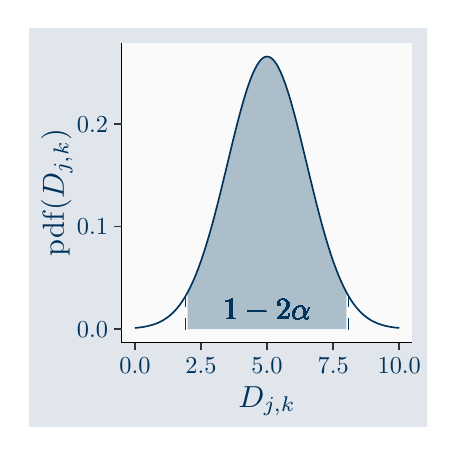
\begin{tikzpicture}[x=1pt,y=1pt]
\definecolor{fillColor}{RGB}{255,255,255}
\path[use as bounding box,fill=fillColor,fill opacity=0.00] (0,0) rectangle (144.54,144.54);
\begin{scope}
\path[clip] (  0.00,  0.00) rectangle (144.54,144.54);
\definecolor{drawColor}{RGB}{255,255,255}
\definecolor{fillColor}{RGB}{225,229,236}

\path[draw=drawColor,line width= 0.6pt,line join=round,line cap=round,fill=fillColor] (  0.00, -0.00) rectangle (144.54,144.54);
\end{scope}
\begin{scope}
\path[clip] ( 33.96, 30.72) rectangle (139.04,139.04);
\definecolor{fillColor}{gray}{0.98}

\path[fill=fillColor] ( 33.96, 30.72) rectangle (139.04,139.04);
\definecolor{fillColor}{RGB}{173,190,203}

\path[fill=fillColor] ( 57.84, 48.97) --
	( 58.80, 50.84) --
	( 59.75, 52.89) --
	( 60.71, 55.13) --
	( 61.66, 57.57) --
	( 62.62, 60.20) --
	( 63.57, 63.03) --
	( 64.53, 66.04) --
	( 65.49, 69.24) --
	( 66.44, 72.60) --
	( 67.40, 76.13) --
	( 68.35, 79.79) --
	( 69.31, 83.58) --
	( 70.26, 87.45) --
	( 71.22, 91.40) --
	( 72.17, 95.37) --
	( 73.13, 99.35) --
	( 74.08,103.29) --
	( 75.04,107.15) --
	( 75.99,110.90) --
	( 76.95,114.50) --
	( 77.90,117.90) --
	( 78.86,121.06) --
	( 79.81,123.96) --
	( 80.77,126.55) --
	( 81.72,128.80) --
	( 82.68,130.68) --
	( 83.64,132.17) --
	( 84.59,133.25) --
	( 85.55,133.90) --
	( 86.50,134.12) --
	( 87.46,133.90) --
	( 88.41,133.25) --
	( 89.37,132.17) --
	( 90.32,130.68) --
	( 91.28,128.80) --
	( 92.23,126.55) --
	( 93.19,123.96) --
	( 94.14,121.06) --
	( 95.10,117.90) --
	( 96.05,114.50) --
	( 97.01,110.90) --
	( 97.96,107.15) --
	( 98.92,103.29) --
	( 99.87, 99.35) --
	(100.83, 95.37) --
	(101.78, 91.40) --
	(102.74, 87.45) --
	(103.70, 83.58) --
	(104.65, 79.79) --
	(105.61, 76.13) --
	(106.56, 72.60) --
	(107.52, 69.24) --
	(108.47, 66.04) --
	(109.43, 63.03) --
	(110.38, 60.20) --
	(111.34, 57.57) --
	(112.29, 55.13) --
	(113.25, 52.89) --
	(114.20, 50.84) --
	(115.16, 48.97) --
	(115.16, 35.65) --
	(114.20, 35.65) --
	(113.25, 35.65) --
	(112.29, 35.65) --
	(111.34, 35.65) --
	(110.38, 35.65) --
	(109.43, 35.65) --
	(108.47, 35.65) --
	(107.52, 35.65) --
	(106.56, 35.65) --
	(105.61, 35.65) --
	(104.65, 35.65) --
	(103.70, 35.65) --
	(102.74, 35.65) --
	(101.78, 35.65) --
	(100.83, 35.65) --
	( 99.87, 35.65) --
	( 98.92, 35.65) --
	( 97.96, 35.65) --
	( 97.01, 35.65) --
	( 96.05, 35.65) --
	( 95.10, 35.65) --
	( 94.14, 35.65) --
	( 93.19, 35.65) --
	( 92.23, 35.65) --
	( 91.28, 35.65) --
	( 90.32, 35.65) --
	( 89.37, 35.65) --
	( 88.41, 35.65) --
	( 87.46, 35.65) --
	( 86.50, 35.65) --
	( 85.55, 35.65) --
	( 84.59, 35.65) --
	( 83.64, 35.65) --
	( 82.68, 35.65) --
	( 81.72, 35.65) --
	( 80.77, 35.65) --
	( 79.81, 35.65) --
	( 78.86, 35.65) --
	( 77.90, 35.65) --
	( 76.95, 35.65) --
	( 75.99, 35.65) --
	( 75.04, 35.65) --
	( 74.08, 35.65) --
	( 73.13, 35.65) --
	( 72.17, 35.65) --
	( 71.22, 35.65) --
	( 70.26, 35.65) --
	( 69.31, 35.65) --
	( 68.35, 35.65) --
	( 67.40, 35.65) --
	( 66.44, 35.65) --
	( 65.49, 35.65) --
	( 64.53, 35.65) --
	( 63.57, 35.65) --
	( 62.62, 35.65) --
	( 61.66, 35.65) --
	( 60.71, 35.65) --
	( 59.75, 35.65) --
	( 58.80, 35.65) --
	( 57.84, 35.65) --
	cycle;
\definecolor{drawColor}{RGB}{0,52,92}

\path[draw=drawColor,line width= 0.6pt,line join=round] ( 38.74, 36.03) --
	( 39.69, 36.12) --
	( 40.65, 36.24) --
	( 41.60, 36.37) --
	( 42.56, 36.54) --
	( 43.51, 36.74) --
	( 44.47, 36.98) --
	( 45.42, 37.27) --
	( 46.38, 37.60) --
	( 47.34, 38.00) --
	( 48.29, 38.46) --
	( 49.25, 39.00) --
	( 50.20, 39.63) --
	( 51.16, 40.35) --
	( 52.11, 41.18) --
	( 53.07, 42.12) --
	( 54.02, 43.19) --
	( 54.98, 44.40) --
	( 55.93, 45.76) --
	( 56.89, 47.29) --
	( 57.84, 48.97) --
	( 58.80, 50.84) --
	( 59.75, 52.89) --
	( 60.71, 55.13) --
	( 61.66, 57.57) --
	( 62.62, 60.20) --
	( 63.57, 63.03) --
	( 64.53, 66.04) --
	( 65.49, 69.24) --
	( 66.44, 72.60) --
	( 67.40, 76.13) --
	( 68.35, 79.79) --
	( 69.31, 83.58) --
	( 70.26, 87.45) --
	( 71.22, 91.40) --
	( 72.17, 95.37) --
	( 73.13, 99.35) --
	( 74.08,103.29) --
	( 75.04,107.15) --
	( 75.99,110.90) --
	( 76.95,114.50) --
	( 77.90,117.90) --
	( 78.86,121.06) --
	( 79.81,123.96) --
	( 80.77,126.55) --
	( 81.72,128.80) --
	( 82.68,130.68) --
	( 83.64,132.17) --
	( 84.59,133.25) --
	( 85.55,133.90) --
	( 86.50,134.12) --
	( 87.46,133.90) --
	( 88.41,133.25) --
	( 89.37,132.17) --
	( 90.32,130.68) --
	( 91.28,128.80) --
	( 92.23,126.55) --
	( 93.19,123.96) --
	( 94.14,121.06) --
	( 95.10,117.90) --
	( 96.05,114.50) --
	( 97.01,110.90) --
	( 97.96,107.15) --
	( 98.92,103.29) --
	( 99.87, 99.35) --
	(100.83, 95.37) --
	(101.78, 91.40) --
	(102.74, 87.45) --
	(103.70, 83.58) --
	(104.65, 79.79) --
	(105.61, 76.13) --
	(106.56, 72.60) --
	(107.52, 69.24) --
	(108.47, 66.04) --
	(109.43, 63.03) --
	(110.38, 60.20) --
	(111.34, 57.57) --
	(112.29, 55.13) --
	(113.25, 52.89) --
	(114.20, 50.84) --
	(115.16, 48.97) --
	(116.11, 47.29) --
	(117.07, 45.76) --
	(118.02, 44.40) --
	(118.98, 43.19) --
	(119.93, 42.12) --
	(120.89, 41.18) --
	(121.85, 40.35) --
	(122.80, 39.63) --
	(123.76, 39.00) --
	(124.71, 38.46) --
	(125.67, 38.00) --
	(126.62, 37.60) --
	(127.58, 37.27) --
	(128.53, 36.98) --
	(129.49, 36.74) --
	(130.44, 36.54) --
	(131.40, 36.37) --
	(132.35, 36.24) --
	(133.31, 36.12) --
	(134.26, 36.03);

\path[draw=drawColor,line width= 0.6pt,dash pattern=on 4pt off 4pt ,line join=round] ( 57.07, 35.65) -- ( 57.07, 47.60);

\path[draw=drawColor,line width= 0.6pt,dash pattern=on 4pt off 4pt ,line join=round] ( 57.07, 35.65) -- ( 57.07, 47.60);

\path[draw=drawColor,line width= 0.6pt,dash pattern=on 4pt off 4pt ,line join=round] ( 57.07, 35.65) -- ( 57.07, 47.60);

\path[draw=drawColor,line width= 0.6pt,dash pattern=on 4pt off 4pt ,line join=round] ( 57.07, 35.65) -- ( 57.07, 47.60);

\path[draw=drawColor,line width= 0.6pt,dash pattern=on 4pt off 4pt ,line join=round] ( 57.07, 35.65) -- ( 57.07, 47.60);

\path[draw=drawColor,line width= 0.6pt,dash pattern=on 4pt off 4pt ,line join=round] ( 57.07, 35.65) -- ( 57.07, 47.60);

\path[draw=drawColor,line width= 0.6pt,dash pattern=on 4pt off 4pt ,line join=round] ( 57.07, 35.65) -- ( 57.07, 47.60);

\path[draw=drawColor,line width= 0.6pt,dash pattern=on 4pt off 4pt ,line join=round] ( 57.07, 35.65) -- ( 57.07, 47.60);

\path[draw=drawColor,line width= 0.6pt,dash pattern=on 4pt off 4pt ,line join=round] ( 57.07, 35.65) -- ( 57.07, 47.60);

\path[draw=drawColor,line width= 0.6pt,dash pattern=on 4pt off 4pt ,line join=round] ( 57.07, 35.65) -- ( 57.07, 47.60);

\path[draw=drawColor,line width= 0.6pt,dash pattern=on 4pt off 4pt ,line join=round] ( 57.07, 35.65) -- ( 57.07, 47.60);

\path[draw=drawColor,line width= 0.6pt,dash pattern=on 4pt off 4pt ,line join=round] ( 57.07, 35.65) -- ( 57.07, 47.60);

\path[draw=drawColor,line width= 0.6pt,dash pattern=on 4pt off 4pt ,line join=round] ( 57.07, 35.65) -- ( 57.07, 47.60);

\path[draw=drawColor,line width= 0.6pt,dash pattern=on 4pt off 4pt ,line join=round] ( 57.07, 35.65) -- ( 57.07, 47.60);

\path[draw=drawColor,line width= 0.6pt,dash pattern=on 4pt off 4pt ,line join=round] ( 57.07, 35.65) -- ( 57.07, 47.60);

\path[draw=drawColor,line width= 0.6pt,dash pattern=on 4pt off 4pt ,line join=round] ( 57.07, 35.65) -- ( 57.07, 47.60);

\path[draw=drawColor,line width= 0.6pt,dash pattern=on 4pt off 4pt ,line join=round] ( 57.07, 35.65) -- ( 57.07, 47.60);

\path[draw=drawColor,line width= 0.6pt,dash pattern=on 4pt off 4pt ,line join=round] ( 57.07, 35.65) -- ( 57.07, 47.60);

\path[draw=drawColor,line width= 0.6pt,dash pattern=on 4pt off 4pt ,line join=round] ( 57.07, 35.65) -- ( 57.07, 47.60);

\path[draw=drawColor,line width= 0.6pt,dash pattern=on 4pt off 4pt ,line join=round] ( 57.07, 35.65) -- ( 57.07, 47.60);

\path[draw=drawColor,line width= 0.6pt,dash pattern=on 4pt off 4pt ,line join=round] ( 57.07, 35.65) -- ( 57.07, 47.60);

\path[draw=drawColor,line width= 0.6pt,dash pattern=on 4pt off 4pt ,line join=round] ( 57.07, 35.65) -- ( 57.07, 47.60);

\path[draw=drawColor,line width= 0.6pt,dash pattern=on 4pt off 4pt ,line join=round] ( 57.07, 35.65) -- ( 57.07, 47.60);

\path[draw=drawColor,line width= 0.6pt,dash pattern=on 4pt off 4pt ,line join=round] ( 57.07, 35.65) -- ( 57.07, 47.60);

\path[draw=drawColor,line width= 0.6pt,dash pattern=on 4pt off 4pt ,line join=round] ( 57.07, 35.65) -- ( 57.07, 47.60);

\path[draw=drawColor,line width= 0.6pt,dash pattern=on 4pt off 4pt ,line join=round] ( 57.07, 35.65) -- ( 57.07, 47.60);

\path[draw=drawColor,line width= 0.6pt,dash pattern=on 4pt off 4pt ,line join=round] ( 57.07, 35.65) -- ( 57.07, 47.60);

\path[draw=drawColor,line width= 0.6pt,dash pattern=on 4pt off 4pt ,line join=round] ( 57.07, 35.65) -- ( 57.07, 47.60);

\path[draw=drawColor,line width= 0.6pt,dash pattern=on 4pt off 4pt ,line join=round] ( 57.07, 35.65) -- ( 57.07, 47.60);

\path[draw=drawColor,line width= 0.6pt,dash pattern=on 4pt off 4pt ,line join=round] ( 57.07, 35.65) -- ( 57.07, 47.60);

\path[draw=drawColor,line width= 0.6pt,dash pattern=on 4pt off 4pt ,line join=round] ( 57.07, 35.65) -- ( 57.07, 47.60);

\path[draw=drawColor,line width= 0.6pt,dash pattern=on 4pt off 4pt ,line join=round] ( 57.07, 35.65) -- ( 57.07, 47.60);

\path[draw=drawColor,line width= 0.6pt,dash pattern=on 4pt off 4pt ,line join=round] ( 57.07, 35.65) -- ( 57.07, 47.60);

\path[draw=drawColor,line width= 0.6pt,dash pattern=on 4pt off 4pt ,line join=round] ( 57.07, 35.65) -- ( 57.07, 47.60);

\path[draw=drawColor,line width= 0.6pt,dash pattern=on 4pt off 4pt ,line join=round] ( 57.07, 35.65) -- ( 57.07, 47.60);

\path[draw=drawColor,line width= 0.6pt,dash pattern=on 4pt off 4pt ,line join=round] ( 57.07, 35.65) -- ( 57.07, 47.60);

\path[draw=drawColor,line width= 0.6pt,dash pattern=on 4pt off 4pt ,line join=round] ( 57.07, 35.65) -- ( 57.07, 47.60);

\path[draw=drawColor,line width= 0.6pt,dash pattern=on 4pt off 4pt ,line join=round] ( 57.07, 35.65) -- ( 57.07, 47.60);

\path[draw=drawColor,line width= 0.6pt,dash pattern=on 4pt off 4pt ,line join=round] ( 57.07, 35.65) -- ( 57.07, 47.60);

\path[draw=drawColor,line width= 0.6pt,dash pattern=on 4pt off 4pt ,line join=round] ( 57.07, 35.65) -- ( 57.07, 47.60);

\path[draw=drawColor,line width= 0.6pt,dash pattern=on 4pt off 4pt ,line join=round] ( 57.07, 35.65) -- ( 57.07, 47.60);

\path[draw=drawColor,line width= 0.6pt,dash pattern=on 4pt off 4pt ,line join=round] ( 57.07, 35.65) -- ( 57.07, 47.60);

\path[draw=drawColor,line width= 0.6pt,dash pattern=on 4pt off 4pt ,line join=round] ( 57.07, 35.65) -- ( 57.07, 47.60);

\path[draw=drawColor,line width= 0.6pt,dash pattern=on 4pt off 4pt ,line join=round] ( 57.07, 35.65) -- ( 57.07, 47.60);

\path[draw=drawColor,line width= 0.6pt,dash pattern=on 4pt off 4pt ,line join=round] ( 57.07, 35.65) -- ( 57.07, 47.60);

\path[draw=drawColor,line width= 0.6pt,dash pattern=on 4pt off 4pt ,line join=round] ( 57.07, 35.65) -- ( 57.07, 47.60);

\path[draw=drawColor,line width= 0.6pt,dash pattern=on 4pt off 4pt ,line join=round] ( 57.07, 35.65) -- ( 57.07, 47.60);

\path[draw=drawColor,line width= 0.6pt,dash pattern=on 4pt off 4pt ,line join=round] ( 57.07, 35.65) -- ( 57.07, 47.60);

\path[draw=drawColor,line width= 0.6pt,dash pattern=on 4pt off 4pt ,line join=round] ( 57.07, 35.65) -- ( 57.07, 47.60);

\path[draw=drawColor,line width= 0.6pt,dash pattern=on 4pt off 4pt ,line join=round] ( 57.07, 35.65) -- ( 57.07, 47.60);

\path[draw=drawColor,line width= 0.6pt,dash pattern=on 4pt off 4pt ,line join=round] ( 57.07, 35.65) -- ( 57.07, 47.60);

\path[draw=drawColor,line width= 0.6pt,dash pattern=on 4pt off 4pt ,line join=round] ( 57.07, 35.65) -- ( 57.07, 47.60);

\path[draw=drawColor,line width= 0.6pt,dash pattern=on 4pt off 4pt ,line join=round] ( 57.07, 35.65) -- ( 57.07, 47.60);

\path[draw=drawColor,line width= 0.6pt,dash pattern=on 4pt off 4pt ,line join=round] ( 57.07, 35.65) -- ( 57.07, 47.60);

\path[draw=drawColor,line width= 0.6pt,dash pattern=on 4pt off 4pt ,line join=round] ( 57.07, 35.65) -- ( 57.07, 47.60);

\path[draw=drawColor,line width= 0.6pt,dash pattern=on 4pt off 4pt ,line join=round] ( 57.07, 35.65) -- ( 57.07, 47.60);

\path[draw=drawColor,line width= 0.6pt,dash pattern=on 4pt off 4pt ,line join=round] ( 57.07, 35.65) -- ( 57.07, 47.60);

\path[draw=drawColor,line width= 0.6pt,dash pattern=on 4pt off 4pt ,line join=round] ( 57.07, 35.65) -- ( 57.07, 47.60);

\path[draw=drawColor,line width= 0.6pt,dash pattern=on 4pt off 4pt ,line join=round] ( 57.07, 35.65) -- ( 57.07, 47.60);

\path[draw=drawColor,line width= 0.6pt,dash pattern=on 4pt off 4pt ,line join=round] ( 57.07, 35.65) -- ( 57.07, 47.60);

\path[draw=drawColor,line width= 0.6pt,dash pattern=on 4pt off 4pt ,line join=round] ( 57.07, 35.65) -- ( 57.07, 47.60);

\path[draw=drawColor,line width= 0.6pt,dash pattern=on 4pt off 4pt ,line join=round] ( 57.07, 35.65) -- ( 57.07, 47.60);

\path[draw=drawColor,line width= 0.6pt,dash pattern=on 4pt off 4pt ,line join=round] ( 57.07, 35.65) -- ( 57.07, 47.60);

\path[draw=drawColor,line width= 0.6pt,dash pattern=on 4pt off 4pt ,line join=round] ( 57.07, 35.65) -- ( 57.07, 47.60);

\path[draw=drawColor,line width= 0.6pt,dash pattern=on 4pt off 4pt ,line join=round] ( 57.07, 35.65) -- ( 57.07, 47.60);

\path[draw=drawColor,line width= 0.6pt,dash pattern=on 4pt off 4pt ,line join=round] ( 57.07, 35.65) -- ( 57.07, 47.60);

\path[draw=drawColor,line width= 0.6pt,dash pattern=on 4pt off 4pt ,line join=round] ( 57.07, 35.65) -- ( 57.07, 47.60);

\path[draw=drawColor,line width= 0.6pt,dash pattern=on 4pt off 4pt ,line join=round] ( 57.07, 35.65) -- ( 57.07, 47.60);

\path[draw=drawColor,line width= 0.6pt,dash pattern=on 4pt off 4pt ,line join=round] ( 57.07, 35.65) -- ( 57.07, 47.60);

\path[draw=drawColor,line width= 0.6pt,dash pattern=on 4pt off 4pt ,line join=round] ( 57.07, 35.65) -- ( 57.07, 47.60);

\path[draw=drawColor,line width= 0.6pt,dash pattern=on 4pt off 4pt ,line join=round] ( 57.07, 35.65) -- ( 57.07, 47.60);

\path[draw=drawColor,line width= 0.6pt,dash pattern=on 4pt off 4pt ,line join=round] ( 57.07, 35.65) -- ( 57.07, 47.60);

\path[draw=drawColor,line width= 0.6pt,dash pattern=on 4pt off 4pt ,line join=round] ( 57.07, 35.65) -- ( 57.07, 47.60);

\path[draw=drawColor,line width= 0.6pt,dash pattern=on 4pt off 4pt ,line join=round] ( 57.07, 35.65) -- ( 57.07, 47.60);

\path[draw=drawColor,line width= 0.6pt,dash pattern=on 4pt off 4pt ,line join=round] ( 57.07, 35.65) -- ( 57.07, 47.60);

\path[draw=drawColor,line width= 0.6pt,dash pattern=on 4pt off 4pt ,line join=round] ( 57.07, 35.65) -- ( 57.07, 47.60);

\path[draw=drawColor,line width= 0.6pt,dash pattern=on 4pt off 4pt ,line join=round] ( 57.07, 35.65) -- ( 57.07, 47.60);

\path[draw=drawColor,line width= 0.6pt,dash pattern=on 4pt off 4pt ,line join=round] ( 57.07, 35.65) -- ( 57.07, 47.60);

\path[draw=drawColor,line width= 0.6pt,dash pattern=on 4pt off 4pt ,line join=round] ( 57.07, 35.65) -- ( 57.07, 47.60);

\path[draw=drawColor,line width= 0.6pt,dash pattern=on 4pt off 4pt ,line join=round] ( 57.07, 35.65) -- ( 57.07, 47.60);

\path[draw=drawColor,line width= 0.6pt,dash pattern=on 4pt off 4pt ,line join=round] ( 57.07, 35.65) -- ( 57.07, 47.60);

\path[draw=drawColor,line width= 0.6pt,dash pattern=on 4pt off 4pt ,line join=round] ( 57.07, 35.65) -- ( 57.07, 47.60);

\path[draw=drawColor,line width= 0.6pt,dash pattern=on 4pt off 4pt ,line join=round] ( 57.07, 35.65) -- ( 57.07, 47.60);

\path[draw=drawColor,line width= 0.6pt,dash pattern=on 4pt off 4pt ,line join=round] ( 57.07, 35.65) -- ( 57.07, 47.60);

\path[draw=drawColor,line width= 0.6pt,dash pattern=on 4pt off 4pt ,line join=round] ( 57.07, 35.65) -- ( 57.07, 47.60);

\path[draw=drawColor,line width= 0.6pt,dash pattern=on 4pt off 4pt ,line join=round] ( 57.07, 35.65) -- ( 57.07, 47.60);

\path[draw=drawColor,line width= 0.6pt,dash pattern=on 4pt off 4pt ,line join=round] ( 57.07, 35.65) -- ( 57.07, 47.60);

\path[draw=drawColor,line width= 0.6pt,dash pattern=on 4pt off 4pt ,line join=round] ( 57.07, 35.65) -- ( 57.07, 47.60);

\path[draw=drawColor,line width= 0.6pt,dash pattern=on 4pt off 4pt ,line join=round] ( 57.07, 35.65) -- ( 57.07, 47.60);

\path[draw=drawColor,line width= 0.6pt,dash pattern=on 4pt off 4pt ,line join=round] ( 57.07, 35.65) -- ( 57.07, 47.60);

\path[draw=drawColor,line width= 0.6pt,dash pattern=on 4pt off 4pt ,line join=round] ( 57.07, 35.65) -- ( 57.07, 47.60);

\path[draw=drawColor,line width= 0.6pt,dash pattern=on 4pt off 4pt ,line join=round] ( 57.07, 35.65) -- ( 57.07, 47.60);

\path[draw=drawColor,line width= 0.6pt,dash pattern=on 4pt off 4pt ,line join=round] ( 57.07, 35.65) -- ( 57.07, 47.60);

\path[draw=drawColor,line width= 0.6pt,dash pattern=on 4pt off 4pt ,line join=round] ( 57.07, 35.65) -- ( 57.07, 47.60);

\path[draw=drawColor,line width= 0.6pt,dash pattern=on 4pt off 4pt ,line join=round] ( 57.07, 35.65) -- ( 57.07, 47.60);

\path[draw=drawColor,line width= 0.6pt,dash pattern=on 4pt off 4pt ,line join=round] ( 57.07, 35.65) -- ( 57.07, 47.60);

\path[draw=drawColor,line width= 0.6pt,dash pattern=on 4pt off 4pt ,line join=round] ( 57.07, 35.65) -- ( 57.07, 47.60);

\path[draw=drawColor,line width= 0.6pt,dash pattern=on 4pt off 4pt ,line join=round] ( 57.07, 35.65) -- ( 57.07, 47.60);

\path[draw=drawColor,line width= 0.6pt,dash pattern=on 4pt off 4pt ,line join=round] ( 57.07, 35.65) -- ( 57.07, 47.60);

\path[draw=drawColor,line width= 0.6pt,dash pattern=on 4pt off 4pt ,line join=round] ( 57.07, 35.65) -- ( 57.07, 47.60);

\path[draw=drawColor,line width= 0.6pt,dash pattern=on 4pt off 4pt ,line join=round] ( 57.07, 35.65) -- ( 57.07, 47.60);

\path[draw=drawColor,line width= 0.6pt,dash pattern=on 4pt off 4pt ,line join=round] (115.93, 35.65) -- (115.93, 47.60);

\path[draw=drawColor,line width= 0.6pt,dash pattern=on 4pt off 4pt ,line join=round] (115.93, 35.65) -- (115.93, 47.60);

\path[draw=drawColor,line width= 0.6pt,dash pattern=on 4pt off 4pt ,line join=round] (115.93, 35.65) -- (115.93, 47.60);

\path[draw=drawColor,line width= 0.6pt,dash pattern=on 4pt off 4pt ,line join=round] (115.93, 35.65) -- (115.93, 47.60);

\path[draw=drawColor,line width= 0.6pt,dash pattern=on 4pt off 4pt ,line join=round] (115.93, 35.65) -- (115.93, 47.60);

\path[draw=drawColor,line width= 0.6pt,dash pattern=on 4pt off 4pt ,line join=round] (115.93, 35.65) -- (115.93, 47.60);

\path[draw=drawColor,line width= 0.6pt,dash pattern=on 4pt off 4pt ,line join=round] (115.93, 35.65) -- (115.93, 47.60);

\path[draw=drawColor,line width= 0.6pt,dash pattern=on 4pt off 4pt ,line join=round] (115.93, 35.65) -- (115.93, 47.60);

\path[draw=drawColor,line width= 0.6pt,dash pattern=on 4pt off 4pt ,line join=round] (115.93, 35.65) -- (115.93, 47.60);

\path[draw=drawColor,line width= 0.6pt,dash pattern=on 4pt off 4pt ,line join=round] (115.93, 35.65) -- (115.93, 47.60);

\path[draw=drawColor,line width= 0.6pt,dash pattern=on 4pt off 4pt ,line join=round] (115.93, 35.65) -- (115.93, 47.60);

\path[draw=drawColor,line width= 0.6pt,dash pattern=on 4pt off 4pt ,line join=round] (115.93, 35.65) -- (115.93, 47.60);

\path[draw=drawColor,line width= 0.6pt,dash pattern=on 4pt off 4pt ,line join=round] (115.93, 35.65) -- (115.93, 47.60);

\path[draw=drawColor,line width= 0.6pt,dash pattern=on 4pt off 4pt ,line join=round] (115.93, 35.65) -- (115.93, 47.60);

\path[draw=drawColor,line width= 0.6pt,dash pattern=on 4pt off 4pt ,line join=round] (115.93, 35.65) -- (115.93, 47.60);

\path[draw=drawColor,line width= 0.6pt,dash pattern=on 4pt off 4pt ,line join=round] (115.93, 35.65) -- (115.93, 47.60);

\path[draw=drawColor,line width= 0.6pt,dash pattern=on 4pt off 4pt ,line join=round] (115.93, 35.65) -- (115.93, 47.60);

\path[draw=drawColor,line width= 0.6pt,dash pattern=on 4pt off 4pt ,line join=round] (115.93, 35.65) -- (115.93, 47.60);

\path[draw=drawColor,line width= 0.6pt,dash pattern=on 4pt off 4pt ,line join=round] (115.93, 35.65) -- (115.93, 47.60);

\path[draw=drawColor,line width= 0.6pt,dash pattern=on 4pt off 4pt ,line join=round] (115.93, 35.65) -- (115.93, 47.60);

\path[draw=drawColor,line width= 0.6pt,dash pattern=on 4pt off 4pt ,line join=round] (115.93, 35.65) -- (115.93, 47.60);

\path[draw=drawColor,line width= 0.6pt,dash pattern=on 4pt off 4pt ,line join=round] (115.93, 35.65) -- (115.93, 47.60);

\path[draw=drawColor,line width= 0.6pt,dash pattern=on 4pt off 4pt ,line join=round] (115.93, 35.65) -- (115.93, 47.60);

\path[draw=drawColor,line width= 0.6pt,dash pattern=on 4pt off 4pt ,line join=round] (115.93, 35.65) -- (115.93, 47.60);

\path[draw=drawColor,line width= 0.6pt,dash pattern=on 4pt off 4pt ,line join=round] (115.93, 35.65) -- (115.93, 47.60);

\path[draw=drawColor,line width= 0.6pt,dash pattern=on 4pt off 4pt ,line join=round] (115.93, 35.65) -- (115.93, 47.60);

\path[draw=drawColor,line width= 0.6pt,dash pattern=on 4pt off 4pt ,line join=round] (115.93, 35.65) -- (115.93, 47.60);

\path[draw=drawColor,line width= 0.6pt,dash pattern=on 4pt off 4pt ,line join=round] (115.93, 35.65) -- (115.93, 47.60);

\path[draw=drawColor,line width= 0.6pt,dash pattern=on 4pt off 4pt ,line join=round] (115.93, 35.65) -- (115.93, 47.60);

\path[draw=drawColor,line width= 0.6pt,dash pattern=on 4pt off 4pt ,line join=round] (115.93, 35.65) -- (115.93, 47.60);

\path[draw=drawColor,line width= 0.6pt,dash pattern=on 4pt off 4pt ,line join=round] (115.93, 35.65) -- (115.93, 47.60);

\path[draw=drawColor,line width= 0.6pt,dash pattern=on 4pt off 4pt ,line join=round] (115.93, 35.65) -- (115.93, 47.60);

\path[draw=drawColor,line width= 0.6pt,dash pattern=on 4pt off 4pt ,line join=round] (115.93, 35.65) -- (115.93, 47.60);

\path[draw=drawColor,line width= 0.6pt,dash pattern=on 4pt off 4pt ,line join=round] (115.93, 35.65) -- (115.93, 47.60);

\path[draw=drawColor,line width= 0.6pt,dash pattern=on 4pt off 4pt ,line join=round] (115.93, 35.65) -- (115.93, 47.60);

\path[draw=drawColor,line width= 0.6pt,dash pattern=on 4pt off 4pt ,line join=round] (115.93, 35.65) -- (115.93, 47.60);

\path[draw=drawColor,line width= 0.6pt,dash pattern=on 4pt off 4pt ,line join=round] (115.93, 35.65) -- (115.93, 47.60);

\path[draw=drawColor,line width= 0.6pt,dash pattern=on 4pt off 4pt ,line join=round] (115.93, 35.65) -- (115.93, 47.60);

\path[draw=drawColor,line width= 0.6pt,dash pattern=on 4pt off 4pt ,line join=round] (115.93, 35.65) -- (115.93, 47.60);

\path[draw=drawColor,line width= 0.6pt,dash pattern=on 4pt off 4pt ,line join=round] (115.93, 35.65) -- (115.93, 47.60);

\path[draw=drawColor,line width= 0.6pt,dash pattern=on 4pt off 4pt ,line join=round] (115.93, 35.65) -- (115.93, 47.60);

\path[draw=drawColor,line width= 0.6pt,dash pattern=on 4pt off 4pt ,line join=round] (115.93, 35.65) -- (115.93, 47.60);

\path[draw=drawColor,line width= 0.6pt,dash pattern=on 4pt off 4pt ,line join=round] (115.93, 35.65) -- (115.93, 47.60);

\path[draw=drawColor,line width= 0.6pt,dash pattern=on 4pt off 4pt ,line join=round] (115.93, 35.65) -- (115.93, 47.60);

\path[draw=drawColor,line width= 0.6pt,dash pattern=on 4pt off 4pt ,line join=round] (115.93, 35.65) -- (115.93, 47.60);

\path[draw=drawColor,line width= 0.6pt,dash pattern=on 4pt off 4pt ,line join=round] (115.93, 35.65) -- (115.93, 47.60);

\path[draw=drawColor,line width= 0.6pt,dash pattern=on 4pt off 4pt ,line join=round] (115.93, 35.65) -- (115.93, 47.60);

\path[draw=drawColor,line width= 0.6pt,dash pattern=on 4pt off 4pt ,line join=round] (115.93, 35.65) -- (115.93, 47.60);

\path[draw=drawColor,line width= 0.6pt,dash pattern=on 4pt off 4pt ,line join=round] (115.93, 35.65) -- (115.93, 47.60);

\path[draw=drawColor,line width= 0.6pt,dash pattern=on 4pt off 4pt ,line join=round] (115.93, 35.65) -- (115.93, 47.60);

\path[draw=drawColor,line width= 0.6pt,dash pattern=on 4pt off 4pt ,line join=round] (115.93, 35.65) -- (115.93, 47.60);

\path[draw=drawColor,line width= 0.6pt,dash pattern=on 4pt off 4pt ,line join=round] (115.93, 35.65) -- (115.93, 47.60);

\path[draw=drawColor,line width= 0.6pt,dash pattern=on 4pt off 4pt ,line join=round] (115.93, 35.65) -- (115.93, 47.60);

\path[draw=drawColor,line width= 0.6pt,dash pattern=on 4pt off 4pt ,line join=round] (115.93, 35.65) -- (115.93, 47.60);

\path[draw=drawColor,line width= 0.6pt,dash pattern=on 4pt off 4pt ,line join=round] (115.93, 35.65) -- (115.93, 47.60);

\path[draw=drawColor,line width= 0.6pt,dash pattern=on 4pt off 4pt ,line join=round] (115.93, 35.65) -- (115.93, 47.60);

\path[draw=drawColor,line width= 0.6pt,dash pattern=on 4pt off 4pt ,line join=round] (115.93, 35.65) -- (115.93, 47.60);

\path[draw=drawColor,line width= 0.6pt,dash pattern=on 4pt off 4pt ,line join=round] (115.93, 35.65) -- (115.93, 47.60);

\path[draw=drawColor,line width= 0.6pt,dash pattern=on 4pt off 4pt ,line join=round] (115.93, 35.65) -- (115.93, 47.60);

\path[draw=drawColor,line width= 0.6pt,dash pattern=on 4pt off 4pt ,line join=round] (115.93, 35.65) -- (115.93, 47.60);

\path[draw=drawColor,line width= 0.6pt,dash pattern=on 4pt off 4pt ,line join=round] (115.93, 35.65) -- (115.93, 47.60);

\path[draw=drawColor,line width= 0.6pt,dash pattern=on 4pt off 4pt ,line join=round] (115.93, 35.65) -- (115.93, 47.60);

\path[draw=drawColor,line width= 0.6pt,dash pattern=on 4pt off 4pt ,line join=round] (115.93, 35.65) -- (115.93, 47.60);

\path[draw=drawColor,line width= 0.6pt,dash pattern=on 4pt off 4pt ,line join=round] (115.93, 35.65) -- (115.93, 47.60);

\path[draw=drawColor,line width= 0.6pt,dash pattern=on 4pt off 4pt ,line join=round] (115.93, 35.65) -- (115.93, 47.60);

\path[draw=drawColor,line width= 0.6pt,dash pattern=on 4pt off 4pt ,line join=round] (115.93, 35.65) -- (115.93, 47.60);

\path[draw=drawColor,line width= 0.6pt,dash pattern=on 4pt off 4pt ,line join=round] (115.93, 35.65) -- (115.93, 47.60);

\path[draw=drawColor,line width= 0.6pt,dash pattern=on 4pt off 4pt ,line join=round] (115.93, 35.65) -- (115.93, 47.60);

\path[draw=drawColor,line width= 0.6pt,dash pattern=on 4pt off 4pt ,line join=round] (115.93, 35.65) -- (115.93, 47.60);

\path[draw=drawColor,line width= 0.6pt,dash pattern=on 4pt off 4pt ,line join=round] (115.93, 35.65) -- (115.93, 47.60);

\path[draw=drawColor,line width= 0.6pt,dash pattern=on 4pt off 4pt ,line join=round] (115.93, 35.65) -- (115.93, 47.60);

\path[draw=drawColor,line width= 0.6pt,dash pattern=on 4pt off 4pt ,line join=round] (115.93, 35.65) -- (115.93, 47.60);

\path[draw=drawColor,line width= 0.6pt,dash pattern=on 4pt off 4pt ,line join=round] (115.93, 35.65) -- (115.93, 47.60);

\path[draw=drawColor,line width= 0.6pt,dash pattern=on 4pt off 4pt ,line join=round] (115.93, 35.65) -- (115.93, 47.60);

\path[draw=drawColor,line width= 0.6pt,dash pattern=on 4pt off 4pt ,line join=round] (115.93, 35.65) -- (115.93, 47.60);

\path[draw=drawColor,line width= 0.6pt,dash pattern=on 4pt off 4pt ,line join=round] (115.93, 35.65) -- (115.93, 47.60);

\path[draw=drawColor,line width= 0.6pt,dash pattern=on 4pt off 4pt ,line join=round] (115.93, 35.65) -- (115.93, 47.60);

\path[draw=drawColor,line width= 0.6pt,dash pattern=on 4pt off 4pt ,line join=round] (115.93, 35.65) -- (115.93, 47.60);

\path[draw=drawColor,line width= 0.6pt,dash pattern=on 4pt off 4pt ,line join=round] (115.93, 35.65) -- (115.93, 47.60);

\path[draw=drawColor,line width= 0.6pt,dash pattern=on 4pt off 4pt ,line join=round] (115.93, 35.65) -- (115.93, 47.60);

\path[draw=drawColor,line width= 0.6pt,dash pattern=on 4pt off 4pt ,line join=round] (115.93, 35.65) -- (115.93, 47.60);

\path[draw=drawColor,line width= 0.6pt,dash pattern=on 4pt off 4pt ,line join=round] (115.93, 35.65) -- (115.93, 47.60);

\path[draw=drawColor,line width= 0.6pt,dash pattern=on 4pt off 4pt ,line join=round] (115.93, 35.65) -- (115.93, 47.60);

\path[draw=drawColor,line width= 0.6pt,dash pattern=on 4pt off 4pt ,line join=round] (115.93, 35.65) -- (115.93, 47.60);

\path[draw=drawColor,line width= 0.6pt,dash pattern=on 4pt off 4pt ,line join=round] (115.93, 35.65) -- (115.93, 47.60);

\path[draw=drawColor,line width= 0.6pt,dash pattern=on 4pt off 4pt ,line join=round] (115.93, 35.65) -- (115.93, 47.60);

\path[draw=drawColor,line width= 0.6pt,dash pattern=on 4pt off 4pt ,line join=round] (115.93, 35.65) -- (115.93, 47.60);

\path[draw=drawColor,line width= 0.6pt,dash pattern=on 4pt off 4pt ,line join=round] (115.93, 35.65) -- (115.93, 47.60);

\path[draw=drawColor,line width= 0.6pt,dash pattern=on 4pt off 4pt ,line join=round] (115.93, 35.65) -- (115.93, 47.60);

\path[draw=drawColor,line width= 0.6pt,dash pattern=on 4pt off 4pt ,line join=round] (115.93, 35.65) -- (115.93, 47.60);

\path[draw=drawColor,line width= 0.6pt,dash pattern=on 4pt off 4pt ,line join=round] (115.93, 35.65) -- (115.93, 47.60);

\path[draw=drawColor,line width= 0.6pt,dash pattern=on 4pt off 4pt ,line join=round] (115.93, 35.65) -- (115.93, 47.60);

\path[draw=drawColor,line width= 0.6pt,dash pattern=on 4pt off 4pt ,line join=round] (115.93, 35.65) -- (115.93, 47.60);

\path[draw=drawColor,line width= 0.6pt,dash pattern=on 4pt off 4pt ,line join=round] (115.93, 35.65) -- (115.93, 47.60);

\path[draw=drawColor,line width= 0.6pt,dash pattern=on 4pt off 4pt ,line join=round] (115.93, 35.65) -- (115.93, 47.60);

\path[draw=drawColor,line width= 0.6pt,dash pattern=on 4pt off 4pt ,line join=round] (115.93, 35.65) -- (115.93, 47.60);

\path[draw=drawColor,line width= 0.6pt,dash pattern=on 4pt off 4pt ,line join=round] (115.93, 35.65) -- (115.93, 47.60);

\path[draw=drawColor,line width= 0.6pt,dash pattern=on 4pt off 4pt ,line join=round] (115.93, 35.65) -- (115.93, 47.60);

\path[draw=drawColor,line width= 0.6pt,dash pattern=on 4pt off 4pt ,line join=round] (115.93, 35.65) -- (115.93, 47.60);

\path[draw=drawColor,line width= 0.6pt,dash pattern=on 4pt off 4pt ,line join=round] (115.93, 35.65) -- (115.93, 47.60);

\path[draw=drawColor,line width= 0.6pt,dash pattern=on 4pt off 4pt ,line join=round] (115.93, 35.65) -- (115.93, 47.60);

\node[text=drawColor,anchor=base,inner sep=0pt, outer sep=0pt, scale=  1.10] at ( 86.50, 39.25) {$1 - 2\alpha$};

\node[text=drawColor,anchor=base,inner sep=0pt, outer sep=0pt, scale=  1.10] at ( 86.50, 39.25) {$1 - 2\alpha$};

\node[text=drawColor,anchor=base,inner sep=0pt, outer sep=0pt, scale=  1.10] at ( 86.50, 39.25) {$1 - 2\alpha$};

\node[text=drawColor,anchor=base,inner sep=0pt, outer sep=0pt, scale=  1.10] at ( 86.50, 39.25) {$1 - 2\alpha$};

\node[text=drawColor,anchor=base,inner sep=0pt, outer sep=0pt, scale=  1.10] at ( 86.50, 39.25) {$1 - 2\alpha$};

\node[text=drawColor,anchor=base,inner sep=0pt, outer sep=0pt, scale=  1.10] at ( 86.50, 39.25) {$1 - 2\alpha$};

\node[text=drawColor,anchor=base,inner sep=0pt, outer sep=0pt, scale=  1.10] at ( 86.50, 39.25) {$1 - 2\alpha$};

\node[text=drawColor,anchor=base,inner sep=0pt, outer sep=0pt, scale=  1.10] at ( 86.50, 39.25) {$1 - 2\alpha$};

\node[text=drawColor,anchor=base,inner sep=0pt, outer sep=0pt, scale=  1.10] at ( 86.50, 39.25) {$1 - 2\alpha$};

\node[text=drawColor,anchor=base,inner sep=0pt, outer sep=0pt, scale=  1.10] at ( 86.50, 39.25) {$1 - 2\alpha$};

\node[text=drawColor,anchor=base,inner sep=0pt, outer sep=0pt, scale=  1.10] at ( 86.50, 39.25) {$1 - 2\alpha$};

\node[text=drawColor,anchor=base,inner sep=0pt, outer sep=0pt, scale=  1.10] at ( 86.50, 39.25) {$1 - 2\alpha$};

\node[text=drawColor,anchor=base,inner sep=0pt, outer sep=0pt, scale=  1.10] at ( 86.50, 39.25) {$1 - 2\alpha$};

\node[text=drawColor,anchor=base,inner sep=0pt, outer sep=0pt, scale=  1.10] at ( 86.50, 39.25) {$1 - 2\alpha$};

\node[text=drawColor,anchor=base,inner sep=0pt, outer sep=0pt, scale=  1.10] at ( 86.50, 39.25) {$1 - 2\alpha$};

\node[text=drawColor,anchor=base,inner sep=0pt, outer sep=0pt, scale=  1.10] at ( 86.50, 39.25) {$1 - 2\alpha$};

\node[text=drawColor,anchor=base,inner sep=0pt, outer sep=0pt, scale=  1.10] at ( 86.50, 39.25) {$1 - 2\alpha$};

\node[text=drawColor,anchor=base,inner sep=0pt, outer sep=0pt, scale=  1.10] at ( 86.50, 39.25) {$1 - 2\alpha$};

\node[text=drawColor,anchor=base,inner sep=0pt, outer sep=0pt, scale=  1.10] at ( 86.50, 39.25) {$1 - 2\alpha$};

\node[text=drawColor,anchor=base,inner sep=0pt, outer sep=0pt, scale=  1.10] at ( 86.50, 39.25) {$1 - 2\alpha$};

\node[text=drawColor,anchor=base,inner sep=0pt, outer sep=0pt, scale=  1.10] at ( 86.50, 39.25) {$1 - 2\alpha$};

\node[text=drawColor,anchor=base,inner sep=0pt, outer sep=0pt, scale=  1.10] at ( 86.50, 39.25) {$1 - 2\alpha$};

\node[text=drawColor,anchor=base,inner sep=0pt, outer sep=0pt, scale=  1.10] at ( 86.50, 39.25) {$1 - 2\alpha$};

\node[text=drawColor,anchor=base,inner sep=0pt, outer sep=0pt, scale=  1.10] at ( 86.50, 39.25) {$1 - 2\alpha$};

\node[text=drawColor,anchor=base,inner sep=0pt, outer sep=0pt, scale=  1.10] at ( 86.50, 39.25) {$1 - 2\alpha$};

\node[text=drawColor,anchor=base,inner sep=0pt, outer sep=0pt, scale=  1.10] at ( 86.50, 39.25) {$1 - 2\alpha$};

\node[text=drawColor,anchor=base,inner sep=0pt, outer sep=0pt, scale=  1.10] at ( 86.50, 39.25) {$1 - 2\alpha$};

\node[text=drawColor,anchor=base,inner sep=0pt, outer sep=0pt, scale=  1.10] at ( 86.50, 39.25) {$1 - 2\alpha$};

\node[text=drawColor,anchor=base,inner sep=0pt, outer sep=0pt, scale=  1.10] at ( 86.50, 39.25) {$1 - 2\alpha$};

\node[text=drawColor,anchor=base,inner sep=0pt, outer sep=0pt, scale=  1.10] at ( 86.50, 39.25) {$1 - 2\alpha$};

\node[text=drawColor,anchor=base,inner sep=0pt, outer sep=0pt, scale=  1.10] at ( 86.50, 39.25) {$1 - 2\alpha$};

\node[text=drawColor,anchor=base,inner sep=0pt, outer sep=0pt, scale=  1.10] at ( 86.50, 39.25) {$1 - 2\alpha$};

\node[text=drawColor,anchor=base,inner sep=0pt, outer sep=0pt, scale=  1.10] at ( 86.50, 39.25) {$1 - 2\alpha$};

\node[text=drawColor,anchor=base,inner sep=0pt, outer sep=0pt, scale=  1.10] at ( 86.50, 39.25) {$1 - 2\alpha$};

\node[text=drawColor,anchor=base,inner sep=0pt, outer sep=0pt, scale=  1.10] at ( 86.50, 39.25) {$1 - 2\alpha$};

\node[text=drawColor,anchor=base,inner sep=0pt, outer sep=0pt, scale=  1.10] at ( 86.50, 39.25) {$1 - 2\alpha$};

\node[text=drawColor,anchor=base,inner sep=0pt, outer sep=0pt, scale=  1.10] at ( 86.50, 39.25) {$1 - 2\alpha$};

\node[text=drawColor,anchor=base,inner sep=0pt, outer sep=0pt, scale=  1.10] at ( 86.50, 39.25) {$1 - 2\alpha$};

\node[text=drawColor,anchor=base,inner sep=0pt, outer sep=0pt, scale=  1.10] at ( 86.50, 39.25) {$1 - 2\alpha$};

\node[text=drawColor,anchor=base,inner sep=0pt, outer sep=0pt, scale=  1.10] at ( 86.50, 39.25) {$1 - 2\alpha$};

\node[text=drawColor,anchor=base,inner sep=0pt, outer sep=0pt, scale=  1.10] at ( 86.50, 39.25) {$1 - 2\alpha$};

\node[text=drawColor,anchor=base,inner sep=0pt, outer sep=0pt, scale=  1.10] at ( 86.50, 39.25) {$1 - 2\alpha$};

\node[text=drawColor,anchor=base,inner sep=0pt, outer sep=0pt, scale=  1.10] at ( 86.50, 39.25) {$1 - 2\alpha$};

\node[text=drawColor,anchor=base,inner sep=0pt, outer sep=0pt, scale=  1.10] at ( 86.50, 39.25) {$1 - 2\alpha$};

\node[text=drawColor,anchor=base,inner sep=0pt, outer sep=0pt, scale=  1.10] at ( 86.50, 39.25) {$1 - 2\alpha$};

\node[text=drawColor,anchor=base,inner sep=0pt, outer sep=0pt, scale=  1.10] at ( 86.50, 39.25) {$1 - 2\alpha$};

\node[text=drawColor,anchor=base,inner sep=0pt, outer sep=0pt, scale=  1.10] at ( 86.50, 39.25) {$1 - 2\alpha$};

\node[text=drawColor,anchor=base,inner sep=0pt, outer sep=0pt, scale=  1.10] at ( 86.50, 39.25) {$1 - 2\alpha$};

\node[text=drawColor,anchor=base,inner sep=0pt, outer sep=0pt, scale=  1.10] at ( 86.50, 39.25) {$1 - 2\alpha$};

\node[text=drawColor,anchor=base,inner sep=0pt, outer sep=0pt, scale=  1.10] at ( 86.50, 39.25) {$1 - 2\alpha$};

\node[text=drawColor,anchor=base,inner sep=0pt, outer sep=0pt, scale=  1.10] at ( 86.50, 39.25) {$1 - 2\alpha$};

\node[text=drawColor,anchor=base,inner sep=0pt, outer sep=0pt, scale=  1.10] at ( 86.50, 39.25) {$1 - 2\alpha$};

\node[text=drawColor,anchor=base,inner sep=0pt, outer sep=0pt, scale=  1.10] at ( 86.50, 39.25) {$1 - 2\alpha$};

\node[text=drawColor,anchor=base,inner sep=0pt, outer sep=0pt, scale=  1.10] at ( 86.50, 39.25) {$1 - 2\alpha$};

\node[text=drawColor,anchor=base,inner sep=0pt, outer sep=0pt, scale=  1.10] at ( 86.50, 39.25) {$1 - 2\alpha$};

\node[text=drawColor,anchor=base,inner sep=0pt, outer sep=0pt, scale=  1.10] at ( 86.50, 39.25) {$1 - 2\alpha$};

\node[text=drawColor,anchor=base,inner sep=0pt, outer sep=0pt, scale=  1.10] at ( 86.50, 39.25) {$1 - 2\alpha$};

\node[text=drawColor,anchor=base,inner sep=0pt, outer sep=0pt, scale=  1.10] at ( 86.50, 39.25) {$1 - 2\alpha$};

\node[text=drawColor,anchor=base,inner sep=0pt, outer sep=0pt, scale=  1.10] at ( 86.50, 39.25) {$1 - 2\alpha$};

\node[text=drawColor,anchor=base,inner sep=0pt, outer sep=0pt, scale=  1.10] at ( 86.50, 39.25) {$1 - 2\alpha$};

\node[text=drawColor,anchor=base,inner sep=0pt, outer sep=0pt, scale=  1.10] at ( 86.50, 39.25) {$1 - 2\alpha$};

\node[text=drawColor,anchor=base,inner sep=0pt, outer sep=0pt, scale=  1.10] at ( 86.50, 39.25) {$1 - 2\alpha$};

\node[text=drawColor,anchor=base,inner sep=0pt, outer sep=0pt, scale=  1.10] at ( 86.50, 39.25) {$1 - 2\alpha$};

\node[text=drawColor,anchor=base,inner sep=0pt, outer sep=0pt, scale=  1.10] at ( 86.50, 39.25) {$1 - 2\alpha$};

\node[text=drawColor,anchor=base,inner sep=0pt, outer sep=0pt, scale=  1.10] at ( 86.50, 39.25) {$1 - 2\alpha$};

\node[text=drawColor,anchor=base,inner sep=0pt, outer sep=0pt, scale=  1.10] at ( 86.50, 39.25) {$1 - 2\alpha$};

\node[text=drawColor,anchor=base,inner sep=0pt, outer sep=0pt, scale=  1.10] at ( 86.50, 39.25) {$1 - 2\alpha$};

\node[text=drawColor,anchor=base,inner sep=0pt, outer sep=0pt, scale=  1.10] at ( 86.50, 39.25) {$1 - 2\alpha$};

\node[text=drawColor,anchor=base,inner sep=0pt, outer sep=0pt, scale=  1.10] at ( 86.50, 39.25) {$1 - 2\alpha$};

\node[text=drawColor,anchor=base,inner sep=0pt, outer sep=0pt, scale=  1.10] at ( 86.50, 39.25) {$1 - 2\alpha$};

\node[text=drawColor,anchor=base,inner sep=0pt, outer sep=0pt, scale=  1.10] at ( 86.50, 39.25) {$1 - 2\alpha$};

\node[text=drawColor,anchor=base,inner sep=0pt, outer sep=0pt, scale=  1.10] at ( 86.50, 39.25) {$1 - 2\alpha$};

\node[text=drawColor,anchor=base,inner sep=0pt, outer sep=0pt, scale=  1.10] at ( 86.50, 39.25) {$1 - 2\alpha$};

\node[text=drawColor,anchor=base,inner sep=0pt, outer sep=0pt, scale=  1.10] at ( 86.50, 39.25) {$1 - 2\alpha$};

\node[text=drawColor,anchor=base,inner sep=0pt, outer sep=0pt, scale=  1.10] at ( 86.50, 39.25) {$1 - 2\alpha$};

\node[text=drawColor,anchor=base,inner sep=0pt, outer sep=0pt, scale=  1.10] at ( 86.50, 39.25) {$1 - 2\alpha$};

\node[text=drawColor,anchor=base,inner sep=0pt, outer sep=0pt, scale=  1.10] at ( 86.50, 39.25) {$1 - 2\alpha$};

\node[text=drawColor,anchor=base,inner sep=0pt, outer sep=0pt, scale=  1.10] at ( 86.50, 39.25) {$1 - 2\alpha$};

\node[text=drawColor,anchor=base,inner sep=0pt, outer sep=0pt, scale=  1.10] at ( 86.50, 39.25) {$1 - 2\alpha$};

\node[text=drawColor,anchor=base,inner sep=0pt, outer sep=0pt, scale=  1.10] at ( 86.50, 39.25) {$1 - 2\alpha$};

\node[text=drawColor,anchor=base,inner sep=0pt, outer sep=0pt, scale=  1.10] at ( 86.50, 39.25) {$1 - 2\alpha$};

\node[text=drawColor,anchor=base,inner sep=0pt, outer sep=0pt, scale=  1.10] at ( 86.50, 39.25) {$1 - 2\alpha$};

\node[text=drawColor,anchor=base,inner sep=0pt, outer sep=0pt, scale=  1.10] at ( 86.50, 39.25) {$1 - 2\alpha$};

\node[text=drawColor,anchor=base,inner sep=0pt, outer sep=0pt, scale=  1.10] at ( 86.50, 39.25) {$1 - 2\alpha$};

\node[text=drawColor,anchor=base,inner sep=0pt, outer sep=0pt, scale=  1.10] at ( 86.50, 39.25) {$1 - 2\alpha$};

\node[text=drawColor,anchor=base,inner sep=0pt, outer sep=0pt, scale=  1.10] at ( 86.50, 39.25) {$1 - 2\alpha$};

\node[text=drawColor,anchor=base,inner sep=0pt, outer sep=0pt, scale=  1.10] at ( 86.50, 39.25) {$1 - 2\alpha$};

\node[text=drawColor,anchor=base,inner sep=0pt, outer sep=0pt, scale=  1.10] at ( 86.50, 39.25) {$1 - 2\alpha$};

\node[text=drawColor,anchor=base,inner sep=0pt, outer sep=0pt, scale=  1.10] at ( 86.50, 39.25) {$1 - 2\alpha$};

\node[text=drawColor,anchor=base,inner sep=0pt, outer sep=0pt, scale=  1.10] at ( 86.50, 39.25) {$1 - 2\alpha$};

\node[text=drawColor,anchor=base,inner sep=0pt, outer sep=0pt, scale=  1.10] at ( 86.50, 39.25) {$1 - 2\alpha$};

\node[text=drawColor,anchor=base,inner sep=0pt, outer sep=0pt, scale=  1.10] at ( 86.50, 39.25) {$1 - 2\alpha$};

\node[text=drawColor,anchor=base,inner sep=0pt, outer sep=0pt, scale=  1.10] at ( 86.50, 39.25) {$1 - 2\alpha$};

\node[text=drawColor,anchor=base,inner sep=0pt, outer sep=0pt, scale=  1.10] at ( 86.50, 39.25) {$1 - 2\alpha$};

\node[text=drawColor,anchor=base,inner sep=0pt, outer sep=0pt, scale=  1.10] at ( 86.50, 39.25) {$1 - 2\alpha$};

\node[text=drawColor,anchor=base,inner sep=0pt, outer sep=0pt, scale=  1.10] at ( 86.50, 39.25) {$1 - 2\alpha$};

\node[text=drawColor,anchor=base,inner sep=0pt, outer sep=0pt, scale=  1.10] at ( 86.50, 39.25) {$1 - 2\alpha$};

\node[text=drawColor,anchor=base,inner sep=0pt, outer sep=0pt, scale=  1.10] at ( 86.50, 39.25) {$1 - 2\alpha$};

\node[text=drawColor,anchor=base,inner sep=0pt, outer sep=0pt, scale=  1.10] at ( 86.50, 39.25) {$1 - 2\alpha$};

\node[text=drawColor,anchor=base,inner sep=0pt, outer sep=0pt, scale=  1.10] at ( 86.50, 39.25) {$1 - 2\alpha$};

\node[text=drawColor,anchor=base,inner sep=0pt, outer sep=0pt, scale=  1.10] at ( 86.50, 39.25) {$1 - 2\alpha$};
\end{scope}
\begin{scope}
\path[clip] (  0.00,  0.00) rectangle (144.54,144.54);
\definecolor{drawColor}{RGB}{0,0,0}

\path[draw=drawColor,line width= 0.6pt,line join=round] ( 33.96, 30.72) --
	( 33.96,139.04);
\end{scope}
\begin{scope}
\path[clip] (  0.00,  0.00) rectangle (144.54,144.54);
\definecolor{drawColor}{RGB}{0,52,92}

\node[text=drawColor,anchor=base east,inner sep=0pt, outer sep=0pt, scale=  0.88] at ( 29.01, 32.62) {0.0};

\node[text=drawColor,anchor=base east,inner sep=0pt, outer sep=0pt, scale=  0.88] at ( 29.01, 69.64) {0.1};

\node[text=drawColor,anchor=base east,inner sep=0pt, outer sep=0pt, scale=  0.88] at ( 29.01,106.66) {0.2};
\end{scope}
\begin{scope}
\path[clip] (  0.00,  0.00) rectangle (144.54,144.54);
\definecolor{drawColor}{gray}{0.20}

\path[draw=drawColor,line width= 0.6pt,line join=round] ( 31.21, 35.65) --
	( 33.96, 35.65);

\path[draw=drawColor,line width= 0.6pt,line join=round] ( 31.21, 72.67) --
	( 33.96, 72.67);

\path[draw=drawColor,line width= 0.6pt,line join=round] ( 31.21,109.70) --
	( 33.96,109.70);
\end{scope}
\begin{scope}
\path[clip] (  0.00,  0.00) rectangle (144.54,144.54);
\definecolor{drawColor}{RGB}{0,0,0}

\path[draw=drawColor,line width= 0.6pt,line join=round] ( 33.96, 30.72) --
	(139.04, 30.72);
\end{scope}
\begin{scope}
\path[clip] (  0.00,  0.00) rectangle (144.54,144.54);
\definecolor{drawColor}{gray}{0.20}

\path[draw=drawColor,line width= 0.6pt,line join=round] ( 38.74, 27.97) --
	( 38.74, 30.72);

\path[draw=drawColor,line width= 0.6pt,line join=round] ( 62.62, 27.97) --
	( 62.62, 30.72);

\path[draw=drawColor,line width= 0.6pt,line join=round] ( 86.50, 27.97) --
	( 86.50, 30.72);

\path[draw=drawColor,line width= 0.6pt,line join=round] (110.38, 27.97) --
	(110.38, 30.72);

\path[draw=drawColor,line width= 0.6pt,line join=round] (134.26, 27.97) --
	(134.26, 30.72);
\end{scope}
\begin{scope}
\path[clip] (  0.00,  0.00) rectangle (144.54,144.54);
\definecolor{drawColor}{RGB}{0,52,92}

\node[text=drawColor,anchor=base,inner sep=0pt, outer sep=0pt, scale=  0.88] at ( 38.74, 19.71) {0.0};

\node[text=drawColor,anchor=base,inner sep=0pt, outer sep=0pt, scale=  0.88] at ( 62.62, 19.71) {2.5};

\node[text=drawColor,anchor=base,inner sep=0pt, outer sep=0pt, scale=  0.88] at ( 86.50, 19.71) {5.0};

\node[text=drawColor,anchor=base,inner sep=0pt, outer sep=0pt, scale=  0.88] at (110.38, 19.71) {7.5};

\node[text=drawColor,anchor=base,inner sep=0pt, outer sep=0pt, scale=  0.88] at (134.26, 19.71) {10.0};
\end{scope}
\begin{scope}
\path[clip] (  0.00,  0.00) rectangle (144.54,144.54);
\definecolor{drawColor}{RGB}{0,52,92}

\node[text=drawColor,anchor=base,inner sep=0pt, outer sep=0pt, scale=  1.10] at ( 86.50,  7.44) {$D_{j,k}$};
\end{scope}
\begin{scope}
\path[clip] (  0.00,  0.00) rectangle (144.54,144.54);
\definecolor{drawColor}{RGB}{0,52,92}

\node[text=drawColor,rotate= 90.00,anchor=base,inner sep=0pt, outer sep=0pt, scale=  1.10] at ( 13.08, 84.88) {$\mathrm{pdf}(D_{j,k})$};
\end{scope}
\end{tikzpicture}

                \quad
            \end{column}
            \begin{column}{0.47\textwidth}
                Choose $\epsilon_{j,k}$ from distribution $\mathcal{D}_{j,k}$:
                \begin{equation*}
                    \epsilon_{j,k}= 1 - F^{-1}(\alpha)/\bar{d}_{j,k}
                \end{equation*}
                Size of $\mathcal{U}$ depends on a single parameter $\alpha$!
            \end{column}
        \end{columns}
    }
\end{frame}



\begin{frame}{Case study: State-Task-Network \citep{Kondili1993}}
    \begin{overlayarea}{\linewidth}{0.52\textheight}
    \only<1>{%
        \centering
        \tikzsetnextfilename{p2}
        %\documentclass[tikz]{standalone}
%\usepackage{tikz}
%\usetikzlibrary{positioning, arrows, shapes, snakes, automata, backgrounds, petri}


%\begin{document}
	\begin{tikzpicture}[node distance=0.35cm and 1.25cm,>=stealth',bend angle=45,auto]
    \scriptsize
	
	\tikzstyle{state}=[circle,thick,draw=imperialExampleText,fill=imperialExampleText!20,minimum size=4mm]
	\tikzstyle{task}=[rectangle,thick,draw=impDarkBlue,
	fill=impLightBlue!20,minimum size=4mm]
	\tikzstyle{unit}=[rectangle,thick,draw=imperialAlertText,
	fill=imperialAlertText!20,minimum size=4mm]
	
	\node[label=Feed A] [state] (fa)					{};
	
	\node [task] (h) [right= of fa] 						{Heating}
	edge [pre]				(fa);
	
	\node[label=Hot A] [state] (ha) [right= of h]		{}
	edge [pre]				(h);
	
	\node [task] (r1) [right= of ha] 					{Reaction 1}
	edge [pre]	node [below] 	{40\%}			(ha);
	
	\node [label=Int. AB] [state] (iab) [right= of r1]	{}
	edge [pre]	node [below] 	{60\%}			(r1);
	
	\node [label=Product 1] [state] (p1) [above= of r1]	{}
	edge [pre]	node [right] 	{40\%}			(r1);
	
	\node [label=left:{Int. BC}] [state] (ibc) [below= of r1]	{}
	edge [post]	node [right]		{60\%}			(r1);
	
	\node [task] (r2) [below= of ibc]					{Reaction 2}
	edge [post]				(ibc);
	
	\node [label=Feed B] [state] (fb) [left= of r2]		{}
	edge [post]	node [below] 	{50\%}				(r2);
	
	\node [label=Feed C] [state] (fc) [below right= of r2] {}
	edge [post, bend left]	node [below left]	{50\%}		(r2);
	
	\node [task] (r3) [above right= of fc] 				{Reaction 3}
	edge [pre, bend left]	node [below right]	{20\%}	(fc)
	edge [pre, bend left]	node [below left]		{80\%}	(iab);
	
	\node [label=Impure E] [state] (ie) [above= of r3]	{}
	edge [pre]							(r3);
	
	\node [task] (s) [right= of ie] 						{Separation}
	edge [pre]							(ie)
	edge [post, bend right]	node [above right]	{10\%}		(iab);
	
	\node [label=below:{Product 2}] [state] (p2) [below= of s]			{}
	edge [pre]	node [right]	{90\%}						(s);

    \node [below left] at (current bounding box.north east)
    {\tiny Kondili, Pantelides and Sargent (1993)};

%\node [label=above:{Units:}] [unit] (reactor1) [below= of fa]                          {Reactor
%1};
%\node [unit] (heater) [right= of reactor1]                          {Heater};
%\node [unit] (reactor2) [below= of reactor1]                          {Reactor
%2};
%\node [unit] (still) [right= of reactor2]                          {Still};
	
	\end{tikzpicture}
%\end{document}
\\[0.5\baselineskip]
    }
    \only<2>{%
        \vspace{20pt}
        %\begin{block}{Extension for degradation [Biondi et al.~2017]}
        %\citet{Biondi2017}
        Biondi, Sand and Harjunkoski (2017) extend the STN to include...
            \begin{itemize}
                \item ...unit health and maintenance scheduling
                \item ...integrated scheduling and planning
                \item ...multiple operating modes per task
            \end{itemize}
    }
    \only<3>{%
        \vspace{20pt}
        This work...
            \begin{itemize}
                \item ...replaces their deterministic health model by the
                    proposed approach based on degradation modelling.
                \item ...utilizes robust optimization to obtain a solution that
                    is likely to remain feasible.
            \end{itemize}
        %\end{block}
    }
    \end{overlayarea} 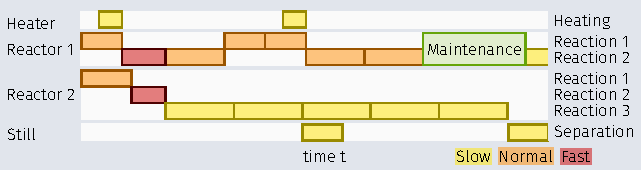
\includegraphics{schedule}
\end{frame}

\begin{frame}{Evaluating solution robustness}
    \centering
    \tikzsetnextfilename{calcp}
    %\documentclass[tikz]{standalone}
%\usepackage{tikz}
%\usepackage{pgfplots}
%\usepackage{pifont}
%\usetikzlibrary{positioning, arrows, fit, calc}
%
%\pgfmathdeclarefunction{gauss}{2}{%
%	\pgfmathparse{1/(#2*sqrt(2*pi))*exp(-((x-#1)^2)/(2*#2^2))}%
%}
%\pgfmathsetseed{2}
%
%\newcommand{\brownian}[2]{% points, advance, rand factor, options, end label
%	\draw[#1] (0,2)
%	\foreach \x in {1,...,100}
%	{
%		-- ++(0.02,0.005+rand*0.02)
%	}
%	\foreach \x in {1,...,100}
%	{
%		-- ++(0.02,0.02+rand*0.06)
%	}
%	node[right] {#2};
%}
%
%\begin{document}
	\begin{tikzpicture}[x=20mm, y=15mm ,>=stealth',bend angle=45,auto]
	%\tikzstyle{state}=[circle,thick,draw=blue!75,fill=blue!20,minimum size=6mm]
	\definecolor{mred}{RGB}{248,118,109}
	\definecolor{mblue}{RGB}{61,156,255}
	\definecolor{mgreen}{RGB}{0,186,56}
	\tikzstyle{task}=[rectangle,thick,draw=black!75,
	fill=black!20,minimum size=4mm]
	\node[draw, fit={(0,0) (2,0.5)}, inner sep=0pt, label=center:1, fill=black!20] (T1) {};
	\node[draw, fit={(2,0) (4,0.5)}, inner sep=0pt, label=center:2, fill=black!20] (T2) {};
	\node[draw, fit={(4,0) (5,0.5)}, inner sep=0pt, label=center:Maint., fill=black!30] (M) {};
	\node [inner sep=0pt](D1) at (1,0.95) {%
		$\mathcal{D}_{j,1}$:~%
		\begin{tikzpicture}
		\begin{axis}[
		width=70,
		height=70,
		domain=0:10,
		ticks=none,
		samples=100]
		\addplot [very thick,cyan!50!black] {gauss(5,1)};
		\end{axis}
		\end{tikzpicture}%
	};
	\node [inner sep=0pt] (D2) at (3,0.95){%
		$\mathcal{D}_{j,2}$:~%
		\begin{tikzpicture}
		\begin{axis}[
		width=70,
		height=70,
		domain=0:10,
		ticks=none,
		samples=100]
		\addplot [very thick,cyan!50!black] {gauss(5,2)};
		\end{axis}
		\end{tikzpicture}%
	};

\draw[<->, ultra thick]  (0,0.5) node[above]{$k$} -- (0,0) -- (5,0)
node[right]{$t$};
\draw[<->, ultra thick]  (0,4.5) node[above]{$s_j$} -- (0,1.5) -- (5,1.5)
node[right]{$t$};

\draw[dashed] (0,4.0) -- (5,4.0) node[pos=0.5, above]{$s_j^{max}$};

\draw[dotted] (2,1.5) -- (2,4.0) {};
\draw[dotted] (4,1.5) -- (4,4.0) {};
\brownian{mred}{\ding{51}}
\brownian{mblue}{\ding{55}}
\brownian{mgreen}{\ding{55}}

\draw[|-|] (2.7,2.3) -- (3.1,2.3) node[pos=0.5, below]{$\Delta t$};
\draw[|-|] (3.2,2.4) -- (3.2,3.0) node[pos=0.5, right](dsj){$d_{j,2}$}
	edge [<-, bend left] node [right] {sample} (D2);
	
\draw[|-|] (1.4,2.3) -- (1.8,2.3) node[pos=0.5, above]{$\Delta t$};
\draw[|-|] (1.3,2.0) -- (1.3,2.2) node[pos=0.5, left](dsj2){$d_{j,1}$}
	edge [<-, bend left] node [right] {} (D1);
	
\node (pf) at (4.6,3.3) {$p^f_j=\frac{2}{3}$};



	\end{tikzpicture}
%\end{document}

\end{frame}

\begin{frame}{The price of robustness}
    \centering
    \tikzsetnextfilename{price-of-rob}
    % Created by tikzDevice version 0.11 on 2018-07-30 13:32:11
% !TEX encoding = UTF-8 Unicode
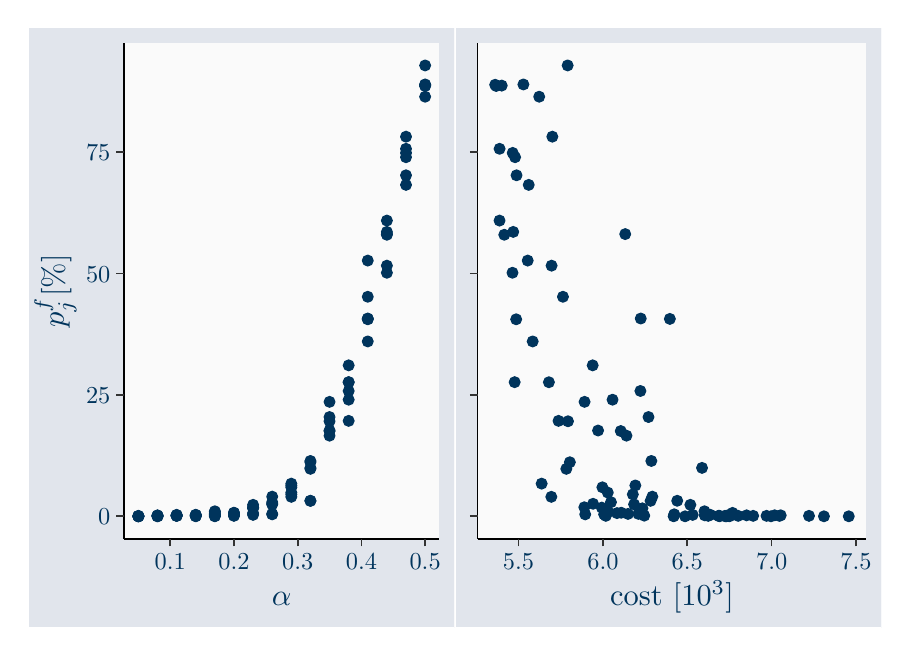
\begin{tikzpicture}[x=1pt,y=1pt]
\definecolor{fillColor}{RGB}{255,255,255}
\path[use as bounding box,fill=fillColor,fill opacity=0.00] (0,0) rectangle (308.59,216.81);
\begin{scope}
\path[clip] (  0.00,  0.00) rectangle (154.30,216.81);
\definecolor{drawColor}{RGB}{255,255,255}
\definecolor{fillColor}{RGB}{225,229,236}

\path[draw=drawColor,line width= 0.6pt,line join=round,line cap=round,fill=fillColor] (  0.00,  0.00) rectangle (154.30,216.81);
\end{scope}
\begin{scope}
\path[clip] ( 34.83, 32.09) rectangle (148.80,211.31);
\definecolor{fillColor}{gray}{0.98}

\path[fill=fillColor] ( 34.83, 32.09) rectangle (148.80,211.31);
\definecolor{drawColor}{RGB}{0,52,92}
\definecolor{fillColor}{RGB}{0,52,92}

\path[draw=drawColor,line width= 0.4pt,line join=round,line cap=round,fill=fillColor] ( 40.01, 40.41) circle (  1.96);

\path[draw=drawColor,line width= 0.4pt,line join=round,line cap=round,fill=fillColor] ( 46.92, 40.24) circle (  1.96);

\path[draw=drawColor,line width= 0.4pt,line join=round,line cap=round,fill=fillColor] ( 53.82, 40.57) circle (  1.96);

\path[draw=drawColor,line width= 0.4pt,line join=round,line cap=round,fill=fillColor] ( 60.73, 40.59) circle (  1.96);

\path[draw=drawColor,line width= 0.4pt,line join=round,line cap=round,fill=fillColor] ( 67.64, 41.82) circle (  1.96);

\path[draw=drawColor,line width= 0.4pt,line join=round,line cap=round,fill=fillColor] ( 74.54, 41.11) circle (  1.96);

\path[draw=drawColor,line width= 0.4pt,line join=round,line cap=round,fill=fillColor] ( 81.45, 43.38) circle (  1.96);

\path[draw=drawColor,line width= 0.4pt,line join=round,line cap=round,fill=fillColor] ( 88.36, 44.76) circle (  1.96);

\path[draw=drawColor,line width= 0.4pt,line join=round,line cap=round,fill=fillColor] ( 95.27, 48.16) circle (  1.96);

\path[draw=drawColor,line width= 0.4pt,line join=round,line cap=round,fill=fillColor] (102.17, 59.78) circle (  1.96);

\path[draw=drawColor,line width= 0.4pt,line join=round,line cap=round,fill=fillColor] (109.08, 74.58) circle (  1.96);

\path[draw=drawColor,line width= 0.4pt,line join=round,line cap=round,fill=fillColor] (115.99, 88.69) circle (  1.96);

\path[draw=drawColor,line width= 0.4pt,line join=round,line cap=round,fill=fillColor] (122.89,111.71) circle (  1.96);

\path[draw=drawColor,line width= 0.4pt,line join=round,line cap=round,fill=fillColor] (129.80,141.98) circle (  1.96);

\path[draw=drawColor,line width= 0.4pt,line join=round,line cap=round,fill=fillColor] (136.71,160.00) circle (  1.96);

\path[draw=drawColor,line width= 0.4pt,line join=round,line cap=round,fill=fillColor] (143.62,196.29) circle (  1.96);

\path[draw=drawColor,line width= 0.4pt,line join=round,line cap=round,fill=fillColor] ( 40.01, 40.24) circle (  1.96);

\path[draw=drawColor,line width= 0.4pt,line join=round,line cap=round,fill=fillColor] ( 46.92, 40.41) circle (  1.96);

\path[draw=drawColor,line width= 0.4pt,line join=round,line cap=round,fill=fillColor] ( 53.82, 40.61) circle (  1.96);

\path[draw=drawColor,line width= 0.4pt,line join=round,line cap=round,fill=fillColor] ( 60.73, 40.41) circle (  1.96);

\path[draw=drawColor,line width= 0.4pt,line join=round,line cap=round,fill=fillColor] ( 67.64, 40.96) circle (  1.96);

\path[draw=drawColor,line width= 0.4pt,line join=round,line cap=round,fill=fillColor] ( 74.54, 41.47) circle (  1.96);

\path[draw=drawColor,line width= 0.4pt,line join=round,line cap=round,fill=fillColor] ( 81.45, 44.39) circle (  1.96);

\path[draw=drawColor,line width= 0.4pt,line join=round,line cap=round,fill=fillColor] ( 88.36, 44.56) circle (  1.96);

\path[draw=drawColor,line width= 0.4pt,line join=round,line cap=round,fill=fillColor] ( 95.27, 51.39) circle (  1.96);

\path[draw=drawColor,line width= 0.4pt,line join=round,line cap=round,fill=fillColor] (102.17, 57.39) circle (  1.96);

\path[draw=drawColor,line width= 0.4pt,line join=round,line cap=round,fill=fillColor] (109.08, 71.24) circle (  1.96);

\path[draw=drawColor,line width= 0.4pt,line join=round,line cap=round,fill=fillColor] (115.99, 88.71) circle (  1.96);

\path[draw=drawColor,line width= 0.4pt,line join=round,line cap=round,fill=fillColor] (122.89,111.43) circle (  1.96);

\path[draw=drawColor,line width= 0.4pt,line join=round,line cap=round,fill=fillColor] (129.80,128.25) circle (  1.96);

\path[draw=drawColor,line width= 0.4pt,line join=round,line cap=round,fill=fillColor] (136.71,170.00) circle (  1.96);

\path[draw=drawColor,line width= 0.4pt,line join=round,line cap=round,fill=fillColor] (143.62,195.73) circle (  1.96);

\path[draw=drawColor,line width= 0.4pt,line join=round,line cap=round,fill=fillColor] ( 40.01, 40.24) circle (  1.96);

\path[draw=drawColor,line width= 0.4pt,line join=round,line cap=round,fill=fillColor] ( 46.92, 40.48) circle (  1.96);

\path[draw=drawColor,line width= 0.4pt,line join=round,line cap=round,fill=fillColor] ( 53.82, 40.43) circle (  1.96);

\path[draw=drawColor,line width= 0.4pt,line join=round,line cap=round,fill=fillColor] ( 60.73, 40.24) circle (  1.96);

\path[draw=drawColor,line width= 0.4pt,line join=round,line cap=round,fill=fillColor] ( 67.64, 40.24) circle (  1.96);

\path[draw=drawColor,line width= 0.4pt,line join=round,line cap=round,fill=fillColor] ( 74.54, 41.54) circle (  1.96);

\path[draw=drawColor,line width= 0.4pt,line join=round,line cap=round,fill=fillColor] ( 81.45, 40.76) circle (  1.96);

\path[draw=drawColor,line width= 0.4pt,line join=round,line cap=round,fill=fillColor] ( 88.36, 45.34) circle (  1.96);

\path[draw=drawColor,line width= 0.4pt,line join=round,line cap=round,fill=fillColor] ( 95.27, 47.28) circle (  1.96);

\path[draw=drawColor,line width= 0.4pt,line join=round,line cap=round,fill=fillColor] (102.17, 45.85) circle (  1.96);

\path[draw=drawColor,line width= 0.4pt,line join=round,line cap=round,fill=fillColor] (109.08, 81.60) circle (  1.96);

\path[draw=drawColor,line width= 0.4pt,line join=round,line cap=round,fill=fillColor] (115.99, 82.38) circle (  1.96);

\path[draw=drawColor,line width= 0.4pt,line join=round,line cap=round,fill=fillColor] (122.89,103.43) circle (  1.96);

\path[draw=drawColor,line width= 0.4pt,line join=round,line cap=round,fill=fillColor] (129.80,147.10) circle (  1.96);

\path[draw=drawColor,line width= 0.4pt,line join=round,line cap=round,fill=fillColor] (136.71,173.04) circle (  1.96);

\path[draw=drawColor,line width= 0.4pt,line join=round,line cap=round,fill=fillColor] (143.62,191.86) circle (  1.96);

\path[draw=drawColor,line width= 0.4pt,line join=round,line cap=round,fill=fillColor] ( 40.01, 40.24) circle (  1.96);

\path[draw=drawColor,line width= 0.4pt,line join=round,line cap=round,fill=fillColor] ( 46.92, 40.59) circle (  1.96);

\path[draw=drawColor,line width= 0.4pt,line join=round,line cap=round,fill=fillColor] ( 53.82, 40.41) circle (  1.96);

\path[draw=drawColor,line width= 0.4pt,line join=round,line cap=round,fill=fillColor] ( 60.73, 40.41) circle (  1.96);

\path[draw=drawColor,line width= 0.4pt,line join=round,line cap=round,fill=fillColor] ( 67.64, 40.41) circle (  1.96);

\path[draw=drawColor,line width= 0.4pt,line join=round,line cap=round,fill=fillColor] ( 74.54, 40.59) circle (  1.96);

\path[draw=drawColor,line width= 0.4pt,line join=round,line cap=round,fill=fillColor] ( 81.45, 43.51) circle (  1.96);

\path[draw=drawColor,line width= 0.4pt,line join=round,line cap=round,fill=fillColor] ( 88.36, 40.95) circle (  1.96);

\path[draw=drawColor,line width= 0.4pt,line join=round,line cap=round,fill=fillColor] ( 95.27, 52.05) circle (  1.96);

\path[draw=drawColor,line width= 0.4pt,line join=round,line cap=round,fill=fillColor] (102.17, 57.74) circle (  1.96);

\path[draw=drawColor,line width= 0.4pt,line join=round,line cap=round,fill=fillColor] (109.08, 71.05) circle (  1.96);

\path[draw=drawColor,line width= 0.4pt,line join=round,line cap=round,fill=fillColor] (115.99, 94.79) circle (  1.96);

\path[draw=drawColor,line width= 0.4pt,line join=round,line cap=round,fill=fillColor] (122.89,132.65) circle (  1.96);

\path[draw=drawColor,line width= 0.4pt,line join=round,line cap=round,fill=fillColor] (129.80,130.81) circle (  1.96);

\path[draw=drawColor,line width= 0.4pt,line join=round,line cap=round,fill=fillColor] (136.71,177.42) circle (  1.96);

\path[draw=drawColor,line width= 0.4pt,line join=round,line cap=round,fill=fillColor] (143.62,195.88) circle (  1.96);

\path[draw=drawColor,line width= 0.4pt,line join=round,line cap=round,fill=fillColor] ( 40.01, 40.24) circle (  1.96);

\path[draw=drawColor,line width= 0.4pt,line join=round,line cap=round,fill=fillColor] ( 46.92, 40.41) circle (  1.96);

\path[draw=drawColor,line width= 0.4pt,line join=round,line cap=round,fill=fillColor] ( 53.82, 40.77) circle (  1.96);

\path[draw=drawColor,line width= 0.4pt,line join=round,line cap=round,fill=fillColor] ( 60.73, 40.76) circle (  1.96);

\path[draw=drawColor,line width= 0.4pt,line join=round,line cap=round,fill=fillColor] ( 67.64, 41.12) circle (  1.96);

\path[draw=drawColor,line width= 0.4pt,line join=round,line cap=round,fill=fillColor] ( 74.54, 40.41) circle (  1.96);

\path[draw=drawColor,line width= 0.4pt,line join=round,line cap=round,fill=fillColor] ( 81.45, 41.39) circle (  1.96);

\path[draw=drawColor,line width= 0.4pt,line join=round,line cap=round,fill=fillColor] ( 88.36, 47.35) circle (  1.96);

\path[draw=drawColor,line width= 0.4pt,line join=round,line cap=round,fill=fillColor] ( 95.27, 50.72) circle (  1.96);

\path[draw=drawColor,line width= 0.4pt,line join=round,line cap=round,fill=fillColor] (102.17, 60.24) circle (  1.96);

\path[draw=drawColor,line width= 0.4pt,line join=round,line cap=round,fill=fillColor] (109.08, 69.38) circle (  1.96);

\path[draw=drawColor,line width= 0.4pt,line join=round,line cap=round,fill=fillColor] (115.99, 74.73) circle (  1.96);

\path[draw=drawColor,line width= 0.4pt,line join=round,line cap=round,fill=fillColor] (122.89,119.57) circle (  1.96);

\path[draw=drawColor,line width= 0.4pt,line join=round,line cap=round,fill=fillColor] (129.80,143.01) circle (  1.96);

\path[draw=drawColor,line width= 0.4pt,line join=round,line cap=round,fill=fillColor] (136.71,171.55) circle (  1.96);

\path[draw=drawColor,line width= 0.4pt,line join=round,line cap=round,fill=fillColor] (143.62,196.18) circle (  1.96);

\path[draw=drawColor,line width= 0.4pt,line join=round,line cap=round,fill=fillColor] ( 40.01, 40.24) circle (  1.96);

\path[draw=drawColor,line width= 0.4pt,line join=round,line cap=round,fill=fillColor] ( 46.92, 40.24) circle (  1.96);

\path[draw=drawColor,line width= 0.4pt,line join=round,line cap=round,fill=fillColor] ( 53.82, 40.41) circle (  1.96);

\path[draw=drawColor,line width= 0.4pt,line join=round,line cap=round,fill=fillColor] ( 60.73, 40.76) circle (  1.96);

\path[draw=drawColor,line width= 0.4pt,line join=round,line cap=round,fill=fillColor] ( 67.64, 42.06) circle (  1.96);

\path[draw=drawColor,line width= 0.4pt,line join=round,line cap=round,fill=fillColor] ( 74.54, 40.94) circle (  1.96);

\path[draw=drawColor,line width= 0.4pt,line join=round,line cap=round,fill=fillColor] ( 81.45, 43.12) circle (  1.96);

\path[draw=drawColor,line width= 0.4pt,line join=round,line cap=round,fill=fillColor] ( 88.36, 41.11) circle (  1.96);

\path[draw=drawColor,line width= 0.4pt,line join=round,line cap=round,fill=fillColor] ( 95.27, 48.82) circle (  1.96);

\path[draw=drawColor,line width= 0.4pt,line join=round,line cap=round,fill=fillColor] (102.17, 45.83) circle (  1.96);

\path[draw=drawColor,line width= 0.4pt,line join=round,line cap=round,fill=fillColor] (109.08, 76.11) circle (  1.96);

\path[draw=drawColor,line width= 0.4pt,line join=round,line cap=round,fill=fillColor] (115.99, 85.53) circle (  1.96);

\path[draw=drawColor,line width= 0.4pt,line join=round,line cap=round,fill=fillColor] (122.89,111.57) circle (  1.96);

\path[draw=drawColor,line width= 0.4pt,line join=round,line cap=round,fill=fillColor] (129.80,142.22) circle (  1.96);

\path[draw=drawColor,line width= 0.4pt,line join=round,line cap=round,fill=fillColor] (136.71,163.46) circle (  1.96);

\path[draw=drawColor,line width= 0.4pt,line join=round,line cap=round,fill=fillColor] (143.62,203.16) circle (  1.96);
\end{scope}
\begin{scope}
\path[clip] (  0.00,  0.00) rectangle (308.59,216.81);
\definecolor{drawColor}{RGB}{0,0,0}

\path[draw=drawColor,line width= 0.6pt,line join=round] ( 34.83, 32.09) --
	( 34.83,211.31);
\end{scope}
\begin{scope}
\path[clip] (  0.00,  0.00) rectangle (308.59,216.81);
\definecolor{drawColor}{RGB}{0,52,92}

\node[text=drawColor,anchor=base east,inner sep=0pt, outer sep=0pt, scale=  0.88] at ( 29.88, 37.21) {0};

\node[text=drawColor,anchor=base east,inner sep=0pt, outer sep=0pt, scale=  0.88] at ( 29.88, 81.05) {25};

\node[text=drawColor,anchor=base east,inner sep=0pt, outer sep=0pt, scale=  0.88] at ( 29.88,124.89) {50};

\node[text=drawColor,anchor=base east,inner sep=0pt, outer sep=0pt, scale=  0.88] at ( 29.88,168.74) {75};
\end{scope}
\begin{scope}
\path[clip] (  0.00,  0.00) rectangle (308.59,216.81);
\definecolor{drawColor}{gray}{0.20}

\path[draw=drawColor,line width= 0.6pt,line join=round] ( 32.08, 40.24) --
	( 34.83, 40.24);

\path[draw=drawColor,line width= 0.6pt,line join=round] ( 32.08, 84.08) --
	( 34.83, 84.08);

\path[draw=drawColor,line width= 0.6pt,line join=round] ( 32.08,127.92) --
	( 34.83,127.92);

\path[draw=drawColor,line width= 0.6pt,line join=round] ( 32.08,171.77) --
	( 34.83,171.77);
\end{scope}
\begin{scope}
\path[clip] (  0.00,  0.00) rectangle (308.59,216.81);
\definecolor{drawColor}{RGB}{0,0,0}

\path[draw=drawColor,line width= 0.6pt,line join=round] ( 34.83, 32.09) --
	(148.80, 32.09);
\end{scope}
\begin{scope}
\path[clip] (  0.00,  0.00) rectangle (308.59,216.81);
\definecolor{drawColor}{gray}{0.20}

\path[draw=drawColor,line width= 0.6pt,line join=round] ( 51.52, 29.34) --
	( 51.52, 32.09);

\path[draw=drawColor,line width= 0.6pt,line join=round] ( 74.54, 29.34) --
	( 74.54, 32.09);

\path[draw=drawColor,line width= 0.6pt,line join=round] ( 97.57, 29.34) --
	( 97.57, 32.09);

\path[draw=drawColor,line width= 0.6pt,line join=round] (120.59, 29.34) --
	(120.59, 32.09);

\path[draw=drawColor,line width= 0.6pt,line join=round] (143.62, 29.34) --
	(143.62, 32.09);
\end{scope}
\begin{scope}
\path[clip] (  0.00,  0.00) rectangle (308.59,216.81);
\definecolor{drawColor}{RGB}{0,52,92}

\node[text=drawColor,anchor=base,inner sep=0pt, outer sep=0pt, scale=  0.88] at ( 51.52, 21.08) {0.1};

\node[text=drawColor,anchor=base,inner sep=0pt, outer sep=0pt, scale=  0.88] at ( 74.54, 21.08) {0.2};

\node[text=drawColor,anchor=base,inner sep=0pt, outer sep=0pt, scale=  0.88] at ( 97.57, 21.08) {0.3};

\node[text=drawColor,anchor=base,inner sep=0pt, outer sep=0pt, scale=  0.88] at (120.59, 21.08) {0.4};

\node[text=drawColor,anchor=base,inner sep=0pt, outer sep=0pt, scale=  0.88] at (143.62, 21.08) {0.5};
\end{scope}
\begin{scope}
\path[clip] (  0.00,  0.00) rectangle (308.59,216.81);
\definecolor{drawColor}{RGB}{0,52,92}

\node[text=drawColor,anchor=base,inner sep=0pt, outer sep=0pt, scale=  1.10] at ( 91.81,  8.00) {$\alpha$};
\end{scope}
\begin{scope}
\path[clip] (  0.00,  0.00) rectangle (308.59,216.81);
\definecolor{drawColor}{RGB}{0,52,92}

\node[text=drawColor,rotate= 90.00,anchor=base,inner sep=0pt, outer sep=0pt, scale=  1.10] at ( 13.08,121.70) {$p^f_{j} [\%]$};
\end{scope}
\begin{scope}
\path[clip] (154.30,  0.00) rectangle (308.59,216.81);
\definecolor{drawColor}{RGB}{255,255,255}
\definecolor{fillColor}{RGB}{225,229,236}

\path[draw=drawColor,line width= 0.6pt,line join=round,line cap=round,fill=fillColor] (154.30,  0.00) rectangle (308.59,216.81);
\end{scope}
\begin{scope}
\path[clip] (162.55, 32.09) rectangle (303.09,211.31);
\definecolor{fillColor}{gray}{0.98}

\path[fill=fillColor] (162.55, 32.09) rectangle (303.09,211.31);
\definecolor{drawColor}{RGB}{0,52,92}
\definecolor{fillColor}{RGB}{0,52,92}

\path[draw=drawColor,line width= 0.4pt,line join=round,line cap=round,fill=fillColor] (262.15, 40.41) circle (  1.96);

\path[draw=drawColor,line width= 0.4pt,line join=round,line cap=round,fill=fillColor] (296.70, 40.24) circle (  1.96);

\path[draw=drawColor,line width= 0.4pt,line join=round,line cap=round,fill=fillColor] (252.94, 40.57) circle (  1.96);

\path[draw=drawColor,line width= 0.4pt,line join=round,line cap=round,fill=fillColor] (272.11, 40.59) circle (  1.96);

\path[draw=drawColor,line width= 0.4pt,line join=round,line cap=round,fill=fillColor] (209.78, 41.82) circle (  1.96);

\path[draw=drawColor,line width= 0.4pt,line join=round,line cap=round,fill=fillColor] (216.93, 41.11) circle (  1.96);

\path[draw=drawColor,line width= 0.4pt,line join=round,line cap=round,fill=fillColor] (207.46, 43.38) circle (  1.96);

\path[draw=drawColor,line width= 0.4pt,line join=round,line cap=round,fill=fillColor] (204.30, 44.76) circle (  1.96);

\path[draw=drawColor,line width= 0.4pt,line join=round,line cap=round,fill=fillColor] (218.67, 48.16) circle (  1.96);

\path[draw=drawColor,line width= 0.4pt,line join=round,line cap=round,fill=fillColor] (195.91, 59.78) circle (  1.96);

\path[draw=drawColor,line width= 0.4pt,line join=round,line cap=round,fill=fillColor] (195.24, 74.58) circle (  1.96);

\path[draw=drawColor,line width= 0.4pt,line join=round,line cap=round,fill=fillColor] (188.34, 88.69) circle (  1.96);

\path[draw=drawColor,line width= 0.4pt,line join=round,line cap=round,fill=fillColor] (221.53,111.71) circle (  1.96);

\path[draw=drawColor,line width= 0.4pt,line join=round,line cap=round,fill=fillColor] (172.22,141.98) circle (  1.96);

\path[draw=drawColor,line width= 0.4pt,line join=round,line cap=round,fill=fillColor] (181.05,160.00) circle (  1.96);

\path[draw=drawColor,line width= 0.4pt,line join=round,line cap=round,fill=fillColor] (179.13,196.29) circle (  1.96);

\path[draw=drawColor,line width= 0.4pt,line join=round,line cap=round,fill=fillColor] (287.73, 40.24) circle (  1.96);

\path[draw=drawColor,line width= 0.4pt,line join=round,line cap=round,fill=fillColor] (271.60, 40.41) circle (  1.96);

\path[draw=drawColor,line width= 0.4pt,line join=round,line cap=round,fill=fillColor] (269.92, 40.61) circle (  1.96);

\path[draw=drawColor,line width= 0.4pt,line join=round,line cap=round,fill=fillColor] (249.64, 40.41) circle (  1.96);

\path[draw=drawColor,line width= 0.4pt,line join=round,line cap=round,fill=fillColor] (233.62, 40.96) circle (  1.96);

\path[draw=drawColor,line width= 0.4pt,line join=round,line cap=round,fill=fillColor] (254.71, 41.47) circle (  1.96);

\path[draw=drawColor,line width= 0.4pt,line join=round,line cap=round,fill=fillColor] (239.46, 44.39) circle (  1.96);

\path[draw=drawColor,line width= 0.4pt,line join=round,line cap=round,fill=fillColor] (219.13, 44.56) circle (  1.96);

\path[draw=drawColor,line width= 0.4pt,line join=round,line cap=round,fill=fillColor] (219.58, 51.39) circle (  1.96);

\path[draw=drawColor,line width= 0.4pt,line join=round,line cap=round,fill=fillColor] (194.64, 57.39) circle (  1.96);

\path[draw=drawColor,line width= 0.4pt,line join=round,line cap=round,fill=fillColor] (206.11, 71.24) circle (  1.96);

\path[draw=drawColor,line width= 0.4pt,line join=round,line cap=round,fill=fillColor] (175.97, 88.71) circle (  1.96);

\path[draw=drawColor,line width= 0.4pt,line join=round,line cap=round,fill=fillColor] (176.52,111.43) circle (  1.96);

\path[draw=drawColor,line width= 0.4pt,line join=round,line cap=round,fill=fillColor] (175.18,128.25) circle (  1.96);

\path[draw=drawColor,line width= 0.4pt,line join=round,line cap=round,fill=fillColor] (176.13,170.00) circle (  1.96);

\path[draw=drawColor,line width= 0.4pt,line join=round,line cap=round,fill=fillColor] (169.30,195.73) circle (  1.96);

\path[draw=drawColor,line width= 0.4pt,line join=round,line cap=round,fill=fillColor] (237.56, 40.24) circle (  1.96);

\path[draw=drawColor,line width= 0.4pt,line join=round,line cap=round,fill=fillColor] (222.80, 40.48) circle (  1.96);

\path[draw=drawColor,line width= 0.4pt,line join=round,line cap=round,fill=fillColor] (249.94, 40.43) circle (  1.96);

\path[draw=drawColor,line width= 0.4pt,line join=round,line cap=round,fill=fillColor] (250.02, 40.24) circle (  1.96);

\path[draw=drawColor,line width= 0.4pt,line join=round,line cap=round,fill=fillColor] (233.42, 40.24) circle (  1.96);

\path[draw=drawColor,line width= 0.4pt,line join=round,line cap=round,fill=fillColor] (214.49, 41.54) circle (  1.96);

\path[draw=drawColor,line width= 0.4pt,line join=round,line cap=round,fill=fillColor] (240.30, 40.76) circle (  1.96);

\path[draw=drawColor,line width= 0.4pt,line join=round,line cap=round,fill=fillColor] (210.77, 45.34) circle (  1.96);

\path[draw=drawColor,line width= 0.4pt,line join=round,line cap=round,fill=fillColor] (189.22, 47.28) circle (  1.96);

\path[draw=drawColor,line width= 0.4pt,line join=round,line cap=round,fill=fillColor] (234.71, 45.85) circle (  1.96);

\path[draw=drawColor,line width= 0.4pt,line join=round,line cap=round,fill=fillColor] (201.23, 81.60) circle (  1.96);

\path[draw=drawColor,line width= 0.4pt,line join=round,line cap=round,fill=fillColor] (211.34, 82.38) circle (  1.96);

\path[draw=drawColor,line width= 0.4pt,line join=round,line cap=round,fill=fillColor] (182.48,103.43) circle (  1.96);

\path[draw=drawColor,line width= 0.4pt,line join=round,line cap=round,fill=fillColor] (170.51,147.10) circle (  1.96);

\path[draw=drawColor,line width= 0.4pt,line join=round,line cap=round,fill=fillColor] (170.52,173.04) circle (  1.96);

\path[draw=drawColor,line width= 0.4pt,line join=round,line cap=round,fill=fillColor] (184.84,191.86) circle (  1.96);

\path[draw=drawColor,line width= 0.4pt,line join=round,line cap=round,fill=fillColor] (253.57, 40.24) circle (  1.96);

\path[draw=drawColor,line width= 0.4pt,line join=round,line cap=round,fill=fillColor] (259.78, 40.59) circle (  1.96);

\path[draw=drawColor,line width= 0.4pt,line join=round,line cap=round,fill=fillColor] (256.74, 40.41) circle (  1.96);

\path[draw=drawColor,line width= 0.4pt,line join=round,line cap=round,fill=fillColor] (251.96, 40.41) circle (  1.96);

\path[draw=drawColor,line width= 0.4pt,line join=round,line cap=round,fill=fillColor] (245.92, 40.41) circle (  1.96);

\path[draw=drawColor,line width= 0.4pt,line join=round,line cap=round,fill=fillColor] (244.67, 40.59) circle (  1.96);

\path[draw=drawColor,line width= 0.4pt,line join=round,line cap=round,fill=fillColor] (201.15, 43.51) circle (  1.96);

\path[draw=drawColor,line width= 0.4pt,line join=round,line cap=round,fill=fillColor] (208.30, 40.95) circle (  1.96);

\path[draw=drawColor,line width= 0.4pt,line join=round,line cap=round,fill=fillColor] (185.72, 52.05) circle (  1.96);

\path[draw=drawColor,line width= 0.4pt,line join=round,line cap=round,fill=fillColor] (243.68, 57.74) circle (  1.96);

\path[draw=drawColor,line width= 0.4pt,line join=round,line cap=round,fill=fillColor] (214.31, 71.05) circle (  1.96);

\path[draw=drawColor,line width= 0.4pt,line join=round,line cap=round,fill=fillColor] (204.16, 94.79) circle (  1.96);

\path[draw=drawColor,line width= 0.4pt,line join=round,line cap=round,fill=fillColor] (180.68,132.65) circle (  1.96);

\path[draw=drawColor,line width= 0.4pt,line join=round,line cap=round,fill=fillColor] (189.31,130.81) circle (  1.96);

\path[draw=drawColor,line width= 0.4pt,line join=round,line cap=round,fill=fillColor] (189.59,177.42) circle (  1.96);

\path[draw=drawColor,line width= 0.4pt,line join=round,line cap=round,fill=fillColor] (171.30,195.88) circle (  1.96);

\path[draw=drawColor,line width= 0.4pt,line join=round,line cap=round,fill=fillColor] (268.60, 40.24) circle (  1.96);

\path[draw=drawColor,line width= 0.4pt,line join=round,line cap=round,fill=fillColor] (266.99, 40.41) circle (  1.96);

\path[draw=drawColor,line width= 0.4pt,line join=round,line cap=round,fill=fillColor] (233.66, 40.77) circle (  1.96);

\path[draw=drawColor,line width= 0.4pt,line join=round,line cap=round,fill=fillColor] (244.92, 40.76) circle (  1.96);

\path[draw=drawColor,line width= 0.4pt,line join=round,line cap=round,fill=fillColor] (220.67, 41.12) circle (  1.96);

\path[draw=drawColor,line width= 0.4pt,line join=round,line cap=round,fill=fillColor] (208.92, 40.41) circle (  1.96);

\path[draw=drawColor,line width= 0.4pt,line join=round,line cap=round,fill=fillColor] (212.95, 41.39) circle (  1.96);

\path[draw=drawColor,line width= 0.4pt,line join=round,line cap=round,fill=fillColor] (225.72, 47.35) circle (  1.96);

\path[draw=drawColor,line width= 0.4pt,line join=round,line cap=round,fill=fillColor] (207.67, 50.72) circle (  1.96);

\path[draw=drawColor,line width= 0.4pt,line join=round,line cap=round,fill=fillColor] (225.36, 60.24) circle (  1.96);

\path[draw=drawColor,line width= 0.4pt,line join=round,line cap=round,fill=fillColor] (216.37, 69.38) circle (  1.96);

\path[draw=drawColor,line width= 0.4pt,line join=round,line cap=round,fill=fillColor] (191.82, 74.73) circle (  1.96);

\path[draw=drawColor,line width= 0.4pt,line join=round,line cap=round,fill=fillColor] (193.42,119.57) circle (  1.96);

\path[draw=drawColor,line width= 0.4pt,line join=round,line cap=round,fill=fillColor] (175.45,143.01) circle (  1.96);

\path[draw=drawColor,line width= 0.4pt,line join=round,line cap=round,fill=fillColor] (175.26,171.55) circle (  1.96);

\path[draw=drawColor,line width= 0.4pt,line join=round,line cap=round,fill=fillColor] (168.93,196.18) circle (  1.96);

\path[draw=drawColor,line width= 0.4pt,line join=round,line cap=round,fill=fillColor] (252.45, 40.24) circle (  1.96);

\path[draw=drawColor,line width= 0.4pt,line join=round,line cap=round,fill=fillColor] (252.14, 40.24) circle (  1.96);

\path[draw=drawColor,line width= 0.4pt,line join=round,line cap=round,fill=fillColor] (282.33, 40.41) circle (  1.96);

\path[draw=drawColor,line width= 0.4pt,line join=round,line cap=round,fill=fillColor] (246.71, 40.76) circle (  1.96);

\path[draw=drawColor,line width= 0.4pt,line join=round,line cap=round,fill=fillColor] (244.57, 42.06) circle (  1.96);

\path[draw=drawColor,line width= 0.4pt,line join=round,line cap=round,fill=fillColor] (201.47, 40.94) circle (  1.96);

\path[draw=drawColor,line width= 0.4pt,line join=round,line cap=round,fill=fillColor] (222.14, 43.12) circle (  1.96);

\path[draw=drawColor,line width= 0.4pt,line join=round,line cap=round,fill=fillColor] (208.96, 41.11) circle (  1.96);

\path[draw=drawColor,line width= 0.4pt,line join=round,line cap=round,fill=fillColor] (209.62, 48.82) circle (  1.96);

\path[draw=drawColor,line width= 0.4pt,line join=round,line cap=round,fill=fillColor] (225.09, 45.83) circle (  1.96);

\path[draw=drawColor,line width= 0.4pt,line join=round,line cap=round,fill=fillColor] (224.33, 76.11) circle (  1.96);

\path[draw=drawColor,line width= 0.4pt,line join=round,line cap=round,fill=fillColor] (221.41, 85.53) circle (  1.96);

\path[draw=drawColor,line width= 0.4pt,line join=round,line cap=round,fill=fillColor] (232.05,111.57) circle (  1.96);

\path[draw=drawColor,line width= 0.4pt,line join=round,line cap=round,fill=fillColor] (215.92,142.22) circle (  1.96);

\path[draw=drawColor,line width= 0.4pt,line join=round,line cap=round,fill=fillColor] (176.65,163.46) circle (  1.96);

\path[draw=drawColor,line width= 0.4pt,line join=round,line cap=round,fill=fillColor] (195.12,203.16) circle (  1.96);
\end{scope}
\begin{scope}
\path[clip] (  0.00,  0.00) rectangle (308.59,216.81);
\definecolor{drawColor}{RGB}{0,0,0}

\path[draw=drawColor,line width= 0.6pt,line join=round] (162.55, 32.09) --
	(162.55,211.31);
\end{scope}
\begin{scope}
\path[clip] (  0.00,  0.00) rectangle (308.59,216.81);
\definecolor{drawColor}{gray}{0.20}

\path[draw=drawColor,line width= 0.6pt,line join=round] (159.80, 40.24) --
	(162.55, 40.24);

\path[draw=drawColor,line width= 0.6pt,line join=round] (159.80, 84.08) --
	(162.55, 84.08);

\path[draw=drawColor,line width= 0.6pt,line join=round] (159.80,127.92) --
	(162.55,127.92);

\path[draw=drawColor,line width= 0.6pt,line join=round] (159.80,171.77) --
	(162.55,171.77);
\end{scope}
\begin{scope}
\path[clip] (  0.00,  0.00) rectangle (308.59,216.81);
\definecolor{drawColor}{RGB}{0,0,0}

\path[draw=drawColor,line width= 0.6pt,line join=round] (162.55, 32.09) --
	(303.09, 32.09);
\end{scope}
\begin{scope}
\path[clip] (  0.00,  0.00) rectangle (308.59,216.81);
\definecolor{drawColor}{gray}{0.20}

\path[draw=drawColor,line width= 0.6pt,line join=round] (177.37, 29.34) --
	(177.37, 32.09);

\path[draw=drawColor,line width= 0.6pt,line join=round] (207.86, 29.34) --
	(207.86, 32.09);

\path[draw=drawColor,line width= 0.6pt,line join=round] (238.34, 29.34) --
	(238.34, 32.09);

\path[draw=drawColor,line width= 0.6pt,line join=round] (268.83, 29.34) --
	(268.83, 32.09);

\path[draw=drawColor,line width= 0.6pt,line join=round] (299.31, 29.34) --
	(299.31, 32.09);
\end{scope}
\begin{scope}
\path[clip] (  0.00,  0.00) rectangle (308.59,216.81);
\definecolor{drawColor}{RGB}{0,52,92}

\node[text=drawColor,anchor=base,inner sep=0pt, outer sep=0pt, scale=  0.88] at (177.37, 21.08) {5.5};

\node[text=drawColor,anchor=base,inner sep=0pt, outer sep=0pt, scale=  0.88] at (207.86, 21.08) {6.0};

\node[text=drawColor,anchor=base,inner sep=0pt, outer sep=0pt, scale=  0.88] at (238.34, 21.08) {6.5};

\node[text=drawColor,anchor=base,inner sep=0pt, outer sep=0pt, scale=  0.88] at (268.83, 21.08) {7.0};

\node[text=drawColor,anchor=base,inner sep=0pt, outer sep=0pt, scale=  0.88] at (299.31, 21.08) {7.5};
\end{scope}
\begin{scope}
\path[clip] (  0.00,  0.00) rectangle (308.59,216.81);
\definecolor{drawColor}{RGB}{0,52,92}

\node[text=drawColor,anchor=base,inner sep=0pt, outer sep=0pt, scale=  1.10] at (232.82,  8.00) {cost [$10^3$]};
\end{scope}
\end{tikzpicture}

\end{frame}


\begin{frame}{Choosing $\alpha$ is its own optimization problem}
     We optimize $\alpha$ by solving
    \begin{equation*}
    \min_{\alpha} c^*(\alpha) + \sum_{j} p^f_{j}(\alpha)\cdot c_{j}^f
    \end{equation*}
    \begin{itemize}
        \item $c^*(\alpha)$ is the objective value of a MILP solution given $\alpha$.
        \item $p^f_j(\alpha)$ is the corresponding probability of failure (of
            unit $j$).
        \item $c_j^f$ is the cost of an unexpected failure.
    \end{itemize}
    \visible<2->{
        \begin{exampleblock}{Idea: Use Bayesian Optimization (BO)}
            Both $c^*$ and $p^f_j$ can be viewed as expensive black box functions.
            BO is very suitable for this setting \citep{Jones1998}.
        \end{exampleblock}
    }
\end{frame}


\begin{frame}{Saving time: a deterministic approximation}
\only<1>{
    \begin{alertblock}{Assumption}
        Only the health model depends on $\tilde{d}_{j,k}$ and $\tilde{d}_{j,k} \geq 0.$
    \end{alertblock}
    Then we can prove that a solution to
    \begin{equation*}
    \label{eq:bigD}
    \begin{aligned}
    & \underset{\bm{x},\bm{m}, \bm{h}}{\text{min}}
    && \text{cost}(\bm{x},
        \bm{m},{\color{imperialAlertText}\text{\sout{$\bm{h}$}}})\\
    & \text{s.t.}
    && \text{process model, maint. model}(\bm{x}, \bm{m},{\color{imperialAlertText}\text{\sout{$\bm{h}$}}})
    &&& \\
    &
    && s_{j,t} \leq s_{j}^{max}
    &&& \forall t, j \in J\\
    &
    && s_{j,t} =
    \begin{cases}
        s_{j,t-1} + {\sum\limits_{k \in
        \mathcal{K}}{x_{j,k,t}\cdot}}
        {\color{imperialAlertText}{d}^{max}_{j,k}}, & \text{if } m_{j,t} = 0\\
    s_{j}^{0}, & \text{otherwise}
    \end{cases}
    &&& \forall t, j \in J\\
    \end{aligned}
    \end{equation*}
    with $d_{j,k}^{max} = \max_{\mathcal{U}} \tilde{d}_{j,k}$ is also feasible in the robust problem.
}
\only<2>{
    \tikzsetnextfilename{det-vs-rob}
    % Created by tikzDevice version 0.11 on 2018-07-30 13:33:02
% !TEX encoding = UTF-8 Unicode
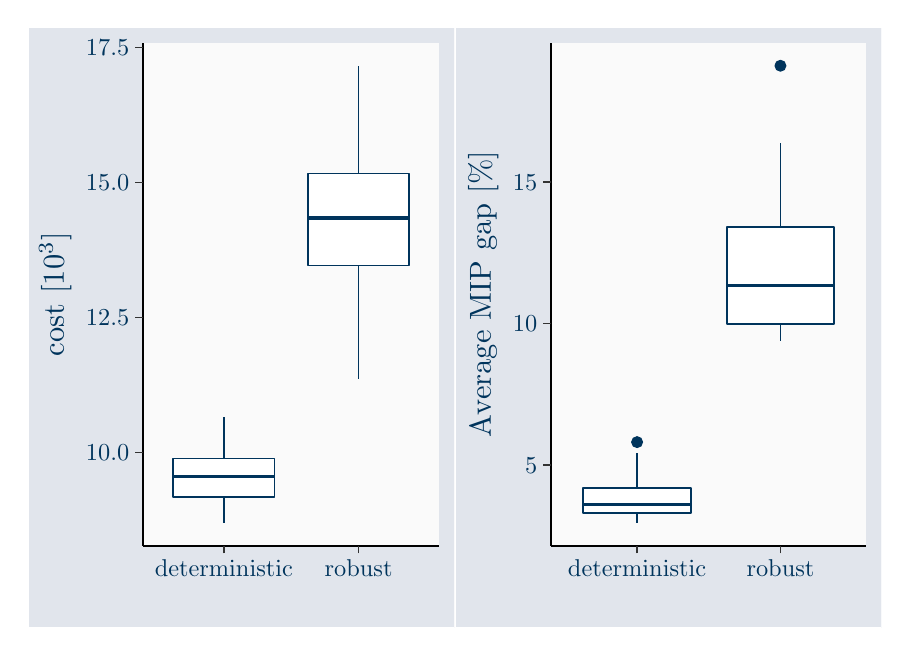
\begin{tikzpicture}[x=1pt,y=1pt]
\definecolor{fillColor}{RGB}{255,255,255}
\path[use as bounding box,fill=fillColor,fill opacity=0.00] (0,0) rectangle (308.59,216.81);
\begin{scope}
\path[clip] (  0.00,  0.00) rectangle (154.30,216.81);
\definecolor{drawColor}{RGB}{255,255,255}
\definecolor{fillColor}{RGB}{225,229,236}

\path[draw=drawColor,line width= 0.6pt,line join=round,line cap=round,fill=fillColor] (  0.00,  0.00) rectangle (154.30,216.81);
\end{scope}
\begin{scope}
\path[clip] ( 41.67, 29.59) rectangle (148.80,211.31);
\definecolor{fillColor}{gray}{0.98}

\path[fill=fillColor] ( 41.67, 29.59) rectangle (148.80,211.31);
\definecolor{drawColor}{RGB}{0,52,92}

\path[draw=drawColor,line width= 0.6pt,line join=round] ( 70.89, 61.17) -- ( 70.89, 76.26);

\path[draw=drawColor,line width= 0.6pt,line join=round] ( 70.89, 47.21) -- ( 70.89, 37.85);
\definecolor{fillColor}{RGB}{255,255,255}

\path[draw=drawColor,line width= 0.6pt,line join=round,line cap=round,fill=fillColor] ( 52.63, 61.17) --
	( 52.63, 47.21) --
	( 89.15, 47.21) --
	( 89.15, 61.17) --
	( 52.63, 61.17) --
	cycle;

\path[draw=drawColor,line width= 1.1pt,line join=round] ( 52.63, 54.77) -- ( 89.15, 54.77);

\path[draw=drawColor,line width= 0.6pt,line join=round] (119.58,164.06) -- (119.58,203.05);

\path[draw=drawColor,line width= 0.6pt,line join=round] (119.58,130.88) -- (119.58, 89.89);

\path[draw=drawColor,line width= 0.6pt,line join=round,line cap=round,fill=fillColor] (101.32,164.06) --
	(101.32,130.88) --
	(137.84,130.88) --
	(137.84,164.06) --
	(101.32,164.06) --
	cycle;

\path[draw=drawColor,line width= 1.1pt,line join=round] (101.32,148.04) -- (137.84,148.04);
\end{scope}
\begin{scope}
\path[clip] (  0.00,  0.00) rectangle (308.59,216.81);
\definecolor{drawColor}{RGB}{0,0,0}

\path[draw=drawColor,line width= 0.6pt,line join=round] ( 41.67, 29.59) --
	( 41.67,211.31);
\end{scope}
\begin{scope}
\path[clip] (  0.00,  0.00) rectangle (308.59,216.81);
\definecolor{drawColor}{RGB}{0,52,92}

\node[text=drawColor,anchor=base east,inner sep=0pt, outer sep=0pt, scale=  0.88] at ( 36.72, 60.32) {10.0};

\node[text=drawColor,anchor=base east,inner sep=0pt, outer sep=0pt, scale=  0.88] at ( 36.72,109.07) {12.5};

\node[text=drawColor,anchor=base east,inner sep=0pt, outer sep=0pt, scale=  0.88] at ( 36.72,157.82) {15.0};

\node[text=drawColor,anchor=base east,inner sep=0pt, outer sep=0pt, scale=  0.88] at ( 36.72,206.58) {17.5};
\end{scope}
\begin{scope}
\path[clip] (  0.00,  0.00) rectangle (308.59,216.81);
\definecolor{drawColor}{gray}{0.20}

\path[draw=drawColor,line width= 0.6pt,line join=round] ( 38.92, 63.35) --
	( 41.67, 63.35);

\path[draw=drawColor,line width= 0.6pt,line join=round] ( 38.92,112.10) --
	( 41.67,112.10);

\path[draw=drawColor,line width= 0.6pt,line join=round] ( 38.92,160.85) --
	( 41.67,160.85);

\path[draw=drawColor,line width= 0.6pt,line join=round] ( 38.92,209.61) --
	( 41.67,209.61);
\end{scope}
\begin{scope}
\path[clip] (  0.00,  0.00) rectangle (308.59,216.81);
\definecolor{drawColor}{RGB}{0,0,0}

\path[draw=drawColor,line width= 0.6pt,line join=round] ( 41.67, 29.59) --
	(148.80, 29.59);
\end{scope}
\begin{scope}
\path[clip] (  0.00,  0.00) rectangle (308.59,216.81);
\definecolor{drawColor}{gray}{0.20}

\path[draw=drawColor,line width= 0.6pt,line join=round] ( 70.89, 26.84) --
	( 70.89, 29.59);

\path[draw=drawColor,line width= 0.6pt,line join=round] (119.58, 26.84) --
	(119.58, 29.59);
\end{scope}
\begin{scope}
\path[clip] (  0.00,  0.00) rectangle (308.59,216.81);
\definecolor{drawColor}{RGB}{0,52,92}

\node[text=drawColor,anchor=base,inner sep=0pt, outer sep=0pt, scale=  0.88] at ( 70.89, 18.58) {deterministic};

\node[text=drawColor,anchor=base,inner sep=0pt, outer sep=0pt, scale=  0.88] at (119.58, 18.58) {robust};
\end{scope}
\begin{scope}
\path[clip] (  0.00,  0.00) rectangle (308.59,216.81);
\definecolor{drawColor}{RGB}{0,52,92}

\node[text=drawColor,rotate= 90.00,anchor=base,inner sep=0pt, outer sep=0pt, scale=  1.10] at ( 13.08,120.45) {cost [$10^3$]};
\end{scope}
\begin{scope}
\path[clip] (154.30,  0.00) rectangle (308.59,216.81);
\definecolor{drawColor}{RGB}{255,255,255}
\definecolor{fillColor}{RGB}{225,229,236}

\path[draw=drawColor,line width= 0.6pt,line join=round,line cap=round,fill=fillColor] (154.30,  0.00) rectangle (308.59,216.81);
\end{scope}
\begin{scope}
\path[clip] (189.12, 29.59) rectangle (303.09,211.31);
\definecolor{fillColor}{gray}{0.98}

\path[fill=fillColor] (189.12, 29.59) rectangle (303.09,211.31);
\definecolor{drawColor}{RGB}{0,52,92}
\definecolor{fillColor}{RGB}{0,52,92}

\path[draw=drawColor,line width= 0.4pt,line join=round,line cap=round,fill=fillColor] (220.21, 67.05) circle (  1.96);

\path[draw=drawColor,line width= 0.6pt,line join=round] (220.21, 50.45) -- (220.21, 62.94);

\path[draw=drawColor,line width= 0.6pt,line join=round] (220.21, 41.42) -- (220.21, 37.85);
\definecolor{fillColor}{RGB}{255,255,255}

\path[draw=drawColor,line width= 0.6pt,line join=round,line cap=round,fill=fillColor] (200.78, 50.45) --
	(200.78, 41.42) --
	(239.63, 41.42) --
	(239.63, 50.45) --
	(200.78, 50.45) --
	cycle;

\path[draw=drawColor,line width= 1.1pt,line join=round] (200.78, 44.35) -- (239.63, 44.35);
\definecolor{fillColor}{RGB}{0,52,92}

\path[draw=drawColor,line width= 0.4pt,line join=round,line cap=round,fill=fillColor] (272.01,203.05) circle (  1.96);

\path[draw=drawColor,line width= 0.6pt,line join=round] (272.01,144.70) -- (272.01,175.16);

\path[draw=drawColor,line width= 0.6pt,line join=round] (272.01,109.71) -- (272.01,103.59);
\definecolor{fillColor}{RGB}{255,255,255}

\path[draw=drawColor,line width= 0.6pt,line join=round,line cap=round,fill=fillColor] (252.58,144.70) --
	(252.58,109.71) --
	(291.44,109.71) --
	(291.44,144.70) --
	(252.58,144.70) --
	cycle;

\path[draw=drawColor,line width= 1.1pt,line join=round] (252.58,123.55) -- (291.44,123.55);
\end{scope}
\begin{scope}
\path[clip] (  0.00,  0.00) rectangle (308.59,216.81);
\definecolor{drawColor}{RGB}{0,0,0}

\path[draw=drawColor,line width= 0.6pt,line join=round] (189.12, 29.59) --
	(189.12,211.31);
\end{scope}
\begin{scope}
\path[clip] (  0.00,  0.00) rectangle (308.59,216.81);
\definecolor{drawColor}{RGB}{0,52,92}

\node[text=drawColor,anchor=base east,inner sep=0pt, outer sep=0pt, scale=  0.88] at (184.17, 55.71) {5};

\node[text=drawColor,anchor=base east,inner sep=0pt, outer sep=0pt, scale=  0.88] at (184.17,106.89) {10};

\node[text=drawColor,anchor=base east,inner sep=0pt, outer sep=0pt, scale=  0.88] at (184.17,158.08) {15};
\end{scope}
\begin{scope}
\path[clip] (  0.00,  0.00) rectangle (308.59,216.81);
\definecolor{drawColor}{gray}{0.20}

\path[draw=drawColor,line width= 0.6pt,line join=round] (186.37, 58.75) --
	(189.12, 58.75);

\path[draw=drawColor,line width= 0.6pt,line join=round] (186.37,109.93) --
	(189.12,109.93);

\path[draw=drawColor,line width= 0.6pt,line join=round] (186.37,161.11) --
	(189.12,161.11);
\end{scope}
\begin{scope}
\path[clip] (  0.00,  0.00) rectangle (308.59,216.81);
\definecolor{drawColor}{RGB}{0,0,0}

\path[draw=drawColor,line width= 0.6pt,line join=round] (189.12, 29.59) --
	(303.09, 29.59);
\end{scope}
\begin{scope}
\path[clip] (  0.00,  0.00) rectangle (308.59,216.81);
\definecolor{drawColor}{gray}{0.20}

\path[draw=drawColor,line width= 0.6pt,line join=round] (220.21, 26.84) --
	(220.21, 29.59);

\path[draw=drawColor,line width= 0.6pt,line join=round] (272.01, 26.84) --
	(272.01, 29.59);
\end{scope}
\begin{scope}
\path[clip] (  0.00,  0.00) rectangle (308.59,216.81);
\definecolor{drawColor}{RGB}{0,52,92}

\node[text=drawColor,anchor=base,inner sep=0pt, outer sep=0pt, scale=  0.88] at (220.21, 18.58) {deterministic};

\node[text=drawColor,anchor=base,inner sep=0pt, outer sep=0pt, scale=  0.88] at (272.01, 18.58) {robust};
\end{scope}
\begin{scope}
\path[clip] (  0.00,  0.00) rectangle (308.59,216.81);
\definecolor{drawColor}{RGB}{0,52,92}

\node[text=drawColor,rotate= 90.00,anchor=base,inner sep=0pt, outer sep=0pt, scale=  1.10] at (167.37,120.45) {Average MIP gap [\%]};
\end{scope}
\end{tikzpicture}

}

\end{frame}
\begin{frame}{Saving time: data-driven approximations}
\only<1>{
    An upper bound on the probability of failure $p^f_j$ can be estimated from
    data (using logistic regression).
    \tikzsetnextfilename{freq}
    %\documentclass[tikz]{standalone}
%\usepackage{tikz}
%\usepackage{pgfplots}
%\usepackage{pifont}
%\usetikzlibrary{positioning, arrows, fit, calc}
%
%
%\begin{document}
	\begin{tikzpicture}[x=8.5mm, y=7.5mm ,>=stealth',bend angle=45,auto]
    \footnotesize
	%\tikzstyle{state}=[circle,thick,draw=blue!75,fill=blue!20,minimum size=6mm]
	\definecolor{mred}{RGB}{248,118,109}
	\definecolor{mblue}{RGB}{61,156,255}
	\definecolor{mgreen}{RGB}{0,186,56}
	\tikzstyle{task}=[rectangle,thick,draw=black!75,
	fill=black!20,minimum size=4mm]
	\node [inner sep=0pt](D2) at (0,0) {%
		\begin{tikzpicture}
		\begin{axis}[
		width=100,
		height=100,
		domain=0:5,
		area style,
		xmin=-0.5,
		xmax=5,
		ymin=0,
		ymax=1,
		xtick={0,1,2,3,4},
		xticklabel style = {yshift=-0.25em},
		yticklabel style = {xshift=-0.25em},
		xlabel={$n_{j,2}$},
        ylabel={$P\left(N_{j,2} = n_{j,2}\right)$},
        ylabel style={yshift=-0.5em}
		%ylabel near ticks
		]
			\addplot+[ybar interval,mark=no] plot coordinates {(-0.5,0.1) (0.5,0.45) (1.5,0.35) (2.5,0.1) (3.5,0)};
		\end{axis}
		\end{tikzpicture}%
	};
	\node [label={Estimate from data{:}}, inner sep=0pt](D1) at (0,4) {%
		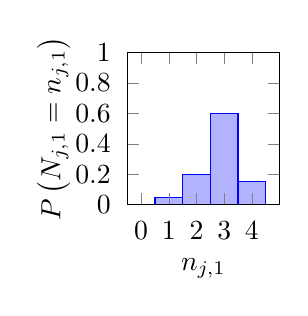
\begin{tikzpicture}
		\begin{axis}[
		width=100,
		height=100,
		domain=0:5,
		area style,
		xmin=-0.5,
		xmax=5,
		ymin=0,
		ymax=1,
		xtick={0,1,2,3,4},
		xticklabel style = {yshift=-0.25em},
		yticklabel style = {xshift=-0.25em},
		xlabel={$n_{j,1}$},
        ylabel={$P\left(N_{j,1} = n_{j,1}\right)$},
        ylabel style={yshift=-0.5em}
		%ylabel near ticks
		]
		\addplot+[ybar interval] plot coordinates {(0.5,0.05) (1.5,0.2) (2.5,0.6) (3.5,0.15) (4.5,0)};
		\end{axis}
		\end{tikzpicture}%
	};
	\node (s2) at (4, 1) {$n_{2,l}=2$}
		edge [<-] node [below right] {Sample} (D2);
	\node (s1) at (4, 3) {$n_{1,l}=3$}
		edge [<-] node [above right] {Sample} (D1);
	\node[draw, fit={(5,1.5) (6,2.5)}, inner sep=0pt, label=center:2, fill=black!20] (T1) {}
		edge [<-] (s1)
		edge [<-] (s2);
	\node[draw, fit={(6,1.5) (7,2.5)}, inner sep=0pt, label=center:1, fill=black!20] (T2) {};
	\node[draw, fit={(7,1.5) (8,2.5)}, inner sep=0pt, label=center:1, fill=black!20] (T3) {};
	\node[draw, fit={(8,1.5) (9,2.5)}, inner sep=0pt, label=center:2, fill=black!20] (T3) {};
	\node[draw, fit={(9,1.5) (10,2.5)}, inner sep=0pt, label=center:1, fill=black!20] (T3) {};
	\node (r) at (6.5, 2.8) {Random order:};
	\node (xl) at (8, 1) {$\boldsymbol{x}^k_{j,l} = [1, 2, 2, 1, M, 2]$};
	\draw [thick,
		decoration={
			brace,
			mirror,
		},
		decorate
		] (8.5, 2.8) -- (9.5,2.8);
	\node[draw, label={Insert maintenance{:}}, fit={(8.5,2.8) (9.5,3.8)}, inner sep=0pt, label=center:M, fill=black!30] (M) {};
	\node (calcp) at (8,-1) {Calculate $p^f_j(\boldsymbol{x}^k_{j,l})$}
		edge [<-] (xl);

	\draw[thick, dotted] (2.5,-1.5) rectangle (11, 4.5)
		node [above left] {Repeat $N$ times, $\bar{p}^f_j = \max p^f_j(\boldsymbol{x}^k_{j,l})${:} };

	\end{tikzpicture}
%\end{document}

}
\only<2>{
    % Created by tikzDevice version 0.11 on 2018-07-30 13:37:04
% !TEX encoding = UTF-8 Unicode
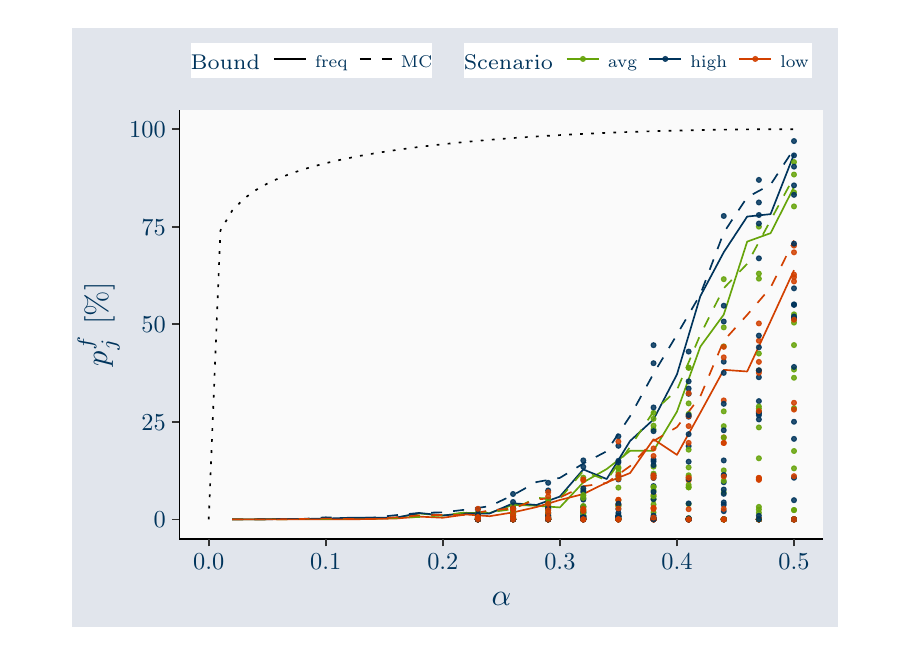
\begin{tikzpicture}[x=1pt,y=1pt]
\definecolor{fillColor}{RGB}{255,255,255}
\path[use as bounding box,fill=fillColor,fill opacity=0.00] (0,0) rectangle (308.59,216.81);
\begin{scope}
\path[clip] ( 15.61,  0.00) rectangle (292.98,216.81);
\definecolor{drawColor}{RGB}{255,255,255}
\definecolor{fillColor}{RGB}{225,229,236}

\path[draw=drawColor,line width= 0.6pt,line join=round,line cap=round,fill=fillColor] ( 15.61,  0.00) rectangle (292.98,216.81);
\end{scope}
\begin{scope}
\path[clip] ( 54.84, 32.09) rectangle (287.48,187.18);
\definecolor{fillColor}{gray}{0.98}

\path[fill=fillColor] ( 54.84, 32.09) rectangle (287.48,187.18);
\definecolor{drawColor}{RGB}{102,164,10}

\path[draw=drawColor,line width= 0.6pt,line join=round] ( 73.88, 39.14) --
	( 82.33, 39.14) --
	( 90.79, 39.28) --
	( 99.25, 39.28) --
	(107.71, 39.28) --
	(116.17, 39.31) --
	(124.63, 39.30) --
	(133.09, 39.70) --
	(141.55, 41.26) --
	(150.01, 40.50) --
	(158.47, 41.50) --
	(166.93, 41.40) --
	(175.39, 44.38) --
	(183.85, 44.05) --
	(192.31, 43.45) --
	(200.77, 52.51) --
	(209.23, 57.32) --
	(217.69, 63.91) --
	(226.15, 63.96) --
	(234.61, 78.05) --
	(243.07,101.56) --
	(251.53,113.13) --
	(259.99,139.50) --
	(268.45,142.55) --
	(276.91,159.22);
\definecolor{drawColor}{RGB}{0,52,92}

\path[draw=drawColor,line width= 0.6pt,line join=round] ( 73.88, 39.14) --
	( 82.33, 39.14) --
	( 90.79, 39.23) --
	( 99.25, 39.28) --
	(107.71, 39.42) --
	(116.17, 39.72) --
	(124.63, 39.72) --
	(133.09, 39.74) --
	(141.55, 41.44) --
	(150.01, 40.56) --
	(158.47, 41.31) --
	(166.93, 41.27) --
	(175.39, 44.94) --
	(183.85, 44.35) --
	(192.31, 47.37) --
	(200.77, 57.18) --
	(209.23, 53.71) --
	(217.69, 67.48) --
	(226.15, 75.25) --
	(234.61, 91.49) --
	(243.07,119.80) --
	(251.53,135.67) --
	(259.99,148.55) --
	(268.45,149.43) --
	(276.91,171.05);
\definecolor{drawColor}{RGB}{210,64,0}

\path[draw=drawColor,line width= 0.6pt,line join=round] ( 73.88, 39.14) --
	( 82.33, 39.14) --
	( 90.79, 39.14) --
	( 99.25, 39.14) --
	(107.71, 39.14) --
	(116.17, 39.14) --
	(124.63, 39.28) --
	(133.09, 39.44) --
	(141.55, 40.13) --
	(150.01, 39.72) --
	(158.47, 40.90) --
	(166.93, 40.28) --
	(175.39, 41.66) --
	(183.85, 43.57) --
	(192.31, 46.14) --
	(200.77, 48.28) --
	(209.23, 52.46) --
	(217.69, 55.89) --
	(226.15, 68.09) --
	(234.61, 62.44) --
	(243.07, 77.69) --
	(251.53, 93.17) --
	(259.99, 92.57) --
	(268.45,110.77) --
	(276.91,129.18);
\definecolor{drawColor}{RGB}{102,164,10}

\path[draw=drawColor,line width= 0.6pt,dash pattern=on 4pt off 4pt ,line join=round] ( 73.88, 39.14) --
	( 82.33, 39.14) --
	( 90.79, 39.14) --
	( 99.25, 39.28) --
	(107.71, 39.28) --
	(116.17, 39.28) --
	(124.63, 39.47) --
	(133.09, 39.62) --
	(141.55, 40.01) --
	(150.01, 40.56) --
	(158.47, 41.73) --
	(166.93, 41.71) --
	(175.39, 42.83) --
	(183.85, 46.87) --
	(192.31, 46.62) --
	(200.77, 56.61) --
	(209.23, 53.24) --
	(217.69, 65.34) --
	(226.15, 78.13) --
	(234.61, 85.88) --
	(243.07,105.89) --
	(251.53,122.66) --
	(259.99,131.48) --
	(268.45,147.20) --
	(276.91,162.88);
\definecolor{drawColor}{RGB}{0,52,92}

\path[draw=drawColor,line width= 0.6pt,dash pattern=on 4pt off 4pt ,line join=round] ( 73.88, 39.14) --
	( 82.33, 39.14) --
	( 90.79, 39.28) --
	( 99.25, 39.28) --
	(107.71, 39.88) --
	(116.17, 39.58) --
	(124.63, 39.74) --
	(133.09, 40.66) --
	(141.55, 41.45) --
	(150.01, 41.68) --
	(158.47, 42.67) --
	(166.93, 43.90) --
	(175.39, 47.90) --
	(183.85, 52.62) --
	(192.31, 54.12) --
	(200.77, 59.31) --
	(209.23, 63.74) --
	(217.69, 76.43) --
	(226.15, 91.79) --
	(234.61,105.87) --
	(243.07,120.42) --
	(251.53,142.79) --
	(259.99,155.53) --
	(268.45,160.09) --
	(276.91,173.03);
\definecolor{drawColor}{RGB}{210,64,0}

\path[draw=drawColor,line width= 0.6pt,dash pattern=on 4pt off 4pt ,line join=round] ( 73.88, 39.14) --
	( 82.33, 39.14) --
	( 90.79, 39.14) --
	( 99.25, 39.28) --
	(107.71, 39.42) --
	(116.17, 39.28) --
	(124.63, 39.28) --
	(133.09, 39.87) --
	(141.55, 40.58) --
	(150.01, 40.76) --
	(158.47, 40.65) --
	(166.93, 42.41) --
	(175.39, 43.08) --
	(183.85, 46.34) --
	(192.31, 47.02) --
	(200.77, 51.10) --
	(209.23, 52.31) --
	(217.69, 58.39) --
	(226.15, 67.45) --
	(234.61, 72.46) --
	(243.07, 83.60) --
	(251.53,103.70) --
	(259.99,113.03) --
	(268.45,122.88) --
	(276.91,139.89);
\definecolor{drawColor}{RGB}{102,164,10}
\definecolor{fillColor}{RGB}{102,164,10}

\path[draw=drawColor,draw opacity=0.85,line width= 0.4pt,line join=round,line cap=round,fill=fillColor,fill opacity=0.85] (162.70, 39.20) circle (  0.89);

\path[draw=drawColor,draw opacity=0.85,line width= 0.4pt,line join=round,line cap=round,fill=fillColor,fill opacity=0.85] (175.39, 39.14) circle (  0.89);

\path[draw=drawColor,draw opacity=0.85,line width= 0.4pt,line join=round,line cap=round,fill=fillColor,fill opacity=0.85] (188.08, 42.47) circle (  0.89);

\path[draw=drawColor,draw opacity=0.85,line width= 0.4pt,line join=round,line cap=round,fill=fillColor,fill opacity=0.85] (200.77, 43.49) circle (  0.89);

\path[draw=drawColor,draw opacity=0.85,line width= 0.4pt,line join=round,line cap=round,fill=fillColor,fill opacity=0.85] (213.46, 40.37) circle (  0.89);

\path[draw=drawColor,draw opacity=0.85,line width= 0.4pt,line join=round,line cap=round,fill=fillColor,fill opacity=0.85] (226.15, 44.52) circle (  0.89);

\path[draw=drawColor,draw opacity=0.85,line width= 0.4pt,line join=round,line cap=round,fill=fillColor,fill opacity=0.85] (238.84, 39.50) circle (  0.89);

\path[draw=drawColor,draw opacity=0.85,line width= 0.4pt,line join=round,line cap=round,fill=fillColor,fill opacity=0.85] (251.53, 56.84) circle (  0.89);

\path[draw=drawColor,draw opacity=0.85,line width= 0.4pt,line join=round,line cap=round,fill=fillColor,fill opacity=0.85] (264.22, 39.14) circle (  0.89);

\path[draw=drawColor,draw opacity=0.85,line width= 0.4pt,line join=round,line cap=round,fill=fillColor,fill opacity=0.85] (276.91, 42.51) circle (  0.89);

\path[draw=drawColor,draw opacity=0.85,line width= 0.4pt,line join=round,line cap=round,fill=fillColor,fill opacity=0.85] (162.70, 40.32) circle (  0.89);

\path[draw=drawColor,draw opacity=0.85,line width= 0.4pt,line join=round,line cap=round,fill=fillColor,fill opacity=0.85] (175.39, 44.16) circle (  0.89);

\path[draw=drawColor,draw opacity=0.85,line width= 0.4pt,line join=round,line cap=round,fill=fillColor,fill opacity=0.85] (188.08, 39.32) circle (  0.89);

\path[draw=drawColor,draw opacity=0.85,line width= 0.4pt,line join=round,line cap=round,fill=fillColor,fill opacity=0.85] (200.77, 43.72) circle (  0.89);

\path[draw=drawColor,draw opacity=0.85,line width= 0.4pt,line join=round,line cap=round,fill=fillColor,fill opacity=0.85] (213.46, 39.14) circle (  0.89);

\path[draw=drawColor,draw opacity=0.85,line width= 0.4pt,line join=round,line cap=round,fill=fillColor,fill opacity=0.85] (226.15, 55.66) circle (  0.89);

\path[draw=drawColor,draw opacity=0.85,line width= 0.4pt,line join=round,line cap=round,fill=fillColor,fill opacity=0.85] (238.84, 39.54) circle (  0.89);

\path[draw=drawColor,draw opacity=0.85,line width= 0.4pt,line join=round,line cap=round,fill=fillColor,fill opacity=0.85] (251.53, 39.14) circle (  0.89);

\path[draw=drawColor,draw opacity=0.85,line width= 0.4pt,line join=round,line cap=round,fill=fillColor,fill opacity=0.85] (264.22, 39.14) circle (  0.89);

\path[draw=drawColor,draw opacity=0.85,line width= 0.4pt,line join=round,line cap=round,fill=fillColor,fill opacity=0.85] (276.91, 57.57) circle (  0.89);

\path[draw=drawColor,draw opacity=0.85,line width= 0.4pt,line join=round,line cap=round,fill=fillColor,fill opacity=0.85] (162.70, 39.52) circle (  0.89);

\path[draw=drawColor,draw opacity=0.85,line width= 0.4pt,line join=round,line cap=round,fill=fillColor,fill opacity=0.85] (175.39, 39.14) circle (  0.89);

\path[draw=drawColor,draw opacity=0.85,line width= 0.4pt,line join=round,line cap=round,fill=fillColor,fill opacity=0.85] (188.08, 40.52) circle (  0.89);

\path[draw=drawColor,draw opacity=0.85,line width= 0.4pt,line join=round,line cap=round,fill=fillColor,fill opacity=0.85] (200.77, 47.62) circle (  0.89);

\path[draw=drawColor,draw opacity=0.85,line width= 0.4pt,line join=round,line cap=round,fill=fillColor,fill opacity=0.85] (213.46, 39.24) circle (  0.89);

\path[draw=drawColor,draw opacity=0.85,line width= 0.4pt,line join=round,line cap=round,fill=fillColor,fill opacity=0.85] (226.15, 39.14) circle (  0.89);

\path[draw=drawColor,draw opacity=0.85,line width= 0.4pt,line join=round,line cap=round,fill=fillColor,fill opacity=0.85] (238.84, 39.14) circle (  0.89);

\path[draw=drawColor,draw opacity=0.85,line width= 0.4pt,line join=round,line cap=round,fill=fillColor,fill opacity=0.85] (251.53, 39.14) circle (  0.89);

\path[draw=drawColor,draw opacity=0.85,line width= 0.4pt,line join=round,line cap=round,fill=fillColor,fill opacity=0.85] (264.22, 72.36) circle (  0.89);

\path[draw=drawColor,draw opacity=0.85,line width= 0.4pt,line join=round,line cap=round,fill=fillColor,fill opacity=0.85] (276.91, 42.48) circle (  0.89);

\path[draw=drawColor,draw opacity=0.85,line width= 0.4pt,line join=round,line cap=round,fill=fillColor,fill opacity=0.85] (162.70, 40.77) circle (  0.89);

\path[draw=drawColor,draw opacity=0.85,line width= 0.4pt,line join=round,line cap=round,fill=fillColor,fill opacity=0.85] (175.39, 39.14) circle (  0.89);

\path[draw=drawColor,draw opacity=0.85,line width= 0.4pt,line join=round,line cap=round,fill=fillColor,fill opacity=0.85] (188.08, 39.14) circle (  0.89);

\path[draw=drawColor,draw opacity=0.85,line width= 0.4pt,line join=round,line cap=round,fill=fillColor,fill opacity=0.85] (200.77, 40.09) circle (  0.89);

\path[draw=drawColor,draw opacity=0.85,line width= 0.4pt,line join=round,line cap=round,fill=fillColor,fill opacity=0.85] (213.46, 39.14) circle (  0.89);

\path[draw=drawColor,draw opacity=0.85,line width= 0.4pt,line join=round,line cap=round,fill=fillColor,fill opacity=0.85] (226.15, 39.47) circle (  0.89);

\path[draw=drawColor,draw opacity=0.85,line width= 0.4pt,line join=round,line cap=round,fill=fillColor,fill opacity=0.85] (238.84, 39.14) circle (  0.89);

\path[draw=drawColor,draw opacity=0.85,line width= 0.4pt,line join=round,line cap=round,fill=fillColor,fill opacity=0.85] (251.53, 72.81) circle (  0.89);

\path[draw=drawColor,draw opacity=0.85,line width= 0.4pt,line join=round,line cap=round,fill=fillColor,fill opacity=0.85] (264.22, 92.92) circle (  0.89);

\path[draw=drawColor,draw opacity=0.85,line width= 0.4pt,line join=round,line cap=round,fill=fillColor,fill opacity=0.85] (276.91, 39.14) circle (  0.89);
\definecolor{drawColor}{RGB}{0,52,92}
\definecolor{fillColor}{RGB}{0,52,92}

\path[draw=drawColor,draw opacity=0.85,line width= 0.4pt,line join=round,line cap=round,fill=fillColor,fill opacity=0.85] (162.70, 41.20) circle (  0.89);

\path[draw=drawColor,draw opacity=0.85,line width= 0.4pt,line join=round,line cap=round,fill=fillColor,fill opacity=0.85] (175.39, 39.14) circle (  0.89);

\path[draw=drawColor,draw opacity=0.85,line width= 0.4pt,line join=round,line cap=round,fill=fillColor,fill opacity=0.85] (188.08, 45.40) circle (  0.89);

\path[draw=drawColor,draw opacity=0.85,line width= 0.4pt,line join=round,line cap=round,fill=fillColor,fill opacity=0.85] (200.77, 46.28) circle (  0.89);

\path[draw=drawColor,draw opacity=0.85,line width= 0.4pt,line join=round,line cap=round,fill=fillColor,fill opacity=0.85] (213.46, 39.14) circle (  0.89);

\path[draw=drawColor,draw opacity=0.85,line width= 0.4pt,line join=round,line cap=round,fill=fillColor,fill opacity=0.85] (226.15, 39.61) circle (  0.89);

\path[draw=drawColor,draw opacity=0.85,line width= 0.4pt,line join=round,line cap=round,fill=fillColor,fill opacity=0.85] (238.84, 39.14) circle (  0.89);

\path[draw=drawColor,draw opacity=0.85,line width= 0.4pt,line join=round,line cap=round,fill=fillColor,fill opacity=0.85] (251.53, 39.14) circle (  0.89);

\path[draw=drawColor,draw opacity=0.85,line width= 0.4pt,line join=round,line cap=round,fill=fillColor,fill opacity=0.85] (264.22, 39.14) circle (  0.89);

\path[draw=drawColor,draw opacity=0.85,line width= 0.4pt,line join=round,line cap=round,fill=fillColor,fill opacity=0.85] (276.91,111.47) circle (  0.89);

\path[draw=drawColor,draw opacity=0.85,line width= 0.4pt,line join=round,line cap=round,fill=fillColor,fill opacity=0.85] (162.70, 39.14) circle (  0.89);

\path[draw=drawColor,draw opacity=0.85,line width= 0.4pt,line join=round,line cap=round,fill=fillColor,fill opacity=0.85] (175.39, 39.14) circle (  0.89);

\path[draw=drawColor,draw opacity=0.85,line width= 0.4pt,line join=round,line cap=round,fill=fillColor,fill opacity=0.85] (188.08, 43.98) circle (  0.89);

\path[draw=drawColor,draw opacity=0.85,line width= 0.4pt,line join=round,line cap=round,fill=fillColor,fill opacity=0.85] (200.77, 39.14) circle (  0.89);

\path[draw=drawColor,draw opacity=0.85,line width= 0.4pt,line join=round,line cap=round,fill=fillColor,fill opacity=0.85] (213.46, 39.14) circle (  0.89);

\path[draw=drawColor,draw opacity=0.85,line width= 0.4pt,line join=round,line cap=round,fill=fillColor,fill opacity=0.85] (226.15, 39.14) circle (  0.89);

\path[draw=drawColor,draw opacity=0.85,line width= 0.4pt,line join=round,line cap=round,fill=fillColor,fill opacity=0.85] (238.84, 39.14) circle (  0.89);

\path[draw=drawColor,draw opacity=0.85,line width= 0.4pt,line join=round,line cap=round,fill=fillColor,fill opacity=0.85] (251.53, 71.33) circle (  0.89);

\path[draw=drawColor,draw opacity=0.85,line width= 0.4pt,line join=round,line cap=round,fill=fillColor,fill opacity=0.85] (264.22, 39.14) circle (  0.89);

\path[draw=drawColor,draw opacity=0.85,line width= 0.4pt,line join=round,line cap=round,fill=fillColor,fill opacity=0.85] (276.91,116.63) circle (  0.89);

\path[draw=drawColor,draw opacity=0.85,line width= 0.4pt,line join=round,line cap=round,fill=fillColor,fill opacity=0.85] (162.70, 39.14) circle (  0.89);

\path[draw=drawColor,draw opacity=0.85,line width= 0.4pt,line join=round,line cap=round,fill=fillColor,fill opacity=0.85] (175.39, 39.14) circle (  0.89);

\path[draw=drawColor,draw opacity=0.85,line width= 0.4pt,line join=round,line cap=round,fill=fillColor,fill opacity=0.85] (188.08, 39.14) circle (  0.89);

\path[draw=drawColor,draw opacity=0.85,line width= 0.4pt,line join=round,line cap=round,fill=fillColor,fill opacity=0.85] (200.77, 39.14) circle (  0.89);

\path[draw=drawColor,draw opacity=0.85,line width= 0.4pt,line join=round,line cap=round,fill=fillColor,fill opacity=0.85] (213.46, 39.14) circle (  0.89);

\path[draw=drawColor,draw opacity=0.85,line width= 0.4pt,line join=round,line cap=round,fill=fillColor,fill opacity=0.85] (226.15, 54.09) circle (  0.89);

\path[draw=drawColor,draw opacity=0.85,line width= 0.4pt,line join=round,line cap=round,fill=fillColor,fill opacity=0.85] (238.84, 39.14) circle (  0.89);

\path[draw=drawColor,draw opacity=0.85,line width= 0.4pt,line join=round,line cap=round,fill=fillColor,fill opacity=0.85] (251.53, 39.14) circle (  0.89);

\path[draw=drawColor,draw opacity=0.85,line width= 0.4pt,line join=round,line cap=round,fill=fillColor,fill opacity=0.85] (264.22, 39.14) circle (  0.89);

\path[draw=drawColor,draw opacity=0.85,line width= 0.4pt,line join=round,line cap=round,fill=fillColor,fill opacity=0.85] (276.91, 39.14) circle (  0.89);

\path[draw=drawColor,draw opacity=0.85,line width= 0.4pt,line join=round,line cap=round,fill=fillColor,fill opacity=0.85] (162.70, 39.14) circle (  0.89);

\path[draw=drawColor,draw opacity=0.85,line width= 0.4pt,line join=round,line cap=round,fill=fillColor,fill opacity=0.85] (175.39, 39.14) circle (  0.89);

\path[draw=drawColor,draw opacity=0.85,line width= 0.4pt,line join=round,line cap=round,fill=fillColor,fill opacity=0.85] (188.08, 45.13) circle (  0.89);

\path[draw=drawColor,draw opacity=0.85,line width= 0.4pt,line join=round,line cap=round,fill=fillColor,fill opacity=0.85] (200.77, 43.72) circle (  0.89);

\path[draw=drawColor,draw opacity=0.85,line width= 0.4pt,line join=round,line cap=round,fill=fillColor,fill opacity=0.85] (213.46, 44.39) circle (  0.89);

\path[draw=drawColor,draw opacity=0.85,line width= 0.4pt,line join=round,line cap=round,fill=fillColor,fill opacity=0.85] (226.15, 39.14) circle (  0.89);

\path[draw=drawColor,draw opacity=0.85,line width= 0.4pt,line join=round,line cap=round,fill=fillColor,fill opacity=0.85] (238.84, 65.60) circle (  0.89);

\path[draw=drawColor,draw opacity=0.85,line width= 0.4pt,line join=round,line cap=round,fill=fillColor,fill opacity=0.85] (251.53, 55.18) circle (  0.89);

\path[draw=drawColor,draw opacity=0.85,line width= 0.4pt,line join=round,line cap=round,fill=fillColor,fill opacity=0.85] (264.22, 90.49) circle (  0.89);

\path[draw=drawColor,draw opacity=0.85,line width= 0.4pt,line join=round,line cap=round,fill=fillColor,fill opacity=0.85] (276.91,112.06) circle (  0.89);

\path[draw=drawColor,draw opacity=0.85,line width= 0.4pt,line join=round,line cap=round,fill=fillColor,fill opacity=0.85] (162.70, 39.14) circle (  0.89);

\path[draw=drawColor,draw opacity=0.85,line width= 0.4pt,line join=round,line cap=round,fill=fillColor,fill opacity=0.85] (175.39, 39.14) circle (  0.89);

\path[draw=drawColor,draw opacity=0.85,line width= 0.4pt,line join=round,line cap=round,fill=fillColor,fill opacity=0.85] (188.08, 39.14) circle (  0.89);

\path[draw=drawColor,draw opacity=0.85,line width= 0.4pt,line join=round,line cap=round,fill=fillColor,fill opacity=0.85] (200.77, 39.14) circle (  0.89);

\path[draw=drawColor,draw opacity=0.85,line width= 0.4pt,line join=round,line cap=round,fill=fillColor,fill opacity=0.85] (213.46, 54.74) circle (  0.89);

\path[draw=drawColor,draw opacity=0.85,line width= 0.4pt,line join=round,line cap=round,fill=fillColor,fill opacity=0.85] (226.15, 39.14) circle (  0.89);

\path[draw=drawColor,draw opacity=0.85,line width= 0.4pt,line join=round,line cap=round,fill=fillColor,fill opacity=0.85] (238.84, 39.14) circle (  0.89);

\path[draw=drawColor,draw opacity=0.85,line width= 0.4pt,line join=round,line cap=round,fill=fillColor,fill opacity=0.85] (251.53, 39.14) circle (  0.89);

\path[draw=drawColor,draw opacity=0.85,line width= 0.4pt,line join=round,line cap=round,fill=fillColor,fill opacity=0.85] (264.22, 39.14) circle (  0.89);

\path[draw=drawColor,draw opacity=0.85,line width= 0.4pt,line join=round,line cap=round,fill=fillColor,fill opacity=0.85] (276.91, 39.14) circle (  0.89);
\definecolor{drawColor}{RGB}{210,64,0}
\definecolor{fillColor}{RGB}{210,64,0}

\path[draw=drawColor,draw opacity=0.85,line width= 0.4pt,line join=round,line cap=round,fill=fillColor,fill opacity=0.85] (162.70, 39.14) circle (  0.89);

\path[draw=drawColor,draw opacity=0.85,line width= 0.4pt,line join=round,line cap=round,fill=fillColor,fill opacity=0.85] (175.39, 39.14) circle (  0.89);

\path[draw=drawColor,draw opacity=0.85,line width= 0.4pt,line join=round,line cap=round,fill=fillColor,fill opacity=0.85] (188.08, 39.14) circle (  0.89);

\path[draw=drawColor,draw opacity=0.85,line width= 0.4pt,line join=round,line cap=round,fill=fillColor,fill opacity=0.85] (200.77, 39.14) circle (  0.89);

\path[draw=drawColor,draw opacity=0.85,line width= 0.4pt,line join=round,line cap=round,fill=fillColor,fill opacity=0.85] (213.46, 39.14) circle (  0.89);

\path[draw=drawColor,draw opacity=0.85,line width= 0.4pt,line join=round,line cap=round,fill=fillColor,fill opacity=0.85] (226.15, 39.14) circle (  0.89);

\path[draw=drawColor,draw opacity=0.85,line width= 0.4pt,line join=round,line cap=round,fill=fillColor,fill opacity=0.85] (238.84, 39.14) circle (  0.89);

\path[draw=drawColor,draw opacity=0.85,line width= 0.4pt,line join=round,line cap=round,fill=fillColor,fill opacity=0.85] (251.53, 39.14) circle (  0.89);

\path[draw=drawColor,draw opacity=0.85,line width= 0.4pt,line join=round,line cap=round,fill=fillColor,fill opacity=0.85] (264.22, 39.14) circle (  0.89);

\path[draw=drawColor,draw opacity=0.85,line width= 0.4pt,line join=round,line cap=round,fill=fillColor,fill opacity=0.85] (276.91, 39.14) circle (  0.89);

\path[draw=drawColor,draw opacity=0.85,line width= 0.4pt,line join=round,line cap=round,fill=fillColor,fill opacity=0.85] (162.70, 39.14) circle (  0.89);

\path[draw=drawColor,draw opacity=0.85,line width= 0.4pt,line join=round,line cap=round,fill=fillColor,fill opacity=0.85] (175.39, 39.14) circle (  0.89);

\path[draw=drawColor,draw opacity=0.85,line width= 0.4pt,line join=round,line cap=round,fill=fillColor,fill opacity=0.85] (188.08, 39.14) circle (  0.89);

\path[draw=drawColor,draw opacity=0.85,line width= 0.4pt,line join=round,line cap=round,fill=fillColor,fill opacity=0.85] (200.77, 39.14) circle (  0.89);

\path[draw=drawColor,draw opacity=0.85,line width= 0.4pt,line join=round,line cap=round,fill=fillColor,fill opacity=0.85] (213.46, 39.14) circle (  0.89);

\path[draw=drawColor,draw opacity=0.85,line width= 0.4pt,line join=round,line cap=round,fill=fillColor,fill opacity=0.85] (226.15, 39.14) circle (  0.89);

\path[draw=drawColor,draw opacity=0.85,line width= 0.4pt,line join=round,line cap=round,fill=fillColor,fill opacity=0.85] (238.84, 39.14) circle (  0.89);

\path[draw=drawColor,draw opacity=0.85,line width= 0.4pt,line join=round,line cap=round,fill=fillColor,fill opacity=0.85] (251.53, 39.14) circle (  0.89);

\path[draw=drawColor,draw opacity=0.85,line width= 0.4pt,line join=round,line cap=round,fill=fillColor,fill opacity=0.85] (264.22, 39.14) circle (  0.89);

\path[draw=drawColor,draw opacity=0.85,line width= 0.4pt,line join=round,line cap=round,fill=fillColor,fill opacity=0.85] (276.91, 39.14) circle (  0.89);

\path[draw=drawColor,draw opacity=0.85,line width= 0.4pt,line join=round,line cap=round,fill=fillColor,fill opacity=0.85] (162.70, 39.14) circle (  0.89);

\path[draw=drawColor,draw opacity=0.85,line width= 0.4pt,line join=round,line cap=round,fill=fillColor,fill opacity=0.85] (175.39, 39.14) circle (  0.89);

\path[draw=drawColor,draw opacity=0.85,line width= 0.4pt,line join=round,line cap=round,fill=fillColor,fill opacity=0.85] (188.08, 39.14) circle (  0.89);

\path[draw=drawColor,draw opacity=0.85,line width= 0.4pt,line join=round,line cap=round,fill=fillColor,fill opacity=0.85] (200.77, 39.14) circle (  0.89);

\path[draw=drawColor,draw opacity=0.85,line width= 0.4pt,line join=round,line cap=round,fill=fillColor,fill opacity=0.85] (213.46, 39.14) circle (  0.89);

\path[draw=drawColor,draw opacity=0.85,line width= 0.4pt,line join=round,line cap=round,fill=fillColor,fill opacity=0.85] (226.15, 39.14) circle (  0.89);

\path[draw=drawColor,draw opacity=0.85,line width= 0.4pt,line join=round,line cap=round,fill=fillColor,fill opacity=0.85] (238.84, 39.14) circle (  0.89);

\path[draw=drawColor,draw opacity=0.85,line width= 0.4pt,line join=round,line cap=round,fill=fillColor,fill opacity=0.85] (251.53, 39.14) circle (  0.89);

\path[draw=drawColor,draw opacity=0.85,line width= 0.4pt,line join=round,line cap=round,fill=fillColor,fill opacity=0.85] (264.22, 39.14) circle (  0.89);

\path[draw=drawColor,draw opacity=0.85,line width= 0.4pt,line join=round,line cap=round,fill=fillColor,fill opacity=0.85] (276.91, 39.14) circle (  0.89);

\path[draw=drawColor,draw opacity=0.85,line width= 0.4pt,line join=round,line cap=round,fill=fillColor,fill opacity=0.85] (162.70, 39.14) circle (  0.89);

\path[draw=drawColor,draw opacity=0.85,line width= 0.4pt,line join=round,line cap=round,fill=fillColor,fill opacity=0.85] (175.39, 39.14) circle (  0.89);

\path[draw=drawColor,draw opacity=0.85,line width= 0.4pt,line join=round,line cap=round,fill=fillColor,fill opacity=0.85] (188.08, 39.14) circle (  0.89);

\path[draw=drawColor,draw opacity=0.85,line width= 0.4pt,line join=round,line cap=round,fill=fillColor,fill opacity=0.85] (200.77, 39.14) circle (  0.89);

\path[draw=drawColor,draw opacity=0.85,line width= 0.4pt,line join=round,line cap=round,fill=fillColor,fill opacity=0.85] (213.46, 39.14) circle (  0.89);

\path[draw=drawColor,draw opacity=0.85,line width= 0.4pt,line join=round,line cap=round,fill=fillColor,fill opacity=0.85] (226.15, 39.14) circle (  0.89);

\path[draw=drawColor,draw opacity=0.85,line width= 0.4pt,line join=round,line cap=round,fill=fillColor,fill opacity=0.85] (238.84, 39.14) circle (  0.89);

\path[draw=drawColor,draw opacity=0.85,line width= 0.4pt,line join=round,line cap=round,fill=fillColor,fill opacity=0.85] (251.53, 39.14) circle (  0.89);

\path[draw=drawColor,draw opacity=0.85,line width= 0.4pt,line join=round,line cap=round,fill=fillColor,fill opacity=0.85] (264.22, 39.14) circle (  0.89);

\path[draw=drawColor,draw opacity=0.85,line width= 0.4pt,line join=round,line cap=round,fill=fillColor,fill opacity=0.85] (276.91, 39.14) circle (  0.89);

\path[draw=drawColor,draw opacity=0.85,line width= 0.4pt,line join=round,line cap=round,fill=fillColor,fill opacity=0.85] (162.70, 39.14) circle (  0.89);

\path[draw=drawColor,draw opacity=0.85,line width= 0.4pt,line join=round,line cap=round,fill=fillColor,fill opacity=0.85] (175.39, 39.14) circle (  0.89);

\path[draw=drawColor,draw opacity=0.85,line width= 0.4pt,line join=round,line cap=round,fill=fillColor,fill opacity=0.85] (188.08, 39.14) circle (  0.89);

\path[draw=drawColor,draw opacity=0.85,line width= 0.4pt,line join=round,line cap=round,fill=fillColor,fill opacity=0.85] (200.77, 39.14) circle (  0.89);

\path[draw=drawColor,draw opacity=0.85,line width= 0.4pt,line join=round,line cap=round,fill=fillColor,fill opacity=0.85] (213.46, 39.14) circle (  0.89);

\path[draw=drawColor,draw opacity=0.85,line width= 0.4pt,line join=round,line cap=round,fill=fillColor,fill opacity=0.85] (226.15, 39.14) circle (  0.89);

\path[draw=drawColor,draw opacity=0.85,line width= 0.4pt,line join=round,line cap=round,fill=fillColor,fill opacity=0.85] (238.84, 39.14) circle (  0.89);

\path[draw=drawColor,draw opacity=0.85,line width= 0.4pt,line join=round,line cap=round,fill=fillColor,fill opacity=0.85] (251.53, 39.14) circle (  0.89);

\path[draw=drawColor,draw opacity=0.85,line width= 0.4pt,line join=round,line cap=round,fill=fillColor,fill opacity=0.85] (264.22, 39.14) circle (  0.89);

\path[draw=drawColor,draw opacity=0.85,line width= 0.4pt,line join=round,line cap=round,fill=fillColor,fill opacity=0.85] (276.91, 39.14) circle (  0.89);
\definecolor{drawColor}{RGB}{102,164,10}
\definecolor{fillColor}{RGB}{102,164,10}

\path[draw=drawColor,draw opacity=0.85,line width= 0.4pt,line join=round,line cap=round,fill=fillColor,fill opacity=0.85] (162.70, 41.34) circle (  0.89);

\path[draw=drawColor,draw opacity=0.85,line width= 0.4pt,line join=round,line cap=round,fill=fillColor,fill opacity=0.85] (175.39, 40.64) circle (  0.89);

\path[draw=drawColor,draw opacity=0.85,line width= 0.4pt,line join=round,line cap=round,fill=fillColor,fill opacity=0.85] (188.08, 45.02) circle (  0.89);

\path[draw=drawColor,draw opacity=0.85,line width= 0.4pt,line join=round,line cap=round,fill=fillColor,fill opacity=0.85] (200.77, 54.23) circle (  0.89);

\path[draw=drawColor,draw opacity=0.85,line width= 0.4pt,line join=round,line cap=round,fill=fillColor,fill opacity=0.85] (213.46, 45.97) circle (  0.89);

\path[draw=drawColor,draw opacity=0.85,line width= 0.4pt,line join=round,line cap=round,fill=fillColor,fill opacity=0.85] (226.15, 77.63) circle (  0.89);

\path[draw=drawColor,draw opacity=0.85,line width= 0.4pt,line join=round,line cap=round,fill=fillColor,fill opacity=0.85] (238.84, 81.04) circle (  0.89);

\path[draw=drawColor,draw opacity=0.85,line width= 0.4pt,line join=round,line cap=round,fill=fillColor,fill opacity=0.85] (251.53, 78.17) circle (  0.89);

\path[draw=drawColor,draw opacity=0.85,line width= 0.4pt,line join=round,line cap=round,fill=fillColor,fill opacity=0.85] (264.22, 99.06) circle (  0.89);

\path[draw=drawColor,draw opacity=0.85,line width= 0.4pt,line join=round,line cap=round,fill=fillColor,fill opacity=0.85] (276.91,157.30) circle (  0.89);

\path[draw=drawColor,draw opacity=0.85,line width= 0.4pt,line join=round,line cap=round,fill=fillColor,fill opacity=0.85] (162.70, 39.23) circle (  0.89);

\path[draw=drawColor,draw opacity=0.85,line width= 0.4pt,line join=round,line cap=round,fill=fillColor,fill opacity=0.85] (175.39, 41.22) circle (  0.89);

\path[draw=drawColor,draw opacity=0.85,line width= 0.4pt,line join=round,line cap=round,fill=fillColor,fill opacity=0.85] (188.08, 43.10) circle (  0.89);

\path[draw=drawColor,draw opacity=0.85,line width= 0.4pt,line join=round,line cap=round,fill=fillColor,fill opacity=0.85] (200.77, 42.60) circle (  0.89);

\path[draw=drawColor,draw opacity=0.85,line width= 0.4pt,line join=round,line cap=round,fill=fillColor,fill opacity=0.85] (213.46, 57.57) circle (  0.89);

\path[draw=drawColor,draw opacity=0.85,line width= 0.4pt,line join=round,line cap=round,fill=fillColor,fill opacity=0.85] (226.15, 72.99) circle (  0.89);

\path[draw=drawColor,draw opacity=0.85,line width= 0.4pt,line join=round,line cap=round,fill=fillColor,fill opacity=0.85] (238.84, 93.98) circle (  0.89);

\path[draw=drawColor,draw opacity=0.85,line width= 0.4pt,line join=round,line cap=round,fill=fillColor,fill opacity=0.85] (251.53,125.93) circle (  0.89);

\path[draw=drawColor,draw opacity=0.85,line width= 0.4pt,line join=round,line cap=round,fill=fillColor,fill opacity=0.85] (264.22,126.11) circle (  0.89);

\path[draw=drawColor,draw opacity=0.85,line width= 0.4pt,line join=round,line cap=round,fill=fillColor,fill opacity=0.85] (276.91,163.74) circle (  0.89);

\path[draw=drawColor,draw opacity=0.85,line width= 0.4pt,line join=round,line cap=round,fill=fillColor,fill opacity=0.85] (162.70, 40.95) circle (  0.89);

\path[draw=drawColor,draw opacity=0.85,line width= 0.4pt,line join=round,line cap=round,fill=fillColor,fill opacity=0.85] (175.39, 42.82) circle (  0.89);

\path[draw=drawColor,draw opacity=0.85,line width= 0.4pt,line join=round,line cap=round,fill=fillColor,fill opacity=0.85] (188.08, 44.28) circle (  0.89);

\path[draw=drawColor,draw opacity=0.85,line width= 0.4pt,line join=round,line cap=round,fill=fillColor,fill opacity=0.85] (200.77, 42.10) circle (  0.89);

\path[draw=drawColor,draw opacity=0.85,line width= 0.4pt,line join=round,line cap=round,fill=fillColor,fill opacity=0.85] (213.46, 44.14) circle (  0.89);

\path[draw=drawColor,draw opacity=0.85,line width= 0.4pt,line join=round,line cap=round,fill=fillColor,fill opacity=0.85] (226.15, 75.48) circle (  0.89);

\path[draw=drawColor,draw opacity=0.85,line width= 0.4pt,line join=round,line cap=round,fill=fillColor,fill opacity=0.85] (238.84, 77.24) circle (  0.89);

\path[draw=drawColor,draw opacity=0.85,line width= 0.4pt,line join=round,line cap=round,fill=fillColor,fill opacity=0.85] (251.53,108.51) circle (  0.89);

\path[draw=drawColor,draw opacity=0.85,line width= 0.4pt,line join=round,line cap=round,fill=fillColor,fill opacity=0.85] (264.22,127.94) circle (  0.89);

\path[draw=drawColor,draw opacity=0.85,line width= 0.4pt,line join=round,line cap=round,fill=fillColor,fill opacity=0.85] (276.91,152.22) circle (  0.89);

\path[draw=drawColor,draw opacity=0.85,line width= 0.4pt,line join=round,line cap=round,fill=fillColor,fill opacity=0.85] (162.70, 39.31) circle (  0.89);

\path[draw=drawColor,draw opacity=0.85,line width= 0.4pt,line join=round,line cap=round,fill=fillColor,fill opacity=0.85] (175.39, 40.51) circle (  0.89);

\path[draw=drawColor,draw opacity=0.85,line width= 0.4pt,line join=round,line cap=round,fill=fillColor,fill opacity=0.85] (188.08, 46.31) circle (  0.89);

\path[draw=drawColor,draw opacity=0.85,line width= 0.4pt,line join=round,line cap=round,fill=fillColor,fill opacity=0.85] (200.77, 49.63) circle (  0.89);

\path[draw=drawColor,draw opacity=0.85,line width= 0.4pt,line join=round,line cap=round,fill=fillColor,fill opacity=0.85] (213.46, 57.95) circle (  0.89);

\path[draw=drawColor,draw opacity=0.85,line width= 0.4pt,line join=round,line cap=round,fill=fillColor,fill opacity=0.85] (226.15, 71.64) circle (  0.89);

\path[draw=drawColor,draw opacity=0.85,line width= 0.4pt,line join=round,line cap=round,fill=fillColor,fill opacity=0.85] (238.84, 93.89) circle (  0.89);

\path[draw=drawColor,draw opacity=0.85,line width= 0.4pt,line join=round,line cap=round,fill=fillColor,fill opacity=0.85] (251.53,101.64) circle (  0.89);

\path[draw=drawColor,draw opacity=0.85,line width= 0.4pt,line join=round,line cap=round,fill=fillColor,fill opacity=0.85] (264.22,144.90) circle (  0.89);

\path[draw=drawColor,draw opacity=0.85,line width= 0.4pt,line join=round,line cap=round,fill=fillColor,fill opacity=0.85] (276.91,168.25) circle (  0.89);
\definecolor{drawColor}{RGB}{0,52,92}
\definecolor{fillColor}{RGB}{0,52,92}

\path[draw=drawColor,draw opacity=0.85,line width= 0.4pt,line join=round,line cap=round,fill=fillColor,fill opacity=0.85] (162.70, 39.38) circle (  0.89);

\path[draw=drawColor,draw opacity=0.85,line width= 0.4pt,line join=round,line cap=round,fill=fillColor,fill opacity=0.85] (175.39, 41.95) circle (  0.89);

\path[draw=drawColor,draw opacity=0.85,line width= 0.4pt,line join=round,line cap=round,fill=fillColor,fill opacity=0.85] (188.08, 49.58) circle (  0.89);

\path[draw=drawColor,draw opacity=0.85,line width= 0.4pt,line join=round,line cap=round,fill=fillColor,fill opacity=0.85] (200.77, 49.07) circle (  0.89);

\path[draw=drawColor,draw opacity=0.85,line width= 0.4pt,line join=round,line cap=round,fill=fillColor,fill opacity=0.85] (213.46, 65.72) circle (  0.89);

\path[draw=drawColor,draw opacity=0.85,line width= 0.4pt,line join=round,line cap=round,fill=fillColor,fill opacity=0.85] (226.15, 95.56) circle (  0.89);

\path[draw=drawColor,draw opacity=0.85,line width= 0.4pt,line join=round,line cap=round,fill=fillColor,fill opacity=0.85] (238.84, 89.01) circle (  0.89);

\path[draw=drawColor,draw opacity=0.85,line width= 0.4pt,line join=round,line cap=round,fill=fillColor,fill opacity=0.85] (251.53, 96.12) circle (  0.89);

\path[draw=drawColor,draw opacity=0.85,line width= 0.4pt,line join=round,line cap=round,fill=fillColor,fill opacity=0.85] (264.22,146.03) circle (  0.89);

\path[draw=drawColor,draw opacity=0.85,line width= 0.4pt,line join=round,line cap=round,fill=fillColor,fill opacity=0.85] (276.91,175.83) circle (  0.89);

\path[draw=drawColor,draw opacity=0.85,line width= 0.4pt,line join=round,line cap=round,fill=fillColor,fill opacity=0.85] (162.70, 41.00) circle (  0.89);

\path[draw=drawColor,draw opacity=0.85,line width= 0.4pt,line join=round,line cap=round,fill=fillColor,fill opacity=0.85] (175.39, 42.21) circle (  0.89);

\path[draw=drawColor,draw opacity=0.85,line width= 0.4pt,line join=round,line cap=round,fill=fillColor,fill opacity=0.85] (188.08, 52.35) circle (  0.89);

\path[draw=drawColor,draw opacity=0.85,line width= 0.4pt,line join=round,line cap=round,fill=fillColor,fill opacity=0.85] (200.77, 46.75) circle (  0.89);

\path[draw=drawColor,draw opacity=0.85,line width= 0.4pt,line join=round,line cap=round,fill=fillColor,fill opacity=0.85] (213.46, 60.28) circle (  0.89);

\path[draw=drawColor,draw opacity=0.85,line width= 0.4pt,line join=round,line cap=round,fill=fillColor,fill opacity=0.85] (226.15,102.08) circle (  0.89);

\path[draw=drawColor,draw opacity=0.85,line width= 0.4pt,line join=round,line cap=round,fill=fillColor,fill opacity=0.85] (238.84, 84.51) circle (  0.89);

\path[draw=drawColor,draw opacity=0.85,line width= 0.4pt,line join=round,line cap=round,fill=fillColor,fill opacity=0.85] (251.53, 92.08) circle (  0.89);

\path[draw=drawColor,draw opacity=0.85,line width= 0.4pt,line join=round,line cap=round,fill=fillColor,fill opacity=0.85] (264.22,149.12) circle (  0.89);

\path[draw=drawColor,draw opacity=0.85,line width= 0.4pt,line join=round,line cap=round,fill=fillColor,fill opacity=0.85] (276.91,170.66) circle (  0.89);

\path[draw=drawColor,draw opacity=0.85,line width= 0.4pt,line join=round,line cap=round,fill=fillColor,fill opacity=0.85] (162.70, 42.80) circle (  0.89);

\path[draw=drawColor,draw opacity=0.85,line width= 0.4pt,line join=round,line cap=round,fill=fillColor,fill opacity=0.85] (175.39, 45.41) circle (  0.89);

\path[draw=drawColor,draw opacity=0.85,line width= 0.4pt,line join=round,line cap=round,fill=fillColor,fill opacity=0.85] (188.08, 41.56) circle (  0.89);

\path[draw=drawColor,draw opacity=0.85,line width= 0.4pt,line join=round,line cap=round,fill=fillColor,fill opacity=0.85] (200.77, 50.31) circle (  0.89);

\path[draw=drawColor,draw opacity=0.85,line width= 0.4pt,line join=round,line cap=round,fill=fillColor,fill opacity=0.85] (213.46, 69.14) circle (  0.89);

\path[draw=drawColor,draw opacity=0.85,line width= 0.4pt,line join=round,line cap=round,fill=fillColor,fill opacity=0.85] (226.15, 79.57) circle (  0.89);

\path[draw=drawColor,draw opacity=0.85,line width= 0.4pt,line join=round,line cap=round,fill=fillColor,fill opacity=0.85] (238.84, 86.40) circle (  0.89);

\path[draw=drawColor,draw opacity=0.85,line width= 0.4pt,line join=round,line cap=round,fill=fillColor,fill opacity=0.85] (251.53,148.76) circle (  0.89);

\path[draw=drawColor,draw opacity=0.85,line width= 0.4pt,line join=round,line cap=round,fill=fillColor,fill opacity=0.85] (264.22,161.80) circle (  0.89);

\path[draw=drawColor,draw opacity=0.85,line width= 0.4pt,line join=round,line cap=round,fill=fillColor,fill opacity=0.85] (276.91,159.82) circle (  0.89);

\path[draw=drawColor,draw opacity=0.85,line width= 0.4pt,line join=round,line cap=round,fill=fillColor,fill opacity=0.85] (162.70, 39.69) circle (  0.89);

\path[draw=drawColor,draw opacity=0.85,line width= 0.4pt,line join=round,line cap=round,fill=fillColor,fill opacity=0.85] (175.39, 39.68) circle (  0.89);

\path[draw=drawColor,draw opacity=0.85,line width= 0.4pt,line join=round,line cap=round,fill=fillColor,fill opacity=0.85] (188.08, 43.31) circle (  0.89);

\path[draw=drawColor,draw opacity=0.85,line width= 0.4pt,line join=round,line cap=round,fill=fillColor,fill opacity=0.85] (200.77, 58.13) circle (  0.89);

\path[draw=drawColor,draw opacity=0.85,line width= 0.4pt,line join=round,line cap=round,fill=fillColor,fill opacity=0.85] (213.46, 59.70) circle (  0.89);

\path[draw=drawColor,draw opacity=0.85,line width= 0.4pt,line join=round,line cap=round,fill=fillColor,fill opacity=0.85] (226.15, 60.76) circle (  0.89);

\path[draw=drawColor,draw opacity=0.85,line width= 0.4pt,line join=round,line cap=round,fill=fillColor,fill opacity=0.85] (238.84, 99.77) circle (  0.89);

\path[draw=drawColor,draw opacity=0.85,line width= 0.4pt,line join=round,line cap=round,fill=fillColor,fill opacity=0.85] (251.53,116.34) circle (  0.89);

\path[draw=drawColor,draw opacity=0.85,line width= 0.4pt,line join=round,line cap=round,fill=fillColor,fill opacity=0.85] (264.22,133.46) circle (  0.89);

\path[draw=drawColor,draw opacity=0.85,line width= 0.4pt,line join=round,line cap=round,fill=fillColor,fill opacity=0.85] (276.91,156.41) circle (  0.89);

\path[draw=drawColor,draw opacity=0.85,line width= 0.4pt,line join=round,line cap=round,fill=fillColor,fill opacity=0.85] (162.70, 39.44) circle (  0.89);

\path[draw=drawColor,draw opacity=0.85,line width= 0.4pt,line join=round,line cap=round,fill=fillColor,fill opacity=0.85] (175.39, 48.31) circle (  0.89);

\path[draw=drawColor,draw opacity=0.85,line width= 0.4pt,line join=round,line cap=round,fill=fillColor,fill opacity=0.85] (188.08, 42.98) circle (  0.89);

\path[draw=drawColor,draw opacity=0.85,line width= 0.4pt,line join=round,line cap=round,fill=fillColor,fill opacity=0.85] (200.77, 60.44) circle (  0.89);

\path[draw=drawColor,draw opacity=0.85,line width= 0.4pt,line join=round,line cap=round,fill=fillColor,fill opacity=0.85] (213.46, 53.55) circle (  0.89);

\path[draw=drawColor,draw opacity=0.85,line width= 0.4pt,line join=round,line cap=round,fill=fillColor,fill opacity=0.85] (226.15, 71.01) circle (  0.89);

\path[draw=drawColor,draw opacity=0.85,line width= 0.4pt,line join=round,line cap=round,fill=fillColor,fill opacity=0.85] (238.84, 76.24) circle (  0.89);

\path[draw=drawColor,draw opacity=0.85,line width= 0.4pt,line join=round,line cap=round,fill=fillColor,fill opacity=0.85] (251.53,110.63) circle (  0.89);

\path[draw=drawColor,draw opacity=0.85,line width= 0.4pt,line join=round,line cap=round,fill=fillColor,fill opacity=0.85] (264.22,153.65) circle (  0.89);

\path[draw=drawColor,draw opacity=0.85,line width= 0.4pt,line join=round,line cap=round,fill=fillColor,fill opacity=0.85] (276.91,166.59) circle (  0.89);
\definecolor{drawColor}{RGB}{210,64,0}
\definecolor{fillColor}{RGB}{210,64,0}

\path[draw=drawColor,draw opacity=0.85,line width= 0.4pt,line join=round,line cap=round,fill=fillColor,fill opacity=0.85] (162.70, 39.30) circle (  0.89);

\path[draw=drawColor,draw opacity=0.85,line width= 0.4pt,line join=round,line cap=round,fill=fillColor,fill opacity=0.85] (175.39, 43.12) circle (  0.89);

\path[draw=drawColor,draw opacity=0.85,line width= 0.4pt,line join=round,line cap=round,fill=fillColor,fill opacity=0.85] (188.08, 48.95) circle (  0.89);

\path[draw=drawColor,draw opacity=0.85,line width= 0.4pt,line join=round,line cap=round,fill=fillColor,fill opacity=0.85] (200.77, 53.21) circle (  0.89);

\path[draw=drawColor,draw opacity=0.85,line width= 0.4pt,line join=round,line cap=round,fill=fillColor,fill opacity=0.85] (213.46, 39.36) circle (  0.89);

\path[draw=drawColor,draw opacity=0.85,line width= 0.4pt,line join=round,line cap=round,fill=fillColor,fill opacity=0.85] (226.15, 54.19) circle (  0.89);

\path[draw=drawColor,draw opacity=0.85,line width= 0.4pt,line join=round,line cap=round,fill=fillColor,fill opacity=0.85] (238.84, 54.40) circle (  0.89);

\path[draw=drawColor,draw opacity=0.85,line width= 0.4pt,line join=round,line cap=round,fill=fillColor,fill opacity=0.85] (251.53, 66.75) circle (  0.89);

\path[draw=drawColor,draw opacity=0.85,line width= 0.4pt,line join=round,line cap=round,fill=fillColor,fill opacity=0.85] (264.22,103.67) circle (  0.89);

\path[draw=drawColor,draw opacity=0.85,line width= 0.4pt,line join=round,line cap=round,fill=fillColor,fill opacity=0.85] (276.91,126.65) circle (  0.89);

\path[draw=drawColor,draw opacity=0.85,line width= 0.4pt,line join=round,line cap=round,fill=fillColor,fill opacity=0.85] (162.70, 40.50) circle (  0.89);

\path[draw=drawColor,draw opacity=0.85,line width= 0.4pt,line join=round,line cap=round,fill=fillColor,fill opacity=0.85] (175.39, 40.46) circle (  0.89);

\path[draw=drawColor,draw opacity=0.85,line width= 0.4pt,line join=round,line cap=round,fill=fillColor,fill opacity=0.85] (188.08, 39.17) circle (  0.89);

\path[draw=drawColor,draw opacity=0.85,line width= 0.4pt,line join=round,line cap=round,fill=fillColor,fill opacity=0.85] (200.77, 40.11) circle (  0.89);

\path[draw=drawColor,draw opacity=0.85,line width= 0.4pt,line join=round,line cap=round,fill=fillColor,fill opacity=0.85] (213.46, 67.25) circle (  0.89);

\path[draw=drawColor,draw opacity=0.85,line width= 0.4pt,line join=round,line cap=round,fill=fillColor,fill opacity=0.85] (226.15, 47.98) circle (  0.89);

\path[draw=drawColor,draw opacity=0.85,line width= 0.4pt,line join=round,line cap=round,fill=fillColor,fill opacity=0.85] (238.84, 76.45) circle (  0.89);

\path[draw=drawColor,draw opacity=0.85,line width= 0.4pt,line join=round,line cap=round,fill=fillColor,fill opacity=0.85] (251.53, 82.12) circle (  0.89);

\path[draw=drawColor,draw opacity=0.85,line width= 0.4pt,line join=round,line cap=round,fill=fillColor,fill opacity=0.85] (264.22, 92.89) circle (  0.89);

\path[draw=drawColor,draw opacity=0.85,line width= 0.4pt,line join=round,line cap=round,fill=fillColor,fill opacity=0.85] (276.91,138.05) circle (  0.89);

\path[draw=drawColor,draw opacity=0.85,line width= 0.4pt,line join=round,line cap=round,fill=fillColor,fill opacity=0.85] (162.70, 42.95) circle (  0.89);

\path[draw=drawColor,draw opacity=0.85,line width= 0.4pt,line join=round,line cap=round,fill=fillColor,fill opacity=0.85] (175.39, 43.05) circle (  0.89);

\path[draw=drawColor,draw opacity=0.85,line width= 0.4pt,line join=round,line cap=round,fill=fillColor,fill opacity=0.85] (188.08, 40.48) circle (  0.89);

\path[draw=drawColor,draw opacity=0.85,line width= 0.4pt,line join=round,line cap=round,fill=fillColor,fill opacity=0.85] (200.77, 39.43) circle (  0.89);

\path[draw=drawColor,draw opacity=0.85,line width= 0.4pt,line join=round,line cap=round,fill=fillColor,fill opacity=0.85] (213.46, 46.15) circle (  0.89);

\path[draw=drawColor,draw opacity=0.85,line width= 0.4pt,line join=round,line cap=round,fill=fillColor,fill opacity=0.85] (226.15, 43.33) circle (  0.89);

\path[draw=drawColor,draw opacity=0.85,line width= 0.4pt,line join=round,line cap=round,fill=fillColor,fill opacity=0.85] (238.84, 72.84) circle (  0.89);

\path[draw=drawColor,draw opacity=0.85,line width= 0.4pt,line join=round,line cap=round,fill=fillColor,fill opacity=0.85] (251.53, 97.68) circle (  0.89);

\path[draw=drawColor,draw opacity=0.85,line width= 0.4pt,line join=round,line cap=round,fill=fillColor,fill opacity=0.85] (264.22, 92.08) circle (  0.89);

\path[draw=drawColor,draw opacity=0.85,line width= 0.4pt,line join=round,line cap=round,fill=fillColor,fill opacity=0.85] (276.91,127.60) circle (  0.89);

\path[draw=drawColor,draw opacity=0.85,line width= 0.4pt,line join=round,line cap=round,fill=fillColor,fill opacity=0.85] (162.70, 40.31) circle (  0.89);

\path[draw=drawColor,draw opacity=0.85,line width= 0.4pt,line join=round,line cap=round,fill=fillColor,fill opacity=0.85] (175.39, 42.84) circle (  0.89);

\path[draw=drawColor,draw opacity=0.85,line width= 0.4pt,line join=round,line cap=round,fill=fillColor,fill opacity=0.85] (188.08, 39.23) circle (  0.89);

\path[draw=drawColor,draw opacity=0.85,line width= 0.4pt,line join=round,line cap=round,fill=fillColor,fill opacity=0.85] (200.77, 53.56) circle (  0.89);

\path[draw=drawColor,draw opacity=0.85,line width= 0.4pt,line join=round,line cap=round,fill=fillColor,fill opacity=0.85] (213.46, 44.41) circle (  0.89);

\path[draw=drawColor,draw opacity=0.85,line width= 0.4pt,line join=round,line cap=round,fill=fillColor,fill opacity=0.85] (226.15, 64.76) circle (  0.89);

\path[draw=drawColor,draw opacity=0.85,line width= 0.4pt,line join=round,line cap=round,fill=fillColor,fill opacity=0.85] (238.84, 84.69) circle (  0.89);

\path[draw=drawColor,draw opacity=0.85,line width= 0.4pt,line join=round,line cap=round,fill=fillColor,fill opacity=0.85] (251.53, 68.78) circle (  0.89);

\path[draw=drawColor,draw opacity=0.85,line width= 0.4pt,line join=round,line cap=round,fill=fillColor,fill opacity=0.85] (264.22, 96.05) circle (  0.89);

\path[draw=drawColor,draw opacity=0.85,line width= 0.4pt,line join=round,line cap=round,fill=fillColor,fill opacity=0.85] (276.91,125.12) circle (  0.89);

\path[draw=drawColor,draw opacity=0.85,line width= 0.4pt,line join=round,line cap=round,fill=fillColor,fill opacity=0.85] (162.70, 40.63) circle (  0.89);

\path[draw=drawColor,draw opacity=0.85,line width= 0.4pt,line join=round,line cap=round,fill=fillColor,fill opacity=0.85] (175.39, 40.38) circle (  0.89);

\path[draw=drawColor,draw opacity=0.85,line width= 0.4pt,line join=round,line cap=round,fill=fillColor,fill opacity=0.85] (188.08, 47.46) circle (  0.89);

\path[draw=drawColor,draw opacity=0.85,line width= 0.4pt,line join=round,line cap=round,fill=fillColor,fill opacity=0.85] (200.77, 40.41) circle (  0.89);

\path[draw=drawColor,draw opacity=0.85,line width= 0.4pt,line join=round,line cap=round,fill=fillColor,fill opacity=0.85] (213.46, 46.23) circle (  0.89);

\path[draw=drawColor,draw opacity=0.85,line width= 0.4pt,line join=round,line cap=round,fill=fillColor,fill opacity=0.85] (226.15, 62.03) circle (  0.89);

\path[draw=drawColor,draw opacity=0.85,line width= 0.4pt,line join=round,line cap=round,fill=fillColor,fill opacity=0.85] (238.84, 53.25) circle (  0.89);

\path[draw=drawColor,draw opacity=0.85,line width= 0.4pt,line join=round,line cap=round,fill=fillColor,fill opacity=0.85] (251.53,101.49) circle (  0.89);

\path[draw=drawColor,draw opacity=0.85,line width= 0.4pt,line join=round,line cap=round,fill=fillColor,fill opacity=0.85] (264.22,109.94) circle (  0.89);

\path[draw=drawColor,draw opacity=0.85,line width= 0.4pt,line join=round,line cap=round,fill=fillColor,fill opacity=0.85] (276.91,135.64) circle (  0.89);
\definecolor{drawColor}{RGB}{102,164,10}
\definecolor{fillColor}{RGB}{102,164,10}

\path[draw=drawColor,draw opacity=0.85,line width= 0.4pt,line join=round,line cap=round,fill=fillColor,fill opacity=0.85] (162.70, 39.24) circle (  0.89);

\path[draw=drawColor,draw opacity=0.85,line width= 0.4pt,line join=round,line cap=round,fill=fillColor,fill opacity=0.85] (175.39, 39.54) circle (  0.89);

\path[draw=drawColor,draw opacity=0.85,line width= 0.4pt,line join=round,line cap=round,fill=fillColor,fill opacity=0.85] (188.08, 39.79) circle (  0.89);

\path[draw=drawColor,draw opacity=0.85,line width= 0.4pt,line join=round,line cap=round,fill=fillColor,fill opacity=0.85] (200.77, 41.97) circle (  0.89);

\path[draw=drawColor,draw opacity=0.85,line width= 0.4pt,line join=round,line cap=round,fill=fillColor,fill opacity=0.85] (213.46, 40.01) circle (  0.89);

\path[draw=drawColor,draw opacity=0.85,line width= 0.4pt,line join=round,line cap=round,fill=fillColor,fill opacity=0.85] (226.15, 49.63) circle (  0.89);

\path[draw=drawColor,draw opacity=0.85,line width= 0.4pt,line join=round,line cap=round,fill=fillColor,fill opacity=0.85] (238.84, 44.66) circle (  0.89);

\path[draw=drawColor,draw opacity=0.85,line width= 0.4pt,line join=round,line cap=round,fill=fillColor,fill opacity=0.85] (251.53, 39.24) circle (  0.89);

\path[draw=drawColor,draw opacity=0.85,line width= 0.4pt,line join=round,line cap=round,fill=fillColor,fill opacity=0.85] (264.22, 61.21) circle (  0.89);

\path[draw=drawColor,draw opacity=0.85,line width= 0.4pt,line join=round,line cap=round,fill=fillColor,fill opacity=0.85] (276.91,110.23) circle (  0.89);

\path[draw=drawColor,draw opacity=0.85,line width= 0.4pt,line join=round,line cap=round,fill=fillColor,fill opacity=0.85] (162.70, 39.14) circle (  0.89);

\path[draw=drawColor,draw opacity=0.85,line width= 0.4pt,line join=round,line cap=round,fill=fillColor,fill opacity=0.85] (175.39, 39.20) circle (  0.89);

\path[draw=drawColor,draw opacity=0.85,line width= 0.4pt,line join=round,line cap=round,fill=fillColor,fill opacity=0.85] (188.08, 39.14) circle (  0.89);

\path[draw=drawColor,draw opacity=0.85,line width= 0.4pt,line join=round,line cap=round,fill=fillColor,fill opacity=0.85] (200.77, 39.32) circle (  0.89);

\path[draw=drawColor,draw opacity=0.85,line width= 0.4pt,line join=round,line cap=round,fill=fillColor,fill opacity=0.85] (213.46, 39.24) circle (  0.89);

\path[draw=drawColor,draw opacity=0.85,line width= 0.4pt,line join=round,line cap=round,fill=fillColor,fill opacity=0.85] (226.15, 46.39) circle (  0.89);

\path[draw=drawColor,draw opacity=0.85,line width= 0.4pt,line join=round,line cap=round,fill=fillColor,fill opacity=0.85] (238.84, 51.56) circle (  0.89);

\path[draw=drawColor,draw opacity=0.85,line width= 0.4pt,line join=round,line cap=round,fill=fillColor,fill opacity=0.85] (251.53, 39.14) circle (  0.89);

\path[draw=drawColor,draw opacity=0.85,line width= 0.4pt,line join=round,line cap=round,fill=fillColor,fill opacity=0.85] (264.22, 43.65) circle (  0.89);

\path[draw=drawColor,draw opacity=0.85,line width= 0.4pt,line join=round,line cap=round,fill=fillColor,fill opacity=0.85] (276.91,102.12) circle (  0.89);

\path[draw=drawColor,draw opacity=0.85,line width= 0.4pt,line join=round,line cap=round,fill=fillColor,fill opacity=0.85] (162.70, 39.28) circle (  0.89);

\path[draw=drawColor,draw opacity=0.85,line width= 0.4pt,line join=round,line cap=round,fill=fillColor,fill opacity=0.85] (175.39, 39.37) circle (  0.89);

\path[draw=drawColor,draw opacity=0.85,line width= 0.4pt,line join=round,line cap=round,fill=fillColor,fill opacity=0.85] (188.08, 40.25) circle (  0.89);

\path[draw=drawColor,draw opacity=0.85,line width= 0.4pt,line join=round,line cap=round,fill=fillColor,fill opacity=0.85] (200.77, 39.14) circle (  0.89);

\path[draw=drawColor,draw opacity=0.85,line width= 0.4pt,line join=round,line cap=round,fill=fillColor,fill opacity=0.85] (213.46, 39.42) circle (  0.89);

\path[draw=drawColor,draw opacity=0.85,line width= 0.4pt,line join=round,line cap=round,fill=fillColor,fill opacity=0.85] (226.15, 47.39) circle (  0.89);

\path[draw=drawColor,draw opacity=0.85,line width= 0.4pt,line join=round,line cap=round,fill=fillColor,fill opacity=0.85] (238.84, 39.14) circle (  0.89);

\path[draw=drawColor,draw opacity=0.85,line width= 0.4pt,line join=round,line cap=round,fill=fillColor,fill opacity=0.85] (251.53, 48.87) circle (  0.89);

\path[draw=drawColor,draw opacity=0.85,line width= 0.4pt,line join=round,line cap=round,fill=fillColor,fill opacity=0.85] (264.22, 42.71) circle (  0.89);

\path[draw=drawColor,draw opacity=0.85,line width= 0.4pt,line join=round,line cap=round,fill=fillColor,fill opacity=0.85] (276.91, 63.84) circle (  0.89);

\path[draw=drawColor,draw opacity=0.85,line width= 0.4pt,line join=round,line cap=round,fill=fillColor,fill opacity=0.85] (162.70, 39.35) circle (  0.89);

\path[draw=drawColor,draw opacity=0.85,line width= 0.4pt,line join=round,line cap=round,fill=fillColor,fill opacity=0.85] (175.39, 39.49) circle (  0.89);

\path[draw=drawColor,draw opacity=0.85,line width= 0.4pt,line join=round,line cap=round,fill=fillColor,fill opacity=0.85] (188.08, 39.14) circle (  0.89);

\path[draw=drawColor,draw opacity=0.85,line width= 0.4pt,line join=round,line cap=round,fill=fillColor,fill opacity=0.85] (200.77, 40.64) circle (  0.89);

\path[draw=drawColor,draw opacity=0.85,line width= 0.4pt,line join=round,line cap=round,fill=fillColor,fill opacity=0.85] (213.46, 43.84) circle (  0.89);

\path[draw=drawColor,draw opacity=0.85,line width= 0.4pt,line join=round,line cap=round,fill=fillColor,fill opacity=0.85] (226.15, 41.62) circle (  0.89);

\path[draw=drawColor,draw opacity=0.85,line width= 0.4pt,line join=round,line cap=round,fill=fillColor,fill opacity=0.85] (238.84, 57.92) circle (  0.89);

\path[draw=drawColor,draw opacity=0.85,line width= 0.4pt,line join=round,line cap=round,fill=fillColor,fill opacity=0.85] (251.53, 39.14) circle (  0.89);

\path[draw=drawColor,draw opacity=0.85,line width= 0.4pt,line join=round,line cap=round,fill=fillColor,fill opacity=0.85] (264.22, 79.20) circle (  0.89);

\path[draw=drawColor,draw opacity=0.85,line width= 0.4pt,line join=round,line cap=round,fill=fillColor,fill opacity=0.85] (276.91, 90.30) circle (  0.89);
\definecolor{drawColor}{RGB}{0,52,92}
\definecolor{fillColor}{RGB}{0,52,92}

\path[draw=drawColor,draw opacity=0.85,line width= 0.4pt,line join=round,line cap=round,fill=fillColor,fill opacity=0.85] (162.70, 39.21) circle (  0.89);

\path[draw=drawColor,draw opacity=0.85,line width= 0.4pt,line join=round,line cap=round,fill=fillColor,fill opacity=0.85] (175.39, 39.43) circle (  0.89);

\path[draw=drawColor,draw opacity=0.85,line width= 0.4pt,line join=round,line cap=round,fill=fillColor,fill opacity=0.85] (188.08, 39.20) circle (  0.89);

\path[draw=drawColor,draw opacity=0.85,line width= 0.4pt,line join=round,line cap=round,fill=fillColor,fill opacity=0.85] (200.77, 41.44) circle (  0.89);

\path[draw=drawColor,draw opacity=0.85,line width= 0.4pt,line join=round,line cap=round,fill=fillColor,fill opacity=0.85] (213.46, 40.59) circle (  0.89);

\path[draw=drawColor,draw opacity=0.85,line width= 0.4pt,line join=round,line cap=round,fill=fillColor,fill opacity=0.85] (226.15, 39.44) circle (  0.89);

\path[draw=drawColor,draw opacity=0.85,line width= 0.4pt,line join=round,line cap=round,fill=fillColor,fill opacity=0.85] (238.84, 76.82) circle (  0.89);

\path[draw=drawColor,draw opacity=0.85,line width= 0.4pt,line join=round,line cap=round,fill=fillColor,fill opacity=0.85] (251.53, 52.55) circle (  0.89);

\path[draw=drawColor,draw opacity=0.85,line width= 0.4pt,line join=round,line cap=round,fill=fillColor,fill opacity=0.85] (264.22, 75.24) circle (  0.89);

\path[draw=drawColor,draw opacity=0.85,line width= 0.4pt,line join=round,line cap=round,fill=fillColor,fill opacity=0.85] (276.91,116.83) circle (  0.89);

\path[draw=drawColor,draw opacity=0.85,line width= 0.4pt,line join=round,line cap=round,fill=fillColor,fill opacity=0.85] (162.70, 39.15) circle (  0.89);

\path[draw=drawColor,draw opacity=0.85,line width= 0.4pt,line join=round,line cap=round,fill=fillColor,fill opacity=0.85] (175.39, 39.34) circle (  0.89);

\path[draw=drawColor,draw opacity=0.85,line width= 0.4pt,line join=round,line cap=round,fill=fillColor,fill opacity=0.85] (188.08, 39.16) circle (  0.89);

\path[draw=drawColor,draw opacity=0.85,line width= 0.4pt,line join=round,line cap=round,fill=fillColor,fill opacity=0.85] (200.77, 40.38) circle (  0.89);

\path[draw=drawColor,draw opacity=0.85,line width= 0.4pt,line join=round,line cap=round,fill=fillColor,fill opacity=0.85] (213.46, 42.83) circle (  0.89);

\path[draw=drawColor,draw opacity=0.85,line width= 0.4pt,line join=round,line cap=round,fill=fillColor,fill opacity=0.85] (226.15, 46.45) circle (  0.89);

\path[draw=drawColor,draw opacity=0.85,line width= 0.4pt,line join=round,line cap=round,fill=fillColor,fill opacity=0.85] (238.84, 69.93) circle (  0.89);

\path[draw=drawColor,draw opacity=0.85,line width= 0.4pt,line join=round,line cap=round,fill=fillColor,fill opacity=0.85] (251.53, 54.98) circle (  0.89);

\path[draw=drawColor,draw opacity=0.85,line width= 0.4pt,line join=round,line cap=round,fill=fillColor,fill opacity=0.85] (264.22,101.31) circle (  0.89);

\path[draw=drawColor,draw opacity=0.85,line width= 0.4pt,line join=round,line cap=round,fill=fillColor,fill opacity=0.85] (276.91, 68.22) circle (  0.89);

\path[draw=drawColor,draw opacity=0.85,line width= 0.4pt,line join=round,line cap=round,fill=fillColor,fill opacity=0.85] (162.70, 39.14) circle (  0.89);

\path[draw=drawColor,draw opacity=0.85,line width= 0.4pt,line join=round,line cap=round,fill=fillColor,fill opacity=0.85] (175.39, 39.14) circle (  0.89);

\path[draw=drawColor,draw opacity=0.85,line width= 0.4pt,line join=round,line cap=round,fill=fillColor,fill opacity=0.85] (188.08, 39.56) circle (  0.89);

\path[draw=drawColor,draw opacity=0.85,line width= 0.4pt,line join=round,line cap=round,fill=fillColor,fill opacity=0.85] (200.77, 39.27) circle (  0.89);

\path[draw=drawColor,draw opacity=0.85,line width= 0.4pt,line join=round,line cap=round,fill=fillColor,fill opacity=0.85] (213.46, 40.14) circle (  0.89);

\path[draw=drawColor,draw opacity=0.85,line width= 0.4pt,line join=round,line cap=round,fill=fillColor,fill opacity=0.85] (226.15, 51.17) circle (  0.89);

\path[draw=drawColor,draw opacity=0.85,line width= 0.4pt,line join=round,line cap=round,fill=fillColor,fill opacity=0.85] (238.84, 44.90) circle (  0.89);

\path[draw=drawColor,draw opacity=0.85,line width= 0.4pt,line join=round,line cap=round,fill=fillColor,fill opacity=0.85] (251.53, 45.25) circle (  0.89);

\path[draw=drawColor,draw opacity=0.85,line width= 0.4pt,line join=round,line cap=round,fill=fillColor,fill opacity=0.85] (264.22, 76.77) circle (  0.89);

\path[draw=drawColor,draw opacity=0.85,line width= 0.4pt,line join=round,line cap=round,fill=fillColor,fill opacity=0.85] (276.91,122.63) circle (  0.89);

\path[draw=drawColor,draw opacity=0.85,line width= 0.4pt,line join=round,line cap=round,fill=fillColor,fill opacity=0.85] (162.70, 39.16) circle (  0.89);

\path[draw=drawColor,draw opacity=0.85,line width= 0.4pt,line join=round,line cap=round,fill=fillColor,fill opacity=0.85] (175.39, 39.17) circle (  0.89);

\path[draw=drawColor,draw opacity=0.85,line width= 0.4pt,line join=round,line cap=round,fill=fillColor,fill opacity=0.85] (188.08, 39.15) circle (  0.89);

\path[draw=drawColor,draw opacity=0.85,line width= 0.4pt,line join=round,line cap=round,fill=fillColor,fill opacity=0.85] (200.77, 41.58) circle (  0.89);

\path[draw=drawColor,draw opacity=0.85,line width= 0.4pt,line join=round,line cap=round,fill=fillColor,fill opacity=0.85] (213.46, 41.47) circle (  0.89);

\path[draw=drawColor,draw opacity=0.85,line width= 0.4pt,line join=round,line cap=round,fill=fillColor,fill opacity=0.85] (226.15, 40.49) circle (  0.89);

\path[draw=drawColor,draw opacity=0.85,line width= 0.4pt,line join=round,line cap=round,fill=fillColor,fill opacity=0.85] (238.84, 59.99) circle (  0.89);

\path[draw=drawColor,draw opacity=0.85,line width= 0.4pt,line join=round,line cap=round,fill=fillColor,fill opacity=0.85] (251.53, 80.89) circle (  0.89);

\path[draw=drawColor,draw opacity=0.85,line width= 0.4pt,line join=round,line cap=round,fill=fillColor,fill opacity=0.85] (264.22, 81.87) circle (  0.89);

\path[draw=drawColor,draw opacity=0.85,line width= 0.4pt,line join=round,line cap=round,fill=fillColor,fill opacity=0.85] (276.91,138.76) circle (  0.89);

\path[draw=drawColor,draw opacity=0.85,line width= 0.4pt,line join=round,line cap=round,fill=fillColor,fill opacity=0.85] (162.70, 39.27) circle (  0.89);

\path[draw=drawColor,draw opacity=0.85,line width= 0.4pt,line join=round,line cap=round,fill=fillColor,fill opacity=0.85] (175.39, 39.15) circle (  0.89);

\path[draw=drawColor,draw opacity=0.85,line width= 0.4pt,line join=round,line cap=round,fill=fillColor,fill opacity=0.85] (188.08, 39.70) circle (  0.89);

\path[draw=drawColor,draw opacity=0.85,line width= 0.4pt,line join=round,line cap=round,fill=fillColor,fill opacity=0.85] (200.77, 40.30) circle (  0.89);

\path[draw=drawColor,draw opacity=0.85,line width= 0.4pt,line join=round,line cap=round,fill=fillColor,fill opacity=0.85] (213.46, 40.33) circle (  0.89);

\path[draw=drawColor,draw opacity=0.85,line width= 0.4pt,line join=round,line cap=round,fill=fillColor,fill opacity=0.85] (226.15, 55.00) circle (  0.89);

\path[draw=drawColor,draw opacity=0.85,line width= 0.4pt,line join=round,line cap=round,fill=fillColor,fill opacity=0.85] (238.84, 53.67) circle (  0.89);

\path[draw=drawColor,draw opacity=0.85,line width= 0.4pt,line join=round,line cap=round,fill=fillColor,fill opacity=0.85] (251.53, 60.44) circle (  0.89);

\path[draw=drawColor,draw opacity=0.85,line width= 0.4pt,line join=round,line cap=round,fill=fillColor,fill opacity=0.85] (264.22,105.53) circle (  0.89);

\path[draw=drawColor,draw opacity=0.85,line width= 0.4pt,line join=round,line cap=round,fill=fillColor,fill opacity=0.85] (276.91, 74.40) circle (  0.89);
\definecolor{drawColor}{RGB}{210,64,0}
\definecolor{fillColor}{RGB}{210,64,0}

\path[draw=drawColor,draw opacity=0.85,line width= 0.4pt,line join=round,line cap=round,fill=fillColor,fill opacity=0.85] (162.70, 39.14) circle (  0.89);

\path[draw=drawColor,draw opacity=0.85,line width= 0.4pt,line join=round,line cap=round,fill=fillColor,fill opacity=0.85] (175.39, 39.14) circle (  0.89);

\path[draw=drawColor,draw opacity=0.85,line width= 0.4pt,line join=round,line cap=round,fill=fillColor,fill opacity=0.85] (188.08, 39.14) circle (  0.89);

\path[draw=drawColor,draw opacity=0.85,line width= 0.4pt,line join=round,line cap=round,fill=fillColor,fill opacity=0.85] (200.77, 39.14) circle (  0.89);

\path[draw=drawColor,draw opacity=0.85,line width= 0.4pt,line join=round,line cap=round,fill=fillColor,fill opacity=0.85] (213.46, 39.14) circle (  0.89);

\path[draw=drawColor,draw opacity=0.85,line width= 0.4pt,line join=round,line cap=round,fill=fillColor,fill opacity=0.85] (226.15, 39.14) circle (  0.89);

\path[draw=drawColor,draw opacity=0.85,line width= 0.4pt,line join=round,line cap=round,fill=fillColor,fill opacity=0.85] (238.84, 39.14) circle (  0.89);

\path[draw=drawColor,draw opacity=0.85,line width= 0.4pt,line join=round,line cap=round,fill=fillColor,fill opacity=0.85] (251.53, 39.14) circle (  0.89);

\path[draw=drawColor,draw opacity=0.85,line width= 0.4pt,line join=round,line cap=round,fill=fillColor,fill opacity=0.85] (264.22, 39.14) circle (  0.89);

\path[draw=drawColor,draw opacity=0.85,line width= 0.4pt,line join=round,line cap=round,fill=fillColor,fill opacity=0.85] (276.91, 39.14) circle (  0.89);

\path[draw=drawColor,draw opacity=0.85,line width= 0.4pt,line join=round,line cap=round,fill=fillColor,fill opacity=0.85] (162.70, 39.14) circle (  0.89);

\path[draw=drawColor,draw opacity=0.85,line width= 0.4pt,line join=round,line cap=round,fill=fillColor,fill opacity=0.85] (175.39, 39.14) circle (  0.89);

\path[draw=drawColor,draw opacity=0.85,line width= 0.4pt,line join=round,line cap=round,fill=fillColor,fill opacity=0.85] (188.08, 39.14) circle (  0.89);

\path[draw=drawColor,draw opacity=0.85,line width= 0.4pt,line join=round,line cap=round,fill=fillColor,fill opacity=0.85] (200.77, 39.14) circle (  0.89);

\path[draw=drawColor,draw opacity=0.85,line width= 0.4pt,line join=round,line cap=round,fill=fillColor,fill opacity=0.85] (213.46, 39.14) circle (  0.89);

\path[draw=drawColor,draw opacity=0.85,line width= 0.4pt,line join=round,line cap=round,fill=fillColor,fill opacity=0.85] (226.15, 39.14) circle (  0.89);

\path[draw=drawColor,draw opacity=0.85,line width= 0.4pt,line join=round,line cap=round,fill=fillColor,fill opacity=0.85] (238.84, 39.14) circle (  0.89);

\path[draw=drawColor,draw opacity=0.85,line width= 0.4pt,line join=round,line cap=round,fill=fillColor,fill opacity=0.85] (251.53, 39.14) circle (  0.89);

\path[draw=drawColor,draw opacity=0.85,line width= 0.4pt,line join=round,line cap=round,fill=fillColor,fill opacity=0.85] (264.22, 39.14) circle (  0.89);

\path[draw=drawColor,draw opacity=0.85,line width= 0.4pt,line join=round,line cap=round,fill=fillColor,fill opacity=0.85] (276.91, 39.14) circle (  0.89);

\path[draw=drawColor,draw opacity=0.85,line width= 0.4pt,line join=round,line cap=round,fill=fillColor,fill opacity=0.85] (162.70, 39.14) circle (  0.89);

\path[draw=drawColor,draw opacity=0.85,line width= 0.4pt,line join=round,line cap=round,fill=fillColor,fill opacity=0.85] (175.39, 39.14) circle (  0.89);

\path[draw=drawColor,draw opacity=0.85,line width= 0.4pt,line join=round,line cap=round,fill=fillColor,fill opacity=0.85] (188.08, 39.14) circle (  0.89);

\path[draw=drawColor,draw opacity=0.85,line width= 0.4pt,line join=round,line cap=round,fill=fillColor,fill opacity=0.85] (200.77, 39.14) circle (  0.89);

\path[draw=drawColor,draw opacity=0.85,line width= 0.4pt,line join=round,line cap=round,fill=fillColor,fill opacity=0.85] (213.46, 39.14) circle (  0.89);

\path[draw=drawColor,draw opacity=0.85,line width= 0.4pt,line join=round,line cap=round,fill=fillColor,fill opacity=0.85] (226.15, 39.14) circle (  0.89);

\path[draw=drawColor,draw opacity=0.85,line width= 0.4pt,line join=round,line cap=round,fill=fillColor,fill opacity=0.85] (238.84, 39.14) circle (  0.89);

\path[draw=drawColor,draw opacity=0.85,line width= 0.4pt,line join=round,line cap=round,fill=fillColor,fill opacity=0.85] (251.53, 39.14) circle (  0.89);

\path[draw=drawColor,draw opacity=0.85,line width= 0.4pt,line join=round,line cap=round,fill=fillColor,fill opacity=0.85] (264.22, 39.14) circle (  0.89);

\path[draw=drawColor,draw opacity=0.85,line width= 0.4pt,line join=round,line cap=round,fill=fillColor,fill opacity=0.85] (276.91, 39.14) circle (  0.89);

\path[draw=drawColor,draw opacity=0.85,line width= 0.4pt,line join=round,line cap=round,fill=fillColor,fill opacity=0.85] (162.70, 39.14) circle (  0.89);

\path[draw=drawColor,draw opacity=0.85,line width= 0.4pt,line join=round,line cap=round,fill=fillColor,fill opacity=0.85] (175.39, 39.14) circle (  0.89);

\path[draw=drawColor,draw opacity=0.85,line width= 0.4pt,line join=round,line cap=round,fill=fillColor,fill opacity=0.85] (188.08, 39.14) circle (  0.89);

\path[draw=drawColor,draw opacity=0.85,line width= 0.4pt,line join=round,line cap=round,fill=fillColor,fill opacity=0.85] (200.77, 39.14) circle (  0.89);

\path[draw=drawColor,draw opacity=0.85,line width= 0.4pt,line join=round,line cap=round,fill=fillColor,fill opacity=0.85] (213.46, 39.14) circle (  0.89);

\path[draw=drawColor,draw opacity=0.85,line width= 0.4pt,line join=round,line cap=round,fill=fillColor,fill opacity=0.85] (226.15, 39.14) circle (  0.89);

\path[draw=drawColor,draw opacity=0.85,line width= 0.4pt,line join=round,line cap=round,fill=fillColor,fill opacity=0.85] (238.84, 39.14) circle (  0.89);

\path[draw=drawColor,draw opacity=0.85,line width= 0.4pt,line join=round,line cap=round,fill=fillColor,fill opacity=0.85] (251.53, 39.14) circle (  0.89);

\path[draw=drawColor,draw opacity=0.85,line width= 0.4pt,line join=round,line cap=round,fill=fillColor,fill opacity=0.85] (264.22, 39.14) circle (  0.89);

\path[draw=drawColor,draw opacity=0.85,line width= 0.4pt,line join=round,line cap=round,fill=fillColor,fill opacity=0.85] (276.91, 39.14) circle (  0.89);

\path[draw=drawColor,draw opacity=0.85,line width= 0.4pt,line join=round,line cap=round,fill=fillColor,fill opacity=0.85] (162.70, 39.14) circle (  0.89);

\path[draw=drawColor,draw opacity=0.85,line width= 0.4pt,line join=round,line cap=round,fill=fillColor,fill opacity=0.85] (175.39, 39.14) circle (  0.89);

\path[draw=drawColor,draw opacity=0.85,line width= 0.4pt,line join=round,line cap=round,fill=fillColor,fill opacity=0.85] (188.08, 39.14) circle (  0.89);

\path[draw=drawColor,draw opacity=0.85,line width= 0.4pt,line join=round,line cap=round,fill=fillColor,fill opacity=0.85] (200.77, 39.14) circle (  0.89);

\path[draw=drawColor,draw opacity=0.85,line width= 0.4pt,line join=round,line cap=round,fill=fillColor,fill opacity=0.85] (213.46, 39.14) circle (  0.89);

\path[draw=drawColor,draw opacity=0.85,line width= 0.4pt,line join=round,line cap=round,fill=fillColor,fill opacity=0.85] (226.15, 39.14) circle (  0.89);

\path[draw=drawColor,draw opacity=0.85,line width= 0.4pt,line join=round,line cap=round,fill=fillColor,fill opacity=0.85] (238.84, 39.14) circle (  0.89);

\path[draw=drawColor,draw opacity=0.85,line width= 0.4pt,line join=round,line cap=round,fill=fillColor,fill opacity=0.85] (251.53, 39.14) circle (  0.89);

\path[draw=drawColor,draw opacity=0.85,line width= 0.4pt,line join=round,line cap=round,fill=fillColor,fill opacity=0.85] (264.22, 39.14) circle (  0.89);

\path[draw=drawColor,draw opacity=0.85,line width= 0.4pt,line join=round,line cap=round,fill=fillColor,fill opacity=0.85] (276.91, 39.14) circle (  0.89);
\definecolor{drawColor}{RGB}{102,164,10}
\definecolor{fillColor}{RGB}{102,164,10}

\path[draw=drawColor,draw opacity=0.85,line width= 0.4pt,line join=round,line cap=round,fill=fillColor,fill opacity=0.85] (162.70, 40.37) circle (  0.89);

\path[draw=drawColor,draw opacity=0.85,line width= 0.4pt,line join=round,line cap=round,fill=fillColor,fill opacity=0.85] (175.39, 39.37) circle (  0.89);

\path[draw=drawColor,draw opacity=0.85,line width= 0.4pt,line join=round,line cap=round,fill=fillColor,fill opacity=0.85] (188.08, 39.43) circle (  0.89);

\path[draw=drawColor,draw opacity=0.85,line width= 0.4pt,line join=round,line cap=round,fill=fillColor,fill opacity=0.85] (200.77, 47.91) circle (  0.89);

\path[draw=drawColor,draw opacity=0.85,line width= 0.4pt,line join=round,line cap=round,fill=fillColor,fill opacity=0.85] (213.46, 50.61) circle (  0.89);

\path[draw=drawColor,draw opacity=0.85,line width= 0.4pt,line join=round,line cap=round,fill=fillColor,fill opacity=0.85] (226.15, 47.48) circle (  0.89);

\path[draw=drawColor,draw opacity=0.85,line width= 0.4pt,line join=round,line cap=round,fill=fillColor,fill opacity=0.85] (238.84, 64.31) circle (  0.89);

\path[draw=drawColor,draw opacity=0.85,line width= 0.4pt,line join=round,line cap=round,fill=fillColor,fill opacity=0.85] (251.53, 68.70) circle (  0.89);

\path[draw=drawColor,draw opacity=0.85,line width= 0.4pt,line join=round,line cap=round,fill=fillColor,fill opacity=0.85] (264.22, 79.93) circle (  0.89);

\path[draw=drawColor,draw opacity=0.85,line width= 0.4pt,line join=round,line cap=round,fill=fillColor,fill opacity=0.85] (276.91,113.22) circle (  0.89);

\path[draw=drawColor,draw opacity=0.85,line width= 0.4pt,line join=round,line cap=round,fill=fillColor,fill opacity=0.85] (162.70, 39.14) circle (  0.89);

\path[draw=drawColor,draw opacity=0.85,line width= 0.4pt,line join=round,line cap=round,fill=fillColor,fill opacity=0.85] (175.39, 39.14) circle (  0.89);

\path[draw=drawColor,draw opacity=0.85,line width= 0.4pt,line join=round,line cap=round,fill=fillColor,fill opacity=0.85] (188.08, 41.41) circle (  0.89);

\path[draw=drawColor,draw opacity=0.85,line width= 0.4pt,line join=round,line cap=round,fill=fillColor,fill opacity=0.85] (200.77, 43.97) circle (  0.89);

\path[draw=drawColor,draw opacity=0.85,line width= 0.4pt,line join=round,line cap=round,fill=fillColor,fill opacity=0.85] (213.46, 56.14) circle (  0.89);

\path[draw=drawColor,draw opacity=0.85,line width= 0.4pt,line join=round,line cap=round,fill=fillColor,fill opacity=0.85] (226.15, 50.82) circle (  0.89);

\path[draw=drawColor,draw opacity=0.85,line width= 0.4pt,line join=round,line cap=round,fill=fillColor,fill opacity=0.85] (238.84, 50.72) circle (  0.89);

\path[draw=drawColor,draw opacity=0.85,line width= 0.4pt,line join=round,line cap=round,fill=fillColor,fill opacity=0.85] (251.53, 39.14) circle (  0.89);

\path[draw=drawColor,draw opacity=0.85,line width= 0.4pt,line join=round,line cap=round,fill=fillColor,fill opacity=0.85] (264.22, 39.14) circle (  0.89);

\path[draw=drawColor,draw opacity=0.85,line width= 0.4pt,line join=round,line cap=round,fill=fillColor,fill opacity=0.85] (276.91, 93.27) circle (  0.89);

\path[draw=drawColor,draw opacity=0.85,line width= 0.4pt,line join=round,line cap=round,fill=fillColor,fill opacity=0.85] (162.70, 39.38) circle (  0.89);

\path[draw=drawColor,draw opacity=0.85,line width= 0.4pt,line join=round,line cap=round,fill=fillColor,fill opacity=0.85] (175.39, 41.59) circle (  0.89);

\path[draw=drawColor,draw opacity=0.85,line width= 0.4pt,line join=round,line cap=round,fill=fillColor,fill opacity=0.85] (188.08, 39.14) circle (  0.89);

\path[draw=drawColor,draw opacity=0.85,line width= 0.4pt,line join=round,line cap=round,fill=fillColor,fill opacity=0.85] (200.77, 46.88) circle (  0.89);

\path[draw=drawColor,draw opacity=0.85,line width= 0.4pt,line join=round,line cap=round,fill=fillColor,fill opacity=0.85] (213.46, 39.14) circle (  0.89);

\path[draw=drawColor,draw opacity=0.85,line width= 0.4pt,line join=round,line cap=round,fill=fillColor,fill opacity=0.85] (226.15, 58.18) circle (  0.89);

\path[draw=drawColor,draw opacity=0.85,line width= 0.4pt,line join=round,line cap=round,fill=fillColor,fill opacity=0.85] (238.84, 50.70) circle (  0.89);

\path[draw=drawColor,draw opacity=0.85,line width= 0.4pt,line join=round,line cap=round,fill=fillColor,fill opacity=0.85] (251.53, 39.14) circle (  0.89);

\path[draw=drawColor,draw opacity=0.85,line width= 0.4pt,line join=round,line cap=round,fill=fillColor,fill opacity=0.85] (264.22, 41.53) circle (  0.89);

\path[draw=drawColor,draw opacity=0.85,line width= 0.4pt,line join=round,line cap=round,fill=fillColor,fill opacity=0.85] (276.91, 79.32) circle (  0.89);

\path[draw=drawColor,draw opacity=0.85,line width= 0.4pt,line join=round,line cap=round,fill=fillColor,fill opacity=0.85] (162.70, 40.36) circle (  0.89);

\path[draw=drawColor,draw opacity=0.85,line width= 0.4pt,line join=round,line cap=round,fill=fillColor,fill opacity=0.85] (175.39, 41.90) circle (  0.89);

\path[draw=drawColor,draw opacity=0.85,line width= 0.4pt,line join=round,line cap=round,fill=fillColor,fill opacity=0.85] (188.08, 41.37) circle (  0.89);

\path[draw=drawColor,draw opacity=0.85,line width= 0.4pt,line join=round,line cap=round,fill=fillColor,fill opacity=0.85] (200.77, 41.38) circle (  0.89);

\path[draw=drawColor,draw opacity=0.85,line width= 0.4pt,line join=round,line cap=round,fill=fillColor,fill opacity=0.85] (213.46, 53.95) circle (  0.89);

\path[draw=drawColor,draw opacity=0.85,line width= 0.4pt,line join=round,line cap=round,fill=fillColor,fill opacity=0.85] (226.15, 50.74) circle (  0.89);

\path[draw=drawColor,draw opacity=0.85,line width= 0.4pt,line join=round,line cap=round,fill=fillColor,fill opacity=0.85] (238.84, 55.07) circle (  0.89);

\path[draw=drawColor,draw opacity=0.85,line width= 0.4pt,line join=round,line cap=round,fill=fillColor,fill opacity=0.85] (251.53, 53.07) circle (  0.89);

\path[draw=drawColor,draw opacity=0.85,line width= 0.4pt,line join=round,line cap=round,fill=fillColor,fill opacity=0.85] (264.22, 78.04) circle (  0.89);

\path[draw=drawColor,draw opacity=0.85,line width= 0.4pt,line join=round,line cap=round,fill=fillColor,fill opacity=0.85] (276.91, 39.14) circle (  0.89);
\definecolor{drawColor}{RGB}{0,52,92}
\definecolor{fillColor}{RGB}{0,52,92}

\path[draw=drawColor,draw opacity=0.85,line width= 0.4pt,line join=round,line cap=round,fill=fillColor,fill opacity=0.85] (162.70, 39.15) circle (  0.89);

\path[draw=drawColor,draw opacity=0.85,line width= 0.4pt,line join=round,line cap=round,fill=fillColor,fill opacity=0.85] (175.39, 43.09) circle (  0.89);

\path[draw=drawColor,draw opacity=0.85,line width= 0.4pt,line join=round,line cap=round,fill=fillColor,fill opacity=0.85] (188.08, 39.14) circle (  0.89);

\path[draw=drawColor,draw opacity=0.85,line width= 0.4pt,line join=round,line cap=round,fill=fillColor,fill opacity=0.85] (200.77, 39.14) circle (  0.89);

\path[draw=drawColor,draw opacity=0.85,line width= 0.4pt,line join=round,line cap=round,fill=fillColor,fill opacity=0.85] (213.46, 40.08) circle (  0.89);

\path[draw=drawColor,draw opacity=0.85,line width= 0.4pt,line join=round,line cap=round,fill=fillColor,fill opacity=0.85] (226.15, 60.07) circle (  0.89);

\path[draw=drawColor,draw opacity=0.85,line width= 0.4pt,line join=round,line cap=round,fill=fillColor,fill opacity=0.85] (238.84, 39.53) circle (  0.89);

\path[draw=drawColor,draw opacity=0.85,line width= 0.4pt,line join=round,line cap=round,fill=fillColor,fill opacity=0.85] (251.53, 39.14) circle (  0.89);

\path[draw=drawColor,draw opacity=0.85,line width= 0.4pt,line join=round,line cap=round,fill=fillColor,fill opacity=0.85] (264.22, 39.14) circle (  0.89);

\path[draw=drawColor,draw opacity=0.85,line width= 0.4pt,line join=round,line cap=round,fill=fillColor,fill opacity=0.85] (276.91, 46.07) circle (  0.89);

\path[draw=drawColor,draw opacity=0.85,line width= 0.4pt,line join=round,line cap=round,fill=fillColor,fill opacity=0.85] (162.70, 40.73) circle (  0.89);

\path[draw=drawColor,draw opacity=0.85,line width= 0.4pt,line join=round,line cap=round,fill=fillColor,fill opacity=0.85] (175.39, 39.21) circle (  0.89);

\path[draw=drawColor,draw opacity=0.85,line width= 0.4pt,line join=round,line cap=round,fill=fillColor,fill opacity=0.85] (188.08, 40.10) circle (  0.89);

\path[draw=drawColor,draw opacity=0.85,line width= 0.4pt,line join=round,line cap=round,fill=fillColor,fill opacity=0.85] (200.77, 39.88) circle (  0.89);

\path[draw=drawColor,draw opacity=0.85,line width= 0.4pt,line join=round,line cap=round,fill=fillColor,fill opacity=0.85] (213.46, 40.06) circle (  0.89);

\path[draw=drawColor,draw opacity=0.85,line width= 0.4pt,line join=round,line cap=round,fill=fillColor,fill opacity=0.85] (226.15, 39.85) circle (  0.89);

\path[draw=drawColor,draw opacity=0.85,line width= 0.4pt,line join=round,line cap=round,fill=fillColor,fill opacity=0.85] (238.84, 39.14) circle (  0.89);

\path[draw=drawColor,draw opacity=0.85,line width= 0.4pt,line join=round,line cap=round,fill=fillColor,fill opacity=0.85] (251.53, 48.36) circle (  0.89);

\path[draw=drawColor,draw opacity=0.85,line width= 0.4pt,line join=round,line cap=round,fill=fillColor,fill opacity=0.85] (264.22, 93.02) circle (  0.89);

\path[draw=drawColor,draw opacity=0.85,line width= 0.4pt,line join=round,line cap=round,fill=fillColor,fill opacity=0.85] (276.91, 39.14) circle (  0.89);

\path[draw=drawColor,draw opacity=0.85,line width= 0.4pt,line join=round,line cap=round,fill=fillColor,fill opacity=0.85] (162.70, 39.32) circle (  0.89);

\path[draw=drawColor,draw opacity=0.85,line width= 0.4pt,line join=round,line cap=round,fill=fillColor,fill opacity=0.85] (175.39, 39.19) circle (  0.89);

\path[draw=drawColor,draw opacity=0.85,line width= 0.4pt,line join=round,line cap=round,fill=fillColor,fill opacity=0.85] (188.08, 40.72) circle (  0.89);

\path[draw=drawColor,draw opacity=0.85,line width= 0.4pt,line join=round,line cap=round,fill=fillColor,fill opacity=0.85] (200.77, 39.73) circle (  0.89);

\path[draw=drawColor,draw opacity=0.85,line width= 0.4pt,line join=round,line cap=round,fill=fillColor,fill opacity=0.85] (213.46, 39.14) circle (  0.89);

\path[draw=drawColor,draw opacity=0.85,line width= 0.4pt,line join=round,line cap=round,fill=fillColor,fill opacity=0.85] (226.15, 58.75) circle (  0.89);

\path[draw=drawColor,draw opacity=0.85,line width= 0.4pt,line join=round,line cap=round,fill=fillColor,fill opacity=0.85] (238.84, 39.14) circle (  0.89);

\path[draw=drawColor,draw opacity=0.85,line width= 0.4pt,line join=round,line cap=round,fill=fillColor,fill opacity=0.85] (251.53, 49.92) circle (  0.89);

\path[draw=drawColor,draw opacity=0.85,line width= 0.4pt,line join=round,line cap=round,fill=fillColor,fill opacity=0.85] (264.22, 40.44) circle (  0.89);

\path[draw=drawColor,draw opacity=0.85,line width= 0.4pt,line join=round,line cap=round,fill=fillColor,fill opacity=0.85] (276.91, 94.21) circle (  0.89);

\path[draw=drawColor,draw opacity=0.85,line width= 0.4pt,line join=round,line cap=round,fill=fillColor,fill opacity=0.85] (162.70, 39.14) circle (  0.89);

\path[draw=drawColor,draw opacity=0.85,line width= 0.4pt,line join=round,line cap=round,fill=fillColor,fill opacity=0.85] (175.39, 39.16) circle (  0.89);

\path[draw=drawColor,draw opacity=0.85,line width= 0.4pt,line join=round,line cap=round,fill=fillColor,fill opacity=0.85] (188.08, 39.62) circle (  0.89);

\path[draw=drawColor,draw opacity=0.85,line width= 0.4pt,line join=round,line cap=round,fill=fillColor,fill opacity=0.85] (200.77, 39.14) circle (  0.89);

\path[draw=drawColor,draw opacity=0.85,line width= 0.4pt,line join=round,line cap=round,fill=fillColor,fill opacity=0.85] (213.46, 44.79) circle (  0.89);

\path[draw=drawColor,draw opacity=0.85,line width= 0.4pt,line join=round,line cap=round,fill=fillColor,fill opacity=0.85] (226.15, 49.04) circle (  0.89);

\path[draw=drawColor,draw opacity=0.85,line width= 0.4pt,line join=round,line cap=round,fill=fillColor,fill opacity=0.85] (238.84, 39.14) circle (  0.89);

\path[draw=drawColor,draw opacity=0.85,line width= 0.4pt,line join=round,line cap=round,fill=fillColor,fill opacity=0.85] (251.53, 42.10) circle (  0.89);

\path[draw=drawColor,draw opacity=0.85,line width= 0.4pt,line join=round,line cap=round,fill=fillColor,fill opacity=0.85] (264.22, 77.86) circle (  0.89);

\path[draw=drawColor,draw opacity=0.85,line width= 0.4pt,line join=round,line cap=round,fill=fillColor,fill opacity=0.85] (276.91, 54.17) circle (  0.89);

\path[draw=drawColor,draw opacity=0.85,line width= 0.4pt,line join=round,line cap=round,fill=fillColor,fill opacity=0.85] (162.70, 39.14) circle (  0.89);

\path[draw=drawColor,draw opacity=0.85,line width= 0.4pt,line join=round,line cap=round,fill=fillColor,fill opacity=0.85] (175.39, 39.23) circle (  0.89);

\path[draw=drawColor,draw opacity=0.85,line width= 0.4pt,line join=round,line cap=round,fill=fillColor,fill opacity=0.85] (188.08, 39.14) circle (  0.89);

\path[draw=drawColor,draw opacity=0.85,line width= 0.4pt,line join=round,line cap=round,fill=fillColor,fill opacity=0.85] (200.77, 39.85) circle (  0.89);

\path[draw=drawColor,draw opacity=0.85,line width= 0.4pt,line join=round,line cap=round,fill=fillColor,fill opacity=0.85] (213.46, 40.06) circle (  0.89);

\path[draw=drawColor,draw opacity=0.85,line width= 0.4pt,line join=round,line cap=round,fill=fillColor,fill opacity=0.85] (226.15, 39.14) circle (  0.89);

\path[draw=drawColor,draw opacity=0.85,line width= 0.4pt,line join=round,line cap=round,fill=fillColor,fill opacity=0.85] (238.84, 39.15) circle (  0.89);

\path[draw=drawColor,draw opacity=0.85,line width= 0.4pt,line join=round,line cap=round,fill=fillColor,fill opacity=0.85] (251.53, 44.41) circle (  0.89);

\path[draw=drawColor,draw opacity=0.85,line width= 0.4pt,line join=round,line cap=round,fill=fillColor,fill opacity=0.85] (264.22, 77.41) circle (  0.89);

\path[draw=drawColor,draw opacity=0.85,line width= 0.4pt,line join=round,line cap=round,fill=fillColor,fill opacity=0.85] (276.91,112.45) circle (  0.89);
\definecolor{drawColor}{RGB}{210,64,0}
\definecolor{fillColor}{RGB}{210,64,0}

\path[draw=drawColor,draw opacity=0.85,line width= 0.4pt,line join=round,line cap=round,fill=fillColor,fill opacity=0.85] (162.70, 39.77) circle (  0.89);

\path[draw=drawColor,draw opacity=0.85,line width= 0.4pt,line join=round,line cap=round,fill=fillColor,fill opacity=0.85] (175.39, 43.03) circle (  0.89);

\path[draw=drawColor,draw opacity=0.85,line width= 0.4pt,line join=round,line cap=round,fill=fillColor,fill opacity=0.85] (188.08, 44.72) circle (  0.89);

\path[draw=drawColor,draw opacity=0.85,line width= 0.4pt,line join=round,line cap=round,fill=fillColor,fill opacity=0.85] (200.77, 42.17) circle (  0.89);

\path[draw=drawColor,draw opacity=0.85,line width= 0.4pt,line join=round,line cap=round,fill=fillColor,fill opacity=0.85] (213.46, 53.80) circle (  0.89);

\path[draw=drawColor,draw opacity=0.85,line width= 0.4pt,line join=round,line cap=round,fill=fillColor,fill opacity=0.85] (226.15, 55.07) circle (  0.89);

\path[draw=drawColor,draw opacity=0.85,line width= 0.4pt,line join=round,line cap=round,fill=fillColor,fill opacity=0.85] (238.84, 54.15) circle (  0.89);

\path[draw=drawColor,draw opacity=0.85,line width= 0.4pt,line join=round,line cap=round,fill=fillColor,fill opacity=0.85] (251.53, 66.75) circle (  0.89);

\path[draw=drawColor,draw opacity=0.85,line width= 0.4pt,line join=round,line cap=round,fill=fillColor,fill opacity=0.85] (264.22, 54.15) circle (  0.89);

\path[draw=drawColor,draw opacity=0.85,line width= 0.4pt,line join=round,line cap=round,fill=fillColor,fill opacity=0.85] (276.91, 78.81) circle (  0.89);

\path[draw=drawColor,draw opacity=0.85,line width= 0.4pt,line join=round,line cap=round,fill=fillColor,fill opacity=0.85] (162.70, 39.19) circle (  0.89);

\path[draw=drawColor,draw opacity=0.85,line width= 0.4pt,line join=round,line cap=round,fill=fillColor,fill opacity=0.85] (175.39, 39.74) circle (  0.89);

\path[draw=drawColor,draw opacity=0.85,line width= 0.4pt,line join=round,line cap=round,fill=fillColor,fill opacity=0.85] (188.08, 42.47) circle (  0.89);

\path[draw=drawColor,draw opacity=0.85,line width= 0.4pt,line join=round,line cap=round,fill=fillColor,fill opacity=0.85] (200.77, 42.93) circle (  0.89);

\path[draw=drawColor,draw opacity=0.85,line width= 0.4pt,line join=round,line cap=round,fill=fillColor,fill opacity=0.85] (213.46, 39.14) circle (  0.89);

\path[draw=drawColor,draw opacity=0.85,line width= 0.4pt,line join=round,line cap=round,fill=fillColor,fill opacity=0.85] (226.15, 42.88) circle (  0.89);

\path[draw=drawColor,draw opacity=0.85,line width= 0.4pt,line join=round,line cap=round,fill=fillColor,fill opacity=0.85] (238.84, 39.14) circle (  0.89);

\path[draw=drawColor,draw opacity=0.85,line width= 0.4pt,line join=round,line cap=round,fill=fillColor,fill opacity=0.85] (251.53, 39.14) circle (  0.89);

\path[draw=drawColor,draw opacity=0.85,line width= 0.4pt,line join=round,line cap=round,fill=fillColor,fill opacity=0.85] (264.22, 53.40) circle (  0.89);

\path[draw=drawColor,draw opacity=0.85,line width= 0.4pt,line join=round,line cap=round,fill=fillColor,fill opacity=0.85] (276.91, 81.27) circle (  0.89);

\path[draw=drawColor,draw opacity=0.85,line width= 0.4pt,line join=round,line cap=round,fill=fillColor,fill opacity=0.85] (162.70, 39.80) circle (  0.89);

\path[draw=drawColor,draw opacity=0.85,line width= 0.4pt,line join=round,line cap=round,fill=fillColor,fill opacity=0.85] (175.39, 41.17) circle (  0.89);

\path[draw=drawColor,draw opacity=0.85,line width= 0.4pt,line join=round,line cap=round,fill=fillColor,fill opacity=0.85] (188.08, 41.48) circle (  0.89);

\path[draw=drawColor,draw opacity=0.85,line width= 0.4pt,line join=round,line cap=round,fill=fillColor,fill opacity=0.85] (200.77, 39.15) circle (  0.89);

\path[draw=drawColor,draw opacity=0.85,line width= 0.4pt,line join=round,line cap=round,fill=fillColor,fill opacity=0.85] (213.46, 39.23) circle (  0.89);

\path[draw=drawColor,draw opacity=0.85,line width= 0.4pt,line join=round,line cap=round,fill=fillColor,fill opacity=0.85] (226.15, 54.72) circle (  0.89);

\path[draw=drawColor,draw opacity=0.85,line width= 0.4pt,line join=round,line cap=round,fill=fillColor,fill opacity=0.85] (238.84, 66.78) circle (  0.89);

\path[draw=drawColor,draw opacity=0.85,line width= 0.4pt,line join=round,line cap=round,fill=fillColor,fill opacity=0.85] (251.53, 54.63) circle (  0.89);

\path[draw=drawColor,draw opacity=0.85,line width= 0.4pt,line join=round,line cap=round,fill=fillColor,fill opacity=0.85] (264.22, 53.63) circle (  0.89);

\path[draw=drawColor,draw opacity=0.85,line width= 0.4pt,line join=round,line cap=round,fill=fillColor,fill opacity=0.85] (276.91, 39.14) circle (  0.89);

\path[draw=drawColor,draw opacity=0.85,line width= 0.4pt,line join=round,line cap=round,fill=fillColor,fill opacity=0.85] (162.70, 39.96) circle (  0.89);

\path[draw=drawColor,draw opacity=0.85,line width= 0.4pt,line join=round,line cap=round,fill=fillColor,fill opacity=0.85] (175.39, 39.14) circle (  0.89);

\path[draw=drawColor,draw opacity=0.85,line width= 0.4pt,line join=round,line cap=round,fill=fillColor,fill opacity=0.85] (188.08, 39.75) circle (  0.89);

\path[draw=drawColor,draw opacity=0.85,line width= 0.4pt,line join=round,line cap=round,fill=fillColor,fill opacity=0.85] (200.77, 42.54) circle (  0.89);

\path[draw=drawColor,draw opacity=0.85,line width= 0.4pt,line join=round,line cap=round,fill=fillColor,fill opacity=0.85] (213.46, 55.23) circle (  0.89);

\path[draw=drawColor,draw opacity=0.85,line width= 0.4pt,line join=round,line cap=round,fill=fillColor,fill opacity=0.85] (226.15, 43.18) circle (  0.89);

\path[draw=drawColor,draw opacity=0.85,line width= 0.4pt,line join=round,line cap=round,fill=fillColor,fill opacity=0.85] (238.84, 39.14) circle (  0.89);

\path[draw=drawColor,draw opacity=0.85,line width= 0.4pt,line join=round,line cap=round,fill=fillColor,fill opacity=0.85] (251.53, 39.14) circle (  0.89);

\path[draw=drawColor,draw opacity=0.85,line width= 0.4pt,line join=round,line cap=round,fill=fillColor,fill opacity=0.85] (264.22, 54.08) circle (  0.89);

\path[draw=drawColor,draw opacity=0.85,line width= 0.4pt,line join=round,line cap=round,fill=fillColor,fill opacity=0.85] (276.91,111.28) circle (  0.89);

\path[draw=drawColor,draw opacity=0.85,line width= 0.4pt,line join=round,line cap=round,fill=fillColor,fill opacity=0.85] (162.70, 39.87) circle (  0.89);

\path[draw=drawColor,draw opacity=0.85,line width= 0.4pt,line join=round,line cap=round,fill=fillColor,fill opacity=0.85] (175.39, 42.69) circle (  0.89);

\path[draw=drawColor,draw opacity=0.85,line width= 0.4pt,line join=round,line cap=round,fill=fillColor,fill opacity=0.85] (188.08, 39.22) circle (  0.89);

\path[draw=drawColor,draw opacity=0.85,line width= 0.4pt,line join=round,line cap=round,fill=fillColor,fill opacity=0.85] (200.77, 39.19) circle (  0.89);

\path[draw=drawColor,draw opacity=0.85,line width= 0.4pt,line join=round,line cap=round,fill=fillColor,fill opacity=0.85] (213.46, 43.06) circle (  0.89);

\path[draw=drawColor,draw opacity=0.85,line width= 0.4pt,line join=round,line cap=round,fill=fillColor,fill opacity=0.85] (226.15, 39.77) circle (  0.89);

\path[draw=drawColor,draw opacity=0.85,line width= 0.4pt,line join=round,line cap=round,fill=fillColor,fill opacity=0.85] (238.84, 42.81) circle (  0.89);

\path[draw=drawColor,draw opacity=0.85,line width= 0.4pt,line join=round,line cap=round,fill=fillColor,fill opacity=0.85] (251.53, 42.94) circle (  0.89);

\path[draw=drawColor,draw opacity=0.85,line width= 0.4pt,line join=round,line cap=round,fill=fillColor,fill opacity=0.85] (264.22, 78.27) circle (  0.89);

\path[draw=drawColor,draw opacity=0.85,line width= 0.4pt,line join=round,line cap=round,fill=fillColor,fill opacity=0.85] (276.91, 54.74) circle (  0.89);
\definecolor{drawColor}{RGB}{0,0,0}

\path[draw=drawColor,line width= 0.6pt,dash pattern=on 1pt off 3pt ,line join=round] ( 65.42, 39.14) --
	( 69.65,143.52) --
	( 73.88,150.68) --
	( 78.10,154.98) --
	( 82.33,158.06) --
	( 86.56,160.46) --
	( 90.79,162.41) --
	( 95.02,164.06) --
	( 99.25,165.49) --
	(103.48,166.73) --
	(107.71,167.84) --
	(111.94,168.83) --
	(116.17,169.72) --
	(120.40,170.54) --
	(124.63,171.28) --
	(128.86,171.96) --
	(133.09,172.60) --
	(137.32,173.18) --
	(141.55,173.72) --
	(145.78,174.22) --
	(150.01,174.69) --
	(154.24,175.13) --
	(158.47,175.54) --
	(162.70,175.92) --
	(166.93,176.28) --
	(171.16,176.61) --
	(175.39,176.93) --
	(179.62,177.22) --
	(183.85,177.50) --
	(188.08,177.75) --
	(192.31,177.99) --
	(196.54,178.22) --
	(200.77,178.43) --
	(205.00,178.62) --
	(209.23,178.81) --
	(213.46,178.97) --
	(217.69,179.13) --
	(221.92,179.27) --
	(226.15,179.40) --
	(230.38,179.52) --
	(234.61,179.63) --
	(238.84,179.73) --
	(243.07,179.81) --
	(247.30,179.89) --
	(251.53,179.95) --
	(255.76,180.01) --
	(259.99,180.05) --
	(264.22,180.09) --
	(268.45,180.11) --
	(272.68,180.13) --
	(276.91,180.13);
\end{scope}
\begin{scope}
\path[clip] (  0.00,  0.00) rectangle (308.59,216.81);
\definecolor{drawColor}{RGB}{0,0,0}

\path[draw=drawColor,line width= 0.6pt,line join=round] ( 54.84, 32.09) --
	( 54.84,187.18);
\end{scope}
\begin{scope}
\path[clip] (  0.00,  0.00) rectangle (308.59,216.81);
\definecolor{drawColor}{RGB}{0,52,92}

\node[text=drawColor,anchor=base east,inner sep=0pt, outer sep=0pt, scale=  0.88] at ( 49.89, 36.11) {0};

\node[text=drawColor,anchor=base east,inner sep=0pt, outer sep=0pt, scale=  0.88] at ( 49.89, 71.36) {25};

\node[text=drawColor,anchor=base east,inner sep=0pt, outer sep=0pt, scale=  0.88] at ( 49.89,106.60) {50};

\node[text=drawColor,anchor=base east,inner sep=0pt, outer sep=0pt, scale=  0.88] at ( 49.89,141.85) {75};

\node[text=drawColor,anchor=base east,inner sep=0pt, outer sep=0pt, scale=  0.88] at ( 49.89,177.10) {100};
\end{scope}
\begin{scope}
\path[clip] (  0.00,  0.00) rectangle (308.59,216.81);
\definecolor{drawColor}{gray}{0.20}

\path[draw=drawColor,line width= 0.6pt,line join=round] ( 52.09, 39.14) --
	( 54.84, 39.14);

\path[draw=drawColor,line width= 0.6pt,line join=round] ( 52.09, 74.39) --
	( 54.84, 74.39);

\path[draw=drawColor,line width= 0.6pt,line join=round] ( 52.09,109.64) --
	( 54.84,109.64);

\path[draw=drawColor,line width= 0.6pt,line join=round] ( 52.09,144.88) --
	( 54.84,144.88);

\path[draw=drawColor,line width= 0.6pt,line join=round] ( 52.09,180.13) --
	( 54.84,180.13);
\end{scope}
\begin{scope}
\path[clip] (  0.00,  0.00) rectangle (308.59,216.81);
\definecolor{drawColor}{RGB}{0,0,0}

\path[draw=drawColor,line width= 0.6pt,line join=round] ( 54.84, 32.09) --
	(287.48, 32.09);
\end{scope}
\begin{scope}
\path[clip] (  0.00,  0.00) rectangle (308.59,216.81);
\definecolor{drawColor}{gray}{0.20}

\path[draw=drawColor,line width= 0.6pt,line join=round] ( 65.42, 29.34) --
	( 65.42, 32.09);

\path[draw=drawColor,line width= 0.6pt,line join=round] (107.71, 29.34) --
	(107.71, 32.09);

\path[draw=drawColor,line width= 0.6pt,line join=round] (150.01, 29.34) --
	(150.01, 32.09);

\path[draw=drawColor,line width= 0.6pt,line join=round] (192.31, 29.34) --
	(192.31, 32.09);

\path[draw=drawColor,line width= 0.6pt,line join=round] (234.61, 29.34) --
	(234.61, 32.09);

\path[draw=drawColor,line width= 0.6pt,line join=round] (276.91, 29.34) --
	(276.91, 32.09);
\end{scope}
\begin{scope}
\path[clip] (  0.00,  0.00) rectangle (308.59,216.81);
\definecolor{drawColor}{RGB}{0,52,92}

\node[text=drawColor,anchor=base,inner sep=0pt, outer sep=0pt, scale=  0.88] at ( 65.42, 21.08) {0.0};

\node[text=drawColor,anchor=base,inner sep=0pt, outer sep=0pt, scale=  0.88] at (107.71, 21.08) {0.1};

\node[text=drawColor,anchor=base,inner sep=0pt, outer sep=0pt, scale=  0.88] at (150.01, 21.08) {0.2};

\node[text=drawColor,anchor=base,inner sep=0pt, outer sep=0pt, scale=  0.88] at (192.31, 21.08) {0.3};

\node[text=drawColor,anchor=base,inner sep=0pt, outer sep=0pt, scale=  0.88] at (234.61, 21.08) {0.4};

\node[text=drawColor,anchor=base,inner sep=0pt, outer sep=0pt, scale=  0.88] at (276.91, 21.08) {0.5};
\end{scope}
\begin{scope}
\path[clip] (  0.00,  0.00) rectangle (308.59,216.81);
\definecolor{drawColor}{RGB}{0,52,92}

\node[text=drawColor,anchor=base,inner sep=0pt, outer sep=0pt, scale=  1.10] at (171.16,  8.00) {$\alpha$};
\end{scope}
\begin{scope}
\path[clip] (  0.00,  0.00) rectangle (308.59,216.81);
\definecolor{drawColor}{RGB}{0,52,92}

\node[text=drawColor,rotate= 90.00,anchor=base,inner sep=0pt, outer sep=0pt, scale=  1.10] at ( 28.69,109.64) {$p^f_j$ [\%]};
\end{scope}
\begin{scope}
\path[clip] (  0.00,  0.00) rectangle (308.59,216.81);
\definecolor{fillColor}{RGB}{255,255,255}

\path[fill=fillColor] ( 58.86,198.56) rectangle (146.19,211.31);
\end{scope}
\begin{scope}
\path[clip] (  0.00,  0.00) rectangle (308.59,216.81);
\definecolor{drawColor}{RGB}{0,52,92}

\node[text=drawColor,anchor=base west,inner sep=0pt, outer sep=0pt, scale=  1.10] at ( 58.86,201.72) {{\scriptsize Bound}};
\end{scope}
\begin{scope}
\path[clip] (  0.00,  0.00) rectangle (308.59,216.81);
\definecolor{drawColor}{RGB}{0,0,0}

\path[draw=drawColor,line width= 0.6pt,line join=round] ( 89.03,205.51) -- (100.59,205.51);
\end{scope}
\begin{scope}
\path[clip] (  0.00,  0.00) rectangle (308.59,216.81);
\definecolor{drawColor}{RGB}{0,0,0}

\path[draw=drawColor,line width= 0.6pt,dash pattern=on 4pt off 4pt ,line join=round] (120.02,205.51) -- (131.59,205.51);
\end{scope}
\begin{scope}
\path[clip] (  0.00,  0.00) rectangle (308.59,216.81);
\definecolor{drawColor}{RGB}{0,52,92}

\node[text=drawColor,anchor=base west,inner sep=0pt, outer sep=0pt, scale=  0.88] at (103.84,202.47) {{\scriptsize freq\,}};
\end{scope}
\begin{scope}
\path[clip] (  0.00,  0.00) rectangle (308.59,216.81);
\definecolor{drawColor}{RGB}{0,52,92}

\node[text=drawColor,anchor=base west,inner sep=0pt, outer sep=0pt, scale=  0.88] at (134.84,202.47) {{\scriptsize MC\qquad}};
\end{scope}
\begin{scope}
\path[clip] (  0.00,  0.00) rectangle (308.59,216.81);
\definecolor{fillColor}{RGB}{255,255,255}

\path[fill=fillColor] (157.58,198.56) rectangle (283.46,211.31);
\end{scope}
\begin{scope}
\path[clip] (  0.00,  0.00) rectangle (308.59,216.81);
\definecolor{drawColor}{RGB}{0,52,92}

\node[text=drawColor,anchor=base west,inner sep=0pt, outer sep=0pt, scale=  1.10] at (157.58,201.72) {{\scriptsize Scenario}};
\end{scope}
\begin{scope}
\path[clip] (  0.00,  0.00) rectangle (308.59,216.81);
\definecolor{drawColor}{RGB}{102,164,10}

\path[draw=drawColor,line width= 0.6pt,line join=round] (194.87,205.51) -- (206.43,205.51);
\end{scope}
\begin{scope}
\path[clip] (  0.00,  0.00) rectangle (308.59,216.81);
\definecolor{drawColor}{RGB}{102,164,10}
\definecolor{fillColor}{RGB}{102,164,10}

\path[draw=drawColor,draw opacity=0.85,line width= 0.4pt,line join=round,line cap=round,fill=fillColor,fill opacity=0.85] (200.65,205.51) circle (  0.89);
\end{scope}
\begin{scope}
\path[clip] (  0.00,  0.00) rectangle (308.59,216.81);
\definecolor{drawColor}{RGB}{102,164,10}

\path[draw=drawColor,line width= 0.6pt,dash pattern=on 1pt off 3pt ,line join=round] (194.87,205.51) -- (206.43,205.51);
\end{scope}
\begin{scope}
\path[clip] (  0.00,  0.00) rectangle (308.59,216.81);
\definecolor{drawColor}{RGB}{0,52,92}

\path[draw=drawColor,line width= 0.6pt,line join=round] (224.63,205.51) -- (236.19,205.51);
\end{scope}
\begin{scope}
\path[clip] (  0.00,  0.00) rectangle (308.59,216.81);
\definecolor{drawColor}{RGB}{0,52,92}
\definecolor{fillColor}{RGB}{0,52,92}

\path[draw=drawColor,draw opacity=0.85,line width= 0.4pt,line join=round,line cap=round,fill=fillColor,fill opacity=0.85] (230.41,205.51) circle (  0.89);
\end{scope}
\begin{scope}
\path[clip] (  0.00,  0.00) rectangle (308.59,216.81);
\definecolor{drawColor}{RGB}{0,52,92}

\path[draw=drawColor,line width= 0.6pt,dash pattern=on 1pt off 3pt ,line join=round] (224.63,205.51) -- (236.19,205.51);
\end{scope}
\begin{scope}
\path[clip] (  0.00,  0.00) rectangle (308.59,216.81);
\definecolor{drawColor}{RGB}{210,64,0}

\path[draw=drawColor,line width= 0.6pt,line join=round] (257.14,205.51) -- (268.70,205.51);
\end{scope}
\begin{scope}
\path[clip] (  0.00,  0.00) rectangle (308.59,216.81);
\definecolor{drawColor}{RGB}{210,64,0}
\definecolor{fillColor}{RGB}{210,64,0}

\path[draw=drawColor,draw opacity=0.85,line width= 0.4pt,line join=round,line cap=round,fill=fillColor,fill opacity=0.85] (262.92,205.51) circle (  0.89);
\end{scope}
\begin{scope}
\path[clip] (  0.00,  0.00) rectangle (308.59,216.81);
\definecolor{drawColor}{RGB}{210,64,0}

\path[draw=drawColor,line width= 0.6pt,dash pattern=on 1pt off 3pt ,line join=round] (257.14,205.51) -- (268.70,205.51);
\end{scope}
\begin{scope}
\path[clip] (  0.00,  0.00) rectangle (308.59,216.81);
\definecolor{drawColor}{RGB}{0,52,92}

\node[text=drawColor,anchor=base west,inner sep=0pt, outer sep=0pt, scale=  0.88] at (209.69,202.47) {{\scriptsize avg\,}};
\end{scope}
\begin{scope}
\path[clip] (  0.00,  0.00) rectangle (308.59,216.81);
\definecolor{drawColor}{RGB}{0,52,92}

\node[text=drawColor,anchor=base west,inner sep=0pt, outer sep=0pt, scale=  0.88] at (239.45,202.47) {{\scriptsize high\,}};
\end{scope}
\begin{scope}
\path[clip] (  0.00,  0.00) rectangle (308.59,216.81);
\definecolor{drawColor}{RGB}{0,52,92}

\node[text=drawColor,anchor=base west,inner sep=0pt, outer sep=0pt, scale=  0.88] at (271.96,202.47) {{\scriptsize low\,}};
\end{scope}
\end{tikzpicture}

}
\end{frame}


\begin{frame}{Bayesian Optimization}
    \only<1>{
        \tikzsetnextfilename{biondi-bo-vs-alpha}
        % Created by tikzDevice version 0.11 on 2018-07-31 09:46:18
% !TEX encoding = UTF-8 Unicode
\begin{tikzpicture}[x=1pt,y=1pt]
\definecolor{fillColor}{RGB}{255,255,255}
\path[use as bounding box,fill=fillColor,fill opacity=0.00] (0,0) rectangle (238.49,202.36);
\begin{scope}
\path[clip] (  0.00,  0.00) rectangle (238.49,202.36);
\definecolor{drawColor}{RGB}{255,255,255}
\definecolor{fillColor}{RGB}{225,229,236}

\path[draw=drawColor,line width= 0.6pt,line join=round,line cap=round,fill=fillColor] (  0.00,  0.00) rectangle (238.49,202.36);
\end{scope}
\begin{scope}
\path[clip] ( 34.82, 32.09) rectangle (232.99,179.56);
\definecolor{fillColor}{gray}{0.98}

\path[fill=fillColor] ( 34.82, 32.09) rectangle (232.99,179.56);
\definecolor{drawColor}{RGB}{210,64,0}
\definecolor{fillColor}{RGB}{210,64,0}

\path[draw=drawColor,draw opacity=0.85,line width= 0.4pt,line join=round,line cap=round,fill=fillColor,fill opacity=0.85] (113.40, 74.64) circle (  1.96);

\path[draw=drawColor,draw opacity=0.85,line width= 0.4pt,line join=round,line cap=round,fill=fillColor,fill opacity=0.85] (198.10, 98.37) circle (  1.96);

\path[draw=drawColor,draw opacity=0.85,line width= 0.4pt,line join=round,line cap=round,fill=fillColor,fill opacity=0.85] (106.35, 86.37) circle (  1.96);

\path[draw=drawColor,draw opacity=0.85,line width= 0.4pt,line join=round,line cap=round,fill=fillColor,fill opacity=0.85] (176.46, 64.97) circle (  1.96);

\path[draw=drawColor,draw opacity=0.85,line width= 0.4pt,line join=round,line cap=round,fill=fillColor,fill opacity=0.85] (196.28, 90.92) circle (  1.96);

\path[draw=drawColor,draw opacity=0.85,line width= 0.4pt,line join=round,line cap=round,fill=fillColor,fill opacity=0.85] ( 97.11, 80.64) circle (  1.96);

\path[draw=drawColor,draw opacity=0.85,line width= 0.4pt,line join=round,line cap=round,fill=fillColor,fill opacity=0.85] (136.96, 61.39) circle (  1.96);

\path[draw=drawColor,draw opacity=0.85,line width= 0.4pt,line join=round,line cap=round,fill=fillColor,fill opacity=0.85] (192.42, 76.92) circle (  1.96);

\path[draw=drawColor,draw opacity=0.85,line width= 0.4pt,line join=round,line cap=round,fill=fillColor,fill opacity=0.85] (139.69, 58.27) circle (  1.96);

\path[draw=drawColor,draw opacity=0.85,line width= 0.4pt,line join=round,line cap=round,fill=fillColor,fill opacity=0.85] ( 87.81,142.08) circle (  1.96);

\path[draw=drawColor,draw opacity=0.85,line width= 0.4pt,line join=round,line cap=round,fill=fillColor,fill opacity=0.85] (166.21, 43.04) circle (  1.96);

\path[draw=drawColor,draw opacity=0.85,line width= 0.4pt,line join=round,line cap=round,fill=fillColor,fill opacity=0.85] (220.22,138.49) circle (  1.96);

\path[draw=drawColor,draw opacity=0.85,line width= 0.4pt,line join=round,line cap=round,fill=fillColor,fill opacity=0.85] (175.23, 58.31) circle (  1.96);

\path[draw=drawColor,draw opacity=0.85,line width= 0.4pt,line join=round,line cap=round,fill=fillColor,fill opacity=0.85] ( 53.87,118.09) circle (  1.96);

\path[draw=drawColor,draw opacity=0.85,line width= 0.4pt,line join=round,line cap=round,fill=fillColor,fill opacity=0.85] (219.42,133.14) circle (  1.96);

\path[draw=drawColor,draw opacity=0.85,line width= 0.4pt,line join=round,line cap=round,fill=fillColor,fill opacity=0.85] (114.72, 68.95) circle (  1.96);

\path[draw=drawColor,draw opacity=0.85,line width= 0.4pt,line join=round,line cap=round,fill=fillColor,fill opacity=0.85] (180.33, 68.28) circle (  1.96);

\path[draw=drawColor,draw opacity=0.85,line width= 0.4pt,line join=round,line cap=round,fill=fillColor,fill opacity=0.85] (125.43, 61.08) circle (  1.96);

\path[draw=drawColor,draw opacity=0.85,line width= 0.4pt,line join=round,line cap=round,fill=fillColor,fill opacity=0.85] (120.87, 72.04) circle (  1.96);

\path[draw=drawColor,draw opacity=0.85,line width= 0.4pt,line join=round,line cap=round,fill=fillColor,fill opacity=0.85] (207.68,122.90) circle (  1.96);

\path[draw=drawColor,draw opacity=0.85,line width= 0.4pt,line join=round,line cap=round,fill=fillColor,fill opacity=0.85] (173.21, 50.44) circle (  1.96);

\path[draw=drawColor,draw opacity=0.85,line width= 0.4pt,line join=round,line cap=round,fill=fillColor,fill opacity=0.85] (145.66, 58.37) circle (  1.96);

\path[draw=drawColor,draw opacity=0.85,line width= 0.4pt,line join=round,line cap=round,fill=fillColor,fill opacity=0.85] (189.57, 77.65) circle (  1.96);

\path[draw=drawColor,draw opacity=0.85,line width= 0.4pt,line join=round,line cap=round,fill=fillColor,fill opacity=0.85] ( 59.88,105.41) circle (  1.96);

\path[draw=drawColor,draw opacity=0.85,line width= 0.4pt,line join=round,line cap=round,fill=fillColor,fill opacity=0.85] ( 59.30,111.67) circle (  1.96);

\path[draw=drawColor,draw opacity=0.85,line width= 0.4pt,line join=round,line cap=round,fill=fillColor,fill opacity=0.85] (194.87,112.08) circle (  1.96);

\path[draw=drawColor,draw opacity=0.85,line width= 0.4pt,line join=round,line cap=round,fill=fillColor,fill opacity=0.85] (124.51, 90.34) circle (  1.96);

\path[draw=drawColor,draw opacity=0.85,line width= 0.4pt,line join=round,line cap=round,fill=fillColor,fill opacity=0.85] ( 55.48,107.71) circle (  1.96);

\path[draw=drawColor,draw opacity=0.85,line width= 0.4pt,line join=round,line cap=round,fill=fillColor,fill opacity=0.85] ( 52.30,164.73) circle (  1.96);

\path[draw=drawColor,draw opacity=0.85,line width= 0.4pt,line join=round,line cap=round,fill=fillColor,fill opacity=0.85] (111.72, 70.94) circle (  1.96);

\path[draw=drawColor,draw opacity=0.85,line width= 0.4pt,line join=round,line cap=round,fill=fillColor,fill opacity=0.85] (129.63, 50.23) circle (  1.96);

\path[draw=drawColor,draw opacity=0.85,line width= 0.4pt,line join=round,line cap=round,fill=fillColor,fill opacity=0.85] (205.99,110.48) circle (  1.96);

\path[draw=drawColor,draw opacity=0.85,line width= 0.4pt,line join=round,line cap=round,fill=fillColor,fill opacity=0.85] (163.91, 63.25) circle (  1.96);

\path[draw=drawColor,draw opacity=0.85,line width= 0.4pt,line join=round,line cap=round,fill=fillColor,fill opacity=0.85] ( 68.63,114.75) circle (  1.96);

\path[draw=drawColor,draw opacity=0.85,line width= 0.4pt,line join=round,line cap=round,fill=fillColor,fill opacity=0.85] (120.42, 54.56) circle (  1.96);

\path[draw=drawColor,draw opacity=0.85,line width= 0.4pt,line join=round,line cap=round,fill=fillColor,fill opacity=0.85] (181.93, 83.17) circle (  1.96);

\path[draw=drawColor,draw opacity=0.85,line width= 0.4pt,line join=round,line cap=round,fill=fillColor,fill opacity=0.85] (127.11, 69.91) circle (  1.96);

\path[draw=drawColor,draw opacity=0.85,line width= 0.4pt,line join=round,line cap=round,fill=fillColor,fill opacity=0.85] ( 68.79,109.45) circle (  1.96);

\path[draw=drawColor,draw opacity=0.85,line width= 0.4pt,line join=round,line cap=round,fill=fillColor,fill opacity=0.85] ( 69.93,100.20) circle (  1.96);

\path[draw=drawColor,draw opacity=0.85,line width= 0.4pt,line join=round,line cap=round,fill=fillColor,fill opacity=0.85] (103.33, 85.39) circle (  1.96);

\path[draw=drawColor,draw opacity=0.85,line width= 0.4pt,line join=round,line cap=round,fill=fillColor,fill opacity=0.85] (157.01, 52.36) rectangle (160.49, 55.84);

\path[draw=drawColor,draw opacity=0.85,line width= 0.4pt,line join=round,line cap=round,fill=fillColor,fill opacity=0.85] ( 97.06, 68.80) rectangle (100.54, 72.27);

\path[draw=drawColor,draw opacity=0.85,line width= 0.4pt,line join=round,line cap=round,fill=fillColor,fill opacity=0.85] (121.21, 70.94) rectangle (124.68, 74.42);

\path[draw=drawColor,draw opacity=0.85,line width= 0.4pt,line join=round,line cap=round,fill=fillColor,fill opacity=0.85] ( 50.49,134.64) rectangle ( 53.97,138.12);

\path[draw=drawColor,draw opacity=0.85,line width= 0.4pt,line join=round,line cap=round,fill=fillColor,fill opacity=0.85] (154.34, 59.79) rectangle (157.82, 63.27);

\path[draw=drawColor,draw opacity=0.85,line width= 0.4pt,line join=round,line cap=round,fill=fillColor,fill opacity=0.85] (102.06, 85.63) rectangle (105.53, 89.11);

\path[draw=drawColor,draw opacity=0.85,line width= 0.4pt,line join=round,line cap=round,fill=fillColor,fill opacity=0.85] (208.70,126.80) rectangle (212.17,130.27);

\path[draw=drawColor,draw opacity=0.85,line width= 0.4pt,line join=round,line cap=round,fill=fillColor,fill opacity=0.85] (138.15, 49.36) rectangle (141.63, 52.83);

\path[draw=drawColor,draw opacity=0.85,line width= 0.4pt,line join=round,line cap=round,fill=fillColor,fill opacity=0.85] (123.58, 52.63) rectangle (127.06, 56.11);

\path[draw=drawColor,draw opacity=0.85,line width= 0.4pt,line join=round,line cap=round,fill=fillColor,fill opacity=0.85] (205.91,123.78) rectangle (209.39,127.25);

\path[draw=drawColor,draw opacity=0.85,line width= 0.4pt,line join=round,line cap=round,fill=fillColor,fill opacity=0.85] (206.24,113.51) rectangle (209.72,116.99);

\path[draw=drawColor,draw opacity=0.85,line width= 0.4pt,line join=round,line cap=round,fill=fillColor,fill opacity=0.85] ( 70.05, 87.57) rectangle ( 73.53, 91.05);

\path[draw=drawColor,draw opacity=0.85,line width= 0.4pt,line join=round,line cap=round,fill=fillColor,fill opacity=0.85] (102.49, 72.13) rectangle (105.97, 75.61);

\path[draw=drawColor,draw opacity=0.85,line width= 0.4pt,line join=round,line cap=round,fill=fillColor,fill opacity=0.85] (119.79, 45.82) rectangle (123.27, 49.30);

\path[draw=drawColor,draw opacity=0.85,line width= 0.4pt,line join=round,line cap=round,fill=fillColor,fill opacity=0.85] ( 92.00, 89.62) rectangle ( 95.47, 93.10);

\path[draw=drawColor,draw opacity=0.85,line width= 0.4pt,line join=round,line cap=round,fill=fillColor,fill opacity=0.85] (173.92, 69.47) rectangle (177.40, 72.95);

\path[draw=drawColor,draw opacity=0.85,line width= 0.4pt,line join=round,line cap=round,fill=fillColor,fill opacity=0.85] (202.74,146.89) rectangle (206.22,150.37);

\path[draw=drawColor,draw opacity=0.85,line width= 0.4pt,line join=round,line cap=round,fill=fillColor,fill opacity=0.85] (141.16, 58.92) rectangle (144.64, 62.40);

\path[draw=drawColor,draw opacity=0.85,line width= 0.4pt,line join=round,line cap=round,fill=fillColor,fill opacity=0.85] ( 82.24, 89.84) rectangle ( 85.72, 93.32);

\path[draw=drawColor,draw opacity=0.85,line width= 0.4pt,line join=round,line cap=round,fill=fillColor,fill opacity=0.85] (121.56, 63.58) rectangle (125.03, 67.06);

\path[draw=drawColor,draw opacity=0.85,line width= 0.4pt,line join=round,line cap=round,fill=fillColor,fill opacity=0.85] (123.45, 69.56) rectangle (126.93, 73.04);

\path[draw=drawColor,draw opacity=0.85,line width= 0.4pt,line join=round,line cap=round,fill=fillColor,fill opacity=0.85] (187.19, 73.93) rectangle (190.67, 77.41);

\path[draw=drawColor,draw opacity=0.85,line width= 0.4pt,line join=round,line cap=round,fill=fillColor,fill opacity=0.85] ( 82.88, 70.45) rectangle ( 86.36, 73.93);

\path[draw=drawColor,draw opacity=0.85,line width= 0.4pt,line join=round,line cap=round,fill=fillColor,fill opacity=0.85] (115.03, 77.94) rectangle (118.50, 81.42);

\path[draw=drawColor,draw opacity=0.85,line width= 0.4pt,line join=round,line cap=round,fill=fillColor,fill opacity=0.85] ( 78.58, 91.14) rectangle ( 82.06, 94.62);

\path[draw=drawColor,draw opacity=0.85,line width= 0.4pt,line join=round,line cap=round,fill=fillColor,fill opacity=0.85] (185.67, 79.10) rectangle (189.15, 82.58);

\path[draw=drawColor,draw opacity=0.85,line width= 0.4pt,line join=round,line cap=round,fill=fillColor,fill opacity=0.85] (165.65, 61.61) rectangle (169.13, 65.09);

\path[draw=drawColor,draw opacity=0.85,line width= 0.4pt,line join=round,line cap=round,fill=fillColor,fill opacity=0.85] (132.64, 54.31) rectangle (136.12, 57.79);

\path[draw=drawColor,draw opacity=0.85,line width= 0.4pt,line join=round,line cap=round,fill=fillColor,fill opacity=0.85] (184.49, 59.15) rectangle (187.97, 62.63);

\path[draw=drawColor,draw opacity=0.85,line width= 0.4pt,line join=round,line cap=round,fill=fillColor,fill opacity=0.85] (182.09, 58.59) rectangle (185.57, 62.07);

\path[draw=drawColor,draw opacity=0.85,line width= 0.4pt,line join=round,line cap=round,fill=fillColor,fill opacity=0.85] ( 67.39, 98.19) rectangle ( 70.87,101.67);

\path[draw=drawColor,draw opacity=0.85,line width= 0.4pt,line join=round,line cap=round,fill=fillColor,fill opacity=0.85] ( 60.56, 97.81) rectangle ( 64.04,101.29);

\path[draw=drawColor,draw opacity=0.85,line width= 0.4pt,line join=round,line cap=round,fill=fillColor,fill opacity=0.85] (180.15, 55.37) rectangle (183.62, 58.85);

\path[draw=drawColor,draw opacity=0.85,line width= 0.4pt,line join=round,line cap=round,fill=fillColor,fill opacity=0.85] (203.35, 97.93) rectangle (206.83,101.41);

\path[draw=drawColor,draw opacity=0.85,line width= 0.4pt,line join=round,line cap=round,fill=fillColor,fill opacity=0.85] ( 61.43,116.25) rectangle ( 64.91,119.72);

\path[draw=drawColor,draw opacity=0.85,line width= 0.4pt,line join=round,line cap=round,fill=fillColor,fill opacity=0.85] (204.91,114.88) rectangle (208.39,118.36);

\path[draw=drawColor,draw opacity=0.85,line width= 0.4pt,line join=round,line cap=round,fill=fillColor,fill opacity=0.85] (130.08, 56.73) rectangle (133.56, 60.21);

\path[draw=drawColor,draw opacity=0.85,line width= 0.4pt,line join=round,line cap=round,fill=fillColor,fill opacity=0.85] (105.88, 78.30) rectangle (109.36, 81.78);

\path[draw=drawColor,draw opacity=0.85,line width= 0.4pt,line join=round,line cap=round,fill=fillColor,fill opacity=0.85] (203.87,129.46) rectangle (207.35,132.94);

\path[draw=drawColor,draw opacity=0.85,line width= 0.4pt,line join=round,line cap=round,fill=fillColor,fill opacity=0.85] (218.62,128.75) rectangle (222.10,132.23);

\path[draw=drawColor,draw opacity=0.85,line width= 0.4pt,line join=round,line cap=round,fill=fillColor,fill opacity=0.85] (216.02,147.08) --
	(218.48,149.54) --
	(216.02,152.00) --
	(213.56,149.54) --
	cycle;

\path[draw=drawColor,draw opacity=0.85,line width= 0.4pt,line join=round,line cap=round,fill=fillColor,fill opacity=0.85] (140.11, 61.89) --
	(142.57, 64.35) --
	(140.11, 66.80) --
	(137.65, 64.35) --
	cycle;

\path[draw=drawColor,draw opacity=0.85,line width= 0.4pt,line join=round,line cap=round,fill=fillColor,fill opacity=0.85] (118.75, 50.15) --
	(121.21, 52.61) --
	(118.75, 55.07) --
	(116.29, 52.61) --
	cycle;

\path[draw=drawColor,draw opacity=0.85,line width= 0.4pt,line join=round,line cap=round,fill=fillColor,fill opacity=0.85] ( 63.26,105.07) --
	( 65.72,107.53) --
	( 63.26,109.98) --
	( 60.80,107.53) --
	cycle;

\path[draw=drawColor,draw opacity=0.85,line width= 0.4pt,line join=round,line cap=round,fill=fillColor,fill opacity=0.85] ( 76.90, 79.14) --
	( 79.35, 81.60) --
	( 76.90, 84.06) --
	( 74.44, 81.60) --
	cycle;

\path[draw=drawColor,draw opacity=0.85,line width= 0.4pt,line join=round,line cap=round,fill=fillColor,fill opacity=0.85] (214.06,125.91) --
	(216.52,128.37) --
	(214.06,130.82) --
	(211.60,128.37) --
	cycle;

\path[draw=drawColor,draw opacity=0.85,line width= 0.4pt,line join=round,line cap=round,fill=fillColor,fill opacity=0.85] (150.47, 52.74) --
	(152.93, 55.20) --
	(150.47, 57.65) --
	(148.01, 55.20) --
	cycle;

\path[draw=drawColor,draw opacity=0.85,line width= 0.4pt,line join=round,line cap=round,fill=fillColor,fill opacity=0.85] (148.33, 61.84) --
	(150.79, 64.30) --
	(148.33, 66.76) --
	(145.87, 64.30) --
	cycle;

\path[draw=drawColor,draw opacity=0.85,line width= 0.4pt,line join=round,line cap=round,fill=fillColor,fill opacity=0.85] (121.10, 75.56) --
	(123.56, 78.02) --
	(121.10, 80.48) --
	(118.64, 78.02) --
	cycle;

\path[draw=drawColor,draw opacity=0.85,line width= 0.4pt,line join=round,line cap=round,fill=fillColor,fill opacity=0.85] ( 68.33, 94.64) --
	( 70.79, 97.10) --
	( 68.33, 99.56) --
	( 65.87, 97.10) --
	cycle;

\path[draw=drawColor,draw opacity=0.85,line width= 0.4pt,line join=round,line cap=round,fill=fillColor,fill opacity=0.85] (183.62, 70.40) --
	(186.07, 72.86) --
	(183.62, 75.32) --
	(181.16, 72.86) --
	cycle;

\path[draw=drawColor,draw opacity=0.85,line width= 0.4pt,line join=round,line cap=round,fill=fillColor,fill opacity=0.85] (158.61, 53.47) --
	(161.07, 55.93) --
	(158.61, 58.39) --
	(156.16, 55.93) --
	cycle;

\path[draw=drawColor,draw opacity=0.85,line width= 0.4pt,line join=round,line cap=round,fill=fillColor,fill opacity=0.85] ( 52.55,125.82) --
	( 55.01,128.28) --
	( 52.55,130.74) --
	( 50.09,128.28) --
	cycle;

\path[draw=drawColor,draw opacity=0.85,line width= 0.4pt,line join=round,line cap=round,fill=fillColor,fill opacity=0.85] ( 87.47, 67.90) --
	( 89.92, 70.36) --
	( 87.47, 72.82) --
	( 85.01, 70.36) --
	cycle;

\path[draw=drawColor,draw opacity=0.85,line width= 0.4pt,line join=round,line cap=round,fill=fillColor,fill opacity=0.85] ( 87.08, 71.34) --
	( 89.54, 73.80) --
	( 87.08, 76.26) --
	( 84.62, 73.80) --
	cycle;

\path[draw=drawColor,draw opacity=0.85,line width= 0.4pt,line join=round,line cap=round,fill=fillColor,fill opacity=0.85] (131.66, 48.32) --
	(134.12, 50.78) --
	(131.66, 53.24) --
	(129.20, 50.78) --
	cycle;

\path[draw=drawColor,draw opacity=0.85,line width= 0.4pt,line join=round,line cap=round,fill=fillColor,fill opacity=0.85] (198.26, 94.30) --
	(200.72, 96.76) --
	(198.26, 99.22) --
	(195.80, 96.76) --
	cycle;

\path[draw=drawColor,draw opacity=0.85,line width= 0.4pt,line join=round,line cap=round,fill=fillColor,fill opacity=0.85] (101.41, 81.97) --
	(103.87, 84.43) --
	(101.41, 86.89) --
	( 98.95, 84.43) --
	cycle;

\path[draw=drawColor,draw opacity=0.85,line width= 0.4pt,line join=round,line cap=round,fill=fillColor,fill opacity=0.85] (102.03, 60.55) --
	(104.49, 63.00) --
	(102.03, 65.46) --
	( 99.57, 63.00) --
	cycle;

\path[draw=drawColor,draw opacity=0.85,line width= 0.4pt,line join=round,line cap=round,fill=fillColor,fill opacity=0.85] ( 91.32, 81.74) --
	( 93.78, 84.20) --
	( 91.32, 86.66) --
	( 88.86, 84.20) --
	cycle;

\path[draw=drawColor,draw opacity=0.85,line width= 0.4pt,line join=round,line cap=round,fill=fillColor,fill opacity=0.85] (142.80, 57.49) --
	(145.26, 59.95) --
	(142.80, 62.41) --
	(140.34, 59.95) --
	cycle;

\path[draw=drawColor,draw opacity=0.85,line width= 0.4pt,line join=round,line cap=round,fill=fillColor,fill opacity=0.85] ( 55.24,136.57) --
	( 57.70,139.03) --
	( 55.24,141.49) --
	( 52.78,139.03) --
	cycle;

\path[draw=drawColor,draw opacity=0.85,line width= 0.4pt,line join=round,line cap=round,fill=fillColor,fill opacity=0.85] (217.04,142.35) --
	(219.50,144.81) --
	(217.04,147.27) --
	(214.58,144.81) --
	cycle;

\path[draw=drawColor,draw opacity=0.85,line width= 0.4pt,line join=round,line cap=round,fill=fillColor,fill opacity=0.85] (120.86, 63.77) --
	(123.32, 66.23) --
	(120.86, 68.69) --
	(118.40, 66.23) --
	cycle;

\path[draw=drawColor,draw opacity=0.85,line width= 0.4pt,line join=round,line cap=round,fill=fillColor,fill opacity=0.85] (211.51,140.14) --
	(213.97,142.60) --
	(211.51,145.06) --
	(209.05,142.60) --
	cycle;

\path[draw=drawColor,draw opacity=0.85,line width= 0.4pt,line join=round,line cap=round,fill=fillColor,fill opacity=0.85] (147.93, 44.69) --
	(150.39, 47.15) --
	(147.93, 49.61) --
	(145.47, 47.15) --
	cycle;

\path[draw=drawColor,draw opacity=0.85,line width= 0.4pt,line join=round,line cap=round,fill=fillColor,fill opacity=0.85] (198.36, 88.94) --
	(200.82, 91.40) --
	(198.36, 93.85) --
	(195.90, 91.40) --
	cycle;

\path[draw=drawColor,draw opacity=0.85,line width= 0.4pt,line join=round,line cap=round,fill=fillColor,fill opacity=0.85] (111.28, 61.33) --
	(113.74, 63.79) --
	(111.28, 66.25) --
	(108.82, 63.79) --
	cycle;

\path[draw=drawColor,draw opacity=0.85,line width= 0.4pt,line join=round,line cap=round,fill=fillColor,fill opacity=0.85] (100.98, 82.99) --
	(103.44, 85.45) --
	(100.98, 87.91) --
	( 98.53, 85.45) --
	cycle;

\path[draw=drawColor,draw opacity=0.85,line width= 0.4pt,line join=round,line cap=round,fill=fillColor,fill opacity=0.85] (168.03, 60.02) --
	(170.49, 62.48) --
	(168.03, 64.93) --
	(165.57, 62.48) --
	cycle;

\path[draw=drawColor,draw opacity=0.85,line width= 0.4pt,line join=round,line cap=round,fill=fillColor,fill opacity=0.85] (194.53, 92.17) --
	(196.99, 94.63) --
	(194.53, 97.09) --
	(192.07, 94.63) --
	cycle;

\path[draw=drawColor,draw opacity=0.85,line width= 0.4pt,line join=round,line cap=round,fill=fillColor,fill opacity=0.85] ( 73.10, 83.32) --
	( 75.56, 85.78) --
	( 73.10, 88.24) --
	( 70.64, 85.78) --
	cycle;

\path[draw=drawColor,draw opacity=0.85,line width= 0.4pt,line join=round,line cap=round,fill=fillColor,fill opacity=0.85] (128.44, 63.26) --
	(130.90, 65.72) --
	(128.44, 68.18) --
	(125.98, 65.72) --
	cycle;

\path[draw=drawColor,draw opacity=0.85,line width= 0.4pt,line join=round,line cap=round,fill=fillColor,fill opacity=0.85] (125.33, 49.33) --
	(127.79, 51.79) --
	(125.33, 54.25) --
	(122.87, 51.79) --
	cycle;

\path[draw=drawColor,draw opacity=0.85,line width= 0.4pt,line join=round,line cap=round,fill=fillColor,fill opacity=0.85] (216.37,126.11) --
	(218.83,128.57) --
	(216.37,131.03) --
	(213.91,128.57) --
	cycle;

\path[draw=drawColor,draw opacity=0.85,line width= 0.4pt,line join=round,line cap=round,fill=fillColor,fill opacity=0.85] ( 88.34, 66.76) --
	( 90.80, 69.22) --
	( 88.34, 71.68) --
	( 85.88, 69.22) --
	cycle;

\path[draw=drawColor,draw opacity=0.85,line width= 0.4pt,line join=round,line cap=round,fill=fillColor,fill opacity=0.85] (167.12, 63.15) --
	(169.58, 65.61) --
	(167.12, 68.07) --
	(164.66, 65.61) --
	cycle;

\path[draw=drawColor,draw opacity=0.85,line width= 0.4pt,line join=round,line cap=round,fill=fillColor,fill opacity=0.85] (101.98, 72.57) --
	(104.44, 75.03) --
	(101.98, 77.49) --
	( 99.52, 75.03) --
	cycle;

\path[draw=drawColor,draw opacity=0.85,line width= 0.4pt,line join=round,line cap=round,fill=fillColor,fill opacity=0.85] (115.07, 68.68) --
	(117.53, 71.14) --
	(115.07, 73.60) --
	(112.61, 71.14) --
	cycle;

\path[draw=drawColor,draw opacity=0.85,line width= 0.4pt,line join=round,line cap=round,fill=fillColor,fill opacity=0.85] ( 96.96, 66.95) --
	( 99.42, 69.41) --
	( 96.96, 71.87) --
	( 94.51, 69.41) --
	cycle;

\path[draw=drawColor,draw opacity=0.85,line width= 0.4pt,line join=round,line cap=round,fill=fillColor,fill opacity=0.85] (138.86, 59.36) --
	(141.51, 54.78) --
	(136.22, 54.78) --
	cycle;

\path[draw=drawColor,draw opacity=0.85,line width= 0.4pt,line join=round,line cap=round,fill=fillColor,fill opacity=0.85] ( 78.93, 83.24) --
	( 81.57, 78.66) --
	( 76.28, 78.66) --
	cycle;

\path[draw=drawColor,draw opacity=0.85,line width= 0.4pt,line join=round,line cap=round,fill=fillColor,fill opacity=0.85] (172.73, 56.78) --
	(175.38, 52.20) --
	(170.09, 52.20) --
	cycle;

\path[draw=drawColor,draw opacity=0.85,line width= 0.4pt,line join=round,line cap=round,fill=fillColor,fill opacity=0.85] ( 90.81, 83.39) --
	( 93.45, 78.82) --
	( 88.16, 78.82) --
	cycle;

\path[draw=drawColor,draw opacity=0.85,line width= 0.4pt,line join=round,line cap=round,fill=fillColor,fill opacity=0.85] (169.17, 53.08) --
	(171.81, 48.51) --
	(166.52, 48.51) --
	cycle;

\path[draw=drawColor,draw opacity=0.85,line width= 0.4pt,line join=round,line cap=round,fill=fillColor,fill opacity=0.85] ( 96.22, 68.42) --
	( 98.86, 63.84) --
	( 93.58, 63.84) --
	cycle;

\path[draw=drawColor,draw opacity=0.85,line width= 0.4pt,line join=round,line cap=round,fill=fillColor,fill opacity=0.85] (133.68, 58.57) --
	(136.32, 54.00) --
	(131.04, 54.00) --
	cycle;

\path[draw=drawColor,draw opacity=0.85,line width= 0.4pt,line join=round,line cap=round,fill=fillColor,fill opacity=0.85] (147.67, 55.80) --
	(150.32, 51.22) --
	(145.03, 51.22) --
	cycle;

\path[draw=drawColor,draw opacity=0.85,line width= 0.4pt,line join=round,line cap=round,fill=fillColor,fill opacity=0.85] (220.61,139.27) --
	(223.25,134.69) --
	(217.97,134.69) --
	cycle;

\path[draw=drawColor,draw opacity=0.85,line width= 0.4pt,line join=round,line cap=round,fill=fillColor,fill opacity=0.85] (104.99,111.21) --
	(107.63,106.64) --
	(102.35,106.64) --
	cycle;

\path[draw=drawColor,draw opacity=0.85,line width= 0.4pt,line join=round,line cap=round,fill=fillColor,fill opacity=0.85] (108.84, 58.78) --
	(111.48, 54.20) --
	(106.19, 54.20) --
	cycle;

\path[draw=drawColor,draw opacity=0.85,line width= 0.4pt,line join=round,line cap=round,fill=fillColor,fill opacity=0.85] ( 73.54, 91.24) --
	( 76.18, 86.66) --
	( 70.89, 86.66) --
	cycle;

\path[draw=drawColor,draw opacity=0.85,line width= 0.4pt,line join=round,line cap=round,fill=fillColor,fill opacity=0.85] ( 91.18,102.03) --
	( 93.82, 97.45) --
	( 88.53, 97.45) --
	cycle;

\path[draw=drawColor,draw opacity=0.85,line width= 0.4pt,line join=round,line cap=round,fill=fillColor,fill opacity=0.85] (135.86, 62.39) --
	(138.50, 57.81) --
	(133.22, 57.81) --
	cycle;

\path[draw=drawColor,draw opacity=0.85,line width= 0.4pt,line join=round,line cap=round,fill=fillColor,fill opacity=0.85] ( 57.07,118.37) --
	( 59.71,113.79) --
	( 54.43,113.79) --
	cycle;

\path[draw=drawColor,draw opacity=0.85,line width= 0.4pt,line join=round,line cap=round,fill=fillColor,fill opacity=0.85] ( 63.05,111.61) --
	( 65.70,107.03) --
	( 60.41,107.03) --
	cycle;

\path[draw=drawColor,draw opacity=0.85,line width= 0.4pt,line join=round,line cap=round,fill=fillColor,fill opacity=0.85] (142.84, 66.60) --
	(145.48, 62.02) --
	(140.20, 62.02) --
	cycle;

\path[draw=drawColor,draw opacity=0.85,line width= 0.4pt,line join=round,line cap=round,fill=fillColor,fill opacity=0.85] (202.41,147.81) --
	(205.05,143.23) --
	(199.76,143.23) --
	cycle;

\path[draw=drawColor,draw opacity=0.85,line width= 0.4pt,line join=round,line cap=round,fill=fillColor,fill opacity=0.85] (121.81, 73.57) --
	(124.46, 68.99) --
	(119.17, 68.99) --
	cycle;

\path[draw=drawColor,draw opacity=0.85,line width= 0.4pt,line join=round,line cap=round,fill=fillColor,fill opacity=0.85] (186.80, 87.37) --
	(189.45, 82.79) --
	(184.16, 82.79) --
	cycle;

\path[draw=drawColor,draw opacity=0.85,line width= 0.4pt,line join=round,line cap=round,fill=fillColor,fill opacity=0.85] (160.30, 53.21) --
	(162.95, 48.64) --
	(157.66, 48.64) --
	cycle;

\path[draw=drawColor,draw opacity=0.85,line width= 0.4pt,line join=round,line cap=round,fill=fillColor,fill opacity=0.85] (203.81,116.13) --
	(206.45,111.55) --
	(201.16,111.55) --
	cycle;

\path[draw=drawColor,draw opacity=0.85,line width= 0.4pt,line join=round,line cap=round,fill=fillColor,fill opacity=0.85] (111.47, 71.39) --
	(114.11, 66.81) --
	(108.83, 66.81) --
	cycle;

\path[draw=drawColor,draw opacity=0.85,line width= 0.4pt,line join=round,line cap=round,fill=fillColor,fill opacity=0.85] (186.49, 78.25) --
	(189.13, 73.67) --
	(183.84, 73.67) --
	cycle;

\path[draw=drawColor,draw opacity=0.85,line width= 0.4pt,line join=round,line cap=round,fill=fillColor,fill opacity=0.85] ( 86.94, 85.94) --
	( 89.58, 81.36) --
	( 84.30, 81.36) --
	cycle;

\path[draw=drawColor,draw opacity=0.85,line width= 0.4pt,line join=round,line cap=round,fill=fillColor,fill opacity=0.85] (142.69, 50.97) --
	(145.33, 46.39) --
	(140.05, 46.39) --
	cycle;

\path[draw=drawColor,draw opacity=0.85,line width= 0.4pt,line join=round,line cap=round,fill=fillColor,fill opacity=0.85] (219.13,130.37) --
	(221.77,125.79) --
	(216.49,125.79) --
	cycle;

\path[draw=drawColor,draw opacity=0.85,line width= 0.4pt,line join=round,line cap=round,fill=fillColor,fill opacity=0.85] (155.53, 52.70) --
	(158.18, 48.12) --
	(152.89, 48.12) --
	cycle;

\path[draw=drawColor,draw opacity=0.85,line width= 0.4pt,line join=round,line cap=round,fill=fillColor,fill opacity=0.85] ( 83.63, 79.38) --
	( 86.27, 74.81) --
	( 80.98, 74.81) --
	cycle;

\path[draw=drawColor,draw opacity=0.85,line width= 0.4pt,line join=round,line cap=round,fill=fillColor,fill opacity=0.85] (159.01, 51.95) --
	(161.66, 47.37) --
	(156.37, 47.37) --
	cycle;

\path[draw=drawColor,draw opacity=0.85,line width= 0.4pt,line join=round,line cap=round,fill=fillColor,fill opacity=0.85] (190.28, 87.35) --
	(192.92, 82.77) --
	(187.63, 82.77) --
	cycle;

\path[draw=drawColor,draw opacity=0.85,line width= 0.4pt,line join=round,line cap=round,fill=fillColor,fill opacity=0.85] (208.20,118.76) --
	(210.84,114.18) --
	(205.56,114.18) --
	cycle;

\path[draw=drawColor,draw opacity=0.85,line width= 0.4pt,line join=round,line cap=round,fill=fillColor,fill opacity=0.85] (131.01, 60.25) --
	(133.65, 55.67) --
	(128.37, 55.67) --
	cycle;

\path[draw=drawColor,draw opacity=0.85,line width= 0.4pt,line join=round,line cap=round,fill=fillColor,fill opacity=0.85] (215.69,137.31) --
	(218.33,132.73) --
	(213.05,132.73) --
	cycle;

\path[draw=drawColor,draw opacity=0.85,line width= 0.4pt,line join=round,line cap=round,fill=fillColor,fill opacity=0.85] (117.15, 70.48) --
	(119.80, 65.91) --
	(114.51, 65.91) --
	cycle;

\path[draw=drawColor,draw opacity=0.85,line width= 0.4pt,line join=round,line cap=round,fill=fillColor,fill opacity=0.85] (193.10, 85.56) --
	(195.75, 80.98) --
	(190.46, 80.98) --
	cycle;

\path[draw=drawColor,draw opacity=0.85,line width= 0.4pt,line join=round,line cap=round,fill=fillColor,fill opacity=0.85] (222.74,136.90) --
	(225.38,132.32) --
	(220.10,132.32) --
	cycle;

\path[draw=drawColor,draw opacity=0.85,line width= 0.4pt,line join=round,line cap=round,fill=fillColor,fill opacity=0.85] (155.61,108.51) --
	(158.25,103.94) --
	(152.97,103.94) --
	cycle;

\path[draw=drawColor,draw opacity=0.85,line width= 0.4pt,line join=round,line cap=round,fill=fillColor,fill opacity=0.85] ( 81.40, 98.69) --
	( 84.04, 94.11) --
	( 78.75, 94.11) --
	cycle;

\path[draw=drawColor,draw opacity=0.85,line width= 0.4pt,line join=round,line cap=round,fill=fillColor,fill opacity=0.85] (121.89, 68.49) --
	(124.53, 63.91) --
	(119.25, 63.91) --
	cycle;

\path[draw=drawColor,draw opacity=0.85,line width= 0.4pt,line join=round,line cap=round,fill=fillColor,fill opacity=0.85] (175.11, 80.68) --
	(177.76, 85.26) --
	(172.47, 85.26) --
	cycle;

\path[draw=drawColor,draw opacity=0.85,line width= 0.4pt,line join=round,line cap=round,fill=fillColor,fill opacity=0.85] (167.13, 54.73) --
	(169.78, 59.31) --
	(164.49, 59.31) --
	cycle;

\path[draw=drawColor,draw opacity=0.85,line width= 0.4pt,line join=round,line cap=round,fill=fillColor,fill opacity=0.85] ( 73.74, 92.96) --
	( 76.38, 97.53) --
	( 71.10, 97.53) --
	cycle;

\path[draw=drawColor,draw opacity=0.85,line width= 0.4pt,line join=round,line cap=round,fill=fillColor,fill opacity=0.85] (150.07, 50.62) --
	(152.71, 55.19) --
	(147.43, 55.19) --
	cycle;

\path[draw=drawColor,draw opacity=0.85,line width= 0.4pt,line join=round,line cap=round,fill=fillColor,fill opacity=0.85] ( 61.85,121.12) --
	( 64.49,125.70) --
	( 59.21,125.70) --
	cycle;

\path[draw=drawColor,draw opacity=0.85,line width= 0.4pt,line join=round,line cap=round,fill=fillColor,fill opacity=0.85] (117.49, 75.01) --
	(120.13, 79.59) --
	(114.84, 79.59) --
	cycle;

\path[draw=drawColor,draw opacity=0.85,line width= 0.4pt,line join=round,line cap=round,fill=fillColor,fill opacity=0.85] ( 68.93, 91.46) --
	( 71.57, 96.04) --
	( 66.29, 96.04) --
	cycle;

\path[draw=drawColor,draw opacity=0.85,line width= 0.4pt,line join=round,line cap=round,fill=fillColor,fill opacity=0.85] (209.40,115.62) --
	(212.04,120.20) --
	(206.76,120.20) --
	cycle;

\path[draw=drawColor,draw opacity=0.85,line width= 0.4pt,line join=round,line cap=round,fill=fillColor,fill opacity=0.85] (190.05, 82.01) --
	(192.69, 86.58) --
	(187.40, 86.58) --
	cycle;

\path[draw=drawColor,draw opacity=0.85,line width= 0.4pt,line join=round,line cap=round,fill=fillColor,fill opacity=0.85] (184.22, 81.91) --
	(186.87, 86.48) --
	(181.58, 86.48) --
	cycle;

\path[draw=drawColor,draw opacity=0.85,line width= 0.4pt,line join=round,line cap=round,fill=fillColor,fill opacity=0.85] ( 56.95,110.68) --
	( 59.59,115.25) --
	( 54.31,115.25) --
	cycle;

\path[draw=drawColor,draw opacity=0.85,line width= 0.4pt,line join=round,line cap=round,fill=fillColor,fill opacity=0.85] ( 86.76, 82.89) --
	( 89.40, 87.46) --
	( 84.12, 87.46) --
	cycle;

\path[draw=drawColor,draw opacity=0.85,line width= 0.4pt,line join=round,line cap=round,fill=fillColor,fill opacity=0.85] (129.20, 61.96) --
	(131.85, 66.54) --
	(126.56, 66.54) --
	cycle;

\path[draw=drawColor,draw opacity=0.85,line width= 0.4pt,line join=round,line cap=round,fill=fillColor,fill opacity=0.85] (147.84, 53.60) --
	(150.48, 58.18) --
	(145.20, 58.18) --
	cycle;

\path[draw=drawColor,draw opacity=0.85,line width= 0.4pt,line join=round,line cap=round,fill=fillColor,fill opacity=0.85] ( 75.84, 99.38) --
	( 78.48,103.96) --
	( 73.20,103.96) --
	cycle;

\path[draw=drawColor,draw opacity=0.85,line width= 0.4pt,line join=round,line cap=round,fill=fillColor,fill opacity=0.85] (185.36, 73.47) --
	(188.00, 78.05) --
	(182.71, 78.05) --
	cycle;

\path[draw=drawColor,draw opacity=0.85,line width= 0.4pt,line join=round,line cap=round,fill=fillColor,fill opacity=0.85] (133.54, 54.00) --
	(136.19, 58.57) --
	(130.90, 58.57) --
	cycle;

\path[draw=drawColor,draw opacity=0.85,line width= 0.4pt,line join=round,line cap=round,fill=fillColor,fill opacity=0.85] ( 61.07,111.12) --
	( 63.72,115.70) --
	( 58.43,115.70) --
	cycle;

\path[draw=drawColor,draw opacity=0.85,line width= 0.4pt,line join=round,line cap=round,fill=fillColor,fill opacity=0.85] (102.16, 72.05) --
	(104.80, 76.63) --
	( 99.52, 76.63) --
	cycle;

\path[draw=drawColor,draw opacity=0.85,line width= 0.4pt,line join=round,line cap=round,fill=fillColor,fill opacity=0.85] (119.79,102.14) --
	(122.43,106.71) --
	(117.14,106.71) --
	cycle;

\path[draw=drawColor,draw opacity=0.85,line width= 0.4pt,line join=round,line cap=round,fill=fillColor,fill opacity=0.85] ( 86.79, 76.54) --
	( 89.43, 81.12) --
	( 84.15, 81.12) --
	cycle;

\path[draw=drawColor,draw opacity=0.85,line width= 0.4pt,line join=round,line cap=round,fill=fillColor,fill opacity=0.85] (125.18, 61.29) --
	(127.82, 65.87) --
	(122.53, 65.87) --
	cycle;

\path[draw=drawColor,draw opacity=0.85,line width= 0.4pt,line join=round,line cap=round,fill=fillColor,fill opacity=0.85] (190.29, 71.44) --
	(192.93, 76.01) --
	(187.65, 76.01) --
	cycle;

\path[draw=drawColor,draw opacity=0.85,line width= 0.4pt,line join=round,line cap=round,fill=fillColor,fill opacity=0.85] (105.29, 84.39) --
	(107.94, 88.96) --
	(102.65, 88.96) --
	cycle;

\path[draw=drawColor,draw opacity=0.85,line width= 0.4pt,line join=round,line cap=round,fill=fillColor,fill opacity=0.85] (163.50, 49.76) --
	(166.14, 54.34) --
	(160.85, 54.34) --
	cycle;

\path[draw=drawColor,draw opacity=0.85,line width= 0.4pt,line join=round,line cap=round,fill=fillColor,fill opacity=0.85] ( 88.55, 82.82) --
	( 91.19, 87.39) --
	( 85.91, 87.39) --
	cycle;

\path[draw=drawColor,draw opacity=0.85,line width= 0.4pt,line join=round,line cap=round,fill=fillColor,fill opacity=0.85] (177.13, 60.79) --
	(179.77, 65.37) --
	(174.49, 65.37) --
	cycle;

\path[draw=drawColor,draw opacity=0.85,line width= 0.4pt,line join=round,line cap=round,fill=fillColor,fill opacity=0.85] (192.15, 80.94) --
	(194.79, 85.52) --
	(189.51, 85.52) --
	cycle;

\path[draw=drawColor,draw opacity=0.85,line width= 0.4pt,line join=round,line cap=round,fill=fillColor,fill opacity=0.85] (157.32, 58.74) --
	(159.96, 63.32) --
	(154.68, 63.32) --
	cycle;

\path[draw=drawColor,draw opacity=0.85,line width= 0.4pt,line join=round,line cap=round,fill=fillColor,fill opacity=0.85] ( 77.66, 87.04) --
	( 80.31, 91.62) --
	( 75.02, 91.62) --
	cycle;

\path[draw=drawColor,draw opacity=0.85,line width= 0.4pt,line join=round,line cap=round,fill=fillColor,fill opacity=0.85] (218.53,128.53) --
	(221.17,133.11) --
	(215.89,133.11) --
	cycle;

\path[draw=drawColor,draw opacity=0.85,line width= 0.4pt,line join=round,line cap=round,fill=fillColor,fill opacity=0.85] (133.54, 57.44) --
	(136.18, 62.02) --
	(130.89, 62.02) --
	cycle;

\path[draw=drawColor,draw opacity=0.85,line width= 0.4pt,line join=round,line cap=round,fill=fillColor,fill opacity=0.85] ( 69.59, 93.97) --
	( 72.24, 98.55) --
	( 66.95, 98.55) --
	cycle;

\path[draw=drawColor,draw opacity=0.85,line width= 0.4pt,line join=round,line cap=round,fill=fillColor,fill opacity=0.85] ( 67.75,114.67) --
	( 70.40,119.25) --
	( 65.11,119.25) --
	cycle;

\path[draw=drawColor,draw opacity=0.85,line width= 0.4pt,line join=round,line cap=round,fill=fillColor,fill opacity=0.85] (106.76, 74.17) --
	(109.40, 78.74) --
	(104.12, 78.74) --
	cycle;

\path[draw=drawColor,draw opacity=0.85,line width= 0.4pt,line join=round,line cap=round,fill=fillColor,fill opacity=0.85] ( 81.33, 83.43) --
	( 83.98, 88.01) --
	( 78.69, 88.01) --
	cycle;

\path[draw=drawColor,draw opacity=0.85,line width= 0.4pt,line join=round,line cap=round,fill=fillColor,fill opacity=0.85] (215.74,127.51) --
	(218.38,132.08) --
	(213.09,132.08) --
	cycle;

\path[draw=drawColor,draw opacity=0.85,line width= 0.4pt,line join=round,line cap=round,fill=fillColor,fill opacity=0.85] ( 55.55,110.28) --
	( 58.19,114.86) --
	( 52.91,114.86) --
	cycle;

\path[draw=drawColor,draw opacity=0.85,line width= 0.4pt,line join=round,line cap=round,fill=fillColor,fill opacity=0.85] (181.71, 70.48) --
	(184.35, 75.05) --
	(179.07, 75.05) --
	cycle;

\path[draw=drawColor,draw opacity=0.85,line width= 0.4pt,line join=round,line cap=round,fill=fillColor,fill opacity=0.85] (113.48, 51.73) --
	(116.13, 56.31) --
	(110.84, 56.31) --
	cycle;
\definecolor{drawColor}{RGB}{0,52,92}
\definecolor{fillColor}{RGB}{0,52,92}

\path[draw=drawColor,draw opacity=0.85,line width= 0.4pt,line join=round,line cap=round,fill=fillColor,fill opacity=0.85] ( 51.04,141.78) circle (  1.96);

\path[draw=drawColor,draw opacity=0.85,line width= 0.4pt,line join=round,line cap=round,fill=fillColor,fill opacity=0.85] (105.08, 81.16) circle (  1.96);

\path[draw=drawColor,draw opacity=0.85,line width= 0.4pt,line join=round,line cap=round,fill=fillColor,fill opacity=0.85] (166.33, 74.88) circle (  1.96);

\path[draw=drawColor,draw opacity=0.85,line width= 0.4pt,line join=round,line cap=round,fill=fillColor,fill opacity=0.85] (223.98,156.39) circle (  1.96);

\path[draw=drawColor,draw opacity=0.85,line width= 0.4pt,line join=round,line cap=round,fill=fillColor,fill opacity=0.85] (167.59, 65.42) circle (  1.96);

\path[draw=drawColor,draw opacity=0.85,line width= 0.4pt,line join=round,line cap=round,fill=fillColor,fill opacity=0.85] (171.79, 60.78) circle (  1.96);

\path[draw=drawColor,draw opacity=0.85,line width= 0.4pt,line join=round,line cap=round,fill=fillColor,fill opacity=0.85] (182.62, 87.06) circle (  1.96);

\path[draw=drawColor,draw opacity=0.85,line width= 0.4pt,line join=round,line cap=round,fill=fillColor,fill opacity=0.85] (125.54, 57.55) circle (  1.96);

\path[draw=drawColor,draw opacity=0.85,line width= 0.4pt,line join=round,line cap=round,fill=fillColor,fill opacity=0.85] (142.14, 57.47) circle (  1.96);

\path[draw=drawColor,draw opacity=0.85,line width= 0.4pt,line join=round,line cap=round,fill=fillColor,fill opacity=0.85] (142.31, 52.01) circle (  1.96);

\path[draw=drawColor,draw opacity=0.85,line width= 0.4pt,line join=round,line cap=round,fill=fillColor,fill opacity=0.85] (142.30, 55.86) circle (  1.96);

\path[draw=drawColor,draw opacity=0.85,line width= 0.4pt,line join=round,line cap=round,fill=fillColor,fill opacity=0.85] (142.27, 61.40) circle (  1.96);

\path[draw=drawColor,draw opacity=0.85,line width= 0.4pt,line join=round,line cap=round,fill=fillColor,fill opacity=0.85] (142.33, 54.10) circle (  1.96);

\path[draw=drawColor,draw opacity=0.85,line width= 0.4pt,line join=round,line cap=round,fill=fillColor,fill opacity=0.85] (142.24, 59.99) circle (  1.96);

\path[draw=drawColor,draw opacity=0.85,line width= 0.4pt,line join=round,line cap=round,fill=fillColor,fill opacity=0.85] (138.57, 39.62) circle (  1.96);

\path[draw=drawColor,draw opacity=0.85,line width= 0.4pt,line join=round,line cap=round,fill=fillColor,fill opacity=0.85] (126.44, 66.51) circle (  1.96);

\path[draw=drawColor,draw opacity=0.85,line width= 0.4pt,line join=round,line cap=round,fill=fillColor,fill opacity=0.85] (151.26, 41.15) circle (  1.96);

\path[draw=drawColor,draw opacity=0.85,line width= 0.4pt,line join=round,line cap=round,fill=fillColor,fill opacity=0.85] (151.22, 48.23) circle (  1.96);

\path[draw=drawColor,draw opacity=0.85,line width= 0.4pt,line join=round,line cap=round,fill=fillColor,fill opacity=0.85] (151.40, 91.41) circle (  1.96);

\path[draw=drawColor,draw opacity=0.85,line width= 0.4pt,line join=round,line cap=round,fill=fillColor,fill opacity=0.85] (123.28, 78.25) circle (  1.96);

\path[draw=drawColor,draw opacity=0.85,line width= 0.4pt,line join=round,line cap=round,fill=fillColor,fill opacity=0.85] (151.05, 56.50) circle (  1.96);

\path[draw=drawColor,draw opacity=0.85,line width= 0.4pt,line join=round,line cap=round,fill=fillColor,fill opacity=0.85] ( 99.35, 78.84) circle (  1.96);

\path[draw=drawColor,draw opacity=0.85,line width= 0.4pt,line join=round,line cap=round,fill=fillColor,fill opacity=0.85] (132.44, 62.98) circle (  1.96);

\path[draw=drawColor,draw opacity=0.85,line width= 0.4pt,line join=round,line cap=round,fill=fillColor,fill opacity=0.85] (152.95, 42.23) circle (  1.96);

\path[draw=drawColor,draw opacity=0.85,line width= 0.4pt,line join=round,line cap=round,fill=fillColor,fill opacity=0.85] (153.23, 68.23) circle (  1.96);

\path[draw=drawColor,draw opacity=0.85,line width= 0.4pt,line join=round,line cap=round,fill=fillColor,fill opacity=0.85] (131.46, 57.89) circle (  1.96);

\path[draw=drawColor,draw opacity=0.85,line width= 0.4pt,line join=round,line cap=round,fill=fillColor,fill opacity=0.85] (131.67, 70.02) circle (  1.96);

\path[draw=drawColor,draw opacity=0.85,line width= 0.4pt,line join=round,line cap=round,fill=fillColor,fill opacity=0.85] (156.38, 70.88) circle (  1.96);

\path[draw=drawColor,draw opacity=0.85,line width= 0.4pt,line join=round,line cap=round,fill=fillColor,fill opacity=0.85] (119.68, 59.31) circle (  1.96);

\path[draw=drawColor,draw opacity=0.85,line width= 0.4pt,line join=round,line cap=round,fill=fillColor,fill opacity=0.85] ( 94.52, 78.73) circle (  1.96);

\path[draw=drawColor,draw opacity=0.85,line width= 0.4pt,line join=round,line cap=round,fill=fillColor,fill opacity=0.85] (131.84, 79.44) circle (  1.96);

\path[draw=drawColor,draw opacity=0.85,line width= 0.4pt,line join=round,line cap=round,fill=fillColor,fill opacity=0.85] (162.46, 50.30) circle (  1.96);

\path[draw=drawColor,draw opacity=0.85,line width= 0.4pt,line join=round,line cap=round,fill=fillColor,fill opacity=0.85] (161.38, 42.91) circle (  1.96);

\path[draw=drawColor,draw opacity=0.85,line width= 0.4pt,line join=round,line cap=round,fill=fillColor,fill opacity=0.85] (159.45, 67.65) circle (  1.96);

\path[draw=drawColor,draw opacity=0.85,line width= 0.4pt,line join=round,line cap=round,fill=fillColor,fill opacity=0.85] (176.58, 73.88) circle (  1.96);

\path[draw=drawColor,draw opacity=0.85,line width= 0.4pt,line join=round,line cap=round,fill=fillColor,fill opacity=0.85] (150.59, 50.22) circle (  1.96);

\path[draw=drawColor,draw opacity=0.85,line width= 0.4pt,line join=round,line cap=round,fill=fillColor,fill opacity=0.85] (150.85, 58.32) circle (  1.96);

\path[draw=drawColor,draw opacity=0.85,line width= 0.4pt,line join=round,line cap=round,fill=fillColor,fill opacity=0.85] ( 86.19, 79.18) circle (  1.96);

\path[draw=drawColor,draw opacity=0.85,line width= 0.4pt,line join=round,line cap=round,fill=fillColor,fill opacity=0.85] ( 49.30,119.38) rectangle ( 52.78,122.86);

\path[draw=drawColor,draw opacity=0.85,line width= 0.4pt,line join=round,line cap=round,fill=fillColor,fill opacity=0.85] (103.34, 69.87) rectangle (106.82, 73.34);

\path[draw=drawColor,draw opacity=0.85,line width= 0.4pt,line join=round,line cap=round,fill=fillColor,fill opacity=0.85] (164.60, 50.02) rectangle (168.07, 53.50);

\path[draw=drawColor,draw opacity=0.85,line width= 0.4pt,line join=round,line cap=round,fill=fillColor,fill opacity=0.85] (222.24,145.74) rectangle (225.72,149.22);

\path[draw=drawColor,draw opacity=0.85,line width= 0.4pt,line join=round,line cap=round,fill=fillColor,fill opacity=0.85] (166.48, 51.23) rectangle (169.96, 54.71);

\path[draw=drawColor,draw opacity=0.85,line width= 0.4pt,line join=round,line cap=round,fill=fillColor,fill opacity=0.85] (138.27, 56.65) rectangle (141.74, 60.13);

\path[draw=drawColor,draw opacity=0.85,line width= 0.4pt,line join=round,line cap=round,fill=fillColor,fill opacity=0.85] (156.41, 56.22) rectangle (159.89, 59.70);

\path[draw=drawColor,draw opacity=0.85,line width= 0.4pt,line join=round,line cap=round,fill=fillColor,fill opacity=0.85] (122.70, 75.14) rectangle (126.18, 78.62);

\path[draw=drawColor,draw opacity=0.85,line width= 0.4pt,line join=round,line cap=round,fill=fillColor,fill opacity=0.85] ( 83.80, 84.78) rectangle ( 87.27, 88.25);

\path[draw=drawColor,draw opacity=0.85,line width= 0.4pt,line join=round,line cap=round,fill=fillColor,fill opacity=0.85] (179.03, 65.44) rectangle (182.50, 68.91);

\path[draw=drawColor,draw opacity=0.85,line width= 0.4pt,line join=round,line cap=round,fill=fillColor,fill opacity=0.85] (157.25, 37.05) rectangle (160.73, 40.53);

\path[draw=drawColor,draw opacity=0.85,line width= 0.4pt,line join=round,line cap=round,fill=fillColor,fill opacity=0.85] (151.91, 50.12) rectangle (155.39, 53.60);

\path[draw=drawColor,draw opacity=0.85,line width= 0.4pt,line join=round,line cap=round,fill=fillColor,fill opacity=0.85] (152.27, 44.20) rectangle (155.75, 47.68);

\path[draw=drawColor,draw opacity=0.85,line width= 0.4pt,line join=round,line cap=round,fill=fillColor,fill opacity=0.85] (152.28, 60.25) rectangle (155.76, 63.72);

\path[draw=drawColor,draw opacity=0.85,line width= 0.4pt,line join=round,line cap=round,fill=fillColor,fill opacity=0.85] (164.32, 67.61) rectangle (167.80, 71.09);

\path[draw=drawColor,draw opacity=0.85,line width= 0.4pt,line join=round,line cap=round,fill=fillColor,fill opacity=0.85] (143.10, 47.80) rectangle (146.58, 51.28);

\path[draw=drawColor,draw opacity=0.85,line width= 0.4pt,line join=round,line cap=round,fill=fillColor,fill opacity=0.85] (143.02, 76.16) rectangle (146.50, 79.64);

\path[draw=drawColor,draw opacity=0.85,line width= 0.4pt,line join=round,line cap=round,fill=fillColor,fill opacity=0.85] (174.72, 60.55) rectangle (178.20, 64.03);

\path[draw=drawColor,draw opacity=0.85,line width= 0.4pt,line join=round,line cap=round,fill=fillColor,fill opacity=0.85] (160.05, 41.28) rectangle (163.53, 44.76);

\path[draw=drawColor,draw opacity=0.85,line width= 0.4pt,line join=round,line cap=round,fill=fillColor,fill opacity=0.85] (160.07, 73.17) rectangle (163.55, 76.65);

\path[draw=drawColor,draw opacity=0.85,line width= 0.4pt,line join=round,line cap=round,fill=fillColor,fill opacity=0.85] (125.00, 55.21) rectangle (128.48, 58.69);

\path[draw=drawColor,draw opacity=0.85,line width= 0.4pt,line join=round,line cap=round,fill=fillColor,fill opacity=0.85] (137.18, 60.09) rectangle (140.66, 63.56);

\path[draw=drawColor,draw opacity=0.85,line width= 0.4pt,line join=round,line cap=round,fill=fillColor,fill opacity=0.85] (180.11, 58.85) rectangle (183.59, 62.32);

\path[draw=drawColor,draw opacity=0.85,line width= 0.4pt,line join=round,line cap=round,fill=fillColor,fill opacity=0.85] (113.13, 67.57) rectangle (116.61, 71.05);

\path[draw=drawColor,draw opacity=0.85,line width= 0.4pt,line join=round,line cap=round,fill=fillColor,fill opacity=0.85] (149.79, 63.61) rectangle (153.27, 67.09);

\path[draw=drawColor,draw opacity=0.85,line width= 0.4pt,line join=round,line cap=round,fill=fillColor,fill opacity=0.85] (181.16, 66.25) rectangle (184.64, 69.73);

\path[draw=drawColor,draw opacity=0.85,line width= 0.4pt,line join=round,line cap=round,fill=fillColor,fill opacity=0.85] (163.31, 49.64) rectangle (166.79, 53.12);

\path[draw=drawColor,draw opacity=0.85,line width= 0.4pt,line join=round,line cap=round,fill=fillColor,fill opacity=0.85] ( 99.07, 75.43) rectangle (102.55, 78.91);

\path[draw=drawColor,draw opacity=0.85,line width= 0.4pt,line join=round,line cap=round,fill=fillColor,fill opacity=0.85] (133.56, 44.58) rectangle (137.04, 48.06);

\path[draw=drawColor,draw opacity=0.85,line width= 0.4pt,line join=round,line cap=round,fill=fillColor,fill opacity=0.85] (137.94, 46.45) rectangle (141.42, 49.93);

\path[draw=drawColor,draw opacity=0.85,line width= 0.4pt,line join=round,line cap=round,fill=fillColor,fill opacity=0.85] (146.74, 81.93) rectangle (150.22, 85.40);

\path[draw=drawColor,draw opacity=0.85,line width= 0.4pt,line join=round,line cap=round,fill=fillColor,fill opacity=0.85] (123.81, 51.60) rectangle (127.29, 55.08);

\path[draw=drawColor,draw opacity=0.85,line width= 0.4pt,line join=round,line cap=round,fill=fillColor,fill opacity=0.85] (123.78, 69.22) rectangle (127.26, 72.70);

\path[draw=drawColor,draw opacity=0.85,line width= 0.4pt,line join=round,line cap=round,fill=fillColor,fill opacity=0.85] (181.27, 80.03) rectangle (184.75, 83.50);

\path[draw=drawColor,draw opacity=0.85,line width= 0.4pt,line join=round,line cap=round,fill=fillColor,fill opacity=0.85] (156.32, 52.13) rectangle (159.80, 55.61);

\path[draw=drawColor,draw opacity=0.85,line width= 0.4pt,line join=round,line cap=round,fill=fillColor,fill opacity=0.85] (156.68,100.57) rectangle (160.16,104.05);

\path[draw=drawColor,draw opacity=0.85,line width= 0.4pt,line join=round,line cap=round,fill=fillColor,fill opacity=0.85] (122.27, 65.24) rectangle (125.74, 68.71);

\path[draw=drawColor,draw opacity=0.85,line width= 0.4pt,line join=round,line cap=round,fill=fillColor,fill opacity=0.85] ( 87.15, 77.62) rectangle ( 90.63, 81.10);

\path[draw=drawColor,draw opacity=0.85,line width= 0.4pt,line join=round,line cap=round,fill=fillColor,fill opacity=0.85] ( 51.04,134.16) --
	( 53.50,136.62) --
	( 51.04,139.08) --
	( 48.58,136.62) --
	cycle;

\path[draw=drawColor,draw opacity=0.85,line width= 0.4pt,line join=round,line cap=round,fill=fillColor,fill opacity=0.85] (105.08, 51.01) --
	(107.54, 53.47) --
	(105.08, 55.93) --
	(102.62, 53.47) --
	cycle;

\path[draw=drawColor,draw opacity=0.85,line width= 0.4pt,line join=round,line cap=round,fill=fillColor,fill opacity=0.85] (166.33, 44.44) --
	(168.79, 46.90) --
	(166.33, 49.36) --
	(163.88, 46.90) --
	cycle;

\path[draw=drawColor,draw opacity=0.85,line width= 0.4pt,line join=round,line cap=round,fill=fillColor,fill opacity=0.85] (223.98,144.39) --
	(226.44,146.85) --
	(223.98,149.31) --
	(221.52,146.85) --
	cycle;

\path[draw=drawColor,draw opacity=0.85,line width= 0.4pt,line join=round,line cap=round,fill=fillColor,fill opacity=0.85] (164.09, 68.93) --
	(166.55, 71.39) --
	(164.09, 73.84) --
	(161.63, 71.39) --
	cycle;

\path[draw=drawColor,draw opacity=0.85,line width= 0.4pt,line join=round,line cap=round,fill=fillColor,fill opacity=0.85] (169.50, 56.63) --
	(171.96, 59.09) --
	(169.50, 61.55) --
	(167.05, 59.09) --
	cycle;

\path[draw=drawColor,draw opacity=0.85,line width= 0.4pt,line join=round,line cap=round,fill=fillColor,fill opacity=0.85] (122.78, 78.04) --
	(125.24, 80.50) --
	(122.78, 82.95) --
	(120.32, 80.50) --
	cycle;

\path[draw=drawColor,draw opacity=0.85,line width= 0.4pt,line join=round,line cap=round,fill=fillColor,fill opacity=0.85] ( 91.68,114.17) --
	( 94.14,116.63) --
	( 91.68,119.08) --
	( 89.23,116.63) --
	cycle;

\path[draw=drawColor,draw opacity=0.85,line width= 0.4pt,line join=round,line cap=round,fill=fillColor,fill opacity=0.85] (108.85, 69.37) --
	(111.31, 71.83) --
	(108.85, 74.29) --
	(106.39, 71.83) --
	cycle;

\path[draw=drawColor,draw opacity=0.85,line width= 0.4pt,line join=round,line cap=round,fill=fillColor,fill opacity=0.85] (178.36, 46.14) --
	(180.82, 48.60) --
	(178.36, 51.06) --
	(175.90, 48.60) --
	cycle;

\path[draw=drawColor,draw opacity=0.85,line width= 0.4pt,line join=round,line cap=round,fill=fillColor,fill opacity=0.85] (187.14, 78.57) --
	(189.60, 81.03) --
	(187.14, 83.49) --
	(184.68, 81.03) --
	cycle;

\path[draw=drawColor,draw opacity=0.85,line width= 0.4pt,line join=round,line cap=round,fill=fillColor,fill opacity=0.85] (146.46, 49.65) --
	(148.92, 52.11) --
	(146.46, 54.57) --
	(144.00, 52.11) --
	cycle;

\path[draw=drawColor,draw opacity=0.85,line width= 0.4pt,line join=round,line cap=round,fill=fillColor,fill opacity=0.85] (148.96, 57.81) --
	(151.42, 60.27) --
	(148.96, 62.72) --
	(146.50, 60.27) --
	cycle;

\path[draw=drawColor,draw opacity=0.85,line width= 0.4pt,line join=round,line cap=round,fill=fillColor,fill opacity=0.85] (153.17, 64.05) --
	(155.63, 66.51) --
	(153.17, 68.97) --
	(150.71, 66.51) --
	cycle;

\path[draw=drawColor,draw opacity=0.85,line width= 0.4pt,line join=round,line cap=round,fill=fillColor,fill opacity=0.85] (136.01, 56.42) --
	(138.47, 58.88) --
	(136.01, 61.34) --
	(133.55, 58.88) --
	cycle;

\path[draw=drawColor,draw opacity=0.85,line width= 0.4pt,line join=round,line cap=round,fill=fillColor,fill opacity=0.85] (161.74, 42.25) --
	(164.19, 44.71) --
	(161.74, 47.16) --
	(159.28, 44.71) --
	cycle;

\path[draw=drawColor,draw opacity=0.85,line width= 0.4pt,line join=round,line cap=round,fill=fillColor,fill opacity=0.85] (161.09, 60.55) --
	(163.55, 63.01) --
	(161.09, 65.47) --
	(158.63, 63.01) --
	cycle;

\path[draw=drawColor,draw opacity=0.85,line width= 0.4pt,line join=round,line cap=round,fill=fillColor,fill opacity=0.85] (136.83, 55.01) --
	(139.29, 57.47) --
	(136.83, 59.93) --
	(134.37, 57.47) --
	cycle;

\path[draw=drawColor,draw opacity=0.85,line width= 0.4pt,line join=round,line cap=round,fill=fillColor,fill opacity=0.85] (156.26, 45.10) --
	(158.72, 47.56) --
	(156.26, 50.02) --
	(153.81, 47.56) --
	cycle;

\path[draw=drawColor,draw opacity=0.85,line width= 0.4pt,line join=round,line cap=round,fill=fillColor,fill opacity=0.85] (151.59, 43.97) --
	(154.05, 46.43) --
	(151.59, 48.89) --
	(149.14, 46.43) --
	cycle;

\path[draw=drawColor,draw opacity=0.85,line width= 0.4pt,line join=round,line cap=round,fill=fillColor,fill opacity=0.85] (147.80, 47.71) --
	(150.26, 50.17) --
	(147.80, 52.63) --
	(145.34, 50.17) --
	cycle;

\path[draw=drawColor,draw opacity=0.85,line width= 0.4pt,line join=round,line cap=round,fill=fillColor,fill opacity=0.85] (157.81, 58.80) --
	(160.27, 61.26) --
	(157.81, 63.72) --
	(155.35, 61.26) --
	cycle;

\path[draw=drawColor,draw opacity=0.85,line width= 0.4pt,line join=round,line cap=round,fill=fillColor,fill opacity=0.85] (137.95, 68.81) --
	(140.41, 71.27) --
	(137.95, 73.73) --
	(135.49, 71.27) --
	cycle;

\path[draw=drawColor,draw opacity=0.85,line width= 0.4pt,line join=round,line cap=round,fill=fillColor,fill opacity=0.85] (168.39, 55.09) --
	(170.85, 57.55) --
	(168.39, 60.01) --
	(165.93, 57.55) --
	cycle;

\path[draw=drawColor,draw opacity=0.85,line width= 0.4pt,line join=round,line cap=round,fill=fillColor,fill opacity=0.85] (168.97, 65.04) --
	(171.43, 67.50) --
	(168.97, 69.96) --
	(166.51, 67.50) --
	cycle;

\path[draw=drawColor,draw opacity=0.85,line width= 0.4pt,line join=round,line cap=round,fill=fillColor,fill opacity=0.85] (152.73, 51.27) --
	(155.19, 53.72) --
	(152.73, 56.18) --
	(150.27, 53.72) --
	cycle;

\path[draw=drawColor,draw opacity=0.85,line width= 0.4pt,line join=round,line cap=round,fill=fillColor,fill opacity=0.85] (129.14, 53.67) --
	(131.60, 56.12) --
	(129.14, 58.58) --
	(126.68, 56.12) --
	cycle;

\path[draw=drawColor,draw opacity=0.85,line width= 0.4pt,line join=round,line cap=round,fill=fillColor,fill opacity=0.85] (148.93, 47.15) --
	(151.39, 49.61) --
	(148.93, 52.07) --
	(146.47, 49.61) --
	cycle;

\path[draw=drawColor,draw opacity=0.85,line width= 0.4pt,line join=round,line cap=round,fill=fillColor,fill opacity=0.85] (148.41, 62.95) --
	(150.87, 65.41) --
	(148.41, 67.87) --
	(145.95, 65.41) --
	cycle;

\path[draw=drawColor,draw opacity=0.85,line width= 0.4pt,line join=round,line cap=round,fill=fillColor,fill opacity=0.85] (128.21, 64.18) --
	(130.67, 66.64) --
	(128.21, 69.10) --
	(125.75, 66.64) --
	cycle;

\path[draw=drawColor,draw opacity=0.85,line width= 0.4pt,line join=round,line cap=round,fill=fillColor,fill opacity=0.85] (165.71, 47.87) --
	(168.17, 50.33) --
	(165.71, 52.79) --
	(163.25, 50.33) --
	cycle;

\path[draw=drawColor,draw opacity=0.85,line width= 0.4pt,line join=round,line cap=round,fill=fillColor,fill opacity=0.85] (172.40, 63.99) --
	(174.86, 66.45) --
	(172.40, 68.91) --
	(169.94, 66.45) --
	cycle;

\path[draw=drawColor,draw opacity=0.85,line width= 0.4pt,line join=round,line cap=round,fill=fillColor,fill opacity=0.85] (156.37, 54.37) --
	(158.82, 56.83) --
	(156.37, 59.29) --
	(153.91, 56.83) --
	cycle;

\path[draw=drawColor,draw opacity=0.85,line width= 0.4pt,line join=round,line cap=round,fill=fillColor,fill opacity=0.85] (157.07, 45.08) --
	(159.53, 47.54) --
	(157.07, 50.00) --
	(154.61, 47.54) --
	cycle;

\path[draw=drawColor,draw opacity=0.85,line width= 0.4pt,line join=round,line cap=round,fill=fillColor,fill opacity=0.85] (157.29, 56.18) --
	(159.75, 58.64) --
	(157.29, 61.09) --
	(154.83, 58.64) --
	cycle;

\path[draw=drawColor,draw opacity=0.85,line width= 0.4pt,line join=round,line cap=round,fill=fillColor,fill opacity=0.85] (144.51, 53.57) --
	(146.97, 56.03) --
	(144.51, 58.48) --
	(142.05, 56.03) --
	cycle;

\path[draw=drawColor,draw opacity=0.85,line width= 0.4pt,line join=round,line cap=round,fill=fillColor,fill opacity=0.85] (120.38, 59.29) --
	(122.84, 61.75) --
	(120.38, 64.21) --
	(117.92, 61.75) --
	cycle;

\path[draw=drawColor,draw opacity=0.85,line width= 0.4pt,line join=round,line cap=round,fill=fillColor,fill opacity=0.85] (177.40, 63.60) --
	(179.86, 66.06) --
	(177.40, 68.52) --
	(174.94, 66.06) --
	cycle;

\path[draw=drawColor,draw opacity=0.85,line width= 0.4pt,line join=round,line cap=round,fill=fillColor,fill opacity=0.85] ( 51.04,172.21) --
	( 53.68,167.63) --
	( 48.39,167.63) --
	cycle;

\path[draw=drawColor,draw opacity=0.85,line width= 0.4pt,line join=round,line cap=round,fill=fillColor,fill opacity=0.85] (105.08, 83.80) --
	(107.73, 79.23) --
	(102.44, 79.23) --
	cycle;

\path[draw=drawColor,draw opacity=0.85,line width= 0.4pt,line join=round,line cap=round,fill=fillColor,fill opacity=0.85] (166.33, 65.51) --
	(168.98, 60.93) --
	(163.69, 60.93) --
	cycle;

\path[draw=drawColor,draw opacity=0.85,line width= 0.4pt,line join=round,line cap=round,fill=fillColor,fill opacity=0.85] (223.98,145.08) --
	(226.63,140.50) --
	(221.34,140.50) --
	cycle;

\path[draw=drawColor,draw opacity=0.85,line width= 0.4pt,line join=round,line cap=round,fill=fillColor,fill opacity=0.85] (167.92, 59.63) --
	(170.56, 55.05) --
	(165.27, 55.05) --
	cycle;

\path[draw=drawColor,draw opacity=0.85,line width= 0.4pt,line join=round,line cap=round,fill=fillColor,fill opacity=0.85] (177.20, 57.70) --
	(179.84, 53.12) --
	(174.56, 53.12) --
	cycle;

\path[draw=drawColor,draw opacity=0.85,line width= 0.4pt,line join=round,line cap=round,fill=fillColor,fill opacity=0.85] (130.69, 75.66) --
	(133.33, 71.08) --
	(128.04, 71.08) --
	cycle;

\path[draw=drawColor,draw opacity=0.85,line width= 0.4pt,line join=round,line cap=round,fill=fillColor,fill opacity=0.85] (184.94, 71.33) --
	(187.58, 66.75) --
	(182.29, 66.75) --
	cycle;

\path[draw=drawColor,draw opacity=0.85,line width= 0.4pt,line join=round,line cap=round,fill=fillColor,fill opacity=0.85] (174.20, 74.16) --
	(176.85, 69.59) --
	(171.56, 69.59) --
	cycle;

\path[draw=drawColor,draw opacity=0.85,line width= 0.4pt,line join=round,line cap=round,fill=fillColor,fill opacity=0.85] (153.96, 66.98) --
	(156.60, 62.40) --
	(151.31, 62.40) --
	cycle;

\path[draw=drawColor,draw opacity=0.85,line width= 0.4pt,line join=round,line cap=round,fill=fillColor,fill opacity=0.85] (158.83, 62.43) --
	(161.47, 57.85) --
	(156.19, 57.85) --
	cycle;

\path[draw=drawColor,draw opacity=0.85,line width= 0.4pt,line join=round,line cap=round,fill=fillColor,fill opacity=0.85] (161.69, 46.10) --
	(164.33, 41.53) --
	(159.04, 41.53) --
	cycle;

\path[draw=drawColor,draw opacity=0.85,line width= 0.4pt,line join=round,line cap=round,fill=fillColor,fill opacity=0.85] (145.88, 60.92) --
	(148.53, 56.34) --
	(143.24, 56.34) --
	cycle;

\path[draw=drawColor,draw opacity=0.85,line width= 0.4pt,line join=round,line cap=round,fill=fillColor,fill opacity=0.85] (146.25, 62.51) --
	(148.89, 57.94) --
	(143.61, 57.94) --
	cycle;

\path[draw=drawColor,draw opacity=0.85,line width= 0.4pt,line join=round,line cap=round,fill=fillColor,fill opacity=0.85] (131.87, 53.56) --
	(134.51, 48.98) --
	(129.22, 48.98) --
	cycle;

\path[draw=drawColor,draw opacity=0.85,line width= 0.4pt,line join=round,line cap=round,fill=fillColor,fill opacity=0.85] (147.94, 63.45) --
	(150.59, 58.87) --
	(145.30, 58.87) --
	cycle;

\path[draw=drawColor,draw opacity=0.85,line width= 0.4pt,line join=round,line cap=round,fill=fillColor,fill opacity=0.85] (129.75, 55.32) --
	(132.39, 50.74) --
	(127.10, 50.74) --
	cycle;

\path[draw=drawColor,draw opacity=0.85,line width= 0.4pt,line join=round,line cap=round,fill=fillColor,fill opacity=0.85] (127.72, 84.12) --
	(130.36, 79.55) --
	(125.07, 79.55) --
	cycle;

\path[draw=drawColor,draw opacity=0.85,line width= 0.4pt,line join=round,line cap=round,fill=fillColor,fill opacity=0.85] (155.49, 55.49) --
	(158.14, 50.91) --
	(152.85, 50.91) --
	cycle;

\path[draw=drawColor,draw opacity=0.85,line width= 0.4pt,line join=round,line cap=round,fill=fillColor,fill opacity=0.85] (155.37, 53.45) --
	(158.01, 48.88) --
	(152.73, 48.88) --
	cycle;

\path[draw=drawColor,draw opacity=0.85,line width= 0.4pt,line join=round,line cap=round,fill=fillColor,fill opacity=0.85] (155.21, 59.91) --
	(157.85, 55.33) --
	(152.57, 55.33) --
	cycle;

\path[draw=drawColor,draw opacity=0.85,line width= 0.4pt,line join=round,line cap=round,fill=fillColor,fill opacity=0.85] (155.70, 46.58) --
	(158.34, 42.01) --
	(153.06, 42.01) --
	cycle;

\path[draw=drawColor,draw opacity=0.85,line width= 0.4pt,line join=round,line cap=round,fill=fillColor,fill opacity=0.85] (154.50, 63.39) --
	(157.14, 58.81) --
	(151.86, 58.81) --
	cycle;

\path[draw=drawColor,draw opacity=0.85,line width= 0.4pt,line join=round,line cap=round,fill=fillColor,fill opacity=0.85] (165.99, 56.42) --
	(168.63, 51.85) --
	(163.35, 51.85) --
	cycle;

\path[draw=drawColor,draw opacity=0.85,line width= 0.4pt,line join=round,line cap=round,fill=fillColor,fill opacity=0.85] (148.78, 60.80) --
	(151.42, 56.22) --
	(146.14, 56.22) --
	cycle;

\path[draw=drawColor,draw opacity=0.85,line width= 0.4pt,line join=round,line cap=round,fill=fillColor,fill opacity=0.85] (170.57, 65.88) --
	(173.21, 61.30) --
	(167.93, 61.30) --
	cycle;

\path[draw=drawColor,draw opacity=0.85,line width= 0.4pt,line join=round,line cap=round,fill=fillColor,fill opacity=0.85] (146.93, 68.20) --
	(149.57, 63.62) --
	(144.29, 63.62) --
	cycle;

\path[draw=drawColor,draw opacity=0.85,line width= 0.4pt,line join=round,line cap=round,fill=fillColor,fill opacity=0.85] (180.21, 63.38) --
	(182.85, 58.80) --
	(177.57, 58.80) --
	cycle;

\path[draw=drawColor,draw opacity=0.85,line width= 0.4pt,line join=round,line cap=round,fill=fillColor,fill opacity=0.85] ( 98.31, 93.82) --
	(100.95, 89.25) --
	( 95.67, 89.25) --
	cycle;

\path[draw=drawColor,draw opacity=0.85,line width= 0.4pt,line join=round,line cap=round,fill=fillColor,fill opacity=0.85] (164.00, 62.73) --
	(166.65, 58.15) --
	(161.36, 58.15) --
	cycle;

\path[draw=drawColor,draw opacity=0.85,line width= 0.4pt,line join=round,line cap=round,fill=fillColor,fill opacity=0.85] (184.17, 84.36) --
	(186.81, 79.78) --
	(181.52, 79.78) --
	cycle;

\path[draw=drawColor,draw opacity=0.85,line width= 0.4pt,line join=round,line cap=round,fill=fillColor,fill opacity=0.85] (142.12, 52.71) --
	(144.76, 48.13) --
	(139.47, 48.13) --
	cycle;

\path[draw=drawColor,draw opacity=0.85,line width= 0.4pt,line join=round,line cap=round,fill=fillColor,fill opacity=0.85] (143.64, 52.69) --
	(146.28, 48.11) --
	(140.99, 48.11) --
	cycle;

\path[draw=drawColor,draw opacity=0.85,line width= 0.4pt,line join=round,line cap=round,fill=fillColor,fill opacity=0.85] (146.27, 53.88) --
	(148.91, 49.31) --
	(143.62, 49.31) --
	cycle;

\path[draw=drawColor,draw opacity=0.85,line width= 0.4pt,line join=round,line cap=round,fill=fillColor,fill opacity=0.85] (153.24, 66.32) --
	(155.89, 61.74) --
	(150.60, 61.74) --
	cycle;

\path[draw=drawColor,draw opacity=0.85,line width= 0.4pt,line join=round,line cap=round,fill=fillColor,fill opacity=0.85] (135.82, 62.17) --
	(138.46, 57.59) --
	(133.18, 57.59) --
	cycle;

\path[draw=drawColor,draw opacity=0.85,line width= 0.4pt,line join=round,line cap=round,fill=fillColor,fill opacity=0.85] (157.01, 53.31) --
	(159.65, 48.73) --
	(154.37, 48.73) --
	cycle;

\path[draw=drawColor,draw opacity=0.85,line width= 0.4pt,line join=round,line cap=round,fill=fillColor,fill opacity=0.85] (157.10, 50.52) --
	(159.75, 45.94) --
	(154.46, 45.94) --
	cycle;

\path[draw=drawColor,draw opacity=0.85,line width= 0.4pt,line join=round,line cap=round,fill=fillColor,fill opacity=0.85] ( 51.04,132.63) --
	( 53.68,137.20) --
	( 48.39,137.20) --
	cycle;

\path[draw=drawColor,draw opacity=0.85,line width= 0.4pt,line join=round,line cap=round,fill=fillColor,fill opacity=0.85] (105.08, 69.28) --
	(107.73, 73.85) --
	(102.44, 73.85) --
	cycle;

\path[draw=drawColor,draw opacity=0.85,line width= 0.4pt,line join=round,line cap=round,fill=fillColor,fill opacity=0.85] (166.33, 39.76) --
	(168.98, 44.34) --
	(163.69, 44.34) --
	cycle;

\path[draw=drawColor,draw opacity=0.85,line width= 0.4pt,line join=round,line cap=round,fill=fillColor,fill opacity=0.85] (223.98,169.80) --
	(226.63,174.38) --
	(221.34,174.38) --
	cycle;

\path[draw=drawColor,draw opacity=0.85,line width= 0.4pt,line join=round,line cap=round,fill=fillColor,fill opacity=0.85] (164.37, 49.92) --
	(167.01, 54.50) --
	(161.73, 54.50) --
	cycle;

\path[draw=drawColor,draw opacity=0.85,line width= 0.4pt,line join=round,line cap=round,fill=fillColor,fill opacity=0.85] (174.16, 68.70) --
	(176.80, 73.27) --
	(171.52, 73.27) --
	cycle;

\path[draw=drawColor,draw opacity=0.85,line width= 0.4pt,line join=round,line cap=round,fill=fillColor,fill opacity=0.85] (142.30, 66.68) --
	(144.94, 71.26) --
	(139.65, 71.26) --
	cycle;

\path[draw=drawColor,draw opacity=0.85,line width= 0.4pt,line join=round,line cap=round,fill=fillColor,fill opacity=0.85] (157.47, 39.39) --
	(160.12, 43.97) --
	(154.83, 43.97) --
	cycle;

\path[draw=drawColor,draw opacity=0.85,line width= 0.4pt,line join=round,line cap=round,fill=fillColor,fill opacity=0.85] (158.02, 61.49) --
	(160.66, 66.07) --
	(155.38, 66.07) --
	cycle;

\path[draw=drawColor,draw opacity=0.85,line width= 0.4pt,line join=round,line cap=round,fill=fillColor,fill opacity=0.85] (123.30, 55.09) --
	(125.95, 59.67) --
	(120.66, 59.67) --
	cycle;

\path[draw=drawColor,draw opacity=0.85,line width= 0.4pt,line join=round,line cap=round,fill=fillColor,fill opacity=0.85] (153.83, 51.34) --
	(156.48, 55.91) --
	(151.19, 55.91) --
	cycle;

\path[draw=drawColor,draw opacity=0.85,line width= 0.4pt,line join=round,line cap=round,fill=fillColor,fill opacity=0.85] ( 86.21, 75.64) --
	( 88.85, 80.21) --
	( 83.57, 80.21) --
	cycle;

\path[draw=drawColor,draw opacity=0.85,line width= 0.4pt,line join=round,line cap=round,fill=fillColor,fill opacity=0.85] (133.42, 58.70) --
	(136.07, 63.27) --
	(130.78, 63.27) --
	cycle;

\path[draw=drawColor,draw opacity=0.85,line width= 0.4pt,line join=round,line cap=round,fill=fillColor,fill opacity=0.85] (155.68, 41.37) --
	(158.33, 45.94) --
	(153.04, 45.94) --
	cycle;

\path[draw=drawColor,draw opacity=0.85,line width= 0.4pt,line join=round,line cap=round,fill=fillColor,fill opacity=0.85] (155.83, 41.08) --
	(158.47, 45.66) --
	(153.19, 45.66) --
	cycle;

\path[draw=drawColor,draw opacity=0.85,line width= 0.4pt,line join=round,line cap=round,fill=fillColor,fill opacity=0.85] (157.55, 46.70) --
	(160.20, 51.27) --
	(154.91, 51.27) --
	cycle;

\path[draw=drawColor,draw opacity=0.85,line width= 0.4pt,line join=round,line cap=round,fill=fillColor,fill opacity=0.85] (161.26, 43.41) --
	(163.90, 47.98) --
	(158.62, 47.98) --
	cycle;

\path[draw=drawColor,draw opacity=0.85,line width= 0.4pt,line join=round,line cap=round,fill=fillColor,fill opacity=0.85] (162.06, 64.05) --
	(164.70, 68.62) --
	(159.42, 68.62) --
	cycle;

\path[draw=drawColor,draw opacity=0.85,line width= 0.4pt,line join=round,line cap=round,fill=fillColor,fill opacity=0.85] (148.39, 52.02) --
	(151.03, 56.60) --
	(145.75, 56.60) --
	cycle;

\path[draw=drawColor,draw opacity=0.85,line width= 0.4pt,line join=round,line cap=round,fill=fillColor,fill opacity=0.85] (148.87, 52.13) --
	(151.51, 56.71) --
	(146.22, 56.71) --
	cycle;

\path[draw=drawColor,draw opacity=0.85,line width= 0.4pt,line join=round,line cap=round,fill=fillColor,fill opacity=0.85] (116.88, 75.83) --
	(119.53, 80.41) --
	(114.24, 80.41) --
	cycle;

\path[draw=drawColor,draw opacity=0.85,line width= 0.4pt,line join=round,line cap=round,fill=fillColor,fill opacity=0.85] (177.50, 67.07) --
	(180.14, 71.65) --
	(174.86, 71.65) --
	cycle;

\path[draw=drawColor,draw opacity=0.85,line width= 0.4pt,line join=round,line cap=round,fill=fillColor,fill opacity=0.85] (151.15, 52.83) --
	(153.79, 57.41) --
	(148.50, 57.41) --
	cycle;

\path[draw=drawColor,draw opacity=0.85,line width= 0.4pt,line join=round,line cap=round,fill=fillColor,fill opacity=0.85] (160.41, 46.99) --
	(163.05, 51.57) --
	(157.77, 51.57) --
	cycle;

\path[draw=drawColor,draw opacity=0.85,line width= 0.4pt,line join=round,line cap=round,fill=fillColor,fill opacity=0.85] (160.76, 47.95) --
	(163.40, 52.52) --
	(158.12, 52.52) --
	cycle;

\path[draw=drawColor,draw opacity=0.85,line width= 0.4pt,line join=round,line cap=round,fill=fillColor,fill opacity=0.85] (147.53, 44.72) --
	(150.17, 49.30) --
	(144.89, 49.30) --
	cycle;

\path[draw=drawColor,draw opacity=0.85,line width= 0.4pt,line join=round,line cap=round,fill=fillColor,fill opacity=0.85] (147.68, 44.43) --
	(150.32, 49.01) --
	(145.04, 49.01) --
	cycle;

\path[draw=drawColor,draw opacity=0.85,line width= 0.4pt,line join=round,line cap=round,fill=fillColor,fill opacity=0.85] (148.24, 67.99) --
	(150.88, 72.57) --
	(145.59, 72.57) --
	cycle;

\path[draw=drawColor,draw opacity=0.85,line width= 0.4pt,line join=round,line cap=round,fill=fillColor,fill opacity=0.85] (162.58, 63.85) --
	(165.22, 68.43) --
	(159.94, 68.43) --
	cycle;

\path[draw=drawColor,draw opacity=0.85,line width= 0.4pt,line join=round,line cap=round,fill=fillColor,fill opacity=0.85] (137.30, 66.02) --
	(139.94, 70.60) --
	(134.65, 70.60) --
	cycle;

\path[draw=drawColor,draw opacity=0.85,line width= 0.4pt,line join=round,line cap=round,fill=fillColor,fill opacity=0.85] ( 98.27, 58.30) --
	(100.91, 62.87) --
	( 95.63, 62.87) --
	cycle;

\path[draw=drawColor,draw opacity=0.85,line width= 0.4pt,line join=round,line cap=round,fill=fillColor,fill opacity=0.85] (185.84, 62.69) --
	(188.49, 67.26) --
	(183.20, 67.26) --
	cycle;

\path[draw=drawColor,draw opacity=0.85,line width= 0.4pt,line join=round,line cap=round,fill=fillColor,fill opacity=0.85] (167.29, 63.90) --
	(169.93, 68.48) --
	(164.64, 68.48) --
	cycle;

\path[draw=drawColor,draw opacity=0.85,line width= 0.4pt,line join=round,line cap=round,fill=fillColor,fill opacity=0.85] ( 83.27, 79.48) --
	( 85.91, 84.05) --
	( 80.63, 84.05) --
	cycle;

\path[draw=drawColor,draw opacity=0.85,line width= 0.4pt,line join=round,line cap=round,fill=fillColor,fill opacity=0.85] (111.47, 69.11) --
	(114.11, 73.69) --
	(108.82, 73.69) --
	cycle;

\path[draw=drawColor,draw opacity=0.85,line width= 0.4pt,line join=round,line cap=round,fill=fillColor,fill opacity=0.85] (166.96, 60.28) --
	(169.60, 64.86) --
	(164.32, 64.86) --
	cycle;

\path[draw=drawColor,draw opacity=0.85,line width= 0.4pt,line join=round,line cap=round,fill=fillColor,fill opacity=0.85] (139.69, 46.05) --
	(142.33, 50.63) --
	(137.04, 50.63) --
	cycle;

\path[draw=drawColor,draw opacity=0.85,line width= 0.4pt,line join=round,line cap=round,fill=fillColor,fill opacity=0.85] (148.31, 54.40) --
	(150.95, 58.98) --
	(145.67, 58.98) --
	cycle;
\end{scope}
\begin{scope}
\path[clip] (  0.00,  0.00) rectangle (238.49,202.36);
\definecolor{drawColor}{RGB}{0,0,0}

\path[draw=drawColor,line width= 0.6pt,line join=round] ( 34.82, 32.09) --
	( 34.82,179.56);
\end{scope}
\begin{scope}
\path[clip] (  0.00,  0.00) rectangle (238.49,202.36);
\definecolor{drawColor}{RGB}{0,52,92}

\node[text=drawColor,anchor=base east,inner sep=0pt, outer sep=0pt, scale=  0.88] at ( 29.87, 32.87) {29};

\node[text=drawColor,anchor=base east,inner sep=0pt, outer sep=0pt, scale=  0.88] at ( 29.87, 69.58) {31};

\node[text=drawColor,anchor=base east,inner sep=0pt, outer sep=0pt, scale=  0.88] at ( 29.87,106.29) {33};

\node[text=drawColor,anchor=base east,inner sep=0pt, outer sep=0pt, scale=  0.88] at ( 29.87,143.00) {35};
\end{scope}
\begin{scope}
\path[clip] (  0.00,  0.00) rectangle (238.49,202.36);
\definecolor{drawColor}{gray}{0.20}

\path[draw=drawColor,line width= 0.6pt,line join=round] ( 32.07, 35.90) --
	( 34.82, 35.90);

\path[draw=drawColor,line width= 0.6pt,line join=round] ( 32.07, 72.61) --
	( 34.82, 72.61);

\path[draw=drawColor,line width= 0.6pt,line join=round] ( 32.07,109.32) --
	( 34.82,109.32);

\path[draw=drawColor,line width= 0.6pt,line join=round] ( 32.07,146.03) --
	( 34.82,146.03);
\end{scope}
\begin{scope}
\path[clip] (  0.00,  0.00) rectangle (238.49,202.36);
\definecolor{drawColor}{RGB}{0,0,0}

\path[draw=drawColor,line width= 0.6pt,line join=round] ( 34.82, 32.09) --
	(232.99, 32.09);
\end{scope}
\begin{scope}
\path[clip] (  0.00,  0.00) rectangle (238.49,202.36);
\definecolor{drawColor}{gray}{0.20}

\path[draw=drawColor,line width= 0.6pt,line join=round] ( 43.83, 29.34) --
	( 43.83, 32.09);

\path[draw=drawColor,line width= 0.6pt,line join=round] ( 79.86, 29.34) --
	( 79.86, 32.09);

\path[draw=drawColor,line width= 0.6pt,line join=round] (115.89, 29.34) --
	(115.89, 32.09);

\path[draw=drawColor,line width= 0.6pt,line join=round] (151.92, 29.34) --
	(151.92, 32.09);

\path[draw=drawColor,line width= 0.6pt,line join=round] (187.95, 29.34) --
	(187.95, 32.09);

\path[draw=drawColor,line width= 0.6pt,line join=round] (223.98, 29.34) --
	(223.98, 32.09);
\end{scope}
\begin{scope}
\path[clip] (  0.00,  0.00) rectangle (238.49,202.36);
\definecolor{drawColor}{RGB}{0,52,92}

\node[text=drawColor,anchor=base,inner sep=0pt, outer sep=0pt, scale=  0.88] at ( 43.83, 21.08) {0.0};

\node[text=drawColor,anchor=base,inner sep=0pt, outer sep=0pt, scale=  0.88] at ( 79.86, 21.08) {0.1};

\node[text=drawColor,anchor=base,inner sep=0pt, outer sep=0pt, scale=  0.88] at (115.89, 21.08) {0.2};

\node[text=drawColor,anchor=base,inner sep=0pt, outer sep=0pt, scale=  0.88] at (151.92, 21.08) {0.3};

\node[text=drawColor,anchor=base,inner sep=0pt, outer sep=0pt, scale=  0.88] at (187.95, 21.08) {0.4};

\node[text=drawColor,anchor=base,inner sep=0pt, outer sep=0pt, scale=  0.88] at (223.98, 21.08) {0.5};
\end{scope}
\begin{scope}
\path[clip] (  0.00,  0.00) rectangle (238.49,202.36);
\definecolor{drawColor}{RGB}{0,52,92}

\node[text=drawColor,anchor=base,inner sep=0pt, outer sep=0pt, scale=  1.10] at (133.91,  8.00) {$\alpha$};
\end{scope}
\begin{scope}
\path[clip] (  0.00,  0.00) rectangle (238.49,202.36);
\definecolor{drawColor}{RGB}{0,52,92}

\node[text=drawColor,rotate= 90.00,anchor=base,inner sep=0pt, outer sep=0pt, scale=  1.10] at ( 13.08,105.82) {cost [$10^3$]};
\end{scope}
\begin{scope}
\path[clip] (  0.00,  0.00) rectangle (238.49,202.36);
\definecolor{fillColor}{RGB}{255,255,255}

\path[fill=fillColor] ( 34.98,190.94) rectangle (108.99,196.86);
\end{scope}
\begin{scope}
\path[clip] (  0.00,  0.00) rectangle (238.49,202.36);
\definecolor{drawColor}{RGB}{0,52,92}
\definecolor{fillColor}{RGB}{0,52,92}

\path[draw=drawColor,draw opacity=0.85,line width= 0.4pt,line join=round,line cap=round,fill=fillColor,fill opacity=0.85] ( 45.82,192.47) circle (  1.96);
\end{scope}
\begin{scope}
\path[clip] (  0.00,  0.00) rectangle (238.49,202.36);
\definecolor{drawColor}{RGB}{210,64,0}
\definecolor{fillColor}{RGB}{210,64,0}

\path[draw=drawColor,draw opacity=0.85,line width= 0.4pt,line join=round,line cap=round,fill=fillColor,fill opacity=0.85] ( 78.43,192.47) circle (  1.96);
\end{scope}
\begin{scope}
\path[clip] (  0.00,  0.00) rectangle (238.49,202.36);
\definecolor{drawColor}{RGB}{0,52,92}

\node[text=drawColor,anchor=base west,inner sep=0pt, outer sep=0pt, scale=  0.88] at ( 54.85,189.44) {BO\,};
\end{scope}
\begin{scope}
\path[clip] (  0.00,  0.00) rectangle (238.49,202.36);
\definecolor{drawColor}{RGB}{0,52,92}

\node[text=drawColor,anchor=base west,inner sep=0pt, outer sep=0pt, scale=  0.88] at ( 87.46,189.44) {rand.\,};
\end{scope}
\begin{scope}
\path[clip] (  0.00,  0.00) rectangle (238.49,202.36);
\definecolor{fillColor}{RGB}{255,255,255}

\path[fill=fillColor] (120.37,190.94) rectangle (232.83,196.86);
\end{scope}
\begin{scope}
\path[clip] (  0.00,  0.00) rectangle (238.49,202.36);
\definecolor{drawColor}{RGB}{0,52,92}

\node[text=drawColor,anchor=base east,inner sep=0pt, outer sep=0pt, scale=  1.10] at (140.69,188.69) {Run};
\end{scope}
\begin{scope}
\path[clip] (  0.00,  0.00) rectangle (238.49,202.36);
\definecolor{drawColor}{RGB}{0,0,0}

\path[draw=drawColor,draw opacity=0.85,line width= 0.4pt,line join=round,line cap=round] (151.53,192.47) circle (  1.96);
\end{scope}
\begin{scope}
\path[clip] (  0.00,  0.00) rectangle (238.49,202.36);
\definecolor{drawColor}{RGB}{0,0,0}

\path[draw=drawColor,draw opacity=0.85,line width= 0.4pt,line join=round,line cap=round] (167.86,190.74) rectangle (171.34,194.21);
\end{scope}
\begin{scope}
\path[clip] (  0.00,  0.00) rectangle (238.49,202.36);
\definecolor{drawColor}{RGB}{0,0,0}

\path[draw=drawColor,draw opacity=0.85,line width= 0.4pt,line join=round,line cap=round] (187.66,190.02) --
	(190.12,192.47) --
	(187.66,194
    }
    \only<2>{
        \tikzsetnextfilename{biondi-bo-vs-iter}
        % Created by tikzDevice version 0.11 on 2018-07-31 12:58:45
% !TEX encoding = UTF-8 Unicode
\begin{tikzpicture}[x=1pt,y=1pt]
\definecolor{fillColor}{RGB}{255,255,255}
\path[use as bounding box,fill=fillColor,fill opacity=0.00] (0,0) rectangle (308.59,216.81);
\begin{scope}
\path[clip] (  0.00,  0.00) rectangle (308.59,216.81);
\definecolor{drawColor}{RGB}{255,255,255}
\definecolor{fillColor}{RGB}{225,229,236}

\path[draw=drawColor,line width= 0.6pt,line join=round,line cap=round,fill=fillColor] (  0.00,  0.00) rectangle (308.59,216.81);
\end{scope}
\begin{scope}
\path[clip] ( 34.83, 29.59) rectangle (303.09,189.74);
\definecolor{fillColor}{gray}{0.98}

\path[fill=fillColor] ( 34.83, 29.59) rectangle (303.09,189.74);
\definecolor{drawColor}{RGB}{210,64,0}
\definecolor{fillColor}{RGB}{210,64,0}

\path[draw=drawColor,draw opacity=0.85,line width= 0.4pt,line join=round,line cap=round,fill=fillColor,fill opacity=0.85] ( 47.02, 75.80) circle (  1.96);

\path[draw=drawColor,draw opacity=0.85,line width= 0.4pt,line join=round,line cap=round,fill=fillColor,fill opacity=0.85] ( 53.27,101.58) circle (  1.96);

\path[draw=drawColor,draw opacity=0.85,line width= 0.4pt,line join=round,line cap=round,fill=fillColor,fill opacity=0.85] ( 59.53, 88.54) circle (  1.96);

\path[draw=drawColor,draw opacity=0.85,line width= 0.4pt,line join=round,line cap=round,fill=fillColor,fill opacity=0.85] ( 65.78, 65.31) circle (  1.96);

\path[draw=drawColor,draw opacity=0.85,line width= 0.4pt,line join=round,line cap=round,fill=fillColor,fill opacity=0.85] ( 72.03, 93.48) circle (  1.96);

\path[draw=drawColor,draw opacity=0.85,line width= 0.4pt,line join=round,line cap=round,fill=fillColor,fill opacity=0.85] ( 78.29, 82.32) circle (  1.96);

\path[draw=drawColor,draw opacity=0.85,line width= 0.4pt,line join=round,line cap=round,fill=fillColor,fill opacity=0.85] ( 84.54, 61.42) circle (  1.96);

\path[draw=drawColor,draw opacity=0.85,line width= 0.4pt,line join=round,line cap=round,fill=fillColor,fill opacity=0.85] ( 90.79, 78.28) circle (  1.96);

\path[draw=drawColor,draw opacity=0.85,line width= 0.4pt,line join=round,line cap=round,fill=fillColor,fill opacity=0.85] ( 97.05, 58.03) circle (  1.96);

\path[draw=drawColor,draw opacity=0.85,line width= 0.4pt,line join=round,line cap=round,fill=fillColor,fill opacity=0.85] (103.30,149.04) circle (  1.96);

\path[draw=drawColor,draw opacity=0.85,line width= 0.4pt,line join=round,line cap=round,fill=fillColor,fill opacity=0.85] (109.55, 41.49) circle (  1.96);

\path[draw=drawColor,draw opacity=0.85,line width= 0.4pt,line join=round,line cap=round,fill=fillColor,fill opacity=0.85] (115.81,145.14) circle (  1.96);

\path[draw=drawColor,draw opacity=0.85,line width= 0.4pt,line join=round,line cap=round,fill=fillColor,fill opacity=0.85] (122.06, 58.07) circle (  1.96);

\path[draw=drawColor,draw opacity=0.85,line width= 0.4pt,line join=round,line cap=round,fill=fillColor,fill opacity=0.85] (128.31,122.99) circle (  1.96);

\path[draw=drawColor,draw opacity=0.85,line width= 0.4pt,line join=round,line cap=round,fill=fillColor,fill opacity=0.85] (134.57,139.34) circle (  1.96);

\path[draw=drawColor,draw opacity=0.85,line width= 0.4pt,line join=round,line cap=round,fill=fillColor,fill opacity=0.85] (140.82, 69.62) circle (  1.96);

\path[draw=drawColor,draw opacity=0.85,line width= 0.4pt,line join=round,line cap=round,fill=fillColor,fill opacity=0.85] (147.07, 68.89) circle (  1.96);

\path[draw=drawColor,draw opacity=0.85,line width= 0.4pt,line join=round,line cap=round,fill=fillColor,fill opacity=0.85] (153.33, 61.08) circle (  1.96);

\path[draw=drawColor,draw opacity=0.85,line width= 0.4pt,line join=round,line cap=round,fill=fillColor,fill opacity=0.85] (159.58, 72.98) circle (  1.96);

\path[draw=drawColor,draw opacity=0.85,line width= 0.4pt,line join=round,line cap=round,fill=fillColor,fill opacity=0.85] (165.83,128.22) circle (  1.96);

\path[draw=drawColor,draw opacity=0.85,line width= 0.4pt,line join=round,line cap=round,fill=fillColor,fill opacity=0.85] (172.09, 49.52) circle (  1.96);

\path[draw=drawColor,draw opacity=0.85,line width= 0.4pt,line join=round,line cap=round,fill=fillColor,fill opacity=0.85] (178.34, 58.14) circle (  1.96);

\path[draw=drawColor,draw opacity=0.85,line width= 0.4pt,line join=round,line cap=round,fill=fillColor,fill opacity=0.85] (184.59, 79.07) circle (  1.96);

\path[draw=drawColor,draw opacity=0.85,line width= 0.4pt,line join=round,line cap=round,fill=fillColor,fill opacity=0.85] (190.85,109.22) circle (  1.96);

\path[draw=drawColor,draw opacity=0.85,line width= 0.4pt,line join=round,line cap=round,fill=fillColor,fill opacity=0.85] (197.10,116.02) circle (  1.96);

\path[draw=drawColor,draw opacity=0.85,line width= 0.4pt,line join=round,line cap=round,fill=fillColor,fill opacity=0.85] (203.35,116.46) circle (  1.96);

\path[draw=drawColor,draw opacity=0.85,line width= 0.4pt,line join=round,line cap=round,fill=fillColor,fill opacity=0.85] (209.61, 92.85) circle (  1.96);

\path[draw=drawColor,draw opacity=0.85,line width= 0.4pt,line join=round,line cap=round,fill=fillColor,fill opacity=0.85] (215.86,111.72) circle (  1.96);

\path[draw=drawColor,draw opacity=0.85,line width= 0.4pt,line join=round,line cap=round,fill=fillColor,fill opacity=0.85] (222.11,173.64) circle (  1.96);

\path[draw=drawColor,draw opacity=0.85,line width= 0.4pt,line join=round,line cap=round,fill=fillColor,fill opacity=0.85] (228.37, 71.79) circle (  1.96);

\path[draw=drawColor,draw opacity=0.85,line width= 0.4pt,line join=round,line cap=round,fill=fillColor,fill opacity=0.85] (234.62, 49.30) circle (  1.96);

\path[draw=drawColor,draw opacity=0.85,line width= 0.4pt,line join=round,line cap=round,fill=fillColor,fill opacity=0.85] (240.87,114.73) circle (  1.96);

\path[draw=drawColor,draw opacity=0.85,line width= 0.4pt,line join=round,line cap=round,fill=fillColor,fill opacity=0.85] (247.13, 63.44) circle (  1.96);

\path[draw=drawColor,draw opacity=0.85,line width= 0.4pt,line join=round,line cap=round,fill=fillColor,fill opacity=0.85] (253.38,119.36) circle (  1.96);

\path[draw=drawColor,draw opacity=0.85,line width= 0.4pt,line join=round,line cap=round,fill=fillColor,fill opacity=0.85] (259.63, 54.00) circle (  1.96);

\path[draw=drawColor,draw opacity=0.85,line width= 0.4pt,line join=round,line cap=round,fill=fillColor,fill opacity=0.85] (265.89, 85.07) circle (  1.96);

\path[draw=drawColor,draw opacity=0.85,line width= 0.4pt,line join=round,line cap=round,fill=fillColor,fill opacity=0.85] (272.14, 70.66) circle (  1.96);

\path[draw=drawColor,draw opacity=0.85,line width= 0.4pt,line join=round,line cap=round,fill=fillColor,fill opacity=0.85] (278.39,113.61) circle (  1.96);

\path[draw=drawColor,draw opacity=0.85,line width= 0.4pt,line join=round,line cap=round,fill=fillColor,fill opacity=0.85] (284.65,103.57) circle (  1.96);

\path[draw=drawColor,draw opacity=0.85,line width= 0.4pt,line join=round,line cap=round,fill=fillColor,fill opacity=0.85] (290.90, 87.48) circle (  1.96);

\path[draw=drawColor,draw opacity=0.85,line width= 0.4pt,line join=round,line cap=round,fill=fillColor,fill opacity=0.85] ( 47.02, 53.49) circle (  1.96);

\path[draw=drawColor,draw opacity=0.85,line width= 0.4pt,line join=round,line cap=round,fill=fillColor,fill opacity=0.85] ( 53.27, 71.34) circle (  1.96);

\path[draw=drawColor,draw opacity=0.85,line width= 0.4pt,line join=round,line cap=round,fill=fillColor,fill opacity=0.85] ( 59.53, 73.67) circle (  1.96);

\path[draw=drawColor,draw opacity=0.85,line width= 0.4pt,line join=round,line cap=round,fill=fillColor,fill opacity=0.85] ( 65.78,142.85) circle (  1.96);

\path[draw=drawColor,draw opacity=0.85,line width= 0.4pt,line join=round,line cap=round,fill=fillColor,fill opacity=0.85] ( 72.03, 61.56) circle (  1.96);

\path[draw=drawColor,draw opacity=0.85,line width= 0.4pt,line join=round,line cap=round,fill=fillColor,fill opacity=0.85] ( 78.29, 89.63) circle (  1.96);

\path[draw=drawColor,draw opacity=0.85,line width= 0.4pt,line join=round,line cap=round,fill=fillColor,fill opacity=0.85] ( 84.54,134.33) circle (  1.96);

\path[draw=drawColor,draw opacity=0.85,line width= 0.4pt,line join=round,line cap=round,fill=fillColor,fill opacity=0.85] ( 90.79, 50.23) circle (  1.96);

\path[draw=drawColor,draw opacity=0.85,line width= 0.4pt,line join=round,line cap=round,fill=fillColor,fill opacity=0.85] ( 97.05, 53.79) circle (  1.96);

\path[draw=drawColor,draw opacity=0.85,line width= 0.4pt,line join=round,line cap=round,fill=fillColor,fill opacity=0.85] (103.30,131.05) circle (  1.96);

\path[draw=drawColor,draw opacity=0.85,line width= 0.4pt,line join=round,line cap=round,fill=fillColor,fill opacity=0.85] (109.55,119.91) circle (  1.96);

\path[draw=drawColor,draw opacity=0.85,line width= 0.4pt,line join=round,line cap=round,fill=fillColor,fill opacity=0.85] (115.81, 91.74) circle (  1.96);

\path[draw=drawColor,draw opacity=0.85,line width= 0.4pt,line join=round,line cap=round,fill=fillColor,fill opacity=0.85] (122.06, 74.96) circle (  1.96);

\path[draw=drawColor,draw opacity=0.85,line width= 0.4pt,line join=round,line cap=round,fill=fillColor,fill opacity=0.85] (128.31, 46.40) circle (  1.96);

\path[draw=drawColor,draw opacity=0.85,line width= 0.4pt,line join=round,line cap=round,fill=fillColor,fill opacity=0.85] (134.57, 93.96) circle (  1.96);

\path[draw=drawColor,draw opacity=0.85,line width= 0.4pt,line join=round,line cap=round,fill=fillColor,fill opacity=0.85] (140.82, 72.08) circle (  1.96);

\path[draw=drawColor,draw opacity=0.85,line width= 0.4pt,line join=round,line cap=round,fill=fillColor,fill opacity=0.85] (147.07,156.16) circle (  1.96);

\path[draw=drawColor,draw opacity=0.85,line width= 0.4pt,line join=round,line cap=round,fill=fillColor,fill opacity=0.85] (153.33, 60.62) circle (  1.96);

\path[draw=drawColor,draw opacity=0.85,line width= 0.4pt,line join=round,line cap=round,fill=fillColor,fill opacity=0.85] (159.58, 94.20) circle (  1.96);

\path[draw=drawColor,draw opacity=0.85,line width= 0.4pt,line join=round,line cap=round,fill=fillColor,fill opacity=0.85] (165.83, 65.68) circle (  1.96);

\path[draw=drawColor,draw opacity=0.85,line width= 0.4pt,line join=round,line cap=round,fill=fillColor,fill opacity=0.85] (172.09, 72.17) circle (  1.96);

\path[draw=drawColor,draw opacity=0.85,line width= 0.4pt,line join=round,line cap=round,fill=fillColor,fill opacity=0.85] (178.34, 76.92) circle (  1.96);

\path[draw=drawColor,draw opacity=0.85,line width= 0.4pt,line join=round,line cap=round,fill=fillColor,fill opacity=0.85] (184.59, 73.14) circle (  1.96);

\path[draw=drawColor,draw opacity=0.85,line width= 0.4pt,line join=round,line cap=round,fill=fillColor,fill opacity=0.85] (190.85, 81.28) circle (  1.96);

\path[draw=drawColor,draw opacity=0.85,line width= 0.4pt,line join=round,line cap=round,fill=fillColor,fill opacity=0.85] (197.10, 95.62) circle (  1.96);

\path[draw=drawColor,draw opacity=0.85,line width= 0.4pt,line join=round,line cap=round,fill=fillColor,fill opacity=0.85] (203.35, 82.54) circle (  1.96);

\path[draw=drawColor,draw opacity=0.85,line width= 0.4pt,line join=round,line cap=round,fill=fillColor,fill opacity=0.85] (209.61, 63.54) circle (  1.96);

\path[draw=drawColor,draw opacity=0.85,line width= 0.4pt,line join=round,line cap=round,fill=fillColor,fill opacity=0.85] (215.86, 55.62) circle (  1.96);

\path[draw=drawColor,draw opacity=0.85,line width= 0.4pt,line join=round,line cap=round,fill=fillColor,fill opacity=0.85] (222.11, 60.87) circle (  1.96);

\path[draw=drawColor,draw opacity=0.85,line width= 0.4pt,line join=round,line cap=round,fill=fillColor,fill opacity=0.85] (228.37, 60.26) circle (  1.96);

\path[draw=drawColor,draw opacity=0.85,line width= 0.4pt,line join=round,line cap=round,fill=fillColor,fill opacity=0.85] (234.62,103.27) circle (  1.96);

\path[draw=drawColor,draw opacity=0.85,line width= 0.4pt,line join=round,line cap=round,fill=fillColor,fill opacity=0.85] (240.87,102.86) circle (  1.96);

\path[draw=drawColor,draw opacity=0.85,line width= 0.4pt,line join=round,line cap=round,fill=fillColor,fill opacity=0.85] (247.13, 56.76) circle (  1.96);

\path[draw=drawColor,draw opacity=0.85,line width= 0.4pt,line join=round,line cap=round,fill=fillColor,fill opacity=0.85] (253.38,102.99) circle (  1.96);

\path[draw=drawColor,draw opacity=0.85,line width= 0.4pt,line join=round,line cap=round,fill=fillColor,fill opacity=0.85] (259.63,122.87) circle (  1.96);

\path[draw=drawColor,draw opacity=0.85,line width= 0.4pt,line join=round,line cap=round,fill=fillColor,fill opacity=0.85] (265.89,121.39) circle (  1.96);

\path[draw=drawColor,draw opacity=0.85,line width= 0.4pt,line join=round,line cap=round,fill=fillColor,fill opacity=0.85] (272.14, 58.24) circle (  1.96);

\path[draw=drawColor,draw opacity=0.85,line width= 0.4pt,line join=round,line cap=round,fill=fillColor,fill opacity=0.85] (278.39, 81.67) circle (  1.96);

\path[draw=drawColor,draw opacity=0.85,line width= 0.4pt,line join=round,line cap=round,fill=fillColor,fill opacity=0.85] (284.65,137.23) circle (  1.96);

\path[draw=drawColor,draw opacity=0.85,line width= 0.4pt,line join=round,line cap=round,fill=fillColor,fill opacity=0.85] (290.90,136.45) circle (  1.96);

\path[draw=drawColor,draw opacity=0.85,line width= 0.4pt,line join=round,line cap=round,fill=fillColor,fill opacity=0.85] ( 47.02,157.15) circle (  1.96);

\path[draw=drawColor,draw opacity=0.85,line width= 0.4pt,line join=round,line cap=round,fill=fillColor,fill opacity=0.85] ( 53.27, 64.62) circle (  1.96);

\path[draw=drawColor,draw opacity=0.85,line width= 0.4pt,line join=round,line cap=round,fill=fillColor,fill opacity=0.85] ( 59.53, 51.88) circle (  1.96);

\path[draw=drawColor,draw opacity=0.85,line width= 0.4pt,line join=round,line cap=round,fill=fillColor,fill opacity=0.85] ( 65.78,111.52) circle (  1.96);

\path[draw=drawColor,draw opacity=0.85,line width= 0.4pt,line join=round,line cap=round,fill=fillColor,fill opacity=0.85] ( 72.03, 83.36) circle (  1.96);

\path[draw=drawColor,draw opacity=0.85,line width= 0.4pt,line join=round,line cap=round,fill=fillColor,fill opacity=0.85] ( 78.29,134.15) circle (  1.96);

\path[draw=drawColor,draw opacity=0.85,line width= 0.4pt,line join=round,line cap=round,fill=fillColor,fill opacity=0.85] ( 84.54, 54.69) circle (  1.96);

\path[draw=drawColor,draw opacity=0.85,line width= 0.4pt,line join=round,line cap=round,fill=fillColor,fill opacity=0.85] ( 90.79, 64.57) circle (  1.96);

\path[draw=drawColor,draw opacity=0.85,line width= 0.4pt,line join=round,line cap=round,fill=fillColor,fill opacity=0.85] ( 97.05, 79.48) circle (  1.96);

\path[draw=drawColor,draw opacity=0.85,line width= 0.4pt,line join=round,line cap=round,fill=fillColor,fill opacity=0.85] (103.30,100.20) circle (  1.96);

\path[draw=drawColor,draw opacity=0.85,line width= 0.4pt,line join=round,line cap=round,fill=fillColor,fill opacity=0.85] (109.55, 73.87) circle (  1.96);

\path[draw=drawColor,draw opacity=0.85,line width= 0.4pt,line join=round,line cap=round,fill=fillColor,fill opacity=0.85] (115.81, 55.49) circle (  1.96);

\path[draw=drawColor,draw opacity=0.85,line width= 0.4pt,line join=round,line cap=round,fill=fillColor,fill opacity=0.85] (122.06,134.06) circle (  1.96);

\path[draw=drawColor,draw opacity=0.85,line width= 0.4pt,line join=round,line cap=round,fill=fillColor,fill opacity=0.85] (128.31, 71.16) circle (  1.96);

\path[draw=drawColor,draw opacity=0.85,line width= 0.4pt,line join=round,line cap=round,fill=fillColor,fill opacity=0.85] (134.57, 74.89) circle (  1.96);

\path[draw=drawColor,draw opacity=0.85,line width= 0.4pt,line join=round,line cap=round,fill=fillColor,fill opacity=0.85] (140.82, 49.89) circle (  1.96);

\path[draw=drawColor,draw opacity=0.85,line width= 0.4pt,line join=round,line cap=round,fill=fillColor,fill opacity=0.85] (147.07, 99.82) circle (  1.96);

\path[draw=drawColor,draw opacity=0.85,line width= 0.4pt,line join=round,line cap=round,fill=fillColor,fill opacity=0.85] (153.33, 86.43) circle (  1.96);

\path[draw=drawColor,draw opacity=0.85,line width= 0.4pt,line join=round,line cap=round,fill=fillColor,fill opacity=0.85] (159.58, 63.17) circle (  1.96);

\path[draw=drawColor,draw opacity=0.85,line width= 0.4pt,line join=round,line cap=round,fill=fillColor,fill opacity=0.85] (165.83, 86.19) circle (  1.96);

\path[draw=drawColor,draw opacity=0.85,line width= 0.4pt,line join=round,line cap=round,fill=fillColor,fill opacity=0.85] (172.09, 59.85) circle (  1.96);

\path[draw=drawColor,draw opacity=0.85,line width= 0.4pt,line join=round,line cap=round,fill=fillColor,fill opacity=0.85] (178.34,145.73) circle (  1.96);

\path[draw=drawColor,draw opacity=0.85,line width= 0.4pt,line join=round,line cap=round,fill=fillColor,fill opacity=0.85] (184.59,152.01) circle (  1.96);

\path[draw=drawColor,draw opacity=0.85,line width= 0.4pt,line join=round,line cap=round,fill=fillColor,fill opacity=0.85] (190.85, 66.67) circle (  1.96);

\path[draw=drawColor,draw opacity=0.85,line width= 0.4pt,line join=round,line cap=round,fill=fillColor,fill opacity=0.85] (197.10,149.61) circle (  1.96);

\path[draw=drawColor,draw opacity=0.85,line width= 0.4pt,line join=round,line cap=round,fill=fillColor,fill opacity=0.85] (203.35, 45.95) circle (  1.96);

\path[draw=drawColor,draw opacity=0.85,line width= 0.4pt,line join=round,line cap=round,fill=fillColor,fill opacity=0.85] (209.61, 94.00) circle (  1.96);

\path[draw=drawColor,draw opacity=0.85,line width= 0.4pt,line join=round,line cap=round,fill=fillColor,fill opacity=0.85] (215.86, 64.02) circle (  1.96);

\path[draw=drawColor,draw opacity=0.85,line width= 0.4pt,line join=round,line cap=round,fill=fillColor,fill opacity=0.85] (222.11, 87.54) circle (  1.96);

\path[draw=drawColor,draw opacity=0.85,line width= 0.4pt,line join=round,line cap=round,fill=fillColor,fill opacity=0.85] (228.37, 62.59) circle (  1.96);

\path[draw=drawColor,draw opacity=0.85,line width= 0.4pt,line join=round,line cap=round,fill=fillColor,fill opacity=0.85] (234.62, 97.51) circle (  1.96);

\path[draw=drawColor,draw opacity=0.85,line width= 0.4pt,line join=round,line cap=round,fill=fillColor,fill opacity=0.85] (240.87, 87.91) circle (  1.96);

\path[draw=drawColor,draw opacity=0.85,line width= 0.4pt,line join=round,line cap=round,fill=fillColor,fill opacity=0.85] (247.13, 66.12) circle (  1.96);

\path[draw=drawColor,draw opacity=0.85,line width= 0.4pt,line join=round,line cap=round,fill=fillColor,fill opacity=0.85] (253.38, 50.99) circle (  1.96);

\path[draw=drawColor,draw opacity=0.85,line width= 0.4pt,line join=round,line cap=round,fill=fillColor,fill opacity=0.85] (259.63,134.38) circle (  1.96);

\path[draw=drawColor,draw opacity=0.85,line width= 0.4pt,line join=round,line cap=round,fill=fillColor,fill opacity=0.85] (265.89, 69.92) circle (  1.96);

\path[draw=drawColor,draw opacity=0.85,line width= 0.4pt,line join=round,line cap=round,fill=fillColor,fill opacity=0.85] (272.14, 66.00) circle (  1.96);

\path[draw=drawColor,draw opacity=0.85,line width= 0.4pt,line join=round,line cap=round,fill=fillColor,fill opacity=0.85] (278.39, 76.23) circle (  1.96);

\path[draw=drawColor,draw opacity=0.85,line width= 0.4pt,line join=round,line cap=round,fill=fillColor,fill opacity=0.85] (284.65, 72.00) circle (  1.96);

\path[draw=drawColor,draw opacity=0.85,line width= 0.4pt,line join=round,line cap=round,fill=fillColor,fill opacity=0.85] (290.90, 70.12) circle (  1.96);

\path[draw=drawColor,draw opacity=0.85,line width= 0.4pt,line join=round,line cap=round,fill=fillColor,fill opacity=0.85] ( 47.02, 55.90) circle (  1.96);

\path[draw=drawColor,draw opacity=0.85,line width= 0.4pt,line join=round,line cap=round,fill=fillColor,fill opacity=0.85] ( 53.27, 81.83) circle (  1.96);

\path[draw=drawColor,draw opacity=0.85,line width= 0.4pt,line join=round,line cap=round,fill=fillColor,fill opacity=0.85] ( 59.53, 53.09) circle (  1.96);

\path[draw=drawColor,draw opacity=0.85,line width= 0.4pt,line join=round,line cap=round,fill=fillColor,fill opacity=0.85] ( 65.78, 82.00) circle (  1.96);

\path[draw=drawColor,draw opacity=0.85,line width= 0.4pt,line join=round,line cap=round,fill=fillColor,fill opacity=0.85] ( 72.03, 49.08) circle (  1.96);

\path[draw=drawColor,draw opacity=0.85,line width= 0.4pt,line join=round,line cap=round,fill=fillColor,fill opacity=0.85] ( 78.29, 65.73) circle (  1.96);

\path[draw=drawColor,draw opacity=0.85,line width= 0.4pt,line join=round,line cap=round,fill=fillColor,fill opacity=0.85] ( 84.54, 55.04) circle (  1.96);

\path[draw=drawColor,draw opacity=0.85,line width= 0.4pt,line join=round,line cap=round,fill=fillColor,fill opacity=0.85] ( 90.79, 52.03) circle (  1.96);

\path[draw=drawColor,draw opacity=0.85,line width= 0.4pt,line join=round,line cap=round,fill=fillColor,fill opacity=0.85] ( 97.05,142.67) circle (  1.96);

\path[draw=drawColor,draw opacity=0.85,line width= 0.4pt,line join=round,line cap=round,fill=fillColor,fill opacity=0.85] (103.30,112.21) circle (  1.96);

\path[draw=drawColor,draw opacity=0.85,line width= 0.4pt,line join=round,line cap=round,fill=fillColor,fill opacity=0.85] (109.55, 55.26) circle (  1.96);

\path[draw=drawColor,draw opacity=0.85,line width= 0.4pt,line join=round,line cap=round,fill=fillColor,fill opacity=0.85] (115.81, 90.52) circle (  1.96);

\path[draw=drawColor,draw opacity=0.85,line width= 0.4pt,line join=round,line cap=round,fill=fillColor,fill opacity=0.85] (122.06,102.23) circle (  1.96);

\path[draw=drawColor,draw opacity=0.85,line width= 0.4pt,line join=round,line cap=round,fill=fillColor,fill opacity=0.85] (128.31, 59.18) circle (  1.96);

\path[draw=drawColor,draw opacity=0.85,line width= 0.4pt,line join=round,line cap=round,fill=fillColor,fill opacity=0.85] (134.57,119.98) circle (  1.96);

\path[draw=drawColor,draw opacity=0.85,line width= 0.4pt,line join=round,line cap=round,fill=fillColor,fill opacity=0.85] (140.82,112.64) circle (  1.96);

\path[draw=drawColor,draw opacity=0.85,line width= 0.4pt,line join=round,line cap=round,fill=fillColor,fill opacity=0.85] (147.07, 63.76) circle (  1.96);

\path[draw=drawColor,draw opacity=0.85,line width= 0.4pt,line join=round,line cap=round,fill=fillColor,fill opacity=0.85] (153.33,151.95) circle (  1.96);

\path[draw=drawColor,draw opacity=0.85,line width= 0.4pt,line join=round,line cap=round,fill=fillColor,fill opacity=0.85] (159.58, 71.33) circle (  1.96);

\path[draw=drawColor,draw opacity=0.85,line width= 0.4pt,line join=round,line cap=round,fill=fillColor,fill opacity=0.85] (165.83, 86.31) circle (  1.96);

\path[draw=drawColor,draw opacity=0.85,line width= 0.4pt,line join=round,line cap=round,fill=fillColor,fill opacity=0.85] (172.09, 49.22) circle (  1.96);

\path[draw=drawColor,draw opacity=0.85,line width= 0.4pt,line join=round,line cap=round,fill=fillColor,fill opacity=0.85] (178.34,117.55) circle (  1.96);

\path[draw=drawColor,draw opacity=0.85,line width= 0.4pt,line join=round,line cap=round,fill=fillColor,fill opacity=0.85] (184.59, 68.96) circle (  1.96);

\path[draw=drawColor,draw opacity=0.85,line width= 0.4pt,line join=round,line cap=round,fill=fillColor,fill opacity=0.85] (190.85, 76.41) circle (  1.96);

\path[draw=drawColor,draw opacity=0.85,line width= 0.4pt,line join=round,line cap=round,fill=fillColor,fill opacity=0.85] (197.10, 84.76) circle (  1.96);

\path[draw=drawColor,draw opacity=0.85,line width= 0.4pt,line join=round,line cap=round,fill=fillColor,fill opacity=0.85] (203.35, 46.78) circle (  1.96);

\path[draw=drawColor,draw opacity=0.85,line width= 0.4pt,line join=round,line cap=round,fill=fillColor,fill opacity=0.85] (209.61,133.01) circle (  1.96);

\path[draw=drawColor,draw opacity=0.85,line width= 0.4pt,line join=round,line cap=round,fill=fillColor,fill opacity=0.85] (215.86, 48.66) circle (  1.96);

\path[draw=drawColor,draw opacity=0.85,line width= 0.4pt,line join=round,line cap=round,fill=fillColor,fill opacity=0.85] (222.11, 77.64) circle (  1.96);

\path[draw=drawColor,draw opacity=0.85,line width= 0.4pt,line join=round,line cap=round,fill=fillColor,fill opacity=0.85] (228.37, 47.84) circle (  1.96);

\path[draw=drawColor,draw opacity=0.85,line width= 0.4pt,line join=round,line cap=round,fill=fillColor,fill opacity=0.85] (234.62, 86.29) circle (  1.96);

\path[draw=drawColor,draw opacity=0.85,line width= 0.4pt,line join=round,line cap=round,fill=fillColor,fill opacity=0.85] (240.87,120.40) circle (  1.96);

\path[draw=drawColor,draw opacity=0.85,line width= 0.4pt,line join=round,line cap=round,fill=fillColor,fill opacity=0.85] (247.13, 56.86) circle (  1.96);

\path[draw=drawColor,draw opacity=0.85,line width= 0.4pt,line join=round,line cap=round,fill=fillColor,fill opacity=0.85] (253.38,140.55) circle (  1.96);

\path[draw=drawColor,draw opacity=0.85,line width= 0.4pt,line join=round,line cap=round,fill=fillColor,fill opacity=0.85] (259.63, 67.98) circle (  1.96);

\path[draw=drawColor,draw opacity=0.85,line width= 0.4pt,line join=round,line cap=round,fill=fillColor,fill opacity=0.85] (265.89, 84.35) circle (  1.96);

\path[draw=drawColor,draw opacity=0.85,line width= 0.4pt,line join=round,line cap=round,fill=fillColor,fill opacity=0.85] (272.14,140.10) circle (  1.96);

\path[draw=drawColor,draw opacity=0.85,line width= 0.4pt,line join=round,line cap=round,fill=fillColor,fill opacity=0.85] (278.39,109.28) circle (  1.96);

\path[draw=drawColor,draw opacity=0.85,line width= 0.4pt,line join=round,line cap=round,fill=fillColor,fill opacity=0.85] (284.65, 98.61) circle (  1.96);

\path[draw=drawColor,draw opacity=0.85,line width= 0.4pt,line join=round,line cap=round,fill=fillColor,fill opacity=0.85] (290.90, 65.81) circle (  1.96);

\path[draw=drawColor,draw opacity=0.85,line width= 0.4pt,line join=round,line cap=round,fill=fillColor,fill opacity=0.85] ( 47.02, 85.68) circle (  1.96);

\path[draw=drawColor,draw opacity=0.85,line width= 0.4pt,line join=round,line cap=round,fill=fillColor,fill opacity=0.85] ( 53.27, 57.50) circle (  1.96);

\path[draw=drawColor,draw opacity=0.85,line width= 0.4pt,line join=round,line cap=round,fill=fillColor,fill opacity=0.85] ( 59.53, 99.01) circle (  1.96);

\path[draw=drawColor,draw opacity=0.85,line width= 0.4pt,line join=round,line cap=round,fill=fillColor,fill opacity=0.85] ( 65.78, 53.03) circle (  1.96);

\path[draw=drawColor,draw opacity=0.85,line width= 0.4pt,line join=round,line cap=round,fill=fillColor,fill opacity=0.85] ( 72.03,129.60) circle (  1.96);

\path[draw=drawColor,draw opacity=0.85,line width= 0.4pt,line join=round,line cap=round,fill=fillColor,fill opacity=0.85] ( 78.29, 79.52) circle (  1.96);

\path[draw=drawColor,draw opacity=0.85,line width= 0.4pt,line join=round,line cap=round,fill=fillColor,fill opacity=0.85] ( 84.54, 97.39) circle (  1.96);

\path[draw=drawColor,draw opacity=0.85,line width= 0.4pt,line join=round,line cap=round,fill=fillColor,fill opacity=0.85] ( 90.79,123.63) circle (  1.96);

\path[draw=drawColor,draw opacity=0.85,line width= 0.4pt,line join=round,line cap=round,fill=fillColor,fill opacity=0.85] ( 97.05, 87.12) circle (  1.96);

\path[draw=drawColor,draw opacity=0.85,line width= 0.4pt,line join=round,line cap=round,fill=fillColor,fill opacity=0.85] (103.30, 87.01) circle (  1.96);

\path[draw=drawColor,draw opacity=0.85,line width= 0.4pt,line join=round,line cap=round,fill=fillColor,fill opacity=0.85] (109.55,118.25) circle (  1.96);

\path[draw=drawColor,draw opacity=0.85,line width= 0.4pt,line join=round,line cap=round,fill=fillColor,fill opacity=0.85] (115.81, 88.07) circle (  1.96);

\path[draw=drawColor,draw opacity=0.85,line width= 0.4pt,line join=round,line cap=round,fill=fillColor,fill opacity=0.85] (122.06, 65.35) circle (  1.96);

\path[draw=drawColor,draw opacity=0.85,line width= 0.4pt,line join=round,line cap=round,fill=fillColor,fill opacity=0.85] (128.31, 56.27) circle (  1.96);

\path[draw=drawColor,draw opacity=0.85,line width= 0.4pt,line join=round,line cap=round,fill=fillColor,fill opacity=0.85] (134.57,105.99) circle (  1.96);

\path[draw=drawColor,draw opacity=0.85,line width= 0.4pt,line join=round,line cap=round,fill=fillColor,fill opacity=0.85] (140.82, 77.85) circle (  1.96);

\path[draw=drawColor,draw opacity=0.85,line width= 0.4pt,line join=round,line cap=round,fill=fillColor,fill opacity=0.85] (147.07, 56.70) circle (  1.96);

\path[draw=drawColor,draw opacity=0.85,line width= 0.4pt,line join=round,line cap=round,fill=fillColor,fill opacity=0.85] (153.33,118.73) circle (  1.96);

\path[draw=drawColor,draw opacity=0.85,line width= 0.4pt,line join=round,line cap=round,fill=fillColor,fill opacity=0.85] (159.58, 76.30) circle (  1.96);

\path[draw=drawColor,draw opacity=0.85,line width= 0.4pt,line join=round,line cap=round,fill=fillColor,fill opacity=0.85] (165.83,108.98) circle (  1.96);

\path[draw=drawColor,draw opacity=0.85,line width= 0.4pt,line join=round,line cap=round,fill=fillColor,fill opacity=0.85] (172.09, 81.18) circle (  1.96);

\path[draw=drawColor,draw opacity=0.85,line width= 0.4pt,line join=round,line cap=round,fill=fillColor,fill opacity=0.85] (178.34, 64.62) circle (  1.96);

\path[draw=drawColor,draw opacity=0.85,line width= 0.4pt,line join=round,line cap=round,fill=fillColor,fill opacity=0.85] (184.59, 75.64) circle (  1.96);

\path[draw=drawColor,draw opacity=0.85,line width= 0.4pt,line join=round,line cap=round,fill=fillColor,fill opacity=0.85] (190.85, 89.70) circle (  1.96);

\path[draw=drawColor,draw opacity=0.85,line width= 0.4pt,line join=round,line cap=round,fill=fillColor,fill opacity=0.85] (197.10, 52.10) circle (  1.96);

\path[draw=drawColor,draw opacity=0.85,line width= 0.4pt,line join=round,line cap=round,fill=fillColor,fill opacity=0.85] (203.35, 88.00) circle (  1.96);

\path[draw=drawColor,draw opacity=0.85,line width= 0.4pt,line join=round,line cap=round,fill=fillColor,fill opacity=0.85] (209.61, 64.08) circle (  1.96);

\path[draw=drawColor,draw opacity=0.85,line width= 0.4pt,line join=round,line cap=round,fill=fillColor,fill opacity=0.85] (215.86, 85.96) circle (  1.96);

\path[draw=drawColor,draw opacity=0.85,line width= 0.4pt,line join=round,line cap=round,fill=fillColor,fill opacity=0.85] (222.11, 61.85) circle (  1.96);

\path[draw=drawColor,draw opacity=0.85,line width= 0.4pt,line join=round,line cap=round,fill=fillColor,fill opacity=0.85] (228.37, 92.59) circle (  1.96);

\path[draw=drawColor,draw opacity=0.85,line width= 0.4pt,line join=round,line cap=round,fill=fillColor,fill opacity=0.85] (234.62,137.64) circle (  1.96);

\path[draw=drawColor,draw opacity=0.85,line width= 0.4pt,line join=round,line cap=round,fill=fillColor,fill opacity=0.85] (240.87, 60.44) circle (  1.96);

\path[draw=drawColor,draw opacity=0.85,line width= 0.4pt,line join=round,line cap=round,fill=fillColor,fill opacity=0.85] (247.13,100.11) circle (  1.96);

\path[draw=drawColor,draw opacity=0.85,line width= 0.4pt,line join=round,line cap=round,fill=fillColor,fill opacity=0.85] (253.38,122.59) circle (  1.96);

\path[draw=drawColor,draw opacity=0.85,line width= 0.4pt,line join=round,line cap=round,fill=fillColor,fill opacity=0.85] (259.63, 78.60) circle (  1.96);

\path[draw=drawColor,draw opacity=0.85,line width= 0.4pt,line join=round,line cap=round,fill=fillColor,fill opacity=0.85] (265.89, 88.66) circle (  1.96);

\path[draw=drawColor,draw opacity=0.85,line width= 0.4pt,line join=round,line cap=round,fill=fillColor,fill opacity=0.85] (272.14,136.53) circle (  1.96);

\path[draw=drawColor,draw opacity=0.85,line width= 0.4pt,line join=round,line cap=round,fill=fillColor,fill opacity=0.85] (278.39,117.83) circle (  1.96);

\path[draw=drawColor,draw opacity=0.85,line width= 0.4pt,line join=round,line cap=round,fill=fillColor,fill opacity=0.85] (284.65, 74.59) circle (  1.96);

\path[draw=drawColor,draw opacity=0.85,line width= 0.4pt,line join=round,line cap=round,fill=fillColor,fill opacity=0.85] (290.90, 54.24) circle (  1.96);
\definecolor{drawColor}{RGB}{0,52,92}
\definecolor{fillColor}{RGB}{0,52,92}

\path[draw=drawColor,draw opacity=0.85,line width= 0.4pt,line join=round,line cap=round,fill=fillColor,fill opacity=0.85] ( 47.02,148.72) circle (  1.96);

\path[draw=drawColor,draw opacity=0.85,line width= 0.4pt,line join=round,line cap=round,fill=fillColor,fill opacity=0.85] ( 53.27, 82.88) circle (  1.96);

\path[draw=drawColor,draw opacity=0.85,line width= 0.4pt,line join=round,line cap=round,fill=fillColor,fill opacity=0.85] ( 59.53, 76.06) circle (  1.96);

\path[draw=drawColor,draw opacity=0.85,line width= 0.4pt,line join=round,line cap=round,fill=fillColor,fill opacity=0.85] ( 65.78,164.59) circle (  1.96);

\path[draw=drawColor,draw opacity=0.85,line width= 0.4pt,line join=round,line cap=round,fill=fillColor,fill opacity=0.85] ( 72.03, 65.79) circle (  1.96);

\path[draw=drawColor,draw opacity=0.85,line width= 0.4pt,line join=round,line cap=round,fill=fillColor,fill opacity=0.85] ( 78.29, 60.75) circle (  1.96);

\path[draw=drawColor,draw opacity=0.85,line width= 0.4pt,line join=round,line cap=round,fill=fillColor,fill opacity=0.85] ( 84.54, 89.30) circle (  1.96);

\path[draw=drawColor,draw opacity=0.85,line width= 0.4pt,line join=round,line cap=round,fill=fillColor,fill opacity=0.85] ( 90.79, 57.24) circle (  1.96);

\path[draw=drawColor,draw opacity=0.85,line width= 0.4pt,line join=round,line cap=round,fill=fillColor,fill opacity=0.85] ( 97.05, 57.16) circle (  1.96);

\path[draw=drawColor,draw opacity=0.85,line width= 0.4pt,line join=round,line cap=round,fill=fillColor,fill opacity=0.85] (103.30, 51.23) circle (  1.96);

\path[draw=drawColor,draw opacity=0.85,line width= 0.4pt,line join=round,line cap=round,fill=fillColor,fill opacity=0.85] (109.55, 55.41) circle (  1.96);

\path[draw=drawColor,draw opacity=0.85,line width= 0.4pt,line join=round,line cap=round,fill=fillColor,fill opacity=0.85] (115.81, 61.43) circle (  1.96);

\path[draw=drawColor,draw opacity=0.85,line width= 0.4pt,line join=round,line cap=round,fill=fillColor,fill opacity=0.85] (122.06, 53.49) circle (  1.96);

\path[draw=drawColor,draw opacity=0.85,line width= 0.4pt,line join=round,line cap=round,fill=fillColor,fill opacity=0.85] (128.31, 59.90) circle (  1.96);

\path[draw=drawColor,draw opacity=0.85,line width= 0.4pt,line join=round,line cap=round,fill=fillColor,fill opacity=0.85] (134.57, 37.77) circle (  1.96);

\path[draw=drawColor,draw opacity=0.85,line width= 0.4pt,line join=round,line cap=round,fill=fillColor,fill opacity=0.85] (140.82, 66.97) circle (  1.96);

\path[draw=drawColor,draw opacity=0.85,line width= 0.4pt,line join=round,line cap=round,fill=fillColor,fill opacity=0.85] (147.07, 39.43) circle (  1.96);

\path[draw=drawColor,draw opacity=0.85,line width= 0.4pt,line join=round,line cap=round,fill=fillColor,fill opacity=0.85] (153.33, 47.13) circle (  1.96);

\path[draw=drawColor,draw opacity=0.85,line width= 0.4pt,line join=round,line cap=round,fill=fillColor,fill opacity=0.85] (159.58, 94.02) circle (  1.96);

\path[draw=drawColor,draw opacity=0.85,line width= 0.4pt,line join=round,line cap=round,fill=fillColor,fill opacity=0.85] (165.83, 79.72) circle (  1.96);

\path[draw=drawColor,draw opacity=0.85,line width= 0.4pt,line join=round,line cap=round,fill=fillColor,fill opacity=0.85] (172.09, 56.10) circle (  1.96);

\path[draw=drawColor,draw opacity=0.85,line width= 0.4pt,line join=round,line cap=round,fill=fillColor,fill opacity=0.85] (178.34, 80.36) circle (  1.96);

\path[draw=drawColor,draw opacity=0.85,line width= 0.4pt,line join=round,line cap=round,fill=fillColor,fill opacity=0.85] (184.59, 63.14) circle (  1.96);

\path[draw=drawColor,draw opacity=0.85,line width= 0.4pt,line join=round,line cap=round,fill=fillColor,fill opacity=0.85] (190.85, 40.61) circle (  1.96);

\path[draw=drawColor,draw opacity=0.85,line width= 0.4pt,line join=round,line cap=round,fill=fillColor,fill opacity=0.85] (197.10, 68.84) circle (  1.96);

\path[draw=drawColor,draw opacity=0.85,line width= 0.4pt,line join=round,line cap=round,fill=fillColor,fill opacity=0.85] (203.35, 57.61) circle (  1.96);

\path[draw=drawColor,draw opacity=0.85,line width= 0.4pt,line join=round,line cap=round,fill=fillColor,fill opacity=0.85] (209.61, 70.78) circle (  1.96);

\path[draw=drawColor,draw opacity=0.85,line width= 0.4pt,line join=round,line cap=round,fill=fillColor,fill opacity=0.85] (215.86, 71.72) circle (  1.96);

\path[draw=drawColor,draw opacity=0.85,line width= 0.4pt,line join=round,line cap=round,fill=fillColor,fill opacity=0.85] (222.11, 59.15) circle (  1.96);

\path[draw=drawColor,draw opacity=0.85,line width= 0.4pt,line join=round,line cap=round,fill=fillColor,fill opacity=0.85] (228.37, 80.24) circle (  1.96);

\path[draw=drawColor,draw opacity=0.85,line width= 0.4pt,line join=round,line cap=round,fill=fillColor,fill opacity=0.85] (234.62, 81.01) circle (  1.96);

\path[draw=drawColor,draw opacity=0.85,line width= 0.4pt,line join=round,line cap=round,fill=fillColor,fill opacity=0.85] (240.87, 49.37) circle (  1.96);

\path[draw=drawColor,draw opacity=0.85,line width= 0.4pt,line join=round,line cap=round,fill=fillColor,fill opacity=0.85] (247.13, 41.34) circle (  1.96);

\path[draw=drawColor,draw opacity=0.85,line width= 0.4pt,line join=round,line cap=round,fill=fillColor,fill opacity=0.85] (253.38, 68.21) circle (  1.96);

\path[draw=drawColor,draw opacity=0.85,line width= 0.4pt,line join=round,line cap=round,fill=fillColor,fill opacity=0.85] (259.63, 74.98) circle (  1.96);

\path[draw=drawColor,draw opacity=0.85,line width= 0.4pt,line join=round,line cap=round,fill=fillColor,fill opacity=0.85] (265.89, 49.29) circle (  1.96);

\path[draw=drawColor,draw opacity=0.85,line width= 0.4pt,line join=round,line cap=round,fill=fillColor,fill opacity=0.85] (272.14, 58.08) circle (  1.96);

\path[draw=drawColor,draw opacity=0.85,line width= 0.4pt,line join=round,line cap=round,fill=fillColor,fill opacity=0.85] (278.39, 80.73) circle (  1.96);

\path[draw=drawColor,draw opacity=0.85,line width= 0.4pt,line join=round,line cap=round,fill=fillColor,fill opacity=0.85] ( 47.02,126.28) circle (  1.96);

\path[draw=drawColor,draw opacity=0.85,line width= 0.4pt,line join=round,line cap=round,fill=fillColor,fill opacity=0.85] ( 53.27, 72.51) circle (  1.96);

\path[draw=drawColor,draw opacity=0.85,line width= 0.4pt,line join=round,line cap=round,fill=fillColor,fill opacity=0.85] ( 59.53, 50.96) circle (  1.96);

\path[draw=drawColor,draw opacity=0.85,line width= 0.4pt,line join=round,line cap=round,fill=fillColor,fill opacity=0.85] ( 65.78,154.91) circle (  1.96);

\path[draw=drawColor,draw opacity=0.85,line width= 0.4pt,line join=round,line cap=round,fill=fillColor,fill opacity=0.85] ( 72.03, 52.27) circle (  1.96);

\path[draw=drawColor,draw opacity=0.85,line width= 0.4pt,line join=round,line cap=round,fill=fillColor,fill opacity=0.85] ( 78.29, 58.16) circle (  1.96);

\path[draw=drawColor,draw opacity=0.85,line width= 0.4pt,line join=round,line cap=round,fill=fillColor,fill opacity=0.85] ( 84.54, 57.69) circle (  1.96);

\path[draw=drawColor,draw opacity=0.85,line width= 0.4pt,line join=round,line cap=round,fill=fillColor,fill opacity=0.85] ( 90.79, 78.23) circle (  1.96);

\path[draw=drawColor,draw opacity=0.85,line width= 0.4pt,line join=round,line cap=round,fill=fillColor,fill opacity=0.85] ( 97.05, 88.70) circle (  1.96);

\path[draw=drawColor,draw opacity=0.85,line width= 0.4pt,line join=round,line cap=round,fill=fillColor,fill opacity=0.85] (103.30, 67.70) circle (  1.96);

\path[draw=drawColor,draw opacity=0.85,line width= 0.4pt,line join=round,line cap=round,fill=fillColor,fill opacity=0.85] (109.55, 36.87) circle (  1.96);

\path[draw=drawColor,draw opacity=0.85,line width= 0.4pt,line join=round,line cap=round,fill=fillColor,fill opacity=0.85] (115.81, 51.06) circle (  1.96);

\path[draw=drawColor,draw opacity=0.85,line width= 0.4pt,line join=round,line cap=round,fill=fillColor,fill opacity=0.85] (122.06, 44.64) circle (  1.96);

\path[draw=drawColor,draw opacity=0.85,line width= 0.4pt,line join=round,line cap=round,fill=fillColor,fill opacity=0.85] (128.31, 62.06) circle (  1.96);

\path[draw=drawColor,draw opacity=0.85,line width= 0.4pt,line join=round,line cap=round,fill=fillColor,fill opacity=0.85] (134.57, 70.06) circle (  1.96);

\path[draw=drawColor,draw opacity=0.85,line width= 0.4pt,line join=round,line cap=round,fill=fillColor,fill opacity=0.85] (140.82, 48.55) circle (  1.96);

\path[draw=drawColor,draw opacity=0.85,line width= 0.4pt,line join=round,line cap=round,fill=fillColor,fill opacity=0.85] (147.07, 79.34) circle (  1.96);

\path[draw=drawColor,draw opacity=0.85,line width= 0.4pt,line join=round,line cap=round,fill=fillColor,fill opacity=0.85] (153.33, 62.39) circle (  1.96);

\path[draw=drawColor,draw opacity=0.85,line width= 0.4pt,line join=round,line cap=round,fill=fillColor,fill opacity=0.85] (159.58, 41.47) circle (  1.96);

\path[draw=drawColor,draw opacity=0.85,line width= 0.4pt,line join=round,line cap=round,fill=fillColor,fill opacity=0.85] (165.83, 76.09) circle (  1.96);

\path[draw=drawColor,draw opacity=0.85,line width= 0.4pt,line join=round,line cap=round,fill=fillColor,fill opacity=0.85] (172.09, 56.59) circle (  1.96);

\path[draw=drawColor,draw opacity=0.85,line width= 0.4pt,line join=round,line cap=round,fill=fillColor,fill opacity=0.85] (178.34, 61.89) circle (  1.96);

\path[draw=drawColor,draw opacity=0.85,line width= 0.4pt,line join=round,line cap=round,fill=fillColor,fill opacity=0.85] (184.59, 60.54) circle (  1.96);

\path[draw=drawColor,draw opacity=0.85,line width= 0.4pt,line join=round,line cap=round,fill=fillColor,fill opacity=0.85] (190.85, 70.02) circle (  1.96);

\path[draw=drawColor,draw opacity=0.85,line width= 0.4pt,line join=round,line cap=round,fill=fillColor,fill opacity=0.85] (197.10, 65.71) circle (  1.96);

\path[draw=drawColor,draw opacity=0.85,line width= 0.4pt,line join=round,line cap=round,fill=fillColor,fill opacity=0.85] (203.35, 68.58) circle (  1.96);

\path[draw=drawColor,draw opacity=0.85,line width= 0.4pt,line join=round,line cap=round,fill=fillColor,fill opacity=0.85] (209.61, 50.54) circle (  1.96);

\path[draw=drawColor,draw opacity=0.85,line width= 0.4pt,line join=round,line cap=round,fill=fillColor,fill opacity=0.85] (215.86, 78.55) circle (  1.96);

\path[draw=drawColor,draw opacity=0.85,line width= 0.4pt,line join=round,line cap=round,fill=fillColor,fill opacity=0.85] (222.11, 45.05) circle (  1.96);

\path[draw=drawColor,draw opacity=0.85,line width= 0.4pt,line join=round,line cap=round,fill=fillColor,fill opacity=0.85] (228.37, 47.08) circle (  1.96);

\path[draw=drawColor,draw opacity=0.85,line width= 0.4pt,line join=round,line cap=round,fill=fillColor,fill opacity=0.85] (234.62, 85.60) circle (  1.96);

\path[draw=drawColor,draw opacity=0.85,line width= 0.4pt,line join=round,line cap=round,fill=fillColor,fill opacity=0.85] (240.87, 52.67) circle (  1.96);

\path[draw=drawColor,draw opacity=0.85,line width= 0.4pt,line join=round,line cap=round,fill=fillColor,fill opacity=0.85] (247.13, 71.81) circle (  1.96);

\path[draw=drawColor,draw opacity=0.85,line width= 0.4pt,line join=round,line cap=round,fill=fillColor,fill opacity=0.85] (253.38, 83.54) circle (  1.96);

\path[draw=drawColor,draw opacity=0.85,line width= 0.4pt,line join=round,line cap=round,fill=fillColor,fill opacity=0.85] (259.63, 53.25) circle (  1.96);

\path[draw=drawColor,draw opacity=0.85,line width= 0.4pt,line join=round,line cap=round,fill=fillColor,fill opacity=0.85] (265.89,105.86) circle (  1.96);

\path[draw=drawColor,draw opacity=0.85,line width= 0.4pt,line join=round,line cap=round,fill=fillColor,fill opacity=0.85] (272.14, 67.48) circle (  1.96);

\path[draw=drawColor,draw opacity=0.85,line width= 0.4pt,line join=round,line cap=round,fill=fillColor,fill opacity=0.85] (278.39, 80.93) circle (  1.96);

\path[draw=drawColor,draw opacity=0.85,line width= 0.4pt,line join=round,line cap=round,fill=fillColor,fill opacity=0.85] ( 47.02,143.11) circle (  1.96);

\path[draw=drawColor,draw opacity=0.85,line width= 0.4pt,line join=round,line cap=round,fill=fillColor,fill opacity=0.85] ( 53.27, 52.82) circle (  1.96);

\path[draw=drawColor,draw opacity=0.85,line width= 0.4pt,line join=round,line cap=round,fill=fillColor,fill opacity=0.85] ( 59.53, 45.68) circle (  1.96);

\path[draw=drawColor,draw opacity=0.85,line width= 0.4pt,line join=round,line cap=round,fill=fillColor,fill opacity=0.85] ( 65.78,154.23) circle (  1.96);

\path[draw=drawColor,draw opacity=0.85,line width= 0.4pt,line join=round,line cap=round,fill=fillColor,fill opacity=0.85] ( 72.03, 72.27) circle (  1.96);

\path[draw=drawColor,draw opacity=0.85,line width= 0.4pt,line join=round,line cap=round,fill=fillColor,fill opacity=0.85] ( 78.29, 58.92) circle (  1.96);

\path[draw=drawColor,draw opacity=0.85,line width= 0.4pt,line join=round,line cap=round,fill=fillColor,fill opacity=0.85] ( 84.54, 82.16) circle (  1.96);

\path[draw=drawColor,draw opacity=0.85,line width= 0.4pt,line join=round,line cap=round,fill=fillColor,fill opacity=0.85] ( 90.79,121.40) circle (  1.96);

\path[draw=drawColor,draw opacity=0.85,line width= 0.4pt,line join=round,line cap=round,fill=fillColor,fill opacity=0.85] ( 97.05, 72.75) circle (  1.96);

\path[draw=drawColor,draw opacity=0.85,line width= 0.4pt,line join=round,line cap=round,fill=fillColor,fill opacity=0.85] (103.30, 47.52) circle (  1.96);

\path[draw=drawColor,draw opacity=0.85,line width= 0.4pt,line join=round,line cap=round,fill=fillColor,fill opacity=0.85] (109.55, 82.74) circle (  1.96);

\path[draw=drawColor,draw opacity=0.85,line width= 0.4pt,line join=round,line cap=round,fill=fillColor,fill opacity=0.85] (115.81, 51.34) circle (  1.96);

\path[draw=drawColor,draw opacity=0.85,line width= 0.4pt,line join=round,line cap=round,fill=fillColor,fill opacity=0.85] (122.06, 60.19) circle (  1.96);

\path[draw=drawColor,draw opacity=0.85,line width= 0.4pt,line join=round,line cap=round,fill=fillColor,fill opacity=0.85] (128.31, 66.98) circle (  1.96);

\path[draw=drawColor,draw opacity=0.85,line width= 0.4pt,line join=round,line cap=round,fill=fillColor,fill opacity=0.85] (134.57, 58.69) circle (  1.96);

\path[draw=drawColor,draw opacity=0.85,line width= 0.4pt,line join=round,line cap=round,fill=fillColor,fill opacity=0.85] (140.82, 43.29) circle (  1.96);

\path[draw=drawColor,draw opacity=0.85,line width= 0.4pt,line join=round,line cap=round,fill=fillColor,fill opacity=0.85] (147.07, 63.18) circle (  1.96);

\path[draw=drawColor,draw opacity=0.85,line width= 0.4pt,line join=round,line cap=round,fill=fillColor,fill opacity=0.85] (153.33, 57.16) circle (  1.96);

\path[draw=drawColor,draw opacity=0.85,line width= 0.4pt,line join=round,line cap=round,fill=fillColor,fill opacity=0.85] (159.58, 46.40) circle (  1.96);

\path[draw=drawColor,draw opacity=0.85,line width= 0.4pt,line join=round,line cap=round,fill=fillColor,fill opacity=0.85] (165.83, 45.17) circle (  1.96);

\path[draw=drawColor,draw opacity=0.85,line width= 0.4pt,line join=round,line cap=round,fill=fillColor,fill opacity=0.85] (172.09, 49.23) circle (  1.96);

\path[draw=drawColor,draw opacity=0.85,line width= 0.4pt,line join=round,line cap=round,fill=fillColor,fill opacity=0.85] (178.34, 61.28) circle (  1.96);

\path[draw=drawColor,draw opacity=0.85,line width= 0.4pt,line join=round,line cap=round,fill=fillColor,fill opacity=0.85] (184.59, 72.15) circle (  1.96);

\path[draw=drawColor,draw opacity=0.85,line width= 0.4pt,line join=round,line cap=round,fill=fillColor,fill opacity=0.85] (190.85, 57.24) circle (  1.96);

\path[draw=drawColor,draw opacity=0.85,line width= 0.4pt,line join=round,line cap=round,fill=fillColor,fill opacity=0.85] (197.10, 68.05) circle (  1.96);

\path[draw=drawColor,draw opacity=0.85,line width= 0.4pt,line join=round,line cap=round,fill=fillColor,fill opacity=0.85] (203.35, 53.09) circle (  1.96);

\path[draw=drawColor,draw opacity=0.85,line width= 0.4pt,line join=round,line cap=round,fill=fillColor,fill opacity=0.85] (209.61, 55.70) circle (  1.96);

\path[draw=drawColor,draw opacity=0.85,line width= 0.4pt,line join=round,line cap=round,fill=fillColor,fill opacity=0.85] (215.86, 48.62) circle (  1.96);

\path[draw=drawColor,draw opacity=0.85,line width= 0.4pt,line join=round,line cap=round,fill=fillColor,fill opacity=0.85] (222.11, 65.78) circle (  1.96);

\path[draw=drawColor,draw opacity=0.85,line width= 0.4pt,line join=round,line cap=round,fill=fillColor,fill opacity=0.85] (228.37, 67.12) circle (  1.96);

\path[draw=drawColor,draw opacity=0.85,line width= 0.4pt,line join=round,line cap=round,fill=fillColor,fill opacity=0.85] (234.62, 49.41) circle (  1.96);

\path[draw=drawColor,draw opacity=0.85,line width= 0.4pt,line join=round,line cap=round,fill=fillColor,fill opacity=0.85] (240.87, 66.91) circle (  1.96);

\path[draw=drawColor,draw opacity=0.85,line width= 0.4pt,line join=round,line cap=round,fill=fillColor,fill opacity=0.85] (247.13, 56.47) circle (  1.96);

\path[draw=drawColor,draw opacity=0.85,line width= 0.4pt,line join=round,line cap=round,fill=fillColor,fill opacity=0.85] (253.38, 46.37) circle (  1.96);

\path[draw=drawColor,draw opacity=0.85,line width= 0.4pt,line join=round,line cap=round,fill=fillColor,fill opacity=0.85] (259.63, 58.42) circle (  1.96);

\path[draw=drawColor,draw opacity=0.85,line width= 0.4pt,line join=round,line cap=round,fill=fillColor,fill opacity=0.85] (265.89, 55.59) circle (  1.96);

\path[draw=drawColor,draw opacity=0.85,line width= 0.4pt,line join=round,line cap=round,fill=fillColor,fill opacity=0.85] (272.14, 61.80) circle (  1.96);

\path[draw=drawColor,draw opacity=0.85,line width= 0.4pt,line join=round,line cap=round,fill=fillColor,fill opacity=0.85] (278.39, 66.48) circle (  1.96);

\path[draw=drawColor,draw opacity=0.85,line width= 0.4pt,line join=round,line cap=round,fill=fillColor,fill opacity=0.85] ( 47.02,178.45) circle (  1.96);

\path[draw=drawColor,draw opacity=0.85,line width= 0.4pt,line join=round,line cap=round,fill=fillColor,fill opacity=0.85] ( 53.27, 82.44) circle (  1.96);

\path[draw=drawColor,draw opacity=0.85,line width= 0.4pt,line join=round,line cap=round,fill=fillColor,fill opacity=0.85] ( 59.53, 62.57) circle (  1.96);

\path[draw=drawColor,draw opacity=0.85,line width= 0.4pt,line join=round,line cap=round,fill=fillColor,fill opacity=0.85] ( 65.78,148.99) circle (  1.96);

\path[draw=drawColor,draw opacity=0.85,line width= 0.4pt,line join=round,line cap=round,fill=fillColor,fill opacity=0.85] ( 72.03, 56.18) circle (  1.96);

\path[draw=drawColor,draw opacity=0.85,line width= 0.4pt,line join=round,line cap=round,fill=fillColor,fill opacity=0.85] ( 78.29, 54.09) circle (  1.96);

\path[draw=drawColor,draw opacity=0.85,line width= 0.4pt,line join=round,line cap=round,fill=fillColor,fill opacity=0.85] ( 84.54, 73.60) circle (  1.96);

\path[draw=drawColor,draw opacity=0.85,line width= 0.4pt,line join=round,line cap=round,fill=fillColor,fill opacity=0.85] ( 90.79, 68.89) circle (  1.96);

\path[draw=drawColor,draw opacity=0.85,line width= 0.4pt,line join=round,line cap=round,fill=fillColor,fill opacity=0.85] ( 97.05, 71.97) circle (  1.96);

\path[draw=drawColor,draw opacity=0.85,line width= 0.4pt,line join=round,line cap=round,fill=fillColor,fill opacity=0.85] (103.30, 64.17) circle (  1.96);

\path[draw=drawColor,draw opacity=0.85,line width= 0.4pt,line join=round,line cap=round,fill=fillColor,fill opacity=0.85] (109.55, 59.22) circle (  1.96);

\path[draw=drawColor,draw opacity=0.85,line width= 0.4pt,line join=round,line cap=round,fill=fillColor,fill opacity=0.85] (115.81, 41.50) circle (  1.96);

\path[draw=drawColor,draw opacity=0.85,line width= 0.4pt,line join=round,line cap=round,fill=fillColor,fill opacity=0.85] (122.06, 57.59) circle (  1.96);

\path[draw=drawColor,draw opacity=0.85,line width= 0.4pt,line join=round,line cap=round,fill=fillColor,fill opacity=0.85] (128.31, 59.32) circle (  1.96);

\path[draw=drawColor,draw opacity=0.85,line width= 0.4pt,line join=round,line cap=round,fill=fillColor,fill opacity=0.85] (134.57, 49.60) circle (  1.96);

\path[draw=drawColor,draw opacity=0.85,line width= 0.4pt,line join=round,line cap=round,fill=fillColor,fill opacity=0.85] (140.82, 60.34) circle (  1.96);

\path[draw=drawColor,draw opacity=0.85,line width= 0.4pt,line join=round,line cap=round,fill=fillColor,fill opacity=0.85] (147.07, 51.51) circle (  1.96);

\path[draw=drawColor,draw opacity=0.85,line width= 0.4pt,line join=round,line cap=round,fill=fillColor,fill opacity=0.85] (153.33, 82.79) circle (  1.96);

\path[draw=drawColor,draw opacity=0.85,line width= 0.4pt,line join=round,line cap=round,fill=fillColor,fill opacity=0.85] (159.58, 51.69) circle (  1.96);

\path[draw=drawColor,draw opacity=0.85,line width= 0.4pt,line join=round,line cap=round,fill=fillColor,fill opacity=0.85] (165.83, 49.48) circle (  1.96);

\path[draw=drawColor,draw opacity=0.85,line width= 0.4pt,line join=round,line cap=round,fill=fillColor,fill opacity=0.85] (172.09, 56.49) circle (  1.96);

\path[draw=drawColor,draw opacity=0.85,line width= 0.4pt,line join=round,line cap=round,fill=fillColor,fill opacity=0.85] (178.34, 42.02) circle (  1.96);

\path[draw=drawColor,draw opacity=0.85,line width= 0.4pt,line join=round,line cap=round,fill=fillColor,fill opacity=0.85] (184.59, 60.27) circle (  1.96);

\path[draw=drawColor,draw opacity=0.85,line width= 0.4pt,line join=round,line cap=round,fill=fillColor,fill opacity=0.85] (190.85, 52.71) circle (  1.96);

\path[draw=drawColor,draw opacity=0.85,line width= 0.4pt,line join=round,line cap=round,fill=fillColor,fill opacity=0.85] (197.10, 57.46) circle (  1.96);

\path[draw=drawColor,draw opacity=0.85,line width= 0.4pt,line join=round,line cap=round,fill=fillColor,fill opacity=0.85] (203.35, 62.97) circle (  1.96);

\path[draw=drawColor,draw opacity=0.85,line width= 0.4pt,line join=round,line cap=round,fill=fillColor,fill opacity=0.85] (209.61, 65.49) circle (  1.96);

\path[draw=drawColor,draw opacity=0.85,line width= 0.4pt,line join=round,line cap=round,fill=fillColor,fill opacity=0.85] (215.86, 60.26) circle (  1.96);

\path[draw=drawColor,draw opacity=0.85,line width= 0.4pt,line join=round,line cap=round,fill=fillColor,fill opacity=0.85] (222.11, 93.32) circle (  1.96);

\path[draw=drawColor,draw opacity=0.85,line width= 0.4pt,line join=round,line cap=round,fill=fillColor,fill opacity=0.85] (228.37, 59.56) circle (  1.96);

\path[draw=drawColor,draw opacity=0.85,line width= 0.4pt,line join=round,line cap=round,fill=fillColor,fill opacity=0.85] (234.62, 83.05) circle (  1.96);

\path[draw=drawColor,draw opacity=0.85,line width= 0.4pt,line join=round,line cap=round,fill=fillColor,fill opacity=0.85] (240.87, 48.67) circle (  1.96);

\path[draw=drawColor,draw opacity=0.85,line width= 0.4pt,line join=round,line cap=round,fill=fillColor,fill opacity=0.85] (247.13, 48.65) circle (  1.96);

\path[draw=drawColor,draw opacity=0.85,line width= 0.4pt,line join=round,line cap=round,fill=fillColor,fill opacity=0.85] (253.38, 49.95) circle (  1.96);

\path[draw=drawColor,draw opacity=0.85,line width= 0.4pt,line join=round,line cap=round,fill=fillColor,fill opacity=0.85] (259.63, 63.45) circle (  1.96);

\path[draw=drawColor,draw opacity=0.85,line width= 0.4pt,line join=round,line cap=round,fill=fillColor,fill opacity=0.85] (265.89, 58.95) circle (  1.96);

\path[draw=drawColor,draw opacity=0.85,line width= 0.4pt,line join=round,line cap=round,fill=fillColor,fill opacity=0.85] (272.14, 49.33) circle (  1.96);

\path[draw=drawColor,draw opacity=0.85,line width= 0.4pt,line join=round,line cap=round,fill=fillColor,fill opacity=0.85] (278.39, 46.29) circle (  1.96);

\path[draw=drawColor,draw opacity=0.85,line width= 0.4pt,line join=round,line cap=round,fill=fillColor,fill opacity=0.85] ( 47.02,142.09) circle (  1.96);

\path[draw=drawColor,draw opacity=0.85,line width= 0.4pt,line join=round,line cap=round,fill=fillColor,fill opacity=0.85] ( 53.27, 73.29) circle (  1.96);

\path[draw=drawColor,draw opacity=0.85,line width= 0.4pt,line join=round,line cap=round,fill=fillColor,fill opacity=0.85] ( 59.53, 41.24) circle (  1.96);

\path[draw=drawColor,draw opacity=0.85,line width= 0.4pt,line join=round,line cap=round,fill=fillColor,fill opacity=0.85] ( 65.78,182.46) circle (  1.96);

\path[draw=drawColor,draw opacity=0.85,line width= 0.4pt,line join=round,line cap=round,fill=fillColor,fill opacity=0.85] ( 72.03, 52.27) circle (  1.96);

\path[draw=drawColor,draw opacity=0.85,line width= 0.4pt,line join=round,line cap=round,fill=fillColor,fill opacity=0.85] ( 78.29, 72.66) circle (  1.96);

\path[draw=drawColor,draw opacity=0.85,line width= 0.4pt,line join=round,line cap=round,fill=fillColor,fill opacity=0.85] ( 84.54, 70.47) circle (  1.96);

\path[draw=drawColor,draw opacity=0.85,line width= 0.4pt,line join=round,line cap=round,fill=fillColor,fill opacity=0.85] ( 90.79, 40.84) circle (  1.96);

\path[draw=drawColor,draw opacity=0.85,line width= 0.4pt,line join=round,line cap=round,fill=fillColor,fill opacity=0.85] ( 97.05, 64.83) circle (  1.96);

\path[draw=drawColor,draw opacity=0.85,line width= 0.4pt,line join=round,line cap=round,fill=fillColor,fill opacity=0.85] (103.30, 57.89) circle (  1.96);

\path[draw=drawColor,draw opacity=0.85,line width= 0.4pt,line join=round,line cap=round,fill=fillColor,fill opacity=0.85] (109.55, 53.81) circle (  1.96);

\path[draw=drawColor,draw opacity=0.85,line width= 0.4pt,line join=round,line cap=round,fill=fillColor,fill opacity=0.85] (115.81, 80.20) circle (  1.96);

\path[draw=drawColor,draw opacity=0.85,line width= 0.4pt,line join=round,line cap=round,fill=fillColor,fill opacity=0.85] (122.06, 61.80) circle (  1.96);

\path[draw=drawColor,draw opacity=0.85,line width= 0.4pt,line join=round,line cap=round,fill=fillColor,fill opacity=0.85] (128.31, 42.98) circle (  1.96);

\path[draw=drawColor,draw opacity=0.85,line width= 0.4pt,line join=round,line cap=round,fill=fillColor,fill opacity=0.85] (134.57, 42.67) circle (  1.96);

\path[draw=drawColor,draw opacity=0.85,line width= 0.4pt,line join=round,line cap=round,fill=fillColor,fill opacity=0.85] (140.82, 48.77) circle (  1.96);

\path[draw=drawColor,draw opacity=0.85,line width= 0.4pt,line join=round,line cap=round,fill=fillColor,fill opacity=0.85] (147.07, 45.20) circle (  1.96);

\path[draw=drawColor,draw opacity=0.85,line width= 0.4pt,line join=round,line cap=round,fill=fillColor,fill opacity=0.85] (153.33, 67.61) circle (  1.96);

\path[draw=drawColor,draw opacity=0.85,line width= 0.4pt,line join=round,line cap=round,fill=fillColor,fill opacity=0.85] (159.58, 54.56) circle (  1.96);

\path[draw=drawColor,draw opacity=0.85,line width= 0.4pt,line join=round,line cap=round,fill=fillColor,fill opacity=0.85] (165.83, 54.67) circle (  1.96);

\path[draw=drawColor,draw opacity=0.85,line width= 0.4pt,line join=round,line cap=round,fill=fillColor,fill opacity=0.85] (172.09, 80.41) circle (  1.96);

\path[draw=drawColor,draw opacity=0.85,line width= 0.4pt,line join=round,line cap=round,fill=fillColor,fill opacity=0.85] (178.34, 70.90) circle (  1.96);

\path[draw=drawColor,draw opacity=0.85,line width= 0.4pt,line join=round,line cap=round,fill=fillColor,fill opacity=0.85] (184.59, 55.43) circle (  1.96);

\path[draw=drawColor,draw opacity=0.85,line width= 0.4pt,line join=round,line cap=round,fill=fillColor,fill opacity=0.85] (190.85, 49.09) circle (  1.96);

\path[draw=drawColor,draw opacity=0.85,line width= 0.4pt,line join=round,line cap=round,fill=fillColor,fill opacity=0.85] (197.10, 50.13) circle (  1.96);

\path[draw=drawColor,draw opacity=0.85,line width= 0.4pt,line join=round,line cap=round,fill=fillColor,fill opacity=0.85] (203.35, 46.63) circle (  1.96);

\path[draw=drawColor,draw opacity=0.85,line width= 0.4pt,line join=round,line cap=round,fill=fillColor,fill opacity=0.85] (209.61, 46.31) circle (  1.96);

\path[draw=drawColor,draw opacity=0.85,line width= 0.4pt,line join=round,line cap=round,fill=fillColor,fill opacity=0.85] (215.86, 71.90) circle (  1.96);

\path[draw=drawColor,draw opacity=0.85,line width= 0.4pt,line join=round,line cap=round,fill=fillColor,fill opacity=0.85] (222.11, 67.40) circle (  1.96);

\path[draw=drawColor,draw opacity=0.85,line width= 0.4pt,line join=round,line cap=round,fill=fillColor,fill opacity=0.85] (228.37, 69.76) circle (  1.96);

\path[draw=drawColor,draw opacity=0.85,line width= 0.4pt,line join=round,line cap=round,fill=fillColor,fill opacity=0.85] (234.62, 61.37) circle (  1.96);

\path[draw=drawColor,draw opacity=0.85,line width= 0.4pt,line join=round,line cap=round,fill=fillColor,fill opacity=0.85] (240.87, 66.13) circle (  1.96);

\path[draw=drawColor,draw opacity=0.85,line width= 0.4pt,line join=round,line cap=round,fill=fillColor,fill opacity=0.85] (247.13, 67.45) circle (  1.96);

\path[draw=drawColor,draw opacity=0.85,line width= 0.4pt,line join=round,line cap=round,fill=fillColor,fill opacity=0.85] (253.38, 84.37) circle (  1.96);

\path[draw=drawColor,draw opacity=0.85,line width= 0.4pt,line join=round,line cap=round,fill=fillColor,fill opacity=0.85] (259.63, 73.11) circle (  1.96);

\path[draw=drawColor,draw opacity=0.85,line width= 0.4pt,line join=round,line cap=round,fill=fillColor,fill opacity=0.85] (265.89, 63.52) circle (  1.96);

\path[draw=drawColor,draw opacity=0.85,line width= 0.4pt,line join=round,line cap=round,fill=fillColor,fill opacity=0.85] (272.14, 48.07) circle (  1.96);

\path[draw=drawColor,draw opacity=0.85,line width= 0.4pt,line join=round,line cap=round,fill=fillColor,fill opacity=0.85] (278.39, 57.14) circle (  1.96);
\definecolor{drawColor}{RGB}{0,52,92}

\path[draw=drawColor,line width= 1.1pt,line join=round] ( 47.02,147.73) --
	( 53.27, 72.79) --
	( 59.53, 55.30) --
	( 65.78, 55.30) --
	( 72.03, 51.97) --
	( 78.29, 50.54) --
	( 84.54, 50.54) --
	( 90.79, 49.76) --
	( 97.05, 49.74) --
	(103.30, 48.56) --
	(109.55, 45.74) --
	(115.81, 43.22) --
	(122.06, 43.22) --
	(128.31, 43.22) --
	(134.57, 40.53) --
	(140.82, 40.05) --
	(147.07, 40.05) --
	(153.33, 40.05) --
	(159.58, 40.05) --
	(165.83, 40.05) --
	(172.09, 40.05) --
	(178.34, 40.05) --
	(184.59, 40.05) --
	(190.85, 40.05) --
	(197.10, 40.05) --
	(203.35, 40.05) --
	(209.61, 40.05) --
	(215.86, 40.05) --
	(222.11, 40.05) --
	(228.37, 40.05) --
	(234.62, 40.05) --
	(240.87, 40.05) --
	(247.13, 40.05) --
	(253.38, 40.05) --
	(259.63, 40.05) --
	(265.89, 40.05) --
	(272.14, 40.05) --
	(278.39, 40.05);
\definecolor{drawColor}{RGB}{210,64,0}

\path[draw=drawColor,line width= 1.1pt,line join=round] ( 47.02, 85.60) --
	( 53.27, 61.46) --
	( 59.53, 58.35) --
	( 65.78, 55.36) --
	( 72.03, 54.56) --
	( 78.29, 54.56) --
	( 84.54, 53.78) --
	( 90.79, 53.13) --
	( 97.05, 52.45) --
	(103.30, 52.45) --
	(109.55, 49.14) --
	(115.81, 49.14) --
	(122.06, 49.14) --
	(128.31, 48.37) --
	(134.57, 48.37) --
	(140.82, 47.98) --
	(147.07, 47.98) --
	(153.33, 47.98) --
	(159.58, 47.98) --
	(165.83, 47.98) --
	(172.09, 47.98) --
	(178.34, 47.98) --
	(184.59, 47.98) --
	(190.85, 47.98) --
	(197.10, 47.79) --
	(203.35, 46.54) --
	(209.61, 46.54) --
	(215.86, 46.54) --
	(222.11, 46.54) --
	(228.37, 46.54) --
	(234.62, 46.54) --
	(240.87, 46.54) --
	(247.13, 46.54) --
	(253.38, 46.54) --
	(259.63, 46.54) --
	(265.89, 46.54) --
	(272.14, 46.54) --
	(278.39, 46.54) --
	(284.65, 46.54) --
	(290.90, 46.54);
\end{scope}
\begin{scope}
\path[clip] (  0.00,  0.00) rectangle (308.59,216.81);
\definecolor{drawColor}{RGB}{0,0,0}

\path[draw=drawColor,line width= 0.6pt,line join=round] ( 34.83, 29.59) --
	( 34.83,189.74);
\end{scope}
\begin{scope}
\path[clip] (  0.00,  0.00) rectangle (308.59,216.81);
\definecolor{drawColor}{RGB}{0,52,92}

\node[text=drawColor,anchor=base east,inner sep=0pt, outer sep=0pt, scale=  0.88] at ( 29.88, 30.70) {29};

\node[text=drawColor,anchor=base east,inner sep=0pt, outer sep=0pt, scale=  0.88] at ( 29.88, 70.57) {31};

\node[text=drawColor,anchor=base east,inner sep=0pt, outer sep=0pt, scale=  0.88] at ( 29.88,110.43) {33};

\node[text=drawColor,anchor=base east,inner sep=0pt, outer sep=0pt, scale=  0.88] at ( 29.88,150.30) {35};
\end{scope}
\begin{scope}
\path[clip] (  0.00,  0.00) rectangle (308.59,216.81);
\definecolor{drawColor}{gray}{0.20}

\path[draw=drawColor,line width= 0.6pt,line join=round] ( 32.08, 33.73) --
	( 34.83, 33.73);

\path[draw=drawColor,line width= 0.6pt,line join=round] ( 32.08, 73.60) --
	( 34.83, 73.60);

\path[draw=drawColor,line width= 0.6pt,line join=round] ( 32.08,113.47) --
	( 34.83,113.47);

\path[draw=drawColor,line width= 0.6pt,line join=round] ( 32.08,153.33) --
	( 34.83,153.33);
\end{scope}
\begin{scope}
\path[clip] (  0.00,  0.00) rectangle (308.59,216.81);
\definecolor{drawColor}{RGB}{0,0,0}

\path[draw=drawColor,line width= 0.6pt,line join=round] ( 34.83, 29.59) --
	(303.09, 29.59);
\end{scope}
\begin{scope}
\path[clip] (  0.00,  0.00) rectangle (308.59,216.81);
\definecolor{drawColor}{gray}{0.20}

\path[draw=drawColor,line width= 0.6pt,line join=round] ( 47.02, 26.84) --
	( 47.02, 29.59);

\path[draw=drawColor,line width= 0.6pt,line join=round] (109.55, 26.84) --
	(109.55, 29.59);

\path[draw=drawColor,line width= 0.6pt,line join=round] (172.09, 26.84) --
	(172.09, 29.59);

\path[draw=drawColor,line width= 0.6pt,line join=round] (234.62, 26.84) --
	(234.62, 29.59);

\path[draw=drawColor,line width= 0.6pt,line join=round] (297.15, 26.84) --
	(297.15, 29.59);
\end{scope}
\begin{scope}
\path[clip] (  0.00,  0.00) rectangle (308.59,216.81);
\definecolor{drawColor}{RGB}{0,52,92}

\node[text=drawColor,anchor=base,inner sep=0pt, outer sep=0pt, scale=  0.88] at ( 47.02, 18.58) {0};

\node[text=drawColor,anchor=base,inner sep=0pt, outer sep=0pt, scale=  0.88] at (109.55, 18.58) {10};

\node[text=drawColor,anchor=base,inner sep=0pt, outer sep=0pt, scale=  0.88] at (172.09, 18.58) {20};

\node[text=drawColor,anchor=base,inner sep=0pt, outer sep=0pt, scale=  0.88] at (234.62, 18.58) {30};

\node[text=drawColor,anchor=base,inner sep=0pt, outer sep=0pt, scale=  0.88] at (297.15, 18.58) {40};
\end{scope}
\begin{scope}
\path[clip] (  0.00,  0.00) rectangle (308.59,216.81);
\definecolor{drawColor}{RGB}{0,52,92}

\node[text=drawColor,anchor=base,inner sep=0pt, outer sep=0pt, scale=  1.10] at (168.96,  5.50) {Iteration};
\end{scope}
\begin{scope}
\path[clip] (  0.00,  0.00) rectangle (308.59,216.81);
\definecolor{drawColor}{RGB}{0,52,92}

\node[text=drawColor,rotate= 90.00,anchor=base,inner sep=0pt, outer sep=0pt, scale=  1.10] at ( 13.08,109.67) {cost [$10^3$]};
\end{scope}
\begin{scope}
\path[clip] (  0.00,  0.00) rectangle (308.59,216.81);
\definecolor{fillColor}{RGB}{255,255,255}

\path[fill=fillColor] (131.95,201.12) rectangle (205.97,211.31);
\end{scope}
\begin{scope}
\path[clip] (  0.00,  0.00) rectangle (308.59,216.81);
\definecolor{drawColor}{RGB}{0,52,92}
\definecolor{fillColor}{RGB}{0,52,92}

\path[draw=drawColor,draw opacity=0.85,line width= 0.4pt,line join=round,line cap=round,fill=fillColor,fill opacity=0.85] (142.79,205.51) circle (  1.96);
\end{scope}
\begin{scope}
\path[clip] (  0.00,  0.00) rectangle (308.59,216.81);
\definecolor{drawColor}{RGB}{0,52,92}

\path[draw=drawColor,line width= 1.1pt,line join=round] (137.01,205.51) -- (148.57,205.51);
\end{scope}
\begin{scope}
\path[clip] (  0.00,  0.00) rectangle (308.59,216.81);
\definecolor{drawColor}{RGB}{210,64,0}
\definecolor{fillColor}{RGB}{210,64,0}

\path[draw=drawColor,draw opacity=0.85,line width= 0.4pt,line join=round,line cap=round,fill=fillColor,fill opacity=0.85] (175.40,205.51) circle (  1.96);
\end{scope}
\begin{scope}
\path[clip] (  0.00,  0.00) rectangle (308.59,216.81);
\definecolor{drawColor}{RGB}{210,64,0}

\path[draw=drawColor,line width= 1.1pt,line join=round] (169.62,205.51) -- (181.18,205.51);
\end{scope}
\begin{scope}
\path[clip] (  0.00,  0.00) rectangle (308.59,216.81);
\definecolor{drawColor}{RGB}{0,52,92}

\node[text=drawColor,anchor=base west,inner sep=0pt, outer sep=0pt, scale=  0.88] at (151.82,202.47) {BO\,};
\end{scope}
\begin{scope}
\path[clip] (  0.00,  0.00) rectangle (308.59,216.81);
\definecolor{drawColor}{RGB}{0,52,92}

\node[text=drawColor,anchor=base west,inner sep=0pt, outer sep=0pt, scale=  0.88] at (184.44,202.47) {rand.\,};
\end{scope}
\end{tikzpicture}

    }
\end{frame}


\begin{frame}[t]{Conclusion}
    \tikzsetnextfilename{flowchart}
    	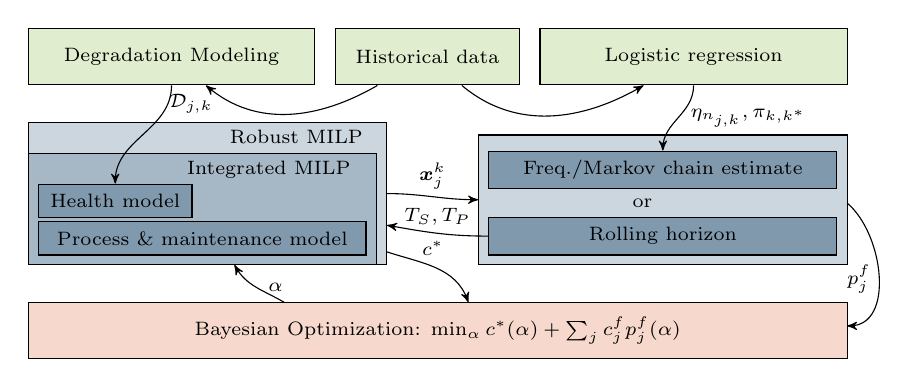
\begin{tikzpicture}[x=13mm, y=12mm ,>=stealth',bend angle=45,auto]
		\definecolor{mred}{RGB}{210,63,0}
		\definecolor{mblue}{RGB}{0,52,92}
		\definecolor{mgreen}{RGB}{102,164,10}
		\scriptsize


		% Bayesian optimization
		\node[draw, fit={(0,0) (8,0.6)},
			inner sep=0pt,
			label=center:{Bayesian Optimization: $\min_{\alpha} c^*(\alpha) + \sum_j c^f_j p^f_j(\alpha)$},
			fill=mred!20,
			align=center
			] (bo) {};

		% Robust MILP
		\node[draw, fit={(0,1) (3.5,2.5)},
			inner sep=0pt,
			fill=mblue!20
			] (rob) {};
			\node[anchor=center] at (2.62, 2.35) {Robust MILP};
		% Integrated MILP
		\node[draw, fit={(0,1) (3.4,2.17)},
			inner sep=0pt,
			fill=mblue!35
			] (int) {};
		\node[draw, fit={(0.1,1.1) (3.3,1.45)},
			inner sep=0pt,
			align=center,
			label=center:{Process \& maintenance model},
			fill=mblue!50
			] (pmm) {};
			%edge [-|] node [left] {$c^*(\alpha)$} (bo);
			\node[anchor=center] at (2.35, 2.0) {Integrated MILP};
		\node[draw, fit={(0.1,1.50) (1.60,1.85)},
			inner sep=0pt,
			label=center:{Health model},
			fill=mblue!50
			] (hm) {};

		% Estimating p^f
		\node[draw, fit={(4.4,1.0) (8.0,2.37)},
			inner sep=0pt,
			fill=mblue!20
			] (pf) {};
			%edge [<-] node [above] {$\boldsymbol{x}^k_j$} (rob);
		\node[draw, fit={(4.5,1.1) (7.9,1.5)},
			inner sep=0pt,
			fill=mblue!50,
			label=center:{Rolling horizon}
			] (rr) {};
		\node[draw, fit={(4.5,1.8) (7.9,2.2)},
			inner sep=0pt,
			fill=mblue!50,
			label=center:{Freq./Markov chain estimate}
			] (mc) {};
		\node[anchor=center] at (6.0, 1.65) {or};

		% Inputs
		\node[draw, fit={(0.0,2.9) (2.8,3.5)},
			inner sep=0pt,
			fill=mgreen!20,
			label=center:{Degradation Modeling}
			] (dm) {} edge[out=270,in=90,->] node [yshift=2.2em,xshift=0.8em,below right] {$\mathcal{D}_{j,k}$} (hm);
		\node[draw, fit={(5.0,2.9) (8.0,3.5)},
			inner sep=0pt,
			fill=mgreen!20,
			label=center:{Logistic regression}
			] (lr) {};
		\node[draw, fit={(3.0,2.9) (4.8,3.5)},
			inner sep=0pt,
			fill=mgreen!20,
			label=center:{Historical data}
			] (pd) {}
			edge[out=210,in=320,->] (dm)
			edge[out=320,in=210,->] (lr);

		% Edges
		\coordinate (bo-a) at (4.3, 0.6) {};
		\draw (8,1.65) edge[out=320,in=0,->] node [left,yshift=-0.15em] {$p^f_j$} (8.0, 0.35);
		\draw (rob) edge[out=342,in=110,->] node [yshift=0.9em,xshift=-1.0em,right] {$c^*$} (bo-a);
		\draw (2.5,0.6) edge[out=150,in=300,->] node [xshift=0.2em,right] {$\alpha$} (int);
		\draw (rob) edge[out=0,in=180,->] node [above] {$\boldsymbol{x}^k_j$} (pf);
		\draw (rr) edge[out=180,in=350,->] node [above] {$T_S,T_P$} (rob);
		\draw (lr) edge[out=270,in=90,->] node [xshift=0.2em,right] {$\eta_{n_{j,k}},\pi_{k,k^*}$} (mc);
	\end{tikzpicture}
%\end{document}

        \centering
        \visible<2>{
        {\huge Thank You!\\}
            {\tiny Funding: EP/L016796/1, EP/R511961/1 no.~17000145, and
            EP/P016871/1}
    \tikzexternaldisable
    \begin{tikzpicture}[overlay, remember picture]
    \node[anchor=north west, %anchor is upper left corner of the graphic
        xshift=7pt, %shifting around
        yshift=-216pt]
       at (current page.north west) %left upper corner of the page
       {
\includegraphics[width=0.29\textwidth]{Imperial_1_Pantone_solid.eps}};
    \end{tikzpicture}
    \begin{tikzpicture}[overlay, remember picture]
    \node[anchor=north east, %anchor is upper left corner of the graphic
        xshift=-170pt, %shifting around
        yshift=-214pt]
       at (current page.north east) %left upper corner of the page
       {
\includegraphics[width=0.23\textwidth]{COG_logo}};
    \end{tikzpicture}
    \begin{tikzpicture}[overlay, remember picture]
    \node[anchor=north east, %anchor is upper left corner of the graphic
        xshift=-88pt, %shifting around
        yshift=-220pt]
       at (current page.north east) %left upper corner of the page
       {
\includegraphics[width=0.23\textwidth]{logo_hipeds_v3.pdf}};
    \end{tikzpicture}
    \begin{tikzpicture}[overlay, remember picture]
    \node[anchor=north east, %anchor is upper left corner of the graphic
    xshift=-4pt, %shifting around
    yshift=-220pt]
    at (current page.north east) %left upper corner of the page
    {
\includegraphics[width=0.23\textwidth]{Schlumberger}};
    \end{tikzpicture}
    \tikzexternalenable
}
\end{frame}

\appendix
\begin{frame}[allowframebreaks]
    \tiny
    \bibliographystyle{apalike}
    \bibliography{lit_manual,lit}
\end{frame}

\begin{frame}{Degradation modelling}
    \centering
    \tikzsetnextfilename{deg-sig2}
    % Created by tikzDevice version 0.11 on 2018-05-22 16:51:31
% !TEX encoding = UTF-8 Unicode
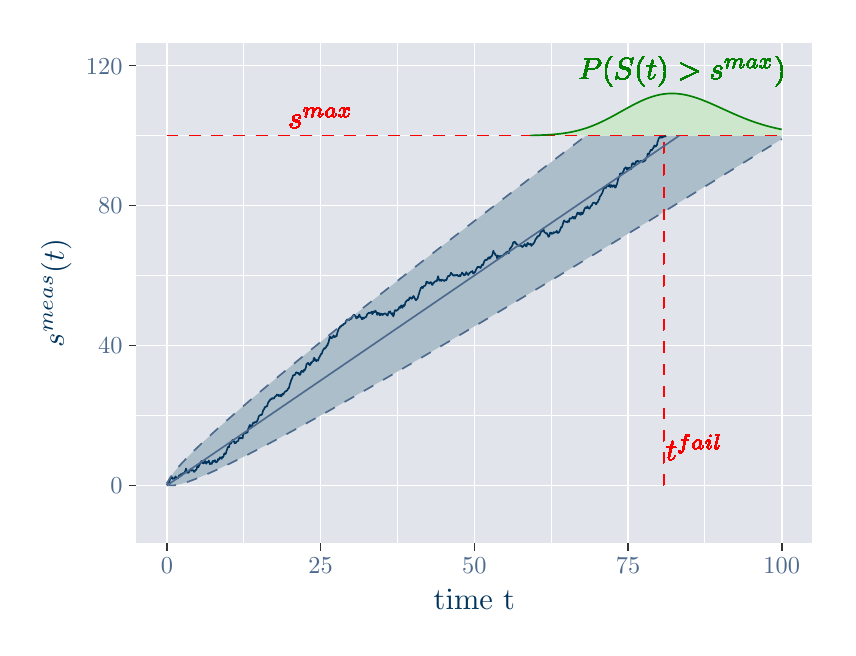
\begin{tikzpicture}[x=1pt,y=1pt]
\definecolor{fillColor}{RGB}{255,255,255}
\path[use as bounding box,fill=fillColor,fill opacity=0.00] (0,0) rectangle (289.08,216.81);
\begin{scope}
\path[clip] (  0.00,  0.00) rectangle (289.08,216.81);
\definecolor{drawColor}{RGB}{255,255,255}
\definecolor{fillColor}{RGB}{255,255,255}

\path[draw=drawColor,line width= 0.6pt,line join=round,line cap=round,fill=fillColor] (  0.00,  0.00) rectangle (289.08,216.81);
\end{scope}
\begin{scope}
\path[clip] ( 39.22, 30.56) rectangle (283.58,211.31);
\definecolor{fillColor}{RGB}{225,229,235}

\path[fill=fillColor] ( 39.22, 30.56) rectangle (283.58,211.31);
\definecolor{drawColor}{RGB}{255,255,255}

\path[draw=drawColor,line width= 0.3pt,line join=round] ( 39.22, 76.69) --
	(283.58, 76.69);

\path[draw=drawColor,line width= 0.3pt,line join=round] ( 39.22,127.25) --
	(283.58,127.25);

\path[draw=drawColor,line width= 0.3pt,line join=round] ( 39.22,177.81) --
	(283.58,177.81);

\path[draw=drawColor,line width= 0.3pt,line join=round] ( 78.10, 30.56) --
	( 78.10,211.31);

\path[draw=drawColor,line width= 0.3pt,line join=round] (133.63, 30.56) --
	(133.63,211.31);

\path[draw=drawColor,line width= 0.3pt,line join=round] (189.17, 30.56) --
	(189.17,211.31);

\path[draw=drawColor,line width= 0.3pt,line join=round] (244.70, 30.56) --
	(244.70,211.31);

\path[draw=drawColor,line width= 0.6pt,line join=round] ( 39.22, 51.41) --
	(283.58, 51.41);

\path[draw=drawColor,line width= 0.6pt,line join=round] ( 39.22,101.97) --
	(283.58,101.97);

\path[draw=drawColor,line width= 0.6pt,line join=round] ( 39.22,152.53) --
	(283.58,152.53);

\path[draw=drawColor,line width= 0.6pt,line join=round] ( 39.22,203.09) --
	(283.58,203.09);

\path[draw=drawColor,line width= 0.6pt,line join=round] ( 50.33, 30.56) --
	( 50.33,211.31);

\path[draw=drawColor,line width= 0.6pt,line join=round] (105.87, 30.56) --
	(105.87,211.31);

\path[draw=drawColor,line width= 0.6pt,line join=round] (161.40, 30.56) --
	(161.40,211.31);

\path[draw=drawColor,line width= 0.6pt,line join=round] (216.94, 30.56) --
	(216.94,211.31);

\path[draw=drawColor,line width= 0.6pt,line join=round] (272.47, 30.56) --
	(272.47,211.31);
\definecolor{fillColor}{RGB}{173,190,203}

\path[fill=fillColor] ( 50.33, 51.41) --
	( 50.55, 52.45) --
	( 50.77, 52.96) --
	( 51.00, 53.39) --
	( 51.22, 53.78) --
	( 51.44, 54.14) --
	( 51.66, 54.48) --
	( 51.88, 54.80) --
	( 52.11, 55.12) --
	( 52.33, 55.42) --
	( 52.55, 55.71) --
	( 52.77, 56.00) --
	( 53.00, 56.28) --
	( 53.22, 56.56) --
	( 53.44, 56.83) --
	( 53.66, 57.10) --
	( 53.88, 57.36) --
	( 54.11, 57.62) --
	( 54.33, 57.88) --
	( 54.55, 58.13) --
	( 54.77, 58.38) --
	( 54.99, 58.63) --
	( 55.22, 58.88) --
	( 55.44, 59.12) --
	( 55.66, 59.36) --
	( 55.88, 59.60) --
	( 56.11, 59.84) --
	( 56.33, 60.08) --
	( 56.55, 60.31) --
	( 56.77, 60.55) --
	( 56.99, 60.78) --
	( 57.22, 61.01) --
	( 57.44, 61.24) --
	( 57.66, 61.47) --
	( 57.88, 61.70) --
	( 58.10, 61.93) --
	( 58.33, 62.15) --
	( 58.55, 62.38) --
	( 58.77, 62.60) --
	( 58.99, 62.82) --
	( 59.22, 63.04) --
	( 59.44, 63.26) --
	( 59.66, 63.48) --
	( 59.88, 63.70) --
	( 60.10, 63.92) --
	( 60.33, 64.14) --
	( 60.55, 64.36) --
	( 60.77, 64.57) --
	( 60.99, 64.79) --
	( 61.21, 65.00) --
	( 61.44, 65.22) --
	( 61.66, 65.43) --
	( 61.88, 65.64) --
	( 62.10, 65.86) --
	( 62.33, 66.07) --
	( 62.55, 66.28) --
	( 62.77, 66.49) --
	( 62.99, 66.70) --
	( 63.21, 66.91) --
	( 63.44, 67.12) --
	( 63.66, 67.33) --
	( 63.88, 67.54) --
	( 64.10, 67.74) --
	( 64.32, 67.95) --
	( 64.55, 68.16) --
	( 64.77, 68.36) --
	( 64.99, 68.57) --
	( 65.21, 68.78) --
	( 65.44, 68.98) --
	( 65.66, 69.19) --
	( 65.88, 69.39) --
	( 66.10, 69.59) --
	( 66.32, 69.80) --
	( 66.55, 70.00) --
	( 66.77, 70.20) --
	( 66.99, 70.41) --
	( 67.21, 70.61) --
	( 67.43, 70.81) --
	( 67.66, 71.01) --
	( 67.88, 71.21) --
	( 68.10, 71.41) --
	( 68.32, 71.61) --
	( 68.55, 71.82) --
	( 68.77, 72.02) --
	( 68.99, 72.22) --
	( 69.21, 72.41) --
	( 69.43, 72.61) --
	( 69.66, 72.81) --
	( 69.88, 73.01) --
	( 70.10, 73.21) --
	( 70.32, 73.41) --
	( 70.54, 73.61) --
	( 70.77, 73.80) --
	( 70.99, 74.00) --
	( 71.21, 74.20) --
	( 71.43, 74.40) --
	( 71.66, 74.59) --
	( 71.88, 74.79) --
	( 72.10, 74.98) --
	( 72.32, 75.18) --
	( 72.54, 75.38) --
	( 72.77, 75.57) --
	( 72.99, 75.77) --
	( 73.21, 75.96) --
	( 73.43, 76.16) --
	( 73.65, 76.35) --
	( 73.88, 76.55) --
	( 74.10, 76.74) --
	( 74.32, 76.93) --
	( 74.54, 77.13) --
	( 74.77, 77.32) --
	( 74.99, 77.52) --
	( 75.21, 77.71) --
	( 75.43, 77.90) --
	( 75.65, 78.10) --
	( 75.88, 78.29) --
	( 76.10, 78.48) --
	( 76.32, 78.67) --
	( 76.54, 78.87) --
	( 76.76, 79.06) --
	( 76.99, 79.25) --
	( 77.21, 79.44) --
	( 77.43, 79.63) --
	( 77.65, 79.82) --
	( 77.88, 80.02) --
	( 78.10, 80.21) --
	( 78.32, 80.40) --
	( 78.54, 80.59) --
	( 78.76, 80.78) --
	( 78.99, 80.97) --
	( 79.21, 81.16) --
	( 79.43, 81.35) --
	( 79.65, 81.54) --
	( 79.87, 81.73) --
	( 80.10, 81.92) --
	( 80.32, 82.11) --
	( 80.54, 82.30) --
	( 80.76, 82.49) --
	( 80.99, 82.68) --
	( 81.21, 82.87) --
	( 81.43, 83.05) --
	( 81.65, 83.24) --
	( 81.87, 83.43) --
	( 82.10, 83.62) --
	( 82.32, 83.81) --
	( 82.54, 84.00) --
	( 82.76, 84.19) --
	( 82.98, 84.37) --
	( 83.21, 84.56) --
	( 83.43, 84.75) --
	( 83.65, 84.94) --
	( 83.87, 85.12) --
	( 84.10, 85.31) --
	( 84.32, 85.50) --
	( 84.54, 85.69) --
	( 84.76, 85.87) --
	( 84.98, 86.06) --
	( 85.21, 86.25) --
	( 85.43, 86.43) --
	( 85.65, 86.62) --
	( 85.87, 86.81) --
	( 86.09, 86.99) --
	( 86.32, 87.18) --
	( 86.54, 87.37) --
	( 86.76, 87.55) --
	( 86.98, 87.74) --
	( 87.21, 87.92) --
	( 87.43, 88.11) --
	( 87.65, 88.29) --
	( 87.87, 88.48) --
	( 88.09, 88.67) --
	( 88.32, 88.85) --
	( 88.54, 89.04) --
	( 88.76, 89.22) --
	( 88.98, 89.41) --
	( 89.20, 89.59) --
	( 89.43, 89.78) --
	( 89.65, 89.96) --
	( 89.87, 90.15) --
	( 90.09, 90.33) --
	( 90.32, 90.51) --
	( 90.54, 90.70) --
	( 90.76, 90.88) --
	( 90.98, 91.07) --
	( 91.20, 91.25) --
	( 91.43, 91.44) --
	( 91.65, 91.62) --
	( 91.87, 91.80) --
	( 92.09, 91.99) --
	( 92.31, 92.17) --
	( 92.54, 92.35) --
	( 92.76, 92.54) --
	( 92.98, 92.72) --
	( 93.20, 92.91) --
	( 93.43, 93.09) --
	( 93.65, 93.27) --
	( 93.87, 93.45) --
	( 94.09, 93.64) --
	( 94.31, 93.82) --
	( 94.54, 94.00) --
	( 94.76, 94.19) --
	( 94.98, 94.37) --
	( 95.20, 94.55) --
	( 95.42, 94.73) --
	( 95.65, 94.92) --
	( 95.87, 95.10) --
	( 96.09, 95.28) --
	( 96.31, 95.46) --
	( 96.54, 95.65) --
	( 96.76, 95.83) --
	( 96.98, 96.01) --
	( 97.20, 96.19) --
	( 97.42, 96.37) --
	( 97.65, 96.56) --
	( 97.87, 96.74) --
	( 98.09, 96.92) --
	( 98.31, 97.10) --
	( 98.53, 97.28) --
	( 98.76, 97.46) --
	( 98.98, 97.65) --
	( 99.20, 97.83) --
	( 99.42, 98.01) --
	( 99.65, 98.19) --
	( 99.87, 98.37) --
	(100.09, 98.55) --
	(100.31, 98.73) --
	(100.53, 98.91) --
	(100.76, 99.09) --
	(100.98, 99.28) --
	(101.20, 99.46) --
	(101.42, 99.64) --
	(101.64, 99.82) --
	(101.87,100.00) --
	(102.09,100.18) --
	(102.31,100.36) --
	(102.53,100.54) --
	(102.76,100.72) --
	(102.98,100.90) --
	(103.20,101.08) --
	(103.42,101.26) --
	(103.64,101.44) --
	(103.87,101.62) --
	(104.09,101.80) --
	(104.31,101.98) --
	(104.53,102.16) --
	(104.75,102.34) --
	(104.98,102.52) --
	(105.20,102.70) --
	(105.42,102.88) --
	(105.64,103.06) --
	(105.87,103.24) --
	(106.09,103.42) --
	(106.31,103.60) --
	(106.53,103.78) --
	(106.75,103.96) --
	(106.98,104.14) --
	(107.20,104.31) --
	(107.42,104.49) --
	(107.64,104.67) --
	(107.86,104.85) --
	(108.09,105.03) --
	(108.31,105.21) --
	(108.53,105.39) --
	(108.75,105.57) --
	(108.98,105.75) --
	(109.20,105.92) --
	(109.42,106.10) --
	(109.64,106.28) --
	(109.86,106.46) --
	(110.09,106.64) --
	(110.31,106.82) --
	(110.53,107.00) --
	(110.75,107.17) --
	(110.97,107.35) --
	(111.20,107.53) --
	(111.42,107.71) --
	(111.64,107.89) --
	(111.86,108.07) --
	(112.09,108.24) --
	(112.31,108.42) --
	(112.53,108.60) --
	(112.75,108.78) --
	(112.97,108.96) --
	(113.20,109.13) --
	(113.42,109.31) --
	(113.64,109.49) --
	(113.86,109.67) --
	(114.08,109.84) --
	(114.31,110.02) --
	(114.53,110.20) --
	(114.75,110.38) --
	(114.97,110.55) --
	(115.20,110.73) --
	(115.42,110.91) --
	(115.64,111.09) --
	(115.86,111.26) --
	(116.08,111.44) --
	(116.31,111.62) --
	(116.53,111.80) --
	(116.75,111.97) --
	(116.97,112.15) --
	(117.19,112.33) --
	(117.42,112.50) --
	(117.64,112.68) --
	(117.86,112.86) --
	(118.08,113.03) --
	(118.31,113.21) --
	(118.53,113.39) --
	(118.75,113.56) --
	(118.97,113.74) --
	(119.19,113.92) --
	(119.42,114.09) --
	(119.64,114.27) --
	(119.86,114.45) --
	(120.08,114.62) --
	(120.30,114.80) --
	(120.53,114.98) --
	(120.75,115.15) --
	(120.97,115.33) --
	(121.19,115.51) --
	(121.42,115.68) --
	(121.64,115.86) --
	(121.86,116.04) --
	(122.08,116.21) --
	(122.30,116.39) --
	(122.53,116.56) --
	(122.75,116.74) --
	(122.97,116.92) --
	(123.19,117.09) --
	(123.41,117.27) --
	(123.64,117.44) --
	(123.86,117.62) --
	(124.08,117.79) --
	(124.30,117.97) --
	(124.53,118.15) --
	(124.75,118.32) --
	(124.97,118.50) --
	(125.19,118.67) --
	(125.41,118.85) --
	(125.64,119.02) --
	(125.86,119.20) --
	(126.08,119.38) --
	(126.30,119.55) --
	(126.52,119.73) --
	(126.75,119.90) --
	(126.97,120.08) --
	(127.19,120.25) --
	(127.41,120.43) --
	(127.64,120.60) --
	(127.86,120.78) --
	(128.08,120.95) --
	(128.30,121.13) --
	(128.52,121.30) --
	(128.75,121.48) --
	(128.97,121.65) --
	(129.19,121.83) --
	(129.41,122.00) --
	(129.63,122.18) --
	(129.86,122.35) --
	(130.08,122.53) --
	(130.30,122.70) --
	(130.52,122.88) --
	(130.75,123.05) --
	(130.97,123.23) --
	(131.19,123.40) --
	(131.41,123.58) --
	(131.63,123.75) --
	(131.86,123.93) --
	(132.08,124.10) --
	(132.30,124.28) --
	(132.52,124.45) --
	(132.74,124.63) --
	(132.97,124.80) --
	(133.19,124.97) --
	(133.41,125.15) --
	(133.63,125.32) --
	(133.86,125.50) --
	(134.08,125.67) --
	(134.30,125.85) --
	(134.52,126.02) --
	(134.74,126.19) --
	(134.97,126.37) --
	(135.19,126.54) --
	(135.41,126.72) --
	(135.63,126.89) --
	(135.85,127.07) --
	(136.08,127.24) --
	(136.30,127.41) --
	(136.52,127.59) --
	(136.74,127.76) --
	(136.97,127.94) --
	(137.19,128.11) --
	(137.41,128.28) --
	(137.63,128.46) --
	(137.85,128.63) --
	(138.08,128.80) --
	(138.30,128.98) --
	(138.52,129.15) --
	(138.74,129.33) --
	(138.96,129.50) --
	(139.19,129.67) --
	(139.41,129.85) --
	(139.63,130.02) --
	(139.85,130.19) --
	(140.08,130.37) --
	(140.30,130.54) --
	(140.52,130.72) --
	(140.74,130.89) --
	(140.96,131.06) --
	(141.19,131.24) --
	(141.41,131.41) --
	(141.63,131.58) --
	(141.85,131.76) --
	(142.07,131.93) --
	(142.30,132.10) --
	(142.52,132.28) --
	(142.74,132.45) --
	(142.96,132.62) --
	(143.19,132.80) --
	(143.41,132.97) --
	(143.63,133.14) --
	(143.85,133.31) --
	(144.07,133.49) --
	(144.30,133.66) --
	(144.52,133.83) --
	(144.74,134.01) --
	(144.96,134.18) --
	(145.18,134.35) --
	(145.41,134.53) --
	(145.63,134.70) --
	(145.85,134.87) --
	(146.07,135.04) --
	(146.30,135.22) --
	(146.52,135.39) --
	(146.74,135.56) --
	(146.96,135.74) --
	(147.18,135.91) --
	(147.41,136.08) --
	(147.63,136.25) --
	(147.85,136.43) --
	(148.07,136.60) --
	(148.29,136.77) --
	(148.52,136.94) --
	(148.74,137.12) --
	(148.96,137.29) --
	(149.18,137.46) --
	(149.41,137.63) --
	(149.63,137.81) --
	(149.85,137.98) --
	(150.07,138.15) --
	(150.29,138.32) --
	(150.52,138.50) --
	(150.74,138.67) --
	(150.96,138.84) --
	(151.18,139.01) --
	(151.40,139.19) --
	(151.63,139.36) --
	(151.85,139.53) --
	(152.07,139.70) --
	(152.29,139.88) --
	(152.52,140.05) --
	(152.74,140.22) --
	(152.96,140.39) --
	(153.18,140.56) --
	(153.40,140.74) --
	(153.63,140.91) --
	(153.85,141.08) --
	(154.07,141.25) --
	(154.29,141.42) --
	(154.51,141.60) --
	(154.74,141.77) --
	(154.96,141.94) --
	(155.18,142.11) --
	(155.40,142.28) --
	(155.63,142.46) --
	(155.85,142.63) --
	(156.07,142.80) --
	(156.29,142.97) --
	(156.51,143.14) --
	(156.74,143.31) --
	(156.96,143.49) --
	(157.18,143.66) --
	(157.40,143.83) --
	(157.62,144.00) --
	(157.85,144.17) --
	(158.07,144.35) --
	(158.29,144.52) --
	(158.51,144.69) --
	(158.74,144.86) --
	(158.96,145.03) --
	(159.18,145.20) --
	(159.40,145.37) --
	(159.62,145.55) --
	(159.85,145.72) --
	(160.07,145.89) --
	(160.29,146.06) --
	(160.51,146.23) --
	(160.73,146.40) --
	(160.96,146.57) --
	(161.18,146.75) --
	(161.40,146.92) --
	(161.62,147.09) --
	(161.85,147.26) --
	(162.07,147.43) --
	(162.29,147.60) --
	(162.51,147.77) --
	(162.73,147.95) --
	(162.96,148.12) --
	(163.18,148.29) --
	(163.40,148.46) --
	(163.62,148.63) --
	(163.84,148.80) --
	(164.07,148.97) --
	(164.29,149.14) --
	(164.51,149.31) --
	(164.73,149.49) --
	(164.96,149.66) --
	(165.18,149.83) --
	(165.40,150.00) --
	(165.62,150.17) --
	(165.84,150.34) --
	(166.07,150.51) --
	(166.29,150.68) --
	(166.51,150.85) --
	(166.73,151.02) --
	(166.95,151.20) --
	(167.18,151.37) --
	(167.40,151.54) --
	(167.62,151.71) --
	(167.84,151.88) --
	(168.07,152.05) --
	(168.29,152.22) --
	(168.51,152.39) --
	(168.73,152.56) --
	(168.95,152.73) --
	(169.18,152.90) --
	(169.40,153.07) --
	(169.62,153.24) --
	(169.84,153.41) --
	(170.06,153.59) --
	(170.29,153.76) --
	(170.51,153.93) --
	(170.73,154.10) --
	(170.95,154.27) --
	(171.18,154.44) --
	(171.40,154.61) --
	(171.62,154.78) --
	(171.84,154.95) --
	(172.06,155.12) --
	(172.29,155.29) --
	(172.51,155.46) --
	(172.73,155.63) --
	(172.95,155.80) --
	(173.17,155.97) --
	(173.40,156.14) --
	(173.62,156.31) --
	(173.84,156.48) --
	(174.06,156.65) --
	(174.29,156.82) --
	(174.51,156.99) --
	(174.73,157.16) --
	(174.95,157.33) --
	(175.17,157.51) --
	(175.40,157.68) --
	(175.62,157.85) --
	(175.84,158.02) --
	(176.06,158.19) --
	(176.28,158.36) --
	(176.51,158.53) --
	(176.73,158.70) --
	(176.95,158.87) --
	(177.17,159.04) --
	(177.40,159.21) --
	(177.62,159.38) --
	(177.84,159.55) --
	(178.06,159.72) --
	(178.28,159.89) --
	(178.51,160.06) --
	(178.73,160.23) --
	(178.95,160.40) --
	(179.17,160.57) --
	(179.39,160.74) --
	(179.62,160.91) --
	(179.84,161.08) --
	(180.06,161.25) --
	(180.28,161.42) --
	(180.51,161.59) --
	(180.73,161.76) --
	(180.95,161.93) --
	(181.17,162.10) --
	(181.39,162.27) --
	(181.62,162.43) --
	(181.84,162.60) --
	(182.06,162.77) --
	(182.28,162.94) --
	(182.50,163.11) --
	(182.73,163.28) --
	(182.95,163.45) --
	(183.17,163.62) --
	(183.39,163.79) --
	(183.62,163.96) --
	(183.84,164.13) --
	(184.06,164.30) --
	(184.28,164.47) --
	(184.50,164.64) --
	(184.73,164.81) --
	(184.95,164.98) --
	(185.17,165.15) --
	(185.39,165.32) --
	(185.61,165.49) --
	(185.84,165.66) --
	(186.06,165.83) --
	(186.28,166.00) --
	(186.50,166.17) --
	(186.73,166.34) --
	(186.95,166.50) --
	(187.17,166.67) --
	(187.39,166.84) --
	(187.61,167.01) --
	(187.84,167.18) --
	(188.06,167.35) --
	(188.28,167.52) --
	(188.50,167.69) --
	(188.72,167.86) --
	(188.95,168.03) --
	(189.17,168.20) --
	(189.39,168.37) --
	(189.61,168.54) --
	(189.84,168.71) --
	(190.06,168.88) --
	(190.28,169.04) --
	(190.50,169.21) --
	(190.72,169.38) --
	(190.95,169.55) --
	(191.17,169.72) --
	(191.39,169.89) --
	(191.61,170.06) --
	(191.83,170.23) --
	(192.06,170.40) --
	(192.28,170.57) --
	(192.50,170.74) --
	(192.72,170.90) --
	(192.95,171.07) --
	(193.17,171.24) --
	(193.39,171.41) --
	(193.61,171.58) --
	(193.83,171.75) --
	(194.06,171.92) --
	(194.28,172.09) --
	(194.50,172.26) --
	(194.72,172.43) --
	(194.94,172.59) --
	(195.17,172.76) --
	(195.39,172.93) --
	(195.61,173.10) --
	(195.83,173.27) --
	(196.06,173.44) --
	(196.28,173.61) --
	(196.50,173.78) --
	(196.72,173.95) --
	(196.94,174.11) --
	(197.17,174.28) --
	(197.39,174.45) --
	(197.61,174.62) --
	(197.83,174.79) --
	(198.05,174.96) --
	(198.28,175.13) --
	(198.50,175.30) --
	(198.72,175.46) --
	(198.94,175.63) --
	(199.17,175.80) --
	(199.39,175.97) --
	(199.61,176.14) --
	(199.83,176.31) --
	(200.05,176.48) --
	(200.28,176.64) --
	(200.50,176.81) --
	(200.72,176.98) --
	(200.94,177.15) --
	(201.16,177.32) --
	(201.39,177.49) --
	(201.61,177.66) --
	(201.83,177.81) --
	(202.05,177.81) --
	(202.28,177.81) --
	(202.50,177.81) --
	(202.72,177.81) --
	(202.94,177.81) --
	(203.16,177.81) --
	(203.39,177.81) --
	(203.61,177.81) --
	(203.83,177.81) --
	(204.05,177.81) --
	(204.27,177.81) --
	(204.50,177.81) --
	(204.72,177.81) --
	(204.94,177.81) --
	(205.16,177.81) --
	(205.39,177.81) --
	(205.61,177.81) --
	(205.83,177.81) --
	(206.05,177.81) --
	(206.27,177.81) --
	(206.50,177.81) --
	(206.72,177.81) --
	(206.94,177.81) --
	(207.16,177.81) --
	(207.38,177.81) --
	(207.61,177.81) --
	(207.83,177.81) --
	(208.05,177.81) --
	(208.27,177.81) --
	(208.50,177.81) --
	(208.72,177.81) --
	(208.94,177.81) --
	(209.16,177.81) --
	(209.38,177.81) --
	(209.61,177.81) --
	(209.83,177.81) --
	(210.05,177.81) --
	(210.27,177.81) --
	(210.49,177.81) --
	(210.72,177.81) --
	(210.94,177.81) --
	(211.16,177.81) --
	(211.38,177.81) --
	(211.61,177.81) --
	(211.83,177.81) --
	(212.05,177.81) --
	(212.27,177.81) --
	(212.49,177.81) --
	(212.72,177.81) --
	(212.94,177.81) --
	(213.16,177.81) --
	(213.38,177.81) --
	(213.60,177.81) --
	(213.83,177.81) --
	(214.05,177.81) --
	(214.27,177.81) --
	(214.49,177.81) --
	(214.72,177.81) --
	(214.94,177.81) --
	(215.16,177.81) --
	(215.38,177.81) --
	(215.60,177.81) --
	(215.83,177.81) --
	(216.05,177.81) --
	(216.27,177.81) --
	(216.49,177.81) --
	(216.71,177.81) --
	(216.94,177.81) --
	(217.16,177.81) --
	(217.38,177.81) --
	(217.60,177.81) --
	(217.83,177.81) --
	(218.05,177.81) --
	(218.27,177.81) --
	(218.49,177.81) --
	(218.71,177.81) --
	(218.94,177.81) --
	(219.16,177.81) --
	(219.38,177.81) --
	(219.60,177.81) --
	(219.82,177.81) --
	(220.05,177.81) --
	(220.27,177.81) --
	(220.49,177.81) --
	(220.71,177.81) --
	(220.94,177.81) --
	(221.16,177.81) --
	(221.38,177.81) --
	(221.60,177.81) --
	(221.82,177.81) --
	(222.05,177.81) --
	(222.27,177.81) --
	(222.49,177.81) --
	(222.71,177.81) --
	(222.93,177.81) --
	(223.16,177.81) --
	(223.38,177.81) --
	(223.60,177.81) --
	(223.82,177.81) --
	(224.05,177.81) --
	(224.27,177.81) --
	(224.49,177.81) --
	(224.71,177.81) --
	(224.93,177.81) --
	(225.16,177.81) --
	(225.38,177.81) --
	(225.60,177.81) --
	(225.82,177.81) --
	(226.04,177.81) --
	(226.27,177.81) --
	(226.49,177.81) --
	(226.71,177.81) --
	(226.93,177.81) --
	(227.16,177.81) --
	(227.38,177.81) --
	(227.60,177.81) --
	(227.82,177.81) --
	(228.04,177.81) --
	(228.27,177.81) --
	(228.49,177.81) --
	(228.71,177.81) --
	(228.93,177.81) --
	(229.15,177.81) --
	(229.38,177.81) --
	(229.60,177.81) --
	(229.82,177.81) --
	(230.04,177.81) --
	(230.27,177.81) --
	(230.49,177.81) --
	(230.71,177.81) --
	(230.93,177.81) --
	(231.15,177.81) --
	(231.38,177.81) --
	(231.60,177.81) --
	(231.82,177.81) --
	(232.04,177.81) --
	(232.26,177.81) --
	(232.49,177.81) --
	(232.71,177.81) --
	(232.93,177.81) --
	(233.15,177.81) --
	(233.38,177.81) --
	(233.60,177.81) --
	(233.82,177.81) --
	(234.04,177.81) --
	(234.26,177.81) --
	(234.49,177.81) --
	(234.71,177.81) --
	(234.93,177.81) --
	(235.15,177.81) --
	(235.37,177.81) --
	(235.60,177.81) --
	(235.82,177.81) --
	(236.04,177.81) --
	(236.26,177.81) --
	(236.49,177.81) --
	(236.71,177.81) --
	(236.93,177.81) --
	(237.15,177.81) --
	(237.37,177.81) --
	(237.60,177.81) --
	(237.82,177.81) --
	(238.04,177.81) --
	(238.26,177.81) --
	(238.48,177.81) --
	(238.71,177.81) --
	(238.93,177.81) --
	(239.15,177.81) --
	(239.37,177.81) --
	(239.60,177.81) --
	(239.82,177.81) --
	(240.04,177.81) --
	(240.26,177.81) --
	(240.48,177.81) --
	(240.71,177.81) --
	(240.93,177.81) --
	(241.15,177.81) --
	(241.37,177.81) --
	(241.59,177.81) --
	(241.82,177.81) --
	(242.04,177.81) --
	(242.26,177.81) --
	(242.48,177.81) --
	(242.71,177.81) --
	(242.93,177.81) --
	(243.15,177.81) --
	(243.37,177.81) --
	(243.59,177.81) --
	(243.82,177.81) --
	(244.04,177.81) --
	(244.26,177.81) --
	(244.48,177.81) --
	(244.70,177.81) --
	(244.93,177.81) --
	(245.15,177.81) --
	(245.37,177.81) --
	(245.59,177.81) --
	(245.82,177.81) --
	(246.04,177.81) --
	(246.26,177.81) --
	(246.48,177.81) --
	(246.70,177.81) --
	(246.93,177.81) --
	(247.15,177.81) --
	(247.37,177.81) --
	(247.59,177.81) --
	(247.81,177.81) --
	(248.04,177.81) --
	(248.26,177.81) --
	(248.48,177.81) --
	(248.70,177.81) --
	(248.93,177.81) --
	(249.15,177.81) --
	(249.37,177.81) --
	(249.59,177.81) --
	(249.81,177.81) --
	(250.04,177.81) --
	(250.26,177.81) --
	(250.48,177.81) --
	(250.70,177.81) --
	(250.92,177.81) --
	(251.15,177.81) --
	(251.37,177.81) --
	(251.59,177.81) --
	(251.81,177.81) --
	(252.04,177.81) --
	(252.26,177.81) --
	(252.48,177.81) --
	(252.70,177.81) --
	(252.92,177.81) --
	(253.15,177.81) --
	(253.37,177.81) --
	(253.59,177.81) --
	(253.81,177.81) --
	(254.03,177.81) --
	(254.26,177.81) --
	(254.48,177.81) --
	(254.70,177.81) --
	(254.92,177.81) --
	(255.15,177.81) --
	(255.37,177.81) --
	(255.59,177.81) --
	(255.81,177.81) --
	(256.03,177.81) --
	(256.26,177.81) --
	(256.48,177.81) --
	(256.70,177.81) --
	(256.92,177.81) --
	(257.14,177.81) --
	(257.37,177.81) --
	(257.59,177.81) --
	(257.81,177.81) --
	(258.03,177.81) --
	(258.26,177.81) --
	(258.48,177.81) --
	(258.70,177.81) --
	(258.92,177.81) --
	(259.14,177.81) --
	(259.37,177.81) --
	(259.59,177.81) --
	(259.81,177.81) --
	(260.03,177.81) --
	(260.25,177.81) --
	(260.48,177.81) --
	(260.70,177.81) --
	(260.92,177.81) --
	(261.14,177.81) --
	(261.37,177.81) --
	(261.59,177.81) --
	(261.81,177.81) --
	(262.03,177.81) --
	(262.25,177.81) --
	(262.48,177.81) --
	(262.70,177.81) --
	(262.92,177.81) --
	(263.14,177.81) --
	(263.36,177.81) --
	(263.59,177.81) --
	(263.81,177.81) --
	(264.03,177.81) --
	(264.25,177.81) --
	(264.48,177.81) --
	(264.70,177.81) --
	(264.92,177.81) --
	(265.14,177.81) --
	(265.36,177.81) --
	(265.59,177.81) --
	(265.81,177.81) --
	(266.03,177.81) --
	(266.25,177.81) --
	(266.47,177.81) --
	(266.70,177.81) --
	(266.92,177.81) --
	(267.14,177.81) --
	(267.36,177.81) --
	(267.59,177.81) --
	(267.81,177.81) --
	(268.03,177.81) --
	(268.25,177.81) --
	(268.47,177.81) --
	(268.70,177.81) --
	(268.92,177.81) --
	(269.14,177.81) --
	(269.36,177.81) --
	(269.58,177.81) --
	(269.81,177.81) --
	(270.03,177.81) --
	(270.25,177.81) --
	(270.47,177.81) --
	(270.70,177.81) --
	(270.92,177.81) --
	(271.14,177.81) --
	(271.36,177.81) --
	(271.58,177.81) --
	(271.81,177.81) --
	(272.03,177.81) --
	(272.25,177.81) --
	(272.47,177.81) --
	(272.47,176.56) --
	(272.25,176.42) --
	(272.03,176.28) --
	(271.81,176.15) --
	(271.58,176.01) --
	(271.36,175.87) --
	(271.14,175.73) --
	(270.92,175.60) --
	(270.70,175.46) --
	(270.47,175.32) --
	(270.25,175.18) --
	(270.03,175.04) --
	(269.81,174.91) --
	(269.58,174.77) --
	(269.36,174.63) --
	(269.14,174.49) --
	(268.92,174.36) --
	(268.70,174.22) --
	(268.47,174.08) --
	(268.25,173.94) --
	(268.03,173.81) --
	(267.81,173.67) --
	(267.59,173.53) --
	(267.36,173.39) --
	(267.14,173.26) --
	(266.92,173.12) --
	(266.70,172.98) --
	(266.47,172.84) --
	(266.25,172.70) --
	(266.03,172.57) --
	(265.81,172.43) --
	(265.59,172.29) --
	(265.36,172.15) --
	(265.14,172.02) --
	(264.92,171.88) --
	(264.70,171.74) --
	(264.48,171.60) --
	(264.25,171.47) --
	(264.03,171.33) --
	(263.81,171.19) --
	(263.59,171.05) --
	(263.36,170.92) --
	(263.14,170.78) --
	(262.92,170.64) --
	(262.70,170.50) --
	(262.48,170.37) --
	(262.25,170.23) --
	(262.03,170.09) --
	(261.81,169.95) --
	(261.59,169.82) --
	(261.37,169.68) --
	(261.14,169.54) --
	(260.92,169.41) --
	(260.70,169.27) --
	(260.48,169.13) --
	(260.25,168.99) --
	(260.03,168.86) --
	(259.81,168.72) --
	(259.59,168.58) --
	(259.37,168.44) --
	(259.14,168.31) --
	(258.92,168.17) --
	(258.70,168.03) --
	(258.48,167.89) --
	(258.26,167.76) --
	(258.03,167.62) --
	(257.81,167.48) --
	(257.59,167.35) --
	(257.37,167.21) --
	(257.14,167.07) --
	(256.92,166.93) --
	(256.70,166.80) --
	(256.48,166.66) --
	(256.26,166.52) --
	(256.03,166.38) --
	(255.81,166.25) --
	(255.59,166.11) --
	(255.37,165.97) --
	(255.15,165.84) --
	(254.92,165.70) --
	(254.70,165.56) --
	(254.48,165.42) --
	(254.26,165.29) --
	(254.03,165.15) --
	(253.81,165.01) --
	(253.59,164.88) --
	(253.37,164.74) --
	(253.15,164.60) --
	(252.92,164.46) --
	(252.70,164.33) --
	(252.48,164.19) --
	(252.26,164.05) --
	(252.04,163.92) --
	(251.81,163.78) --
	(251.59,163.64) --
	(251.37,163.50) --
	(251.15,163.37) --
	(250.92,163.23) --
	(250.70,163.09) --
	(250.48,162.96) --
	(250.26,162.82) --
	(250.04,162.68) --
	(249.81,162.54) --
	(249.59,162.41) --
	(249.37,162.27) --
	(249.15,162.13) --
	(248.93,162.00) --
	(248.70,161.86) --
	(248.48,161.72) --
	(248.26,161.59) --
	(248.04,161.45) --
	(247.81,161.31) --
	(247.59,161.18) --
	(247.37,161.04) --
	(247.15,160.90) --
	(246.93,160.76) --
	(246.70,160.63) --
	(246.48,160.49) --
	(246.26,160.35) --
	(246.04,160.22) --
	(245.82,160.08) --
	(245.59,159.94) --
	(245.37,159.81) --
	(245.15,159.67) --
	(244.93,159.53) --
	(244.70,159.40) --
	(244.48,159.26) --
	(244.26,159.12) --
	(244.04,158.99) --
	(243.82,158.85) --
	(243.59,158.71) --
	(243.37,158.58) --
	(243.15,158.44) --
	(242.93,158.30) --
	(242.71,158.16) --
	(242.48,158.03) --
	(242.26,157.89) --
	(242.04,157.75) --
	(241.82,157.62) --
	(241.59,157.48) --
	(241.37,157.34) --
	(241.15,157.21) --
	(240.93,157.07) --
	(240.71,156.93) --
	(240.48,156.80) --
	(240.26,156.66) --
	(240.04,156.52) --
	(239.82,156.39) --
	(239.60,156.25) --
	(239.37,156.11) --
	(239.15,155.98) --
	(238.93,155.84) --
	(238.71,155.71) --
	(238.48,155.57) --
	(238.26,155.43) --
	(238.04,155.30) --
	(237.82,155.16) --
	(237.60,155.02) --
	(237.37,154.89) --
	(237.15,154.75) --
	(236.93,154.61) --
	(236.71,154.48) --
	(236.49,154.34) --
	(236.26,154.20) --
	(236.04,154.07) --
	(235.82,153.93) --
	(235.60,153.79) --
	(235.37,153.66) --
	(235.15,153.52) --
	(234.93,153.38) --
	(234.71,153.25) --
	(234.49,153.11) --
	(234.26,152.98) --
	(234.04,152.84) --
	(233.82,152.70) --
	(233.60,152.57) --
	(233.38,152.43) --
	(233.15,152.29) --
	(232.93,152.16) --
	(232.71,152.02) --
	(232.49,151.88) --
	(232.26,151.75) --
	(232.04,151.61) --
	(231.82,151.48) --
	(231.60,151.34) --
	(231.38,151.20) --
	(231.15,151.07) --
	(230.93,150.93) --
	(230.71,150.79) --
	(230.49,150.66) --
	(230.27,150.52) --
	(230.04,150.39) --
	(229.82,150.25) --
	(229.60,150.11) --
	(229.38,149.98) --
	(229.15,149.84) --
	(228.93,149.70) --
	(228.71,149.57) --
	(228.49,149.43) --
	(228.27,149.30) --
	(228.04,149.16) --
	(227.82,149.02) --
	(227.60,148.89) --
	(227.38,148.75) --
	(227.16,148.62) --
	(226.93,148.48) --
	(226.71,148.34) --
	(226.49,148.21) --
	(226.27,148.07) --
	(226.04,147.93) --
	(225.82,147.80) --
	(225.60,147.66) --
	(225.38,147.53) --
	(225.16,147.39) --
	(224.93,147.25) --
	(224.71,147.12) --
	(224.49,146.98) --
	(224.27,146.85) --
	(224.05,146.71) --
	(223.82,146.58) --
	(223.60,146.44) --
	(223.38,146.30) --
	(223.16,146.17) --
	(222.93,146.03) --
	(222.71,145.90) --
	(222.49,145.76) --
	(222.27,145.62) --
	(222.05,145.49) --
	(221.82,145.35) --
	(221.60,145.22) --
	(221.38,145.08) --
	(221.16,144.94) --
	(220.94,144.81) --
	(220.71,144.67) --
	(220.49,144.54) --
	(220.27,144.40) --
	(220.05,144.27) --
	(219.82,144.13) --
	(219.60,143.99) --
	(219.38,143.86) --
	(219.16,143.72) --
	(218.94,143.59) --
	(218.71,143.45) --
	(218.49,143.32) --
	(218.27,143.18) --
	(218.05,143.04) --
	(217.83,142.91) --
	(217.60,142.77) --
	(217.38,142.64) --
	(217.16,142.50) --
	(216.94,142.37) --
	(216.71,142.23) --
	(216.49,142.09) --
	(216.27,141.96) --
	(216.05,141.82) --
	(215.83,141.69) --
	(215.60,141.55) --
	(215.38,141.42) --
	(215.16,141.28) --
	(214.94,141.15) --
	(214.72,141.01) --
	(214.49,140.87) --
	(214.27,140.74) --
	(214.05,140.60) --
	(213.83,140.47) --
	(213.60,140.33) --
	(213.38,140.20) --
	(213.16,140.06) --
	(212.94,139.93) --
	(212.72,139.79) --
	(212.49,139.66) --
	(212.27,139.52) --
	(212.05,139.38) --
	(211.83,139.25) --
	(211.61,139.11) --
	(211.38,138.98) --
	(211.16,138.84) --
	(210.94,138.71) --
	(210.72,138.57) --
	(210.49,138.44) --
	(210.27,138.30) --
	(210.05,138.17) --
	(209.83,138.03) --
	(209.61,137.90) --
	(209.38,137.76) --
	(209.16,137.63) --
	(208.94,137.49) --
	(208.72,137.36) --
	(208.50,137.22) --
	(208.27,137.08) --
	(208.05,136.95) --
	(207.83,136.81) --
	(207.61,136.68) --
	(207.38,136.54) --
	(207.16,136.41) --
	(206.94,136.27) --
	(206.72,136.14) --
	(206.50,136.00) --
	(206.27,135.87) --
	(206.05,135.73) --
	(205.83,135.60) --
	(205.61,135.46) --
	(205.39,135.33) --
	(205.16,135.19) --
	(204.94,135.06) --
	(204.72,134.92) --
	(204.50,134.79) --
	(204.27,134.65) --
	(204.05,134.52) --
	(203.83,134.38) --
	(203.61,134.25) --
	(203.39,134.11) --
	(203.16,133.98) --
	(202.94,133.84) --
	(202.72,133.71) --
	(202.50,133.57) --
	(202.28,133.44) --
	(202.05,133.30) --
	(201.83,133.17) --
	(201.61,133.03) --
	(201.39,132.90) --
	(201.16,132.76) --
	(200.94,132.63) --
	(200.72,132.50) --
	(200.50,132.36) --
	(200.28,132.23) --
	(200.05,132.09) --
	(199.83,131.96) --
	(199.61,131.82) --
	(199.39,131.69) --
	(199.17,131.55) --
	(198.94,131.42) --
	(198.72,131.28) --
	(198.50,131.15) --
	(198.28,131.01) --
	(198.05,130.88) --
	(197.83,130.74) --
	(197.61,130.61) --
	(197.39,130.47) --
	(197.17,130.34) --
	(196.94,130.21) --
	(196.72,130.07) --
	(196.50,129.94) --
	(196.28,129.80) --
	(196.06,129.67) --
	(195.83,129.53) --
	(195.61,129.40) --
	(195.39,129.26) --
	(195.17,129.13) --
	(194.94,129.00) --
	(194.72,128.86) --
	(194.50,128.73) --
	(194.28,128.59) --
	(194.06,128.46) --
	(193.83,128.32) --
	(193.61,128.19) --
	(193.39,128.05) --
	(193.17,127.92) --
	(192.95,127.79) --
	(192.72,127.65) --
	(192.50,127.52) --
	(192.28,127.38) --
	(192.06,127.25) --
	(191.83,127.11) --
	(191.61,126.98) --
	(191.39,126.85) --
	(191.17,126.71) --
	(190.95,126.58) --
	(190.72,126.44) --
	(190.50,126.31) --
	(190.28,126.17) --
	(190.06,126.04) --
	(189.84,125.91) --
	(189.61,125.77) --
	(189.39,125.64) --
	(189.17,125.50) --
	(188.95,125.37) --
	(188.72,125.24) --
	(188.50,125.10) --
	(188.28,124.97) --
	(188.06,124.83) --
	(187.84,124.70) --
	(187.61,124.57) --
	(187.39,124.43) --
	(187.17,124.30) --
	(186.95,124.16) --
	(186.73,124.03) --
	(186.50,123.90) --
	(186.28,123.76) --
	(186.06,123.63) --
	(185.84,123.49) --
	(185.61,123.36) --
	(185.39,123.23) --
	(185.17,123.09) --
	(184.95,122.96) --
	(184.73,122.82) --
	(184.50,122.69) --
	(184.28,122.56) --
	(184.06,122.42) --
	(183.84,122.29) --
	(183.62,122.16) --
	(183.39,122.02) --
	(183.17,121.89) --
	(182.95,121.76) --
	(182.73,121.62) --
	(182.50,121.49) --
	(182.28,121.35) --
	(182.06,121.22) --
	(181.84,121.09) --
	(181.62,120.95) --
	(181.39,120.82) --
	(181.17,120.69) --
	(180.95,120.55) --
	(180.73,120.42) --
	(180.51,120.29) --
	(180.28,120.15) --
	(180.06,120.02) --
	(179.84,119.88) --
	(179.62,119.75) --
	(179.39,119.62) --
	(179.17,119.48) --
	(178.95,119.35) --
	(178.73,119.22) --
	(178.51,119.08) --
	(178.28,118.95) --
	(178.06,118.82) --
	(177.84,118.68) --
	(177.62,118.55) --
	(177.40,118.42) --
	(177.17,118.28) --
	(176.95,118.15) --
	(176.73,118.02) --
	(176.51,117.88) --
	(176.28,117.75) --
	(176.06,117.62) --
	(175.84,117.49) --
	(175.62,117.35) --
	(175.40,117.22) --
	(175.17,117.09) --
	(174.95,116.95) --
	(174.73,116.82) --
	(174.51,116.69) --
	(174.29,116.55) --
	(174.06,116.42) --
	(173.84,116.29) --
	(173.62,116.15) --
	(173.40,116.02) --
	(173.17,115.89) --
	(172.95,115.76) --
	(172.73,115.62) --
	(172.51,115.49) --
	(172.29,115.36) --
	(172.06,115.22) --
	(171.84,115.09) --
	(171.62,114.96) --
	(171.40,114.82) --
	(171.18,114.69) --
	(170.95,114.56) --
	(170.73,114.43) --
	(170.51,114.29) --
	(170.29,114.16) --
	(170.06,114.03) --
	(169.84,113.90) --
	(169.62,113.76) --
	(169.40,113.63) --
	(169.18,113.50) --
	(168.95,113.36) --
	(168.73,113.23) --
	(168.51,113.10) --
	(168.29,112.97) --
	(168.07,112.83) --
	(167.84,112.70) --
	(167.62,112.57) --
	(167.40,112.44) --
	(167.18,112.30) --
	(166.95,112.17) --
	(166.73,112.04) --
	(166.51,111.91) --
	(166.29,111.77) --
	(166.07,111.64) --
	(165.84,111.51) --
	(165.62,111.38) --
	(165.40,111.24) --
	(165.18,111.11) --
	(164.96,110.98) --
	(164.73,110.85) --
	(164.51,110.72) --
	(164.29,110.58) --
	(164.07,110.45) --
	(163.84,110.32) --
	(163.62,110.19) --
	(163.40,110.05) --
	(163.18,109.92) --
	(162.96,109.79) --
	(162.73,109.66) --
	(162.51,109.53) --
	(162.29,109.39) --
	(162.07,109.26) --
	(161.85,109.13) --
	(161.62,109.00) --
	(161.40,108.86) --
	(161.18,108.73) --
	(160.96,108.60) --
	(160.73,108.47) --
	(160.51,108.34) --
	(160.29,108.21) --
	(160.07,108.07) --
	(159.85,107.94) --
	(159.62,107.81) --
	(159.40,107.68) --
	(159.18,107.55) --
	(158.96,107.41) --
	(158.74,107.28) --
	(158.51,107.15) --
	(158.29,107.02) --
	(158.07,106.89) --
	(157.85,106.76) --
	(157.62,106.62) --
	(157.40,106.49) --
	(157.18,106.36) --
	(156.96,106.23) --
	(156.74,106.10) --
	(156.51,105.97) --
	(156.29,105.83) --
	(156.07,105.70) --
	(155.85,105.57) --
	(155.63,105.44) --
	(155.40,105.31) --
	(155.18,105.18) --
	(154.96,105.05) --
	(154.74,104.91) --
	(154.51,104.78) --
	(154.29,104.65) --
	(154.07,104.52) --
	(153.85,104.39) --
	(153.63,104.26) --
	(153.40,104.13) --
	(153.18,103.99) --
	(152.96,103.86) --
	(152.74,103.73) --
	(152.52,103.60) --
	(152.29,103.47) --
	(152.07,103.34) --
	(151.85,103.21) --
	(151.63,103.08) --
	(151.40,102.95) --
	(151.18,102.81) --
	(150.96,102.68) --
	(150.74,102.55) --
	(150.52,102.42) --
	(150.29,102.29) --
	(150.07,102.16) --
	(149.85,102.03) --
	(149.63,101.90) --
	(149.41,101.77) --
	(149.18,101.64) --
	(148.96,101.50) --
	(148.74,101.37) --
	(148.52,101.24) --
	(148.29,101.11) --
	(148.07,100.98) --
	(147.85,100.85) --
	(147.63,100.72) --
	(147.41,100.59) --
	(147.18,100.46) --
	(146.96,100.33) --
	(146.74,100.20) --
	(146.52,100.07) --
	(146.30, 99.94) --
	(146.07, 99.81) --
	(145.85, 99.68) --
	(145.63, 99.55) --
	(145.41, 99.41) --
	(145.18, 99.28) --
	(144.96, 99.15) --
	(144.74, 99.02) --
	(144.52, 98.89) --
	(144.30, 98.76) --
	(144.07, 98.63) --
	(143.85, 98.50) --
	(143.63, 98.37) --
	(143.41, 98.24) --
	(143.19, 98.11) --
	(142.96, 97.98) --
	(142.74, 97.85) --
	(142.52, 97.72) --
	(142.30, 97.59) --
	(142.07, 97.46) --
	(141.85, 97.33) --
	(141.63, 97.20) --
	(141.41, 97.07) --
	(141.19, 96.94) --
	(140.96, 96.81) --
	(140.74, 96.68) --
	(140.52, 96.55) --
	(140.30, 96.42) --
	(140.08, 96.29) --
	(139.85, 96.16) --
	(139.63, 96.03) --
	(139.41, 95.90) --
	(139.19, 95.77) --
	(138.96, 95.64) --
	(138.74, 95.51) --
	(138.52, 95.38) --
	(138.30, 95.25) --
	(138.08, 95.12) --
	(137.85, 95.00) --
	(137.63, 94.87) --
	(137.41, 94.74) --
	(137.19, 94.61) --
	(136.97, 94.48) --
	(136.74, 94.35) --
	(136.52, 94.22) --
	(136.30, 94.09) --
	(136.08, 93.96) --
	(135.85, 93.83) --
	(135.63, 93.70) --
	(135.41, 93.57) --
	(135.19, 93.44) --
	(134.97, 93.31) --
	(134.74, 93.18) --
	(134.52, 93.06) --
	(134.30, 92.93) --
	(134.08, 92.80) --
	(133.86, 92.67) --
	(133.63, 92.54) --
	(133.41, 92.41) --
	(133.19, 92.28) --
	(132.97, 92.15) --
	(132.74, 92.02) --
	(132.52, 91.89) --
	(132.30, 91.77) --
	(132.08, 91.64) --
	(131.86, 91.51) --
	(131.63, 91.38) --
	(131.41, 91.25) --
	(131.19, 91.12) --
	(130.97, 90.99) --
	(130.75, 90.87) --
	(130.52, 90.74) --
	(130.30, 90.61) --
	(130.08, 90.48) --
	(129.86, 90.35) --
	(129.63, 90.22) --
	(129.41, 90.09) --
	(129.19, 89.97) --
	(128.97, 89.84) --
	(128.75, 89.71) --
	(128.52, 89.58) --
	(128.30, 89.45) --
	(128.08, 89.32) --
	(127.86, 89.20) --
	(127.64, 89.07) --
	(127.41, 88.94) --
	(127.19, 88.81) --
	(126.97, 88.68) --
	(126.75, 88.56) --
	(126.52, 88.43) --
	(126.30, 88.30) --
	(126.08, 88.17) --
	(125.86, 88.04) --
	(125.64, 87.92) --
	(125.41, 87.79) --
	(125.19, 87.66) --
	(124.97, 87.53) --
	(124.75, 87.41) --
	(124.53, 87.28) --
	(124.30, 87.15) --
	(124.08, 87.02) --
	(123.86, 86.90) --
	(123.64, 86.77) --
	(123.41, 86.64) --
	(123.19, 86.51) --
	(122.97, 86.39) --
	(122.75, 86.26) --
	(122.53, 86.13) --
	(122.30, 86.00) --
	(122.08, 85.88) --
	(121.86, 85.75) --
	(121.64, 85.62) --
	(121.42, 85.50) --
	(121.19, 85.37) --
	(120.97, 85.24) --
	(120.75, 85.11) --
	(120.53, 84.99) --
	(120.30, 84.86) --
	(120.08, 84.73) --
	(119.86, 84.61) --
	(119.64, 84.48) --
	(119.42, 84.35) --
	(119.19, 84.23) --
	(118.97, 84.10) --
	(118.75, 83.97) --
	(118.53, 83.85) --
	(118.31, 83.72) --
	(118.08, 83.59) --
	(117.86, 83.47) --
	(117.64, 83.34) --
	(117.42, 83.21) --
	(117.19, 83.09) --
	(116.97, 82.96) --
	(116.75, 82.83) --
	(116.53, 82.71) --
	(116.31, 82.58) --
	(116.08, 82.46) --
	(115.86, 82.33) --
	(115.64, 82.20) --
	(115.42, 82.08) --
	(115.20, 81.95) --
	(114.97, 81.83) --
	(114.75, 81.70) --
	(114.53, 81.57) --
	(114.31, 81.45) --
	(114.08, 81.32) --
	(113.86, 81.20) --
	(113.64, 81.07) --
	(113.42, 80.95) --
	(113.20, 80.82) --
	(112.97, 80.69) --
	(112.75, 80.57) --
	(112.53, 80.44) --
	(112.31, 80.32) --
	(112.09, 80.19) --
	(111.86, 80.07) --
	(111.64, 79.94) --
	(111.42, 79.82) --
	(111.20, 79.69) --
	(110.97, 79.57) --
	(110.75, 79.44) --
	(110.53, 79.32) --
	(110.31, 79.19) --
	(110.09, 79.07) --
	(109.86, 78.94) --
	(109.64, 78.82) --
	(109.42, 78.69) --
	(109.20, 78.57) --
	(108.98, 78.44) --
	(108.75, 78.32) --
	(108.53, 78.19) --
	(108.31, 78.07) --
	(108.09, 77.95) --
	(107.86, 77.82) --
	(107.64, 77.70) --
	(107.42, 77.57) --
	(107.20, 77.45) --
	(106.98, 77.32) --
	(106.75, 77.20) --
	(106.53, 77.08) --
	(106.31, 76.95) --
	(106.09, 76.83) --
	(105.87, 76.70) --
	(105.64, 76.58) --
	(105.42, 76.46) --
	(105.20, 76.33) --
	(104.98, 76.21) --
	(104.75, 76.09) --
	(104.53, 75.96) --
	(104.31, 75.84) --
	(104.09, 75.72) --
	(103.87, 75.59) --
	(103.64, 75.47) --
	(103.42, 75.35) --
	(103.20, 75.22) --
	(102.98, 75.10) --
	(102.76, 74.98) --
	(102.53, 74.85) --
	(102.31, 74.73) --
	(102.09, 74.61) --
	(101.87, 74.48) --
	(101.64, 74.36) --
	(101.42, 74.24) --
	(101.20, 74.12) --
	(100.98, 73.99) --
	(100.76, 73.87) --
	(100.53, 73.75) --
	(100.31, 73.63) --
	(100.09, 73.50) --
	( 99.87, 73.38) --
	( 99.65, 73.26) --
	( 99.42, 73.14) --
	( 99.20, 73.01) --
	( 98.98, 72.89) --
	( 98.76, 72.77) --
	( 98.53, 72.65) --
	( 98.31, 72.53) --
	( 98.09, 72.41) --
	( 97.87, 72.28) --
	( 97.65, 72.16) --
	( 97.42, 72.04) --
	( 97.20, 71.92) --
	( 96.98, 71.80) --
	( 96.76, 71.68) --
	( 96.54, 71.56) --
	( 96.31, 71.43) --
	( 96.09, 71.31) --
	( 95.87, 71.19) --
	( 95.65, 71.07) --
	( 95.42, 70.95) --
	( 95.20, 70.83) --
	( 94.98, 70.71) --
	( 94.76, 70.59) --
	( 94.54, 70.47) --
	( 94.31, 70.35) --
	( 94.09, 70.23) --
	( 93.87, 70.11) --
	( 93.65, 69.99) --
	( 93.43, 69.87) --
	( 93.20, 69.75) --
	( 92.98, 69.63) --
	( 92.76, 69.51) --
	( 92.54, 69.39) --
	( 92.31, 69.27) --
	( 92.09, 69.15) --
	( 91.87, 69.03) --
	( 91.65, 68.91) --
	( 91.43, 68.79) --
	( 91.20, 68.67) --
	( 90.98, 68.55) --
	( 90.76, 68.43) --
	( 90.54, 68.31) --
	( 90.32, 68.19) --
	( 90.09, 68.07) --
	( 89.87, 67.96) --
	( 89.65, 67.84) --
	( 89.43, 67.72) --
	( 89.20, 67.60) --
	( 88.98, 67.48) --
	( 88.76, 67.36) --
	( 88.54, 67.24) --
	( 88.32, 67.13) --
	( 88.09, 67.01) --
	( 87.87, 66.89) --
	( 87.65, 66.77) --
	( 87.43, 66.66) --
	( 87.21, 66.54) --
	( 86.98, 66.42) --
	( 86.76, 66.30) --
	( 86.54, 66.19) --
	( 86.32, 66.07) --
	( 86.09, 65.95) --
	( 85.87, 65.83) --
	( 85.65, 65.72) --
	( 85.43, 65.60) --
	( 85.21, 65.48) --
	( 84.98, 65.37) --
	( 84.76, 65.25) --
	( 84.54, 65.13) --
	( 84.32, 65.02) --
	( 84.10, 64.90) --
	( 83.87, 64.79) --
	( 83.65, 64.67) --
	( 83.43, 64.55) --
	( 83.21, 64.44) --
	( 82.98, 64.32) --
	( 82.76, 64.21) --
	( 82.54, 64.09) --
	( 82.32, 63.98) --
	( 82.10, 63.86) --
	( 81.87, 63.75) --
	( 81.65, 63.63) --
	( 81.43, 63.52) --
	( 81.21, 63.40) --
	( 80.99, 63.29) --
	( 80.76, 63.18) --
	( 80.54, 63.06) --
	( 80.32, 62.95) --
	( 80.10, 62.83) --
	( 79.87, 62.72) --
	( 79.65, 62.61) --
	( 79.43, 62.49) --
	( 79.21, 62.38) --
	( 78.99, 62.27) --
	( 78.76, 62.15) --
	( 78.54, 62.04) --
	( 78.32, 61.93) --
	( 78.10, 61.82) --
	( 77.88, 61.70) --
	( 77.65, 61.59) --
	( 77.43, 61.48) --
	( 77.21, 61.37) --
	( 76.99, 61.26) --
	( 76.76, 61.15) --
	( 76.54, 61.03) --
	( 76.32, 60.92) --
	( 76.10, 60.81) --
	( 75.88, 60.70) --
	( 75.65, 60.59) --
	( 75.43, 60.48) --
	( 75.21, 60.37) --
	( 74.99, 60.26) --
	( 74.77, 60.15) --
	( 74.54, 60.04) --
	( 74.32, 59.93) --
	( 74.10, 59.82) --
	( 73.88, 59.71) --
	( 73.65, 59.60) --
	( 73.43, 59.50) --
	( 73.21, 59.39) --
	( 72.99, 59.28) --
	( 72.77, 59.17) --
	( 72.54, 59.06) --
	( 72.32, 58.96) --
	( 72.10, 58.85) --
	( 71.88, 58.74) --
	( 71.66, 58.63) --
	( 71.43, 58.53) --
	( 71.21, 58.42) --
	( 70.99, 58.31) --
	( 70.77, 58.21) --
	( 70.54, 58.10) --
	( 70.32, 58.00) --
	( 70.10, 57.89) --
	( 69.88, 57.79) --
	( 69.66, 57.68) --
	( 69.43, 57.58) --
	( 69.21, 57.47) --
	( 68.99, 57.37) --
	( 68.77, 57.27) --
	( 68.55, 57.16) --
	( 68.32, 57.06) --
	( 68.10, 56.96) --
	( 67.88, 56.86) --
	( 67.66, 56.75) --
	( 67.43, 56.65) --
	( 67.21, 56.55) --
	( 66.99, 56.45) --
	( 66.77, 56.35) --
	( 66.55, 56.25) --
	( 66.32, 56.15) --
	( 66.10, 56.05) --
	( 65.88, 55.95) --
	( 65.66, 55.85) --
	( 65.44, 55.75) --
	( 65.21, 55.65) --
	( 64.99, 55.56) --
	( 64.77, 55.46) --
	( 64.55, 55.36) --
	( 64.32, 55.26) --
	( 64.10, 55.17) --
	( 63.88, 55.07) --
	( 63.66, 54.98) --
	( 63.44, 54.88) --
	( 63.21, 54.79) --
	( 62.99, 54.70) --
	( 62.77, 54.60) --
	( 62.55, 54.51) --
	( 62.33, 54.42) --
	( 62.10, 54.33) --
	( 61.88, 54.23) --
	( 61.66, 54.14) --
	( 61.44, 54.05) --
	( 61.21, 53.97) --
	( 60.99, 53.88) --
	( 60.77, 53.79) --
	( 60.55, 53.70) --
	( 60.33, 53.62) --
	( 60.10, 53.53) --
	( 59.88, 53.44) --
	( 59.66, 53.36) --
	( 59.44, 53.28) --
	( 59.22, 53.19) --
	( 58.99, 53.11) --
	( 58.77, 53.03) --
	( 58.55, 52.95) --
	( 58.33, 52.87) --
	( 58.10, 52.79) --
	( 57.88, 52.72) --
	( 57.66, 52.64) --
	( 57.44, 52.57) --
	( 57.22, 52.49) --
	( 56.99, 52.42) --
	( 56.77, 52.35) --
	( 56.55, 52.28) --
	( 56.33, 52.21) --
	( 56.11, 52.15) --
	( 55.88, 52.08) --
	( 55.66, 52.02) --
	( 55.44, 51.96) --
	( 55.22, 51.90) --
	( 54.99, 51.84) --
	( 54.77, 51.79) --
	( 54.55, 51.74) --
	( 54.33, 51.69) --
	( 54.11, 51.64) --
	( 53.88, 51.60) --
	( 53.66, 51.56) --
	( 53.44, 51.52) --
	( 53.22, 51.49) --
	( 53.00, 51.46) --
	( 52.77, 51.44) --
	( 52.55, 51.42) --
	( 52.33, 51.42) --
	( 52.11, 51.41) --
	( 51.88, 51.42) --
	( 51.66, 51.44) --
	( 51.44, 51.48) --
	( 51.22, 51.54) --
	( 51.00, 51.62) --
	( 50.77, 51.75) --
	( 50.55, 51.96) --
	( 50.33, 52.69) --
	cycle;
\definecolor{fillColor}{RGB}{205,231,205}

\path[fill=fillColor] (181.62,177.88) --
	(181.84,177.88) --
	(182.06,177.89) --
	(182.28,177.89) --
	(182.50,177.90) --
	(182.73,177.90) --
	(182.95,177.91) --
	(183.17,177.91) --
	(183.39,177.92) --
	(183.62,177.92) --
	(183.84,177.93) --
	(184.06,177.94) --
	(184.28,177.94) --
	(184.50,177.95) --
	(184.73,177.96) --
	(184.95,177.96) --
	(185.17,177.97) --
	(185.39,177.98) --
	(185.61,177.99) --
	(185.84,178.00) --
	(186.06,178.00) --
	(186.28,178.01) --
	(186.50,178.02) --
	(186.73,178.03) --
	(186.95,178.05) --
	(187.17,178.06) --
	(187.39,178.07) --
	(187.61,178.08) --
	(187.84,178.09) --
	(188.06,178.11) --
	(188.28,178.12) --
	(188.50,178.13) --
	(188.72,178.15) --
	(188.95,178.16) --
	(189.17,178.18) --
	(189.39,178.20) --
	(189.61,178.21) --
	(189.84,178.23) --
	(190.06,178.25) --
	(190.28,178.27) --
	(190.50,178.29) --
	(190.72,178.31) --
	(190.95,178.33) --
	(191.17,178.35) --
	(191.39,178.37) --
	(191.61,178.39) --
	(191.83,178.42) --
	(192.06,178.44) --
	(192.28,178.47) --
	(192.50,178.49) --
	(192.72,178.52) --
	(192.95,178.55) --
	(193.17,178.58) --
	(193.39,178.61) --
	(193.61,178.64) --
	(193.83,178.67) --
	(194.06,178.70) --
	(194.28,178.74) --
	(194.50,178.77) --
	(194.72,178.80) --
	(194.94,178.84) --
	(195.17,178.88) --
	(195.39,178.92) --
	(195.61,178.96) --
	(195.83,179.00) --
	(196.06,179.04) --
	(196.28,179.08) --
	(196.50,179.12) --
	(196.72,179.17) --
	(196.94,179.21) --
	(197.17,179.26) --
	(197.39,179.31) --
	(197.61,179.36) --
	(197.83,179.41) --
	(198.05,179.46) --
	(198.28,179.51) --
	(198.50,179.57) --
	(198.72,179.62) --
	(198.94,179.68) --
	(199.17,179.74) --
	(199.39,179.80) --
	(199.61,179.86) --
	(199.83,179.92) --
	(200.05,179.98) --
	(200.28,180.05) --
	(200.50,180.11) --
	(200.72,180.18) --
	(200.94,180.25) --
	(201.16,180.32) --
	(201.39,180.39) --
	(201.61,180.46) --
	(201.83,180.53) --
	(202.05,180.61) --
	(202.28,180.68) --
	(202.50,180.76) --
	(202.72,180.84) --
	(202.94,180.92) --
	(203.16,181.00) --
	(203.39,181.08) --
	(203.61,181.17) --
	(203.83,181.25) --
	(204.05,181.34) --
	(204.27,181.43) --
	(204.50,181.52) --
	(204.72,181.61) --
	(204.94,181.70) --
	(205.16,181.79) --
	(205.39,181.89) --
	(205.61,181.98) --
	(205.83,182.08) --
	(206.05,182.17) --
	(206.27,182.27) --
	(206.50,182.37) --
	(206.72,182.48) --
	(206.94,182.58) --
	(207.16,182.68) --
	(207.38,182.79) --
	(207.61,182.89) --
	(207.83,183.00) --
	(208.05,183.11) --
	(208.27,183.21) --
	(208.50,183.32) --
	(208.72,183.43) --
	(208.94,183.55) --
	(209.16,183.66) --
	(209.38,183.77) --
	(209.61,183.89) --
	(209.83,184.00) --
	(210.05,184.12) --
	(210.27,184.23) --
	(210.49,184.35) --
	(210.72,184.47) --
	(210.94,184.59) --
	(211.16,184.71) --
	(211.38,184.83) --
	(211.61,184.95) --
	(211.83,185.07) --
	(212.05,185.19) --
	(212.27,185.31) --
	(212.49,185.43) --
	(212.72,185.56) --
	(212.94,185.68) --
	(213.16,185.80) --
	(213.38,185.93) --
	(213.60,186.05) --
	(213.83,186.17) --
	(214.05,186.30) --
	(214.27,186.42) --
	(214.49,186.55) --
	(214.72,186.67) --
	(214.94,186.80) --
	(215.16,186.92) --
	(215.38,187.04) --
	(215.60,187.17) --
	(215.83,187.29) --
	(216.05,187.41) --
	(216.27,187.54) --
	(216.49,187.66) --
	(216.71,187.78) --
	(216.94,187.90) --
	(217.16,188.03) --
	(217.38,188.15) --
	(217.60,188.27) --
	(217.83,188.39) --
	(218.05,188.50) --
	(218.27,188.62) --
	(218.49,188.74) --
	(218.71,188.86) --
	(218.94,188.97) --
	(219.16,189.09) --
	(219.38,189.20) --
	(219.60,189.32) --
	(219.82,189.43) --
	(220.05,189.54) --
	(220.27,189.65) --
	(220.49,189.76) --
	(220.71,189.86) --
	(220.94,189.97) --
	(221.16,190.08) --
	(221.38,190.18) --
	(221.60,190.28) --
	(221.82,190.38) --
	(222.05,190.48) --
	(222.27,190.58) --
	(222.49,190.68) --
	(222.71,190.77) --
	(222.93,190.87) --
	(223.16,190.96) --
	(223.38,191.05) --
	(223.60,191.14) --
	(223.82,191.22) --
	(224.05,191.31) --
	(224.27,191.39) --
	(224.49,191.47) --
	(224.71,191.55) --
	(224.93,191.63) --
	(225.16,191.71) --
	(225.38,191.78) --
	(225.60,191.85) --
	(225.82,191.92) --
	(226.04,191.99) --
	(226.27,192.06) --
	(226.49,192.12) --
	(226.71,192.18) --
	(226.93,192.24) --
	(227.16,192.30) --
	(227.38,192.36) --
	(227.60,192.41) --
	(227.82,192.46) --
	(228.04,192.51) --
	(228.27,192.56) --
	(228.49,192.61) --
	(228.71,192.65) --
	(228.93,192.69) --
	(229.15,192.73) --
	(229.38,192.76) --
	(229.60,192.80) --
	(229.82,192.83) --
	(230.04,192.86) --
	(230.27,192.88) --
	(230.49,192.91) --
	(230.71,192.93) --
	(230.93,192.95) --
	(231.15,192.97) --
	(231.38,192.99) --
	(231.60,193.00) --
	(231.82,193.01) --
	(232.04,193.02) --
	(232.26,193.03) --
	(232.49,193.03) --
	(232.71,193.03) --
	(232.93,193.03) --
	(233.15,193.03) --
	(233.38,193.03) --
	(233.60,193.02) --
	(233.82,193.01) --
	(234.04,193.00) --
	(234.26,192.99) --
	(234.49,192.97) --
	(234.71,192.95) --
	(234.93,192.93) --
	(235.15,192.91) --
	(235.37,192.89) --
	(235.60,192.86) --
	(235.82,192.83) --
	(236.04,192.80) --
	(236.26,192.77) --
	(236.49,192.74) --
	(236.71,192.70) --
	(236.93,192.66) --
	(237.15,192.62) --
	(237.37,192.58) --
	(237.60,192.54) --
	(237.82,192.49) --
	(238.04,192.44) --
	(238.26,192.39) --
	(238.48,192.34) --
	(238.71,192.29) --
	(238.93,192.24) --
	(239.15,192.18) --
	(239.37,192.12) --
	(239.60,192.06) --
	(239.82,192.00) --
	(240.04,191.94) --
	(240.26,191.87) --
	(240.48,191.81) --
	(240.71,191.74) --
	(240.93,191.67) --
	(241.15,191.60) --
	(241.37,191.53) --
	(241.59,191.46) --
	(241.82,191.38) --
	(242.04,191.31) --
	(242.26,191.23) --
	(242.48,191.15) --
	(242.71,191.07) --
	(242.93,190.99) --
	(243.15,190.91) --
	(243.37,190.82) --
	(243.59,190.74) --
	(243.82,190.66) --
	(244.04,190.57) --
	(244.26,190.48) --
	(244.48,190.39) --
	(244.70,190.31) --
	(244.93,190.22) --
	(245.15,190.13) --
	(245.37,190.03) --
	(245.59,189.94) --
	(245.82,189.85) --
	(246.04,189.76) --
	(246.26,189.66) --
	(246.48,189.57) --
	(246.70,189.47) --
	(246.93,189.37) --
	(247.15,189.28) --
	(247.37,189.18) --
	(247.59,189.08) --
	(247.81,188.98) --
	(248.04,188.89) --
	(248.26,188.79) --
	(248.48,188.69) --
	(248.70,188.59) --
	(248.93,188.49) --
	(249.15,188.39) --
	(249.37,188.29) --
	(249.59,188.19) --
	(249.81,188.08) --
	(250.04,187.98) --
	(250.26,187.88) --
	(250.48,187.78) --
	(250.70,187.68) --
	(250.92,187.58) --
	(251.15,187.48) --
	(251.37,187.38) --
	(251.59,187.27) --
	(251.81,187.17) --
	(252.04,187.07) --
	(252.26,186.97) --
	(252.48,186.87) --
	(252.70,186.77) --
	(252.92,186.67) --
	(253.15,186.57) --
	(253.37,186.47) --
	(253.59,186.37) --
	(253.81,186.27) --
	(254.03,186.17) --
	(254.26,186.07) --
	(254.48,185.97) --
	(254.70,185.87) --
	(254.92,185.77) --
	(255.15,185.67) --
	(255.37,185.58) --
	(255.59,185.48) --
	(255.81,185.38) --
	(256.03,185.29) --
	(256.26,185.19) --
	(256.48,185.10) --
	(256.70,185.00) --
	(256.92,184.91) --
	(257.14,184.81) --
	(257.37,184.72) --
	(257.59,184.63) --
	(257.81,184.54) --
	(258.03,184.44) --
	(258.26,184.35) --
	(258.48,184.26) --
	(258.70,184.17) --
	(258.92,184.08) --
	(259.14,184.00) --
	(259.37,183.91) --
	(259.59,183.82) --
	(259.81,183.73) --
	(260.03,183.65) --
	(260.25,183.56) --
	(260.48,183.48) --
	(260.70,183.40) --
	(260.92,183.31) --
	(261.14,183.23) --
	(261.37,183.15) --
	(261.59,183.07) --
	(261.81,182.99) --
	(262.03,182.91) --
	(262.25,182.83) --
	(262.48,182.75) --
	(262.70,182.68) --
	(262.92,182.60) --
	(263.14,182.52) --
	(263.36,182.45) --
	(263.59,182.38) --
	(263.81,182.30) --
	(264.03,182.23) --
	(264.25,182.16) --
	(264.48,182.09) --
	(264.70,182.02) --
	(264.92,181.95) --
	(265.14,181.88) --
	(265.36,181.81) --
	(265.59,181.74) --
	(265.81,181.68) --
	(266.03,181.61) --
	(266.25,181.55) --
	(266.47,181.48) --
	(266.70,181.42) --
	(266.92,181.36) --
	(267.14,181.30) --
	(267.36,181.24) --
	(267.59,181.18) --
	(267.81,181.12) --
	(268.03,181.06) --
	(268.25,181.00) --
	(268.47,180.94) --
	(268.70,180.89) --
	(268.92,180.83) --
	(269.14,180.78) --
	(269.36,180.72) --
	(269.58,180.67) --
	(269.81,180.62) --
	(270.03,180.57) --
	(270.25,180.52) --
	(270.47,180.46) --
	(270.70,180.42) --
	(270.92,180.37) --
	(271.14,180.32) --
	(271.36,180.27) --
	(271.58,180.22) --
	(271.81,180.18) --
	(272.03,180.13) --
	(272.25,180.09) --
	(272.47,180.04) --
	(272.47,177.81) --
	(272.25,177.81) --
	(272.03,177.81) --
	(271.81,177.81) --
	(271.58,177.81) --
	(271.36,177.81) --
	(271.14,177.81) --
	(270.92,177.81) --
	(270.70,177.81) --
	(270.47,177.81) --
	(270.25,177.81) --
	(270.03,177.81) --
	(269.81,177.81) --
	(269.58,177.81) --
	(269.36,177.81) --
	(269.14,177.81) --
	(268.92,177.81) --
	(268.70,177.81) --
	(268.47,177.81) --
	(268.25,177.81) --
	(268.03,177.81) --
	(267.81,177.81) --
	(267.59,177.81) --
	(267.36,177.81) --
	(267.14,177.81) --
	(266.92,177.81) --
	(266.70,177.81) --
	(266.47,177.81) --
	(266.25,177.81) --
	(266.03,177.81) --
	(265.81,177.81) --
	(265.59,177.81) --
	(265.36,177.81) --
	(265.14,177.81) --
	(264.92,177.81) --
	(264.70,177.81) --
	(264.48,177.81) --
	(264.25,177.81) --
	(264.03,177.81) --
	(263.81,177.81) --
	(263.59,177.81) --
	(263.36,177.81) --
	(263.14,177.81) --
	(262.92,177.81) --
	(262.70,177.81) --
	(262.48,177.81) --
	(262.25,177.81) --
	(262.03,177.81) --
	(261.81,177.81) --
	(261.59,177.81) --
	(261.37,177.81) --
	(261.14,177.81) --
	(260.92,177.81) --
	(260.70,177.81) --
	(260.48,177.81) --
	(260.25,177.81) --
	(260.03,177.81) --
	(259.81,177.81) --
	(259.59,177.81) --
	(259.37,177.81) --
	(259.14,177.81) --
	(258.92,177.81) --
	(258.70,177.81) --
	(258.48,177.81) --
	(258.26,177.81) --
	(258.03,177.81) --
	(257.81,177.81) --
	(257.59,177.81) --
	(257.37,177.81) --
	(257.14,177.81) --
	(256.92,177.81) --
	(256.70,177.81) --
	(256.48,177.81) --
	(256.26,177.81) --
	(256.03,177.81) --
	(255.81,177.81) --
	(255.59,177.81) --
	(255.37,177.81) --
	(255.15,177.81) --
	(254.92,177.81) --
	(254.70,177.81) --
	(254.48,177.81) --
	(254.26,177.81) --
	(254.03,177.81) --
	(253.81,177.81) --
	(253.59,177.81) --
	(253.37,177.81) --
	(253.15,177.81) --
	(252.92,177.81) --
	(252.70,177.81) --
	(252.48,177.81) --
	(252.26,177.81) --
	(252.04,177.81) --
	(251.81,177.81) --
	(251.59,177.81) --
	(251.37,177.81) --
	(251.15,177.81) --
	(250.92,177.81) --
	(250.70,177.81) --
	(250.48,177.81) --
	(250.26,177.81) --
	(250.04,177.81) --
	(249.81,177.81) --
	(249.59,177.81) --
	(249.37,177.81) --
	(249.15,177.81) --
	(248.93,177.81) --
	(248.70,177.81) --
	(248.48,177.81) --
	(248.26,177.81) --
	(248.04,177.81) --
	(247.81,177.81) --
	(247.59,177.81) --
	(247.37,177.81) --
	(247.15,177.81) --
	(246.93,177.81) --
	(246.70,177.81) --
	(246.48,177.81) --
	(246.26,177.81) --
	(246.04,177.81) --
	(245.82,177.81) --
	(245.59,177.81) --
	(245.37,177.81) --
	(245.15,177.81) --
	(244.93,177.81) --
	(244.70,177.81) --
	(244.48,177.81) --
	(244.26,177.81) --
	(244.04,177.81) --
	(243.82,177.81) --
	(243.59,177.81) --
	(243.37,177.81) --
	(243.15,177.81) --
	(242.93,177.81) --
	(242.71,177.81) --
	(242.48,177.81) --
	(242.26,177.81) --
	(242.04,177.81) --
	(241.82,177.81) --
	(241.59,177.81) --
	(241.37,177.81) --
	(241.15,177.81) --
	(240.93,177.81) --
	(240.71,177.81) --
	(240.48,177.81) --
	(240.26,177.81) --
	(240.04,177.81) --
	(239.82,177.81) --
	(239.60,177.81) --
	(239.37,177.81) --
	(239.15,177.81) --
	(238.93,177.81) --
	(238.71,177.81) --
	(238.48,177.81) --
	(238.26,177.81) --
	(238.04,177.81) --
	(237.82,177.81) --
	(237.60,177.81) --
	(237.37,177.81) --
	(237.15,177.81) --
	(236.93,177.81) --
	(236.71,177.81) --
	(236.49,177.81) --
	(236.26,177.81) --
	(236.04,177.81) --
	(235.82,177.81) --
	(235.60,177.81) --
	(235.37,177.81) --
	(235.15,177.81) --
	(234.93,177.81) --
	(234.71,177.81) --
	(234.49,177.81) --
	(234.26,177.81) --
	(234.04,177.81) --
	(233.82,177.81) --
	(233.60,177.81) --
	(233.38,177.81) --
	(233.15,177.81) --
	(232.93,177.81) --
	(232.71,177.81) --
	(232.49,177.81) --
	(232.26,177.81) --
	(232.04,177.81) --
	(231.82,177.81) --
	(231.60,177.81) --
	(231.38,177.81) --
	(231.15,177.81) --
	(230.93,177.81) --
	(230.71,177.81) --
	(230.49,177.81) --
	(230.27,177.81) --
	(230.04,177.81) --
	(229.82,177.81) --
	(229.60,177.81) --
	(229.38,177.81) --
	(229.15,177.81) --
	(228.93,177.81) --
	(228.71,177.81) --
	(228.49,177.81) --
	(228.27,177.81) --
	(228.04,177.81) --
	(227.82,177.81) --
	(227.60,177.81) --
	(227.38,177.81) --
	(227.16,177.81) --
	(226.93,177.81) --
	(226.71,177.81) --
	(226.49,177.81) --
	(226.27,177.81) --
	(226.04,177.81) --
	(225.82,177.81) --
	(225.60,177.81) --
	(225.38,177.81) --
	(225.16,177.81) --
	(224.93,177.81) --
	(224.71,177.81) --
	(224.49,177.81) --
	(224.27,177.81) --
	(224.05,177.81) --
	(223.82,177.81) --
	(223.60,177.81) --
	(223.38,177.81) --
	(223.16,177.81) --
	(222.93,177.81) --
	(222.71,177.81) --
	(222.49,177.81) --
	(222.27,177.81) --
	(222.05,177.81) --
	(221.82,177.81) --
	(221.60,177.81) --
	(221.38,177.81) --
	(221.16,177.81) --
	(220.94,177.81) --
	(220.71,177.81) --
	(220.49,177.81) --
	(220.27,177.81) --
	(220.05,177.81) --
	(219.82,177.81) --
	(219.60,177.81) --
	(219.38,177.81) --
	(219.16,177.81) --
	(218.94,177.81) --
	(218.71,177.81) --
	(218.49,177.81) --
	(218.27,177.81) --
	(218.05,177.81) --
	(217.83,177.81) --
	(217.60,177.81) --
	(217.38,177.81) --
	(217.16,177.81) --
	(216.94,177.81) --
	(216.71,177.81) --
	(216.49,177.81) --
	(216.27,177.81) --
	(216.05,177.81) --
	(215.83,177.81) --
	(215.60,177.81) --
	(215.38,177.81) --
	(215.16,177.81) --
	(214.94,177.81) --
	(214.72,177.81) --
	(214.49,177.81) --
	(214.27,177.81) --
	(214.05,177.81) --
	(213.83,177.81) --
	(213.60,177.81) --
	(213.38,177.81) --
	(213.16,177.81) --
	(212.94,177.81) --
	(212.72,177.81) --
	(212.49,177.81) --
	(212.27,177.81) --
	(212.05,177.81) --
	(211.83,177.81) --
	(211.61,177.81) --
	(211.38,177.81) --
	(211.16,177.81) --
	(210.94,177.81) --
	(210.72,177.81) --
	(210.49,177.81) --
	(210.27,177.81) --
	(210.05,177.81) --
	(209.83,177.81) --
	(209.61,177.81) --
	(209.38,177.81) --
	(209.16,177.81) --
	(208.94,177.81) --
	(208.72,177.81) --
	(208.50,177.81) --
	(208.27,177.81) --
	(208.05,177.81) --
	(207.83,177.81) --
	(207.61,177.81) --
	(207.38,177.81) --
	(207.16,177.81) --
	(206.94,177.81) --
	(206.72,177.81) --
	(206.50,177.81) --
	(206.27,177.81) --
	(206.05,177.81) --
	(205.83,177.81) --
	(205.61,177.81) --
	(205.39,177.81) --
	(205.16,177.81) --
	(204.94,177.81) --
	(204.72,177.81) --
	(204.50,177.81) --
	(204.27,177.81) --
	(204.05,177.81) --
	(203.83,177.81) --
	(203.61,177.81) --
	(203.39,177.81) --
	(203.16,177.81) --
	(202.94,177.81) --
	(202.72,177.81) --
	(202.50,177.81) --
	(202.28,177.81) --
	(202.05,177.81) --
	(201.83,177.81) --
	(201.61,177.81) --
	(201.39,177.81) --
	(201.16,177.81) --
	(200.94,177.81) --
	(200.72,177.81) --
	(200.50,177.81) --
	(200.28,177.81) --
	(200.05,177.81) --
	(199.83,177.81) --
	(199.61,177.81) --
	(199.39,177.81) --
	(199.17,177.81) --
	(198.94,177.81) --
	(198.72,177.81) --
	(198.50,177.81) --
	(198.28,177.81) --
	(198.05,177.81) --
	(197.83,177.81) --
	(197.61,177.81) --
	(197.39,177.81) --
	(197.17,177.81) --
	(196.94,177.81) --
	(196.72,177.81) --
	(196.50,177.81) --
	(196.28,177.81) --
	(196.06,177.81) --
	(195.83,177.81) --
	(195.61,177.81) --
	(195.39,177.81) --
	(195.17,177.81) --
	(194.94,177.81) --
	(194.72,177.81) --
	(194.50,177.81) --
	(194.28,177.81) --
	(194.06,177.81) --
	(193.83,177.81) --
	(193.61,177.81) --
	(193.39,177.81) --
	(193.17,177.81) --
	(192.95,177.81) --
	(192.72,177.81) --
	(192.50,177.81) --
	(192.28,177.81) --
	(192.06,177.81) --
	(191.83,177.81) --
	(191.61,177.81) --
	(191.39,177.81) --
	(191.17,177.81) --
	(190.95,177.81) --
	(190.72,177.81) --
	(190.50,177.81) --
	(190.28,177.81) --
	(190.06,177.81) --
	(189.84,177.81) --
	(189.61,177.81) --
	(189.39,177.81) --
	(189.17,177.81) --
	(188.95,177.81) --
	(188.72,177.81) --
	(188.50,177.81) --
	(188.28,177.81) --
	(188.06,177.81) --
	(187.84,177.81) --
	(187.61,177.81) --
	(187.39,177.81) --
	(187.17,177.81) --
	(186.95,177.81) --
	(186.73,177.81) --
	(186.50,177.81) --
	(186.28,177.81) --
	(186.06,177.81) --
	(185.84,177.81) --
	(185.61,177.81) --
	(185.39,177.81) --
	(185.17,177.81) --
	(184.95,177.81) --
	(184.73,177.81) --
	(184.50,177.81) --
	(184.28,177.81) --
	(184.06,177.81) --
	(183.84,177.81) --
	(183.62,177.81) --
	(183.39,177.81) --
	(183.17,177.81) --
	(182.95,177.81) --
	(182.73,177.81) --
	(182.50,177.81) --
	(182.28,177.81) --
	(182.06,177.81) --
	(181.84,177.81) --
	(181.62,177.81) --
	cycle;
\definecolor{drawColor}{RGB}{255,0,0}

\path[draw=drawColor,line width= 0.6pt,dash pattern=on 4pt off 4pt ,line join=round] ( 50.33,177.81) --
	( 50.55,177.81) --
	( 50.77,177.81) --
	( 51.00,177.81) --
	( 51.22,177.81) --
	( 51.44,177.81) --
	( 51.66,177.81) --
	( 51.88,177.81) --
	( 52.11,177.81) --
	( 52.33,177.81) --
	( 52.55,177.81) --
	( 52.77,177.81) --
	( 53.00,177.81) --
	( 53.22,177.81) --
	( 53.44,177.81) --
	( 53.66,177.81) --
	( 53.88,177.81) --
	( 54.11,177.81) --
	( 54.33,177.81) --
	( 54.55,177.81) --
	( 54.77,177.81) --
	( 54.99,177.81) --
	( 55.22,177.81) --
	( 55.44,177.81) --
	( 55.66,177.81) --
	( 55.88,177.81) --
	( 56.11,177.81) --
	( 56.33,177.81) --
	( 56.55,177.81) --
	( 56.77,177.81) --
	( 56.99,177.81) --
	( 57.22,177.81) --
	( 57.44,177.81) --
	( 57.66,177.81) --
	( 57.88,177.81) --
	( 58.10,177.81) --
	( 58.33,177.81) --
	( 58.55,177.81) --
	( 58.77,177.81) --
	( 58.99,177.81) --
	( 59.22,177.81) --
	( 59.44,177.81) --
	( 59.66,177.81) --
	( 59.88,177.81) --
	( 60.10,177.81) --
	( 60.33,177.81) --
	( 60.55,177.81) --
	( 60.77,177.81) --
	( 60.99,177.81) --
	( 61.21,177.81) --
	( 61.44,177.81) --
	( 61.66,177.81) --
	( 61.88,177.81) --
	( 62.10,177.81) --
	( 62.33,177.81) --
	( 62.55,177.81) --
	( 62.77,177.81) --
	( 62.99,177.81) --
	( 63.21,177.81) --
	( 63.44,177.81) --
	( 63.66,177.81) --
	( 63.88,177.81) --
	( 64.10,177.81) --
	( 64.32,177.81) --
	( 64.55,177.81) --
	( 64.77,177.81) --
	( 64.99,177.81) --
	( 65.21,177.81) --
	( 65.44,177.81) --
	( 65.66,177.81) --
	( 65.88,177.81) --
	( 66.10,177.81) --
	( 66.32,177.81) --
	( 66.55,177.81) --
	( 66.77,177.81) --
	( 66.99,177.81) --
	( 67.21,177.81) --
	( 67.43,177.81) --
	( 67.66,177.81) --
	( 67.88,177.81) --
	( 68.10,177.81) --
	( 68.32,177.81) --
	( 68.55,177.81) --
	( 68.77,177.81) --
	( 68.99,177.81) --
	( 69.21,177.81) --
	( 69.43,177.81) --
	( 69.66,177.81) --
	( 69.88,177.81) --
	( 70.10,177.81) --
	( 70.32,177.81) --
	( 70.54,177.81) --
	( 70.77,177.81) --
	( 70.99,177.81) --
	( 71.21,177.81) --
	( 71.43,177.81) --
	( 71.66,177.81) --
	( 71.88,177.81) --
	( 72.10,177.81) --
	( 72.32,177.81) --
	( 72.54,177.81) --
	( 72.77,177.81) --
	( 72.99,177.81) --
	( 73.21,177.81) --
	( 73.43,177.81) --
	( 73.65,177.81) --
	( 73.88,177.81) --
	( 74.10,177.81) --
	( 74.32,177.81) --
	( 74.54,177.81) --
	( 74.77,177.81) --
	( 74.99,177.81) --
	( 75.21,177.81) --
	( 75.43,177.81) --
	( 75.65,177.81) --
	( 75.88,177.81) --
	( 76.10,177.81) --
	( 76.32,177.81) --
	( 76.54,177.81) --
	( 76.76,177.81) --
	( 76.99,177.81) --
	( 77.21,177.81) --
	( 77.43,177.81) --
	( 77.65,177.81) --
	( 77.88,177.81) --
	( 78.10,177.81) --
	( 78.32,177.81) --
	( 78.54,177.81) --
	( 78.76,177.81) --
	( 78.99,177.81) --
	( 79.21,177.81) --
	( 79.43,177.81) --
	( 79.65,177.81) --
	( 79.87,177.81) --
	( 80.10,177.81) --
	( 80.32,177.81) --
	( 80.54,177.81) --
	( 80.76,177.81) --
	( 80.99,177.81) --
	( 81.21,177.81) --
	( 81.43,177.81) --
	( 81.65,177.81) --
	( 81.87,177.81) --
	( 82.10,177.81) --
	( 82.32,177.81) --
	( 82.54,177.81) --
	( 82.76,177.81) --
	( 82.98,177.81) --
	( 83.21,177.81) --
	( 83.43,177.81) --
	( 83.65,177.81) --
	( 83.87,177.81) --
	( 84.10,177.81) --
	( 84.32,177.81) --
	( 84.54,177.81) --
	( 84.76,177.81) --
	( 84.98,177.81) --
	( 85.21,177.81) --
	( 85.43,177.81) --
	( 85.65,177.81) --
	( 85.87,177.81) --
	( 86.09,177.81) --
	( 86.32,177.81) --
	( 86.54,177.81) --
	( 86.76,177.81) --
	( 86.98,177.81) --
	( 87.21,177.81) --
	( 87.43,177.81) --
	( 87.65,177.81) --
	( 87.87,177.81) --
	( 88.09,177.81) --
	( 88.32,177.81) --
	( 88.54,177.81) --
	( 88.76,177.81) --
	( 88.98,177.81) --
	( 89.20,177.81) --
	( 89.43,177.81) --
	( 89.65,177.81) --
	( 89.87,177.81) --
	( 90.09,177.81) --
	( 90.32,177.81) --
	( 90.54,177.81) --
	( 90.76,177.81) --
	( 90.98,177.81) --
	( 91.20,177.81) --
	( 91.43,177.81) --
	( 91.65,177.81) --
	( 91.87,177.81) --
	( 92.09,177.81) --
	( 92.31,177.81) --
	( 92.54,177.81) --
	( 92.76,177.81) --
	( 92.98,177.81) --
	( 93.20,177.81) --
	( 93.43,177.81) --
	( 93.65,177.81) --
	( 93.87,177.81) --
	( 94.09,177.81) --
	( 94.31,177.81) --
	( 94.54,177.81) --
	( 94.76,177.81) --
	( 94.98,177.81) --
	( 95.20,177.81) --
	( 95.42,177.81) --
	( 95.65,177.81) --
	( 95.87,177.81) --
	( 96.09,177.81) --
	( 96.31,177.81) --
	( 96.54,177.81) --
	( 96.76,177.81) --
	( 96.98,177.81) --
	( 97.20,177.81) --
	( 97.42,177.81) --
	( 97.65,177.81) --
	( 97.87,177.81) --
	( 98.09,177.81) --
	( 98.31,177.81) --
	( 98.53,177.81) --
	( 98.76,177.81) --
	( 98.98,177.81) --
	( 99.20,177.81) --
	( 99.42,177.81) --
	( 99.65,177.81) --
	( 99.87,177.81) --
	(100.09,177.81) --
	(100.31,177.81) --
	(100.53,177.81) --
	(100.76,177.81) --
	(100.98,177.81) --
	(101.20,177.81) --
	(101.42,177.81) --
	(101.64,177.81) --
	(101.87,177.81) --
	(102.09,177.81) --
	(102.31,177.81) --
	(102.53,177.81) --
	(102.76,177.81) --
	(102.98,177.81) --
	(103.20,177.81) --
	(103.42,177.81) --
	(103.64,177.81) --
	(103.87,177.81) --
	(104.09,177.81) --
	(104.31,177.81) --
	(104.53,177.81) --
	(104.75,177.81) --
	(104.98,177.81) --
	(105.20,177.81) --
	(105.42,177.81) --
	(105.64,177.81) --
	(105.87,177.81) --
	(106.09,177.81) --
	(106.31,177.81) --
	(106.53,177.81) --
	(106.75,177.81) --
	(106.98,177.81) --
	(107.20,177.81) --
	(107.42,177.81) --
	(107.64,177.81) --
	(107.86,177.81) --
	(108.09,177.81) --
	(108.31,177.81) --
	(108.53,177.81) --
	(108.75,177.81) --
	(108.98,177.81) --
	(109.20,177.81) --
	(109.42,177.81) --
	(109.64,177.81) --
	(109.86,177.81) --
	(110.09,177.81) --
	(110.31,177.81) --
	(110.53,177.81) --
	(110.75,177.81) --
	(110.97,177.81) --
	(111.20,177.81) --
	(111.42,177.81) --
	(111.64,177.81) --
	(111.86,177.81) --
	(112.09,177.81) --
	(112.31,177.81) --
	(112.53,177.81) --
	(112.75,177.81) --
	(112.97,177.81) --
	(113.20,177.81) --
	(113.42,177.81) --
	(113.64,177.81) --
	(113.86,177.81) --
	(114.08,177.81) --
	(114.31,177.81) --
	(114.53,177.81) --
	(114.75,177.81) --
	(114.97,177.81) --
	(115.20,177.81) --
	(115.42,177.81) --
	(115.64,177.81) --
	(115.86,177.81) --
	(116.08,177.81) --
	(116.31,177.81) --
	(116.53,177.81) --
	(116.75,177.81) --
	(116.97,177.81) --
	(117.19,177.81) --
	(117.42,177.81) --
	(117.64,177.81) --
	(117.86,177.81) --
	(118.08,177.81) --
	(118.31,177.81) --
	(118.53,177.81) --
	(118.75,177.81) --
	(118.97,177.81) --
	(119.19,177.81) --
	(119.42,177.81) --
	(119.64,177.81) --
	(119.86,177.81) --
	(120.08,177.81) --
	(120.30,177.81) --
	(120.53,177.81) --
	(120.75,177.81) --
	(120.97,177.81) --
	(121.19,177.81) --
	(121.42,177.81) --
	(121.64,177.81) --
	(121.86,177.81) --
	(122.08,177.81) --
	(122.30,177.81) --
	(122.53,177.81) --
	(122.75,177.81) --
	(122.97,177.81) --
	(123.19,177.81) --
	(123.41,177.81) --
	(123.64,177.81) --
	(123.86,177.81) --
	(124.08,177.81) --
	(124.30,177.81) --
	(124.53,177.81) --
	(124.75,177.81) --
	(124.97,177.81) --
	(125.19,177.81) --
	(125.41,177.81) --
	(125.64,177.81) --
	(125.86,177.81) --
	(126.08,177.81) --
	(126.30,177.81) --
	(126.52,177.81) --
	(126.75,177.81) --
	(126.97,177.81) --
	(127.19,177.81) --
	(127.41,177.81) --
	(127.64,177.81) --
	(127.86,177.81) --
	(128.08,177.81) --
	(128.30,177.81) --
	(128.52,177.81) --
	(128.75,177.81) --
	(128.97,177.81) --
	(129.19,177.81) --
	(129.41,177.81) --
	(129.63,177.81) --
	(129.86,177.81) --
	(130.08,177.81) --
	(130.30,177.81) --
	(130.52,177.81) --
	(130.75,177.81) --
	(130.97,177.81) --
	(131.19,177.81) --
	(131.41,177.81) --
	(131.63,177.81) --
	(131.86,177.81) --
	(132.08,177.81) --
	(132.30,177.81) --
	(132.52,177.81) --
	(132.74,177.81) --
	(132.97,177.81) --
	(133.19,177.81) --
	(133.41,177.81) --
	(133.63,177.81) --
	(133.86,177.81) --
	(134.08,177.81) --
	(134.30,177.81) --
	(134.52,177.81) --
	(134.74,177.81) --
	(134.97,177.81) --
	(135.19,177.81) --
	(135.41,177.81) --
	(135.63,177.81) --
	(135.85,177.81) --
	(136.08,177.81) --
	(136.30,177.81) --
	(136.52,177.81) --
	(136.74,177.81) --
	(136.97,177.81) --
	(137.19,177.81) --
	(137.41,177.81) --
	(137.63,177.81) --
	(137.85,177.81) --
	(138.08,177.81) --
	(138.30,177.81) --
	(138.52,177.81) --
	(138.74,177.81) --
	(138.96,177.81) --
	(139.19,177.81) --
	(139.41,177.81) --
	(139.63,177.81) --
	(139.85,177.81) --
	(140.08,177.81) --
	(140.30,177.81) --
	(140.52,177.81) --
	(140.74,177.81) --
	(140.96,177.81) --
	(141.19,177.81) --
	(141.41,177.81) --
	(141.63,177.81) --
	(141.85,177.81) --
	(142.07,177.81) --
	(142.30,177.81) --
	(142.52,177.81) --
	(142.74,177.81) --
	(142.96,177.81) --
	(143.19,177.81) --
	(143.41,177.81) --
	(143.63,177.81) --
	(143.85,177.81) --
	(144.07,177.81) --
	(144.30,177.81) --
	(144.52,177.81) --
	(144.74,177.81) --
	(144.96,177.81) --
	(145.18,177.81) --
	(145.41,177.81) --
	(145.63,177.81) --
	(145.85,177.81) --
	(146.07,177.81) --
	(146.30,177.81) --
	(146.52,177.81) --
	(146.74,177.81) --
	(146.96,177.81) --
	(147.18,177.81) --
	(147.41,177.81) --
	(147.63,177.81) --
	(147.85,177.81) --
	(148.07,177.81) --
	(148.29,177.81) --
	(148.52,177.81) --
	(148.74,177.81) --
	(148.96,177.81) --
	(149.18,177.81) --
	(149.41,177.81) --
	(149.63,177.81) --
	(149.85,177.81) --
	(150.07,177.81) --
	(150.29,177.81) --
	(150.52,177.81) --
	(150.74,177.81) --
	(150.96,177.81) --
	(151.18,177.81) --
	(151.40,177.81) --
	(151.63,177.81) --
	(151.85,177.81) --
	(152.07,177.81) --
	(152.29,177.81) --
	(152.52,177.81) --
	(152.74,177.81) --
	(152.96,177.81) --
	(153.18,177.81) --
	(153.40,177.81) --
	(153.63,177.81) --
	(153.85,177.81) --
	(154.07,177.81) --
	(154.29,177.81) --
	(154.51,177.81) --
	(154.74,177.81) --
	(154.96,177.81) --
	(155.18,177.81) --
	(155.40,177.81) --
	(155.63,177.81) --
	(155.85,177.81) --
	(156.07,177.81) --
	(156.29,177.81) --
	(156.51,177.81) --
	(156.74,177.81) --
	(156.96,177.81) --
	(157.18,177.81) --
	(157.40,177.81) --
	(157.62,177.81) --
	(157.85,177.81) --
	(158.07,177.81) --
	(158.29,177.81) --
	(158.51,177.81) --
	(158.74,177.81) --
	(158.96,177.81) --
	(159.18,177.81) --
	(159.40,177.81) --
	(159.62,177.81) --
	(159.85,177.81) --
	(160.07,177.81) --
	(160.29,177.81) --
	(160.51,177.81) --
	(160.73,177.81) --
	(160.96,177.81) --
	(161.18,177.81) --
	(161.40,177.81) --
	(161.62,177.81) --
	(161.85,177.81) --
	(162.07,177.81) --
	(162.29,177.81) --
	(162.51,177.81) --
	(162.73,177.81) --
	(162.96,177.81) --
	(163.18,177.81) --
	(163.40,177.81) --
	(163.62,177.81) --
	(163.84,177.81) --
	(164.07,177.81) --
	(164.29,177.81) --
	(164.51,177.81) --
	(164.73,177.81) --
	(164.96,177.81) --
	(165.18,177.81) --
	(165.40,177.81) --
	(165.62,177.81) --
	(165.84,177.81) --
	(166.07,177.81) --
	(166.29,177.81) --
	(166.51,177.81) --
	(166.73,177.81) --
	(166.95,177.81) --
	(167.18,177.81) --
	(167.40,177.81) --
	(167.62,177.81) --
	(167.84,177.81) --
	(168.07,177.81) --
	(168.29,177.81) --
	(168.51,177.81) --
	(168.73,177.81) --
	(168.95,177.81) --
	(169.18,177.81) --
	(169.40,177.81) --
	(169.62,177.81) --
	(169.84,177.81) --
	(170.06,177.81) --
	(170.29,177.81) --
	(170.51,177.81) --
	(170.73,177.81) --
	(170.95,177.81) --
	(171.18,177.81) --
	(171.40,177.81) --
	(171.62,177.81) --
	(171.84,177.81) --
	(172.06,177.81) --
	(172.29,177.81) --
	(172.51,177.81) --
	(172.73,177.81) --
	(172.95,177.81) --
	(173.17,177.81) --
	(173.40,177.81) --
	(173.62,177.81) --
	(173.84,177.81) --
	(174.06,177.81) --
	(174.29,177.81) --
	(174.51,177.81) --
	(174.73,177.81) --
	(174.95,177.81) --
	(175.17,177.81) --
	(175.40,177.81) --
	(175.62,177.81) --
	(175.84,177.81) --
	(176.06,177.81) --
	(176.28,177.81) --
	(176.51,177.81) --
	(176.73,177.81) --
	(176.95,177.81) --
	(177.17,177.81) --
	(177.40,177.81) --
	(177.62,177.81) --
	(177.84,177.81) --
	(178.06,177.81) --
	(178.28,177.81) --
	(178.51,177.81) --
	(178.73,177.81) --
	(178.95,177.81) --
	(179.17,177.81) --
	(179.39,177.81) --
	(179.62,177.81) --
	(179.84,177.81) --
	(180.06,177.81) --
	(180.28,177.81) --
	(180.51,177.81) --
	(180.73,177.81) --
	(180.95,177.81) --
	(181.17,177.81) --
	(181.39,177.81) --
	(181.62,177.81) --
	(181.84,177.81) --
	(182.06,177.81) --
	(182.28,177.81) --
	(182.50,177.81) --
	(182.73,177.81) --
	(182.95,177.81) --
	(183.17,177.81) --
	(183.39,177.81) --
	(183.62,177.81) --
	(183.84,177.81) --
	(184.06,177.81) --
	(184.28,177.81) --
	(184.50,177.81) --
	(184.73,177.81) --
	(184.95,177.81) --
	(185.17,177.81) --
	(185.39,177.81) --
	(185.61,177.81) --
	(185.84,177.81) --
	(186.06,177.81) --
	(186.28,177.81) --
	(186.50,177.81) --
	(186.73,177.81) --
	(186.95,177.81) --
	(187.17,177.81) --
	(187.39,177.81) --
	(187.61,177.81) --
	(187.84,177.81) --
	(188.06,177.81) --
	(188.28,177.81) --
	(188.50,177.81) --
	(188.72,177.81) --
	(188.95,177.81) --
	(189.17,177.81) --
	(189.39,177.81) --
	(189.61,177.81) --
	(189.84,177.81) --
	(190.06,177.81) --
	(190.28,177.81) --
	(190.50,177.81) --
	(190.72,177.81) --
	(190.95,177.81) --
	(191.17,177.81) --
	(191.39,177.81) --
	(191.61,177.81) --
	(191.83,177.81) --
	(192.06,177.81) --
	(192.28,177.81) --
	(192.50,177.81) --
	(192.72,177.81) --
	(192.95,177.81) --
	(193.17,177.81) --
	(193.39,177.81) --
	(193.61,177.81) --
	(193.83,177.81) --
	(194.06,177.81) --
	(194.28,177.81) --
	(194.50,177.81) --
	(194.72,177.81) --
	(194.94,177.81) --
	(195.17,177.81) --
	(195.39,177.81) --
	(195.61,177.81) --
	(195.83,177.81) --
	(196.06,177.81) --
	(196.28,177.81) --
	(196.50,177.81) --
	(196.72,177.81) --
	(196.94,177.81) --
	(197.17,177.81) --
	(197.39,177.81) --
	(197.61,177.81) --
	(197.83,177.81) --
	(198.05,177.81) --
	(198.28,177.81) --
	(198.50,177.81) --
	(198.72,177.81) --
	(198.94,177.81) --
	(199.17,177.81) --
	(199.39,177.81) --
	(199.61,177.81) --
	(199.83,177.81) --
	(200.05,177.81) --
	(200.28,177.81) --
	(200.50,177.81) --
	(200.72,177.81) --
	(200.94,177.81) --
	(201.16,177.81) --
	(201.39,177.81) --
	(201.61,177.81) --
	(201.83,177.81) --
	(202.05,177.81) --
	(202.28,177.81) --
	(202.50,177.81) --
	(202.72,177.81) --
	(202.94,177.81) --
	(203.16,177.81) --
	(203.39,177.81) --
	(203.61,177.81) --
	(203.83,177.81) --
	(204.05,177.81) --
	(204.27,177.81) --
	(204.50,177.81) --
	(204.72,177.81) --
	(204.94,177.81) --
	(205.16,177.81) --
	(205.39,177.81) --
	(205.61,177.81) --
	(205.83,177.81) --
	(206.05,177.81) --
	(206.27,177.81) --
	(206.50,177.81) --
	(206.72,177.81) --
	(206.94,177.81) --
	(207.16,177.81) --
	(207.38,177.81) --
	(207.61,177.81) --
	(207.83,177.81) --
	(208.05,177.81) --
	(208.27,177.81) --
	(208.50,177.81) --
	(208.72,177.81) --
	(208.94,177.81) --
	(209.16,177.81) --
	(209.38,177.81) --
	(209.61,177.81) --
	(209.83,177.81) --
	(210.05,177.81) --
	(210.27,177.81) --
	(210.49,177.81) --
	(210.72,177.81) --
	(210.94,177.81) --
	(211.16,177.81) --
	(211.38,177.81) --
	(211.61,177.81) --
	(211.83,177.81) --
	(212.05,177.81) --
	(212.27,177.81) --
	(212.49,177.81) --
	(212.72,177.81) --
	(212.94,177.81) --
	(213.16,177.81) --
	(213.38,177.81) --
	(213.60,177.81) --
	(213.83,177.81) --
	(214.05,177.81) --
	(214.27,177.81) --
	(214.49,177.81) --
	(214.72,177.81) --
	(214.94,177.81) --
	(215.16,177.81) --
	(215.38,177.81) --
	(215.60,177.81) --
	(215.83,177.81) --
	(216.05,177.81) --
	(216.27,177.81) --
	(216.49,177.81) --
	(216.71,177.81) --
	(216.94,177.81) --
	(217.16,177.81) --
	(217.38,177.81) --
	(217.60,177.81) --
	(217.83,177.81) --
	(218.05,177.81) --
	(218.27,177.81) --
	(218.49,177.81) --
	(218.71,177.81) --
	(218.94,177.81) --
	(219.16,177.81) --
	(219.38,177.81) --
	(219.60,177.81) --
	(219.82,177.81) --
	(220.05,177.81) --
	(220.27,177.81) --
	(220.49,177.81) --
	(220.71,177.81) --
	(220.94,177.81) --
	(221.16,177.81) --
	(221.38,177.81) --
	(221.60,177.81) --
	(221.82,177.81) --
	(222.05,177.81) --
	(222.27,177.81) --
	(222.49,177.81) --
	(222.71,177.81) --
	(222.93,177.81) --
	(223.16,177.81) --
	(223.38,177.81) --
	(223.60,177.81) --
	(223.82,177.81) --
	(224.05,177.81) --
	(224.27,177.81) --
	(224.49,177.81) --
	(224.71,177.81) --
	(224.93,177.81) --
	(225.16,177.81) --
	(225.38,177.81) --
	(225.60,177.81) --
	(225.82,177.81) --
	(226.04,177.81) --
	(226.27,177.81) --
	(226.49,177.81) --
	(226.71,177.81) --
	(226.93,177.81) --
	(227.16,177.81) --
	(227.38,177.81) --
	(227.60,177.81) --
	(227.82,177.81) --
	(228.04,177.81) --
	(228.27,177.81) --
	(228.49,177.81) --
	(228.71,177.81) --
	(228.93,177.81) --
	(229.15,177.81) --
	(229.38,177.81) --
	(229.60,177.81) --
	(229.82,177.81) --
	(230.04,177.81) --
	(230.27,177.81) --
	(230.49,177.81) --
	(230.71,177.81) --
	(230.93,177.81) --
	(231.15,177.81) --
	(231.38,177.81) --
	(231.60,177.81) --
	(231.82,177.81) --
	(232.04,177.81) --
	(232.26,177.81) --
	(232.49,177.81) --
	(232.71,177.81) --
	(232.93,177.81) --
	(233.15,177.81) --
	(233.38,177.81) --
	(233.60,177.81) --
	(233.82,177.81) --
	(234.04,177.81) --
	(234.26,177.81) --
	(234.49,177.81) --
	(234.71,177.81) --
	(234.93,177.81) --
	(235.15,177.81) --
	(235.37,177.81) --
	(235.60,177.81) --
	(235.82,177.81) --
	(236.04,177.81) --
	(236.26,177.81) --
	(236.49,177.81) --
	(236.71,177.81) --
	(236.93,177.81) --
	(237.15,177.81) --
	(237.37,177.81) --
	(237.60,177.81) --
	(237.82,177.81) --
	(238.04,177.81) --
	(238.26,177.81) --
	(238.48,177.81) --
	(238.71,177.81) --
	(238.93,177.81) --
	(239.15,177.81) --
	(239.37,177.81) --
	(239.60,177.81) --
	(239.82,177.81) --
	(240.04,177.81) --
	(240.26,177.81) --
	(240.48,177.81) --
	(240.71,177.81) --
	(240.93,177.81) --
	(241.15,177.81) --
	(241.37,177.81) --
	(241.59,177.81) --
	(241.82,177.81) --
	(242.04,177.81) --
	(242.26,177.81) --
	(242.48,177.81) --
	(242.71,177.81) --
	(242.93,177.81) --
	(243.15,177.81) --
	(243.37,177.81) --
	(243.59,177.81) --
	(243.82,177.81) --
	(244.04,177.81) --
	(244.26,177.81) --
	(244.48,177.81) --
	(244.70,177.81) --
	(244.93,177.81) --
	(245.15,177.81) --
	(245.37,177.81) --
	(245.59,177.81) --
	(245.82,177.81) --
	(246.04,177.81) --
	(246.26,177.81) --
	(246.48,177.81) --
	(246.70,177.81) --
	(246.93,177.81) --
	(247.15,177.81) --
	(247.37,177.81) --
	(247.59,177.81) --
	(247.81,177.81) --
	(248.04,177.81) --
	(248.26,177.81) --
	(248.48,177.81) --
	(248.70,177.81) --
	(248.93,177.81) --
	(249.15,177.81) --
	(249.37,177.81) --
	(249.59,177.81) --
	(249.81,177.81) --
	(250.04,177.81) --
	(250.26,177.81) --
	(250.48,177.81) --
	(250.70,177.81) --
	(250.92,177.81) --
	(251.15,177.81) --
	(251.37,177.81) --
	(251.59,177.81) --
	(251.81,177.81) --
	(252.04,177.81) --
	(252.26,177.81) --
	(252.48,177.81) --
	(252.70,177.81) --
	(252.92,177.81) --
	(253.15,177.81) --
	(253.37,177.81) --
	(253.59,177.81) --
	(253.81,177.81) --
	(254.03,177.81) --
	(254.26,177.81) --
	(254.48,177.81) --
	(254.70,177.81) --
	(254.92,177.81) --
	(255.15,177.81) --
	(255.37,177.81) --
	(255.59,177.81) --
	(255.81,177.81) --
	(256.03,177.81) --
	(256.26,177.81) --
	(256.48,177.81) --
	(256.70,177.81) --
	(256.92,177.81) --
	(257.14,177.81) --
	(257.37,177.81) --
	(257.59,177.81) --
	(257.81,177.81) --
	(258.03,177.81) --
	(258.26,177.81) --
	(258.48,177.81) --
	(258.70,177.81) --
	(258.92,177.81) --
	(259.14,177.81) --
	(259.37,177.81) --
	(259.59,177.81) --
	(259.81,177.81) --
	(260.03,177.81) --
	(260.25,177.81) --
	(260.48,177.81) --
	(260.70,177.81) --
	(260.92,177.81) --
	(261.14,177.81) --
	(261.37,177.81) --
	(261.59,177.81) --
	(261.81,177.81) --
	(262.03,177.81) --
	(262.25,177.81) --
	(262.48,177.81) --
	(262.70,177.81) --
	(262.92,177.81) --
	(263.14,177.81) --
	(263.36,177.81) --
	(263.59,177.81) --
	(263.81,177.81) --
	(264.03,177.81) --
	(264.25,177.81) --
	(264.48,177.81) --
	(264.70,177.81) --
	(264.92,177.81) --
	(265.14,177.81) --
	(265.36,177.81) --
	(265.59,177.81) --
	(265.81,177.81) --
	(266.03,177.81) --
	(266.25,177.81) --
	(266.47,177.81) --
	(266.70,177.81) --
	(266.92,177.81) --
	(267.14,177.81) --
	(267.36,177.81) --
	(267.59,177.81) --
	(267.81,177.81) --
	(268.03,177.81) --
	(268.25,177.81) --
	(268.47,177.81) --
	(268.70,177.81) --
	(268.92,177.81) --
	(269.14,177.81) --
	(269.36,177.81) --
	(269.58,177.81) --
	(269.81,177.81) --
	(270.03,177.81) --
	(270.25,177.81) --
	(270.47,177.81) --
	(270.70,177.81) --
	(270.92,177.81) --
	(271.14,177.81) --
	(271.36,177.81) --
	(271.58,177.81) --
	(271.81,177.81) --
	(272.03,177.81) --
	(272.25,177.81) --
	(272.47,177.81);

\node[text=drawColor,anchor=base,inner sep=0pt, outer sep=0pt, scale=  1.10] at (105.87,180.33) {$s^{max}$};

\node[text=drawColor,anchor=base,inner sep=0pt, outer sep=0pt, scale=  1.10] at (105.87,180.33) {$s^{max}$};

\node[text=drawColor,anchor=base,inner sep=0pt, outer sep=0pt, scale=  1.10] at (105.87,180.33) {$s^{max}$};

\node[text=drawColor,anchor=base,inner sep=0pt, outer sep=0pt, scale=  1.10] at (105.87,180.33) {$s^{max}$};

\node[text=drawColor,anchor=base,inner sep=0pt, outer sep=0pt, scale=  1.10] at (105.87,180.33) {$s^{max}$};

\node[text=drawColor,anchor=base,inner sep=0pt, outer sep=0pt, scale=  1.10] at (105.87,180.33) {$s^{max}$};

\node[text=drawColor,anchor=base,inner sep=0pt, outer sep=0pt, scale=  1.10] at (105.87,180.33) {$s^{max}$};

\node[text=drawColor,anchor=base,inner sep=0pt, outer sep=0pt, scale=  1.10] at (105.87,180.33) {$s^{max}$};

\node[text=drawColor,anchor=base,inner sep=0pt, outer sep=0pt, scale=  1.10] at (105.87,180.33) {$s^{max}$};

\node[text=drawColor,anchor=base,inner sep=0pt, outer sep=0pt, scale=  1.10] at (105.87,180.33) {$s^{max}$};

\node[text=drawColor,anchor=base,inner sep=0pt, outer sep=0pt, scale=  1.10] at (105.87,180.33) {$s^{max}$};

\node[text=drawColor,anchor=base,inner sep=0pt, outer sep=0pt, scale=  1.10] at (105.87,180.33) {$s^{max}$};

\node[text=drawColor,anchor=base,inner sep=0pt, outer sep=0pt, scale=  1.10] at (105.87,180.33) {$s^{max}$};

\node[text=drawColor,anchor=base,inner sep=0pt, outer sep=0pt, scale=  1.10] at (105.87,180.33) {$s^{max}$};

\node[text=drawColor,anchor=base,inner sep=0pt, outer sep=0pt, scale=  1.10] at (105.87,180.33) {$s^{max}$};

\node[text=drawColor,anchor=base,inner sep=0pt, outer sep=0pt, scale=  1.10] at (105.87,180.33) {$s^{max}$};

\node[text=drawColor,anchor=base,inner sep=0pt, outer sep=0pt, scale=  1.10] at (105.87,180.33) {$s^{max}$};

\node[text=drawColor,anchor=base,inner sep=0pt, outer sep=0pt, scale=  1.10] at (105.87,180.33) {$s^{max}$};

\node[text=drawColor,anchor=base,inner sep=0pt, outer sep=0pt, scale=  1.10] at (105.87,180.33) {$s^{max}$};

\node[text=drawColor,anchor=base,inner sep=0pt, outer sep=0pt, scale=  1.10] at (105.87,180.33) {$s^{max}$};

\node[text=drawColor,anchor=base,inner sep=0pt, outer sep=0pt, scale=  1.10] at (105.87,180.33) {$s^{max}$};

\node[text=drawColor,anchor=base,inner sep=0pt, outer sep=0pt, scale=  1.10] at (105.87,180.33) {$s^{max}$};

\node[text=drawColor,anchor=base,inner sep=0pt, outer sep=0pt, scale=  1.10] at (105.87,180.33) {$s^{max}$};

\node[text=drawColor,anchor=base,inner sep=0pt, outer sep=0pt, scale=  1.10] at (105.87,180.33) {$s^{max}$};

\node[text=drawColor,anchor=base,inner sep=0pt, outer sep=0pt, scale=  1.10] at (105.87,180.33) {$s^{max}$};

\node[text=drawColor,anchor=base,inner sep=0pt, outer sep=0pt, scale=  1.10] at (105.87,180.33) {$s^{max}$};

\node[text=drawColor,anchor=base,inner sep=0pt, outer sep=0pt, scale=  1.10] at (105.87,180.33) {$s^{max}$};

\node[text=drawColor,anchor=base,inner sep=0pt, outer sep=0pt, scale=  1.10] at (105.87,180.33) {$s^{max}$};

\node[text=drawColor,anchor=base,inner sep=0pt, outer sep=0pt, scale=  1.10] at (105.87,180.33) {$s^{max}$};

\node[text=drawColor,anchor=base,inner sep=0pt, outer sep=0pt, scale=  1.10] at (105.87,180.33) {$s^{max}$};

\node[text=drawColor,anchor=base,inner sep=0pt, outer sep=0pt, scale=  1.10] at (105.87,180.33) {$s^{max}$};

\node[text=drawColor,anchor=base,inner sep=0pt, outer sep=0pt, scale=  1.10] at (105.87,180.33) {$s^{max}$};

\node[text=drawColor,anchor=base,inner sep=0pt, outer sep=0pt, scale=  1.10] at (105.87,180.33) {$s^{max}$};

\node[text=drawColor,anchor=base,inner sep=0pt, outer sep=0pt, scale=  1.10] at (105.87,180.33) {$s^{max}$};

\node[text=drawColor,anchor=base,inner sep=0pt, outer sep=0pt, scale=  1.10] at (105.87,180.33) {$s^{max}$};

\node[text=drawColor,anchor=base,inner sep=0pt, outer sep=0pt, scale=  1.10] at (105.87,180.33) {$s^{max}$};

\node[text=drawColor,anchor=base,inner sep=0pt, outer sep=0pt, scale=  1.10] at (105.87,180.33) {$s^{max}$};

\node[text=drawColor,anchor=base,inner sep=0pt, outer sep=0pt, scale=  1.10] at (105.87,180.33) {$s^{max}$};

\node[text=drawColor,anchor=base,inner sep=0pt, outer sep=0pt, scale=  1.10] at (105.87,180.33) {$s^{max}$};

\node[text=drawColor,anchor=base,inner sep=0pt, outer sep=0pt, scale=  1.10] at (105.87,180.33) {$s^{max}$};

\node[text=drawColor,anchor=base,inner sep=0pt, outer sep=0pt, scale=  1.10] at (105.87,180.33) {$s^{max}$};

\node[text=drawColor,anchor=base,inner sep=0pt, outer sep=0pt, scale=  1.10] at (105.87,180.33) {$s^{max}$};

\node[text=drawColor,anchor=base,inner sep=0pt, outer sep=0pt, scale=  1.10] at (105.87,180.33) {$s^{max}$};

\node[text=drawColor,anchor=base,inner sep=0pt, outer sep=0pt, scale=  1.10] at (105.87,180.33) {$s^{max}$};

\node[text=drawColor,anchor=base,inner sep=0pt, outer sep=0pt, scale=  1.10] at (105.87,180.33) {$s^{max}$};

\node[text=drawColor,anchor=base,inner sep=0pt, outer sep=0pt, scale=  1.10] at (105.87,180.33) {$s^{max}$};

\node[text=drawColor,anchor=base,inner sep=0pt, outer sep=0pt, scale=  1.10] at (105.87,180.33) {$s^{max}$};

\node[text=drawColor,anchor=base,inner sep=0pt, outer sep=0pt, scale=  1.10] at (105.87,180.33) {$s^{max}$};

\node[text=drawColor,anchor=base,inner sep=0pt, outer sep=0pt, scale=  1.10] at (105.87,180.33) {$s^{max}$};

\node[text=drawColor,anchor=base,inner sep=0pt, outer sep=0pt, scale=  1.10] at (105.87,180.33) {$s^{max}$};

\node[text=drawColor,anchor=base,inner sep=0pt, outer sep=0pt, scale=  1.10] at (105.87,180.33) {$s^{max}$};

\node[text=drawColor,anchor=base,inner sep=0pt, outer sep=0pt, scale=  1.10] at (105.87,180.33) {$s^{max}$};

\node[text=drawColor,anchor=base,inner sep=0pt, outer sep=0pt, scale=  1.10] at (105.87,180.33) {$s^{max}$};

\node[text=drawColor,anchor=base,inner sep=0pt, outer sep=0pt, scale=  1.10] at (105.87,180.33) {$s^{max}$};

\node[text=drawColor,anchor=base,inner sep=0pt, outer sep=0pt, scale=  1.10] at (105.87,180.33) {$s^{max}$};

\node[text=drawColor,anchor=base,inner sep=0pt, outer sep=0pt, scale=  1.10] at (105.87,180.33) {$s^{max}$};

\node[text=drawColor,anchor=base,inner sep=0pt, outer sep=0pt, scale=  1.10] at (105.87,180.33) {$s^{max}$};

\node[text=drawColor,anchor=base,inner sep=0pt, outer sep=0pt, scale=  1.10] at (105.87,180.33) {$s^{max}$};

\node[text=drawColor,anchor=base,inner sep=0pt, outer sep=0pt, scale=  1.10] at (105.87,180.33) {$s^{max}$};

\node[text=drawColor,anchor=base,inner sep=0pt, outer sep=0pt, scale=  1.10] at (105.87,180.33) {$s^{max}$};

\node[text=drawColor,anchor=base,inner sep=0pt, outer sep=0pt, scale=  1.10] at (105.87,180.33) {$s^{max}$};

\node[text=drawColor,anchor=base,inner sep=0pt, outer sep=0pt, scale=  1.10] at (105.87,180.33) {$s^{max}$};

\node[text=drawColor,anchor=base,inner sep=0pt, outer sep=0pt, scale=  1.10] at (105.87,180.33) {$s^{max}$};

\node[text=drawColor,anchor=base,inner sep=0pt, outer sep=0pt, scale=  1.10] at (105.87,180.33) {$s^{max}$};

\node[text=drawColor,anchor=base,inner sep=0pt, outer sep=0pt, scale=  1.10] at (105.87,180.33) {$s^{max}$};

\node[text=drawColor,anchor=base,inner sep=0pt, outer sep=0pt, scale=  1.10] at (105.87,180.33) {$s^{max}$};

\node[text=drawColor,anchor=base,inner sep=0pt, outer sep=0pt, scale=  1.10] at (105.87,180.33) {$s^{max}$};

\node[text=drawColor,anchor=base,inner sep=0pt, outer sep=0pt, scale=  1.10] at (105.87,180.33) {$s^{max}$};

\node[text=drawColor,anchor=base,inner sep=0pt, outer sep=0pt, scale=  1.10] at (105.87,180.33) {$s^{max}$};

\node[text=drawColor,anchor=base,inner sep=0pt, outer sep=0pt, scale=  1.10] at (105.87,180.33) {$s^{max}$};

\node[text=drawColor,anchor=base,inner sep=0pt, outer sep=0pt, scale=  1.10] at (105.87,180.33) {$s^{max}$};

\node[text=drawColor,anchor=base,inner sep=0pt, outer sep=0pt, scale=  1.10] at (105.87,180.33) {$s^{max}$};

\node[text=drawColor,anchor=base,inner sep=0pt, outer sep=0pt, scale=  1.10] at (105.87,180.33) {$s^{max}$};

\node[text=drawColor,anchor=base,inner sep=0pt, outer sep=0pt, scale=  1.10] at (105.87,180.33) {$s^{max}$};

\node[text=drawColor,anchor=base,inner sep=0pt, outer sep=0pt, scale=  1.10] at (105.87,180.33) {$s^{max}$};

\node[text=drawColor,anchor=base,inner sep=0pt, outer sep=0pt, scale=  1.10] at (105.87,180.33) {$s^{max}$};

\node[text=drawColor,anchor=base,inner sep=0pt, outer sep=0pt, scale=  1.10] at (105.87,180.33) {$s^{max}$};

\node[text=drawColor,anchor=base,inner sep=0pt, outer sep=0pt, scale=  1.10] at (105.87,180.33) {$s^{max}$};

\node[text=drawColor,anchor=base,inner sep=0pt, outer sep=0pt, scale=  1.10] at (105.87,180.33) {$s^{max}$};

\node[text=drawColor,anchor=base,inner sep=0pt, outer sep=0pt, scale=  1.10] at (105.87,180.33) {$s^{max}$};

\node[text=drawColor,anchor=base,inner sep=0pt, outer sep=0pt, scale=  1.10] at (105.87,180.33) {$s^{max}$};

\node[text=drawColor,anchor=base,inner sep=0pt, outer sep=0pt, scale=  1.10] at (105.87,180.33) {$s^{max}$};

\node[text=drawColor,anchor=base,inner sep=0pt, outer sep=0pt, scale=  1.10] at (105.87,180.33) {$s^{max}$};

\node[text=drawColor,anchor=base,inner sep=0pt, outer sep=0pt, scale=  1.10] at (105.87,180.33) {$s^{max}$};

\node[text=drawColor,anchor=base,inner sep=0pt, outer sep=0pt, scale=  1.10] at (105.87,180.33) {$s^{max}$};

\node[text=drawColor,anchor=base,inner sep=0pt, outer sep=0pt, scale=  1.10] at (105.87,180.33) {$s^{max}$};

\node[text=drawColor,anchor=base,inner sep=0pt, outer sep=0pt, scale=  1.10] at (105.87,180.33) {$s^{max}$};

\node[text=drawColor,anchor=base,inner sep=0pt, outer sep=0pt, scale=  1.10] at (105.87,180.33) {$s^{max}$};

\node[text=drawColor,anchor=base,inner sep=0pt, outer sep=0pt, scale=  1.10] at (105.87,180.33) {$s^{max}$};

\node[text=drawColor,anchor=base,inner sep=0pt, outer sep=0pt, scale=  1.10] at (105.87,180.33) {$s^{max}$};

\node[text=drawColor,anchor=base,inner sep=0pt, outer sep=0pt, scale=  1.10] at (105.87,180.33) {$s^{max}$};

\node[text=drawColor,anchor=base,inner sep=0pt, outer sep=0pt, scale=  1.10] at (105.87,180.33) {$s^{max}$};

\node[text=drawColor,anchor=base,inner sep=0pt, outer sep=0pt, scale=  1.10] at (105.87,180.33) {$s^{max}$};

\node[text=drawColor,anchor=base,inner sep=0pt, outer sep=0pt, scale=  1.10] at (105.87,180.33) {$s^{max}$};

\node[text=drawColor,anchor=base,inner sep=0pt, outer sep=0pt, scale=  1.10] at (105.87,180.33) {$s^{max}$};

\node[text=drawColor,anchor=base,inner sep=0pt, outer sep=0pt, scale=  1.10] at (105.87,180.33) {$s^{max}$};

\node[text=drawColor,anchor=base,inner sep=0pt, outer sep=0pt, scale=  1.10] at (105.87,180.33) {$s^{max}$};

\node[text=drawColor,anchor=base,inner sep=0pt, outer sep=0pt, scale=  1.10] at (105.87,180.33) {$s^{max}$};

\node[text=drawColor,anchor=base,inner sep=0pt, outer sep=0pt, scale=  1.10] at (105.87,180.33) {$s^{max}$};

\node[text=drawColor,anchor=base,inner sep=0pt, outer sep=0pt, scale=  1.10] at (105.87,180.33) {$s^{max}$};

\node[text=drawColor,anchor=base,inner sep=0pt, outer sep=0pt, scale=  1.10] at (105.87,180.33) {$s^{max}$};

\node[text=drawColor,anchor=base,inner sep=0pt, outer sep=0pt, scale=  1.10] at (105.87,180.33) {$s^{max}$};

\node[text=drawColor,anchor=base,inner sep=0pt, outer sep=0pt, scale=  1.10] at (105.87,180.33) {$s^{max}$};

\node[text=drawColor,anchor=base,inner sep=0pt, outer sep=0pt, scale=  1.10] at (105.87,180.33) {$s^{max}$};

\node[text=drawColor,anchor=base,inner sep=0pt, outer sep=0pt, scale=  1.10] at (105.87,180.33) {$s^{max}$};

\node[text=drawColor,anchor=base,inner sep=0pt, outer sep=0pt, scale=  1.10] at (105.87,180.33) {$s^{max}$};

\node[text=drawColor,anchor=base,inner sep=0pt, outer sep=0pt, scale=  1.10] at (105.87,180.33) {$s^{max}$};

\node[text=drawColor,anchor=base,inner sep=0pt, outer sep=0pt, scale=  1.10] at (105.87,180.33) {$s^{max}$};

\node[text=drawColor,anchor=base,inner sep=0pt, outer sep=0pt, scale=  1.10] at (105.87,180.33) {$s^{max}$};

\node[text=drawColor,anchor=base,inner sep=0pt, outer sep=0pt, scale=  1.10] at (105.87,180.33) {$s^{max}$};

\node[text=drawColor,anchor=base,inner sep=0pt, outer sep=0pt, scale=  1.10] at (105.87,180.33) {$s^{max}$};

\node[text=drawColor,anchor=base,inner sep=0pt, outer sep=0pt, scale=  1.10] at (105.87,180.33) {$s^{max}$};

\node[text=drawColor,anchor=base,inner sep=0pt, outer sep=0pt, scale=  1.10] at (105.87,180.33) {$s^{max}$};

\node[text=drawColor,anchor=base,inner sep=0pt, outer sep=0pt, scale=  1.10] at (105.87,180.33) {$s^{max}$};

\node[text=drawColor,anchor=base,inner sep=0pt, outer sep=0pt, scale=  1.10] at (105.87,180.33) {$s^{max}$};

\node[text=drawColor,anchor=base,inner sep=0pt, outer sep=0pt, scale=  1.10] at (105.87,180.33) {$s^{max}$};

\node[text=drawColor,anchor=base,inner sep=0pt, outer sep=0pt, scale=  1.10] at (105.87,180.33) {$s^{max}$};

\node[text=drawColor,anchor=base,inner sep=0pt, outer sep=0pt, scale=  1.10] at (105.87,180.33) {$s^{max}$};

\node[text=drawColor,anchor=base,inner sep=0pt, outer sep=0pt, scale=  1.10] at (105.87,180.33) {$s^{max}$};

\node[text=drawColor,anchor=base,inner sep=0pt, outer sep=0pt, scale=  1.10] at (105.87,180.33) {$s^{max}$};

\node[text=drawColor,anchor=base,inner sep=0pt, outer sep=0pt, scale=  1.10] at (105.87,180.33) {$s^{max}$};

\node[text=drawColor,anchor=base,inner sep=0pt, outer sep=0pt, scale=  1.10] at (105.87,180.33) {$s^{max}$};

\node[text=drawColor,anchor=base,inner sep=0pt, outer sep=0pt, scale=  1.10] at (105.87,180.33) {$s^{max}$};

\node[text=drawColor,anchor=base,inner sep=0pt, outer sep=0pt, scale=  1.10] at (105.87,180.33) {$s^{max}$};

\node[text=drawColor,anchor=base,inner sep=0pt, outer sep=0pt, scale=  1.10] at (105.87,180.33) {$s^{max}$};

\node[text=drawColor,anchor=base,inner sep=0pt, outer sep=0pt, scale=  1.10] at (105.87,180.33) {$s^{max}$};

\node[text=drawColor,anchor=base,inner sep=0pt, outer sep=0pt, scale=  1.10] at (105.87,180.33) {$s^{max}$};

\node[text=drawColor,anchor=base,inner sep=0pt, outer sep=0pt, scale=  1.10] at (105.87,180.33) {$s^{max}$};

\node[text=drawColor,anchor=base,inner sep=0pt, outer sep=0pt, scale=  1.10] at (105.87,180.33) {$s^{max}$};

\node[text=drawColor,anchor=base,inner sep=0pt, outer sep=0pt, scale=  1.10] at (105.87,180.33) {$s^{max}$};

\node[text=drawColor,anchor=base,inner sep=0pt, outer sep=0pt, scale=  1.10] at (105.87,180.33) {$s^{max}$};

\node[text=drawColor,anchor=base,inner sep=0pt, outer sep=0pt, scale=  1.10] at (105.87,180.33) {$s^{max}$};

\node[text=drawColor,anchor=base,inner sep=0pt, outer sep=0pt, scale=  1.10] at (105.87,180.33) {$s^{max}$};

\node[text=drawColor,anchor=base,inner sep=0pt, outer sep=0pt, scale=  1.10] at (105.87,180.33) {$s^{max}$};

\node[text=drawColor,anchor=base,inner sep=0pt, outer sep=0pt, scale=  1.10] at (105.87,180.33) {$s^{max}$};

\node[text=drawColor,anchor=base,inner sep=0pt, outer sep=0pt, scale=  1.10] at (105.87,180.33) {$s^{max}$};

\node[text=drawColor,anchor=base,inner sep=0pt, outer sep=0pt, scale=  1.10] at (105.87,180.33) {$s^{max}$};

\node[text=drawColor,anchor=base,inner sep=0pt, outer sep=0pt, scale=  1.10] at (105.87,180.33) {$s^{max}$};

\node[text=drawColor,anchor=base,inner sep=0pt, outer sep=0pt, scale=  1.10] at (105.87,180.33) {$s^{max}$};

\node[text=drawColor,anchor=base,inner sep=0pt, outer sep=0pt, scale=  1.10] at (105.87,180.33) {$s^{max}$};

\node[text=drawColor,anchor=base,inner sep=0pt, outer sep=0pt, scale=  1.10] at (105.87,180.33) {$s^{max}$};

\node[text=drawColor,anchor=base,inner sep=0pt, outer sep=0pt, scale=  1.10] at (105.87,180.33) {$s^{max}$};

\node[text=drawColor,anchor=base,inner sep=0pt, outer sep=0pt, scale=  1.10] at (105.87,180.33) {$s^{max}$};

\node[text=drawColor,anchor=base,inner sep=0pt, outer sep=0pt, scale=  1.10] at (105.87,180.33) {$s^{max}$};

\node[text=drawColor,anchor=base,inner sep=0pt, outer sep=0pt, scale=  1.10] at (105.87,180.33) {$s^{max}$};

\node[text=drawColor,anchor=base,inner sep=0pt, outer sep=0pt, scale=  1.10] at (105.87,180.33) {$s^{max}$};

\node[text=drawColor,anchor=base,inner sep=0pt, outer sep=0pt, scale=  1.10] at (105.87,180.33) {$s^{max}$};

\node[text=drawColor,anchor=base,inner sep=0pt, outer sep=0pt, scale=  1.10] at (105.87,180.33) {$s^{max}$};

\node[text=drawColor,anchor=base,inner sep=0pt, outer sep=0pt, scale=  1.10] at (105.87,180.33) {$s^{max}$};

\node[text=drawColor,anchor=base,inner sep=0pt, outer sep=0pt, scale=  1.10] at (105.87,180.33) {$s^{max}$};

\node[text=drawColor,anchor=base,inner sep=0pt, outer sep=0pt, scale=  1.10] at (105.87,180.33) {$s^{max}$};

\node[text=drawColor,anchor=base,inner sep=0pt, outer sep=0pt, scale=  1.10] at (105.87,180.33) {$s^{max}$};

\node[text=drawColor,anchor=base,inner sep=0pt, outer sep=0pt, scale=  1.10] at (105.87,180.33) {$s^{max}$};

\node[text=drawColor,anchor=base,inner sep=0pt, outer sep=0pt, scale=  1.10] at (105.87,180.33) {$s^{max}$};

\node[text=drawColor,anchor=base,inner sep=0pt, outer sep=0pt, scale=  1.10] at (105.87,180.33) {$s^{max}$};

\node[text=drawColor,anchor=base,inner sep=0pt, outer sep=0pt, scale=  1.10] at (105.87,180.33) {$s^{max}$};

\node[text=drawColor,anchor=base,inner sep=0pt, outer sep=0pt, scale=  1.10] at (105.87,180.33) {$s^{max}$};

\node[text=drawColor,anchor=base,inner sep=0pt, outer sep=0pt, scale=  1.10] at (105.87,180.33) {$s^{max}$};

\node[text=drawColor,anchor=base,inner sep=0pt, outer sep=0pt, scale=  1.10] at (105.87,180.33) {$s^{max}$};

\node[text=drawColor,anchor=base,inner sep=0pt, outer sep=0pt, scale=  1.10] at (105.87,180.33) {$s^{max}$};

\node[text=drawColor,anchor=base,inner sep=0pt, outer sep=0pt, scale=  1.10] at (105.87,180.33) {$s^{max}$};

\node[text=drawColor,anchor=base,inner sep=0pt, outer sep=0pt, scale=  1.10] at (105.87,180.33) {$s^{max}$};

\node[text=drawColor,anchor=base,inner sep=0pt, outer sep=0pt, scale=  1.10] at (105.87,180.33) {$s^{max}$};

\node[text=drawColor,anchor=base,inner sep=0pt, outer sep=0pt, scale=  1.10] at (105.87,180.33) {$s^{max}$};

\node[text=drawColor,anchor=base,inner sep=0pt, outer sep=0pt, scale=  1.10] at (105.87,180.33) {$s^{max}$};

\node[text=drawColor,anchor=base,inner sep=0pt, outer sep=0pt, scale=  1.10] at (105.87,180.33) {$s^{max}$};

\node[text=drawColor,anchor=base,inner sep=0pt, outer sep=0pt, scale=  1.10] at (105.87,180.33) {$s^{max}$};

\node[text=drawColor,anchor=base,inner sep=0pt, outer sep=0pt, scale=  1.10] at (105.87,180.33) {$s^{max}$};

\node[text=drawColor,anchor=base,inner sep=0pt, outer sep=0pt, scale=  1.10] at (105.87,180.33) {$s^{max}$};

\node[text=drawColor,anchor=base,inner sep=0pt, outer sep=0pt, scale=  1.10] at (105.87,180.33) {$s^{max}$};

\node[text=drawColor,anchor=base,inner sep=0pt, outer sep=0pt, scale=  1.10] at (105.87,180.33) {$s^{max}$};

\node[text=drawColor,anchor=base,inner sep=0pt, outer sep=0pt, scale=  1.10] at (105.87,180.33) {$s^{max}$};

\node[text=drawColor,anchor=base,inner sep=0pt, outer sep=0pt, scale=  1.10] at (105.87,180.33) {$s^{max}$};

\node[text=drawColor,anchor=base,inner sep=0pt, outer sep=0pt, scale=  1.10] at (105.87,180.33) {$s^{max}$};

\node[text=drawColor,anchor=base,inner sep=0pt, outer sep=0pt, scale=  1.10] at (105.87,180.33) {$s^{max}$};

\node[text=drawColor,anchor=base,inner sep=0pt, outer sep=0pt, scale=  1.10] at (105.87,180.33) {$s^{max}$};

\node[text=drawColor,anchor=base,inner sep=0pt, outer sep=0pt, scale=  1.10] at (105.87,180.33) {$s^{max}$};

\node[text=drawColor,anchor=base,inner sep=0pt, outer sep=0pt, scale=  1.10] at (105.87,180.33) {$s^{max}$};

\node[text=drawColor,anchor=base,inner sep=0pt, outer sep=0pt, scale=  1.10] at (105.87,180.33) {$s^{max}$};

\node[text=drawColor,anchor=base,inner sep=0pt, outer sep=0pt, scale=  1.10] at (105.87,180.33) {$s^{max}$};

\node[text=drawColor,anchor=base,inner sep=0pt, outer sep=0pt, scale=  1.10] at (105.87,180.33) {$s^{max}$};

\node[text=drawColor,anchor=base,inner sep=0pt, outer sep=0pt, scale=  1.10] at (105.87,180.33) {$s^{max}$};

\node[text=drawColor,anchor=base,inner sep=0pt, outer sep=0pt, scale=  1.10] at (105.87,180.33) {$s^{max}$};

\node[text=drawColor,anchor=base,inner sep=0pt, outer sep=0pt, scale=  1.10] at (105.87,180.33) {$s^{max}$};

\node[text=drawColor,anchor=base,inner sep=0pt, outer sep=0pt, scale=  1.10] at (105.87,180.33) {$s^{max}$};

\node[text=drawColor,anchor=base,inner sep=0pt, outer sep=0pt, scale=  1.10] at (105.87,180.33) {$s^{max}$};

\node[text=drawColor,anchor=base,inner sep=0pt, outer sep=0pt, scale=  1.10] at (105.87,180.33) {$s^{max}$};

\node[text=drawColor,anchor=base,inner sep=0pt, outer sep=0pt, scale=  1.10] at (105.87,180.33) {$s^{max}$};

\node[text=drawColor,anchor=base,inner sep=0pt, outer sep=0pt, scale=  1.10] at (105.87,180.33) {$s^{max}$};

\node[text=drawColor,anchor=base,inner sep=0pt, outer sep=0pt, scale=  1.10] at (105.87,180.33) {$s^{max}$};

\node[text=drawColor,anchor=base,inner sep=0pt, outer sep=0pt, scale=  1.10] at (105.87,180.33) {$s^{max}$};

\node[text=drawColor,anchor=base,inner sep=0pt, outer sep=0pt, scale=  1.10] at (105.87,180.33) {$s^{max}$};

\node[text=drawColor,anchor=base,inner sep=0pt, outer sep=0pt, scale=  1.10] at (105.87,180.33) {$s^{max}$};

\node[text=drawColor,anchor=base,inner sep=0pt, outer sep=0pt, scale=  1.10] at (105.87,180.33) {$s^{max}$};

\node[text=drawColor,anchor=base,inner sep=0pt, outer sep=0pt, scale=  1.10] at (105.87,180.33) {$s^{max}$};

\node[text=drawColor,anchor=base,inner sep=0pt, outer sep=0pt, scale=  1.10] at (105.87,180.33) {$s^{max}$};

\node[text=drawColor,anchor=base,inner sep=0pt, outer sep=0pt, scale=  1.10] at (105.87,180.33) {$s^{max}$};

\node[text=drawColor,anchor=base,inner sep=0pt, outer sep=0pt, scale=  1.10] at (105.87,180.33) {$s^{max}$};

\node[text=drawColor,anchor=base,inner sep=0pt, outer sep=0pt, scale=  1.10] at (105.87,180.33) {$s^{max}$};

\node[text=drawColor,anchor=base,inner sep=0pt, outer sep=0pt, scale=  1.10] at (105.87,180.33) {$s^{max}$};

\node[text=drawColor,anchor=base,inner sep=0pt, outer sep=0pt, scale=  1.10] at (105.87,180.33) {$s^{max}$};

\node[text=drawColor,anchor=base,inner sep=0pt, outer sep=0pt, scale=  1.10] at (105.87,180.33) {$s^{max}$};

\node[text=drawColor,anchor=base,inner sep=0pt, outer sep=0pt, scale=  1.10] at (105.87,180.33) {$s^{max}$};

\node[text=drawColor,anchor=base,inner sep=0pt, outer sep=0pt, scale=  1.10] at (105.87,180.33) {$s^{max}$};

\node[text=drawColor,anchor=base,inner sep=0pt, outer sep=0pt, scale=  1.10] at (105.87,180.33) {$s^{max}$};

\node[text=drawColor,anchor=base,inner sep=0pt, outer sep=0pt, scale=  1.10] at (105.87,180.33) {$s^{max}$};

\node[text=drawColor,anchor=base,inner sep=0pt, outer sep=0pt, scale=  1.10] at (105.87,180.33) {$s^{max}$};

\node[text=drawColor,anchor=base,inner sep=0pt, outer sep=0pt, scale=  1.10] at (105.87,180.33) {$s^{max}$};

\node[text=drawColor,anchor=base,inner sep=0pt, outer sep=0pt, scale=  1.10] at (105.87,180.33) {$s^{max}$};

\node[text=drawColor,anchor=base,inner sep=0pt, outer sep=0pt, scale=  1.10] at (105.87,180.33) {$s^{max}$};

\node[text=drawColor,anchor=base,inner sep=0pt, outer sep=0pt, scale=  1.10] at (105.87,180.33) {$s^{max}$};

\node[text=drawColor,anchor=base,inner sep=0pt, outer sep=0pt, scale=  1.10] at (105.87,180.33) {$s^{max}$};

\node[text=drawColor,anchor=base,inner sep=0pt, outer sep=0pt, scale=  1.10] at (105.87,180.33) {$s^{max}$};

\node[text=drawColor,anchor=base,inner sep=0pt, outer sep=0pt, scale=  1.10] at (105.87,180.33) {$s^{max}$};

\node[text=drawColor,anchor=base,inner sep=0pt, outer sep=0pt, scale=  1.10] at (105.87,180.33) {$s^{max}$};

\node[text=drawColor,anchor=base,inner sep=0pt, outer sep=0pt, scale=  1.10] at (105.87,180.33) {$s^{max}$};

\node[text=drawColor,anchor=base,inner sep=0pt, outer sep=0pt, scale=  1.10] at (105.87,180.33) {$s^{max}$};

\node[text=drawColor,anchor=base,inner sep=0pt, outer sep=0pt, scale=  1.10] at (105.87,180.33) {$s^{max}$};

\node[text=drawColor,anchor=base,inner sep=0pt, outer sep=0pt, scale=  1.10] at (105.87,180.33) {$s^{max}$};

\node[text=drawColor,anchor=base,inner sep=0pt, outer sep=0pt, scale=  1.10] at (105.87,180.33) {$s^{max}$};

\node[text=drawColor,anchor=base,inner sep=0pt, outer sep=0pt, scale=  1.10] at (105.87,180.33) {$s^{max}$};

\node[text=drawColor,anchor=base,inner sep=0pt, outer sep=0pt, scale=  1.10] at (105.87,180.33) {$s^{max}$};

\node[text=drawColor,anchor=base,inner sep=0pt, outer sep=0pt, scale=  1.10] at (105.87,180.33) {$s^{max}$};

\node[text=drawColor,anchor=base,inner sep=0pt, outer sep=0pt, scale=  1.10] at (105.87,180.33) {$s^{max}$};

\node[text=drawColor,anchor=base,inner sep=0pt, outer sep=0pt, scale=  1.10] at (105.87,180.33) {$s^{max}$};

\node[text=drawColor,anchor=base,inner sep=0pt, outer sep=0pt, scale=  1.10] at (105.87,180.33) {$s^{max}$};

\node[text=drawColor,anchor=base,inner sep=0pt, outer sep=0pt, scale=  1.10] at (105.87,180.33) {$s^{max}$};

\node[text=drawColor,anchor=base,inner sep=0pt, outer sep=0pt, scale=  1.10] at (105.87,180.33) {$s^{max}$};

\node[text=drawColor,anchor=base,inner sep=0pt, outer sep=0pt, scale=  1.10] at (105.87,180.33) {$s^{max}$};

\node[text=drawColor,anchor=base,inner sep=0pt, outer sep=0pt, scale=  1.10] at (105.87,180.33) {$s^{max}$};

\node[text=drawColor,anchor=base,inner sep=0pt, outer sep=0pt, scale=  1.10] at (105.87,180.33) {$s^{max}$};

\node[text=drawColor,anchor=base,inner sep=0pt, outer sep=0pt, scale=  1.10] at (105.87,180.33) {$s^{max}$};

\node[text=drawColor,anchor=base,inner sep=0pt, outer sep=0pt, scale=  1.10] at (105.87,180.33) {$s^{max}$};

\node[text=drawColor,anchor=base,inner sep=0pt, outer sep=0pt, scale=  1.10] at (105.87,180.33) {$s^{max}$};

\node[text=drawColor,anchor=base,inner sep=0pt, outer sep=0pt, scale=  1.10] at (105.87,180.33) {$s^{max}$};

\node[text=drawColor,anchor=base,inner sep=0pt, outer sep=0pt, scale=  1.10] at (105.87,180.33) {$s^{max}$};

\node[text=drawColor,anchor=base,inner sep=0pt, outer sep=0pt, scale=  1.10] at (105.87,180.33) {$s^{max}$};

\node[text=drawColor,anchor=base,inner sep=0pt, outer sep=0pt, scale=  1.10] at (105.87,180.33) {$s^{max}$};

\node[text=drawColor,anchor=base,inner sep=0pt, outer sep=0pt, scale=  1.10] at (105.87,180.33) {$s^{max}$};

\node[text=drawColor,anchor=base,inner sep=0pt, outer sep=0pt, scale=  1.10] at (105.87,180.33) {$s^{max}$};

\node[text=drawColor,anchor=base,inner sep=0pt, outer sep=0pt, scale=  1.10] at (105.87,180.33) {$s^{max}$};

\node[text=drawColor,anchor=base,inner sep=0pt, outer sep=0pt, scale=  1.10] at (105.87,180.33) {$s^{max}$};

\node[text=drawColor,anchor=base,inner sep=0pt, outer sep=0pt, scale=  1.10] at (105.87,180.33) {$s^{max}$};

\node[text=drawColor,anchor=base,inner sep=0pt, outer sep=0pt, scale=  1.10] at (105.87,180.33) {$s^{max}$};

\node[text=drawColor,anchor=base,inner sep=0pt, outer sep=0pt, scale=  1.10] at (105.87,180.33) {$s^{max}$};

\node[text=drawColor,anchor=base,inner sep=0pt, outer sep=0pt, scale=  1.10] at (105.87,180.33) {$s^{max}$};

\node[text=drawColor,anchor=base,inner sep=0pt, outer sep=0pt, scale=  1.10] at (105.87,180.33) {$s^{max}$};

\node[text=drawColor,anchor=base,inner sep=0pt, outer sep=0pt, scale=  1.10] at (105.87,180.33) {$s^{max}$};

\node[text=drawColor,anchor=base,inner sep=0pt, outer sep=0pt, scale=  1.10] at (105.87,180.33) {$s^{max}$};

\node[text=drawColor,anchor=base,inner sep=0pt, outer sep=0pt, scale=  1.10] at (105.87,180.33) {$s^{max}$};

\node[text=drawColor,anchor=base,inner sep=0pt, outer sep=0pt, scale=  1.10] at (105.87,180.33) {$s^{max}$};

\node[text=drawColor,anchor=base,inner sep=0pt, outer sep=0pt, scale=  1.10] at (105.87,180.33) {$s^{max}$};

\node[text=drawColor,anchor=base,inner sep=0pt, outer sep=0pt, scale=  1.10] at (105.87,180.33) {$s^{max}$};

\node[text=drawColor,anchor=base,inner sep=0pt, outer sep=0pt, scale=  1.10] at (105.87,180.33) {$s^{max}$};

\node[text=drawColor,anchor=base,inner sep=0pt, outer sep=0pt, scale=  1.10] at (105.87,180.33) {$s^{max}$};

\node[text=drawColor,anchor=base,inner sep=0pt, outer sep=0pt, scale=  1.10] at (105.87,180.33) {$s^{max}$};

\node[text=drawColor,anchor=base,inner sep=0pt, outer sep=0pt, scale=  1.10] at (105.87,180.33) {$s^{max}$};

\node[text=drawColor,anchor=base,inner sep=0pt, outer sep=0pt, scale=  1.10] at (105.87,180.33) {$s^{max}$};

\node[text=drawColor,anchor=base,inner sep=0pt, outer sep=0pt, scale=  1.10] at (105.87,180.33) {$s^{max}$};

\node[text=drawColor,anchor=base,inner sep=0pt, outer sep=0pt, scale=  1.10] at (105.87,180.33) {$s^{max}$};

\node[text=drawColor,anchor=base,inner sep=0pt, outer sep=0pt, scale=  1.10] at (105.87,180.33) {$s^{max}$};

\node[text=drawColor,anchor=base,inner sep=0pt, outer sep=0pt, scale=  1.10] at (105.87,180.33) {$s^{max}$};

\node[text=drawColor,anchor=base,inner sep=0pt, outer sep=0pt, scale=  1.10] at (105.87,180.33) {$s^{max}$};

\node[text=drawColor,anchor=base,inner sep=0pt, outer sep=0pt, scale=  1.10] at (105.87,180.33) {$s^{max}$};

\node[text=drawColor,anchor=base,inner sep=0pt, outer sep=0pt, scale=  1.10] at (105.87,180.33) {$s^{max}$};

\node[text=drawColor,anchor=base,inner sep=0pt, outer sep=0pt, scale=  1.10] at (105.87,180.33) {$s^{max}$};

\node[text=drawColor,anchor=base,inner sep=0pt, outer sep=0pt, scale=  1.10] at (105.87,180.33) {$s^{max}$};

\node[text=drawColor,anchor=base,inner sep=0pt, outer sep=0pt, scale=  1.10] at (105.87,180.33) {$s^{max}$};

\node[text=drawColor,anchor=base,inner sep=0pt, outer sep=0pt, scale=  1.10] at (105.87,180.33) {$s^{max}$};

\node[text=drawColor,anchor=base,inner sep=0pt, outer sep=0pt, scale=  1.10] at (105.87,180.33) {$s^{max}$};

\node[text=drawColor,anchor=base,inner sep=0pt, outer sep=0pt, scale=  1.10] at (105.87,180.33) {$s^{max}$};

\node[text=drawColor,anchor=base,inner sep=0pt, outer sep=0pt, scale=  1.10] at (105.87,180.33) {$s^{max}$};

\node[text=drawColor,anchor=base,inner sep=0pt, outer sep=0pt, scale=  1.10] at (105.87,180.33) {$s^{max}$};

\node[text=drawColor,anchor=base,inner sep=0pt, outer sep=0pt, scale=  1.10] at (105.87,180.33) {$s^{max}$};

\node[text=drawColor,anchor=base,inner sep=0pt, outer sep=0pt, scale=  1.10] at (105.87,180.33) {$s^{max}$};

\node[text=drawColor,anchor=base,inner sep=0pt, outer sep=0pt, scale=  1.10] at (105.87,180.33) {$s^{max}$};

\node[text=drawColor,anchor=base,inner sep=0pt, outer sep=0pt, scale=  1.10] at (105.87,180.33) {$s^{max}$};

\node[text=drawColor,anchor=base,inner sep=0pt, outer sep=0pt, scale=  1.10] at (105.87,180.33) {$s^{max}$};

\node[text=drawColor,anchor=base,inner sep=0pt, outer sep=0pt, scale=  1.10] at (105.87,180.33) {$s^{max}$};

\node[text=drawColor,anchor=base,inner sep=0pt, outer sep=0pt, scale=  1.10] at (105.87,180.33) {$s^{max}$};

\node[text=drawColor,anchor=base,inner sep=0pt, outer sep=0pt, scale=  1.10] at (105.87,180.33) {$s^{max}$};

\node[text=drawColor,anchor=base,inner sep=0pt, outer sep=0pt, scale=  1.10] at (105.87,180.33) {$s^{max}$};

\node[text=drawColor,anchor=base,inner sep=0pt, outer sep=0pt, scale=  1.10] at (105.87,180.33) {$s^{max}$};

\node[text=drawColor,anchor=base,inner sep=0pt, outer sep=0pt, scale=  1.10] at (105.87,180.33) {$s^{max}$};

\node[text=drawColor,anchor=base,inner sep=0pt, outer sep=0pt, scale=  1.10] at (105.87,180.33) {$s^{max}$};

\node[text=drawColor,anchor=base,inner sep=0pt, outer sep=0pt, scale=  1.10] at (105.87,180.33) {$s^{max}$};

\node[text=drawColor,anchor=base,inner sep=0pt, outer sep=0pt, scale=  1.10] at (105.87,180.33) {$s^{max}$};

\node[text=drawColor,anchor=base,inner sep=0pt, outer sep=0pt, scale=  1.10] at (105.87,180.33) {$s^{max}$};

\node[text=drawColor,anchor=base,inner sep=0pt, outer sep=0pt, scale=  1.10] at (105.87,180.33) {$s^{max}$};

\node[text=drawColor,anchor=base,inner sep=0pt, outer sep=0pt, scale=  1.10] at (105.87,180.33) {$s^{max}$};

\node[text=drawColor,anchor=base,inner sep=0pt, outer sep=0pt, scale=  1.10] at (105.87,180.33) {$s^{max}$};

\node[text=drawColor,anchor=base,inner sep=0pt, outer sep=0pt, scale=  1.10] at (105.87,180.33) {$s^{max}$};

\node[text=drawColor,anchor=base,inner sep=0pt, outer sep=0pt, scale=  1.10] at (105.87,180.33) {$s^{max}$};

\node[text=drawColor,anchor=base,inner sep=0pt, outer sep=0pt, scale=  1.10] at (105.87,180.33) {$s^{max}$};

\node[text=drawColor,anchor=base,inner sep=0pt, outer sep=0pt, scale=  1.10] at (105.87,180.33) {$s^{max}$};

\node[text=drawColor,anchor=base,inner sep=0pt, outer sep=0pt, scale=  1.10] at (105.87,180.33) {$s^{max}$};

\node[text=drawColor,anchor=base,inner sep=0pt, outer sep=0pt, scale=  1.10] at (105.87,180.33) {$s^{max}$};

\node[text=drawColor,anchor=base,inner sep=0pt, outer sep=0pt, scale=  1.10] at (105.87,180.33) {$s^{max}$};

\node[text=drawColor,anchor=base,inner sep=0pt, outer sep=0pt, scale=  1.10] at (105.87,180.33) {$s^{max}$};

\node[text=drawColor,anchor=base,inner sep=0pt, outer sep=0pt, scale=  1.10] at (105.87,180.33) {$s^{max}$};

\node[text=drawColor,anchor=base,inner sep=0pt, outer sep=0pt, scale=  1.10] at (105.87,180.33) {$s^{max}$};

\node[text=drawColor,anchor=base,inner sep=0pt, outer sep=0pt, scale=  1.10] at (105.87,180.33) {$s^{max}$};

\node[text=drawColor,anchor=base,inner sep=0pt, outer sep=0pt, scale=  1.10] at (105.87,180.33) {$s^{max}$};

\node[text=drawColor,anchor=base,inner sep=0pt, outer sep=0pt, scale=  1.10] at (105.87,180.33) {$s^{max}$};

\node[text=drawColor,anchor=base,inner sep=0pt, outer sep=0pt, scale=  1.10] at (105.87,180.33) {$s^{max}$};

\node[text=drawColor,anchor=base,inner sep=0pt, outer sep=0pt, scale=  1.10] at (105.87,180.33) {$s^{max}$};

\node[text=drawColor,anchor=base,inner sep=0pt, outer sep=0pt, scale=  1.10] at (105.87,180.33) {$s^{max}$};

\node[text=drawColor,anchor=base,inner sep=0pt, outer sep=0pt, scale=  1.10] at (105.87,180.33) {$s^{max}$};

\node[text=drawColor,anchor=base,inner sep=0pt, outer sep=0pt, scale=  1.10] at (105.87,180.33) {$s^{max}$};

\node[text=drawColor,anchor=base,inner sep=0pt, outer sep=0pt, scale=  1.10] at (105.87,180.33) {$s^{max}$};

\node[text=drawColor,anchor=base,inner sep=0pt, outer sep=0pt, scale=  1.10] at (105.87,180.33) {$s^{max}$};

\node[text=drawColor,anchor=base,inner sep=0pt, outer sep=0pt, scale=  1.10] at (105.87,180.33) {$s^{max}$};

\node[text=drawColor,anchor=base,inner sep=0pt, outer sep=0pt, scale=  1.10] at (105.87,180.33) {$s^{max}$};

\node[text=drawColor,anchor=base,inner sep=0pt, outer sep=0pt, scale=  1.10] at (105.87,180.33) {$s^{max}$};

\node[text=drawColor,anchor=base,inner sep=0pt, outer sep=0pt, scale=  1.10] at (105.87,180.33) {$s^{max}$};

\node[text=drawColor,anchor=base,inner sep=0pt, outer sep=0pt, scale=  1.10] at (105.87,180.33) {$s^{max}$};

\node[text=drawColor,anchor=base,inner sep=0pt, outer sep=0pt, scale=  1.10] at (105.87,180.33) {$s^{max}$};

\node[text=drawColor,anchor=base,inner sep=0pt, outer sep=0pt, scale=  1.10] at (105.87,180.33) {$s^{max}$};

\node[text=drawColor,anchor=base,inner sep=0pt, outer sep=0pt, scale=  1.10] at (105.87,180.33) {$s^{max}$};

\node[text=drawColor,anchor=base,inner sep=0pt, outer sep=0pt, scale=  1.10] at (105.87,180.33) {$s^{max}$};

\node[text=drawColor,anchor=base,inner sep=0pt, outer sep=0pt, scale=  1.10] at (105.87,180.33) {$s^{max}$};

\node[text=drawColor,anchor=base,inner sep=0pt, outer sep=0pt, scale=  1.10] at (105.87,180.33) {$s^{max}$};

\node[text=drawColor,anchor=base,inner sep=0pt, outer sep=0pt, scale=  1.10] at (105.87,180.33) {$s^{max}$};

\node[text=drawColor,anchor=base,inner sep=0pt, outer sep=0pt, scale=  1.10] at (105.87,180.33) {$s^{max}$};

\node[text=drawColor,anchor=base,inner sep=0pt, outer sep=0pt, scale=  1.10] at (105.87,180.33) {$s^{max}$};

\node[text=drawColor,anchor=base,inner sep=0pt, outer sep=0pt, scale=  1.10] at (105.87,180.33) {$s^{max}$};

\node[text=drawColor,anchor=base,inner sep=0pt, outer sep=0pt, scale=  1.10] at (105.87,180.33) {$s^{max}$};

\node[text=drawColor,anchor=base,inner sep=0pt, outer sep=0pt, scale=  1.10] at (105.87,180.33) {$s^{max}$};

\node[text=drawColor,anchor=base,inner sep=0pt, outer sep=0pt, scale=  1.10] at (105.87,180.33) {$s^{max}$};

\node[text=drawColor,anchor=base,inner sep=0pt, outer sep=0pt, scale=  1.10] at (105.87,180.33) {$s^{max}$};

\node[text=drawColor,anchor=base,inner sep=0pt, outer sep=0pt, scale=  1.10] at (105.87,180.33) {$s^{max}$};

\node[text=drawColor,anchor=base,inner sep=0pt, outer sep=0pt, scale=  1.10] at (105.87,180.33) {$s^{max}$};

\node[text=drawColor,anchor=base,inner sep=0pt, outer sep=0pt, scale=  1.10] at (105.87,180.33) {$s^{max}$};

\node[text=drawColor,anchor=base,inner sep=0pt, outer sep=0pt, scale=  1.10] at (105.87,180.33) {$s^{max}$};

\node[text=drawColor,anchor=base,inner sep=0pt, outer sep=0pt, scale=  1.10] at (105.87,180.33) {$s^{max}$};

\node[text=drawColor,anchor=base,inner sep=0pt, outer sep=0pt, scale=  1.10] at (105.87,180.33) {$s^{max}$};

\node[text=drawColor,anchor=base,inner sep=0pt, outer sep=0pt, scale=  1.10] at (105.87,180.33) {$s^{max}$};

\node[text=drawColor,anchor=base,inner sep=0pt, outer sep=0pt, scale=  1.10] at (105.87,180.33) {$s^{max}$};

\node[text=drawColor,anchor=base,inner sep=0pt, outer sep=0pt, scale=  1.10] at (105.87,180.33) {$s^{max}$};

\node[text=drawColor,anchor=base,inner sep=0pt, outer sep=0pt, scale=  1.10] at (105.87,180.33) {$s^{max}$};

\node[text=drawColor,anchor=base,inner sep=0pt, outer sep=0pt, scale=  1.10] at (105.87,180.33) {$s^{max}$};

\node[text=drawColor,anchor=base,inner sep=0pt, outer sep=0pt, scale=  1.10] at (105.87,180.33) {$s^{max}$};

\node[text=drawColor,anchor=base,inner sep=0pt, outer sep=0pt, scale=  1.10] at (105.87,180.33) {$s^{max}$};

\node[text=drawColor,anchor=base,inner sep=0pt, outer sep=0pt, scale=  1.10] at (105.87,180.33) {$s^{max}$};

\node[text=drawColor,anchor=base,inner sep=0pt, outer sep=0pt, scale=  1.10] at (105.87,180.33) {$s^{max}$};

\node[text=drawColor,anchor=base,inner sep=0pt, outer sep=0pt, scale=  1.10] at (105.87,180.33) {$s^{max}$};

\node[text=drawColor,anchor=base,inner sep=0pt, outer sep=0pt, scale=  1.10] at (105.87,180.33) {$s^{max}$};

\node[text=drawColor,anchor=base,inner sep=0pt, outer sep=0pt, scale=  1.10] at (105.87,180.33) {$s^{max}$};

\node[text=drawColor,anchor=base,inner sep=0pt, outer sep=0pt, scale=  1.10] at (105.87,180.33) {$s^{max}$};

\node[text=drawColor,anchor=base,inner sep=0pt, outer sep=0pt, scale=  1.10] at (105.87,180.33) {$s^{max}$};

\node[text=drawColor,anchor=base,inner sep=0pt, outer sep=0pt, scale=  1.10] at (105.87,180.33) {$s^{max}$};

\node[text=drawColor,anchor=base,inner sep=0pt, outer sep=0pt, scale=  1.10] at (105.87,180.33) {$s^{max}$};

\node[text=drawColor,anchor=base,inner sep=0pt, outer sep=0pt, scale=  1.10] at (105.87,180.33) {$s^{max}$};

\node[text=drawColor,anchor=base,inner sep=0pt, outer sep=0pt, scale=  1.10] at (105.87,180.33) {$s^{max}$};

\node[text=drawColor,anchor=base,inner sep=0pt, outer sep=0pt, scale=  1.10] at (105.87,180.33) {$s^{max}$};

\node[text=drawColor,anchor=base,inner sep=0pt, outer sep=0pt, scale=  1.10] at (105.87,180.33) {$s^{max}$};

\node[text=drawColor,anchor=base,inner sep=0pt, outer sep=0pt, scale=  1.10] at (105.87,180.33) {$s^{max}$};

\node[text=drawColor,anchor=base,inner sep=0pt, outer sep=0pt, scale=  1.10] at (105.87,180.33) {$s^{max}$};

\node[text=drawColor,anchor=base,inner sep=0pt, outer sep=0pt, scale=  1.10] at (105.87,180.33) {$s^{max}$};

\node[text=drawColor,anchor=base,inner sep=0pt, outer sep=0pt, scale=  1.10] at (105.87,180.33) {$s^{max}$};

\node[text=drawColor,anchor=base,inner sep=0pt, outer sep=0pt, scale=  1.10] at (105.87,180.33) {$s^{max}$};

\node[text=drawColor,anchor=base,inner sep=0pt, outer sep=0pt, scale=  1.10] at (105.87,180.33) {$s^{max}$};

\node[text=drawColor,anchor=base,inner sep=0pt, outer sep=0pt, scale=  1.10] at (105.87,180.33) {$s^{max}$};

\node[text=drawColor,anchor=base,inner sep=0pt, outer sep=0pt, scale=  1.10] at (105.87,180.33) {$s^{max}$};

\node[text=drawColor,anchor=base,inner sep=0pt, outer sep=0pt, scale=  1.10] at (105.87,180.33) {$s^{max}$};

\node[text=drawColor,anchor=base,inner sep=0pt, outer sep=0pt, scale=  1.10] at (105.87,180.33) {$s^{max}$};

\node[text=drawColor,anchor=base,inner sep=0pt, outer sep=0pt, scale=  1.10] at (105.87,180.33) {$s^{max}$};

\node[text=drawColor,anchor=base,inner sep=0pt, outer sep=0pt, scale=  1.10] at (105.87,180.33) {$s^{max}$};

\node[text=drawColor,anchor=base,inner sep=0pt, outer sep=0pt, scale=  1.10] at (105.87,180.33) {$s^{max}$};

\node[text=drawColor,anchor=base,inner sep=0pt, outer sep=0pt, scale=  1.10] at (105.87,180.33) {$s^{max}$};

\node[text=drawColor,anchor=base,inner sep=0pt, outer sep=0pt, scale=  1.10] at (105.87,180.33) {$s^{max}$};

\node[text=drawColor,anchor=base,inner sep=0pt, outer sep=0pt, scale=  1.10] at (105.87,180.33) {$s^{max}$};

\node[text=drawColor,anchor=base,inner sep=0pt, outer sep=0pt, scale=  1.10] at (105.87,180.33) {$s^{max}$};

\node[text=drawColor,anchor=base,inner sep=0pt, outer sep=0pt, scale=  1.10] at (105.87,180.33) {$s^{max}$};

\node[text=drawColor,anchor=base,inner sep=0pt, outer sep=0pt, scale=  1.10] at (105.87,180.33) {$s^{max}$};

\node[text=drawColor,anchor=base,inner sep=0pt, outer sep=0pt, scale=  1.10] at (105.87,180.33) {$s^{max}$};

\node[text=drawColor,anchor=base,inner sep=0pt, outer sep=0pt, scale=  1.10] at (105.87,180.33) {$s^{max}$};

\node[text=drawColor,anchor=base,inner sep=0pt, outer sep=0pt, scale=  1.10] at (105.87,180.33) {$s^{max}$};

\node[text=drawColor,anchor=base,inner sep=0pt, outer sep=0pt, scale=  1.10] at (105.87,180.33) {$s^{max}$};

\node[text=drawColor,anchor=base,inner sep=0pt, outer sep=0pt, scale=  1.10] at (105.87,180.33) {$s^{max}$};

\node[text=drawColor,anchor=base,inner sep=0pt, outer sep=0pt, scale=  1.10] at (105.87,180.33) {$s^{max}$};

\node[text=drawColor,anchor=base,inner sep=0pt, outer sep=0pt, scale=  1.10] at (105.87,180.33) {$s^{max}$};

\node[text=drawColor,anchor=base,inner sep=0pt, outer sep=0pt, scale=  1.10] at (105.87,180.33) {$s^{max}$};

\node[text=drawColor,anchor=base,inner sep=0pt, outer sep=0pt, scale=  1.10] at (105.87,180.33) {$s^{max}$};

\node[text=drawColor,anchor=base,inner sep=0pt, outer sep=0pt, scale=  1.10] at (105.87,180.33) {$s^{max}$};

\node[text=drawColor,anchor=base,inner sep=0pt, outer sep=0pt, scale=  1.10] at (105.87,180.33) {$s^{max}$};

\node[text=drawColor,anchor=base,inner sep=0pt, outer sep=0pt, scale=  1.10] at (105.87,180.33) {$s^{max}$};

\node[text=drawColor,anchor=base,inner sep=0pt, outer sep=0pt, scale=  1.10] at (105.87,180.33) {$s^{max}$};

\node[text=drawColor,anchor=base,inner sep=0pt, outer sep=0pt, scale=  1.10] at (105.87,180.33) {$s^{max}$};

\node[text=drawColor,anchor=base,inner sep=0pt, outer sep=0pt, scale=  1.10] at (105.87,180.33) {$s^{max}$};

\node[text=drawColor,anchor=base,inner sep=0pt, outer sep=0pt, scale=  1.10] at (105.87,180.33) {$s^{max}$};

\node[text=drawColor,anchor=base,inner sep=0pt, outer sep=0pt, scale=  1.10] at (105.87,180.33) {$s^{max}$};

\node[text=drawColor,anchor=base,inner sep=0pt, outer sep=0pt, scale=  1.10] at (105.87,180.33) {$s^{max}$};

\node[text=drawColor,anchor=base,inner sep=0pt, outer sep=0pt, scale=  1.10] at (105.87,180.33) {$s^{max}$};

\node[text=drawColor,anchor=base,inner sep=0pt, outer sep=0pt, scale=  1.10] at (105.87,180.33) {$s^{max}$};

\node[text=drawColor,anchor=base,inner sep=0pt, outer sep=0pt, scale=  1.10] at (105.87,180.33) {$s^{max}$};

\node[text=drawColor,anchor=base,inner sep=0pt, outer sep=0pt, scale=  1.10] at (105.87,180.33) {$s^{max}$};

\node[text=drawColor,anchor=base,inner sep=0pt, outer sep=0pt, scale=  1.10] at (105.87,180.33) {$s^{max}$};

\node[text=drawColor,anchor=base,inner sep=0pt, outer sep=0pt, scale=  1.10] at (105.87,180.33) {$s^{max}$};

\node[text=drawColor,anchor=base,inner sep=0pt, outer sep=0pt, scale=  1.10] at (105.87,180.33) {$s^{max}$};

\node[text=drawColor,anchor=base,inner sep=0pt, outer sep=0pt, scale=  1.10] at (105.87,180.33) {$s^{max}$};

\node[text=drawColor,anchor=base,inner sep=0pt, outer sep=0pt, scale=  1.10] at (105.87,180.33) {$s^{max}$};

\node[text=drawColor,anchor=base,inner sep=0pt, outer sep=0pt, scale=  1.10] at (105.87,180.33) {$s^{max}$};

\node[text=drawColor,anchor=base,inner sep=0pt, outer sep=0pt, scale=  1.10] at (105.87,180.33) {$s^{max}$};

\node[text=drawColor,anchor=base,inner sep=0pt, outer sep=0pt, scale=  1.10] at (105.87,180.33) {$s^{max}$};

\node[text=drawColor,anchor=base,inner sep=0pt, outer sep=0pt, scale=  1.10] at (105.87,180.33) {$s^{max}$};

\node[text=drawColor,anchor=base,inner sep=0pt, outer sep=0pt, scale=  1.10] at (105.87,180.33) {$s^{max}$};

\node[text=drawColor,anchor=base,inner sep=0pt, outer sep=0pt, scale=  1.10] at (105.87,180.33) {$s^{max}$};

\node[text=drawColor,anchor=base,inner sep=0pt, outer sep=0pt, scale=  1.10] at (105.87,180.33) {$s^{max}$};

\node[text=drawColor,anchor=base,inner sep=0pt, outer sep=0pt, scale=  1.10] at (105.87,180.33) {$s^{max}$};

\node[text=drawColor,anchor=base,inner sep=0pt, outer sep=0pt, scale=  1.10] at (105.87,180.33) {$s^{max}$};

\node[text=drawColor,anchor=base,inner sep=0pt, outer sep=0pt, scale=  1.10] at (105.87,180.33) {$s^{max}$};

\node[text=drawColor,anchor=base,inner sep=0pt, outer sep=0pt, scale=  1.10] at (105.87,180.33) {$s^{max}$};

\node[text=drawColor,anchor=base,inner sep=0pt, outer sep=0pt, scale=  1.10] at (105.87,180.33) {$s^{max}$};

\node[text=drawColor,anchor=base,inner sep=0pt, outer sep=0pt, scale=  1.10] at (105.87,180.33) {$s^{max}$};

\node[text=drawColor,anchor=base,inner sep=0pt, outer sep=0pt, scale=  1.10] at (105.87,180.33) {$s^{max}$};

\node[text=drawColor,anchor=base,inner sep=0pt, outer sep=0pt, scale=  1.10] at (105.87,180.33) {$s^{max}$};

\node[text=drawColor,anchor=base,inner sep=0pt, outer sep=0pt, scale=  1.10] at (105.87,180.33) {$s^{max}$};

\node[text=drawColor,anchor=base,inner sep=0pt, outer sep=0pt, scale=  1.10] at (105.87,180.33) {$s^{max}$};

\node[text=drawColor,anchor=base,inner sep=0pt, outer sep=0pt, scale=  1.10] at (105.87,180.33) {$s^{max}$};

\node[text=drawColor,anchor=base,inner sep=0pt, outer sep=0pt, scale=  1.10] at (105.87,180.33) {$s^{max}$};

\node[text=drawColor,anchor=base,inner sep=0pt, outer sep=0pt, scale=  1.10] at (105.87,180.33) {$s^{max}$};

\node[text=drawColor,anchor=base,inner sep=0pt, outer sep=0pt, scale=  1.10] at (105.87,180.33) {$s^{max}$};

\node[text=drawColor,anchor=base,inner sep=0pt, outer sep=0pt, scale=  1.10] at (105.87,180.33) {$s^{max}$};

\node[text=drawColor,anchor=base,inner sep=0pt, outer sep=0pt, scale=  1.10] at (105.87,180.33) {$s^{max}$};

\node[text=drawColor,anchor=base,inner sep=0pt, outer sep=0pt, scale=  1.10] at (105.87,180.33) {$s^{max}$};

\node[text=drawColor,anchor=base,inner sep=0pt, outer sep=0pt, scale=  1.10] at (105.87,180.33) {$s^{max}$};

\node[text=drawColor,anchor=base,inner sep=0pt, outer sep=0pt, scale=  1.10] at (105.87,180.33) {$s^{max}$};

\node[text=drawColor,anchor=base,inner sep=0pt, outer sep=0pt, scale=  1.10] at (105.87,180.33) {$s^{max}$};

\node[text=drawColor,anchor=base,inner sep=0pt, outer sep=0pt, scale=  1.10] at (105.87,180.33) {$s^{max}$};

\node[text=drawColor,anchor=base,inner sep=0pt, outer sep=0pt, scale=  1.10] at (105.87,180.33) {$s^{max}$};

\node[text=drawColor,anchor=base,inner sep=0pt, outer sep=0pt, scale=  1.10] at (105.87,180.33) {$s^{max}$};

\node[text=drawColor,anchor=base,inner sep=0pt, outer sep=0pt, scale=  1.10] at (105.87,180.33) {$s^{max}$};

\node[text=drawColor,anchor=base,inner sep=0pt, outer sep=0pt, scale=  1.10] at (105.87,180.33) {$s^{max}$};

\node[text=drawColor,anchor=base,inner sep=0pt, outer sep=0pt, scale=  1.10] at (105.87,180.33) {$s^{max}$};

\node[text=drawColor,anchor=base,inner sep=0pt, outer sep=0pt, scale=  1.10] at (105.87,180.33) {$s^{max}$};

\node[text=drawColor,anchor=base,inner sep=0pt, outer sep=0pt, scale=  1.10] at (105.87,180.33) {$s^{max}$};

\node[text=drawColor,anchor=base,inner sep=0pt, outer sep=0pt, scale=  1.10] at (105.87,180.33) {$s^{max}$};

\node[text=drawColor,anchor=base,inner sep=0pt, outer sep=0pt, scale=  1.10] at (105.87,180.33) {$s^{max}$};

\node[text=drawColor,anchor=base,inner sep=0pt, outer sep=0pt, scale=  1.10] at (105.87,180.33) {$s^{max}$};

\node[text=drawColor,anchor=base,inner sep=0pt, outer sep=0pt, scale=  1.10] at (105.87,180.33) {$s^{max}$};

\node[text=drawColor,anchor=base,inner sep=0pt, outer sep=0pt, scale=  1.10] at (105.87,180.33) {$s^{max}$};

\node[text=drawColor,anchor=base,inner sep=0pt, outer sep=0pt, scale=  1.10] at (105.87,180.33) {$s^{max}$};

\node[text=drawColor,anchor=base,inner sep=0pt, outer sep=0pt, scale=  1.10] at (105.87,180.33) {$s^{max}$};

\node[text=drawColor,anchor=base,inner sep=0pt, outer sep=0pt, scale=  1.10] at (105.87,180.33) {$s^{max}$};

\node[text=drawColor,anchor=base,inner sep=0pt, outer sep=0pt, scale=  1.10] at (105.87,180.33) {$s^{max}$};

\node[text=drawColor,anchor=base,inner sep=0pt, outer sep=0pt, scale=  1.10] at (105.87,180.33) {$s^{max}$};

\node[text=drawColor,anchor=base,inner sep=0pt, outer sep=0pt, scale=  1.10] at (105.87,180.33) {$s^{max}$};

\node[text=drawColor,anchor=base,inner sep=0pt, outer sep=0pt, scale=  1.10] at (105.87,180.33) {$s^{max}$};

\node[text=drawColor,anchor=base,inner sep=0pt, outer sep=0pt, scale=  1.10] at (105.87,180.33) {$s^{max}$};

\node[text=drawColor,anchor=base,inner sep=0pt, outer sep=0pt, scale=  1.10] at (105.87,180.33) {$s^{max}$};

\node[text=drawColor,anchor=base,inner sep=0pt, outer sep=0pt, scale=  1.10] at (105.87,180.33) {$s^{max}$};

\node[text=drawColor,anchor=base,inner sep=0pt, outer sep=0pt, scale=  1.10] at (105.87,180.33) {$s^{max}$};

\node[text=drawColor,anchor=base,inner sep=0pt, outer sep=0pt, scale=  1.10] at (105.87,180.33) {$s^{max}$};

\node[text=drawColor,anchor=base,inner sep=0pt, outer sep=0pt, scale=  1.10] at (105.87,180.33) {$s^{max}$};

\node[text=drawColor,anchor=base,inner sep=0pt, outer sep=0pt, scale=  1.10] at (105.87,180.33) {$s^{max}$};

\node[text=drawColor,anchor=base,inner sep=0pt, outer sep=0pt, scale=  1.10] at (105.87,180.33) {$s^{max}$};

\node[text=drawColor,anchor=base,inner sep=0pt, outer sep=0pt, scale=  1.10] at (105.87,180.33) {$s^{max}$};

\node[text=drawColor,anchor=base,inner sep=0pt, outer sep=0pt, scale=  1.10] at (105.87,180.33) {$s^{max}$};

\node[text=drawColor,anchor=base,inner sep=0pt, outer sep=0pt, scale=  1.10] at (105.87,180.33) {$s^{max}$};

\node[text=drawColor,anchor=base,inner sep=0pt, outer sep=0pt, scale=  1.10] at (105.87,180.33) {$s^{max}$};

\node[text=drawColor,anchor=base,inner sep=0pt, outer sep=0pt, scale=  1.10] at (105.87,180.33) {$s^{max}$};

\node[text=drawColor,anchor=base,inner sep=0pt, outer sep=0pt, scale=  1.10] at (105.87,180.33) {$s^{max}$};

\node[text=drawColor,anchor=base,inner sep=0pt, outer sep=0pt, scale=  1.10] at (105.87,180.33) {$s^{max}$};

\node[text=drawColor,anchor=base,inner sep=0pt, outer sep=0pt, scale=  1.10] at (105.87,180.33) {$s^{max}$};

\node[text=drawColor,anchor=base,inner sep=0pt, outer sep=0pt, scale=  1.10] at (105.87,180.33) {$s^{max}$};

\node[text=drawColor,anchor=base,inner sep=0pt, outer sep=0pt, scale=  1.10] at (105.87,180.33) {$s^{max}$};

\node[text=drawColor,anchor=base,inner sep=0pt, outer sep=0pt, scale=  1.10] at (105.87,180.33) {$s^{max}$};

\node[text=drawColor,anchor=base,inner sep=0pt, outer sep=0pt, scale=  1.10] at (105.87,180.33) {$s^{max}$};

\node[text=drawColor,anchor=base,inner sep=0pt, outer sep=0pt, scale=  1.10] at (105.87,180.33) {$s^{max}$};

\node[text=drawColor,anchor=base,inner sep=0pt, outer sep=0pt, scale=  1.10] at (105.87,180.33) {$s^{max}$};

\node[text=drawColor,anchor=base,inner sep=0pt, outer sep=0pt, scale=  1.10] at (105.87,180.33) {$s^{max}$};

\node[text=drawColor,anchor=base,inner sep=0pt, outer sep=0pt, scale=  1.10] at (105.87,180.33) {$s^{max}$};

\node[text=drawColor,anchor=base,inner sep=0pt, outer sep=0pt, scale=  1.10] at (105.87,180.33) {$s^{max}$};

\node[text=drawColor,anchor=base,inner sep=0pt, outer sep=0pt, scale=  1.10] at (105.87,180.33) {$s^{max}$};

\node[text=drawColor,anchor=base,inner sep=0pt, outer sep=0pt, scale=  1.10] at (105.87,180.33) {$s^{max}$};

\node[text=drawColor,anchor=base,inner sep=0pt, outer sep=0pt, scale=  1.10] at (105.87,180.33) {$s^{max}$};

\node[text=drawColor,anchor=base,inner sep=0pt, outer sep=0pt, scale=  1.10] at (105.87,180.33) {$s^{max}$};

\node[text=drawColor,anchor=base,inner sep=0pt, outer sep=0pt, scale=  1.10] at (105.87,180.33) {$s^{max}$};

\node[text=drawColor,anchor=base,inner sep=0pt, outer sep=0pt, scale=  1.10] at (105.87,180.33) {$s^{max}$};

\node[text=drawColor,anchor=base,inner sep=0pt, outer sep=0pt, scale=  1.10] at (105.87,180.33) {$s^{max}$};

\node[text=drawColor,anchor=base,inner sep=0pt, outer sep=0pt, scale=  1.10] at (105.87,180.33) {$s^{max}$};

\node[text=drawColor,anchor=base,inner sep=0pt, outer sep=0pt, scale=  1.10] at (105.87,180.33) {$s^{max}$};

\node[text=drawColor,anchor=base,inner sep=0pt, outer sep=0pt, scale=  1.10] at (105.87,180.33) {$s^{max}$};

\node[text=drawColor,anchor=base,inner sep=0pt, outer sep=0pt, scale=  1.10] at (105.87,180.33) {$s^{max}$};

\node[text=drawColor,anchor=base,inner sep=0pt, outer sep=0pt, scale=  1.10] at (105.87,180.33) {$s^{max}$};

\node[text=drawColor,anchor=base,inner sep=0pt, outer sep=0pt, scale=  1.10] at (105.87,180.33) {$s^{max}$};

\node[text=drawColor,anchor=base,inner sep=0pt, outer sep=0pt, scale=  1.10] at (105.87,180.33) {$s^{max}$};

\node[text=drawColor,anchor=base,inner sep=0pt, outer sep=0pt, scale=  1.10] at (105.87,180.33) {$s^{max}$};

\node[text=drawColor,anchor=base,inner sep=0pt, outer sep=0pt, scale=  1.10] at (105.87,180.33) {$s^{max}$};

\node[text=drawColor,anchor=base,inner sep=0pt, outer sep=0pt, scale=  1.10] at (105.87,180.33) {$s^{max}$};

\node[text=drawColor,anchor=base,inner sep=0pt, outer sep=0pt, scale=  1.10] at (105.87,180.33) {$s^{max}$};

\node[text=drawColor,anchor=base,inner sep=0pt, outer sep=0pt, scale=  1.10] at (105.87,180.33) {$s^{max}$};

\node[text=drawColor,anchor=base,inner sep=0pt, outer sep=0pt, scale=  1.10] at (105.87,180.33) {$s^{max}$};

\node[text=drawColor,anchor=base,inner sep=0pt, outer sep=0pt, scale=  1.10] at (105.87,180.33) {$s^{max}$};

\node[text=drawColor,anchor=base,inner sep=0pt, outer sep=0pt, scale=  1.10] at (105.87,180.33) {$s^{max}$};

\node[text=drawColor,anchor=base,inner sep=0pt, outer sep=0pt, scale=  1.10] at (105.87,180.33) {$s^{max}$};

\node[text=drawColor,anchor=base,inner sep=0pt, outer sep=0pt, scale=  1.10] at (105.87,180.33) {$s^{max}$};

\node[text=drawColor,anchor=base,inner sep=0pt, outer sep=0pt, scale=  1.10] at (105.87,180.33) {$s^{max}$};

\node[text=drawColor,anchor=base,inner sep=0pt, outer sep=0pt, scale=  1.10] at (105.87,180.33) {$s^{max}$};

\node[text=drawColor,anchor=base,inner sep=0pt, outer sep=0pt, scale=  1.10] at (105.87,180.33) {$s^{max}$};

\node[text=drawColor,anchor=base,inner sep=0pt, outer sep=0pt, scale=  1.10] at (105.87,180.33) {$s^{max}$};

\node[text=drawColor,anchor=base,inner sep=0pt, outer sep=0pt, scale=  1.10] at (105.87,180.33) {$s^{max}$};

\node[text=drawColor,anchor=base,inner sep=0pt, outer sep=0pt, scale=  1.10] at (105.87,180.33) {$s^{max}$};

\node[text=drawColor,anchor=base,inner sep=0pt, outer sep=0pt, scale=  1.10] at (105.87,180.33) {$s^{max}$};

\node[text=drawColor,anchor=base,inner sep=0pt, outer sep=0pt, scale=  1.10] at (105.87,180.33) {$s^{max}$};

\node[text=drawColor,anchor=base,inner sep=0pt, outer sep=0pt, scale=  1.10] at (105.87,180.33) {$s^{max}$};

\node[text=drawColor,anchor=base,inner sep=0pt, outer sep=0pt, scale=  1.10] at (105.87,180.33) {$s^{max}$};

\node[text=drawColor,anchor=base,inner sep=0pt, outer sep=0pt, scale=  1.10] at (105.87,180.33) {$s^{max}$};

\node[text=drawColor,anchor=base,inner sep=0pt, outer sep=0pt, scale=  1.10] at (105.87,180.33) {$s^{max}$};

\node[text=drawColor,anchor=base,inner sep=0pt, outer sep=0pt, scale=  1.10] at (105.87,180.33) {$s^{max}$};

\node[text=drawColor,anchor=base,inner sep=0pt, outer sep=0pt, scale=  1.10] at (105.87,180.33) {$s^{max}$};

\node[text=drawColor,anchor=base,inner sep=0pt, outer sep=0pt, scale=  1.10] at (105.87,180.33) {$s^{max}$};

\node[text=drawColor,anchor=base,inner sep=0pt, outer sep=0pt, scale=  1.10] at (105.87,180.33) {$s^{max}$};

\node[text=drawColor,anchor=base,inner sep=0pt, outer sep=0pt, scale=  1.10] at (105.87,180.33) {$s^{max}$};

\node[text=drawColor,anchor=base,inner sep=0pt, outer sep=0pt, scale=  1.10] at (105.87,180.33) {$s^{max}$};

\node[text=drawColor,anchor=base,inner sep=0pt, outer sep=0pt, scale=  1.10] at (105.87,180.33) {$s^{max}$};

\node[text=drawColor,anchor=base,inner sep=0pt, outer sep=0pt, scale=  1.10] at (105.87,180.33) {$s^{max}$};

\node[text=drawColor,anchor=base,inner sep=0pt, outer sep=0pt, scale=  1.10] at (105.87,180.33) {$s^{max}$};

\node[text=drawColor,anchor=base,inner sep=0pt, outer sep=0pt, scale=  1.10] at (105.87,180.33) {$s^{max}$};

\node[text=drawColor,anchor=base,inner sep=0pt, outer sep=0pt, scale=  1.10] at (105.87,180.33) {$s^{max}$};

\node[text=drawColor,anchor=base,inner sep=0pt, outer sep=0pt, scale=  1.10] at (105.87,180.33) {$s^{max}$};

\node[text=drawColor,anchor=base,inner sep=0pt, outer sep=0pt, scale=  1.10] at (105.87,180.33) {$s^{max}$};

\node[text=drawColor,anchor=base,inner sep=0pt, outer sep=0pt, scale=  1.10] at (105.87,180.33) {$s^{max}$};

\node[text=drawColor,anchor=base,inner sep=0pt, outer sep=0pt, scale=  1.10] at (105.87,180.33) {$s^{max}$};

\node[text=drawColor,anchor=base,inner sep=0pt, outer sep=0pt, scale=  1.10] at (105.87,180.33) {$s^{max}$};

\node[text=drawColor,anchor=base,inner sep=0pt, outer sep=0pt, scale=  1.10] at (105.87,180.33) {$s^{max}$};

\node[text=drawColor,anchor=base,inner sep=0pt, outer sep=0pt, scale=  1.10] at (105.87,180.33) {$s^{max}$};

\node[text=drawColor,anchor=base,inner sep=0pt, outer sep=0pt, scale=  1.10] at (105.87,180.33) {$s^{max}$};

\node[text=drawColor,anchor=base,inner sep=0pt, outer sep=0pt, scale=  1.10] at (105.87,180.33) {$s^{max}$};

\node[text=drawColor,anchor=base,inner sep=0pt, outer sep=0pt, scale=  1.10] at (105.87,180.33) {$s^{max}$};

\node[text=drawColor,anchor=base,inner sep=0pt, outer sep=0pt, scale=  1.10] at (105.87,180.33) {$s^{max}$};

\node[text=drawColor,anchor=base,inner sep=0pt, outer sep=0pt, scale=  1.10] at (105.87,180.33) {$s^{max}$};

\node[text=drawColor,anchor=base,inner sep=0pt, outer sep=0pt, scale=  1.10] at (105.87,180.33) {$s^{max}$};

\node[text=drawColor,anchor=base,inner sep=0pt, outer sep=0pt, scale=  1.10] at (105.87,180.33) {$s^{max}$};

\node[text=drawColor,anchor=base,inner sep=0pt, outer sep=0pt, scale=  1.10] at (105.87,180.33) {$s^{max}$};

\node[text=drawColor,anchor=base,inner sep=0pt, outer sep=0pt, scale=  1.10] at (105.87,180.33) {$s^{max}$};

\node[text=drawColor,anchor=base,inner sep=0pt, outer sep=0pt, scale=  1.10] at (105.87,180.33) {$s^{max}$};

\node[text=drawColor,anchor=base,inner sep=0pt, outer sep=0pt, scale=  1.10] at (105.87,180.33) {$s^{max}$};

\node[text=drawColor,anchor=base,inner sep=0pt, outer sep=0pt, scale=  1.10] at (105.87,180.33) {$s^{max}$};

\node[text=drawColor,anchor=base,inner sep=0pt, outer sep=0pt, scale=  1.10] at (105.87,180.33) {$s^{max}$};

\node[text=drawColor,anchor=base,inner sep=0pt, outer sep=0pt, scale=  1.10] at (105.87,180.33) {$s^{max}$};

\node[text=drawColor,anchor=base,inner sep=0pt, outer sep=0pt, scale=  1.10] at (105.87,180.33) {$s^{max}$};

\node[text=drawColor,anchor=base,inner sep=0pt, outer sep=0pt, scale=  1.10] at (105.87,180.33) {$s^{max}$};

\node[text=drawColor,anchor=base,inner sep=0pt, outer sep=0pt, scale=  1.10] at (105.87,180.33) {$s^{max}$};

\node[text=drawColor,anchor=base,inner sep=0pt, outer sep=0pt, scale=  1.10] at (105.87,180.33) {$s^{max}$};

\node[text=drawColor,anchor=base,inner sep=0pt, outer sep=0pt, scale=  1.10] at (105.87,180.33) {$s^{max}$};

\node[text=drawColor,anchor=base,inner sep=0pt, outer sep=0pt, scale=  1.10] at (105.87,180.33) {$s^{max}$};

\node[text=drawColor,anchor=base,inner sep=0pt, outer sep=0pt, scale=  1.10] at (105.87,180.33) {$s^{max}$};

\node[text=drawColor,anchor=base,inner sep=0pt, outer sep=0pt, scale=  1.10] at (105.87,180.33) {$s^{max}$};

\node[text=drawColor,anchor=base,inner sep=0pt, outer sep=0pt, scale=  1.10] at (105.87,180.33) {$s^{max}$};

\node[text=drawColor,anchor=base,inner sep=0pt, outer sep=0pt, scale=  1.10] at (105.87,180.33) {$s^{max}$};

\node[text=drawColor,anchor=base,inner sep=0pt, outer sep=0pt, scale=  1.10] at (105.87,180.33) {$s^{max}$};

\node[text=drawColor,anchor=base,inner sep=0pt, outer sep=0pt, scale=  1.10] at (105.87,180.33) {$s^{max}$};

\node[text=drawColor,anchor=base,inner sep=0pt, outer sep=0pt, scale=  1.10] at (105.87,180.33) {$s^{max}$};

\node[text=drawColor,anchor=base,inner sep=0pt, outer sep=0pt, scale=  1.10] at (105.87,180.33) {$s^{max}$};

\node[text=drawColor,anchor=base,inner sep=0pt, outer sep=0pt, scale=  1.10] at (105.87,180.33) {$s^{max}$};

\node[text=drawColor,anchor=base,inner sep=0pt, outer sep=0pt, scale=  1.10] at (105.87,180.33) {$s^{max}$};

\node[text=drawColor,anchor=base,inner sep=0pt, outer sep=0pt, scale=  1.10] at (105.87,180.33) {$s^{max}$};

\node[text=drawColor,anchor=base,inner sep=0pt, outer sep=0pt, scale=  1.10] at (105.87,180.33) {$s^{max}$};

\node[text=drawColor,anchor=base,inner sep=0pt, outer sep=0pt, scale=  1.10] at (105.87,180.33) {$s^{max}$};

\node[text=drawColor,anchor=base,inner sep=0pt, outer sep=0pt, scale=  1.10] at (105.87,180.33) {$s^{max}$};

\node[text=drawColor,anchor=base,inner sep=0pt, outer sep=0pt, scale=  1.10] at (105.87,180.33) {$s^{max}$};

\node[text=drawColor,anchor=base,inner sep=0pt, outer sep=0pt, scale=  1.10] at (105.87,180.33) {$s^{max}$};

\node[text=drawColor,anchor=base,inner sep=0pt, outer sep=0pt, scale=  1.10] at (105.87,180.33) {$s^{max}$};

\node[text=drawColor,anchor=base,inner sep=0pt, outer sep=0pt, scale=  1.10] at (105.87,180.33) {$s^{max}$};

\node[text=drawColor,anchor=base,inner sep=0pt, outer sep=0pt, scale=  1.10] at (105.87,180.33) {$s^{max}$};

\node[text=drawColor,anchor=base,inner sep=0pt, outer sep=0pt, scale=  1.10] at (105.87,180.33) {$s^{max}$};

\node[text=drawColor,anchor=base,inner sep=0pt, outer sep=0pt, scale=  1.10] at (105.87,180.33) {$s^{max}$};

\node[text=drawColor,anchor=base,inner sep=0pt, outer sep=0pt, scale=  1.10] at (105.87,180.33) {$s^{max}$};

\node[text=drawColor,anchor=base,inner sep=0pt, outer sep=0pt, scale=  1.10] at (105.87,180.33) {$s^{max}$};

\node[text=drawColor,anchor=base,inner sep=0pt, outer sep=0pt, scale=  1.10] at (105.87,180.33) {$s^{max}$};

\node[text=drawColor,anchor=base,inner sep=0pt, outer sep=0pt, scale=  1.10] at (105.87,180.33) {$s^{max}$};

\node[text=drawColor,anchor=base,inner sep=0pt, outer sep=0pt, scale=  1.10] at (105.87,180.33) {$s^{max}$};

\node[text=drawColor,anchor=base,inner sep=0pt, outer sep=0pt, scale=  1.10] at (105.87,180.33) {$s^{max}$};

\node[text=drawColor,anchor=base,inner sep=0pt, outer sep=0pt, scale=  1.10] at (105.87,180.33) {$s^{max}$};

\node[text=drawColor,anchor=base,inner sep=0pt, outer sep=0pt, scale=  1.10] at (105.87,180.33) {$s^{max}$};

\node[text=drawColor,anchor=base,inner sep=0pt, outer sep=0pt, scale=  1.10] at (105.87,180.33) {$s^{max}$};

\node[text=drawColor,anchor=base,inner sep=0pt, outer sep=0pt, scale=  1.10] at (105.87,180.33) {$s^{max}$};

\node[text=drawColor,anchor=base,inner sep=0pt, outer sep=0pt, scale=  1.10] at (105.87,180.33) {$s^{max}$};

\node[text=drawColor,anchor=base,inner sep=0pt, outer sep=0pt, scale=  1.10] at (105.87,180.33) {$s^{max}$};

\node[text=drawColor,anchor=base,inner sep=0pt, outer sep=0pt, scale=  1.10] at (105.87,180.33) {$s^{max}$};

\node[text=drawColor,anchor=base,inner sep=0pt, outer sep=0pt, scale=  1.10] at (105.87,180.33) {$s^{max}$};

\node[text=drawColor,anchor=base,inner sep=0pt, outer sep=0pt, scale=  1.10] at (105.87,180.33) {$s^{max}$};

\node[text=drawColor,anchor=base,inner sep=0pt, outer sep=0pt, scale=  1.10] at (105.87,180.33) {$s^{max}$};

\node[text=drawColor,anchor=base,inner sep=0pt, outer sep=0pt, scale=  1.10] at (105.87,180.33) {$s^{max}$};

\node[text=drawColor,anchor=base,inner sep=0pt, outer sep=0pt, scale=  1.10] at (105.87,180.33) {$s^{max}$};

\node[text=drawColor,anchor=base,inner sep=0pt, outer sep=0pt, scale=  1.10] at (105.87,180.33) {$s^{max}$};

\node[text=drawColor,anchor=base,inner sep=0pt, outer sep=0pt, scale=  1.10] at (105.87,180.33) {$s^{max}$};

\node[text=drawColor,anchor=base,inner sep=0pt, outer sep=0pt, scale=  1.10] at (105.87,180.33) {$s^{max}$};

\node[text=drawColor,anchor=base,inner sep=0pt, outer sep=0pt, scale=  1.10] at (105.87,180.33) {$s^{max}$};

\node[text=drawColor,anchor=base,inner sep=0pt, outer sep=0pt, scale=  1.10] at (105.87,180.33) {$s^{max}$};

\node[text=drawColor,anchor=base,inner sep=0pt, outer sep=0pt, scale=  1.10] at (105.87,180.33) {$s^{max}$};

\node[text=drawColor,anchor=base,inner sep=0pt, outer sep=0pt, scale=  1.10] at (105.87,180.33) {$s^{max}$};

\node[text=drawColor,anchor=base,inner sep=0pt, outer sep=0pt, scale=  1.10] at (105.87,180.33) {$s^{max}$};

\node[text=drawColor,anchor=base,inner sep=0pt, outer sep=0pt, scale=  1.10] at (105.87,180.33) {$s^{max}$};

\node[text=drawColor,anchor=base,inner sep=0pt, outer sep=0pt, scale=  1.10] at (105.87,180.33) {$s^{max}$};

\node[text=drawColor,anchor=base,inner sep=0pt, outer sep=0pt, scale=  1.10] at (105.87,180.33) {$s^{max}$};

\node[text=drawColor,anchor=base,inner sep=0pt, outer sep=0pt, scale=  1.10] at (105.87,180.33) {$s^{max}$};

\node[text=drawColor,anchor=base,inner sep=0pt, outer sep=0pt, scale=  1.10] at (105.87,180.33) {$s^{max}$};

\node[text=drawColor,anchor=base,inner sep=0pt, outer sep=0pt, scale=  1.10] at (105.87,180.33) {$s^{max}$};

\node[text=drawColor,anchor=base,inner sep=0pt, outer sep=0pt, scale=  1.10] at (105.87,180.33) {$s^{max}$};

\node[text=drawColor,anchor=base,inner sep=0pt, outer sep=0pt, scale=  1.10] at (105.87,180.33) {$s^{max}$};

\node[text=drawColor,anchor=base,inner sep=0pt, outer sep=0pt, scale=  1.10] at (105.87,180.33) {$s^{max}$};

\node[text=drawColor,anchor=base,inner sep=0pt, outer sep=0pt, scale=  1.10] at (105.87,180.33) {$s^{max}$};

\node[text=drawColor,anchor=base,inner sep=0pt, outer sep=0pt, scale=  1.10] at (105.87,180.33) {$s^{max}$};

\node[text=drawColor,anchor=base,inner sep=0pt, outer sep=0pt, scale=  1.10] at (105.87,180.33) {$s^{max}$};

\node[text=drawColor,anchor=base,inner sep=0pt, outer sep=0pt, scale=  1.10] at (105.87,180.33) {$s^{max}$};

\node[text=drawColor,anchor=base,inner sep=0pt, outer sep=0pt, scale=  1.10] at (105.87,180.33) {$s^{max}$};

\node[text=drawColor,anchor=base,inner sep=0pt, outer sep=0pt, scale=  1.10] at (105.87,180.33) {$s^{max}$};

\node[text=drawColor,anchor=base,inner sep=0pt, outer sep=0pt, scale=  1.10] at (105.87,180.33) {$s^{max}$};

\node[text=drawColor,anchor=base,inner sep=0pt, outer sep=0pt, scale=  1.10] at (105.87,180.33) {$s^{max}$};

\node[text=drawColor,anchor=base,inner sep=0pt, outer sep=0pt, scale=  1.10] at (105.87,180.33) {$s^{max}$};

\node[text=drawColor,anchor=base,inner sep=0pt, outer sep=0pt, scale=  1.10] at (105.87,180.33) {$s^{max}$};

\node[text=drawColor,anchor=base,inner sep=0pt, outer sep=0pt, scale=  1.10] at (105.87,180.33) {$s^{max}$};

\node[text=drawColor,anchor=base,inner sep=0pt, outer sep=0pt, scale=  1.10] at (105.87,180.33) {$s^{max}$};

\node[text=drawColor,anchor=base,inner sep=0pt, outer sep=0pt, scale=  1.10] at (105.87,180.33) {$s^{max}$};

\node[text=drawColor,anchor=base,inner sep=0pt, outer sep=0pt, scale=  1.10] at (105.87,180.33) {$s^{max}$};

\node[text=drawColor,anchor=base,inner sep=0pt, outer sep=0pt, scale=  1.10] at (105.87,180.33) {$s^{max}$};

\node[text=drawColor,anchor=base,inner sep=0pt, outer sep=0pt, scale=  1.10] at (105.87,180.33) {$s^{max}$};

\node[text=drawColor,anchor=base,inner sep=0pt, outer sep=0pt, scale=  1.10] at (105.87,180.33) {$s^{max}$};

\node[text=drawColor,anchor=base,inner sep=0pt, outer sep=0pt, scale=  1.10] at (105.87,180.33) {$s^{max}$};

\node[text=drawColor,anchor=base,inner sep=0pt, outer sep=0pt, scale=  1.10] at (105.87,180.33) {$s^{max}$};

\node[text=drawColor,anchor=base,inner sep=0pt, outer sep=0pt, scale=  1.10] at (105.87,180.33) {$s^{max}$};

\node[text=drawColor,anchor=base,inner sep=0pt, outer sep=0pt, scale=  1.10] at (105.87,180.33) {$s^{max}$};

\node[text=drawColor,anchor=base,inner sep=0pt, outer sep=0pt, scale=  1.10] at (105.87,180.33) {$s^{max}$};

\node[text=drawColor,anchor=base,inner sep=0pt, outer sep=0pt, scale=  1.10] at (105.87,180.33) {$s^{max}$};

\node[text=drawColor,anchor=base,inner sep=0pt, outer sep=0pt, scale=  1.10] at (105.87,180.33) {$s^{max}$};

\node[text=drawColor,anchor=base,inner sep=0pt, outer sep=0pt, scale=  1.10] at (105.87,180.33) {$s^{max}$};

\node[text=drawColor,anchor=base,inner sep=0pt, outer sep=0pt, scale=  1.10] at (105.87,180.33) {$s^{max}$};

\node[text=drawColor,anchor=base,inner sep=0pt, outer sep=0pt, scale=  1.10] at (105.87,180.33) {$s^{max}$};

\node[text=drawColor,anchor=base,inner sep=0pt, outer sep=0pt, scale=  1.10] at (105.87,180.33) {$s^{max}$};

\node[text=drawColor,anchor=base,inner sep=0pt, outer sep=0pt, scale=  1.10] at (105.87,180.33) {$s^{max}$};

\node[text=drawColor,anchor=base,inner sep=0pt, outer sep=0pt, scale=  1.10] at (105.87,180.33) {$s^{max}$};

\node[text=drawColor,anchor=base,inner sep=0pt, outer sep=0pt, scale=  1.10] at (105.87,180.33) {$s^{max}$};

\node[text=drawColor,anchor=base,inner sep=0pt, outer sep=0pt, scale=  1.10] at (105.87,180.33) {$s^{max}$};

\node[text=drawColor,anchor=base,inner sep=0pt, outer sep=0pt, scale=  1.10] at (105.87,180.33) {$s^{max}$};

\node[text=drawColor,anchor=base,inner sep=0pt, outer sep=0pt, scale=  1.10] at (105.87,180.33) {$s^{max}$};

\node[text=drawColor,anchor=base,inner sep=0pt, outer sep=0pt, scale=  1.10] at (105.87,180.33) {$s^{max}$};

\node[text=drawColor,anchor=base,inner sep=0pt, outer sep=0pt, scale=  1.10] at (105.87,180.33) {$s^{max}$};

\node[text=drawColor,anchor=base,inner sep=0pt, outer sep=0pt, scale=  1.10] at (105.87,180.33) {$s^{max}$};

\node[text=drawColor,anchor=base,inner sep=0pt, outer sep=0pt, scale=  1.10] at (105.87,180.33) {$s^{max}$};

\node[text=drawColor,anchor=base,inner sep=0pt, outer sep=0pt, scale=  1.10] at (105.87,180.33) {$s^{max}$};

\node[text=drawColor,anchor=base,inner sep=0pt, outer sep=0pt, scale=  1.10] at (105.87,180.33) {$s^{max}$};

\node[text=drawColor,anchor=base,inner sep=0pt, outer sep=0pt, scale=  1.10] at (105.87,180.33) {$s^{max}$};

\node[text=drawColor,anchor=base,inner sep=0pt, outer sep=0pt, scale=  1.10] at (105.87,180.33) {$s^{max}$};

\node[text=drawColor,anchor=base,inner sep=0pt, outer sep=0pt, scale=  1.10] at (105.87,180.33) {$s^{max}$};

\node[text=drawColor,anchor=base,inner sep=0pt, outer sep=0pt, scale=  1.10] at (105.87,180.33) {$s^{max}$};

\node[text=drawColor,anchor=base,inner sep=0pt, outer sep=0pt, scale=  1.10] at (105.87,180.33) {$s^{max}$};

\node[text=drawColor,anchor=base,inner sep=0pt, outer sep=0pt, scale=  1.10] at (105.87,180.33) {$s^{max}$};

\node[text=drawColor,anchor=base,inner sep=0pt, outer sep=0pt, scale=  1.10] at (105.87,180.33) {$s^{max}$};

\node[text=drawColor,anchor=base,inner sep=0pt, outer sep=0pt, scale=  1.10] at (105.87,180.33) {$s^{max}$};

\node[text=drawColor,anchor=base,inner sep=0pt, outer sep=0pt, scale=  1.10] at (105.87,180.33) {$s^{max}$};

\node[text=drawColor,anchor=base,inner sep=0pt, outer sep=0pt, scale=  1.10] at (105.87,180.33) {$s^{max}$};

\node[text=drawColor,anchor=base,inner sep=0pt, outer sep=0pt, scale=  1.10] at (105.87,180.33) {$s^{max}$};

\node[text=drawColor,anchor=base,inner sep=0pt, outer sep=0pt, scale=  1.10] at (105.87,180.33) {$s^{max}$};

\node[text=drawColor,anchor=base,inner sep=0pt, outer sep=0pt, scale=  1.10] at (105.87,180.33) {$s^{max}$};

\node[text=drawColor,anchor=base,inner sep=0pt, outer sep=0pt, scale=  1.10] at (105.87,180.33) {$s^{max}$};

\node[text=drawColor,anchor=base,inner sep=0pt, outer sep=0pt, scale=  1.10] at (105.87,180.33) {$s^{max}$};

\node[text=drawColor,anchor=base,inner sep=0pt, outer sep=0pt, scale=  1.10] at (105.87,180.33) {$s^{max}$};

\node[text=drawColor,anchor=base,inner sep=0pt, outer sep=0pt, scale=  1.10] at (105.87,180.33) {$s^{max}$};

\node[text=drawColor,anchor=base,inner sep=0pt, outer sep=0pt, scale=  1.10] at (105.87,180.33) {$s^{max}$};

\node[text=drawColor,anchor=base,inner sep=0pt, outer sep=0pt, scale=  1.10] at (105.87,180.33) {$s^{max}$};

\node[text=drawColor,anchor=base,inner sep=0pt, outer sep=0pt, scale=  1.10] at (105.87,180.33) {$s^{max}$};

\node[text=drawColor,anchor=base,inner sep=0pt, outer sep=0pt, scale=  1.10] at (105.87,180.33) {$s^{max}$};

\node[text=drawColor,anchor=base,inner sep=0pt, outer sep=0pt, scale=  1.10] at (105.87,180.33) {$s^{max}$};

\node[text=drawColor,anchor=base,inner sep=0pt, outer sep=0pt, scale=  1.10] at (105.87,180.33) {$s^{max}$};

\node[text=drawColor,anchor=base,inner sep=0pt, outer sep=0pt, scale=  1.10] at (105.87,180.33) {$s^{max}$};

\node[text=drawColor,anchor=base,inner sep=0pt, outer sep=0pt, scale=  1.10] at (105.87,180.33) {$s^{max}$};

\node[text=drawColor,anchor=base,inner sep=0pt, outer sep=0pt, scale=  1.10] at (105.87,180.33) {$s^{max}$};

\node[text=drawColor,anchor=base,inner sep=0pt, outer sep=0pt, scale=  1.10] at (105.87,180.33) {$s^{max}$};

\node[text=drawColor,anchor=base,inner sep=0pt, outer sep=0pt, scale=  1.10] at (105.87,180.33) {$s^{max}$};

\node[text=drawColor,anchor=base,inner sep=0pt, outer sep=0pt, scale=  1.10] at (105.87,180.33) {$s^{max}$};

\node[text=drawColor,anchor=base,inner sep=0pt, outer sep=0pt, scale=  1.10] at (105.87,180.33) {$s^{max}$};

\node[text=drawColor,anchor=base,inner sep=0pt, outer sep=0pt, scale=  1.10] at (105.87,180.33) {$s^{max}$};

\node[text=drawColor,anchor=base,inner sep=0pt, outer sep=0pt, scale=  1.10] at (105.87,180.33) {$s^{max}$};

\node[text=drawColor,anchor=base,inner sep=0pt, outer sep=0pt, scale=  1.10] at (105.87,180.33) {$s^{max}$};

\node[text=drawColor,anchor=base,inner sep=0pt, outer sep=0pt, scale=  1.10] at (105.87,180.33) {$s^{max}$};

\node[text=drawColor,anchor=base,inner sep=0pt, outer sep=0pt, scale=  1.10] at (105.87,180.33) {$s^{max}$};

\node[text=drawColor,anchor=base,inner sep=0pt, outer sep=0pt, scale=  1.10] at (105.87,180.33) {$s^{max}$};

\node[text=drawColor,anchor=base,inner sep=0pt, outer sep=0pt, scale=  1.10] at (105.87,180.33) {$s^{max}$};

\node[text=drawColor,anchor=base,inner sep=0pt, outer sep=0pt, scale=  1.10] at (105.87,180.33) {$s^{max}$};

\node[text=drawColor,anchor=base,inner sep=0pt, outer sep=0pt, scale=  1.10] at (105.87,180.33) {$s^{max}$};

\node[text=drawColor,anchor=base,inner sep=0pt, outer sep=0pt, scale=  1.10] at (105.87,180.33) {$s^{max}$};

\node[text=drawColor,anchor=base,inner sep=0pt, outer sep=0pt, scale=  1.10] at (105.87,180.33) {$s^{max}$};

\node[text=drawColor,anchor=base,inner sep=0pt, outer sep=0pt, scale=  1.10] at (105.87,180.33) {$s^{max}$};

\node[text=drawColor,anchor=base,inner sep=0pt, outer sep=0pt, scale=  1.10] at (105.87,180.33) {$s^{max}$};

\node[text=drawColor,anchor=base,inner sep=0pt, outer sep=0pt, scale=  1.10] at (105.87,180.33) {$s^{max}$};

\node[text=drawColor,anchor=base,inner sep=0pt, outer sep=0pt, scale=  1.10] at (105.87,180.33) {$s^{max}$};

\node[text=drawColor,anchor=base,inner sep=0pt, outer sep=0pt, scale=  1.10] at (105.87,180.33) {$s^{max}$};

\node[text=drawColor,anchor=base,inner sep=0pt, outer sep=0pt, scale=  1.10] at (105.87,180.33) {$s^{max}$};

\node[text=drawColor,anchor=base,inner sep=0pt, outer sep=0pt, scale=  1.10] at (105.87,180.33) {$s^{max}$};

\node[text=drawColor,anchor=base,inner sep=0pt, outer sep=0pt, scale=  1.10] at (105.87,180.33) {$s^{max}$};

\node[text=drawColor,anchor=base,inner sep=0pt, outer sep=0pt, scale=  1.10] at (105.87,180.33) {$s^{max}$};

\node[text=drawColor,anchor=base,inner sep=0pt, outer sep=0pt, scale=  1.10] at (105.87,180.33) {$s^{max}$};

\node[text=drawColor,anchor=base,inner sep=0pt, outer sep=0pt, scale=  1.10] at (105.87,180.33) {$s^{max}$};

\node[text=drawColor,anchor=base,inner sep=0pt, outer sep=0pt, scale=  1.10] at (105.87,180.33) {$s^{max}$};

\node[text=drawColor,anchor=base,inner sep=0pt, outer sep=0pt, scale=  1.10] at (105.87,180.33) {$s^{max}$};

\node[text=drawColor,anchor=base,inner sep=0pt, outer sep=0pt, scale=  1.10] at (105.87,180.33) {$s^{max}$};

\node[text=drawColor,anchor=base,inner sep=0pt, outer sep=0pt, scale=  1.10] at (105.87,180.33) {$s^{max}$};

\node[text=drawColor,anchor=base,inner sep=0pt, outer sep=0pt, scale=  1.10] at (105.87,180.33) {$s^{max}$};

\node[text=drawColor,anchor=base,inner sep=0pt, outer sep=0pt, scale=  1.10] at (105.87,180.33) {$s^{max}$};

\node[text=drawColor,anchor=base,inner sep=0pt, outer sep=0pt, scale=  1.10] at (105.87,180.33) {$s^{max}$};

\node[text=drawColor,anchor=base,inner sep=0pt, outer sep=0pt, scale=  1.10] at (105.87,180.33) {$s^{max}$};

\node[text=drawColor,anchor=base,inner sep=0pt, outer sep=0pt, scale=  1.10] at (105.87,180.33) {$s^{max}$};

\node[text=drawColor,anchor=base,inner sep=0pt, outer sep=0pt, scale=  1.10] at (105.87,180.33) {$s^{max}$};

\node[text=drawColor,anchor=base,inner sep=0pt, outer sep=0pt, scale=  1.10] at (105.87,180.33) {$s^{max}$};

\node[text=drawColor,anchor=base,inner sep=0pt, outer sep=0pt, scale=  1.10] at (105.87,180.33) {$s^{max}$};

\node[text=drawColor,anchor=base,inner sep=0pt, outer sep=0pt, scale=  1.10] at (105.87,180.33) {$s^{max}$};

\node[text=drawColor,anchor=base,inner sep=0pt, outer sep=0pt, scale=  1.10] at (105.87,180.33) {$s^{max}$};

\node[text=drawColor,anchor=base,inner sep=0pt, outer sep=0pt, scale=  1.10] at (105.87,180.33) {$s^{max}$};

\node[text=drawColor,anchor=base,inner sep=0pt, outer sep=0pt, scale=  1.10] at (105.87,180.33) {$s^{max}$};

\node[text=drawColor,anchor=base,inner sep=0pt, outer sep=0pt, scale=  1.10] at (105.87,180.33) {$s^{max}$};

\node[text=drawColor,anchor=base,inner sep=0pt, outer sep=0pt, scale=  1.10] at (105.87,180.33) {$s^{max}$};

\node[text=drawColor,anchor=base,inner sep=0pt, outer sep=0pt, scale=  1.10] at (105.87,180.33) {$s^{max}$};

\node[text=drawColor,anchor=base,inner sep=0pt, outer sep=0pt, scale=  1.10] at (105.87,180.33) {$s^{max}$};

\node[text=drawColor,anchor=base,inner sep=0pt, outer sep=0pt, scale=  1.10] at (105.87,180.33) {$s^{max}$};

\node[text=drawColor,anchor=base,inner sep=0pt, outer sep=0pt, scale=  1.10] at (105.87,180.33) {$s^{max}$};

\node[text=drawColor,anchor=base,inner sep=0pt, outer sep=0pt, scale=  1.10] at (105.87,180.33) {$s^{max}$};

\node[text=drawColor,anchor=base,inner sep=0pt, outer sep=0pt, scale=  1.10] at (105.87,180.33) {$s^{max}$};

\node[text=drawColor,anchor=base,inner sep=0pt, outer sep=0pt, scale=  1.10] at (105.87,180.33) {$s^{max}$};

\node[text=drawColor,anchor=base,inner sep=0pt, outer sep=0pt, scale=  1.10] at (105.87,180.33) {$s^{max}$};

\node[text=drawColor,anchor=base,inner sep=0pt, outer sep=0pt, scale=  1.10] at (105.87,180.33) {$s^{max}$};

\node[text=drawColor,anchor=base,inner sep=0pt, outer sep=0pt, scale=  1.10] at (105.87,180.33) {$s^{max}$};

\node[text=drawColor,anchor=base,inner sep=0pt, outer sep=0pt, scale=  1.10] at (105.87,180.33) {$s^{max}$};

\node[text=drawColor,anchor=base,inner sep=0pt, outer sep=0pt, scale=  1.10] at (105.87,180.33) {$s^{max}$};

\node[text=drawColor,anchor=base,inner sep=0pt, outer sep=0pt, scale=  1.10] at (105.87,180.33) {$s^{max}$};

\node[text=drawColor,anchor=base,inner sep=0pt, outer sep=0pt, scale=  1.10] at (105.87,180.33) {$s^{max}$};

\node[text=drawColor,anchor=base,inner sep=0pt, outer sep=0pt, scale=  1.10] at (105.87,180.33) {$s^{max}$};

\node[text=drawColor,anchor=base,inner sep=0pt, outer sep=0pt, scale=  1.10] at (105.87,180.33) {$s^{max}$};

\node[text=drawColor,anchor=base,inner sep=0pt, outer sep=0pt, scale=  1.10] at (105.87,180.33) {$s^{max}$};

\node[text=drawColor,anchor=base,inner sep=0pt, outer sep=0pt, scale=  1.10] at (105.87,180.33) {$s^{max}$};

\node[text=drawColor,anchor=base,inner sep=0pt, outer sep=0pt, scale=  1.10] at (105.87,180.33) {$s^{max}$};

\node[text=drawColor,anchor=base,inner sep=0pt, outer sep=0pt, scale=  1.10] at (105.87,180.33) {$s^{max}$};

\node[text=drawColor,anchor=base,inner sep=0pt, outer sep=0pt, scale=  1.10] at (105.87,180.33) {$s^{max}$};

\node[text=drawColor,anchor=base,inner sep=0pt, outer sep=0pt, scale=  1.10] at (105.87,180.33) {$s^{max}$};

\node[text=drawColor,anchor=base,inner sep=0pt, outer sep=0pt, scale=  1.10] at (105.87,180.33) {$s^{max}$};

\node[text=drawColor,anchor=base,inner sep=0pt, outer sep=0pt, scale=  1.10] at (105.87,180.33) {$s^{max}$};

\node[text=drawColor,anchor=base,inner sep=0pt, outer sep=0pt, scale=  1.10] at (105.87,180.33) {$s^{max}$};

\node[text=drawColor,anchor=base,inner sep=0pt, outer sep=0pt, scale=  1.10] at (105.87,180.33) {$s^{max}$};

\node[text=drawColor,anchor=base,inner sep=0pt, outer sep=0pt, scale=  1.10] at (105.87,180.33) {$s^{max}$};

\node[text=drawColor,anchor=base,inner sep=0pt, outer sep=0pt, scale=  1.10] at (105.87,180.33) {$s^{max}$};

\node[text=drawColor,anchor=base,inner sep=0pt, outer sep=0pt, scale=  1.10] at (105.87,180.33) {$s^{max}$};

\node[text=drawColor,anchor=base,inner sep=0pt, outer sep=0pt, scale=  1.10] at (105.87,180.33) {$s^{max}$};

\node[text=drawColor,anchor=base,inner sep=0pt, outer sep=0pt, scale=  1.10] at (105.87,180.33) {$s^{max}$};

\node[text=drawColor,anchor=base,inner sep=0pt, outer sep=0pt, scale=  1.10] at (105.87,180.33) {$s^{max}$};

\node[text=drawColor,anchor=base,inner sep=0pt, outer sep=0pt, scale=  1.10] at (105.87,180.33) {$s^{max}$};

\node[text=drawColor,anchor=base,inner sep=0pt, outer sep=0pt, scale=  1.10] at (105.87,180.33) {$s^{max}$};

\node[text=drawColor,anchor=base,inner sep=0pt, outer sep=0pt, scale=  1.10] at (105.87,180.33) {$s^{max}$};

\node[text=drawColor,anchor=base,inner sep=0pt, outer sep=0pt, scale=  1.10] at (105.87,180.33) {$s^{max}$};

\node[text=drawColor,anchor=base,inner sep=0pt, outer sep=0pt, scale=  1.10] at (105.87,180.33) {$s^{max}$};

\node[text=drawColor,anchor=base,inner sep=0pt, outer sep=0pt, scale=  1.10] at (105.87,180.33) {$s^{max}$};

\node[text=drawColor,anchor=base,inner sep=0pt, outer sep=0pt, scale=  1.10] at (105.87,180.33) {$s^{max}$};

\node[text=drawColor,anchor=base,inner sep=0pt, outer sep=0pt, scale=  1.10] at (105.87,180.33) {$s^{max}$};

\node[text=drawColor,anchor=base,inner sep=0pt, outer sep=0pt, scale=  1.10] at (105.87,180.33) {$s^{max}$};

\node[text=drawColor,anchor=base,inner sep=0pt, outer sep=0pt, scale=  1.10] at (105.87,180.33) {$s^{max}$};

\node[text=drawColor,anchor=base,inner sep=0pt, outer sep=0pt, scale=  1.10] at (105.87,180.33) {$s^{max}$};

\node[text=drawColor,anchor=base,inner sep=0pt, outer sep=0pt, scale=  1.10] at (105.87,180.33) {$s^{max}$};

\node[text=drawColor,anchor=base,inner sep=0pt, outer sep=0pt, scale=  1.10] at (105.87,180.33) {$s^{max}$};

\node[text=drawColor,anchor=base,inner sep=0pt, outer sep=0pt, scale=  1.10] at (105.87,180.33) {$s^{max}$};

\node[text=drawColor,anchor=base,inner sep=0pt, outer sep=0pt, scale=  1.10] at (105.87,180.33) {$s^{max}$};

\node[text=drawColor,anchor=base,inner sep=0pt, outer sep=0pt, scale=  1.10] at (105.87,180.33) {$s^{max}$};

\node[text=drawColor,anchor=base,inner sep=0pt, outer sep=0pt, scale=  1.10] at (105.87,180.33) {$s^{max}$};

\node[text=drawColor,anchor=base,inner sep=0pt, outer sep=0pt, scale=  1.10] at (105.87,180.33) {$s^{max}$};

\node[text=drawColor,anchor=base,inner sep=0pt, outer sep=0pt, scale=  1.10] at (105.87,180.33) {$s^{max}$};

\node[text=drawColor,anchor=base,inner sep=0pt, outer sep=0pt, scale=  1.10] at (105.87,180.33) {$s^{max}$};

\node[text=drawColor,anchor=base,inner sep=0pt, outer sep=0pt, scale=  1.10] at (105.87,180.33) {$s^{max}$};

\node[text=drawColor,anchor=base,inner sep=0pt, outer sep=0pt, scale=  1.10] at (105.87,180.33) {$s^{max}$};

\node[text=drawColor,anchor=base,inner sep=0pt, outer sep=0pt, scale=  1.10] at (105.87,180.33) {$s^{max}$};

\node[text=drawColor,anchor=base,inner sep=0pt, outer sep=0pt, scale=  1.10] at (105.87,180.33) {$s^{max}$};

\node[text=drawColor,anchor=base,inner sep=0pt, outer sep=0pt, scale=  1.10] at (105.87,180.33) {$s^{max}$};

\node[text=drawColor,anchor=base,inner sep=0pt, outer sep=0pt, scale=  1.10] at (105.87,180.33) {$s^{max}$};

\node[text=drawColor,anchor=base,inner sep=0pt, outer sep=0pt, scale=  1.10] at (105.87,180.33) {$s^{max}$};

\node[text=drawColor,anchor=base,inner sep=0pt, outer sep=0pt, scale=  1.10] at (105.87,180.33) {$s^{max}$};

\node[text=drawColor,anchor=base,inner sep=0pt, outer sep=0pt, scale=  1.10] at (105.87,180.33) {$s^{max}$};

\node[text=drawColor,anchor=base,inner sep=0pt, outer sep=0pt, scale=  1.10] at (105.87,180.33) {$s^{max}$};

\node[text=drawColor,anchor=base,inner sep=0pt, outer sep=0pt, scale=  1.10] at (105.87,180.33) {$s^{max}$};

\node[text=drawColor,anchor=base,inner sep=0pt, outer sep=0pt, scale=  1.10] at (105.87,180.33) {$s^{max}$};

\node[text=drawColor,anchor=base,inner sep=0pt, outer sep=0pt, scale=  1.10] at (105.87,180.33) {$s^{max}$};

\node[text=drawColor,anchor=base,inner sep=0pt, outer sep=0pt, scale=  1.10] at (105.87,180.33) {$s^{max}$};

\node[text=drawColor,anchor=base,inner sep=0pt, outer sep=0pt, scale=  1.10] at (105.87,180.33) {$s^{max}$};

\node[text=drawColor,anchor=base,inner sep=0pt, outer sep=0pt, scale=  1.10] at (105.87,180.33) {$s^{max}$};

\node[text=drawColor,anchor=base,inner sep=0pt, outer sep=0pt, scale=  1.10] at (105.87,180.33) {$s^{max}$};

\node[text=drawColor,anchor=base,inner sep=0pt, outer sep=0pt, scale=  1.10] at (105.87,180.33) {$s^{max}$};

\node[text=drawColor,anchor=base,inner sep=0pt, outer sep=0pt, scale=  1.10] at (105.87,180.33) {$s^{max}$};

\node[text=drawColor,anchor=base,inner sep=0pt, outer sep=0pt, scale=  1.10] at (105.87,180.33) {$s^{max}$};

\node[text=drawColor,anchor=base,inner sep=0pt, outer sep=0pt, scale=  1.10] at (105.87,180.33) {$s^{max}$};

\node[text=drawColor,anchor=base,inner sep=0pt, outer sep=0pt, scale=  1.10] at (105.87,180.33) {$s^{max}$};

\node[text=drawColor,anchor=base,inner sep=0pt, outer sep=0pt, scale=  1.10] at (105.87,180.33) {$s^{max}$};

\node[text=drawColor,anchor=base,inner sep=0pt, outer sep=0pt, scale=  1.10] at (105.87,180.33) {$s^{max}$};

\node[text=drawColor,anchor=base,inner sep=0pt, outer sep=0pt, scale=  1.10] at (105.87,180.33) {$s^{max}$};

\node[text=drawColor,anchor=base,inner sep=0pt, outer sep=0pt, scale=  1.10] at (105.87,180.33) {$s^{max}$};

\node[text=drawColor,anchor=base,inner sep=0pt, outer sep=0pt, scale=  1.10] at (105.87,180.33) {$s^{max}$};

\node[text=drawColor,anchor=base,inner sep=0pt, outer sep=0pt, scale=  1.10] at (105.87,180.33) {$s^{max}$};

\node[text=drawColor,anchor=base,inner sep=0pt, outer sep=0pt, scale=  1.10] at (105.87,180.33) {$s^{max}$};

\node[text=drawColor,anchor=base,inner sep=0pt, outer sep=0pt, scale=  1.10] at (105.87,180.33) {$s^{max}$};

\node[text=drawColor,anchor=base,inner sep=0pt, outer sep=0pt, scale=  1.10] at (105.87,180.33) {$s^{max}$};

\node[text=drawColor,anchor=base,inner sep=0pt, outer sep=0pt, scale=  1.10] at (105.87,180.33) {$s^{max}$};

\node[text=drawColor,anchor=base,inner sep=0pt, outer sep=0pt, scale=  1.10] at (105.87,180.33) {$s^{max}$};

\node[text=drawColor,anchor=base,inner sep=0pt, outer sep=0pt, scale=  1.10] at (105.87,180.33) {$s^{max}$};

\node[text=drawColor,anchor=base,inner sep=0pt, outer sep=0pt, scale=  1.10] at (105.87,180.33) {$s^{max}$};

\node[text=drawColor,anchor=base,inner sep=0pt, outer sep=0pt, scale=  1.10] at (105.87,180.33) {$s^{max}$};

\node[text=drawColor,anchor=base,inner sep=0pt, outer sep=0pt, scale=  1.10] at (105.87,180.33) {$s^{max}$};

\node[text=drawColor,anchor=base,inner sep=0pt, outer sep=0pt, scale=  1.10] at (105.87,180.33) {$s^{max}$};

\node[text=drawColor,anchor=base,inner sep=0pt, outer sep=0pt, scale=  1.10] at (105.87,180.33) {$s^{max}$};

\node[text=drawColor,anchor=base,inner sep=0pt, outer sep=0pt, scale=  1.10] at (105.87,180.33) {$s^{max}$};

\node[text=drawColor,anchor=base,inner sep=0pt, outer sep=0pt, scale=  1.10] at (105.87,180.33) {$s^{max}$};

\node[text=drawColor,anchor=base,inner sep=0pt, outer sep=0pt, scale=  1.10] at (105.87,180.33) {$s^{max}$};

\node[text=drawColor,anchor=base,inner sep=0pt, outer sep=0pt, scale=  1.10] at (105.87,180.33) {$s^{max}$};

\node[text=drawColor,anchor=base,inner sep=0pt, outer sep=0pt, scale=  1.10] at (105.87,180.33) {$s^{max}$};

\node[text=drawColor,anchor=base,inner sep=0pt, outer sep=0pt, scale=  1.10] at (105.87,180.33) {$s^{max}$};

\node[text=drawColor,anchor=base,inner sep=0pt, outer sep=0pt, scale=  1.10] at (105.87,180.33) {$s^{max}$};

\node[text=drawColor,anchor=base,inner sep=0pt, outer sep=0pt, scale=  1.10] at (105.87,180.33) {$s^{max}$};

\node[text=drawColor,anchor=base,inner sep=0pt, outer sep=0pt, scale=  1.10] at (105.87,180.33) {$s^{max}$};

\node[text=drawColor,anchor=base,inner sep=0pt, outer sep=0pt, scale=  1.10] at (105.87,180.33) {$s^{max}$};

\node[text=drawColor,anchor=base,inner sep=0pt, outer sep=0pt, scale=  1.10] at (105.87,180.33) {$s^{max}$};

\node[text=drawColor,anchor=base,inner sep=0pt, outer sep=0pt, scale=  1.10] at (105.87,180.33) {$s^{max}$};

\node[text=drawColor,anchor=base,inner sep=0pt, outer sep=0pt, scale=  1.10] at (105.87,180.33) {$s^{max}$};

\node[text=drawColor,anchor=base,inner sep=0pt, outer sep=0pt, scale=  1.10] at (105.87,180.33) {$s^{max}$};

\node[text=drawColor,anchor=base,inner sep=0pt, outer sep=0pt, scale=  1.10] at (105.87,180.33) {$s^{max}$};

\node[text=drawColor,anchor=base,inner sep=0pt, outer sep=0pt, scale=  1.10] at (105.87,180.33) {$s^{max}$};

\node[text=drawColor,anchor=base,inner sep=0pt, outer sep=0pt, scale=  1.10] at (105.87,180.33) {$s^{max}$};

\node[text=drawColor,anchor=base,inner sep=0pt, outer sep=0pt, scale=  1.10] at (105.87,180.33) {$s^{max}$};

\node[text=drawColor,anchor=base,inner sep=0pt, outer sep=0pt, scale=  1.10] at (105.87,180.33) {$s^{max}$};

\node[text=drawColor,anchor=base,inner sep=0pt, outer sep=0pt, scale=  1.10] at (105.87,180.33) {$s^{max}$};

\node[text=drawColor,anchor=base,inner sep=0pt, outer sep=0pt, scale=  1.10] at (105.87,180.33) {$s^{max}$};

\node[text=drawColor,anchor=base,inner sep=0pt, outer sep=0pt, scale=  1.10] at (105.87,180.33) {$s^{max}$};

\node[text=drawColor,anchor=base,inner sep=0pt, outer sep=0pt, scale=  1.10] at (105.87,180.33) {$s^{max}$};

\node[text=drawColor,anchor=base,inner sep=0pt, outer sep=0pt, scale=  1.10] at (105.87,180.33) {$s^{max}$};

\node[text=drawColor,anchor=base,inner sep=0pt, outer sep=0pt, scale=  1.10] at (105.87,180.33) {$s^{max}$};

\node[text=drawColor,anchor=base,inner sep=0pt, outer sep=0pt, scale=  1.10] at (105.87,180.33) {$s^{max}$};

\node[text=drawColor,anchor=base,inner sep=0pt, outer sep=0pt, scale=  1.10] at (105.87,180.33) {$s^{max}$};

\node[text=drawColor,anchor=base,inner sep=0pt, outer sep=0pt, scale=  1.10] at (105.87,180.33) {$s^{max}$};

\node[text=drawColor,anchor=base,inner sep=0pt, outer sep=0pt, scale=  1.10] at (105.87,180.33) {$s^{max}$};

\node[text=drawColor,anchor=base,inner sep=0pt, outer sep=0pt, scale=  1.10] at (105.87,180.33) {$s^{max}$};

\node[text=drawColor,anchor=base,inner sep=0pt, outer sep=0pt, scale=  1.10] at (105.87,180.33) {$s^{max}$};

\node[text=drawColor,anchor=base,inner sep=0pt, outer sep=0pt, scale=  1.10] at (105.87,180.33) {$s^{max}$};

\node[text=drawColor,anchor=base,inner sep=0pt, outer sep=0pt, scale=  1.10] at (105.87,180.33) {$s^{max}$};

\node[text=drawColor,anchor=base,inner sep=0pt, outer sep=0pt, scale=  1.10] at (105.87,180.33) {$s^{max}$};

\node[text=drawColor,anchor=base,inner sep=0pt, outer sep=0pt, scale=  1.10] at (105.87,180.33) {$s^{max}$};

\node[text=drawColor,anchor=base,inner sep=0pt, outer sep=0pt, scale=  1.10] at (105.87,180.33) {$s^{max}$};

\node[text=drawColor,anchor=base,inner sep=0pt, outer sep=0pt, scale=  1.10] at (105.87,180.33) {$s^{max}$};

\node[text=drawColor,anchor=base,inner sep=0pt, outer sep=0pt, scale=  1.10] at (105.87,180.33) {$s^{max}$};

\node[text=drawColor,anchor=base,inner sep=0pt, outer sep=0pt, scale=  1.10] at (105.87,180.33) {$s^{max}$};

\node[text=drawColor,anchor=base,inner sep=0pt, outer sep=0pt, scale=  1.10] at (105.87,180.33) {$s^{max}$};

\node[text=drawColor,anchor=base,inner sep=0pt, outer sep=0pt, scale=  1.10] at (105.87,180.33) {$s^{max}$};

\node[text=drawColor,anchor=base,inner sep=0pt, outer sep=0pt, scale=  1.10] at (105.87,180.33) {$s^{max}$};

\node[text=drawColor,anchor=base,inner sep=0pt, outer sep=0pt, scale=  1.10] at (105.87,180.33) {$s^{max}$};

\node[text=drawColor,anchor=base,inner sep=0pt, outer sep=0pt, scale=  1.10] at (105.87,180.33) {$s^{max}$};

\node[text=drawColor,anchor=base,inner sep=0pt, outer sep=0pt, scale=  1.10] at (105.87,180.33) {$s^{max}$};

\node[text=drawColor,anchor=base,inner sep=0pt, outer sep=0pt, scale=  1.10] at (105.87,180.33) {$s^{max}$};

\node[text=drawColor,anchor=base,inner sep=0pt, outer sep=0pt, scale=  1.10] at (105.87,180.33) {$s^{max}$};

\node[text=drawColor,anchor=base,inner sep=0pt, outer sep=0pt, scale=  1.10] at (105.87,180.33) {$s^{max}$};

\node[text=drawColor,anchor=base,inner sep=0pt, outer sep=0pt, scale=  1.10] at (105.87,180.33) {$s^{max}$};

\node[text=drawColor,anchor=base,inner sep=0pt, outer sep=0pt, scale=  1.10] at (105.87,180.33) {$s^{max}$};

\node[text=drawColor,anchor=base,inner sep=0pt, outer sep=0pt, scale=  1.10] at (105.87,180.33) {$s^{max}$};

\node[text=drawColor,anchor=base,inner sep=0pt, outer sep=0pt, scale=  1.10] at (105.87,180.33) {$s^{max}$};

\node[text=drawColor,anchor=base,inner sep=0pt, outer sep=0pt, scale=  1.10] at (105.87,180.33) {$s^{max}$};

\node[text=drawColor,anchor=base,inner sep=0pt, outer sep=0pt, scale=  1.10] at (105.87,180.33) {$s^{max}$};

\node[text=drawColor,anchor=base,inner sep=0pt, outer sep=0pt, scale=  1.10] at (105.87,180.33) {$s^{max}$};

\node[text=drawColor,anchor=base,inner sep=0pt, outer sep=0pt, scale=  1.10] at (105.87,180.33) {$s^{max}$};

\node[text=drawColor,anchor=base,inner sep=0pt, outer sep=0pt, scale=  1.10] at (105.87,180.33) {$s^{max}$};

\node[text=drawColor,anchor=base,inner sep=0pt, outer sep=0pt, scale=  1.10] at (105.87,180.33) {$s^{max}$};

\node[text=drawColor,anchor=base,inner sep=0pt, outer sep=0pt, scale=  1.10] at (105.87,180.33) {$s^{max}$};

\node[text=drawColor,anchor=base,inner sep=0pt, outer sep=0pt, scale=  1.10] at (105.87,180.33) {$s^{max}$};

\node[text=drawColor,anchor=base,inner sep=0pt, outer sep=0pt, scale=  1.10] at (105.87,180.33) {$s^{max}$};

\node[text=drawColor,anchor=base,inner sep=0pt, outer sep=0pt, scale=  1.10] at (105.87,180.33) {$s^{max}$};

\node[text=drawColor,anchor=base,inner sep=0pt, outer sep=0pt, scale=  1.10] at (105.87,180.33) {$s^{max}$};

\node[text=drawColor,anchor=base,inner sep=0pt, outer sep=0pt, scale=  1.10] at (105.87,180.33) {$s^{max}$};

\node[text=drawColor,anchor=base,inner sep=0pt, outer sep=0pt, scale=  1.10] at (105.87,180.33) {$s^{max}$};

\node[text=drawColor,anchor=base,inner sep=0pt, outer sep=0pt, scale=  1.10] at (105.87,180.33) {$s^{max}$};

\node[text=drawColor,anchor=base,inner sep=0pt, outer sep=0pt, scale=  1.10] at (105.87,180.33) {$s^{max}$};

\node[text=drawColor,anchor=base,inner sep=0pt, outer sep=0pt, scale=  1.10] at (105.87,180.33) {$s^{max}$};

\node[text=drawColor,anchor=base,inner sep=0pt, outer sep=0pt, scale=  1.10] at (105.87,180.33) {$s^{max}$};

\node[text=drawColor,anchor=base,inner sep=0pt, outer sep=0pt, scale=  1.10] at (105.87,180.33) {$s^{max}$};

\node[text=drawColor,anchor=base,inner sep=0pt, outer sep=0pt, scale=  1.10] at (105.87,180.33) {$s^{max}$};

\node[text=drawColor,anchor=base,inner sep=0pt, outer sep=0pt, scale=  1.10] at (105.87,180.33) {$s^{max}$};

\node[text=drawColor,anchor=base,inner sep=0pt, outer sep=0pt, scale=  1.10] at (105.87,180.33) {$s^{max}$};

\node[text=drawColor,anchor=base,inner sep=0pt, outer sep=0pt, scale=  1.10] at (105.87,180.33) {$s^{max}$};

\node[text=drawColor,anchor=base,inner sep=0pt, outer sep=0pt, scale=  1.10] at (105.87,180.33) {$s^{max}$};

\node[text=drawColor,anchor=base,inner sep=0pt, outer sep=0pt, scale=  1.10] at (105.87,180.33) {$s^{max}$};

\node[text=drawColor,anchor=base,inner sep=0pt, outer sep=0pt, scale=  1.10] at (105.87,180.33) {$s^{max}$};

\node[text=drawColor,anchor=base,inner sep=0pt, outer sep=0pt, scale=  1.10] at (105.87,180.33) {$s^{max}$};

\node[text=drawColor,anchor=base,inner sep=0pt, outer sep=0pt, scale=  1.10] at (105.87,180.33) {$s^{max}$};

\node[text=drawColor,anchor=base,inner sep=0pt, outer sep=0pt, scale=  1.10] at (105.87,180.33) {$s^{max}$};

\node[text=drawColor,anchor=base,inner sep=0pt, outer sep=0pt, scale=  1.10] at (105.87,180.33) {$s^{max}$};

\node[text=drawColor,anchor=base,inner sep=0pt, outer sep=0pt, scale=  1.10] at (105.87,180.33) {$s^{max}$};

\node[text=drawColor,anchor=base,inner sep=0pt, outer sep=0pt, scale=  1.10] at (105.87,180.33) {$s^{max}$};

\node[text=drawColor,anchor=base,inner sep=0pt, outer sep=0pt, scale=  1.10] at (105.87,180.33) {$s^{max}$};

\node[text=drawColor,anchor=base,inner sep=0pt, outer sep=0pt, scale=  1.10] at (105.87,180.33) {$s^{max}$};

\node[text=drawColor,anchor=base,inner sep=0pt, outer sep=0pt, scale=  1.10] at (105.87,180.33) {$s^{max}$};

\node[text=drawColor,anchor=base,inner sep=0pt, outer sep=0pt, scale=  1.10] at (105.87,180.33) {$s^{max}$};

\node[text=drawColor,anchor=base,inner sep=0pt, outer sep=0pt, scale=  1.10] at (105.87,180.33) {$s^{max}$};

\node[text=drawColor,anchor=base,inner sep=0pt, outer sep=0pt, scale=  1.10] at (105.87,180.33) {$s^{max}$};

\node[text=drawColor,anchor=base,inner sep=0pt, outer sep=0pt, scale=  1.10] at (105.87,180.33) {$s^{max}$};

\node[text=drawColor,anchor=base,inner sep=0pt, outer sep=0pt, scale=  1.10] at (105.87,180.33) {$s^{max}$};

\node[text=drawColor,anchor=base,inner sep=0pt, outer sep=0pt, scale=  1.10] at (105.87,180.33) {$s^{max}$};

\node[text=drawColor,anchor=base,inner sep=0pt, outer sep=0pt, scale=  1.10] at (105.87,180.33) {$s^{max}$};

\node[text=drawColor,anchor=base,inner sep=0pt, outer sep=0pt, scale=  1.10] at (105.87,180.33) {$s^{max}$};

\node[text=drawColor,anchor=base,inner sep=0pt, outer sep=0pt, scale=  1.10] at (105.87,180.33) {$s^{max}$};

\node[text=drawColor,anchor=base,inner sep=0pt, outer sep=0pt, scale=  1.10] at (105.87,180.33) {$s^{max}$};

\node[text=drawColor,anchor=base,inner sep=0pt, outer sep=0pt, scale=  1.10] at (105.87,180.33) {$s^{max}$};

\node[text=drawColor,anchor=base,inner sep=0pt, outer sep=0pt, scale=  1.10] at (105.87,180.33) {$s^{max}$};

\node[text=drawColor,anchor=base,inner sep=0pt, outer sep=0pt, scale=  1.10] at (105.87,180.33) {$s^{max}$};

\node[text=drawColor,anchor=base,inner sep=0pt, outer sep=0pt, scale=  1.10] at (105.87,180.33) {$s^{max}$};

\node[text=drawColor,anchor=base,inner sep=0pt, outer sep=0pt, scale=  1.10] at (105.87,180.33) {$s^{max}$};

\node[text=drawColor,anchor=base,inner sep=0pt, outer sep=0pt, scale=  1.10] at (105.87,180.33) {$s^{max}$};

\node[text=drawColor,anchor=base,inner sep=0pt, outer sep=0pt, scale=  1.10] at (105.87,180.33) {$s^{max}$};

\node[text=drawColor,anchor=base,inner sep=0pt, outer sep=0pt, scale=  1.10] at (105.87,180.33) {$s^{max}$};

\node[text=drawColor,anchor=base,inner sep=0pt, outer sep=0pt, scale=  1.10] at (105.87,180.33) {$s^{max}$};

\node[text=drawColor,anchor=base,inner sep=0pt, outer sep=0pt, scale=  1.10] at (105.87,180.33) {$s^{max}$};

\node[text=drawColor,anchor=base,inner sep=0pt, outer sep=0pt, scale=  1.10] at (105.87,180.33) {$s^{max}$};

\node[text=drawColor,anchor=base,inner sep=0pt, outer sep=0pt, scale=  1.10] at (105.87,180.33) {$s^{max}$};

\node[text=drawColor,anchor=base,inner sep=0pt, outer sep=0pt, scale=  1.10] at (105.87,180.33) {$s^{max}$};

\node[text=drawColor,anchor=base,inner sep=0pt, outer sep=0pt, scale=  1.10] at (105.87,180.33) {$s^{max}$};

\node[text=drawColor,anchor=base,inner sep=0pt, outer sep=0pt, scale=  1.10] at (105.87,180.33) {$s^{max}$};

\node[text=drawColor,anchor=base,inner sep=0pt, outer sep=0pt, scale=  1.10] at (105.87,180.33) {$s^{max}$};

\node[text=drawColor,anchor=base,inner sep=0pt, outer sep=0pt, scale=  1.10] at (105.87,180.33) {$s^{max}$};

\node[text=drawColor,anchor=base,inner sep=0pt, outer sep=0pt, scale=  1.10] at (105.87,180.33) {$s^{max}$};

\node[text=drawColor,anchor=base,inner sep=0pt, outer sep=0pt, scale=  1.10] at (105.87,180.33) {$s^{max}$};

\node[text=drawColor,anchor=base,inner sep=0pt, outer sep=0pt, scale=  1.10] at (105.87,180.33) {$s^{max}$};

\node[text=drawColor,anchor=base,inner sep=0pt, outer sep=0pt, scale=  1.10] at (105.87,180.33) {$s^{max}$};

\node[text=drawColor,anchor=base,inner sep=0pt, outer sep=0pt, scale=  1.10] at (105.87,180.33) {$s^{max}$};

\node[text=drawColor,anchor=base,inner sep=0pt, outer sep=0pt, scale=  1.10] at (105.87,180.33) {$s^{max}$};

\node[text=drawColor,anchor=base,inner sep=0pt, outer sep=0pt, scale=  1.10] at (105.87,180.33) {$s^{max}$};

\node[text=drawColor,anchor=base,inner sep=0pt, outer sep=0pt, scale=  1.10] at (105.87,180.33) {$s^{max}$};

\node[text=drawColor,anchor=base,inner sep=0pt, outer sep=0pt, scale=  1.10] at (105.87,180.33) {$s^{max}$};

\node[text=drawColor,anchor=base,inner sep=0pt, outer sep=0pt, scale=  1.10] at (105.87,180.33) {$s^{max}$};

\node[text=drawColor,anchor=base,inner sep=0pt, outer sep=0pt, scale=  1.10] at (105.87,180.33) {$s^{max}$};

\node[text=drawColor,anchor=base,inner sep=0pt, outer sep=0pt, scale=  1.10] at (105.87,180.33) {$s^{max}$};

\node[text=drawColor,anchor=base,inner sep=0pt, outer sep=0pt, scale=  1.10] at (105.87,180.33) {$s^{max}$};

\node[text=drawColor,anchor=base,inner sep=0pt, outer sep=0pt, scale=  1.10] at (105.87,180.33) {$s^{max}$};

\node[text=drawColor,anchor=base,inner sep=0pt, outer sep=0pt, scale=  1.10] at (105.87,180.33) {$s^{max}$};

\node[text=drawColor,anchor=base,inner sep=0pt, outer sep=0pt, scale=  1.10] at (105.87,180.33) {$s^{max}$};

\node[text=drawColor,anchor=base,inner sep=0pt, outer sep=0pt, scale=  1.10] at (105.87,180.33) {$s^{max}$};

\node[text=drawColor,anchor=base,inner sep=0pt, outer sep=0pt, scale=  1.10] at (105.87,180.33) {$s^{max}$};

\node[text=drawColor,anchor=base,inner sep=0pt, outer sep=0pt, scale=  1.10] at (105.87,180.33) {$s^{max}$};

\node[text=drawColor,anchor=base,inner sep=0pt, outer sep=0pt, scale=  1.10] at (105.87,180.33) {$s^{max}$};

\node[text=drawColor,anchor=base,inner sep=0pt, outer sep=0pt, scale=  1.10] at (105.87,180.33) {$s^{max}$};

\node[text=drawColor,anchor=base,inner sep=0pt, outer sep=0pt, scale=  1.10] at (105.87,180.33) {$s^{max}$};

\node[text=drawColor,anchor=base,inner sep=0pt, outer sep=0pt, scale=  1.10] at (105.87,180.33) {$s^{max}$};

\node[text=drawColor,anchor=base,inner sep=0pt, outer sep=0pt, scale=  1.10] at (105.87,180.33) {$s^{max}$};

\node[text=drawColor,anchor=base,inner sep=0pt, outer sep=0pt, scale=  1.10] at (105.87,180.33) {$s^{max}$};

\node[text=drawColor,anchor=base,inner sep=0pt, outer sep=0pt, scale=  1.10] at (105.87,180.33) {$s^{max}$};

\node[text=drawColor,anchor=base,inner sep=0pt, outer sep=0pt, scale=  1.10] at (105.87,180.33) {$s^{max}$};

\node[text=drawColor,anchor=base,inner sep=0pt, outer sep=0pt, scale=  1.10] at (105.87,180.33) {$s^{max}$};

\node[text=drawColor,anchor=base,inner sep=0pt, outer sep=0pt, scale=  1.10] at (105.87,180.33) {$s^{max}$};

\node[text=drawColor,anchor=base,inner sep=0pt, outer sep=0pt, scale=  1.10] at (105.87,180.33) {$s^{max}$};

\node[text=drawColor,anchor=base,inner sep=0pt, outer sep=0pt, scale=  1.10] at (105.87,180.33) {$s^{max}$};

\node[text=drawColor,anchor=base,inner sep=0pt, outer sep=0pt, scale=  1.10] at (105.87,180.33) {$s^{max}$};

\node[text=drawColor,anchor=base,inner sep=0pt, outer sep=0pt, scale=  1.10] at (105.87,180.33) {$s^{max}$};

\node[text=drawColor,anchor=base,inner sep=0pt, outer sep=0pt, scale=  1.10] at (105.87,180.33) {$s^{max}$};

\node[text=drawColor,anchor=base,inner sep=0pt, outer sep=0pt, scale=  1.10] at (105.87,180.33) {$s^{max}$};

\node[text=drawColor,anchor=base,inner sep=0pt, outer sep=0pt, scale=  1.10] at (105.87,180.33) {$s^{max}$};

\node[text=drawColor,anchor=base,inner sep=0pt, outer sep=0pt, scale=  1.10] at (105.87,180.33) {$s^{max}$};

\node[text=drawColor,anchor=base,inner sep=0pt, outer sep=0pt, scale=  1.10] at (105.87,180.33) {$s^{max}$};

\node[text=drawColor,anchor=base,inner sep=0pt, outer sep=0pt, scale=  1.10] at (105.87,180.33) {$s^{max}$};

\node[text=drawColor,anchor=base,inner sep=0pt, outer sep=0pt, scale=  1.10] at (105.87,180.33) {$s^{max}$};

\node[text=drawColor,anchor=base,inner sep=0pt, outer sep=0pt, scale=  1.10] at (105.87,180.33) {$s^{max}$};

\node[text=drawColor,anchor=base,inner sep=0pt, outer sep=0pt, scale=  1.10] at (105.87,180.33) {$s^{max}$};

\node[text=drawColor,anchor=base,inner sep=0pt, outer sep=0pt, scale=  1.10] at (105.87,180.33) {$s^{max}$};

\node[text=drawColor,anchor=base,inner sep=0pt, outer sep=0pt, scale=  1.10] at (105.87,180.33) {$s^{max}$};

\node[text=drawColor,anchor=base,inner sep=0pt, outer sep=0pt, scale=  1.10] at (105.87,180.33) {$s^{max}$};

\node[text=drawColor,anchor=base,inner sep=0pt, outer sep=0pt, scale=  1.10] at (105.87,180.33) {$s^{max}$};

\node[text=drawColor,anchor=base,inner sep=0pt, outer sep=0pt, scale=  1.10] at (105.87,180.33) {$s^{max}$};

\node[text=drawColor,anchor=base,inner sep=0pt, outer sep=0pt, scale=  1.10] at (105.87,180.33) {$s^{max}$};

\node[text=drawColor,anchor=base,inner sep=0pt, outer sep=0pt, scale=  1.10] at (105.87,180.33) {$s^{max}$};

\node[text=drawColor,anchor=base,inner sep=0pt, outer sep=0pt, scale=  1.10] at (105.87,180.33) {$s^{max}$};

\node[text=drawColor,anchor=base,inner sep=0pt, outer sep=0pt, scale=  1.10] at (105.87,180.33) {$s^{max}$};

\node[text=drawColor,anchor=base,inner sep=0pt, outer sep=0pt, scale=  1.10] at (105.87,180.33) {$s^{max}$};

\node[text=drawColor,anchor=base,inner sep=0pt, outer sep=0pt, scale=  1.10] at (105.87,180.33) {$s^{max}$};

\node[text=drawColor,anchor=base,inner sep=0pt, outer sep=0pt, scale=  1.10] at (105.87,180.33) {$s^{max}$};

\node[text=drawColor,anchor=base,inner sep=0pt, outer sep=0pt, scale=  1.10] at (105.87,180.33) {$s^{max}$};

\node[text=drawColor,anchor=base,inner sep=0pt, outer sep=0pt, scale=  1.10] at (105.87,180.33) {$s^{max}$};

\node[text=drawColor,anchor=base,inner sep=0pt, outer sep=0pt, scale=  1.10] at (105.87,180.33) {$s^{max}$};

\node[text=drawColor,anchor=base,inner sep=0pt, outer sep=0pt, scale=  1.10] at (105.87,180.33) {$s^{max}$};

\node[text=drawColor,anchor=base,inner sep=0pt, outer sep=0pt, scale=  1.10] at (105.87,180.33) {$s^{max}$};

\node[text=drawColor,anchor=base,inner sep=0pt, outer sep=0pt, scale=  1.10] at (105.87,180.33) {$s^{max}$};

\node[text=drawColor,anchor=base,inner sep=0pt, outer sep=0pt, scale=  1.10] at (105.87,180.33) {$s^{max}$};

\node[text=drawColor,anchor=base,inner sep=0pt, outer sep=0pt, scale=  1.10] at (105.87,180.33) {$s^{max}$};

\node[text=drawColor,anchor=base,inner sep=0pt, outer sep=0pt, scale=  1.10] at (105.87,180.33) {$s^{max}$};

\node[text=drawColor,anchor=base,inner sep=0pt, outer sep=0pt, scale=  1.10] at (105.87,180.33) {$s^{max}$};

\node[text=drawColor,anchor=base,inner sep=0pt, outer sep=0pt, scale=  1.10] at (105.87,180.33) {$s^{max}$};

\node[text=drawColor,anchor=base,inner sep=0pt, outer sep=0pt, scale=  1.10] at (105.87,180.33) {$s^{max}$};

\node[text=drawColor,anchor=base,inner sep=0pt, outer sep=0pt, scale=  1.10] at (105.87,180.33) {$s^{max}$};

\node[text=drawColor,anchor=base,inner sep=0pt, outer sep=0pt, scale=  1.10] at (105.87,180.33) {$s^{max}$};

\node[text=drawColor,anchor=base,inner sep=0pt, outer sep=0pt, scale=  1.10] at (105.87,180.33) {$s^{max}$};

\node[text=drawColor,anchor=base,inner sep=0pt, outer sep=0pt, scale=  1.10] at (105.87,180.33) {$s^{max}$};

\node[text=drawColor,anchor=base,inner sep=0pt, outer sep=0pt, scale=  1.10] at (105.87,180.33) {$s^{max}$};

\node[text=drawColor,anchor=base,inner sep=0pt, outer sep=0pt, scale=  1.10] at (105.87,180.33) {$s^{max}$};

\node[text=drawColor,anchor=base,inner sep=0pt, outer sep=0pt, scale=  1.10] at (105.87,180.33) {$s^{max}$};

\node[text=drawColor,anchor=base,inner sep=0pt, outer sep=0pt, scale=  1.10] at (105.87,180.33) {$s^{max}$};

\node[text=drawColor,anchor=base,inner sep=0pt, outer sep=0pt, scale=  1.10] at (105.87,180.33) {$s^{max}$};

\node[text=drawColor,anchor=base,inner sep=0pt, outer sep=0pt, scale=  1.10] at (105.87,180.33) {$s^{max}$};

\node[text=drawColor,anchor=base,inner sep=0pt, outer sep=0pt, scale=  1.10] at (105.87,180.33) {$s^{max}$};

\node[text=drawColor,anchor=base,inner sep=0pt, outer sep=0pt, scale=  1.10] at (105.87,180.33) {$s^{max}$};

\node[text=drawColor,anchor=base,inner sep=0pt, outer sep=0pt, scale=  1.10] at (105.87,180.33) {$s^{max}$};

\node[text=drawColor,anchor=base,inner sep=0pt, outer sep=0pt, scale=  1.10] at (105.87,180.33) {$s^{max}$};

\node[text=drawColor,anchor=base,inner sep=0pt, outer sep=0pt, scale=  1.10] at (105.87,180.33) {$s^{max}$};

\node[text=drawColor,anchor=base,inner sep=0pt, outer sep=0pt, scale=  1.10] at (105.87,180.33) {$s^{max}$};

\node[text=drawColor,anchor=base,inner sep=0pt, outer sep=0pt, scale=  1.10] at (105.87,180.33) {$s^{max}$};

\node[text=drawColor,anchor=base,inner sep=0pt, outer sep=0pt, scale=  1.10] at (240.93, 60.25) {$t^{fail}$};

\node[text=drawColor,anchor=base,inner sep=0pt, outer sep=0pt, scale=  1.10] at (240.93, 60.25) {$t^{fail}$};

\node[text=drawColor,anchor=base,inner sep=0pt, outer sep=0pt, scale=  1.10] at (240.93, 60.25) {$t^{fail}$};

\node[text=drawColor,anchor=base,inner sep=0pt, outer sep=0pt, scale=  1.10] at (240.93, 60.25) {$t^{fail}$};

\node[text=drawColor,anchor=base,inner sep=0pt, outer sep=0pt, scale=  1.10] at (240.93, 60.25) {$t^{fail}$};

\node[text=drawColor,anchor=base,inner sep=0pt, outer sep=0pt, scale=  1.10] at (240.93, 60.25) {$t^{fail}$};

\node[text=drawColor,anchor=base,inner sep=0pt, outer sep=0pt, scale=  1.10] at (240.93, 60.25) {$t^{fail}$};

\node[text=drawColor,anchor=base,inner sep=0pt, outer sep=0pt, scale=  1.10] at (240.93, 60.25) {$t^{fail}$};

\node[text=drawColor,anchor=base,inner sep=0pt, outer sep=0pt, scale=  1.10] at (240.93, 60.25) {$t^{fail}$};

\node[text=drawColor,anchor=base,inner sep=0pt, outer sep=0pt, scale=  1.10] at (240.93, 60.25) {$t^{fail}$};

\node[text=drawColor,anchor=base,inner sep=0pt, outer sep=0pt, scale=  1.10] at (240.93, 60.25) {$t^{fail}$};

\node[text=drawColor,anchor=base,inner sep=0pt, outer sep=0pt, scale=  1.10] at (240.93, 60.25) {$t^{fail}$};

\node[text=drawColor,anchor=base,inner sep=0pt, outer sep=0pt, scale=  1.10] at (240.93, 60.25) {$t^{fail}$};

\node[text=drawColor,anchor=base,inner sep=0pt, outer sep=0pt, scale=  1.10] at (240.93, 60.25) {$t^{fail}$};

\node[text=drawColor,anchor=base,inner sep=0pt, outer sep=0pt, scale=  1.10] at (240.93, 60.25) {$t^{fail}$};

\node[text=drawColor,anchor=base,inner sep=0pt, outer sep=0pt, scale=  1.10] at (240.93, 60.25) {$t^{fail}$};

\node[text=drawColor,anchor=base,inner sep=0pt, outer sep=0pt, scale=  1.10] at (240.93, 60.25) {$t^{fail}$};

\node[text=drawColor,anchor=base,inner sep=0pt, outer sep=0pt, scale=  1.10] at (240.93, 60.25) {$t^{fail}$};

\node[text=drawColor,anchor=base,inner sep=0pt, outer sep=0pt, scale=  1.10] at (240.93, 60.25) {$t^{fail}$};

\node[text=drawColor,anchor=base,inner sep=0pt, outer sep=0pt, scale=  1.10] at (240.93, 60.25) {$t^{fail}$};

\node[text=drawColor,anchor=base,inner sep=0pt, outer sep=0pt, scale=  1.10] at (240.93, 60.25) {$t^{fail}$};

\node[text=drawColor,anchor=base,inner sep=0pt, outer sep=0pt, scale=  1.10] at (240.93, 60.25) {$t^{fail}$};

\node[text=drawColor,anchor=base,inner sep=0pt, outer sep=0pt, scale=  1.10] at (240.93, 60.25) {$t^{fail}$};

\node[text=drawColor,anchor=base,inner sep=0pt, outer sep=0pt, scale=  1.10] at (240.93, 60.25) {$t^{fail}$};

\node[text=drawColor,anchor=base,inner sep=0pt, outer sep=0pt, scale=  1.10] at (240.93, 60.25) {$t^{fail}$};

\node[text=drawColor,anchor=base,inner sep=0pt, outer sep=0pt, scale=  1.10] at (240.93, 60.25) {$t^{fail}$};

\node[text=drawColor,anchor=base,inner sep=0pt, outer sep=0pt, scale=  1.10] at (240.93, 60.25) {$t^{fail}$};

\node[text=drawColor,anchor=base,inner sep=0pt, outer sep=0pt, scale=  1.10] at (240.93, 60.25) {$t^{fail}$};

\node[text=drawColor,anchor=base,inner sep=0pt, outer sep=0pt, scale=  1.10] at (240.93, 60.25) {$t^{fail}$};

\node[text=drawColor,anchor=base,inner sep=0pt, outer sep=0pt, scale=  1.10] at (240.93, 60.25) {$t^{fail}$};

\node[text=drawColor,anchor=base,inner sep=0pt, outer sep=0pt, scale=  1.10] at (240.93, 60.25) {$t^{fail}$};

\node[text=drawColor,anchor=base,inner sep=0pt, outer sep=0pt, scale=  1.10] at (240.93, 60.25) {$t^{fail}$};

\node[text=drawColor,anchor=base,inner sep=0pt, outer sep=0pt, scale=  1.10] at (240.93, 60.25) {$t^{fail}$};

\node[text=drawColor,anchor=base,inner sep=0pt, outer sep=0pt, scale=  1.10] at (240.93, 60.25) {$t^{fail}$};

\node[text=drawColor,anchor=base,inner sep=0pt, outer sep=0pt, scale=  1.10] at (240.93, 60.25) {$t^{fail}$};

\node[text=drawColor,anchor=base,inner sep=0pt, outer sep=0pt, scale=  1.10] at (240.93, 60.25) {$t^{fail}$};

\node[text=drawColor,anchor=base,inner sep=0pt, outer sep=0pt, scale=  1.10] at (240.93, 60.25) {$t^{fail}$};

\node[text=drawColor,anchor=base,inner sep=0pt, outer sep=0pt, scale=  1.10] at (240.93, 60.25) {$t^{fail}$};

\node[text=drawColor,anchor=base,inner sep=0pt, outer sep=0pt, scale=  1.10] at (240.93, 60.25) {$t^{fail}$};

\node[text=drawColor,anchor=base,inner sep=0pt, outer sep=0pt, scale=  1.10] at (240.93, 60.25) {$t^{fail}$};

\node[text=drawColor,anchor=base,inner sep=0pt, outer sep=0pt, scale=  1.10] at (240.93, 60.25) {$t^{fail}$};

\node[text=drawColor,anchor=base,inner sep=0pt, outer sep=0pt, scale=  1.10] at (240.93, 60.25) {$t^{fail}$};

\node[text=drawColor,anchor=base,inner sep=0pt, outer sep=0pt, scale=  1.10] at (240.93, 60.25) {$t^{fail}$};

\node[text=drawColor,anchor=base,inner sep=0pt, outer sep=0pt, scale=  1.10] at (240.93, 60.25) {$t^{fail}$};

\node[text=drawColor,anchor=base,inner sep=0pt, outer sep=0pt, scale=  1.10] at (240.93, 60.25) {$t^{fail}$};

\node[text=drawColor,anchor=base,inner sep=0pt, outer sep=0pt, scale=  1.10] at (240.93, 60.25) {$t^{fail}$};

\node[text=drawColor,anchor=base,inner sep=0pt, outer sep=0pt, scale=  1.10] at (240.93, 60.25) {$t^{fail}$};

\node[text=drawColor,anchor=base,inner sep=0pt, outer sep=0pt, scale=  1.10] at (240.93, 60.25) {$t^{fail}$};

\node[text=drawColor,anchor=base,inner sep=0pt, outer sep=0pt, scale=  1.10] at (240.93, 60.25) {$t^{fail}$};

\node[text=drawColor,anchor=base,inner sep=0pt, outer sep=0pt, scale=  1.10] at (240.93, 60.25) {$t^{fail}$};

\node[text=drawColor,anchor=base,inner sep=0pt, outer sep=0pt, scale=  1.10] at (240.93, 60.25) {$t^{fail}$};

\node[text=drawColor,anchor=base,inner sep=0pt, outer sep=0pt, scale=  1.10] at (240.93, 60.25) {$t^{fail}$};

\node[text=drawColor,anchor=base,inner sep=0pt, outer sep=0pt, scale=  1.10] at (240.93, 60.25) {$t^{fail}$};

\node[text=drawColor,anchor=base,inner sep=0pt, outer sep=0pt, scale=  1.10] at (240.93, 60.25) {$t^{fail}$};

\node[text=drawColor,anchor=base,inner sep=0pt, outer sep=0pt, scale=  1.10] at (240.93, 60.25) {$t^{fail}$};

\node[text=drawColor,anchor=base,inner sep=0pt, outer sep=0pt, scale=  1.10] at (240.93, 60.25) {$t^{fail}$};

\node[text=drawColor,anchor=base,inner sep=0pt, outer sep=0pt, scale=  1.10] at (240.93, 60.25) {$t^{fail}$};

\node[text=drawColor,anchor=base,inner sep=0pt, outer sep=0pt, scale=  1.10] at (240.93, 60.25) {$t^{fail}$};

\node[text=drawColor,anchor=base,inner sep=0pt, outer sep=0pt, scale=  1.10] at (240.93, 60.25) {$t^{fail}$};

\node[text=drawColor,anchor=base,inner sep=0pt, outer sep=0pt, scale=  1.10] at (240.93, 60.25) {$t^{fail}$};

\node[text=drawColor,anchor=base,inner sep=0pt, outer sep=0pt, scale=  1.10] at (240.93, 60.25) {$t^{fail}$};

\node[text=drawColor,anchor=base,inner sep=0pt, outer sep=0pt, scale=  1.10] at (240.93, 60.25) {$t^{fail}$};

\node[text=drawColor,anchor=base,inner sep=0pt, outer sep=0pt, scale=  1.10] at (240.93, 60.25) {$t^{fail}$};

\node[text=drawColor,anchor=base,inner sep=0pt, outer sep=0pt, scale=  1.10] at (240.93, 60.25) {$t^{fail}$};

\node[text=drawColor,anchor=base,inner sep=0pt, outer sep=0pt, scale=  1.10] at (240.93, 60.25) {$t^{fail}$};

\node[text=drawColor,anchor=base,inner sep=0pt, outer sep=0pt, scale=  1.10] at (240.93, 60.25) {$t^{fail}$};

\node[text=drawColor,anchor=base,inner sep=0pt, outer sep=0pt, scale=  1.10] at (240.93, 60.25) {$t^{fail}$};

\node[text=drawColor,anchor=base,inner sep=0pt, outer sep=0pt, scale=  1.10] at (240.93, 60.25) {$t^{fail}$};

\node[text=drawColor,anchor=base,inner sep=0pt, outer sep=0pt, scale=  1.10] at (240.93, 60.25) {$t^{fail}$};

\node[text=drawColor,anchor=base,inner sep=0pt, outer sep=0pt, scale=  1.10] at (240.93, 60.25) {$t^{fail}$};

\node[text=drawColor,anchor=base,inner sep=0pt, outer sep=0pt, scale=  1.10] at (240.93, 60.25) {$t^{fail}$};

\node[text=drawColor,anchor=base,inner sep=0pt, outer sep=0pt, scale=  1.10] at (240.93, 60.25) {$t^{fail}$};

\node[text=drawColor,anchor=base,inner sep=0pt, outer sep=0pt, scale=  1.10] at (240.93, 60.25) {$t^{fail}$};

\node[text=drawColor,anchor=base,inner sep=0pt, outer sep=0pt, scale=  1.10] at (240.93, 60.25) {$t^{fail}$};

\node[text=drawColor,anchor=base,inner sep=0pt, outer sep=0pt, scale=  1.10] at (240.93, 60.25) {$t^{fail}$};

\node[text=drawColor,anchor=base,inner sep=0pt, outer sep=0pt, scale=  1.10] at (240.93, 60.25) {$t^{fail}$};

\node[text=drawColor,anchor=base,inner sep=0pt, outer sep=0pt, scale=  1.10] at (240.93, 60.25) {$t^{fail}$};

\node[text=drawColor,anchor=base,inner sep=0pt, outer sep=0pt, scale=  1.10] at (240.93, 60.25) {$t^{fail}$};

\node[text=drawColor,anchor=base,inner sep=0pt, outer sep=0pt, scale=  1.10] at (240.93, 60.25) {$t^{fail}$};

\node[text=drawColor,anchor=base,inner sep=0pt, outer sep=0pt, scale=  1.10] at (240.93, 60.25) {$t^{fail}$};

\node[text=drawColor,anchor=base,inner sep=0pt, outer sep=0pt, scale=  1.10] at (240.93, 60.25) {$t^{fail}$};

\node[text=drawColor,anchor=base,inner sep=0pt, outer sep=0pt, scale=  1.10] at (240.93, 60.25) {$t^{fail}$};

\node[text=drawColor,anchor=base,inner sep=0pt, outer sep=0pt, scale=  1.10] at (240.93, 60.25) {$t^{fail}$};

\node[text=drawColor,anchor=base,inner sep=0pt, outer sep=0pt, scale=  1.10] at (240.93, 60.25) {$t^{fail}$};

\node[text=drawColor,anchor=base,inner sep=0pt, outer sep=0pt, scale=  1.10] at (240.93, 60.25) {$t^{fail}$};

\node[text=drawColor,anchor=base,inner sep=0pt, outer sep=0pt, scale=  1.10] at (240.93, 60.25) {$t^{fail}$};

\node[text=drawColor,anchor=base,inner sep=0pt, outer sep=0pt, scale=  1.10] at (240.93, 60.25) {$t^{fail}$};

\node[text=drawColor,anchor=base,inner sep=0pt, outer sep=0pt, scale=  1.10] at (240.93, 60.25) {$t^{fail}$};

\node[text=drawColor,anchor=base,inner sep=0pt, outer sep=0pt, scale=  1.10] at (240.93, 60.25) {$t^{fail}$};

\node[text=drawColor,anchor=base,inner sep=0pt, outer sep=0pt, scale=  1.10] at (240.93, 60.25) {$t^{fail}$};

\node[text=drawColor,anchor=base,inner sep=0pt, outer sep=0pt, scale=  1.10] at (240.93, 60.25) {$t^{fail}$};

\node[text=drawColor,anchor=base,inner sep=0pt, outer sep=0pt, scale=  1.10] at (240.93, 60.25) {$t^{fail}$};

\node[text=drawColor,anchor=base,inner sep=0pt, outer sep=0pt, scale=  1.10] at (240.93, 60.25) {$t^{fail}$};

\node[text=drawColor,anchor=base,inner sep=0pt, outer sep=0pt, scale=  1.10] at (240.93, 60.25) {$t^{fail}$};

\node[text=drawColor,anchor=base,inner sep=0pt, outer sep=0pt, scale=  1.10] at (240.93, 60.25) {$t^{fail}$};

\node[text=drawColor,anchor=base,inner sep=0pt, outer sep=0pt, scale=  1.10] at (240.93, 60.25) {$t^{fail}$};

\node[text=drawColor,anchor=base,inner sep=0pt, outer sep=0pt, scale=  1.10] at (240.93, 60.25) {$t^{fail}$};

\node[text=drawColor,anchor=base,inner sep=0pt, outer sep=0pt, scale=  1.10] at (240.93, 60.25) {$t^{fail}$};

\node[text=drawColor,anchor=base,inner sep=0pt, outer sep=0pt, scale=  1.10] at (240.93, 60.25) {$t^{fail}$};

\node[text=drawColor,anchor=base,inner sep=0pt, outer sep=0pt, scale=  1.10] at (240.93, 60.25) {$t^{fail}$};

\node[text=drawColor,anchor=base,inner sep=0pt, outer sep=0pt, scale=  1.10] at (240.93, 60.25) {$t^{fail}$};

\node[text=drawColor,anchor=base,inner sep=0pt, outer sep=0pt, scale=  1.10] at (240.93, 60.25) {$t^{fail}$};

\node[text=drawColor,anchor=base,inner sep=0pt, outer sep=0pt, scale=  1.10] at (240.93, 60.25) {$t^{fail}$};

\node[text=drawColor,anchor=base,inner sep=0pt, outer sep=0pt, scale=  1.10] at (240.93, 60.25) {$t^{fail}$};

\node[text=drawColor,anchor=base,inner sep=0pt, outer sep=0pt, scale=  1.10] at (240.93, 60.25) {$t^{fail}$};

\node[text=drawColor,anchor=base,inner sep=0pt, outer sep=0pt, scale=  1.10] at (240.93, 60.25) {$t^{fail}$};

\node[text=drawColor,anchor=base,inner sep=0pt, outer sep=0pt, scale=  1.10] at (240.93, 60.25) {$t^{fail}$};

\node[text=drawColor,anchor=base,inner sep=0pt, outer sep=0pt, scale=  1.10] at (240.93, 60.25) {$t^{fail}$};

\node[text=drawColor,anchor=base,inner sep=0pt, outer sep=0pt, scale=  1.10] at (240.93, 60.25) {$t^{fail}$};

\node[text=drawColor,anchor=base,inner sep=0pt, outer sep=0pt, scale=  1.10] at (240.93, 60.25) {$t^{fail}$};

\node[text=drawColor,anchor=base,inner sep=0pt, outer sep=0pt, scale=  1.10] at (240.93, 60.25) {$t^{fail}$};

\node[text=drawColor,anchor=base,inner sep=0pt, outer sep=0pt, scale=  1.10] at (240.93, 60.25) {$t^{fail}$};

\node[text=drawColor,anchor=base,inner sep=0pt, outer sep=0pt, scale=  1.10] at (240.93, 60.25) {$t^{fail}$};

\node[text=drawColor,anchor=base,inner sep=0pt, outer sep=0pt, scale=  1.10] at (240.93, 60.25) {$t^{fail}$};

\node[text=drawColor,anchor=base,inner sep=0pt, outer sep=0pt, scale=  1.10] at (240.93, 60.25) {$t^{fail}$};

\node[text=drawColor,anchor=base,inner sep=0pt, outer sep=0pt, scale=  1.10] at (240.93, 60.25) {$t^{fail}$};

\node[text=drawColor,anchor=base,inner sep=0pt, outer sep=0pt, scale=  1.10] at (240.93, 60.25) {$t^{fail}$};

\node[text=drawColor,anchor=base,inner sep=0pt, outer sep=0pt, scale=  1.10] at (240.93, 60.25) {$t^{fail}$};

\node[text=drawColor,anchor=base,inner sep=0pt, outer sep=0pt, scale=  1.10] at (240.93, 60.25) {$t^{fail}$};

\node[text=drawColor,anchor=base,inner sep=0pt, outer sep=0pt, scale=  1.10] at (240.93, 60.25) {$t^{fail}$};

\node[text=drawColor,anchor=base,inner sep=0pt, outer sep=0pt, scale=  1.10] at (240.93, 60.25) {$t^{fail}$};

\node[text=drawColor,anchor=base,inner sep=0pt, outer sep=0pt, scale=  1.10] at (240.93, 60.25) {$t^{fail}$};

\node[text=drawColor,anchor=base,inner sep=0pt, outer sep=0pt, scale=  1.10] at (240.93, 60.25) {$t^{fail}$};

\node[text=drawColor,anchor=base,inner sep=0pt, outer sep=0pt, scale=  1.10] at (240.93, 60.25) {$t^{fail}$};

\node[text=drawColor,anchor=base,inner sep=0pt, outer sep=0pt, scale=  1.10] at (240.93, 60.25) {$t^{fail}$};

\node[text=drawColor,anchor=base,inner sep=0pt, outer sep=0pt, scale=  1.10] at (240.93, 60.25) {$t^{fail}$};

\node[text=drawColor,anchor=base,inner sep=0pt, outer sep=0pt, scale=  1.10] at (240.93, 60.25) {$t^{fail}$};

\node[text=drawColor,anchor=base,inner sep=0pt, outer sep=0pt, scale=  1.10] at (240.93, 60.25) {$t^{fail}$};

\node[text=drawColor,anchor=base,inner sep=0pt, outer sep=0pt, scale=  1.10] at (240.93, 60.25) {$t^{fail}$};

\node[text=drawColor,anchor=base,inner sep=0pt, outer sep=0pt, scale=  1.10] at (240.93, 60.25) {$t^{fail}$};

\node[text=drawColor,anchor=base,inner sep=0pt, outer sep=0pt, scale=  1.10] at (240.93, 60.25) {$t^{fail}$};

\node[text=drawColor,anchor=base,inner sep=0pt, outer sep=0pt, scale=  1.10] at (240.93, 60.25) {$t^{fail}$};

\node[text=drawColor,anchor=base,inner sep=0pt, outer sep=0pt, scale=  1.10] at (240.93, 60.25) {$t^{fail}$};

\node[text=drawColor,anchor=base,inner sep=0pt, outer sep=0pt, scale=  1.10] at (240.93, 60.25) {$t^{fail}$};

\node[text=drawColor,anchor=base,inner sep=0pt, outer sep=0pt, scale=  1.10] at (240.93, 60.25) {$t^{fail}$};

\node[text=drawColor,anchor=base,inner sep=0pt, outer sep=0pt, scale=  1.10] at (240.93, 60.25) {$t^{fail}$};

\node[text=drawColor,anchor=base,inner sep=0pt, outer sep=0pt, scale=  1.10] at (240.93, 60.25) {$t^{fail}$};

\node[text=drawColor,anchor=base,inner sep=0pt, outer sep=0pt, scale=  1.10] at (240.93, 60.25) {$t^{fail}$};

\node[text=drawColor,anchor=base,inner sep=0pt, outer sep=0pt, scale=  1.10] at (240.93, 60.25) {$t^{fail}$};

\node[text=drawColor,anchor=base,inner sep=0pt, outer sep=0pt, scale=  1.10] at (240.93, 60.25) {$t^{fail}$};

\node[text=drawColor,anchor=base,inner sep=0pt, outer sep=0pt, scale=  1.10] at (240.93, 60.25) {$t^{fail}$};

\node[text=drawColor,anchor=base,inner sep=0pt, outer sep=0pt, scale=  1.10] at (240.93, 60.25) {$t^{fail}$};

\node[text=drawColor,anchor=base,inner sep=0pt, outer sep=0pt, scale=  1.10] at (240.93, 60.25) {$t^{fail}$};

\node[text=drawColor,anchor=base,inner sep=0pt, outer sep=0pt, scale=  1.10] at (240.93, 60.25) {$t^{fail}$};

\node[text=drawColor,anchor=base,inner sep=0pt, outer sep=0pt, scale=  1.10] at (240.93, 60.25) {$t^{fail}$};

\node[text=drawColor,anchor=base,inner sep=0pt, outer sep=0pt, scale=  1.10] at (240.93, 60.25) {$t^{fail}$};

\node[text=drawColor,anchor=base,inner sep=0pt, outer sep=0pt, scale=  1.10] at (240.93, 60.25) {$t^{fail}$};

\node[text=drawColor,anchor=base,inner sep=0pt, outer sep=0pt, scale=  1.10] at (240.93, 60.25) {$t^{fail}$};

\node[text=drawColor,anchor=base,inner sep=0pt, outer sep=0pt, scale=  1.10] at (240.93, 60.25) {$t^{fail}$};

\node[text=drawColor,anchor=base,inner sep=0pt, outer sep=0pt, scale=  1.10] at (240.93, 60.25) {$t^{fail}$};

\node[text=drawColor,anchor=base,inner sep=0pt, outer sep=0pt, scale=  1.10] at (240.93, 60.25) {$t^{fail}$};

\node[text=drawColor,anchor=base,inner sep=0pt, outer sep=0pt, scale=  1.10] at (240.93, 60.25) {$t^{fail}$};

\node[text=drawColor,anchor=base,inner sep=0pt, outer sep=0pt, scale=  1.10] at (240.93, 60.25) {$t^{fail}$};

\node[text=drawColor,anchor=base,inner sep=0pt, outer sep=0pt, scale=  1.10] at (240.93, 60.25) {$t^{fail}$};

\node[text=drawColor,anchor=base,inner sep=0pt, outer sep=0pt, scale=  1.10] at (240.93, 60.25) {$t^{fail}$};

\node[text=drawColor,anchor=base,inner sep=0pt, outer sep=0pt, scale=  1.10] at (240.93, 60.25) {$t^{fail}$};

\node[text=drawColor,anchor=base,inner sep=0pt, outer sep=0pt, scale=  1.10] at (240.93, 60.25) {$t^{fail}$};

\node[text=drawColor,anchor=base,inner sep=0pt, outer sep=0pt, scale=  1.10] at (240.93, 60.25) {$t^{fail}$};

\node[text=drawColor,anchor=base,inner sep=0pt, outer sep=0pt, scale=  1.10] at (240.93, 60.25) {$t^{fail}$};

\node[text=drawColor,anchor=base,inner sep=0pt, outer sep=0pt, scale=  1.10] at (240.93, 60.25) {$t^{fail}$};

\node[text=drawColor,anchor=base,inner sep=0pt, outer sep=0pt, scale=  1.10] at (240.93, 60.25) {$t^{fail}$};

\node[text=drawColor,anchor=base,inner sep=0pt, outer sep=0pt, scale=  1.10] at (240.93, 60.25) {$t^{fail}$};

\node[text=drawColor,anchor=base,inner sep=0pt, outer sep=0pt, scale=  1.10] at (240.93, 60.25) {$t^{fail}$};

\node[text=drawColor,anchor=base,inner sep=0pt, outer sep=0pt, scale=  1.10] at (240.93, 60.25) {$t^{fail}$};

\node[text=drawColor,anchor=base,inner sep=0pt, outer sep=0pt, scale=  1.10] at (240.93, 60.25) {$t^{fail}$};

\node[text=drawColor,anchor=base,inner sep=0pt, outer sep=0pt, scale=  1.10] at (240.93, 60.25) {$t^{fail}$};

\node[text=drawColor,anchor=base,inner sep=0pt, outer sep=0pt, scale=  1.10] at (240.93, 60.25) {$t^{fail}$};

\node[text=drawColor,anchor=base,inner sep=0pt, outer sep=0pt, scale=  1.10] at (240.93, 60.25) {$t^{fail}$};

\node[text=drawColor,anchor=base,inner sep=0pt, outer sep=0pt, scale=  1.10] at (240.93, 60.25) {$t^{fail}$};

\node[text=drawColor,anchor=base,inner sep=0pt, outer sep=0pt, scale=  1.10] at (240.93, 60.25) {$t^{fail}$};

\node[text=drawColor,anchor=base,inner sep=0pt, outer sep=0pt, scale=  1.10] at (240.93, 60.25) {$t^{fail}$};

\node[text=drawColor,anchor=base,inner sep=0pt, outer sep=0pt, scale=  1.10] at (240.93, 60.25) {$t^{fail}$};

\node[text=drawColor,anchor=base,inner sep=0pt, outer sep=0pt, scale=  1.10] at (240.93, 60.25) {$t^{fail}$};

\node[text=drawColor,anchor=base,inner sep=0pt, outer sep=0pt, scale=  1.10] at (240.93, 60.25) {$t^{fail}$};

\node[text=drawColor,anchor=base,inner sep=0pt, outer sep=0pt, scale=  1.10] at (240.93, 60.25) {$t^{fail}$};

\node[text=drawColor,anchor=base,inner sep=0pt, outer sep=0pt, scale=  1.10] at (240.93, 60.25) {$t^{fail}$};

\node[text=drawColor,anchor=base,inner sep=0pt, outer sep=0pt, scale=  1.10] at (240.93, 60.25) {$t^{fail}$};

\node[text=drawColor,anchor=base,inner sep=0pt, outer sep=0pt, scale=  1.10] at (240.93, 60.25) {$t^{fail}$};

\node[text=drawColor,anchor=base,inner sep=0pt, outer sep=0pt, scale=  1.10] at (240.93, 60.25) {$t^{fail}$};

\node[text=drawColor,anchor=base,inner sep=0pt, outer sep=0pt, scale=  1.10] at (240.93, 60.25) {$t^{fail}$};

\node[text=drawColor,anchor=base,inner sep=0pt, outer sep=0pt, scale=  1.10] at (240.93, 60.25) {$t^{fail}$};

\node[text=drawColor,anchor=base,inner sep=0pt, outer sep=0pt, scale=  1.10] at (240.93, 60.25) {$t^{fail}$};

\node[text=drawColor,anchor=base,inner sep=0pt, outer sep=0pt, scale=  1.10] at (240.93, 60.25) {$t^{fail}$};

\node[text=drawColor,anchor=base,inner sep=0pt, outer sep=0pt, scale=  1.10] at (240.93, 60.25) {$t^{fail}$};

\node[text=drawColor,anchor=base,inner sep=0pt, outer sep=0pt, scale=  1.10] at (240.93, 60.25) {$t^{fail}$};

\node[text=drawColor,anchor=base,inner sep=0pt, outer sep=0pt, scale=  1.10] at (240.93, 60.25) {$t^{fail}$};

\node[text=drawColor,anchor=base,inner sep=0pt, outer sep=0pt, scale=  1.10] at (240.93, 60.25) {$t^{fail}$};

\node[text=drawColor,anchor=base,inner sep=0pt, outer sep=0pt, scale=  1.10] at (240.93, 60.25) {$t^{fail}$};

\node[text=drawColor,anchor=base,inner sep=0pt, outer sep=0pt, scale=  1.10] at (240.93, 60.25) {$t^{fail}$};

\node[text=drawColor,anchor=base,inner sep=0pt, outer sep=0pt, scale=  1.10] at (240.93, 60.25) {$t^{fail}$};

\node[text=drawColor,anchor=base,inner sep=0pt, outer sep=0pt, scale=  1.10] at (240.93, 60.25) {$t^{fail}$};

\node[text=drawColor,anchor=base,inner sep=0pt, outer sep=0pt, scale=  1.10] at (240.93, 60.25) {$t^{fail}$};

\node[text=drawColor,anchor=base,inner sep=0pt, outer sep=0pt, scale=  1.10] at (240.93, 60.25) {$t^{fail}$};

\node[text=drawColor,anchor=base,inner sep=0pt, outer sep=0pt, scale=  1.10] at (240.93, 60.25) {$t^{fail}$};

\node[text=drawColor,anchor=base,inner sep=0pt, outer sep=0pt, scale=  1.10] at (240.93, 60.25) {$t^{fail}$};

\node[text=drawColor,anchor=base,inner sep=0pt, outer sep=0pt, scale=  1.10] at (240.93, 60.25) {$t^{fail}$};

\node[text=drawColor,anchor=base,inner sep=0pt, outer sep=0pt, scale=  1.10] at (240.93, 60.25) {$t^{fail}$};

\node[text=drawColor,anchor=base,inner sep=0pt, outer sep=0pt, scale=  1.10] at (240.93, 60.25) {$t^{fail}$};

\node[text=drawColor,anchor=base,inner sep=0pt, outer sep=0pt, scale=  1.10] at (240.93, 60.25) {$t^{fail}$};

\node[text=drawColor,anchor=base,inner sep=0pt, outer sep=0pt, scale=  1.10] at (240.93, 60.25) {$t^{fail}$};

\node[text=drawColor,anchor=base,inner sep=0pt, outer sep=0pt, scale=  1.10] at (240.93, 60.25) {$t^{fail}$};

\node[text=drawColor,anchor=base,inner sep=0pt, outer sep=0pt, scale=  1.10] at (240.93, 60.25) {$t^{fail}$};

\node[text=drawColor,anchor=base,inner sep=0pt, outer sep=0pt, scale=  1.10] at (240.93, 60.25) {$t^{fail}$};

\node[text=drawColor,anchor=base,inner sep=0pt, outer sep=0pt, scale=  1.10] at (240.93, 60.25) {$t^{fail}$};

\node[text=drawColor,anchor=base,inner sep=0pt, outer sep=0pt, scale=  1.10] at (240.93, 60.25) {$t^{fail}$};

\node[text=drawColor,anchor=base,inner sep=0pt, outer sep=0pt, scale=  1.10] at (240.93, 60.25) {$t^{fail}$};

\node[text=drawColor,anchor=base,inner sep=0pt, outer sep=0pt, scale=  1.10] at (240.93, 60.25) {$t^{fail}$};

\node[text=drawColor,anchor=base,inner sep=0pt, outer sep=0pt, scale=  1.10] at (240.93, 60.25) {$t^{fail}$};

\node[text=drawColor,anchor=base,inner sep=0pt, outer sep=0pt, scale=  1.10] at (240.93, 60.25) {$t^{fail}$};

\node[text=drawColor,anchor=base,inner sep=0pt, outer sep=0pt, scale=  1.10] at (240.93, 60.25) {$t^{fail}$};

\node[text=drawColor,anchor=base,inner sep=0pt, outer sep=0pt, scale=  1.10] at (240.93, 60.25) {$t^{fail}$};

\node[text=drawColor,anchor=base,inner sep=0pt, outer sep=0pt, scale=  1.10] at (240.93, 60.25) {$t^{fail}$};

\node[text=drawColor,anchor=base,inner sep=0pt, outer sep=0pt, scale=  1.10] at (240.93, 60.25) {$t^{fail}$};

\node[text=drawColor,anchor=base,inner sep=0pt, outer sep=0pt, scale=  1.10] at (240.93, 60.25) {$t^{fail}$};

\node[text=drawColor,anchor=base,inner sep=0pt, outer sep=0pt, scale=  1.10] at (240.93, 60.25) {$t^{fail}$};

\node[text=drawColor,anchor=base,inner sep=0pt, outer sep=0pt, scale=  1.10] at (240.93, 60.25) {$t^{fail}$};

\node[text=drawColor,anchor=base,inner sep=0pt, outer sep=0pt, scale=  1.10] at (240.93, 60.25) {$t^{fail}$};

\node[text=drawColor,anchor=base,inner sep=0pt, outer sep=0pt, scale=  1.10] at (240.93, 60.25) {$t^{fail}$};

\node[text=drawColor,anchor=base,inner sep=0pt, outer sep=0pt, scale=  1.10] at (240.93, 60.25) {$t^{fail}$};

\node[text=drawColor,anchor=base,inner sep=0pt, outer sep=0pt, scale=  1.10] at (240.93, 60.25) {$t^{fail}$};

\node[text=drawColor,anchor=base,inner sep=0pt, outer sep=0pt, scale=  1.10] at (240.93, 60.25) {$t^{fail}$};

\node[text=drawColor,anchor=base,inner sep=0pt, outer sep=0pt, scale=  1.10] at (240.93, 60.25) {$t^{fail}$};

\node[text=drawColor,anchor=base,inner sep=0pt, outer sep=0pt, scale=  1.10] at (240.93, 60.25) {$t^{fail}$};

\node[text=drawColor,anchor=base,inner sep=0pt, outer sep=0pt, scale=  1.10] at (240.93, 60.25) {$t^{fail}$};

\node[text=drawColor,anchor=base,inner sep=0pt, outer sep=0pt, scale=  1.10] at (240.93, 60.25) {$t^{fail}$};

\node[text=drawColor,anchor=base,inner sep=0pt, outer sep=0pt, scale=  1.10] at (240.93, 60.25) {$t^{fail}$};

\node[text=drawColor,anchor=base,inner sep=0pt, outer sep=0pt, scale=  1.10] at (240.93, 60.25) {$t^{fail}$};

\node[text=drawColor,anchor=base,inner sep=0pt, outer sep=0pt, scale=  1.10] at (240.93, 60.25) {$t^{fail}$};

\node[text=drawColor,anchor=base,inner sep=0pt, outer sep=0pt, scale=  1.10] at (240.93, 60.25) {$t^{fail}$};

\node[text=drawColor,anchor=base,inner sep=0pt, outer sep=0pt, scale=  1.10] at (240.93, 60.25) {$t^{fail}$};

\node[text=drawColor,anchor=base,inner sep=0pt, outer sep=0pt, scale=  1.10] at (240.93, 60.25) {$t^{fail}$};

\node[text=drawColor,anchor=base,inner sep=0pt, outer sep=0pt, scale=  1.10] at (240.93, 60.25) {$t^{fail}$};

\node[text=drawColor,anchor=base,inner sep=0pt, outer sep=0pt, scale=  1.10] at (240.93, 60.25) {$t^{fail}$};

\node[text=drawColor,anchor=base,inner sep=0pt, outer sep=0pt, scale=  1.10] at (240.93, 60.25) {$t^{fail}$};

\node[text=drawColor,anchor=base,inner sep=0pt, outer sep=0pt, scale=  1.10] at (240.93, 60.25) {$t^{fail}$};

\node[text=drawColor,anchor=base,inner sep=0pt, outer sep=0pt, scale=  1.10] at (240.93, 60.25) {$t^{fail}$};

\node[text=drawColor,anchor=base,inner sep=0pt, outer sep=0pt, scale=  1.10] at (240.93, 60.25) {$t^{fail}$};

\node[text=drawColor,anchor=base,inner sep=0pt, outer sep=0pt, scale=  1.10] at (240.93, 60.25) {$t^{fail}$};

\node[text=drawColor,anchor=base,inner sep=0pt, outer sep=0pt, scale=  1.10] at (240.93, 60.25) {$t^{fail}$};

\node[text=drawColor,anchor=base,inner sep=0pt, outer sep=0pt, scale=  1.10] at (240.93, 60.25) {$t^{fail}$};

\node[text=drawColor,anchor=base,inner sep=0pt, outer sep=0pt, scale=  1.10] at (240.93, 60.25) {$t^{fail}$};

\node[text=drawColor,anchor=base,inner sep=0pt, outer sep=0pt, scale=  1.10] at (240.93, 60.25) {$t^{fail}$};

\node[text=drawColor,anchor=base,inner sep=0pt, outer sep=0pt, scale=  1.10] at (240.93, 60.25) {$t^{fail}$};

\node[text=drawColor,anchor=base,inner sep=0pt, outer sep=0pt, scale=  1.10] at (240.93, 60.25) {$t^{fail}$};

\node[text=drawColor,anchor=base,inner sep=0pt, outer sep=0pt, scale=  1.10] at (240.93, 60.25) {$t^{fail}$};

\node[text=drawColor,anchor=base,inner sep=0pt, outer sep=0pt, scale=  1.10] at (240.93, 60.25) {$t^{fail}$};

\node[text=drawColor,anchor=base,inner sep=0pt, outer sep=0pt, scale=  1.10] at (240.93, 60.25) {$t^{fail}$};

\node[text=drawColor,anchor=base,inner sep=0pt, outer sep=0pt, scale=  1.10] at (240.93, 60.25) {$t^{fail}$};

\node[text=drawColor,anchor=base,inner sep=0pt, outer sep=0pt, scale=  1.10] at (240.93, 60.25) {$t^{fail}$};

\node[text=drawColor,anchor=base,inner sep=0pt, outer sep=0pt, scale=  1.10] at (240.93, 60.25) {$t^{fail}$};

\node[text=drawColor,anchor=base,inner sep=0pt, outer sep=0pt, scale=  1.10] at (240.93, 60.25) {$t^{fail}$};

\node[text=drawColor,anchor=base,inner sep=0pt, outer sep=0pt, scale=  1.10] at (240.93, 60.25) {$t^{fail}$};

\node[text=drawColor,anchor=base,inner sep=0pt, outer sep=0pt, scale=  1.10] at (240.93, 60.25) {$t^{fail}$};

\node[text=drawColor,anchor=base,inner sep=0pt, outer sep=0pt, scale=  1.10] at (240.93, 60.25) {$t^{fail}$};

\node[text=drawColor,anchor=base,inner sep=0pt, outer sep=0pt, scale=  1.10] at (240.93, 60.25) {$t^{fail}$};

\node[text=drawColor,anchor=base,inner sep=0pt, outer sep=0pt, scale=  1.10] at (240.93, 60.25) {$t^{fail}$};

\node[text=drawColor,anchor=base,inner sep=0pt, outer sep=0pt, scale=  1.10] at (240.93, 60.25) {$t^{fail}$};

\node[text=drawColor,anchor=base,inner sep=0pt, outer sep=0pt, scale=  1.10] at (240.93, 60.25) {$t^{fail}$};

\node[text=drawColor,anchor=base,inner sep=0pt, outer sep=0pt, scale=  1.10] at (240.93, 60.25) {$t^{fail}$};

\node[text=drawColor,anchor=base,inner sep=0pt, outer sep=0pt, scale=  1.10] at (240.93, 60.25) {$t^{fail}$};

\node[text=drawColor,anchor=base,inner sep=0pt, outer sep=0pt, scale=  1.10] at (240.93, 60.25) {$t^{fail}$};

\node[text=drawColor,anchor=base,inner sep=0pt, outer sep=0pt, scale=  1.10] at (240.93, 60.25) {$t^{fail}$};

\node[text=drawColor,anchor=base,inner sep=0pt, outer sep=0pt, scale=  1.10] at (240.93, 60.25) {$t^{fail}$};

\node[text=drawColor,anchor=base,inner sep=0pt, outer sep=0pt, scale=  1.10] at (240.93, 60.25) {$t^{fail}$};

\node[text=drawColor,anchor=base,inner sep=0pt, outer sep=0pt, scale=  1.10] at (240.93, 60.25) {$t^{fail}$};

\node[text=drawColor,anchor=base,inner sep=0pt, outer sep=0pt, scale=  1.10] at (240.93, 60.25) {$t^{fail}$};

\node[text=drawColor,anchor=base,inner sep=0pt, outer sep=0pt, scale=  1.10] at (240.93, 60.25) {$t^{fail}$};

\node[text=drawColor,anchor=base,inner sep=0pt, outer sep=0pt, scale=  1.10] at (240.93, 60.25) {$t^{fail}$};

\node[text=drawColor,anchor=base,inner sep=0pt, outer sep=0pt, scale=  1.10] at (240.93, 60.25) {$t^{fail}$};

\node[text=drawColor,anchor=base,inner sep=0pt, outer sep=0pt, scale=  1.10] at (240.93, 60.25) {$t^{fail}$};

\node[text=drawColor,anchor=base,inner sep=0pt, outer sep=0pt, scale=  1.10] at (240.93, 60.25) {$t^{fail}$};

\node[text=drawColor,anchor=base,inner sep=0pt, outer sep=0pt, scale=  1.10] at (240.93, 60.25) {$t^{fail}$};

\node[text=drawColor,anchor=base,inner sep=0pt, outer sep=0pt, scale=  1.10] at (240.93, 60.25) {$t^{fail}$};

\node[text=drawColor,anchor=base,inner sep=0pt, outer sep=0pt, scale=  1.10] at (240.93, 60.25) {$t^{fail}$};

\node[text=drawColor,anchor=base,inner sep=0pt, outer sep=0pt, scale=  1.10] at (240.93, 60.25) {$t^{fail}$};

\node[text=drawColor,anchor=base,inner sep=0pt, outer sep=0pt, scale=  1.10] at (240.93, 60.25) {$t^{fail}$};

\node[text=drawColor,anchor=base,inner sep=0pt, outer sep=0pt, scale=  1.10] at (240.93, 60.25) {$t^{fail}$};

\node[text=drawColor,anchor=base,inner sep=0pt, outer sep=0pt, scale=  1.10] at (240.93, 60.25) {$t^{fail}$};

\node[text=drawColor,anchor=base,inner sep=0pt, outer sep=0pt, scale=  1.10] at (240.93, 60.25) {$t^{fail}$};

\node[text=drawColor,anchor=base,inner sep=0pt, outer sep=0pt, scale=  1.10] at (240.93, 60.25) {$t^{fail}$};

\node[text=drawColor,anchor=base,inner sep=0pt, outer sep=0pt, scale=  1.10] at (240.93, 60.25) {$t^{fail}$};

\node[text=drawColor,anchor=base,inner sep=0pt, outer sep=0pt, scale=  1.10] at (240.93, 60.25) {$t^{fail}$};

\node[text=drawColor,anchor=base,inner sep=0pt, outer sep=0pt, scale=  1.10] at (240.93, 60.25) {$t^{fail}$};

\node[text=drawColor,anchor=base,inner sep=0pt, outer sep=0pt, scale=  1.10] at (240.93, 60.25) {$t^{fail}$};

\node[text=drawColor,anchor=base,inner sep=0pt, outer sep=0pt, scale=  1.10] at (240.93, 60.25) {$t^{fail}$};

\node[text=drawColor,anchor=base,inner sep=0pt, outer sep=0pt, scale=  1.10] at (240.93, 60.25) {$t^{fail}$};

\node[text=drawColor,anchor=base,inner sep=0pt, outer sep=0pt, scale=  1.10] at (240.93, 60.25) {$t^{fail}$};

\node[text=drawColor,anchor=base,inner sep=0pt, outer sep=0pt, scale=  1.10] at (240.93, 60.25) {$t^{fail}$};

\node[text=drawColor,anchor=base,inner sep=0pt, outer sep=0pt, scale=  1.10] at (240.93, 60.25) {$t^{fail}$};

\node[text=drawColor,anchor=base,inner sep=0pt, outer sep=0pt, scale=  1.10] at (240.93, 60.25) {$t^{fail}$};

\node[text=drawColor,anchor=base,inner sep=0pt, outer sep=0pt, scale=  1.10] at (240.93, 60.25) {$t^{fail}$};

\node[text=drawColor,anchor=base,inner sep=0pt, outer sep=0pt, scale=  1.10] at (240.93, 60.25) {$t^{fail}$};

\node[text=drawColor,anchor=base,inner sep=0pt, outer sep=0pt, scale=  1.10] at (240.93, 60.25) {$t^{fail}$};

\node[text=drawColor,anchor=base,inner sep=0pt, outer sep=0pt, scale=  1.10] at (240.93, 60.25) {$t^{fail}$};

\node[text=drawColor,anchor=base,inner sep=0pt, outer sep=0pt, scale=  1.10] at (240.93, 60.25) {$t^{fail}$};

\node[text=drawColor,anchor=base,inner sep=0pt, outer sep=0pt, scale=  1.10] at (240.93, 60.25) {$t^{fail}$};

\node[text=drawColor,anchor=base,inner sep=0pt, outer sep=0pt, scale=  1.10] at (240.93, 60.25) {$t^{fail}$};

\node[text=drawColor,anchor=base,inner sep=0pt, outer sep=0pt, scale=  1.10] at (240.93, 60.25) {$t^{fail}$};

\node[text=drawColor,anchor=base,inner sep=0pt, outer sep=0pt, scale=  1.10] at (240.93, 60.25) {$t^{fail}$};

\node[text=drawColor,anchor=base,inner sep=0pt, outer sep=0pt, scale=  1.10] at (240.93, 60.25) {$t^{fail}$};

\node[text=drawColor,anchor=base,inner sep=0pt, outer sep=0pt, scale=  1.10] at (240.93, 60.25) {$t^{fail}$};

\node[text=drawColor,anchor=base,inner sep=0pt, outer sep=0pt, scale=  1.10] at (240.93, 60.25) {$t^{fail}$};

\node[text=drawColor,anchor=base,inner sep=0pt, outer sep=0pt, scale=  1.10] at (240.93, 60.25) {$t^{fail}$};

\node[text=drawColor,anchor=base,inner sep=0pt, outer sep=0pt, scale=  1.10] at (240.93, 60.25) {$t^{fail}$};

\node[text=drawColor,anchor=base,inner sep=0pt, outer sep=0pt, scale=  1.10] at (240.93, 60.25) {$t^{fail}$};

\node[text=drawColor,anchor=base,inner sep=0pt, outer sep=0pt, scale=  1.10] at (240.93, 60.25) {$t^{fail}$};

\node[text=drawColor,anchor=base,inner sep=0pt, outer sep=0pt, scale=  1.10] at (240.93, 60.25) {$t^{fail}$};

\node[text=drawColor,anchor=base,inner sep=0pt, outer sep=0pt, scale=  1.10] at (240.93, 60.25) {$t^{fail}$};

\node[text=drawColor,anchor=base,inner sep=0pt, outer sep=0pt, scale=  1.10] at (240.93, 60.25) {$t^{fail}$};

\node[text=drawColor,anchor=base,inner sep=0pt, outer sep=0pt, scale=  1.10] at (240.93, 60.25) {$t^{fail}$};

\node[text=drawColor,anchor=base,inner sep=0pt, outer sep=0pt, scale=  1.10] at (240.93, 60.25) {$t^{fail}$};

\node[text=drawColor,anchor=base,inner sep=0pt, outer sep=0pt, scale=  1.10] at (240.93, 60.25) {$t^{fail}$};

\node[text=drawColor,anchor=base,inner sep=0pt, outer sep=0pt, scale=  1.10] at (240.93, 60.25) {$t^{fail}$};

\node[text=drawColor,anchor=base,inner sep=0pt, outer sep=0pt, scale=  1.10] at (240.93, 60.25) {$t^{fail}$};

\node[text=drawColor,anchor=base,inner sep=0pt, outer sep=0pt, scale=  1.10] at (240.93, 60.25) {$t^{fail}$};

\node[text=drawColor,anchor=base,inner sep=0pt, outer sep=0pt, scale=  1.10] at (240.93, 60.25) {$t^{fail}$};

\node[text=drawColor,anchor=base,inner sep=0pt, outer sep=0pt, scale=  1.10] at (240.93, 60.25) {$t^{fail}$};

\node[text=drawColor,anchor=base,inner sep=0pt, outer sep=0pt, scale=  1.10] at (240.93, 60.25) {$t^{fail}$};

\node[text=drawColor,anchor=base,inner sep=0pt, outer sep=0pt, scale=  1.10] at (240.93, 60.25) {$t^{fail}$};

\node[text=drawColor,anchor=base,inner sep=0pt, outer sep=0pt, scale=  1.10] at (240.93, 60.25) {$t^{fail}$};

\node[text=drawColor,anchor=base,inner sep=0pt, outer sep=0pt, scale=  1.10] at (240.93, 60.25) {$t^{fail}$};

\node[text=drawColor,anchor=base,inner sep=0pt, outer sep=0pt, scale=  1.10] at (240.93, 60.25) {$t^{fail}$};

\node[text=drawColor,anchor=base,inner sep=0pt, outer sep=0pt, scale=  1.10] at (240.93, 60.25) {$t^{fail}$};

\node[text=drawColor,anchor=base,inner sep=0pt, outer sep=0pt, scale=  1.10] at (240.93, 60.25) {$t^{fail}$};

\node[text=drawColor,anchor=base,inner sep=0pt, outer sep=0pt, scale=  1.10] at (240.93, 60.25) {$t^{fail}$};

\node[text=drawColor,anchor=base,inner sep=0pt, outer sep=0pt, scale=  1.10] at (240.93, 60.25) {$t^{fail}$};

\node[text=drawColor,anchor=base,inner sep=0pt, outer sep=0pt, scale=  1.10] at (240.93, 60.25) {$t^{fail}$};

\node[text=drawColor,anchor=base,inner sep=0pt, outer sep=0pt, scale=  1.10] at (240.93, 60.25) {$t^{fail}$};

\node[text=drawColor,anchor=base,inner sep=0pt, outer sep=0pt, scale=  1.10] at (240.93, 60.25) {$t^{fail}$};

\node[text=drawColor,anchor=base,inner sep=0pt, outer sep=0pt, scale=  1.10] at (240.93, 60.25) {$t^{fail}$};

\node[text=drawColor,anchor=base,inner sep=0pt, outer sep=0pt, scale=  1.10] at (240.93, 60.25) {$t^{fail}$};

\node[text=drawColor,anchor=base,inner sep=0pt, outer sep=0pt, scale=  1.10] at (240.93, 60.25) {$t^{fail}$};

\node[text=drawColor,anchor=base,inner sep=0pt, outer sep=0pt, scale=  1.10] at (240.93, 60.25) {$t^{fail}$};

\node[text=drawColor,anchor=base,inner sep=0pt, outer sep=0pt, scale=  1.10] at (240.93, 60.25) {$t^{fail}$};

\node[text=drawColor,anchor=base,inner sep=0pt, outer sep=0pt, scale=  1.10] at (240.93, 60.25) {$t^{fail}$};

\node[text=drawColor,anchor=base,inner sep=0pt, outer sep=0pt, scale=  1.10] at (240.93, 60.25) {$t^{fail}$};

\node[text=drawColor,anchor=base,inner sep=0pt, outer sep=0pt, scale=  1.10] at (240.93, 60.25) {$t^{fail}$};

\node[text=drawColor,anchor=base,inner sep=0pt, outer sep=0pt, scale=  1.10] at (240.93, 60.25) {$t^{fail}$};

\node[text=drawColor,anchor=base,inner sep=0pt, outer sep=0pt, scale=  1.10] at (240.93, 60.25) {$t^{fail}$};

\node[text=drawColor,anchor=base,inner sep=0pt, outer sep=0pt, scale=  1.10] at (240.93, 60.25) {$t^{fail}$};

\node[text=drawColor,anchor=base,inner sep=0pt, outer sep=0pt, scale=  1.10] at (240.93, 60.25) {$t^{fail}$};

\node[text=drawColor,anchor=base,inner sep=0pt, outer sep=0pt, scale=  1.10] at (240.93, 60.25) {$t^{fail}$};

\node[text=drawColor,anchor=base,inner sep=0pt, outer sep=0pt, scale=  1.10] at (240.93, 60.25) {$t^{fail}$};

\node[text=drawColor,anchor=base,inner sep=0pt, outer sep=0pt, scale=  1.10] at (240.93, 60.25) {$t^{fail}$};

\node[text=drawColor,anchor=base,inner sep=0pt, outer sep=0pt, scale=  1.10] at (240.93, 60.25) {$t^{fail}$};

\node[text=drawColor,anchor=base,inner sep=0pt, outer sep=0pt, scale=  1.10] at (240.93, 60.25) {$t^{fail}$};

\node[text=drawColor,anchor=base,inner sep=0pt, outer sep=0pt, scale=  1.10] at (240.93, 60.25) {$t^{fail}$};

\node[text=drawColor,anchor=base,inner sep=0pt, outer sep=0pt, scale=  1.10] at (240.93, 60.25) {$t^{fail}$};

\node[text=drawColor,anchor=base,inner sep=0pt, outer sep=0pt, scale=  1.10] at (240.93, 60.25) {$t^{fail}$};

\node[text=drawColor,anchor=base,inner sep=0pt, outer sep=0pt, scale=  1.10] at (240.93, 60.25) {$t^{fail}$};

\node[text=drawColor,anchor=base,inner sep=0pt, outer sep=0pt, scale=  1.10] at (240.93, 60.25) {$t^{fail}$};

\node[text=drawColor,anchor=base,inner sep=0pt, outer sep=0pt, scale=  1.10] at (240.93, 60.25) {$t^{fail}$};

\node[text=drawColor,anchor=base,inner sep=0pt, outer sep=0pt, scale=  1.10] at (240.93, 60.25) {$t^{fail}$};

\node[text=drawColor,anchor=base,inner sep=0pt, outer sep=0pt, scale=  1.10] at (240.93, 60.25) {$t^{fail}$};

\node[text=drawColor,anchor=base,inner sep=0pt, outer sep=0pt, scale=  1.10] at (240.93, 60.25) {$t^{fail}$};

\node[text=drawColor,anchor=base,inner sep=0pt, outer sep=0pt, scale=  1.10] at (240.93, 60.25) {$t^{fail}$};

\node[text=drawColor,anchor=base,inner sep=0pt, outer sep=0pt, scale=  1.10] at (240.93, 60.25) {$t^{fail}$};

\node[text=drawColor,anchor=base,inner sep=0pt, outer sep=0pt, scale=  1.10] at (240.93, 60.25) {$t^{fail}$};

\node[text=drawColor,anchor=base,inner sep=0pt, outer sep=0pt, scale=  1.10] at (240.93, 60.25) {$t^{fail}$};

\node[text=drawColor,anchor=base,inner sep=0pt, outer sep=0pt, scale=  1.10] at (240.93, 60.25) {$t^{fail}$};

\node[text=drawColor,anchor=base,inner sep=0pt, outer sep=0pt, scale=  1.10] at (240.93, 60.25) {$t^{fail}$};

\node[text=drawColor,anchor=base,inner sep=0pt, outer sep=0pt, scale=  1.10] at (240.93, 60.25) {$t^{fail}$};

\node[text=drawColor,anchor=base,inner sep=0pt, outer sep=0pt, scale=  1.10] at (240.93, 60.25) {$t^{fail}$};

\node[text=drawColor,anchor=base,inner sep=0pt, outer sep=0pt, scale=  1.10] at (240.93, 60.25) {$t^{fail}$};

\node[text=drawColor,anchor=base,inner sep=0pt, outer sep=0pt, scale=  1.10] at (240.93, 60.25) {$t^{fail}$};

\node[text=drawColor,anchor=base,inner sep=0pt, outer sep=0pt, scale=  1.10] at (240.93, 60.25) {$t^{fail}$};

\node[text=drawColor,anchor=base,inner sep=0pt, outer sep=0pt, scale=  1.10] at (240.93, 60.25) {$t^{fail}$};

\node[text=drawColor,anchor=base,inner sep=0pt, outer sep=0pt, scale=  1.10] at (240.93, 60.25) {$t^{fail}$};

\node[text=drawColor,anchor=base,inner sep=0pt, outer sep=0pt, scale=  1.10] at (240.93, 60.25) {$t^{fail}$};

\node[text=drawColor,anchor=base,inner sep=0pt, outer sep=0pt, scale=  1.10] at (240.93, 60.25) {$t^{fail}$};

\node[text=drawColor,anchor=base,inner sep=0pt, outer sep=0pt, scale=  1.10] at (240.93, 60.25) {$t^{fail}$};

\node[text=drawColor,anchor=base,inner sep=0pt, outer sep=0pt, scale=  1.10] at (240.93, 60.25) {$t^{fail}$};

\node[text=drawColor,anchor=base,inner sep=0pt, outer sep=0pt, scale=  1.10] at (240.93, 60.25) {$t^{fail}$};

\node[text=drawColor,anchor=base,inner sep=0pt, outer sep=0pt, scale=  1.10] at (240.93, 60.25) {$t^{fail}$};

\node[text=drawColor,anchor=base,inner sep=0pt, outer sep=0pt, scale=  1.10] at (240.93, 60.25) {$t^{fail}$};

\node[text=drawColor,anchor=base,inner sep=0pt, outer sep=0pt, scale=  1.10] at (240.93, 60.25) {$t^{fail}$};

\node[text=drawColor,anchor=base,inner sep=0pt, outer sep=0pt, scale=  1.10] at (240.93, 60.25) {$t^{fail}$};

\node[text=drawColor,anchor=base,inner sep=0pt, outer sep=0pt, scale=  1.10] at (240.93, 60.25) {$t^{fail}$};

\node[text=drawColor,anchor=base,inner sep=0pt, outer sep=0pt, scale=  1.10] at (240.93, 60.25) {$t^{fail}$};

\node[text=drawColor,anchor=base,inner sep=0pt, outer sep=0pt, scale=  1.10] at (240.93, 60.25) {$t^{fail}$};

\node[text=drawColor,anchor=base,inner sep=0pt, outer sep=0pt, scale=  1.10] at (240.93, 60.25) {$t^{fail}$};

\node[text=drawColor,anchor=base,inner sep=0pt, outer sep=0pt, scale=  1.10] at (240.93, 60.25) {$t^{fail}$};

\node[text=drawColor,anchor=base,inner sep=0pt, outer sep=0pt, scale=  1.10] at (240.93, 60.25) {$t^{fail}$};

\node[text=drawColor,anchor=base,inner sep=0pt, outer sep=0pt, scale=  1.10] at (240.93, 60.25) {$t^{fail}$};

\node[text=drawColor,anchor=base,inner sep=0pt, outer sep=0pt, scale=  1.10] at (240.93, 60.25) {$t^{fail}$};

\node[text=drawColor,anchor=base,inner sep=0pt, outer sep=0pt, scale=  1.10] at (240.93, 60.25) {$t^{fail}$};

\node[text=drawColor,anchor=base,inner sep=0pt, outer sep=0pt, scale=  1.10] at (240.93, 60.25) {$t^{fail}$};

\node[text=drawColor,anchor=base,inner sep=0pt, outer sep=0pt, scale=  1.10] at (240.93, 60.25) {$t^{fail}$};

\node[text=drawColor,anchor=base,inner sep=0pt, outer sep=0pt, scale=  1.10] at (240.93, 60.25) {$t^{fail}$};

\node[text=drawColor,anchor=base,inner sep=0pt, outer sep=0pt, scale=  1.10] at (240.93, 60.25) {$t^{fail}$};

\node[text=drawColor,anchor=base,inner sep=0pt, outer sep=0pt, scale=  1.10] at (240.93, 60.25) {$t^{fail}$};

\node[text=drawColor,anchor=base,inner sep=0pt, outer sep=0pt, scale=  1.10] at (240.93, 60.25) {$t^{fail}$};

\node[text=drawColor,anchor=base,inner sep=0pt, outer sep=0pt, scale=  1.10] at (240.93, 60.25) {$t^{fail}$};

\node[text=drawColor,anchor=base,inner sep=0pt, outer sep=0pt, scale=  1.10] at (240.93, 60.25) {$t^{fail}$};

\node[text=drawColor,anchor=base,inner sep=0pt, outer sep=0pt, scale=  1.10] at (240.93, 60.25) {$t^{fail}$};

\node[text=drawColor,anchor=base,inner sep=0pt, outer sep=0pt, scale=  1.10] at (240.93, 60.25) {$t^{fail}$};

\node[text=drawColor,anchor=base,inner sep=0pt, outer sep=0pt, scale=  1.10] at (240.93, 60.25) {$t^{fail}$};

\node[text=drawColor,anchor=base,inner sep=0pt, outer sep=0pt, scale=  1.10] at (240.93, 60.25) {$t^{fail}$};

\node[text=drawColor,anchor=base,inner sep=0pt, outer sep=0pt, scale=  1.10] at (240.93, 60.25) {$t^{fail}$};

\node[text=drawColor,anchor=base,inner sep=0pt, outer sep=0pt, scale=  1.10] at (240.93, 60.25) {$t^{fail}$};

\node[text=drawColor,anchor=base,inner sep=0pt, outer sep=0pt, scale=  1.10] at (240.93, 60.25) {$t^{fail}$};

\node[text=drawColor,anchor=base,inner sep=0pt, outer sep=0pt, scale=  1.10] at (240.93, 60.25) {$t^{fail}$};

\node[text=drawColor,anchor=base,inner sep=0pt, outer sep=0pt, scale=  1.10] at (240.93, 60.25) {$t^{fail}$};

\node[text=drawColor,anchor=base,inner sep=0pt, outer sep=0pt, scale=  1.10] at (240.93, 60.25) {$t^{fail}$};

\node[text=drawColor,anchor=base,inner sep=0pt, outer sep=0pt, scale=  1.10] at (240.93, 60.25) {$t^{fail}$};

\node[text=drawColor,anchor=base,inner sep=0pt, outer sep=0pt, scale=  1.10] at (240.93, 60.25) {$t^{fail}$};

\node[text=drawColor,anchor=base,inner sep=0pt, outer sep=0pt, scale=  1.10] at (240.93, 60.25) {$t^{fail}$};

\node[text=drawColor,anchor=base,inner sep=0pt, outer sep=0pt, scale=  1.10] at (240.93, 60.25) {$t^{fail}$};

\node[text=drawColor,anchor=base,inner sep=0pt, outer sep=0pt, scale=  1.10] at (240.93, 60.25) {$t^{fail}$};

\node[text=drawColor,anchor=base,inner sep=0pt, outer sep=0pt, scale=  1.10] at (240.93, 60.25) {$t^{fail}$};

\node[text=drawColor,anchor=base,inner sep=0pt, outer sep=0pt, scale=  1.10] at (240.93, 60.25) {$t^{fail}$};

\node[text=drawColor,anchor=base,inner sep=0pt, outer sep=0pt, scale=  1.10] at (240.93, 60.25) {$t^{fail}$};

\node[text=drawColor,anchor=base,inner sep=0pt, outer sep=0pt, scale=  1.10] at (240.93, 60.25) {$t^{fail}$};

\node[text=drawColor,anchor=base,inner sep=0pt, outer sep=0pt, scale=  1.10] at (240.93, 60.25) {$t^{fail}$};

\node[text=drawColor,anchor=base,inner sep=0pt, outer sep=0pt, scale=  1.10] at (240.93, 60.25) {$t^{fail}$};

\node[text=drawColor,anchor=base,inner sep=0pt, outer sep=0pt, scale=  1.10] at (240.93, 60.25) {$t^{fail}$};

\node[text=drawColor,anchor=base,inner sep=0pt, outer sep=0pt, scale=  1.10] at (240.93, 60.25) {$t^{fail}$};

\node[text=drawColor,anchor=base,inner sep=0pt, outer sep=0pt, scale=  1.10] at (240.93, 60.25) {$t^{fail}$};

\node[text=drawColor,anchor=base,inner sep=0pt, outer sep=0pt, scale=  1.10] at (240.93, 60.25) {$t^{fail}$};

\node[text=drawColor,anchor=base,inner sep=0pt, outer sep=0pt, scale=  1.10] at (240.93, 60.25) {$t^{fail}$};

\node[text=drawColor,anchor=base,inner sep=0pt, outer sep=0pt, scale=  1.10] at (240.93, 60.25) {$t^{fail}$};

\node[text=drawColor,anchor=base,inner sep=0pt, outer sep=0pt, scale=  1.10] at (240.93, 60.25) {$t^{fail}$};

\node[text=drawColor,anchor=base,inner sep=0pt, outer sep=0pt, scale=  1.10] at (240.93, 60.25) {$t^{fail}$};

\node[text=drawColor,anchor=base,inner sep=0pt, outer sep=0pt, scale=  1.10] at (240.93, 60.25) {$t^{fail}$};

\node[text=drawColor,anchor=base,inner sep=0pt, outer sep=0pt, scale=  1.10] at (240.93, 60.25) {$t^{fail}$};

\node[text=drawColor,anchor=base,inner sep=0pt, outer sep=0pt, scale=  1.10] at (240.93, 60.25) {$t^{fail}$};

\node[text=drawColor,anchor=base,inner sep=0pt, outer sep=0pt, scale=  1.10] at (240.93, 60.25) {$t^{fail}$};

\node[text=drawColor,anchor=base,inner sep=0pt, outer sep=0pt, scale=  1.10] at (240.93, 60.25) {$t^{fail}$};

\node[text=drawColor,anchor=base,inner sep=0pt, outer sep=0pt, scale=  1.10] at (240.93, 60.25) {$t^{fail}$};

\node[text=drawColor,anchor=base,inner sep=0pt, outer sep=0pt, scale=  1.10] at (240.93, 60.25) {$t^{fail}$};

\node[text=drawColor,anchor=base,inner sep=0pt, outer sep=0pt, scale=  1.10] at (240.93, 60.25) {$t^{fail}$};

\node[text=drawColor,anchor=base,inner sep=0pt, outer sep=0pt, scale=  1.10] at (240.93, 60.25) {$t^{fail}$};

\node[text=drawColor,anchor=base,inner sep=0pt, outer sep=0pt, scale=  1.10] at (240.93, 60.25) {$t^{fail}$};

\node[text=drawColor,anchor=base,inner sep=0pt, outer sep=0pt, scale=  1.10] at (240.93, 60.25) {$t^{fail}$};

\node[text=drawColor,anchor=base,inner sep=0pt, outer sep=0pt, scale=  1.10] at (240.93, 60.25) {$t^{fail}$};

\node[text=drawColor,anchor=base,inner sep=0pt, outer sep=0pt, scale=  1.10] at (240.93, 60.25) {$t^{fail}$};

\node[text=drawColor,anchor=base,inner sep=0pt, outer sep=0pt, scale=  1.10] at (240.93, 60.25) {$t^{fail}$};

\node[text=drawColor,anchor=base,inner sep=0pt, outer sep=0pt, scale=  1.10] at (240.93, 60.25) {$t^{fail}$};

\node[text=drawColor,anchor=base,inner sep=0pt, outer sep=0pt, scale=  1.10] at (240.93, 60.25) {$t^{fail}$};

\node[text=drawColor,anchor=base,inner sep=0pt, outer sep=0pt, scale=  1.10] at (240.93, 60.25) {$t^{fail}$};

\node[text=drawColor,anchor=base,inner sep=0pt, outer sep=0pt, scale=  1.10] at (240.93, 60.25) {$t^{fail}$};

\node[text=drawColor,anchor=base,inner sep=0pt, outer sep=0pt, scale=  1.10] at (240.93, 60.25) {$t^{fail}$};

\node[text=drawColor,anchor=base,inner sep=0pt, outer sep=0pt, scale=  1.10] at (240.93, 60.25) {$t^{fail}$};

\node[text=drawColor,anchor=base,inner sep=0pt, outer sep=0pt, scale=  1.10] at (240.93, 60.25) {$t^{fail}$};

\node[text=drawColor,anchor=base,inner sep=0pt, outer sep=0pt, scale=  1.10] at (240.93, 60.25) {$t^{fail}$};

\node[text=drawColor,anchor=base,inner sep=0pt, outer sep=0pt, scale=  1.10] at (240.93, 60.25) {$t^{fail}$};

\node[text=drawColor,anchor=base,inner sep=0pt, outer sep=0pt, scale=  1.10] at (240.93, 60.25) {$t^{fail}$};

\node[text=drawColor,anchor=base,inner sep=0pt, outer sep=0pt, scale=  1.10] at (240.93, 60.25) {$t^{fail}$};

\node[text=drawColor,anchor=base,inner sep=0pt, outer sep=0pt, scale=  1.10] at (240.93, 60.25) {$t^{fail}$};

\node[text=drawColor,anchor=base,inner sep=0pt, outer sep=0pt, scale=  1.10] at (240.93, 60.25) {$t^{fail}$};

\node[text=drawColor,anchor=base,inner sep=0pt, outer sep=0pt, scale=  1.10] at (240.93, 60.25) {$t^{fail}$};

\node[text=drawColor,anchor=base,inner sep=0pt, outer sep=0pt, scale=  1.10] at (240.93, 60.25) {$t^{fail}$};

\node[text=drawColor,anchor=base,inner sep=0pt, outer sep=0pt, scale=  1.10] at (240.93, 60.25) {$t^{fail}$};

\node[text=drawColor,anchor=base,inner sep=0pt, outer sep=0pt, scale=  1.10] at (240.93, 60.25) {$t^{fail}$};

\node[text=drawColor,anchor=base,inner sep=0pt, outer sep=0pt, scale=  1.10] at (240.93, 60.25) {$t^{fail}$};

\node[text=drawColor,anchor=base,inner sep=0pt, outer sep=0pt, scale=  1.10] at (240.93, 60.25) {$t^{fail}$};

\node[text=drawColor,anchor=base,inner sep=0pt, outer sep=0pt, scale=  1.10] at (240.93, 60.25) {$t^{fail}$};

\node[text=drawColor,anchor=base,inner sep=0pt, outer sep=0pt, scale=  1.10] at (240.93, 60.25) {$t^{fail}$};

\node[text=drawColor,anchor=base,inner sep=0pt, outer sep=0pt, scale=  1.10] at (240.93, 60.25) {$t^{fail}$};

\node[text=drawColor,anchor=base,inner sep=0pt, outer sep=0pt, scale=  1.10] at (240.93, 60.25) {$t^{fail}$};

\node[text=drawColor,anchor=base,inner sep=0pt, outer sep=0pt, scale=  1.10] at (240.93, 60.25) {$t^{fail}$};

\node[text=drawColor,anchor=base,inner sep=0pt, outer sep=0pt, scale=  1.10] at (240.93, 60.25) {$t^{fail}$};

\node[text=drawColor,anchor=base,inner sep=0pt, outer sep=0pt, scale=  1.10] at (240.93, 60.25) {$t^{fail}$};

\node[text=drawColor,anchor=base,inner sep=0pt, outer sep=0pt, scale=  1.10] at (240.93, 60.25) {$t^{fail}$};

\node[text=drawColor,anchor=base,inner sep=0pt, outer sep=0pt, scale=  1.10] at (240.93, 60.25) {$t^{fail}$};

\node[text=drawColor,anchor=base,inner sep=0pt, outer sep=0pt, scale=  1.10] at (240.93, 60.25) {$t^{fail}$};

\node[text=drawColor,anchor=base,inner sep=0pt, outer sep=0pt, scale=  1.10] at (240.93, 60.25) {$t^{fail}$};

\node[text=drawColor,anchor=base,inner sep=0pt, outer sep=0pt, scale=  1.10] at (240.93, 60.25) {$t^{fail}$};

\node[text=drawColor,anchor=base,inner sep=0pt, outer sep=0pt, scale=  1.10] at (240.93, 60.25) {$t^{fail}$};

\node[text=drawColor,anchor=base,inner sep=0pt, outer sep=0pt, scale=  1.10] at (240.93, 60.25) {$t^{fail}$};

\node[text=drawColor,anchor=base,inner sep=0pt, outer sep=0pt, scale=  1.10] at (240.93, 60.25) {$t^{fail}$};

\node[text=drawColor,anchor=base,inner sep=0pt, outer sep=0pt, scale=  1.10] at (240.93, 60.25) {$t^{fail}$};

\node[text=drawColor,anchor=base,inner sep=0pt, outer sep=0pt, scale=  1.10] at (240.93, 60.25) {$t^{fail}$};

\node[text=drawColor,anchor=base,inner sep=0pt, outer sep=0pt, scale=  1.10] at (240.93, 60.25) {$t^{fail}$};

\node[text=drawColor,anchor=base,inner sep=0pt, outer sep=0pt, scale=  1.10] at (240.93, 60.25) {$t^{fail}$};

\node[text=drawColor,anchor=base,inner sep=0pt, outer sep=0pt, scale=  1.10] at (240.93, 60.25) {$t^{fail}$};

\node[text=drawColor,anchor=base,inner sep=0pt, outer sep=0pt, scale=  1.10] at (240.93, 60.25) {$t^{fail}$};

\node[text=drawColor,anchor=base,inner sep=0pt, outer sep=0pt, scale=  1.10] at (240.93, 60.25) {$t^{fail}$};

\node[text=drawColor,anchor=base,inner sep=0pt, outer sep=0pt, scale=  1.10] at (240.93, 60.25) {$t^{fail}$};

\node[text=drawColor,anchor=base,inner sep=0pt, outer sep=0pt, scale=  1.10] at (240.93, 60.25) {$t^{fail}$};

\node[text=drawColor,anchor=base,inner sep=0pt, outer sep=0pt, scale=  1.10] at (240.93, 60.25) {$t^{fail}$};

\node[text=drawColor,anchor=base,inner sep=0pt, outer sep=0pt, scale=  1.10] at (240.93, 60.25) {$t^{fail}$};

\node[text=drawColor,anchor=base,inner sep=0pt, outer sep=0pt, scale=  1.10] at (240.93, 60.25) {$t^{fail}$};

\node[text=drawColor,anchor=base,inner sep=0pt, outer sep=0pt, scale=  1.10] at (240.93, 60.25) {$t^{fail}$};

\node[text=drawColor,anchor=base,inner sep=0pt, outer sep=0pt, scale=  1.10] at (240.93, 60.25) {$t^{fail}$};

\node[text=drawColor,anchor=base,inner sep=0pt, outer sep=0pt, scale=  1.10] at (240.93, 60.25) {$t^{fail}$};

\node[text=drawColor,anchor=base,inner sep=0pt, outer sep=0pt, scale=  1.10] at (240.93, 60.25) {$t^{fail}$};

\node[text=drawColor,anchor=base,inner sep=0pt, outer sep=0pt, scale=  1.10] at (240.93, 60.25) {$t^{fail}$};

\node[text=drawColor,anchor=base,inner sep=0pt, outer sep=0pt, scale=  1.10] at (240.93, 60.25) {$t^{fail}$};

\node[text=drawColor,anchor=base,inner sep=0pt, outer sep=0pt, scale=  1.10] at (240.93, 60.25) {$t^{fail}$};

\node[text=drawColor,anchor=base,inner sep=0pt, outer sep=0pt, scale=  1.10] at (240.93, 60.25) {$t^{fail}$};

\node[text=drawColor,anchor=base,inner sep=0pt, outer sep=0pt, scale=  1.10] at (240.93, 60.25) {$t^{fail}$};

\node[text=drawColor,anchor=base,inner sep=0pt, outer sep=0pt, scale=  1.10] at (240.93, 60.25) {$t^{fail}$};

\node[text=drawColor,anchor=base,inner sep=0pt, outer sep=0pt, scale=  1.10] at (240.93, 60.25) {$t^{fail}$};

\node[text=drawColor,anchor=base,inner sep=0pt, outer sep=0pt, scale=  1.10] at (240.93, 60.25) {$t^{fail}$};

\node[text=drawColor,anchor=base,inner sep=0pt, outer sep=0pt, scale=  1.10] at (240.93, 60.25) {$t^{fail}$};

\node[text=drawColor,anchor=base,inner sep=0pt, outer sep=0pt, scale=  1.10] at (240.93, 60.25) {$t^{fail}$};

\node[text=drawColor,anchor=base,inner sep=0pt, outer sep=0pt, scale=  1.10] at (240.93, 60.25) {$t^{fail}$};

\node[text=drawColor,anchor=base,inner sep=0pt, outer sep=0pt, scale=  1.10] at (240.93, 60.25) {$t^{fail}$};

\node[text=drawColor,anchor=base,inner sep=0pt, outer sep=0pt, scale=  1.10] at (240.93, 60.25) {$t^{fail}$};

\node[text=drawColor,anchor=base,inner sep=0pt, outer sep=0pt, scale=  1.10] at (240.93, 60.25) {$t^{fail}$};

\node[text=drawColor,anchor=base,inner sep=0pt, outer sep=0pt, scale=  1.10] at (240.93, 60.25) {$t^{fail}$};

\node[text=drawColor,anchor=base,inner sep=0pt, outer sep=0pt, scale=  1.10] at (240.93, 60.25) {$t^{fail}$};

\node[text=drawColor,anchor=base,inner sep=0pt, outer sep=0pt, scale=  1.10] at (240.93, 60.25) {$t^{fail}$};

\node[text=drawColor,anchor=base,inner sep=0pt, outer sep=0pt, scale=  1.10] at (240.93, 60.25) {$t^{fail}$};

\node[text=drawColor,anchor=base,inner sep=0pt, outer sep=0pt, scale=  1.10] at (240.93, 60.25) {$t^{fail}$};

\node[text=drawColor,anchor=base,inner sep=0pt, outer sep=0pt, scale=  1.10] at (240.93, 60.25) {$t^{fail}$};

\node[text=drawColor,anchor=base,inner sep=0pt, outer sep=0pt, scale=  1.10] at (240.93, 60.25) {$t^{fail}$};

\node[text=drawColor,anchor=base,inner sep=0pt, outer sep=0pt, scale=  1.10] at (240.93, 60.25) {$t^{fail}$};

\node[text=drawColor,anchor=base,inner sep=0pt, outer sep=0pt, scale=  1.10] at (240.93, 60.25) {$t^{fail}$};

\node[text=drawColor,anchor=base,inner sep=0pt, outer sep=0pt, scale=  1.10] at (240.93, 60.25) {$t^{fail}$};

\node[text=drawColor,anchor=base,inner sep=0pt, outer sep=0pt, scale=  1.10] at (240.93, 60.25) {$t^{fail}$};

\node[text=drawColor,anchor=base,inner sep=0pt, outer sep=0pt, scale=  1.10] at (240.93, 60.25) {$t^{fail}$};

\node[text=drawColor,anchor=base,inner sep=0pt, outer sep=0pt, scale=  1.10] at (240.93, 60.25) {$t^{fail}$};

\node[text=drawColor,anchor=base,inner sep=0pt, outer sep=0pt, scale=  1.10] at (240.93, 60.25) {$t^{fail}$};

\node[text=drawColor,anchor=base,inner sep=0pt, outer sep=0pt, scale=  1.10] at (240.93, 60.25) {$t^{fail}$};

\node[text=drawColor,anchor=base,inner sep=0pt, outer sep=0pt, scale=  1.10] at (240.93, 60.25) {$t^{fail}$};

\node[text=drawColor,anchor=base,inner sep=0pt, outer sep=0pt, scale=  1.10] at (240.93, 60.25) {$t^{fail}$};

\node[text=drawColor,anchor=base,inner sep=0pt, outer sep=0pt, scale=  1.10] at (240.93, 60.25) {$t^{fail}$};

\node[text=drawColor,anchor=base,inner sep=0pt, outer sep=0pt, scale=  1.10] at (240.93, 60.25) {$t^{fail}$};

\node[text=drawColor,anchor=base,inner sep=0pt, outer sep=0pt, scale=  1.10] at (240.93, 60.25) {$t^{fail}$};

\node[text=drawColor,anchor=base,inner sep=0pt, outer sep=0pt, scale=  1.10] at (240.93, 60.25) {$t^{fail}$};

\node[text=drawColor,anchor=base,inner sep=0pt, outer sep=0pt, scale=  1.10] at (240.93, 60.25) {$t^{fail}$};

\node[text=drawColor,anchor=base,inner sep=0pt, outer sep=0pt, scale=  1.10] at (240.93, 60.25) {$t^{fail}$};

\node[text=drawColor,anchor=base,inner sep=0pt, outer sep=0pt, scale=  1.10] at (240.93, 60.25) {$t^{fail}$};

\node[text=drawColor,anchor=base,inner sep=0pt, outer sep=0pt, scale=  1.10] at (240.93, 60.25) {$t^{fail}$};

\node[text=drawColor,anchor=base,inner sep=0pt, outer sep=0pt, scale=  1.10] at (240.93, 60.25) {$t^{fail}$};

\node[text=drawColor,anchor=base,inner sep=0pt, outer sep=0pt, scale=  1.10] at (240.93, 60.25) {$t^{fail}$};

\node[text=drawColor,anchor=base,inner sep=0pt, outer sep=0pt, scale=  1.10] at (240.93, 60.25) {$t^{fail}$};

\node[text=drawColor,anchor=base,inner sep=0pt, outer sep=0pt, scale=  1.10] at (240.93, 60.25) {$t^{fail}$};

\node[text=drawColor,anchor=base,inner sep=0pt, outer sep=0pt, scale=  1.10] at (240.93, 60.25) {$t^{fail}$};

\node[text=drawColor,anchor=base,inner sep=0pt, outer sep=0pt, scale=  1.10] at (240.93, 60.25) {$t^{fail}$};

\node[text=drawColor,anchor=base,inner sep=0pt, outer sep=0pt, scale=  1.10] at (240.93, 60.25) {$t^{fail}$};

\node[text=drawColor,anchor=base,inner sep=0pt, outer sep=0pt, scale=  1.10] at (240.93, 60.25) {$t^{fail}$};

\node[text=drawColor,anchor=base,inner sep=0pt, outer sep=0pt, scale=  1.10] at (240.93, 60.25) {$t^{fail}$};

\node[text=drawColor,anchor=base,inner sep=0pt, outer sep=0pt, scale=  1.10] at (240.93, 60.25) {$t^{fail}$};

\node[text=drawColor,anchor=base,inner sep=0pt, outer sep=0pt, scale=  1.10] at (240.93, 60.25) {$t^{fail}$};

\node[text=drawColor,anchor=base,inner sep=0pt, outer sep=0pt, scale=  1.10] at (240.93, 60.25) {$t^{fail}$};

\node[text=drawColor,anchor=base,inner sep=0pt, outer sep=0pt, scale=  1.10] at (240.93, 60.25) {$t^{fail}$};

\node[text=drawColor,anchor=base,inner sep=0pt, outer sep=0pt, scale=  1.10] at (240.93, 60.25) {$t^{fail}$};

\node[text=drawColor,anchor=base,inner sep=0pt, outer sep=0pt, scale=  1.10] at (240.93, 60.25) {$t^{fail}$};

\node[text=drawColor,anchor=base,inner sep=0pt, outer sep=0pt, scale=  1.10] at (240.93, 60.25) {$t^{fail}$};

\node[text=drawColor,anchor=base,inner sep=0pt, outer sep=0pt, scale=  1.10] at (240.93, 60.25) {$t^{fail}$};

\node[text=drawColor,anchor=base,inner sep=0pt, outer sep=0pt, scale=  1.10] at (240.93, 60.25) {$t^{fail}$};

\node[text=drawColor,anchor=base,inner sep=0pt, outer sep=0pt, scale=  1.10] at (240.93, 60.25) {$t^{fail}$};

\node[text=drawColor,anchor=base,inner sep=0pt, outer sep=0pt, scale=  1.10] at (240.93, 60.25) {$t^{fail}$};

\node[text=drawColor,anchor=base,inner sep=0pt, outer sep=0pt, scale=  1.10] at (240.93, 60.25) {$t^{fail}$};

\node[text=drawColor,anchor=base,inner sep=0pt, outer sep=0pt, scale=  1.10] at (240.93, 60.25) {$t^{fail}$};

\node[text=drawColor,anchor=base,inner sep=0pt, outer sep=0pt, scale=  1.10] at (240.93, 60.25) {$t^{fail}$};

\node[text=drawColor,anchor=base,inner sep=0pt, outer sep=0pt, scale=  1.10] at (240.93, 60.25) {$t^{fail}$};

\node[text=drawColor,anchor=base,inner sep=0pt, outer sep=0pt, scale=  1.10] at (240.93, 60.25) {$t^{fail}$};

\node[text=drawColor,anchor=base,inner sep=0pt, outer sep=0pt, scale=  1.10] at (240.93, 60.25) {$t^{fail}$};

\node[text=drawColor,anchor=base,inner sep=0pt, outer sep=0pt, scale=  1.10] at (240.93, 60.25) {$t^{fail}$};

\node[text=drawColor,anchor=base,inner sep=0pt, outer sep=0pt, scale=  1.10] at (240.93, 60.25) {$t^{fail}$};

\node[text=drawColor,anchor=base,inner sep=0pt, outer sep=0pt, scale=  1.10] at (240.93, 60.25) {$t^{fail}$};

\node[text=drawColor,anchor=base,inner sep=0pt, outer sep=0pt, scale=  1.10] at (240.93, 60.25) {$t^{fail}$};

\node[text=drawColor,anchor=base,inner sep=0pt, outer sep=0pt, scale=  1.10] at (240.93, 60.25) {$t^{fail}$};

\node[text=drawColor,anchor=base,inner sep=0pt, outer sep=0pt, scale=  1.10] at (240.93, 60.25) {$t^{fail}$};

\node[text=drawColor,anchor=base,inner sep=0pt, outer sep=0pt, scale=  1.10] at (240.93, 60.25) {$t^{fail}$};

\node[text=drawColor,anchor=base,inner sep=0pt, outer sep=0pt, scale=  1.10] at (240.93, 60.25) {$t^{fail}$};

\node[text=drawColor,anchor=base,inner sep=0pt, outer sep=0pt, scale=  1.10] at (240.93, 60.25) {$t^{fail}$};

\node[text=drawColor,anchor=base,inner sep=0pt, outer sep=0pt, scale=  1.10] at (240.93, 60.25) {$t^{fail}$};

\node[text=drawColor,anchor=base,inner sep=0pt, outer sep=0pt, scale=  1.10] at (240.93, 60.25) {$t^{fail}$};

\node[text=drawColor,anchor=base,inner sep=0pt, outer sep=0pt, scale=  1.10] at (240.93, 60.25) {$t^{fail}$};

\node[text=drawColor,anchor=base,inner sep=0pt, outer sep=0pt, scale=  1.10] at (240.93, 60.25) {$t^{fail}$};

\node[text=drawColor,anchor=base,inner sep=0pt, outer sep=0pt, scale=  1.10] at (240.93, 60.25) {$t^{fail}$};

\node[text=drawColor,anchor=base,inner sep=0pt, outer sep=0pt, scale=  1.10] at (240.93, 60.25) {$t^{fail}$};

\node[text=drawColor,anchor=base,inner sep=0pt, outer sep=0pt, scale=  1.10] at (240.93, 60.25) {$t^{fail}$};

\node[text=drawColor,anchor=base,inner sep=0pt, outer sep=0pt, scale=  1.10] at (240.93, 60.25) {$t^{fail}$};

\node[text=drawColor,anchor=base,inner sep=0pt, outer sep=0pt, scale=  1.10] at (240.93, 60.25) {$t^{fail}$};

\node[text=drawColor,anchor=base,inner sep=0pt, outer sep=0pt, scale=  1.10] at (240.93, 60.25) {$t^{fail}$};

\node[text=drawColor,anchor=base,inner sep=0pt, outer sep=0pt, scale=  1.10] at (240.93, 60.25) {$t^{fail}$};

\node[text=drawColor,anchor=base,inner sep=0pt, outer sep=0pt, scale=  1.10] at (240.93, 60.25) {$t^{fail}$};

\node[text=drawColor,anchor=base,inner sep=0pt, outer sep=0pt, scale=  1.10] at (240.93, 60.25) {$t^{fail}$};

\node[text=drawColor,anchor=base,inner sep=0pt, outer sep=0pt, scale=  1.10] at (240.93, 60.25) {$t^{fail}$};

\node[text=drawColor,anchor=base,inner sep=0pt, outer sep=0pt, scale=  1.10] at (240.93, 60.25) {$t^{fail}$};

\node[text=drawColor,anchor=base,inner sep=0pt, outer sep=0pt, scale=  1.10] at (240.93, 60.25) {$t^{fail}$};

\node[text=drawColor,anchor=base,inner sep=0pt, outer sep=0pt, scale=  1.10] at (240.93, 60.25) {$t^{fail}$};

\node[text=drawColor,anchor=base,inner sep=0pt, outer sep=0pt, scale=  1.10] at (240.93, 60.25) {$t^{fail}$};

\node[text=drawColor,anchor=base,inner sep=0pt, outer sep=0pt, scale=  1.10] at (240.93, 60.25) {$t^{fail}$};

\node[text=drawColor,anchor=base,inner sep=0pt, outer sep=0pt, scale=  1.10] at (240.93, 60.25) {$t^{fail}$};

\node[text=drawColor,anchor=base,inner sep=0pt, outer sep=0pt, scale=  1.10] at (240.93, 60.25) {$t^{fail}$};

\node[text=drawColor,anchor=base,inner sep=0pt, outer sep=0pt, scale=  1.10] at (240.93, 60.25) {$t^{fail}$};

\node[text=drawColor,anchor=base,inner sep=0pt, outer sep=0pt, scale=  1.10] at (240.93, 60.25) {$t^{fail}$};

\node[text=drawColor,anchor=base,inner sep=0pt, outer sep=0pt, scale=  1.10] at (240.93, 60.25) {$t^{fail}$};

\node[text=drawColor,anchor=base,inner sep=0pt, outer sep=0pt, scale=  1.10] at (240.93, 60.25) {$t^{fail}$};

\node[text=drawColor,anchor=base,inner sep=0pt, outer sep=0pt, scale=  1.10] at (240.93, 60.25) {$t^{fail}$};

\node[text=drawColor,anchor=base,inner sep=0pt, outer sep=0pt, scale=  1.10] at (240.93, 60.25) {$t^{fail}$};

\node[text=drawColor,anchor=base,inner sep=0pt, outer sep=0pt, scale=  1.10] at (240.93, 60.25) {$t^{fail}$};

\node[text=drawColor,anchor=base,inner sep=0pt, outer sep=0pt, scale=  1.10] at (240.93, 60.25) {$t^{fail}$};

\node[text=drawColor,anchor=base,inner sep=0pt, outer sep=0pt, scale=  1.10] at (240.93, 60.25) {$t^{fail}$};

\node[text=drawColor,anchor=base,inner sep=0pt, outer sep=0pt, scale=  1.10] at (240.93, 60.25) {$t^{fail}$};

\node[text=drawColor,anchor=base,inner sep=0pt, outer sep=0pt, scale=  1.10] at (240.93, 60.25) {$t^{fail}$};

\node[text=drawColor,anchor=base,inner sep=0pt, outer sep=0pt, scale=  1.10] at (240.93, 60.25) {$t^{fail}$};

\node[text=drawColor,anchor=base,inner sep=0pt, outer sep=0pt, scale=  1.10] at (240.93, 60.25) {$t^{fail}$};

\node[text=drawColor,anchor=base,inner sep=0pt, outer sep=0pt, scale=  1.10] at (240.93, 60.25) {$t^{fail}$};

\node[text=drawColor,anchor=base,inner sep=0pt, outer sep=0pt, scale=  1.10] at (240.93, 60.25) {$t^{fail}$};

\node[text=drawColor,anchor=base,inner sep=0pt, outer sep=0pt, scale=  1.10] at (240.93, 60.25) {$t^{fail}$};

\node[text=drawColor,anchor=base,inner sep=0pt, outer sep=0pt, scale=  1.10] at (240.93, 60.25) {$t^{fail}$};

\node[text=drawColor,anchor=base,inner sep=0pt, outer sep=0pt, scale=  1.10] at (240.93, 60.25) {$t^{fail}$};

\node[text=drawColor,anchor=base,inner sep=0pt, outer sep=0pt, scale=  1.10] at (240.93, 60.25) {$t^{fail}$};

\node[text=drawColor,anchor=base,inner sep=0pt, outer sep=0pt, scale=  1.10] at (240.93, 60.25) {$t^{fail}$};

\node[text=drawColor,anchor=base,inner sep=0pt, outer sep=0pt, scale=  1.10] at (240.93, 60.25) {$t^{fail}$};

\node[text=drawColor,anchor=base,inner sep=0pt, outer sep=0pt, scale=  1.10] at (240.93, 60.25) {$t^{fail}$};

\node[text=drawColor,anchor=base,inner sep=0pt, outer sep=0pt, scale=  1.10] at (240.93, 60.25) {$t^{fail}$};

\node[text=drawColor,anchor=base,inner sep=0pt, outer sep=0pt, scale=  1.10] at (240.93, 60.25) {$t^{fail}$};

\node[text=drawColor,anchor=base,inner sep=0pt, outer sep=0pt, scale=  1.10] at (240.93, 60.25) {$t^{fail}$};

\node[text=drawColor,anchor=base,inner sep=0pt, outer sep=0pt, scale=  1.10] at (240.93, 60.25) {$t^{fail}$};

\node[text=drawColor,anchor=base,inner sep=0pt, outer sep=0pt, scale=  1.10] at (240.93, 60.25) {$t^{fail}$};

\node[text=drawColor,anchor=base,inner sep=0pt, outer sep=0pt, scale=  1.10] at (240.93, 60.25) {$t^{fail}$};

\node[text=drawColor,anchor=base,inner sep=0pt, outer sep=0pt, scale=  1.10] at (240.93, 60.25) {$t^{fail}$};

\node[text=drawColor,anchor=base,inner sep=0pt, outer sep=0pt, scale=  1.10] at (240.93, 60.25) {$t^{fail}$};

\node[text=drawColor,anchor=base,inner sep=0pt, outer sep=0pt, scale=  1.10] at (240.93, 60.25) {$t^{fail}$};

\node[text=drawColor,anchor=base,inner sep=0pt, outer sep=0pt, scale=  1.10] at (240.93, 60.25) {$t^{fail}$};

\node[text=drawColor,anchor=base,inner sep=0pt, outer sep=0pt, scale=  1.10] at (240.93, 60.25) {$t^{fail}$};

\node[text=drawColor,anchor=base,inner sep=0pt, outer sep=0pt, scale=  1.10] at (240.93, 60.25) {$t^{fail}$};

\node[text=drawColor,anchor=base,inner sep=0pt, outer sep=0pt, scale=  1.10] at (240.93, 60.25) {$t^{fail}$};

\node[text=drawColor,anchor=base,inner sep=0pt, outer sep=0pt, scale=  1.10] at (240.93, 60.25) {$t^{fail}$};

\node[text=drawColor,anchor=base,inner sep=0pt, outer sep=0pt, scale=  1.10] at (240.93, 60.25) {$t^{fail}$};

\node[text=drawColor,anchor=base,inner sep=0pt, outer sep=0pt, scale=  1.10] at (240.93, 60.25) {$t^{fail}$};

\node[text=drawColor,anchor=base,inner sep=0pt, outer sep=0pt, scale=  1.10] at (240.93, 60.25) {$t^{fail}$};

\node[text=drawColor,anchor=base,inner sep=0pt, outer sep=0pt, scale=  1.10] at (240.93, 60.25) {$t^{fail}$};

\node[text=drawColor,anchor=base,inner sep=0pt, outer sep=0pt, scale=  1.10] at (240.93, 60.25) {$t^{fail}$};

\node[text=drawColor,anchor=base,inner sep=0pt, outer sep=0pt, scale=  1.10] at (240.93, 60.25) {$t^{fail}$};

\node[text=drawColor,anchor=base,inner sep=0pt, outer sep=0pt, scale=  1.10] at (240.93, 60.25) {$t^{fail}$};

\node[text=drawColor,anchor=base,inner sep=0pt, outer sep=0pt, scale=  1.10] at (240.93, 60.25) {$t^{fail}$};

\node[text=drawColor,anchor=base,inner sep=0pt, outer sep=0pt, scale=  1.10] at (240.93, 60.25) {$t^{fail}$};

\node[text=drawColor,anchor=base,inner sep=0pt, outer sep=0pt, scale=  1.10] at (240.93, 60.25) {$t^{fail}$};

\node[text=drawColor,anchor=base,inner sep=0pt, outer sep=0pt, scale=  1.10] at (240.93, 60.25) {$t^{fail}$};

\node[text=drawColor,anchor=base,inner sep=0pt, outer sep=0pt, scale=  1.10] at (240.93, 60.25) {$t^{fail}$};

\node[text=drawColor,anchor=base,inner sep=0pt, outer sep=0pt, scale=  1.10] at (240.93, 60.25) {$t^{fail}$};

\node[text=drawColor,anchor=base,inner sep=0pt, outer sep=0pt, scale=  1.10] at (240.93, 60.25) {$t^{fail}$};

\node[text=drawColor,anchor=base,inner sep=0pt, outer sep=0pt, scale=  1.10] at (240.93, 60.25) {$t^{fail}$};

\node[text=drawColor,anchor=base,inner sep=0pt, outer sep=0pt, scale=  1.10] at (240.93, 60.25) {$t^{fail}$};

\node[text=drawColor,anchor=base,inner sep=0pt, outer sep=0pt, scale=  1.10] at (240.93, 60.25) {$t^{fail}$};

\node[text=drawColor,anchor=base,inner sep=0pt, outer sep=0pt, scale=  1.10] at (240.93, 60.25) {$t^{fail}$};

\node[text=drawColor,anchor=base,inner sep=0pt, outer sep=0pt, scale=  1.10] at (240.93, 60.25) {$t^{fail}$};

\node[text=drawColor,anchor=base,inner sep=0pt, outer sep=0pt, scale=  1.10] at (240.93, 60.25) {$t^{fail}$};

\node[text=drawColor,anchor=base,inner sep=0pt, outer sep=0pt, scale=  1.10] at (240.93, 60.25) {$t^{fail}$};

\node[text=drawColor,anchor=base,inner sep=0pt, outer sep=0pt, scale=  1.10] at (240.93, 60.25) {$t^{fail}$};

\node[text=drawColor,anchor=base,inner sep=0pt, outer sep=0pt, scale=  1.10] at (240.93, 60.25) {$t^{fail}$};

\node[text=drawColor,anchor=base,inner sep=0pt, outer sep=0pt, scale=  1.10] at (240.93, 60.25) {$t^{fail}$};

\node[text=drawColor,anchor=base,inner sep=0pt, outer sep=0pt, scale=  1.10] at (240.93, 60.25) {$t^{fail}$};

\node[text=drawColor,anchor=base,inner sep=0pt, outer sep=0pt, scale=  1.10] at (240.93, 60.25) {$t^{fail}$};

\node[text=drawColor,anchor=base,inner sep=0pt, outer sep=0pt, scale=  1.10] at (240.93, 60.25) {$t^{fail}$};

\node[text=drawColor,anchor=base,inner sep=0pt, outer sep=0pt, scale=  1.10] at (240.93, 60.25) {$t^{fail}$};

\node[text=drawColor,anchor=base,inner sep=0pt, outer sep=0pt, scale=  1.10] at (240.93, 60.25) {$t^{fail}$};

\node[text=drawColor,anchor=base,inner sep=0pt, outer sep=0pt, scale=  1.10] at (240.93, 60.25) {$t^{fail}$};

\node[text=drawColor,anchor=base,inner sep=0pt, outer sep=0pt, scale=  1.10] at (240.93, 60.25) {$t^{fail}$};

\node[text=drawColor,anchor=base,inner sep=0pt, outer sep=0pt, scale=  1.10] at (240.93, 60.25) {$t^{fail}$};

\node[text=drawColor,anchor=base,inner sep=0pt, outer sep=0pt, scale=  1.10] at (240.93, 60.25) {$t^{fail}$};

\node[text=drawColor,anchor=base,inner sep=0pt, outer sep=0pt, scale=  1.10] at (240.93, 60.25) {$t^{fail}$};

\node[text=drawColor,anchor=base,inner sep=0pt, outer sep=0pt, scale=  1.10] at (240.93, 60.25) {$t^{fail}$};

\node[text=drawColor,anchor=base,inner sep=0pt, outer sep=0pt, scale=  1.10] at (240.93, 60.25) {$t^{fail}$};

\node[text=drawColor,anchor=base,inner sep=0pt, outer sep=0pt, scale=  1.10] at (240.93, 60.25) {$t^{fail}$};

\node[text=drawColor,anchor=base,inner sep=0pt, outer sep=0pt, scale=  1.10] at (240.93, 60.25) {$t^{fail}$};

\node[text=drawColor,anchor=base,inner sep=0pt, outer sep=0pt, scale=  1.10] at (240.93, 60.25) {$t^{fail}$};

\node[text=drawColor,anchor=base,inner sep=0pt, outer sep=0pt, scale=  1.10] at (240.93, 60.25) {$t^{fail}$};

\node[text=drawColor,anchor=base,inner sep=0pt, outer sep=0pt, scale=  1.10] at (240.93, 60.25) {$t^{fail}$};

\node[text=drawColor,anchor=base,inner sep=0pt, outer sep=0pt, scale=  1.10] at (240.93, 60.25) {$t^{fail}$};

\node[text=drawColor,anchor=base,inner sep=0pt, outer sep=0pt, scale=  1.10] at (240.93, 60.25) {$t^{fail}$};

\node[text=drawColor,anchor=base,inner sep=0pt, outer sep=0pt, scale=  1.10] at (240.93, 60.25) {$t^{fail}$};

\node[text=drawColor,anchor=base,inner sep=0pt, outer sep=0pt, scale=  1.10] at (240.93, 60.25) {$t^{fail}$};

\node[text=drawColor,anchor=base,inner sep=0pt, outer sep=0pt, scale=  1.10] at (240.93, 60.25) {$t^{fail}$};

\node[text=drawColor,anchor=base,inner sep=0pt, outer sep=0pt, scale=  1.10] at (240.93, 60.25) {$t^{fail}$};

\node[text=drawColor,anchor=base,inner sep=0pt, outer sep=0pt, scale=  1.10] at (240.93, 60.25) {$t^{fail}$};

\node[text=drawColor,anchor=base,inner sep=0pt, outer sep=0pt, scale=  1.10] at (240.93, 60.25) {$t^{fail}$};

\node[text=drawColor,anchor=base,inner sep=0pt, outer sep=0pt, scale=  1.10] at (240.93, 60.25) {$t^{fail}$};

\node[text=drawColor,anchor=base,inner sep=0pt, outer sep=0pt, scale=  1.10] at (240.93, 60.25) {$t^{fail}$};

\node[text=drawColor,anchor=base,inner sep=0pt, outer sep=0pt, scale=  1.10] at (240.93, 60.25) {$t^{fail}$};

\node[text=drawColor,anchor=base,inner sep=0pt, outer sep=0pt, scale=  1.10] at (240.93, 60.25) {$t^{fail}$};

\node[text=drawColor,anchor=base,inner sep=0pt, outer sep=0pt, scale=  1.10] at (240.93, 60.25) {$t^{fail}$};

\node[text=drawColor,anchor=base,inner sep=0pt, outer sep=0pt, scale=  1.10] at (240.93, 60.25) {$t^{fail}$};

\node[text=drawColor,anchor=base,inner sep=0pt, outer sep=0pt, scale=  1.10] at (240.93, 60.25) {$t^{fail}$};

\node[text=drawColor,anchor=base,inner sep=0pt, outer sep=0pt, scale=  1.10] at (240.93, 60.25) {$t^{fail}$};

\node[text=drawColor,anchor=base,inner sep=0pt, outer sep=0pt, scale=  1.10] at (240.93, 60.25) {$t^{fail}$};

\node[text=drawColor,anchor=base,inner sep=0pt, outer sep=0pt, scale=  1.10] at (240.93, 60.25) {$t^{fail}$};

\node[text=drawColor,anchor=base,inner sep=0pt, outer sep=0pt, scale=  1.10] at (240.93, 60.25) {$t^{fail}$};

\node[text=drawColor,anchor=base,inner sep=0pt, outer sep=0pt, scale=  1.10] at (240.93, 60.25) {$t^{fail}$};

\node[text=drawColor,anchor=base,inner sep=0pt, outer sep=0pt, scale=  1.10] at (240.93, 60.25) {$t^{fail}$};

\node[text=drawColor,anchor=base,inner sep=0pt, outer sep=0pt, scale=  1.10] at (240.93, 60.25) {$t^{fail}$};

\node[text=drawColor,anchor=base,inner sep=0pt, outer sep=0pt, scale=  1.10] at (240.93, 60.25) {$t^{fail}$};

\node[text=drawColor,anchor=base,inner sep=0pt, outer sep=0pt, scale=  1.10] at (240.93, 60.25) {$t^{fail}$};

\node[text=drawColor,anchor=base,inner sep=0pt, outer sep=0pt, scale=  1.10] at (240.93, 60.25) {$t^{fail}$};

\node[text=drawColor,anchor=base,inner sep=0pt, outer sep=0pt, scale=  1.10] at (240.93, 60.25) {$t^{fail}$};

\node[text=drawColor,anchor=base,inner sep=0pt, outer sep=0pt, scale=  1.10] at (240.93, 60.25) {$t^{fail}$};

\node[text=drawColor,anchor=base,inner sep=0pt, outer sep=0pt, scale=  1.10] at (240.93, 60.25) {$t^{fail}$};

\node[text=drawColor,anchor=base,inner sep=0pt, outer sep=0pt, scale=  1.10] at (240.93, 60.25) {$t^{fail}$};

\node[text=drawColor,anchor=base,inner sep=0pt, outer sep=0pt, scale=  1.10] at (240.93, 60.25) {$t^{fail}$};

\node[text=drawColor,anchor=base,inner sep=0pt, outer sep=0pt, scale=  1.10] at (240.93, 60.25) {$t^{fail}$};

\node[text=drawColor,anchor=base,inner sep=0pt, outer sep=0pt, scale=  1.10] at (240.93, 60.25) {$t^{fail}$};

\node[text=drawColor,anchor=base,inner sep=0pt, outer sep=0pt, scale=  1.10] at (240.93, 60.25) {$t^{fail}$};

\node[text=drawColor,anchor=base,inner sep=0pt, outer sep=0pt, scale=  1.10] at (240.93, 60.25) {$t^{fail}$};

\node[text=drawColor,anchor=base,inner sep=0pt, outer sep=0pt, scale=  1.10] at (240.93, 60.25) {$t^{fail}$};

\node[text=drawColor,anchor=base,inner sep=0pt, outer sep=0pt, scale=  1.10] at (240.93, 60.25) {$t^{fail}$};

\node[text=drawColor,anchor=base,inner sep=0pt, outer sep=0pt, scale=  1.10] at (240.93, 60.25) {$t^{fail}$};

\node[text=drawColor,anchor=base,inner sep=0pt, outer sep=0pt, scale=  1.10] at (240.93, 60.25) {$t^{fail}$};

\node[text=drawColor,anchor=base,inner sep=0pt, outer sep=0pt, scale=  1.10] at (240.93, 60.25) {$t^{fail}$};

\node[text=drawColor,anchor=base,inner sep=0pt, outer sep=0pt, scale=  1.10] at (240.93, 60.25) {$t^{fail}$};

\node[text=drawColor,anchor=base,inner sep=0pt, outer sep=0pt, scale=  1.10] at (240.93, 60.25) {$t^{fail}$};

\node[text=drawColor,anchor=base,inner sep=0pt, outer sep=0pt, scale=  1.10] at (240.93, 60.25) {$t^{fail}$};

\node[text=drawColor,anchor=base,inner sep=0pt, outer sep=0pt, scale=  1.10] at (240.93, 60.25) {$t^{fail}$};

\node[text=drawColor,anchor=base,inner sep=0pt, outer sep=0pt, scale=  1.10] at (240.93, 60.25) {$t^{fail}$};

\node[text=drawColor,anchor=base,inner sep=0pt, outer sep=0pt, scale=  1.10] at (240.93, 60.25) {$t^{fail}$};

\node[text=drawColor,anchor=base,inner sep=0pt, outer sep=0pt, scale=  1.10] at (240.93, 60.25) {$t^{fail}$};

\node[text=drawColor,anchor=base,inner sep=0pt, outer sep=0pt, scale=  1.10] at (240.93, 60.25) {$t^{fail}$};

\node[text=drawColor,anchor=base,inner sep=0pt, outer sep=0pt, scale=  1.10] at (240.93, 60.25) {$t^{fail}$};

\node[text=drawColor,anchor=base,inner sep=0pt, outer sep=0pt, scale=  1.10] at (240.93, 60.25) {$t^{fail}$};

\node[text=drawColor,anchor=base,inner sep=0pt, outer sep=0pt, scale=  1.10] at (240.93, 60.25) {$t^{fail}$};

\node[text=drawColor,anchor=base,inner sep=0pt, outer sep=0pt, scale=  1.10] at (240.93, 60.25) {$t^{fail}$};

\node[text=drawColor,anchor=base,inner sep=0pt, outer sep=0pt, scale=  1.10] at (240.93, 60.25) {$t^{fail}$};

\node[text=drawColor,anchor=base,inner sep=0pt, outer sep=0pt, scale=  1.10] at (240.93, 60.25) {$t^{fail}$};

\node[text=drawColor,anchor=base,inner sep=0pt, outer sep=0pt, scale=  1.10] at (240.93, 60.25) {$t^{fail}$};

\node[text=drawColor,anchor=base,inner sep=0pt, outer sep=0pt, scale=  1.10] at (240.93, 60.25) {$t^{fail}$};

\node[text=drawColor,anchor=base,inner sep=0pt, outer sep=0pt, scale=  1.10] at (240.93, 60.25) {$t^{fail}$};

\node[text=drawColor,anchor=base,inner sep=0pt, outer sep=0pt, scale=  1.10] at (240.93, 60.25) {$t^{fail}$};

\node[text=drawColor,anchor=base,inner sep=0pt, outer sep=0pt, scale=  1.10] at (240.93, 60.25) {$t^{fail}$};

\node[text=drawColor,anchor=base,inner sep=0pt, outer sep=0pt, scale=  1.10] at (240.93, 60.25) {$t^{fail}$};

\node[text=drawColor,anchor=base,inner sep=0pt, outer sep=0pt, scale=  1.10] at (240.93, 60.25) {$t^{fail}$};

\node[text=drawColor,anchor=base,inner sep=0pt, outer sep=0pt, scale=  1.10] at (240.93, 60.25) {$t^{fail}$};

\node[text=drawColor,anchor=base,inner sep=0pt, outer sep=0pt, scale=  1.10] at (240.93, 60.25) {$t^{fail}$};

\node[text=drawColor,anchor=base,inner sep=0pt, outer sep=0pt, scale=  1.10] at (240.93, 60.25) {$t^{fail}$};

\node[text=drawColor,anchor=base,inner sep=0pt, outer sep=0pt, scale=  1.10] at (240.93, 60.25) {$t^{fail}$};

\node[text=drawColor,anchor=base,inner sep=0pt, outer sep=0pt, scale=  1.10] at (240.93, 60.25) {$t^{fail}$};

\node[text=drawColor,anchor=base,inner sep=0pt, outer sep=0pt, scale=  1.10] at (240.93, 60.25) {$t^{fail}$};

\node[text=drawColor,anchor=base,inner sep=0pt, outer sep=0pt, scale=  1.10] at (240.93, 60.25) {$t^{fail}$};

\node[text=drawColor,anchor=base,inner sep=0pt, outer sep=0pt, scale=  1.10] at (240.93, 60.25) {$t^{fail}$};

\node[text=drawColor,anchor=base,inner sep=0pt, outer sep=0pt, scale=  1.10] at (240.93, 60.25) {$t^{fail}$};

\node[text=drawColor,anchor=base,inner sep=0pt, outer sep=0pt, scale=  1.10] at (240.93, 60.25) {$t^{fail}$};

\node[text=drawColor,anchor=base,inner sep=0pt, outer sep=0pt, scale=  1.10] at (240.93, 60.25) {$t^{fail}$};

\node[text=drawColor,anchor=base,inner sep=0pt, outer sep=0pt, scale=  1.10] at (240.93, 60.25) {$t^{fail}$};

\node[text=drawColor,anchor=base,inner sep=0pt, outer sep=0pt, scale=  1.10] at (240.93, 60.25) {$t^{fail}$};

\node[text=drawColor,anchor=base,inner sep=0pt, outer sep=0pt, scale=  1.10] at (240.93, 60.25) {$t^{fail}$};

\node[text=drawColor,anchor=base,inner sep=0pt, outer sep=0pt, scale=  1.10] at (240.93, 60.25) {$t^{fail}$};

\node[text=drawColor,anchor=base,inner sep=0pt, outer sep=0pt, scale=  1.10] at (240.93, 60.25) {$t^{fail}$};

\node[text=drawColor,anchor=base,inner sep=0pt, outer sep=0pt, scale=  1.10] at (240.93, 60.25) {$t^{fail}$};

\node[text=drawColor,anchor=base,inner sep=0pt, outer sep=0pt, scale=  1.10] at (240.93, 60.25) {$t^{fail}$};

\node[text=drawColor,anchor=base,inner sep=0pt, outer sep=0pt, scale=  1.10] at (240.93, 60.25) {$t^{fail}$};

\node[text=drawColor,anchor=base,inner sep=0pt, outer sep=0pt, scale=  1.10] at (240.93, 60.25) {$t^{fail}$};

\node[text=drawColor,anchor=base,inner sep=0pt, outer sep=0pt, scale=  1.10] at (240.93, 60.25) {$t^{fail}$};

\node[text=drawColor,anchor=base,inner sep=0pt, outer sep=0pt, scale=  1.10] at (240.93, 60.25) {$t^{fail}$};

\node[text=drawColor,anchor=base,inner sep=0pt, outer sep=0pt, scale=  1.10] at (240.93, 60.25) {$t^{fail}$};

\node[text=drawColor,anchor=base,inner sep=0pt, outer sep=0pt, scale=  1.10] at (240.93, 60.25) {$t^{fail}$};

\node[text=drawColor,anchor=base,inner sep=0pt, outer sep=0pt, scale=  1.10] at (240.93, 60.25) {$t^{fail}$};

\node[text=drawColor,anchor=base,inner sep=0pt, outer sep=0pt, scale=  1.10] at (240.93, 60.25) {$t^{fail}$};

\node[text=drawColor,anchor=base,inner sep=0pt, outer sep=0pt, scale=  1.10] at (240.93, 60.25) {$t^{fail}$};

\node[text=drawColor,anchor=base,inner sep=0pt, outer sep=0pt, scale=  1.10] at (240.93, 60.25) {$t^{fail}$};

\node[text=drawColor,anchor=base,inner sep=0pt, outer sep=0pt, scale=  1.10] at (240.93, 60.25) {$t^{fail}$};

\node[text=drawColor,anchor=base,inner sep=0pt, outer sep=0pt, scale=  1.10] at (240.93, 60.25) {$t^{fail}$};

\node[text=drawColor,anchor=base,inner sep=0pt, outer sep=0pt, scale=  1.10] at (240.93, 60.25) {$t^{fail}$};

\node[text=drawColor,anchor=base,inner sep=0pt, outer sep=0pt, scale=  1.10] at (240.93, 60.25) {$t^{fail}$};

\node[text=drawColor,anchor=base,inner sep=0pt, outer sep=0pt, scale=  1.10] at (240.93, 60.25) {$t^{fail}$};

\node[text=drawColor,anchor=base,inner sep=0pt, outer sep=0pt, scale=  1.10] at (240.93, 60.25) {$t^{fail}$};

\node[text=drawColor,anchor=base,inner sep=0pt, outer sep=0pt, scale=  1.10] at (240.93, 60.25) {$t^{fail}$};

\node[text=drawColor,anchor=base,inner sep=0pt, outer sep=0pt, scale=  1.10] at (240.93, 60.25) {$t^{fail}$};

\node[text=drawColor,anchor=base,inner sep=0pt, outer sep=0pt, scale=  1.10] at (240.93, 60.25) {$t^{fail}$};

\node[text=drawColor,anchor=base,inner sep=0pt, outer sep=0pt, scale=  1.10] at (240.93, 60.25) {$t^{fail}$};

\node[text=drawColor,anchor=base,inner sep=0pt, outer sep=0pt, scale=  1.10] at (240.93, 60.25) {$t^{fail}$};

\node[text=drawColor,anchor=base,inner sep=0pt, outer sep=0pt, scale=  1.10] at (240.93, 60.25) {$t^{fail}$};

\node[text=drawColor,anchor=base,inner sep=0pt, outer sep=0pt, scale=  1.10] at (240.93, 60.25) {$t^{fail}$};

\node[text=drawColor,anchor=base,inner sep=0pt, outer sep=0pt, scale=  1.10] at (240.93, 60.25) {$t^{fail}$};

\node[text=drawColor,anchor=base,inner sep=0pt, outer sep=0pt, scale=  1.10] at (240.93, 60.25) {$t^{fail}$};

\node[text=drawColor,anchor=base,inner sep=0pt, outer sep=0pt, scale=  1.10] at (240.93, 60.25) {$t^{fail}$};

\node[text=drawColor,anchor=base,inner sep=0pt, outer sep=0pt, scale=  1.10] at (240.93, 60.25) {$t^{fail}$};

\node[text=drawColor,anchor=base,inner sep=0pt, outer sep=0pt, scale=  1.10] at (240.93, 60.25) {$t^{fail}$};

\node[text=drawColor,anchor=base,inner sep=0pt, outer sep=0pt, scale=  1.10] at (240.93, 60.25) {$t^{fail}$};

\node[text=drawColor,anchor=base,inner sep=0pt, outer sep=0pt, scale=  1.10] at (240.93, 60.25) {$t^{fail}$};

\node[text=drawColor,anchor=base,inner sep=0pt, outer sep=0pt, scale=  1.10] at (240.93, 60.25) {$t^{fail}$};

\node[text=drawColor,anchor=base,inner sep=0pt, outer sep=0pt, scale=  1.10] at (240.93, 60.25) {$t^{fail}$};

\node[text=drawColor,anchor=base,inner sep=0pt, outer sep=0pt, scale=  1.10] at (240.93, 60.25) {$t^{fail}$};

\node[text=drawColor,anchor=base,inner sep=0pt, outer sep=0pt, scale=  1.10] at (240.93, 60.25) {$t^{fail}$};

\node[text=drawColor,anchor=base,inner sep=0pt, outer sep=0pt, scale=  1.10] at (240.93, 60.25) {$t^{fail}$};

\node[text=drawColor,anchor=base,inner sep=0pt, outer sep=0pt, scale=  1.10] at (240.93, 60.25) {$t^{fail}$};

\node[text=drawColor,anchor=base,inner sep=0pt, outer sep=0pt, scale=  1.10] at (240.93, 60.25) {$t^{fail}$};

\node[text=drawColor,anchor=base,inner sep=0pt, outer sep=0pt, scale=  1.10] at (240.93, 60.25) {$t^{fail}$};

\node[text=drawColor,anchor=base,inner sep=0pt, outer sep=0pt, scale=  1.10] at (240.93, 60.25) {$t^{fail}$};

\node[text=drawColor,anchor=base,inner sep=0pt, outer sep=0pt, scale=  1.10] at (240.93, 60.25) {$t^{fail}$};

\node[text=drawColor,anchor=base,inner sep=0pt, outer sep=0pt, scale=  1.10] at (240.93, 60.25) {$t^{fail}$};

\node[text=drawColor,anchor=base,inner sep=0pt, outer sep=0pt, scale=  1.10] at (240.93, 60.25) {$t^{fail}$};

\node[text=drawColor,anchor=base,inner sep=0pt, outer sep=0pt, scale=  1.10] at (240.93, 60.25) {$t^{fail}$};

\node[text=drawColor,anchor=base,inner sep=0pt, outer sep=0pt, scale=  1.10] at (240.93, 60.25) {$t^{fail}$};

\node[text=drawColor,anchor=base,inner sep=0pt, outer sep=0pt, scale=  1.10] at (240.93, 60.25) {$t^{fail}$};

\node[text=drawColor,anchor=base,inner sep=0pt, outer sep=0pt, scale=  1.10] at (240.93, 60.25) {$t^{fail}$};

\node[text=drawColor,anchor=base,inner sep=0pt, outer sep=0pt, scale=  1.10] at (240.93, 60.25) {$t^{fail}$};

\node[text=drawColor,anchor=base,inner sep=0pt, outer sep=0pt, scale=  1.10] at (240.93, 60.25) {$t^{fail}$};

\node[text=drawColor,anchor=base,inner sep=0pt, outer sep=0pt, scale=  1.10] at (240.93, 60.25) {$t^{fail}$};

\node[text=drawColor,anchor=base,inner sep=0pt, outer sep=0pt, scale=  1.10] at (240.93, 60.25) {$t^{fail}$};

\node[text=drawColor,anchor=base,inner sep=0pt, outer sep=0pt, scale=  1.10] at (240.93, 60.25) {$t^{fail}$};

\node[text=drawColor,anchor=base,inner sep=0pt, outer sep=0pt, scale=  1.10] at (240.93, 60.25) {$t^{fail}$};

\node[text=drawColor,anchor=base,inner sep=0pt, outer sep=0pt, scale=  1.10] at (240.93, 60.25) {$t^{fail}$};

\node[text=drawColor,anchor=base,inner sep=0pt, outer sep=0pt, scale=  1.10] at (240.93, 60.25) {$t^{fail}$};

\node[text=drawColor,anchor=base,inner sep=0pt, outer sep=0pt, scale=  1.10] at (240.93, 60.25) {$t^{fail}$};

\node[text=drawColor,anchor=base,inner sep=0pt, outer sep=0pt, scale=  1.10] at (240.93, 60.25) {$t^{fail}$};

\node[text=drawColor,anchor=base,inner sep=0pt, outer sep=0pt, scale=  1.10] at (240.93, 60.25) {$t^{fail}$};

\node[text=drawColor,anchor=base,inner sep=0pt, outer sep=0pt, scale=  1.10] at (240.93, 60.25) {$t^{fail}$};

\node[text=drawColor,anchor=base,inner sep=0pt, outer sep=0pt, scale=  1.10] at (240.93, 60.25) {$t^{fail}$};

\node[text=drawColor,anchor=base,inner sep=0pt, outer sep=0pt, scale=  1.10] at (240.93, 60.25) {$t^{fail}$};

\node[text=drawColor,anchor=base,inner sep=0pt, outer sep=0pt, scale=  1.10] at (240.93, 60.25) {$t^{fail}$};

\node[text=drawColor,anchor=base,inner sep=0pt, outer sep=0pt, scale=  1.10] at (240.93, 60.25) {$t^{fail}$};

\node[text=drawColor,anchor=base,inner sep=0pt, outer sep=0pt, scale=  1.10] at (240.93, 60.25) {$t^{fail}$};

\node[text=drawColor,anchor=base,inner sep=0pt, outer sep=0pt, scale=  1.10] at (240.93, 60.25) {$t^{fail}$};

\node[text=drawColor,anchor=base,inner sep=0pt, outer sep=0pt, scale=  1.10] at (240.93, 60.25) {$t^{fail}$};

\node[text=drawColor,anchor=base,inner sep=0pt, outer sep=0pt, scale=  1.10] at (240.93, 60.25) {$t^{fail}$};

\node[text=drawColor,anchor=base,inner sep=0pt, outer sep=0pt, scale=  1.10] at (240.93, 60.25) {$t^{fail}$};

\node[text=drawColor,anchor=base,inner sep=0pt, outer sep=0pt, scale=  1.10] at (240.93, 60.25) {$t^{fail}$};

\node[text=drawColor,anchor=base,inner sep=0pt, outer sep=0pt, scale=  1.10] at (240.93, 60.25) {$t^{fail}$};

\node[text=drawColor,anchor=base,inner sep=0pt, outer sep=0pt, scale=  1.10] at (240.93, 60.25) {$t^{fail}$};

\node[text=drawColor,anchor=base,inner sep=0pt, outer sep=0pt, scale=  1.10] at (240.93, 60.25) {$t^{fail}$};

\node[text=drawColor,anchor=base,inner sep=0pt, outer sep=0pt, scale=  1.10] at (240.93, 60.25) {$t^{fail}$};

\node[text=drawColor,anchor=base,inner sep=0pt, outer sep=0pt, scale=  1.10] at (240.93, 60.25) {$t^{fail}$};

\node[text=drawColor,anchor=base,inner sep=0pt, outer sep=0pt, scale=  1.10] at (240.93, 60.25) {$t^{fail}$};

\node[text=drawColor,anchor=base,inner sep=0pt, outer sep=0pt, scale=  1.10] at (240.93, 60.25) {$t^{fail}$};

\node[text=drawColor,anchor=base,inner sep=0pt, outer sep=0pt, scale=  1.10] at (240.93, 60.25) {$t^{fail}$};

\node[text=drawColor,anchor=base,inner sep=0pt, outer sep=0pt, scale=  1.10] at (240.93, 60.25) {$t^{fail}$};

\node[text=drawColor,anchor=base,inner sep=0pt, outer sep=0pt, scale=  1.10] at (240.93, 60.25) {$t^{fail}$};

\node[text=drawColor,anchor=base,inner sep=0pt, outer sep=0pt, scale=  1.10] at (240.93, 60.25) {$t^{fail}$};

\node[text=drawColor,anchor=base,inner sep=0pt, outer sep=0pt, scale=  1.10] at (240.93, 60.25) {$t^{fail}$};

\node[text=drawColor,anchor=base,inner sep=0pt, outer sep=0pt, scale=  1.10] at (240.93, 60.25) {$t^{fail}$};

\node[text=drawColor,anchor=base,inner sep=0pt, outer sep=0pt, scale=  1.10] at (240.93, 60.25) {$t^{fail}$};

\node[text=drawColor,anchor=base,inner sep=0pt, outer sep=0pt, scale=  1.10] at (240.93, 60.25) {$t^{fail}$};

\node[text=drawColor,anchor=base,inner sep=0pt, outer sep=0pt, scale=  1.10] at (240.93, 60.25) {$t^{fail}$};

\node[text=drawColor,anchor=base,inner sep=0pt, outer sep=0pt, scale=  1.10] at (240.93, 60.25) {$t^{fail}$};

\node[text=drawColor,anchor=base,inner sep=0pt, outer sep=0pt, scale=  1.10] at (240.93, 60.25) {$t^{fail}$};

\node[text=drawColor,anchor=base,inner sep=0pt, outer sep=0pt, scale=  1.10] at (240.93, 60.25) {$t^{fail}$};

\node[text=drawColor,anchor=base,inner sep=0pt, outer sep=0pt, scale=  1.10] at (240.93, 60.25) {$t^{fail}$};

\node[text=drawColor,anchor=base,inner sep=0pt, outer sep=0pt, scale=  1.10] at (240.93, 60.25) {$t^{fail}$};

\node[text=drawColor,anchor=base,inner sep=0pt, outer sep=0pt, scale=  1.10] at (240.93, 60.25) {$t^{fail}$};

\node[text=drawColor,anchor=base,inner sep=0pt, outer sep=0pt, scale=  1.10] at (240.93, 60.25) {$t^{fail}$};

\node[text=drawColor,anchor=base,inner sep=0pt, outer sep=0pt, scale=  1.10] at (240.93, 60.25) {$t^{fail}$};

\node[text=drawColor,anchor=base,inner sep=0pt, outer sep=0pt, scale=  1.10] at (240.93, 60.25) {$t^{fail}$};

\node[text=drawColor,anchor=base,inner sep=0pt, outer sep=0pt, scale=  1.10] at (240.93, 60.25) {$t^{fail}$};

\node[text=drawColor,anchor=base,inner sep=0pt, outer sep=0pt, scale=  1.10] at (240.93, 60.25) {$t^{fail}$};

\node[text=drawColor,anchor=base,inner sep=0pt, outer sep=0pt, scale=  1.10] at (240.93, 60.25) {$t^{fail}$};

\node[text=drawColor,anchor=base,inner sep=0pt, outer sep=0pt, scale=  1.10] at (240.93, 60.25) {$t^{fail}$};

\node[text=drawColor,anchor=base,inner sep=0pt, outer sep=0pt, scale=  1.10] at (240.93, 60.25) {$t^{fail}$};

\node[text=drawColor,anchor=base,inner sep=0pt, outer sep=0pt, scale=  1.10] at (240.93, 60.25) {$t^{fail}$};

\node[text=drawColor,anchor=base,inner sep=0pt, outer sep=0pt, scale=  1.10] at (240.93, 60.25) {$t^{fail}$};

\node[text=drawColor,anchor=base,inner sep=0pt, outer sep=0pt, scale=  1.10] at (240.93, 60.25) {$t^{fail}$};

\node[text=drawColor,anchor=base,inner sep=0pt, outer sep=0pt, scale=  1.10] at (240.93, 60.25) {$t^{fail}$};

\node[text=drawColor,anchor=base,inner sep=0pt, outer sep=0pt, scale=  1.10] at (240.93, 60.25) {$t^{fail}$};

\node[text=drawColor,anchor=base,inner sep=0pt, outer sep=0pt, scale=  1.10] at (240.93, 60.25) {$t^{fail}$};

\node[text=drawColor,anchor=base,inner sep=0pt, outer sep=0pt, scale=  1.10] at (240.93, 60.25) {$t^{fail}$};

\node[text=drawColor,anchor=base,inner sep=0pt, outer sep=0pt, scale=  1.10] at (240.93, 60.25) {$t^{fail}$};

\node[text=drawColor,anchor=base,inner sep=0pt, outer sep=0pt, scale=  1.10] at (240.93, 60.25) {$t^{fail}$};

\node[text=drawColor,anchor=base,inner sep=0pt, outer sep=0pt, scale=  1.10] at (240.93, 60.25) {$t^{fail}$};

\node[text=drawColor,anchor=base,inner sep=0pt, outer sep=0pt, scale=  1.10] at (240.93, 60.25) {$t^{fail}$};

\node[text=drawColor,anchor=base,inner sep=0pt, outer sep=0pt, scale=  1.10] at (240.93, 60.25) {$t^{fail}$};

\node[text=drawColor,anchor=base,inner sep=0pt, outer sep=0pt, scale=  1.10] at (240.93, 60.25) {$t^{fail}$};

\node[text=drawColor,anchor=base,inner sep=0pt, outer sep=0pt, scale=  1.10] at (240.93, 60.25) {$t^{fail}$};

\node[text=drawColor,anchor=base,inner sep=0pt, outer sep=0pt, scale=  1.10] at (240.93, 60.25) {$t^{fail}$};

\node[text=drawColor,anchor=base,inner sep=0pt, outer sep=0pt, scale=  1.10] at (240.93, 60.25) {$t^{fail}$};

\node[text=drawColor,anchor=base,inner sep=0pt, outer sep=0pt, scale=  1.10] at (240.93, 60.25) {$t^{fail}$};

\node[text=drawColor,anchor=base,inner sep=0pt, outer sep=0pt, scale=  1.10] at (240.93, 60.25) {$t^{fail}$};

\node[text=drawColor,anchor=base,inner sep=0pt, outer sep=0pt, scale=  1.10] at (240.93, 60.25) {$t^{fail}$};

\node[text=drawColor,anchor=base,inner sep=0pt, outer sep=0pt, scale=  1.10] at (240.93, 60.25) {$t^{fail}$};

\node[text=drawColor,anchor=base,inner sep=0pt, outer sep=0pt, scale=  1.10] at (240.93, 60.25) {$t^{fail}$};

\node[text=drawColor,anchor=base,inner sep=0pt, outer sep=0pt, scale=  1.10] at (240.93, 60.25) {$t^{fail}$};

\node[text=drawColor,anchor=base,inner sep=0pt, outer sep=0pt, scale=  1.10] at (240.93, 60.25) {$t^{fail}$};

\node[text=drawColor,anchor=base,inner sep=0pt, outer sep=0pt, scale=  1.10] at (240.93, 60.25) {$t^{fail}$};

\node[text=drawColor,anchor=base,inner sep=0pt, outer sep=0pt, scale=  1.10] at (240.93, 60.25) {$t^{fail}$};

\node[text=drawColor,anchor=base,inner sep=0pt, outer sep=0pt, scale=  1.10] at (240.93, 60.25) {$t^{fail}$};

\node[text=drawColor,anchor=base,inner sep=0pt, outer sep=0pt, scale=  1.10] at (240.93, 60.25) {$t^{fail}$};

\node[text=drawColor,anchor=base,inner sep=0pt, outer sep=0pt, scale=  1.10] at (240.93, 60.25) {$t^{fail}$};

\node[text=drawColor,anchor=base,inner sep=0pt, outer sep=0pt, scale=  1.10] at (240.93, 60.25) {$t^{fail}$};

\node[text=drawColor,anchor=base,inner sep=0pt, outer sep=0pt, scale=  1.10] at (240.93, 60.25) {$t^{fail}$};

\node[text=drawColor,anchor=base,inner sep=0pt, outer sep=0pt, scale=  1.10] at (240.93, 60.25) {$t^{fail}$};

\node[text=drawColor,anchor=base,inner sep=0pt, outer sep=0pt, scale=  1.10] at (240.93, 60.25) {$t^{fail}$};

\node[text=drawColor,anchor=base,inner sep=0pt, outer sep=0pt, scale=  1.10] at (240.93, 60.25) {$t^{fail}$};

\node[text=drawColor,anchor=base,inner sep=0pt, outer sep=0pt, scale=  1.10] at (240.93, 60.25) {$t^{fail}$};

\node[text=drawColor,anchor=base,inner sep=0pt, outer sep=0pt, scale=  1.10] at (240.93, 60.25) {$t^{fail}$};

\node[text=drawColor,anchor=base,inner sep=0pt, outer sep=0pt, scale=  1.10] at (240.93, 60.25) {$t^{fail}$};

\node[text=drawColor,anchor=base,inner sep=0pt, outer sep=0pt, scale=  1.10] at (240.93, 60.25) {$t^{fail}$};

\node[text=drawColor,anchor=base,inner sep=0pt, outer sep=0pt, scale=  1.10] at (240.93, 60.25) {$t^{fail}$};

\node[text=drawColor,anchor=base,inner sep=0pt, outer sep=0pt, scale=  1.10] at (240.93, 60.25) {$t^{fail}$};

\node[text=drawColor,anchor=base,inner sep=0pt, outer sep=0pt, scale=  1.10] at (240.93, 60.25) {$t^{fail}$};

\node[text=drawColor,anchor=base,inner sep=0pt, outer sep=0pt, scale=  1.10] at (240.93, 60.25) {$t^{fail}$};

\node[text=drawColor,anchor=base,inner sep=0pt, outer sep=0pt, scale=  1.10] at (240.93, 60.25) {$t^{fail}$};

\node[text=drawColor,anchor=base,inner sep=0pt, outer sep=0pt, scale=  1.10] at (240.93, 60.25) {$t^{fail}$};

\node[text=drawColor,anchor=base,inner sep=0pt, outer sep=0pt, scale=  1.10] at (240.93, 60.25) {$t^{fail}$};

\node[text=drawColor,anchor=base,inner sep=0pt, outer sep=0pt, scale=  1.10] at (240.93, 60.25) {$t^{fail}$};

\node[text=drawColor,anchor=base,inner sep=0pt, outer sep=0pt, scale=  1.10] at (240.93, 60.25) {$t^{fail}$};

\node[text=drawColor,anchor=base,inner sep=0pt, outer sep=0pt, scale=  1.10] at (240.93, 60.25) {$t^{fail}$};

\node[text=drawColor,anchor=base,inner sep=0pt, outer sep=0pt, scale=  1.10] at (240.93, 60.25) {$t^{fail}$};

\node[text=drawColor,anchor=base,inner sep=0pt, outer sep=0pt, scale=  1.10] at (240.93, 60.25) {$t^{fail}$};

\node[text=drawColor,anchor=base,inner sep=0pt, outer sep=0pt, scale=  1.10] at (240.93, 60.25) {$t^{fail}$};

\node[text=drawColor,anchor=base,inner sep=0pt, outer sep=0pt, scale=  1.10] at (240.93, 60.25) {$t^{fail}$};

\node[text=drawColor,anchor=base,inner sep=0pt, outer sep=0pt, scale=  1.10] at (240.93, 60.25) {$t^{fail}$};

\node[text=drawColor,anchor=base,inner sep=0pt, outer sep=0pt, scale=  1.10] at (240.93, 60.25) {$t^{fail}$};

\node[text=drawColor,anchor=base,inner sep=0pt, outer sep=0pt, scale=  1.10] at (240.93, 60.25) {$t^{fail}$};

\node[text=drawColor,anchor=base,inner sep=0pt, outer sep=0pt, scale=  1.10] at (240.93, 60.25) {$t^{fail}$};

\node[text=drawColor,anchor=base,inner sep=0pt, outer sep=0pt, scale=  1.10] at (240.93, 60.25) {$t^{fail}$};

\node[text=drawColor,anchor=base,inner sep=0pt, outer sep=0pt, scale=  1.10] at (240.93, 60.25) {$t^{fail}$};

\node[text=drawColor,anchor=base,inner sep=0pt, outer sep=0pt, scale=  1.10] at (240.93, 60.25) {$t^{fail}$};

\node[text=drawColor,anchor=base,inner sep=0pt, outer sep=0pt, scale=  1.10] at (240.93, 60.25) {$t^{fail}$};

\node[text=drawColor,anchor=base,inner sep=0pt, outer sep=0pt, scale=  1.10] at (240.93, 60.25) {$t^{fail}$};

\node[text=drawColor,anchor=base,inner sep=0pt, outer sep=0pt, scale=  1.10] at (240.93, 60.25) {$t^{fail}$};

\node[text=drawColor,anchor=base,inner sep=0pt, outer sep=0pt, scale=  1.10] at (240.93, 60.25) {$t^{fail}$};

\node[text=drawColor,anchor=base,inner sep=0pt, outer sep=0pt, scale=  1.10] at (240.93, 60.25) {$t^{fail}$};

\node[text=drawColor,anchor=base,inner sep=0pt, outer sep=0pt, scale=  1.10] at (240.93, 60.25) {$t^{fail}$};

\node[text=drawColor,anchor=base,inner sep=0pt, outer sep=0pt, scale=  1.10] at (240.93, 60.25) {$t^{fail}$};

\node[text=drawColor,anchor=base,inner sep=0pt, outer sep=0pt, scale=  1.10] at (240.93, 60.25) {$t^{fail}$};

\node[text=drawColor,anchor=base,inner sep=0pt, outer sep=0pt, scale=  1.10] at (240.93, 60.25) {$t^{fail}$};

\node[text=drawColor,anchor=base,inner sep=0pt, outer sep=0pt, scale=  1.10] at (240.93, 60.25) {$t^{fail}$};

\node[text=drawColor,anchor=base,inner sep=0pt, outer sep=0pt, scale=  1.10] at (240.93, 60.25) {$t^{fail}$};

\node[text=drawColor,anchor=base,inner sep=0pt, outer sep=0pt, scale=  1.10] at (240.93, 60.25) {$t^{fail}$};

\node[text=drawColor,anchor=base,inner sep=0pt, outer sep=0pt, scale=  1.10] at (240.93, 60.25) {$t^{fail}$};

\node[text=drawColor,anchor=base,inner sep=0pt, outer sep=0pt, scale=  1.10] at (240.93, 60.25) {$t^{fail}$};

\node[text=drawColor,anchor=base,inner sep=0pt, outer sep=0pt, scale=  1.10] at (240.93, 60.25) {$t^{fail}$};

\node[text=drawColor,anchor=base,inner sep=0pt, outer sep=0pt, scale=  1.10] at (240.93, 60.25) {$t^{fail}$};

\node[text=drawColor,anchor=base,inner sep=0pt, outer sep=0pt, scale=  1.10] at (240.93, 60.25) {$t^{fail}$};

\node[text=drawColor,anchor=base,inner sep=0pt, outer sep=0pt, scale=  1.10] at (240.93, 60.25) {$t^{fail}$};

\node[text=drawColor,anchor=base,inner sep=0pt, outer sep=0pt, scale=  1.10] at (240.93, 60.25) {$t^{fail}$};

\node[text=drawColor,anchor=base,inner sep=0pt, outer sep=0pt, scale=  1.10] at (240.93, 60.25) {$t^{fail}$};

\node[text=drawColor,anchor=base,inner sep=0pt, outer sep=0pt, scale=  1.10] at (240.93, 60.25) {$t^{fail}$};

\node[text=drawColor,anchor=base,inner sep=0pt, outer sep=0pt, scale=  1.10] at (240.93, 60.25) {$t^{fail}$};

\node[text=drawColor,anchor=base,inner sep=0pt, outer sep=0pt, scale=  1.10] at (240.93, 60.25) {$t^{fail}$};

\node[text=drawColor,anchor=base,inner sep=0pt, outer sep=0pt, scale=  1.10] at (240.93, 60.25) {$t^{fail}$};

\node[text=drawColor,anchor=base,inner sep=0pt, outer sep=0pt, scale=  1.10] at (240.93, 60.25) {$t^{fail}$};

\node[text=drawColor,anchor=base,inner sep=0pt, outer sep=0pt, scale=  1.10] at (240.93, 60.25) {$t^{fail}$};

\node[text=drawColor,anchor=base,inner sep=0pt, outer sep=0pt, scale=  1.10] at (240.93, 60.25) {$t^{fail}$};

\node[text=drawColor,anchor=base,inner sep=0pt, outer sep=0pt, scale=  1.10] at (240.93, 60.25) {$t^{fail}$};

\node[text=drawColor,anchor=base,inner sep=0pt, outer sep=0pt, scale=  1.10] at (240.93, 60.25) {$t^{fail}$};

\node[text=drawColor,anchor=base,inner sep=0pt, outer sep=0pt, scale=  1.10] at (240.93, 60.25) {$t^{fail}$};

\node[text=drawColor,anchor=base,inner sep=0pt, outer sep=0pt, scale=  1.10] at (240.93, 60.25) {$t^{fail}$};

\node[text=drawColor,anchor=base,inner sep=0pt, outer sep=0pt, scale=  1.10] at (240.93, 60.25) {$t^{fail}$};

\node[text=drawColor,anchor=base,inner sep=0pt, outer sep=0pt, scale=  1.10] at (240.93, 60.25) {$t^{fail}$};

\node[text=drawColor,anchor=base,inner sep=0pt, outer sep=0pt, scale=  1.10] at (240.93, 60.25) {$t^{fail}$};

\node[text=drawColor,anchor=base,inner sep=0pt, outer sep=0pt, scale=  1.10] at (240.93, 60.25) {$t^{fail}$};

\node[text=drawColor,anchor=base,inner sep=0pt, outer sep=0pt, scale=  1.10] at (240.93, 60.25) {$t^{fail}$};

\node[text=drawColor,anchor=base,inner sep=0pt, outer sep=0pt, scale=  1.10] at (240.93, 60.25) {$t^{fail}$};

\node[text=drawColor,anchor=base,inner sep=0pt, outer sep=0pt, scale=  1.10] at (240.93, 60.25) {$t^{fail}$};

\node[text=drawColor,anchor=base,inner sep=0pt, outer sep=0pt, scale=  1.10] at (240.93, 60.25) {$t^{fail}$};

\node[text=drawColor,anchor=base,inner sep=0pt, outer sep=0pt, scale=  1.10] at (240.93, 60.25) {$t^{fail}$};

\node[text=drawColor,anchor=base,inner sep=0pt, outer sep=0pt, scale=  1.10] at (240.93, 60.25) {$t^{fail}$};

\node[text=drawColor,anchor=base,inner sep=0pt, outer sep=0pt, scale=  1.10] at (240.93, 60.25) {$t^{fail}$};

\node[text=drawColor,anchor=base,inner sep=0pt, outer sep=0pt, scale=  1.10] at (240.93, 60.25) {$t^{fail}$};

\node[text=drawColor,anchor=base,inner sep=0pt, outer sep=0pt, scale=  1.10] at (240.93, 60.25) {$t^{fail}$};

\node[text=drawColor,anchor=base,inner sep=0pt, outer sep=0pt, scale=  1.10] at (240.93, 60.25) {$t^{fail}$};

\node[text=drawColor,anchor=base,inner sep=0pt, outer sep=0pt, scale=  1.10] at (240.93, 60.25) {$t^{fail}$};

\node[text=drawColor,anchor=base,inner sep=0pt, outer sep=0pt, scale=  1.10] at (240.93, 60.25) {$t^{fail}$};

\node[text=drawColor,anchor=base,inner sep=0pt, outer sep=0pt, scale=  1.10] at (240.93, 60.25) {$t^{fail}$};

\node[text=drawColor,anchor=base,inner sep=0pt, outer sep=0pt, scale=  1.10] at (240.93, 60.25) {$t^{fail}$};

\node[text=drawColor,anchor=base,inner sep=0pt, outer sep=0pt, scale=  1.10] at (240.93, 60.25) {$t^{fail}$};

\node[text=drawColor,anchor=base,inner sep=0pt, outer sep=0pt, scale=  1.10] at (240.93, 60.25) {$t^{fail}$};

\node[text=drawColor,anchor=base,inner sep=0pt, outer sep=0pt, scale=  1.10] at (240.93, 60.25) {$t^{fail}$};

\node[text=drawColor,anchor=base,inner sep=0pt, outer sep=0pt, scale=  1.10] at (240.93, 60.25) {$t^{fail}$};

\node[text=drawColor,anchor=base,inner sep=0pt, outer sep=0pt, scale=  1.10] at (240.93, 60.25) {$t^{fail}$};

\node[text=drawColor,anchor=base,inner sep=0pt, outer sep=0pt, scale=  1.10] at (240.93, 60.25) {$t^{fail}$};

\node[text=drawColor,anchor=base,inner sep=0pt, outer sep=0pt, scale=  1.10] at (240.93, 60.25) {$t^{fail}$};

\node[text=drawColor,anchor=base,inner sep=0pt, outer sep=0pt, scale=  1.10] at (240.93, 60.25) {$t^{fail}$};

\node[text=drawColor,anchor=base,inner sep=0pt, outer sep=0pt, scale=  1.10] at (240.93, 60.25) {$t^{fail}$};

\node[text=drawColor,anchor=base,inner sep=0pt, outer sep=0pt, scale=  1.10] at (240.93, 60.25) {$t^{fail}$};

\node[text=drawColor,anchor=base,inner sep=0pt, outer sep=0pt, scale=  1.10] at (240.93, 60.25) {$t^{fail}$};

\node[text=drawColor,anchor=base,inner sep=0pt, outer sep=0pt, scale=  1.10] at (240.93, 60.25) {$t^{fail}$};

\node[text=drawColor,anchor=base,inner sep=0pt, outer sep=0pt, scale=  1.10] at (240.93, 60.25) {$t^{fail}$};

\node[text=drawColor,anchor=base,inner sep=0pt, outer sep=0pt, scale=  1.10] at (240.93, 60.25) {$t^{fail}$};

\node[text=drawColor,anchor=base,inner sep=0pt, outer sep=0pt, scale=  1.10] at (240.93, 60.25) {$t^{fail}$};

\node[text=drawColor,anchor=base,inner sep=0pt, outer sep=0pt, scale=  1.10] at (240.93, 60.25) {$t^{fail}$};

\node[text=drawColor,anchor=base,inner sep=0pt, outer sep=0pt, scale=  1.10] at (240.93, 60.25) {$t^{fail}$};

\node[text=drawColor,anchor=base,inner sep=0pt, outer sep=0pt, scale=  1.10] at (240.93, 60.25) {$t^{fail}$};

\node[text=drawColor,anchor=base,inner sep=0pt, outer sep=0pt, scale=  1.10] at (240.93, 60.25) {$t^{fail}$};

\node[text=drawColor,anchor=base,inner sep=0pt, outer sep=0pt, scale=  1.10] at (240.93, 60.25) {$t^{fail}$};

\node[text=drawColor,anchor=base,inner sep=0pt, outer sep=0pt, scale=  1.10] at (240.93, 60.25) {$t^{fail}$};

\node[text=drawColor,anchor=base,inner sep=0pt, outer sep=0pt, scale=  1.10] at (240.93, 60.25) {$t^{fail}$};

\node[text=drawColor,anchor=base,inner sep=0pt, outer sep=0pt, scale=  1.10] at (240.93, 60.25) {$t^{fail}$};

\node[text=drawColor,anchor=base,inner sep=0pt, outer sep=0pt, scale=  1.10] at (240.93, 60.25) {$t^{fail}$};

\node[text=drawColor,anchor=base,inner sep=0pt, outer sep=0pt, scale=  1.10] at (240.93, 60.25) {$t^{fail}$};

\node[text=drawColor,anchor=base,inner sep=0pt, outer sep=0pt, scale=  1.10] at (240.93, 60.25) {$t^{fail}$};

\node[text=drawColor,anchor=base,inner sep=0pt, outer sep=0pt, scale=  1.10] at (240.93, 60.25) {$t^{fail}$};

\node[text=drawColor,anchor=base,inner sep=0pt, outer sep=0pt, scale=  1.10] at (240.93, 60.25) {$t^{fail}$};

\node[text=drawColor,anchor=base,inner sep=0pt, outer sep=0pt, scale=  1.10] at (240.93, 60.25) {$t^{fail}$};

\node[text=drawColor,anchor=base,inner sep=0pt, outer sep=0pt, scale=  1.10] at (240.93, 60.25) {$t^{fail}$};

\node[text=drawColor,anchor=base,inner sep=0pt, outer sep=0pt, scale=  1.10] at (240.93, 60.25) {$t^{fail}$};

\node[text=drawColor,anchor=base,inner sep=0pt, outer sep=0pt, scale=  1.10] at (240.93, 60.25) {$t^{fail}$};

\node[text=drawColor,anchor=base,inner sep=0pt, outer sep=0pt, scale=  1.10] at (240.93, 60.25) {$t^{fail}$};

\node[text=drawColor,anchor=base,inner sep=0pt, outer sep=0pt, scale=  1.10] at (240.93, 60.25) {$t^{fail}$};

\node[text=drawColor,anchor=base,inner sep=0pt, outer sep=0pt, scale=  1.10] at (240.93, 60.25) {$t^{fail}$};

\node[text=drawColor,anchor=base,inner sep=0pt, outer sep=0pt, scale=  1.10] at (240.93, 60.25) {$t^{fail}$};

\node[text=drawColor,anchor=base,inner sep=0pt, outer sep=0pt, scale=  1.10] at (240.93, 60.25) {$t^{fail}$};

\node[text=drawColor,anchor=base,inner sep=0pt, outer sep=0pt, scale=  1.10] at (240.93, 60.25) {$t^{fail}$};

\node[text=drawColor,anchor=base,inner sep=0pt, outer sep=0pt, scale=  1.10] at (240.93, 60.25) {$t^{fail}$};

\node[text=drawColor,anchor=base,inner sep=0pt, outer sep=0pt, scale=  1.10] at (240.93, 60.25) {$t^{fail}$};

\node[text=drawColor,anchor=base,inner sep=0pt, outer sep=0pt, scale=  1.10] at (240.93, 60.25) {$t^{fail}$};

\node[text=drawColor,anchor=base,inner sep=0pt, outer sep=0pt, scale=  1.10] at (240.93, 60.25) {$t^{fail}$};

\node[text=drawColor,anchor=base,inner sep=0pt, outer sep=0pt, scale=  1.10] at (240.93, 60.25) {$t^{fail}$};

\node[text=drawColor,anchor=base,inner sep=0pt, outer sep=0pt, scale=  1.10] at (240.93, 60.25) {$t^{fail}$};

\node[text=drawColor,anchor=base,inner sep=0pt, outer sep=0pt, scale=  1.10] at (240.93, 60.25) {$t^{fail}$};

\node[text=drawColor,anchor=base,inner sep=0pt, outer sep=0pt, scale=  1.10] at (240.93, 60.25) {$t^{fail}$};

\node[text=drawColor,anchor=base,inner sep=0pt, outer sep=0pt, scale=  1.10] at (240.93, 60.25) {$t^{fail}$};

\node[text=drawColor,anchor=base,inner sep=0pt, outer sep=0pt, scale=  1.10] at (240.93, 60.25) {$t^{fail}$};

\node[text=drawColor,anchor=base,inner sep=0pt, outer sep=0pt, scale=  1.10] at (240.93, 60.25) {$t^{fail}$};

\node[text=drawColor,anchor=base,inner sep=0pt, outer sep=0pt, scale=  1.10] at (240.93, 60.25) {$t^{fail}$};

\node[text=drawColor,anchor=base,inner sep=0pt, outer sep=0pt, scale=  1.10] at (240.93, 60.25) {$t^{fail}$};

\node[text=drawColor,anchor=base,inner sep=0pt, outer sep=0pt, scale=  1.10] at (240.93, 60.25) {$t^{fail}$};

\node[text=drawColor,anchor=base,inner sep=0pt, outer sep=0pt, scale=  1.10] at (240.93, 60.25) {$t^{fail}$};

\node[text=drawColor,anchor=base,inner sep=0pt, outer sep=0pt, scale=  1.10] at (240.93, 60.25) {$t^{fail}$};

\node[text=drawColor,anchor=base,inner sep=0pt, outer sep=0pt, scale=  1.10] at (240.93, 60.25) {$t^{fail}$};

\node[text=drawColor,anchor=base,inner sep=0pt, outer sep=0pt, scale=  1.10] at (240.93, 60.25) {$t^{fail}$};

\node[text=drawColor,anchor=base,inner sep=0pt, outer sep=0pt, scale=  1.10] at (240.93, 60.25) {$t^{fail}$};

\node[text=drawColor,anchor=base,inner sep=0pt, outer sep=0pt, scale=  1.10] at (240.93, 60.25) {$t^{fail}$};

\node[text=drawColor,anchor=base,inner sep=0pt, outer sep=0pt, scale=  1.10] at (240.93, 60.25) {$t^{fail}$};
\definecolor{drawColor}{RGB}{2,128,2}

\node[text=drawColor,anchor=base,inner sep=0pt, outer sep=0pt, scale=  1.10] at (236.49,198.03) {$P(S(t)>s^{max})$};

\node[text=drawColor,anchor=base,inner sep=0pt, outer sep=0pt, scale=  1.10] at (236.49,198.03) {$P(S(t)>s^{max})$};

\node[text=drawColor,anchor=base,inner sep=0pt, outer sep=0pt, scale=  1.10] at (236.49,198.03) {$P(S(t)>s^{max})$};

\node[text=drawColor,anchor=base,inner sep=0pt, outer sep=0pt, scale=  1.10] at (236.49,198.03) {$P(S(t)>s^{max})$};

\node[text=drawColor,anchor=base,inner sep=0pt, outer sep=0pt, scale=  1.10] at (236.49,198.03) {$P(S(t)>s^{max})$};

\node[text=drawColor,anchor=base,inner sep=0pt, outer sep=0pt, scale=  1.10] at (236.49,198.03) {$P(S(t)>s^{max})$};

\node[text=drawColor,anchor=base,inner sep=0pt, outer sep=0pt, scale=  1.10] at (236.49,198.03) {$P(S(t)>s^{max})$};

\node[text=drawColor,anchor=base,inner sep=0pt, outer sep=0pt, scale=  1.10] at (236.49,198.03) {$P(S(t)>s^{max})$};

\node[text=drawColor,anchor=base,inner sep=0pt, outer sep=0pt, scale=  1.10] at (236.49,198.03) {$P(S(t)>s^{max})$};

\node[text=drawColor,anchor=base,inner sep=0pt, outer sep=0pt, scale=  1.10] at (236.49,198.03) {$P(S(t)>s^{max})$};

\node[text=drawColor,anchor=base,inner sep=0pt, outer sep=0pt, scale=  1.10] at (236.49,198.03) {$P(S(t)>s^{max})$};

\node[text=drawColor,anchor=base,inner sep=0pt, outer sep=0pt, scale=  1.10] at (236.49,198.03) {$P(S(t)>s^{max})$};

\node[text=drawColor,anchor=base,inner sep=0pt, outer sep=0pt, scale=  1.10] at (236.49,198.03) {$P(S(t)>s^{max})$};

\node[text=drawColor,anchor=base,inner sep=0pt, outer sep=0pt, scale=  1.10] at (236.49,198.03) {$P(S(t)>s^{max})$};

\node[text=drawColor,anchor=base,inner sep=0pt, outer sep=0pt, scale=  1.10] at (236.49,198.03) {$P(S(t)>s^{max})$};

\node[text=drawColor,anchor=base,inner sep=0pt, outer sep=0pt, scale=  1.10] at (236.49,198.03) {$P(S(t)>s^{max})$};

\node[text=drawColor,anchor=base,inner sep=0pt, outer sep=0pt, scale=  1.10] at (236.49,198.03) {$P(S(t)>s^{max})$};

\node[text=drawColor,anchor=base,inner sep=0pt, outer sep=0pt, scale=  1.10] at (236.49,198.03) {$P(S(t)>s^{max})$};

\node[text=drawColor,anchor=base,inner sep=0pt, outer sep=0pt, scale=  1.10] at (236.49,198.03) {$P(S(t)>s^{max})$};

\node[text=drawColor,anchor=base,inner sep=0pt, outer sep=0pt, scale=  1.10] at (236.49,198.03) {$P(S(t)>s^{max})$};

\node[text=drawColor,anchor=base,inner sep=0pt, outer sep=0pt, scale=  1.10] at (236.49,198.03) {$P(S(t)>s^{max})$};

\node[text=drawColor,anchor=base,inner sep=0pt, outer sep=0pt, scale=  1.10] at (236.49,198.03) {$P(S(t)>s^{max})$};

\node[text=drawColor,anchor=base,inner sep=0pt, outer sep=0pt, scale=  1.10] at (236.49,198.03) {$P(S(t)>s^{max})$};

\node[text=drawColor,anchor=base,inner sep=0pt, outer sep=0pt, scale=  1.10] at (236.49,198.03) {$P(S(t)>s^{max})$};

\node[text=drawColor,anchor=base,inner sep=0pt, outer sep=0pt, scale=  1.10] at (236.49,198.03) {$P(S(t)>s^{max})$};

\node[text=drawColor,anchor=base,inner sep=0pt, outer sep=0pt, scale=  1.10] at (236.49,198.03) {$P(S(t)>s^{max})$};

\node[text=drawColor,anchor=base,inner sep=0pt, outer sep=0pt, scale=  1.10] at (236.49,198.03) {$P(S(t)>s^{max})$};

\node[text=drawColor,anchor=base,inner sep=0pt, outer sep=0pt, scale=  1.10] at (236.49,198.03) {$P(S(t)>s^{max})$};

\node[text=drawColor,anchor=base,inner sep=0pt, outer sep=0pt, scale=  1.10] at (236.49,198.03) {$P(S(t)>s^{max})$};

\node[text=drawColor,anchor=base,inner sep=0pt, outer sep=0pt, scale=  1.10] at (236.49,198.03) {$P(S(t)>s^{max})$};

\node[text=drawColor,anchor=base,inner sep=0pt, outer sep=0pt, scale=  1.10] at (236.49,198.03) {$P(S(t)>s^{max})$};

\node[text=drawColor,anchor=base,inner sep=0pt, outer sep=0pt, scale=  1.10] at (236.49,198.03) {$P(S(t)>s^{max})$};

\node[text=drawColor,anchor=base,inner sep=0pt, outer sep=0pt, scale=  1.10] at (236.49,198.03) {$P(S(t)>s^{max})$};

\node[text=drawColor,anchor=base,inner sep=0pt, outer sep=0pt, scale=  1.10] at (236.49,198.03) {$P(S(t)>s^{max})$};

\node[text=drawColor,anchor=base,inner sep=0pt, outer sep=0pt, scale=  1.10] at (236.49,198.03) {$P(S(t)>s^{max})$};

\node[text=drawColor,anchor=base,inner sep=0pt, outer sep=0pt, scale=  1.10] at (236.49,198.03) {$P(S(t)>s^{max})$};

\node[text=drawColor,anchor=base,inner sep=0pt, outer sep=0pt, scale=  1.10] at (236.49,198.03) {$P(S(t)>s^{max})$};

\node[text=drawColor,anchor=base,inner sep=0pt, outer sep=0pt, scale=  1.10] at (236.49,198.03) {$P(S(t)>s^{max})$};

\node[text=drawColor,anchor=base,inner sep=0pt, outer sep=0pt, scale=  1.10] at (236.49,198.03) {$P(S(t)>s^{max})$};

\node[text=drawColor,anchor=base,inner sep=0pt, outer sep=0pt, scale=  1.10] at (236.49,198.03) {$P(S(t)>s^{max})$};

\node[text=drawColor,anchor=base,inner sep=0pt, outer sep=0pt, scale=  1.10] at (236.49,198.03) {$P(S(t)>s^{max})$};

\node[text=drawColor,anchor=base,inner sep=0pt, outer sep=0pt, scale=  1.10] at (236.49,198.03) {$P(S(t)>s^{max})$};

\node[text=drawColor,anchor=base,inner sep=0pt, outer sep=0pt, scale=  1.10] at (236.49,198.03) {$P(S(t)>s^{max})$};

\node[text=drawColor,anchor=base,inner sep=0pt, outer sep=0pt, scale=  1.10] at (236.49,198.03) {$P(S(t)>s^{max})$};

\node[text=drawColor,anchor=base,inner sep=0pt, outer sep=0pt, scale=  1.10] at (236.49,198.03) {$P(S(t)>s^{max})$};

\node[text=drawColor,anchor=base,inner sep=0pt, outer sep=0pt, scale=  1.10] at (236.49,198.03) {$P(S(t)>s^{max})$};

\node[text=drawColor,anchor=base,inner sep=0pt, outer sep=0pt, scale=  1.10] at (236.49,198.03) {$P(S(t)>s^{max})$};

\node[text=drawColor,anchor=base,inner sep=0pt, outer sep=0pt, scale=  1.10] at (236.49,198.03) {$P(S(t)>s^{max})$};

\node[text=drawColor,anchor=base,inner sep=0pt, outer sep=0pt, scale=  1.10] at (236.49,198.03) {$P(S(t)>s^{max})$};

\node[text=drawColor,anchor=base,inner sep=0pt, outer sep=0pt, scale=  1.10] at (236.49,198.03) {$P(S(t)>s^{max})$};

\node[text=drawColor,anchor=base,inner sep=0pt, outer sep=0pt, scale=  1.10] at (236.49,198.03) {$P(S(t)>s^{max})$};

\node[text=drawColor,anchor=base,inner sep=0pt, outer sep=0pt, scale=  1.10] at (236.49,198.03) {$P(S(t)>s^{max})$};

\node[text=drawColor,anchor=base,inner sep=0pt, outer sep=0pt, scale=  1.10] at (236.49,198.03) {$P(S(t)>s^{max})$};

\node[text=drawColor,anchor=base,inner sep=0pt, outer sep=0pt, scale=  1.10] at (236.49,198.03) {$P(S(t)>s^{max})$};

\node[text=drawColor,anchor=base,inner sep=0pt, outer sep=0pt, scale=  1.10] at (236.49,198.03) {$P(S(t)>s^{max})$};

\node[text=drawColor,anchor=base,inner sep=0pt, outer sep=0pt, scale=  1.10] at (236.49,198.03) {$P(S(t)>s^{max})$};

\node[text=drawColor,anchor=base,inner sep=0pt, outer sep=0pt, scale=  1.10] at (236.49,198.03) {$P(S(t)>s^{max})$};

\node[text=drawColor,anchor=base,inner sep=0pt, outer sep=0pt, scale=  1.10] at (236.49,198.03) {$P(S(t)>s^{max})$};

\node[text=drawColor,anchor=base,inner sep=0pt, outer sep=0pt, scale=  1.10] at (236.49,198.03) {$P(S(t)>s^{max})$};

\node[text=drawColor,anchor=base,inner sep=0pt, outer sep=0pt, scale=  1.10] at (236.49,198.03) {$P(S(t)>s^{max})$};

\node[text=drawColor,anchor=base,inner sep=0pt, outer sep=0pt, scale=  1.10] at (236.49,198.03) {$P(S(t)>s^{max})$};

\node[text=drawColor,anchor=base,inner sep=0pt, outer sep=0pt, scale=  1.10] at (236.49,198.03) {$P(S(t)>s^{max})$};

\node[text=drawColor,anchor=base,inner sep=0pt, outer sep=0pt, scale=  1.10] at (236.49,198.03) {$P(S(t)>s^{max})$};

\node[text=drawColor,anchor=base,inner sep=0pt, outer sep=0pt, scale=  1.10] at (236.49,198.03) {$P(S(t)>s^{max})$};

\node[text=drawColor,anchor=base,inner sep=0pt, outer sep=0pt, scale=  1.10] at (236.49,198.03) {$P(S(t)>s^{max})$};

\node[text=drawColor,anchor=base,inner sep=0pt, outer sep=0pt, scale=  1.10] at (236.49,198.03) {$P(S(t)>s^{max})$};

\node[text=drawColor,anchor=base,inner sep=0pt, outer sep=0pt, scale=  1.10] at (236.49,198.03) {$P(S(t)>s^{max})$};

\node[text=drawColor,anchor=base,inner sep=0pt, outer sep=0pt, scale=  1.10] at (236.49,198.03) {$P(S(t)>s^{max})$};

\node[text=drawColor,anchor=base,inner sep=0pt, outer sep=0pt, scale=  1.10] at (236.49,198.03) {$P(S(t)>s^{max})$};

\node[text=drawColor,anchor=base,inner sep=0pt, outer sep=0pt, scale=  1.10] at (236.49,198.03) {$P(S(t)>s^{max})$};

\node[text=drawColor,anchor=base,inner sep=0pt, outer sep=0pt, scale=  1.10] at (236.49,198.03) {$P(S(t)>s^{max})$};

\node[text=drawColor,anchor=base,inner sep=0pt, outer sep=0pt, scale=  1.10] at (236.49,198.03) {$P(S(t)>s^{max})$};

\node[text=drawColor,anchor=base,inner sep=0pt, outer sep=0pt, scale=  1.10] at (236.49,198.03) {$P(S(t)>s^{max})$};

\node[text=drawColor,anchor=base,inner sep=0pt, outer sep=0pt, scale=  1.10] at (236.49,198.03) {$P(S(t)>s^{max})$};

\node[text=drawColor,anchor=base,inner sep=0pt, outer sep=0pt, scale=  1.10] at (236.49,198.03) {$P(S(t)>s^{max})$};

\node[text=drawColor,anchor=base,inner sep=0pt, outer sep=0pt, scale=  1.10] at (236.49,198.03) {$P(S(t)>s^{max})$};

\node[text=drawColor,anchor=base,inner sep=0pt, outer sep=0pt, scale=  1.10] at (236.49,198.03) {$P(S(t)>s^{max})$};

\node[text=drawColor,anchor=base,inner sep=0pt, outer sep=0pt, scale=  1.10] at (236.49,198.03) {$P(S(t)>s^{max})$};

\node[text=drawColor,anchor=base,inner sep=0pt, outer sep=0pt, scale=  1.10] at (236.49,198.03) {$P(S(t)>s^{max})$};

\node[text=drawColor,anchor=base,inner sep=0pt, outer sep=0pt, scale=  1.10] at (236.49,198.03) {$P(S(t)>s^{max})$};

\node[text=drawColor,anchor=base,inner sep=0pt, outer sep=0pt, scale=  1.10] at (236.49,198.03) {$P(S(t)>s^{max})$};

\node[text=drawColor,anchor=base,inner sep=0pt, outer sep=0pt, scale=  1.10] at (236.49,198.03) {$P(S(t)>s^{max})$};

\node[text=drawColor,anchor=base,inner sep=0pt, outer sep=0pt, scale=  1.10] at (236.49,198.03) {$P(S(t)>s^{max})$};

\node[text=drawColor,anchor=base,inner sep=0pt, outer sep=0pt, scale=  1.10] at (236.49,198.03) {$P(S(t)>s^{max})$};

\node[text=drawColor,anchor=base,inner sep=0pt, outer sep=0pt, scale=  1.10] at (236.49,198.03) {$P(S(t)>s^{max})$};

\node[text=drawColor,anchor=base,inner sep=0pt, outer sep=0pt, scale=  1.10] at (236.49,198.03) {$P(S(t)>s^{max})$};

\node[text=drawColor,anchor=base,inner sep=0pt, outer sep=0pt, scale=  1.10] at (236.49,198.03) {$P(S(t)>s^{max})$};

\node[text=drawColor,anchor=base,inner sep=0pt, outer sep=0pt, scale=  1.10] at (236.49,198.03) {$P(S(t)>s^{max})$};

\node[text=drawColor,anchor=base,inner sep=0pt, outer sep=0pt, scale=  1.10] at (236.49,198.03) {$P(S(t)>s^{max})$};

\node[text=drawColor,anchor=base,inner sep=0pt, outer sep=0pt, scale=  1.10] at (236.49,198.03) {$P(S(t)>s^{max})$};

\node[text=drawColor,anchor=base,inner sep=0pt, outer sep=0pt, scale=  1.10] at (236.49,198.03) {$P(S(t)>s^{max})$};

\node[text=drawColor,anchor=base,inner sep=0pt, outer sep=0pt, scale=  1.10] at (236.49,198.03) {$P(S(t)>s^{max})$};

\node[text=drawColor,anchor=base,inner sep=0pt, outer sep=0pt, scale=  1.10] at (236.49,198.03) {$P(S(t)>s^{max})$};

\node[text=drawColor,anchor=base,inner sep=0pt, outer sep=0pt, scale=  1.10] at (236.49,198.03) {$P(S(t)>s^{max})$};

\node[text=drawColor,anchor=base,inner sep=0pt, outer sep=0pt, scale=  1.10] at (236.49,198.03) {$P(S(t)>s^{max})$};

\node[text=drawColor,anchor=base,inner sep=0pt, outer sep=0pt, scale=  1.10] at (236.49,198.03) {$P(S(t)>s^{max})$};

\node[text=drawColor,anchor=base,inner sep=0pt, outer sep=0pt, scale=  1.10] at (236.49,198.03) {$P(S(t)>s^{max})$};

\node[text=drawColor,anchor=base,inner sep=0pt, outer sep=0pt, scale=  1.10] at (236.49,198.03) {$P(S(t)>s^{max})$};

\node[text=drawColor,anchor=base,inner sep=0pt, outer sep=0pt, scale=  1.10] at (236.49,198.03) {$P(S(t)>s^{max})$};

\node[text=drawColor,anchor=base,inner sep=0pt, outer sep=0pt, scale=  1.10] at (236.49,198.03) {$P(S(t)>s^{max})$};

\node[text=drawColor,anchor=base,inner sep=0pt, outer sep=0pt, scale=  1.10] at (236.49,198.03) {$P(S(t)>s^{max})$};

\node[text=drawColor,anchor=base,inner sep=0pt, outer sep=0pt, scale=  1.10] at (236.49,198.03) {$P(S(t)>s^{max})$};

\node[text=drawColor,anchor=base,inner sep=0pt, outer sep=0pt, scale=  1.10] at (236.49,198.03) {$P(S(t)>s^{max})$};

\node[text=drawColor,anchor=base,inner sep=0pt, outer sep=0pt, scale=  1.10] at (236.49,198.03) {$P(S(t)>s^{max})$};

\node[text=drawColor,anchor=base,inner sep=0pt, outer sep=0pt, scale=  1.10] at (236.49,198.03) {$P(S(t)>s^{max})$};

\node[text=drawColor,anchor=base,inner sep=0pt, outer sep=0pt, scale=  1.10] at (236.49,198.03) {$P(S(t)>s^{max})$};

\node[text=drawColor,anchor=base,inner sep=0pt, outer sep=0pt, scale=  1.10] at (236.49,198.03) {$P(S(t)>s^{max})$};

\node[text=drawColor,anchor=base,inner sep=0pt, outer sep=0pt, scale=  1.10] at (236.49,198.03) {$P(S(t)>s^{max})$};

\node[text=drawColor,anchor=base,inner sep=0pt, outer sep=0pt, scale=  1.10] at (236.49,198.03) {$P(S(t)>s^{max})$};

\node[text=drawColor,anchor=base,inner sep=0pt, outer sep=0pt, scale=  1.10] at (236.49,198.03) {$P(S(t)>s^{max})$};

\node[text=drawColor,anchor=base,inner sep=0pt, outer sep=0pt, scale=  1.10] at (236.49,198.03) {$P(S(t)>s^{max})$};

\node[text=drawColor,anchor=base,inner sep=0pt, outer sep=0pt, scale=  1.10] at (236.49,198.03) {$P(S(t)>s^{max})$};

\node[text=drawColor,anchor=base,inner sep=0pt, outer sep=0pt, scale=  1.10] at (236.49,198.03) {$P(S(t)>s^{max})$};

\node[text=drawColor,anchor=base,inner sep=0pt, outer sep=0pt, scale=  1.10] at (236.49,198.03) {$P(S(t)>s^{max})$};

\node[text=drawColor,anchor=base,inner sep=0pt, outer sep=0pt, scale=  1.10] at (236.49,198.03) {$P(S(t)>s^{max})$};

\node[text=drawColor,anchor=base,inner sep=0pt, outer sep=0pt, scale=  1.10] at (236.49,198.03) {$P(S(t)>s^{max})$};

\node[text=drawColor,anchor=base,inner sep=0pt, outer sep=0pt, scale=  1.10] at (236.49,198.03) {$P(S(t)>s^{max})$};

\node[text=drawColor,anchor=base,inner sep=0pt, outer sep=0pt, scale=  1.10] at (236.49,198.03) {$P(S(t)>s^{max})$};

\node[text=drawColor,anchor=base,inner sep=0pt, outer sep=0pt, scale=  1.10] at (236.49,198.03) {$P(S(t)>s^{max})$};

\node[text=drawColor,anchor=base,inner sep=0pt, outer sep=0pt, scale=  1.10] at (236.49,198.03) {$P(S(t)>s^{max})$};

\node[text=drawColor,anchor=base,inner sep=0pt, outer sep=0pt, scale=  1.10] at (236.49,198.03) {$P(S(t)>s^{max})$};

\node[text=drawColor,anchor=base,inner sep=0pt, outer sep=0pt, scale=  1.10] at (236.49,198.03) {$P(S(t)>s^{max})$};

\node[text=drawColor,anchor=base,inner sep=0pt, outer sep=0pt, scale=  1.10] at (236.49,198.03) {$P(S(t)>s^{max})$};

\node[text=drawColor,anchor=base,inner sep=0pt, outer sep=0pt, scale=  1.10] at (236.49,198.03) {$P(S(t)>s^{max})$};

\node[text=drawColor,anchor=base,inner sep=0pt, outer sep=0pt, scale=  1.10] at (236.49,198.03) {$P(S(t)>s^{max})$};

\node[text=drawColor,anchor=base,inner sep=0pt, outer sep=0pt, scale=  1.10] at (236.49,198.03) {$P(S(t)>s^{max})$};

\node[text=drawColor,anchor=base,inner sep=0pt, outer sep=0pt, scale=  1.10] at (236.49,198.03) {$P(S(t)>s^{max})$};

\node[text=drawColor,anchor=base,inner sep=0pt, outer sep=0pt, scale=  1.10] at (236.49,198.03) {$P(S(t)>s^{max})$};

\node[text=drawColor,anchor=base,inner sep=0pt, outer sep=0pt, scale=  1.10] at (236.49,198.03) {$P(S(t)>s^{max})$};

\node[text=drawColor,anchor=base,inner sep=0pt, outer sep=0pt, scale=  1.10] at (236.49,198.03) {$P(S(t)>s^{max})$};

\node[text=drawColor,anchor=base,inner sep=0pt, outer sep=0pt, scale=  1.10] at (236.49,198.03) {$P(S(t)>s^{max})$};

\node[text=drawColor,anchor=base,inner sep=0pt, outer sep=0pt, scale=  1.10] at (236.49,198.03) {$P(S(t)>s^{max})$};

\node[text=drawColor,anchor=base,inner sep=0pt, outer sep=0pt, scale=  1.10] at (236.49,198.03) {$P(S(t)>s^{max})$};

\node[text=drawColor,anchor=base,inner sep=0pt, outer sep=0pt, scale=  1.10] at (236.49,198.03) {$P(S(t)>s^{max})$};

\node[text=drawColor,anchor=base,inner sep=0pt, outer sep=0pt, scale=  1.10] at (236.49,198.03) {$P(S(t)>s^{max})$};

\node[text=drawColor,anchor=base,inner sep=0pt, outer sep=0pt, scale=  1.10] at (236.49,198.03) {$P(S(t)>s^{max})$};

\node[text=drawColor,anchor=base,inner sep=0pt, outer sep=0pt, scale=  1.10] at (236.49,198.03) {$P(S(t)>s^{max})$};

\node[text=drawColor,anchor=base,inner sep=0pt, outer sep=0pt, scale=  1.10] at (236.49,198.03) {$P(S(t)>s^{max})$};

\node[text=drawColor,anchor=base,inner sep=0pt, outer sep=0pt, scale=  1.10] at (236.49,198.03) {$P(S(t)>s^{max})$};

\node[text=drawColor,anchor=base,inner sep=0pt, outer sep=0pt, scale=  1.10] at (236.49,198.03) {$P(S(t)>s^{max})$};

\node[text=drawColor,anchor=base,inner sep=0pt, outer sep=0pt, scale=  1.10] at (236.49,198.03) {$P(S(t)>s^{max})$};

\node[text=drawColor,anchor=base,inner sep=0pt, outer sep=0pt, scale=  1.10] at (236.49,198.03) {$P(S(t)>s^{max})$};

\node[text=drawColor,anchor=base,inner sep=0pt, outer sep=0pt, scale=  1.10] at (236.49,198.03) {$P(S(t)>s^{max})$};

\node[text=drawColor,anchor=base,inner sep=0pt, outer sep=0pt, scale=  1.10] at (236.49,198.03) {$P(S(t)>s^{max})$};

\node[text=drawColor,anchor=base,inner sep=0pt, outer sep=0pt, scale=  1.10] at (236.49,198.03) {$P(S(t)>s^{max})$};

\node[text=drawColor,anchor=base,inner sep=0pt, outer sep=0pt, scale=  1.10] at (236.49,198.03) {$P(S(t)>s^{max})$};

\node[text=drawColor,anchor=base,inner sep=0pt, outer sep=0pt, scale=  1.10] at (236.49,198.03) {$P(S(t)>s^{max})$};

\node[text=drawColor,anchor=base,inner sep=0pt, outer sep=0pt, scale=  1.10] at (236.49,198.03) {$P(S(t)>s^{max})$};

\node[text=drawColor,anchor=base,inner sep=0pt, outer sep=0pt, scale=  1.10] at (236.49,198.03) {$P(S(t)>s^{max})$};

\node[text=drawColor,anchor=base,inner sep=0pt, outer sep=0pt, scale=  1.10] at (236.49,198.03) {$P(S(t)>s^{max})$};

\node[text=drawColor,anchor=base,inner sep=0pt, outer sep=0pt, scale=  1.10] at (236.49,198.03) {$P(S(t)>s^{max})$};

\node[text=drawColor,anchor=base,inner sep=0pt, outer sep=0pt, scale=  1.10] at (236.49,198.03) {$P(S(t)>s^{max})$};

\node[text=drawColor,anchor=base,inner sep=0pt, outer sep=0pt, scale=  1.10] at (236.49,198.03) {$P(S(t)>s^{max})$};

\node[text=drawColor,anchor=base,inner sep=0pt, outer sep=0pt, scale=  1.10] at (236.49,198.03) {$P(S(t)>s^{max})$};

\node[text=drawColor,anchor=base,inner sep=0pt, outer sep=0pt, scale=  1.10] at (236.49,198.03) {$P(S(t)>s^{max})$};

\node[text=drawColor,anchor=base,inner sep=0pt, outer sep=0pt, scale=  1.10] at (236.49,198.03) {$P(S(t)>s^{max})$};

\node[text=drawColor,anchor=base,inner sep=0pt, outer sep=0pt, scale=  1.10] at (236.49,198.03) {$P(S(t)>s^{max})$};

\node[text=drawColor,anchor=base,inner sep=0pt, outer sep=0pt, scale=  1.10] at (236.49,198.03) {$P(S(t)>s^{max})$};

\node[text=drawColor,anchor=base,inner sep=0pt, outer sep=0pt, scale=  1.10] at (236.49,198.03) {$P(S(t)>s^{max})$};

\node[text=drawColor,anchor=base,inner sep=0pt, outer sep=0pt, scale=  1.10] at (236.49,198.03) {$P(S(t)>s^{max})$};

\node[text=drawColor,anchor=base,inner sep=0pt, outer sep=0pt, scale=  1.10] at (236.49,198.03) {$P(S(t)>s^{max})$};

\node[text=drawColor,anchor=base,inner sep=0pt, outer sep=0pt, scale=  1.10] at (236.49,198.03) {$P(S(t)>s^{max})$};

\node[text=drawColor,anchor=base,inner sep=0pt, outer sep=0pt, scale=  1.10] at (236.49,198.03) {$P(S(t)>s^{max})$};

\node[text=drawColor,anchor=base,inner sep=0pt, outer sep=0pt, scale=  1.10] at (236.49,198.03) {$P(S(t)>s^{max})$};

\node[text=drawColor,anchor=base,inner sep=0pt, outer sep=0pt, scale=  1.10] at (236.49,198.03) {$P(S(t)>s^{max})$};

\node[text=drawColor,anchor=base,inner sep=0pt, outer sep=0pt, scale=  1.10] at (236.49,198.03) {$P(S(t)>s^{max})$};

\node[text=drawColor,anchor=base,inner sep=0pt, outer sep=0pt, scale=  1.10] at (236.49,198.03) {$P(S(t)>s^{max})$};

\node[text=drawColor,anchor=base,inner sep=0pt, outer sep=0pt, scale=  1.10] at (236.49,198.03) {$P(S(t)>s^{max})$};

\node[text=drawColor,anchor=base,inner sep=0pt, outer sep=0pt, scale=  1.10] at (236.49,198.03) {$P(S(t)>s^{max})$};

\node[text=drawColor,anchor=base,inner sep=0pt, outer sep=0pt, scale=  1.10] at (236.49,198.03) {$P(S(t)>s^{max})$};

\node[text=drawColor,anchor=base,inner sep=0pt, outer sep=0pt, scale=  1.10] at (236.49,198.03) {$P(S(t)>s^{max})$};

\node[text=drawColor,anchor=base,inner sep=0pt, outer sep=0pt, scale=  1.10] at (236.49,198.03) {$P(S(t)>s^{max})$};

\node[text=drawColor,anchor=base,inner sep=0pt, outer sep=0pt, scale=  1.10] at (236.49,198.03) {$P(S(t)>s^{max})$};

\node[text=drawColor,anchor=base,inner sep=0pt, outer sep=0pt, scale=  1.10] at (236.49,198.03) {$P(S(t)>s^{max})$};

\node[text=drawColor,anchor=base,inner sep=0pt, outer sep=0pt, scale=  1.10] at (236.49,198.03) {$P(S(t)>s^{max})$};

\node[text=drawColor,anchor=base,inner sep=0pt, outer sep=0pt, scale=  1.10] at (236.49,198.03) {$P(S(t)>s^{max})$};

\node[text=drawColor,anchor=base,inner sep=0pt, outer sep=0pt, scale=  1.10] at (236.49,198.03) {$P(S(t)>s^{max})$};

\node[text=drawColor,anchor=base,inner sep=0pt, outer sep=0pt, scale=  1.10] at (236.49,198.03) {$P(S(t)>s^{max})$};

\node[text=drawColor,anchor=base,inner sep=0pt, outer sep=0pt, scale=  1.10] at (236.49,198.03) {$P(S(t)>s^{max})$};

\node[text=drawColor,anchor=base,inner sep=0pt, outer sep=0pt, scale=  1.10] at (236.49,198.03) {$P(S(t)>s^{max})$};

\node[text=drawColor,anchor=base,inner sep=0pt, outer sep=0pt, scale=  1.10] at (236.49,198.03) {$P(S(t)>s^{max})$};

\node[text=drawColor,anchor=base,inner sep=0pt, outer sep=0pt, scale=  1.10] at (236.49,198.03) {$P(S(t)>s^{max})$};

\node[text=drawColor,anchor=base,inner sep=0pt, outer sep=0pt, scale=  1.10] at (236.49,198.03) {$P(S(t)>s^{max})$};

\node[text=drawColor,anchor=base,inner sep=0pt, outer sep=0pt, scale=  1.10] at (236.49,198.03) {$P(S(t)>s^{max})$};

\node[text=drawColor,anchor=base,inner sep=0pt, outer sep=0pt, scale=  1.10] at (236.49,198.03) {$P(S(t)>s^{max})$};

\node[text=drawColor,anchor=base,inner sep=0pt, outer sep=0pt, scale=  1.10] at (236.49,198.03) {$P(S(t)>s^{max})$};

\node[text=drawColor,anchor=base,inner sep=0pt, outer sep=0pt, scale=  1.10] at (236.49,198.03) {$P(S(t)>s^{max})$};

\node[text=drawColor,anchor=base,inner sep=0pt, outer sep=0pt, scale=  1.10] at (236.49,198.03) {$P(S(t)>s^{max})$};

\node[text=drawColor,anchor=base,inner sep=0pt, outer sep=0pt, scale=  1.10] at (236.49,198.03) {$P(S(t)>s^{max})$};

\node[text=drawColor,anchor=base,inner sep=0pt, outer sep=0pt, scale=  1.10] at (236.49,198.03) {$P(S(t)>s^{max})$};

\node[text=drawColor,anchor=base,inner sep=0pt, outer sep=0pt, scale=  1.10] at (236.49,198.03) {$P(S(t)>s^{max})$};

\node[text=drawColor,anchor=base,inner sep=0pt, outer sep=0pt, scale=  1.10] at (236.49,198.03) {$P(S(t)>s^{max})$};

\node[text=drawColor,anchor=base,inner sep=0pt, outer sep=0pt, scale=  1.10] at (236.49,198.03) {$P(S(t)>s^{max})$};

\node[text=drawColor,anchor=base,inner sep=0pt, outer sep=0pt, scale=  1.10] at (236.49,198.03) {$P(S(t)>s^{max})$};

\node[text=drawColor,anchor=base,inner sep=0pt, outer sep=0pt, scale=  1.10] at (236.49,198.03) {$P(S(t)>s^{max})$};

\node[text=drawColor,anchor=base,inner sep=0pt, outer sep=0pt, scale=  1.10] at (236.49,198.03) {$P(S(t)>s^{max})$};

\node[text=drawColor,anchor=base,inner sep=0pt, outer sep=0pt, scale=  1.10] at (236.49,198.03) {$P(S(t)>s^{max})$};

\node[text=drawColor,anchor=base,inner sep=0pt, outer sep=0pt, scale=  1.10] at (236.49,198.03) {$P(S(t)>s^{max})$};

\node[text=drawColor,anchor=base,inner sep=0pt, outer sep=0pt, scale=  1.10] at (236.49,198.03) {$P(S(t)>s^{max})$};

\node[text=drawColor,anchor=base,inner sep=0pt, outer sep=0pt, scale=  1.10] at (236.49,198.03) {$P(S(t)>s^{max})$};

\node[text=drawColor,anchor=base,inner sep=0pt, outer sep=0pt, scale=  1.10] at (236.49,198.03) {$P(S(t)>s^{max})$};

\node[text=drawColor,anchor=base,inner sep=0pt, outer sep=0pt, scale=  1.10] at (236.49,198.03) {$P(S(t)>s^{max})$};

\node[text=drawColor,anchor=base,inner sep=0pt, outer sep=0pt, scale=  1.10] at (236.49,198.03) {$P(S(t)>s^{max})$};

\node[text=drawColor,anchor=base,inner sep=0pt, outer sep=0pt, scale=  1.10] at (236.49,198.03) {$P(S(t)>s^{max})$};

\node[text=drawColor,anchor=base,inner sep=0pt, outer sep=0pt, scale=  1.10] at (236.49,198.03) {$P(S(t)>s^{max})$};

\node[text=drawColor,anchor=base,inner sep=0pt, outer sep=0pt, scale=  1.10] at (236.49,198.03) {$P(S(t)>s^{max})$};

\node[text=drawColor,anchor=base,inner sep=0pt, outer sep=0pt, scale=  1.10] at (236.49,198.03) {$P(S(t)>s^{max})$};

\node[text=drawColor,anchor=base,inner sep=0pt, outer sep=0pt, scale=  1.10] at (236.49,198.03) {$P(S(t)>s^{max})$};

\node[text=drawColor,anchor=base,inner sep=0pt, outer sep=0pt, scale=  1.10] at (236.49,198.03) {$P(S(t)>s^{max})$};

\node[text=drawColor,anchor=base,inner sep=0pt, outer sep=0pt, scale=  1.10] at (236.49,198.03) {$P(S(t)>s^{max})$};

\node[text=drawColor,anchor=base,inner sep=0pt, outer sep=0pt, scale=  1.10] at (236.49,198.03) {$P(S(t)>s^{max})$};

\node[text=drawColor,anchor=base,inner sep=0pt, outer sep=0pt, scale=  1.10] at (236.49,198.03) {$P(S(t)>s^{max})$};

\node[text=drawColor,anchor=base,inner sep=0pt, outer sep=0pt, scale=  1.10] at (236.49,198.03) {$P(S(t)>s^{max})$};

\node[text=drawColor,anchor=base,inner sep=0pt, outer sep=0pt, scale=  1.10] at (236.49,198.03) {$P(S(t)>s^{max})$};

\node[text=drawColor,anchor=base,inner sep=0pt, outer sep=0pt, scale=  1.10] at (236.49,198.03) {$P(S(t)>s^{max})$};

\node[text=drawColor,anchor=base,inner sep=0pt, outer sep=0pt, scale=  1.10] at (236.49,198.03) {$P(S(t)>s^{max})$};

\node[text=drawColor,anchor=base,inner sep=0pt, outer sep=0pt, scale=  1.10] at (236.49,198.03) {$P(S(t)>s^{max})$};

\node[text=drawColor,anchor=base,inner sep=0pt, outer sep=0pt, scale=  1.10] at (236.49,198.03) {$P(S(t)>s^{max})$};

\node[text=drawColor,anchor=base,inner sep=0pt, outer sep=0pt, scale=  1.10] at (236.49,198.03) {$P(S(t)>s^{max})$};

\node[text=drawColor,anchor=base,inner sep=0pt, outer sep=0pt, scale=  1.10] at (236.49,198.03) {$P(S(t)>s^{max})$};

\node[text=drawColor,anchor=base,inner sep=0pt, outer sep=0pt, scale=  1.10] at (236.49,198.03) {$P(S(t)>s^{max})$};

\node[text=drawColor,anchor=base,inner sep=0pt, outer sep=0pt, scale=  1.10] at (236.49,198.03) {$P(S(t)>s^{max})$};

\node[text=drawColor,anchor=base,inner sep=0pt, outer sep=0pt, scale=  1.10] at (236.49,198.03) {$P(S(t)>s^{max})$};

\node[text=drawColor,anchor=base,inner sep=0pt, outer sep=0pt, scale=  1.10] at (236.49,198.03) {$P(S(t)>s^{max})$};

\node[text=drawColor,anchor=base,inner sep=0pt, outer sep=0pt, scale=  1.10] at (236.49,198.03) {$P(S(t)>s^{max})$};

\node[text=drawColor,anchor=base,inner sep=0pt, outer sep=0pt, scale=  1.10] at (236.49,198.03) {$P(S(t)>s^{max})$};

\node[text=drawColor,anchor=base,inner sep=0pt, outer sep=0pt, scale=  1.10] at (236.49,198.03) {$P(S(t)>s^{max})$};

\node[text=drawColor,anchor=base,inner sep=0pt, outer sep=0pt, scale=  1.10] at (236.49,198.03) {$P(S(t)>s^{max})$};

\node[text=drawColor,anchor=base,inner sep=0pt, outer sep=0pt, scale=  1.10] at (236.49,198.03) {$P(S(t)>s^{max})$};

\node[text=drawColor,anchor=base,inner sep=0pt, outer sep=0pt, scale=  1.10] at (236.49,198.03) {$P(S(t)>s^{max})$};

\node[text=drawColor,anchor=base,inner sep=0pt, outer sep=0pt, scale=  1.10] at (236.49,198.03) {$P(S(t)>s^{max})$};

\node[text=drawColor,anchor=base,inner sep=0pt, outer sep=0pt, scale=  1.10] at (236.49,198.03) {$P(S(t)>s^{max})$};

\node[text=drawColor,anchor=base,inner sep=0pt, outer sep=0pt, scale=  1.10] at (236.49,198.03) {$P(S(t)>s^{max})$};

\node[text=drawColor,anchor=base,inner sep=0pt, outer sep=0pt, scale=  1.10] at (236.49,198.03) {$P(S(t)>s^{max})$};

\node[text=drawColor,anchor=base,inner sep=0pt, outer sep=0pt, scale=  1.10] at (236.49,198.03) {$P(S(t)>s^{max})$};

\node[text=drawColor,anchor=base,inner sep=0pt, outer sep=0pt, scale=  1.10] at (236.49,198.03) {$P(S(t)>s^{max})$};

\node[text=drawColor,anchor=base,inner sep=0pt, outer sep=0pt, scale=  1.10] at (236.49,198.03) {$P(S(t)>s^{max})$};

\node[text=drawColor,anchor=base,inner sep=0pt, outer sep=0pt, scale=  1.10] at (236.49,198.03) {$P(S(t)>s^{max})$};

\node[text=drawColor,anchor=base,inner sep=0pt, outer sep=0pt, scale=  1.10] at (236.49,198.03) {$P(S(t)>s^{max})$};

\node[text=drawColor,anchor=base,inner sep=0pt, outer sep=0pt, scale=  1.10] at (236.49,198.03) {$P(S(t)>s^{max})$};

\node[text=drawColor,anchor=base,inner sep=0pt, outer sep=0pt, scale=  1.10] at (236.49,198.03) {$P(S(t)>s^{max})$};

\node[text=drawColor,anchor=base,inner sep=0pt, outer sep=0pt, scale=  1.10] at (236.49,198.03) {$P(S(t)>s^{max})$};

\node[text=drawColor,anchor=base,inner sep=0pt, outer sep=0pt, scale=  1.10] at (236.49,198.03) {$P(S(t)>s^{max})$};

\node[text=drawColor,anchor=base,inner sep=0pt, outer sep=0pt, scale=  1.10] at (236.49,198.03) {$P(S(t)>s^{max})$};

\node[text=drawColor,anchor=base,inner sep=0pt, outer sep=0pt, scale=  1.10] at (236.49,198.03) {$P(S(t)>s^{max})$};

\node[text=drawColor,anchor=base,inner sep=0pt, outer sep=0pt, scale=  1.10] at (236.49,198.03) {$P(S(t)>s^{max})$};

\node[text=drawColor,anchor=base,inner sep=0pt, outer sep=0pt, scale=  1.10] at (236.49,198.03) {$P(S(t)>s^{max})$};

\node[text=drawColor,anchor=base,inner sep=0pt, outer sep=0pt, scale=  1.10] at (236.49,198.03) {$P(S(t)>s^{max})$};

\node[text=drawColor,anchor=base,inner sep=0pt, outer sep=0pt, scale=  1.10] at (236.49,198.03) {$P(S(t)>s^{max})$};

\node[text=drawColor,anchor=base,inner sep=0pt, outer sep=0pt, scale=  1.10] at (236.49,198.03) {$P(S(t)>s^{max})$};

\node[text=drawColor,anchor=base,inner sep=0pt, outer sep=0pt, scale=  1.10] at (236.49,198.03) {$P(S(t)>s^{max})$};

\node[text=drawColor,anchor=base,inner sep=0pt, outer sep=0pt, scale=  1.10] at (236.49,198.03) {$P(S(t)>s^{max})$};

\node[text=drawColor,anchor=base,inner sep=0pt, outer sep=0pt, scale=  1.10] at (236.49,198.03) {$P(S(t)>s^{max})$};

\node[text=drawColor,anchor=base,inner sep=0pt, outer sep=0pt, scale=  1.10] at (236.49,198.03) {$P(S(t)>s^{max})$};

\node[text=drawColor,anchor=base,inner sep=0pt, outer sep=0pt, scale=  1.10] at (236.49,198.03) {$P(S(t)>s^{max})$};

\node[text=drawColor,anchor=base,inner sep=0pt, outer sep=0pt, scale=  1.10] at (236.49,198.03) {$P(S(t)>s^{max})$};

\node[text=drawColor,anchor=base,inner sep=0pt, outer sep=0pt, scale=  1.10] at (236.49,198.03) {$P(S(t)>s^{max})$};

\node[text=drawColor,anchor=base,inner sep=0pt, outer sep=0pt, scale=  1.10] at (236.49,198.03) {$P(S(t)>s^{max})$};

\node[text=drawColor,anchor=base,inner sep=0pt, outer sep=0pt, scale=  1.10] at (236.49,198.03) {$P(S(t)>s^{max})$};

\node[text=drawColor,anchor=base,inner sep=0pt, outer sep=0pt, scale=  1.10] at (236.49,198.03) {$P(S(t)>s^{max})$};

\node[text=drawColor,anchor=base,inner sep=0pt, outer sep=0pt, scale=  1.10] at (236.49,198.03) {$P(S(t)>s^{max})$};

\node[text=drawColor,anchor=base,inner sep=0pt, outer sep=0pt, scale=  1.10] at (236.49,198.03) {$P(S(t)>s^{max})$};

\node[text=drawColor,anchor=base,inner sep=0pt, outer sep=0pt, scale=  1.10] at (236.49,198.03) {$P(S(t)>s^{max})$};

\node[text=drawColor,anchor=base,inner sep=0pt, outer sep=0pt, scale=  1.10] at (236.49,198.03) {$P(S(t)>s^{max})$};

\node[text=drawColor,anchor=base,inner sep=0pt, outer sep=0pt, scale=  1.10] at (236.49,198.03) {$P(S(t)>s^{max})$};

\node[text=drawColor,anchor=base,inner sep=0pt, outer sep=0pt, scale=  1.10] at (236.49,198.03) {$P(S(t)>s^{max})$};

\node[text=drawColor,anchor=base,inner sep=0pt, outer sep=0pt, scale=  1.10] at (236.49,198.03) {$P(S(t)>s^{max})$};

\node[text=drawColor,anchor=base,inner sep=0pt, outer sep=0pt, scale=  1.10] at (236.49,198.03) {$P(S(t)>s^{max})$};

\node[text=drawColor,anchor=base,inner sep=0pt, outer sep=0pt, scale=  1.10] at (236.49,198.03) {$P(S(t)>s^{max})$};

\node[text=drawColor,anchor=base,inner sep=0pt, outer sep=0pt, scale=  1.10] at (236.49,198.03) {$P(S(t)>s^{max})$};

\node[text=drawColor,anchor=base,inner sep=0pt, outer sep=0pt, scale=  1.10] at (236.49,198.03) {$P(S(t)>s^{max})$};

\node[text=drawColor,anchor=base,inner sep=0pt, outer sep=0pt, scale=  1.10] at (236.49,198.03) {$P(S(t)>s^{max})$};

\node[text=drawColor,anchor=base,inner sep=0pt, outer sep=0pt, scale=  1.10] at (236.49,198.03) {$P(S(t)>s^{max})$};

\node[text=drawColor,anchor=base,inner sep=0pt, outer sep=0pt, scale=  1.10] at (236.49,198.03) {$P(S(t)>s^{max})$};

\node[text=drawColor,anchor=base,inner sep=0pt, outer sep=0pt, scale=  1.10] at (236.49,198.03) {$P(S(t)>s^{max})$};

\node[text=drawColor,anchor=base,inner sep=0pt, outer sep=0pt, scale=  1.10] at (236.49,198.03) {$P(S(t)>s^{max})$};

\node[text=drawColor,anchor=base,inner sep=0pt, outer sep=0pt, scale=  1.10] at (236.49,198.03) {$P(S(t)>s^{max})$};

\node[text=drawColor,anchor=base,inner sep=0pt, outer sep=0pt, scale=  1.10] at (236.49,198.03) {$P(S(t)>s^{max})$};

\node[text=drawColor,anchor=base,inner sep=0pt, outer sep=0pt, scale=  1.10] at (236.49,198.03) {$P(S(t)>s^{max})$};

\node[text=drawColor,anchor=base,inner sep=0pt, outer sep=0pt, scale=  1.10] at (236.49,198.03) {$P(S(t)>s^{max})$};

\node[text=drawColor,anchor=base,inner sep=0pt, outer sep=0pt, scale=  1.10] at (236.49,198.03) {$P(S(t)>s^{max})$};

\node[text=drawColor,anchor=base,inner sep=0pt, outer sep=0pt, scale=  1.10] at (236.49,198.03) {$P(S(t)>s^{max})$};

\node[text=drawColor,anchor=base,inner sep=0pt, outer sep=0pt, scale=  1.10] at (236.49,198.03) {$P(S(t)>s^{max})$};

\node[text=drawColor,anchor=base,inner sep=0pt, outer sep=0pt, scale=  1.10] at (236.49,198.03) {$P(S(t)>s^{max})$};

\node[text=drawColor,anchor=base,inner sep=0pt, outer sep=0pt, scale=  1.10] at (236.49,198.03) {$P(S(t)>s^{max})$};

\node[text=drawColor,anchor=base,inner sep=0pt, outer sep=0pt, scale=  1.10] at (236.49,198.03) {$P(S(t)>s^{max})$};

\node[text=drawColor,anchor=base,inner sep=0pt, outer sep=0pt, scale=  1.10] at (236.49,198.03) {$P(S(t)>s^{max})$};

\node[text=drawColor,anchor=base,inner sep=0pt, outer sep=0pt, scale=  1.10] at (236.49,198.03) {$P(S(t)>s^{max})$};

\node[text=drawColor,anchor=base,inner sep=0pt, outer sep=0pt, scale=  1.10] at (236.49,198.03) {$P(S(t)>s^{max})$};

\node[text=drawColor,anchor=base,inner sep=0pt, outer sep=0pt, scale=  1.10] at (236.49,198.03) {$P(S(t)>s^{max})$};

\node[text=drawColor,anchor=base,inner sep=0pt, outer sep=0pt, scale=  1.10] at (236.49,198.03) {$P(S(t)>s^{max})$};

\node[text=drawColor,anchor=base,inner sep=0pt, outer sep=0pt, scale=  1.10] at (236.49,198.03) {$P(S(t)>s^{max})$};

\node[text=drawColor,anchor=base,inner sep=0pt, outer sep=0pt, scale=  1.10] at (236.49,198.03) {$P(S(t)>s^{max})$};

\node[text=drawColor,anchor=base,inner sep=0pt, outer sep=0pt, scale=  1.10] at (236.49,198.03) {$P(S(t)>s^{max})$};

\node[text=drawColor,anchor=base,inner sep=0pt, outer sep=0pt, scale=  1.10] at (236.49,198.03) {$P(S(t)>s^{max})$};

\node[text=drawColor,anchor=base,inner sep=0pt, outer sep=0pt, scale=  1.10] at (236.49,198.03) {$P(S(t)>s^{max})$};

\node[text=drawColor,anchor=base,inner sep=0pt, outer sep=0pt, scale=  1.10] at (236.49,198.03) {$P(S(t)>s^{max})$};

\node[text=drawColor,anchor=base,inner sep=0pt, outer sep=0pt, scale=  1.10] at (236.49,198.03) {$P(S(t)>s^{max})$};

\node[text=drawColor,anchor=base,inner sep=0pt, outer sep=0pt, scale=  1.10] at (236.49,198.03) {$P(S(t)>s^{max})$};

\node[text=drawColor,anchor=base,inner sep=0pt, outer sep=0pt, scale=  1.10] at (236.49,198.03) {$P(S(t)>s^{max})$};

\node[text=drawColor,anchor=base,inner sep=0pt, outer sep=0pt, scale=  1.10] at (236.49,198.03) {$P(S(t)>s^{max})$};

\node[text=drawColor,anchor=base,inner sep=0pt, outer sep=0pt, scale=  1.10] at (236.49,198.03) {$P(S(t)>s^{max})$};

\node[text=drawColor,anchor=base,inner sep=0pt, outer sep=0pt, scale=  1.10] at (236.49,198.03) {$P(S(t)>s^{max})$};

\node[text=drawColor,anchor=base,inner sep=0pt, outer sep=0pt, scale=  1.10] at (236.49,198.03) {$P(S(t)>s^{max})$};

\node[text=drawColor,anchor=base,inner sep=0pt, outer sep=0pt, scale=  1.10] at (236.49,198.03) {$P(S(t)>s^{max})$};

\node[text=drawColor,anchor=base,inner sep=0pt, outer sep=0pt, scale=  1.10] at (236.49,198.03) {$P(S(t)>s^{max})$};

\node[text=drawColor,anchor=base,inner sep=0pt, outer sep=0pt, scale=  1.10] at (236.49,198.03) {$P(S(t)>s^{max})$};

\node[text=drawColor,anchor=base,inner sep=0pt, outer sep=0pt, scale=  1.10] at (236.49,198.03) {$P(S(t)>s^{max})$};

\node[text=drawColor,anchor=base,inner sep=0pt, outer sep=0pt, scale=  1.10] at (236.49,198.03) {$P(S(t)>s^{max})$};

\node[text=drawColor,anchor=base,inner sep=0pt, outer sep=0pt, scale=  1.10] at (236.49,198.03) {$P(S(t)>s^{max})$};

\node[text=drawColor,anchor=base,inner sep=0pt, outer sep=0pt, scale=  1.10] at (236.49,198.03) {$P(S(t)>s^{max})$};

\node[text=drawColor,anchor=base,inner sep=0pt, outer sep=0pt, scale=  1.10] at (236.49,198.03) {$P(S(t)>s^{max})$};

\node[text=drawColor,anchor=base,inner sep=0pt, outer sep=0pt, scale=  1.10] at (236.49,198.03) {$P(S(t)>s^{max})$};

\node[text=drawColor,anchor=base,inner sep=0pt, outer sep=0pt, scale=  1.10] at (236.49,198.03) {$P(S(t)>s^{max})$};

\node[text=drawColor,anchor=base,inner sep=0pt, outer sep=0pt, scale=  1.10] at (236.49,198.03) {$P(S(t)>s^{max})$};

\node[text=drawColor,anchor=base,inner sep=0pt, outer sep=0pt, scale=  1.10] at (236.49,198.03) {$P(S(t)>s^{max})$};

\node[text=drawColor,anchor=base,inner sep=0pt, outer sep=0pt, scale=  1.10] at (236.49,198.03) {$P(S(t)>s^{max})$};

\node[text=drawColor,anchor=base,inner sep=0pt, outer sep=0pt, scale=  1.10] at (236.49,198.03) {$P(S(t)>s^{max})$};

\node[text=drawColor,anchor=base,inner sep=0pt, outer sep=0pt, scale=  1.10] at (236.49,198.03) {$P(S(t)>s^{max})$};

\node[text=drawColor,anchor=base,inner sep=0pt, outer sep=0pt, scale=  1.10] at (236.49,198.03) {$P(S(t)>s^{max})$};

\node[text=drawColor,anchor=base,inner sep=0pt, outer sep=0pt, scale=  1.10] at (236.49,198.03) {$P(S(t)>s^{max})$};

\node[text=drawColor,anchor=base,inner sep=0pt, outer sep=0pt, scale=  1.10] at (236.49,198.03) {$P(S(t)>s^{max})$};

\node[text=drawColor,anchor=base,inner sep=0pt, outer sep=0pt, scale=  1.10] at (236.49,198.03) {$P(S(t)>s^{max})$};

\node[text=drawColor,anchor=base,inner sep=0pt, outer sep=0pt, scale=  1.10] at (236.49,198.03) {$P(S(t)>s^{max})$};

\node[text=drawColor,anchor=base,inner sep=0pt, outer sep=0pt, scale=  1.10] at (236.49,198.03) {$P(S(t)>s^{max})$};

\node[text=drawColor,anchor=base,inner sep=0pt, outer sep=0pt, scale=  1.10] at (236.49,198.03) {$P(S(t)>s^{max})$};

\node[text=drawColor,anchor=base,inner sep=0pt, outer sep=0pt, scale=  1.10] at (236.49,198.03) {$P(S(t)>s^{max})$};

\node[text=drawColor,anchor=base,inner sep=0pt, outer sep=0pt, scale=  1.10] at (236.49,198.03) {$P(S(t)>s^{max})$};

\node[text=drawColor,anchor=base,inner sep=0pt, outer sep=0pt, scale=  1.10] at (236.49,198.03) {$P(S(t)>s^{max})$};

\node[text=drawColor,anchor=base,inner sep=0pt, outer sep=0pt, scale=  1.10] at (236.49,198.03) {$P(S(t)>s^{max})$};

\node[text=drawColor,anchor=base,inner sep=0pt, outer sep=0pt, scale=  1.10] at (236.49,198.03) {$P(S(t)>s^{max})$};

\node[text=drawColor,anchor=base,inner sep=0pt, outer sep=0pt, scale=  1.10] at (236.49,198.03) {$P(S(t)>s^{max})$};

\node[text=drawColor,anchor=base,inner sep=0pt, outer sep=0pt, scale=  1.10] at (236.49,198.03) {$P(S(t)>s^{max})$};

\node[text=drawColor,anchor=base,inner sep=0pt, outer sep=0pt, scale=  1.10] at (236.49,198.03) {$P(S(t)>s^{max})$};

\node[text=drawColor,anchor=base,inner sep=0pt, outer sep=0pt, scale=  1.10] at (236.49,198.03) {$P(S(t)>s^{max})$};

\node[text=drawColor,anchor=base,inner sep=0pt, outer sep=0pt, scale=  1.10] at (236.49,198.03) {$P(S(t)>s^{max})$};

\node[text=drawColor,anchor=base,inner sep=0pt, outer sep=0pt, scale=  1.10] at (236.49,198.03) {$P(S(t)>s^{max})$};

\node[text=drawColor,anchor=base,inner sep=0pt, outer sep=0pt, scale=  1.10] at (236.49,198.03) {$P(S(t)>s^{max})$};

\node[text=drawColor,anchor=base,inner sep=0pt, outer sep=0pt, scale=  1.10] at (236.49,198.03) {$P(S(t)>s^{max})$};

\node[text=drawColor,anchor=base,inner sep=0pt, outer sep=0pt, scale=  1.10] at (236.49,198.03) {$P(S(t)>s^{max})$};

\node[text=drawColor,anchor=base,inner sep=0pt, outer sep=0pt, scale=  1.10] at (236.49,198.03) {$P(S(t)>s^{max})$};

\node[text=drawColor,anchor=base,inner sep=0pt, outer sep=0pt, scale=  1.10] at (236.49,198.03) {$P(S(t)>s^{max})$};

\node[text=drawColor,anchor=base,inner sep=0pt, outer sep=0pt, scale=  1.10] at (236.49,198.03) {$P(S(t)>s^{max})$};

\node[text=drawColor,anchor=base,inner sep=0pt, outer sep=0pt, scale=  1.10] at (236.49,198.03) {$P(S(t)>s^{max})$};

\node[text=drawColor,anchor=base,inner sep=0pt, outer sep=0pt, scale=  1.10] at (236.49,198.03) {$P(S(t)>s^{max})$};

\node[text=drawColor,anchor=base,inner sep=0pt, outer sep=0pt, scale=  1.10] at (236.49,198.03) {$P(S(t)>s^{max})$};

\node[text=drawColor,anchor=base,inner sep=0pt, outer sep=0pt, scale=  1.10] at (236.49,198.03) {$P(S(t)>s^{max})$};

\node[text=drawColor,anchor=base,inner sep=0pt, outer sep=0pt, scale=  1.10] at (236.49,198.03) {$P(S(t)>s^{max})$};

\node[text=drawColor,anchor=base,inner sep=0pt, outer sep=0pt, scale=  1.10] at (236.49,198.03) {$P(S(t)>s^{max})$};

\node[text=drawColor,anchor=base,inner sep=0pt, outer sep=0pt, scale=  1.10] at (236.49,198.03) {$P(S(t)>s^{max})$};

\node[text=drawColor,anchor=base,inner sep=0pt, outer sep=0pt, scale=  1.10] at (236.49,198.03) {$P(S(t)>s^{max})$};

\node[text=drawColor,anchor=base,inner sep=0pt, outer sep=0pt, scale=  1.10] at (236.49,198.03) {$P(S(t)>s^{max})$};

\node[text=drawColor,anchor=base,inner sep=0pt, outer sep=0pt, scale=  1.10] at (236.49,198.03) {$P(S(t)>s^{max})$};

\node[text=drawColor,anchor=base,inner sep=0pt, outer sep=0pt, scale=  1.10] at (236.49,198.03) {$P(S(t)>s^{max})$};

\node[text=drawColor,anchor=base,inner sep=0pt, outer sep=0pt, scale=  1.10] at (236.49,198.03) {$P(S(t)>s^{max})$};

\node[text=drawColor,anchor=base,inner sep=0pt, outer sep=0pt, scale=  1.10] at (236.49,198.03) {$P(S(t)>s^{max})$};

\node[text=drawColor,anchor=base,inner sep=0pt, outer sep=0pt, scale=  1.10] at (236.49,198.03) {$P(S(t)>s^{max})$};

\node[text=drawColor,anchor=base,inner sep=0pt, outer sep=0pt, scale=  1.10] at (236.49,198.03) {$P(S(t)>s^{max})$};

\node[text=drawColor,anchor=base,inner sep=0pt, outer sep=0pt, scale=  1.10] at (236.49,198.03) {$P(S(t)>s^{max})$};

\node[text=drawColor,anchor=base,inner sep=0pt, outer sep=0pt, scale=  1.10] at (236.49,198.03) {$P(S(t)>s^{max})$};

\node[text=drawColor,anchor=base,inner sep=0pt, outer sep=0pt, scale=  1.10] at (236.49,198.03) {$P(S(t)>s^{max})$};

\node[text=drawColor,anchor=base,inner sep=0pt, outer sep=0pt, scale=  1.10] at (236.49,198.03) {$P(S(t)>s^{max})$};

\node[text=drawColor,anchor=base,inner sep=0pt, outer sep=0pt, scale=  1.10] at (236.49,198.03) {$P(S(t)>s^{max})$};

\node[text=drawColor,anchor=base,inner sep=0pt, outer sep=0pt, scale=  1.10] at (236.49,198.03) {$P(S(t)>s^{max})$};

\node[text=drawColor,anchor=base,inner sep=0pt, outer sep=0pt, scale=  1.10] at (236.49,198.03) {$P(S(t)>s^{max})$};

\node[text=drawColor,anchor=base,inner sep=0pt, outer sep=0pt, scale=  1.10] at (236.49,198.03) {$P(S(t)>s^{max})$};

\node[text=drawColor,anchor=base,inner sep=0pt, outer sep=0pt, scale=  1.10] at (236.49,198.03) {$P(S(t)>s^{max})$};

\node[text=drawColor,anchor=base,inner sep=0pt, outer sep=0pt, scale=  1.10] at (236.49,198.03) {$P(S(t)>s^{max})$};

\node[text=drawColor,anchor=base,inner sep=0pt, outer sep=0pt, scale=  1.10] at (236.49,198.03) {$P(S(t)>s^{max})$};

\node[text=drawColor,anchor=base,inner sep=0pt, outer sep=0pt, scale=  1.10] at (236.49,198.03) {$P(S(t)>s^{max})$};

\node[text=drawColor,anchor=base,inner sep=0pt, outer sep=0pt, scale=  1.10] at (236.49,198.03) {$P(S(t)>s^{max})$};

\node[text=drawColor,anchor=base,inner sep=0pt, outer sep=0pt, scale=  1.10] at (236.49,198.03) {$P(S(t)>s^{max})$};

\node[text=drawColor,anchor=base,inner sep=0pt, outer sep=0pt, scale=  1.10] at (236.49,198.03) {$P(S(t)>s^{max})$};

\node[text=drawColor,anchor=base,inner sep=0pt, outer sep=0pt, scale=  1.10] at (236.49,198.03) {$P(S(t)>s^{max})$};

\node[text=drawColor,anchor=base,inner sep=0pt, outer sep=0pt, scale=  1.10] at (236.49,198.03) {$P(S(t)>s^{max})$};

\node[text=drawColor,anchor=base,inner sep=0pt, outer sep=0pt, scale=  1.10] at (236.49,198.03) {$P(S(t)>s^{max})$};

\node[text=drawColor,anchor=base,inner sep=0pt, outer sep=0pt, scale=  1.10] at (236.49,198.03) {$P(S(t)>s^{max})$};

\node[text=drawColor,anchor=base,inner sep=0pt, outer sep=0pt, scale=  1.10] at (236.49,198.03) {$P(S(t)>s^{max})$};

\node[text=drawColor,anchor=base,inner sep=0pt, outer sep=0pt, scale=  1.10] at (236.49,198.03) {$P(S(t)>s^{max})$};

\node[text=drawColor,anchor=base,inner sep=0pt, outer sep=0pt, scale=  1.10] at (236.49,198.03) {$P(S(t)>s^{max})$};

\node[text=drawColor,anchor=base,inner sep=0pt, outer sep=0pt, scale=  1.10] at (236.49,198.03) {$P(S(t)>s^{max})$};

\node[text=drawColor,anchor=base,inner sep=0pt, outer sep=0pt, scale=  1.10] at (236.49,198.03) {$P(S(t)>s^{max})$};

\node[text=drawColor,anchor=base,inner sep=0pt, outer sep=0pt, scale=  1.10] at (236.49,198.03) {$P(S(t)>s^{max})$};

\node[text=drawColor,anchor=base,inner sep=0pt, outer sep=0pt, scale=  1.10] at (236.49,198.03) {$P(S(t)>s^{max})$};

\node[text=drawColor,anchor=base,inner sep=0pt, outer sep=0pt, scale=  1.10] at (236.49,198.03) {$P(S(t)>s^{max})$};

\node[text=drawColor,anchor=base,inner sep=0pt, outer sep=0pt, scale=  1.10] at (236.49,198.03) {$P(S(t)>s^{max})$};

\node[text=drawColor,anchor=base,inner sep=0pt, outer sep=0pt, scale=  1.10] at (236.49,198.03) {$P(S(t)>s^{max})$};

\node[text=drawColor,anchor=base,inner sep=0pt, outer sep=0pt, scale=  1.10] at (236.49,198.03) {$P(S(t)>s^{max})$};

\node[text=drawColor,anchor=base,inner sep=0pt, outer sep=0pt, scale=  1.10] at (236.49,198.03) {$P(S(t)>s^{max})$};

\node[text=drawColor,anchor=base,inner sep=0pt, outer sep=0pt, scale=  1.10] at (236.49,198.03) {$P(S(t)>s^{max})$};

\node[text=drawColor,anchor=base,inner sep=0pt, outer sep=0pt, scale=  1.10] at (236.49,198.03) {$P(S(t)>s^{max})$};

\node[text=drawColor,anchor=base,inner sep=0pt, outer sep=0pt, scale=  1.10] at (236.49,198.03) {$P(S(t)>s^{max})$};

\node[text=drawColor,anchor=base,inner sep=0pt, outer sep=0pt, scale=  1.10] at (236.49,198.03) {$P(S(t)>s^{max})$};

\node[text=drawColor,anchor=base,inner sep=0pt, outer sep=0pt, scale=  1.10] at (236.49,198.03) {$P(S(t)>s^{max})$};

\node[text=drawColor,anchor=base,inner sep=0pt, outer sep=0pt, scale=  1.10] at (236.49,198.03) {$P(S(t)>s^{max})$};

\node[text=drawColor,anchor=base,inner sep=0pt, outer sep=0pt, scale=  1.10] at (236.49,198.03) {$P(S(t)>s^{max})$};

\node[text=drawColor,anchor=base,inner sep=0pt, outer sep=0pt, scale=  1.10] at (236.49,198.03) {$P(S(t)>s^{max})$};

\node[text=drawColor,anchor=base,inner sep=0pt, outer sep=0pt, scale=  1.10] at (236.49,198.03) {$P(S(t)>s^{max})$};

\node[text=drawColor,anchor=base,inner sep=0pt, outer sep=0pt, scale=  1.10] at (236.49,198.03) {$P(S(t)>s^{max})$};

\node[text=drawColor,anchor=base,inner sep=0pt, outer sep=0pt, scale=  1.10] at (236.49,198.03) {$P(S(t)>s^{max})$};

\node[text=drawColor,anchor=base,inner sep=0pt, outer sep=0pt, scale=  1.10] at (236.49,198.03) {$P(S(t)>s^{max})$};

\node[text=drawColor,anchor=base,inner sep=0pt, outer sep=0pt, scale=  1.10] at (236.49,198.03) {$P(S(t)>s^{max})$};

\node[text=drawColor,anchor=base,inner sep=0pt, outer sep=0pt, scale=  1.10] at (236.49,198.03) {$P(S(t)>s^{max})$};

\node[text=drawColor,anchor=base,inner sep=0pt, outer sep=0pt, scale=  1.10] at (236.49,198.03) {$P(S(t)>s^{max})$};

\node[text=drawColor,anchor=base,inner sep=0pt, outer sep=0pt, scale=  1.10] at (236.49,198.03) {$P(S(t)>s^{max})$};

\node[text=drawColor,anchor=base,inner sep=0pt, outer sep=0pt, scale=  1.10] at (236.49,198.03) {$P(S(t)>s^{max})$};

\node[text=drawColor,anchor=base,inner sep=0pt, outer sep=0pt, scale=  1.10] at (236.49,198.03) {$P(S(t)>s^{max})$};

\node[text=drawColor,anchor=base,inner sep=0pt, outer sep=0pt, scale=  1.10] at (236.49,198.03) {$P(S(t)>s^{max})$};

\node[text=drawColor,anchor=base,inner sep=0pt, outer sep=0pt, scale=  1.10] at (236.49,198.03) {$P(S(t)>s^{max})$};

\node[text=drawColor,anchor=base,inner sep=0pt, outer sep=0pt, scale=  1.10] at (236.49,198.03) {$P(S(t)>s^{max})$};

\node[text=drawColor,anchor=base,inner sep=0pt, outer sep=0pt, scale=  1.10] at (236.49,198.03) {$P(S(t)>s^{max})$};

\node[text=drawColor,anchor=base,inner sep=0pt, outer sep=0pt, scale=  1.10] at (236.49,198.03) {$P(S(t)>s^{max})$};

\node[text=drawColor,anchor=base,inner sep=0pt, outer sep=0pt, scale=  1.10] at (236.49,198.03) {$P(S(t)>s^{max})$};

\node[text=drawColor,anchor=base,inner sep=0pt, outer sep=0pt, scale=  1.10] at (236.49,198.03) {$P(S(t)>s^{max})$};

\node[text=drawColor,anchor=base,inner sep=0pt, outer sep=0pt, scale=  1.10] at (236.49,198.03) {$P(S(t)>s^{max})$};

\node[text=drawColor,anchor=base,inner sep=0pt, outer sep=0pt, scale=  1.10] at (236.49,198.03) {$P(S(t)>s^{max})$};

\node[text=drawColor,anchor=base,inner sep=0pt, outer sep=0pt, scale=  1.10] at (236.49,198.03) {$P(S(t)>s^{max})$};

\node[text=drawColor,anchor=base,inner sep=0pt, outer sep=0pt, scale=  1.10] at (236.49,198.03) {$P(S(t)>s^{max})$};

\node[text=drawColor,anchor=base,inner sep=0pt, outer sep=0pt, scale=  1.10] at (236.49,198.03) {$P(S(t)>s^{max})$};

\node[text=drawColor,anchor=base,inner sep=0pt, outer sep=0pt, scale=  1.10] at (236.49,198.03) {$P(S(t)>s^{max})$};

\node[text=drawColor,anchor=base,inner sep=0pt, outer sep=0pt, scale=  1.10] at (236.49,198.03) {$P(S(t)>s^{max})$};

\node[text=drawColor,anchor=base,inner sep=0pt, outer sep=0pt, scale=  1.10] at (236.49,198.03) {$P(S(t)>s^{max})$};

\node[text=drawColor,anchor=base,inner sep=0pt, outer sep=0pt, scale=  1.10] at (236.49,198.03) {$P(S(t)>s^{max})$};

\node[text=drawColor,anchor=base,inner sep=0pt, outer sep=0pt, scale=  1.10] at (236.49,198.03) {$P(S(t)>s^{max})$};

\node[text=drawColor,anchor=base,inner sep=0pt, outer sep=0pt, scale=  1.10] at (236.49,198.03) {$P(S(t)>s^{max})$};

\node[text=drawColor,anchor=base,inner sep=0pt, outer sep=0pt, scale=  1.10] at (236.49,198.03) {$P(S(t)>s^{max})$};

\node[text=drawColor,anchor=base,inner sep=0pt, outer sep=0pt, scale=  1.10] at (236.49,198.03) {$P(S(t)>s^{max})$};

\node[text=drawColor,anchor=base,inner sep=0pt, outer sep=0pt, scale=  1.10] at (236.49,198.03) {$P(S(t)>s^{max})$};

\node[text=drawColor,anchor=base,inner sep=0pt, outer sep=0pt, scale=  1.10] at (236.49,198.03) {$P(S(t)>s^{max})$};

\node[text=drawColor,anchor=base,inner sep=0pt, outer sep=0pt, scale=  1.10] at (236.49,198.03) {$P(S(t)>s^{max})$};

\node[text=drawColor,anchor=base,inner sep=0pt, outer sep=0pt, scale=  1.10] at (236.49,198.03) {$P(S(t)>s^{max})$};

\node[text=drawColor,anchor=base,inner sep=0pt, outer sep=0pt, scale=  1.10] at (236.49,198.03) {$P(S(t)>s^{max})$};

\node[text=drawColor,anchor=base,inner sep=0pt, outer sep=0pt, scale=  1.10] at (236.49,198.03) {$P(S(t)>s^{max})$};

\node[text=drawColor,anchor=base,inner sep=0pt, outer sep=0pt, scale=  1.10] at (236.49,198.03) {$P(S(t)>s^{max})$};

\node[text=drawColor,anchor=base,inner sep=0pt, outer sep=0pt, scale=  1.10] at (236.49,198.03) {$P(S(t)>s^{max})$};

\node[text=drawColor,anchor=base,inner sep=0pt, outer sep=0pt, scale=  1.10] at (236.49,198.03) {$P(S(t)>s^{max})$};

\node[text=drawColor,anchor=base,inner sep=0pt, outer sep=0pt, scale=  1.10] at (236.49,198.03) {$P(S(t)>s^{max})$};

\node[text=drawColor,anchor=base,inner sep=0pt, outer sep=0pt, scale=  1.10] at (236.49,198.03) {$P(S(t)>s^{max})$};

\node[text=drawColor,anchor=base,inner sep=0pt, outer sep=0pt, scale=  1.10] at (236.49,198.03) {$P(S(t)>s^{max})$};

\node[text=drawColor,anchor=base,inner sep=0pt, outer sep=0pt, scale=  1.10] at (236.49,198.03) {$P(S(t)>s^{max})$};

\node[text=drawColor,anchor=base,inner sep=0pt, outer sep=0pt, scale=  1.10] at (236.49,198.03) {$P(S(t)>s^{max})$};

\node[text=drawColor,anchor=base,inner sep=0pt, outer sep=0pt, scale=  1.10] at (236.49,198.03) {$P(S(t)>s^{max})$};

\node[text=drawColor,anchor=base,inner sep=0pt, outer sep=0pt, scale=  1.10] at (236.49,198.03) {$P(S(t)>s^{max})$};

\node[text=drawColor,anchor=base,inner sep=0pt, outer sep=0pt, scale=  1.10] at (236.49,198.03) {$P(S(t)>s^{max})$};

\node[text=drawColor,anchor=base,inner sep=0pt, outer sep=0pt, scale=  1.10] at (236.49,198.03) {$P(S(t)>s^{max})$};

\node[text=drawColor,anchor=base,inner sep=0pt, outer sep=0pt, scale=  1.10] at (236.49,198.03) {$P(S(t)>s^{max})$};

\node[text=drawColor,anchor=base,inner sep=0pt, outer sep=0pt, scale=  1.10] at (236.49,198.03) {$P(S(t)>s^{max})$};

\node[text=drawColor,anchor=base,inner sep=0pt, outer sep=0pt, scale=  1.10] at (236.49,198.03) {$P(S(t)>s^{max})$};

\node[text=drawColor,anchor=base,inner sep=0pt, outer sep=0pt, scale=  1.10] at (236.49,198.03) {$P(S(t)>s^{max})$};

\node[text=drawColor,anchor=base,inner sep=0pt, outer sep=0pt, scale=  1.10] at (236.49,198.03) {$P(S(t)>s^{max})$};

\node[text=drawColor,anchor=base,inner sep=0pt, outer sep=0pt, scale=  1.10] at (236.49,198.03) {$P(S(t)>s^{max})$};

\node[text=drawColor,anchor=base,inner sep=0pt, outer sep=0pt, scale=  1.10] at (236.49,198.03) {$P(S(t)>s^{max})$};

\node[text=drawColor,anchor=base,inner sep=0pt, outer sep=0pt, scale=  1.10] at (236.49,198.03) {$P(S(t)>s^{max})$};

\node[text=drawColor,anchor=base,inner sep=0pt, outer sep=0pt, scale=  1.10] at (236.49,198.03) {$P(S(t)>s^{max})$};

\node[text=drawColor,anchor=base,inner sep=0pt, outer sep=0pt, scale=  1.10] at (236.49,198.03) {$P(S(t)>s^{max})$};

\node[text=drawColor,anchor=base,inner sep=0pt, outer sep=0pt, scale=  1.10] at (236.49,198.03) {$P(S(t)>s^{max})$};

\node[text=drawColor,anchor=base,inner sep=0pt, outer sep=0pt, scale=  1.10] at (236.49,198.03) {$P(S(t)>s^{max})$};

\node[text=drawColor,anchor=base,inner sep=0pt, outer sep=0pt, scale=  1.10] at (236.49,198.03) {$P(S(t)>s^{max})$};

\node[text=drawColor,anchor=base,inner sep=0pt, outer sep=0pt, scale=  1.10] at (236.49,198.03) {$P(S(t)>s^{max})$};

\node[text=drawColor,anchor=base,inner sep=0pt, outer sep=0pt, scale=  1.10] at (236.49,198.03) {$P(S(t)>s^{max})$};

\node[text=drawColor,anchor=base,inner sep=0pt, outer sep=0pt, scale=  1.10] at (236.49,198.03) {$P(S(t)>s^{max})$};

\node[text=drawColor,anchor=base,inner sep=0pt, outer sep=0pt, scale=  1.10] at (236.49,198.03) {$P(S(t)>s^{max})$};

\node[text=drawColor,anchor=base,inner sep=0pt, outer sep=0pt, scale=  1.10] at (236.49,198.03) {$P(S(t)>s^{max})$};

\node[text=drawColor,anchor=base,inner sep=0pt, outer sep=0pt, scale=  1.10] at (236.49,198.03) {$P(S(t)>s^{max})$};

\node[text=drawColor,anchor=base,inner sep=0pt, outer sep=0pt, scale=  1.10] at (236.49,198.03) {$P(S(t)>s^{max})$};

\node[text=drawColor,anchor=base,inner sep=0pt, outer sep=0pt, scale=  1.10] at (236.49,198.03) {$P(S(t)>s^{max})$};

\node[text=drawColor,anchor=base,inner sep=0pt, outer sep=0pt, scale=  1.10] at (236.49,198.03) {$P(S(t)>s^{max})$};

\node[text=drawColor,anchor=base,inner sep=0pt, outer sep=0pt, scale=  1.10] at (236.49,198.03) {$P(S(t)>s^{max})$};

\node[text=drawColor,anchor=base,inner sep=0pt, outer sep=0pt, scale=  1.10] at (236.49,198.03) {$P(S(t)>s^{max})$};

\node[text=drawColor,anchor=base,inner sep=0pt, outer sep=0pt, scale=  1.10] at (236.49,198.03) {$P(S(t)>s^{max})$};

\node[text=drawColor,anchor=base,inner sep=0pt, outer sep=0pt, scale=  1.10] at (236.49,198.03) {$P(S(t)>s^{max})$};

\node[text=drawColor,anchor=base,inner sep=0pt, outer sep=0pt, scale=  1.10] at (236.49,198.03) {$P(S(t)>s^{max})$};

\node[text=drawColor,anchor=base,inner sep=0pt, outer sep=0pt, scale=  1.10] at (236.49,198.03) {$P(S(t)>s^{max})$};

\node[text=drawColor,anchor=base,inner sep=0pt, outer sep=0pt, scale=  1.10] at (236.49,198.03) {$P(S(t)>s^{max})$};

\node[text=drawColor,anchor=base,inner sep=0pt, outer sep=0pt, scale=  1.10] at (236.49,198.03) {$P(S(t)>s^{max})$};

\node[text=drawColor,anchor=base,inner sep=0pt, outer sep=0pt, scale=  1.10] at (236.49,198.03) {$P(S(t)>s^{max})$};

\node[text=drawColor,anchor=base,inner sep=0pt, outer sep=0pt, scale=  1.10] at (236.49,198.03) {$P(S(t)>s^{max})$};

\node[text=drawColor,anchor=base,inner sep=0pt, outer sep=0pt, scale=  1.10] at (236.49,198.03) {$P(S(t)>s^{max})$};

\node[text=drawColor,anchor=base,inner sep=0pt, outer sep=0pt, scale=  1.10] at (236.49,198.03) {$P(S(t)>s^{max})$};

\node[text=drawColor,anchor=base,inner sep=0pt, outer sep=0pt, scale=  1.10] at (236.49,198.03) {$P(S(t)>s^{max})$};

\node[text=drawColor,anchor=base,inner sep=0pt, outer sep=0pt, scale=  1.10] at (236.49,198.03) {$P(S(t)>s^{max})$};

\node[text=drawColor,anchor=base,inner sep=0pt, outer sep=0pt, scale=  1.10] at (236.49,198.03) {$P(S(t)>s^{max})$};

\node[text=drawColor,anchor=base,inner sep=0pt, outer sep=0pt, scale=  1.10] at (236.49,198.03) {$P(S(t)>s^{max})$};

\node[text=drawColor,anchor=base,inner sep=0pt, outer sep=0pt, scale=  1.10] at (236.49,198.03) {$P(S(t)>s^{max})$};

\node[text=drawColor,anchor=base,inner sep=0pt, outer sep=0pt, scale=  1.10] at (236.49,198.03) {$P(S(t)>s^{max})$};

\node[text=drawColor,anchor=base,inner sep=0pt, outer sep=0pt, scale=  1.10] at (236.49,198.03) {$P(S(t)>s^{max})$};

\node[text=drawColor,anchor=base,inner sep=0pt, outer sep=0pt, scale=  1.10] at (236.49,198.03) {$P(S(t)>s^{max})$};

\node[text=drawColor,anchor=base,inner sep=0pt, outer sep=0pt, scale=  1.10] at (236.49,198.03) {$P(S(t)>s^{max})$};

\node[text=drawColor,anchor=base,inner sep=0pt, outer sep=0pt, scale=  1.10] at (236.49,198.03) {$P(S(t)>s^{max})$};

\node[text=drawColor,anchor=base,inner sep=0pt, outer sep=0pt, scale=  1.10] at (236.49,198.03) {$P(S(t)>s^{max})$};

\node[text=drawColor,anchor=base,inner sep=0pt, outer sep=0pt, scale=  1.10] at (236.49,198.03) {$P(S(t)>s^{max})$};

\node[text=drawColor,anchor=base,inner sep=0pt, outer sep=0pt, scale=  1.10] at (236.49,198.03) {$P(S(t)>s^{max})$};

\node[text=drawColor,anchor=base,inner sep=0pt, outer sep=0pt, scale=  1.10] at (236.49,198.03) {$P(S(t)>s^{max})$};

\node[text=drawColor,anchor=base,inner sep=0pt, outer sep=0pt, scale=  1.10] at (236.49,198.03) {$P(S(t)>s^{max})$};

\node[text=drawColor,anchor=base,inner sep=0pt, outer sep=0pt, scale=  1.10] at (236.49,198.03) {$P(S(t)>s^{max})$};

\node[text=drawColor,anchor=base,inner sep=0pt, outer sep=0pt, scale=  1.10] at (236.49,198.03) {$P(S(t)>s^{max})$};

\node[text=drawColor,anchor=base,inner sep=0pt, outer sep=0pt, scale=  1.10] at (236.49,198.03) {$P(S(t)>s^{max})$};

\node[text=drawColor,anchor=base,inner sep=0pt, outer sep=0pt, scale=  1.10] at (236.49,198.03) {$P(S(t)>s^{max})$};

\node[text=drawColor,anchor=base,inner sep=0pt, outer sep=0pt, scale=  1.10] at (236.49,198.03) {$P(S(t)>s^{max})$};

\node[text=drawColor,anchor=base,inner sep=0pt, outer sep=0pt, scale=  1.10] at (236.49,198.03) {$P(S(t)>s^{max})$};

\node[text=drawColor,anchor=base,inner sep=0pt, outer sep=0pt, scale=  1.10] at (236.49,198.03) {$P(S(t)>s^{max})$};

\node[text=drawColor,anchor=base,inner sep=0pt, outer sep=0pt, scale=  1.10] at (236.49,198.03) {$P(S(t)>s^{max})$};

\node[text=drawColor,anchor=base,inner sep=0pt, outer sep=0pt, scale=  1.10] at (236.49,198.03) {$P(S(t)>s^{max})$};

\node[text=drawColor,anchor=base,inner sep=0pt, outer sep=0pt, scale=  1.10] at (236.49,198.03) {$P(S(t)>s^{max})$};

\node[text=drawColor,anchor=base,inner sep=0pt, outer sep=0pt, scale=  1.10] at (236.49,198.03) {$P(S(t)>s^{max})$};

\node[text=drawColor,anchor=base,inner sep=0pt, outer sep=0pt, scale=  1.10] at (236.49,198.03) {$P(S(t)>s^{max})$};

\node[text=drawColor,anchor=base,inner sep=0pt, outer sep=0pt, scale=  1.10] at (236.49,198.03) {$P(S(t)>s^{max})$};

\node[text=drawColor,anchor=base,inner sep=0pt, outer sep=0pt, scale=  1.10] at (236.49,198.03) {$P(S(t)>s^{max})$};

\node[text=drawColor,anchor=base,inner sep=0pt, outer sep=0pt, scale=  1.10] at (236.49,198.03) {$P(S(t)>s^{max})$};

\node[text=drawColor,anchor=base,inner sep=0pt, outer sep=0pt, scale=  1.10] at (236.49,198.03) {$P(S(t)>s^{max})$};

\node[text=drawColor,anchor=base,inner sep=0pt, outer sep=0pt, scale=  1.10] at (236.49,198.03) {$P(S(t)>s^{max})$};

\node[text=drawColor,anchor=base,inner sep=0pt, outer sep=0pt, scale=  1.10] at (236.49,198.03) {$P(S(t)>s^{max})$};

\node[text=drawColor,anchor=base,inner sep=0pt, outer sep=0pt, scale=  1.10] at (236.49,198.03) {$P(S(t)>s^{max})$};

\node[text=drawColor,anchor=base,inner sep=0pt, outer sep=0pt, scale=  1.10] at (236.49,198.03) {$P(S(t)>s^{max})$};

\node[text=drawColor,anchor=base,inner sep=0pt, outer sep=0pt, scale=  1.10] at (236.49,198.03) {$P(S(t)>s^{max})$};

\node[text=drawColor,anchor=base,inner sep=0pt, outer sep=0pt, scale=  1.10] at (236.49,198.03) {$P(S(t)>s^{max})$};

\node[text=drawColor,anchor=base,inner sep=0pt, outer sep=0pt, scale=  1.10] at (236.49,198.03) {$P(S(t)>s^{max})$};

\node[text=drawColor,anchor=base,inner sep=0pt, outer sep=0pt, scale=  1.10] at (236.49,198.03) {$P(S(t)>s^{max})$};

\node[text=drawColor,anchor=base,inner sep=0pt, outer sep=0pt, scale=  1.10] at (236.49,198.03) {$P(S(t)>s^{max})$};

\node[text=drawColor,anchor=base,inner sep=0pt, outer sep=0pt, scale=  1.10] at (236.49,198.03) {$P(S(t)>s^{max})$};

\node[text=drawColor,anchor=base,inner sep=0pt, outer sep=0pt, scale=  1.10] at (236.49,198.03) {$P(S(t)>s^{max})$};

\node[text=drawColor,anchor=base,inner sep=0pt, outer sep=0pt, scale=  1.10] at (236.49,198.03) {$P(S(t)>s^{max})$};

\node[text=drawColor,anchor=base,inner sep=0pt, outer sep=0pt, scale=  1.10] at (236.49,198.03) {$P(S(t)>s^{max})$};

\node[text=drawColor,anchor=base,inner sep=0pt, outer sep=0pt, scale=  1.10] at (236.49,198.03) {$P(S(t)>s^{max})$};

\node[text=drawColor,anchor=base,inner sep=0pt, outer sep=0pt, scale=  1.10] at (236.49,198.03) {$P(S(t)>s^{max})$};

\node[text=drawColor,anchor=base,inner sep=0pt, outer sep=0pt, scale=  1.10] at (236.49,198.03) {$P(S(t)>s^{max})$};

\node[text=drawColor,anchor=base,inner sep=0pt, outer sep=0pt, scale=  1.10] at (236.49,198.03) {$P(S(t)>s^{max})$};

\node[text=drawColor,anchor=base,inner sep=0pt, outer sep=0pt, scale=  1.10] at (236.49,198.03) {$P(S(t)>s^{max})$};

\node[text=drawColor,anchor=base,inner sep=0pt, outer sep=0pt, scale=  1.10] at (236.49,198.03) {$P(S(t)>s^{max})$};

\node[text=drawColor,anchor=base,inner sep=0pt, outer sep=0pt, scale=  1.10] at (236.49,198.03) {$P(S(t)>s^{max})$};

\node[text=drawColor,anchor=base,inner sep=0pt, outer sep=0pt, scale=  1.10] at (236.49,198.03) {$P(S(t)>s^{max})$};

\node[text=drawColor,anchor=base,inner sep=0pt, outer sep=0pt, scale=  1.10] at (236.49,198.03) {$P(S(t)>s^{max})$};

\node[text=drawColor,anchor=base,inner sep=0pt, outer sep=0pt, scale=  1.10] at (236.49,198.03) {$P(S(t)>s^{max})$};

\node[text=drawColor,anchor=base,inner sep=0pt, outer sep=0pt, scale=  1.10] at (236.49,198.03) {$P(S(t)>s^{max})$};

\node[text=drawColor,anchor=base,inner sep=0pt, outer sep=0pt, scale=  1.10] at (236.49,198.03) {$P(S(t)>s^{max})$};

\node[text=drawColor,anchor=base,inner sep=0pt, outer sep=0pt, scale=  1.10] at (236.49,198.03) {$P(S(t)>s^{max})$};

\node[text=drawColor,anchor=base,inner sep=0pt, outer sep=0pt, scale=  1.10] at (236.49,198.03) {$P(S(t)>s^{max})$};

\node[text=drawColor,anchor=base,inner sep=0pt, outer sep=0pt, scale=  1.10] at (236.49,198.03) {$P(S(t)>s^{max})$};

\node[text=drawColor,anchor=base,inner sep=0pt, outer sep=0pt, scale=  1.10] at (236.49,198.03) {$P(S(t)>s^{max})$};

\node[text=drawColor,anchor=base,inner sep=0pt, outer sep=0pt, scale=  1.10] at (236.49,198.03) {$P(S(t)>s^{max})$};

\node[text=drawColor,anchor=base,inner sep=0pt, outer sep=0pt, scale=  1.10] at (236.49,198.03) {$P(S(t)>s^{max})$};

\node[text=drawColor,anchor=base,inner sep=0pt, outer sep=0pt, scale=  1.10] at (236.49,198.03) {$P(S(t)>s^{max})$};

\node[text=drawColor,anchor=base,inner sep=0pt, outer sep=0pt, scale=  1.10] at (236.49,198.03) {$P(S(t)>s^{max})$};

\node[text=drawColor,anchor=base,inner sep=0pt, outer sep=0pt, scale=  1.10] at (236.49,198.03) {$P(S(t)>s^{max})$};

\node[text=drawColor,anchor=base,inner sep=0pt, outer sep=0pt, scale=  1.10] at (236.49,198.03) {$P(S(t)>s^{max})$};

\node[text=drawColor,anchor=base,inner sep=0pt, outer sep=0pt, scale=  1.10] at (236.49,198.03) {$P(S(t)>s^{max})$};

\node[text=drawColor,anchor=base,inner sep=0pt, outer sep=0pt, scale=  1.10] at (236.49,198.03) {$P(S(t)>s^{max})$};

\node[text=drawColor,anchor=base,inner sep=0pt, outer sep=0pt, scale=  1.10] at (236.49,198.03) {$P(S(t)>s^{max})$};

\node[text=drawColor,anchor=base,inner sep=0pt, outer sep=0pt, scale=  1.10] at (236.49,198.03) {$P(S(t)>s^{max})$};

\node[text=drawColor,anchor=base,inner sep=0pt, outer sep=0pt, scale=  1.10] at (236.49,198.03) {$P(S(t)>s^{max})$};

\node[text=drawColor,anchor=base,inner sep=0pt, outer sep=0pt, scale=  1.10] at (236.49,198.03) {$P(S(t)>s^{max})$};

\node[text=drawColor,anchor=base,inner sep=0pt, outer sep=0pt, scale=  1.10] at (236.49,198.03) {$P(S(t)>s^{max})$};

\node[text=drawColor,anchor=base,inner sep=0pt, outer sep=0pt, scale=  1.10] at (236.49,198.03) {$P(S(t)>s^{max})$};

\node[text=drawColor,anchor=base,inner sep=0pt, outer sep=0pt, scale=  1.10] at (236.49,198.03) {$P(S(t)>s^{max})$};

\node[text=drawColor,anchor=base,inner sep=0pt, outer sep=0pt, scale=  1.10] at (236.49,198.03) {$P(S(t)>s^{max})$};

\node[text=drawColor,anchor=base,inner sep=0pt, outer sep=0pt, scale=  1.10] at (236.49,198.03) {$P(S(t)>s^{max})$};

\node[text=drawColor,anchor=base,inner sep=0pt, outer sep=0pt, scale=  1.10] at (236.49,198.03) {$P(S(t)>s^{max})$};

\node[text=drawColor,anchor=base,inner sep=0pt, outer sep=0pt, scale=  1.10] at (236.49,198.03) {$P(S(t)>s^{max})$};

\node[text=drawColor,anchor=base,inner sep=0pt, outer sep=0pt, scale=  1.10] at (236.49,198.03) {$P(S(t)>s^{max})$};

\node[text=drawColor,anchor=base,inner sep=0pt, outer sep=0pt, scale=  1.10] at (236.49,198.03) {$P(S(t)>s^{max})$};

\node[text=drawColor,anchor=base,inner sep=0pt, outer sep=0pt, scale=  1.10] at (236.49,198.03) {$P(S(t)>s^{max})$};

\node[text=drawColor,anchor=base,inner sep=0pt, outer sep=0pt, scale=  1.10] at (236.49,198.03) {$P(S(t)>s^{max})$};

\node[text=drawColor,anchor=base,inner sep=0pt, outer sep=0pt, scale=  1.10] at (236.49,198.03) {$P(S(t)>s^{max})$};

\node[text=drawColor,anchor=base,inner sep=0pt, outer sep=0pt, scale=  1.10] at (236.49,198.03) {$P(S(t)>s^{max})$};

\node[text=drawColor,anchor=base,inner sep=0pt, outer sep=0pt, scale=  1.10] at (236.49,198.03) {$P(S(t)>s^{max})$};

\node[text=drawColor,anchor=base,inner sep=0pt, outer sep=0pt, scale=  1.10] at (236.49,198.03) {$P(S(t)>s^{max})$};

\node[text=drawColor,anchor=base,inner sep=0pt, outer sep=0pt, scale=  1.10] at (236.49,198.03) {$P(S(t)>s^{max})$};

\node[text=drawColor,anchor=base,inner sep=0pt, outer sep=0pt, scale=  1.10] at (236.49,198.03) {$P(S(t)>s^{max})$};

\node[text=drawColor,anchor=base,inner sep=0pt, outer sep=0pt, scale=  1.10] at (236.49,198.03) {$P(S(t)>s^{max})$};

\node[text=drawColor,anchor=base,inner sep=0pt, outer sep=0pt, scale=  1.10] at (236.49,198.03) {$P(S(t)>s^{max})$};

\node[text=drawColor,anchor=base,inner sep=0pt, outer sep=0pt, scale=  1.10] at (236.49,198.03) {$P(S(t)>s^{max})$};

\node[text=drawColor,anchor=base,inner sep=0pt, outer sep=0pt, scale=  1.10] at (236.49,198.03) {$P(S(t)>s^{max})$};

\node[text=drawColor,anchor=base,inner sep=0pt, outer sep=0pt, scale=  1.10] at (236.49,198.03) {$P(S(t)>s^{max})$};

\node[text=drawColor,anchor=base,inner sep=0pt, outer sep=0pt, scale=  1.10] at (236.49,198.03) {$P(S(t)>s^{max})$};

\node[text=drawColor,anchor=base,inner sep=0pt, outer sep=0pt, scale=  1.10] at (236.49,198.03) {$P(S(t)>s^{max})$};

\node[text=drawColor,anchor=base,inner sep=0pt, outer sep=0pt, scale=  1.10] at (236.49,198.03) {$P(S(t)>s^{max})$};

\node[text=drawColor,anchor=base,inner sep=0pt, outer sep=0pt, scale=  1.10] at (236.49,198.03) {$P(S(t)>s^{max})$};

\node[text=drawColor,anchor=base,inner sep=0pt, outer sep=0pt, scale=  1.10] at (236.49,198.03) {$P(S(t)>s^{max})$};

\node[text=drawColor,anchor=base,inner sep=0pt, outer sep=0pt, scale=  1.10] at (236.49,198.03) {$P(S(t)>s^{max})$};

\node[text=drawColor,anchor=base,inner sep=0pt, outer sep=0pt, scale=  1.10] at (236.49,198.03) {$P(S(t)>s^{max})$};

\node[text=drawColor,anchor=base,inner sep=0pt, outer sep=0pt, scale=  1.10] at (236.49,198.03) {$P(S(t)>s^{max})$};

\node[text=drawColor,anchor=base,inner sep=0pt, outer sep=0pt, scale=  1.10] at (236.49,198.03) {$P(S(t)>s^{max})$};

\node[text=drawColor,anchor=base,inner sep=0pt, outer sep=0pt, scale=  1.10] at (236.49,198.03) {$P(S(t)>s^{max})$};

\node[text=drawColor,anchor=base,inner sep=0pt, outer sep=0pt, scale=  1.10] at (236.49,198.03) {$P(S(t)>s^{max})$};

\node[text=drawColor,anchor=base,inner sep=0pt, outer sep=0pt, scale=  1.10] at (236.49,198.03) {$P(S(t)>s^{max})$};

\node[text=drawColor,anchor=base,inner sep=0pt, outer sep=0pt, scale=  1.10] at (236.49,198.03) {$P(S(t)>s^{max})$};

\node[text=drawColor,anchor=base,inner sep=0pt, outer sep=0pt, scale=  1.10] at (236.49,198.03) {$P(S(t)>s^{max})$};

\node[text=drawColor,anchor=base,inner sep=0pt, outer sep=0pt, scale=  1.10] at (236.49,198.03) {$P(S(t)>s^{max})$};

\node[text=drawColor,anchor=base,inner sep=0pt, outer sep=0pt, scale=  1.10] at (236.49,198.03) {$P(S(t)>s^{max})$};

\node[text=drawColor,anchor=base,inner sep=0pt, outer sep=0pt, scale=  1.10] at (236.49,198.03) {$P(S(t)>s^{max})$};

\node[text=drawColor,anchor=base,inner sep=0pt, outer sep=0pt, scale=  1.10] at (236.49,198.03) {$P(S(t)>s^{max})$};

\node[text=drawColor,anchor=base,inner sep=0pt, outer sep=0pt, scale=  1.10] at (236.49,198.03) {$P(S(t)>s^{max})$};

\node[text=drawColor,anchor=base,inner sep=0pt, outer sep=0pt, scale=  1.10] at (236.49,198.03) {$P(S(t)>s^{max})$};

\node[text=drawColor,anchor=base,inner sep=0pt, outer sep=0pt, scale=  1.10] at (236.49,198.03) {$P(S(t)>s^{max})$};

\node[text=drawColor,anchor=base,inner sep=0pt, outer sep=0pt, scale=  1.10] at (236.49,198.03) {$P(S(t)>s^{max})$};

\node[text=drawColor,anchor=base,inner sep=0pt, outer sep=0pt, scale=  1.10] at (236.49,198.03) {$P(S(t)>s^{max})$};

\node[text=drawColor,anchor=base,inner sep=0pt, outer sep=0pt, scale=  1.10] at (236.49,198.03) {$P(S(t)>s^{max})$};

\node[text=drawColor,anchor=base,inner sep=0pt, outer sep=0pt, scale=  1.10] at (236.49,198.03) {$P(S(t)>s^{max})$};

\node[text=drawColor,anchor=base,inner sep=0pt, outer sep=0pt, scale=  1.10] at (236.49,198.03) {$P(S(t)>s^{max})$};

\node[text=drawColor,anchor=base,inner sep=0pt, outer sep=0pt, scale=  1.10] at (236.49,198.03) {$P(S(t)>s^{max})$};

\node[text=drawColor,anchor=base,inner sep=0pt, outer sep=0pt, scale=  1.10] at (236.49,198.03) {$P(S(t)>s^{max})$};

\node[text=drawColor,anchor=base,inner sep=0pt, outer sep=0pt, scale=  1.10] at (236.49,198.03) {$P(S(t)>s^{max})$};

\node[text=drawColor,anchor=base,inner sep=0pt, outer sep=0pt, scale=  1.10] at (236.49,198.03) {$P(S(t)>s^{max})$};

\node[text=drawColor,anchor=base,inner sep=0pt, outer sep=0pt, scale=  1.10] at (236.49,198.03) {$P(S(t)>s^{max})$};

\node[text=drawColor,anchor=base,inner sep=0pt, outer sep=0pt, scale=  1.10] at (236.49,198.03) {$P(S(t)>s^{max})$};

\node[text=drawColor,anchor=base,inner sep=0pt, outer sep=0pt, scale=  1.10] at (236.49,198.03) {$P(S(t)>s^{max})$};

\node[text=drawColor,anchor=base,inner sep=0pt, outer sep=0pt, scale=  1.10] at (236.49,198.03) {$P(S(t)>s^{max})$};

\node[text=drawColor,anchor=base,inner sep=0pt, outer sep=0pt, scale=  1.10] at (236.49,198.03) {$P(S(t)>s^{max})$};

\node[text=drawColor,anchor=base,inner sep=0pt, outer sep=0pt, scale=  1.10] at (236.49,198.03) {$P(S(t)>s^{max})$};

\node[text=drawColor,anchor=base,inner sep=0pt, outer sep=0pt, scale=  1.10] at (236.49,198.03) {$P(S(t)>s^{max})$};

\node[text=drawColor,anchor=base,inner sep=0pt, outer sep=0pt, scale=  1.10] at (236.49,198.03) {$P(S(t)>s^{max})$};

\node[text=drawColor,anchor=base,inner sep=0pt, outer sep=0pt, scale=  1.10] at (236.49,198.03) {$P(S(t)>s^{max})$};

\node[text=drawColor,anchor=base,inner sep=0pt, outer sep=0pt, scale=  1.10] at (236.49,198.03) {$P(S(t)>s^{max})$};

\node[text=drawColor,anchor=base,inner sep=0pt, outer sep=0pt, scale=  1.10] at (236.49,198.03) {$P(S(t)>s^{max})$};

\node[text=drawColor,anchor=base,inner sep=0pt, outer sep=0pt, scale=  1.10] at (236.49,198.03) {$P(S(t)>s^{max})$};

\node[text=drawColor,anchor=base,inner sep=0pt, outer sep=0pt, scale=  1.10] at (236.49,198.03) {$P(S(t)>s^{max})$};

\node[text=drawColor,anchor=base,inner sep=0pt, outer sep=0pt, scale=  1.10] at (236.49,198.03) {$P(S(t)>s^{max})$};

\node[text=drawColor,anchor=base,inner sep=0pt, outer sep=0pt, scale=  1.10] at (236.49,198.03) {$P(S(t)>s^{max})$};

\node[text=drawColor,anchor=base,inner sep=0pt, outer sep=0pt, scale=  1.10] at (236.49,198.03) {$P(S(t)>s^{max})$};

\node[text=drawColor,anchor=base,inner sep=0pt, outer sep=0pt, scale=  1.10] at (236.49,198.03) {$P(S(t)>s^{max})$};

\node[text=drawColor,anchor=base,inner sep=0pt, outer sep=0pt, scale=  1.10] at (236.49,198.03) {$P(S(t)>s^{max})$};

\node[text=drawColor,anchor=base,inner sep=0pt, outer sep=0pt, scale=  1.10] at (236.49,198.03) {$P(S(t)>s^{max})$};

\node[text=drawColor,anchor=base,inner sep=0pt, outer sep=0pt, scale=  1.10] at (236.49,198.03) {$P(S(t)>s^{max})$};

\node[text=drawColor,anchor=base,inner sep=0pt, outer sep=0pt, scale=  1.10] at (236.49,198.03) {$P(S(t)>s^{max})$};

\node[text=drawColor,anchor=base,inner sep=0pt, outer sep=0pt, scale=  1.10] at (236.49,198.03) {$P(S(t)>s^{max})$};

\node[text=drawColor,anchor=base,inner sep=0pt, outer sep=0pt, scale=  1.10] at (236.49,198.03) {$P(S(t)>s^{max})$};

\node[text=drawColor,anchor=base,inner sep=0pt, outer sep=0pt, scale=  1.10] at (236.49,198.03) {$P(S(t)>s^{max})$};

\node[text=drawColor,anchor=base,inner sep=0pt, outer sep=0pt, scale=  1.10] at (236.49,198.03) {$P(S(t)>s^{max})$};

\node[text=drawColor,anchor=base,inner sep=0pt, outer sep=0pt, scale=  1.10] at (236.49,198.03) {$P(S(t)>s^{max})$};

\node[text=drawColor,anchor=base,inner sep=0pt, outer sep=0pt, scale=  1.10] at (236.49,198.03) {$P(S(t)>s^{max})$};

\node[text=drawColor,anchor=base,inner sep=0pt, outer sep=0pt, scale=  1.10] at (236.49,198.03) {$P(S(t)>s^{max})$};

\node[text=drawColor,anchor=base,inner sep=0pt, outer sep=0pt, scale=  1.10] at (236.49,198.03) {$P(S(t)>s^{max})$};

\node[text=drawColor,anchor=base,inner sep=0pt, outer sep=0pt, scale=  1.10] at (236.49,198.03) {$P(S(t)>s^{max})$};

\node[text=drawColor,anchor=base,inner sep=0pt, outer sep=0pt, scale=  1.10] at (236.49,198.03) {$P(S(t)>s^{max})$};

\node[text=drawColor,anchor=base,inner sep=0pt, outer sep=0pt, scale=  1.10] at (236.49,198.03) {$P(S(t)>s^{max})$};

\node[text=drawColor,anchor=base,inner sep=0pt, outer sep=0pt, scale=  1.10] at (236.49,198.03) {$P(S(t)>s^{max})$};

\node[text=drawColor,anchor=base,inner sep=0pt, outer sep=0pt, scale=  1.10] at (236.49,198.03) {$P(S(t)>s^{max})$};

\node[text=drawColor,anchor=base,inner sep=0pt, outer sep=0pt, scale=  1.10] at (236.49,198.03) {$P(S(t)>s^{max})$};

\node[text=drawColor,anchor=base,inner sep=0pt, outer sep=0pt, scale=  1.10] at (236.49,198.03) {$P(S(t)>s^{max})$};

\node[text=drawColor,anchor=base,inner sep=0pt, outer sep=0pt, scale=  1.10] at (236.49,198.03) {$P(S(t)>s^{max})$};

\node[text=drawColor,anchor=base,inner sep=0pt, outer sep=0pt, scale=  1.10] at (236.49,198.03) {$P(S(t)>s^{max})$};

\node[text=drawColor,anchor=base,inner sep=0pt, outer sep=0pt, scale=  1.10] at (236.49,198.03) {$P(S(t)>s^{max})$};

\node[text=drawColor,anchor=base,inner sep=0pt, outer sep=0pt, scale=  1.10] at (236.49,198.03) {$P(S(t)>s^{max})$};

\node[text=drawColor,anchor=base,inner sep=0pt, outer sep=0pt, scale=  1.10] at (236.49,198.03) {$P(S(t)>s^{max})$};

\node[text=drawColor,anchor=base,inner sep=0pt, outer sep=0pt, scale=  1.10] at (236.49,198.03) {$P(S(t)>s^{max})$};

\node[text=drawColor,anchor=base,inner sep=0pt, outer sep=0pt, scale=  1.10] at (236.49,198.03) {$P(S(t)>s^{max})$};

\node[text=drawColor,anchor=base,inner sep=0pt, outer sep=0pt, scale=  1.10] at (236.49,198.03) {$P(S(t)>s^{max})$};

\node[text=drawColor,anchor=base,inner sep=0pt, outer sep=0pt, scale=  1.10] at (236.49,198.03) {$P(S(t)>s^{max})$};

\node[text=drawColor,anchor=base,inner sep=0pt, outer sep=0pt, scale=  1.10] at (236.49,198.03) {$P(S(t)>s^{max})$};

\node[text=drawColor,anchor=base,inner sep=0pt, outer sep=0pt, scale=  1.10] at (236.49,198.03) {$P(S(t)>s^{max})$};

\node[text=drawColor,anchor=base,inner sep=0pt, outer sep=0pt, scale=  1.10] at (236.49,198.03) {$P(S(t)>s^{max})$};

\node[text=drawColor,anchor=base,inner sep=0pt, outer sep=0pt, scale=  1.10] at (236.49,198.03) {$P(S(t)>s^{max})$};

\node[text=drawColor,anchor=base,inner sep=0pt, outer sep=0pt, scale=  1.10] at (236.49,198.03) {$P(S(t)>s^{max})$};

\node[text=drawColor,anchor=base,inner sep=0pt, outer sep=0pt, scale=  1.10] at (236.49,198.03) {$P(S(t)>s^{max})$};

\node[text=drawColor,anchor=base,inner sep=0pt, outer sep=0pt, scale=  1.10] at (236.49,198.03) {$P(S(t)>s^{max})$};

\node[text=drawColor,anchor=base,inner sep=0pt, outer sep=0pt, scale=  1.10] at (236.49,198.03) {$P(S(t)>s^{max})$};

\node[text=drawColor,anchor=base,inner sep=0pt, outer sep=0pt, scale=  1.10] at (236.49,198.03) {$P(S(t)>s^{max})$};

\node[text=drawColor,anchor=base,inner sep=0pt, outer sep=0pt, scale=  1.10] at (236.49,198.03) {$P(S(t)>s^{max})$};

\node[text=drawColor,anchor=base,inner sep=0pt, outer sep=0pt, scale=  1.10] at (236.49,198.03) {$P(S(t)>s^{max})$};

\node[text=drawColor,anchor=base,inner sep=0pt, outer sep=0pt, scale=  1.10] at (236.49,198.03) {$P(S(t)>s^{max})$};

\node[text=drawColor,anchor=base,inner sep=0pt, outer sep=0pt, scale=  1.10] at (236.49,198.03) {$P(S(t)>s^{max})$};

\node[text=drawColor,anchor=base,inner sep=0pt, outer sep=0pt, scale=  1.10] at (236.49,198.03) {$P(S(t)>s^{max})$};

\node[text=drawColor,anchor=base,inner sep=0pt, outer sep=0pt, scale=  1.10] at (236.49,198.03) {$P(S(t)>s^{max})$};

\node[text=drawColor,anchor=base,inner sep=0pt, outer sep=0pt, scale=  1.10] at (236.49,198.03) {$P(S(t)>s^{max})$};

\node[text=drawColor,anchor=base,inner sep=0pt, outer sep=0pt, scale=  1.10] at (236.49,198.03) {$P(S(t)>s^{max})$};

\node[text=drawColor,anchor=base,inner sep=0pt, outer sep=0pt, scale=  1.10] at (236.49,198.03) {$P(S(t)>s^{max})$};

\node[text=drawColor,anchor=base,inner sep=0pt, outer sep=0pt, scale=  1.10] at (236.49,198.03) {$P(S(t)>s^{max})$};

\node[text=drawColor,anchor=base,inner sep=0pt, outer sep=0pt, scale=  1.10] at (236.49,198.03) {$P(S(t)>s^{max})$};

\node[text=drawColor,anchor=base,inner sep=0pt, outer sep=0pt, scale=  1.10] at (236.49,198.03) {$P(S(t)>s^{max})$};

\node[text=drawColor,anchor=base,inner sep=0pt, outer sep=0pt, scale=  1.10] at (236.49,198.03) {$P(S(t)>s^{max})$};

\node[text=drawColor,anchor=base,inner sep=0pt, outer sep=0pt, scale=  1.10] at (236.49,198.03) {$P(S(t)>s^{max})$};

\node[text=drawColor,anchor=base,inner sep=0pt, outer sep=0pt, scale=  1.10] at (236.49,198.03) {$P(S(t)>s^{max})$};

\node[text=drawColor,anchor=base,inner sep=0pt, outer sep=0pt, scale=  1.10] at (236.49,198.03) {$P(S(t)>s^{max})$};

\node[text=drawColor,anchor=base,inner sep=0pt, outer sep=0pt, scale=  1.10] at (236.49,198.03) {$P(S(t)>s^{max})$};

\node[text=drawColor,anchor=base,inner sep=0pt, outer sep=0pt, scale=  1.10] at (236.49,198.03) {$P(S(t)>s^{max})$};

\node[text=drawColor,anchor=base,inner sep=0pt, outer sep=0pt, scale=  1.10] at (236.49,198.03) {$P(S(t)>s^{max})$};

\node[text=drawColor,anchor=base,inner sep=0pt, outer sep=0pt, scale=  1.10] at (236.49,198.03) {$P(S(t)>s^{max})$};

\node[text=drawColor,anchor=base,inner sep=0pt, outer sep=0pt, scale=  1.10] at (236.49,198.03) {$P(S(t)>s^{max})$};

\node[text=drawColor,anchor=base,inner sep=0pt, outer sep=0pt, scale=  1.10] at (236.49,198.03) {$P(S(t)>s^{max})$};

\node[text=drawColor,anchor=base,inner sep=0pt, outer sep=0pt, scale=  1.10] at (236.49,198.03) {$P(S(t)>s^{max})$};

\node[text=drawColor,anchor=base,inner sep=0pt, outer sep=0pt, scale=  1.10] at (236.49,198.03) {$P(S(t)>s^{max})$};

\node[text=drawColor,anchor=base,inner sep=0pt, outer sep=0pt, scale=  1.10] at (236.49,198.03) {$P(S(t)>s^{max})$};

\node[text=drawColor,anchor=base,inner sep=0pt, outer sep=0pt, scale=  1.10] at (236.49,198.03) {$P(S(t)>s^{max})$};

\node[text=drawColor,anchor=base,inner sep=0pt, outer sep=0pt, scale=  1.10] at (236.49,198.03) {$P(S(t)>s^{max})$};

\node[text=drawColor,anchor=base,inner sep=0pt, outer sep=0pt, scale=  1.10] at (236.49,198.03) {$P(S(t)>s^{max})$};

\node[text=drawColor,anchor=base,inner sep=0pt, outer sep=0pt, scale=  1.10] at (236.49,198.03) {$P(S(t)>s^{max})$};

\node[text=drawColor,anchor=base,inner sep=0pt, outer sep=0pt, scale=  1.10] at (236.49,198.03) {$P(S(t)>s^{max})$};

\node[text=drawColor,anchor=base,inner sep=0pt, outer sep=0pt, scale=  1.10] at (236.49,198.03) {$P(S(t)>s^{max})$};

\node[text=drawColor,anchor=base,inner sep=0pt, outer sep=0pt, scale=  1.10] at (236.49,198.03) {$P(S(t)>s^{max})$};

\node[text=drawColor,anchor=base,inner sep=0pt, outer sep=0pt, scale=  1.10] at (236.49,198.03) {$P(S(t)>s^{max})$};

\node[text=drawColor,anchor=base,inner sep=0pt, outer sep=0pt, scale=  1.10] at (236.49,198.03) {$P(S(t)>s^{max})$};

\node[text=drawColor,anchor=base,inner sep=0pt, outer sep=0pt, scale=  1.10] at (236.49,198.03) {$P(S(t)>s^{max})$};

\node[text=drawColor,anchor=base,inner sep=0pt, outer sep=0pt, scale=  1.10] at (236.49,198.03) {$P(S(t)>s^{max})$};

\node[text=drawColor,anchor=base,inner sep=0pt, outer sep=0pt, scale=  1.10] at (236.49,198.03) {$P(S(t)>s^{max})$};

\node[text=drawColor,anchor=base,inner sep=0pt, outer sep=0pt, scale=  1.10] at (236.49,198.03) {$P(S(t)>s^{max})$};

\node[text=drawColor,anchor=base,inner sep=0pt, outer sep=0pt, scale=  1.10] at (236.49,198.03) {$P(S(t)>s^{max})$};

\node[text=drawColor,anchor=base,inner sep=0pt, outer sep=0pt, scale=  1.10] at (236.49,198.03) {$P(S(t)>s^{max})$};

\node[text=drawColor,anchor=base,inner sep=0pt, outer sep=0pt, scale=  1.10] at (236.49,198.03) {$P(S(t)>s^{max})$};

\node[text=drawColor,anchor=base,inner sep=0pt, outer sep=0pt, scale=  1.10] at (236.49,198.03) {$P(S(t)>s^{max})$};

\node[text=drawColor,anchor=base,inner sep=0pt, outer sep=0pt, scale=  1.10] at (236.49,198.03) {$P(S(t)>s^{max})$};

\node[text=drawColor,anchor=base,inner sep=0pt, outer sep=0pt, scale=  1.10] at (236.49,198.03) {$P(S(t)>s^{max})$};

\node[text=drawColor,anchor=base,inner sep=0pt, outer sep=0pt, scale=  1.10] at (236.49,198.03) {$P(S(t)>s^{max})$};

\node[text=drawColor,anchor=base,inner sep=0pt, outer sep=0pt, scale=  1.10] at (236.49,198.03) {$P(S(t)>s^{max})$};

\node[text=drawColor,anchor=base,inner sep=0pt, outer sep=0pt, scale=  1.10] at (236.49,198.03) {$P(S(t)>s^{max})$};

\node[text=drawColor,anchor=base,inner sep=0pt, outer sep=0pt, scale=  1.10] at (236.49,198.03) {$P(S(t)>s^{max})$};

\node[text=drawColor,anchor=base,inner sep=0pt, outer sep=0pt, scale=  1.10] at (236.49,198.03) {$P(S(t)>s^{max})$};

\node[text=drawColor,anchor=base,inner sep=0pt, outer sep=0pt, scale=  1.10] at (236.49,198.03) {$P(S(t)>s^{max})$};

\node[text=drawColor,anchor=base,inner sep=0pt, outer sep=0pt, scale=  1.10] at (236.49,198.03) {$P(S(t)>s^{max})$};

\node[text=drawColor,anchor=base,inner sep=0pt, outer sep=0pt, scale=  1.10] at (236.49,198.03) {$P(S(t)>s^{max})$};

\node[text=drawColor,anchor=base,inner sep=0pt, outer sep=0pt, scale=  1.10] at (236.49,198.03) {$P(S(t)>s^{max})$};

\node[text=drawColor,anchor=base,inner sep=0pt, outer sep=0pt, scale=  1.10] at (236.49,198.03) {$P(S(t)>s^{max})$};

\node[text=drawColor,anchor=base,inner sep=0pt, outer sep=0pt, scale=  1.10] at (236.49,198.03) {$P(S(t)>s^{max})$};

\node[text=drawColor,anchor=base,inner sep=0pt, outer sep=0pt, scale=  1.10] at (236.49,198.03) {$P(S(t)>s^{max})$};

\node[text=drawColor,anchor=base,inner sep=0pt, outer sep=0pt, scale=  1.10] at (236.49,198.03) {$P(S(t)>s^{max})$};

\node[text=drawColor,anchor=base,inner sep=0pt, outer sep=0pt, scale=  1.10] at (236.49,198.03) {$P(S(t)>s^{max})$};

\node[text=drawColor,anchor=base,inner sep=0pt, outer sep=0pt, scale=  1.10] at (236.49,198.03) {$P(S(t)>s^{max})$};

\node[text=drawColor,anchor=base,inner sep=0pt, outer sep=0pt, scale=  1.10] at (236.49,198.03) {$P(S(t)>s^{max})$};

\node[text=drawColor,anchor=base,inner sep=0pt, outer sep=0pt, scale=  1.10] at (236.49,198.03) {$P(S(t)>s^{max})$};

\node[text=drawColor,anchor=base,inner sep=0pt, outer sep=0pt, scale=  1.10] at (236.49,198.03) {$P(S(t)>s^{max})$};

\node[text=drawColor,anchor=base,inner sep=0pt, outer sep=0pt, scale=  1.10] at (236.49,198.03) {$P(S(t)>s^{max})$};

\node[text=drawColor,anchor=base,inner sep=0pt, outer sep=0pt, scale=  1.10] at (236.49,198.03) {$P(S(t)>s^{max})$};

\node[text=drawColor,anchor=base,inner sep=0pt, outer sep=0pt, scale=  1.10] at (236.49,198.03) {$P(S(t)>s^{max})$};

\node[text=drawColor,anchor=base,inner sep=0pt, outer sep=0pt, scale=  1.10] at (236.49,198.03) {$P(S(t)>s^{max})$};

\node[text=drawColor,anchor=base,inner sep=0pt, outer sep=0pt, scale=  1.10] at (236.49,198.03) {$P(S(t)>s^{max})$};

\node[text=drawColor,anchor=base,inner sep=0pt, outer sep=0pt, scale=  1.10] at (236.49,198.03) {$P(S(t)>s^{max})$};

\node[text=drawColor,anchor=base,inner sep=0pt, outer sep=0pt, scale=  1.10] at (236.49,198.03) {$P(S(t)>s^{max})$};

\node[text=drawColor,anchor=base,inner sep=0pt, outer sep=0pt, scale=  1.10] at (236.49,198.03) {$P(S(t)>s^{max})$};

\node[text=drawColor,anchor=base,inner sep=0pt, outer sep=0pt, scale=  1.10] at (236.49,198.03) {$P(S(t)>s^{max})$};

\node[text=drawColor,anchor=base,inner sep=0pt, outer sep=0pt, scale=  1.10] at (236.49,198.03) {$P(S(t)>s^{max})$};

\node[text=drawColor,anchor=base,inner sep=0pt, outer sep=0pt, scale=  1.10] at (236.49,198.03) {$P(S(t)>s^{max})$};

\node[text=drawColor,anchor=base,inner sep=0pt, outer sep=0pt, scale=  1.10] at (236.49,198.03) {$P(S(t)>s^{max})$};

\node[text=drawColor,anchor=base,inner sep=0pt, outer sep=0pt, scale=  1.10] at (236.49,198.03) {$P(S(t)>s^{max})$};

\node[text=drawColor,anchor=base,inner sep=0pt, outer sep=0pt, scale=  1.10] at (236.49,198.03) {$P(S(t)>s^{max})$};

\node[text=drawColor,anchor=base,inner sep=0pt, outer sep=0pt, scale=  1.10] at (236.49,198.03) {$P(S(t)>s^{max})$};

\node[text=drawColor,anchor=base,inner sep=0pt, outer sep=0pt, scale=  1.10] at (236.49,198.03) {$P(S(t)>s^{max})$};

\node[text=drawColor,anchor=base,inner sep=0pt, outer sep=0pt, scale=  1.10] at (236.49,198.03) {$P(S(t)>s^{max})$};

\node[text=drawColor,anchor=base,inner sep=0pt, outer sep=0pt, scale=  1.10] at (236.49,198.03) {$P(S(t)>s^{max})$};

\node[text=drawColor,anchor=base,inner sep=0pt, outer sep=0pt, scale=  1.10] at (236.49,198.03) {$P(S(t)>s^{max})$};

\node[text=drawColor,anchor=base,inner sep=0pt, outer sep=0pt, scale=  1.10] at (236.49,198.03) {$P(S(t)>s^{max})$};

\node[text=drawColor,anchor=base,inner sep=0pt, outer sep=0pt, scale=  1.10] at (236.49,198.03) {$P(S(t)>s^{max})$};

\node[text=drawColor,anchor=base,inner sep=0pt, outer sep=0pt, scale=  1.10] at (236.49,198.03) {$P(S(t)>s^{max})$};

\node[text=drawColor,anchor=base,inner sep=0pt, outer sep=0pt, scale=  1.10] at (236.49,198.03) {$P(S(t)>s^{max})$};

\node[text=drawColor,anchor=base,inner sep=0pt, outer sep=0pt, scale=  1.10] at (236.49,198.03) {$P(S(t)>s^{max})$};

\node[text=drawColor,anchor=base,inner sep=0pt, outer sep=0pt, scale=  1.10] at (236.49,198.03) {$P(S(t)>s^{max})$};

\node[text=drawColor,anchor=base,inner sep=0pt, outer sep=0pt, scale=  1.10] at (236.49,198.03) {$P(S(t)>s^{max})$};

\node[text=drawColor,anchor=base,inner sep=0pt, outer sep=0pt, scale=  1.10] at (236.49,198.03) {$P(S(t)>s^{max})$};

\node[text=drawColor,anchor=base,inner sep=0pt, outer sep=0pt, scale=  1.10] at (236.49,198.03) {$P(S(t)>s^{max})$};

\node[text=drawColor,anchor=base,inner sep=0pt, outer sep=0pt, scale=  1.10] at (236.49,198.03) {$P(S(t)>s^{max})$};

\node[text=drawColor,anchor=base,inner sep=0pt, outer sep=0pt, scale=  1.10] at (236.49,198.03) {$P(S(t)>s^{max})$};

\node[text=drawColor,anchor=base,inner sep=0pt, outer sep=0pt, scale=  1.10] at (236.49,198.03) {$P(S(t)>s^{max})$};

\node[text=drawColor,anchor=base,inner sep=0pt, outer sep=0pt, scale=  1.10] at (236.49,198.03) {$P(S(t)>s^{max})$};

\node[text=drawColor,anchor=base,inner sep=0pt, outer sep=0pt, scale=  1.10] at (236.49,198.03) {$P(S(t)>s^{max})$};

\node[text=drawColor,anchor=base,inner sep=0pt, outer sep=0pt, scale=  1.10] at (236.49,198.03) {$P(S(t)>s^{max})$};

\node[text=drawColor,anchor=base,inner sep=0pt, outer sep=0pt, scale=  1.10] at (236.49,198.03) {$P(S(t)>s^{max})$};

\node[text=drawColor,anchor=base,inner sep=0pt, outer sep=0pt, scale=  1.10] at (236.49,198.03) {$P(S(t)>s^{max})$};

\node[text=drawColor,anchor=base,inner sep=0pt, outer sep=0pt, scale=  1.10] at (236.49,198.03) {$P(S(t)>s^{max})$};

\node[text=drawColor,anchor=base,inner sep=0pt, outer sep=0pt, scale=  1.10] at (236.49,198.03) {$P(S(t)>s^{max})$};

\node[text=drawColor,anchor=base,inner sep=0pt, outer sep=0pt, scale=  1.10] at (236.49,198.03) {$P(S(t)>s^{max})$};

\node[text=drawColor,anchor=base,inner sep=0pt, outer sep=0pt, scale=  1.10] at (236.49,198.03) {$P(S(t)>s^{max})$};

\node[text=drawColor,anchor=base,inner sep=0pt, outer sep=0pt, scale=  1.10] at (236.49,198.03) {$P(S(t)>s^{max})$};

\node[text=drawColor,anchor=base,inner sep=0pt, outer sep=0pt, scale=  1.10] at (236.49,198.03) {$P(S(t)>s^{max})$};

\node[text=drawColor,anchor=base,inner sep=0pt, outer sep=0pt, scale=  1.10] at (236.49,198.03) {$P(S(t)>s^{max})$};

\node[text=drawColor,anchor=base,inner sep=0pt, outer sep=0pt, scale=  1.10] at (236.49,198.03) {$P(S(t)>s^{max})$};

\node[text=drawColor,anchor=base,inner sep=0pt, outer sep=0pt, scale=  1.10] at (236.49,198.03) {$P(S(t)>s^{max})$};

\node[text=drawColor,anchor=base,inner sep=0pt, outer sep=0pt, scale=  1.10] at (236.49,198.03) {$P(S(t)>s^{max})$};

\node[text=drawColor,anchor=base,inner sep=0pt, outer sep=0pt, scale=  1.10] at (236.49,198.03) {$P(S(t)>s^{max})$};

\node[text=drawColor,anchor=base,inner sep=0pt, outer sep=0pt, scale=  1.10] at (236.49,198.03) {$P(S(t)>s^{max})$};

\node[text=drawColor,anchor=base,inner sep=0pt, outer sep=0pt, scale=  1.10] at (236.49,198.03) {$P(S(t)>s^{max})$};

\node[text=drawColor,anchor=base,inner sep=0pt, outer sep=0pt, scale=  1.10] at (236.49,198.03) {$P(S(t)>s^{max})$};

\node[text=drawColor,anchor=base,inner sep=0pt, outer sep=0pt, scale=  1.10] at (236.49,198.03) {$P(S(t)>s^{max})$};

\node[text=drawColor,anchor=base,inner sep=0pt, outer sep=0pt, scale=  1.10] at (236.49,198.03) {$P(S(t)>s^{max})$};

\node[text=drawColor,anchor=base,inner sep=0pt, outer sep=0pt, scale=  1.10] at (236.49,198.03) {$P(S(t)>s^{max})$};

\node[text=drawColor,anchor=base,inner sep=0pt, outer sep=0pt, scale=  1.10] at (236.49,198.03) {$P(S(t)>s^{max})$};

\node[text=drawColor,anchor=base,inner sep=0pt, outer sep=0pt, scale=  1.10] at (236.49,198.03) {$P(S(t)>s^{max})$};

\node[text=drawColor,anchor=base,inner sep=0pt, outer sep=0pt, scale=  1.10] at (236.49,198.03) {$P(S(t)>s^{max})$};

\node[text=drawColor,anchor=base,inner sep=0pt, outer sep=0pt, scale=  1.10] at (236.49,198.03) {$P(S(t)>s^{max})$};

\node[text=drawColor,anchor=base,inner sep=0pt, outer sep=0pt, scale=  1.10] at (236.49,198.03) {$P(S(t)>s^{max})$};

\node[text=drawColor,anchor=base,inner sep=0pt, outer sep=0pt, scale=  1.10] at (236.49,198.03) {$P(S(t)>s^{max})$};

\node[text=drawColor,anchor=base,inner sep=0pt, outer sep=0pt, scale=  1.10] at (236.49,198.03) {$P(S(t)>s^{max})$};

\node[text=drawColor,anchor=base,inner sep=0pt, outer sep=0pt, scale=  1.10] at (236.49,198.03) {$P(S(t)>s^{max})$};

\node[text=drawColor,anchor=base,inner sep=0pt, outer sep=0pt, scale=  1.10] at (236.49,198.03) {$P(S(t)>s^{max})$};

\node[text=drawColor,anchor=base,inner sep=0pt, outer sep=0pt, scale=  1.10] at (236.49,198.03) {$P(S(t)>s^{max})$};

\node[text=drawColor,anchor=base,inner sep=0pt, outer sep=0pt, scale=  1.10] at (236.49,198.03) {$P(S(t)>s^{max})$};

\node[text=drawColor,anchor=base,inner sep=0pt, outer sep=0pt, scale=  1.10] at (236.49,198.03) {$P(S(t)>s^{max})$};

\node[text=drawColor,anchor=base,inner sep=0pt, outer sep=0pt, scale=  1.10] at (236.49,198.03) {$P(S(t)>s^{max})$};

\node[text=drawColor,anchor=base,inner sep=0pt, outer sep=0pt, scale=  1.10] at (236.49,198.03) {$P(S(t)>s^{max})$};

\node[text=drawColor,anchor=base,inner sep=0pt, outer sep=0pt, scale=  1.10] at (236.49,198.03) {$P(S(t)>s^{max})$};

\node[text=drawColor,anchor=base,inner sep=0pt, outer sep=0pt, scale=  1.10] at (236.49,198.03) {$P(S(t)>s^{max})$};

\node[text=drawColor,anchor=base,inner sep=0pt, outer sep=0pt, scale=  1.10] at (236.49,198.03) {$P(S(t)>s^{max})$};

\node[text=drawColor,anchor=base,inner sep=0pt, outer sep=0pt, scale=  1.10] at (236.49,198.03) {$P(S(t)>s^{max})$};

\node[text=drawColor,anchor=base,inner sep=0pt, outer sep=0pt, scale=  1.10] at (236.49,198.03) {$P(S(t)>s^{max})$};

\node[text=drawColor,anchor=base,inner sep=0pt, outer sep=0pt, scale=  1.10] at (236.49,198.03) {$P(S(t)>s^{max})$};

\node[text=drawColor,anchor=base,inner sep=0pt, outer sep=0pt, scale=  1.10] at (236.49,198.03) {$P(S(t)>s^{max})$};

\node[text=drawColor,anchor=base,inner sep=0pt, outer sep=0pt, scale=  1.10] at (236.49,198.03) {$P(S(t)>s^{max})$};

\node[text=drawColor,anchor=base,inner sep=0pt, outer sep=0pt, scale=  1.10] at (236.49,198.03) {$P(S(t)>s^{max})$};

\node[text=drawColor,anchor=base,inner sep=0pt, outer sep=0pt, scale=  1.10] at (236.49,198.03) {$P(S(t)>s^{max})$};

\node[text=drawColor,anchor=base,inner sep=0pt, outer sep=0pt, scale=  1.10] at (236.49,198.03) {$P(S(t)>s^{max})$};

\node[text=drawColor,anchor=base,inner sep=0pt, outer sep=0pt, scale=  1.10] at (236.49,198.03) {$P(S(t)>s^{max})$};

\node[text=drawColor,anchor=base,inner sep=0pt, outer sep=0pt, scale=  1.10] at (236.49,198.03) {$P(S(t)>s^{max})$};

\node[text=drawColor,anchor=base,inner sep=0pt, outer sep=0pt, scale=  1.10] at (236.49,198.03) {$P(S(t)>s^{max})$};

\node[text=drawColor,anchor=base,inner sep=0pt, outer sep=0pt, scale=  1.10] at (236.49,198.03) {$P(S(t)>s^{max})$};

\node[text=drawColor,anchor=base,inner sep=0pt, outer sep=0pt, scale=  1.10] at (236.49,198.03) {$P(S(t)>s^{max})$};

\node[text=drawColor,anchor=base,inner sep=0pt, outer sep=0pt, scale=  1.10] at (236.49,198.03) {$P(S(t)>s^{max})$};

\node[text=drawColor,anchor=base,inner sep=0pt, outer sep=0pt, scale=  1.10] at (236.49,198.03) {$P(S(t)>s^{max})$};

\node[text=drawColor,anchor=base,inner sep=0pt, outer sep=0pt, scale=  1.10] at (236.49,198.03) {$P(S(t)>s^{max})$};

\node[text=drawColor,anchor=base,inner sep=0pt, outer sep=0pt, scale=  1.10] at (236.49,198.03) {$P(S(t)>s^{max})$};

\node[text=drawColor,anchor=base,inner sep=0pt, outer sep=0pt, scale=  1.10] at (236.49,198.03) {$P(S(t)>s^{max})$};

\node[text=drawColor,anchor=base,inner sep=0pt, outer sep=0pt, scale=  1.10] at (236.49,198.03) {$P(S(t)>s^{max})$};

\node[text=drawColor,anchor=base,inner sep=0pt, outer sep=0pt, scale=  1.10] at (236.49,198.03) {$P(S(t)>s^{max})$};

\node[text=drawColor,anchor=base,inner sep=0pt, outer sep=0pt, scale=  1.10] at (236.49,198.03) {$P(S(t)>s^{max})$};

\node[text=drawColor,anchor=base,inner sep=0pt, outer sep=0pt, scale=  1.10] at (236.49,198.03) {$P(S(t)>s^{max})$};

\node[text=drawColor,anchor=base,inner sep=0pt, outer sep=0pt, scale=  1.10] at (236.49,198.03) {$P(S(t)>s^{max})$};

\node[text=drawColor,anchor=base,inner sep=0pt, outer sep=0pt, scale=  1.10] at (236.49,198.03) {$P(S(t)>s^{max})$};

\node[text=drawColor,anchor=base,inner sep=0pt, outer sep=0pt, scale=  1.10] at (236.49,198.03) {$P(S(t)>s^{max})$};

\node[text=drawColor,anchor=base,inner sep=0pt, outer sep=0pt, scale=  1.10] at (236.49,198.03) {$P(S(t)>s^{max})$};

\node[text=drawColor,anchor=base,inner sep=0pt, outer sep=0pt, scale=  1.10] at (236.49,198.03) {$P(S(t)>s^{max})$};

\node[text=drawColor,anchor=base,inner sep=0pt, outer sep=0pt, scale=  1.10] at (236.49,198.03) {$P(S(t)>s^{max})$};

\node[text=drawColor,anchor=base,inner sep=0pt, outer sep=0pt, scale=  1.10] at (236.49,198.03) {$P(S(t)>s^{max})$};

\node[text=drawColor,anchor=base,inner sep=0pt, outer sep=0pt, scale=  1.10] at (236.49,198.03) {$P(S(t)>s^{max})$};

\node[text=drawColor,anchor=base,inner sep=0pt, outer sep=0pt, scale=  1.10] at (236.49,198.03) {$P(S(t)>s^{max})$};

\node[text=drawColor,anchor=base,inner sep=0pt, outer sep=0pt, scale=  1.10] at (236.49,198.03) {$P(S(t)>s^{max})$};

\node[text=drawColor,anchor=base,inner sep=0pt, outer sep=0pt, scale=  1.10] at (236.49,198.03) {$P(S(t)>s^{max})$};

\node[text=drawColor,anchor=base,inner sep=0pt, outer sep=0pt, scale=  1.10] at (236.49,198.03) {$P(S(t)>s^{max})$};

\node[text=drawColor,anchor=base,inner sep=0pt, outer sep=0pt, scale=  1.10] at (236.49,198.03) {$P(S(t)>s^{max})$};

\node[text=drawColor,anchor=base,inner sep=0pt, outer sep=0pt, scale=  1.10] at (236.49,198.03) {$P(S(t)>s^{max})$};

\node[text=drawColor,anchor=base,inner sep=0pt, outer sep=0pt, scale=  1.10] at (236.49,198.03) {$P(S(t)>s^{max})$};

\node[text=drawColor,anchor=base,inner sep=0pt, outer sep=0pt, scale=  1.10] at (236.49,198.03) {$P(S(t)>s^{max})$};

\node[text=drawColor,anchor=base,inner sep=0pt, outer sep=0pt, scale=  1.10] at (236.49,198.03) {$P(S(t)>s^{max})$};

\node[text=drawColor,anchor=base,inner sep=0pt, outer sep=0pt, scale=  1.10] at (236.49,198.03) {$P(S(t)>s^{max})$};

\node[text=drawColor,anchor=base,inner sep=0pt, outer sep=0pt, scale=  1.10] at (236.49,198.03) {$P(S(t)>s^{max})$};

\node[text=drawColor,anchor=base,inner sep=0pt, outer sep=0pt, scale=  1.10] at (236.49,198.03) {$P(S(t)>s^{max})$};

\node[text=drawColor,anchor=base,inner sep=0pt, outer sep=0pt, scale=  1.10] at (236.49,198.03) {$P(S(t)>s^{max})$};

\node[text=drawColor,anchor=base,inner sep=0pt, outer sep=0pt, scale=  1.10] at (236.49,198.03) {$P(S(t)>s^{max})$};

\node[text=drawColor,anchor=base,inner sep=0pt, outer sep=0pt, scale=  1.10] at (236.49,198.03) {$P(S(t)>s^{max})$};

\node[text=drawColor,anchor=base,inner sep=0pt, outer sep=0pt, scale=  1.10] at (236.49,198.03) {$P(S(t)>s^{max})$};

\node[text=drawColor,anchor=base,inner sep=0pt, outer sep=0pt, scale=  1.10] at (236.49,198.03) {$P(S(t)>s^{max})$};

\node[text=drawColor,anchor=base,inner sep=0pt, outer sep=0pt, scale=  1.10] at (236.49,198.03) {$P(S(t)>s^{max})$};

\node[text=drawColor,anchor=base,inner sep=0pt, outer sep=0pt, scale=  1.10] at (236.49,198.03) {$P(S(t)>s^{max})$};

\node[text=drawColor,anchor=base,inner sep=0pt, outer sep=0pt, scale=  1.10] at (236.49,198.03) {$P(S(t)>s^{max})$};

\node[text=drawColor,anchor=base,inner sep=0pt, outer sep=0pt, scale=  1.10] at (236.49,198.03) {$P(S(t)>s^{max})$};

\node[text=drawColor,anchor=base,inner sep=0pt, outer sep=0pt, scale=  1.10] at (236.49,198.03) {$P(S(t)>s^{max})$};

\node[text=drawColor,anchor=base,inner sep=0pt, outer sep=0pt, scale=  1.10] at (236.49,198.03) {$P(S(t)>s^{max})$};

\node[text=drawColor,anchor=base,inner sep=0pt, outer sep=0pt, scale=  1.10] at (236.49,198.03) {$P(S(t)>s^{max})$};

\node[text=drawColor,anchor=base,inner sep=0pt, outer sep=0pt, scale=  1.10] at (236.49,198.03) {$P(S(t)>s^{max})$};

\node[text=drawColor,anchor=base,inner sep=0pt, outer sep=0pt, scale=  1.10] at (236.49,198.03) {$P(S(t)>s^{max})$};

\node[text=drawColor,anchor=base,inner sep=0pt, outer sep=0pt, scale=  1.10] at (236.49,198.03) {$P(S(t)>s^{max})$};

\node[text=drawColor,anchor=base,inner sep=0pt, outer sep=0pt, scale=  1.10] at (236.49,198.03) {$P(S(t)>s^{max})$};

\node[text=drawColor,anchor=base,inner sep=0pt, outer sep=0pt, scale=  1.10] at (236.49,198.03) {$P(S(t)>s^{max})$};

\node[text=drawColor,anchor=base,inner sep=0pt, outer sep=0pt, scale=  1.10] at (236.49,198.03) {$P(S(t)>s^{max})$};

\node[text=drawColor,anchor=base,inner sep=0pt, outer sep=0pt, scale=  1.10] at (236.49,198.03) {$P(S(t)>s^{max})$};

\node[text=drawColor,anchor=base,inner sep=0pt, outer sep=0pt, scale=  1.10] at (236.49,198.03) {$P(S(t)>s^{max})$};

\node[text=drawColor,anchor=base,inner sep=0pt, outer sep=0pt, scale=  1.10] at (236.49,198.03) {$P(S(t)>s^{max})$};

\node[text=drawColor,anchor=base,inner sep=0pt, outer sep=0pt, scale=  1.10] at (236.49,198.03) {$P(S(t)>s^{max})$};

\node[text=drawColor,anchor=base,inner sep=0pt, outer sep=0pt, scale=  1.10] at (236.49,198.03) {$P(S(t)>s^{max})$};

\node[text=drawColor,anchor=base,inner sep=0pt, outer sep=0pt, scale=  1.10] at (236.49,198.03) {$P(S(t)>s^{max})$};

\node[text=drawColor,anchor=base,inner sep=0pt, outer sep=0pt, scale=  1.10] at (236.49,198.03) {$P(S(t)>s^{max})$};

\node[text=drawColor,anchor=base,inner sep=0pt, outer sep=0pt, scale=  1.10] at (236.49,198.03) {$P(S(t)>s^{max})$};

\node[text=drawColor,anchor=base,inner sep=0pt, outer sep=0pt, scale=  1.10] at (236.49,198.03) {$P(S(t)>s^{max})$};

\node[text=drawColor,anchor=base,inner sep=0pt, outer sep=0pt, scale=  1.10] at (236.49,198.03) {$P(S(t)>s^{max})$};

\node[text=drawColor,anchor=base,inner sep=0pt, outer sep=0pt, scale=  1.10] at (236.49,198.03) {$P(S(t)>s^{max})$};

\node[text=drawColor,anchor=base,inner sep=0pt, outer sep=0pt, scale=  1.10] at (236.49,198.03) {$P(S(t)>s^{max})$};

\node[text=drawColor,anchor=base,inner sep=0pt, outer sep=0pt, scale=  1.10] at (236.49,198.03) {$P(S(t)>s^{max})$};

\node[text=drawColor,anchor=base,inner sep=0pt, outer sep=0pt, scale=  1.10] at (236.49,198.03) {$P(S(t)>s^{max})$};

\node[text=drawColor,anchor=base,inner sep=0pt, outer sep=0pt, scale=  1.10] at (236.49,198.03) {$P(S(t)>s^{max})$};

\node[text=drawColor,anchor=base,inner sep=0pt, outer sep=0pt, scale=  1.10] at (236.49,198.03) {$P(S(t)>s^{max})$};

\node[text=drawColor,anchor=base,inner sep=0pt, outer sep=0pt, scale=  1.10] at (236.49,198.03) {$P(S(t)>s^{max})$};

\node[text=drawColor,anchor=base,inner sep=0pt, outer sep=0pt, scale=  1.10] at (236.49,198.03) {$P(S(t)>s^{max})$};

\node[text=drawColor,anchor=base,inner sep=0pt, outer sep=0pt, scale=  1.10] at (236.49,198.03) {$P(S(t)>s^{max})$};

\node[text=drawColor,anchor=base,inner sep=0pt, outer sep=0pt, scale=  1.10] at (236.49,198.03) {$P(S(t)>s^{max})$};

\node[text=drawColor,anchor=base,inner sep=0pt, outer sep=0pt, scale=  1.10] at (236.49,198.03) {$P(S(t)>s^{max})$};

\node[text=drawColor,anchor=base,inner sep=0pt, outer sep=0pt, scale=  1.10] at (236.49,198.03) {$P(S(t)>s^{max})$};

\node[text=drawColor,anchor=base,inner sep=0pt, outer sep=0pt, scale=  1.10] at (236.49,198.03) {$P(S(t)>s^{max})$};

\node[text=drawColor,anchor=base,inner sep=0pt, outer sep=0pt, scale=  1.10] at (236.49,198.03) {$P(S(t)>s^{max})$};

\node[text=drawColor,anchor=base,inner sep=0pt, outer sep=0pt, scale=  1.10] at (236.49,198.03) {$P(S(t)>s^{max})$};

\node[text=drawColor,anchor=base,inner sep=0pt, outer sep=0pt, scale=  1.10] at (236.49,198.03) {$P(S(t)>s^{max})$};

\node[text=drawColor,anchor=base,inner sep=0pt, outer sep=0pt, scale=  1.10] at (236.49,198.03) {$P(S(t)>s^{max})$};

\node[text=drawColor,anchor=base,inner sep=0pt, outer sep=0pt, scale=  1.10] at (236.49,198.03) {$P(S(t)>s^{max})$};

\node[text=drawColor,anchor=base,inner sep=0pt, outer sep=0pt, scale=  1.10] at (236.49,198.03) {$P(S(t)>s^{max})$};

\node[text=drawColor,anchor=base,inner sep=0pt, outer sep=0pt, scale=  1.10] at (236.49,198.03) {$P(S(t)>s^{max})$};

\node[text=drawColor,anchor=base,inner sep=0pt, outer sep=0pt, scale=  1.10] at (236.49,198.03) {$P(S(t)>s^{max})$};

\node[text=drawColor,anchor=base,inner sep=0pt, outer sep=0pt, scale=  1.10] at (236.49,198.03) {$P(S(t)>s^{max})$};

\node[text=drawColor,anchor=base,inner sep=0pt, outer sep=0pt, scale=  1.10] at (236.49,198.03) {$P(S(t)>s^{max})$};

\node[text=drawColor,anchor=base,inner sep=0pt, outer sep=0pt, scale=  1.10] at (236.49,198.03) {$P(S(t)>s^{max})$};

\node[text=drawColor,anchor=base,inner sep=0pt, outer sep=0pt, scale=  1.10] at (236.49,198.03) {$P(S(t)>s^{max})$};

\node[text=drawColor,anchor=base,inner sep=0pt, outer sep=0pt, scale=  1.10] at (236.49,198.03) {$P(S(t)>s^{max})$};

\node[text=drawColor,anchor=base,inner sep=0pt, outer sep=0pt, scale=  1.10] at (236.49,198.03) {$P(S(t)>s^{max})$};

\node[text=drawColor,anchor=base,inner sep=0pt, outer sep=0pt, scale=  1.10] at (236.49,198.03) {$P(S(t)>s^{max})$};

\node[text=drawColor,anchor=base,inner sep=0pt, outer sep=0pt, scale=  1.10] at (236.49,198.03) {$P(S(t)>s^{max})$};

\node[text=drawColor,anchor=base,inner sep=0pt, outer sep=0pt, scale=  1.10] at (236.49,198.03) {$P(S(t)>s^{max})$};

\node[text=drawColor,anchor=base,inner sep=0pt, outer sep=0pt, scale=  1.10] at (236.49,198.03) {$P(S(t)>s^{max})$};

\node[text=drawColor,anchor=base,inner sep=0pt, outer sep=0pt, scale=  1.10] at (236.49,198.03) {$P(S(t)>s^{max})$};

\node[text=drawColor,anchor=base,inner sep=0pt, outer sep=0pt, scale=  1.10] at (236.49,198.03) {$P(S(t)>s^{max})$};

\node[text=drawColor,anchor=base,inner sep=0pt, outer sep=0pt, scale=  1.10] at (236.49,198.03) {$P(S(t)>s^{max})$};

\node[text=drawColor,anchor=base,inner sep=0pt, outer sep=0pt, scale=  1.10] at (236.49,198.03) {$P(S(t)>s^{max})$};

\node[text=drawColor,anchor=base,inner sep=0pt, outer sep=0pt, scale=  1.10] at (236.49,198.03) {$P(S(t)>s^{max})$};

\node[text=drawColor,anchor=base,inner sep=0pt, outer sep=0pt, scale=  1.10] at (236.49,198.03) {$P(S(t)>s^{max})$};

\node[text=drawColor,anchor=base,inner sep=0pt, outer sep=0pt, scale=  1.10] at (236.49,198.03) {$P(S(t)>s^{max})$};

\node[text=drawColor,anchor=base,inner sep=0pt, outer sep=0pt, scale=  1.10] at (236.49,198.03) {$P(S(t)>s^{max})$};

\node[text=drawColor,anchor=base,inner sep=0pt, outer sep=0pt, scale=  1.10] at (236.49,198.03) {$P(S(t)>s^{max})$};

\node[text=drawColor,anchor=base,inner sep=0pt, outer sep=0pt, scale=  1.10] at (236.49,198.03) {$P(S(t)>s^{max})$};

\node[text=drawColor,anchor=base,inner sep=0pt, outer sep=0pt, scale=  1.10] at (236.49,198.03) {$P(S(t)>s^{max})$};

\node[text=drawColor,anchor=base,inner sep=0pt, outer sep=0pt, scale=  1.10] at (236.49,198.03) {$P(S(t)>s^{max})$};

\node[text=drawColor,anchor=base,inner sep=0pt, outer sep=0pt, scale=  1.10] at (236.49,198.03) {$P(S(t)>s^{max})$};

\node[text=drawColor,anchor=base,inner sep=0pt, outer sep=0pt, scale=  1.10] at (236.49,198.03) {$P(S(t)>s^{max})$};

\node[text=drawColor,anchor=base,inner sep=0pt, outer sep=0pt, scale=  1.10] at (236.49,198.03) {$P(S(t)>s^{max})$};

\node[text=drawColor,anchor=base,inner sep=0pt, outer sep=0pt, scale=  1.10] at (236.49,198.03) {$P(S(t)>s^{max})$};

\node[text=drawColor,anchor=base,inner sep=0pt, outer sep=0pt, scale=  1.10] at (236.49,198.03) {$P(S(t)>s^{max})$};

\node[text=drawColor,anchor=base,inner sep=0pt, outer sep=0pt, scale=  1.10] at (236.49,198.03) {$P(S(t)>s^{max})$};

\node[text=drawColor,anchor=base,inner sep=0pt, outer sep=0pt, scale=  1.10] at (236.49,198.03) {$P(S(t)>s^{max})$};

\node[text=drawColor,anchor=base,inner sep=0pt, outer sep=0pt, scale=  1.10] at (236.49,198.03) {$P(S(t)>s^{max})$};

\node[text=drawColor,anchor=base,inner sep=0pt, outer sep=0pt, scale=  1.10] at (236.49,198.03) {$P(S(t)>s^{max})$};

\node[text=drawColor,anchor=base,inner sep=0pt, outer sep=0pt, scale=  1.10] at (236.49,198.03) {$P(S(t)>s^{max})$};

\node[text=drawColor,anchor=base,inner sep=0pt, outer sep=0pt, scale=  1.10] at (236.49,198.03) {$P(S(t)>s^{max})$};

\node[text=drawColor,anchor=base,inner sep=0pt, outer sep=0pt, scale=  1.10] at (236.49,198.03) {$P(S(t)>s^{max})$};

\node[text=drawColor,anchor=base,inner sep=0pt, outer sep=0pt, scale=  1.10] at (236.49,198.03) {$P(S(t)>s^{max})$};

\node[text=drawColor,anchor=base,inner sep=0pt, outer sep=0pt, scale=  1.10] at (236.49,198.03) {$P(S(t)>s^{max})$};

\node[text=drawColor,anchor=base,inner sep=0pt, outer sep=0pt, scale=  1.10] at (236.49,198.03) {$P(S(t)>s^{max})$};

\node[text=drawColor,anchor=base,inner sep=0pt, outer sep=0pt, scale=  1.10] at (236.49,198.03) {$P(S(t)>s^{max})$};

\node[text=drawColor,anchor=base,inner sep=0pt, outer sep=0pt, scale=  1.10] at (236.49,198.03) {$P(S(t)>s^{max})$};

\node[text=drawColor,anchor=base,inner sep=0pt, outer sep=0pt, scale=  1.10] at (236.49,198.03) {$P(S(t)>s^{max})$};

\node[text=drawColor,anchor=base,inner sep=0pt, outer sep=0pt, scale=  1.10] at (236.49,198.03) {$P(S(t)>s^{max})$};

\node[text=drawColor,anchor=base,inner sep=0pt, outer sep=0pt, scale=  1.10] at (236.49,198.03) {$P(S(t)>s^{max})$};

\node[text=drawColor,anchor=base,inner sep=0pt, outer sep=0pt, scale=  1.10] at (236.49,198.03) {$P(S(t)>s^{max})$};

\node[text=drawColor,anchor=base,inner sep=0pt, outer sep=0pt, scale=  1.10] at (236.49,198.03) {$P(S(t)>s^{max})$};

\node[text=drawColor,anchor=base,inner sep=0pt, outer sep=0pt, scale=  1.10] at (236.49,198.03) {$P(S(t)>s^{max})$};

\node[text=drawColor,anchor=base,inner sep=0pt, outer sep=0pt, scale=  1.10] at (236.49,198.03) {$P(S(t)>s^{max})$};

\node[text=drawColor,anchor=base,inner sep=0pt, outer sep=0pt, scale=  1.10] at (236.49,198.03) {$P(S(t)>s^{max})$};

\node[text=drawColor,anchor=base,inner sep=0pt, outer sep=0pt, scale=  1.10] at (236.49,198.03) {$P(S(t)>s^{max})$};

\node[text=drawColor,anchor=base,inner sep=0pt, outer sep=0pt, scale=  1.10] at (236.49,198.03) {$P(S(t)>s^{max})$};

\node[text=drawColor,anchor=base,inner sep=0pt, outer sep=0pt, scale=  1.10] at (236.49,198.03) {$P(S(t)>s^{max})$};

\node[text=drawColor,anchor=base,inner sep=0pt, outer sep=0pt, scale=  1.10] at (236.49,198.03) {$P(S(t)>s^{max})$};

\node[text=drawColor,anchor=base,inner sep=0pt, outer sep=0pt, scale=  1.10] at (236.49,198.03) {$P(S(t)>s^{max})$};

\node[text=drawColor,anchor=base,inner sep=0pt, outer sep=0pt, scale=  1.10] at (236.49,198.03) {$P(S(t)>s^{max})$};

\node[text=drawColor,anchor=base,inner sep=0pt, outer sep=0pt, scale=  1.10] at (236.49,198.03) {$P(S(t)>s^{max})$};

\node[text=drawColor,anchor=base,inner sep=0pt, outer sep=0pt, scale=  1.10] at (236.49,198.03) {$P(S(t)>s^{max})$};

\node[text=drawColor,anchor=base,inner sep=0pt, outer sep=0pt, scale=  1.10] at (236.49,198.03) {$P(S(t)>s^{max})$};

\node[text=drawColor,anchor=base,inner sep=0pt, outer sep=0pt, scale=  1.10] at (236.49,198.03) {$P(S(t)>s^{max})$};

\node[text=drawColor,anchor=base,inner sep=0pt, outer sep=0pt, scale=  1.10] at (236.49,198.03) {$P(S(t)>s^{max})$};

\node[text=drawColor,anchor=base,inner sep=0pt, outer sep=0pt, scale=  1.10] at (236.49,198.03) {$P(S(t)>s^{max})$};

\node[text=drawColor,anchor=base,inner sep=0pt, outer sep=0pt, scale=  1.10] at (236.49,198.03) {$P(S(t)>s^{max})$};

\node[text=drawColor,anchor=base,inner sep=0pt, outer sep=0pt, scale=  1.10] at (236.49,198.03) {$P(S(t)>s^{max})$};

\node[text=drawColor,anchor=base,inner sep=0pt, outer sep=0pt, scale=  1.10] at (236.49,198.03) {$P(S(t)>s^{max})$};

\node[text=drawColor,anchor=base,inner sep=0pt, outer sep=0pt, scale=  1.10] at (236.49,198.03) {$P(S(t)>s^{max})$};

\node[text=drawColor,anchor=base,inner sep=0pt, outer sep=0pt, scale=  1.10] at (236.49,198.03) {$P(S(t)>s^{max})$};

\node[text=drawColor,anchor=base,inner sep=0pt, outer sep=0pt, scale=  1.10] at (236.49,198.03) {$P(S(t)>s^{max})$};

\node[text=drawColor,anchor=base,inner sep=0pt, outer sep=0pt, scale=  1.10] at (236.49,198.03) {$P(S(t)>s^{max})$};

\node[text=drawColor,anchor=base,inner sep=0pt, outer sep=0pt, scale=  1.10] at (236.49,198.03) {$P(S(t)>s^{max})$};

\node[text=drawColor,anchor=base,inner sep=0pt, outer sep=0pt, scale=  1.10] at (236.49,198.03) {$P(S(t)>s^{max})$};

\node[text=drawColor,anchor=base,inner sep=0pt, outer sep=0pt, scale=  1.10] at (236.49,198.03) {$P(S(t)>s^{max})$};

\node[text=drawColor,anchor=base,inner sep=0pt, outer sep=0pt, scale=  1.10] at (236.49,198.03) {$P(S(t)>s^{max})$};

\node[text=drawColor,anchor=base,inner sep=0pt, outer sep=0pt, scale=  1.10] at (236.49,198.03) {$P(S(t)>s^{max})$};

\node[text=drawColor,anchor=base,inner sep=0pt, outer sep=0pt, scale=  1.10] at (236.49,198.03) {$P(S(t)>s^{max})$};

\node[text=drawColor,anchor=base,inner sep=0pt, outer sep=0pt, scale=  1.10] at (236.49,198.03) {$P(S(t)>s^{max})$};

\node[text=drawColor,anchor=base,inner sep=0pt, outer sep=0pt, scale=  1.10] at (236.49,198.03) {$P(S(t)>s^{max})$};

\node[text=drawColor,anchor=base,inner sep=0pt, outer sep=0pt, scale=  1.10] at (236.49,198.03) {$P(S(t)>s^{max})$};

\node[text=drawColor,anchor=base,inner sep=0pt, outer sep=0pt, scale=  1.10] at (236.49,198.03) {$P(S(t)>s^{max})$};

\node[text=drawColor,anchor=base,inner sep=0pt, outer sep=0pt, scale=  1.10] at (236.49,198.03) {$P(S(t)>s^{max})$};

\node[text=drawColor,anchor=base,inner sep=0pt, outer sep=0pt, scale=  1.10] at (236.49,198.03) {$P(S(t)>s^{max})$};

\node[text=drawColor,anchor=base,inner sep=0pt, outer sep=0pt, scale=  1.10] at (236.49,198.03) {$P(S(t)>s^{max})$};

\node[text=drawColor,anchor=base,inner sep=0pt, outer sep=0pt, scale=  1.10] at (236.49,198.03) {$P(S(t)>s^{max})$};

\node[text=drawColor,anchor=base,inner sep=0pt, outer sep=0pt, scale=  1.10] at (236.49,198.03) {$P(S(t)>s^{max})$};

\node[text=drawColor,anchor=base,inner sep=0pt, outer sep=0pt, scale=  1.10] at (236.49,198.03) {$P(S(t)>s^{max})$};

\node[text=drawColor,anchor=base,inner sep=0pt, outer sep=0pt, scale=  1.10] at (236.49,198.03) {$P(S(t)>s^{max})$};

\node[text=drawColor,anchor=base,inner sep=0pt, outer sep=0pt, scale=  1.10] at (236.49,198.03) {$P(S(t)>s^{max})$};

\node[text=drawColor,anchor=base,inner sep=0pt, outer sep=0pt, scale=  1.10] at (236.49,198.03) {$P(S(t)>s^{max})$};

\node[text=drawColor,anchor=base,inner sep=0pt, outer sep=0pt, scale=  1.10] at (236.49,198.03) {$P(S(t)>s^{max})$};

\node[text=drawColor,anchor=base,inner sep=0pt, outer sep=0pt, scale=  1.10] at (236.49,198.03) {$P(S(t)>s^{max})$};

\node[text=drawColor,anchor=base,inner sep=0pt, outer sep=0pt, scale=  1.10] at (236.49,198.03) {$P(S(t)>s^{max})$};

\node[text=drawColor,anchor=base,inner sep=0pt, outer sep=0pt, scale=  1.10] at (236.49,198.03) {$P(S(t)>s^{max})$};

\node[text=drawColor,anchor=base,inner sep=0pt, outer sep=0pt, scale=  1.10] at (236.49,198.03) {$P(S(t)>s^{max})$};

\node[text=drawColor,anchor=base,inner sep=0pt, outer sep=0pt, scale=  1.10] at (236.49,198.03) {$P(S(t)>s^{max})$};

\node[text=drawColor,anchor=base,inner sep=0pt, outer sep=0pt, scale=  1.10] at (236.49,198.03) {$P(S(t)>s^{max})$};

\node[text=drawColor,anchor=base,inner sep=0pt, outer sep=0pt, scale=  1.10] at (236.49,198.03) {$P(S(t)>s^{max})$};

\node[text=drawColor,anchor=base,inner sep=0pt, outer sep=0pt, scale=  1.10] at (236.49,198.03) {$P(S(t)>s^{max})$};

\node[text=drawColor,anchor=base,inner sep=0pt, outer sep=0pt, scale=  1.10] at (236.49,198.03) {$P(S(t)>s^{max})$};

\node[text=drawColor,anchor=base,inner sep=0pt, outer sep=0pt, scale=  1.10] at (236.49,198.03) {$P(S(t)>s^{max})$};

\node[text=drawColor,anchor=base,inner sep=0pt, outer sep=0pt, scale=  1.10] at (236.49,198.03) {$P(S(t)>s^{max})$};

\node[text=drawColor,anchor=base,inner sep=0pt, outer sep=0pt, scale=  1.10] at (236.49,198.03) {$P(S(t)>s^{max})$};

\node[text=drawColor,anchor=base,inner sep=0pt, outer sep=0pt, scale=  1.10] at (236.49,198.03) {$P(S(t)>s^{max})$};

\node[text=drawColor,anchor=base,inner sep=0pt, outer sep=0pt, scale=  1.10] at (236.49,198.03) {$P(S(t)>s^{max})$};

\node[text=drawColor,anchor=base,inner sep=0pt, outer sep=0pt, scale=  1.10] at (236.49,198.03) {$P(S(t)>s^{max})$};

\node[text=drawColor,anchor=base,inner sep=0pt, outer sep=0pt, scale=  1.10] at (236.49,198.03) {$P(S(t)>s^{max})$};

\node[text=drawColor,anchor=base,inner sep=0pt, outer sep=0pt, scale=  1.10] at (236.49,198.03) {$P(S(t)>s^{max})$};

\node[text=drawColor,anchor=base,inner sep=0pt, outer sep=0pt, scale=  1.10] at (236.49,198.03) {$P(S(t)>s^{max})$};

\node[text=drawColor,anchor=base,inner sep=0pt, outer sep=0pt, scale=  1.10] at (236.49,198.03) {$P(S(t)>s^{max})$};

\node[text=drawColor,anchor=base,inner sep=0pt, outer sep=0pt, scale=  1.10] at (236.49,198.03) {$P(S(t)>s^{max})$};

\node[text=drawColor,anchor=base,inner sep=0pt, outer sep=0pt, scale=  1.10] at (236.49,198.03) {$P(S(t)>s^{max})$};

\node[text=drawColor,anchor=base,inner sep=0pt, outer sep=0pt, scale=  1.10] at (236.49,198.03) {$P(S(t)>s^{max})$};

\node[text=drawColor,anchor=base,inner sep=0pt, outer sep=0pt, scale=  1.10] at (236.49,198.03) {$P(S(t)>s^{max})$};

\node[text=drawColor,anchor=base,inner sep=0pt, outer sep=0pt, scale=  1.10] at (236.49,198.03) {$P(S(t)>s^{max})$};

\node[text=drawColor,anchor=base,inner sep=0pt, outer sep=0pt, scale=  1.10] at (236.49,198.03) {$P(S(t)>s^{max})$};

\node[text=drawColor,anchor=base,inner sep=0pt, outer sep=0pt, scale=  1.10] at (236.49,198.03) {$P(S(t)>s^{max})$};

\node[text=drawColor,anchor=base,inner sep=0pt, outer sep=0pt, scale=  1.10] at (236.49,198.03) {$P(S(t)>s^{max})$};

\node[text=drawColor,anchor=base,inner sep=0pt, outer sep=0pt, scale=  1.10] at (236.49,198.03) {$P(S(t)>s^{max})$};

\node[text=drawColor,anchor=base,inner sep=0pt, outer sep=0pt, scale=  1.10] at (236.49,198.03) {$P(S(t)>s^{max})$};

\node[text=drawColor,anchor=base,inner sep=0pt, outer sep=0pt, scale=  1.10] at (236.49,198.03) {$P(S(t)>s^{max})$};

\node[text=drawColor,anchor=base,inner sep=0pt, outer sep=0pt, scale=  1.10] at (236.49,198.03) {$P(S(t)>s^{max})$};

\node[text=drawColor,anchor=base,inner sep=0pt, outer sep=0pt, scale=  1.10] at (236.49,198.03) {$P(S(t)>s^{max})$};

\node[text=drawColor,anchor=base,inner sep=0pt, outer sep=0pt, scale=  1.10] at (236.49,198.03) {$P(S(t)>s^{max})$};

\node[text=drawColor,anchor=base,inner sep=0pt, outer sep=0pt, scale=  1.10] at (236.49,198.03) {$P(S(t)>s^{max})$};

\node[text=drawColor,anchor=base,inner sep=0pt, outer sep=0pt, scale=  1.10] at (236.49,198.03) {$P(S(t)>s^{max})$};
\definecolor{drawColor}{RGB}{254,3,4}

\path[draw=drawColor,line width= 0.6pt,dash pattern=on 4pt off 4pt ,line join=round] (229.82, 51.41) -- (229.82,177.81);

\path[draw=drawColor,line width= 0.6pt,dash pattern=on 4pt off 4pt ,line join=round] (229.82, 51.41) -- (229.82,177.81);

\path[draw=drawColor,line width= 0.6pt,dash pattern=on 4pt off 4pt ,line join=round] (229.82, 51.41) -- (229.82,177.81);

\path[draw=drawColor,line width= 0.6pt,dash pattern=on 4pt off 4pt ,line join=round] (229.82, 51.41) -- (229.82,177.81);

\path[draw=drawColor,line width= 0.6pt,dash pattern=on 4pt off 4pt ,line join=round] (229.82, 51.41) -- (229.82,177.81);

\path[draw=drawColor,line width= 0.6pt,dash pattern=on 4pt off 4pt ,line join=round] (229.82, 51.41) -- (229.82,177.81);

\path[draw=drawColor,line width= 0.6pt,dash pattern=on 4pt off 4pt ,line join=round] (229.82, 51.41) -- (229.82,177.81);

\path[draw=drawColor,line width= 0.6pt,dash pattern=on 4pt off 4pt ,line join=round] (229.82, 51.41) -- (229.82,177.81);

\path[draw=drawColor,line width= 0.6pt,dash pattern=on 4pt off 4pt ,line join=round] (229.82, 51.41) -- (229.82,177.81);

\path[draw=drawColor,line width= 0.6pt,dash pattern=on 4pt off 4pt ,line join=round] (229.82, 51.41) -- (229.82,177.81);

\path[draw=drawColor,line width= 0.6pt,dash pattern=on 4pt off 4pt ,line join=round] (229.82, 51.41) -- (229.82,177.81);

\path[draw=drawColor,line width= 0.6pt,dash pattern=on 4pt off 4pt ,line join=round] (229.82, 51.41) -- (229.82,177.81);

\path[draw=drawColor,line width= 0.6pt,dash pattern=on 4pt off 4pt ,line join=round] (229.82, 51.41) -- (229.82,177.81);

\path[draw=drawColor,line width= 0.6pt,dash pattern=on 4pt off 4pt ,line join=round] (229.82, 51.41) -- (229.82,177.81);

\path[draw=drawColor,line width= 0.6pt,dash pattern=on 4pt off 4pt ,line join=round] (229.82, 51.41) -- (229.82,177.81);

\path[draw=drawColor,line width= 0.6pt,dash pattern=on 4pt off 4pt ,line join=round] (229.82, 51.41) -- (229.82,177.81);

\path[draw=drawColor,line width= 0.6pt,dash pattern=on 4pt off 4pt ,line join=round] (229.82, 51.41) -- (229.82,177.81);

\path[draw=drawColor,line width= 0.6pt,dash pattern=on 4pt off 4pt ,line join=round] (229.82, 51.41) -- (229.82,177.81);

\path[draw=drawColor,line width= 0.6pt,dash pattern=on 4pt off 4pt ,line join=round] (229.82, 51.41) -- (229.82,177.81);

\path[draw=drawColor,line width= 0.6pt,dash pattern=on 4pt off 4pt ,line join=round] (229.82, 51.41) -- (229.82,177.81);

\path[draw=drawColor,line width= 0.6pt,dash pattern=on 4pt off 4pt ,line join=round] (229.82, 51.41) -- (229.82,177.81);

\path[draw=drawColor,line width= 0.6pt,dash pattern=on 4pt off 4pt ,line join=round] (229.82, 51.41) -- (229.82,177.81);

\path[draw=drawColor,line width= 0.6pt,dash pattern=on 4pt off 4pt ,line join=round] (229.82, 51.41) -- (229.82,177.81);

\path[draw=drawColor,line width= 0.6pt,dash pattern=on 4pt off 4pt ,line join=round] (229.82, 51.41) -- (229.82,177.81);

\path[draw=drawColor,line width= 0.6pt,dash pattern=on 4pt off 4pt ,line join=round] (229.82, 51.41) -- (229.82,177.81);

\path[draw=drawColor,line width= 0.6pt,dash pattern=on 4pt off 4pt ,line join=round] (229.82, 51.41) -- (229.82,177.81);

\path[draw=drawColor,line width= 0.6pt,dash pattern=on 4pt off 4pt ,line join=round] (229.82, 51.41) -- (229.82,177.81);

\path[draw=drawColor,line width= 0.6pt,dash pattern=on 4pt off 4pt ,line join=round] (229.82, 51.41) -- (229.82,177.81);

\path[draw=drawColor,line width= 0.6pt,dash pattern=on 4pt off 4pt ,line join=round] (229.82, 51.41) -- (229.82,177.81);

\path[draw=drawColor,line width= 0.6pt,dash pattern=on 4pt off 4pt ,line join=round] (229.82, 51.41) -- (229.82,177.81);

\path[draw=drawColor,line width= 0.6pt,dash pattern=on 4pt off 4pt ,line join=round] (229.82, 51.41) -- (229.82,177.81);

\path[draw=drawColor,line width= 0.6pt,dash pattern=on 4pt off 4pt ,line join=round] (229.82, 51.41) -- (229.82,177.81);

\path[draw=drawColor,line width= 0.6pt,dash pattern=on 4pt off 4pt ,line join=round] (229.82, 51.41) -- (229.82,177.81);

\path[draw=drawColor,line width= 0.6pt,dash pattern=on 4pt off 4pt ,line join=round] (229.82, 51.41) -- (229.82,177.81);

\path[draw=drawColor,line width= 0.6pt,dash pattern=on 4pt off 4pt ,line join=round] (229.82, 51.41) -- (229.82,177.81);

\path[draw=drawColor,line width= 0.6pt,dash pattern=on 4pt off 4pt ,line join=round] (229.82, 51.41) -- (229.82,177.81);

\path[draw=drawColor,line width= 0.6pt,dash pattern=on 4pt off 4pt ,line join=round] (229.82, 51.41) -- (229.82,177.81);

\path[draw=drawColor,line width= 0.6pt,dash pattern=on 4pt off 4pt ,line join=round] (229.82, 51.41) -- (229.82,177.81);

\path[draw=drawColor,line width= 0.6pt,dash pattern=on 4pt off 4pt ,line join=round] (229.82, 51.41) -- (229.82,177.81);

\path[draw=drawColor,line width= 0.6pt,dash pattern=on 4pt off 4pt ,line join=round] (229.82, 51.41) -- (229.82,177.81);

\path[draw=drawColor,line width= 0.6pt,dash pattern=on 4pt off 4pt ,line join=round] (229.82, 51.41) -- (229.82,177.81);

\path[draw=drawColor,line width= 0.6pt,dash pattern=on 4pt off 4pt ,line join=round] (229.82, 51.41) -- (229.82,177.81);

\path[draw=drawColor,line width= 0.6pt,dash pattern=on 4pt off 4pt ,line join=round] (229.82, 51.41) -- (229.82,177.81);

\path[draw=drawColor,line width= 0.6pt,dash pattern=on 4pt off 4pt ,line join=round] (229.82, 51.41) -- (229.82,177.81);

\path[draw=drawColor,line width= 0.6pt,dash pattern=on 4pt off 4pt ,line join=round] (229.82, 51.41) -- (229.82,177.81);

\path[draw=drawColor,line width= 0.6pt,dash pattern=on 4pt off 4pt ,line join=round] (229.82, 51.41) -- (229.82,177.81);

\path[draw=drawColor,line width= 0.6pt,dash pattern=on 4pt off 4pt ,line join=round] (229.82, 51.41) -- (229.82,177.81);

\path[draw=drawColor,line width= 0.6pt,dash pattern=on 4pt off 4pt ,line join=round] (229.82, 51.41) -- (229.82,177.81);

\path[draw=drawColor,line width= 0.6pt,dash pattern=on 4pt off 4pt ,line join=round] (229.82, 51.41) -- (229.82,177.81);

\path[draw=drawColor,line width= 0.6pt,dash pattern=on 4pt off 4pt ,line join=round] (229.82, 51.41) -- (229.82,177.81);

\path[draw=drawColor,line width= 0.6pt,dash pattern=on 4pt off 4pt ,line join=round] (229.82, 51.41) -- (229.82,177.81);

\path[draw=drawColor,line width= 0.6pt,dash pattern=on 4pt off 4pt ,line join=round] (229.82, 51.41) -- (229.82,177.81);

\path[draw=drawColor,line width= 0.6pt,dash pattern=on 4pt off 4pt ,line join=round] (229.82, 51.41) -- (229.82,177.81);

\path[draw=drawColor,line width= 0.6pt,dash pattern=on 4pt off 4pt ,line join=round] (229.82, 51.41) -- (229.82,177.81);

\path[draw=drawColor,line width= 0.6pt,dash pattern=on 4pt off 4pt ,line join=round] (229.82, 51.41) -- (229.82,177.81);

\path[draw=drawColor,line width= 0.6pt,dash pattern=on 4pt off 4pt ,line join=round] (229.82, 51.41) -- (229.82,177.81);

\path[draw=drawColor,line width= 0.6pt,dash pattern=on 4pt off 4pt ,line join=round] (229.82, 51.41) -- (229.82,177.81);

\path[draw=drawColor,line width= 0.6pt,dash pattern=on 4pt off 4pt ,line join=round] (229.82, 51.41) -- (229.82,177.81);

\path[draw=drawColor,line width= 0.6pt,dash pattern=on 4pt off 4pt ,line join=round] (229.82, 51.41) -- (229.82,177.81);

\path[draw=drawColor,line width= 0.6pt,dash pattern=on 4pt off 4pt ,line join=round] (229.82, 51.41) -- (229.82,177.81);

\path[draw=drawColor,line width= 0.6pt,dash pattern=on 4pt off 4pt ,line join=round] (229.82, 51.41) -- (229.82,177.81);

\path[draw=drawColor,line width= 0.6pt,dash pattern=on 4pt off 4pt ,line join=round] (229.82, 51.41) -- (229.82,177.81);

\path[draw=drawColor,line width= 0.6pt,dash pattern=on 4pt off 4pt ,line join=round] (229.82, 51.41) -- (229.82,177.81);

\path[draw=drawColor,line width= 0.6pt,dash pattern=on 4pt off 4pt ,line join=round] (229.82, 51.41) -- (229.82,177.81);

\path[draw=drawColor,line width= 0.6pt,dash pattern=on 4pt off 4pt ,line join=round] (229.82, 51.41) -- (229.82,177.81);

\path[draw=drawColor,line width= 0.6pt,dash pattern=on 4pt off 4pt ,line join=round] (229.82, 51.41) -- (229.82,177.81);

\path[draw=drawColor,line width= 0.6pt,dash pattern=on 4pt off 4pt ,line join=round] (229.82, 51.41) -- (229.82,177.81);

\path[draw=drawColor,line width= 0.6pt,dash pattern=on 4pt off 4pt ,line join=round] (229.82, 51.41) -- (229.82,177.81);

\path[draw=drawColor,line width= 0.6pt,dash pattern=on 4pt off 4pt ,line join=round] (229.82, 51.41) -- (229.82,177.81);

\path[draw=drawColor,line width= 0.6pt,dash pattern=on 4pt off 4pt ,line join=round] (229.82, 51.41) -- (229.82,177.81);

\path[draw=drawColor,line width= 0.6pt,dash pattern=on 4pt off 4pt ,line join=round] (229.82, 51.41) -- (229.82,177.81);

\path[draw=drawColor,line width= 0.6pt,dash pattern=on 4pt off 4pt ,line join=round] (229.82, 51.41) -- (229.82,177.81);

\path[draw=drawColor,line width= 0.6pt,dash pattern=on 4pt off 4pt ,line join=round] (229.82, 51.41) -- (229.82,177.81);

\path[draw=drawColor,line width= 0.6pt,dash pattern=on 4pt off 4pt ,line join=round] (229.82, 51.41) -- (229.82,177.81);

\path[draw=drawColor,line width= 0.6pt,dash pattern=on 4pt off 4pt ,line join=round] (229.82, 51.41) -- (229.82,177.81);

\path[draw=drawColor,line width= 0.6pt,dash pattern=on 4pt off 4pt ,line join=round] (229.82, 51.41) -- (229.82,177.81);

\path[draw=drawColor,line width= 0.6pt,dash pattern=on 4pt off 4pt ,line join=round] (229.82, 51.41) -- (229.82,177.81);

\path[draw=drawColor,line width= 0.6pt,dash pattern=on 4pt off 4pt ,line join=round] (229.82, 51.41) -- (229.82,177.81);

\path[draw=drawColor,line width= 0.6pt,dash pattern=on 4pt off 4pt ,line join=round] (229.82, 51.41) -- (229.82,177.81);

\path[draw=drawColor,line width= 0.6pt,dash pattern=on 4pt off 4pt ,line join=round] (229.82, 51.41) -- (229.82,177.81);

\path[draw=drawColor,line width= 0.6pt,dash pattern=on 4pt off 4pt ,line join=round] (229.82, 51.41) -- (229.82,177.81);

\path[draw=drawColor,line width= 0.6pt,dash pattern=on 4pt off 4pt ,line join=round] (229.82, 51.41) -- (229.82,177.81);

\path[draw=drawColor,line width= 0.6pt,dash pattern=on 4pt off 4pt ,line join=round] (229.82, 51.41) -- (229.82,177.81);

\path[draw=drawColor,line width= 0.6pt,dash pattern=on 4pt off 4pt ,line join=round] (229.82, 51.41) -- (229.82,177.81);

\path[draw=drawColor,line width= 0.6pt,dash pattern=on 4pt off 4pt ,line join=round] (229.82, 51.41) -- (229.82,177.81);

\path[draw=drawColor,line width= 0.6pt,dash pattern=on 4pt off 4pt ,line join=round] (229.82, 51.41) -- (229.82,177.81);

\path[draw=drawColor,line width= 0.6pt,dash pattern=on 4pt off 4pt ,line join=round] (229.82, 51.41) -- (229.82,177.81);

\path[draw=drawColor,line width= 0.6pt,dash pattern=on 4pt off 4pt ,line join=round] (229.82, 51.41) -- (229.82,177.81);

\path[draw=drawColor,line width= 0.6pt,dash pattern=on 4pt off 4pt ,line join=round] (229.82, 51.41) -- (229.82,177.81);

\path[draw=drawColor,line width= 0.6pt,dash pattern=on 4pt off 4pt ,line join=round] (229.82, 51.41) -- (229.82,177.81);

\path[draw=drawColor,line width= 0.6pt,dash pattern=on 4pt off 4pt ,line join=round] (229.82, 51.41) -- (229.82,177.81);

\path[draw=drawColor,line width= 0.6pt,dash pattern=on 4pt off 4pt ,line join=round] (229.82, 51.41) -- (229.82,177.81);

\path[draw=drawColor,line width= 0.6pt,dash pattern=on 4pt off 4pt ,line join=round] (229.82, 51.41) -- (229.82,177.81);

\path[draw=drawColor,line width= 0.6pt,dash pattern=on 4pt off 4pt ,line join=round] (229.82, 51.41) -- (229.82,177.81);

\path[draw=drawColor,line width= 0.6pt,dash pattern=on 4pt off 4pt ,line join=round] (229.82, 51.41) -- (229.82,177.81);

\path[draw=drawColor,line width= 0.6pt,dash pattern=on 4pt off 4pt ,line join=round] (229.82, 51.41) -- (229.82,177.81);

\path[draw=drawColor,line width= 0.6pt,dash pattern=on 4pt off 4pt ,line join=round] (229.82, 51.41) -- (229.82,177.81);

\path[draw=drawColor,line width= 0.6pt,dash pattern=on 4pt off 4pt ,line join=round] (229.82, 51.41) -- (229.82,177.81);

\path[draw=drawColor,line width= 0.6pt,dash pattern=on 4pt off 4pt ,line join=round] (229.82, 51.41) -- (229.82,177.81);

\path[draw=drawColor,line width= 0.6pt,dash pattern=on 4pt off 4pt ,line join=round] (229.82, 51.41) -- (229.82,177.81);

\path[draw=drawColor,line width= 0.6pt,dash pattern=on 4pt off 4pt ,line join=round] (229.82, 51.41) -- (229.82,177.81);

\path[draw=drawColor,line width= 0.6pt,dash pattern=on 4pt off 4pt ,line join=round] (229.82, 51.41) -- (229.82,177.81);

\path[draw=drawColor,line width= 0.6pt,dash pattern=on 4pt off 4pt ,line join=round] (229.82, 51.41) -- (229.82,177.81);

\path[draw=drawColor,line width= 0.6pt,dash pattern=on 4pt off 4pt ,line join=round] (229.82, 51.41) -- (229.82,177.81);

\path[draw=drawColor,line width= 0.6pt,dash pattern=on 4pt off 4pt ,line join=round] (229.82, 51.41) -- (229.82,177.81);

\path[draw=drawColor,line width= 0.6pt,dash pattern=on 4pt off 4pt ,line join=round] (229.82, 51.41) -- (229.82,177.81);

\path[draw=drawColor,line width= 0.6pt,dash pattern=on 4pt off 4pt ,line join=round] (229.82, 51.41) -- (229.82,177.81);

\path[draw=drawColor,line width= 0.6pt,dash pattern=on 4pt off 4pt ,line join=round] (229.82, 51.41) -- (229.82,177.81);

\path[draw=drawColor,line width= 0.6pt,dash pattern=on 4pt off 4pt ,line join=round] (229.82, 51.41) -- (229.82,177.81);

\path[draw=drawColor,line width= 0.6pt,dash pattern=on 4pt off 4pt ,line join=round] (229.82, 51.41) -- (229.82,177.81);

\path[draw=drawColor,line width= 0.6pt,dash pattern=on 4pt off 4pt ,line join=round] (229.82, 51.41) -- (229.82,177.81);

\path[draw=drawColor,line width= 0.6pt,dash pattern=on 4pt off 4pt ,line join=round] (229.82, 51.41) -- (229.82,177.81);

\path[draw=drawColor,line width= 0.6pt,dash pattern=on 4pt off 4pt ,line join=round] (229.82, 51.41) -- (229.82,177.81);

\path[draw=drawColor,line width= 0.6pt,dash pattern=on 4pt off 4pt ,line join=round] (229.82, 51.41) -- (229.82,177.81);

\path[draw=drawColor,line width= 0.6pt,dash pattern=on 4pt off 4pt ,line join=round] (229.82, 51.41) -- (229.82,177.81);

\path[draw=drawColor,line width= 0.6pt,dash pattern=on 4pt off 4pt ,line join=round] (229.82, 51.41) -- (229.82,177.81);

\path[draw=drawColor,line width= 0.6pt,dash pattern=on 4pt off 4pt ,line join=round] (229.82, 51.41) -- (229.82,177.81);

\path[draw=drawColor,line width= 0.6pt,dash pattern=on 4pt off 4pt ,line join=round] (229.82, 51.41) -- (229.82,177.81);

\path[draw=drawColor,line width= 0.6pt,dash pattern=on 4pt off 4pt ,line join=round] (229.82, 51.41) -- (229.82,177.81);

\path[draw=drawColor,line width= 0.6pt,dash pattern=on 4pt off 4pt ,line join=round] (229.82, 51.41) -- (229.82,177.81);

\path[draw=drawColor,line width= 0.6pt,dash pattern=on 4pt off 4pt ,line join=round] (229.82, 51.41) -- (229.82,177.81);

\path[draw=drawColor,line width= 0.6pt,dash pattern=on 4pt off 4pt ,line join=round] (229.82, 51.41) -- (229.82,177.81);

\path[draw=drawColor,line width= 0.6pt,dash pattern=on 4pt off 4pt ,line join=round] (229.82, 51.41) -- (229.82,177.81);

\path[draw=drawColor,line width= 0.6pt,dash pattern=on 4pt off 4pt ,line join=round] (229.82, 51.41) -- (229.82,177.81);

\path[draw=drawColor,line width= 0.6pt,dash pattern=on 4pt off 4pt ,line join=round] (229.82, 51.41) -- (229.82,177.81);

\path[draw=drawColor,line width= 0.6pt,dash pattern=on 4pt off 4pt ,line join=round] (229.82, 51.41) -- (229.82,177.81);

\path[draw=drawColor,line width= 0.6pt,dash pattern=on 4pt off 4pt ,line join=round] (229.82, 51.41) -- (229.82,177.81);

\path[draw=drawColor,line width= 0.6pt,dash pattern=on 4pt off 4pt ,line join=round] (229.82, 51.41) -- (229.82,177.81);

\path[draw=drawColor,line width= 0.6pt,dash pattern=on 4pt off 4pt ,line join=round] (229.82, 51.41) -- (229.82,177.81);

\path[draw=drawColor,line width= 0.6pt,dash pattern=on 4pt off 4pt ,line join=round] (229.82, 51.41) -- (229.82,177.81);

\path[draw=drawColor,line width= 0.6pt,dash pattern=on 4pt off 4pt ,line join=round] (229.82, 51.41) -- (229.82,177.81);

\path[draw=drawColor,line width= 0.6pt,dash pattern=on 4pt off 4pt ,line join=round] (229.82, 51.41) -- (229.82,177.81);

\path[draw=drawColor,line width= 0.6pt,dash pattern=on 4pt off 4pt ,line join=round] (229.82, 51.41) -- (229.82,177.81);

\path[draw=drawColor,line width= 0.6pt,dash pattern=on 4pt off 4pt ,line join=round] (229.82, 51.41) -- (229.82,177.81);

\path[draw=drawColor,line width= 0.6pt,dash pattern=on 4pt off 4pt ,line join=round] (229.82, 51.41) -- (229.82,177.81);

\path[draw=drawColor,line width= 0.6pt,dash pattern=on 4pt off 4pt ,line join=round] (229.82, 51.41) -- (229.82,177.81);

\path[draw=drawColor,line width= 0.6pt,dash pattern=on 4pt off 4pt ,line join=round] (229.82, 51.41) -- (229.82,177.81);

\path[draw=drawColor,line width= 0.6pt,dash pattern=on 4pt off 4pt ,line join=round] (229.82, 51.41) -- (229.82,177.81);

\path[draw=drawColor,line width= 0.6pt,dash pattern=on 4pt off 4pt ,line join=round] (229.82, 51.41) -- (229.82,177.81);

\path[draw=drawColor,line width= 0.6pt,dash pattern=on 4pt off 4pt ,line join=round] (229.82, 51.41) -- (229.82,177.81);

\path[draw=drawColor,line width= 0.6pt,dash pattern=on 4pt off 4pt ,line join=round] (229.82, 51.41) -- (229.82,177.81);

\path[draw=drawColor,line width= 0.6pt,dash pattern=on 4pt off 4pt ,line join=round] (229.82, 51.41) -- (229.82,177.81);

\path[draw=drawColor,line width= 0.6pt,dash pattern=on 4pt off 4pt ,line join=round] (229.82, 51.41) -- (229.82,177.81);

\path[draw=drawColor,line width= 0.6pt,dash pattern=on 4pt off 4pt ,line join=round] (229.82, 51.41) -- (229.82,177.81);

\path[draw=drawColor,line width= 0.6pt,dash pattern=on 4pt off 4pt ,line join=round] (229.82, 51.41) -- (229.82,177.81);

\path[draw=drawColor,line width= 0.6pt,dash pattern=on 4pt off 4pt ,line join=round] (229.82, 51.41) -- (229.82,177.81);

\path[draw=drawColor,line width= 0.6pt,dash pattern=on 4pt off 4pt ,line join=round] (229.82, 51.41) -- (229.82,177.81);

\path[draw=drawColor,line width= 0.6pt,dash pattern=on 4pt off 4pt ,line join=round] (229.82, 51.41) -- (229.82,177.81);

\path[draw=drawColor,line width= 0.6pt,dash pattern=on 4pt off 4pt ,line join=round] (229.82, 51.41) -- (229.82,177.81);

\path[draw=drawColor,line width= 0.6pt,dash pattern=on 4pt off 4pt ,line join=round] (229.82, 51.41) -- (229.82,177.81);

\path[draw=drawColor,line width= 0.6pt,dash pattern=on 4pt off 4pt ,line join=round] (229.82, 51.41) -- (229.82,177.81);

\path[draw=drawColor,line width= 0.6pt,dash pattern=on 4pt off 4pt ,line join=round] (229.82, 51.41) -- (229.82,177.81);

\path[draw=drawColor,line width= 0.6pt,dash pattern=on 4pt off 4pt ,line join=round] (229.82, 51.41) -- (229.82,177.81);

\path[draw=drawColor,line width= 0.6pt,dash pattern=on 4pt off 4pt ,line join=round] (229.82, 51.41) -- (229.82,177.81);

\path[draw=drawColor,line width= 0.6pt,dash pattern=on 4pt off 4pt ,line join=round] (229.82, 51.41) -- (229.82,177.81);

\path[draw=drawColor,line width= 0.6pt,dash pattern=on 4pt off 4pt ,line join=round] (229.82, 51.41) -- (229.82,177.81);

\path[draw=drawColor,line width= 0.6pt,dash pattern=on 4pt off 4pt ,line join=round] (229.82, 51.41) -- (229.82,177.81);

\path[draw=drawColor,line width= 0.6pt,dash pattern=on 4pt off 4pt ,line join=round] (229.82, 51.41) -- (229.82,177.81);

\path[draw=drawColor,line width= 0.6pt,dash pattern=on 4pt off 4pt ,line join=round] (229.82, 51.41) -- (229.82,177.81);

\path[draw=drawColor,line width= 0.6pt,dash pattern=on 4pt off 4pt ,line join=round] (229.82, 51.41) -- (229.82,177.81);

\path[draw=drawColor,line width= 0.6pt,dash pattern=on 4pt off 4pt ,line join=round] (229.82, 51.41) -- (229.82,177.81);

\path[draw=drawColor,line width= 0.6pt,dash pattern=on 4pt off 4pt ,line join=round] (229.82, 51.41) -- (229.82,177.81);

\path[draw=drawColor,line width= 0.6pt,dash pattern=on 4pt off 4pt ,line join=round] (229.82, 51.41) -- (229.82,177.81);

\path[draw=drawColor,line width= 0.6pt,dash pattern=on 4pt off 4pt ,line join=round] (229.82, 51.41) -- (229.82,177.81);

\path[draw=drawColor,line width= 0.6pt,dash pattern=on 4pt off 4pt ,line join=round] (229.82, 51.41) -- (229.82,177.81);

\path[draw=drawColor,line width= 0.6pt,dash pattern=on 4pt off 4pt ,line join=round] (229.82, 51.41) -- (229.82,177.81);

\path[draw=drawColor,line width= 0.6pt,dash pattern=on 4pt off 4pt ,line join=round] (229.82, 51.41) -- (229.82,177.81);

\path[draw=drawColor,line width= 0.6pt,dash pattern=on 4pt off 4pt ,line join=round] (229.82, 51.41) -- (229.82,177.81);

\path[draw=drawColor,line width= 0.6pt,dash pattern=on 4pt off 4pt ,line join=round] (229.82, 51.41) -- (229.82,177.81);

\path[draw=drawColor,line width= 0.6pt,dash pattern=on 4pt off 4pt ,line join=round] (229.82, 51.41) -- (229.82,177.81);

\path[draw=drawColor,line width= 0.6pt,dash pattern=on 4pt off 4pt ,line join=round] (229.82, 51.41) -- (229.82,177.81);

\path[draw=drawColor,line width= 0.6pt,dash pattern=on 4pt off 4pt ,line join=round] (229.82, 51.41) -- (229.82,177.81);

\path[draw=drawColor,line width= 0.6pt,dash pattern=on 4pt off 4pt ,line join=round] (229.82, 51.41) -- (229.82,177.81);

\path[draw=drawColor,line width= 0.6pt,dash pattern=on 4pt off 4pt ,line join=round] (229.82, 51.41) -- (229.82,177.81);

\path[draw=drawColor,line width= 0.6pt,dash pattern=on 4pt off 4pt ,line join=round] (229.82, 51.41) -- (229.82,177.81);

\path[draw=drawColor,line width= 0.6pt,dash pattern=on 4pt off 4pt ,line join=round] (229.82, 51.41) -- (229.82,177.81);

\path[draw=drawColor,line width= 0.6pt,dash pattern=on 4pt off 4pt ,line join=round] (229.82, 51.41) -- (229.82,177.81);

\path[draw=drawColor,line width= 0.6pt,dash pattern=on 4pt off 4pt ,line join=round] (229.82, 51.41) -- (229.82,177.81);

\path[draw=drawColor,line width= 0.6pt,dash pattern=on 4pt off 4pt ,line join=round] (229.82, 51.41) -- (229.82,177.81);

\path[draw=drawColor,line width= 0.6pt,dash pattern=on 4pt off 4pt ,line join=round] (229.82, 51.41) -- (229.82,177.81);

\path[draw=drawColor,line width= 0.6pt,dash pattern=on 4pt off 4pt ,line join=round] (229.82, 51.41) -- (229.82,177.81);

\path[draw=drawColor,line width= 0.6pt,dash pattern=on 4pt off 4pt ,line join=round] (229.82, 51.41) -- (229.82,177.81);

\path[draw=drawColor,line width= 0.6pt,dash pattern=on 4pt off 4pt ,line join=round] (229.82, 51.41) -- (229.82,177.81);

\path[draw=drawColor,line width= 0.6pt,dash pattern=on 4pt off 4pt ,line join=round] (229.82, 51.41) -- (229.82,177.81);

\path[draw=drawColor,line width= 0.6pt,dash pattern=on 4pt off 4pt ,line join=round] (229.82, 51.41) -- (229.82,177.81);

\path[draw=drawColor,line width= 0.6pt,dash pattern=on 4pt off 4pt ,line join=round] (229.82, 51.41) -- (229.82,177.81);

\path[draw=drawColor,line width= 0.6pt,dash pattern=on 4pt off 4pt ,line join=round] (229.82, 51.41) -- (229.82,177.81);

\path[draw=drawColor,line width= 0.6pt,dash pattern=on 4pt off 4pt ,line join=round] (229.82, 51.41) -- (229.82,177.81);

\path[draw=drawColor,line width= 0.6pt,dash pattern=on 4pt off 4pt ,line join=round] (229.82, 51.41) -- (229.82,177.81);

\path[draw=drawColor,line width= 0.6pt,dash pattern=on 4pt off 4pt ,line join=round] (229.82, 51.41) -- (229.82,177.81);

\path[draw=drawColor,line width= 0.6pt,dash pattern=on 4pt off 4pt ,line join=round] (229.82, 51.41) -- (229.82,177.81);

\path[draw=drawColor,line width= 0.6pt,dash pattern=on 4pt off 4pt ,line join=round] (229.82, 51.41) -- (229.82,177.81);

\path[draw=drawColor,line width= 0.6pt,dash pattern=on 4pt off 4pt ,line join=round] (229.82, 51.41) -- (229.82,177.81);

\path[draw=drawColor,line width= 0.6pt,dash pattern=on 4pt off 4pt ,line join=round] (229.82, 51.41) -- (229.82,177.81);

\path[draw=drawColor,line width= 0.6pt,dash pattern=on 4pt off 4pt ,line join=round] (229.82, 51.41) -- (229.82,177.81);

\path[draw=drawColor,line width= 0.6pt,dash pattern=on 4pt off 4pt ,line join=round] (229.82, 51.41) -- (229.82,177.81);

\path[draw=drawColor,line width= 0.6pt,dash pattern=on 4pt off 4pt ,line join=round] (229.82, 51.41) -- (229.82,177.81);

\path[draw=drawColor,line width= 0.6pt,dash pattern=on 4pt off 4pt ,line join=round] (229.82, 51.41) -- (229.82,177.81);

\path[draw=drawColor,line width= 0.6pt,dash pattern=on 4pt off 4pt ,line join=round] (229.82, 51.41) -- (229.82,177.81);

\path[draw=drawColor,line width= 0.6pt,dash pattern=on 4pt off 4pt ,line join=round] (229.82, 51.41) -- (229.82,177.81);

\path[draw=drawColor,line width= 0.6pt,dash pattern=on 4pt off 4pt ,line join=round] (229.82, 51.41) -- (229.82,177.81);

\path[draw=drawColor,line width= 0.6pt,dash pattern=on 4pt off 4pt ,line join=round] (229.82, 51.41) -- (229.82,177.81);

\path[draw=drawColor,line width= 0.6pt,dash pattern=on 4pt off 4pt ,line join=round] (229.82, 51.41) -- (229.82,177.81);

\path[draw=drawColor,line width= 0.6pt,dash pattern=on 4pt off 4pt ,line join=round] (229.82, 51.41) -- (229.82,177.81);

\path[draw=drawColor,line width= 0.6pt,dash pattern=on 4pt off 4pt ,line join=round] (229.82, 51.41) -- (229.82,177.81);

\path[draw=drawColor,line width= 0.6pt,dash pattern=on 4pt off 4pt ,line join=round] (229.82, 51.41) -- (229.82,177.81);

\path[draw=drawColor,line width= 0.6pt,dash pattern=on 4pt off 4pt ,line join=round] (229.82, 51.41) -- (229.82,177.81);

\path[draw=drawColor,line width= 0.6pt,dash pattern=on 4pt off 4pt ,line join=round] (229.82, 51.41) -- (229.82,177.81);

\path[draw=drawColor,line width= 0.6pt,dash pattern=on 4pt off 4pt ,line join=round] (229.82, 51.41) -- (229.82,177.81);

\path[draw=drawColor,line width= 0.6pt,dash pattern=on 4pt off 4pt ,line join=round] (229.82, 51.41) -- (229.82,177.81);

\path[draw=drawColor,line width= 0.6pt,dash pattern=on 4pt off 4pt ,line join=round] (229.82, 51.41) -- (229.82,177.81);

\path[draw=drawColor,line width= 0.6pt,dash pattern=on 4pt off 4pt ,line join=round] (229.82, 51.41) -- (229.82,177.81);

\path[draw=drawColor,line width= 0.6pt,dash pattern=on 4pt off 4pt ,line join=round] (229.82, 51.41) -- (229.82,177.81);

\path[draw=drawColor,line width= 0.6pt,dash pattern=on 4pt off 4pt ,line join=round] (229.82, 51.41) -- (229.82,177.81);

\path[draw=drawColor,line width= 0.6pt,dash pattern=on 4pt off 4pt ,line join=round] (229.82, 51.41) -- (229.82,177.81);

\path[draw=drawColor,line width= 0.6pt,dash pattern=on 4pt off 4pt ,line join=round] (229.82, 51.41) -- (229.82,177.81);

\path[draw=drawColor,line width= 0.6pt,dash pattern=on 4pt off 4pt ,line join=round] (229.82, 51.41) -- (229.82,177.81);

\path[draw=drawColor,line width= 0.6pt,dash pattern=on 4pt off 4pt ,line join=round] (229.82, 51.41) -- (229.82,177.81);

\path[draw=drawColor,line width= 0.6pt,dash pattern=on 4pt off 4pt ,line join=round] (229.82, 51.41) -- (229.82,177.81);

\path[draw=drawColor,line width= 0.6pt,dash pattern=on 4pt off 4pt ,line join=round] (229.82, 51.41) -- (229.82,177.81);

\path[draw=drawColor,line width= 0.6pt,dash pattern=on 4pt off 4pt ,line join=round] (229.82, 51.41) -- (229.82,177.81);

\path[draw=drawColor,line width= 0.6pt,dash pattern=on 4pt off 4pt ,line join=round] (229.82, 51.41) -- (229.82,177.81);

\path[draw=drawColor,line width= 0.6pt,dash pattern=on 4pt off 4pt ,line join=round] (229.82, 51.41) -- (229.82,177.81);

\path[draw=drawColor,line width= 0.6pt,dash pattern=on 4pt off 4pt ,line join=round] (229.82, 51.41) -- (229.82,177.81);

\path[draw=drawColor,line width= 0.6pt,dash pattern=on 4pt off 4pt ,line join=round] (229.82, 51.41) -- (229.82,177.81);

\path[draw=drawColor,line width= 0.6pt,dash pattern=on 4pt off 4pt ,line join=round] (229.82, 51.41) -- (229.82,177.81);

\path[draw=drawColor,line width= 0.6pt,dash pattern=on 4pt off 4pt ,line join=round] (229.82, 51.41) -- (229.82,177.81);

\path[draw=drawColor,line width= 0.6pt,dash pattern=on 4pt off 4pt ,line join=round] (229.82, 51.41) -- (229.82,177.81);

\path[draw=drawColor,line width= 0.6pt,dash pattern=on 4pt off 4pt ,line join=round] (229.82, 51.41) -- (229.82,177.81);

\path[draw=drawColor,line width= 0.6pt,dash pattern=on 4pt off 4pt ,line join=round] (229.82, 51.41) -- (229.82,177.81);

\path[draw=drawColor,line width= 0.6pt,dash pattern=on 4pt off 4pt ,line join=round] (229.82, 51.41) -- (229.82,177.81);

\path[draw=drawColor,line width= 0.6pt,dash pattern=on 4pt off 4pt ,line join=round] (229.82, 51.41) -- (229.82,177.81);

\path[draw=drawColor,line width= 0.6pt,dash pattern=on 4pt off 4pt ,line join=round] (229.82, 51.41) -- (229.82,177.81);

\path[draw=drawColor,line width= 0.6pt,dash pattern=on 4pt off 4pt ,line join=round] (229.82, 51.41) -- (229.82,177.81);

\path[draw=drawColor,line width= 0.6pt,dash pattern=on 4pt off 4pt ,line join=round] (229.82, 51.41) -- (229.82,177.81);

\path[draw=drawColor,line width= 0.6pt,dash pattern=on 4pt off 4pt ,line join=round] (229.82, 51.41) -- (229.82,177.81);

\path[draw=drawColor,line width= 0.6pt,dash pattern=on 4pt off 4pt ,line join=round] (229.82, 51.41) -- (229.82,177.81);

\path[draw=drawColor,line width= 0.6pt,dash pattern=on 4pt off 4pt ,line join=round] (229.82, 51.41) -- (229.82,177.81);

\path[draw=drawColor,line width= 0.6pt,dash pattern=on 4pt off 4pt ,line join=round] (229.82, 51.41) -- (229.82,177.81);

\path[draw=drawColor,line width= 0.6pt,dash pattern=on 4pt off 4pt ,line join=round] (229.82, 51.41) -- (229.82,177.81);

\path[draw=drawColor,line width= 0.6pt,dash pattern=on 4pt off 4pt ,line join=round] (229.82, 51.41) -- (229.82,177.81);

\path[draw=drawColor,line width= 0.6pt,dash pattern=on 4pt off 4pt ,line join=round] (229.82, 51.41) -- (229.82,177.81);

\path[draw=drawColor,line width= 0.6pt,dash pattern=on 4pt off 4pt ,line join=round] (229.82, 51.41) -- (229.82,177.81);

\path[draw=drawColor,line width= 0.6pt,dash pattern=on 4pt off 4pt ,line join=round] (229.82, 51.41) -- (229.82,177.81);

\path[draw=drawColor,line width= 0.6pt,dash pattern=on 4pt off 4pt ,line join=round] (229.82, 51.41) -- (229.82,177.81);

\path[draw=drawColor,line width= 0.6pt,dash pattern=on 4pt off 4pt ,line join=round] (229.82, 51.41) -- (229.82,177.81);

\path[draw=drawColor,line width= 0.6pt,dash pattern=on 4pt off 4pt ,line join=round] (229.82, 51.41) -- (229.82,177.81);

\path[draw=drawColor,line width= 0.6pt,dash pattern=on 4pt off 4pt ,line join=round] (229.82, 51.41) -- (229.82,177.81);

\path[draw=drawColor,line width= 0.6pt,dash pattern=on 4pt off 4pt ,line join=round] (229.82, 51.41) -- (229.82,177.81);

\path[draw=drawColor,line width= 0.6pt,dash pattern=on 4pt off 4pt ,line join=round] (229.82, 51.41) -- (229.82,177.81);

\path[draw=drawColor,line width= 0.6pt,dash pattern=on 4pt off 4pt ,line join=round] (229.82, 51.41) -- (229.82,177.81);

\path[draw=drawColor,line width= 0.6pt,dash pattern=on 4pt off 4pt ,line join=round] (229.82, 51.41) -- (229.82,177.81);

\path[draw=drawColor,line width= 0.6pt,dash pattern=on 4pt off 4pt ,line join=round] (229.82, 51.41) -- (229.82,177.81);

\path[draw=drawColor,line width= 0.6pt,dash pattern=on 4pt off 4pt ,line join=round] (229.82, 51.41) -- (229.82,177.81);

\path[draw=drawColor,line width= 0.6pt,dash pattern=on 4pt off 4pt ,line join=round] (229.82, 51.41) -- (229.82,177.81);

\path[draw=drawColor,line width= 0.6pt,dash pattern=on 4pt off 4pt ,line join=round] (229.82, 51.41) -- (229.82,177.81);

\path[draw=drawColor,line width= 0.6pt,dash pattern=on 4pt off 4pt ,line join=round] (229.82, 51.41) -- (229.82,177.81);

\path[draw=drawColor,line width= 0.6pt,dash pattern=on 4pt off 4pt ,line join=round] (229.82, 51.41) -- (229.82,177.81);

\path[draw=drawColor,line width= 0.6pt,dash pattern=on 4pt off 4pt ,line join=round] (229.82, 51.41) -- (229.82,177.81);

\path[draw=drawColor,line width= 0.6pt,dash pattern=on 4pt off 4pt ,line join=round] (229.82, 51.41) -- (229.82,177.81);

\path[draw=drawColor,line width= 0.6pt,dash pattern=on 4pt off 4pt ,line join=round] (229.82, 51.41) -- (229.82,177.81);

\path[draw=drawColor,line width= 0.6pt,dash pattern=on 4pt off 4pt ,line join=round] (229.82, 51.41) -- (229.82,177.81);

\path[draw=drawColor,line width= 0.6pt,dash pattern=on 4pt off 4pt ,line join=round] (229.82, 51.41) -- (229.82,177.81);

\path[draw=drawColor,line width= 0.6pt,dash pattern=on 4pt off 4pt ,line join=round] (229.82, 51.41) -- (229.82,177.81);

\path[draw=drawColor,line width= 0.6pt,dash pattern=on 4pt off 4pt ,line join=round] (229.82, 51.41) -- (229.82,177.81);

\path[draw=drawColor,line width= 0.6pt,dash pattern=on 4pt off 4pt ,line join=round] (229.82, 51.41) -- (229.82,177.81);

\path[draw=drawColor,line width= 0.6pt,dash pattern=on 4pt off 4pt ,line join=round] (229.82, 51.41) -- (229.82,177.81);

\path[draw=drawColor,line width= 0.6pt,dash pattern=on 4pt off 4pt ,line join=round] (229.82, 51.41) -- (229.82,177.81);

\path[draw=drawColor,line width= 0.6pt,dash pattern=on 4pt off 4pt ,line join=round] (229.82, 51.41) -- (229.82,177.81);

\path[draw=drawColor,line width= 0.6pt,dash pattern=on 4pt off 4pt ,line join=round] (229.82, 51.41) -- (229.82,177.81);

\path[draw=drawColor,line width= 0.6pt,dash pattern=on 4pt off 4pt ,line join=round] (229.82, 51.41) -- (229.82,177.81);

\path[draw=drawColor,line width= 0.6pt,dash pattern=on 4pt off 4pt ,line join=round] (229.82, 51.41) -- (229.82,177.81);

\path[draw=drawColor,line width= 0.6pt,dash pattern=on 4pt off 4pt ,line join=round] (229.82, 51.41) -- (229.82,177.81);

\path[draw=drawColor,line width= 0.6pt,dash pattern=on 4pt off 4pt ,line join=round] (229.82, 51.41) -- (229.82,177.81);

\path[draw=drawColor,line width= 0.6pt,dash pattern=on 4pt off 4pt ,line join=round] (229.82, 51.41) -- (229.82,177.81);

\path[draw=drawColor,line width= 0.6pt,dash pattern=on 4pt off 4pt ,line join=round] (229.82, 51.41) -- (229.82,177.81);

\path[draw=drawColor,line width= 0.6pt,dash pattern=on 4pt off 4pt ,line join=round] (229.82, 51.41) -- (229.82,177.81);

\path[draw=drawColor,line width= 0.6pt,dash pattern=on 4pt off 4pt ,line join=round] (229.82, 51.41) -- (229.82,177.81);

\path[draw=drawColor,line width= 0.6pt,dash pattern=on 4pt off 4pt ,line join=round] (229.82, 51.41) -- (229.82,177.81);

\path[draw=drawColor,line width= 0.6pt,dash pattern=on 4pt off 4pt ,line join=round] (229.82, 51.41) -- (229.82,177.81);

\path[draw=drawColor,line width= 0.6pt,dash pattern=on 4pt off 4pt ,line join=round] (229.82, 51.41) -- (229.82,177.81);

\path[draw=drawColor,line width= 0.6pt,dash pattern=on 4pt off 4pt ,line join=round] (229.82, 51.41) -- (229.82,177.81);

\path[draw=drawColor,line width= 0.6pt,dash pattern=on 4pt off 4pt ,line join=round] (229.82, 51.41) -- (229.82,177.81);

\path[draw=drawColor,line width= 0.6pt,dash pattern=on 4pt off 4pt ,line join=round] (229.82, 51.41) -- (229.82,177.81);

\path[draw=drawColor,line width= 0.6pt,dash pattern=on 4pt off 4pt ,line join=round] (229.82, 51.41) -- (229.82,177.81);

\path[draw=drawColor,line width= 0.6pt,dash pattern=on 4pt off 4pt ,line join=round] (229.82, 51.41) -- (229.82,177.81);

\path[draw=drawColor,line width= 0.6pt,dash pattern=on 4pt off 4pt ,line join=round] (229.82, 51.41) -- (229.82,177.81);

\path[draw=drawColor,line width= 0.6pt,dash pattern=on 4pt off 4pt ,line join=round] (229.82, 51.41) -- (229.82,177.81);

\path[draw=drawColor,line width= 0.6pt,dash pattern=on 4pt off 4pt ,line join=round] (229.82, 51.41) -- (229.82,177.81);

\path[draw=drawColor,line width= 0.6pt,dash pattern=on 4pt off 4pt ,line join=round] (229.82, 51.41) -- (229.82,177.81);

\path[draw=drawColor,line width= 0.6pt,dash pattern=on 4pt off 4pt ,line join=round] (229.82, 51.41) -- (229.82,177.81);

\path[draw=drawColor,line width= 0.6pt,dash pattern=on 4pt off 4pt ,line join=round] (229.82, 51.41) -- (229.82,177.81);

\path[draw=drawColor,line width= 0.6pt,dash pattern=on 4pt off 4pt ,line join=round] (229.82, 51.41) -- (229.82,177.81);

\path[draw=drawColor,line width= 0.6pt,dash pattern=on 4pt off 4pt ,line join=round] (229.82, 51.41) -- (229.82,177.81);

\path[draw=drawColor,line width= 0.6pt,dash pattern=on 4pt off 4pt ,line join=round] (229.82, 51.41) -- (229.82,177.81);

\path[draw=drawColor,line width= 0.6pt,dash pattern=on 4pt off 4pt ,line join=round] (229.82, 51.41) -- (229.82,177.81);

\path[draw=drawColor,line width= 0.6pt,dash pattern=on 4pt off 4pt ,line join=round] (229.82, 51.41) -- (229.82,177.81);

\path[draw=drawColor,line width= 0.6pt,dash pattern=on 4pt off 4pt ,line join=round] (229.82, 51.41) -- (229.82,177.81);

\path[draw=drawColor,line width= 0.6pt,dash pattern=on 4pt off 4pt ,line join=round] (229.82, 51.41) -- (229.82,177.81);

\path[draw=drawColor,line width= 0.6pt,dash pattern=on 4pt off 4pt ,line join=round] (229.82, 51.41) -- (229.82,177.81);

\path[draw=drawColor,line width= 0.6pt,dash pattern=on 4pt off 4pt ,line join=round] (229.82, 51.41) -- (229.82,177.81);

\path[draw=drawColor,line width= 0.6pt,dash pattern=on 4pt off 4pt ,line join=round] (229.82, 51.41) -- (229.82,177.81);

\path[draw=drawColor,line width= 0.6pt,dash pattern=on 4pt off 4pt ,line join=round] (229.82, 51.41) -- (229.82,177.81);

\path[draw=drawColor,line width= 0.6pt,dash pattern=on 4pt off 4pt ,line join=round] (229.82, 51.41) -- (229.82,177.81);

\path[draw=drawColor,line width= 0.6pt,dash pattern=on 4pt off 4pt ,line join=round] (229.82, 51.41) -- (229.82,177.81);

\path[draw=drawColor,line width= 0.6pt,dash pattern=on 4pt off 4pt ,line join=round] (229.82, 51.41) -- (229.82,177.81);

\path[draw=drawColor,line width= 0.6pt,dash pattern=on 4pt off 4pt ,line join=round] (229.82, 51.41) -- (229.82,177.81);

\path[draw=drawColor,line width= 0.6pt,dash pattern=on 4pt off 4pt ,line join=round] (229.82, 51.41) -- (229.82,177.81);

\path[draw=drawColor,line width= 0.6pt,dash pattern=on 4pt off 4pt ,line join=round] (229.82, 51.41) -- (229.82,177.81);

\path[draw=drawColor,line width= 0.6pt,dash pattern=on 4pt off 4pt ,line join=round] (229.82, 51.41) -- (229.82,177.81);

\path[draw=drawColor,line width= 0.6pt,dash pattern=on 4pt off 4pt ,line join=round] (229.82, 51.41) -- (229.82,177.81);

\path[draw=drawColor,line width= 0.6pt,dash pattern=on 4pt off 4pt ,line join=round] (229.82, 51.41) -- (229.82,177.81);

\path[draw=drawColor,line width= 0.6pt,dash pattern=on 4pt off 4pt ,line join=round] (229.82, 51.41) -- (229.82,177.81);

\path[draw=drawColor,line width= 0.6pt,dash pattern=on 4pt off 4pt ,line join=round] (229.82, 51.41) -- (229.82,177.81);

\path[draw=drawColor,line width= 0.6pt,dash pattern=on 4pt off 4pt ,line join=round] (229.82, 51.41) -- (229.82,177.81);

\path[draw=drawColor,line width= 0.6pt,dash pattern=on 4pt off 4pt ,line join=round] (229.82, 51.41) -- (229.82,177.81);

\path[draw=drawColor,line width= 0.6pt,dash pattern=on 4pt off 4pt ,line join=round] (229.82, 51.41) -- (229.82,177.81);

\path[draw=drawColor,line width= 0.6pt,dash pattern=on 4pt off 4pt ,line join=round] (229.82, 51.41) -- (229.82,177.81);

\path[draw=drawColor,line width= 0.6pt,dash pattern=on 4pt off 4pt ,line join=round] (229.82, 51.41) -- (229.82,177.81);

\path[draw=drawColor,line width= 0.6pt,dash pattern=on 4pt off 4pt ,line join=round] (229.82, 51.41) -- (229.82,177.81);

\path[draw=drawColor,line width= 0.6pt,dash pattern=on 4pt off 4pt ,line join=round] (229.82, 51.41) -- (229.82,177.81);

\path[draw=drawColor,line width= 0.6pt,dash pattern=on 4pt off 4pt ,line join=round] (229.82, 51.41) -- (229.82,177.81);

\path[draw=drawColor,line width= 0.6pt,dash pattern=on 4pt off 4pt ,line join=round] (229.82, 51.41) -- (229.82,177.81);

\path[draw=drawColor,line width= 0.6pt,dash pattern=on 4pt off 4pt ,line join=round] (229.82, 51.41) -- (229.82,177.81);

\path[draw=drawColor,line width= 0.6pt,dash pattern=on 4pt off 4pt ,line join=round] (229.82, 51.41) -- (229.82,177.81);

\path[draw=drawColor,line width= 0.6pt,dash pattern=on 4pt off 4pt ,line join=round] (229.82, 51.41) -- (229.82,177.81);

\path[draw=drawColor,line width= 0.6pt,dash pattern=on 4pt off 4pt ,line join=round] (229.82, 51.41) -- (229.82,177.81);

\path[draw=drawColor,line width= 0.6pt,dash pattern=on 4pt off 4pt ,line join=round] (229.82, 51.41) -- (229.82,177.81);

\path[draw=drawColor,line width= 0.6pt,dash pattern=on 4pt off 4pt ,line join=round] (229.82, 51.41) -- (229.82,177.81);

\path[draw=drawColor,line width= 0.6pt,dash pattern=on 4pt off 4pt ,line join=round] (229.82, 51.41) -- (229.82,177.81);

\path[draw=drawColor,line width= 0.6pt,dash pattern=on 4pt off 4pt ,line join=round] (229.82, 51.41) -- (229.82,177.81);

\path[draw=drawColor,line width= 0.6pt,dash pattern=on 4pt off 4pt ,line join=round] (229.82, 51.41) -- (229.82,177.81);

\path[draw=drawColor,line width= 0.6pt,dash pattern=on 4pt off 4pt ,line join=round] (229.82, 51.41) -- (229.82,177.81);

\path[draw=drawColor,line width= 0.6pt,dash pattern=on 4pt off 4pt ,line join=round] (229.82, 51.41) -- (229.82,177.81);

\path[draw=drawColor,line width= 0.6pt,dash pattern=on 4pt off 4pt ,line join=round] (229.82, 51.41) -- (229.82,177.81);

\path[draw=drawColor,line width= 0.6pt,dash pattern=on 4pt off 4pt ,line join=round] (229.82, 51.41) -- (229.82,177.81);

\path[draw=drawColor,line width= 0.6pt,dash pattern=on 4pt off 4pt ,line join=round] (229.82, 51.41) -- (229.82,177.81);

\path[draw=drawColor,line width= 0.6pt,dash pattern=on 4pt off 4pt ,line join=round] (229.82, 51.41) -- (229.82,177.81);

\path[draw=drawColor,line width= 0.6pt,dash pattern=on 4pt off 4pt ,line join=round] (229.82, 51.41) -- (229.82,177.81);

\path[draw=drawColor,line width= 0.6pt,dash pattern=on 4pt off 4pt ,line join=round] (229.82, 51.41) -- (229.82,177.81);

\path[draw=drawColor,line width= 0.6pt,dash pattern=on 4pt off 4pt ,line join=round] (229.82, 51.41) -- (229.82,177.81);

\path[draw=drawColor,line width= 0.6pt,dash pattern=on 4pt off 4pt ,line join=round] (229.82, 51.41) -- (229.82,177.81);

\path[draw=drawColor,line width= 0.6pt,dash pattern=on 4pt off 4pt ,line join=round] (229.82, 51.41) -- (229.82,177.81);

\path[draw=drawColor,line width= 0.6pt,dash pattern=on 4pt off 4pt ,line join=round] (229.82, 51.41) -- (229.82,177.81);

\path[draw=drawColor,line width= 0.6pt,dash pattern=on 4pt off 4pt ,line join=round] (229.82, 51.41) -- (229.82,177.81);

\path[draw=drawColor,line width= 0.6pt,dash pattern=on 4pt off 4pt ,line join=round] (229.82, 51.41) -- (229.82,177.81);

\path[draw=drawColor,line width= 0.6pt,dash pattern=on 4pt off 4pt ,line join=round] (229.82, 51.41) -- (229.82,177.81);

\path[draw=drawColor,line width= 0.6pt,dash pattern=on 4pt off 4pt ,line join=round] (229.82, 51.41) -- (229.82,177.81);

\path[draw=drawColor,line width= 0.6pt,dash pattern=on 4pt off 4pt ,line join=round] (229.82, 51.41) -- (229.82,177.81);

\path[draw=drawColor,line width= 0.6pt,dash pattern=on 4pt off 4pt ,line join=round] (229.82, 51.41) -- (229.82,177.81);

\path[draw=drawColor,line width= 0.6pt,dash pattern=on 4pt off 4pt ,line join=round] (229.82, 51.41) -- (229.82,177.81);

\path[draw=drawColor,line width= 0.6pt,dash pattern=on 4pt off 4pt ,line join=round] (229.82, 51.41) -- (229.82,177.81);

\path[draw=drawColor,line width= 0.6pt,dash pattern=on 4pt off 4pt ,line join=round] (229.82, 51.41) -- (229.82,177.81);

\path[draw=drawColor,line width= 0.6pt,dash pattern=on 4pt off 4pt ,line join=round] (229.82, 51.41) -- (229.82,177.81);

\path[draw=drawColor,line width= 0.6pt,dash pattern=on 4pt off 4pt ,line join=round] (229.82, 51.41) -- (229.82,177.81);

\path[draw=drawColor,line width= 0.6pt,dash pattern=on 4pt off 4pt ,line join=round] (229.82, 51.41) -- (229.82,177.81);

\path[draw=drawColor,line width= 0.6pt,dash pattern=on 4pt off 4pt ,line join=round] (229.82, 51.41) -- (229.82,177.81);

\path[draw=drawColor,line width= 0.6pt,dash pattern=on 4pt off 4pt ,line join=round] (229.82, 51.41) -- (229.82,177.81);

\path[draw=drawColor,line width= 0.6pt,dash pattern=on 4pt off 4pt ,line join=round] (229.82, 51.41) -- (229.82,177.81);

\path[draw=drawColor,line width= 0.6pt,dash pattern=on 4pt off 4pt ,line join=round] (229.82, 51.41) -- (229.82,177.81);

\path[draw=drawColor,line width= 0.6pt,dash pattern=on 4pt off 4pt ,line join=round] (229.82, 51.41) -- (229.82,177.81);

\path[draw=drawColor,line width= 0.6pt,dash pattern=on 4pt off 4pt ,line join=round] (229.82, 51.41) -- (229.82,177.81);

\path[draw=drawColor,line width= 0.6pt,dash pattern=on 4pt off 4pt ,line join=round] (229.82, 51.41) -- (229.82,177.81);

\path[draw=drawColor,line width= 0.6pt,dash pattern=on 4pt off 4pt ,line join=round] (229.82, 51.41) -- (229.82,177.81);

\path[draw=drawColor,line width= 0.6pt,dash pattern=on 4pt off 4pt ,line join=round] (229.82, 51.41) -- (229.82,177.81);

\path[draw=drawColor,line width= 0.6pt,dash pattern=on 4pt off 4pt ,line join=round] (229.82, 51.41) -- (229.82,177.81);

\path[draw=drawColor,line width= 0.6pt,dash pattern=on 4pt off 4pt ,line join=round] (229.82, 51.41) -- (229.82,177.81);

\path[draw=drawColor,line width= 0.6pt,dash pattern=on 4pt off 4pt ,line join=round] (229.82, 51.41) -- (229.82,177.81);

\path[draw=drawColor,line width= 0.6pt,dash pattern=on 4pt off 4pt ,line join=round] (229.82, 51.41) -- (229.82,177.81);

\path[draw=drawColor,line width= 0.6pt,dash pattern=on 4pt off 4pt ,line join=round] (229.82, 51.41) -- (229.82,177.81);

\path[draw=drawColor,line width= 0.6pt,dash pattern=on 4pt off 4pt ,line join=round] (229.82, 51.41) -- (229.82,177.81);

\path[draw=drawColor,line width= 0.6pt,dash pattern=on 4pt off 4pt ,line join=round] (229.82, 51.41) -- (229.82,177.81);

\path[draw=drawColor,line width= 0.6pt,dash pattern=on 4pt off 4pt ,line join=round] (229.82, 51.41) -- (229.82,177.81);

\path[draw=drawColor,line width= 0.6pt,dash pattern=on 4pt off 4pt ,line join=round] (229.82, 51.41) -- (229.82,177.81);

\path[draw=drawColor,line width= 0.6pt,dash pattern=on 4pt off 4pt ,line join=round] (229.82, 51.41) -- (229.82,177.81);

\path[draw=drawColor,line width= 0.6pt,dash pattern=on 4pt off 4pt ,line join=round] (229.82, 51.41) -- (229.82,177.81);

\path[draw=drawColor,line width= 0.6pt,dash pattern=on 4pt off 4pt ,line join=round] (229.82, 51.41) -- (229.82,177.81);

\path[draw=drawColor,line width= 0.6pt,dash pattern=on 4pt off 4pt ,line join=round] (229.82, 51.41) -- (229.82,177.81);

\path[draw=drawColor,line width= 0.6pt,dash pattern=on 4pt off 4pt ,line join=round] (229.82, 51.41) -- (229.82,177.81);

\path[draw=drawColor,line width= 0.6pt,dash pattern=on 4pt off 4pt ,line join=round] (229.82, 51.41) -- (229.82,177.81);

\path[draw=drawColor,line width= 0.6pt,dash pattern=on 4pt off 4pt ,line join=round] (229.82, 51.41) -- (229.82,177.81);

\path[draw=drawColor,line width= 0.6pt,dash pattern=on 4pt off 4pt ,line join=round] (229.82, 51.41) -- (229.82,177.81);

\path[draw=drawColor,line width= 0.6pt,dash pattern=on 4pt off 4pt ,line join=round] (229.82, 51.41) -- (229.82,177.81);

\path[draw=drawColor,line width= 0.6pt,dash pattern=on 4pt off 4pt ,line join=round] (229.82, 51.41) -- (229.82,177.81);

\path[draw=drawColor,line width= 0.6pt,dash pattern=on 4pt off 4pt ,line join=round] (229.82, 51.41) -- (229.82,177.81);

\path[draw=drawColor,line width= 0.6pt,dash pattern=on 4pt off 4pt ,line join=round] (229.82, 51.41) -- (229.82,177.81);

\path[draw=drawColor,line width= 0.6pt,dash pattern=on 4pt off 4pt ,line join=round] (229.82, 51.41) -- (229.82,177.81);

\path[draw=drawColor,line width= 0.6pt,dash pattern=on 4pt off 4pt ,line join=round] (229.82, 51.41) -- (229.82,177.81);

\path[draw=drawColor,line width= 0.6pt,dash pattern=on 4pt off 4pt ,line join=round] (229.82, 51.41) -- (229.82,177.81);

\path[draw=drawColor,line width= 0.6pt,dash pattern=on 4pt off 4pt ,line join=round] (229.82, 51.41) -- (229.82,177.81);

\path[draw=drawColor,line width= 0.6pt,dash pattern=on 4pt off 4pt ,line join=round] (229.82, 51.41) -- (229.82,177.81);

\path[draw=drawColor,line width= 0.6pt,dash pattern=on 4pt off 4pt ,line join=round] (229.82, 51.41) -- (229.82,177.81);

\path[draw=drawColor,line width= 0.6pt,dash pattern=on 4pt off 4pt ,line join=round] (229.82, 51.41) -- (229.82,177.81);

\path[draw=drawColor,line width= 0.6pt,dash pattern=on 4pt off 4pt ,line join=round] (229.82, 51.41) -- (229.82,177.81);

\path[draw=drawColor,line width= 0.6pt,dash pattern=on 4pt off 4pt ,line join=round] (229.82, 51.41) -- (229.82,177.81);

\path[draw=drawColor,line width= 0.6pt,dash pattern=on 4pt off 4pt ,line join=round] (229.82, 51.41) -- (229.82,177.81);

\path[draw=drawColor,line width= 0.6pt,dash pattern=on 4pt off 4pt ,line join=round] (229.82, 51.41) -- (229.82,177.81);

\path[draw=drawColor,line width= 0.6pt,dash pattern=on 4pt off 4pt ,line join=round] (229.82, 51.41) -- (229.82,177.81);

\path[draw=drawColor,line width= 0.6pt,dash pattern=on 4pt off 4pt ,line join=round] (229.82, 51.41) -- (229.82,177.81);

\path[draw=drawColor,line width= 0.6pt,dash pattern=on 4pt off 4pt ,line join=round] (229.82, 51.41) -- (229.82,177.81);

\path[draw=drawColor,line width= 0.6pt,dash pattern=on 4pt off 4pt ,line join=round] (229.82, 51.41) -- (229.82,177.81);

\path[draw=drawColor,line width= 0.6pt,dash pattern=on 4pt off 4pt ,line join=round] (229.82, 51.41) -- (229.82,177.81);

\path[draw=drawColor,line width= 0.6pt,dash pattern=on 4pt off 4pt ,line join=round] (229.82, 51.41) -- (229.82,177.81);

\path[draw=drawColor,line width= 0.6pt,dash pattern=on 4pt off 4pt ,line join=round] (229.82, 51.41) -- (229.82,177.81);

\path[draw=drawColor,line width= 0.6pt,dash pattern=on 4pt off 4pt ,line join=round] (229.82, 51.41) -- (229.82,177.81);

\path[draw=drawColor,line width= 0.6pt,dash pattern=on 4pt off 4pt ,line join=round] (229.82, 51.41) -- (229.82,177.81);

\path[draw=drawColor,line width= 0.6pt,dash pattern=on 4pt off 4pt ,line join=round] (229.82, 51.41) -- (229.82,177.81);

\path[draw=drawColor,line width= 0.6pt,dash pattern=on 4pt off 4pt ,line join=round] (229.82, 51.41) -- (229.82,177.81);

\path[draw=drawColor,line width= 0.6pt,dash pattern=on 4pt off 4pt ,line join=round] (229.82, 51.41) -- (229.82,177.81);

\path[draw=drawColor,line width= 0.6pt,dash pattern=on 4pt off 4pt ,line join=round] (229.82, 51.41) -- (229.82,177.81);

\path[draw=drawColor,line width= 0.6pt,dash pattern=on 4pt off 4pt ,line join=round] (229.82, 51.41) -- (229.82,177.81);

\path[draw=drawColor,line width= 0.6pt,dash pattern=on 4pt off 4pt ,line join=round] (229.82, 51.41) -- (229.82,177.81);

\path[draw=drawColor,line width= 0.6pt,dash pattern=on 4pt off 4pt ,line join=round] (229.82, 51.41) -- (229.82,177.81);

\path[draw=drawColor,line width= 0.6pt,dash pattern=on 4pt off 4pt ,line join=round] (229.82, 51.41) -- (229.82,177.81);

\path[draw=drawColor,line width= 0.6pt,dash pattern=on 4pt off 4pt ,line join=round] (229.82, 51.41) -- (229.82,177.81);

\path[draw=drawColor,line width= 0.6pt,dash pattern=on 4pt off 4pt ,line join=round] (229.82, 51.41) -- (229.82,177.81);

\path[draw=drawColor,line width= 0.6pt,dash pattern=on 4pt off 4pt ,line join=round] (229.82, 51.41) -- (229.82,177.81);

\path[draw=drawColor,line width= 0.6pt,dash pattern=on 4pt off 4pt ,line join=round] (229.82, 51.41) -- (229.82,177.81);

\path[draw=drawColor,line width= 0.6pt,dash pattern=on 4pt off 4pt ,line join=round] (229.82, 51.41) -- (229.82,177.81);

\path[draw=drawColor,line width= 0.6pt,dash pattern=on 4pt off 4pt ,line join=round] (229.82, 51.41) -- (229.82,177.81);

\path[draw=drawColor,line width= 0.6pt,dash pattern=on 4pt off 4pt ,line join=round] (229.82, 51.41) -- (229.82,177.81);

\path[draw=drawColor,line width= 0.6pt,dash pattern=on 4pt off 4pt ,line join=round] (229.82, 51.41) -- (229.82,177.81);

\path[draw=drawColor,line width= 0.6pt,dash pattern=on 4pt off 4pt ,line join=round] (229.82, 51.41) -- (229.82,177.81);

\path[draw=drawColor,line width= 0.6pt,dash pattern=on 4pt off 4pt ,line join=round] (229.82, 51.41) -- (229.82,177.81);

\path[draw=drawColor,line width= 0.6pt,dash pattern=on 4pt off 4pt ,line join=round] (229.82, 51.41) -- (229.82,177.81);

\path[draw=drawColor,line width= 0.6pt,dash pattern=on 4pt off 4pt ,line join=round] (229.82, 51.41) -- (229.82,177.81);

\path[draw=drawColor,line width= 0.6pt,dash pattern=on 4pt off 4pt ,line join=round] (229.82, 51.41) -- (229.82,177.81);

\path[draw=drawColor,line width= 0.6pt,dash pattern=on 4pt off 4pt ,line join=round] (229.82, 51.41) -- (229.82,177.81);

\path[draw=drawColor,line width= 0.6pt,dash pattern=on 4pt off 4pt ,line join=round] (229.82, 51.41) -- (229.82,177.81);

\path[draw=drawColor,line width= 0.6pt,dash pattern=on 4pt off 4pt ,line join=round] (229.82, 51.41) -- (229.82,177.81);

\path[draw=drawColor,line width= 0.6pt,dash pattern=on 4pt off 4pt ,line join=round] (229.82, 51.41) -- (229.82,177.81);

\path[draw=drawColor,line width= 0.6pt,dash pattern=on 4pt off 4pt ,line join=round] (229.82, 51.41) -- (229.82,177.81);

\path[draw=drawColor,line width= 0.6pt,dash pattern=on 4pt off 4pt ,line join=round] (229.82, 51.41) -- (229.82,177.81);

\path[draw=drawColor,line width= 0.6pt,dash pattern=on 4pt off 4pt ,line join=round] (229.82, 51.41) -- (229.82,177.81);

\path[draw=drawColor,line width= 0.6pt,dash pattern=on 4pt off 4pt ,line join=round] (229.82, 51.41) -- (229.82,177.81);

\path[draw=drawColor,line width= 0.6pt,dash pattern=on 4pt off 4pt ,line join=round] (229.82, 51.41) -- (229.82,177.81);

\path[draw=drawColor,line width= 0.6pt,dash pattern=on 4pt off 4pt ,line join=round] (229.82, 51.41) -- (229.82,177.81);

\path[draw=drawColor,line width= 0.6pt,dash pattern=on 4pt off 4pt ,line join=round] (229.82, 51.41) -- (229.82,177.81);

\path[draw=drawColor,line width= 0.6pt,dash pattern=on 4pt off 4pt ,line join=round] (229.82, 51.41) -- (229.82,177.81);

\path[draw=drawColor,line width= 0.6pt,dash pattern=on 4pt off 4pt ,line join=round] (229.82, 51.41) -- (229.82,177.81);

\path[draw=drawColor,line width= 0.6pt,dash pattern=on 4pt off 4pt ,line join=round] (229.82, 51.41) -- (229.82,177.81);

\path[draw=drawColor,line width= 0.6pt,dash pattern=on 4pt off 4pt ,line join=round] (229.82, 51.41) -- (229.82,177.81);

\path[draw=drawColor,line width= 0.6pt,dash pattern=on 4pt off 4pt ,line join=round] (229.82, 51.41) -- (229.82,177.81);

\path[draw=drawColor,line width= 0.6pt,dash pattern=on 4pt off 4pt ,line join=round] (229.82, 51.41) -- (229.82,177.81);

\path[draw=drawColor,line width= 0.6pt,dash pattern=on 4pt off 4pt ,line join=round] (229.82, 51.41) -- (229.82,177.81);

\path[draw=drawColor,line width= 0.6pt,dash pattern=on 4pt off 4pt ,line join=round] (229.82, 51.41) -- (229.82,177.81);

\path[draw=drawColor,line width= 0.6pt,dash pattern=on 4pt off 4pt ,line join=round] (229.82, 51.41) -- (229.82,177.81);

\path[draw=drawColor,line width= 0.6pt,dash pattern=on 4pt off 4pt ,line join=round] (229.82, 51.41) -- (229.82,177.81);

\path[draw=drawColor,line width= 0.6pt,dash pattern=on 4pt off 4pt ,line join=round] (229.82, 51.41) -- (229.82,177.81);

\path[draw=drawColor,line width= 0.6pt,dash pattern=on 4pt off 4pt ,line join=round] (229.82, 51.41) -- (229.82,177.81);

\path[draw=drawColor,line width= 0.6pt,dash pattern=on 4pt off 4pt ,line join=round] (229.82, 51.41) -- (229.82,177.81);

\path[draw=drawColor,line width= 0.6pt,dash pattern=on 4pt off 4pt ,line join=round] (229.82, 51.41) -- (229.82,177.81);

\path[draw=drawColor,line width= 0.6pt,dash pattern=on 4pt off 4pt ,line join=round] (229.82, 51.41) -- (229.82,177.81);

\path[draw=drawColor,line width= 0.6pt,dash pattern=on 4pt off 4pt ,line join=round] (229.82, 51.41) -- (229.82,177.81);

\path[draw=drawColor,line width= 0.6pt,dash pattern=on 4pt off 4pt ,line join=round] (229.82, 51.41) -- (229.82,177.81);

\path[draw=drawColor,line width= 0.6pt,dash pattern=on 4pt off 4pt ,line join=round] (229.82, 51.41) -- (229.82,177.81);

\path[draw=drawColor,line width= 0.6pt,dash pattern=on 4pt off 4pt ,line join=round] (229.82, 51.41) -- (229.82,177.81);

\path[draw=drawColor,line width= 0.6pt,dash pattern=on 4pt off 4pt ,line join=round] (229.82, 51.41) -- (229.82,177.81);

\path[draw=drawColor,line width= 0.6pt,dash pattern=on 4pt off 4pt ,line join=round] (229.82, 51.41) -- (229.82,177.81);

\path[draw=drawColor,line width= 0.6pt,dash pattern=on 4pt off 4pt ,line join=round] (229.82, 51.41) -- (229.82,177.81);

\path[draw=drawColor,line width= 0.6pt,dash pattern=on 4pt off 4pt ,line join=round] (229.82, 51.41) -- (229.82,177.81);

\path[draw=drawColor,line width= 0.6pt,dash pattern=on 4pt off 4pt ,line join=round] (229.82, 51.41) -- (229.82,177.81);

\path[draw=drawColor,line width= 0.6pt,dash pattern=on 4pt off 4pt ,line join=round] (229.82, 51.41) -- (229.82,177.81);

\path[draw=drawColor,line width= 0.6pt,dash pattern=on 4pt off 4pt ,line join=round] (229.82, 51.41) -- (229.82,177.81);

\path[draw=drawColor,line width= 0.6pt,dash pattern=on 4pt off 4pt ,line join=round] (229.82, 51.41) -- (229.82,177.81);

\path[draw=drawColor,line width= 0.6pt,dash pattern=on 4pt off 4pt ,line join=round] (229.82, 51.41) -- (229.82,177.81);

\path[draw=drawColor,line width= 0.6pt,dash pattern=on 4pt off 4pt ,line join=round] (229.82, 51.41) -- (229.82,177.81);

\path[draw=drawColor,line width= 0.6pt,dash pattern=on 4pt off 4pt ,line join=round] (229.82, 51.41) -- (229.82,177.81);

\path[draw=drawColor,line width= 0.6pt,dash pattern=on 4pt off 4pt ,line join=round] (229.82, 51.41) -- (229.82,177.81);

\path[draw=drawColor,line width= 0.6pt,dash pattern=on 4pt off 4pt ,line join=round] (229.82, 51.41) -- (229.82,177.81);

\path[draw=drawColor,line width= 0.6pt,dash pattern=on 4pt off 4pt ,line join=round] (229.82, 51.41) -- (229.82,177.81);

\path[draw=drawColor,line width= 0.6pt,dash pattern=on 4pt off 4pt ,line join=round] (229.82, 51.41) -- (229.82,177.81);

\path[draw=drawColor,line width= 0.6pt,dash pattern=on 4pt off 4pt ,line join=round] (229.82, 51.41) -- (229.82,177.81);

\path[draw=drawColor,line width= 0.6pt,dash pattern=on 4pt off 4pt ,line join=round] (229.82, 51.41) -- (229.82,177.81);

\path[draw=drawColor,line width= 0.6pt,dash pattern=on 4pt off 4pt ,line join=round] (229.82, 51.41) -- (229.82,177.81);

\path[draw=drawColor,line width= 0.6pt,dash pattern=on 4pt off 4pt ,line join=round] (229.82, 51.41) -- (229.82,177.81);

\path[draw=drawColor,line width= 0.6pt,dash pattern=on 4pt off 4pt ,line join=round] (229.82, 51.41) -- (229.82,177.81);

\path[draw=drawColor,line width= 0.6pt,dash pattern=on 4pt off 4pt ,line join=round] (229.82, 51.41) -- (229.82,177.81);

\path[draw=drawColor,line width= 0.6pt,dash pattern=on 4pt off 4pt ,line join=round] (229.82, 51.41) -- (229.82,177.81);

\path[draw=drawColor,line width= 0.6pt,dash pattern=on 4pt off 4pt ,line join=round] (229.82, 51.41) -- (229.82,177.81);

\path[draw=drawColor,line width= 0.6pt,dash pattern=on 4pt off 4pt ,line join=round] (229.82, 51.41) -- (229.82,177.81);

\path[draw=drawColor,line width= 0.6pt,dash pattern=on 4pt off 4pt ,line join=round] (229.82, 51.41) -- (229.82,177.81);

\path[draw=drawColor,line width= 0.6pt,dash pattern=on 4pt off 4pt ,line join=round] (229.82, 51.41) -- (229.82,177.81);

\path[draw=drawColor,line width= 0.6pt,dash pattern=on 4pt off 4pt ,line join=round] (229.82, 51.41) -- (229.82,177.81);

\path[draw=drawColor,line width= 0.6pt,dash pattern=on 4pt off 4pt ,line join=round] (229.82, 51.41) -- (229.82,177.81);

\path[draw=drawColor,line width= 0.6pt,dash pattern=on 4pt off 4pt ,line join=round] (229.82, 51.41) -- (229.82,177.81);

\path[draw=drawColor,line width= 0.6pt,dash pattern=on 4pt off 4pt ,line join=round] (229.82, 51.41) -- (229.82,177.81);

\path[draw=drawColor,line width= 0.6pt,dash pattern=on 4pt off 4pt ,line join=round] (229.82, 51.41) -- (229.82,177.81);

\path[draw=drawColor,line width= 0.6pt,dash pattern=on 4pt off 4pt ,line join=round] (229.82, 51.41) -- (229.82,177.81);

\path[draw=drawColor,line width= 0.6pt,dash pattern=on 4pt off 4pt ,line join=round] (229.82, 51.41) -- (229.82,177.81);

\path[draw=drawColor,line width= 0.6pt,dash pattern=on 4pt off 4pt ,line join=round] (229.82, 51.41) -- (229.82,177.81);

\path[draw=drawColor,line width= 0.6pt,dash pattern=on 4pt off 4pt ,line join=round] (229.82, 51.41) -- (229.82,177.81);

\path[draw=drawColor,line width= 0.6pt,dash pattern=on 4pt off 4pt ,line join=round] (229.82, 51.41) -- (229.82,177.81);

\path[draw=drawColor,line width= 0.6pt,dash pattern=on 4pt off 4pt ,line join=round] (229.82, 51.41) -- (229.82,177.81);

\path[draw=drawColor,line width= 0.6pt,dash pattern=on 4pt off 4pt ,line join=round] (229.82, 51.41) -- (229.82,177.81);

\path[draw=drawColor,line width= 0.6pt,dash pattern=on 4pt off 4pt ,line join=round] (229.82, 51.41) -- (229.82,177.81);

\path[draw=drawColor,line width= 0.6pt,dash pattern=on 4pt off 4pt ,line join=round] (229.82, 51.41) -- (229.82,177.81);

\path[draw=drawColor,line width= 0.6pt,dash pattern=on 4pt off 4pt ,line join=round] (229.82, 51.41) -- (229.82,177.81);

\path[draw=drawColor,line width= 0.6pt,dash pattern=on 4pt off 4pt ,line join=round] (229.82, 51.41) -- (229.82,177.81);

\path[draw=drawColor,line width= 0.6pt,dash pattern=on 4pt off 4pt ,line join=round] (229.82, 51.41) -- (229.82,177.81);

\path[draw=drawColor,line width= 0.6pt,dash pattern=on 4pt off 4pt ,line join=round] (229.82, 51.41) -- (229.82,177.81);

\path[draw=drawColor,line width= 0.6pt,dash pattern=on 4pt off 4pt ,line join=round] (229.82, 51.41) -- (229.82,177.81);

\path[draw=drawColor,line width= 0.6pt,dash pattern=on 4pt off 4pt ,line join=round] (229.82, 51.41) -- (229.82,177.81);

\path[draw=drawColor,line width= 0.6pt,dash pattern=on 4pt off 4pt ,line join=round] (229.82, 51.41) -- (229.82,177.81);

\path[draw=drawColor,line width= 0.6pt,dash pattern=on 4pt off 4pt ,line join=round] (229.82, 51.41) -- (229.82,177.81);

\path[draw=drawColor,line width= 0.6pt,dash pattern=on 4pt off 4pt ,line join=round] (229.82, 51.41) -- (229.82,177.81);

\path[draw=drawColor,line width= 0.6pt,dash pattern=on 4pt off 4pt ,line join=round] (229.82, 51.41) -- (229.82,177.81);

\path[draw=drawColor,line width= 0.6pt,dash pattern=on 4pt off 4pt ,line join=round] (229.82, 51.41) -- (229.82,177.81);

\path[draw=drawColor,line width= 0.6pt,dash pattern=on 4pt off 4pt ,line join=round] (229.82, 51.41) -- (229.82,177.81);

\path[draw=drawColor,line width= 0.6pt,dash pattern=on 4pt off 4pt ,line join=round] (229.82, 51.41) -- (229.82,177.81);

\path[draw=drawColor,line width= 0.6pt,dash pattern=on 4pt off 4pt ,line join=round] (229.82, 51.41) -- (229.82,177.81);

\path[draw=drawColor,line width= 0.6pt,dash pattern=on 4pt off 4pt ,line join=round] (229.82, 51.41) -- (229.82,177.81);

\path[draw=drawColor,line width= 0.6pt,dash pattern=on 4pt off 4pt ,line join=round] (229.82, 51.41) -- (229.82,177.81);

\path[draw=drawColor,line width= 0.6pt,dash pattern=on 4pt off 4pt ,line join=round] (229.82, 51.41) -- (229.82,177.81);

\path[draw=drawColor,line width= 0.6pt,dash pattern=on 4pt off 4pt ,line join=round] (229.82, 51.41) -- (229.82,177.81);

\path[draw=drawColor,line width= 0.6pt,dash pattern=on 4pt off 4pt ,line join=round] (229.82, 51.41) -- (229.82,177.81);

\path[draw=drawColor,line width= 0.6pt,dash pattern=on 4pt off 4pt ,line join=round] (229.82, 51.41) -- (229.82,177.81);

\path[draw=drawColor,line width= 0.6pt,dash pattern=on 4pt off 4pt ,line join=round] (229.82, 51.41) -- (229.82,177.81);

\path[draw=drawColor,line width= 0.6pt,dash pattern=on 4pt off 4pt ,line join=round] (229.82, 51.41) -- (229.82,177.81);

\path[draw=drawColor,line width= 0.6pt,dash pattern=on 4pt off 4pt ,line join=round] (229.82, 51.41) -- (229.82,177.81);

\path[draw=drawColor,line width= 0.6pt,dash pattern=on 4pt off 4pt ,line join=round] (229.82, 51.41) -- (229.82,177.81);

\path[draw=drawColor,line width= 0.6pt,dash pattern=on 4pt off 4pt ,line join=round] (229.82, 51.41) -- (229.82,177.81);

\path[draw=drawColor,line width= 0.6pt,dash pattern=on 4pt off 4pt ,line join=round] (229.82, 51.41) -- (229.82,177.81);

\path[draw=drawColor,line width= 0.6pt,dash pattern=on 4pt off 4pt ,line join=round] (229.82, 51.41) -- (229.82,177.81);

\path[draw=drawColor,line width= 0.6pt,dash pattern=on 4pt off 4pt ,line join=round] (229.82, 51.41) -- (229.82,177.81);

\path[draw=drawColor,line width= 0.6pt,dash pattern=on 4pt off 4pt ,line join=round] (229.82, 51.41) -- (229.82,177.81);

\path[draw=drawColor,line width= 0.6pt,dash pattern=on 4pt off 4pt ,line join=round] (229.82, 51.41) -- (229.82,177.81);

\path[draw=drawColor,line width= 0.6pt,dash pattern=on 4pt off 4pt ,line join=round] (229.82, 51.41) -- (229.82,177.81);

\path[draw=drawColor,line width= 0.6pt,dash pattern=on 4pt off 4pt ,line join=round] (229.82, 51.41) -- (229.82,177.81);

\path[draw=drawColor,line width= 0.6pt,dash pattern=on 4pt off 4pt ,line join=round] (229.82, 51.41) -- (229.82,177.81);

\path[draw=drawColor,line width= 0.6pt,dash pattern=on 4pt off 4pt ,line join=round] (229.82, 51.41) -- (229.82,177.81);

\path[draw=drawColor,line width= 0.6pt,dash pattern=on 4pt off 4pt ,line join=round] (229.82, 51.41) -- (229.82,177.81);

\path[draw=drawColor,line width= 0.6pt,dash pattern=on 4pt off 4pt ,line join=round] (229.82, 51.41) -- (229.82,177.81);

\path[draw=drawColor,line width= 0.6pt,dash pattern=on 4pt off 4pt ,line join=round] (229.82, 51.41) -- (229.82,177.81);

\path[draw=drawColor,line width= 0.6pt,dash pattern=on 4pt off 4pt ,line join=round] (229.82, 51.41) -- (229.82,177.81);

\path[draw=drawColor,line width= 0.6pt,dash pattern=on 4pt off 4pt ,line join=round] (229.82, 51.41) -- (229.82,177.81);

\path[draw=drawColor,line width= 0.6pt,dash pattern=on 4pt off 4pt ,line join=round] (229.82, 51.41) -- (229.82,177.81);

\path[draw=drawColor,line width= 0.6pt,dash pattern=on 4pt off 4pt ,line join=round] (229.82, 51.41) -- (229.82,177.81);

\path[draw=drawColor,line width= 0.6pt,dash pattern=on 4pt off 4pt ,line join=round] (229.82, 51.41) -- (229.82,177.81);

\path[draw=drawColor,line width= 0.6pt,dash pattern=on 4pt off 4pt ,line join=round] (229.82, 51.41) -- (229.82,177.81);

\path[draw=drawColor,line width= 0.6pt,dash pattern=on 4pt off 4pt ,line join=round] (229.82, 51.41) -- (229.82,177.81);

\path[draw=drawColor,line width= 0.6pt,dash pattern=on 4pt off 4pt ,line join=round] (229.82, 51.41) -- (229.82,177.81);

\path[draw=drawColor,line width= 0.6pt,dash pattern=on 4pt off 4pt ,line join=round] (229.82, 51.41) -- (229.82,177.81);

\path[draw=drawColor,line width= 0.6pt,dash pattern=on 4pt off 4pt ,line join=round] (229.82, 51.41) -- (229.82,177.81);

\path[draw=drawColor,line width= 0.6pt,dash pattern=on 4pt off 4pt ,line join=round] (229.82, 51.41) -- (229.82,177.81);

\path[draw=drawColor,line width= 0.6pt,dash pattern=on 4pt off 4pt ,line join=round] (229.82, 51.41) -- (229.82,177.81);

\path[draw=drawColor,line width= 0.6pt,dash pattern=on 4pt off 4pt ,line join=round] (229.82, 51.41) -- (229.82,177.81);

\path[draw=drawColor,line width= 0.6pt,dash pattern=on 4pt off 4pt ,line join=round] (229.82, 51.41) -- (229.82,177.81);

\path[draw=drawColor,line width= 0.6pt,dash pattern=on 4pt off 4pt ,line join=round] (229.82, 51.41) -- (229.82,177.81);

\path[draw=drawColor,line width= 0.6pt,dash pattern=on 4pt off 4pt ,line join=round] (229.82, 51.41) -- (229.82,177.81);

\path[draw=drawColor,line width= 0.6pt,dash pattern=on 4pt off 4pt ,line join=round] (229.82, 51.41) -- (229.82,177.81);

\path[draw=drawColor,line width= 0.6pt,dash pattern=on 4pt off 4pt ,line join=round] (229.82, 51.41) -- (229.82,177.81);

\path[draw=drawColor,line width= 0.6pt,dash pattern=on 4pt off 4pt ,line join=round] (229.82, 51.41) -- (229.82,177.81);

\path[draw=drawColor,line width= 0.6pt,dash pattern=on 4pt off 4pt ,line join=round] (229.82, 51.41) -- (229.82,177.81);

\path[draw=drawColor,line width= 0.6pt,dash pattern=on 4pt off 4pt ,line join=round] (229.82, 51.41) -- (229.82,177.81);

\path[draw=drawColor,line width= 0.6pt,dash pattern=on 4pt off 4pt ,line join=round] (229.82, 51.41) -- (229.82,177.81);

\path[draw=drawColor,line width= 0.6pt,dash pattern=on 4pt off 4pt ,line join=round] (229.82, 51.41) -- (229.82,177.81);

\path[draw=drawColor,line width= 0.6pt,dash pattern=on 4pt off 4pt ,line join=round] (229.82, 51.41) -- (229.82,177.81);

\path[draw=drawColor,line width= 0.6pt,dash pattern=on 4pt off 4pt ,line join=round] (229.82, 51.41) -- (229.82,177.81);

\path[draw=drawColor,line width= 0.6pt,dash pattern=on 4pt off 4pt ,line join=round] (229.82, 51.41) -- (229.82,177.81);

\path[draw=drawColor,line width= 0.6pt,dash pattern=on 4pt off 4pt ,line join=round] (229.82, 51.41) -- (229.82,177.81);

\path[draw=drawColor,line width= 0.6pt,dash pattern=on 4pt off 4pt ,line join=round] (229.82, 51.41) -- (229.82,177.81);

\path[draw=drawColor,line width= 0.6pt,dash pattern=on 4pt off 4pt ,line join=round] (229.82, 51.41) -- (229.82,177.81);

\path[draw=drawColor,line width= 0.6pt,dash pattern=on 4pt off 4pt ,line join=round] (229.82, 51.41) -- (229.82,177.81);

\path[draw=drawColor,line width= 0.6pt,dash pattern=on 4pt off 4pt ,line join=round] (229.82, 51.41) -- (229.82,177.81);

\path[draw=drawColor,line width= 0.6pt,dash pattern=on 4pt off 4pt ,line join=round] (229.82, 51.41) -- (229.82,177.81);

\path[draw=drawColor,line width= 0.6pt,dash pattern=on 4pt off 4pt ,line join=round] (229.82, 51.41) -- (229.82,177.81);

\path[draw=drawColor,line width= 0.6pt,dash pattern=on 4pt off 4pt ,line join=round] (229.82, 51.41) -- (229.82,177.81);

\path[draw=drawColor,line width= 0.6pt,dash pattern=on 4pt off 4pt ,line join=round] (229.82, 51.41) -- (229.82,177.81);

\path[draw=drawColor,line width= 0.6pt,dash pattern=on 4pt off 4pt ,line join=round] (229.82, 51.41) -- (229.82,177.81);

\path[draw=drawColor,line width= 0.6pt,dash pattern=on 4pt off 4pt ,line join=round] (229.82, 51.41) -- (229.82,177.81);

\path[draw=drawColor,line width= 0.6pt,dash pattern=on 4pt off 4pt ,line join=round] (229.82, 51.41) -- (229.82,177.81);

\path[draw=drawColor,line width= 0.6pt,dash pattern=on 4pt off 4pt ,line join=round] (229.82, 51.41) -- (229.82,177.81);

\path[draw=drawColor,line width= 0.6pt,dash pattern=on 4pt off 4pt ,line join=round] (229.82, 51.41) -- (229.82,177.81);

\path[draw=drawColor,line width= 0.6pt,dash pattern=on 4pt off 4pt ,line join=round] (229.82, 51.41) -- (229.82,177.81);

\path[draw=drawColor,line width= 0.6pt,dash pattern=on 4pt off 4pt ,line join=round] (229.82, 51.41) -- (229.82,177.81);

\path[draw=drawColor,line width= 0.6pt,dash pattern=on 4pt off 4pt ,line join=round] (229.82, 51.41) -- (229.82,177.81);

\path[draw=drawColor,line width= 0.6pt,dash pattern=on 4pt off 4pt ,line join=round] (229.82, 51.41) -- (229.82,177.81);

\path[draw=drawColor,line width= 0.6pt,dash pattern=on 4pt off 4pt ,line join=round] (229.82, 51.41) -- (229.82,177.81);

\path[draw=drawColor,line width= 0.6pt,dash pattern=on 4pt off 4pt ,line join=round] (229.82, 51.41) -- (229.82,177.81);

\path[draw=drawColor,line width= 0.6pt,dash pattern=on 4pt off 4pt ,line join=round] (229.82, 51.41) -- (229.82,177.81);

\path[draw=drawColor,line width= 0.6pt,dash pattern=on 4pt off 4pt ,line join=round] (229.82, 51.41) -- (229.82,177.81);

\path[draw=drawColor,line width= 0.6pt,dash pattern=on 4pt off 4pt ,line join=round] (229.82, 51.41) -- (229.82,177.81);

\path[draw=drawColor,line width= 0.6pt,dash pattern=on 4pt off 4pt ,line join=round] (229.82, 51.41) -- (229.82,177.81);

\path[draw=drawColor,line width= 0.6pt,dash pattern=on 4pt off 4pt ,line join=round] (229.82, 51.41) -- (229.82,177.81);

\path[draw=drawColor,line width= 0.6pt,dash pattern=on 4pt off 4pt ,line join=round] (229.82, 51.41) -- (229.82,177.81);

\path[draw=drawColor,line width= 0.6pt,dash pattern=on 4pt off 4pt ,line join=round] (229.82, 51.41) -- (229.82,177.81);

\path[draw=drawColor,line width= 0.6pt,dash pattern=on 4pt off 4pt ,line join=round] (229.82, 51.41) -- (229.82,177.81);

\path[draw=drawColor,line width= 0.6pt,dash pattern=on 4pt off 4pt ,line join=round] (229.82, 51.41) -- (229.82,177.81);

\path[draw=drawColor,line width= 0.6pt,dash pattern=on 4pt off 4pt ,line join=round] (229.82, 51.41) -- (229.82,177.81);

\path[draw=drawColor,line width= 0.6pt,dash pattern=on 4pt off 4pt ,line join=round] (229.82, 51.41) -- (229.82,177.81);

\path[draw=drawColor,line width= 0.6pt,dash pattern=on 4pt off 4pt ,line join=round] (229.82, 51.41) -- (229.82,177.81);

\path[draw=drawColor,line width= 0.6pt,dash pattern=on 4pt off 4pt ,line join=round] (229.82, 51.41) -- (229.82,177.81);

\path[draw=drawColor,line width= 0.6pt,dash pattern=on 4pt off 4pt ,line join=round] (229.82, 51.41) -- (229.82,177.81);

\path[draw=drawColor,line width= 0.6pt,dash pattern=on 4pt off 4pt ,line join=round] (229.82, 51.41) -- (229.82,177.81);

\path[draw=drawColor,line width= 0.6pt,dash pattern=on 4pt off 4pt ,line join=round] (229.82, 51.41) -- (229.82,177.81);

\path[draw=drawColor,line width= 0.6pt,dash pattern=on 4pt off 4pt ,line join=round] (229.82, 51.41) -- (229.82,177.81);

\path[draw=drawColor,line width= 0.6pt,dash pattern=on 4pt off 4pt ,line join=round] (229.82, 51.41) -- (229.82,177.81);

\path[draw=drawColor,line width= 0.6pt,dash pattern=on 4pt off 4pt ,line join=round] (229.82, 51.41) -- (229.82,177.81);

\path[draw=drawColor,line width= 0.6pt,dash pattern=on 4pt off 4pt ,line join=round] (229.82, 51.41) -- (229.82,177.81);

\path[draw=drawColor,line width= 0.6pt,dash pattern=on 4pt off 4pt ,line join=round] (229.82, 51.41) -- (229.82,177.81);

\path[draw=drawColor,line width= 0.6pt,dash pattern=on 4pt off 4pt ,line join=round] (229.82, 51.41) -- (229.82,177.81);

\path[draw=drawColor,line width= 0.6pt,dash pattern=on 4pt off 4pt ,line join=round] (229.82, 51.41) -- (229.82,177.81);

\path[draw=drawColor,line width= 0.6pt,dash pattern=on 4pt off 4pt ,line join=round] (229.82, 51.41) -- (229.82,177.81);

\path[draw=drawColor,line width= 0.6pt,dash pattern=on 4pt off 4pt ,line join=round] (229.82, 51.41) -- (229.82,177.81);

\path[draw=drawColor,line width= 0.6pt,dash pattern=on 4pt off 4pt ,line join=round] (229.82, 51.41) -- (229.82,177.81);

\path[draw=drawColor,line width= 0.6pt,dash pattern=on 4pt off 4pt ,line join=round] (229.82, 51.41) -- (229.82,177.81);

\path[draw=drawColor,line width= 0.6pt,dash pattern=on 4pt off 4pt ,line join=round] (229.82, 51.41) -- (229.82,177.81);

\path[draw=drawColor,line width= 0.6pt,dash pattern=on 4pt off 4pt ,line join=round] (229.82, 51.41) -- (229.82,177.81);

\path[draw=drawColor,line width= 0.6pt,dash pattern=on 4pt off 4pt ,line join=round] (229.82, 51.41) -- (229.82,177.81);

\path[draw=drawColor,line width= 0.6pt,dash pattern=on 4pt off 4pt ,line join=round] (229.82, 51.41) -- (229.82,177.81);

\path[draw=drawColor,line width= 0.6pt,dash pattern=on 4pt off 4pt ,line join=round] (229.82, 51.41) -- (229.82,177.81);

\path[draw=drawColor,line width= 0.6pt,dash pattern=on 4pt off 4pt ,line join=round] (229.82, 51.41) -- (229.82,177.81);

\path[draw=drawColor,line width= 0.6pt,dash pattern=on 4pt off 4pt ,line join=round] (229.82, 51.41) -- (229.82,177.81);

\path[draw=drawColor,line width= 0.6pt,dash pattern=on 4pt off 4pt ,line join=round] (229.82, 51.41) -- (229.82,177.81);

\path[draw=drawColor,line width= 0.6pt,dash pattern=on 4pt off 4pt ,line join=round] (229.82, 51.41) -- (229.82,177.81);

\path[draw=drawColor,line width= 0.6pt,dash pattern=on 4pt off 4pt ,line join=round] (229.82, 51.41) -- (229.82,177.81);

\path[draw=drawColor,line width= 0.6pt,dash pattern=on 4pt off 4pt ,line join=round] (229.82, 51.41) -- (229.82,177.81);

\path[draw=drawColor,line width= 0.6pt,dash pattern=on 4pt off 4pt ,line join=round] (229.82, 51.41) -- (229.82,177.81);

\path[draw=drawColor,line width= 0.6pt,dash pattern=on 4pt off 4pt ,line join=round] (229.82, 51.41) -- (229.82,177.81);

\path[draw=drawColor,line width= 0.6pt,dash pattern=on 4pt off 4pt ,line join=round] (229.82, 51.41) -- (229.82,177.81);

\path[draw=drawColor,line width= 0.6pt,dash pattern=on 4pt off 4pt ,line join=round] (229.82, 51.41) -- (229.82,177.81);

\path[draw=drawColor,line width= 0.6pt,dash pattern=on 4pt off 4pt ,line join=round] (229.82, 51.41) -- (229.82,177.81);

\path[draw=drawColor,line width= 0.6pt,dash pattern=on 4pt off 4pt ,line join=round] (229.82, 51.41) -- (229.82,177.81);

\path[draw=drawColor,line width= 0.6pt,dash pattern=on 4pt off 4pt ,line join=round] (229.82, 51.41) -- (229.82,177.81);

\path[draw=drawColor,line width= 0.6pt,dash pattern=on 4pt off 4pt ,line join=round] (229.82, 51.41) -- (229.82,177.81);

\path[draw=drawColor,line width= 0.6pt,dash pattern=on 4pt off 4pt ,line join=round] (229.82, 51.41) -- (229.82,177.81);

\path[draw=drawColor,line width= 0.6pt,dash pattern=on 4pt off 4pt ,line join=round] (229.82, 51.41) -- (229.82,177.81);

\path[draw=drawColor,line width= 0.6pt,dash pattern=on 4pt off 4pt ,line join=round] (229.82, 51.41) -- (229.82,177.81);

\path[draw=drawColor,line width= 0.6pt,dash pattern=on 4pt off 4pt ,line join=round] (229.82, 51.41) -- (229.82,177.81);

\path[draw=drawColor,line width= 0.6pt,dash pattern=on 4pt off 4pt ,line join=round] (229.82, 51.41) -- (229.82,177.81);

\path[draw=drawColor,line width= 0.6pt,dash pattern=on 4pt off 4pt ,line join=round] (229.82, 51.41) -- (229.82,177.81);

\path[draw=drawColor,line width= 0.6pt,dash pattern=on 4pt off 4pt ,line join=round] (229.82, 51.41) -- (229.82,177.81);

\path[draw=drawColor,line width= 0.6pt,dash pattern=on 4pt off 4pt ,line join=round] (229.82, 51.41) -- (229.82,177.81);

\path[draw=drawColor,line width= 0.6pt,dash pattern=on 4pt off 4pt ,line join=round] (229.82, 51.41) -- (229.82,177.81);

\path[draw=drawColor,line width= 0.6pt,dash pattern=on 4pt off 4pt ,line join=round] (229.82, 51.41) -- (229.82,177.81);

\path[draw=drawColor,line width= 0.6pt,dash pattern=on 4pt off 4pt ,line join=round] (229.82, 51.41) -- (229.82,177.81);

\path[draw=drawColor,line width= 0.6pt,dash pattern=on 4pt off 4pt ,line join=round] (229.82, 51.41) -- (229.82,177.81);

\path[draw=drawColor,line width= 0.6pt,dash pattern=on 4pt off 4pt ,line join=round] (229.82, 51.41) -- (229.82,177.81);

\path[draw=drawColor,line width= 0.6pt,dash pattern=on 4pt off 4pt ,line join=round] (229.82, 51.41) -- (229.82,177.81);

\path[draw=drawColor,line width= 0.6pt,dash pattern=on 4pt off 4pt ,line join=round] (229.82, 51.41) -- (229.82,177.81);

\path[draw=drawColor,line width= 0.6pt,dash pattern=on 4pt off 4pt ,line join=round] (229.82, 51.41) -- (229.82,177.81);

\path[draw=drawColor,line width= 0.6pt,dash pattern=on 4pt off 4pt ,line join=round] (229.82, 51.41) -- (229.82,177.81);

\path[draw=drawColor,line width= 0.6pt,dash pattern=on 4pt off 4pt ,line join=round] (229.82, 51.41) -- (229.82,177.81);

\path[draw=drawColor,line width= 0.6pt,dash pattern=on 4pt off 4pt ,line join=round] (229.82, 51.41) -- (229.82,177.81);

\path[draw=drawColor,line width= 0.6pt,dash pattern=on 4pt off 4pt ,line join=round] (229.82, 51.41) -- (229.82,177.81);

\path[draw=drawColor,line width= 0.6pt,dash pattern=on 4pt off 4pt ,line join=round] (229.82, 51.41) -- (229.82,177.81);

\path[draw=drawColor,line width= 0.6pt,dash pattern=on 4pt off 4pt ,line join=round] (229.82, 51.41) -- (229.82,177.81);

\path[draw=drawColor,line width= 0.6pt,dash pattern=on 4pt off 4pt ,line join=round] (229.82, 51.41) -- (229.82,177.81);

\path[draw=drawColor,line width= 0.6pt,dash pattern=on 4pt off 4pt ,line join=round] (229.82, 51.41) -- (229.82,177.81);

\path[draw=drawColor,line width= 0.6pt,dash pattern=on 4pt off 4pt ,line join=round] (229.82, 51.41) -- (229.82,177.81);

\path[draw=drawColor,line width= 0.6pt,dash pattern=on 4pt off 4pt ,line join=round] (229.82, 51.41) -- (229.82,177.81);

\path[draw=drawColor,line width= 0.6pt,dash pattern=on 4pt off 4pt ,line join=round] (229.82, 51.41) -- (229.82,177.81);

\path[draw=drawColor,line width= 0.6pt,dash pattern=on 4pt off 4pt ,line join=round] (229.82, 51.41) -- (229.82,177.81);

\path[draw=drawColor,line width= 0.6pt,dash pattern=on 4pt off 4pt ,line join=round] (229.82, 51.41) -- (229.82,177.81);

\path[draw=drawColor,line width= 0.6pt,dash pattern=on 4pt off 4pt ,line join=round] (229.82, 51.41) -- (229.82,177.81);

\path[draw=drawColor,line width= 0.6pt,dash pattern=on 4pt off 4pt ,line join=round] (229.82, 51.41) -- (229.82,177.81);

\path[draw=drawColor,line width= 0.6pt,dash pattern=on 4pt off 4pt ,line join=round] (229.82, 51.41) -- (229.82,177.81);

\path[draw=drawColor,line width= 0.6pt,dash pattern=on 4pt off 4pt ,line join=round] (229.82, 51.41) -- (229.82,177.81);

\path[draw=drawColor,line width= 0.6pt,dash pattern=on 4pt off 4pt ,line join=round] (229.82, 51.41) -- (229.82,177.81);

\path[draw=drawColor,line width= 0.6pt,dash pattern=on 4pt off 4pt ,line join=round] (229.82, 51.41) -- (229.82,177.81);

\path[draw=drawColor,line width= 0.6pt,dash pattern=on 4pt off 4pt ,line join=round] (229.82, 51.41) -- (229.82,177.81);

\path[draw=drawColor,line width= 0.6pt,dash pattern=on 4pt off 4pt ,line join=round] (229.82, 51.41) -- (229.82,177.81);

\path[draw=drawColor,line width= 0.6pt,dash pattern=on 4pt off 4pt ,line join=round] (229.82, 51.41) -- (229.82,177.81);

\path[draw=drawColor,line width= 0.6pt,dash pattern=on 4pt off 4pt ,line join=round] (229.82, 51.41) -- (229.82,177.81);

\path[draw=drawColor,line width= 0.6pt,dash pattern=on 4pt off 4pt ,line join=round] (229.82, 51.41) -- (229.82,177.81);

\path[draw=drawColor,line width= 0.6pt,dash pattern=on 4pt off 4pt ,line join=round] (229.82, 51.41) -- (229.82,177.81);

\path[draw=drawColor,line width= 0.6pt,dash pattern=on 4pt off 4pt ,line join=round] (229.82, 51.41) -- (229.82,177.81);

\path[draw=drawColor,line width= 0.6pt,dash pattern=on 4pt off 4pt ,line join=round] (229.82, 51.41) -- (229.82,177.81);

\path[draw=drawColor,line width= 0.6pt,dash pattern=on 4pt off 4pt ,line join=round] (229.82, 51.41) -- (229.82,177.81);

\path[draw=drawColor,line width= 0.6pt,dash pattern=on 4pt off 4pt ,line join=round] (229.82, 51.41) -- (229.82,177.81);

\path[draw=drawColor,line width= 0.6pt,dash pattern=on 4pt off 4pt ,line join=round] (229.82, 51.41) -- (229.82,177.81);

\path[draw=drawColor,line width= 0.6pt,dash pattern=on 4pt off 4pt ,line join=round] (229.82, 51.41) -- (229.82,177.81);

\path[draw=drawColor,line width= 0.6pt,dash pattern=on 4pt off 4pt ,line join=round] (229.82, 51.41) -- (229.82,177.81);

\path[draw=drawColor,line width= 0.6pt,dash pattern=on 4pt off 4pt ,line join=round] (229.82, 51.41) -- (229.82,177.81);

\path[draw=drawColor,line width= 0.6pt,dash pattern=on 4pt off 4pt ,line join=round] (229.82, 51.41) -- (229.82,177.81);

\path[draw=drawColor,line width= 0.6pt,dash pattern=on 4pt off 4pt ,line join=round] (229.82, 51.41) -- (229.82,177.81);

\path[draw=drawColor,line width= 0.6pt,dash pattern=on 4pt off 4pt ,line join=round] (229.82, 51.41) -- (229.82,177.81);

\path[draw=drawColor,line width= 0.6pt,dash pattern=on 4pt off 4pt ,line join=round] (229.82, 51.41) -- (229.82,177.81);

\path[draw=drawColor,line width= 0.6pt,dash pattern=on 4pt off 4pt ,line join=round] (229.82, 51.41) -- (229.82,177.81);

\path[draw=drawColor,line width= 0.6pt,dash pattern=on 4pt off 4pt ,line join=round] (229.82, 51.41) -- (229.82,177.81);

\path[draw=drawColor,line width= 0.6pt,dash pattern=on 4pt off 4pt ,line join=round] (229.82, 51.41) -- (229.82,177.81);

\path[draw=drawColor,line width= 0.6pt,dash pattern=on 4pt off 4pt ,line join=round] (229.82, 51.41) -- (229.82,177.81);

\path[draw=drawColor,line width= 0.6pt,dash pattern=on 4pt off 4pt ,line join=round] (229.82, 51.41) -- (229.82,177.81);

\path[draw=drawColor,line width= 0.6pt,dash pattern=on 4pt off 4pt ,line join=round] (229.82, 51.41) -- (229.82,177.81);

\path[draw=drawColor,line width= 0.6pt,dash pattern=on 4pt off 4pt ,line join=round] (229.82, 51.41) -- (229.82,177.81);

\path[draw=drawColor,line width= 0.6pt,dash pattern=on 4pt off 4pt ,line join=round] (229.82, 51.41) -- (229.82,177.81);

\path[draw=drawColor,line width= 0.6pt,dash pattern=on 4pt off 4pt ,line join=round] (229.82, 51.41) -- (229.82,177.81);

\path[draw=drawColor,line width= 0.6pt,dash pattern=on 4pt off 4pt ,line join=round] (229.82, 51.41) -- (229.82,177.81);

\path[draw=drawColor,line width= 0.6pt,dash pattern=on 4pt off 4pt ,line join=round] (229.82, 51.41) -- (229.82,177.81);

\path[draw=drawColor,line width= 0.6pt,dash pattern=on 4pt off 4pt ,line join=round] (229.82, 51.41) -- (229.82,177.81);

\path[draw=drawColor,line width= 0.6pt,dash pattern=on 4pt off 4pt ,line join=round] (229.82, 51.41) -- (229.82,177.81);

\path[draw=drawColor,line width= 0.6pt,dash pattern=on 4pt off 4pt ,line join=round] (229.82, 51.41) -- (229.82,177.81);

\path[draw=drawColor,line width= 0.6pt,dash pattern=on 4pt off 4pt ,line join=round] (229.82, 51.41) -- (229.82,177.81);

\path[draw=drawColor,line width= 0.6pt,dash pattern=on 4pt off 4pt ,line join=round] (229.82, 51.41) -- (229.82,177.81);

\path[draw=drawColor,line width= 0.6pt,dash pattern=on 4pt off 4pt ,line join=round] (229.82, 51.41) -- (229.82,177.81);

\path[draw=drawColor,line width= 0.6pt,dash pattern=on 4pt off 4pt ,line join=round] (229.82, 51.41) -- (229.82,177.81);

\path[draw=drawColor,line width= 0.6pt,dash pattern=on 4pt off 4pt ,line join=round] (229.82, 51.41) -- (229.82,177.81);

\path[draw=drawColor,line width= 0.6pt,dash pattern=on 4pt off 4pt ,line join=round] (229.82, 51.41) -- (229.82,177.81);

\path[draw=drawColor,line width= 0.6pt,dash pattern=on 4pt off 4pt ,line join=round] (229.82, 51.41) -- (229.82,177.81);

\path[draw=drawColor,line width= 0.6pt,dash pattern=on 4pt off 4pt ,line join=round] (229.82, 51.41) -- (229.82,177.81);

\path[draw=drawColor,line width= 0.6pt,dash pattern=on 4pt off 4pt ,line join=round] (229.82, 51.41) -- (229.82,177.81);

\path[draw=drawColor,line width= 0.6pt,dash pattern=on 4pt off 4pt ,line join=round] (229.82, 51.41) -- (229.82,177.81);

\path[draw=drawColor,line width= 0.6pt,dash pattern=on 4pt off 4pt ,line join=round] (229.82, 51.41) -- (229.82,177.81);

\path[draw=drawColor,line width= 0.6pt,dash pattern=on 4pt off 4pt ,line join=round] (229.82, 51.41) -- (229.82,177.81);

\path[draw=drawColor,line width= 0.6pt,dash pattern=on 4pt off 4pt ,line join=round] (229.82, 51.41) -- (229.82,177.81);

\path[draw=drawColor,line width= 0.6pt,dash pattern=on 4pt off 4pt ,line join=round] (229.82, 51.41) -- (229.82,177.81);

\path[draw=drawColor,line width= 0.6pt,dash pattern=on 4pt off 4pt ,line join=round] (229.82, 51.41) -- (229.82,177.81);

\path[draw=drawColor,line width= 0.6pt,dash pattern=on 4pt off 4pt ,line join=round] (229.82, 51.41) -- (229.82,177.81);

\path[draw=drawColor,line width= 0.6pt,dash pattern=on 4pt off 4pt ,line join=round] (229.82, 51.41) -- (229.82,177.81);

\path[draw=drawColor,line width= 0.6pt,dash pattern=on 4pt off 4pt ,line join=round] (229.82, 51.41) -- (229.82,177.81);

\path[draw=drawColor,line width= 0.6pt,dash pattern=on 4pt off 4pt ,line join=round] (229.82, 51.41) -- (229.82,177.81);

\path[draw=drawColor,line width= 0.6pt,dash pattern=on 4pt off 4pt ,line join=round] (229.82, 51.41) -- (229.82,177.81);

\path[draw=drawColor,line width= 0.6pt,dash pattern=on 4pt off 4pt ,line join=round] (229.82, 51.41) -- (229.82,177.81);

\path[draw=drawColor,line width= 0.6pt,dash pattern=on 4pt off 4pt ,line join=round] (229.82, 51.41) -- (229.82,177.81);

\path[draw=drawColor,line width= 0.6pt,dash pattern=on 4pt off 4pt ,line join=round] (229.82, 51.41) -- (229.82,177.81);

\path[draw=drawColor,line width= 0.6pt,dash pattern=on 4pt off 4pt ,line join=round] (229.82, 51.41) -- (229.82,177.81);

\path[draw=drawColor,line width= 0.6pt,dash pattern=on 4pt off 4pt ,line join=round] (229.82, 51.41) -- (229.82,177.81);

\path[draw=drawColor,line width= 0.6pt,dash pattern=on 4pt off 4pt ,line join=round] (229.82, 51.41) -- (229.82,177.81);

\path[draw=drawColor,line width= 0.6pt,dash pattern=on 4pt off 4pt ,line join=round] (229.82, 51.41) -- (229.82,177.81);

\path[draw=drawColor,line width= 0.6pt,dash pattern=on 4pt off 4pt ,line join=round] (229.82, 51.41) -- (229.82,177.81);

\path[draw=drawColor,line width= 0.6pt,dash pattern=on 4pt off 4pt ,line join=round] (229.82, 51.41) -- (229.82,177.81);

\path[draw=drawColor,line width= 0.6pt,dash pattern=on 4pt off 4pt ,line join=round] (229.82, 51.41) -- (229.82,177.81);

\path[draw=drawColor,line width= 0.6pt,dash pattern=on 4pt off 4pt ,line join=round] (229.82, 51.41) -- (229.82,177.81);

\path[draw=drawColor,line width= 0.6pt,dash pattern=on 4pt off 4pt ,line join=round] (229.82, 51.41) -- (229.82,177.81);

\path[draw=drawColor,line width= 0.6pt,dash pattern=on 4pt off 4pt ,line join=round] (229.82, 51.41) -- (229.82,177.81);

\path[draw=drawColor,line width= 0.6pt,dash pattern=on 4pt off 4pt ,line join=round] (229.82, 51.41) -- (229.82,177.81);

\path[draw=drawColor,line width= 0.6pt,dash pattern=on 4pt off 4pt ,line join=round] (229.82, 51.41) -- (229.82,177.81);

\path[draw=drawColor,line width= 0.6pt,dash pattern=on 4pt off 4pt ,line join=round] (229.82, 51.41) -- (229.82,177.81);

\path[draw=drawColor,line width= 0.6pt,dash pattern=on 4pt off 4pt ,line join=round] (229.82, 51.41) -- (229.82,177.81);

\path[draw=drawColor,line width= 0.6pt,dash pattern=on 4pt off 4pt ,line join=round] (229.82, 51.41) -- (229.82,177.81);

\path[draw=drawColor,line width= 0.6pt,dash pattern=on 4pt off 4pt ,line join=round] (229.82, 51.41) -- (229.82,177.81);

\path[draw=drawColor,line width= 0.6pt,dash pattern=on 4pt off 4pt ,line join=round] (229.82, 51.41) -- (229.82,177.81);

\path[draw=drawColor,line width= 0.6pt,dash pattern=on 4pt off 4pt ,line join=round] (229.82, 51.41) -- (229.82,177.81);

\path[draw=drawColor,line width= 0.6pt,dash pattern=on 4pt off 4pt ,line join=round] (229.82, 51.41) -- (229.82,177.81);

\path[draw=drawColor,line width= 0.6pt,dash pattern=on 4pt off 4pt ,line join=round] (229.82, 51.41) -- (229.82,177.81);

\path[draw=drawColor,line width= 0.6pt,dash pattern=on 4pt off 4pt ,line join=round] (229.82, 51.41) -- (229.82,177.81);

\path[draw=drawColor,line width= 0.6pt,dash pattern=on 4pt off 4pt ,line join=round] (229.82, 51.41) -- (229.82,177.81);

\path[draw=drawColor,line width= 0.6pt,dash pattern=on 4pt off 4pt ,line join=round] (229.82, 51.41) -- (229.82,177.81);

\path[draw=drawColor,line width= 0.6pt,dash pattern=on 4pt off 4pt ,line join=round] (229.82, 51.41) -- (229.82,177.81);

\path[draw=drawColor,line width= 0.6pt,dash pattern=on 4pt off 4pt ,line join=round] (229.82, 51.41) -- (229.82,177.81);

\path[draw=drawColor,line width= 0.6pt,dash pattern=on 4pt off 4pt ,line join=round] (229.82, 51.41) -- (229.82,177.81);

\path[draw=drawColor,line width= 0.6pt,dash pattern=on 4pt off 4pt ,line join=round] (229.82, 51.41) -- (229.82,177.81);

\path[draw=drawColor,line width= 0.6pt,dash pattern=on 4pt off 4pt ,line join=round] (229.82, 51.41) -- (229.82,177.81);

\path[draw=drawColor,line width= 0.6pt,dash pattern=on 4pt off 4pt ,line join=round] (229.82, 51.41) -- (229.82,177.81);

\path[draw=drawColor,line width= 0.6pt,dash pattern=on 4pt off 4pt ,line join=round] (229.82, 51.41) -- (229.82,177.81);

\path[draw=drawColor,line width= 0.6pt,dash pattern=on 4pt off 4pt ,line join=round] (229.82, 51.41) -- (229.82,177.81);

\path[draw=drawColor,line width= 0.6pt,dash pattern=on 4pt off 4pt ,line join=round] (229.82, 51.41) -- (229.82,177.81);

\path[draw=drawColor,line width= 0.6pt,dash pattern=on 4pt off 4pt ,line join=round] (229.82, 51.41) -- (229.82,177.81);

\path[draw=drawColor,line width= 0.6pt,dash pattern=on 4pt off 4pt ,line join=round] (229.82, 51.41) -- (229.82,177.81);

\path[draw=drawColor,line width= 0.6pt,dash pattern=on 4pt off 4pt ,line join=round] (229.82, 51.41) -- (229.82,177.81);

\path[draw=drawColor,line width= 0.6pt,dash pattern=on 4pt off 4pt ,line join=round] (229.82, 51.41) -- (229.82,177.81);

\path[draw=drawColor,line width= 0.6pt,dash pattern=on 4pt off 4pt ,line join=round] (229.82, 51.41) -- (229.82,177.81);

\path[draw=drawColor,line width= 0.6pt,dash pattern=on 4pt off 4pt ,line join=round] (229.82, 51.41) -- (229.82,177.81);

\path[draw=drawColor,line width= 0.6pt,dash pattern=on 4pt off 4pt ,line join=round] (229.82, 51.41) -- (229.82,177.81);

\path[draw=drawColor,line width= 0.6pt,dash pattern=on 4pt off 4pt ,line join=round] (229.82, 51.41) -- (229.82,177.81);

\path[draw=drawColor,line width= 0.6pt,dash pattern=on 4pt off 4pt ,line join=round] (229.82, 51.41) -- (229.82,177.81);

\path[draw=drawColor,line width= 0.6pt,dash pattern=on 4pt off 4pt ,line join=round] (229.82, 51.41) -- (229.82,177.81);

\path[draw=drawColor,line width= 0.6pt,dash pattern=on 4pt off 4pt ,line join=round] (229.82, 51.41) -- (229.82,177.81);

\path[draw=drawColor,line width= 0.6pt,dash pattern=on 4pt off 4pt ,line join=round] (229.82, 51.41) -- (229.82,177.81);

\path[draw=drawColor,line width= 0.6pt,dash pattern=on 4pt off 4pt ,line join=round] (229.82, 51.41) -- (229.82,177.81);

\path[draw=drawColor,line width= 0.6pt,dash pattern=on 4pt off 4pt ,line join=round] (229.82, 51.41) -- (229.82,177.81);

\path[draw=drawColor,line width= 0.6pt,dash pattern=on 4pt off 4pt ,line join=round] (229.82, 51.41) -- (229.82,177.81);

\path[draw=drawColor,line width= 0.6pt,dash pattern=on 4pt off 4pt ,line join=round] (229.82, 51.41) -- (229.82,177.81);

\path[draw=drawColor,line width= 0.6pt,dash pattern=on 4pt off 4pt ,line join=round] (229.82, 51.41) -- (229.82,177.81);

\path[draw=drawColor,line width= 0.6pt,dash pattern=on 4pt off 4pt ,line join=round] (229.82, 51.41) -- (229.82,177.81);

\path[draw=drawColor,line width= 0.6pt,dash pattern=on 4pt off 4pt ,line join=round] (229.82, 51.41) -- (229.82,177.81);

\path[draw=drawColor,line width= 0.6pt,dash pattern=on 4pt off 4pt ,line join=round] (229.82, 51.41) -- (229.82,177.81);

\path[draw=drawColor,line width= 0.6pt,dash pattern=on 4pt off 4pt ,line join=round] (229.82, 51.41) -- (229.82,177.81);

\path[draw=drawColor,line width= 0.6pt,dash pattern=on 4pt off 4pt ,line join=round] (229.82, 51.41) -- (229.82,177.81);

\path[draw=drawColor,line width= 0.6pt,dash pattern=on 4pt off 4pt ,line join=round] (229.82, 51.41) -- (229.82,177.81);

\path[draw=drawColor,line width= 0.6pt,dash pattern=on 4pt off 4pt ,line join=round] (229.82, 51.41) -- (229.82,177.81);

\path[draw=drawColor,line width= 0.6pt,dash pattern=on 4pt off 4pt ,line join=round] (229.82, 51.41) -- (229.82,177.81);

\path[draw=drawColor,line width= 0.6pt,dash pattern=on 4pt off 4pt ,line join=round] (229.82, 51.41) -- (229.82,177.81);

\path[draw=drawColor,line width= 0.6pt,dash pattern=on 4pt off 4pt ,line join=round] (229.82, 51.41) -- (229.82,177.81);

\path[draw=drawColor,line width= 0.6pt,dash pattern=on 4pt off 4pt ,line join=round] (229.82, 51.41) -- (229.82,177.81);

\path[draw=drawColor,line width= 0.6pt,dash pattern=on 4pt off 4pt ,line join=round] (229.82, 51.41) -- (229.82,177.81);

\path[draw=drawColor,line width= 0.6pt,dash pattern=on 4pt off 4pt ,line join=round] (229.82, 51.41) -- (229.82,177.81);

\path[draw=drawColor,line width= 0.6pt,dash pattern=on 4pt off 4pt ,line join=round] (229.82, 51.41) -- (229.82,177.81);

\path[draw=drawColor,line width= 0.6pt,dash pattern=on 4pt off 4pt ,line join=round] (229.82, 51.41) -- (229.82,177.81);

\path[draw=drawColor,line width= 0.6pt,dash pattern=on 4pt off 4pt ,line join=round] (229.82, 51.41) -- (229.82,177.81);

\path[draw=drawColor,line width= 0.6pt,dash pattern=on 4pt off 4pt ,line join=round] (229.82, 51.41) -- (229.82,177.81);

\path[draw=drawColor,line width= 0.6pt,dash pattern=on 4pt off 4pt ,line join=round] (229.82, 51.41) -- (229.82,177.81);

\path[draw=drawColor,line width= 0.6pt,dash pattern=on 4pt off 4pt ,line join=round] (229.82, 51.41) -- (229.82,177.81);

\path[draw=drawColor,line width= 0.6pt,dash pattern=on 4pt off 4pt ,line join=round] (229.82, 51.41) -- (229.82,177.81);

\path[draw=drawColor,line width= 0.6pt,dash pattern=on 4pt off 4pt ,line join=round] (229.82, 51.41) -- (229.82,177.81);

\path[draw=drawColor,line width= 0.6pt,dash pattern=on 4pt off 4pt ,line join=round] (229.82, 51.41) -- (229.82,177.81);

\path[draw=drawColor,line width= 0.6pt,dash pattern=on 4pt off 4pt ,line join=round] (229.82, 51.41) -- (229.82,177.81);

\path[draw=drawColor,line width= 0.6pt,dash pattern=on 4pt off 4pt ,line join=round] (229.82, 51.41) -- (229.82,177.81);

\path[draw=drawColor,line width= 0.6pt,dash pattern=on 4pt off 4pt ,line join=round] (229.82, 51.41) -- (229.82,177.81);

\path[draw=drawColor,line width= 0.6pt,dash pattern=on 4pt off 4pt ,line join=round] (229.82, 51.41) -- (229.82,177.81);

\path[draw=drawColor,line width= 0.6pt,dash pattern=on 4pt off 4pt ,line join=round] (229.82, 51.41) -- (229.82,177.81);

\path[draw=drawColor,line width= 0.6pt,dash pattern=on 4pt off 4pt ,line join=round] (229.82, 51.41) -- (229.82,177.81);

\path[draw=drawColor,line width= 0.6pt,dash pattern=on 4pt off 4pt ,line join=round] (229.82, 51.41) -- (229.82,177.81);

\path[draw=drawColor,line width= 0.6pt,dash pattern=on 4pt off 4pt ,line join=round] (229.82, 51.41) -- (229.82,177.81);

\path[draw=drawColor,line width= 0.6pt,dash pattern=on 4pt off 4pt ,line join=round] (229.82, 51.41) -- (229.82,177.81);

\path[draw=drawColor,line width= 0.6pt,dash pattern=on 4pt off 4pt ,line join=round] (229.82, 51.41) -- (229.82,177.81);

\path[draw=drawColor,line width= 0.6pt,dash pattern=on 4pt off 4pt ,line join=round] (229.82, 51.41) -- (229.82,177.81);

\path[draw=drawColor,line width= 0.6pt,dash pattern=on 4pt off 4pt ,line join=round] (229.82, 51.41) -- (229.82,177.81);

\path[draw=drawColor,line width= 0.6pt,dash pattern=on 4pt off 4pt ,line join=round] (229.82, 51.41) -- (229.82,177.81);

\path[draw=drawColor,line width= 0.6pt,dash pattern=on 4pt off 4pt ,line join=round] (229.82, 51.41) -- (229.82,177.81);

\path[draw=drawColor,line width= 0.6pt,dash pattern=on 4pt off 4pt ,line join=round] (229.82, 51.41) -- (229.82,177.81);

\path[draw=drawColor,line width= 0.6pt,dash pattern=on 4pt off 4pt ,line join=round] (229.82, 51.41) -- (229.82,177.81);

\path[draw=drawColor,line width= 0.6pt,dash pattern=on 4pt off 4pt ,line join=round] (229.82, 51.41) -- (229.82,177.81);

\path[draw=drawColor,line width= 0.6pt,dash pattern=on 4pt off 4pt ,line join=round] (229.82, 51.41) -- (229.82,177.81);

\path[draw=drawColor,line width= 0.6pt,dash pattern=on 4pt off 4pt ,line join=round] (229.82, 51.41) -- (229.82,177.81);

\path[draw=drawColor,line width= 0.6pt,dash pattern=on 4pt off 4pt ,line join=round] (229.82, 51.41) -- (229.82,177.81);

\path[draw=drawColor,line width= 0.6pt,dash pattern=on 4pt off 4pt ,line join=round] (229.82, 51.41) -- (229.82,177.81);

\path[draw=drawColor,line width= 0.6pt,dash pattern=on 4pt off 4pt ,line join=round] (229.82, 51.41) -- (229.82,177.81);

\path[draw=drawColor,line width= 0.6pt,dash pattern=on 4pt off 4pt ,line join=round] (229.82, 51.41) -- (229.82,177.81);

\path[draw=drawColor,line width= 0.6pt,dash pattern=on 4pt off 4pt ,line join=round] (229.82, 51.41) -- (229.82,177.81);

\path[draw=drawColor,line width= 0.6pt,dash pattern=on 4pt off 4pt ,line join=round] (229.82, 51.41) -- (229.82,177.81);

\path[draw=drawColor,line width= 0.6pt,dash pattern=on 4pt off 4pt ,line join=round] (229.82, 51.41) -- (229.82,177.81);

\path[draw=drawColor,line width= 0.6pt,dash pattern=on 4pt off 4pt ,line join=round] (229.82, 51.41) -- (229.82,177.81);

\path[draw=drawColor,line width= 0.6pt,dash pattern=on 4pt off 4pt ,line join=round] (229.82, 51.41) -- (229.82,177.81);

\path[draw=drawColor,line width= 0.6pt,dash pattern=on 4pt off 4pt ,line join=round] (229.82, 51.41) -- (229.82,177.81);

\path[draw=drawColor,line width= 0.6pt,dash pattern=on 4pt off 4pt ,line join=round] (229.82, 51.41) -- (229.82,177.81);

\path[draw=drawColor,line width= 0.6pt,dash pattern=on 4pt off 4pt ,line join=round] (229.82, 51.41) -- (229.82,177.81);

\path[draw=drawColor,line width= 0.6pt,dash pattern=on 4pt off 4pt ,line join=round] (229.82, 51.41) -- (229.82,177.81);

\path[draw=drawColor,line width= 0.6pt,dash pattern=on 4pt off 4pt ,line join=round] (229.82, 51.41) -- (229.82,177.81);

\path[draw=drawColor,line width= 0.6pt,dash pattern=on 4pt off 4pt ,line join=round] (229.82, 51.41) -- (229.82,177.81);

\path[draw=drawColor,line width= 0.6pt,dash pattern=on 4pt off 4pt ,line join=round] (229.82, 51.41) -- (229.82,177.81);

\path[draw=drawColor,line width= 0.6pt,dash pattern=on 4pt off 4pt ,line join=round] (229.82, 51.41) -- (229.82,177.81);

\path[draw=drawColor,line width= 0.6pt,dash pattern=on 4pt off 4pt ,line join=round] (229.82, 51.41) -- (229.82,177.81);

\path[draw=drawColor,line width= 0.6pt,dash pattern=on 4pt off 4pt ,line join=round] (229.82, 51.41) -- (229.82,177.81);

\path[draw=drawColor,line width= 0.6pt,dash pattern=on 4pt off 4pt ,line join=round] (229.82, 51.41) -- (229.82,177.81);

\path[draw=drawColor,line width= 0.6pt,dash pattern=on 4pt off 4pt ,line join=round] (229.82, 51.41) -- (229.82,177.81);

\path[draw=drawColor,line width= 0.6pt,dash pattern=on 4pt off 4pt ,line join=round] (229.82, 51.41) -- (229.82,177.81);

\path[draw=drawColor,line width= 0.6pt,dash pattern=on 4pt off 4pt ,line join=round] (229.82, 51.41) -- (229.82,177.81);

\path[draw=drawColor,line width= 0.6pt,dash pattern=on 4pt off 4pt ,line join=round] (229.82, 51.41) -- (229.82,177.81);

\path[draw=drawColor,line width= 0.6pt,dash pattern=on 4pt off 4pt ,line join=round] (229.82, 51.41) -- (229.82,177.81);

\path[draw=drawColor,line width= 0.6pt,dash pattern=on 4pt off 4pt ,line join=round] (229.82, 51.41) -- (229.82,177.81);

\path[draw=drawColor,line width= 0.6pt,dash pattern=on 4pt off 4pt ,line join=round] (229.82, 51.41) -- (229.82,177.81);

\path[draw=drawColor,line width= 0.6pt,dash pattern=on 4pt off 4pt ,line join=round] (229.82, 51.41) -- (229.82,177.81);

\path[draw=drawColor,line width= 0.6pt,dash pattern=on 4pt off 4pt ,line join=round] (229.82, 51.41) -- (229.82,177.81);

\path[draw=drawColor,line width= 0.6pt,dash pattern=on 4pt off 4pt ,line join=round] (229.82, 51.41) -- (229.82,177.81);

\path[draw=drawColor,line width= 0.6pt,dash pattern=on 4pt off 4pt ,line join=round] (229.82, 51.41) -- (229.82,177.81);

\path[draw=drawColor,line width= 0.6pt,dash pattern=on 4pt off 4pt ,line join=round] (229.82, 51.41) -- (229.82,177.81);

\path[draw=drawColor,line width= 0.6pt,dash pattern=on 4pt off 4pt ,line join=round] (229.82, 51.41) -- (229.82,177.81);

\path[draw=drawColor,line width= 0.6pt,dash pattern=on 4pt off 4pt ,line join=round] (229.82, 51.41) -- (229.82,177.81);

\path[draw=drawColor,line width= 0.6pt,dash pattern=on 4pt off 4pt ,line join=round] (229.82, 51.41) -- (229.82,177.81);

\path[draw=drawColor,line width= 0.6pt,dash pattern=on 4pt off 4pt ,line join=round] (229.82, 51.41) -- (229.82,177.81);

\path[draw=drawColor,line width= 0.6pt,dash pattern=on 4pt off 4pt ,line join=round] (229.82, 51.41) -- (229.82,177.81);

\path[draw=drawColor,line width= 0.6pt,dash pattern=on 4pt off 4pt ,line join=round] (229.82, 51.41) -- (229.82,177.81);

\path[draw=drawColor,line width= 0.6pt,dash pattern=on 4pt off 4pt ,line join=round] (229.82, 51.41) -- (229.82,177.81);

\path[draw=drawColor,line width= 0.6pt,dash pattern=on 4pt off 4pt ,line join=round] (229.82, 51.41) -- (229.82,177.81);

\path[draw=drawColor,line width= 0.6pt,dash pattern=on 4pt off 4pt ,line join=round] (229.82, 51.41) -- (229.82,177.81);

\path[draw=drawColor,line width= 0.6pt,dash pattern=on 4pt off 4pt ,line join=round] (229.82, 51.41) -- (229.82,177.81);

\path[draw=drawColor,line width= 0.6pt,dash pattern=on 4pt off 4pt ,line join=round] (229.82, 51.41) -- (229.82,177.81);

\path[draw=drawColor,line width= 0.6pt,dash pattern=on 4pt off 4pt ,line join=round] (229.82, 51.41) -- (229.82,177.81);

\path[draw=drawColor,line width= 0.6pt,dash pattern=on 4pt off 4pt ,line join=round] (229.82, 51.41) -- (229.82,177.81);

\path[draw=drawColor,line width= 0.6pt,dash pattern=on 4pt off 4pt ,line join=round] (229.82, 51.41) -- (229.82,177.81);

\path[draw=drawColor,line width= 0.6pt,dash pattern=on 4pt off 4pt ,line join=round] (229.82, 51.41) -- (229.82,177.81);

\path[draw=drawColor,line width= 0.6pt,dash pattern=on 4pt off 4pt ,line join=round] (229.82, 51.41) -- (229.82,177.81);

\path[draw=drawColor,line width= 0.6pt,dash pattern=on 4pt off 4pt ,line join=round] (229.82, 51.41) -- (229.82,177.81);

\path[draw=drawColor,line width= 0.6pt,dash pattern=on 4pt off 4pt ,line join=round] (229.82, 51.41) -- (229.82,177.81);

\path[draw=drawColor,line width= 0.6pt,dash pattern=on 4pt off 4pt ,line join=round] (229.82, 51.41) -- (229.82,177.81);

\path[draw=drawColor,line width= 0.6pt,dash pattern=on 4pt off 4pt ,line join=round] (229.82, 51.41) -- (229.82,177.81);

\path[draw=drawColor,line width= 0.6pt,dash pattern=on 4pt off 4pt ,line join=round] (229.82, 51.41) -- (229.82,177.81);

\path[draw=drawColor,line width= 0.6pt,dash pattern=on 4pt off 4pt ,line join=round] (229.82, 51.41) -- (229.82,177.81);

\path[draw=drawColor,line width= 0.6pt,dash pattern=on 4pt off 4pt ,line join=round] (229.82, 51.41) -- (229.82,177.81);

\path[draw=drawColor,line width= 0.6pt,dash pattern=on 4pt off 4pt ,line join=round] (229.82, 51.41) -- (229.82,177.81);

\path[draw=drawColor,line width= 0.6pt,dash pattern=on 4pt off 4pt ,line join=round] (229.82, 51.41) -- (229.82,177.81);

\path[draw=drawColor,line width= 0.6pt,dash pattern=on 4pt off 4pt ,line join=round] (229.82, 51.41) -- (229.82,177.81);

\path[draw=drawColor,line width= 0.6pt,dash pattern=on 4pt off 4pt ,line join=round] (229.82, 51.41) -- (229.82,177.81);

\path[draw=drawColor,line width= 0.6pt,dash pattern=on 4pt off 4pt ,line join=round] (229.82, 51.41) -- (229.82,177.81);

\path[draw=drawColor,line width= 0.6pt,dash pattern=on 4pt off 4pt ,line join=round] (229.82, 51.41) -- (229.82,177.81);

\path[draw=drawColor,line width= 0.6pt,dash pattern=on 4pt off 4pt ,line join=round] (229.82, 51.41) -- (229.82,177.81);

\path[draw=drawColor,line width= 0.6pt,dash pattern=on 4pt off 4pt ,line join=round] (229.82, 51.41) -- (229.82,177.81);

\path[draw=drawColor,line width= 0.6pt,dash pattern=on 4pt off 4pt ,line join=round] (229.82, 51.41) -- (229.82,177.81);

\path[draw=drawColor,line width= 0.6pt,dash pattern=on 4pt off 4pt ,line join=round] (229.82, 51.41) -- (229.82,177.81);

\path[draw=drawColor,line width= 0.6pt,dash pattern=on 4pt off 4pt ,line join=round] (229.82, 51.41) -- (229.82,177.81);

\path[draw=drawColor,line width= 0.6pt,dash pattern=on 4pt off 4pt ,line join=round] (229.82, 51.41) -- (229.82,177.81);

\path[draw=drawColor,line width= 0.6pt,dash pattern=on 4pt off 4pt ,line join=round] (229.82, 51.41) -- (229.82,177.81);

\path[draw=drawColor,line width= 0.6pt,dash pattern=on 4pt off 4pt ,line join=round] (229.82, 51.41) -- (229.82,177.81);

\path[draw=drawColor,line width= 0.6pt,dash pattern=on 4pt off 4pt ,line join=round] (229.82, 51.41) -- (229.82,177.81);

\path[draw=drawColor,line width= 0.6pt,dash pattern=on 4pt off 4pt ,line join=round] (229.82, 51.41) -- (229.82,177.81);

\path[draw=drawColor,line width= 0.6pt,dash pattern=on 4pt off 4pt ,line join=round] (229.82, 51.41) -- (229.82,177.81);

\path[draw=drawColor,line width= 0.6pt,dash pattern=on 4pt off 4pt ,line join=round] (229.82, 51.41) -- (229.82,177.81);

\path[draw=drawColor,line width= 0.6pt,dash pattern=on 4pt off 4pt ,line join=round] (229.82, 51.41) -- (229.82,177.81);

\path[draw=drawColor,line width= 0.6pt,dash pattern=on 4pt off 4pt ,line join=round] (229.82, 51.41) -- (229.82,177.81);

\path[draw=drawColor,line width= 0.6pt,dash pattern=on 4pt off 4pt ,line join=round] (229.82, 51.41) -- (229.82,177.81);

\path[draw=drawColor,line width= 0.6pt,dash pattern=on 4pt off 4pt ,line join=round] (229.82, 51.41) -- (229.82,177.81);

\path[draw=drawColor,line width= 0.6pt,dash pattern=on 4pt off 4pt ,line join=round] (229.82, 51.41) -- (229.82,177.81);

\path[draw=drawColor,line width= 0.6pt,dash pattern=on 4pt off 4pt ,line join=round] (229.82, 51.41) -- (229.82,177.81);

\path[draw=drawColor,line width= 0.6pt,dash pattern=on 4pt off 4pt ,line join=round] (229.82, 51.41) -- (229.82,177.81);

\path[draw=drawColor,line width= 0.6pt,dash pattern=on 4pt off 4pt ,line join=round] (229.82, 51.41) -- (229.82,177.81);

\path[draw=drawColor,line width= 0.6pt,dash pattern=on 4pt off 4pt ,line join=round] (229.82, 51.41) -- (229.82,177.81);

\path[draw=drawColor,line width= 0.6pt,dash pattern=on 4pt off 4pt ,line join=round] (229.82, 51.41) -- (229.82,177.81);

\path[draw=drawColor,line width= 0.6pt,dash pattern=on 4pt off 4pt ,line join=round] (229.82, 51.41) -- (229.82,177.81);

\path[draw=drawColor,line width= 0.6pt,dash pattern=on 4pt off 4pt ,line join=round] (229.82, 51.41) -- (229.82,177.81);

\path[draw=drawColor,line width= 0.6pt,dash pattern=on 4pt off 4pt ,line join=round] (229.82, 51.41) -- (229.82,177.81);

\path[draw=drawColor,line width= 0.6pt,dash pattern=on 4pt off 4pt ,line join=round] (229.82, 51.41) -- (229.82,177.81);

\path[draw=drawColor,line width= 0.6pt,dash pattern=on 4pt off 4pt ,line join=round] (229.82, 51.41) -- (229.82,177.81);

\path[draw=drawColor,line width= 0.6pt,dash pattern=on 4pt off 4pt ,line join=round] (229.82, 51.41) -- (229.82,177.81);

\path[draw=drawColor,line width= 0.6pt,dash pattern=on 4pt off 4pt ,line join=round] (229.82, 51.41) -- (229.82,177.81);

\path[draw=drawColor,line width= 0.6pt,dash pattern=on 4pt off 4pt ,line join=round] (229.82, 51.41) -- (229.82,177.81);

\path[draw=drawColor,line width= 0.6pt,dash pattern=on 4pt off 4pt ,line join=round] (229.82, 51.41) -- (229.82,177.81);

\path[draw=drawColor,line width= 0.6pt,dash pattern=on 4pt off 4pt ,line join=round] (229.82, 51.41) -- (229.82,177.81);

\path[draw=drawColor,line width= 0.6pt,dash pattern=on 4pt off 4pt ,line join=round] (229.82, 51.41) -- (229.82,177.81);

\path[draw=drawColor,line width= 0.6pt,dash pattern=on 4pt off 4pt ,line join=round] (229.82, 51.41) -- (229.82,177.81);

\path[draw=drawColor,line width= 0.6pt,dash pattern=on 4pt off 4pt ,line join=round] (229.82, 51.41) -- (229.82,177.81);

\path[draw=drawColor,line width= 0.6pt,dash pattern=on 4pt off 4pt ,line join=round] (229.82, 51.41) -- (229.82,177.81);

\path[draw=drawColor,line width= 0.6pt,dash pattern=on 4pt off 4pt ,line join=round] (229.82, 51.41) -- (229.82,177.81);

\path[draw=drawColor,line width= 0.6pt,dash pattern=on 4pt off 4pt ,line join=round] (229.82, 51.41) -- (229.82,177.81);

\path[draw=drawColor,line width= 0.6pt,dash pattern=on 4pt off 4pt ,line join=round] (229.82, 51.41) -- (229.82,177.81);

\path[draw=drawColor,line width= 0.6pt,dash pattern=on 4pt off 4pt ,line join=round] (229.82, 51.41) -- (229.82,177.81);

\path[draw=drawColor,line width= 0.6pt,dash pattern=on 4pt off 4pt ,line join=round] (229.82, 51.41) -- (229.82,177.81);

\path[draw=drawColor,line width= 0.6pt,dash pattern=on 4pt off 4pt ,line join=round] (229.82, 51.41) -- (229.82,177.81);

\path[draw=drawColor,line width= 0.6pt,dash pattern=on 4pt off 4pt ,line join=round] (229.82, 51.41) -- (229.82,177.81);

\path[draw=drawColor,line width= 0.6pt,dash pattern=on 4pt off 4pt ,line join=round] (229.82, 51.41) -- (229.82,177.81);

\path[draw=drawColor,line width= 0.6pt,dash pattern=on 4pt off 4pt ,line join=round] (229.82, 51.41) -- (229.82,177.81);

\path[draw=drawColor,line width= 0.6pt,dash pattern=on 4pt off 4pt ,line join=round] (229.82, 51.41) -- (229.82,177.81);

\path[draw=drawColor,line width= 0.6pt,dash pattern=on 4pt off 4pt ,line join=round] (229.82, 51.41) -- (229.82,177.81);

\path[draw=drawColor,line width= 0.6pt,dash pattern=on 4pt off 4pt ,line join=round] (229.82, 51.41) -- (229.82,177.81);

\path[draw=drawColor,line width= 0.6pt,dash pattern=on 4pt off 4pt ,line join=round] (229.82, 51.41) -- (229.82,177.81);

\path[draw=drawColor,line width= 0.6pt,dash pattern=on 4pt off 4pt ,line join=round] (229.82, 51.41) -- (229.82,177.81);

\path[draw=drawColor,line width= 0.6pt,dash pattern=on 4pt off 4pt ,line join=round] (229.82, 51.41) -- (229.82,177.81);

\path[draw=drawColor,line width= 0.6pt,dash pattern=on 4pt off 4pt ,line join=round] (229.82, 51.41) -- (229.82,177.81);

\path[draw=drawColor,line width= 0.6pt,dash pattern=on 4pt off 4pt ,line join=round] (229.82, 51.41) -- (229.82,177.81);

\path[draw=drawColor,line width= 0.6pt,dash pattern=on 4pt off 4pt ,line join=round] (229.82, 51.41) -- (229.82,177.81);

\path[draw=drawColor,line width= 0.6pt,dash pattern=on 4pt off 4pt ,line join=round] (229.82, 51.41) -- (229.82,177.81);

\path[draw=drawColor,line width= 0.6pt,dash pattern=on 4pt off 4pt ,line join=round] (229.82, 51.41) -- (229.82,177.81);

\path[draw=drawColor,line width= 0.6pt,dash pattern=on 4pt off 4pt ,line join=round] (229.82, 51.41) -- (229.82,177.81);

\path[draw=drawColor,line width= 0.6pt,dash pattern=on 4pt off 4pt ,line join=round] (229.82, 51.41) -- (229.82,177.81);

\path[draw=drawColor,line width= 0.6pt,dash pattern=on 4pt off 4pt ,line join=round] (229.82, 51.41) -- (229.82,177.81);

\path[draw=drawColor,line width= 0.6pt,dash pattern=on 4pt off 4pt ,line join=round] (229.82, 51.41) -- (229.82,177.81);

\path[draw=drawColor,line width= 0.6pt,dash pattern=on 4pt off 4pt ,line join=round] (229.82, 51.41) -- (229.82,177.81);

\path[draw=drawColor,line width= 0.6pt,dash pattern=on 4pt off 4pt ,line join=round] (229.82, 51.41) -- (229.82,177.81);

\path[draw=drawColor,line width= 0.6pt,dash pattern=on 4pt off 4pt ,line join=round] (229.82, 51.41) -- (229.82,177.81);

\path[draw=drawColor,line width= 0.6pt,dash pattern=on 4pt off 4pt ,line join=round] (229.82, 51.41) -- (229.82,177.81);

\path[draw=drawColor,line width= 0.6pt,dash pattern=on 4pt off 4pt ,line join=round] (229.82, 51.41) -- (229.82,177.81);

\path[draw=drawColor,line width= 0.6pt,dash pattern=on 4pt off 4pt ,line join=round] (229.82, 51.41) -- (229.82,177.81);

\path[draw=drawColor,line width= 0.6pt,dash pattern=on 4pt off 4pt ,line join=round] (229.82, 51.41) -- (229.82,177.81);

\path[draw=drawColor,line width= 0.6pt,dash pattern=on 4pt off 4pt ,line join=round] (229.82, 51.41) -- (229.82,177.81);

\path[draw=drawColor,line width= 0.6pt,dash pattern=on 4pt off 4pt ,line join=round] (229.82, 51.41) -- (229.82,177.81);

\path[draw=drawColor,line width= 0.6pt,dash pattern=on 4pt off 4pt ,line join=round] (229.82, 51.41) -- (229.82,177.81);

\path[draw=drawColor,line width= 0.6pt,dash pattern=on 4pt off 4pt ,line join=round] (229.82, 51.41) -- (229.82,177.81);

\path[draw=drawColor,line width= 0.6pt,dash pattern=on 4pt off 4pt ,line join=round] (229.82, 51.41) -- (229.82,177.81);

\path[draw=drawColor,line width= 0.6pt,dash pattern=on 4pt off 4pt ,line join=round] (229.82, 51.41) -- (229.82,177.81);

\path[draw=drawColor,line width= 0.6pt,dash pattern=on 4pt off 4pt ,line join=round] (229.82, 51.41) -- (229.82,177.81);

\path[draw=drawColor,line width= 0.6pt,dash pattern=on 4pt off 4pt ,line join=round] (229.82, 51.41) -- (229.82,177.81);

\path[draw=drawColor,line width= 0.6pt,dash pattern=on 4pt off 4pt ,line join=round] (229.82, 51.41) -- (229.82,177.81);

\path[draw=drawColor,line width= 0.6pt,dash pattern=on 4pt off 4pt ,line join=round] (229.82, 51.41) -- (229.82,177.81);

\path[draw=drawColor,line width= 0.6pt,dash pattern=on 4pt off 4pt ,line join=round] (229.82, 51.41) -- (229.82,177.81);

\path[draw=drawColor,line width= 0.6pt,dash pattern=on 4pt off 4pt ,line join=round] (229.82, 51.41) -- (229.82,177.81);

\path[draw=drawColor,line width= 0.6pt,dash pattern=on 4pt off 4pt ,line join=round] (229.82, 51.41) -- (229.82,177.81);

\path[draw=drawColor,line width= 0.6pt,dash pattern=on 4pt off 4pt ,line join=round] (229.82, 51.41) -- (229.82,177.81);

\path[draw=drawColor,line width= 0.6pt,dash pattern=on 4pt off 4pt ,line join=round] (229.82, 51.41) -- (229.82,177.81);

\path[draw=drawColor,line width= 0.6pt,dash pattern=on 4pt off 4pt ,line join=round] (229.82, 51.41) -- (229.82,177.81);

\path[draw=drawColor,line width= 0.6pt,dash pattern=on 4pt off 4pt ,line join=round] (229.82, 51.41) -- (229.82,177.81);

\path[draw=drawColor,line width= 0.6pt,dash pattern=on 4pt off 4pt ,line join=round] (229.82, 51.41) -- (229.82,177.81);

\path[draw=drawColor,line width= 0.6pt,dash pattern=on 4pt off 4pt ,line join=round] (229.82, 51.41) -- (229.82,177.81);

\path[draw=drawColor,line width= 0.6pt,dash pattern=on 4pt off 4pt ,line join=round] (229.82, 51.41) -- (229.82,177.81);

\path[draw=drawColor,line width= 0.6pt,dash pattern=on 4pt off 4pt ,line join=round] (229.82, 51.41) -- (229.82,177.81);

\path[draw=drawColor,line width= 0.6pt,dash pattern=on 4pt off 4pt ,line join=round] (229.82, 51.41) -- (229.82,177.81);

\path[draw=drawColor,line width= 0.6pt,dash pattern=on 4pt off 4pt ,line join=round] (229.82, 51.41) -- (229.82,177.81);

\path[draw=drawColor,line width= 0.6pt,dash pattern=on 4pt off 4pt ,line join=round] (229.82, 51.41) -- (229.82,177.81);

\path[draw=drawColor,line width= 0.6pt,dash pattern=on 4pt off 4pt ,line join=round] (229.82, 51.41) -- (229.82,177.81);

\path[draw=drawColor,line width= 0.6pt,dash pattern=on 4pt off 4pt ,line join=round] (229.82, 51.41) -- (229.82,177.81);

\path[draw=drawColor,line width= 0.6pt,dash pattern=on 4pt off 4pt ,line join=round] (229.82, 51.41) -- (229.82,177.81);

\path[draw=drawColor,line width= 0.6pt,dash pattern=on 4pt off 4pt ,line join=round] (229.82, 51.41) -- (229.82,177.81);

\path[draw=drawColor,line width= 0.6pt,dash pattern=on 4pt off 4pt ,line join=round] (229.82, 51.41) -- (229.82,177.81);

\path[draw=drawColor,line width= 0.6pt,dash pattern=on 4pt off 4pt ,line join=round] (229.82, 51.41) -- (229.82,177.81);

\path[draw=drawColor,line width= 0.6pt,dash pattern=on 4pt off 4pt ,line join=round] (229.82, 51.41) -- (229.82,177.81);

\path[draw=drawColor,line width= 0.6pt,dash pattern=on 4pt off 4pt ,line join=round] (229.82, 51.41) -- (229.82,177.81);

\path[draw=drawColor,line width= 0.6pt,dash pattern=on 4pt off 4pt ,line join=round] (229.82, 51.41) -- (229.82,177.81);

\path[draw=drawColor,line width= 0.6pt,dash pattern=on 4pt off 4pt ,line join=round] (229.82, 51.41) -- (229.82,177.81);

\path[draw=drawColor,line width= 0.6pt,dash pattern=on 4pt off 4pt ,line join=round] (229.82, 51.41) -- (229.82,177.81);

\path[draw=drawColor,line width= 0.6pt,dash pattern=on 4pt off 4pt ,line join=round] (229.82, 51.41) -- (229.82,177.81);

\path[draw=drawColor,line width= 0.6pt,dash pattern=on 4pt off 4pt ,line join=round] (229.82, 51.41) -- (229.82,177.81);

\path[draw=drawColor,line width= 0.6pt,dash pattern=on 4pt off 4pt ,line join=round] (229.82, 51.41) -- (229.82,177.81);

\path[draw=drawColor,line width= 0.6pt,dash pattern=on 4pt off 4pt ,line join=round] (229.82, 51.41) -- (229.82,177.81);

\path[draw=drawColor,line width= 0.6pt,dash pattern=on 4pt off 4pt ,line join=round] (229.82, 51.41) -- (229.82,177.81);

\path[draw=drawColor,line width= 0.6pt,dash pattern=on 4pt off 4pt ,line join=round] (229.82, 51.41) -- (229.82,177.81);

\path[draw=drawColor,line width= 0.6pt,dash pattern=on 4pt off 4pt ,line join=round] (229.82, 51.41) -- (229.82,177.81);

\path[draw=drawColor,line width= 0.6pt,dash pattern=on 4pt off 4pt ,line join=round] (229.82, 51.41) -- (229.82,177.81);

\path[draw=drawColor,line width= 0.6pt,dash pattern=on 4pt off 4pt ,line join=round] (229.82, 51.41) -- (229.82,177.81);

\path[draw=drawColor,line width= 0.6pt,dash pattern=on 4pt off 4pt ,line join=round] (229.82, 51.41) -- (229.82,177.81);

\path[draw=drawColor,line width= 0.6pt,dash pattern=on 4pt off 4pt ,line join=round] (229.82, 51.41) -- (229.82,177.81);

\path[draw=drawColor,line width= 0.6pt,dash pattern=on 4pt off 4pt ,line join=round] (229.82, 51.41) -- (229.82,177.81);

\path[draw=drawColor,line width= 0.6pt,dash pattern=on 4pt off 4pt ,line join=round] (229.82, 51.41) -- (229.82,177.81);

\path[draw=drawColor,line width= 0.6pt,dash pattern=on 4pt off 4pt ,line join=round] (229.82, 51.41) -- (229.82,177.81);

\path[draw=drawColor,line width= 0.6pt,dash pattern=on 4pt off 4pt ,line join=round] (229.82, 51.41) -- (229.82,177.81);

\path[draw=drawColor,line width= 0.6pt,dash pattern=on 4pt off 4pt ,line join=round] (229.82, 51.41) -- (229.82,177.81);

\path[draw=drawColor,line width= 0.6pt,dash pattern=on 4pt off 4pt ,line join=round] (229.82, 51.41) -- (229.82,177.81);

\path[draw=drawColor,line width= 0.6pt,dash pattern=on 4pt off 4pt ,line join=round] (229.82, 51.41) -- (229.82,177.81);

\path[draw=drawColor,line width= 0.6pt,dash pattern=on 4pt off 4pt ,line join=round] (229.82, 51.41) -- (229.82,177.81);

\path[draw=drawColor,line width= 0.6pt,dash pattern=on 4pt off 4pt ,line join=round] (229.82, 51.41) -- (229.82,177.81);

\path[draw=drawColor,line width= 0.6pt,dash pattern=on 4pt off 4pt ,line join=round] (229.82, 51.41) -- (229.82,177.81);

\path[draw=drawColor,line width= 0.6pt,dash pattern=on 4pt off 4pt ,line join=round] (229.82, 51.41) -- (229.82,177.81);

\path[draw=drawColor,line width= 0.6pt,dash pattern=on 4pt off 4pt ,line join=round] (229.82, 51.41) -- (229.82,177.81);

\path[draw=drawColor,line width= 0.6pt,dash pattern=on 4pt off 4pt ,line join=round] (229.82, 51.41) -- (229.82,177.81);

\path[draw=drawColor,line width= 0.6pt,dash pattern=on 4pt off 4pt ,line join=round] (229.82, 51.41) -- (229.82,177.81);

\path[draw=drawColor,line width= 0.6pt,dash pattern=on 4pt off 4pt ,line join=round] (229.82, 51.41) -- (229.82,177.81);

\path[draw=drawColor,line width= 0.6pt,dash pattern=on 4pt off 4pt ,line join=round] (229.82, 51.41) -- (229.82,177.81);

\path[draw=drawColor,line width= 0.6pt,dash pattern=on 4pt off 4pt ,line join=round] (229.82, 51.41) -- (229.82,177.81);

\path[draw=drawColor,line width= 0.6pt,dash pattern=on 4pt off 4pt ,line join=round] (229.82, 51.41) -- (229.82,177.81);

\path[draw=drawColor,line width= 0.6pt,dash pattern=on 4pt off 4pt ,line join=round] (229.82, 51.41) -- (229.82,177.81);

\path[draw=drawColor,line width= 0.6pt,dash pattern=on 4pt off 4pt ,line join=round] (229.82, 51.41) -- (229.82,177.81);

\path[draw=drawColor,line width= 0.6pt,dash pattern=on 4pt off 4pt ,line join=round] (229.82, 51.41) -- (229.82,177.81);
\definecolor{drawColor}{RGB}{0,52,92}

\path[draw=drawColor,line width= 0.6pt,line join=round] ( 50.33, 51.41) --
	( 50.55, 51.48) --
	( 50.77, 52.23) --
	( 51.00, 52.87) --
	( 51.22, 52.58) --
	( 51.44, 53.69) --
	( 51.66, 53.98) --
	( 51.88, 54.08) --
	( 52.11, 54.39) --
	( 52.33, 53.75) --
	( 52.55, 53.96) --
	( 52.77, 53.97) --
	( 53.00, 53.78) --
	( 53.22, 54.21) --
	( 53.44, 54.64) --
	( 53.66, 54.19) --
	( 53.88, 54.20) --
	( 54.11, 54.01) --
	( 54.33, 54.02) --
	( 54.55, 54.61) --
	( 54.77, 55.07) --
	( 54.99, 54.76) --
	( 55.22, 54.68) --
	( 55.44, 55.52) --
	( 55.66, 55.34) --
	( 55.88, 55.52) --
	( 56.11, 55.81) --
	( 56.33, 55.83) --
	( 56.55, 55.79) --
	( 56.77, 56.16) --
	( 56.99, 56.67) --
	( 57.22, 57.49) --
	( 57.44, 56.60) --
	( 57.66, 55.93) --
	( 57.88, 56.30) --
	( 58.10, 55.98) --
	( 58.33, 56.27) --
	( 58.55, 56.81) --
	( 58.77, 57.13) --
	( 58.99, 57.38) --
	( 59.22, 56.71) --
	( 59.44, 56.88) --
	( 59.66, 56.86) --
	( 59.88, 56.85) --
	( 60.10, 56.30) --
	( 60.33, 56.42) --
	( 60.55, 56.85) --
	( 60.77, 56.99) --
	( 60.99, 57.06) --
	( 61.21, 58.12) --
	( 61.44, 58.72) --
	( 61.66, 57.97) --
	( 61.88, 58.47) --
	( 62.10, 58.86) --
	( 62.33, 59.30) --
	( 62.55, 59.73) --
	( 62.77, 60.21) --
	( 62.99, 59.73) --
	( 63.21, 59.51) --
	( 63.44, 59.45) --
	( 63.66, 59.36) --
	( 63.88, 60.03) --
	( 64.10, 60.23) --
	( 64.32, 59.56) --
	( 64.55, 59.25) --
	( 64.77, 59.87) --
	( 64.99, 59.74) --
	( 65.21, 59.87) --
	( 65.44, 60.41) --
	( 65.66, 59.73) --
	( 65.88, 59.04) --
	( 66.10, 59.45) --
	( 66.32, 59.37) --
	( 66.55, 59.17) --
	( 66.77, 60.13) --
	( 66.99, 60.29) --
	( 67.21, 59.92) --
	( 67.43, 60.11) --
	( 67.66, 60.54) --
	( 67.88, 60.07) --
	( 68.10, 59.73) --
	( 68.32, 59.90) --
	( 68.55, 60.08) --
	( 68.77, 60.91) --
	( 68.99, 60.60) --
	( 69.21, 60.82) --
	( 69.43, 61.52) --
	( 69.66, 61.37) --
	( 69.88, 61.51) --
	( 70.10, 60.98) --
	( 70.32, 61.70) --
	( 70.54, 61.54) --
	( 70.77, 61.86) --
	( 70.99, 62.77) --
	( 71.21, 63.01) --
	( 71.43, 62.70) --
	( 71.66, 63.08) --
	( 71.88, 64.00) --
	( 72.10, 64.48) --
	( 72.32, 65.27) --
	( 72.54, 65.31) --
	( 72.77, 65.20) --
	( 72.99, 66.49) --
	( 73.21, 66.55) --
	( 73.43, 66.48) --
	( 73.65, 66.94) --
	( 73.88, 67.47) --
	( 74.10, 67.86) --
	( 74.32, 67.27) --
	( 74.54, 67.38) --
	( 74.77, 66.69) --
	( 74.99, 66.62) --
	( 75.21, 66.77) --
	( 75.43, 67.22) --
	( 75.65, 67.30) --
	( 75.88, 67.32) --
	( 76.10, 67.58) --
	( 76.32, 68.49) --
	( 76.54, 68.72) --
	( 76.76, 68.47) --
	( 76.99, 68.41) --
	( 77.21, 68.62) --
	( 77.43, 68.46) --
	( 77.65, 68.37) --
	( 77.88, 69.80) --
	( 78.10, 70.15) --
	( 78.32, 70.09) --
	( 78.54, 70.31) --
	( 78.76, 70.28) --
	( 78.99, 70.49) --
	( 79.21, 70.79) --
	( 79.43, 70.51) --
	( 79.65, 71.72) --
	( 79.87, 72.25) --
	( 80.10, 72.83) --
	( 80.32, 73.26) --
	( 80.54, 72.84) --
	( 80.76, 72.32) --
	( 80.99, 72.64) --
	( 81.21, 73.48) --
	( 81.43, 73.95) --
	( 81.65, 73.80) --
	( 81.87, 74.27) --
	( 82.10, 74.29) --
	( 82.32, 74.21) --
	( 82.54, 74.34) --
	( 82.76, 74.49) --
	( 82.98, 74.78) --
	( 83.21, 75.31) --
	( 83.43, 76.10) --
	( 83.65, 76.57) --
	( 83.87, 76.67) --
	( 84.10, 76.93) --
	( 84.32, 76.82) --
	( 84.54, 76.91) --
	( 84.76, 77.29) --
	( 84.98, 78.20) --
	( 85.21, 78.75) --
	( 85.43, 78.91) --
	( 85.65, 79.67) --
	( 85.87, 79.54) --
	( 86.09, 79.89) --
	( 86.32, 80.01) --
	( 86.54, 80.02) --
	( 86.76, 80.98) --
	( 86.98, 81.44) --
	( 87.21, 81.79) --
	( 87.43, 81.99) --
	( 87.65, 82.51) --
	( 87.87, 82.58) --
	( 88.09, 82.51) --
	( 88.32, 82.97) --
	( 88.54, 82.91) --
	( 88.76, 82.80) --
	( 88.98, 82.76) --
	( 89.20, 83.28) --
	( 89.43, 83.44) --
	( 89.65, 83.68) --
	( 89.87, 83.85) --
	( 90.09, 84.24) --
	( 90.32, 83.97) --
	( 90.54, 84.16) --
	( 90.76, 83.68) --
	( 90.98, 83.99) --
	( 91.20, 83.71) --
	( 91.43, 84.12) --
	( 91.65, 83.61) --
	( 91.87, 84.05) --
	( 92.09, 84.53) --
	( 92.31, 84.23) --
	( 92.54, 84.58) --
	( 92.76, 84.95) --
	( 92.98, 85.24) --
	( 93.20, 85.45) --
	( 93.43, 85.48) --
	( 93.65, 85.66) --
	( 93.87, 85.95) --
	( 94.09, 86.34) --
	( 94.31, 86.45) --
	( 94.54, 87.13) --
	( 94.76, 88.06) --
	( 94.98, 88.58) --
	( 95.20, 89.42) --
	( 95.42, 89.88) --
	( 95.65, 90.33) --
	( 95.87, 91.16) --
	( 96.09, 91.21) --
	( 96.31, 91.32) --
	( 96.54, 91.31) --
	( 96.76, 91.67) --
	( 96.98, 92.27) --
	( 97.20, 92.24) --
	( 97.42, 92.15) --
	( 97.65, 91.87) --
	( 97.87, 92.11) --
	( 98.09, 91.53) --
	( 98.31, 91.35) --
	( 98.53, 91.48) --
	( 98.76, 92.38) --
	( 98.98, 92.79) --
	( 99.20, 92.44) --
	( 99.42, 92.79) --
	( 99.65, 92.41) --
	( 99.87, 93.14) --
	(100.09, 92.95) --
	(100.31, 93.55) --
	(100.53, 93.90) --
	(100.76, 95.21) --
	(100.98, 95.43) --
	(101.20, 95.64) --
	(101.42, 95.60) --
	(101.64, 95.09) --
	(101.87, 94.90) --
	(102.09, 94.92) --
	(102.31, 95.76) --
	(102.53, 95.56) --
	(102.76, 96.07) --
	(102.98, 96.24) --
	(103.20, 96.30) --
	(103.42, 97.47) --
	(103.64, 97.44) --
	(103.87, 96.56) --
	(104.09, 96.95) --
	(104.31, 96.24) --
	(104.53, 96.59) --
	(104.75, 96.66) --
	(104.98, 96.54) --
	(105.20, 97.38) --
	(105.42, 97.73) --
	(105.64, 98.19) --
	(105.87, 98.54) --
	(106.09, 98.99) --
	(106.31, 98.97) --
	(106.53, 99.92) --
	(106.75,100.29) --
	(106.98,100.65) --
	(107.20,101.03) --
	(107.42,100.83) --
	(107.64,101.18) --
	(107.86,101.41) --
	(108.09,102.02) --
	(108.31,101.92) --
	(108.53,102.69) --
	(108.75,103.14) --
	(108.98,104.28) --
	(109.20,105.21) --
	(109.42,105.03) --
	(109.64,104.61) --
	(109.86,104.54) --
	(110.09,105.00) --
	(110.31,104.94) --
	(110.53,105.60) --
	(110.75,105.27) --
	(110.97,104.96) --
	(111.20,105.37) --
	(111.42,105.29) --
	(111.64,105.32) --
	(111.86,106.38) --
	(112.09,107.14) --
	(112.31,107.73) --
	(112.53,108.27) --
	(112.75,108.36) --
	(112.97,108.90) --
	(113.20,108.77) --
	(113.42,109.27) --
	(113.64,109.21) --
	(113.86,109.25) --
	(114.08,109.66) --
	(114.31,109.80) --
	(114.53,109.85) --
	(114.75,109.98) --
	(114.97,110.72) --
	(115.20,110.97) --
	(115.42,111.31) --
	(115.64,111.34) --
	(115.86,111.37) --
	(116.08,111.13) --
	(116.31,111.32) --
	(116.53,111.41) --
	(116.75,111.95) --
	(116.97,111.61) --
	(117.19,112.20) --
	(117.42,112.44) --
	(117.64,112.91) --
	(117.86,113.05) --
	(118.08,113.00) --
	(118.31,112.66) --
	(118.53,112.52) --
	(118.75,111.74) --
	(118.97,111.83) --
	(119.19,112.29) --
	(119.42,112.15) --
	(119.64,112.73) --
	(119.86,113.16) --
	(120.08,112.45) --
	(120.30,112.17) --
	(120.53,112.12) --
	(120.75,111.43) --
	(120.97,111.49) --
	(121.19,112.08) --
	(121.42,111.68) --
	(121.64,111.95) --
	(121.86,112.07) --
	(122.08,112.25) --
	(122.30,112.25) --
	(122.53,112.90) --
	(122.75,113.37) --
	(122.97,113.50) --
	(123.19,113.77) --
	(123.41,113.78) --
	(123.64,113.71) --
	(123.86,113.75) --
	(124.08,113.94) --
	(124.30,114.09) --
	(124.53,113.30) --
	(124.75,113.61) --
	(124.97,114.26) --
	(125.19,114.10) --
	(125.41,114.01) --
	(125.64,114.55) --
	(125.86,114.17) --
	(126.08,113.78) --
	(126.30,113.04) --
	(126.52,113.81) --
	(126.75,113.47) --
	(126.97,113.63) --
	(127.19,112.86) --
	(127.41,113.02) --
	(127.64,113.52) --
	(127.86,113.08) --
	(128.08,113.35) --
	(128.30,112.95) --
	(128.52,113.39) --
	(128.75,113.32) --
	(128.97,113.52) --
	(129.19,113.55) --
	(129.41,113.40) --
	(129.63,113.14) --
	(129.86,112.91) --
	(130.08,112.79) --
	(130.30,113.60) --
	(130.52,114.12) --
	(130.75,113.86) --
	(130.97,114.33) --
	(131.19,113.71) --
	(131.41,113.48) --
	(131.63,113.10) --
	(131.86,113.67) --
	(132.08,112.47) --
	(132.30,112.92) --
	(132.52,114.03) --
	(132.74,114.73) --
	(132.97,114.70) --
	(133.19,114.47) --
	(133.41,114.61) --
	(133.63,114.88) --
	(133.86,114.95) --
	(134.08,115.22) --
	(134.30,115.90) --
	(134.52,115.67) --
	(134.74,115.57) --
	(134.97,116.45) --
	(135.19,116.36) --
	(135.41,115.57) --
	(135.63,116.10) --
	(135.85,116.58) --
	(136.08,116.22) --
	(136.30,116.71) --
	(136.52,117.60) --
	(136.74,117.85) --
	(136.97,118.22) --
	(137.19,118.20) --
	(137.41,118.47) --
	(137.63,118.26) --
	(137.85,118.86) --
	(138.08,119.33) --
	(138.30,119.33) --
	(138.52,118.94) --
	(138.74,118.83) --
	(138.96,119.03) --
	(139.19,119.65) --
	(139.41,119.84) --
	(139.63,119.56) --
	(139.85,119.04) --
	(140.08,118.60) --
	(140.30,118.32) --
	(140.52,118.48) --
	(140.74,118.82) --
	(140.96,119.13) --
	(141.19,120.07) --
	(141.41,120.69) --
	(141.63,121.50) --
	(141.85,122.06) --
	(142.07,122.84) --
	(142.30,122.81) --
	(142.52,123.21) --
	(142.74,122.67) --
	(142.96,123.10) --
	(143.19,123.43) --
	(143.41,123.49) --
	(143.63,123.58) --
	(143.85,123.94) --
	(144.07,125.02) --
	(144.30,124.72) --
	(144.52,124.95) --
	(144.74,124.51) --
	(144.96,124.48) --
	(145.18,124.32) --
	(145.41,124.84) --
	(145.63,124.85) --
	(145.85,124.73) --
	(146.07,123.95) --
	(146.30,123.85) --
	(146.52,124.52) --
	(146.74,124.54) --
	(146.96,124.91) --
	(147.18,125.11) --
	(147.41,125.09) --
	(147.63,125.39) --
	(147.85,125.22) --
	(148.07,126.13) --
	(148.29,126.98) --
	(148.52,126.20) --
	(148.74,125.37) --
	(148.96,125.53) --
	(149.18,125.67) --
	(149.41,125.28) --
	(149.63,125.77) --
	(149.85,125.61) --
	(150.07,125.55) --
	(150.29,125.59) --
	(150.52,125.25) --
	(150.74,125.57) --
	(150.96,125.70) --
	(151.18,125.52) --
	(151.40,125.81) --
	(151.63,126.53) --
	(151.85,126.95) --
	(152.07,127.15) --
	(152.29,127.01) --
	(152.52,127.25) --
	(152.74,127.55) --
	(152.96,128.29) --
	(153.18,127.85) --
	(153.40,127.84) --
	(153.63,127.41) --
	(153.85,127.25) --
	(154.07,127.18) --
	(154.29,127.45) --
	(154.51,127.38) --
	(154.74,127.24) --
	(154.96,127.42) --
	(155.18,127.52) --
	(155.40,127.18) --
	(155.63,127.10) --
	(155.85,127.05) --
	(156.07,127.41) --
	(156.29,126.96) --
	(156.51,127.44) --
	(156.74,127.74) --
	(156.96,128.33) --
	(157.18,127.99) --
	(157.40,127.93) --
	(157.62,127.27) --
	(157.85,127.42) --
	(158.07,127.47) --
	(158.29,127.94) --
	(158.51,128.49) --
	(158.74,127.94) --
	(158.96,127.65) --
	(159.18,127.44) --
	(159.40,127.81) --
	(159.62,128.15) --
	(159.85,128.26) --
	(160.07,128.47) --
	(160.29,128.64) --
	(160.51,128.59) --
	(160.73,128.88) --
	(160.96,128.00) --
	(161.18,128.02) --
	(161.40,128.48) --
	(161.62,128.43) --
	(161.85,128.87) --
	(162.07,129.54) --
	(162.29,129.79) --
	(162.51,130.32) --
	(162.73,130.45) --
	(162.96,130.18) --
	(163.18,130.35) --
	(163.40,130.28) --
	(163.62,129.98) --
	(163.84,130.39) --
	(164.07,130.94) --
	(164.29,131.23) --
	(164.51,131.01) --
	(164.73,131.54) --
	(164.96,132.25) --
	(165.18,132.69) --
	(165.40,132.96) --
	(165.62,132.83) --
	(165.84,132.93) --
	(166.07,132.98) --
	(166.29,133.55) --
	(166.51,133.78) --
	(166.73,133.33) --
	(166.95,133.86) --
	(167.18,133.54) --
	(167.40,134.14) --
	(167.62,134.17) --
	(167.84,134.52) --
	(168.07,135.40) --
	(168.29,136.20) --
	(168.51,135.45) --
	(168.73,135.34) --
	(168.95,134.77) --
	(169.18,134.53) --
	(169.40,134.52) --
	(169.62,133.47) --
	(169.84,134.53) --
	(170.06,134.18) --
	(170.29,134.08) --
	(170.51,133.91) --
	(170.73,134.35) --
	(170.95,133.82) --
	(171.18,134.00) --
	(171.40,134.41) --
	(171.62,134.32) --
	(171.84,134.52) --
	(172.06,134.93) --
	(172.29,134.87) --
	(172.51,135.21) --
	(172.73,134.99) --
	(172.95,135.72) --
	(173.17,135.36) --
	(173.40,135.91) --
	(173.62,135.49) --
	(173.84,135.27) --
	(174.06,136.24) --
	(174.29,137.07) --
	(174.51,137.15) --
	(174.73,137.52) --
	(174.95,137.74) --
	(175.17,138.24) --
	(175.40,139.12) --
	(175.62,139.21) --
	(175.84,139.44) --
	(176.06,139.07) --
	(176.28,139.28) --
	(176.51,138.63) --
	(176.73,138.55) --
	(176.95,138.47) --
	(177.17,138.09) --
	(177.40,137.96) --
	(177.62,137.97) --
	(177.84,138.23) --
	(178.06,138.25) --
	(178.28,137.86) --
	(178.51,137.90) --
	(178.73,137.53) --
	(178.95,137.69) --
	(179.17,138.17) --
	(179.39,138.13) --
	(179.62,138.61) --
	(179.84,138.10) --
	(180.06,137.88) --
	(180.28,137.80) --
	(180.51,138.84) --
	(180.73,139.03) --
	(180.95,138.64) --
	(181.17,138.50) --
	(181.39,138.46) --
	(181.62,138.71) --
	(181.84,138.29) --
	(182.06,137.94) --
	(182.28,138.62) --
	(182.50,138.41) --
	(182.73,138.70) --
	(182.95,139.05) --
	(183.17,139.41) --
	(183.39,139.99) --
	(183.62,140.56) --
	(183.84,140.60) --
	(184.06,141.21) --
	(184.28,141.17) --
	(184.50,141.63) --
	(184.73,141.52) --
	(184.95,141.71) --
	(185.17,142.24) --
	(185.39,143.03) --
	(185.61,142.95) --
	(185.84,143.49) --
	(186.06,143.34) --
	(186.28,144.31) --
	(186.50,143.49) --
	(186.73,142.90) --
	(186.95,142.74) --
	(187.17,142.69) --
	(187.39,142.38) --
	(187.61,142.56) --
	(187.84,141.98) --
	(188.06,141.48) --
	(188.28,141.21) --
	(188.50,141.55) --
	(188.72,142.65) --
	(188.95,142.71) --
	(189.17,142.78) --
	(189.39,142.27) --
	(189.61,142.46) --
	(189.84,142.42) --
	(190.06,142.94) --
	(190.28,142.68) --
	(190.50,142.91) --
	(190.72,142.77) --
	(190.95,142.94) --
	(191.17,143.38) --
	(191.39,142.87) --
	(191.61,142.60) --
	(191.83,142.83) --
	(192.06,142.98) --
	(192.28,143.52) --
	(192.50,144.02) --
	(192.72,144.74) --
	(192.95,144.61) --
	(193.17,145.07) --
	(193.39,145.89) --
	(193.61,146.68) --
	(193.83,147.15) --
	(194.06,146.87) --
	(194.28,146.66) --
	(194.50,146.62) --
	(194.72,146.76) --
	(194.94,146.46) --
	(195.17,146.80) --
	(195.39,147.06) --
	(195.61,146.63) --
	(195.83,147.86) --
	(196.06,147.80) --
	(196.28,147.86) --
	(196.50,147.87) --
	(196.72,148.16) --
	(196.94,148.46) --
	(197.17,148.22) --
	(197.39,147.79) --
	(197.61,148.44) --
	(197.83,147.86) --
	(198.05,148.60) --
	(198.28,148.84) --
	(198.50,149.62) --
	(198.72,150.00) --
	(198.94,149.49) --
	(199.17,149.91) --
	(199.39,149.81) --
	(199.61,149.26) --
	(199.83,149.20) --
	(200.05,150.06) --
	(200.28,149.83) --
	(200.50,149.46) --
	(200.72,149.93) --
	(200.94,150.44) --
	(201.16,151.22) --
	(201.39,151.54) --
	(201.61,151.86) --
	(201.83,151.69) --
	(202.05,151.57) --
	(202.28,152.26) --
	(202.50,151.80) --
	(202.72,151.59) --
	(202.94,151.40) --
	(203.16,151.67) --
	(203.39,152.13) --
	(203.61,152.49) --
	(203.83,152.48) --
	(204.05,153.18) --
	(204.27,153.43) --
	(204.50,153.59) --
	(204.72,153.56) --
	(204.94,153.48) --
	(205.16,153.34) --
	(205.39,152.95) --
	(205.61,153.56) --
	(205.83,153.57) --
	(206.05,153.89) --
	(206.27,154.57) --
	(206.50,154.67) --
	(206.72,155.66) --
	(206.94,155.99) --
	(207.16,156.26) --
	(207.38,156.66) --
	(207.61,157.01) --
	(207.83,157.65) --
	(208.05,158.43) --
	(208.27,158.70) --
	(208.50,159.17) --
	(208.72,159.10) --
	(208.94,158.87) --
	(209.16,159.50) --
	(209.38,159.54) --
	(209.61,159.84) --
	(209.83,159.58) --
	(210.05,159.54) --
	(210.27,160.17) --
	(210.49,159.16) --
	(210.72,159.68) --
	(210.94,159.91) --
	(211.16,159.32) --
	(211.38,159.27) --
	(211.61,159.85) --
	(211.83,159.56) --
	(212.05,159.81) --
	(212.27,159.00) --
	(212.49,159.13) --
	(212.72,159.86) --
	(212.94,160.30) --
	(213.16,161.17) --
	(213.38,162.22) --
	(213.60,162.82) --
	(213.83,163.01) --
	(214.05,163.99) --
	(214.27,164.18) --
	(214.49,164.06) --
	(214.72,164.09) --
	(214.94,164.11) --
	(215.16,164.71) --
	(215.38,165.14) --
	(215.60,165.91) --
	(215.83,165.98) --
	(216.05,166.35) --
	(216.27,166.19) --
	(216.49,165.57) --
	(216.71,166.10) --
	(216.94,166.10) --
	(217.16,165.55) --
	(217.38,166.23) --
	(217.60,166.02) --
	(217.83,165.63) --
	(218.05,165.68) --
	(218.27,167.20) --
	(218.49,167.76) --
	(218.71,167.88) --
	(218.94,167.37) --
	(219.16,167.74) --
	(219.38,167.42) --
	(219.60,167.58) --
	(219.82,168.47) --
	(220.05,168.31) --
	(220.27,168.72) --
	(220.49,168.67) --
	(220.71,168.44) --
	(220.94,168.20) --
	(221.16,168.43) --
	(221.38,168.63) --
	(221.60,168.63) --
	(221.82,168.66) --
	(222.05,168.36) --
	(222.27,168.39) --
	(222.49,168.38) --
	(222.71,168.55) --
	(222.93,168.95) --
	(223.16,168.74) --
	(223.38,169.51) --
	(223.60,169.82) --
	(223.82,169.98) --
	(224.05,171.26) --
	(224.27,171.09) --
	(224.49,171.08) --
	(224.71,171.73) --
	(224.93,172.12) --
	(225.16,172.63) --
	(225.38,172.42) --
	(225.60,172.62) --
	(225.82,173.03) --
	(226.04,173.28) --
	(226.27,173.80) --
	(226.49,174.25) --
	(226.71,173.88) --
	(226.93,173.84) --
	(227.16,174.13) --
	(227.38,174.44) --
	(227.60,175.54) --
	(227.82,176.03) --
	(228.04,176.82) --
	(228.27,177.00) --
	(228.49,177.36) --
	(228.71,177.11) --
	(228.93,177.47) --
	(229.15,177.00) --
	(229.38,177.28) --
	(229.60,177.30) --
	(230.27,177.56) --
	(230.49,177.58) --
	(230.71,177.38);
\definecolor{drawColor}{RGB}{77,106,141}

\path[draw=drawColor,line width= 0.6pt,line join=round] ( 50.33, 51.41) --
	( 50.55, 51.57) --
	( 50.77, 51.72) --
	( 51.00, 51.87) --
	( 51.22, 52.02) --
	( 51.44, 52.17) --
	( 51.66, 52.32) --
	( 51.88, 52.48) --
	( 52.11, 52.63) --
	( 52.33, 52.78) --
	( 52.55, 52.93) --
	( 52.77, 53.08) --
	( 53.00, 53.23) --
	( 53.22, 53.39) --
	( 53.44, 53.54) --
	( 53.66, 53.69) --
	( 53.88, 53.84) --
	( 54.11, 53.99) --
	( 54.33, 54.14) --
	( 54.55, 54.30) --
	( 54.77, 54.45) --
	( 54.99, 54.60) --
	( 55.22, 54.75) --
	( 55.44, 54.90) --
	( 55.66, 55.05) --
	( 55.88, 55.21) --
	( 56.11, 55.36) --
	( 56.33, 55.51) --
	( 56.55, 55.66) --
	( 56.77, 55.81) --
	( 56.99, 55.97) --
	( 57.22, 56.12) --
	( 57.44, 56.27) --
	( 57.66, 56.42) --
	( 57.88, 56.57) --
	( 58.10, 56.72) --
	( 58.33, 56.88) --
	( 58.55, 57.03) --
	( 58.77, 57.18) --
	( 58.99, 57.33) --
	( 59.22, 57.48) --
	( 59.44, 57.63) --
	( 59.66, 57.79) --
	( 59.88, 57.94) --
	( 60.10, 58.09) --
	( 60.33, 58.24) --
	( 60.55, 58.39) --
	( 60.77, 58.54) --
	( 60.99, 58.70) --
	( 61.21, 58.85) --
	( 61.44, 59.00) --
	( 61.66, 59.15) --
	( 61.88, 59.30) --
	( 62.10, 59.45) --
	( 62.33, 59.61) --
	( 62.55, 59.76) --
	( 62.77, 59.91) --
	( 62.99, 60.06) --
	( 63.21, 60.21) --
	( 63.44, 60.36) --
	( 63.66, 60.52) --
	( 63.88, 60.67) --
	( 64.10, 60.82) --
	( 64.32, 60.97) --
	( 64.55, 61.12) --
	( 64.77, 61.27) --
	( 64.99, 61.43) --
	( 65.21, 61.58) --
	( 65.44, 61.73) --
	( 65.66, 61.88) --
	( 65.88, 62.03) --
	( 66.10, 62.18) --
	( 66.32, 62.34) --
	( 66.55, 62.49) --
	( 66.77, 62.64) --
	( 66.99, 62.79) --
	( 67.21, 62.94) --
	( 67.43, 63.09) --
	( 67.66, 63.25) --
	( 67.88, 63.40) --
	( 68.10, 63.55) --
	( 68.32, 63.70) --
	( 68.55, 63.85) --
	( 68.77, 64.00) --
	( 68.99, 64.16) --
	( 69.21, 64.31) --
	( 69.43, 64.46) --
	( 69.66, 64.61) --
	( 69.88, 64.76) --
	( 70.10, 64.91) --
	( 70.32, 65.07) --
	( 70.54, 65.22) --
	( 70.77, 65.37) --
	( 70.99, 65.52) --
	( 71.21, 65.67) --
	( 71.43, 65.82) --
	( 71.66, 65.98) --
	( 71.88, 66.13) --
	( 72.10, 66.28) --
	( 72.32, 66.43) --
	( 72.54, 66.58) --
	( 72.77, 66.73) --
	( 72.99, 66.89) --
	( 73.21, 67.04) --
	( 73.43, 67.19) --
	( 73.65, 67.34) --
	( 73.88, 67.49) --
	( 74.10, 67.64) --
	( 74.32, 67.80) --
	( 74.54, 67.95) --
	( 74.77, 68.10) --
	( 74.99, 68.25) --
	( 75.21, 68.40) --
	( 75.43, 68.55) --
	( 75.65, 68.71) --
	( 75.88, 68.86) --
	( 76.10, 69.01) --
	( 76.32, 69.16) --
	( 76.54, 69.31) --
	( 76.76, 69.46) --
	( 76.99, 69.62) --
	( 77.21, 69.77) --
	( 77.43, 69.92) --
	( 77.65, 70.07) --
	( 77.88, 70.22) --
	( 78.10, 70.37) --
	( 78.32, 70.53) --
	( 78.54, 70.68) --
	( 78.76, 70.83) --
	( 78.99, 70.98) --
	( 79.21, 71.13) --
	( 79.43, 71.28) --
	( 79.65, 71.44) --
	( 79.87, 71.59) --
	( 80.10, 71.74) --
	( 80.32, 71.89) --
	( 80.54, 72.04) --
	( 80.76, 72.19) --
	( 80.99, 72.35) --
	( 81.21, 72.50) --
	( 81.43, 72.65) --
	( 81.65, 72.80) --
	( 81.87, 72.95) --
	( 82.10, 73.10) --
	( 82.32, 73.26) --
	( 82.54, 73.41) --
	( 82.76, 73.56) --
	( 82.98, 73.71) --
	( 83.21, 73.86) --
	( 83.43, 74.01) --
	( 83.65, 74.17) --
	( 83.87, 74.32) --
	( 84.10, 74.47) --
	( 84.32, 74.62) --
	( 84.54, 74.77) --
	( 84.76, 74.92) --
	( 84.98, 75.08) --
	( 85.21, 75.23) --
	( 85.43, 75.38) --
	( 85.65, 75.53) --
	( 85.87, 75.68) --
	( 86.09, 75.84) --
	( 86.32, 75.99) --
	( 86.54, 76.14) --
	( 86.76, 76.29) --
	( 86.98, 76.44) --
	( 87.21, 76.59) --
	( 87.43, 76.75) --
	( 87.65, 76.90) --
	( 87.87, 77.05) --
	( 88.09, 77.20) --
	( 88.32, 77.35) --
	( 88.54, 77.50) --
	( 88.76, 77.66) --
	( 88.98, 77.81) --
	( 89.20, 77.96) --
	( 89.43, 78.11) --
	( 89.65, 78.26) --
	( 89.87, 78.41) --
	( 90.09, 78.57) --
	( 90.32, 78.72) --
	( 90.54, 78.87) --
	( 90.76, 79.02) --
	( 90.98, 79.17) --
	( 91.20, 79.32) --
	( 91.43, 79.48) --
	( 91.65, 79.63) --
	( 91.87, 79.78) --
	( 92.09, 79.93) --
	( 92.31, 80.08) --
	( 92.54, 80.23) --
	( 92.76, 80.39) --
	( 92.98, 80.54) --
	( 93.20, 80.69) --
	( 93.43, 80.84) --
	( 93.65, 80.99) --
	( 93.87, 81.14) --
	( 94.09, 81.30) --
	( 94.31, 81.45) --
	( 94.54, 81.60) --
	( 94.76, 81.75) --
	( 94.98, 81.90) --
	( 95.20, 82.05) --
	( 95.42, 82.21) --
	( 95.65, 82.36) --
	( 95.87, 82.51) --
	( 96.09, 82.66) --
	( 96.31, 82.81) --
	( 96.54, 82.96) --
	( 96.76, 83.12) --
	( 96.98, 83.27) --
	( 97.20, 83.42) --
	( 97.42, 83.57) --
	( 97.65, 83.72) --
	( 97.87, 83.87) --
	( 98.09, 84.03) --
	( 98.31, 84.18) --
	( 98.53, 84.33) --
	( 98.76, 84.48) --
	( 98.98, 84.63) --
	( 99.20, 84.78) --
	( 99.42, 84.94) --
	( 99.65, 85.09) --
	( 99.87, 85.24) --
	(100.09, 85.39) --
	(100.31, 85.54) --
	(100.53, 85.69) --
	(100.76, 85.85) --
	(100.98, 86.00) --
	(101.20, 86.15) --
	(101.42, 86.30) --
	(101.64, 86.45) --
	(101.87, 86.60) --
	(102.09, 86.76) --
	(102.31, 86.91) --
	(102.53, 87.06) --
	(102.76, 87.21) --
	(102.98, 87.36) --
	(103.20, 87.51) --
	(103.42, 87.67) --
	(103.64, 87.82) --
	(103.87, 87.97) --
	(104.09, 88.12) --
	(104.31, 88.27) --
	(104.53, 88.42) --
	(104.75, 88.58) --
	(104.98, 88.73) --
	(105.20, 88.88) --
	(105.42, 89.03) --
	(105.64, 89.18) --
	(105.87, 89.33) --
	(106.09, 89.49) --
	(106.31, 89.64) --
	(106.53, 89.79) --
	(106.75, 89.94) --
	(106.98, 90.09) --
	(107.20, 90.24) --
	(107.42, 90.40) --
	(107.64, 90.55) --
	(107.86, 90.70) --
	(108.09, 90.85) --
	(108.31, 91.00) --
	(108.53, 91.15) --
	(108.75, 91.31) --
	(108.98, 91.46) --
	(109.20, 91.61) --
	(109.42, 91.76) --
	(109.64, 91.91) --
	(109.86, 92.06) --
	(110.09, 92.22) --
	(110.31, 92.37) --
	(110.53, 92.52) --
	(110.75, 92.67) --
	(110.97, 92.82) --
	(111.20, 92.97) --
	(111.42, 93.13) --
	(111.64, 93.28) --
	(111.86, 93.43) --
	(112.09, 93.58) --
	(112.31, 93.73) --
	(112.53, 93.88) --
	(112.75, 94.04) --
	(112.97, 94.19) --
	(113.20, 94.34) --
	(113.42, 94.49) --
	(113.64, 94.64) --
	(113.86, 94.79) --
	(114.08, 94.95) --
	(114.31, 95.10) --
	(114.53, 95.25) --
	(114.75, 95.40) --
	(114.97, 95.55) --
	(115.20, 95.71) --
	(115.42, 95.86) --
	(115.64, 96.01) --
	(115.86, 96.16) --
	(116.08, 96.31) --
	(116.31, 96.46) --
	(116.53, 96.62) --
	(116.75, 96.77) --
	(116.97, 96.92) --
	(117.19, 97.07) --
	(117.42, 97.22) --
	(117.64, 97.37) --
	(117.86, 97.53) --
	(118.08, 97.68) --
	(118.31, 97.83) --
	(118.53, 97.98) --
	(118.75, 98.13) --
	(118.97, 98.28) --
	(119.19, 98.44) --
	(119.42, 98.59) --
	(119.64, 98.74) --
	(119.86, 98.89) --
	(120.08, 99.04) --
	(120.30, 99.19) --
	(120.53, 99.35) --
	(120.75, 99.50) --
	(120.97, 99.65) --
	(121.19, 99.80) --
	(121.42, 99.95) --
	(121.64,100.10) --
	(121.86,100.26) --
	(122.08,100.41) --
	(122.30,100.56) --
	(122.53,100.71) --
	(122.75,100.86) --
	(122.97,101.01) --
	(123.19,101.17) --
	(123.41,101.32) --
	(123.64,101.47) --
	(123.86,101.62) --
	(124.08,101.77) --
	(124.30,101.92) --
	(124.53,102.08) --
	(124.75,102.23) --
	(124.97,102.38) --
	(125.19,102.53) --
	(125.41,102.68) --
	(125.64,102.83) --
	(125.86,102.99) --
	(126.08,103.14) --
	(126.30,103.29) --
	(126.52,103.44) --
	(126.75,103.59) --
	(126.97,103.74) --
	(127.19,103.90) --
	(127.41,104.05) --
	(127.64,104.20) --
	(127.86,104.35) --
	(128.08,104.50) --
	(128.30,104.65) --
	(128.52,104.81) --
	(128.75,104.96) --
	(128.97,105.11) --
	(129.19,105.26) --
	(129.41,105.41) --
	(129.63,105.56) --
	(129.86,105.72) --
	(130.08,105.87) --
	(130.30,106.02) --
	(130.52,106.17) --
	(130.75,106.32) --
	(130.97,106.47) --
	(131.19,106.63) --
	(131.41,106.78) --
	(131.63,106.93) --
	(131.86,107.08) --
	(132.08,107.23) --
	(132.30,107.38) --
	(132.52,107.54) --
	(132.74,107.69) --
	(132.97,107.84) --
	(133.19,107.99) --
	(133.41,108.14) --
	(133.63,108.29) --
	(133.86,108.45) --
	(134.08,108.60) --
	(134.30,108.75) --
	(134.52,108.90) --
	(134.74,109.05) --
	(134.97,109.20) --
	(135.19,109.36) --
	(135.41,109.51) --
	(135.63,109.66) --
	(135.85,109.81) --
	(136.08,109.96) --
	(136.30,110.11) --
	(136.52,110.27) --
	(136.74,110.42) --
	(136.97,110.57) --
	(137.19,110.72) --
	(137.41,110.87) --
	(137.63,111.02) --
	(137.85,111.18) --
	(138.08,111.33) --
	(138.30,111.48) --
	(138.52,111.63) --
	(138.74,111.78) --
	(138.96,111.93) --
	(139.19,112.09) --
	(139.41,112.24) --
	(139.63,112.39) --
	(139.85,112.54) --
	(140.08,112.69) --
	(140.30,112.84) --
	(140.52,113.00) --
	(140.74,113.15) --
	(140.96,113.30) --
	(141.19,113.45) --
	(141.41,113.60) --
	(141.63,113.75) --
	(141.85,113.91) --
	(142.07,114.06) --
	(142.30,114.21) --
	(142.52,114.36) --
	(142.74,114.51) --
	(142.96,114.66) --
	(143.19,114.82) --
	(143.41,114.97) --
	(143.63,115.12) --
	(143.85,115.27) --
	(144.07,115.42) --
	(144.30,115.58) --
	(144.52,115.73) --
	(144.74,115.88) --
	(144.96,116.03) --
	(145.18,116.18) --
	(145.41,116.33) --
	(145.63,116.49) --
	(145.85,116.64) --
	(146.07,116.79) --
	(146.30,116.94) --
	(146.52,117.09) --
	(146.74,117.24) --
	(146.96,117.40) --
	(147.18,117.55) --
	(147.41,117.70) --
	(147.63,117.85) --
	(147.85,118.00) --
	(148.07,118.15) --
	(148.29,118.31) --
	(148.52,118.46) --
	(148.74,118.61) --
	(148.96,118.76) --
	(149.18,118.91) --
	(149.41,119.06) --
	(149.63,119.22) --
	(149.85,119.37) --
	(150.07,119.52) --
	(150.29,119.67) --
	(150.52,119.82) --
	(150.74,119.97) --
	(150.96,120.13) --
	(151.18,120.28) --
	(151.40,120.43) --
	(151.63,120.58) --
	(151.85,120.73) --
	(152.07,120.88) --
	(152.29,121.04) --
	(152.52,121.19) --
	(152.74,121.34) --
	(152.96,121.49) --
	(153.18,121.64) --
	(153.40,121.79) --
	(153.63,121.95) --
	(153.85,122.10) --
	(154.07,122.25) --
	(154.29,122.40) --
	(154.51,122.55) --
	(154.74,122.70) --
	(154.96,122.86) --
	(155.18,123.01) --
	(155.40,123.16) --
	(155.63,123.31) --
	(155.85,123.46) --
	(156.07,123.61) --
	(156.29,123.77) --
	(156.51,123.92) --
	(156.74,124.07) --
	(156.96,124.22) --
	(157.18,124.37) --
	(157.40,124.52) --
	(157.62,124.68) --
	(157.85,124.83) --
	(158.07,124.98) --
	(158.29,125.13) --
	(158.51,125.28) --
	(158.74,125.43) --
	(158.96,125.59) --
	(159.18,125.74) --
	(159.40,125.89) --
	(159.62,126.04) --
	(159.85,126.19) --
	(160.07,126.34) --
	(160.29,126.50) --
	(160.51,126.65) --
	(160.73,126.80) --
	(160.96,126.95) --
	(161.18,127.10) --
	(161.40,127.25) --
	(161.62,127.41) --
	(161.85,127.56) --
	(162.07,127.71) --
	(162.29,127.86) --
	(162.51,128.01) --
	(162.73,128.16) --
	(162.96,128.32) --
	(163.18,128.47) --
	(163.40,128.62) --
	(163.62,128.77) --
	(163.84,128.92) --
	(164.07,129.07) --
	(164.29,129.23) --
	(164.51,129.38) --
	(164.73,129.53) --
	(164.96,129.68) --
	(165.18,129.83) --
	(165.40,129.98) --
	(165.62,130.14) --
	(165.84,130.29) --
	(166.07,130.44) --
	(166.29,130.59) --
	(166.51,130.74) --
	(166.73,130.89) --
	(166.95,131.05) --
	(167.18,131.20) --
	(167.40,131.35) --
	(167.62,131.50) --
	(167.84,131.65) --
	(168.07,131.80) --
	(168.29,131.96) --
	(168.51,132.11) --
	(168.73,132.26) --
	(168.95,132.41) --
	(169.18,132.56) --
	(169.40,132.71) --
	(169.62,132.87) --
	(169.84,133.02) --
	(170.06,133.17) --
	(170.29,133.32) --
	(170.51,133.47) --
	(170.73,133.62) --
	(170.95,133.78) --
	(171.18,133.93) --
	(171.40,134.08) --
	(171.62,134.23) --
	(171.84,134.38) --
	(172.06,134.53) --
	(172.29,134.69) --
	(172.51,134.84) --
	(172.73,134.99) --
	(172.95,135.14) --
	(173.17,135.29) --
	(173.40,135.45) --
	(173.62,135.60) --
	(173.84,135.75) --
	(174.06,135.90) --
	(174.29,136.05) --
	(174.51,136.20) --
	(174.73,136.36) --
	(174.95,136.51) --
	(175.17,136.66) --
	(175.40,136.81) --
	(175.62,136.96) --
	(175.84,137.11) --
	(176.06,137.27) --
	(176.28,137.42) --
	(176.51,137.57) --
	(176.73,137.72) --
	(176.95,137.87) --
	(177.17,138.02) --
	(177.40,138.18) --
	(177.62,138.33) --
	(177.84,138.48) --
	(178.06,138.63) --
	(178.28,138.78) --
	(178.51,138.93) --
	(178.73,139.09) --
	(178.95,139.24) --
	(179.17,139.39) --
	(179.39,139.54) --
	(179.62,139.69) --
	(179.84,139.84) --
	(180.06,140.00) --
	(180.28,140.15) --
	(180.51,140.30) --
	(180.73,140.45) --
	(180.95,140.60) --
	(181.17,140.75) --
	(181.39,140.91) --
	(181.62,141.06) --
	(181.84,141.21) --
	(182.06,141.36) --
	(182.28,141.51) --
	(182.50,141.66) --
	(182.73,141.82) --
	(182.95,141.97) --
	(183.17,142.12) --
	(183.39,142.27) --
	(183.62,142.42) --
	(183.84,142.57) --
	(184.06,142.73) --
	(184.28,142.88) --
	(184.50,143.03) --
	(184.73,143.18) --
	(184.95,143.33) --
	(185.17,143.48) --
	(185.39,143.64) --
	(185.61,143.79) --
	(185.84,143.94) --
	(186.06,144.09) --
	(186.28,144.24) --
	(186.50,144.39) --
	(186.73,144.55) --
	(186.95,144.70) --
	(187.17,144.85) --
	(187.39,145.00) --
	(187.61,145.15) --
	(187.84,145.30) --
	(188.06,145.46) --
	(188.28,145.61) --
	(188.50,145.76) --
	(188.72,145.91) --
	(188.95,146.06) --
	(189.17,146.21) --
	(189.39,146.37) --
	(189.61,146.52) --
	(189.84,146.67) --
	(190.06,146.82) --
	(190.28,146.97) --
	(190.50,147.12) --
	(190.72,147.28) --
	(190.95,147.43) --
	(191.17,147.58) --
	(191.39,147.73) --
	(191.61,147.88) --
	(191.83,148.03) --
	(192.06,148.19) --
	(192.28,148.34) --
	(192.50,148.49) --
	(192.72,148.64) --
	(192.95,148.79) --
	(193.17,148.94) --
	(193.39,149.10) --
	(193.61,149.25) --
	(193.83,149.40) --
	(194.06,149.55) --
	(194.28,149.70) --
	(194.50,149.85) --
	(194.72,150.01) --
	(194.94,150.16) --
	(195.17,150.31) --
	(195.39,150.46) --
	(195.61,150.61) --
	(195.83,150.76) --
	(196.06,150.92) --
	(196.28,151.07) --
	(196.50,151.22) --
	(196.72,151.37) --
	(196.94,151.52) --
	(197.17,151.67) --
	(197.39,151.83) --
	(197.61,151.98) --
	(197.83,152.13) --
	(198.05,152.28) --
	(198.28,152.43) --
	(198.50,152.58) --
	(198.72,152.74) --
	(198.94,152.89) --
	(199.17,153.04) --
	(199.39,153.19) --
	(199.61,153.34) --
	(199.83,153.49) --
	(200.05,153.65) --
	(200.28,153.80) --
	(200.50,153.95) --
	(200.72,154.10) --
	(200.94,154.25) --
	(201.16,154.40) --
	(201.39,154.56) --
	(201.61,154.71) --
	(201.83,154.86) --
	(202.05,155.01) --
	(202.28,155.16) --
	(202.50,155.32) --
	(202.72,155.47) --
	(202.94,155.62) --
	(203.16,155.77) --
	(203.39,155.92) --
	(203.61,156.07) --
	(203.83,156.23) --
	(204.05,156.38) --
	(204.27,156.53) --
	(204.50,156.68) --
	(204.72,156.83) --
	(204.94,156.98) --
	(205.16,157.14) --
	(205.39,157.29) --
	(205.61,157.44) --
	(205.83,157.59) --
	(206.05,157.74) --
	(206.27,157.89) --
	(206.50,158.05) --
	(206.72,158.20) --
	(206.94,158.35) --
	(207.16,158.50) --
	(207.38,158.65) --
	(207.61,158.80) --
	(207.83,158.96) --
	(208.05,159.11) --
	(208.27,159.26) --
	(208.50,159.41) --
	(208.72,159.56) --
	(208.94,159.71) --
	(209.16,159.87) --
	(209.38,160.02) --
	(209.61,160.17) --
	(209.83,160.32) --
	(210.05,160.47) --
	(210.27,160.62) --
	(210.49,160.78) --
	(210.72,160.93) --
	(210.94,161.08) --
	(211.16,161.23) --
	(211.38,161.38) --
	(211.61,161.53) --
	(211.83,161.69) --
	(212.05,161.84) --
	(212.27,161.99) --
	(212.49,162.14) --
	(212.72,162.29) --
	(212.94,162.44) --
	(213.16,162.60) --
	(213.38,162.75) --
	(213.60,162.90) --
	(213.83,163.05) --
	(214.05,163.20) --
	(214.27,163.35) --
	(214.49,163.51) --
	(214.72,163.66) --
	(214.94,163.81) --
	(215.16,163.96) --
	(215.38,164.11) --
	(215.60,164.26) --
	(215.83,164.42) --
	(216.05,164.57) --
	(216.27,164.72) --
	(216.49,164.87) --
	(216.71,165.02) --
	(216.94,165.17) --
	(217.16,165.33) --
	(217.38,165.48) --
	(217.60,165.63) --
	(217.83,165.78) --
	(218.05,165.93) --
	(218.27,166.08) --
	(218.49,166.24) --
	(218.71,166.39) --
	(218.94,166.54) --
	(219.16,166.69) --
	(219.38,166.84) --
	(219.60,166.99) --
	(219.82,167.15) --
	(220.05,167.30) --
	(220.27,167.45) --
	(220.49,167.60) --
	(220.71,167.75) --
	(220.94,167.90) --
	(221.16,168.06) --
	(221.38,168.21) --
	(221.60,168.36) --
	(221.82,168.51) --
	(222.05,168.66) --
	(222.27,168.81) --
	(222.49,168.97) --
	(222.71,169.12) --
	(222.93,169.27) --
	(223.16,169.42) --
	(223.38,169.57) --
	(223.60,169.72) --
	(223.82,169.88) --
	(224.05,170.03) --
	(224.27,170.18) --
	(224.49,170.33) --
	(224.71,170.48) --
	(224.93,170.63) --
	(225.16,170.79) --
	(225.38,170.94) --
	(225.60,171.09) --
	(225.82,171.24) --
	(226.04,171.39) --
	(226.27,171.54) --
	(226.49,171.70) --
	(226.71,171.85) --
	(226.93,172.00) --
	(227.16,172.15) --
	(227.38,172.30) --
	(227.60,172.45) --
	(227.82,172.61) --
	(228.04,172.76) --
	(228.27,172.91) --
	(228.49,173.06) --
	(228.71,173.21) --
	(228.93,173.36) --
	(229.15,173.52) --
	(229.38,173.67) --
	(229.60,173.82) --
	(229.82,173.97) --
	(230.04,174.12) --
	(230.27,174.27) --
	(230.49,174.43) --
	(230.71,174.58) --
	(230.93,174.73) --
	(231.15,174.88) --
	(231.38,175.03) --
	(231.60,175.19) --
	(231.82,175.34) --
	(232.04,175.49) --
	(232.26,175.64) --
	(232.49,175.79) --
	(232.71,175.94) --
	(232.93,176.10) --
	(233.15,176.25) --
	(233.38,176.40) --
	(233.60,176.55) --
	(233.82,176.70) --
	(234.04,176.85) --
	(234.26,177.01) --
	(234.49,177.16) --
	(234.71,177.31) --
	(234.93,177.46) --
	(235.15,177.61) --
	(235.37,177.76);

\path[draw=drawColor,line width= 0.6pt,dash pattern=on 4pt off 4pt ,line join=round] ( 50.33, 52.69) --
	( 50.55, 51.96) --
	( 50.77, 51.75) --
	( 51.00, 51.62) --
	( 51.22, 51.54) --
	( 51.44, 51.48) --
	( 51.66, 51.44) --
	( 51.88, 51.42) --
	( 52.11, 51.41) --
	( 52.33, 51.42) --
	( 52.55, 51.42) --
	( 52.77, 51.44) --
	( 53.00, 51.46) --
	( 53.22, 51.49) --
	( 53.44, 51.52) --
	( 53.66, 51.56) --
	( 53.88, 51.60) --
	( 54.11, 51.64) --
	( 54.33, 51.69) --
	( 54.55, 51.74) --
	( 54.77, 51.79) --
	( 54.99, 51.84) --
	( 55.22, 51.90) --
	( 55.44, 51.96) --
	( 55.66, 52.02) --
	( 55.88, 52.08) --
	( 56.11, 52.15) --
	( 56.33, 52.21) --
	( 56.55, 52.28) --
	( 56.77, 52.35) --
	( 56.99, 52.42) --
	( 57.22, 52.49) --
	( 57.44, 52.57) --
	( 57.66, 52.64) --
	( 57.88, 52.72) --
	( 58.10, 52.79) --
	( 58.33, 52.87) --
	( 58.55, 52.95) --
	( 58.77, 53.03) --
	( 58.99, 53.11) --
	( 59.22, 53.19) --
	( 59.44, 53.28) --
	( 59.66, 53.36) --
	( 59.88, 53.44) --
	( 60.10, 53.53) --
	( 60.33, 53.62) --
	( 60.55, 53.70) --
	( 60.77, 53.79) --
	( 60.99, 53.88) --
	( 61.21, 53.97) --
	( 61.44, 54.05) --
	( 61.66, 54.14) --
	( 61.88, 54.23) --
	( 62.10, 54.33) --
	( 62.33, 54.42) --
	( 62.55, 54.51) --
	( 62.77, 54.60) --
	( 62.99, 54.70) --
	( 63.21, 54.79) --
	( 63.44, 54.88) --
	( 63.66, 54.98) --
	( 63.88, 55.07) --
	( 64.10, 55.17) --
	( 64.32, 55.26) --
	( 64.55, 55.36) --
	( 64.77, 55.46) --
	( 64.99, 55.56) --
	( 65.21, 55.65) --
	( 65.44, 55.75) --
	( 65.66, 55.85) --
	( 65.88, 55.95) --
	( 66.10, 56.05) --
	( 66.32, 56.15) --
	( 66.55, 56.25) --
	( 66.77, 56.35) --
	( 66.99, 56.45) --
	( 67.21, 56.55) --
	( 67.43, 56.65) --
	( 67.66, 56.75) --
	( 67.88, 56.86) --
	( 68.10, 56.96) --
	( 68.32, 57.06) --
	( 68.55, 57.16) --
	( 68.77, 57.27) --
	( 68.99, 57.37) --
	( 69.21, 57.47) --
	( 69.43, 57.58) --
	( 69.66, 57.68) --
	( 69.88, 57.79) --
	( 70.10, 57.89) --
	( 70.32, 58.00) --
	( 70.54, 58.10) --
	( 70.77, 58.21) --
	( 70.99, 58.31) --
	( 71.21, 58.42) --
	( 71.43, 58.53) --
	( 71.66, 58.63) --
	( 71.88, 58.74) --
	( 72.10, 58.85) --
	( 72.32, 58.96) --
	( 72.54, 59.06) --
	( 72.77, 59.17) --
	( 72.99, 59.28) --
	( 73.21, 59.39) --
	( 73.43, 59.50) --
	( 73.65, 59.60) --
	( 73.88, 59.71) --
	( 74.10, 59.82) --
	( 74.32, 59.93) --
	( 74.54, 60.04) --
	( 74.77, 60.15) --
	( 74.99, 60.26) --
	( 75.21, 60.37) --
	( 75.43, 60.48) --
	( 75.65, 60.59) --
	( 75.88, 60.70) --
	( 76.10, 60.81) --
	( 76.32, 60.92) --
	( 76.54, 61.03) --
	( 76.76, 61.15) --
	( 76.99, 61.26) --
	( 77.21, 61.37) --
	( 77.43, 61.48) --
	( 77.65, 61.59) --
	( 77.88, 61.70) --
	( 78.10, 61.82) --
	( 78.32, 61.93) --
	( 78.54, 62.04) --
	( 78.76, 62.15) --
	( 78.99, 62.27) --
	( 79.21, 62.38) --
	( 79.43, 62.49) --
	( 79.65, 62.61) --
	( 79.87, 62.72) --
	( 80.10, 62.83) --
	( 80.32, 62.95) --
	( 80.54, 63.06) --
	( 80.76, 63.18) --
	( 80.99, 63.29) --
	( 81.21, 63.40) --
	( 81.43, 63.52) --
	( 81.65, 63.63) --
	( 81.87, 63.75) --
	( 82.10, 63.86) --
	( 82.32, 63.98) --
	( 82.54, 64.09) --
	( 82.76, 64.21) --
	( 82.98, 64.32) --
	( 83.21, 64.44) --
	( 83.43, 64.55) --
	( 83.65, 64.67) --
	( 83.87, 64.79) --
	( 84.10, 64.90) --
	( 84.32, 65.02) --
	( 84.54, 65.13) --
	( 84.76, 65.25) --
	( 84.98, 65.37) --
	( 85.21, 65.48) --
	( 85.43, 65.60) --
	( 85.65, 65.72) --
	( 85.87, 65.83) --
	( 86.09, 65.95) --
	( 86.32, 66.07) --
	( 86.54, 66.19) --
	( 86.76, 66.30) --
	( 86.98, 66.42) --
	( 87.21, 66.54) --
	( 87.43, 66.66) --
	( 87.65, 66.77) --
	( 87.87, 66.89) --
	( 88.09, 67.01) --
	( 88.32, 67.13) --
	( 88.54, 67.24) --
	( 88.76, 67.36) --
	( 88.98, 67.48) --
	( 89.20, 67.60) --
	( 89.43, 67.72) --
	( 89.65, 67.84) --
	( 89.87, 67.96) --
	( 90.09, 68.07) --
	( 90.32, 68.19) --
	( 90.54, 68.31) --
	( 90.76, 68.43) --
	( 90.98, 68.55) --
	( 91.20, 68.67) --
	( 91.43, 68.79) --
	( 91.65, 68.91) --
	( 91.87, 69.03) --
	( 92.09, 69.15) --
	( 92.31, 69.27) --
	( 92.54, 69.39) --
	( 92.76, 69.51) --
	( 92.98, 69.63) --
	( 93.20, 69.75) --
	( 93.43, 69.87) --
	( 93.65, 69.99) --
	( 93.87, 70.11) --
	( 94.09, 70.23) --
	( 94.31, 70.35) --
	( 94.54, 70.47) --
	( 94.76, 70.59) --
	( 94.98, 70.71) --
	( 95.20, 70.83) --
	( 95.42, 70.95) --
	( 95.65, 71.07) --
	( 95.87, 71.19) --
	( 96.09, 71.31) --
	( 96.31, 71.43) --
	( 96.54, 71.56) --
	( 96.76, 71.68) --
	( 96.98, 71.80) --
	( 97.20, 71.92) --
	( 97.42, 72.04) --
	( 97.65, 72.16) --
	( 97.87, 72.28) --
	( 98.09, 72.41) --
	( 98.31, 72.53) --
	( 98.53, 72.65) --
	( 98.76, 72.77) --
	( 98.98, 72.89) --
	( 99.20, 73.01) --
	( 99.42, 73.14) --
	( 99.65, 73.26) --
	( 99.87, 73.38) --
	(100.09, 73.50) --
	(100.31, 73.63) --
	(100.53, 73.75) --
	(100.76, 73.87) --
	(100.98, 73.99) --
	(101.20, 74.12) --
	(101.42, 74.24) --
	(101.64, 74.36) --
	(101.87, 74.48) --
	(102.09, 74.61) --
	(102.31, 74.73) --
	(102.53, 74.85) --
	(102.76, 74.98) --
	(102.98, 75.10) --
	(103.20, 75.22) --
	(103.42, 75.35) --
	(103.64, 75.47) --
	(103.87, 75.59) --
	(104.09, 75.72) --
	(104.31, 75.84) --
	(104.53, 75.96) --
	(104.75, 76.09) --
	(104.98, 76.21) --
	(105.20, 76.33) --
	(105.42, 76.46) --
	(105.64, 76.58) --
	(105.87, 76.70) --
	(106.09, 76.83) --
	(106.31, 76.95) --
	(106.53, 77.08) --
	(106.75, 77.20) --
	(106.98, 77.32) --
	(107.20, 77.45) --
	(107.42, 77.57) --
	(107.64, 77.70) --
	(107.86, 77.82) --
	(108.09, 77.95) --
	(108.31, 78.07) --
	(108.53, 78.19) --
	(108.75, 78.32) --
	(108.98, 78.44) --
	(109.20, 78.57) --
	(109.42, 78.69) --
	(109.64, 78.82) --
	(109.86, 78.94) --
	(110.09, 79.07) --
	(110.31, 79.19) --
	(110.53, 79.32) --
	(110.75, 79.44) --
	(110.97, 79.57) --
	(111.20, 79.69) --
	(111.42, 79.82) --
	(111.64, 79.94) --
	(111.86, 80.07) --
	(112.09, 80.19) --
	(112.31, 80.32) --
	(112.53, 80.44) --
	(112.75, 80.57) --
	(112.97, 80.69) --
	(113.20, 80.82) --
	(113.42, 80.95) --
	(113.64, 81.07) --
	(113.86, 81.20) --
	(114.08, 81.32) --
	(114.31, 81.45) --
	(114.53, 81.57) --
	(114.75, 81.70) --
	(114.97, 81.83) --
	(115.20, 81.95) --
	(115.42, 82.08) --
	(115.64, 82.20) --
	(115.86, 82.33) --
	(116.08, 82.46) --
	(116.31, 82.58) --
	(116.53, 82.71) --
	(116.75, 82.83) --
	(116.97, 82.96) --
	(117.19, 83.09) --
	(117.42, 83.21) --
	(117.64, 83.34) --
	(117.86, 83.47) --
	(118.08, 83.59) --
	(118.31, 83.72) --
	(118.53, 83.85) --
	(118.75, 83.97) --
	(118.97, 84.10) --
	(119.19, 84.23) --
	(119.42, 84.35) --
	(119.64, 84.48) --
	(119.86, 84.61) --
	(120.08, 84.73) --
	(120.30, 84.86) --
	(120.53, 84.99) --
	(120.75, 85.11) --
	(120.97, 85.24) --
	(121.19, 85.37) --
	(121.42, 85.50) --
	(121.64, 85.62) --
	(121.86, 85.75) --
	(122.08, 85.88) --
	(122.30, 86.00) --
	(122.53, 86.13) --
	(122.75, 86.26) --
	(122.97, 86.39) --
	(123.19, 86.51) --
	(123.41, 86.64) --
	(123.64, 86.77) --
	(123.86, 86.90) --
	(124.08, 87.02) --
	(124.30, 87.15) --
	(124.53, 87.28) --
	(124.75, 87.41) --
	(124.97, 87.53) --
	(125.19, 87.66) --
	(125.41, 87.79) --
	(125.64, 87.92) --
	(125.86, 88.04) --
	(126.08, 88.17) --
	(126.30, 88.30) --
	(126.52, 88.43) --
	(126.75, 88.56) --
	(126.97, 88.68) --
	(127.19, 88.81) --
	(127.41, 88.94) --
	(127.64, 89.07) --
	(127.86, 89.20) --
	(128.08, 89.32) --
	(128.30, 89.45) --
	(128.52, 89.58) --
	(128.75, 89.71) --
	(128.97, 89.84) --
	(129.19, 89.97) --
	(129.41, 90.09) --
	(129.63, 90.22) --
	(129.86, 90.35) --
	(130.08, 90.48) --
	(130.30, 90.61) --
	(130.52, 90.74) --
	(130.75, 90.87) --
	(130.97, 90.99) --
	(131.19, 91.12) --
	(131.41, 91.25) --
	(131.63, 91.38) --
	(131.86, 91.51) --
	(132.08, 91.64) --
	(132.30, 91.77) --
	(132.52, 91.89) --
	(132.74, 92.02) --
	(132.97, 92.15) --
	(133.19, 92.28) --
	(133.41, 92.41) --
	(133.63, 92.54) --
	(133.86, 92.67) --
	(134.08, 92.80) --
	(134.30, 92.93) --
	(134.52, 93.06) --
	(134.74, 93.18) --
	(134.97, 93.31) --
	(135.19, 93.44) --
	(135.41, 93.57) --
	(135.63, 93.70) --
	(135.85, 93.83) --
	(136.08, 93.96) --
	(136.30, 94.09) --
	(136.52, 94.22) --
	(136.74, 94.35) --
	(136.97, 94.48) --
	(137.19, 94.61) --
	(137.41, 94.74) --
	(137.63, 94.87) --
	(137.85, 95.00) --
	(138.08, 95.12) --
	(138.30, 95.25) --
	(138.52, 95.38) --
	(138.74, 95.51) --
	(138.96, 95.64) --
	(139.19, 95.77) --
	(139.41, 95.90) --
	(139.63, 96.03) --
	(139.85, 96.16) --
	(140.08, 96.29) --
	(140.30, 96.42) --
	(140.52, 96.55) --
	(140.74, 96.68) --
	(140.96, 96.81) --
	(141.19, 96.94) --
	(141.41, 97.07) --
	(141.63, 97.20) --
	(141.85, 97.33) --
	(142.07, 97.46) --
	(142.30, 97.59) --
	(142.52, 97.72) --
	(142.74, 97.85) --
	(142.96, 97.98) --
	(143.19, 98.11) --
	(143.41, 98.24) --
	(143.63, 98.37) --
	(143.85, 98.50) --
	(144.07, 98.63) --
	(144.30, 98.76) --
	(144.52, 98.89) --
	(144.74, 99.02) --
	(144.96, 99.15) --
	(145.18, 99.28) --
	(145.41, 99.41) --
	(145.63, 99.55) --
	(145.85, 99.68) --
	(146.07, 99.81) --
	(146.30, 99.94) --
	(146.52,100.07) --
	(146.74,100.20) --
	(146.96,100.33) --
	(147.18,100.46) --
	(147.41,100.59) --
	(147.63,100.72) --
	(147.85,100.85) --
	(148.07,100.98) --
	(148.29,101.11) --
	(148.52,101.24) --
	(148.74,101.37) --
	(148.96,101.50) --
	(149.18,101.64) --
	(149.41,101.77) --
	(149.63,101.90) --
	(149.85,102.03) --
	(150.07,102.16) --
	(150.29,102.29) --
	(150.52,102.42) --
	(150.74,102.55) --
	(150.96,102.68) --
	(151.18,102.81) --
	(151.40,102.95) --
	(151.63,103.08) --
	(151.85,103.21) --
	(152.07,103.34) --
	(152.29,103.47) --
	(152.52,103.60) --
	(152.74,103.73) --
	(152.96,103.86) --
	(153.18,103.99) --
	(153.40,104.13) --
	(153.63,104.26) --
	(153.85,104.39) --
	(154.07,104.52) --
	(154.29,104.65) --
	(154.51,104.78) --
	(154.74,104.91) --
	(154.96,105.05) --
	(155.18,105.18) --
	(155.40,105.31) --
	(155.63,105.44) --
	(155.85,105.57) --
	(156.07,105.70) --
	(156.29,105.83) --
	(156.51,105.97) --
	(156.74,106.10) --
	(156.96,106.23) --
	(157.18,106.36) --
	(157.40,106.49) --
	(157.62,106.62) --
	(157.85,106.76) --
	(158.07,106.89) --
	(158.29,107.02) --
	(158.51,107.15) --
	(158.74,107.28) --
	(158.96,107.41) --
	(159.18,107.55) --
	(159.40,107.68) --
	(159.62,107.81) --
	(159.85,107.94) --
	(160.07,108.07) --
	(160.29,108.21) --
	(160.51,108.34) --
	(160.73,108.47) --
	(160.96,108.60) --
	(161.18,108.73) --
	(161.40,108.86) --
	(161.62,109.00) --
	(161.85,109.13) --
	(162.07,109.26) --
	(162.29,109.39) --
	(162.51,109.53) --
	(162.73,109.66) --
	(162.96,109.79) --
	(163.18,109.92) --
	(163.40,110.05) --
	(163.62,110.19) --
	(163.84,110.32) --
	(164.07,110.45) --
	(164.29,110.58) --
	(164.51,110.72) --
	(164.73,110.85) --
	(164.96,110.98) --
	(165.18,111.11) --
	(165.40,111.24) --
	(165.62,111.38) --
	(165.84,111.51) --
	(166.07,111.64) --
	(166.29,111.77) --
	(166.51,111.91) --
	(166.73,112.04) --
	(166.95,112.17) --
	(167.18,112.30) --
	(167.40,112.44) --
	(167.62,112.57) --
	(167.84,112.70) --
	(168.07,112.83) --
	(168.29,112.97) --
	(168.51,113.10) --
	(168.73,113.23) --
	(168.95,113.36) --
	(169.18,113.50) --
	(169.40,113.63) --
	(169.62,113.76) --
	(169.84,113.90) --
	(170.06,114.03) --
	(170.29,114.16) --
	(170.51,114.29) --
	(170.73,114.43) --
	(170.95,114.56) --
	(171.18,114.69) --
	(171.40,114.82) --
	(171.62,114.96) --
	(171.84,115.09) --
	(172.06,115.22) --
	(172.29,115.36) --
	(172.51,115.49) --
	(172.73,115.62) --
	(172.95,115.76) --
	(173.17,115.89) --
	(173.40,116.02) --
	(173.62,116.15) --
	(173.84,116.29) --
	(174.06,116.42) --
	(174.29,116.55) --
	(174.51,116.69) --
	(174.73,116.82) --
	(174.95,116.95) --
	(175.17,117.09) --
	(175.40,117.22) --
	(175.62,117.35) --
	(175.84,117.49) --
	(176.06,117.62) --
	(176.28,117.75) --
	(176.51,117.88) --
	(176.73,118.02) --
	(176.95,118.15) --
	(177.17,118.28) --
	(177.40,118.42) --
	(177.62,118.55) --
	(177.84,118.68) --
	(178.06,118.82) --
	(178.28,118.95) --
	(178.51,119.08) --
	(178.73,119.22) --
	(178.95,119.35) --
	(179.17,119.48) --
	(179.39,119.62) --
	(179.62,119.75) --
	(179.84,119.88) --
	(180.06,120.02) --
	(180.28,120.15) --
	(180.51,120.29) --
	(180.73,120.42) --
	(180.95,120.55) --
	(181.17,120.69) --
	(181.39,120.82) --
	(181.62,120.95) --
	(181.84,121.09) --
	(182.06,121.22) --
	(182.28,121.35) --
	(182.50,121.49) --
	(182.73,121.62) --
	(182.95,121.76) --
	(183.17,121.89) --
	(183.39,122.02) --
	(183.62,122.16) --
	(183.84,122.29) --
	(184.06,122.42) --
	(184.28,122.56) --
	(184.50,122.69) --
	(184.73,122.82) --
	(184.95,122.96) --
	(185.17,123.09) --
	(185.39,123.23) --
	(185.61,123.36) --
	(185.84,123.49) --
	(186.06,123.63) --
	(186.28,123.76) --
	(186.50,123.90) --
	(186.73,124.03) --
	(186.95,124.16) --
	(187.17,124.30) --
	(187.39,124.43) --
	(187.61,124.57) --
	(187.84,124.70) --
	(188.06,124.83) --
	(188.28,124.97) --
	(188.50,125.10) --
	(188.72,125.24) --
	(188.95,125.37) --
	(189.17,125.50) --
	(189.39,125.64) --
	(189.61,125.77) --
	(189.84,125.91) --
	(190.06,126.04) --
	(190.28,126.17) --
	(190.50,126.31) --
	(190.72,126.44) --
	(190.95,126.58) --
	(191.17,126.71) --
	(191.39,126.85) --
	(191.61,126.98) --
	(191.83,127.11) --
	(192.06,127.25) --
	(192.28,127.38) --
	(192.50,127.52) --
	(192.72,127.65) --
	(192.95,127.79) --
	(193.17,127.92) --
	(193.39,128.05) --
	(193.61,128.19) --
	(193.83,128.32) --
	(194.06,128.46) --
	(194.28,128.59) --
	(194.50,128.73) --
	(194.72,128.86) --
	(194.94,129.00) --
	(195.17,129.13) --
	(195.39,129.26) --
	(195.61,129.40) --
	(195.83,129.53) --
	(196.06,129.67) --
	(196.28,129.80) --
	(196.50,129.94) --
	(196.72,130.07) --
	(196.94,130.21) --
	(197.17,130.34) --
	(197.39,130.47) --
	(197.61,130.61) --
	(197.83,130.74) --
	(198.05,130.88) --
	(198.28,131.01) --
	(198.50,131.15) --
	(198.72,131.28) --
	(198.94,131.42) --
	(199.17,131.55) --
	(199.39,131.69) --
	(199.61,131.82) --
	(199.83,131.96) --
	(200.05,132.09) --
	(200.28,132.23) --
	(200.50,132.36) --
	(200.72,132.50) --
	(200.94,132.63) --
	(201.16,132.76) --
	(201.39,132.90) --
	(201.61,133.03) --
	(201.83,133.17) --
	(202.05,133.30) --
	(202.28,133.44) --
	(202.50,133.57) --
	(202.72,133.71) --
	(202.94,133.84) --
	(203.16,133.98) --
	(203.39,134.11) --
	(203.61,134.25) --
	(203.83,134.38) --
	(204.05,134.52) --
	(204.27,134.65) --
	(204.50,134.79) --
	(204.72,134.92) --
	(204.94,135.06) --
	(205.16,135.19) --
	(205.39,135.33) --
	(205.61,135.46) --
	(205.83,135.60) --
	(206.05,135.73) --
	(206.27,135.87) --
	(206.50,136.00) --
	(206.72,136.14) --
	(206.94,136.27) --
	(207.16,136.41) --
	(207.38,136.54) --
	(207.61,136.68) --
	(207.83,136.81) --
	(208.05,136.95) --
	(208.27,137.08) --
	(208.50,137.22) --
	(208.72,137.36) --
	(208.94,137.49) --
	(209.16,137.63) --
	(209.38,137.76) --
	(209.61,137.90) --
	(209.83,138.03) --
	(210.05,138.17) --
	(210.27,138.30) --
	(210.49,138.44) --
	(210.72,138.57) --
	(210.94,138.71) --
	(211.16,138.84) --
	(211.38,138.98) --
	(211.61,139.11) --
	(211.83,139.25) --
	(212.05,139.38) --
	(212.27,139.52) --
	(212.49,139.66) --
	(212.72,139.79) --
	(212.94,139.93) --
	(213.16,140.06) --
	(213.38,140.20) --
	(213.60,140.33) --
	(213.83,140.47) --
	(214.05,140.60) --
	(214.27,140.74) --
	(214.49,140.87) --
	(214.72,141.01) --
	(214.94,141.15) --
	(215.16,141.28) --
	(215.38,141.42) --
	(215.60,141.55) --
	(215.83,141.69) --
	(216.05,141.82) --
	(216.27,141.96) --
	(216.49,142.09) --
	(216.71,142.23) --
	(216.94,142.37) --
	(217.16,142.50) --
	(217.38,142.64) --
	(217.60,142.77) --
	(217.83,142.91) --
	(218.05,143.04) --
	(218.27,143.18) --
	(218.49,143.32) --
	(218.71,143.45) --
	(218.94,143.59) --
	(219.16,143.72) --
	(219.38,143.86) --
	(219.60,143.99) --
	(219.82,144.13) --
	(220.05,144.27) --
	(220.27,144.40) --
	(220.49,144.54) --
	(220.71,144.67) --
	(220.94,144.81) --
	(221.16,144.94) --
	(221.38,145.08) --
	(221.60,145.22) --
	(221.82,145.35) --
	(222.05,145.49) --
	(222.27,145.62) --
	(222.49,145.76) --
	(222.71,145.90) --
	(222.93,146.03) --
	(223.16,146.17) --
	(223.38,146.30) --
	(223.60,146.44) --
	(223.82,146.58) --
	(224.05,146.71) --
	(224.27,146.85) --
	(224.49,146.98) --
	(224.71,147.12) --
	(224.93,147.25) --
	(225.16,147.39) --
	(225.38,147.53) --
	(225.60,147.66) --
	(225.82,147.80) --
	(226.04,147.93) --
	(226.27,148.07) --
	(226.49,148.21) --
	(226.71,148.34) --
	(226.93,148.48) --
	(227.16,148.62) --
	(227.38,148.75) --
	(227.60,148.89) --
	(227.82,149.02) --
	(228.04,149.16) --
	(228.27,149.30) --
	(228.49,149.43) --
	(228.71,149.57) --
	(228.93,149.70) --
	(229.15,149.84) --
	(229.38,149.98) --
	(229.60,150.11) --
	(229.82,150.25) --
	(230.04,150.39) --
	(230.27,150.52) --
	(230.49,150.66) --
	(230.71,150.79) --
	(230.93,150.93) --
	(231.15,151.07) --
	(231.38,151.20) --
	(231.60,151.34) --
	(231.82,151.48) --
	(232.04,151.61) --
	(232.26,151.75) --
	(232.49,151.88) --
	(232.71,152.02) --
	(232.93,152.16) --
	(233.15,152.29) --
	(233.38,152.43) --
	(233.60,152.57) --
	(233.82,152.70) --
	(234.04,152.84) --
	(234.26,152.98) --
	(234.49,153.11) --
	(234.71,153.25) --
	(234.93,153.38) --
	(235.15,153.52) --
	(235.37,153.66) --
	(235.60,153.79) --
	(235.82,153.93) --
	(236.04,154.07) --
	(236.26,154.20) --
	(236.49,154.34) --
	(236.71,154.48) --
	(236.93,154.61) --
	(237.15,154.75) --
	(237.37,154.89) --
	(237.60,155.02) --
	(237.82,155.16) --
	(238.04,155.30) --
	(238.26,155.43) --
	(238.48,155.57) --
	(238.71,155.71) --
	(238.93,155.84) --
	(239.15,155.98) --
	(239.37,156.11) --
	(239.60,156.25) --
	(239.82,156.39) --
	(240.04,156.52) --
	(240.26,156.66) --
	(240.48,156.80) --
	(240.71,156.93) --
	(240.93,157.07) --
	(241.15,157.21) --
	(241.37,157.34) --
	(241.59,157.48) --
	(241.82,157.62) --
	(242.04,157.75) --
	(242.26,157.89) --
	(242.48,158.03) --
	(242.71,158.16) --
	(242.93,158.30) --
	(243.15,158.44) --
	(243.37,158.58) --
	(243.59,158.71) --
	(243.82,158.85) --
	(244.04,158.99) --
	(244.26,159.12) --
	(244.48,159.26) --
	(244.70,159.40) --
	(244.93,159.53) --
	(245.15,159.67) --
	(245.37,159.81) --
	(245.59,159.94) --
	(245.82,160.08) --
	(246.04,160.22) --
	(246.26,160.35) --
	(246.48,160.49) --
	(246.70,160.63) --
	(246.93,160.76) --
	(247.15,160.90) --
	(247.37,161.04) --
	(247.59,161.18) --
	(247.81,161.31) --
	(248.04,161.45) --
	(248.26,161.59) --
	(248.48,161.72) --
	(248.70,161.86) --
	(248.93,162.00) --
	(249.15,162.13) --
	(249.37,162.27) --
	(249.59,162.41) --
	(249.81,162.54) --
	(250.04,162.68) --
	(250.26,162.82) --
	(250.48,162.96) --
	(250.70,163.09) --
	(250.92,163.23) --
	(251.15,163.37) --
	(251.37,163.50) --
	(251.59,163.64) --
	(251.81,163.78) --
	(252.04,163.92) --
	(252.26,164.05) --
	(252.48,164.19) --
	(252.70,164.33) --
	(252.92,164.46) --
	(253.15,164.60) --
	(253.37,164.74) --
	(253.59,164.88) --
	(253.81,165.01) --
	(254.03,165.15) --
	(254.26,165.29) --
	(254.48,165.42) --
	(254.70,165.56) --
	(254.92,165.70) --
	(255.15,165.84) --
	(255.37,165.97) --
	(255.59,166.11) --
	(255.81,166.25) --
	(256.03,166.38) --
	(256.26,166.52) --
	(256.48,166.66) --
	(256.70,166.80) --
	(256.92,166.93) --
	(257.14,167.07) --
	(257.37,167.21) --
	(257.59,167.35) --
	(257.81,167.48) --
	(258.03,167.62) --
	(258.26,167.76) --
	(258.48,167.89) --
	(258.70,168.03) --
	(258.92,168.17) --
	(259.14,168.31) --
	(259.37,168.44) --
	(259.59,168.58) --
	(259.81,168.72) --
	(260.03,168.86) --
	(260.25,168.99) --
	(260.48,169.13) --
	(260.70,169.27) --
	(260.92,169.41) --
	(261.14,169.54) --
	(261.37,169.68) --
	(261.59,169.82) --
	(261.81,169.95) --
	(262.03,170.09) --
	(262.25,170.23) --
	(262.48,170.37) --
	(262.70,170.50) --
	(262.92,170.64) --
	(263.14,170.78) --
	(263.36,170.92) --
	(263.59,171.05) --
	(263.81,171.19) --
	(264.03,171.33) --
	(264.25,171.47) --
	(264.48,171.60) --
	(264.70,171.74) --
	(264.92,171.88) --
	(265.14,172.02) --
	(265.36,172.15) --
	(265.59,172.29) --
	(265.81,172.43) --
	(266.03,172.57) --
	(266.25,172.70) --
	(266.47,172.84) --
	(266.70,172.98) --
	(266.92,173.12) --
	(267.14,173.26) --
	(267.36,173.39) --
	(267.59,173.53) --
	(267.81,173.67) --
	(268.03,173.81) --
	(268.25,173.94) --
	(268.47,174.08) --
	(268.70,174.22) --
	(268.92,174.36) --
	(269.14,174.49) --
	(269.36,174.63) --
	(269.58,174.77) --
	(269.81,174.91) --
	(270.03,175.04) --
	(270.25,175.18) --
	(270.47,175.32) --
	(270.70,175.46) --
	(270.92,175.60) --
	(271.14,175.73) --
	(271.36,175.87) --
	(271.58,176.01) --
	(271.81,176.15) --
	(272.03,176.28) --
	(272.25,176.42) --
	(272.47,176.56);

\path[draw=drawColor,line width= 0.6pt,dash pattern=on 4pt off 4pt ,line join=round] ( 50.33, 51.41) --
	( 50.55, 52.45) --
	( 50.77, 52.96) --
	( 51.00, 53.39) --
	( 51.22, 53.78) --
	( 51.44, 54.14) --
	( 51.66, 54.48) --
	( 51.88, 54.80) --
	( 52.11, 55.12) --
	( 52.33, 55.42) --
	( 52.55, 55.71) --
	( 52.77, 56.00) --
	( 53.00, 56.28) --
	( 53.22, 56.56) --
	( 53.44, 56.83) --
	( 53.66, 57.10) --
	( 53.88, 57.36) --
	( 54.11, 57.62) --
	( 54.33, 57.88) --
	( 54.55, 58.13) --
	( 54.77, 58.38) --
	( 54.99, 58.63) --
	( 55.22, 58.88) --
	( 55.44, 59.12) --
	( 55.66, 59.36) --
	( 55.88, 59.60) --
	( 56.11, 59.84) --
	( 56.33, 60.08) --
	( 56.55, 60.31) --
	( 56.77, 60.55) --
	( 56.99, 60.78) --
	( 57.22, 61.01) --
	( 57.44, 61.24) --
	( 57.66, 61.47) --
	( 57.88, 61.70) --
	( 58.10, 61.93) --
	( 58.33, 62.15) --
	( 58.55, 62.38) --
	( 58.77, 62.60) --
	( 58.99, 62.82) --
	( 59.22, 63.04) --
	( 59.44, 63.26) --
	( 59.66, 63.48) --
	( 59.88, 63.70) --
	( 60.10, 63.92) --
	( 60.33, 64.14) --
	( 60.55, 64.36) --
	( 60.77, 64.57) --
	( 60.99, 64.79) --
	( 61.21, 65.00) --
	( 61.44, 65.22) --
	( 61.66, 65.43) --
	( 61.88, 65.64) --
	( 62.10, 65.86) --
	( 62.33, 66.07) --
	( 62.55, 66.28) --
	( 62.77, 66.49) --
	( 62.99, 66.70) --
	( 63.21, 66.91) --
	( 63.44, 67.12) --
	( 63.66, 67.33) --
	( 63.88, 67.54) --
	( 64.10, 67.74) --
	( 64.32, 67.95) --
	( 64.55, 68.16) --
	( 64.77, 68.36) --
	( 64.99, 68.57) --
	( 65.21, 68.78) --
	( 65.44, 68.98) --
	( 65.66, 69.19) --
	( 65.88, 69.39) --
	( 66.10, 69.59) --
	( 66.32, 69.80) --
	( 66.55, 70.00) --
	( 66.77, 70.20) --
	( 66.99, 70.41) --
	( 67.21, 70.61) --
	( 67.43, 70.81) --
	( 67.66, 71.01) --
	( 67.88, 71.21) --
	( 68.10, 71.41) --
	( 68.32, 71.61) --
	( 68.55, 71.82) --
	( 68.77, 72.02) --
	( 68.99, 72.22) --
	( 69.21, 72.41) --
	( 69.43, 72.61) --
	( 69.66, 72.81) --
	( 69.88, 73.01) --
	( 70.10, 73.21) --
	( 70.32, 73.41) --
	( 70.54, 73.61) --
	( 70.77, 73.80) --
	( 70.99, 74.00) --
	( 71.21, 74.20) --
	( 71.43, 74.40) --
	( 71.66, 74.59) --
	( 71.88, 74.79) --
	( 72.10, 74.98) --
	( 72.32, 75.18) --
	( 72.54, 75.38) --
	( 72.77, 75.57) --
	( 72.99, 75.77) --
	( 73.21, 75.96) --
	( 73.43, 76.16) --
	( 73.65, 76.35) --
	( 73.88, 76.55) --
	( 74.10, 76.74) --
	( 74.32, 76.93) --
	( 74.54, 77.13) --
	( 74.77, 77.32) --
	( 74.99, 77.52) --
	( 75.21, 77.71) --
	( 75.43, 77.90) --
	( 75.65, 78.10) --
	( 75.88, 78.29) --
	( 76.10, 78.48) --
	( 76.32, 78.67) --
	( 76.54, 78.87) --
	( 76.76, 79.06) --
	( 76.99, 79.25) --
	( 77.21, 79.44) --
	( 77.43, 79.63) --
	( 77.65, 79.82) --
	( 77.88, 80.02) --
	( 78.10, 80.21) --
	( 78.32, 80.40) --
	( 78.54, 80.59) --
	( 78.76, 80.78) --
	( 78.99, 80.97) --
	( 79.21, 81.16) --
	( 79.43, 81.35) --
	( 79.65, 81.54) --
	( 79.87, 81.73) --
	( 80.10, 81.92) --
	( 80.32, 82.11) --
	( 80.54, 82.30) --
	( 80.76, 82.49) --
	( 80.99, 82.68) --
	( 81.21, 82.87) --
	( 81.43, 83.05) --
	( 81.65, 83.24) --
	( 81.87, 83.43) --
	( 82.10, 83.62) --
	( 82.32, 83.81) --
	( 82.54, 84.00) --
	( 82.76, 84.19) --
	( 82.98, 84.37) --
	( 83.21, 84.56) --
	( 83.43, 84.75) --
	( 83.65, 84.94) --
	( 83.87, 85.12) --
	( 84.10, 85.31) --
	( 84.32, 85.50) --
	( 84.54, 85.69) --
	( 84.76, 85.87) --
	( 84.98, 86.06) --
	( 85.21, 86.25) --
	( 85.43, 86.43) --
	( 85.65, 86.62) --
	( 85.87, 86.81) --
	( 86.09, 86.99) --
	( 86.32, 87.18) --
	( 86.54, 87.37) --
	( 86.76, 87.55) --
	( 86.98, 87.74) --
	( 87.21, 87.92) --
	( 87.43, 88.11) --
	( 87.65, 88.29) --
	( 87.87, 88.48) --
	( 88.09, 88.67) --
	( 88.32, 88.85) --
	( 88.54, 89.04) --
	( 88.76, 89.22) --
	( 88.98, 89.41) --
	( 89.20, 89.59) --
	( 89.43, 89.78) --
	( 89.65, 89.96) --
	( 89.87, 90.15) --
	( 90.09, 90.33) --
	( 90.32, 90.51) --
	( 90.54, 90.70) --
	( 90.76, 90.88) --
	( 90.98, 91.07) --
	( 91.20, 91.25) --
	( 91.43, 91.44) --
	( 91.65, 91.62) --
	( 91.87, 91.80) --
	( 92.09, 91.99) --
	( 92.31, 92.17) --
	( 92.54, 92.35) --
	( 92.76, 92.54) --
	( 92.98, 92.72) --
	( 93.20, 92.91) --
	( 93.43, 93.09) --
	( 93.65, 93.27) --
	( 93.87, 93.45) --
	( 94.09, 93.64) --
	( 94.31, 93.82) --
	( 94.54, 94.00) --
	( 94.76, 94.19) --
	( 94.98, 94.37) --
	( 95.20, 94.55) --
	( 95.42, 94.73) --
	( 95.65, 94.92) --
	( 95.87, 95.10) --
	( 96.09, 95.28) --
	( 96.31, 95.46) --
	( 96.54, 95.65) --
	( 96.76, 95.83) --
	( 96.98, 96.01) --
	( 97.20, 96.19) --
	( 97.42, 96.37) --
	( 97.65, 96.56) --
	( 97.87, 96.74) --
	( 98.09, 96.92) --
	( 98.31, 97.10) --
	( 98.53, 97.28) --
	( 98.76, 97.46) --
	( 98.98, 97.65) --
	( 99.20, 97.83) --
	( 99.42, 98.01) --
	( 99.65, 98.19) --
	( 99.87, 98.37) --
	(100.09, 98.55) --
	(100.31, 98.73) --
	(100.53, 98.91) --
	(100.76, 99.09) --
	(100.98, 99.28) --
	(101.20, 99.46) --
	(101.42, 99.64) --
	(101.64, 99.82) --
	(101.87,100.00) --
	(102.09,100.18) --
	(102.31,100.36) --
	(102.53,100.54) --
	(102.76,100.72) --
	(102.98,100.90) --
	(103.20,101.08) --
	(103.42,101.26) --
	(103.64,101.44) --
	(103.87,101.62) --
	(104.09,101.80) --
	(104.31,101.98) --
	(104.53,102.16) --
	(104.75,102.34) --
	(104.98,102.52) --
	(105.20,102.70) --
	(105.42,102.88) --
	(105.64,103.06) --
	(105.87,103.24) --
	(106.09,103.42) --
	(106.31,103.60) --
	(106.53,103.78) --
	(106.75,103.96) --
	(106.98,104.14) --
	(107.20,104.31) --
	(107.42,104.49) --
	(107.64,104.67) --
	(107.86,104.85) --
	(108.09,105.03) --
	(108.31,105.21) --
	(108.53,105.39) --
	(108.75,105.57) --
	(108.98,105.75) --
	(109.20,105.92) --
	(109.42,106.10) --
	(109.64,106.28) --
	(109.86,106.46) --
	(110.09,106.64) --
	(110.31,106.82) --
	(110.53,107.00) --
	(110.75,107.17) --
	(110.97,107.35) --
	(111.20,107.53) --
	(111.42,107.71) --
	(111.64,107.89) --
	(111.86,108.07) --
	(112.09,108.24) --
	(112.31,108.42) --
	(112.53,108.60) --
	(112.75,108.78) --
	(112.97,108.96) --
	(113.20,109.13) --
	(113.42,109.31) --
	(113.64,109.49) --
	(113.86,109.67) --
	(114.08,109.84) --
	(114.31,110.02) --
	(114.53,110.20) --
	(114.75,110.38) --
	(114.97,110.55) --
	(115.20,110.73) --
	(115.42,110.91) --
	(115.64,111.09) --
	(115.86,111.26) --
	(116.08,111.44) --
	(116.31,111.62) --
	(116.53,111.80) --
	(116.75,111.97) --
	(116.97,112.15) --
	(117.19,112.33) --
	(117.42,112.50) --
	(117.64,112.68) --
	(117.86,112.86) --
	(118.08,113.03) --
	(118.31,113.21) --
	(118.53,113.39) --
	(118.75,113.56) --
	(118.97,113.74) --
	(119.19,113.92) --
	(119.42,114.09) --
	(119.64,114.27) --
	(119.86,114.45) --
	(120.08,114.62) --
	(120.30,114.80) --
	(120.53,114.98) --
	(120.75,115.15) --
	(120.97,115.33) --
	(121.19,115.51) --
	(121.42,115.68) --
	(121.64,115.86) --
	(121.86,116.04) --
	(122.08,116.21) --
	(122.30,116.39) --
	(122.53,116.56) --
	(122.75,116.74) --
	(122.97,116.92) --
	(123.19,117.09) --
	(123.41,117.27) --
	(123.64,117.44) --
	(123.86,117.62) --
	(124.08,117.79) --
	(124.30,117.97) --
	(124.53,118.15) --
	(124.75,118.32) --
	(124.97,118.50) --
	(125.19,118.67) --
	(125.41,118.85) --
	(125.64,119.02) --
	(125.86,119.20) --
	(126.08,119.38) --
	(126.30,119.55) --
	(126.52,119.73) --
	(126.75,119.90) --
	(126.97,120.08) --
	(127.19,120.25) --
	(127.41,120.43) --
	(127.64,120.60) --
	(127.86,120.78) --
	(128.08,120.95) --
	(128.30,121.13) --
	(128.52,121.30) --
	(128.75,121.48) --
	(128.97,121.65) --
	(129.19,121.83) --
	(129.41,122.00) --
	(129.63,122.18) --
	(129.86,122.35) --
	(130.08,122.53) --
	(130.30,122.70) --
	(130.52,122.88) --
	(130.75,123.05) --
	(130.97,123.23) --
	(131.19,123.40) --
	(131.41,123.58) --
	(131.63,123.75) --
	(131.86,123.93) --
	(132.08,124.10) --
	(132.30,124.28) --
	(132.52,124.45) --
	(132.74,124.63) --
	(132.97,124.80) --
	(133.19,124.97) --
	(133.41,125.15) --
	(133.63,125.32) --
	(133.86,125.50) --
	(134.08,125.67) --
	(134.30,125.85) --
	(134.52,126.02) --
	(134.74,126.19) --
	(134.97,126.37) --
	(135.19,126.54) --
	(135.41,126.72) --
	(135.63,126.89) --
	(135.85,127.07) --
	(136.08,127.24) --
	(136.30,127.41) --
	(136.52,127.59) --
	(136.74,127.76) --
	(136.97,127.94) --
	(137.19,128.11) --
	(137.41,128.28) --
	(137.63,128.46) --
	(137.85,128.63) --
	(138.08,128.80) --
	(138.30,128.98) --
	(138.52,129.15) --
	(138.74,129.33) --
	(138.96,129.50) --
	(139.19,129.67) --
	(139.41,129.85) --
	(139.63,130.02) --
	(139.85,130.19) --
	(140.08,130.37) --
	(140.30,130.54) --
	(140.52,130.72) --
	(140.74,130.89) --
	(140.96,131.06) --
	(141.19,131.24) --
	(141.41,131.41) --
	(141.63,131.58) --
	(141.85,131.76) --
	(142.07,131.93) --
	(142.30,132.10) --
	(142.52,132.28) --
	(142.74,132.45) --
	(142.96,132.62) --
	(143.19,132.80) --
	(143.41,132.97) --
	(143.63,133.14) --
	(143.85,133.31) --
	(144.07,133.49) --
	(144.30,133.66) --
	(144.52,133.83) --
	(144.74,134.01) --
	(144.96,134.18) --
	(145.18,134.35) --
	(145.41,134.53) --
	(145.63,134.70) --
	(145.85,134.87) --
	(146.07,135.04) --
	(146.30,135.22) --
	(146.52,135.39) --
	(146.74,135.56) --
	(146.96,135.74) --
	(147.18,135.91) --
	(147.41,136.08) --
	(147.63,136.25) --
	(147.85,136.43) --
	(148.07,136.60) --
	(148.29,136.77) --
	(148.52,136.94) --
	(148.74,137.12) --
	(148.96,137.29) --
	(149.18,137.46) --
	(149.41,137.63) --
	(149.63,137.81) --
	(149.85,137.98) --
	(150.07,138.15) --
	(150.29,138.32) --
	(150.52,138.50) --
	(150.74,138.67) --
	(150.96,138.84) --
	(151.18,139.01) --
	(151.40,139.19) --
	(151.63,139.36) --
	(151.85,139.53) --
	(152.07,139.70) --
	(152.29,139.88) --
	(152.52,140.05) --
	(152.74,140.22) --
	(152.96,140.39) --
	(153.18,140.56) --
	(153.40,140.74) --
	(153.63,140.91) --
	(153.85,141.08) --
	(154.07,141.25) --
	(154.29,141.42) --
	(154.51,141.60) --
	(154.74,141.77) --
	(154.96,141.94) --
	(155.18,142.11) --
	(155.40,142.28) --
	(155.63,142.46) --
	(155.85,142.63) --
	(156.07,142.80) --
	(156.29,142.97) --
	(156.51,143.14) --
	(156.74,143.31) --
	(156.96,143.49) --
	(157.18,143.66) --
	(157.40,143.83) --
	(157.62,144.00) --
	(157.85,144.17) --
	(158.07,144.35) --
	(158.29,144.52) --
	(158.51,144.69) --
	(158.74,144.86) --
	(158.96,145.03) --
	(159.18,145.20) --
	(159.40,145.37) --
	(159.62,145.55) --
	(159.85,145.72) --
	(160.07,145.89) --
	(160.29,146.06) --
	(160.51,146.23) --
	(160.73,146.40) --
	(160.96,146.57) --
	(161.18,146.75) --
	(161.40,146.92) --
	(161.62,147.09) --
	(161.85,147.26) --
	(162.07,147.43) --
	(162.29,147.60) --
	(162.51,147.77) --
	(162.73,147.95) --
	(162.96,148.12) --
	(163.18,148.29) --
	(163.40,148.46) --
	(163.62,148.63) --
	(163.84,148.80) --
	(164.07,148.97) --
	(164.29,149.14) --
	(164.51,149.31) --
	(164.73,149.49) --
	(164.96,149.66) --
	(165.18,149.83) --
	(165.40,150.00) --
	(165.62,150.17) --
	(165.84,150.34) --
	(166.07,150.51) --
	(166.29,150.68) --
	(166.51,150.85) --
	(166.73,151.02) --
	(166.95,151.20) --
	(167.18,151.37) --
	(167.40,151.54) --
	(167.62,151.71) --
	(167.84,151.88) --
	(168.07,152.05) --
	(168.29,152.22) --
	(168.51,152.39) --
	(168.73,152.56) --
	(168.95,152.73) --
	(169.18,152.90) --
	(169.40,153.07) --
	(169.62,153.24) --
	(169.84,153.41) --
	(170.06,153.59) --
	(170.29,153.76) --
	(170.51,153.93) --
	(170.73,154.10) --
	(170.95,154.27) --
	(171.18,154.44) --
	(171.40,154.61) --
	(171.62,154.78) --
	(171.84,154.95) --
	(172.06,155.12) --
	(172.29,155.29) --
	(172.51,155.46) --
	(172.73,155.63) --
	(172.95,155.80) --
	(173.17,155.97) --
	(173.40,156.14) --
	(173.62,156.31) --
	(173.84,156.48) --
	(174.06,156.65) --
	(174.29,156.82) --
	(174.51,156.99) --
	(174.73,157.16) --
	(174.95,157.33) --
	(175.17,157.51) --
	(175.40,157.68) --
	(175.62,157.85) --
	(175.84,158.02) --
	(176.06,158.19) --
	(176.28,158.36) --
	(176.51,158.53) --
	(176.73,158.70) --
	(176.95,158.87) --
	(177.17,159.04) --
	(177.40,159.21) --
	(177.62,159.38) --
	(177.84,159.55) --
	(178.06,159.72) --
	(178.28,159.89) --
	(178.51,160.06) --
	(178.73,160.23) --
	(178.95,160.40) --
	(179.17,160.57) --
	(179.39,160.74) --
	(179.62,160.91) --
	(179.84,161.08) --
	(180.06,161.25) --
	(180.28,161.42) --
	(180.51,161.59) --
	(180.73,161.76) --
	(180.95,161.93) --
	(181.17,162.10) --
	(181.39,162.27) --
	(181.62,162.43) --
	(181.84,162.60) --
	(182.06,162.77) --
	(182.28,162.94) --
	(182.50,163.11) --
	(182.73,163.28) --
	(182.95,163.45) --
	(183.17,163.62) --
	(183.39,163.79) --
	(183.62,163.96) --
	(183.84,164.13) --
	(184.06,164.30) --
	(184.28,164.47) --
	(184.50,164.64) --
	(184.73,164.81) --
	(184.95,164.98) --
	(185.17,165.15) --
	(185.39,165.32) --
	(185.61,165.49) --
	(185.84,165.66) --
	(186.06,165.83) --
	(186.28,166.00) --
	(186.50,166.17) --
	(186.73,166.34) --
	(186.95,166.50) --
	(187.17,166.67) --
	(187.39,166.84) --
	(187.61,167.01) --
	(187.84,167.18) --
	(188.06,167.35) --
	(188.28,167.52) --
	(188.50,167.69) --
	(188.72,167.86) --
	(188.95,168.03) --
	(189.17,168.20) --
	(189.39,168.37) --
	(189.61,168.54) --
	(189.84,168.71) --
	(190.06,168.88) --
	(190.28,169.04) --
	(190.50,169.21) --
	(190.72,169.38) --
	(190.95,169.55) --
	(191.17,169.72) --
	(191.39,169.89) --
	(191.61,170.06) --
	(191.83,170.23) --
	(192.06,170.40) --
	(192.28,170.57) --
	(192.50,170.74) --
	(192.72,170.90) --
	(192.95,171.07) --
	(193.17,171.24) --
	(193.39,171.41) --
	(193.61,171.58) --
	(193.83,171.75) --
	(194.06,171.92) --
	(194.28,172.09) --
	(194.50,172.26) --
	(194.72,172.43) --
	(194.94,172.59) --
	(195.17,172.76) --
	(195.39,172.93) --
	(195.61,173.10) --
	(195.83,173.27) --
	(196.06,173.44) --
	(196.28,173.61) --
	(196.50,173.78) --
	(196.72,173.95) --
	(196.94,174.11) --
	(197.17,174.28) --
	(197.39,174.45) --
	(197.61,174.62) --
	(197.83,174.79) --
	(198.05,174.96) --
	(198.28,175.13) --
	(198.50,175.30) --
	(198.72,175.46) --
	(198.94,175.63) --
	(199.17,175.80) --
	(199.39,175.97) --
	(199.61,176.14) --
	(199.83,176.31) --
	(200.05,176.48) --
	(200.28,176.64) --
	(200.50,176.81) --
	(200.72,176.98) --
	(200.94,177.15) --
	(201.16,177.32) --
	(201.39,177.49) --
	(201.61,177.66);
\definecolor{drawColor}{RGB}{2,128,2}

\path[draw=drawColor,line width= 0.6pt,line join=round] (181.62,177.88) --
	(181.84,177.88) --
	(182.06,177.89) --
	(182.28,177.89) --
	(182.50,177.90) --
	(182.73,177.90) --
	(182.95,177.91) --
	(183.17,177.91) --
	(183.39,177.92) --
	(183.62,177.92) --
	(183.84,177.93) --
	(184.06,177.94) --
	(184.28,177.94) --
	(184.50,177.95) --
	(184.73,177.96) --
	(184.95,177.96) --
	(185.17,177.97) --
	(185.39,177.98) --
	(185.61,177.99) --
	(185.84,178.00) --
	(186.06,178.00) --
	(186.28,178.01) --
	(186.50,178.02) --
	(186.73,178.03) --
	(186.95,178.05) --
	(187.17,178.06) --
	(187.39,178.07) --
	(187.61,178.08) --
	(187.84,178.09) --
	(188.06,178.11) --
	(188.28,178.12) --
	(188.50,178.13) --
	(188.72,178.15) --
	(188.95,178.16) --
	(189.17,178.18) --
	(189.39,178.20) --
	(189.61,178.21) --
	(189.84,178.23) --
	(190.06,178.25) --
	(190.28,178.27) --
	(190.50,178.29) --
	(190.72,178.31) --
	(190.95,178.33) --
	(191.17,178.35) --
	(191.39,178.37) --
	(191.61,178.39) --
	(191.83,178.42) --
	(192.06,178.44) --
	(192.28,178.47) --
	(192.50,178.49) --
	(192.72,178.52) --
	(192.95,178.55) --
	(193.17,178.58) --
	(193.39,178.61) --
	(193.61,178.64) --
	(193.83,178.67) --
	(194.06,178.70) --
	(194.28,178.74) --
	(194.50,178.77) --
	(194.72,178.80) --
	(194.94,178.84) --
	(195.17,178.88) --
	(195.39,178.92) --
	(195.61,178.96) --
	(195.83,179.00) --
	(196.06,179.04) --
	(196.28,179.08) --
	(196.50,179.12) --
	(196.72,179.17) --
	(196.94,179.21) --
	(197.17,179.26) --
	(197.39,179.31) --
	(197.61,179.36) --
	(197.83,179.41) --
	(198.05,179.46) --
	(198.28,179.51) --
	(198.50,179.57) --
	(198.72,179.62) --
	(198.94,179.68) --
	(199.17,179.74) --
	(199.39,179.80) --
	(199.61,179.86) --
	(199.83,179.92) --
	(200.05,179.98) --
	(200.28,180.05) --
	(200.50,180.11) --
	(200.72,180.18) --
	(200.94,180.25) --
	(201.16,180.32) --
	(201.39,180.39) --
	(201.61,180.46) --
	(201.83,180.53) --
	(202.05,180.61) --
	(202.28,180.68) --
	(202.50,180.76) --
	(202.72,180.84) --
	(202.94,180.92) --
	(203.16,181.00) --
	(203.39,181.08) --
	(203.61,181.17) --
	(203.83,181.25) --
	(204.05,181.34) --
	(204.27,181.43) --
	(204.50,181.52) --
	(204.72,181.61) --
	(204.94,181.70) --
	(205.16,181.79) --
	(205.39,181.89) --
	(205.61,181.98) --
	(205.83,182.08) --
	(206.05,182.17) --
	(206.27,182.27) --
	(206.50,182.37) --
	(206.72,182.48) --
	(206.94,182.58) --
	(207.16,182.68) --
	(207.38,182.79) --
	(207.61,182.89) --
	(207.83,183.00) --
	(208.05,183.11) --
	(208.27,183.21) --
	(208.50,183.32) --
	(208.72,183.43) --
	(208.94,183.55) --
	(209.16,183.66) --
	(209.38,183.77) --
	(209.61,183.89) --
	(209.83,184.00) --
	(210.05,184.12) --
	(210.27,184.23) --
	(210.49,184.35) --
	(210.72,184.47) --
	(210.94,184.59) --
	(211.16,184.71) --
	(211.38,184.83) --
	(211.61,184.95) --
	(211.83,185.07) --
	(212.05,185.19) --
	(212.27,185.31) --
	(212.49,185.43) --
	(212.72,185.56) --
	(212.94,185.68) --
	(213.16,185.80) --
	(213.38,185.93) --
	(213.60,186.05) --
	(213.83,186.17) --
	(214.05,186.30) --
	(214.27,186.42) --
	(214.49,186.55) --
	(214.72,186.67) --
	(214.94,186.80) --
	(215.16,186.92) --
	(215.38,187.04) --
	(215.60,187.17) --
	(215.83,187.29) --
	(216.05,187.41) --
	(216.27,187.54) --
	(216.49,187.66) --
	(216.71,187.78) --
	(216.94,187.90) --
	(217.16,188.03) --
	(217.38,188.15) --
	(217.60,188.27) --
	(217.83,188.39) --
	(218.05,188.50) --
	(218.27,188.62) --
	(218.49,188.74) --
	(218.71,188.86) --
	(218.94,188.97) --
	(219.16,189.09) --
	(219.38,189.20) --
	(219.60,189.32) --
	(219.82,189.43) --
	(220.05,189.54) --
	(220.27,189.65) --
	(220.49,189.76) --
	(220.71,189.86) --
	(220.94,189.97) --
	(221.16,190.08) --
	(221.38,190.18) --
	(221.60,190.28) --
	(221.82,190.38) --
	(222.05,190.48) --
	(222.27,190.58) --
	(222.49,190.68) --
	(222.71,190.77) --
	(222.93,190.87) --
	(223.16,190.96) --
	(223.38,191.05) --
	(223.60,191.14) --
	(223.82,191.22) --
	(224.05,191.31) --
	(224.27,191.39) --
	(224.49,191.47) --
	(224.71,191.55) --
	(224.93,191.63) --
	(225.16,191.71) --
	(225.38,191.78) --
	(225.60,191.85) --
	(225.82,191.92) --
	(226.04,191.99) --
	(226.27,192.06) --
	(226.49,192.12) --
	(226.71,192.18) --
	(226.93,192.24) --
	(227.16,192.30) --
	(227.38,192.36) --
	(227.60,192.41) --
	(227.82,192.46) --
	(228.04,192.51) --
	(228.27,192.56) --
	(228.49,192.61) --
	(228.71,192.65) --
	(228.93,192.69) --
	(229.15,192.73) --
	(229.38,192.76) --
	(229.60,192.80) --
	(229.82,192.83) --
	(230.04,192.86) --
	(230.27,192.88) --
	(230.49,192.91) --
	(230.71,192.93) --
	(230.93,192.95) --
	(231.15,192.97) --
	(231.38,192.99) --
	(231.60,193.00) --
	(231.82,193.01) --
	(232.04,193.02) --
	(232.26,193.03) --
	(232.49,193.03) --
	(232.71,193.03) --
	(232.93,193.03) --
	(233.15,193.03) --
	(233.38,193.03) --
	(233.60,193.02) --
	(233.82,193.01) --
	(234.04,193.00) --
	(234.26,192.99) --
	(234.49,192.97) --
	(234.71,192.95) --
	(234.93,192.93) --
	(235.15,192.91) --
	(235.37,192.89) --
	(235.60,192.86) --
	(235.82,192.83) --
	(236.04,192.80) --
	(236.26,192.77) --
	(236.49,192.74) --
	(236.71,192.70) --
	(236.93,192.66) --
	(237.15,192.62) --
	(237.37,192.58) --
	(237.60,192.54) --
	(237.82,192.49) --
	(238.04,192.44) --
	(238.26,192.39) --
	(238.48,192.34) --
	(238.71,192.29) --
	(238.93,192.24) --
	(239.15,192.18) --
	(239.37,192.12) --
	(239.60,192.06) --
	(239.82,192.00) --
	(240.04,191.94) --
	(240.26,191.87) --
	(240.48,191.81) --
	(240.71,191.74) --
	(240.93,191.67) --
	(241.15,191.60) --
	(241.37,191.53) --
	(241.59,191.46) --
	(241.82,191.38) --
	(242.04,191.31) --
	(242.26,191.23) --
	(242.48,191.15) --
	(242.71,191.07) --
	(242.93,190.99) --
	(243.15,190.91) --
	(243.37,190.82) --
	(243.59,190.74) --
	(243.82,190.66) --
	(244.04,190.57) --
	(244.26,190.48) --
	(244.48,190.39) --
	(244.70,190.31) --
	(244.93,190.22) --
	(245.15,190.13) --
	(245.37,190.03) --
	(245.59,189.94) --
	(245.82,189.85) --
	(246.04,189.76) --
	(246.26,189.66) --
	(246.48,189.57) --
	(246.70,189.47) --
	(246.93,189.37) --
	(247.15,189.28) --
	(247.37,189.18) --
	(247.59,189.08) --
	(247.81,188.98) --
	(248.04,188.89) --
	(248.26,188.79) --
	(248.48,188.69) --
	(248.70,188.59) --
	(248.93,188.49) --
	(249.15,188.39) --
	(249.37,188.29) --
	(249.59,188.19) --
	(249.81,188.08) --
	(250.04,187.98) --
	(250.26,187.88) --
	(250.48,187.78) --
	(250.70,187.68) --
	(250.92,187.58) --
	(251.15,187.48) --
	(251.37,187.38) --
	(251.59,187.27) --
	(251.81,187.17) --
	(252.04,187.07) --
	(252.26,186.97) --
	(252.48,186.87) --
	(252.70,186.77) --
	(252.92,186.67) --
	(253.15,186.57) --
	(253.37,186.47) --
	(253.59,186.37) --
	(253.81,186.27) --
	(254.03,186.17) --
	(254.26,186.07) --
	(254.48,185.97) --
	(254.70,185.87) --
	(254.92,185.77) --
	(255.15,185.67) --
	(255.37,185.58) --
	(255.59,185.48) --
	(255.81,185.38) --
	(256.03,185.29) --
	(256.26,185.19) --
	(256.48,185.10) --
	(256.70,185.00) --
	(256.92,184.91) --
	(257.14,184.81) --
	(257.37,184.72) --
	(257.59,184.63) --
	(257.81,184.54) --
	(258.03,184.44) --
	(258.26,184.35) --
	(258.48,184.26) --
	(258.70,184.17) --
	(258.92,184.08) --
	(259.14,184.00) --
	(259.37,183.91) --
	(259.59,183.82) --
	(259.81,183.73) --
	(260.03,183.65) --
	(260.25,183.56) --
	(260.48,183.48) --
	(260.70,183.40) --
	(260.92,183.31) --
	(261.14,183.23) --
	(261.37,183.15) --
	(261.59,183.07) --
	(261.81,182.99) --
	(262.03,182.91) --
	(262.25,182.83) --
	(262.48,182.75) --
	(262.70,182.68) --
	(262.92,182.60) --
	(263.14,182.52) --
	(263.36,182.45) --
	(263.59,182.38) --
	(263.81,182.30) --
	(264.03,182.23) --
	(264.25,182.16) --
	(264.48,182.09) --
	(264.70,182.02) --
	(264.92,181.95) --
	(265.14,181.88) --
	(265.36,181.81) --
	(265.59,181.74) --
	(265.81,181.68) --
	(266.03,181.61) --
	(266.25,181.55) --
	(266.47,181.48) --
	(266.70,181.42) --
	(266.92,181.36) --
	(267.14,181.30) --
	(267.36,181.24) --
	(267.59,181.18) --
	(267.81,181.12) --
	(268.03,181.06) --
	(268.25,181.00) --
	(268.47,180.94) --
	(268.70,180.89) --
	(268.92,180.83) --
	(269.14,180.78) --
	(269.36,180.72) --
	(269.58,180.67) --
	(269.81,180.62) --
	(270.03,180.57) --
	(270.25,180.52) --
	(270.47,180.46) --
	(270.70,180.42) --
	(270.92,180.37) --
	(271.14,180.32) --
	(271.36,180.27) --
	(271.58,180.22) --
	(271.81,180.18) --
	(272.03,180.13) --
	(272.25,180.09) --
	(272.47,180.04);
\end{scope}
\begin{scope}
\path[clip] (  0.00,  0.00) rectangle (289.08,216.81);
\definecolor{drawColor}{RGB}{77,106,141}

\node[text=drawColor,anchor=base east,inner sep=0pt, outer sep=0pt, scale=  0.88] at ( 34.27, 48.38) {0};

\node[text=drawColor,anchor=base east,inner sep=0pt, outer sep=0pt, scale=  0.88] at ( 34.27, 98.94) {40};

\node[text=drawColor,anchor=base east,inner sep=0pt, outer sep=0pt, scale=  0.88] at ( 34.27,149.50) {80};

\node[text=drawColor,anchor=base east,inner sep=0pt, outer sep=0pt, scale=  0.88] at ( 34.27,200.06) {120};
\end{scope}
\begin{scope}
\path[clip] (  0.00,  0.00) rectangle (289.08,216.81);
\definecolor{drawColor}{gray}{0.20}

\path[draw=drawColor,line width= 0.6pt,line join=round] ( 36.47, 51.41) --
	( 39.22, 51.41);

\path[draw=drawColor,line width= 0.6pt,line join=round] ( 36.47,101.97) --
	( 39.22,101.97);

\path[draw=drawColor,line width= 0.6pt,line join=round] ( 36.47,152.53) --
	( 39.22,152.53);

\path[draw=drawColor,line width= 0.6pt,line join=round] ( 36.47,203.09) --
	( 39.22,203.09);
\end{scope}
\begin{scope}
\path[clip] (  0.00,  0.00) rectangle (289.08,216.81);
\definecolor{drawColor}{gray}{0.20}

\path[draw=drawColor,line width= 0.6pt,line join=round] ( 50.33, 27.81) --
	( 50.33, 30.56);

\path[draw=drawColor,line width= 0.6pt,line join=round] (105.87, 27.81) --
	(105.87, 30.56);

\path[draw=drawColor,line width= 0.6pt,line join=round] (161.40, 27.81) --
	(161.40, 30.56);

\path[draw=drawColor,line width= 0.6pt,line join=round] (216.94, 27.81) --
	(216.94, 30.56);

\path[draw=drawColor,line width= 0.6pt,line join=round] (272.47, 27.81) --
	(272.47, 30.56);
\end{scope}
\begin{scope}
\path[clip] (  0.00,  0.00) rectangle (289.08,216.81);
\definecolor{drawColor}{RGB}{77,106,141}

\node[text=drawColor,anchor=base,inner sep=0pt, outer sep=0pt, scale=  0.88] at ( 50.33, 19.55) {0};

\node[text=drawColor,anchor=base,inner sep=0pt, outer sep=0pt, scale=  0.88] at (105.87, 19.55) {25};

\node[text=drawColor,anchor=base,inner sep=0pt, outer sep=0pt, scale=  0.88] at (161.40, 19.55) {50};

\node[text=drawColor,anchor=base,inner sep=0pt, outer sep=0pt, scale=  0.88] at (216.94, 19.55) {75};

\node[text=drawColor,anchor=base,inner sep=0pt, outer sep=0pt, scale=  0.88] at (272.47, 19.55) {100};
\end{scope}
\begin{scope}
\path[clip] (  0.00,  0.00) rectangle (289.08,216.81);
\definecolor{drawColor}{RGB}{0,52,92}

\node[text=drawColor,anchor=base,inner sep=0pt, outer sep=0pt, scale=  1.10] at (161.40,  6.47) {time t};
\end{scope}
\begin{scope}
\path[clip] (  0.00,  0.00) rectangle (289.08,216.81);
\definecolor{drawColor}{RGB}{0,52,92}

\node[text=drawColor,rotate= 90.00,anchor=base,inner sep=0pt, outer sep=0pt, scale=  1.10] at ( 13.08,120.93) {$s^{meas}(t)$};
\end{scope}
\end{tikzpicture}

\end{frame}


\begin{frame}{Degradation modelling with multiple operating modes}
\begin{center}
    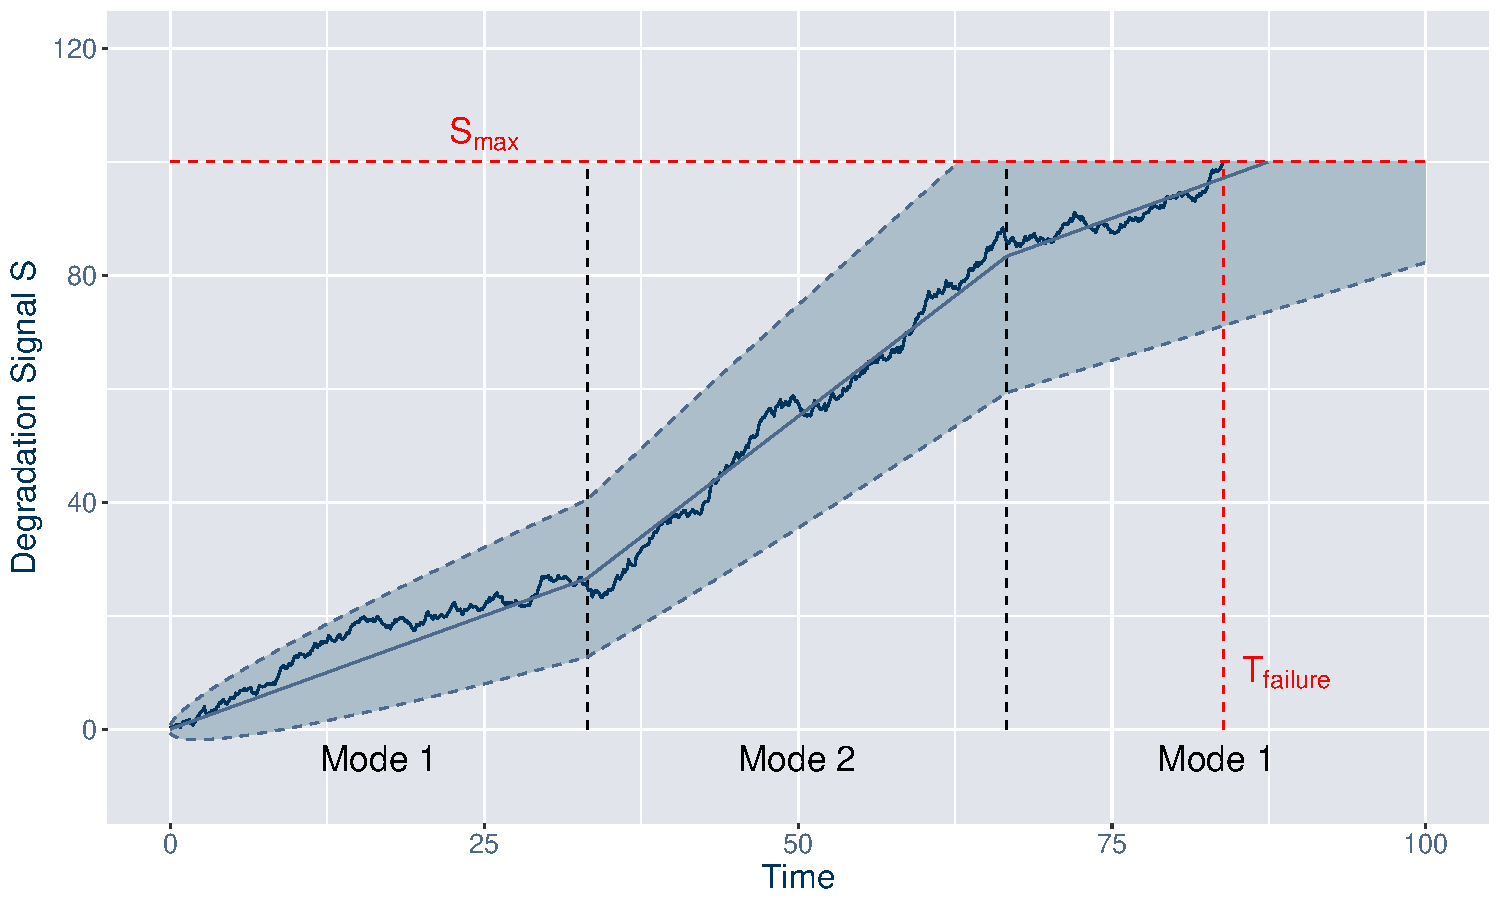
\includegraphics[scale=0.46]{example-wiener-om.pdf} \\
\end{center}
\end{frame}

\begin{frame}{How does robust optimization work?}
\begin{block}{General idea}
    \begin{itemize}
        \item Make constraints hold for all values in $\mathcal{U}$: $\sum_{j}{\tilde{a}_{ij}x_j} \leq b_i,
        \forall \tilde{a}_{ij} \in \mathcal{U}$
        \item Reformulate semi-infinite constraint:
        $\sum_{j}{a_{ij}x_j} + \text{protection}\left(\mathcal{U}\right) \leq b_i$
        \item{\color{imperialAlertText} How do we choose the right protection level?}
    \end{itemize}
\end{block}

    \begin{exampleblock}{Example: Soyster's method (worst case) [1973]}
        \vspace{-10pt}
        \begin{minipage}[t]{.4\linewidth}
            \begin{equation*}
            \begin{aligned}
            & \max_{x_1,x_2}
            && x_1 + x_2\\
            & \text{s.t.}
            && \tilde{a}_{11} x_1 + \tilde{a}_{12} x_2 \leq b_1,\\
            &
            && \forall \tilde{a}_{ij} \in \mathcal{U}\\
            \end{aligned}
            \end{equation*}
        \end{minipage}
        \hfill\vline\hfill
        \begin{minipage}[t]{.58\linewidth}
            \begin{equation*}
            \begin{aligned}
            & \max_{x_1,x_2}
            && x_1 + x_2\\
            & \text{s.t.}
            && a_{11} x_1 + a_{12} x_2  + \sum_{j}{\hat{a}_{ij}\abs{x_j}}  \leq b_1
            \end{aligned}
            \end{equation*}
        \end{minipage}
        %\vspace{10pt}
        \begin{equation*}
        \text{Given: }[a_{11}, a_{12}] = [1,2], [\hat{a}_{11}, \hat{a}_{12}] = [0.1, 0.2], [b_1] = [2]
        \end{equation*}
    \end{exampleblock}
\end{frame}

\begin{frame}{Formulation}
\begin{block}{Scheduling}
    \vspace{-20pt}
    \begin{equation*}
    \begin{aligned}
    & M_{j,t} S_{j,0} \leq S_{j,t} \leq S_{j,max} + M_{j,t} \cdot (S_{j,0} - S_{j,max})
    && \forall t, j \in J, D \in \mathcal{D}\\
    & S_{j,t} \geq S_{j,t-\Delta t} + \sum_{k}{Z_{j,k,t}D_{j,k,t}} + M_{j,t} \cdot (S_{j,0} - S_{j,max})
    && \forall t, j \in J, D \in \mathcal{D}\\
    & S_{j,t} \leq S_{j,t-\Delta t} + \sum_{k}{Z_{j,k,t}D_{j,k,t}}
    && \forall t, j \in J, D \in \mathcal{D}\\
    \end{aligned}
    \end{equation*}
    \vspace{-10pt}
\end{block}
\begin{block}{Planning}
    \vspace{-20pt}
    \begin{equation*}
    \begin{aligned}
    & S_{j,t} \leq S_{j,max}
    && \forall t, j \in J\\
    & S_{j,t} \geq S_{j,t-\Delta t} + \sum_{k}{N_{j,k,t}D_{j,k,t}} + M_{j,t} \cdot (S_{j,0} - S_{j,max})
    && \forall t, j \in J\\
    & S_{j,t} \leq S_{j,t-\Delta t} + \sum_{k}{N_{j,k,t}D_{j,k,t}}
    && \forall t, j \in J\\
    \end{aligned}
    \end{equation*}
    \vspace{-10pt}
\end{block}

\end{frame}

\begin{frame}{Adjustable robust optimization}
\begin{block}{Affine decision rule}
\begin{equation}
S_{j,t} = [S_{j,t}]_{0} + \sum_{k}\sum_{t'=0}^t{[S_{j,t}]_{k,t'}D_{j,k,t'}}.
\end{equation}
\end{block}
\end{frame}


\begin{frame}{Size of toy problem}
    \footnotesize
    \centering
    \begin{tabular}{|l|c|c|c|} \hline
         & deterministic & robust $D \neq f(t)$ & robust $D = f(t)$ \\ \hline
        \# vars & 913 & 3011 & 27719\\
        \# binaries & 338 & 338 & 338\\
        \# constraints & 1198 & 2356 & 13300\\ \hline
        time to solve [s] & 2 & 0.3-10 & 0.3-10\\
        gap [\%] & 0 & 0 & 0 \\ \hline
        scheduling periods & 30 & 30 & 30\\
        planning periods & 8 & 8 & 8\\
        \makecell[l]{task-unit-op. mode\\ combinations} & 6 & 6 & 6\\\hline
    \end{tabular}
\end{frame}

\begin{frame}{Size of realistic problem}
    \footnotesize
    \centering
    \begin{tabular}{|l|c|c|c|} \hline
        & deterministic & robust $D \neq f(t)$ & robust $D = f(t)$ \\ \hline
        \# vars & 5389 &  & 397361\\
        \# binaries & 2492 &  & 2492\\
        \# constraints & 6798 & & 180858\\ \hline
        time to solve [s] & 7883 &  & 16756\\
        gap [\%] & 3.62 &  & 31.02\\ \hline
        scheduling periods & 56 & 56 & 56\\
        planning periods & 24 & 24 & 24\\
        \makecell[l]{task-unit-op. mode\\ combinations} & 24 & 24 & 24\\ \hline
    \end{tabular}
\end{frame}

\begin{frame}{How do we choose $\mathcal{U}$?}
    \vspace{-10pt}
    \begin{block}{Choose $\mathcal{U}$ from distribution}
        \begin{minipage}[t]{.47\textwidth}
            \begin{itemize}
                \item Choose parameter $\alpha$
                \item Choose $D_{min}$ such that $P(D \leq D_{min}) = \alpha$
                \item Choose $D_{max}$ such that $P(D \geq D_{max}) = \alpha$
                \item $\mathcal{U} = \{D|D_{min} \leq D \leq D_{max}\}$
            \end{itemize}
        \end{minipage}
        \hfill\hfill
        \begin{minipage}[t]{.47\textwidth}
            \begin{center}
                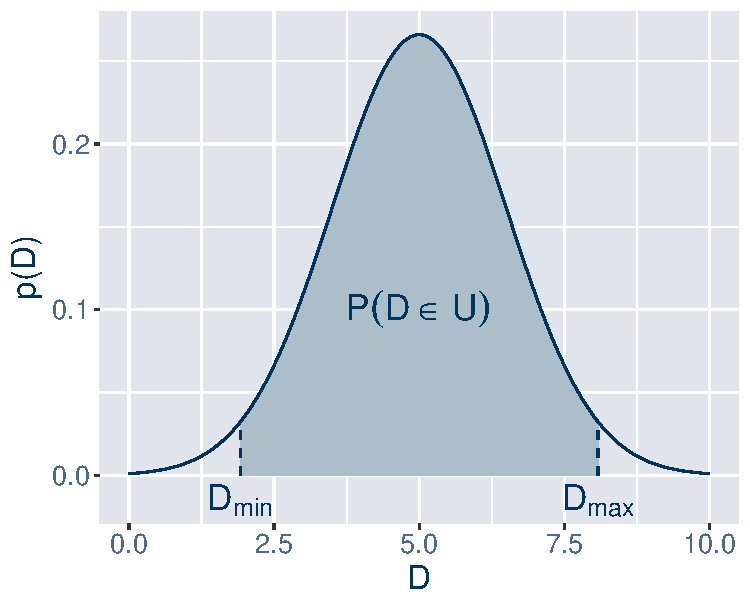
\includegraphics[scale=0.45]{uncertainty-set.pdf} \\
            \end{center}
        \end{minipage}
    \end{block}
\end{frame}

\begin{frame}{Deriving a robust counterpart}
%\begin{block}{Random variables can be replaced by uncertain parameters}
    \scriptsize
    Replace $D_{j,k}$ by an uncertain parameter $\tilde{d}_{j,k}$ bounded by a set $\mathcal{U}$:
    \vspace{-10pt}
    \begin{equation*}
    \begin{aligned}
    &
    && s_{j,t} \leq s_{j}^{max}
    &&& \forall t, j \in J\\
    &
    && s_{j,t} =
    \begin{cases}
    s_{j,t-1} + \sum_{k \in \mathcal{K}}{x_{j,k,t}\cdot \tilde{d}_{j,k}}, & \text{if } m_{j,t} = 0\\
    s_{j}^{0}, & \text{otherwise}
    \end{cases}
    &&& \forall \tilde{d}_{j,k} \in \mathcal{U}, t, j \in J\\
    \end{aligned}
    \end{equation*}
    \vspace{-5pt}
    Reformulate:
    \vspace{-5pt}
    \begin{equation*}
    \begin{aligned}
    & m_{j,t} s_{j}^{0} \leq s_{j,t} \leq s_{j}^{max} + m_{j,t} \cdot (s_{j}^{0} - s_{j,max})
    && \forall t, j \in J, \tilde{d}_{j,k} \in \mathcal{U}\\
    & s_{j,t} \geq s_{j,t-\Delta t} + \sum_{k}{x_{j,k,t}\tilde{d}_{j,k}} + m_{j,t} \cdot (s_{j}^{0} - s_{j}^{max})
    && \forall t, j \in J, \tilde{d}_{j,k} \in \mathcal{U}\\
    & s_{j,t} \leq s_{j,t-\Delta t} + \sum_{k}{x_{j,k,t}\tilde{d}_{j,k}}
    && \forall t, j \in J, \tilde{d}_{j,k} \in \mathcal{U},\\
    \end{aligned}
    \end{equation*}
Replace $s_{j,t}$ by linear decision rule $s_{j,t} = [s_{j,t}]_{0} + \sum_{k}{[s_{j,t}]_{k}\tilde{d}_{j,k}}$.
%\end{block}
\end{frame}


\begin{frame}{Results: metrics data-driven approximation}
    \begin{table}[ht]
        \label{tab:metrics-inst}
        \centering
        \begin{tabular}{llrrr}
            \hline
            instance & bound & rms\_all & rms\_max & p\_out \\
            \hline
            toy & freq & 8.00 & 1.53 & 29.40 \\
            toy & mc & 10.41 & 3.08 & 21.27 \\
            P1 & freq & 12.61 & 3.52 & 17.54 \\
            P1 & mc & 17.25 & 4.39 & 9.62 \\
            P2 & freq & 7.40 & 2.31 & 18.08 \\
            P2 & mc & 13.68 & 4.98 & 10.13 \\
            P4 & freq & 9.17 & 3.27 & 47.78 \\
            P4 & mc & 11.43 & 2.84 & 32.50 \\
            P6 & freq & 18.75 & 8.94 & 12.17 \\
            P6 & mc & 20.84 & 10.09 & 10.98 \\
            \hline
            all & freq & 11.19 & 3.91 & 24.99 \\
            all & mc & 14.72 & 5.08 & 16.90 \\
            \hline
        \end{tabular}
    \end{table}
\end{frame}

\end{document}
